% Options for packages loaded elsewhere
% Options for packages loaded elsewhere
\PassOptionsToPackage{unicode}{hyperref}
\PassOptionsToPackage{hyphens}{url}
\PassOptionsToPackage{dvipsnames,svgnames,x11names}{xcolor}
%
\documentclass[
  letterpaper,
  10pt,
  krantz2,
  titlepage,
  letterpaper]{krantz}
\usepackage{xcolor}
\usepackage{amsmath,amssymb}
\setcounter{secnumdepth}{5}
\usepackage{iftex}
\ifPDFTeX
  \usepackage[T1]{fontenc}
  \usepackage[utf8]{inputenc}
  \usepackage{textcomp} % provide euro and other symbols
\else % if luatex or xetex
  \usepackage{unicode-math} % this also loads fontspec
  \defaultfontfeatures{Scale=MatchLowercase}
  \defaultfontfeatures[\rmfamily]{Ligatures=TeX,Scale=1}
\fi
\usepackage{lmodern}
\ifPDFTeX\else
  % xetex/luatex font selection
\fi
% Use upquote if available, for straight quotes in verbatim environments
\IfFileExists{upquote.sty}{\usepackage{upquote}}{}
\IfFileExists{microtype.sty}{% use microtype if available
  \usepackage[]{microtype}
  \UseMicrotypeSet[protrusion]{basicmath} % disable protrusion for tt fonts
}{}
\makeatletter
\@ifundefined{KOMAClassName}{% if non-KOMA class
  \IfFileExists{parskip.sty}{%
    \usepackage{parskip}
  }{% else
    \setlength{\parindent}{0pt}
    \setlength{\parskip}{6pt plus 2pt minus 1pt}}
}{% if KOMA class
  \KOMAoptions{parskip=half}}
\makeatother
% Make \paragraph and \subparagraph free-standing
\makeatletter
\ifx\paragraph\undefined\else
  \let\oldparagraph\paragraph
  \renewcommand{\paragraph}{
    \@ifstar
      \xxxParagraphStar
      \xxxParagraphNoStar
  }
  \newcommand{\xxxParagraphStar}[1]{\oldparagraph*{#1}\mbox{}}
  \newcommand{\xxxParagraphNoStar}[1]{\oldparagraph{#1}\mbox{}}
\fi
\ifx\subparagraph\undefined\else
  \let\oldsubparagraph\subparagraph
  \renewcommand{\subparagraph}{
    \@ifstar
      \xxxSubParagraphStar
      \xxxSubParagraphNoStar
  }
  \newcommand{\xxxSubParagraphStar}[1]{\oldsubparagraph*{#1}\mbox{}}
  \newcommand{\xxxSubParagraphNoStar}[1]{\oldsubparagraph{#1}\mbox{}}
\fi
\makeatother

\usepackage{color}
\usepackage{fancyvrb}
\newcommand{\VerbBar}{|}
\newcommand{\VERB}{\Verb[commandchars=\\\{\}]}
\DefineVerbatimEnvironment{Highlighting}{Verbatim}{commandchars=\\\{\}}
% Add ',fontsize=\small' for more characters per line
\usepackage{framed}
\definecolor{shadecolor}{RGB}{241,243,245}
\newenvironment{Shaded}{\begin{snugshade}}{\end{snugshade}}
\newcommand{\AlertTok}[1]{\textcolor[rgb]{0.68,0.00,0.00}{#1}}
\newcommand{\AnnotationTok}[1]{\textcolor[rgb]{0.37,0.37,0.37}{#1}}
\newcommand{\AttributeTok}[1]{\textcolor[rgb]{0.40,0.45,0.13}{#1}}
\newcommand{\BaseNTok}[1]{\textcolor[rgb]{0.68,0.00,0.00}{#1}}
\newcommand{\BuiltInTok}[1]{\textcolor[rgb]{0.00,0.23,0.31}{#1}}
\newcommand{\CharTok}[1]{\textcolor[rgb]{0.13,0.47,0.30}{#1}}
\newcommand{\CommentTok}[1]{\textcolor[rgb]{0.37,0.37,0.37}{#1}}
\newcommand{\CommentVarTok}[1]{\textcolor[rgb]{0.37,0.37,0.37}{\textit{#1}}}
\newcommand{\ConstantTok}[1]{\textcolor[rgb]{0.56,0.35,0.01}{#1}}
\newcommand{\ControlFlowTok}[1]{\textcolor[rgb]{0.00,0.23,0.31}{\textbf{#1}}}
\newcommand{\DataTypeTok}[1]{\textcolor[rgb]{0.68,0.00,0.00}{#1}}
\newcommand{\DecValTok}[1]{\textcolor[rgb]{0.68,0.00,0.00}{#1}}
\newcommand{\DocumentationTok}[1]{\textcolor[rgb]{0.37,0.37,0.37}{\textit{#1}}}
\newcommand{\ErrorTok}[1]{\textcolor[rgb]{0.68,0.00,0.00}{#1}}
\newcommand{\ExtensionTok}[1]{\textcolor[rgb]{0.00,0.23,0.31}{#1}}
\newcommand{\FloatTok}[1]{\textcolor[rgb]{0.68,0.00,0.00}{#1}}
\newcommand{\FunctionTok}[1]{\textcolor[rgb]{0.28,0.35,0.67}{#1}}
\newcommand{\ImportTok}[1]{\textcolor[rgb]{0.00,0.46,0.62}{#1}}
\newcommand{\InformationTok}[1]{\textcolor[rgb]{0.37,0.37,0.37}{#1}}
\newcommand{\KeywordTok}[1]{\textcolor[rgb]{0.00,0.23,0.31}{\textbf{#1}}}
\newcommand{\NormalTok}[1]{\textcolor[rgb]{0.00,0.23,0.31}{#1}}
\newcommand{\OperatorTok}[1]{\textcolor[rgb]{0.37,0.37,0.37}{#1}}
\newcommand{\OtherTok}[1]{\textcolor[rgb]{0.00,0.23,0.31}{#1}}
\newcommand{\PreprocessorTok}[1]{\textcolor[rgb]{0.68,0.00,0.00}{#1}}
\newcommand{\RegionMarkerTok}[1]{\textcolor[rgb]{0.00,0.23,0.31}{#1}}
\newcommand{\SpecialCharTok}[1]{\textcolor[rgb]{0.37,0.37,0.37}{#1}}
\newcommand{\SpecialStringTok}[1]{\textcolor[rgb]{0.13,0.47,0.30}{#1}}
\newcommand{\StringTok}[1]{\textcolor[rgb]{0.13,0.47,0.30}{#1}}
\newcommand{\VariableTok}[1]{\textcolor[rgb]{0.07,0.07,0.07}{#1}}
\newcommand{\VerbatimStringTok}[1]{\textcolor[rgb]{0.13,0.47,0.30}{#1}}
\newcommand{\WarningTok}[1]{\textcolor[rgb]{0.37,0.37,0.37}{\textit{#1}}}

\usepackage{longtable,booktabs,array}
\usepackage{calc} % for calculating minipage widths
% Correct order of tables after \paragraph or \subparagraph
\usepackage{etoolbox}
\makeatletter
\patchcmd\longtable{\par}{\if@noskipsec\mbox{}\fi\par}{}{}
\makeatother
% Allow footnotes in longtable head/foot
\IfFileExists{footnotehyper.sty}{\usepackage{footnotehyper}}{\usepackage{footnote}}
\makesavenoteenv{longtable}
\usepackage{graphicx}
\makeatletter
\newsavebox\pandoc@box
\newcommand*\pandocbounded[1]{% scales image to fit in text height/width
  \sbox\pandoc@box{#1}%
  \Gscale@div\@tempa{\textheight}{\dimexpr\ht\pandoc@box+\dp\pandoc@box\relax}%
  \Gscale@div\@tempb{\linewidth}{\wd\pandoc@box}%
  \ifdim\@tempb\p@<\@tempa\p@\let\@tempa\@tempb\fi% select the smaller of both
  \ifdim\@tempa\p@<\p@\scalebox{\@tempa}{\usebox\pandoc@box}%
  \else\usebox{\pandoc@box}%
  \fi%
}
% Set default figure placement to htbp
\def\fps@figure{htbp}
\makeatother


% definitions for citeproc citations
\NewDocumentCommand\citeproctext{}{}
\NewDocumentCommand\citeproc{mm}{%
  \begingroup\def\citeproctext{#2}\cite{#1}\endgroup}
\makeatletter
 % allow citations to break across lines
 \let\@cite@ofmt\@firstofone
 % avoid brackets around text for \cite:
 \def\@biblabel#1{}
 \def\@cite#1#2{{#1\if@tempswa , #2\fi}}
\makeatother
\newlength{\cslhangindent}
\setlength{\cslhangindent}{1.5em}
\newlength{\csllabelwidth}
\setlength{\csllabelwidth}{3em}
\newenvironment{CSLReferences}[2] % #1 hanging-indent, #2 entry-spacing
 {\begin{list}{}{%
  \setlength{\itemindent}{0pt}
  \setlength{\leftmargin}{0pt}
  \setlength{\parsep}{0pt}
  % turn on hanging indent if param 1 is 1
  \ifodd #1
   \setlength{\leftmargin}{\cslhangindent}
   \setlength{\itemindent}{-1\cslhangindent}
  \fi
  % set entry spacing
  \setlength{\itemsep}{#2\baselineskip}}}
 {\end{list}}
\usepackage{calc}
\newcommand{\CSLBlock}[1]{\hfill\break\parbox[t]{\linewidth}{\strut\ignorespaces#1\strut}}
\newcommand{\CSLLeftMargin}[1]{\parbox[t]{\csllabelwidth}{\strut#1\strut}}
\newcommand{\CSLRightInline}[1]{\parbox[t]{\linewidth - \csllabelwidth}{\strut#1\strut}}
\newcommand{\CSLIndent}[1]{\hspace{\cslhangindent}#1}



\setlength{\emergencystretch}{3em} % prevent overfull lines

\providecommand{\tightlist}{%
  \setlength{\itemsep}{0pt}\setlength{\parskip}{0pt}}



 


%%%%%%%%%%%%%%%  Start of preamble.tex %%%%%%%%%%%%%%%%%% 
%%%%%%%%%%%%%%%  --------------------- %%%%%%%%%%%%%%%%%%
\usepackage{booktabs}
\usepackage{longtable}
\usepackage[bf,singlelinecheck=off]{caption}
\usepackage{url}

\usepackage{framed}
\usepackage{color}  % is this needed?
\definecolor{shadecolor}{RGB}{248,248,248}
\usepackage[cmyk]{xcolor} % CRC wants CMYK
% custom colors
\definecolor{darkgreen}{RGB}{1,50,32}

%%%% section headings %%%%


% https://tex.stackexchange.com/questions/750528/how-to-change-color-of-section-title-in-the-krantz-cls/750529#750529
\renewcommand\SectionHeadFont{\color{blue}\fontsize{12}{14}\sffamily\bfseries\selectfont}
\renewcommand\SubsectionHeadFont{\color{blue}\fontsize{11}{13}\sffamily\bfseries\selectfont}
\renewcommand\SubsubsectionHeadFont{\color{blue}\fontsize{10}{12}\sffamily\bfseries\selectfont}


% Define a custom color
% dark greenish-brown color, with a hexadecimal equivalent of #1A7F33
\definecolor{mygreen}{rgb}{0.1, 0.5, 0.2} 

%%%% Page headers %%%%%%
% override krantz default to use chapter/section headers
\makeatletter
\def\HeadingsChapterSection{%
  \def\chaptermark##1{%
    \markboth{%
      \thechapter. ##1}{}}%
  \def\sectionmark##1{%
    \markright{%
      \thesection: ##1}}}
\HeadingsChapterSection


% block quotes
\definecolor{quotecolor}{RGB}{0,0,100} % Example: blue
\renewenvironment{quote}
{%
  \list{}{\rightmargin=\leftmargin}%
  \item\relax\color{quotecolor}% <-- Apply the color here
  \sffamily
}
{%
  \endlist
}

%--- Cover page
% Run:
%   pdftk A=images/cover-ellipse.pdf B=index.pdf cat A1 B2-end output index-cover.pdf
%   BUT: this changes the structure of the PDF-- no bookmarks, etc.,
%   What is needed is to open index.pdf and INSERT the cover as the first page.
%   pdftk A=index.pdf B=images/cover-ellipse.pdf cat A0 B1 A2-end output index-cover.pdf
%   --> Did this manually in Adobe Acrobat Pro WORKED

% floats
\renewcommand{\textfraction}{0.05}
\renewcommand{\topfraction}{0.8}
\renewcommand{\bottomfraction}{0.8}
\renewcommand{\floatpagefraction}{0.75}

% for tinytable / modelsummary
\usepackage{tabularray}
\usepackage{float}
\usepackage{graphicx}
\usepackage{rotating}
\usepackage[normalem]{ulem}
\UseTblrLibrary{booktabs}
\UseTblrLibrary{siunitx}
% \newcommand{\tinytableTabularrayUnderline}[1]{\underline{#1}}
% \newcommand{\tinytableTabularrayStrikeout}[1]{\sout{#1}}
% \NewTableCommand{\tinytableDefineColor}[3]{\definecolor{#1}{#2}{#3}}


% krantz VF format is ugly!
%\renewenvironment{quote}{\begin{VF}}{\end{VF}}

% Make \href{} into a footnote --- does this work??
\let\oldhref\href
\providecommand{\href}[2]{#2\footnote{\url{#1}}}
  
% is this needed???
% \makeatletter
% \newenvironment{kframe}{%
%   \medskip{}
%   \setlength{\fboxsep}{.8em}
%   \def\at@end@of@kframe{}%
%   \ifinner\ifhmode%
%   \def\at@end@of@kframe{\end{minipage}}%
%   \begin{minipage}{\columnwidth}%
%   \fi\fi%
%   \def\FrameCommand##1{\hskip\@totalleftmargin \hskip-\fboxsep
%   \colorbox{shadecolor}{##1}\hskip-\fboxsep
%     % There is no \\@totalrightmargin, so:
%       \hskip-\linewidth \hskip-\@totalleftmargin \hskip\columnwidth}%
%   \MakeFramed {\advance\hsize-\width
%     \@totalleftmargin\z@ \linewidth\hsize
%     \@setminipage}}%
% {\par\unskip\endMakeFramed%
%   \at@end@of@kframe}
% \makeatother
% 
% \renewenvironment{Shaded}{\begin{kframe}}{\end{kframe}}

% Suppress underfull \hbox \vbox
\setlength{\hbadness}{1000pt}
\setlength{\vbadness}{1000pt}

% Define needed colors for xcolor
\definecolor{darkgreen}{RGB}{1,50,32}

% shut up overfull boxes

\hfuzz=5.002pt

% \tableofcontents becomes undefined. Use def from article.cls
% NO LONGER NEED THIS
% \makeatletter
% \renewcommand{\contentsname}{Contents}% For example
% \providecommand{\tableofcontents}{%
%   \section*{\contentsname}
%   \@starttoc{toc}
% }


%%%%%%%%%%%%%%%%%%%%%%%%%%%%%%%%%%%%%%%%%%%%%%%%%%%%%%%%%%%%%%%%%%%%%%%
% Index generation
% Indexentry for a word/phrase (Word inserted into the text)
%%%%%%%%%%%%%%%%%%%%%%%%%%%%%%%%%%%%%%%%%%%%%%%%%%%%%%%%%%%%%%%%%%%%%%%

% \usepackage{makeidx}
% \makeindex

\usepackage[small,firstabbrev]{authorindex}
\aimaxauthors{5}   % maximum number of authors to index

\newcommand{\IX}[1]{\index{#1}#1}
\newcommand{\ix}[1]{\index{#1}}
\newcommand{\ixmain}[1]{\index{#1|textbf}}
\newcommand{\ixon}[1]{\index{#1|(}}
\newcommand{\ixoff}[1]{\index{#1|)}}

% R functions
\newcommand{\ixfunc}[1]{%
  \index{#1@\texttt{#1()}}%
 }

% R packages:  indexed under both package name and packages!
\newcommand{\ixp}[1]{%
   \index{#1@\texttt{#1} package}%
   \index{packages!#1@\texttt{#1}}%
	}

% data sets: 
\newcommand{\ixd}[1]{%
  \index{#1}
  \index{datasets!#1}
  % \index{datasets!@\texttt{#1}}
  % \index{@\texttt{#1} dataset}
  }


\urlstyle{tt}

%%%%%%%%%%%%%%%%%
% Subject index
\usepackage{imakeidx}
\makeindex[title=Subject Index,columns=2,intoc=true,options=-s latex/book.ist]

% Author index
% Author index: now using the authorindex package
\usepackage[small,firstabbrev]{authorindex}
\aimaxauthors{5}   % maximum number of authors to index
% to generate the book.ain file, run:
% perl authorindex -d book
%    requires: BIBINPUTS, BSTINPUTS
%    setx BSTINPUTS "C:/Dropbox/localtexmf/bibtex/bst"
%    setx BIBINPUTS "C:/R/Projects/Vis-MLM-book/bib"


\usepackage{amsthm}
\makeatletter
\def\thm@space@setup{%
  \thm@preskip=8pt plus 2pt minus 4pt
  \thm@postskip=\thm@preskip
}

% Fix for modelsummary problem with \num{}
\renewcommand*{\num}[1]{#1}


\makeatother

% This doesn't work
% l.300 \includegraphics
%                       [width=\textwidth]{images/cover-ellipse.jpg}

%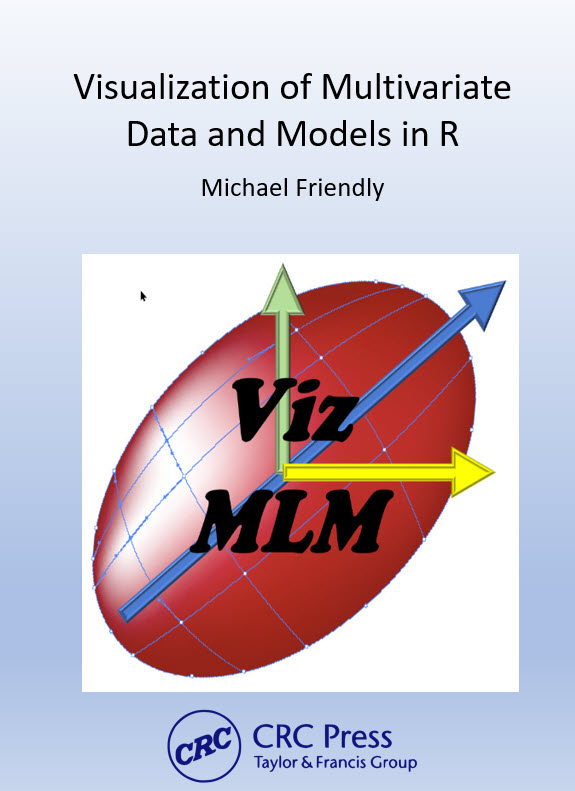
\includegraphics[width=\textwidth]{images/cover-ellipse.jpg}

\frontmatter
  
%%%%%%%%%%%%%%%  End of preamble.tex %%%%%%%%%%%%%%%%%%%%  
%%%%%%%%%%%%%%%  ------------------- %%%%%%%%%%%%%%%%%%%%
\makeatletter
\@ifpackageloaded{tcolorbox}{}{\usepackage[skins,breakable]{tcolorbox}}
\@ifpackageloaded{fontawesome5}{}{\usepackage{fontawesome5}}
\definecolor{quarto-callout-color}{HTML}{909090}
\definecolor{quarto-callout-note-color}{HTML}{0758E5}
\definecolor{quarto-callout-important-color}{HTML}{CC1914}
\definecolor{quarto-callout-warning-color}{HTML}{EB9113}
\definecolor{quarto-callout-tip-color}{HTML}{00A047}
\definecolor{quarto-callout-caution-color}{HTML}{FC5300}
\definecolor{quarto-callout-color-frame}{HTML}{acacac}
\definecolor{quarto-callout-note-color-frame}{HTML}{4582ec}
\definecolor{quarto-callout-important-color-frame}{HTML}{d9534f}
\definecolor{quarto-callout-warning-color-frame}{HTML}{f0ad4e}
\definecolor{quarto-callout-tip-color-frame}{HTML}{02b875}
\definecolor{quarto-callout-caution-color-frame}{HTML}{fd7e14}
\makeatother
\makeatletter
\@ifpackageloaded{bookmark}{}{\usepackage{bookmark}}
\makeatother
\makeatletter
\@ifpackageloaded{caption}{}{\usepackage{caption}}
\AtBeginDocument{%
\ifdefined\contentsname
  \renewcommand*\contentsname{Table of contents}
\else
  \newcommand\contentsname{Table of contents}
\fi
\ifdefined\listfigurename
  \renewcommand*\listfigurename{List of Figures}
\else
  \newcommand\listfigurename{List of Figures}
\fi
\ifdefined\listtablename
  \renewcommand*\listtablename{List of Tables}
\else
  \newcommand\listtablename{List of Tables}
\fi
\ifdefined\figurename
  \renewcommand*\figurename{Figure}
\else
  \newcommand\figurename{Figure}
\fi
\ifdefined\tablename
  \renewcommand*\tablename{Table}
\else
  \newcommand\tablename{Table}
\fi
}
\@ifpackageloaded{float}{}{\usepackage{float}}
\floatstyle{ruled}
\@ifundefined{c@chapter}{\newfloat{codelisting}{h}{lop}}{\newfloat{codelisting}{h}{lop}[chapter]}
\floatname{codelisting}{Listing}
\newcommand*\listoflistings{\listof{codelisting}{List of Listings}}
\usepackage{amsthm}
\theoremstyle{definition}
\newtheorem{example}{Example}[chapter]
\theoremstyle{definition}
\newtheorem{exercise}{Exercise}[chapter]
\theoremstyle{remark}
\AtBeginDocument{\renewcommand*{\proofname}{Proof}}
\newtheorem*{remark}{Remark}
\newtheorem*{solution}{Solution}
\newtheorem{refremark}{Remark}[chapter]
\newtheorem{refsolution}{Solution}[chapter]
\makeatother
\makeatletter
\makeatother
\makeatletter
\@ifpackageloaded{caption}{}{\usepackage{caption}}
\@ifpackageloaded{subcaption}{}{\usepackage{subcaption}}
\makeatother
\makeatletter
\@ifpackageloaded{tcolorbox}{}{\usepackage[skins,breakable]{tcolorbox}}
\makeatother
\makeatletter
\@ifundefined{shadecolor}{\definecolor{shadecolor}{rgb}{.97, .97, .97}}{}
\makeatother
\makeatletter
\@ifundefined{codebgcolor}{\definecolor{codebgcolor}{HTML}{e4f0ef}}{}
\makeatother
\makeatletter
\ifdefined\Shaded\renewenvironment{Shaded}{\begin{tcolorbox}[enhanced, sharp corners, colback={codebgcolor}, boxrule=0pt, breakable, frame hidden]}{\end{tcolorbox}}\fi
\makeatother
\usepackage{bookmark}
\IfFileExists{xurl.sty}{\usepackage{xurl}}{} % add URL line breaks if available
\urlstyle{same}
\hypersetup{
  pdftitle={Visualizing Multivariate Data and Models in R},
  pdfauthor={Michael Friendly},
  colorlinks=true,
  linkcolor={blue},
  filecolor={Maroon},
  citecolor={Blue},
  urlcolor={Blue},
  pdfcreator={LaTeX via pandoc}}


\title{Visualizing Multivariate Data and Models in R}
\usepackage{etoolbox}
\makeatletter
\providecommand{\subtitle}[1]{% add subtitle to \maketitle
  \apptocmd{\@title}{\par {\large #1 \par}}{}{}
}
\makeatother
\subtitle{A Romance in Many Dimensions}
\author{Michael Friendly}
\date{2025-10-18}
\begin{document}
\maketitle

%%%%%%%%%%%%%  START: before-body.tex ##############

\thispagestyle{empty}

{\Large Copyright page}

Cover image: \copyright Michael Friendly
Compiled: \today

First edition, published 2026 \\
by CRC Press \\
6000 Broken Sound Parkway NW, Suite 300, \\
Boca Raton FL 33487 - 2742

\copyright Michael Friendly, 2026

Rest of the stuff, ISBN, ... goes here

\cleardoublepage

% \begin{center}
% {\Large Dedication}
% 
% This book is dedicated to the many friends, colleagues, internet acquaintences and students who helped over many years in what has become this book.
% 
% Also to my life partner Martha ...
% %\includegraphics{images/dedication.pdf}
% \end{center}

\setlength{\abovedisplayskip}{-5pt}
\setlength{\abovedisplayshortskip}{-5pt}



%%%%%%%%%%%%%  END: before-body.tex ##############

\renewcommand*\contentsname{Table of contents}
{
\hypersetup{linkcolor=}
\setcounter{tocdepth}{2}
\tableofcontents
}

\bookmarksetup{startatroot}

\chapter*{Preface}\label{preface}
\addcontentsline{toc}{chapter}{Preface}

\markboth{Preface}{Preface}

This book is about graphical methods developed recently for multivariate
data, and their uses in understanding relationships when there are
several aspects to be considered together. Data visualization methods
for statistical analysis are well-developed and widely available in R
for simple linear models with a single outcome variable, as well as for
more complex models with nonlinear effects, hierarchical data with
observations grouped within larger units and so forth.

However, with applied research in the sciences, social and behavioral in
particular, it is often the case that the phenomena of interest (e.g.,
depression, job satisfaction, academic achievement, childhood ADHD
disorders, etc.) can be measured in several different ways or related
\emph{aspects}. Understanding how these different aspects are
\emph{related} can be crucial to our knowledge of the general
phenomenon.

For example, if academic achievement can be measured for adolescents by
reading, mathematics, science and history scores, how do predictors such
as parental encouragement, school environment and socioeconomic status
affect all these outcomes? In a similar way? In different ways? In such
cases, much more can be understood from a multivariate approach that
considers the correlations among the outcomes. Yet, sadly, researchers
typically examine the outcomes one by one which often only tells part of
the data story.

However, to convey the statistical and graphic methods to do these
things, I begin with some warm-up exercises in multivariate thinking,
with a grand scheme for statistics and data visualization, a parable,
and an example of multivariate discovery.

\textbf{TODO}: Include an overview of the parts and chapters somewhere
here

\section*{Features}\label{features}
\addcontentsline{toc}{section}{Features}

\markright{Features}

Some key substantive and pedagogical features of the book are:

\begin{itemize}
\item
  The writing style is purposely pedagogical (hopefully not too
  pedantic), in that it aims to teach \textbf{how to think} about
  analysis and graphics for multivariate data. That is, I try to convey
  how you can achieve \emph{understanding} of statistical concepts and
  data visualization through ways of \emph{representing those ideas} in
  diagrams and plots, and producing graphics using R functions and
  packages.
\item
  To help understand the how modern statistical and graphic methods
  became more powerful over time, the book takes a \textbf{historical
  perspective}, where it is useful to convey how the innovations we use
  today evolved.
\item
  Statistical data visualization is cast in a general framework by their
  \textbf{goal} for communicating information, either to your self or
  others (such as see the \emph{data}, visualize a \emph{model},
  diagnose \emph{problems}), rather than a categorization by
  \textbf{graphic types} like bar charts and line graphs. This is best
  informed by the principles and goals of \textbf{communication}, for
  example making graphic comparison easy and ordering factors and
  variables according to what should be seen, called \emph{effect
  ordering} for data display
  (\citeproc{ref-FriendlyKwan:03:effect}{Friendly \& Kwan, 2003}).
  \ix{effect ordering}
\item
  Data visualization is seen as a combination of
  \textbf{exposure}---plotting the raw data---and
  \textbf{summarization}--- plotting statistical summaries---to
  highlight what should be noticed. For example, data ellipses and
  confidence ellipses are widely used as simple, effective summaries of
  data and fitted model parameters. When the data is complex, the idea
  of \textbf{visual thinning} can be used to balance the tradeoff.
  \ix{visual thinning}
\item
  The book exploits the rich connections among \textbf{statistics},
  \textbf{geometry} and \textbf{data visualization}. Statistical ideas,
  particularly for multivariate data, can be more easily understood in
  terms of geometrical ones that can be seen in diagrams and data
  displays. More importantly, ideas from one domain can amplify what we
  can understand from another.
\item
  These graphical tools can be used to understand or explain a wide
  variety of statistical concepts, phenomena, and paradoxes such as
  Simpson's paradox (Section~\ref{sec-simpsons}), effects of measurement
  error (Section~\ref{sec-meas-error}), bias-variance tradeoff
  (Section~\ref{sec-bias-variance}), and so forth.
\item
  The HE (``hypothesis - error'') plot framework provides a simple way
  to understand the results of statistical tests and the relations among
  response outcomes in the multivariate linear model.
\item
  Dimension reduction techniques such as PCA and discriminant analysis
  are presented as ``multivariate juicers'', able to squeeze the
  important information in high-dimensional data into informative
  two-dimensional views. But sometimes, the most important information
  for a problem lies in the smallest dimensions, as is the case in
  outlier detection (Section~\ref{sec-multivar-normality}), collinearity
  (Section~\ref{sec-collin-biplots}) and ridge regression
  (Section~\ref{sec-ridge-low-rank}).
\end{itemize}

\section*{What I assume}\label{what-i-assume}
\addcontentsline{toc}{section}{What I assume}

\markright{What I assume}

It is assumed that the reader has at least a basic background in
\emph{applied, intermediate} statistics. This would normally include
material on simple and multiple regression as well as simple analysis of
variance (ANOVA) designs. This also means that you should be familiar
with the basic ideas of statistical inference including hypothesis tests
and confidence intervals.

There will also be some mathematics in the book where words and diagrams
are not enough. The mathematical level will be intermediate, mostly
consisting of simple algebra. No derivations, proofs, theorems here!

For multivariate methods, it will be useful to express ideas using
\textbf{matrix notation} to simplify presentation. It will be enough for
you to recognize that a single symbol \(\mathbf{y}\) can be a shorthand
for \(n\) scores on a variable like weight, and the symbol
\(\mathbf{X}\) can represent an entire data table, with, say \(n\)
observations on \(p\) variables like height, body mass index, diet
components, and so forth. Then, the notation
\(\mathbf{y} = \mathbf{X} \boldsymbol{\beta}\) represents an entire
linear model to relate weight to these other variables. I'm using this
math notation to express ideas, and all you will need is a reading-level
of understanding.

For this, the first chapter of Fox (\citeproc{ref-Fox2021}{2021}),
\emph{A Mathematical Primer for Social Statistics}, is excellent, and
the rest is well worth reading. If you want to learn something of using
matrix algebra for data analysis and statistics in R, I recommend our
package \textcolor{brown}{\texttt{\textbf{matlib}}}
(\citeproc{ref-R-matlib}{Friendly et al., 2024}) \ixp{matlib} .

\section*{R Resources}\label{r-resources}
\addcontentsline{toc}{section}{R Resources}

\markright{R Resources}

I also assume the reader to have at least a basic familiarity with
statistical analysis in R. While R fundamentals are outside the scope of
the book, I believe that this language provides a rich set of resources,
far beyond that offered by other statistical software packages, and is
well worth learning. For those not familiar with R or wish to learn new
skills, I recommend:

\begin{itemize}
\tightlist
\item
  Cotton (\citeproc{ref-Cotton-2013}{2013}), \emph{Learning R}
  (\href{http://duhi23.github.io/Analisis-de-datos/Cotton.pdf}{online})
  provides a well-rounded basic introduction to R, covering data types,
  lists and data frames, functions, packages and workflow for data
  analysis and graphics;
\item
  Matloff(\citeproc{ref-Matloff-2011}{2011}), \emph{The Art of R
  Programming}
  (\href{https://diytranscriptomics.com/Reading/files/The\%20Art\%20of\%20R\%20Programming.pdf}{online})
  is devoted to learning the programming features of R. It covers all
  the basics (data types, arrays, data frames), R functions,
  object-oriented programming, debugging, and so forth.
\item
  Wickham(\citeproc{ref-Wickham2019}{2019}), \emph{Advanced R}
  (\href{https://adv-r.hadley.nz/}{online}) is aimed at intermediate R
  programmers who want to dive deeper into R and learn how things work,
\item
  Long \& Teetor (\citeproc{ref-LongTeetor2019}{2019}), \emph{R
  Cookbook} 2\(^{nd}\) Ed (\href{https://rc2e.com/}{online}) provides
  how-to recipies for basic tasks from working with RStudio, to input
  and output, general statistics, graphics, and regression / ANOVA;
\item
  Fox \& Weisberg (\citeproc{ref-FoxWeisberg:2018}{2018a}), \emph{An R
  Companion to Applied Regression} is a fantastic resource for learning
  how to perform statistical analyses in R and visualize results with
  insightful graphics. It is the companion book to Fox's
  (\citeproc{ref-Fox:2016:ARA}{2016}), \emph{Applied Regression Analysis
  and Generalized Linear Models}, which I consider the best
  intermediate-level modern treatment of these topics. I make heavy use
  of the accompanying \textcolor{brown}{\texttt{\textbf{car}}} package
  (\citeproc{ref-R-car}{Fox \& Weisberg, 2019}) \ixp{car} which provides
  important and convenient graphical methods.
\end{itemize}

When you work with R, it may be useful to have this collection of
\href{https://friendly.github.io/6135/R/rstudio-cheat-sheets-rev3.pdf}{R
and RStudio cheatsheets} I prepared for my graduate data visualization
course.

\section*{R graphics resources}\label{r-graphics-resources}
\addcontentsline{toc}{section}{R graphics resources}

\markright{R graphics resources}

In this book, I create a large number of graphs in R, and have aimed to
present and \emph{describe} how I do them using R packages and code to
manipulate the data or numerical output from analysis function, so that
you can learn from these examples to apply these ideas to your own data.

In writing this, I've also tried to exemplify graphical principles that
underlie effective graphic communication. You might find the lecture
notes, extensive resources and R examples for my course,
\href{https://friendly.github.io/6135/}{\emph{Psychology of Data
Visualization}} useful.

In addition, there are a few books I recommend:

\begin{center}
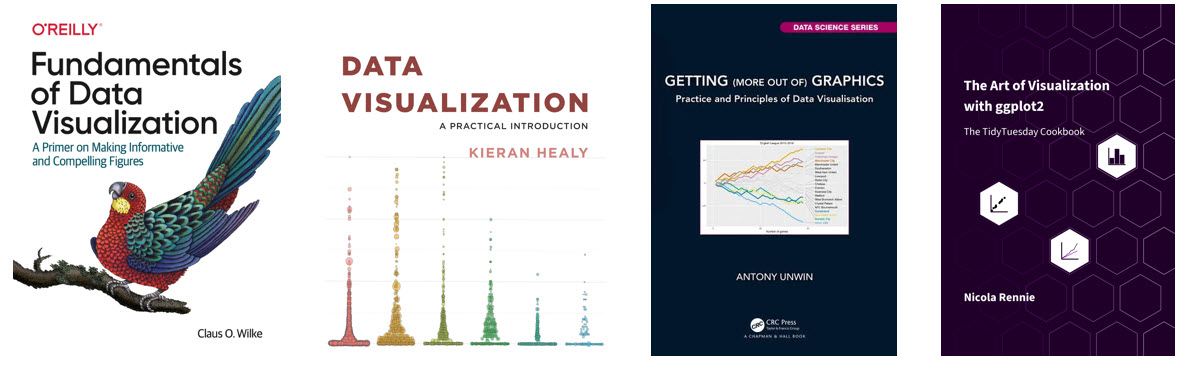
\includegraphics[width=1\linewidth,height=\textheight,keepaspectratio]{images/icons/books.jpg}
\end{center}

\begin{itemize}
\item
  Claus Wilke (\citeproc{ref-Wilke2019}{2019}), \emph{Fundamentals of
  Data Visualization} (\href{https://clauswilke.com/dataviz/}{online}) A
  well thought out presentation of important ideas of graphic
  presentation; it covers a wide range of topics, with good practical
  advice and lots of examples. How to do these in R is covered in his
  \href{https://wilkelab.org/SDS375/}{course notes}.
\item
  Keiran Healy (\citeproc{ref-Healy2019}{2019}), \emph{Data
  Visualization: A Practical Introduction}
  (\href{http://socvis.co}{online}). A highly accessible, hands-on
  primer on how to create effective graphics from data using
  \textcolor{brown}{\texttt{\textbf{ggplot2}}} \ixp{ggplot2} , with a
  focus on how to think about the information you want to show.
\item
  Antony Unwin (\citeproc{ref-Unwin2024}{2024}), \emph{Getting (more out
  of) Graphics}. This book offers a collection of 25 case studies of
  interesting datasets, exemplifying desirable features of graphs use to
  understand them and using \textcolor{brown}{\texttt{\textbf{ggplot2}}}
  \ixp{ggplot2} graphics. A second part provides useful advice on
  graphical practice, drawing on the lessons of the examples from the
  first part. The R code for all chapters is
  \href{https://github.com/antonr4/GmooGkodes}{available online}.
\item
  Nicola Rennie (\citeproc{ref-Rennie2025}{2025}), \emph{The Art of Data
  Visualization with ggplot2}
  (\href{https://nrennie.rbind.io/art-of-viz/}{online}). Rennie offers a
  kind of master class in designing effective, attractive graphics using
  \textcolor{brown}{\texttt{\textbf{ggplot2}}} \ixp{ggplot2} . The
  examples chosen stem from the
  weekly\href{https://github.com/rfordatascience/tidytuesday}{Tidy
  Tuesday} challenges that invite graphic programmers and designers to
  to work on a shared dataset to see what they can do.
\end{itemize}

\section*{R coding style used here}\label{r-coding-style-used-here}
\addcontentsline{toc}{section}{R coding style used here}

\markright{R coding style used here}

\begin{tcolorbox}[enhanced jigsaw, titlerule=0mm, bottomtitle=1mm, left=2mm, opacityback=0, bottomrule=.15mm, breakable, colframe=quarto-callout-note-color-frame, toptitle=1mm, rightrule=.15mm, opacitybacktitle=0.6, colbacktitle=quarto-callout-note-color!10!white, leftrule=.75mm, coltitle=black, arc=.35mm, title=\textcolor{quarto-callout-note-color}{\faInfo}\hspace{0.5em}{Note to reviewers}, toprule=.15mm, colback=white]

The coding style for computing and graphics used in this book are
expressed using both the traditional functional syntax, \texttt{f(g(x))}
and the newer approach using pipes (\texttt{\textbar{}\textgreater{}})
of the tidyverse. Similarly, I use both base R graphics and plots based
on the ``ggverse'' of \textcolor{brown}{\texttt{\textbf{ggplot2}}}
\ixp{ggplot2} and it's large family of add-on and extension
packages.\footnotemark{}

How and why it is this way should be explained to the reader. The
material below is a start, but needs a bit of fleshing out or editing
down.

\end{tcolorbox}

\footnotetext{The official
\href{https://exts.ggplot2.tidyverse.org/gallery/}{ggplot2 extensions
gallery website}, lists 151 registered extension packages available as
of this writing. There is also the
\href{https://ggplot2-extenders.github.io/ggplot-extension-club/}{ggplot2
extenders club}, an active group of developers organized by Gina
Reynolds and Teun van den Brand, who aim to facilitate thinking about
further growth of \texttt{ggplot} ideas and implementations.}

Like natural language and the graphic methods used in this book, R
syntax and the programming style for graphics has evolved considerably
since R was first introduced by Ross Ihaka and Robert Gentleman in 1992.
It was originally based on the S programming language
(\citeproc{ref-Becker-etal:88}{Becker et al., 1988}) and designed as a
\emph{functional} language. This means that programs are constructed by
applying and composing functions, like \texttt{log(x)}, \texttt{exp(x)},
which return a value. \ldots{}

\begin{itemize}
\tightlist
\item
  pipes
\item
  tidyverse
\item
  R graphics: \texttt{plot()} -\textgreater{} \texttt{ggplot()}
\end{itemize}

Rather than being dogmatic about using the newest, most politically
correct style,\footnote{See Norm Matloff's essay
  \href{https://matloff.github.io/TidyverseSkeptic/Skeptic.html}{Tidyverse
  Skeptic}. He argues that the tidyverse is not a good vehicle for
  teaching novice, noncoders, and that using base-R as the vehicle of
  instruction brings students to a more skilled level, in shorter time.}
in this book I have taken the view that what is most important about
programming and graphics software is that they serve as a route---as
short and direct as possible---between \textbf{having an idea} in your
head of what you want to do, and \textbf{seeing the result} on your
screen or in your report, as illustrated in Figure~\ref{fig-idea-graph}.

\begin{figure}[htb!]

\centering{

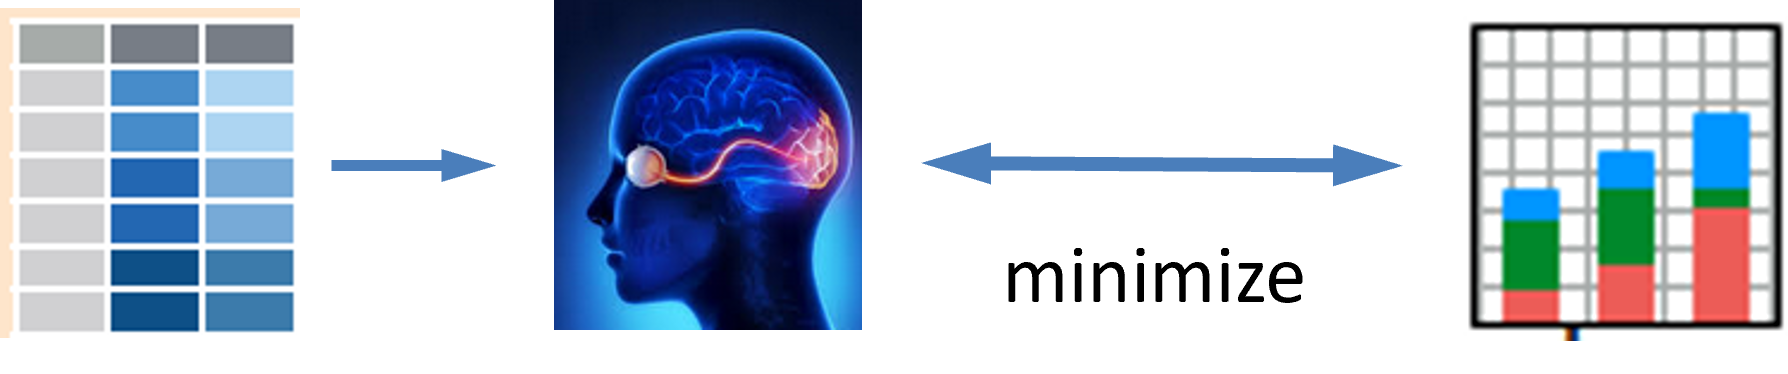
\includegraphics[width=0.8\linewidth,height=\textheight,keepaspectratio]{images/idea-graph.png}

}

\caption{\label{fig-idea-graph}The expressive power of graphics software
can be considered as minimizing the path from an idea in your head to
finished graphic.}

\end{figure}%

Consequently, for nearly every graph in this book, I used what I
considered to be the most effective style to produce an \emph{admirable
graphic}, but---perhaps more importantly--to be able to \emph{describe
how} I coded that to the reader.

For example, the \textcolor{brown}{\texttt{\textbf{car}}} package
\ixp{car} and my \textcolor{brown}{\texttt{\textbf{heplots}}}
\ixp{heplots} and related packages use base-R graphics, but I could
customize their use in examples by using the conventions of
\texttt{points()}, \texttt{lines()}, \texttt{text()} and even
\texttt{par()} when necessary. However, if I was starting this project
anew, I would now use \textcolor{brown}{\texttt{\textbf{tinyplot}}}
(\citeproc{ref-R-tinyplot}{McDermott et al., 2025}) \ixp{tinyplot} ,
which has removed many of the cringeworthy features of base-R graphics.

On the other hand, \textcolor{brown}{\texttt{\textbf{ggplot2}}} package
\ixp{ggplot2} was designed to be an \emph{elegant} language, based on
the grammar of graphics (\citeproc{ref-Wilkinson:99}{L. Wilkinson,
1999}). It allows you to \emph{think of building plots} logically and
coherently, layer by layer. Instead of memorizing specific function
calls and their arguments for every type of chart, you learn a flexible,
high-level language for describing what you \emph{want your graphic to
look like}. This promotes a more structured thinking about data
visualization, making it easier for you to iterate\footnote{You should
  think of the ``80-20'' graphics rule when you work. This says you can
  produce 80\% of your finished graphic with 20\% of your total effort.
  But the corollary is that it takes you 80\% of your time to fix the
  limitations of the remaining 20\%.}, as we always do, to create
beautiful, publication-quality graphics.

\ix{80-20 graphics rule}

This is great in theory, but as you will see here, in many code
examples, beyond the basic \texttt{geom\_*} elements, a good deal of the
effort to produce them required multiple steps to (a) get my data into a
tidy format, (b) assign proper \texttt{scale\_*}s to data variables and
(c) use \texttt{theme()} arguments to control the large and small
aspects of graphic design that contribute to the elegance and potential
beauty of finished product you see.

Consequently, this book stands on the shoulders of \emph{several} giants
in R graphics software, but the goal of reducing the gap between the
idea of a graph and the visual result can still be narrowed.

\section*{Typographic conventions used in this
book}\label{typographic-conventions-used-in-this-book}
\addcontentsline{toc}{section}{Typographic conventions used in this
book}

\markright{Typographic conventions used in this book}

The following typographic conventions are used in this book:

\begin{itemize}
\item
  \emph{italic} : indicates terms or phrases to be \emph{emphasized} or
  defined in the text; \textbf{bold} : is used for terms to be given
  \textbf{strong emphasis}, particularly for their first mention.
\item
  Package names are printed in \textbf{bold} and colored
  \textcolor{brown4}{brown}, for example
  \textcolor{brown}{\texttt{\textbf{ggplot2}}} \ixp{ggplot2} ,
  \textcolor{brown}{\texttt{\textbf{car}}} \ixp{car} and the
  \textcolor{brown}{\texttt{\textbf{matlib}}} package \ixp{matlib} .
  These uses generate citations like
  \textcolor{brown}{\texttt{\textbf{ggplot2}}}
  (\citeproc{ref-R-ggplot2}{Wickham, 2016}) \ixp{ggplot2} on their first
  use. Package references in the text are automatically indexed,
  individually and under a ``Packages'' heading.
\item
  Datasets are rendered as their name in monospaced font, like
  \texttt{Prestige} \index{Prestige@\texttt{Prestige} data}
  \index{datasets!Prestige@\texttt{Prestige}}
  \index{carData@\texttt{carData} package}
  \index{packages!carData@\texttt{carData}} or indicating the package
  from which they come, as in \texttt{carData::Prestige}
  \index{Prestige@\texttt{Prestige} data}
  \index{datasets!Prestige@\texttt{Prestige}}
  \index{carData@\texttt{carData} package}
  \index{packages!carData@\texttt{carData}}. These too are automatically
  indexed.
\item
  A monospaced \texttt{typewriter} font is used in the text to refer to
  \emph{variable} and \emph{function} names, such as \texttt{education}
  and \texttt{plot()}. This font is also for R statement elements,
  keywords and code fragments as well.
\item
  R code in program listings and output is presented in a
  \texttt{monospaced\ (typewriter)} font,
  \href{https://fonts.google.com/specimen/Fira+Mono}{\texttt{fira\ mono}}
\end{itemize}

\begin{itemize}
\tightlist
\item
  For R functions in packages, I use the notation
  \texttt{package::function()}, such as \texttt{car::Anova()}, to
  identify that the \texttt{Anova()} function is defined in the
  \textcolor{brown}{\texttt{\textbf{car}}} \ixp{car} package. This also
  means you can get help on a function by typing \texttt{?car::Anova} in
  the console, or a list of its arguments and default values from
  \texttt{args(car::Anova)}.
\end{itemize}

\section*{Acknowledgements}\label{acknowledgements}
\addcontentsline{toc}{section}{Acknowledgements}

\markright{Acknowledgements}

I am profoundly grateful to my friends and colleagues John Fox, Georges
Monette and Phil Chalmers at York University who have inspired me with
their insights into statistical thinking and visualization of
statistical ideas over many years. They also contributed greatly to the
R packages that help make the methods of this book accessible and easy
to use.

There is also a host of graduate students I have taught, supervised and
worked with over my 50+ year career. Among these, Ernest Kwan and
Matthew Sigal were important contributors to the development of data
visualization ideas and techniques reflected here. Agnieska Kopinska,
Gigi Luk and Touraj Amiri were TAs and RAs who contributed to my
teaching and research. Most recently, Udi Alter and Michael Shiuming
Truong worked as research assistants and helped me in numerous ways with
work on this book.

Writing this book using \href{https://quarto.org/}{Quarto} within the
RStudio (now \href{https://posit.co/}{Posit}) development environment
presented many technical challenges I had not encountered in previous
books (Friendly \& Meyer
(\citeproc{ref-FriendlyMeyer:2016:DDAR}{2016})). I am grateful to
Mickaël Canouil, Christophe Dervieux, Felix Benning and others in the
quarto-dev community who graciously helped me solve many issues, and
again to Michael Shiuming Truong who helped with this effort with
incisive comments, suggestions and an eagle-eye to typographic and
programming details.

The book also relies heavily on the graphic ideas and software of many R
developers, including Cory Brunson, Vincent Arel-Bundock, Di Cook, John
Fox, Duncan Murdoch, who replied to issues and feature requests on their
packages. I am also indebted to Gina Reynolds, Teun van den Brand and
other participants in the the
\href{https://ggplot2-extenders.github.io/ggplot-extension-club/}{ggplot2
extenders club} for help with \texttt{ggplot()} methods I needed for
things like labeling ``noteworthy'' observations in plots.

\mainmatter

\bookmarksetup{startatroot}

\chapter*{Author}\label{author}
\addcontentsline{toc}{chapter}{Author}

\markboth{Author}{Author}

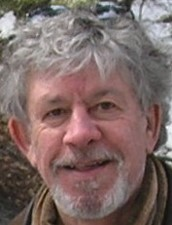
\includegraphics[width=0.3\linewidth,height=\textheight,keepaspectratio]{images/MF-gray.jpg}\hfill

\href{https://datavis.ca}{Michael Friendly} is a Fellow of the American
Statistical Association, Professor of Psychology and coordinator of the
\href{https://www.yorku.ca/research/scs/}{Statistical Consulting
Service} at York University, He is an associate editor of the
\emph{Journal of Graphical and Computational Statistics} and has served
as an editorial collaborator for many other journals. He received his
Ph.D.~in psychometrics and cognitive psychology from Princeton
University.

His current research work includes the development of graphical methods
for data visualization, where he is a principal innovator of novel
methods for relatively ``un-vizzed'' problems, including visualizing
categorical (\citeproc{ref-Friendly:00:VCD}{Friendly, 2000};
\citeproc{ref-FriendlyMeyer:2016:DDAR}{Friendly \& Meyer, 2016},) and
those for multivariate data, the subject of this book. Along with this,
he is the author and maintainer of many R packages, described on his
\href{https://github.com/friendly/friendly/blob/main/packages.md}{GitHub
R packages page}.

His passion for the deep roots of modern graphical methods led him to
become an world-known amateur historian of data visualization. In the
latter, he directs \href{http://www.datavis.ca/milestones/}{The
Milestones Project}, a comprehensive catalog and database of the
principal developments in the histories of thematic cartography,
statistical graphics and data visualization. He is a founder of an
international group, \emph{Les Chevaliers des Albums de Statistique
Graphique}, devoted to this history and is author of multiple books and
research papers on these topics. His most recent book in this area is
Friendly \& Wainer (\citeproc{ref-FriendlyWainer:2021:TOGS}{2021})
\href{https://www.hup.harvard.edu/books/9780674975231}{\emph{A History
of Data Visualization and Graphic Communication}}, Harvard University
Press.

\newpage

\pagenumbering{arabic}

\part{Orienting Ideas}

\chapter{Warm-up Exercises}\label{prelude}

\begin{tcolorbox}[enhanced jigsaw, titlerule=0mm, bottomtitle=1mm, left=2mm, opacityback=0, bottomrule=.15mm, breakable, colframe=quarto-callout-note-color-frame, toptitle=1mm, rightrule=.15mm, opacitybacktitle=0.6, colbacktitle=quarto-callout-note-color!10!white, leftrule=.75mm, coltitle=black, arc=.35mm, title=\textcolor{quarto-callout-note-color}{\faInfo}\hspace{0.5em}{Note}, toprule=.15mm, colback=white]

This will become a numbered chapter to allow cross-references, but that
entails renaming the chapter \& figures files

\end{tcolorbox}

The aim of this book is to blow your mind! Or at least to expand your
imagination and take visual thinking to higher dimensions. But, just
like kneading dough to make it more flexible before shaping and baking,
or stretching your muscles before a race or starting your car before you
drive, it is helpful to begin with some warm-up exercises, mental ones
here.

In this book, I present a number of graphical methods, some novel,
designed to help you understand multivariate data and models,
particularly when the number of variables exceeds what can easily be
shown on paper or on your screen. Visualizing these in higher dimensions
relies on ideas from geometry like projection and other analogies, and
some mathematical techniques to bridge the gap between our
three-dimensional experience and higher-dimensional realities of data
and statistical models.

To set the stage for this expedition and hopefully rouse your enthusiasm
for this endeavor, I try to pave the way for multivariate thinking with
a bit of history, a simple scheme (1-2-MANY) for statistics and data
visualization, a parable of thinking in one more dimension, and a recent
example of multivariate discovery.

\section{The Magic of Graphs}\label{the-magic-of-graphs}

\begin{quote}
\emph{There is a magic in graphs. The profile of a curve reveals in a
flash a whole situation---the life history of an epidemic, a panic, or
an era of prosperity. The curve informs the mind, awakens the
imagination, convinces.} --- Henry Hubbard, in Foreword to Brinton
(\citeproc{ref-Brinton1939}{1939}), \emph{Graphic Presentation}
\end{quote}

\begin{quote}
\emph{The graphic art depicts magnitudes to the eye. It does more. It
compels the seeing of relations. We may portray by simple graphic
methods whole masses of intricate routine, the organization of an
enterprise, or the plan of a campaign. Graphs serve as storm signals for
the manager, statesman, engineer; as potent narratives for the actuary,
statist, naturalist; and as forceful engines of research for science,
technology and industry. They display results. They disclose new facts
and laws. They reveal discoveries as the bud unfolds the flower.} ---
Henry Hubbard, in Foreword to Brinton
(\citeproc{ref-Brinton1939}{1939}), \emph{Graphic Presentation}
\end{quote}

These inspiring words were written by Henry David Hubbard, the first
Secretary of the US National Bureau of Standards (also known for
modernizing the Mendeleev's periodic table). They reflect the time in
the early 1900s when appreciation for graphical methods was widespread
and applications of graphical methods in science and popular writings
had finally become mainstream, along with textbooks (e.g., Peddle
(\citeproc{ref-Peddle:1910}{1910}); Haskell
(\citeproc{ref-Haskell:1919}{1919})) and college courses (Costelloe
(\citeproc{ref-Costelloe:1915}{1915})).

Yet, perhaps paradoxically, this period, from 1900--1950 has been called
the \emph{Modern Dark Ages} of data visualization
(\citeproc{ref-Friendly-etal:2015}{Friendly et al., 2015};
\citeproc{ref-FriendlyDenis:2001:valois}{Friendly \& Denis, 2001}).
There were few new graphical innovations and, by the mid-1930s, the
enthusiasm for visualization among statisticians had been supplanted by
the rise of quantification and formal, often statistical, models in the
social and biological sciences. Numbers---parameter estimates, and,
especially, standard errors---were \emph{precise}. Pictures were---well,
just pictures: pretty or evocative, perhaps, but incapable of stating a
``fact'' to three or more decimals. Or so it seemed to statisticians.

The re-birth of interest in data visualization among statisticians was
heralded by John Tukey (\citeproc{ref-Tukey:1962}{1962}) in ``The Future
of Data Analysis'', where he issued a call for the recognition of data
analysis as a legitimate branch of statistics distinct from mathematical
statistics. His ideas for Exploratory Data Analysis, or EDA
(\citeproc{ref-Tukey:77}{Tukey, 1977}) introduced a host of new graphic
methods (boxplots, suspended rootograms, two-way table displays, etc.),
which were soon implemented in new software systems. You probably know
the rest---an explosive growth of new ideas for high-dimensional data
and statistical models, machine learning methods, and so forth.

\subsection{Graphic discoveries,
1900--1950}\label{graphic-discoveries-19001950}

All the modern forms of data visualization---the bar and pie chart, line
graphs and the scatterplot had been invented 100 years earlier. Now, in
this period, roughly 1900--1950, graphical methods were used, perhaps
for the first time, to provide new insights, discoveries, and theories
in astronomy, physics, biology, and other sciences.

\begin{center}
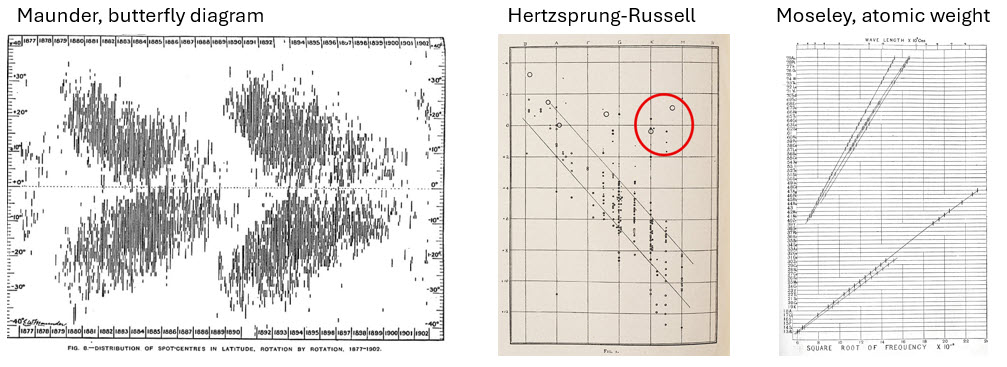
\includegraphics[width=1\linewidth,height=\textheight,keepaspectratio]{images/history/discoveries.jpg}
\end{center}

Three useful examples are:

\begin{itemize}
\item
  Edward W. Maunder (\citeproc{ref-Maunder:1904}{1904}) plotted the
  occurrence of sunspots by their latitude over time. He observed a
  consistent, repeating pattern like the wings of a butterfies, with
  sunspots drifting toward the equator in 11 year cycles. This pattern
  proved crucial for understanding the properties of the Sun's magnetic
  field.
\item
  Ejnar Hertzsprung (\citeproc{ref-Hertzsprung:1911}{1911}) and Henry
  Norris Russell (\citeproc{ref-Russell1914}{1914}) constructed plots of
  the luminosity of stars in relation to their color temperature and
  discovered an intriguing coherent pattern, but with a cluster of stars
  (``Red Giants'') detached from that main sequence. They used this to
  explain the changes as a star evolves. It provided an entirely new way
  to look at stars, and laid the groundwork for modern stellar physics
  and evolution. See Spence \& Garrison
  (\citeproc{ref-SpenceGarrison:1993}{1993}) for the full story of this
  graph.
\item
  Henry Gwyn Jeffreys Moseley (\citeproc{ref-Moseley:1913}{1913})
  discovered, largely on graphical analysis, that the concept of
  \emph{atomic number} (number of protons in an atom) rather than
  \emph{atomic weight} (protons + neutrons = weight) gave a very simple
  theory of chemical elements. His plot of serial numbers of the
  elements vs.~square root of frequencies from X-ray spectra showed a
  striking pattern of a series of straight lines. He noted gaps in the
  points and predicted the existence of several yet-undiscovered
  elements.
\end{itemize}

None of these graphs are particularly brilliant by today's standards.
They were all hand-drawn and rather crude. Yet in each case, something
previously opaque became remarkably apparent in the graphic
representation of data: a repeating pattern, some outliers departing
from the rest, or the beautiful coherence of a set of linear relations.

\section{ONE, TWO, MANY}\label{one-two-many}

To start thinking about the idea of ``dimensions'' of data and
visualization, there is an old and helpful idea I learned from John
Hartigan in my graduate days at Princeton:

\begin{quote}
\emph{In statistics and data visualization \emph{all} methods can be
classified by the number of dimensions contemplated, on a scale of
\textbf{ONE}, \textbf{TWO}, \textbf{MANY}.}
\end{quote}

By this, he meant that, at a global level, all data, statistical
summaries, and graphical displays could be classified as:

\begin{itemize}
\tightlist
\item
  \textbf{univariate}: a single variable, considered in isolation (age,
  COVID cases, pizzas ordered). Univariate numerical summaries are
  means, medians, measures of variablilty, and so forth. Univariate
  displays include dot plots, boxplots, histograms and density
  estimates.
\item
  \textbf{bivariate}: two variables, considered jointly. Numerical
  summaries include correlations, covariances and two-way tables of
  frequencies or measures of association for categorical variables.
  Bivariate displays include scatterplots and mosaic plots.
\item
  \textbf{multivariate}: three or more variables, considered jointly.
  Numerical summaries include correlation and covariance matrices,
  consisting of all pairwise values, but also derived measures from the
  analysis of these matrices (eigenvalues, eigenvectors). Graphical
  displays of multivariate data can sometimes be shown in 3D, but often
  involve multiple views of the data projected into 2D plots.
\end{itemize}

As a quasi-numerical scale, I refer to these as \textbf{1D}, \textbf{2D}
and \textbf{nD}. This admits the possibility of half-integer cases, such
as \textbf{1.5D}, where the main focus is on a single variable, but that
is classified by a simple factor (e.g., gender), or \textbf{2.5D} where
a 2D scatterplot can show other variables using color, shape or other
visual attributes. John's point in this classification was that once
you've reached three variables, all higher dimensions involve similar
summaries and data displays.

Univariate and bivariate methods and displays are well-known. This book
is about how these ideas can be extended to an \(n\)-dimensional world.
Three-dimensional data displays are now fairly easy to produce, even if
they are sometimes difficult to understand. But how can we even think
about four or more dimensions? The difficulty can be appreciated by
considering the tale of \emph{Flatland}.

\section{Flatland}\label{flatland}

\ixon{Flatland@\emph{Flatland}}

\begin{quote}
\emph{To comport oneself with perfect propriety in Polygonal society,
one ought to be a Polygon oneself.} --- Edwin A. Abbott, \emph{Flatland}
\end{quote}

In 1884, an English schoolmaster, Edwin Abbott Abbott, shook the world
of Victorian culture with a slim volume, \emph{Flatland: A Romance of
Many Dimensions} (\citeproc{ref-Abbott:1884}{Abbott, 1884}). He
described a two-dimensional world, \emph{Flatland}, inhabited entirely
by geometric figures in the plane. His purpose was satirical, to poke
fun at the social and gender class system at the time: Women were mere
line segments, while men were represented as polygons with varying
numbers of sides--- a triangle was a working man, but acute isosceles
were soldiers or criminals of very small angle; gentlemen and
professionals had more sides. Abbot published this under the pseudonym,
``A Square'', suggesting his place in the hierarchy.

\begin{quote}
\emph{True, said the Sphere; it appears to you a Plane, because you are
not accustomed to light and shade and perspective; just as in Flatland a
Hexagon would appear a Straight Line to one who has not the Art of Sight
Recognition. But in reality it is a Solid, as you shall learn by the
sense of Feeling.} --- Edwin A. Abbott, \emph{Flatland}
\end{quote}

But how did it \emph{feel} to be a member of a flatland society? How
could a point (a newborn child?) understand a line (a woman)? How does a
Triangle ``see'' a Hexagon or even a infinitely-sided Circle? Abbott
introduces the very idea of different dimensions of existence through
dreams and visions:

\begin{itemize}
\item
  A Square dreams of visiting a one-dimensional \emph{Lineland} where
  men appear as lines, and women are merely ``illustrious points'', but
  the inhabitants can only see the Square as lines.
\item
  In a vision, the Square is visited by a Sphere, to illustrate what a
  2D Flatlander could understand from a 3D sphere
  (Figure~\ref{fig-flatland-spheres}) that passes through the plane he
  inhabits. It is a large circle when seen at the moment of its'
  greatest extent. As the Spehere rises, it becomes progressively
  smaller, until it becomes a point, and then vanishes.
\end{itemize}

\begin{figure}[htb!]

\centering{

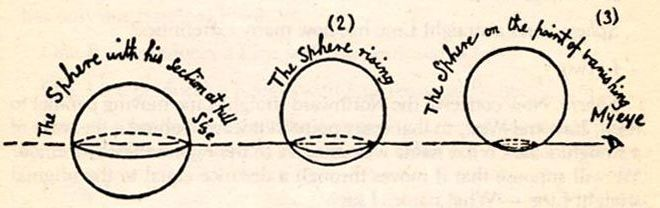
\includegraphics[width=0.9\linewidth,height=\textheight,keepaspectratio]{images/flatland-spheres.jpg}

}

\caption{\label{fig-flatland-spheres}A 2D Flatlander seeing a sphere as
it passes through Flatland. The line, labeled `My Eye' indicates what
the Flatlander would see. \emph{Source}: Abbott
(\citeproc{ref-Abbott:1884}{1884})}

\end{figure}%

Abbott goes on to state what could be considered as a demonstration (or
proof) by induction of the difficulties of seeing in 1, 2, 3 dimensions,
and how the idea motion over time (one more dimension) could allow
citizens of any 1D, 2D, 3D world to contemplate one more dimension.

\begin{quote}
\emph{In One Dimensions, did not a moving Point produce a Line with two
terminal points? In two Dimensions, did not a moving Line produce a
Square with four terminal points? In Three Dimensions, did not a moving
Square produce---did not the eyes of mine behold it---that blessed
being, a Cube, with eight terminal points? And in Four Dimensions, shall
not a moving Cube---alas, for Analogy, and alas for the Progress of
Truth if it be not so---shall not, I say the motion of a divine Cube
result in a still more divine organization with sixteen terminal
points?} --- Edwin A. Abbott
\end{quote}

For Abbot, the way for a citizen of any world to imagine one more
dimension was to consider how a higher-dimensional object would change
over time.\footnote{In his famous TV series, \emph{Cosmos}, Carl Sagan
  provides \href{https://youtu.be/UnURElCzGc0}{an intriguing video
  presentation} Flatland and the 4th dimension. However, as far back as
  1754 (\citeproc{ref-Cajori:1926}{Cajori, 1926}), the idea of adding a
  fourth dimension appears in Jean le Rond d'Alembert's ``Dimensions'',
  and one realization of a four-dimensional object is a
  \emph{tesseract}, shown in Figure~\ref{fig-1D-4D}.} A line moved over
time could produce a rectangle as shown in Figure~\ref{fig-1D-4D}; that
rectangle moving in another direction over time would produce a 3D
figure, and so forth.

\begin{figure}[htb!]

\centering{

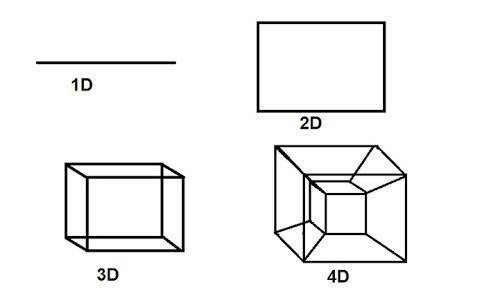
\includegraphics[width=0.9\linewidth,height=\textheight,keepaspectratio]{images/1D-4D.png}

}

\caption{\label{fig-1D-4D}Geometrical objects in 1 to 4 dimensions. One
more dimension can be thought of as the trace of movement over time.}

\end{figure}%

But wait! Where does that 4D thing (a \emph{tesseract}) come from? To
really see a tesseract it helps to view it in an animation over time
(Figure~\ref{fig-tesseract}). But like the Square, contemplating 3D from
a 2D world, it takes some imagination.

\begin{figure}[htb!]

\centering{

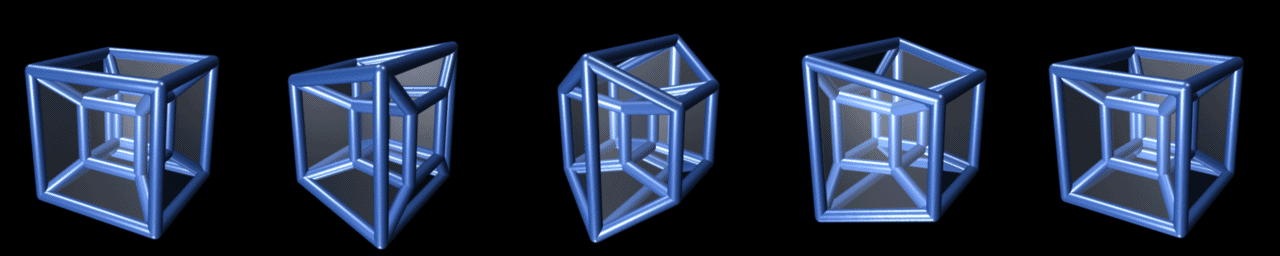
\includegraphics[width=1\linewidth,height=\textheight,keepaspectratio]{images/tesseract-frames.png}

}

\caption{\label{fig-tesseract}Five frames from an animation of a
tesseract, a cube changing through a 4th dimension over time
\emph{Source}: ediacura,
\href{https://www.youtube.com/watch?v=5xN4DxdiFrs}{YouTube}.}

\end{figure}%

Yet the deep mathematics of more than three dimensions only emerged in
the 19th century. In Newtonian mechanics, space and time were always
considered independent of each other. Our familiar three-dimensional
space, of length, width, and height had formed the backbone of Euclidean
geometry for millenea.

However, the idea that space and time are indeed interwoven was first
proposed by German mathematician Hermann Minkowski (1864--1909) in a
1908 lecture titled ``Space and Time''.\footnote{See the translation by
  Lewertoff and Petkov, ``Space and Time Minkowski's Papers on
  Relativity'', https://bit.ly/45NvgZR} This was a powerful idea. It
bore fruit when Albert Einstein revolutionized the Newtonian conceptions
of gravity in 1915 when he presented a theory of general relativity
which was based primarily on the fact that mass and energy warp the
fabric of four-dimensional spacetime.

The parable of \emph{Flatland} can provide inspiration for statistical
thinking and data visualization. Once we go beyond bivariate statistics
and 2D plots, we are in a multivariate world of possibly MANY
dimensions. It takes only some imagination and suitable methods to get
there.

Like Abbott's \emph{Flatland}, this book is a romance, in many
dimensions, of what we can learn from modern methods of data
visualization.

\ixoff{Flatland@\emph{Flatland}}

\section{EUREKA!}\label{eureka}

Even modest sized multivariate data can have secrets that can be
revealed in the right view. As an example, David Coleman at RCA
Laboratories in Princeton, N.J. generated a dataset of five (fictitious)
measurements of grains of pollen for the 1986 Data Exposition at the
Joint statistical Meetings, now available as \texttt{HistData::Pollen}
\index{Pollen@\texttt{Pollen} data}
\index{datasets!Pollen@\texttt{Pollen}}
\index{HistData@\texttt{HistData} package}
\index{packages!HistData@\texttt{HistData}}.

The first three variables are the lengths of geometric features 3848
observed sampled pollen grains -- in the x, y, and z dimensions: a
\texttt{ridge} along x, a \texttt{nub} in the y direction, and a
\texttt{crack} along the z dimension. The fourth variable is pollen
grain \texttt{weight}, and the fifth is \texttt{density}. The challenge
was to ``find something interesting'' in this dataset. \ixp{animation}

This problem is a case of searching for an unspecified needle in a five
dimensional haystack. Those who solved the puzzle were able to find an
orientation of this 5-dimensional dataset, such that zooming in revealed
a magic word, \textbf{``EUREKA''} spelled in points, as in the following
figure which shows four successive magnifications of the data
(clockwise, from the upper left).

\begin{figure}[htb!]

\begin{minipage}{0.50\linewidth}
\pandocbounded{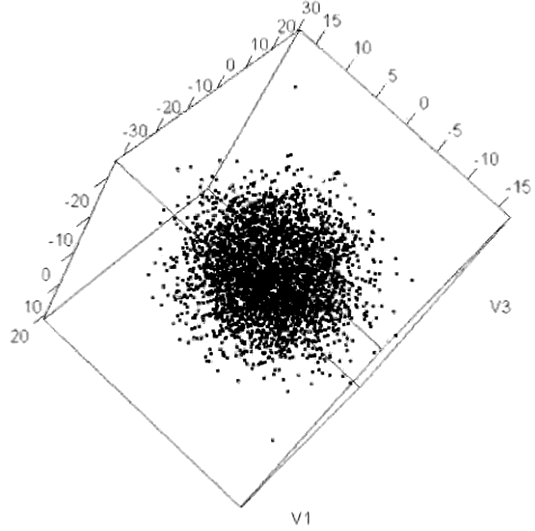
\includegraphics[keepaspectratio]{images/pollen-eureka1.png}}\end{minipage}%
%
\begin{minipage}{0.50\linewidth}
\pandocbounded{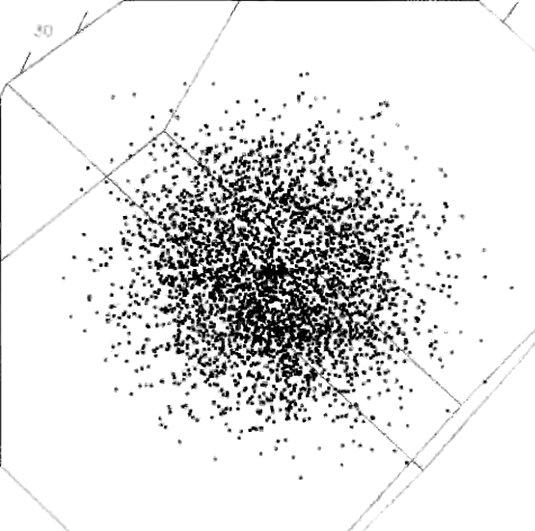
\includegraphics[keepaspectratio]{images/pollen-eureka2.png}}\end{minipage}%
\newline
\begin{minipage}{0.50\linewidth}
\pandocbounded{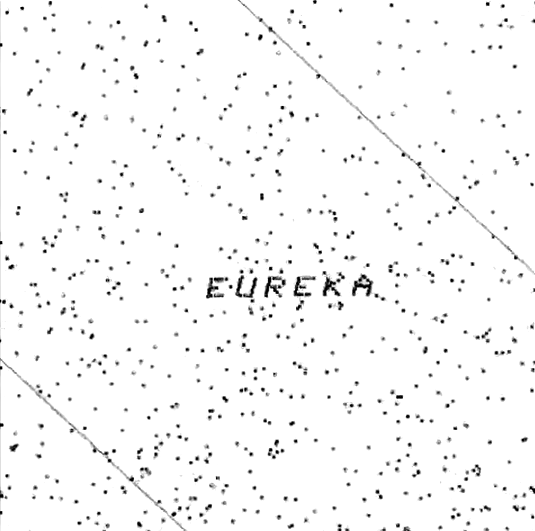
\includegraphics[keepaspectratio]{images/pollen-eureka4.png}}\end{minipage}%
%
\begin{minipage}{0.50\linewidth}
\pandocbounded{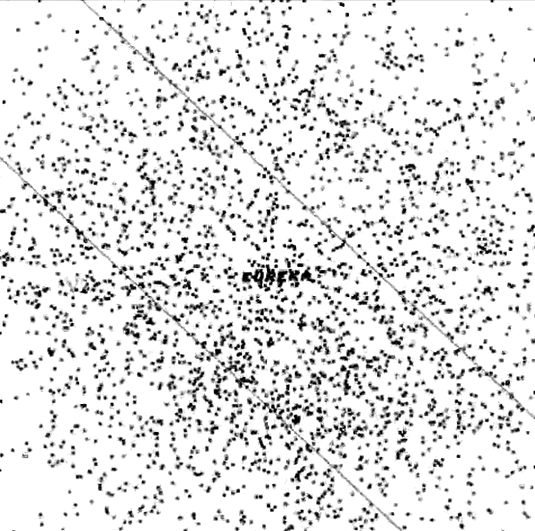
\includegraphics[keepaspectratio]{images/pollen-eureka3.png}}\end{minipage}%

\caption{\label{fig-pollen-eureka}Four views of the \texttt{pollen}
data, zooming in, clockwise from the upper left to discover the word
``EUREKA''.}

\end{figure}%

The path to finding the hidden word can be seen better in a 3D
animation. The online version of the book uses the
\textcolor{brown}{\texttt{\textbf{rgl}}} package
(\citeproc{ref-R-rgl}{Murdoch \& Adler, 2025}) \ixp{rgl} to create a 3D
scatterplot of the first three variables. Then the
\textcolor{brown}{\texttt{\textbf{animation}}} package
(\citeproc{ref-R-animation}{Xie, 2021}) \ixp{animation} is used to
record a sequence of images, adjusting the \texttt{rgl::par3d(zoom)}
value.

The vague idea of finding ``something interesting'' in high-D data was
first posed by John and Paul Tukey (\citeproc{ref-TukeyTukey:85}{1985})
as an exploratory visualization method they called \textbf{scagnostics},
short for ``scatterplot diagnostics''. L. Wilkinson et al.
(\citeproc{ref-Wilkinson-etal:2005}{2005}) made this idea concrete by
defining measures of features such as ``clumpy'', ``striated'',
``convex'', ``skinny'', and so forth. These methods are implemented in
the \textcolor{brown}{\texttt{\textbf{scagnostics}}} \ixp{scagnostics}
and \textcolor{brown}{\texttt{\textbf{cassowaryr}}} \ixp{cassowaryr}
packages.

Another idea is to search through high-D data space for views or
projections with interesting features, initially called
\textbf{projection pursuit} (\citeproc{ref-Friedman:87}{J. H. Friedman,
1987}; \citeproc{ref-FriedmanTukey:74}{J. H. Friedman \& Tukey, 1974}).
Some modern methods for this are illustrated in
Section~\ref{sec-animated-tours}.

\section{Multivariate scientific discoveries}\label{sec-discoveries}

Lest the EUREKA example seem contrived (which it admittedly is), truly
\emph{multivariate} visualization has played an important role in quite
a few scientific discoveries. Among these, Francis Galton's
(\citeproc{ref-Galton:1863}{1863}) discovery of the anti-cyclonic
pattern of wind direction in relation to barometric pressure from many
weather measures recorded systematically across all weather stations,
lighthouses and observatories in Europe in December 1861 stands out as
the best example of a scientific discovery achieved almost entirely
through graphical means---- something that was totally unexpected, and
purely the product of his use of remarkably novel high-dimensional
graphs (\citeproc{ref-FriendlyWainer:2021:TOGS}{Friendly \& Wainer,
2021, pp. 170--173}).

A more recent example is the discovery of two general classes in the
development of Type 2 diabetes by Reaven \& Miller
(\citeproc{ref-ReavenMiller:79}{1979}), using PRIM-9
(\citeproc{ref-Fishkeller-etal:1974b}{Fishkeller et al., 1974}), the
first computer system for high-dimensional visualization\footnote{PRIM-9
  is an acronym for \textbf{P}icturing, \textbf{R}otation,
  \textbf{I}solation and \textbf{M}asking in up to \textbf{9}
  dimensions. These operations are fundamental to interactive and
  dynamic data visualization.}. In an earlier study Reaven \& Miller
(\citeproc{ref-ReavenMiller:68}{1968}) examined the relation between
blood glucose levels and the production of insulin in normal subjects
and in patients with varying degrees of hyperglycemia (elevated blood
sugar level). They found a peculiar `'horse shoe'\,' shape in this
relation (shown in Figure~\ref{fig-diabetes1}), about which they could
only speculate: perhaps individuals with the best glucose tolerance also
had the lowest levels of insulin as a response to an oral dose of
glucose; perhaps those with low glucose response could secrete higher
levels of insulin; perhaps those who were low on both glucose and
insulin responses followed some other mechanism. In 2D plots, this was a
mystery. \ix{PRIM-9}

\begin{Shaded}
\begin{Highlighting}[]
\FunctionTok{data}\NormalTok{(Diabetes, }\AttributeTok{package=}\StringTok{"heplots"}\NormalTok{)}
\FunctionTok{plot}\NormalTok{(instest }\SpecialCharTok{\textasciitilde{}}\NormalTok{ glutest, }\AttributeTok{data=}\NormalTok{Diabetes, }
     \AttributeTok{pch=}\DecValTok{16}\NormalTok{,}
     \AttributeTok{cex.lab=}\FloatTok{1.25}\NormalTok{,}
     \AttributeTok{xlab=}\StringTok{"Glucose response"}\NormalTok{,}
     \AttributeTok{ylab=}\StringTok{"Insulin response"}\NormalTok{)}
\end{Highlighting}
\end{Shaded}

\begin{figure}[htb!]

\centering{

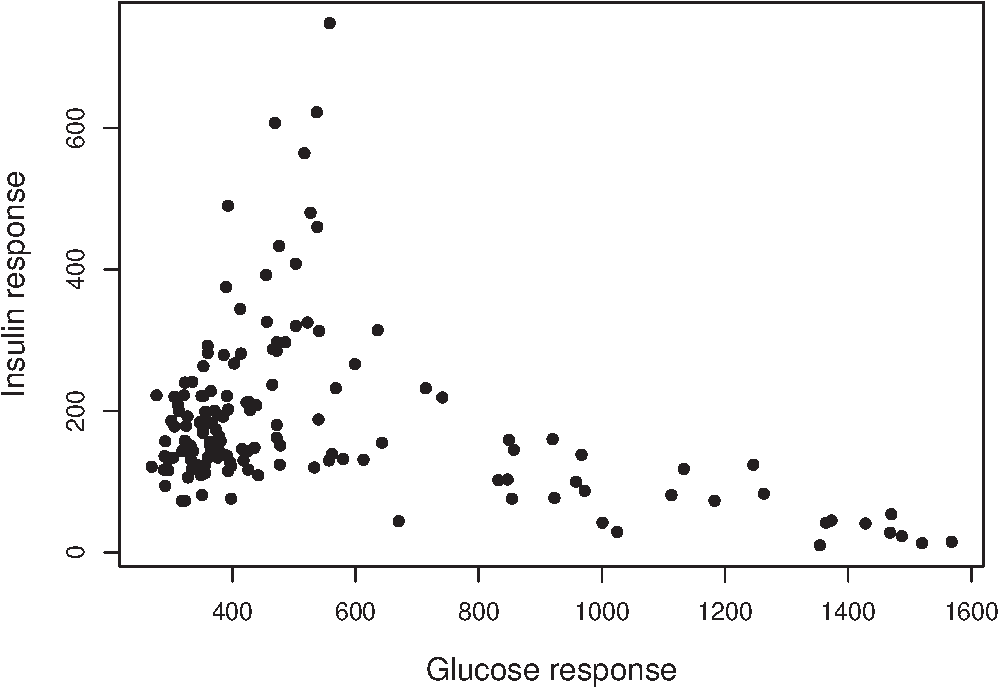
\includegraphics[width=0.7\linewidth,height=\textheight,keepaspectratio]{figs/ch01/fig-diabetes1-1.pdf}

}

\caption{\label{fig-diabetes1}Reproduction of a graph similar to that
from Reaven \& Miller (\citeproc{ref-ReavenMiller:68}{1968}) on the
relationship between glucose and insulin response to being given an oral
dose of glucose.}

\end{figure}%

An answer to their questions came ten years later, when they were able
to visualize similar but new data in 3D using the PRIM-9 system. In a
carefully controlled study, they also measured `'steady state plasma
glucose'\,' (SSPG), a measure of the efficiency of insulin use in the
body, where large values mean insulin resistance, as well as other
variables. PRIM-9 allowed them to explore various sets of three
variables, and, more importantly, to rotate a given plot in three
dimensions to search for interesting features. One plot that stood out
concerned the relation between plasma glucose response, plasma insulin
response and SSPG response, shown in Figure~\ref{fig-ReavenMiller-3d}.

\begin{figure}[htb!]

\centering{

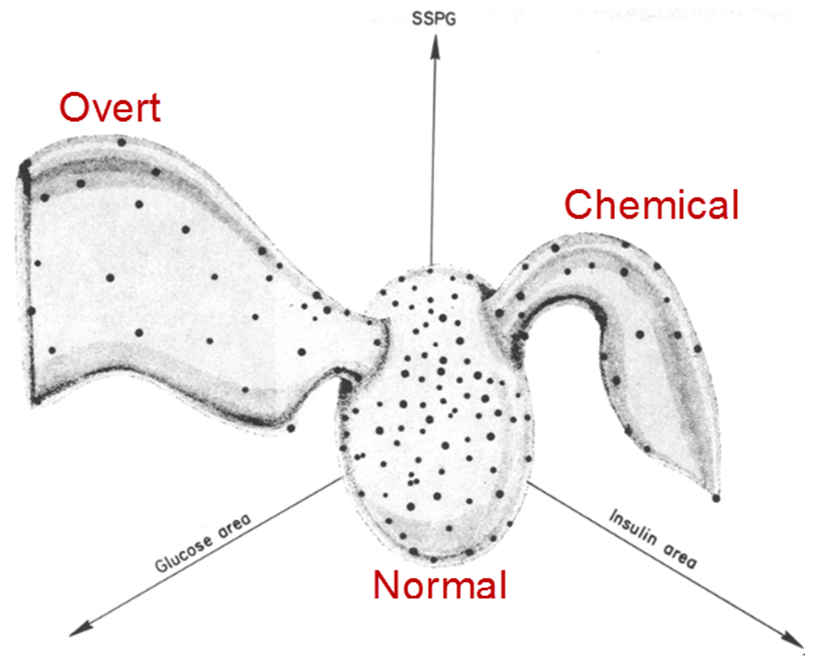
\includegraphics[width=0.7\linewidth,height=\textheight,keepaspectratio]{images/ReavenMiller-3d-annotated.png}

}

\caption{\label{fig-ReavenMiller-3d}Artist's rendition of data from
Reaven \& Miller (\citeproc{ref-ReavenMiller:79}{1979}) as seen in three
dimensions using the PRIM-9 system. Labels for the clusters have been
added, identifying the three groups of patients. \emph{Source}: Reaven
\& Miller (\citeproc{ref-ReavenMiller:79}{1979}).}

\end{figure}%

From this graphical insight, they were able to classify the participants
into three groups, based on clinical levels of glucose and insulin. The
people in the wing on the left in Figure~\ref{fig-ReavenMiller-3d} were
considered to have overt diabetes, the most advanced form, characterized
by elevated fasting blood glucose concentration and classical diabetic
symptoms. Those in the right wing were classified as latent or chemical
diabetics, with no symptoms of diabetes but demonstrable abnormality of
oral or intravenous glucose tolerance. Those in the central blob were
classified as normal.

Previous thinking was that Type 2 diabetes (when the body cannot make
\emph{enough} insulin, as opposed to Type I, an autoimmune condition
where the pancreatic cells have been destroyed) progressed from the
chemical stage to an overt one in a smooth transition. However, it was
clear from Figure~\ref{fig-ReavenMiller-3d} that the only ``path'' from
one to the other lead through the cluster of normal patients near the
origin, so that explanation must be wrong. Instead, this suggested that
the chemical and overt diabetics were distinct classes. Indeed,
longitudinal studies showed that patients classified as chemical
diabetics rarely developed the overt form. Our understanding of the
etiology of Type 2 diabetes was altered dramatically by the power of
high-D interactive graphics.

\chapter{Introduction}\label{sec-introduction}

A major goal of this book is to introduce you to multivariate thinking
in research design and data analysis. This is accomplished with a
collection of powerful graphical methods designed to make it easier to
understand and communicate results when there are multiple response
variables to be considered together. However, these methods are somewhat
more complex than the standard univariate ones, so it is worth
considering these questions: Why should you to go to this trouble?
What's in it for me?

\section{Why use a multivariate
design?}\label{why-use-a-multivariate-design}

The first important point is that \emph{reality} in many research
domains is inherently multivariate, particularly in the social and
behavioral sciences. Theoretical constructs such as ``depression'',
``academic achievement'', ``self-concept'', ``happiness'' or
``perfectionism'' can often be measured by different scales, or have
been identified to have more than one aspect or context worthy of study.

\textbf{Conceptual advantages}

Analyzing these together from a multivariate approach can reveal
relationships completely missed or ignored by simpler univariate
analyses. Theory is strengthened and becomes more nuanced from a
multivariate perspective.

You can understand each of those terms, but actually all of these
constructs are inherently multidimensional. The idea of
``self-concept'', for instance is comprised of all the beliefs that an
individual has about him/herself. These include physical, social,
intellectual, family, emotional, and professional/academic domains,
which reflect how individuals perceive their bodies, roles in society,
abilities, as well as their familial connections, and competencies in
work and school.

Even something simpler, like academic achievements of adolescents, aged
10--16 is comprised of measures of their knowledge and performance in
the domains of reading, mathematics, science, history, etc. Say we want
to assess the influence of predictors such as parent encouragement,
their socioeconomic status and school environmental variables on these
outcomes. In a comprehensive study, the following questions are of
interest:

\begin{itemize}
\item
  Do predictors (parental encouragement, \ldots) affect \emph{all} of
  these outcomes? Or do some of these have weak or null effects?
\item
  Do they affect them in the \emph{same} or \emph{different} ways? That
  is, do their effects tend to go in the same directions?
\item
  How many different \emph{aspects} of academic achievement can be
  distinguished in the predictors? Equivalently, is academic achievement
  \emph{unidimensional} or \emph{multidimensional} in relation to the
  predictors?
\end{itemize}

Similarly, if psychiatric patients in various diagnostic categories are
measured on a battery of tests related to social skills and cognitive
functioning, we might want to know:

\begin{itemize}
\item
  Which measures best discriminate among the diagnostic groups?
\item
  Which measures are most predictive of positive outcomes?
\item
  Further, how are the \emph{relationships} between the outcomes
  affected by the predictors?
\end{itemize}

Such questions obviously concern more than just the separate univariate
relations of each response to the predictors. Equally, perhaps more
importantly, are questions of how the response variables are predicted
\emph{jointly} considering their correlations that a multivariate
approach can reveal.

\begin{tcolorbox}[enhanced jigsaw, titlerule=0mm, bottomtitle=1mm, left=2mm, opacityback=0, bottomrule=.15mm, breakable, colframe=quarto-callout-note-color-frame, toptitle=1mm, rightrule=.15mm, opacitybacktitle=0.6, colbacktitle=quarto-callout-note-color!10!white, leftrule=.75mm, coltitle=black, arc=.35mm, title=\textcolor{quarto-callout-note-color}{\faInfo}\hspace{0.5em}{What about SEM?}, toprule=.15mm, colback=white]

Structural equation modeling (SEM) offers another route to explore and
analyze the relationships among multiple predictors and multiple
responses. They have the advantage of being able to test potentially
complex systems of linear equations in very flexible ways. However,
these methods are often far removed from data analysis \emph{per se}
because they typically \emph{start} with data summaries such as means
and covariance matrices. The raw data is nicely bundled up in these
summaries, but consequently there is little room to learn from features
such as non-linear relations, interesting clusters, or anomalous
observations that might threaten the validity of a proposed model. But
see Prokofieva et al. (\citeproc{ref-Prokofieva2023}{2023}) for an
approach (ESEM) using R that combines exploratory analysis with standard
SEM, or Brandmaier et al. (\citeproc{ref-Brandmaier2014}{2014}) for an
approach combining SEM and decision trees to allow data-driven
refinement of models.

Moreover, except for path diagrams, they usually offer little in the way
of visualization methods to aid in understanding and communicating the
results. The graphical methods we describe here can also be useful in a
SEM context. For example, multivariate multiple regression models
(Section~\ref{sec-MRA-to-MMRA}) and canonical correlation
(Section~\ref{sec-cancor}) can be used to explore relationships among
the observed variables used in a SEM, but in a data-centric way.
\index{Structural equation model}

\end{tcolorbox}

\textbf{Statistical advantages}

A second important point is that a multivariate modeling approach can
offer statistical advantages:

\begin{itemize}
\tightlist
\item
  They can have increased statistical power to detect a significant
  effect, because multivariate tests pool the strength of effects across
  a collection of positively related response variables.
\item
  This easily avoids inflated Type I error rates (false positives) from
  multiple separate tests on each of the outcomes.
\item
  We gain deeper insights into how outcome variables vary together.
\item
  With more than a few outcome variables \emph{dimension reduction}
  methods offer views of the data and model in 2D plots that capture
  their essence.
\end{itemize}

\subsection{Multivariate vs.~multivariable
methods}\label{multivariate-vs.-multivariable-methods}

\begin{quote}
\emph{multivariate \(\ne\) multivariable}
\end{quote}

``Multi-'' terminology is important. In this era of multivitamins,
multitools, multifactor authentication and even the multiverse, it is
well to understand the distinction between \emph{multivariate} and
\emph{multivariable} methods as these terms are generally used and as I
use them here in relation to statistical methods and data visualization.
The distinction is simple:

\begin{itemize}
\item
  \textbf{Multivariable methods} have a single dependent variable and
  more than one independent variables or covariates, such as in multiple
  regression. Multiple regression is the prime example.
\item
  \textbf{Multivariate methods} for linear models, such as multivariate
  multiple regression or multivariate analysis of variance, have more
  than one dependent, response or outcome variable. Canonical
  correlation analysis considers the relation between two sets of
  variables, but treats them symmetrically. Other multivariate methods
  such as principal components analysis or factor analysis don't
  distinguish between independent and dependent, but treat all variables
  on an equal footing in a single set.
\end{itemize}

\subsection{Ubiquity of multivariate research
designs}\label{ubiquity-of-multivariate-research-designs}

Multivariate response designs are increasingly common in applied
behavioral and social science research, and are utilized to analyze a
wide range of phenomena. For instance, as an introductory exercise,
graduate students enrolled in a multivariate data analysis
course\footnote{The web pages for this course can be found at
  \href{http://friendly.apps01.yorku.ca/psy6140/}{Psychology 6140:
  Multivariate Data Analysis}. I last taught this in 2016--2017.} in the
Psychology Department at York University between 1990 and 2015 were
asked to scan one or more journals in their area and to find at least
one paper that utilized some form of multivariate analysis.

With an average of 15--20 students per year and over approximately 20
years, this yielded a bibliographic database containing 405 exemplars
(\citeproc{ref-py614bib}{Friendly \& 6140 Members, 2012}). These used a
variety of multivariate and supplementary univariate methods, ranging
from MANOVA to path analysis, from canonical correlation to
multidimensional scaling, which were categorized by statistical method
using keyword terms.

Overall, MANOVA, factor analysis, multiple regression, correlation, and
principal components analysis were utilized the most frequently. See
Figure~\ref{fig-heatmap} for a summary of these results, using a heatmap
tabular display of frequencies by time. An overall categorization
pertaining to the type of multivariate model used (CDA = Categorical
data analysis, FA = Factor analysis, GDA = Geometric data analysis, and
LM = Linear models) is shown in the right margin. This is clearly not a
representative sample of the literature, but it does illustrate an
increase of articles deemed noteworthy over time.

\begin{figure}[htb!]

\centering{

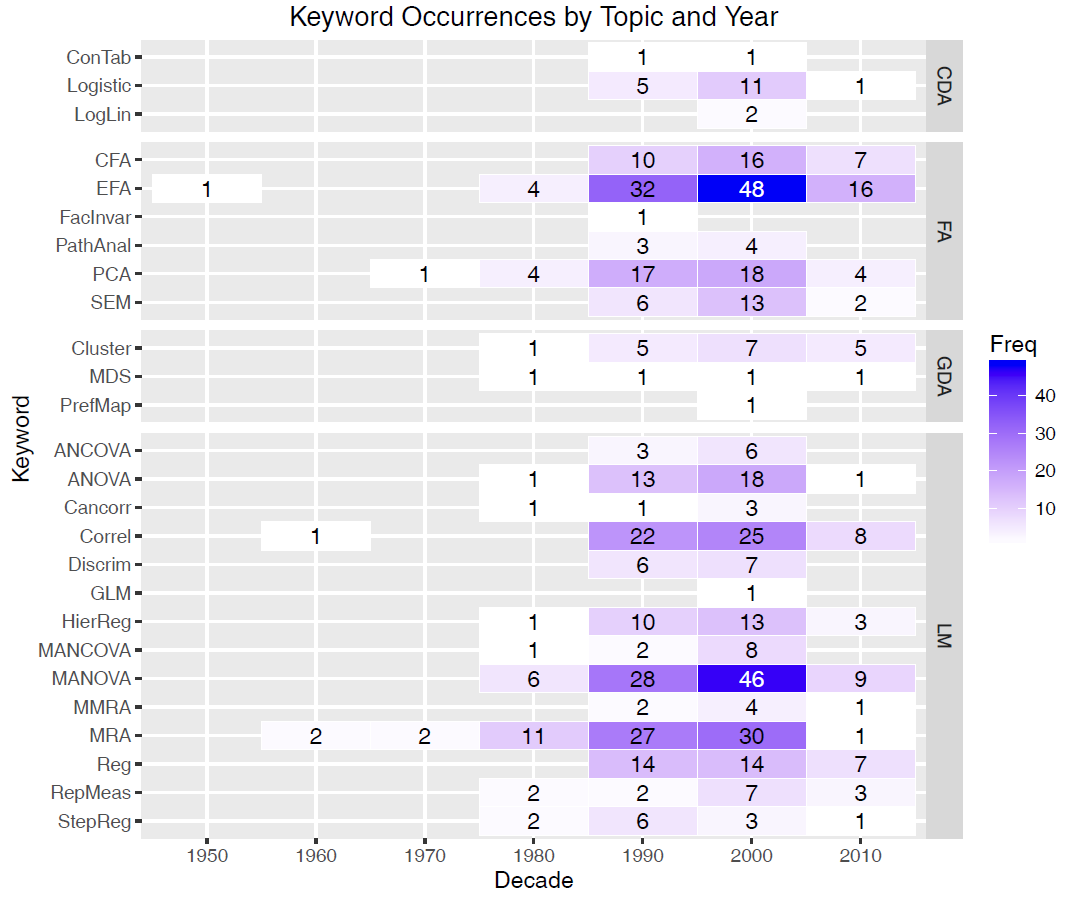
\includegraphics[width=0.7\linewidth,height=\textheight,keepaspectratio]{images/heatmap.png}

}

\caption{\label{fig-heatmap}Heatmap of frequencies of method keyword by
decade for research papers submitted by students in a graduate level
multivariate data analysis course.}

\end{figure}%

Further, a content analysis of the article titles reveals the variation
in topics discussed. For instance, Figure~\ref{fig-wordcloud} is a
wordcloud showing the 50 most frequently-used words, with size
proportional to occurrence. While a few of the terms are analytic (e.g.,
the most frequently used term is ``analysis'', with 33 occurrences),
others showcase the breadth of psychological research, as personality,
factor, social, memory, children, cognitive, behavior, all appear in the
top 15, with 14 or more appearances each.

\begin{figure}[htb!]

\centering{

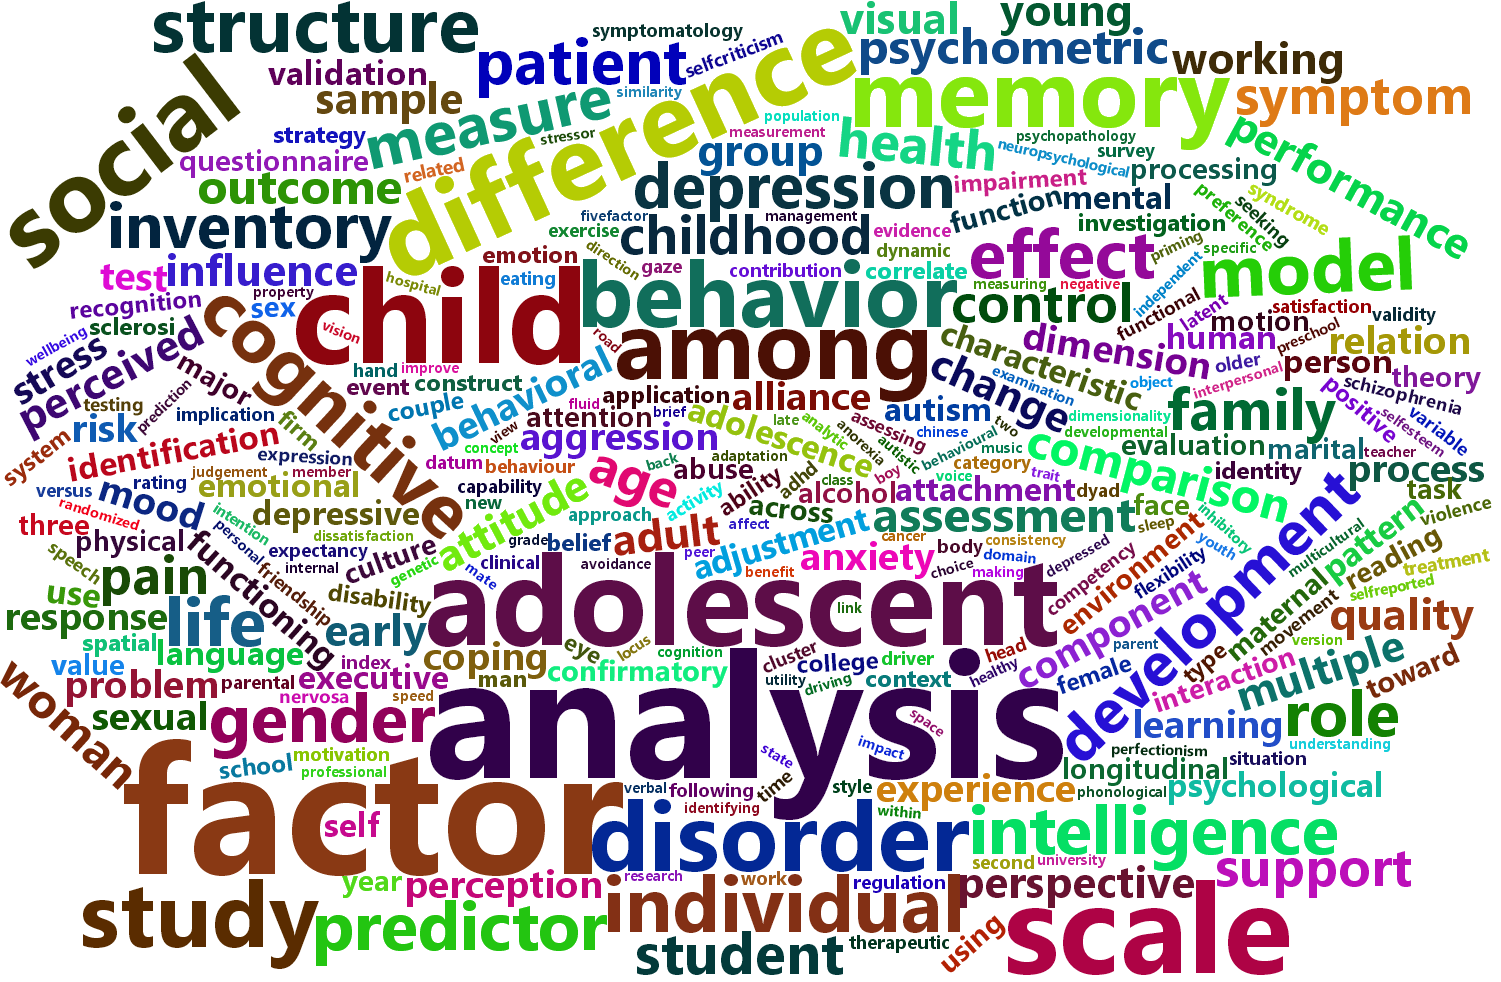
\includegraphics[width=0.7\linewidth,height=\textheight,keepaspectratio]{images/wordcloud4.png}

}

\caption{\label{fig-wordcloud}Wordcloud illustrating the topic content
of the articles in the bibliographic database, showing the 50 most
frequently-used, with font size proportional to frequency.}

\end{figure}%

\section{Linear models: Univariate to
multivariate}\label{linear-models-univariate-to-multivariate}

The path to multivariate thinking in this book is eased by the
simplicity of extending univariate models to multivariate ones in
notation and computation. For classical linear models for ANOVA and
regression, the step from a univariate model for a single response,
\(y\), to a multivariate one for a collection of \(p\) responses,
\(\mathbf{y}\) is conceptually very easy. That's because the univariate
model with \(q\) predictors,

\[y_i = \beta_0 + \beta_1 x_1 + \beta_2 x_2 + \dots + \beta_q x_q + \epsilon_i \;, \]

when cast in matrix terms,

\[
\mathbf{y} = \mathbf{X} \; \boldsymbol{\beta} + \boldsymbol{\epsilon}\;, \quad\mbox{   with   }\quad \boldsymbol{\epsilon} \sim \mathcal{N} (0, \sigma^2 \mathbf{I}) \;,
\]

generalizes directly to an analogous multivariate linear model (MLM),

\[
\mathbf{Y} = [\mathbf{y_1}, \mathbf{y_2}, \dots, \mathbf{y_p}] = \mathbf{X} \; \mathbf{B} + \boldsymbol{\Large\varepsilon}\quad\mbox{   with   }\quad \boldsymbol{\Large\varepsilon}\sim \mathcal{N} (\mathbf{0}, \boldsymbol{\Sigma}) \; ,
\]

for multiple responses (as will be discussed in detail in
Chapter~\ref{sec-mlm-review}). The design matrix, \(\mathbf{X}\) remains
the same, and the vector \(\beta\) of coefficients simply becomes a
matrix \(\mathbf{B}\), with one column for each of the \(p\) outcome
variables.

Computationally, all of these are handled by a single R function,
\texttt{lm()} \ixfunc{lm()} . Methods for the resulting \texttt{"lm"}
objects (also of class \texttt{mlm"} for the multivariate case) provide
general means for analysis and graphics and have been developed widely
in various R packages.

Happily as well, hypothesis tests for the MLM are also straight-forward
generalizations of the familiar \(F\) and \(t\)-tests for univariate
response models. Moreover, there is a rich geometry underlying these
generalizations (\citeproc{ref-Friendly-etal:ellipses:2013}{Friendly et
al., 2013}) which we can exploit for understanding and visualization in
Chapter~\ref{sec-vis-mlm}.

\section{Visualization is harder}\label{visualization-is-harder}

However, with two or more response variables, visualizations for
multivariate models are not as simple as they are for their univariate
counterparts. These include plots for understanding the data at hand,
the effects of predictors, model parameters, or model diagnostics.

Consequently, the results of such studies are often explored and
discussed solely in terms of coefficients and significance, and
visualizations of the relationships are only provided for one response
variable at a time, if at all. This tradition can mask important
nuances, and lead researchers to draw erroneous conclusions.

The aim of this book is to describe and illustrate some central methods
that we have developed over the last thirty years that aid in the
understanding and communication of the results of multivariate models
(\citeproc{ref-Friendly:94a}{Friendly, 1994},
\citeproc{ref-Friendly:02:corrgram}{2002},
\citeproc{ref-Friendly-07-manova}{2007};
\citeproc{ref-FriendlyMeyer:2016:DDAR}{Friendly \& Meyer, 2016}). These
methods for quantitative data rely on \emph{data ellipsoids} as simple,
minimally sufficient visualizations of variance that can be shown in 2D
and 3D plots. As will be demonstrated, the \emph{Hypothesis-Error (HE)
plot} framework (Section~\ref{sec-he-framework}) applies this idea to
the results of multivariate tests of linear hypotheses.
\index{data ellipse} \index{HE plot}

Further, in the case where there are more than just a few outcome
variables, the important nectar of their relationships to predictors can
often be distilled in a \emph{multivariate juicer}--- a
\textbf{projection} of the multivariate relationships to the predictors
in the low-D space that captures most of the flavor. This idea can be
applied using \emph{animated tours} of high-D data
(Section~\ref{sec-animated-tours}), principal components analysis and
\emph{biplots} (Section~\ref{sec-biplot}) \emph{canonical correlation
plots} and with \emph{canonical discriminant HE plots}
(Section~\ref{sec-candisc}). \index{principal components analysis}
\index{canonical correlation} \index{projection}

A glimpse of this idea can be seen in Figure~\ref{fig-cover-GBE}, the
cover image from Douglas Hofstadter's \emph{Gödel, Bach and Escher}
(\citeproc{ref-Hofstadter1979}{1979}). The complete image in 3D is made
up of two 3D solids, with various complicated cutouts and holes. Each 2D
view of this is the shadow, or projection shown on the walls. These 2D
views capture some salient aspects of the complete 3D scene, but as in
the case of the \emph{Flatlander} Square trying to understand the
Sphere, it takes some imagination to get there. The methods of this book
are designed to expand your understanding of relationships in
higher-dimensional data.

\begin{figure}[htb!]

\centering{

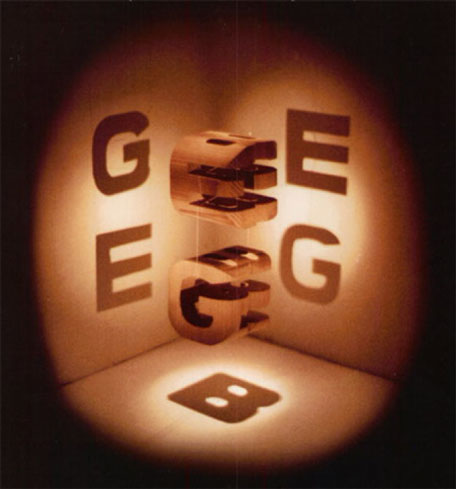
\includegraphics[width=0.6\linewidth,height=\textheight,keepaspectratio]{images/Cover-GBE.png}

}

\caption{\label{fig-cover-GBE}\textbf{Projection}: The cover image from
Douglas Hofstadter's \emph{Gödel, Bach and Escher}
(\citeproc{ref-Hofstadter1979}{1979}) illustrates projection of 3D
solids onto each 2D plane. Each 2D view captures some salient aspect of
the complete figure, but is incomplete.}

\end{figure}%

\section{Problems in understanding and communicating MLM
results}\label{sec-problems}

In my consulting practice within the Statistical Consulting Service at
York University, I see hundreds of clients each year ranging from
advanced undergraduate thesis students, to graduate students and faculty
from a variety of fields. Initially, most clients used SAS or SPSS, but
now most use R or Stata for their analyses.

Over the last three decades, and across these groups, I have noticed an
increasing desire to utilize multivariate methods. As researchers are
exposed to the utility and power of multivariate tests, they see them as
an appealing alternative to running many univariate ANOVAs or multiple
regressions for each response variable separately.

However, multivariate analyses are more complicated than such
approaches, especially when it comes to understanding and communicating
results. Output is typically voluminous, and researchers will often get
lost in the numbers. While software in SAS, SPSS and R make tabular
summary displays relatively easy, these often obscure the findings that
researchers are most interested in. The most common analytic oversights
that I have observed are:

\begin{itemize}
\item
  \textbf{Atomistic model checking}: Researchers have mostly learned the
  assumptions (the Holy Trinity of normality, constant variance and
  independence) of univariate linear models, but then apply
  \emph{univariate} tests (e.g., Shapiro-Wilk) and diagnostic plots
  (normal QQ plots) to every predictor and every response. Instead, I
  recommend more comprehensive graphical methods like scale-location and
  influence plots (Section~\ref{sec-diagnostic-plots}) and plots like
  chi-square QQ plots (Section~\ref{sec-model-diagnostics-MLM}) for
  multivariate models.
\item
  \textbf{Bonferroni everywhere}: Faced with the task of reporting the
  results for multiple response measures and a collection of predictors
  for each, a common tendency is to run (and sometimes report) each of
  the separate univariate response models and then apply a correction
  for multiple testing. Not only is this confusing and awkward to
  report, but it is largely unnecessary because the multivariate tests
  provide protection for multiple testing. Instead, I emphasize thinking
  about \emph{substantive} questions concerning differences among groups
  and testing these with \emph{contrasts} (Section~\ref{sec-contrasts})
  and \emph{linear hypotheses} (Section~\ref{sec-contrasts2}).
\item
  \textbf{Reverting to univariate visualizations}: To display results,
  some software makes some visualization methods available through menu
  choices or syntax, but usually these are the wrong (or at least
  unhelpful) choices, in that they generate separate univariate graphs
  for the individual responses.
\end{itemize}

This book discusses a few essential procedures for multivariate linear
models, how their interpretation can be aided through the use of
well-crafted (though novel) visualizations, and provides replicable
sample code in R to showcase their use in applied behavioral research.

\chapter{Getting Started}\label{sec-getting_started}

\begin{quote}
\emph{Getting information from a table is like extracting sunlight from
a cucumber.} ---Farquhar \& Farquhar
(\citeproc{ref-FarquharFarquhar:91}{1891})
\end{quote}

At the time the Farhquhar brothers wrote this pithy aphorism, graphical
methods for understanding data had advanced considerably, but most
statisticians still relied on tables to their communicate results,
prompting their complaint. Most data tables we see today are designed
for looking something up like the number of measles cases in Ontario
compared to other provinces. Tables are not usually designed to reveal
\emph{patterns, trends or anomalies}, although this can be accomplished
with modern table generating software such as the
\textcolor{brown}{\texttt{\textbf{tinytable}}} %
   \index{tinytable@\texttt{tinytable} package}%
   \index{packages!tinytable@\texttt{tinytable}}%
     or \textcolor{brown}{\texttt{\textbf{gt}}} %
   \index{gt@\texttt{gt} package}%
   \index{packages!gt@\texttt{gt}}%
     packages.\footnote{For example, a cell in a table can be used to
  show a ``sparklines'' (Tufte (\citeproc{ref-Tufte:83}{1983})), tiny
  versions of a line graph or bar chart. As well, table rows and/or
  columns can be sorted to show trends or background colors can be used
  to show unusual values.}

The main graphic forms we use today---the pie chart, line graphs and
bar---were invented by William Playfair around 1800
(\citeproc{ref-Playfair:1786}{Playfair, 1786},
\citeproc{ref-Playfair:1801}{1801}). The scatterplot arrived shortly
after (\citeproc{ref-Herschel:1833}{Herschel, 1833}) and thematic maps
showing the spatial distributions of social variables (crime, suicides,
literacy) were used for the first time to reason about important
societal questions (\citeproc{ref-Guerry:1833}{Guerry, 1833}) such as
``is increased education associated with lower rates of crime?''
\index{pie chart} \index{bar chart} \index{line graph}
\index{scatterplot}

In the last half of the 18th Century, the idea of correlation was
developed (\citeproc{ref-Galton:1886}{Galton, 1886};
\citeproc{ref-Pearson:1896}{Pearson, 1896}) and the period, roughly
1860--1890, dubbed the ``Golden Age of Graphics''
(\citeproc{ref-Friendly:2008:golden}{Friendly, 2008};
\citeproc{ref-Funkhouser:1937}{Funkhouser, 1937}) became the richest
period of innovation and beauty in the entire history of data
visualization. During this time there was an incredible development of
\emph{visual thinking}, represented by the work of Charles Joseph
Minard, advances in the role of visualization within scientific
discovery, as illustrated through Francis Galton, and graphical
excellence, embodied in state statistical atlases produced in France and
elsewhere. See Friendly (\citeproc{ref-Friendly:2008:golden}{2008});
Friendly \& Wainer (\citeproc{ref-FriendlyWainer:2021:TOGS}{2021}) for
this history. \index{visual thinking}.

\section{Why plot your data?}\label{sec-why_plot}

This chapter introduces the importance of graphing data through three
nearly classic stories with the following themes:

\begin{itemize}
\item
  \textbf{summary statistics are not enough}: Anscombe's Quartet
  demonstrates datasets that are indistinguishable by numerical summary
  statistics (mean, standard deviation, correlation), but whose
  relationships are vastly different.
\item
  \textbf{one lousy point can ruin your day}: A researcher is mystified
  by a difference between a correlation for men and women until she
  plots the data.
\item
  \textbf{finding the signal in noise}: The story of the US 1970 Draft
  Lottery shows how a weak, but reliable signal, reflecting bias in a
  process can be revealed by graphical enhancement and summarization.
\end{itemize}

\subsection{Anscombe's Quartet}\label{sec-anscombe}

In 1973, Francis Anscombe (\citeproc{ref-Anscombe:73}{Anscombe, 1973})
famously constructed a set of four datasets illustrate the importance of
plotting the graphs before analyzing and model building, and the effect
of unusual observations on fitted models. Now known as \emph{Anscombe's
Quartet}, these datasets had identical statistical properties: the same
means, standard deviations, correlations and regression lines.
\index{Anscombe's quartet} \index{quartet!Anscombe}

His purpose was to debunk three notions that had been prevalent at the
time:

\begin{itemize}
\tightlist
\item
  Numerical calculations are exact, but graphs are coarse and limited by
  perception and resolution;
\item
  For any particular kind of statistical data there is just one set of
  calculations constituting a correct statistical analysis;
\item
  Performing intricate calculations is virtuous, whereas actually
  looking at the data is cheating.
\end{itemize}

The dataset \texttt{datasets::anscombe}
\index{anscombe@\texttt{anscombe} data}
\index{datasets!anscombe@\texttt{anscombe}}
\index{datasets@\texttt{datasets} package}
\index{packages!datasets@\texttt{datasets}} has 11 observations,
recorded in wide format, with variables \texttt{x1:x4} and
\texttt{y1:y4}.

\begin{Shaded}
\begin{Highlighting}[]
\FunctionTok{data}\NormalTok{(anscombe) }
\FunctionTok{head}\NormalTok{(anscombe)}
\CommentTok{\#   x1 x2 x3 x4   y1   y2    y3   y4}
\CommentTok{\# 1 10 10 10  8 8.04 9.14  7.46 6.58}
\CommentTok{\# 2  8  8  8  8 6.95 8.14  6.77 5.76}
\CommentTok{\# 3 13 13 13  8 7.58 8.74 12.74 7.71}
\CommentTok{\# 4  9  9  9  8 8.81 8.77  7.11 8.84}
\CommentTok{\# 5 11 11 11  8 8.33 9.26  7.81 8.47}
\CommentTok{\# 6 14 14 14  8 9.96 8.10  8.84 7.04}
\end{Highlighting}
\end{Shaded}

The following code transforms this data to long format and calculates
some summary statistics for each \texttt{dataset}.

\begin{Shaded}
\begin{Highlighting}[]
\NormalTok{anscombe\_long }\OtherTok{\textless{}{-}}\NormalTok{ anscombe }\SpecialCharTok{|\textgreater{}} 
  \FunctionTok{pivot\_longer}\NormalTok{(}\FunctionTok{everything}\NormalTok{(), }
               \AttributeTok{names\_to =} \FunctionTok{c}\NormalTok{(}\StringTok{".value"}\NormalTok{, }\StringTok{"dataset"}\NormalTok{), }
               \AttributeTok{names\_pattern =} \StringTok{"(.)(.)"}
\NormalTok{  ) }\SpecialCharTok{|\textgreater{}}
  \FunctionTok{arrange}\NormalTok{(dataset)}

\NormalTok{anscombe\_long }\SpecialCharTok{|\textgreater{}}
  \FunctionTok{group\_by}\NormalTok{(dataset) }\SpecialCharTok{|\textgreater{}}
  \FunctionTok{summarise}\NormalTok{(}\AttributeTok{xbar      =} \FunctionTok{mean}\NormalTok{(x),}
            \AttributeTok{ybar      =} \FunctionTok{mean}\NormalTok{(y),}
            \AttributeTok{r         =} \FunctionTok{cor}\NormalTok{(x, y),}
            \AttributeTok{intercept =} \FunctionTok{coef}\NormalTok{(}\FunctionTok{lm}\NormalTok{(y }\SpecialCharTok{\textasciitilde{}}\NormalTok{ x))[}\DecValTok{1}\NormalTok{],}
            \AttributeTok{slope     =} \FunctionTok{coef}\NormalTok{(}\FunctionTok{lm}\NormalTok{(y }\SpecialCharTok{\textasciitilde{}}\NormalTok{ x))[}\DecValTok{2}\NormalTok{]}
\NormalTok{         )}
\CommentTok{\# \# A tibble: 4 x 6}
\CommentTok{\#   dataset  xbar  ybar     r intercept slope}
\CommentTok{\#   \textless{}chr\textgreater{}   \textless{}dbl\textgreater{} \textless{}dbl\textgreater{} \textless{}dbl\textgreater{}     \textless{}dbl\textgreater{} \textless{}dbl\textgreater{}}
\CommentTok{\# 1 1           9  7.50 0.816      3.00 0.500}
\CommentTok{\# 2 2           9  7.50 0.816      3.00 0.5  }
\CommentTok{\# 3 3           9  7.5  0.816      3.00 0.500}
\CommentTok{\# 4 4           9  7.50 0.817      3.00 0.500}
\end{Highlighting}
\end{Shaded}

As we can see, all four datasets have nearly identical univariate and
bivariate statistical measures. You can only see how they differ in
graphs, which show their true natures to be vastly different.

Figure~\ref{fig-anscombe1} is an enhanced version of Anscombe's plot of
these data, adding helpful annotations to show visually the underlying
statistical summaries.

\begin{figure}[htb!]

\centering{

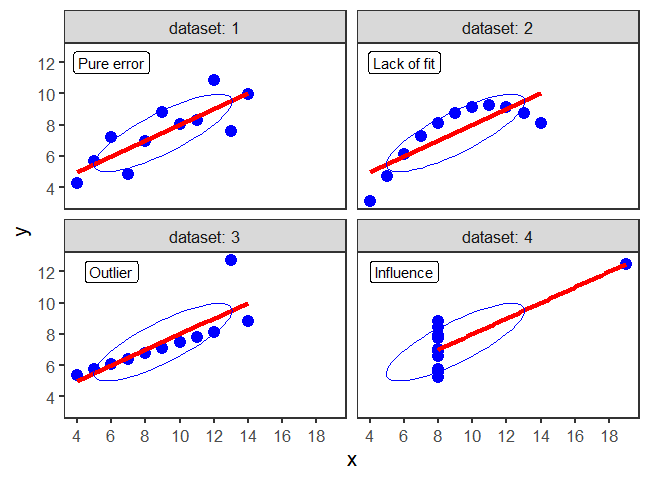
\includegraphics[width=0.9\linewidth,height=\textheight,keepaspectratio]{images/anscombe1.png}

}

\caption{\label{fig-anscombe1}Scatterplots of Anscombe's Quartet. Each
plot shows the fitted regression line and a 68\% data ellipse
representing the correlation between \(x\) and \(y\).}

\end{figure}%

This figure is produced as follows, using a single call to
\texttt{ggplot()} \ixfunc{ggplot()} , faceted by \texttt{dataset}. As we
will see later (Section~\ref{sec-data-ellipse}), the data ellipse
(produced by \texttt{stat\_ellipse()}) reflects the correlation between
the variables. \index{data ellipse}
\index{stat_ellipse()@\texttt{stat\_ellipse()}}

\begin{Shaded}
\begin{Highlighting}[]
\NormalTok{desc }\OtherTok{\textless{}{-}} \FunctionTok{tibble}\NormalTok{(}
  \AttributeTok{dataset =} \DecValTok{1}\SpecialCharTok{:}\DecValTok{4}\NormalTok{,}
  \AttributeTok{label =} \FunctionTok{c}\NormalTok{(}\StringTok{"Pure error"}\NormalTok{, }\StringTok{"Lack of fit"}\NormalTok{, }\StringTok{"Outlier"}\NormalTok{, }\StringTok{"Influence"}\NormalTok{)}
\NormalTok{)}

\FunctionTok{ggplot}\NormalTok{(anscombe\_long, }\FunctionTok{aes}\NormalTok{(}\AttributeTok{x =}\NormalTok{ x, }\AttributeTok{y =}\NormalTok{ y)) }\SpecialCharTok{+}
  \FunctionTok{geom\_point}\NormalTok{(}\AttributeTok{color =} \StringTok{"blue"}\NormalTok{, }\AttributeTok{size =} \DecValTok{4}\NormalTok{) }\SpecialCharTok{+}
  \FunctionTok{geom\_smooth}\NormalTok{(}\AttributeTok{method =} \StringTok{"lm"}\NormalTok{, }\AttributeTok{formula =}\NormalTok{ y }\SpecialCharTok{\textasciitilde{}}\NormalTok{ x, }\AttributeTok{se =} \ConstantTok{FALSE}\NormalTok{,}
              \AttributeTok{color =} \StringTok{"red"}\NormalTok{, }\AttributeTok{linewidth =} \FloatTok{1.5}\NormalTok{) }\SpecialCharTok{+}
  \FunctionTok{scale\_x\_continuous}\NormalTok{(}\AttributeTok{breaks =} \FunctionTok{seq}\NormalTok{(}\DecValTok{0}\NormalTok{,}\DecValTok{20}\NormalTok{,}\DecValTok{2}\NormalTok{)) }\SpecialCharTok{+}
  \FunctionTok{scale\_y\_continuous}\NormalTok{(}\AttributeTok{breaks =} \FunctionTok{seq}\NormalTok{(}\DecValTok{0}\NormalTok{,}\DecValTok{12}\NormalTok{,}\DecValTok{2}\NormalTok{)) }\SpecialCharTok{+}
  \FunctionTok{stat\_ellipse}\NormalTok{(}\AttributeTok{level =} \FloatTok{0.5}\NormalTok{, }\AttributeTok{color=}\NormalTok{col, }\AttributeTok{type=}\StringTok{"norm"}\NormalTok{) }\SpecialCharTok{+}
  \FunctionTok{geom\_label}\NormalTok{(}\AttributeTok{data=}\NormalTok{desc, }\FunctionTok{aes}\NormalTok{(}\AttributeTok{label =}\NormalTok{ label), }\AttributeTok{x=}\DecValTok{6}\NormalTok{, }\AttributeTok{y=}\DecValTok{12}\NormalTok{) }\SpecialCharTok{+}
  \FunctionTok{facet\_wrap}\NormalTok{(}\SpecialCharTok{\textasciitilde{}}\NormalTok{dataset, }\AttributeTok{labeller =}\NormalTok{ label\_both) }
\end{Highlighting}
\end{Shaded}

The subplots are labeled with the statistical idea they reflect:

\begin{itemize}
\item
  dataset 1: \textbf{Pure error}. This is the typical case with
  well-behaved data. Variation of the points around the line reflect
  only measurement error or unreliability in the response, \(y\).
  \index{pure error}
\item
  dataset 2: \textbf{Lack of fit}. The data is clearly curvilinear, and
  would be very well described by a quadratic,
  \texttt{y\ \textasciitilde{}\ poly(x,\ 2)}. This violates the
  assumption of linear regression that the fitted model has the correct
  form. \index{lack of fit}
\item
  dataset 3: \textbf{Outlier}. One point, second from the right, has a
  very large residual. Because this point is near the extreme of \(x\),
  it pulls the regression line towards it, as you can see by imagining a
  line through the remaining points. \index{outliers}
\item
  dataset 4: \textbf{Influence}. All but one of the points have the same
  \(x\) value. The one unusual point has sufficient influence to force
  the regression line to fit it \textbf{exactly}. \index{influence}
\end{itemize}

One moral from this example:

\begin{quote}
\textbf{Linear regression only ``sees'' a line. It does its' best when
the data are really linear. Because the line is fit by least squares, it
pulls the line toward discrepant points to minimize the sum of squared
residuals.}
\end{quote}

\begin{tcolorbox}[enhanced jigsaw, titlerule=0mm, bottomtitle=1mm, left=2mm, opacityback=0, bottomrule=.15mm, breakable, colframe=quarto-callout-note-color-frame, toptitle=1mm, rightrule=.15mm, opacitybacktitle=0.6, colbacktitle=quarto-callout-note-color!10!white, leftrule=.75mm, coltitle=black, arc=.35mm, title=\textcolor{quarto-callout-note-color}{\faInfo}\hspace{0.5em}{Datasaurus Dozen}, toprule=.15mm, colback=white]

The method Anscombe used to compose his quartet is unknown, but it turns
out that that there is a method to construct a wider collection of
datasets with identical statistical properties. After all, in a
bivariate dataset with \(n\) observations, the correlation has \((n-2)\)
degrees of freedom, so it is possible to choose \(n-2\) of the
\((x, y)\) pairs to yield any given value. As it happens, it is also
possible to create any number of datasets with the same means, standard
deviations and correlations with nearly any shape you like --- even a
dinosaur! \index{datasaurus dozen}

The \emph{Datasaurus Dozen} was first publicized by Alberto Cairo in a
\href{http://www.thefunctionalart.com/2016/08/download-datasaurus-never-trust-summary.html}{blog
post} and are available in the
\textcolor{brown}{\texttt{\textbf{datasauRus}}} package
(\citeproc{ref-R-datasauRus}{Gillespie et al., 2025}) %
   \index{datasauRus@\texttt{datasauRus} package}%
   \index{packages!datasauRus@\texttt{datasauRus}}%
     . As shown in Figure~\ref{fig-datasaurus-pdf} the sets include a
star, cross, circle, bullseye, horizontal and vertical lines, and, of
course the ``dino''. The method
(\citeproc{ref-MatejkaFitzmaurice2017}{Matejka \& Fitzmaurice, 2017})
uses \emph{simulated annealing}, an iterative process that perturbs the
points in a scatterplot, moving them towards a given shape while keeping
the statistical summaries close to the fixed target value.

The \textcolor{brown}{\texttt{\textbf{datasauRus}}} %
   \index{datasauRus@\texttt{datasauRus} package}%
   \index{packages!datasauRus@\texttt{datasauRus}}%
     package just contains the datasets, but a general method, called
\emph{statistical metamers}, for producing such datasets has been
described by
\href{https://eliocamp.github.io/codigo-r/en/2019/01/statistical-metamerism/}{Elio
Campitelli} and implemented in the
\textcolor{brown}{\texttt{\textbf{metamer}}} %
   \index{metamer@\texttt{metamer} package}%
   \index{packages!metamer@\texttt{metamer}}%
     package.

\end{tcolorbox}

\begin{figure}[htb!]

\centering{

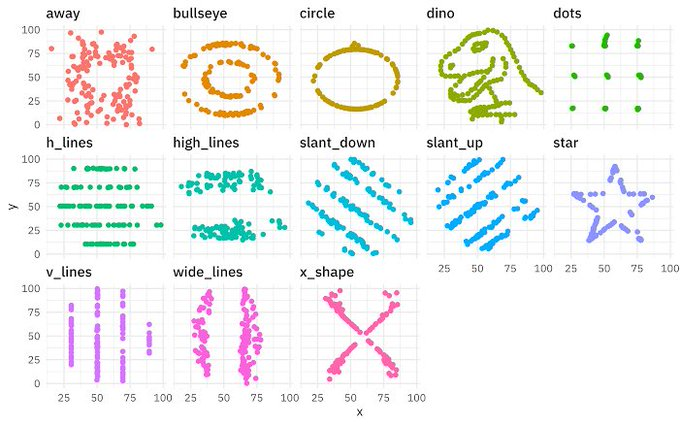
\includegraphics[width=1\linewidth,height=\textheight,keepaspectratio]{images/datasaurus-dozen.jpg}

}

\caption{\label{fig-datasaurus-pdf}Plots of the Dinosaur Dozen datasets.
\emph{Source}:
\href{https://x.com/selcukorkmaz/status/1864583253253927156}{Selçuk
Korkmaz on X}}

\end{figure}%

\begin{tcolorbox}[enhanced jigsaw, titlerule=0mm, bottomtitle=1mm, left=2mm, opacityback=0, bottomrule=.15mm, breakable, colframe=quarto-callout-note-color-frame, toptitle=1mm, rightrule=.15mm, opacitybacktitle=0.6, colbacktitle=quarto-callout-note-color!10!white, leftrule=.75mm, coltitle=black, arc=.35mm, title=\textcolor{quarto-callout-note-color}{\faInfo}\hspace{0.5em}{Quartets}, toprule=.15mm, colback=white]

The essential idea of a statistical ``quartet'' is to illustrate four
quite different datasets or circumstances that seem superficially the
same, but yet are paradoxically very different when you look behind the
scenes.

For example, in the context of causal analysis Gelman et al.
(\citeproc{ref-Gelman-etal:2023}{2023}), illustrated sets of four
graphs, within each of which all four represent the same average
(latent) causal effect but with much different patterns of individual
effects. McGowan et al. (\citeproc{ref-McGowan2023}{2023}) provide
another illustration with four seemingly identical data sets each
generated by a different causal mechanism. \index{causal analysis}

As an example of machine learning models, Biecek et al.
(\citeproc{ref-Biecek-etal:2023}{2023}), introduced the ``Rashamon
Quartet'', a synthetic dataset for which four models from different
classes (linear model, regression tree, random forest, neural network)
have practically identical predictive performance. In all cases, the
paradox is solved when their visualization reveals the distinct ways of
understanding structure in the data. The
\textcolor{brown}{\texttt{\textbf{quartets}}} package
(\citeproc{ref-R-quartets}{D'Agostino McGowan, 2023}) %
   \index{quartets@\texttt{quartets} package}%
   \index{packages!quartets@\texttt{quartets}}%
     contains these and other variations on this theme.
\index{quartet!causal} \index{quartet!Rashamon}

\end{tcolorbox}

\subsection{One lousy point can ruin your day}\label{sec-davis}

In the mid 1980s, a consulting client had a strange problem.\footnote{This
  story is told apocryphally. The consulting client actually did plot
  the data, but needed help in understanding what went wrong in her
  analyses and in making better graphs.} She was conducting a study of
the relation between body image and weight preoccupation in exercising
and non-exercising people (\citeproc{ref-Davis:1990}{Davis, 1990}). As
part of the design, the researcher wanted to know if self-reported
weight could be taken as a reliable indicator of true weight measured on
a scale. It was expected that the correlations between reported and
measured weight should be close to 1.0, and the slope of the regression
lines for men and women should also be close to 1.0. The dataset is
\texttt{carData::Davis} \index{Davis@\texttt{Davis} data}
\index{datasets!Davis@\texttt{Davis}}
\index{carData@\texttt{carData} package}
\index{packages!carData@\texttt{carData}}.

She was therefore very surprised to see the following numerical results:
For men, the correlation was nearly perfect, but not so for women.

\begin{Shaded}
\begin{Highlighting}[]
\FunctionTok{data}\NormalTok{(Davis, }\AttributeTok{package=}\StringTok{"carData"}\NormalTok{)}
\NormalTok{Davis }\OtherTok{\textless{}{-}}\NormalTok{ Davis }\SpecialCharTok{|\textgreater{}}
  \FunctionTok{drop\_na}\NormalTok{()          }\CommentTok{\# drop missing cases}
\NormalTok{Davis }\SpecialCharTok{|\textgreater{}}
  \FunctionTok{group\_by}\NormalTok{(sex) }\SpecialCharTok{|\textgreater{}}
  \FunctionTok{select}\NormalTok{(sex, weight, repwt) }\SpecialCharTok{|\textgreater{}}
  \FunctionTok{summarise}\NormalTok{(}\AttributeTok{r =} \FunctionTok{cor}\NormalTok{(weight, repwt))}
\CommentTok{\# \# A tibble: 2 x 2}
\CommentTok{\#   sex       r}
\CommentTok{\#   \textless{}fct\textgreater{} \textless{}dbl\textgreater{}}
\CommentTok{\# 1 F     0.501}
\CommentTok{\# 2 M     0.979}
\end{Highlighting}
\end{Shaded}

Similarly, the regression lines showed the expected slope for men, but
that for women was only 0.26.

\begin{Shaded}
\begin{Highlighting}[]
\NormalTok{Davis }\SpecialCharTok{|\textgreater{}}
  \FunctionTok{nest}\NormalTok{(}\AttributeTok{data =} \SpecialCharTok{{-}}\NormalTok{sex) }\SpecialCharTok{|\textgreater{}}
  \FunctionTok{mutate}\NormalTok{(}\AttributeTok{model =} \FunctionTok{map}\NormalTok{(data, }\SpecialCharTok{\textasciitilde{}} \FunctionTok{lm}\NormalTok{(repwt }\SpecialCharTok{\textasciitilde{}}\NormalTok{ weight, }\AttributeTok{data =}\NormalTok{ .)),}
         \AttributeTok{tidied =} \FunctionTok{map}\NormalTok{(model, tidy)) }\SpecialCharTok{|\textgreater{}}
  \FunctionTok{unnest}\NormalTok{(tidied) }\SpecialCharTok{|\textgreater{}}
  \FunctionTok{filter}\NormalTok{(term }\SpecialCharTok{==} \StringTok{"weight"}\NormalTok{) }\SpecialCharTok{|\textgreater{}}
  \FunctionTok{select}\NormalTok{(sex, term, estimate, std.error)}
\CommentTok{\# \# A tibble: 2 x 4}
\CommentTok{\#   sex   term   estimate std.error}
\CommentTok{\#   \textless{}fct\textgreater{} \textless{}chr\textgreater{}     \textless{}dbl\textgreater{}     \textless{}dbl\textgreater{}}
\CommentTok{\# 1 M     weight    0.990    0.0229}
\CommentTok{\# 2 F     weight    0.262    0.0459}
\end{Highlighting}
\end{Shaded}

``What could be wrong here?'', the client asked. The consultant replied
with the obvious question:

\begin{quote}
\emph{\textbf{Did you plot your data?}}
\end{quote}

The answer turned out to be one discrepant point, a female (case 12),
whose measured weight was 166 kg (366 lbs!). This single point exerted
so much influence that it pulled the fitted regression line down to a
slope of only 0.26. \index{influence}

\begin{Shaded}
\begin{Highlighting}[]
\CommentTok{\# shorthand to position legend inside the figure}
\NormalTok{legend\_inside }\OtherTok{\textless{}{-}} \ControlFlowTok{function}\NormalTok{(position) \{          }\CommentTok{\# simplify legend placement}
  \FunctionTok{theme}\NormalTok{(}\AttributeTok{legend.position =} \StringTok{"inside"}\NormalTok{,}
        \AttributeTok{legend.position.inside =}\NormalTok{ position)}
\NormalTok{\}}

\NormalTok{Davis }\SpecialCharTok{|\textgreater{}}
  \FunctionTok{ggplot}\NormalTok{(}\FunctionTok{aes}\NormalTok{(}\AttributeTok{x =}\NormalTok{ weight, }\AttributeTok{y =}\NormalTok{ repwt, }
             \AttributeTok{color =}\NormalTok{ sex, }\AttributeTok{shape =}\NormalTok{ sex, }\AttributeTok{linetype =}\NormalTok{ sex)) }\SpecialCharTok{+}
  \FunctionTok{geom\_point}\NormalTok{(}\AttributeTok{size =} \FunctionTok{ifelse}\NormalTok{(Davis}\SpecialCharTok{$}\NormalTok{weight}\SpecialCharTok{==}\DecValTok{166}\NormalTok{, }\DecValTok{6}\NormalTok{, }\DecValTok{2}\NormalTok{)) }\SpecialCharTok{+}
  \FunctionTok{geom\_smooth}\NormalTok{(}\AttributeTok{method =} \StringTok{"lm"}\NormalTok{, }\AttributeTok{formula =}\NormalTok{ y}\SpecialCharTok{\textasciitilde{}}\NormalTok{x, }\AttributeTok{se =} \ConstantTok{FALSE}\NormalTok{) }\SpecialCharTok{+}
  \FunctionTok{labs}\NormalTok{(}\AttributeTok{x =} \StringTok{"Measured weight (kg)"}\NormalTok{, }
       \AttributeTok{y =} \StringTok{"Reported weight (kg)"}\NormalTok{) }\SpecialCharTok{+}
  \FunctionTok{scale\_linetype\_manual}\NormalTok{(}\AttributeTok{values =} \FunctionTok{c}\NormalTok{(}\AttributeTok{F =} \StringTok{"longdash"}\NormalTok{, }
                                   \AttributeTok{M =} \StringTok{"solid"}\NormalTok{)) }\SpecialCharTok{+}
  \FunctionTok{legend\_inside}\NormalTok{(}\FunctionTok{c}\NormalTok{(.}\DecValTok{8}\NormalTok{, .}\DecValTok{8}\NormalTok{))}
\end{Highlighting}
\end{Shaded}

\begin{figure}[htb!]

\centering{

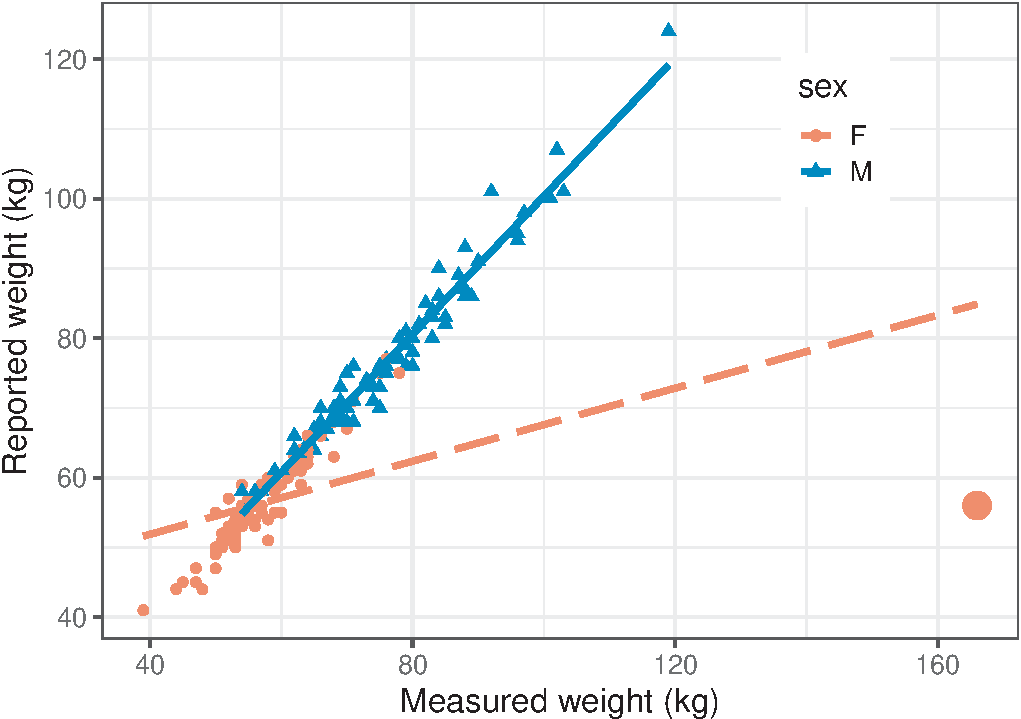
\includegraphics[width=0.7\linewidth,height=\textheight,keepaspectratio]{figs/ch03/fig-davis-reg1-1.pdf}

}

\caption{\label{fig-davis-reg1}Regression for Davis' data on reported
weight and measures weight for men and women. Separate regression lines,
predicting reported weight from measured weight are shown for males and
females. One highly unusual point is highlighted.}

\end{figure}%

In this example, it was arguable that \(x\) and \(y\) axes should be
reversed, to determine how well measured weight can be predicted from
reported weight. In \texttt{ggplot} this can easily be done by reversing
the \texttt{x} and \texttt{y} aesthetics.

\begin{Shaded}
\begin{Highlighting}[]
\NormalTok{Davis }\SpecialCharTok{|\textgreater{}}
  \FunctionTok{ggplot}\NormalTok{(}\FunctionTok{aes}\NormalTok{(}\AttributeTok{y =}\NormalTok{ weight, }\AttributeTok{x =}\NormalTok{ repwt, }\AttributeTok{color =}\NormalTok{ sex, }\AttributeTok{shape=}\NormalTok{sex)) }\SpecialCharTok{+}
  \FunctionTok{geom\_point}\NormalTok{(}\AttributeTok{size =} \FunctionTok{ifelse}\NormalTok{(Davis}\SpecialCharTok{$}\NormalTok{weight}\SpecialCharTok{==}\DecValTok{166}\NormalTok{, }\DecValTok{6}\NormalTok{, }\DecValTok{2}\NormalTok{)) }\SpecialCharTok{+}
  \FunctionTok{labs}\NormalTok{(}\AttributeTok{y =} \StringTok{"Measured weight (kg)"}\NormalTok{, }
       \AttributeTok{x =} \StringTok{"Reported weight (kg)"}\NormalTok{) }\SpecialCharTok{+}
    \FunctionTok{geom\_smooth}\NormalTok{(}\AttributeTok{method =} \StringTok{"lm"}\NormalTok{, }\AttributeTok{formula =}\NormalTok{ y}\SpecialCharTok{\textasciitilde{}}\NormalTok{x, }\AttributeTok{se =} \ConstantTok{FALSE}\NormalTok{) }\SpecialCharTok{+}
  \FunctionTok{legend\_inside}\NormalTok{(}\FunctionTok{c}\NormalTok{(.}\DecValTok{8}\NormalTok{, .}\DecValTok{8}\NormalTok{))}
\end{Highlighting}
\end{Shaded}

\begin{figure}[htb!]

\centering{

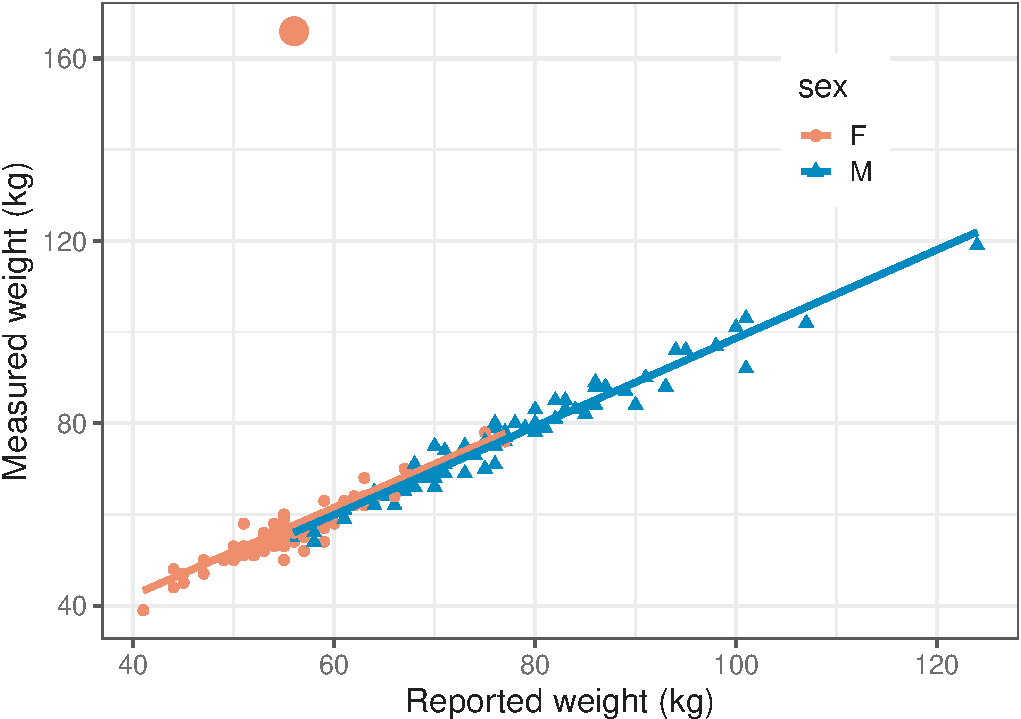
\includegraphics[width=0.7\linewidth,height=\textheight,keepaspectratio]{figs/ch03/fig-davis-reg2-1.pdf}

}

\caption{\label{fig-davis-reg2}Regression for Davis' data on reported
weight and measures weight for men and women. Separate regression lines,
predicting measured weight from reported weight are shown for males and
females. The highly unusual point no longer has an effect on the fitted
lines.}

\end{figure}%

In Figure~\ref{fig-davis-reg2}, this discrepant observation again stands
out like a sore thumb, but it makes very little difference in the fitted
line for females. The reason is that this point is well within the range
of the \(x\) variable (\texttt{repwt}). To impact the slope of the
regression line, an observation must be unusual in \emph{both} \(x\) and
\(y\). We take up the topic of how to detect influential observations
and what to do about them in Chapter~\ref{sec-linear-models-plots}.

The value of such plots is not only that they can reveal possible
problems with an analysis, but also help identify their reasons and
suggest corrective action. What went wrong here? Examination of the
original data showed that this woman (case 12) mistakenly switched the
values, recording her reported weight in the box for measured weight and
vice versa.

\subsection{Shaken, not stirred: The 1970 Draft
Lottery}\label{sec-draft1970}

\index{1970 draft lottery|(}

\begin{quote}
\emph{Although we often hear that data speak for themselves, their
voices can be soft and sly.}---Frederick Mosteller (1983),
\emph{Beginning Statistics with Data Analysis}, p.~234.
\end{quote}

The power of graphics is particularly evident when data contains a weak
signal embedded in a field of noise. To the casual glance, there may
seem to be nothing going on, but the signal can be made apparent in an
incisive graph.

A dramatic example of this occurred in 1969 when the U.S. military
conducted a lottery, the first since World War II, to determine which
young men would be called up to serve in the Vietnam War for 1970. The
U.S. Selective Service had devised a system to rank eligible men
according to a random drawing of their birthdays. There were 366 blue
plastic capsules containing birth dates placed in a transparent glass
container and drawn by hand to assign ranked order-of-call numbers to
all men within the 18-26 age range.

\begin{figure}[htb!]

\centering{

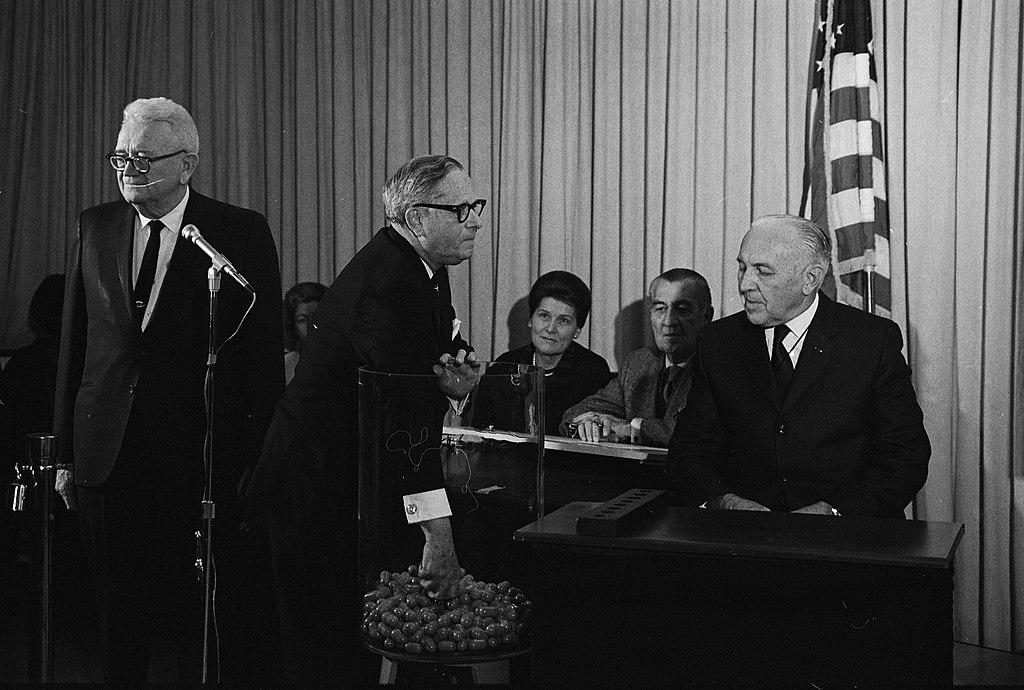
\includegraphics[width=0.8\linewidth,height=\textheight,keepaspectratio]{images/1969_draft_lottery_photo.jpg}

}

\caption{\label{fig-draft-lottery-photo}Congressman Alexander Pirnie
(R-NY) drawing the first capsule for the Selective Service draft, Dec 1,
1969. \emph{Source}: Wikipedia \url{https://bit.ly/45c23sB}}

\end{figure}%

In an attempt to make the selection process also transparent, the
proceeding was covered on radio, TV and film and the dates posted in
order on a large display board. The first capsule---drawn by Congressman
Alexander Pirnie (R-NY) of the House Armed Services
Committee---contained the date September 14, so all men born on
September 14 in any year between 1944 and 1950 were assigned lottery
number 1, and would be drafted first. April 24 was drawn next, then
December 30, February 14, and so on until June 8, selected last. At the
time of the drawing, US officials stated that those with birthdays drawn
in the first third would almost certainly be drafted, while those in the
last third would probably avoid the draft
(\citeproc{ref-Fienberg:71}{Fienberg, 1971}).

I watched this unfold with considerable interest because I was eligible
for the Draft that year. I was dismayed when my birthday, May 7, came up
ranked 35. \textbf{Ugh!} Could some data analysis and graphics get me
out of my funk?

The data, from the official
\href{https://www.sss.gov/wp-content/uploads/2020/03/1970-Vietnam-Lottery.pdf}{Selective
Service listing} are contained in the dataset
\texttt{vcdExtra::Draft1970} \index{Draft1970@\texttt{Draft1970} data}
\index{datasets!Draft1970@\texttt{Draft1970}}
\index{vcdExtra@\texttt{vcdExtra} package}
\index{packages!vcdExtra@\texttt{vcdExtra}}, ordered by \texttt{Month}
and birthdate (\texttt{Day}), with \texttt{Rank} as the order in which
the birthdates were drawn.

\begin{Shaded}
\begin{Highlighting}[]
\FunctionTok{library}\NormalTok{(ggplot2)}
\FunctionTok{library}\NormalTok{(dplyr)}
\FunctionTok{data}\NormalTok{(Draft1970, }\AttributeTok{package =} \StringTok{"vcdExtra"}\NormalTok{)}
\NormalTok{dplyr}\SpecialCharTok{::}\FunctionTok{glimpse}\NormalTok{(Draft1970)}
\CommentTok{\# Rows: 366}
\CommentTok{\# Columns: 3}
\CommentTok{\# $ Day   \textless{}int\textgreater{} 1, 2, 3, 4, 5, 6, 7, 8, 9, 10, 11, 12, 13, 14, 15, 1\textasciitilde{}}
\CommentTok{\# $ Rank  \textless{}int\textgreater{} 305, 159, 251, 215, 101, 224, 306, 199, 194, 325, 32\textasciitilde{}}
\CommentTok{\# $ Month \textless{}ord\textgreater{} Jan, Jan, Jan, Jan, Jan, Jan, Jan, Jan, Jan, Jan, Ja\textasciitilde{}}
\end{Highlighting}
\end{Shaded}

A basic scatterplot, slightly prettified, is shown in
Figure~\ref{fig-draft-gg1}. The points are colored by month, and month
labels are shown at the bottom.

\begin{Shaded}
\begin{Highlighting}[]
\CommentTok{\# make markers for months at their mid points}
\NormalTok{months }\OtherTok{\textless{}{-}} \FunctionTok{data.frame}\NormalTok{(}
  \AttributeTok{month =}\FunctionTok{unique}\NormalTok{(Draft1970}\SpecialCharTok{$}\NormalTok{Month),}
  \AttributeTok{mid =} \FunctionTok{seq}\NormalTok{(}\DecValTok{15}\NormalTok{, }\DecValTok{365{-}15}\NormalTok{, }\AttributeTok{by =} \DecValTok{30}\NormalTok{))}

\NormalTok{ggplot2}\SpecialCharTok{::} \FunctionTok{theme\_set}\NormalTok{(}\FunctionTok{theme\_bw}\NormalTok{(}\AttributeTok{base\_size =} \DecValTok{16}\NormalTok{))}
\NormalTok{gg }\OtherTok{\textless{}{-}} \FunctionTok{ggplot}\NormalTok{(Draft1970, }\FunctionTok{aes}\NormalTok{(}\AttributeTok{x =}\NormalTok{ Day, }\AttributeTok{y =}\NormalTok{ Rank)) }\SpecialCharTok{+}
  \FunctionTok{geom\_point}\NormalTok{(}\AttributeTok{size =} \FloatTok{2.5}\NormalTok{, }\AttributeTok{shape =} \DecValTok{21}\NormalTok{, }
             \AttributeTok{alpha =} \FloatTok{0.3}\NormalTok{, }
             \AttributeTok{color =} \StringTok{"black"}\NormalTok{, }
             \FunctionTok{aes}\NormalTok{(}\AttributeTok{fill=}\NormalTok{Month)}
\NormalTok{  ) }\SpecialCharTok{+}
  \FunctionTok{scale\_fill\_manual}\NormalTok{(}\AttributeTok{values =} \FunctionTok{rainbow}\NormalTok{(}\DecValTok{12}\NormalTok{)) }\SpecialCharTok{+}
  \FunctionTok{geom\_text}\NormalTok{(}\AttributeTok{data=}\NormalTok{months, }\FunctionTok{aes}\NormalTok{(}\AttributeTok{x=}\NormalTok{mid, }\AttributeTok{y=}\DecValTok{0}\NormalTok{, }\AttributeTok{label=}\NormalTok{month), }\AttributeTok{nudge\_x =} \DecValTok{5}\NormalTok{) }\SpecialCharTok{+}
  \FunctionTok{geom\_smooth}\NormalTok{(}\AttributeTok{method =} \StringTok{"lm"}\NormalTok{, }\AttributeTok{formula =}\NormalTok{ y }\SpecialCharTok{\textasciitilde{}} \DecValTok{1}\NormalTok{,}
              \AttributeTok{col =} \StringTok{"black"}\NormalTok{, }\AttributeTok{fill=}\StringTok{"grey"}\NormalTok{, }\AttributeTok{linetype =} \StringTok{"dashed"}\NormalTok{, }\AttributeTok{alpha=}\FloatTok{0.6}\NormalTok{) }\SpecialCharTok{+}
  \FunctionTok{labs}\NormalTok{(}\AttributeTok{x =} \StringTok{"Day of the year"}\NormalTok{,}
       \AttributeTok{y =} \StringTok{"Lottery rank"}\NormalTok{) }\SpecialCharTok{+}
  \FunctionTok{theme}\NormalTok{(}\AttributeTok{legend.position =} \StringTok{"none"}\NormalTok{) }
\NormalTok{gg}
\end{Highlighting}
\end{Shaded}

\begin{figure}[htb!]

\centering{

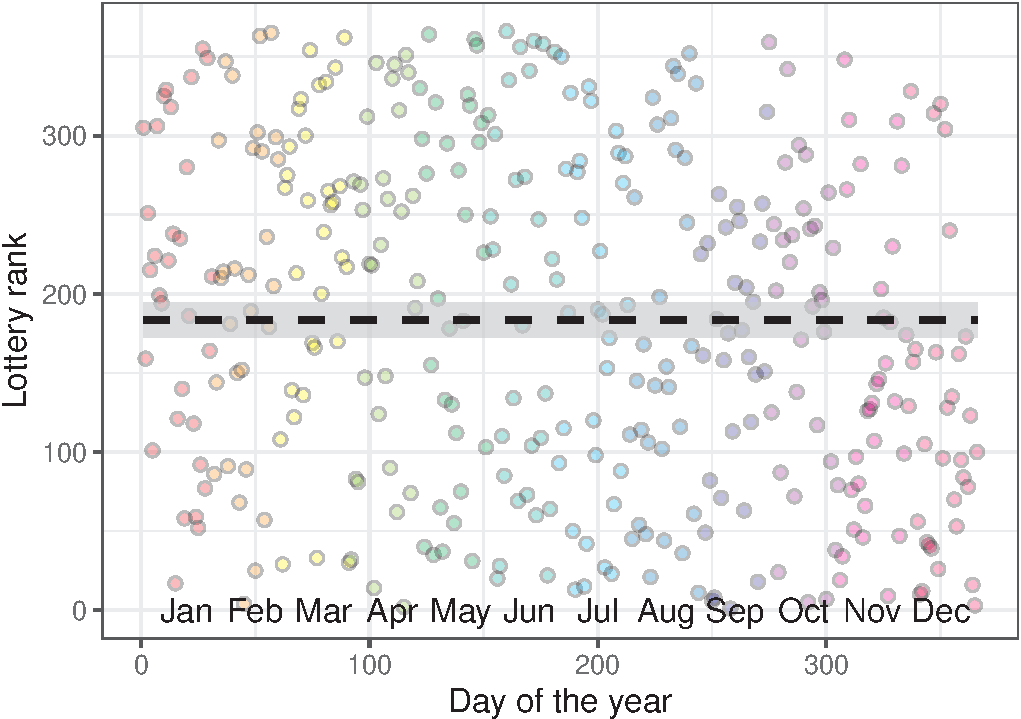
\includegraphics[width=0.8\linewidth,height=\textheight,keepaspectratio]{figs/ch03/fig-draft-gg1-1.pdf}

}

\caption{\label{fig-draft-gg1}Basic scatterplot of 1970 Draft Lottery
data plotting rank order of selection against birthdates in the year.
Points are colored by month. The horizontal line is at the average
rank.}

\end{figure}%

The ranks do seem to be essentially random. Is there any reason to
suspect a flaw in the selection process, as I firmly hoped at the time?

If you stare at the graph in Figure~\ref{fig-draft-gg1} long enough, you
just can make out a sparsity of points in the upper right corner and
also in the lower left corner compared to the opposite corners. But
probably not until I told you where to look.

\index{1970 draft lottery|)}

\subsubsection*{Visual smoothers}\label{visual-smoothers}
\addcontentsline{toc}{subsubsection}{Visual smoothers}

Fitting a linear regression line or a smoothed (loess) curve can bring
out the signal lurking in the background of a field of nearly random
points. Figure~\ref{fig-draft-gg2} shows a definite trend to lower ranks
for birthdays toward the end of the year. Those born earlier in the year
were more likely to be given lower ranks, calling them up sooner for the
draft. \index{loess} \index{smoother!loess}

\begin{Shaded}
\begin{Highlighting}[]
\FunctionTok{ggplot}\NormalTok{(Draft1970, }\FunctionTok{aes}\NormalTok{(}\AttributeTok{x =}\NormalTok{ Day, }\AttributeTok{y =}\NormalTok{ Rank)) }\SpecialCharTok{+}
  \FunctionTok{geom\_point}\NormalTok{(}\AttributeTok{size =} \FloatTok{2.5}\NormalTok{, }\AttributeTok{shape =} \DecValTok{21}\NormalTok{, }
             \AttributeTok{alpha =} \FloatTok{0.3}\NormalTok{, }
             \AttributeTok{color =} \StringTok{"black"}\NormalTok{, }
             \FunctionTok{aes}\NormalTok{(}\AttributeTok{fill=}\NormalTok{Month)) }\SpecialCharTok{+}
  \FunctionTok{scale\_fill\_manual}\NormalTok{(}\AttributeTok{values =} \FunctionTok{rainbow}\NormalTok{(}\DecValTok{12}\NormalTok{)) }\SpecialCharTok{+}
  \FunctionTok{geom\_smooth}\NormalTok{(}\AttributeTok{method =} \StringTok{"lm"}\NormalTok{, }\AttributeTok{formula =}\NormalTok{ y}\SpecialCharTok{\textasciitilde{}}\DecValTok{1}\NormalTok{,}
              \AttributeTok{se =} \ConstantTok{FALSE}\NormalTok{,}
              \AttributeTok{col =} \StringTok{"black"}\NormalTok{, }\AttributeTok{fill=}\StringTok{"grey"}\NormalTok{, }\AttributeTok{linetype =} \StringTok{"dashed"}\NormalTok{, }\AttributeTok{alpha=}\FloatTok{0.6}\NormalTok{) }\SpecialCharTok{+}
  \FunctionTok{geom\_smooth}\NormalTok{(}\AttributeTok{method =} \StringTok{"loess"}\NormalTok{, }\AttributeTok{formula =}\NormalTok{ y}\SpecialCharTok{\textasciitilde{}}\NormalTok{x,}
              \AttributeTok{color =} \StringTok{"blue"}\NormalTok{, }\AttributeTok{se =} \ConstantTok{FALSE}\NormalTok{,}
              \AttributeTok{alpha=}\FloatTok{0.25}\NormalTok{) }\SpecialCharTok{+}
  \FunctionTok{geom\_smooth}\NormalTok{(}\AttributeTok{method =} \StringTok{"lm"}\NormalTok{, }\AttributeTok{formula =}\NormalTok{ y}\SpecialCharTok{\textasciitilde{}}\NormalTok{x,}
              \AttributeTok{color =} \StringTok{"darkgreen"}\NormalTok{,}
              \AttributeTok{fill =} \StringTok{"darkgreen"}\NormalTok{, }
              \AttributeTok{alpha=}\FloatTok{0.25}\NormalTok{) }\SpecialCharTok{+}
  \FunctionTok{geom\_text}\NormalTok{(}\AttributeTok{data=}\NormalTok{months, }\FunctionTok{aes}\NormalTok{(}\AttributeTok{x=}\NormalTok{mid, }\AttributeTok{y=}\DecValTok{0}\NormalTok{, }\AttributeTok{label=}\NormalTok{month), }\AttributeTok{nudge\_x =} \DecValTok{5}\NormalTok{) }\SpecialCharTok{+}
  \FunctionTok{labs}\NormalTok{(}\AttributeTok{x =} \StringTok{"Day of the year"}\NormalTok{,}
       \AttributeTok{y =} \StringTok{"Lottery rank"}\NormalTok{) }\SpecialCharTok{+}
  \FunctionTok{theme}\NormalTok{(}\AttributeTok{legend.position =} \StringTok{"none"}\NormalTok{) }
\end{Highlighting}
\end{Shaded}

\begin{figure}[htb!]

\centering{

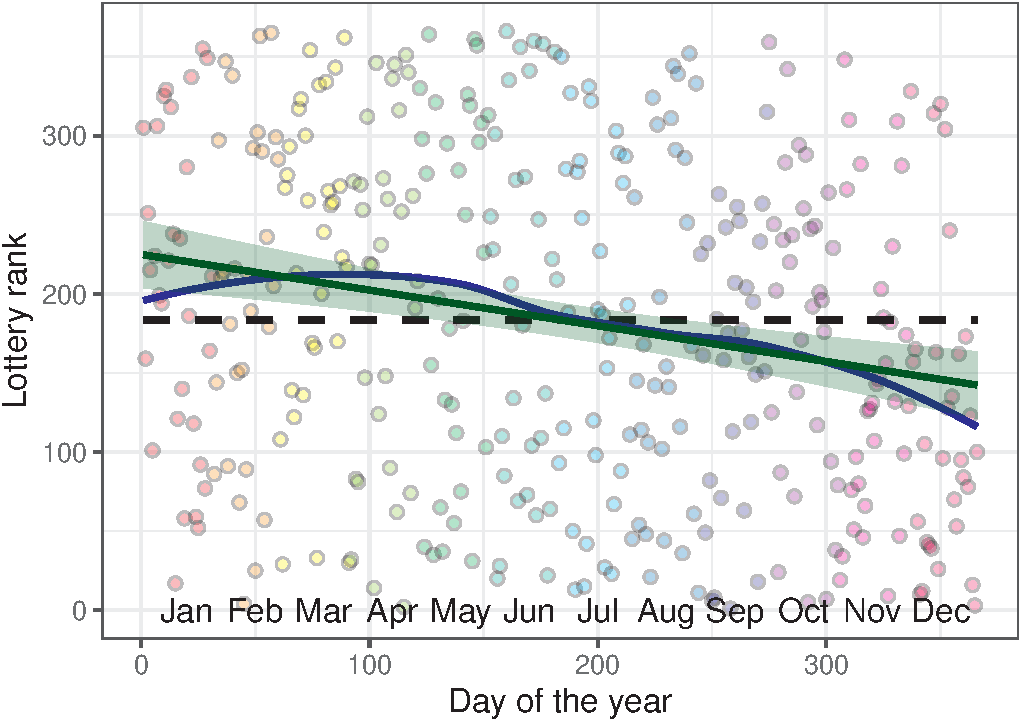
\includegraphics[width=0.8\linewidth,height=\textheight,keepaspectratio]{figs/ch03/fig-draft-gg2-1.pdf}

}

\caption{\label{fig-draft-gg2}Enhanced scatterplot of 1970 Draft Lottery
data adding a linear regression line and loess smooth.}

\end{figure}%

Is this a real effect? Even though the points seem to be random over the
year, linear regression of \texttt{Rank} on \texttt{Day} shows a highly
significant negative effect even though the correlation\footnote{Because
  both days of the year and rank in the lottery are the integers, 1 to
  366, the Pearson correlation and Spearman rank order correlation are
  identical.} is small (\(r = -0.226\)). The slope, -0.226, means that
for each additional day in the year the lottery rank decreases about 1/4
toward the front of the draft line; that's nearly 7 ranks per month.

\begin{Shaded}
\begin{Highlighting}[]
\NormalTok{draft.mod }\OtherTok{\textless{}{-}} \FunctionTok{lm}\NormalTok{(Rank }\SpecialCharTok{\textasciitilde{}}\NormalTok{ Day, }\AttributeTok{data=}\NormalTok{Draft1970)}
\FunctionTok{with}\NormalTok{(Draft1970, }\FunctionTok{cor}\NormalTok{(Day, Rank))}
\CommentTok{\# [1] {-}0.226}
\FunctionTok{coef}\NormalTok{(draft.mod)}
\CommentTok{\# (Intercept)         Day }
\CommentTok{\#     224.913      {-}0.226}
\end{Highlighting}
\end{Shaded}

So, smoothing the data, using either the linear regression line or a
nonparametric smoother is one important technique for seeing a weak
signal in a noisy background.

\subsubsection*{Visual summaries}\label{visual-summaries}
\addcontentsline{toc}{subsubsection}{Visual summaries}

Another way to enhance the signal-to-noise ratio of a graph is to plot
summaries of the messy data points. For example, you might make boxplots
of the ranks by month, or calculate and plot the mean or median rank by
month and plot those together with some indication of variability within
month.

Figure~\ref{fig-draft-means} plots the average \texttt{Rank} for each
month with error bars showing the mean \(\pm 1\) standard errors against
the average \texttt{Day}. The message of rank decreasing nearly linearly
with month is now more dramatic, partly because I decreased the range of
the y-axis.\footnote{Restricting the y-axis range in plots can sometimes
  be a graphical sin. It can distort the visual representation of the
  data, making differences appear larger than they actually are, and
  potentially misleading the viewer. But this is not a sin, when it
  serves a communication goal, which in Figure~\ref{fig-draft-means} is
  to focus attention on the relative changes in lottery rank over the
  year. Using a visual cue like a broken axis in the axis is one way to
  avoid misinterpretation. For \texttt{ggplot} graphs, the
  \textcolor{brown}{\texttt{\textbf{ggbreak}}} package %
     \index{ggbreak@\texttt{ggbreak} package}%
     \index{packages!ggbreak@\texttt{ggbreak}}%
       is useful for this purpose.} The correlation between the means is
\(r = -0.867\); the slope is -0.231, similar to what we found for the
raw data.

\begin{Shaded}
\begin{Highlighting}[]
\NormalTok{means }\OtherTok{\textless{}{-}}\NormalTok{ Draft1970 }\SpecialCharTok{|\textgreater{}}
  \FunctionTok{group\_by}\NormalTok{(Month) }\SpecialCharTok{|\textgreater{}}
  \FunctionTok{summarize}\NormalTok{(}\AttributeTok{Day =} \FunctionTok{mean}\NormalTok{(Day),}
            \AttributeTok{se =} \FunctionTok{sd}\NormalTok{(Rank}\SpecialCharTok{/} \FunctionTok{sqrt}\NormalTok{(}\FunctionTok{n}\NormalTok{())),}
            \AttributeTok{Rank =} \FunctionTok{mean}\NormalTok{(Rank)) }

\FunctionTok{ggplot}\NormalTok{(}\FunctionTok{aes}\NormalTok{(}\AttributeTok{x =}\NormalTok{ Day, }\AttributeTok{y =}\NormalTok{ Rank), }\AttributeTok{data=}\NormalTok{means) }\SpecialCharTok{+}
  \FunctionTok{geom\_point}\NormalTok{(}\AttributeTok{size =} \DecValTok{4}\NormalTok{) }\SpecialCharTok{+}
  \FunctionTok{geom\_smooth}\NormalTok{(}\AttributeTok{method =} \StringTok{"lm"}\NormalTok{, }\AttributeTok{formula =}\NormalTok{ y}\SpecialCharTok{\textasciitilde{}}\NormalTok{x,}
              \AttributeTok{color =} \StringTok{"blue"}\NormalTok{, }\AttributeTok{fill =} \StringTok{"blue"}\NormalTok{, }\AttributeTok{alpha =} \FloatTok{0.1}\NormalTok{) }\SpecialCharTok{+}
  \FunctionTok{geom\_errorbar}\NormalTok{(}\FunctionTok{aes}\NormalTok{(}\AttributeTok{ymin =}\NormalTok{ Rank}\SpecialCharTok{{-}}\NormalTok{se, }\AttributeTok{ymax =}\NormalTok{ Rank}\SpecialCharTok{+}\NormalTok{se), }
                \AttributeTok{width =} \DecValTok{8}\NormalTok{, }\AttributeTok{linewidth =} \FloatTok{1.3}\NormalTok{) }\SpecialCharTok{+}
  \FunctionTok{geom\_text}\NormalTok{(}\AttributeTok{data=}\NormalTok{months, }\FunctionTok{aes}\NormalTok{(}\AttributeTok{x=}\NormalTok{mid, }\AttributeTok{y=}\DecValTok{100}\NormalTok{, }\AttributeTok{label=}\NormalTok{month), }\AttributeTok{nudge\_x =} \DecValTok{5}\NormalTok{) }\SpecialCharTok{+}
  \FunctionTok{ylim}\NormalTok{(}\DecValTok{100}\NormalTok{, }\DecValTok{250}\NormalTok{) }\SpecialCharTok{+}
  \FunctionTok{labs}\NormalTok{(}\AttributeTok{x =} \StringTok{"Average day of the year"}\NormalTok{,}
       \AttributeTok{y =} \StringTok{"Average lottery rank"}\NormalTok{)}
\end{Highlighting}
\end{Shaded}

\begin{figure}[htb!]

\centering{

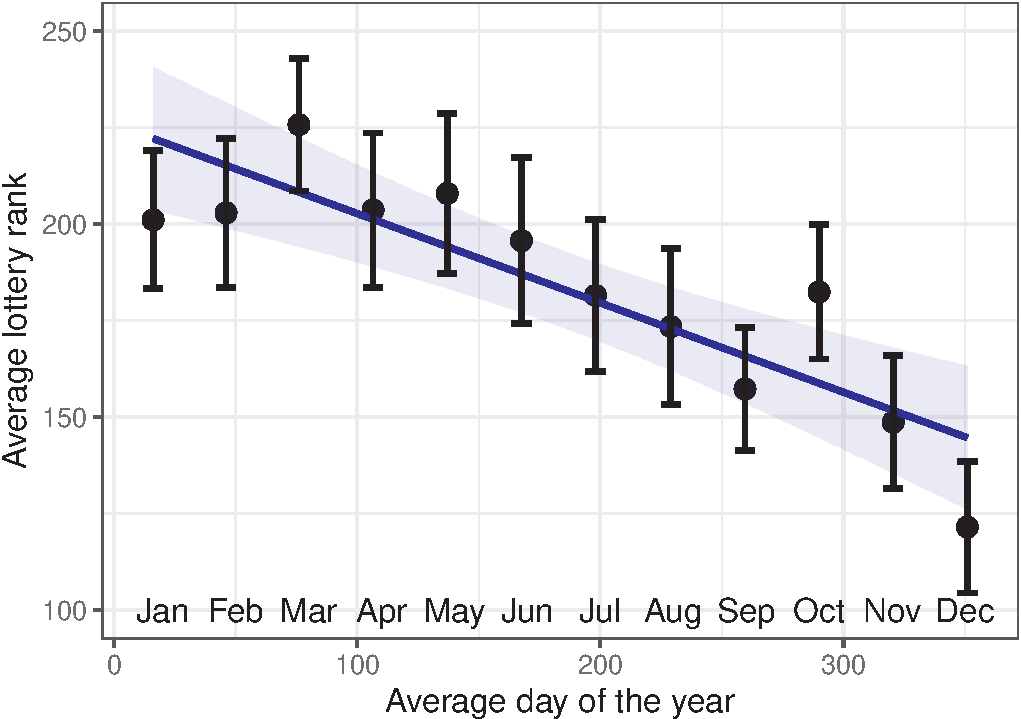
\includegraphics[width=0.8\linewidth,height=\textheight,keepaspectratio]{figs/ch03/fig-draft-means-1.pdf}

}

\caption{\label{fig-draft-means}Plot of the average rank per month with
\(\pm 1\) standard error bars. The line shows the least squares
regression line, treating months as equally spaced. The vertical axis
has been truncated to highlight the decrease in lottery rank over the
year.}

\end{figure}%

The visual impression of a linearly decreasing trend in lottery rank is
much stronger in Figure~\ref{fig-draft-means} than in
Figure~\ref{fig-draft-gg2} for two reasons:

\begin{itemize}
\tightlist
\item
  Replacing the data points with their means strengthens the signal in
  relation to noise, which is essentially eliminated by plotting means
  and error bars rather than the raw data. This is an example of
  \emph{visual thinning} (Section~\ref{sec-visual-thinning}), reducing
  visual complexity to highlight an overall pattern.
\item
  The narrower vertical range (100--250) in the plot of means makes the
  slope of the line appear steeper. (However, the slope of the means,
  \(b = -0.231\) is nearly the same as that for the data points.) The
  narrower range also makes deviations from the regression line more
  noticeable.
\end{itemize}

\subsubsection*{What happened here?}\label{what-happened-here}
\addcontentsline{toc}{subsubsection}{What happened here?}

Previous lotteries carried out by drawing capsules from a container had
occasionally suffered the embarrassment that an empty capsule was
selected because of vigorous mixing
(\citeproc{ref-Fienberg:71}{Fienberg, 1971}). So for the 1970 lottery,
the birthdate capsules were put in cardboard boxes, one for each month
and these were carefully emptied into the glass container in order of
month: Jan., Feb., through Dec., and gently shaken in atop the pile
already there.

All might have been well had the persons drawing the capsules put their
hand in truly randomly, but generally they picked from toward the top of
the container. Consequently, those born later in the year had a greater
chance of being picked earlier.

There was considerable criticism of this procedure once the flaw had
been revealed by analyses such as described here. In the following year,
the Selective Service called upon the National Bureau of Standards to
devise a better procedure. In 1971 they used two drums, one with the
dates of the year and another with the rank numbers 1-366. As a date
capsule was drawn randomly from the first drum, another from the numbers
drum was picked simultaneously, giving a doubly-randomized sequence.

Of course, if they had R, the entire process could have been done using
\texttt{sample()} \ixfunc{sample()} :

\begin{Shaded}
\begin{Highlighting}[]
\FunctionTok{set.seed}\NormalTok{(}\DecValTok{42}\NormalTok{)}
\NormalTok{date }\OtherTok{=} \FunctionTok{seq}\NormalTok{(}\FunctionTok{as.Date}\NormalTok{(}\StringTok{"1971{-}01{-}01"}\NormalTok{), }
           \FunctionTok{as.Date}\NormalTok{(}\StringTok{"1971{-}12{-}31"}\NormalTok{), }\AttributeTok{by=}\StringTok{"+1 day"}\NormalTok{)}
\NormalTok{rank }\OtherTok{=} \FunctionTok{sample}\NormalTok{(}\FunctionTok{seq\_along}\NormalTok{(date))}
\NormalTok{draft1971 }\OtherTok{\textless{}{-}} \FunctionTok{data.frame}\NormalTok{(date, rank)}

\FunctionTok{head}\NormalTok{(draft1971, }\DecValTok{3}\NormalTok{)}
\CommentTok{\#         date rank}
\CommentTok{\# 1 1971{-}01{-}01   49}
\CommentTok{\# 2 1971{-}01{-}02  321}
\CommentTok{\# 3 1971{-}01{-}03  153}
\FunctionTok{tail}\NormalTok{(draft1971, }\DecValTok{3}\NormalTok{)}
\CommentTok{\#           date rank}
\CommentTok{\# 363 1971{-}12{-}29    8}
\CommentTok{\# 364 1971{-}12{-}30  333}
\CommentTok{\# 365 1971{-}12{-}31  132}
\end{Highlighting}
\end{Shaded}

And, what would have happened to me and all others born on a May 7th, if
they did it this way? My lottery rank would have 274!\footnote{A
  personal note: I escaped being drafted, but I moved to Canada in 1971.
  Looking back today, it's one of the best decisions I ever made.}

\begin{Shaded}
\begin{Highlighting}[]
\NormalTok{me }\OtherTok{\textless{}{-}} \FunctionTok{as.Date}\NormalTok{(}\StringTok{"1971{-}05{-}07"}\NormalTok{)}
\NormalTok{draft1971[draft1971}\SpecialCharTok{$}\NormalTok{date }\SpecialCharTok{==}\NormalTok{ me,]}
\CommentTok{\#           date rank}
\CommentTok{\# 127 1971{-}05{-}07  274}
\end{Highlighting}
\end{Shaded}

\section{Plots for data analysis}\label{sec-plots-data-analysis}

Visualization methods take an enormous variety of forms, so it is useful
to distinguish several broad categories according to their \emph{use in
data analysis}:

\begin{itemize}
\item
  \textbf{data plots}: primarily plot the raw data, often with
  annotations to aid interpretation. 1D plots include boxplots, violin
  plots and dot plots, sometimes in combination; univariate
  distributions can also be portrayed in histograms and density
  estimates. 2D plots are most often scatterplots, favorably enhanced
  using regression lines and smooths, data ellipses, rug plots and
  marginal distributions. A survey of these methods is presented in
  Section~\ref{sec-bivariate_summaries}. \index{data plots}
\item
  \textbf{reconnaissance plots}: with more than a few variables,
  reconnaissance plots provide a high-level, bird's-eye overview of the
  data, allowing you to see patterns that might not be visible in a set
  of separate plots. Some examples are scatterplot matrices
  (Section~\ref{sec-scatmat}) showing all bivariate plots of variables
  in a dataset; correlation diagrams (Section~\ref{sec-corrgram}), using
  visual glyphs to represent the correlations between all pairs of
  variables and ``trellis'' or faceted plots that show how a focal
  relation of one or more variables differs across values of other
  variables. \index{reconnaissance plots}
\item
  \textbf{model plots}: plot the results of a fitted model, such as a
  regression line or curve to show uncertainty, or a regression surface
  in 3D, or a plot of coefficients in model together with confidence
  intervals. Figure~\ref{fig-draft-means} is a simple example.
  \index{uncertainty}
\end{itemize}

Other model plots try to take into account that a fitted model may
involve more variables than can be shown in a static 2D plot. Some
examples of these are \emph{added variable plots}
(Section~\ref{sec-avplots}), and \emph{marginal effect plots}
(Section~\ref{sec-effect-displays}), both of which attempt to show the
\emph{net} relation of two focal variables, controlling or adjusting for
other variables in a model. \index{model plots}
\index{added-variable plots} \index{effect plots}

\begin{itemize}
\item
  \textbf{diagnostic plots}: indicating potential problems with the
  fitted model. For linear models, these include residual plots,
  influence plots, plots for testing homogeneity of variance and so
  forth, illustrated in Section~\ref{sec-diagnostic-plots}. Plots for
  diagnosing problems with multivariate models are discussed in
  Section~\ref{sec-model-diagnostics-MLM}. \index{diagnostic plots}
\item
  \textbf{dimension reduction plots} : plot representations of the data
  in a space of fewer dimensions than the number of variables in the
  analysis. Simple examples include principal components analysis (PCA)
  and the related biplots, and multidimensional scaling (MDS) methods.
  This is the topic of Chapter~\ref{sec-pca-biplot}, but this powerful
  idea runs through the rest of the book. I refer to such plots as
  \emph{multivariate juicers}, because they can squeeze the essence of
  your data into low-D package, enhancing the flavor.
\end{itemize}

\subsection{Diagnostic plots}\label{diagnostic-plots}

Having fit a model, your next step should usually be to try to criticize
it by checking whether the assumptions of the model are met in your
data.

For example, the plot of the Davis data in Figure~\ref{fig-davis-reg1}
effectively fits a separate regression line for males and females, which
is expressed by the model formula
\texttt{repwt\ \textasciitilde{}\ weight\ *\ sex}. Having fit the model
using \texttt{lm()} \ixfunc{lm()} , the plot method for a \texttt{"lm"}
object produces a set of four diagnostic plots (called the ``regression
quartet'' Section~\ref{sec-regression-quartet}) designed to highlight
problems with the fitted model.

\begin{Shaded}
\begin{Highlighting}[]
\NormalTok{davis.mod }\OtherTok{\textless{}{-}} \FunctionTok{lm}\NormalTok{(repwt }\SpecialCharTok{\textasciitilde{}}\NormalTok{ weight }\SpecialCharTok{*}\NormalTok{ sex, }\AttributeTok{data=}\NormalTok{Davis)  }
\FunctionTok{plot}\NormalTok{(davis.mod, }
     \AttributeTok{cex.lab =} \FloatTok{1.2}\NormalTok{, }\AttributeTok{cex =} \FloatTok{1.1}\NormalTok{, }
     \AttributeTok{id.n =} \DecValTok{2}\NormalTok{, }\AttributeTok{cex.id =} \FloatTok{1.2}\NormalTok{, }\AttributeTok{lwd =} \DecValTok{2}\NormalTok{)}
\end{Highlighting}
\end{Shaded}

\begin{figure}[htb!]

\centering{

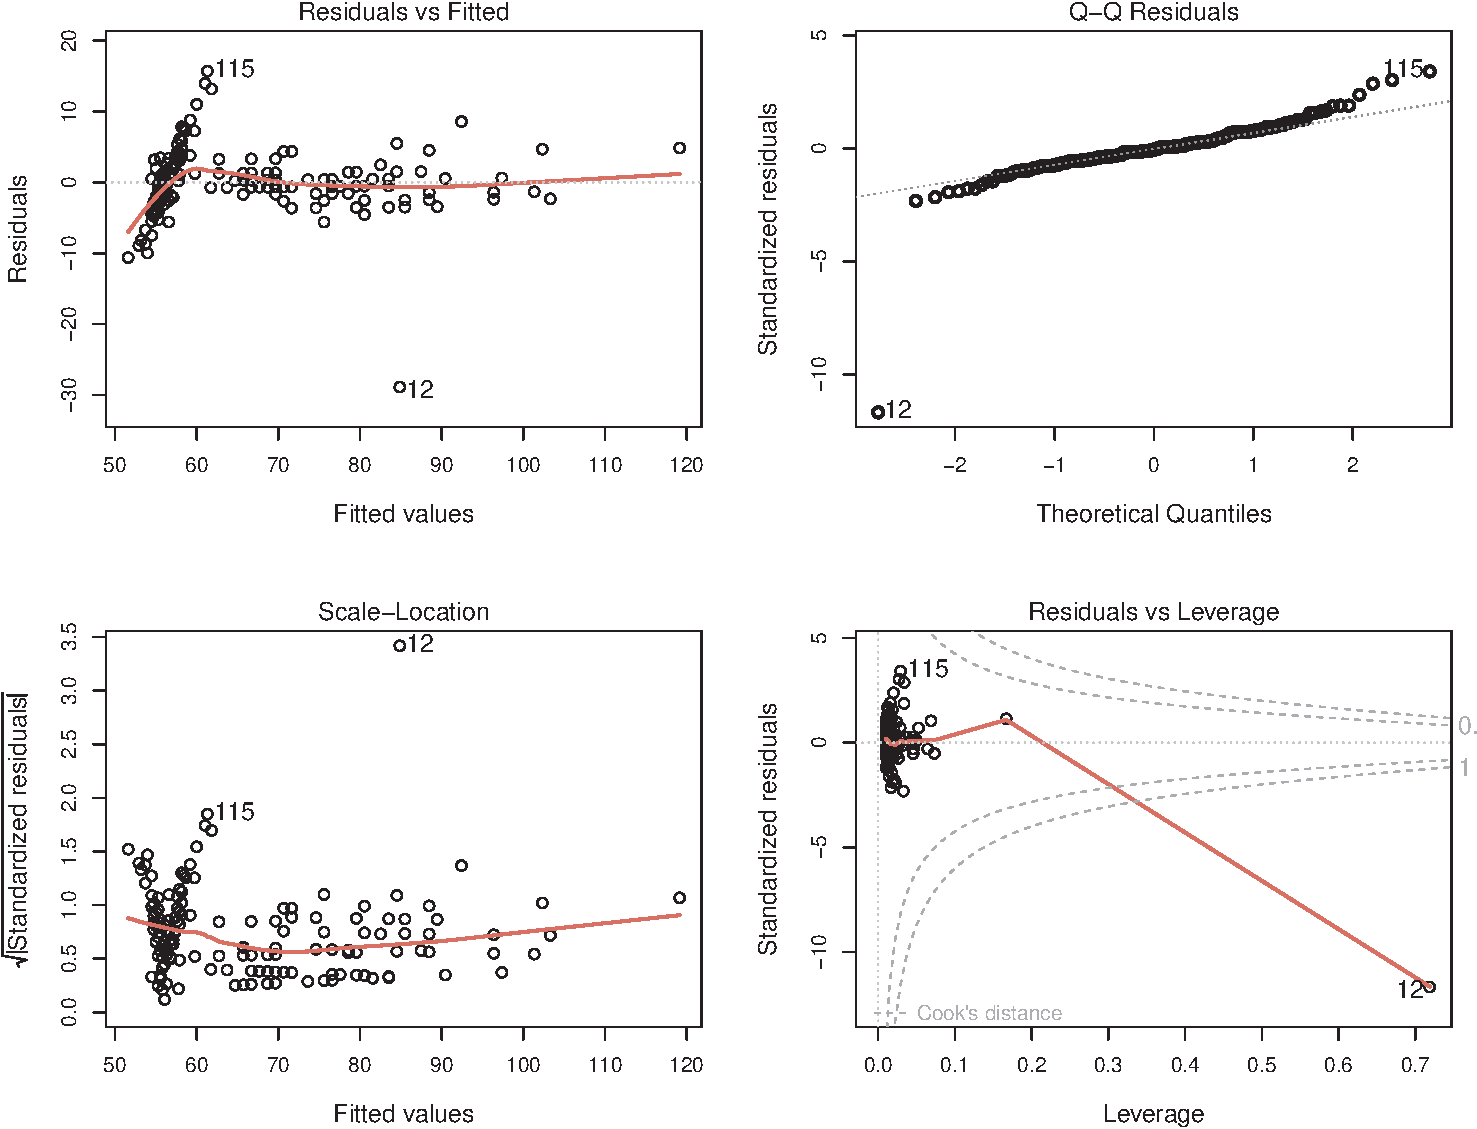
\includegraphics[width=0.9\linewidth,height=\textheight,keepaspectratio]{figs/ch03/fig-davis-diagnostic-1.pdf}

}

\caption{\label{fig-davis-diagnostic}Regression quartet: Four diagnostic
plots for the linear model fit to the Davis data. The details of these
plots are discussed in Section~\ref{sec-regression-quartet}.}

\end{figure}%

The details of such plots are discussed and illustrated in
Section~\ref{sec-regression-quartet}, so I will just point out one
useful feature here: that of point identification: the \texttt{id.n}
argument controls the number of most-extreme points to be labeled in
each panel. The point for the erroneous case 12 female who mis-recorded
her height as her weight sticks out a mile in all four panels.

\section{Principles of graphical
display}\label{principles-of-graphical-display}

\textbf{TODO}: This could be a separate chapter, supplementary materials
or excluded here

\begin{itemize}
\tightlist
\item
  Criteria for assessing graphs: communication goals
\item
  Effective data display:

  \begin{itemize}
  \tightlist
  \item
    Make the data stand out
  \item
    Make graphical comparison easy
  \item
    Effect ordering: For variables and unordered factors, arrange them
    according to the effects to be seen
  \end{itemize}
\item
  Visual thinning: As the data becomes more complex, focus more on
  impactful summaries
\end{itemize}

\section{What have we learned?}\label{what-have-we-learned}

This chapter demonstrates why visualization isn't just a
``nice-to-have'' feature in data analysis-----it's absolutely essential.
Through compelling historical examples and modern techniques, we've
discovered some fundamental idea that every data analyst should embrace:

\begin{itemize}
\item
  \textbf{Summary statistics can conceal the truth}: Anscombe's Quartet
  reveals that datasets can have identical means, correlations, and
  regression coefficients yet tell completely different stories. The
  quartet's four plots-----pure error, lack of fit, outliers, and
  influence-----show that numerical summaries without visualization can
  lead us wildly astray. Modern extensions like the Datasaurus Dozen
  prove this isn't just a quirky historical example-----you can
  literally hide a dinosaur in your data while maintaining identical
  statistical properties! Talk about the dinosaur in the room!
\item
  \textbf{One rogue data point can hijack your entire analysis}:
  Plotting the raw data facilitates critical engagement with our
  statistical models. The Davis weight study demonstrates how a single
  influential observation (one participant who accidentally switched
  their reported and measured weights) can completely distort
  relationships between variables. What appeared to be a puzzling gender
  difference in the reliability of self-reported weight vanished once
  the data was plotted and the outlier revealed itself as a simple
  recording error.
\item
  \textbf{Meaning becomes more apparent through thoughtful
  visualizations of well-considered models}: Statistical modeling helps
  guide your attention in what might otherwise be a chaotic plot of raw
  data. The 1970 Draft Lottery story shows how graphics can reveal
  systematic bias hiding in apparently random data. While individual
  lottery numbers seemed random, smoothing techniques and summary plots
  exposed a clear pattern-----later birthdays were systematically
  favored due to poor mixing of the lottery capsules. Sometimes the most
  important patterns are the ones that whisper rather than shout.
\item
  \textbf{Different plot types serve different purposes}: The chapter
  introduces a taxonomy of visualization goals that helps us choose the
  right tool for each analytical task. Data plots show raw observations,
  reconnaissance plots provide bird's-eye overviews of complex datasets,
  model plots reveal fitted relationships, diagnostic plots expose model
  problems, and dimension reduction plots tame high-dimensional
  complexity. Each serves a distinct role in the analytical process.
\item
  \textbf{Visual enhancement amplifies signal over noise}: Whether
  through smoothing lines, statistical summaries, or careful use of
  color and annotation, the chapter shows how thoughtful visual design
  can make weak patterns stand out dramatically. The Draft Lottery
  analysis becomes far more convincing when we plot monthly averages
  rather than individual data points, transforming a subtle correlation
  into an unmistakable trend.
\end{itemize}

The overarching message is clear: in an era where we can compute any
statistic imaginable, the not-so-humble graph remains our most powerful
tool for understanding what our data are really trying to tell us. As
the Farquhar brothers noted over a century ago, getting information from
tables alone is like extracting sunlight from a cucumber---possible in
theory, but why make it so hard on yourself?

\part{Exploratory Methods}

\chapter{Plots of Multivariate Data}\label{sec-multivariate_plots}

\begin{quote}
\emph{There is no excuse for failing to plot and look.} \emph{The
greatest value of a picture is when it forces us to notice what we never
expected to see.} --- John W. Tukey (\citeproc{ref-Tukey:77}{1977}),
\emph{Exploratory Data Analysis} \index{Tukey, John}
\end{quote}

These quotes from John Tukey remind us that data analysis should nearly
always start with graphs to help us understand the main features of our
data. It is important to understand the general \emph{patterns} and
\emph{trends}: Are relationships increasing or decreasing? Are they
approximately linear or non-linear? But it is also important to spot
\emph{anomalies}: ``unusual'' observations, groups of points that seem
to differ from the rest, and so forth. As we saw with Anscombe's quartet
(Section~\ref{sec-anscombe}) and the Davis weight data
(Section~\ref{sec-davis}) numerical summaries hide features that are
immediately apparent in a plot. \index{quartet!Anscombe}

This chapter introduces a toolbox of basic graphical methods for
visualizing multivariate datasets. It starts with some simple techniques
to enhance the basic scatterplot with graphical \emph{annotations} such
as fitted lines, curves (Section~\ref{sec-bivariate_summaries}) and data
ellipses (Section~\ref{sec-data-ellipse}) which serve to add
\emph{visual summaries} of the relation between two variables.

To visualize more than two variables, we can view all pairs of variables
in a scatterplot matrix (Section~\ref{sec-scatmat}) or shift gears
entirely to show multiple variables along a set of parallel axes
(Section~\ref{sec-parcoord}).

As the number of variables increases, we may need to suppress details
with stronger summaries (Section~\ref{sec-visual-thinning}) for a
high-level reconnaissance of our data terrain, as we do by zooming out
on a map. For example, we can simply remove the data points or make them
nearly transparent to focus on the visual summaries provided by fitted
lines or other graphical summaries. \index{scatterplot matrix}

Another approach to visualizing high-D data uses \emph{animated tours}
(Section~\ref{sec-animated-tours}) to show the data in a sequence of
low-D projections, typically 2D, designed to reveal interesting features
that might not otherwise be visible. At a higher level of abstraction,
\emph{network diagrams} (Section~\ref{sec-network}) representing the
structure of correlations among a possibly large set of variables offer
another useful technique.

\textbf{Packages}

In this chapter I use the following packages. Load them now:

\begin{Shaded}
\begin{Highlighting}[]
\FunctionTok{library}\NormalTok{(car)}
\FunctionTok{library}\NormalTok{(ggplot2)}
\FunctionTok{library}\NormalTok{(dplyr)}
\FunctionTok{library}\NormalTok{(tidyr)}
\FunctionTok{library}\NormalTok{(corrplot)}
\FunctionTok{library}\NormalTok{(corrgram)}
\FunctionTok{library}\NormalTok{(GGally)}
\FunctionTok{library}\NormalTok{(ggdensity)}
\FunctionTok{library}\NormalTok{(patchwork)}
\FunctionTok{library}\NormalTok{(ggpcp)}
\FunctionTok{library}\NormalTok{(tourr)}
\FunctionTok{library}\NormalTok{(heplots)}
\FunctionTok{library}\NormalTok{(gggda)}

\CommentTok{\# set basic ggplot theme}
\NormalTok{ggplot2}\SpecialCharTok{::}\FunctionTok{theme\_set}\NormalTok{(}\FunctionTok{theme\_bw}\NormalTok{(}\AttributeTok{base\_size =} \DecValTok{14}\NormalTok{))}
\end{Highlighting}
\end{Shaded}

\section{Bivariate summaries}\label{sec-bivariate_summaries}

The basic scatterplot is the workhorse of multivariate data
visualization, showing how one variable, \(y\), often an outcome to be
explained by or varies with another, \(x\). It is a building block for
many useful techniques, so it is helpful to understand how it can be
used as a tool for thinking in a wider, multivariate context.

The essential idea is that we can start with a simple version of the
scatterplot and add annotations to show interesting features more
clearly. I consider the following here:

\begin{itemize}
\tightlist
\item
  \textbf{Smoothers}: Showing overall trends, perhaps in several forms,
  as visual summaries such as fitted regression lines or curves and
  nonparametric smoothers.
\item
  \textbf{Stratifiers}: Using color, shape or other features to identify
  subgroups; more generally, \emph{conditioning} on other variables in
  multi-panel displays;
\item
  \textbf{Data ellipses}: A compact 2D visual summary of bivariate
  linear relations and uncertainty assuming normality; more generally,
  contour plots of bivariate density. \index{smoother}
  \index{data ellipse} \index{stratifier} \index{uncertainty}
\end{itemize}

\begin{example}[]\protect\hypertarget{exm-salaries1}{}\label{exm-salaries1}

\textbf{Academic salaries}

Let's start with data on the academic salaries of faculty members
collected at a U.S. college for the purpose of assessing salary
differences between male and female faculty members, and perhaps address
anomalies in compensation. The dataset \texttt{carData::Salaries}
\index{Salaries@\texttt{Salaries} data}
\index{datasets!Salaries@\texttt{Salaries}}
\index{carData@\texttt{carData} package}
\index{packages!carData@\texttt{carData}} gives data on nine-month
salaries and other variables for 397 faculty members in the 2008-2009
academic year.

\begin{Shaded}
\begin{Highlighting}[]
\FunctionTok{data}\NormalTok{(Salaries, }\AttributeTok{package =} \StringTok{"carData"}\NormalTok{)}
\FunctionTok{str}\NormalTok{(Salaries)}
\CommentTok{\# \textquotesingle{}data.frame\textquotesingle{}: 397 obs. of  6 variables:}
\CommentTok{\#  $ rank         : Factor w/ 3 levels "AsstProf","AssocProf",..: 3 3 1 3 3 2 3 3 3 3 ...}
\CommentTok{\#  $ discipline   : Factor w/ 2 levels "A","B": 2 2 2 2 2 2 2 2 2 2 ...}
\CommentTok{\#  $ yrs.since.phd: int  19 20 4 45 40 6 30 45 21 18 ...}
\CommentTok{\#  $ yrs.service  : int  18 16 3 39 41 6 23 45 20 18 ...}
\CommentTok{\#  $ sex          : Factor w/ 2 levels "Female","Male": 2 2 2 2 2 2 2 2 2 1 ...}
\CommentTok{\#  $ salary       : int  139750 173200 79750 115000 141500 97000 175000 147765 119250 129000 ...}
\end{Highlighting}
\end{Shaded}

The most obvious, but perhaps naive, predictor of \texttt{salary} is
\texttt{years.since.phd}. For simplicity, I'll refer to this as years of
``experience.'' Before looking at differences between males and females,
we would want consider faculty \texttt{rank} (related also to
\texttt{yrs.service}) and \texttt{discipline}, recorded here as
\texttt{"A"} (``theoretical'' departments) or \texttt{"B"} (``applied''
departments). But, for a basic plot, we will ignore these for now to
focus on what can be learned from plot annotations.

\begin{Shaded}
\begin{Highlighting}[]
\NormalTok{gg1 }\OtherTok{\textless{}{-}} \FunctionTok{ggplot}\NormalTok{(Salaries, }
       \FunctionTok{aes}\NormalTok{(}\AttributeTok{x =}\NormalTok{ yrs.since.phd, }\AttributeTok{y =}\NormalTok{ salary)) }\SpecialCharTok{+}
  \FunctionTok{geom\_jitter}\NormalTok{(}\AttributeTok{size =} \DecValTok{2}\NormalTok{) }\SpecialCharTok{+}
  \FunctionTok{scale\_y\_continuous}\NormalTok{(}\AttributeTok{labels =}\NormalTok{ scales}\SpecialCharTok{::}\FunctionTok{dollar\_format}\NormalTok{(}
    \AttributeTok{prefix=}\StringTok{"$"}\NormalTok{, }\AttributeTok{scale =} \FloatTok{0.001}\NormalTok{, }\AttributeTok{suffix =} \StringTok{"K"}\NormalTok{)) }\SpecialCharTok{+}
  \FunctionTok{labs}\NormalTok{(}\AttributeTok{x =} \StringTok{"Years since PhD"}\NormalTok{,}
       \AttributeTok{y =} \StringTok{"Salary"}\NormalTok{) }

\NormalTok{gg1 }\SpecialCharTok{+} \FunctionTok{geom\_rug}\NormalTok{(}\AttributeTok{position =} \StringTok{"jitter"}\NormalTok{, }\AttributeTok{alpha =} \DecValTok{1}\SpecialCharTok{/}\DecValTok{4}\NormalTok{)}
\end{Highlighting}
\end{Shaded}

\begin{figure}[htb!]

\centering{

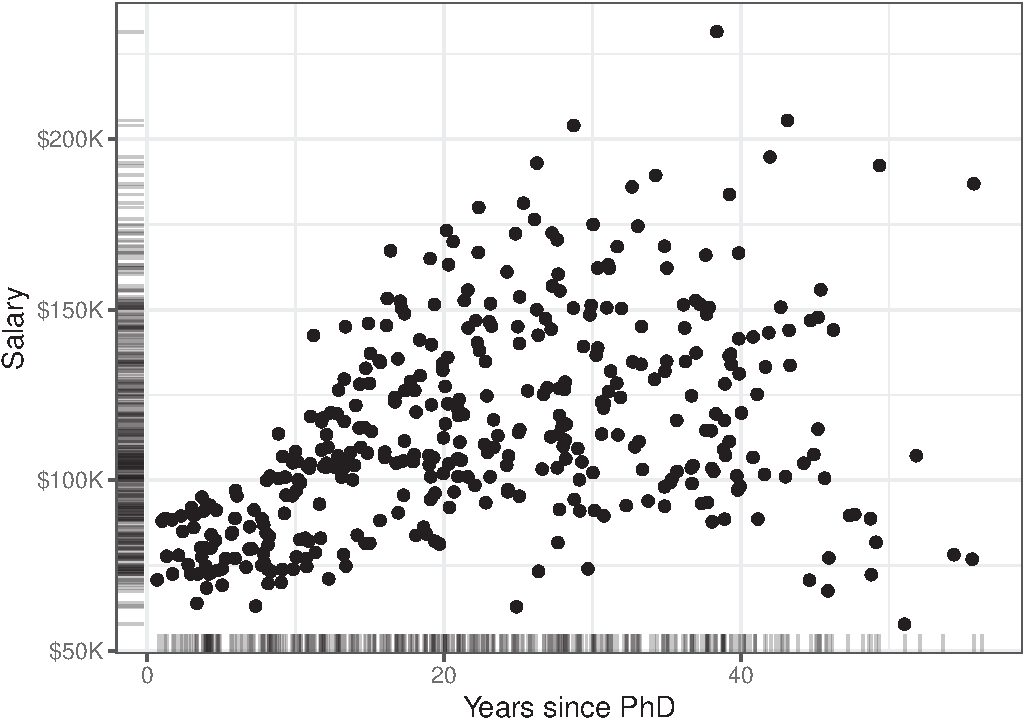
\includegraphics[width=0.8\linewidth,height=\textheight,keepaspectratio]{figs/ch04/fig-Salaries-scat-1.pdf}

}

\caption{\label{fig-Salaries-scat}Naive scatterplot of Salary vs.~years
since PhD, ignoring other variables, and without graphical annotations.}

\end{figure}%

There is quite a lot we can see ``just by looking'' at this simple plot,
but the main things are:

\begin{itemize}
\tightlist
\item
  Salary increases generally from 0 - 40 years since the PhD, but then
  maybe begins to drop off (partial retirement?);
\item
  Variability in salary increases among those with the same experience,
  a ``fan-shaped'' pattern that signals a violation of homogeneity of
  variance in simple regression;
\item
  Data beyond 50 years is thin, but there are some quite low salaries
  there. Adding rug plots to the X and Y axes is a simple but effective
  way to show the marginal distributions of the observations. Jitter and
  transparency helps to avoid overplotting due to discrete values.
\end{itemize}

\end{example}

\subsection{Smoothers}\label{smoothers}

\index{smoother|(}

Smoothers are among the most useful graphical annotations you can add to
such plots, giving a visual summary of how \(y\) changes with \(x\). The
most common smoother is a line showing the linear regression for \(y\)
given \(x\), expressed in math notation as
\(\mathbb{E} (y | x) = b_0 + b_1 x\). If there is doubt that a linear
relation is an adequate summary, you can try a quadratic or other
polynomial smoothers.

In \textcolor{brown}{\texttt{\textbf{ggplot2}}} %
   \index{ggplot2@\texttt{ggplot2} package}%
   \index{packages!ggplot2@\texttt{ggplot2}}%
     , these are easily added to a plot using \texttt{geom\_smooth()}
with \texttt{method\ =\ "lm"}, and a model \texttt{formula}, which (by
default) is \texttt{y\ \textasciitilde{}\ x} for a linear relation or
\texttt{y\ \textasciitilde{}\ poly(x,\ k)} for a polynomial of degree
\(k\).

\begin{Shaded}
\begin{Highlighting}[]
\NormalTok{gg1 }\SpecialCharTok{+} 
  \FunctionTok{geom\_smooth}\NormalTok{(}\AttributeTok{method =} \StringTok{"lm"}\NormalTok{, }\AttributeTok{formula =} \StringTok{"y \textasciitilde{} x"}\NormalTok{, }
              \AttributeTok{color =} \StringTok{"red"}\NormalTok{, }\AttributeTok{fill=} \StringTok{"pink"}\NormalTok{,}
              \AttributeTok{linewidth =} \DecValTok{2}\NormalTok{) }\SpecialCharTok{+}
  \FunctionTok{geom\_smooth}\NormalTok{(}\AttributeTok{method =} \StringTok{"lm"}\NormalTok{, }\AttributeTok{formula =} \StringTok{"y \textasciitilde{} poly(x,2)"}\NormalTok{, }
              \AttributeTok{color =} \StringTok{"darkgreen"}\NormalTok{, }\AttributeTok{fill =} \StringTok{"lightgreen"}\NormalTok{,}
              \AttributeTok{linewidth =} \DecValTok{2}\NormalTok{) }
\end{Highlighting}
\end{Shaded}

\begin{figure}[htb!]

\centering{

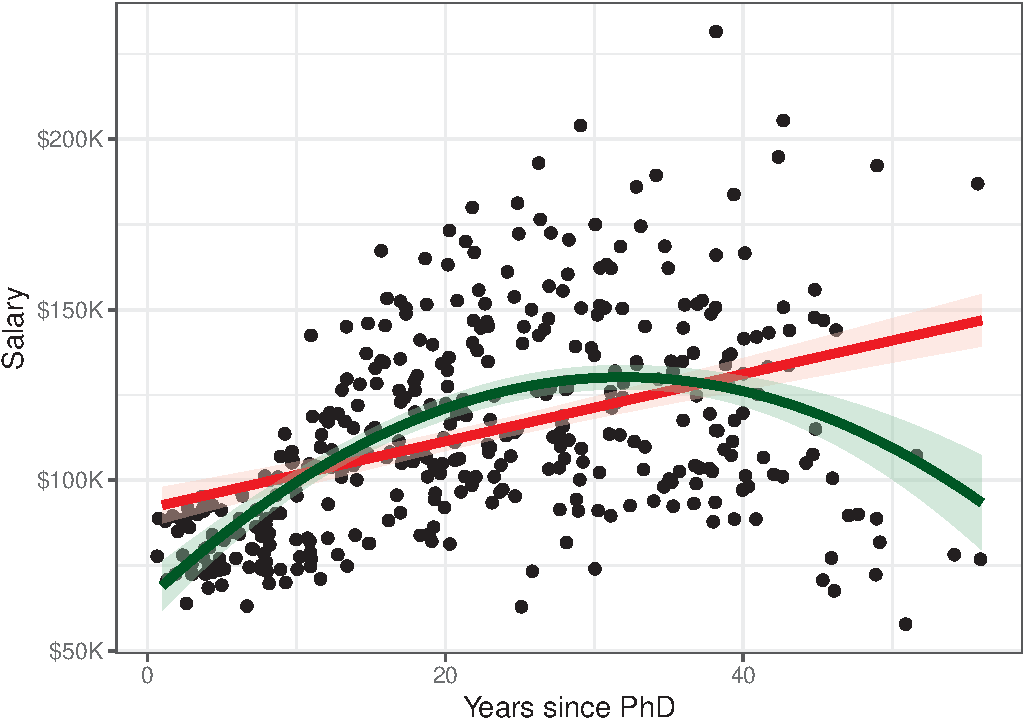
\includegraphics[width=0.8\linewidth,height=\textheight,keepaspectratio]{figs/ch04/fig-Salaries-lm-1.pdf}

}

\caption{\label{fig-Salaries-lm}Scatterplot of Salary vs.~years since
PhD, showing \textcolor{red}{linear} and
\textcolor{darkgreen}{quadratic} smooths with 95\% confidence bands.}

\end{figure}%

This serves to highlight some of our impressions from the basic
scatterplot shown in Figure~\ref{fig-Salaries-scat}, making them more
apparent. And that's precisely the point: the regression smoother draws
attention to a possible pattern that we can consider as a visual summary
of the data. You can think of this as showing what a linear (or
quadratic) regression ``sees'' in the data. Statistical tests can help
you decide if there is more evidence for a quadratic fit compared to the
simpler linear relation.

It is useful to also show some indication of \emph{uncertainty} (or
inversely, \emph{precision}) associated with the predicted values. Both
the linear and quadratic trends are shown in
Figure~\ref{fig-Salaries-lm} with 95\% pointwise confidence
bands.\footnote{Confidence bands allow us to visualize the uncertainty
  around a fitted regression curve. These can be of two types:
  \emph{pointwise intervals} or \emph{simultaneous intervals}. The
  default setting in `\texttt{ggplot2::geom\_smooth()} calculates
  pointwise intervals (using
  \texttt{stats::predict.lm(...,\ interval="confidence")} at a
  confidence level \(1-\alpha\) for the predicted response at \emph{each
  value} \(x_i\) of a predictor, and have the frequentist interpretation
  that over repeated sampling only \(100\;\alpha\) of the predictions at
  \(x_i\) will be outside that interval. In contrast, simultaneous
  intervals are calculated so that \(1 - \alpha\) is the probability
  that \emph{all of them} cover their corresponding true values
  simultaneously. These are necessarily wider than pointwise intervals.
  Commonly used methods for constructing simultaneous confidence bands
  in regression are the Bonferroni and Scheffé methods, which control
  the family-wise error rate over all values of \(x_i\). See
  \href{https://en.wikipedia.org/wiki/Confidence_and_prediction_bands}{}
  for precise definitions of these terms. These are different from a
  \emph{prediction band}, which is used to represent the uncertainty
  about the value of a \textbf{new} data-point on the curve, but subject
  to the additional variance reflected in one observation.} These are
necessarily narrower in the center of the range of \(x\) where there is
typically more data; they get wider toward the highest values of
experience where the data are thinner. \index{uncertainty}
\index{precision}

\subsubsection*{Non-parametric
smoothers}\label{non-parametric-smoothers}
\addcontentsline{toc}{subsubsection}{Non-parametric smoothers}

\index{smoother!non-parametric}

The most generally useful idea is a smoother that tracks an average
value, \(\mathbb{E} (y | x)\), of \(y\) as \(x\) varies across its'
range \emph{without} assuming any particular functional form, and so
avoiding the necessity to choose among
\texttt{y\ \textasciitilde{}\ poly(x,\ 1)}, or
\texttt{y\ \textasciitilde{}\ poly(x,\ 2)}, or
\texttt{y\ \textasciitilde{}\ poly(x,\ 3)}, etc.

Non-parametric smoothers attempt to estimate
\(\mathbb{E} (y | x) = f(x)\) where \(f(x)\) is some smooth function.
These typically use a collection of weighted \emph{local regressions}
for each \(x_i\) within a window centered at that value. In the method
called \emph{lowess} or \emph{loess}
(\citeproc{ref-Cleveland:79}{Cleveland, 1979};
\citeproc{ref-ClevelandDevlin:88}{Cleveland \& Devlin, 1988}), a weight
function is applied, giving greatest weight to \(x_i\) and a weight of 0
outside a window containing a certain fraction, \(s\), called
\emph{span}, of the nearest neighbors of \(x_i\). The fraction, \(s\),
is usually within the range \(1/3 \le s \le 2/3\), and it determines the
smoothness of the resulting curve; smaller values produce a wigglier
curve and larger values giving a smoother fit (an optimal span can be
determined by \(k\)-fold cross-validation to minimize a measure of
overall error of approximation).

Non-parametric regression is a broad topic; see Fox
(\citeproc{ref-Fox:2016:ARA}{2016}), Ch. 18 for a more general treatment
including smoothing splines, and Wood (\citeproc{ref-Wood:2006}{2006})
for generalized additive models, fit using \texttt{method\ =\ "gam"} in
\textbf{ggplot2}, which is the default when the largest group has more
than 1,000 observations.

Figure~\ref{fig-Salaries-loess} shows the addition of a loess smooth to
the plot in Figure~\ref{fig-Salaries-lm}, suppressing the confidence
band for the linear regression. The loess fit is nearly coincident with
the quadratic fit, but has a slightly wider confidence band.

\begin{Shaded}
\begin{Highlighting}[]
\NormalTok{gg1 }\SpecialCharTok{+} 
  \FunctionTok{geom\_smooth}\NormalTok{(}\AttributeTok{method =} \StringTok{"loess"}\NormalTok{, }\AttributeTok{formula =} \StringTok{"y \textasciitilde{} x"}\NormalTok{, }
              \AttributeTok{color =} \StringTok{"blue"}\NormalTok{, }\AttributeTok{fill =}\NormalTok{ scales}\SpecialCharTok{::}\FunctionTok{muted}\NormalTok{(}\StringTok{"blue"}\NormalTok{),}
              \AttributeTok{linewidth =} \DecValTok{2}\NormalTok{) }\SpecialCharTok{+}
  \FunctionTok{geom\_smooth}\NormalTok{(}\AttributeTok{method =} \StringTok{"lm"}\NormalTok{, }\AttributeTok{formula =} \StringTok{"y \textasciitilde{} x"}\NormalTok{, }\AttributeTok{se =} \ConstantTok{FALSE}\NormalTok{,}
              \AttributeTok{color =} \StringTok{"red"}\NormalTok{,}
              \AttributeTok{linewidth =} \DecValTok{2}\NormalTok{) }\SpecialCharTok{+}
  \FunctionTok{geom\_smooth}\NormalTok{(}\AttributeTok{method =} \StringTok{"lm"}\NormalTok{, }\AttributeTok{formula =} \StringTok{"y \textasciitilde{} poly(x,2)"}\NormalTok{, }
              \AttributeTok{color =} \StringTok{"darkgreen"}\NormalTok{, }\AttributeTok{fill =} \StringTok{"lightgreen"}\NormalTok{,}
              \AttributeTok{linewidth =} \DecValTok{2}\NormalTok{) }
\end{Highlighting}
\end{Shaded}

\begin{figure}[htb!]

\centering{

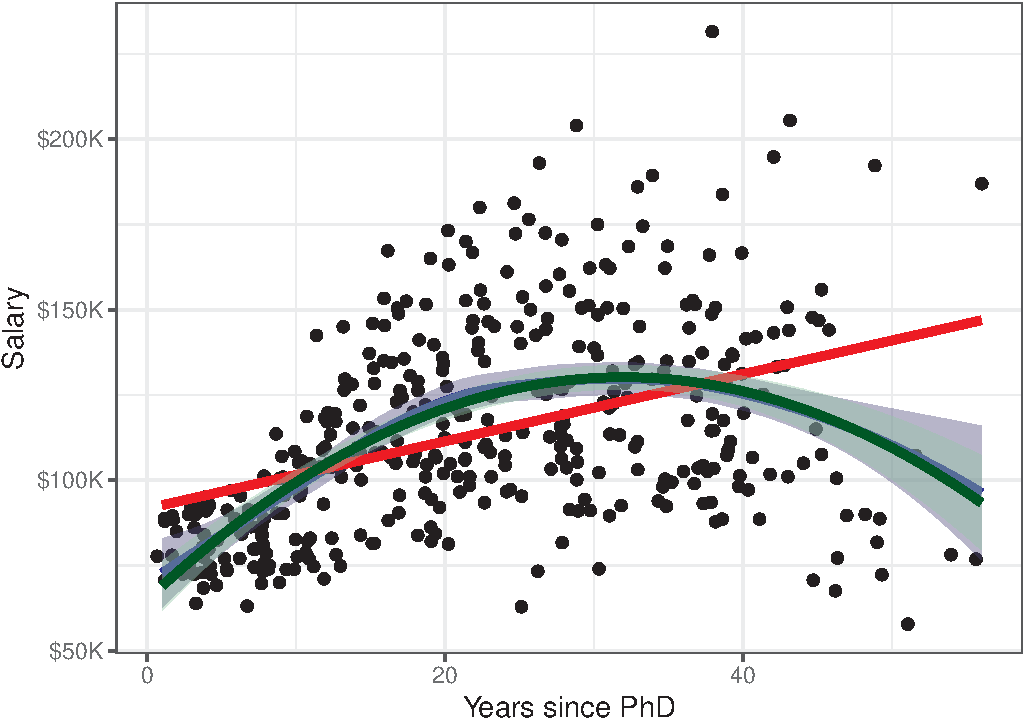
\includegraphics[width=0.8\linewidth,height=\textheight,keepaspectratio]{figs/ch04/fig-Salaries-loess-1.pdf}

}

\caption{\label{fig-Salaries-loess}Scatterplot of Salary vs.~years since
PhD, adding the loess smooth. The loess smooth curve and confidence band
in \textcolor{green}{green} is nearly indistinguishable from a quadratic
fit in \textcolor{blue}{blue}.}

\end{figure}%

But now comes an important question: is it reasonable that academic
salary should increase up to about 40 years since the PhD degree and
then decline? The predicted salary for someone still working 50 years
after earning their degree is about the same as a person at 15 years.
What else is going on here?

\index{smoother|)}

\subsection{Stratifiers}\label{stratifiers}

\index{stratifier|(}

Very often, we have a main relationship of interest, but various groups
in the data are identified by discrete factors (like faculty
\texttt{rank} and \texttt{sex}, their type of \texttt{discipline} here),
or there are quantitative predictors for which the main relation might
vary. In the language of statistical models such effects are
\emph{interaction} terms, as in
\texttt{y\ \textasciitilde{}\ group\ +\ x\ +\ group:x}, where the term
\texttt{group:x} fits a different slope for each group and the grouping
variable is often called a \emph{moderator} variable. Common moderator
variables are ethnicity, health status, social class and level of
education. Moderators can also be continuous variables as in
\texttt{y\ \textasciitilde{}\ x1\ +\ x2\ +\ x1:x2}.

I call these \emph{stratifiers}, recognizing that we should consider
breaking down the overall relation to see whether and how it changes
over such ``other'' variables. Such variables are most often factors,
but we can cut a continuous variable into ranges (\emph{shingles}) and
do the same graphically. There are two general graphical techniques for
stratifying:

\begin{itemize}
\item
  \textbf{Grouping}: Identify subgroups in the data by assigning
  different visual attributes, such as color, shape, line style, etc.
  within a single plot, as shown in Figure~\ref{fig-Salaries-rank}
  below. This is quite natural for factors; quantitative predictors can
  be accommodated by cutting their range into ordered intervals.
  Grouping has the advantage that the levels of a grouping variable can
  be shown within the same plot, facilitating direct comparison.
\item
  \textbf{Conditioning}: Showing subgroups in different plot panels, as
  in Figure~\ref{fig-Salaries-faceted}. This has the advantages that
  relations for the individual groups more easily discerned and one can
  easily stratify by two (or more) other variables jointly. But visual
  comparison is more difficult because the eye must scan from one panel
  to another.
\end{itemize}

\begin{tcolorbox}[enhanced jigsaw, titlerule=0mm, bottomtitle=1mm, left=2mm, opacityback=0, bottomrule=.15mm, breakable, colframe=quarto-callout-note-color-frame, toptitle=1mm, rightrule=.15mm, opacitybacktitle=0.6, colbacktitle=quarto-callout-note-color!10!white, leftrule=.75mm, coltitle=black, arc=.35mm, title=\textcolor{quarto-callout-note-color}{\faInfo}\hspace{0.5em}{History Corner: Coplots and faceting}, toprule=.15mm, colback=white]

The syntax you use in specifying a plot plays an important role in
visual thinking. Ideally, you want the shortest path between having a
graphic idea in your head and specifying that in code to see the result
rendered on your screen. \index{visual thinking}

Recognition of the roles of visual grouping by factors within a panel
and conditioning in multi-panel displays was an important advance in the
development of modern statistical graphics software. It began at A.T.\&
T. Bell Labs in Murray Hill, NJ in conjunction with the \textbf{S}
language, the mother of R.

Conditioning displays (originally called \emph{coplots}
(\citeproc{ref-ChambersHastie1991}{Chambers \& Hastie, 1991})) are
simply a collection of 1D, 2D or 3D plots separate panels for subsets of
the data broken down by one or more factors, or, for quantitative
variables, subdivided into a factor with several overlapping intervals
(\emph{shingles}). The first implementation was in \emph{Trellis} plots
(\citeproc{ref-Becker:1996:VDC}{Becker et al., 1996};
\citeproc{ref-Cleveland:85}{Cleveland, 1985}). \index{trellis plots}

Trellis displays were extended in the
\textcolor{brown}{\texttt{\textbf{lattice}}} package
(\citeproc{ref-R-lattice}{Sarkar, 2008}) %
   \index{lattice@\texttt{lattice} package}%
   \index{packages!lattice@\texttt{lattice}}%
     , which offered:

\begin{itemize}
\tightlist
\item
  A \textbf{graphing syntax} similar to that used in statistical model
  formulas: \texttt{y\ \textasciitilde{}\ x\ \textbar{}\ g} conditions
  the data by the levels of \texttt{g}, with \texttt{\textbar{}} read as
  ``given''; two or more conditioning are specified as
  \texttt{y\ \textasciitilde{}\ x\ \textbar{}\ g1\ +\ g2\ +\ ...}, with
  \texttt{+} read as ``and''.
\item
  \textbf{Panel functions} define what is plotted in a given panel.
  \texttt{panel.xyplot()} is the default for scatterplots, plotting
  points, but you can add \texttt{panel.lmline()} for regression lines,
  \texttt{latticeExtra::panel.smoother()} for loess smooths and a wide
  variety of others.
\end{itemize}

The \textcolor{brown}{\texttt{\textbf{car}}} package
(\citeproc{ref-R-car}{Fox \& Weisberg, 2019}) %
   \index{car@\texttt{car} package}%
   \index{packages!car@\texttt{car}}%
     supports this graphing syntax in many of its functions.
\textcolor{brown}{\texttt{\textbf{ggplot2}}} %
   \index{ggplot2@\texttt{ggplot2} package}%
   \index{packages!ggplot2@\texttt{ggplot2}}%
     does not; it uses aesthetics (\texttt{aes()}), which map variables
in the data to visual characteristics in displays.

\end{tcolorbox}

\textbf{Using grouping} For the \texttt{Salaries} data, the most obvious
variable that affects academic salary is \texttt{rank}, because faculty
typically get an increase in salary with a promotion that carries
through in their future salary. What can we see if we group by
\texttt{rank} and fit a separate smoothed curve for each?

In \texttt{ggplot2} thinking, grouping is accomplished simply by adding
an aesthetic, such as \texttt{color\ =\ rank}. What happens then is that
points, lines, smooths and other \texttt{geom\_*()} inherit the feature
that they are differentiated by color. In the case of
\texttt{geom\_smooth()}, we get a separate fit for each subset of the
data, according to \texttt{rank}.

\begin{Shaded}
\begin{Highlighting}[]
\CommentTok{\# make some re{-}useable pieces to avoid repetitions}
\NormalTok{scale\_salary }\OtherTok{\textless{}{-}}   \FunctionTok{scale\_y\_continuous}\NormalTok{(}
  \AttributeTok{labels =}\NormalTok{ scales}\SpecialCharTok{::}\FunctionTok{dollar\_format}\NormalTok{(}\AttributeTok{prefix=}\StringTok{"$"}\NormalTok{, }
                                 \AttributeTok{scale =} \FloatTok{0.001}\NormalTok{, }
                                 \AttributeTok{suffix =} \StringTok{"K"}\NormalTok{)) }
\CommentTok{\# position the legend inside the plot}
\NormalTok{legend\_pos }\OtherTok{\textless{}{-}} \FunctionTok{theme}\NormalTok{(}\AttributeTok{legend.position =} \StringTok{"inside"}\NormalTok{,}
                    \AttributeTok{legend.position.inside =} \FunctionTok{c}\NormalTok{(.}\DecValTok{1}\NormalTok{, }\FloatTok{0.95}\NormalTok{), }
                    \AttributeTok{legend.justification =} \FunctionTok{c}\NormalTok{(}\DecValTok{0}\NormalTok{, }\DecValTok{1}\NormalTok{))}

\FunctionTok{ggplot}\NormalTok{(Salaries, }
       \FunctionTok{aes}\NormalTok{(}\AttributeTok{x =}\NormalTok{ yrs.since.phd, }\AttributeTok{y =}\NormalTok{ salary, }
           \AttributeTok{color =}\NormalTok{ rank, }\AttributeTok{shape =}\NormalTok{ rank)) }\SpecialCharTok{+}
  \FunctionTok{geom\_point}\NormalTok{() }\SpecialCharTok{+}
\NormalTok{  scale\_salary }\SpecialCharTok{+}
  \FunctionTok{labs}\NormalTok{(}\AttributeTok{x =} \StringTok{"Years since PhD"}\NormalTok{,}
       \AttributeTok{y =} \StringTok{"Salary"}\NormalTok{) }\SpecialCharTok{+}
  \FunctionTok{geom\_smooth}\NormalTok{(}\FunctionTok{aes}\NormalTok{(}\AttributeTok{fill =}\NormalTok{ rank),}
                  \AttributeTok{method =} \StringTok{"loess"}\NormalTok{, }\AttributeTok{formula =} \StringTok{"y \textasciitilde{} x"}\NormalTok{, }
                  \AttributeTok{linewidth =} \DecValTok{2}\NormalTok{)  }\SpecialCharTok{+}
\NormalTok{  legend\_pos}
\end{Highlighting}
\end{Shaded}

\begin{figure}[htb!]

\centering{

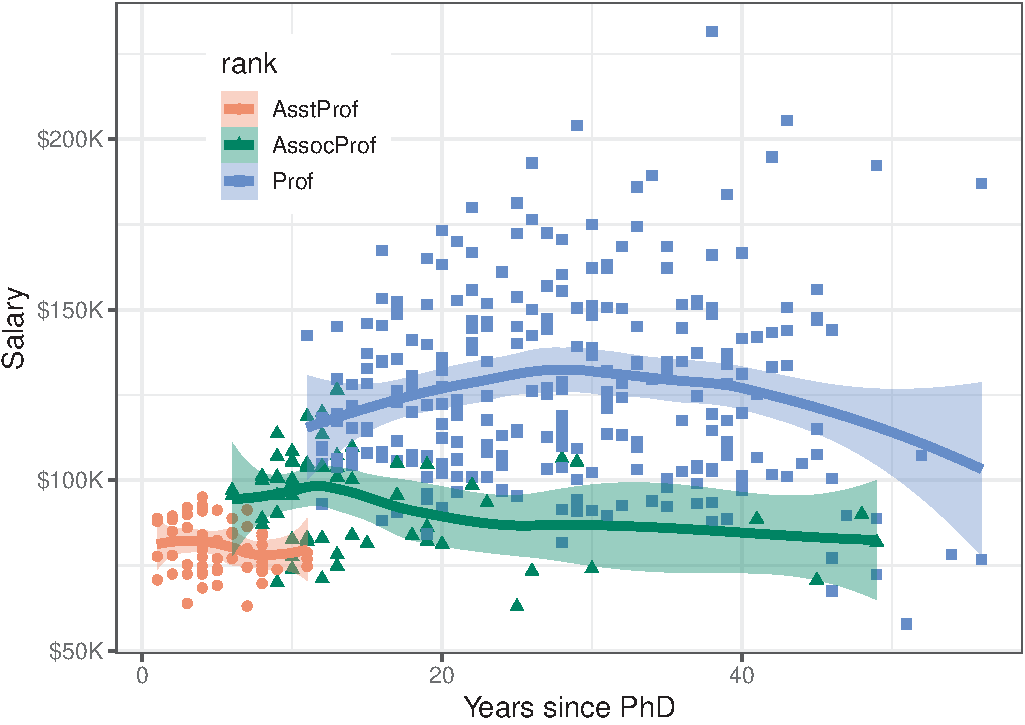
\includegraphics[width=0.8\linewidth,height=\textheight,keepaspectratio]{figs/ch04/fig-Salaries-rank-1.pdf}

}

\caption{\label{fig-Salaries-rank}Scatterplot of Salary vs.~years since
PhD, grouped by rank.}

\end{figure}%

Well, there is a different story here. Salaries generally occupy
separate vertical levels, increasing with academic rank. The horizontal
extents of the smoothed curves show their ranges. Within each rank there
is some initial increase after promotion, and then some tendency to
decline with increasing years. But, by and large, years since the PhD
doesn't make as much difference once we've taken academic rank into
account.

What about the \texttt{discipline} which is classified, perhaps
peculiarly, as ``theoretical'' vs.~``applied''? The values are just
\texttt{"A"} and \texttt{"B"}, so I map these to more meaningful labels
before making the plot.

\begin{Shaded}
\begin{Highlighting}[]
\NormalTok{Salaries }\OtherTok{\textless{}{-}}\NormalTok{ Salaries }\SpecialCharTok{|\textgreater{}}
  \FunctionTok{mutate}\NormalTok{(}\AttributeTok{discipline =} 
           \FunctionTok{factor}\NormalTok{(discipline, }
                  \AttributeTok{labels =} \FunctionTok{c}\NormalTok{(}\StringTok{"A: Theoretical"}\NormalTok{, }\StringTok{"B: Applied"}\NormalTok{)))}

\NormalTok{Salaries }\SpecialCharTok{|\textgreater{}}
  \FunctionTok{ggplot}\NormalTok{(}\FunctionTok{aes}\NormalTok{(}\AttributeTok{x =}\NormalTok{ yrs.since.phd, }\AttributeTok{y =}\NormalTok{ salary, }\AttributeTok{color =}\NormalTok{ discipline)) }\SpecialCharTok{+}
    \FunctionTok{geom\_point}\NormalTok{() }\SpecialCharTok{+}
\NormalTok{  scale\_salary }\SpecialCharTok{+}
  \FunctionTok{geom\_smooth}\NormalTok{(}\FunctionTok{aes}\NormalTok{(}\AttributeTok{fill =}\NormalTok{ discipline ),}
                \AttributeTok{method =} \StringTok{"loess"}\NormalTok{, }\AttributeTok{formula =} \StringTok{"y \textasciitilde{} x"}\NormalTok{, }
                \AttributeTok{linewidth =} \DecValTok{2}\NormalTok{) }\SpecialCharTok{+} 
  \FunctionTok{labs}\NormalTok{(}\AttributeTok{x =} \StringTok{"Years since PhD"}\NormalTok{,}
       \AttributeTok{y =} \StringTok{"Salary"}\NormalTok{) }\SpecialCharTok{+}
\NormalTok{  legend\_pos }
\end{Highlighting}
\end{Shaded}

\begin{figure}[htb!]

\centering{

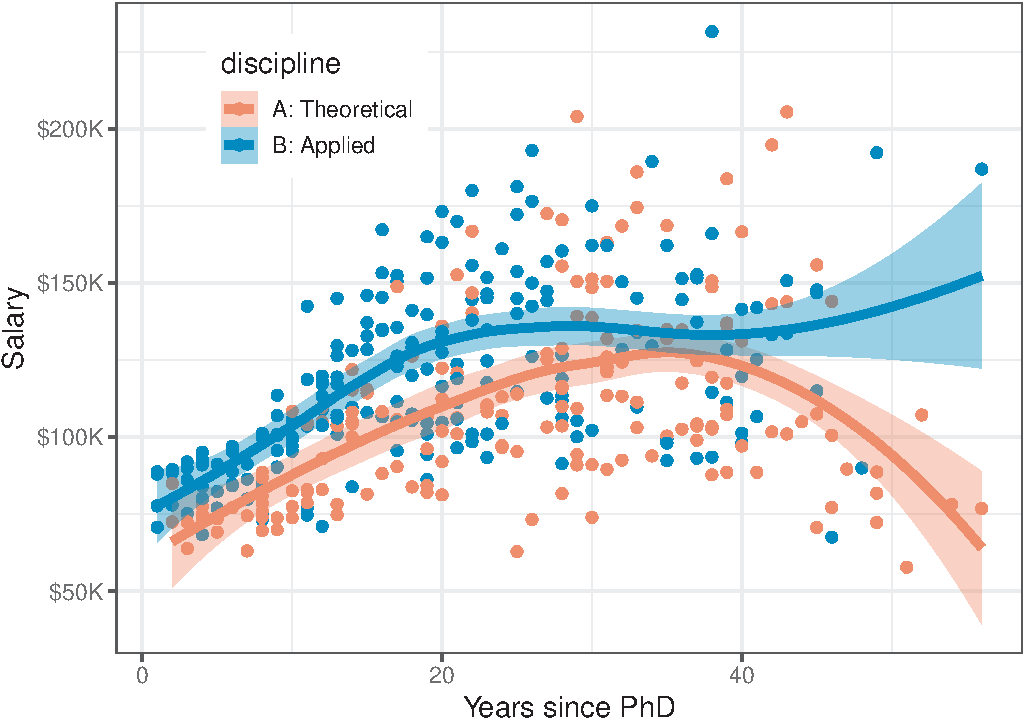
\includegraphics[width=0.8\linewidth,height=\textheight,keepaspectratio]{figs/ch04/fig-Salaries-discipline-1.pdf}

}

\caption{\label{fig-Salaries-discipline}Scatterplot of Salary vs.~years
since PhD, grouped by discipline.}

\end{figure}%

The story in Figure~\ref{fig-Salaries-discipline} is again different.
Faculty in applied disciplines on average earn about 10,000\$ more per
year on average than their theoretical colleagues.

\begin{Shaded}
\begin{Highlighting}[]
\NormalTok{Salaries }\SpecialCharTok{|\textgreater{}}
  \FunctionTok{group\_by}\NormalTok{(discipline) }\SpecialCharTok{|\textgreater{}}
  \FunctionTok{summarize}\NormalTok{(}\AttributeTok{mean =} \FunctionTok{mean}\NormalTok{(salary)) }
\CommentTok{\# \# A tibble: 2 x 2}
\CommentTok{\#   discipline        mean}
\CommentTok{\#   \textless{}fct\textgreater{}            \textless{}dbl\textgreater{}}
\CommentTok{\# 1 A: Theoretical 108548.}
\CommentTok{\# 2 B: Applied     118029.}
\end{Highlighting}
\end{Shaded}

For both groups, there is an approximately linear relation up to about
30--40 years, but the smoothed curves then diverge into the region where
the data is thinner.

This result is more surprising than differences among faculty ranks. The
effect of annotation with smoothed curves as visual summaries is
apparent, and provides a stimulus to think about \emph{why} these
differences (if they are real) exist between theoretical and applied
professors, and maybe \emph{should} theoreticians be paid more!

\subsection{Conditioning}\label{conditioning}

\index{conditioning|(}
\index{faceting}

The previous plots use grouping by color to plot the data for different
subsets inside the same plot window, making comparison among groups
easier, because they can be directly compared along a common vertical
scale \footnote{The classic study by Cleveland \& McGill
  (\citeproc{ref-ClevelandMcGill:84b}{1984});Cleveland \& McGill
  (\citeproc{ref-ClevelandMcGill:85}{1985}) shows that judgements of
  magnitude along a common scale are more accurate than those along
  separate, aligned scales.}. This gets messy, however, when there are
more than just a few levels, or worse---when there are two (or more)
variables for which we want to show separate effects. In such cases, we
can plot separate panels using the \texttt{ggplot2} concept of
\emph{faceting}. There are two options: \texttt{facet\_wrap()} takes one
or more conditioning variables and produces a ribbon of plots for each
combination of levels; \texttt{facet\_grid(row\ \textasciitilde{}\ col)}
takes two or more conditioning variables and arranges the plots in a 2D
array identified by the \texttt{row} and \texttt{col} variables.

Let's look at salary broken down by the combinations of discipline and
rank. Here, I chose to stratify using color by rank within each of
panels faceting by discipline. Because there is more going on in this
plot, a linear smooth is used to represent the trend.

\begin{Shaded}
\begin{Highlighting}[]
\NormalTok{Salaries }\SpecialCharTok{|\textgreater{}}
  \FunctionTok{ggplot}\NormalTok{(}\FunctionTok{aes}\NormalTok{(}\AttributeTok{x =}\NormalTok{ yrs.since.phd, }\AttributeTok{y =}\NormalTok{ salary, }
             \AttributeTok{color =}\NormalTok{ rank, }\AttributeTok{shape =}\NormalTok{ rank)) }\SpecialCharTok{+}
  \FunctionTok{geom\_point}\NormalTok{() }\SpecialCharTok{+}
\NormalTok{  scale\_salary }\SpecialCharTok{+}
  \FunctionTok{labs}\NormalTok{(}\AttributeTok{x =} \StringTok{"Years since PhD"}\NormalTok{,}
       \AttributeTok{y =} \StringTok{"Salary"}\NormalTok{) }\SpecialCharTok{+}
  \FunctionTok{geom\_smooth}\NormalTok{(}\FunctionTok{aes}\NormalTok{(}\AttributeTok{fill =}\NormalTok{ rank),}
              \AttributeTok{method =} \StringTok{"lm"}\NormalTok{, }\AttributeTok{formula =} \StringTok{"y \textasciitilde{} x"}\NormalTok{, }
              \AttributeTok{linewidth =} \DecValTok{2}\NormalTok{, }\AttributeTok{alpha =} \DecValTok{1}\SpecialCharTok{/}\DecValTok{4}\NormalTok{) }\SpecialCharTok{+}
  \FunctionTok{facet\_wrap}\NormalTok{(}\SpecialCharTok{\textasciitilde{}}\NormalTok{ discipline) }\SpecialCharTok{+}
\NormalTok{  legend\_pos}
\end{Highlighting}
\end{Shaded}

\begin{figure}[htb!]

\centering{

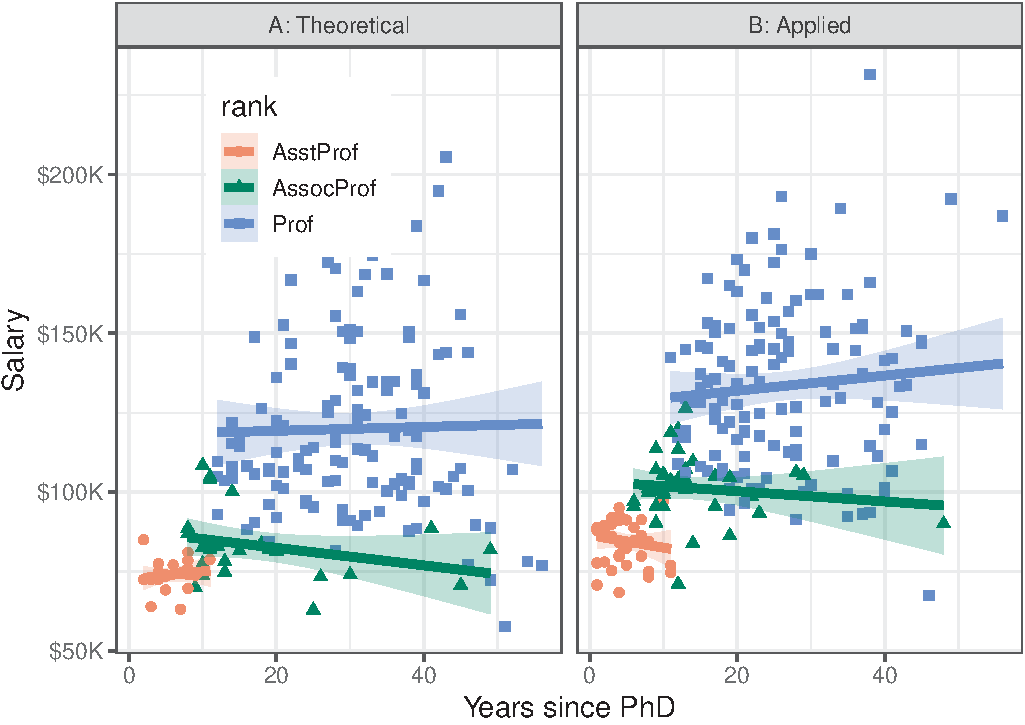
\includegraphics[width=0.9\linewidth,height=\textheight,keepaspectratio]{figs/ch04/fig-Salaries-faceted-1.pdf}

}

\caption{\label{fig-Salaries-faceted}Scatterplot of Salary vs.~years
since PhD, grouped by rank, with separate panels for discipline.}

\end{figure}%

Once both of these factors are taken into account, there does not seem
to be much impact of years of service. Salaries in theoretical
disciplines are noticeably greater than those in applied disciplines at
all ranks, and there are even greater differences among ranks.

Finally, to shed light on the question that motivated this example---
are there anomalous differences in salary for men and women--- we can
look at differences in salary according to sex, when discipline and rank
are taken into account. To do this graphically, condition by both
variables, but use
\texttt{facet\_grid(discipline\ \textasciitilde{}\ rank)} to arrange
their combinations in a grid whose rows are the levels of
\texttt{discipline} and columns are those of \texttt{rank}. I want to
make the comparison of males and females most direct, so I use
\texttt{color\ =\ sex} to stratify the panels. The smoothed regression
lines and error bands are calculated separately for each combination of
discipline, rank and sex.

\begin{Shaded}
\begin{Highlighting}[]
\NormalTok{Salaries }\SpecialCharTok{|\textgreater{}}
  \FunctionTok{ggplot}\NormalTok{(}\FunctionTok{aes}\NormalTok{(}\AttributeTok{x =}\NormalTok{ yrs.since.phd, }\AttributeTok{y =}\NormalTok{ salary, }\AttributeTok{color =}\NormalTok{ sex)) }\SpecialCharTok{+}
  \FunctionTok{geom\_point}\NormalTok{() }\SpecialCharTok{+}
\NormalTok{  scale\_salary }\SpecialCharTok{+}
  \FunctionTok{labs}\NormalTok{(}\AttributeTok{x =} \StringTok{"Years since PhD"}\NormalTok{,}
       \AttributeTok{y =} \StringTok{"Salary"}\NormalTok{) }\SpecialCharTok{+}
  \FunctionTok{geom\_smooth}\NormalTok{(}\FunctionTok{aes}\NormalTok{(}\AttributeTok{fill =}\NormalTok{ sex),}
              \AttributeTok{method =} \StringTok{"lm"}\NormalTok{, }\AttributeTok{formula =} \StringTok{"y \textasciitilde{} x"}\NormalTok{,}
              \AttributeTok{linewidth =} \DecValTok{2}\NormalTok{, }\AttributeTok{alpha =} \DecValTok{1}\SpecialCharTok{/}\DecValTok{4}\NormalTok{) }\SpecialCharTok{+}
  \FunctionTok{facet\_grid}\NormalTok{(discipline }\SpecialCharTok{\textasciitilde{}}\NormalTok{ rank) }\SpecialCharTok{+}
\NormalTok{  legend\_pos}
\end{Highlighting}
\end{Shaded}

\begin{figure}[htb!]

\centering{

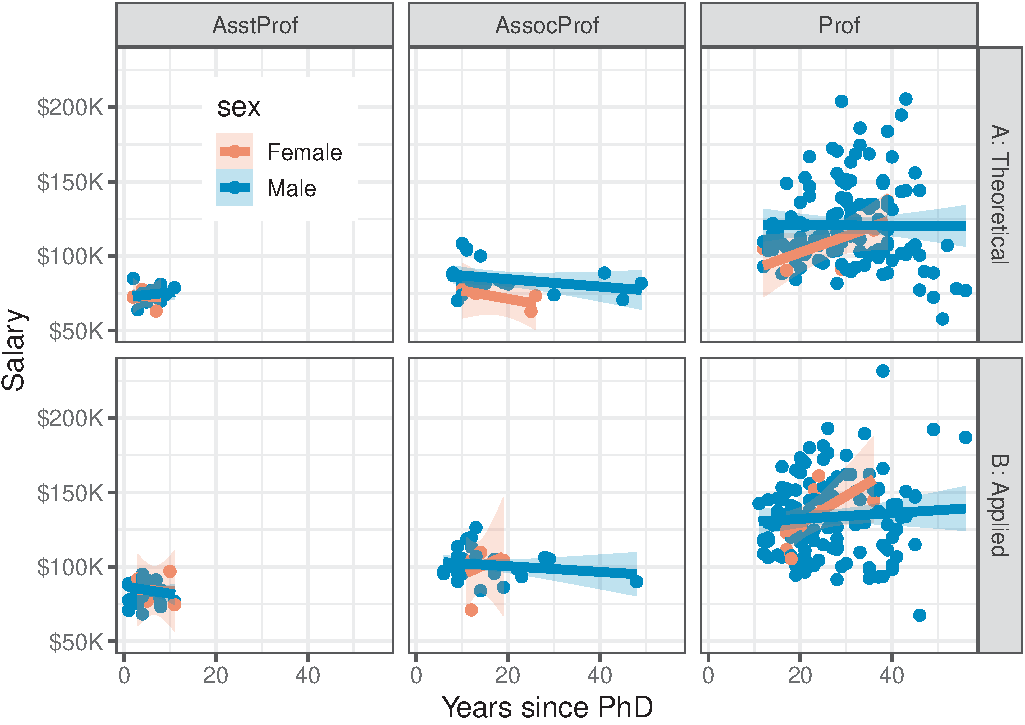
\includegraphics[width=0.9\linewidth,height=\textheight,keepaspectratio]{figs/ch04/fig-Salaries-facet-sex-1.pdf}

}

\caption{\label{fig-Salaries-facet-sex}Scatterplot of Salary vs.~years
since PhD, grouped by sex, faceted by discipline and rank.}

\end{figure}%

\index{conditioning|)}
\index{stratifier|)}

\section{Data Ellipses}\label{sec-data-ellipse}

\index{data ellipse|(}

The \emph{data ellipse} (\citeproc{ref-Monette:90}{Monette, 1990}), or
\emph{concentration ellipse} (\citeproc{ref-Dempster:69}{Dempster,
1969}) is a remarkably simple and effective display for viewing and
understanding bivariate relationships in multivariate data. The data
ellipse is typically used to add a visual summary to a scatterplot, that
shows all together the means, standard deviations, correlation, and
slope of the regression line for two variables, perhaps stratified by
another variable.

Under the classical assumption that the data are bivariate normally
distributed, the data ellipse is also a \textbf{sufficient} visual
summary, in the sense that it captures \textbf{all} relevant features of
the data. See Friendly et al.
(\citeproc{ref-Friendly-etal:ellipses:2013}{2013}) for a complete
discussion of the role of ellipsoids in statistical data visualization.

The data ellipse is based on the idea that in a bivariate normal
distribution, the contours of equal probability form a series of
concentric ellipses. If the variables were uncorrelated and had the same
variances, these would be circles, and Euclidean distance would measure
the distance of each observation from the mean. When the variables are
correlated, a different measure, \emph{Mahalanobis distance} is the
proper measure of how far a point is from the mean, taking the
correlation into account. \index{Mahalanobis distance}

\begin{figure}[htb!]

\centering{

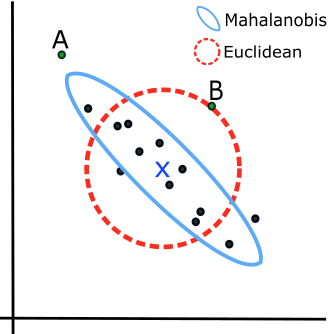
\includegraphics[width=0.5\linewidth,height=\textheight,keepaspectratio]{images/mahalanobis.png}

}

\caption{\label{fig-mahalanobis}2D data with curves of constant distance
from the centroid. The blue solid ellipse shows a contour of constant
Mahalanobis distance, taking the correlation into account; the dashed
red circle is a contour of equal Euclidean distance. Given the data
points, which of the points \textbf{A} and \textbf{B} is further from
the mean (X)? \emph{Source}: Re-drawn from
\href{https://ouzhang.rbind.io/2020/11/16/outliers-part4/}{Ou Zhang}}

\end{figure}%

To illustrate, Figure~\ref{fig-mahalanobis} shows a scatterplot with
labels for two points, ``A'' and ``B''. Which is further from the mean,
``X''? A contour of constant Euclidean distance, shown by the
\textcolor{red}{red} dashed circle, ignores the apparent negative
correlation, so point ``A'' is further. The \textcolor{blue}{blue}
ellipse for Mahalanobis distance takes the correlation into account, so
point ``B'' has a greater distance from the mean.

Mathematically, Euclidean (squared) distance (\(D_E^2(y)\)) for \(p\)
variables, \(j = 1, 2, \dots , p\), is just a generalization of the
square of a univariate standardized (\(z\)) score,
\(z^2 = [(y - \bar{y}) / s]^2\),

\[
D_E^2 (\mathbf{y}) = \sum_j^p z_j^2 = \mathbf{z}^\textsf{T}  \mathbf{z} = (\mathbf{y} - \bar{\mathbf{y}})^\textsf{T} \operatorname{diag}(\mathbf{S})^{-1} (\mathbf{y} - \bar{\mathbf{y}}) \; ,
\] where \(\mathbf{S}\) is the sample variance-covariance matrix,
\(\mathbf{S} = ({n-1})^{-1} \sum_{i=1}^n (\mathbf{y}_i - \bar{\mathbf{y}})^\textsf{T} (\mathbf{y}_i - \bar{\mathbf{y}})\).

Mahalanobis distance takes the correlations into account simply by using
the covariances as well as the variances,

\begin{equation}\phantomsection\label{eq-Dsq}{
D_M^2 (\mathbf{y}) = (\mathbf{y} - \bar{\mathbf{y}})^\mathsf{T} S^{-1} (\mathbf{y} - \bar{\mathbf{y}}) \; .
}\end{equation}

In Equation~\ref{eq-Dsq}, the inverse \(S^{-1}\) serves to ``divide''
the matrix
\((\mathbf{y} - \bar{\mathbf{y}})^\mathsf{T} (\mathbf{y} - \bar{\mathbf{y}})\)
of squared distances by the variances (and covariances) of the
variables, as in the univariate case.

For \(p\) variables, the data \emph{ellipsoid} \(\mathcal{E}_c\) of size
\(c\) is a \(p\)-dimensional ellipse, defined as the set of points
\(\mathbf{y} = (y_1, y_2, \dots y_p)\) whose squared Mahalanobis
distance, \(D_M^2 ( \mathbf{y} )\) is less than or equal to \(c^2\),

\[
\mathcal{E}_c (\bar{\mathbf{y}}, \mathbf{S}) := \{ D_M^2 (\mathbf{y}) \le c^2 \} \; .
\]

\subsection{Drawing data ellipses}\label{drawing-data-ellipses}

A computational definition of the data ellipsoid recognizes that the
boundary of an ellipsoid can be found by (a) starting with a unit a unit
sphere \(\mathcal{P}\) centered at the origin, (b) transforming that by
a ``square root'' of the covariance matrix, denoted
\(\mathbf{S}^{1/2}\), and then (c) shifting that to centroid of the
data.

The unit sphere is defined as the contour of Euclidean distance 1 from
the origin, \(\mathcal{P} := \{ \mathbf{x}^\textsf{T} \mathbf{x}= 1\}\).
Using the notation \(\oplus\) to represent translation to a new centroid
at the variable means, \(\bar{\mathbf{y}}\), the data ellipsoid becomes,

\[
\mathcal{E}_c (\bar{\mathbf{y}}, \mathbf{S}) = \bar{\mathbf{y}} \; \oplus \; \mathbf{S}^{1/2} \, \mathcal{P} \:\: .
\] The matrix \(\mathbf{S}^{1/2}\) represents a rotation and scaling of
the sphere and is commonly computed as the Cholesky factor of
\(\mathbf{S}\) given in R by \texttt{chol(S)}. You can imagine this in
2D by thinking of how the dashed \textcolor{red}{red} circle in
Figure~\ref{fig-mahalanobis} could be transformed into the
\textcolor{blue}{blue} ellipse.

Slightly abusing notation and taking the unit sphere \(\mathcal{P}\)
like an identity matrix \(\mathbf{I}\) that vanishes in multiplication,
we can write the data ellipsoid as simply:

\begin{equation}\phantomsection\label{eq-ellE}{
\mathcal{E}_c (\bar{\mathbf{y}}, \mathbf{S}) = \bar{\mathbf{y}} \; \oplus \; c\, \sqrt{\mathbf{S}} \:\: .
}\end{equation}

\textbf{Contour levels (\(c\))}

When \(\mathbf{y}\) is (at least approximately) bivariate normal,
\(D_M^2(\mathbf{y})\) has a large-sample \(\chi^2_2\) distribution
(\(\chi^2\) with 2 df), so ellipses of various conventional sizes can be
calculated using \texttt{qchisq()}:

\begin{itemize}
\tightlist
\item
  \(c^2 = \chi^2_2 (0.5) = 1.39\) gives a data ellipse covering 50\% of
  the data points, a bivariate analog of the central box of a boxplot.
\item
  \(c^2 = \chi^2_2 (0.68) = 2.28\) gives a ``1 standard deviation
  bivariate ellipse,'' an analog of the standard interval
  \(\bar{y} \pm 1 s\),
\item
  \(c^2 = \chi^2_2 (0.95) = 5.99 \approx 6\) gives a data ellipse of
  95\% coverage.
\end{itemize}

In not-large samples, the radius \(c\) of the ellipsoid is better
approximated by a multiple of a \(F_{p, n-p}\) distribution, with \(p\)
variables and \(n-p\) degrees of freedom for \(\mathbf{S}\). This gives
a radius \(c =\sqrt{ 2 F_{2, n-2}^{1-\alpha} }\) in the bivariate case
(\(p=2\)) for coverage \(1-\alpha\).

These three conventional cases are illustrated in
Figure~\ref{fig-ellipses-coverage} with ellipses of 50\%, 68\% and 95\%
coverage for a the matrix \(\mathbf{S}\) defined below and
\(\bar{\mathbf{y}} = \mathbf{0}\). Here, the variance of
\(\mathbf{y}_1\) is twice that of \(\mathbf{y}_2\) and the correlation
works out to \(r(y_1, y_2) = 0.35\).

\begin{Shaded}
\begin{Highlighting}[]
\NormalTok{ybar }\OtherTok{\textless{}{-}} \FunctionTok{c}\NormalTok{(}\DecValTok{0}\NormalTok{, }\DecValTok{0}\NormalTok{)}
\NormalTok{S }\OtherTok{\textless{}{-}} \FunctionTok{matrix}\NormalTok{(}\FunctionTok{c}\NormalTok{(}\DecValTok{1}\NormalTok{, .}\DecValTok{5}\NormalTok{, .}\DecValTok{5}\NormalTok{, }\DecValTok{2}\NormalTok{), }\DecValTok{2}\NormalTok{, }\DecValTok{2}\NormalTok{)}
\FunctionTok{rownames}\NormalTok{(S) }\OtherTok{\textless{}{-}} \FunctionTok{colnames}\NormalTok{(S) }\OtherTok{\textless{}{-}} \FunctionTok{c}\NormalTok{(}\StringTok{"y1"}\NormalTok{, }\StringTok{"y2"}\NormalTok{)}
\NormalTok{S}
\CommentTok{\#     y1  y2}
\CommentTok{\# y1 1.0 0.5}
\CommentTok{\# y2 0.5 2.0}
\end{Highlighting}
\end{Shaded}

Statistical ellipses are conveniently drawn using
\texttt{car::ellipse()}. \texttt{heplots::ellipse.label()} provides
flexible ways to add labels to ellipses at various locations around the
ellipse shown in Figure~\ref{fig-ellipses-coverage}. These are called
repeatedly to overlay the three ellipses.

\begin{Shaded}
\begin{Highlighting}[]
\NormalTok{levels }\OtherTok{\textless{}{-}} \FunctionTok{c}\NormalTok{(}\FloatTok{0.50}\NormalTok{, }\FloatTok{0.68}\NormalTok{, }\FloatTok{0.95}\NormalTok{)}
\NormalTok{c }\OtherTok{\textless{}{-}} \FunctionTok{qchisq}\NormalTok{(levels, }\AttributeTok{df =} \DecValTok{2}\NormalTok{) }\SpecialCharTok{|\textgreater{}} \FunctionTok{round}\NormalTok{(}\DecValTok{2}\NormalTok{) }\SpecialCharTok{|\textgreater{}} \FunctionTok{print}\NormalTok{()}
\CommentTok{\# [1] 1.39 2.28 5.99}

\CommentTok{\# labels for ellipses, using plotmath}
\NormalTok{lab1 }\OtherTok{\textless{}{-}} \FunctionTok{bquote}\NormalTok{(}\FunctionTok{paste}\NormalTok{(}\StringTok{"c ="}\NormalTok{, chi[}\DecValTok{2}\NormalTok{]}\SpecialCharTok{\^{}}\DecValTok{2}\NormalTok{, }\StringTok{"("}\NormalTok{, .(levels[}\DecValTok{1}\NormalTok{]), }\StringTok{") ="}\NormalTok{, .(c[}\DecValTok{1}\NormalTok{])))}
\NormalTok{lab2 }\OtherTok{\textless{}{-}} \FunctionTok{bquote}\NormalTok{(}\FunctionTok{paste}\NormalTok{(}\StringTok{"c ="}\NormalTok{, chi[}\DecValTok{2}\NormalTok{]}\SpecialCharTok{\^{}}\DecValTok{2}\NormalTok{, }\StringTok{"("}\NormalTok{, .(levels[}\DecValTok{2}\NormalTok{]), }\StringTok{") ="}\NormalTok{, .(c[}\DecValTok{2}\NormalTok{])))}
\NormalTok{lab3 }\OtherTok{\textless{}{-}} \FunctionTok{bquote}\NormalTok{(}\FunctionTok{paste}\NormalTok{(}\StringTok{"c ="}\NormalTok{, chi[}\DecValTok{2}\NormalTok{]}\SpecialCharTok{\^{}}\DecValTok{2}\NormalTok{, }\StringTok{"("}\NormalTok{, .(levels[}\DecValTok{3}\NormalTok{]), }\StringTok{") ="}\NormalTok{, .(c[}\DecValTok{3}\NormalTok{])))}

\NormalTok{e1 }\OtherTok{\textless{}{-}} \FunctionTok{ellipse}\NormalTok{(ybar, S, }\AttributeTok{radius=}\FunctionTok{qchisq}\NormalTok{(levels[}\DecValTok{1}\NormalTok{], }\DecValTok{2}\NormalTok{), }
        \AttributeTok{col =} \StringTok{"blue"}\NormalTok{, }\AttributeTok{fill=}\ConstantTok{TRUE}\NormalTok{, }\AttributeTok{fill.alpha =} \FloatTok{0.5}\NormalTok{,}
        \AttributeTok{add=}\ConstantTok{FALSE}\NormalTok{, }
        \AttributeTok{xlim=}\FunctionTok{c}\NormalTok{(}\SpecialCharTok{{-}}\DecValTok{8}\NormalTok{, }\DecValTok{8}\NormalTok{), }\AttributeTok{ylim=}\FunctionTok{c}\NormalTok{(}\SpecialCharTok{{-}}\FloatTok{9.5}\NormalTok{, }\FloatTok{9.5}\NormalTok{), }
        \AttributeTok{asp=}\DecValTok{1}\NormalTok{, }\AttributeTok{grid =} \ConstantTok{FALSE}\NormalTok{,}
        \AttributeTok{xlab =} \FunctionTok{expression}\NormalTok{(y[}\DecValTok{1}\NormalTok{]), }
        \AttributeTok{ylab =} \FunctionTok{expression}\NormalTok{(y[}\DecValTok{2}\NormalTok{]),}
        \AttributeTok{cex.lab =} \FloatTok{1.5}\NormalTok{)}
\FunctionTok{label.ellipse}\NormalTok{(e1, }\AttributeTok{label =}\NormalTok{ lab1, }\AttributeTok{label.pos =} \StringTok{"S"}\NormalTok{,}
              \AttributeTok{cex =} \FloatTok{1.2}\NormalTok{)}

\NormalTok{e2 }\OtherTok{\textless{}{-}} \FunctionTok{ellipse}\NormalTok{(ybar, S, }\AttributeTok{radius=}\FunctionTok{qchisq}\NormalTok{(levels[}\DecValTok{2}\NormalTok{], }\DecValTok{2}\NormalTok{), }
        \AttributeTok{col=}\StringTok{"blue"}\NormalTok{, }\AttributeTok{fill=}\ConstantTok{TRUE}\NormalTok{, }\AttributeTok{fill.alpha=}\FloatTok{0.3}\NormalTok{)}
\FunctionTok{label.ellipse}\NormalTok{(e2, }\AttributeTok{label =}\NormalTok{ lab2, }\AttributeTok{label.pos =} \StringTok{"N"}\NormalTok{,}
              \AttributeTok{cex =} \FloatTok{1.2}\NormalTok{)}

\NormalTok{e3 }\OtherTok{\textless{}{-}} \FunctionTok{ellipse}\NormalTok{(ybar, S, }\AttributeTok{radius=}\FunctionTok{qchisq}\NormalTok{(levels[}\DecValTok{3}\NormalTok{], }\DecValTok{2}\NormalTok{), }
        \AttributeTok{col=}\StringTok{"blue"}\NormalTok{, }\AttributeTok{fill=}\ConstantTok{TRUE}\NormalTok{, }\AttributeTok{fill.alpha=}\FloatTok{0.1}\NormalTok{)}
\FunctionTok{label.ellipse}\NormalTok{(e3, }\AttributeTok{label =}\NormalTok{ lab3, }\AttributeTok{label.pos =} \StringTok{"N"}\NormalTok{,}
              \AttributeTok{cex =} \FloatTok{1.2}\NormalTok{)}
\end{Highlighting}
\end{Shaded}

\begin{figure}[htb!]

\centering{

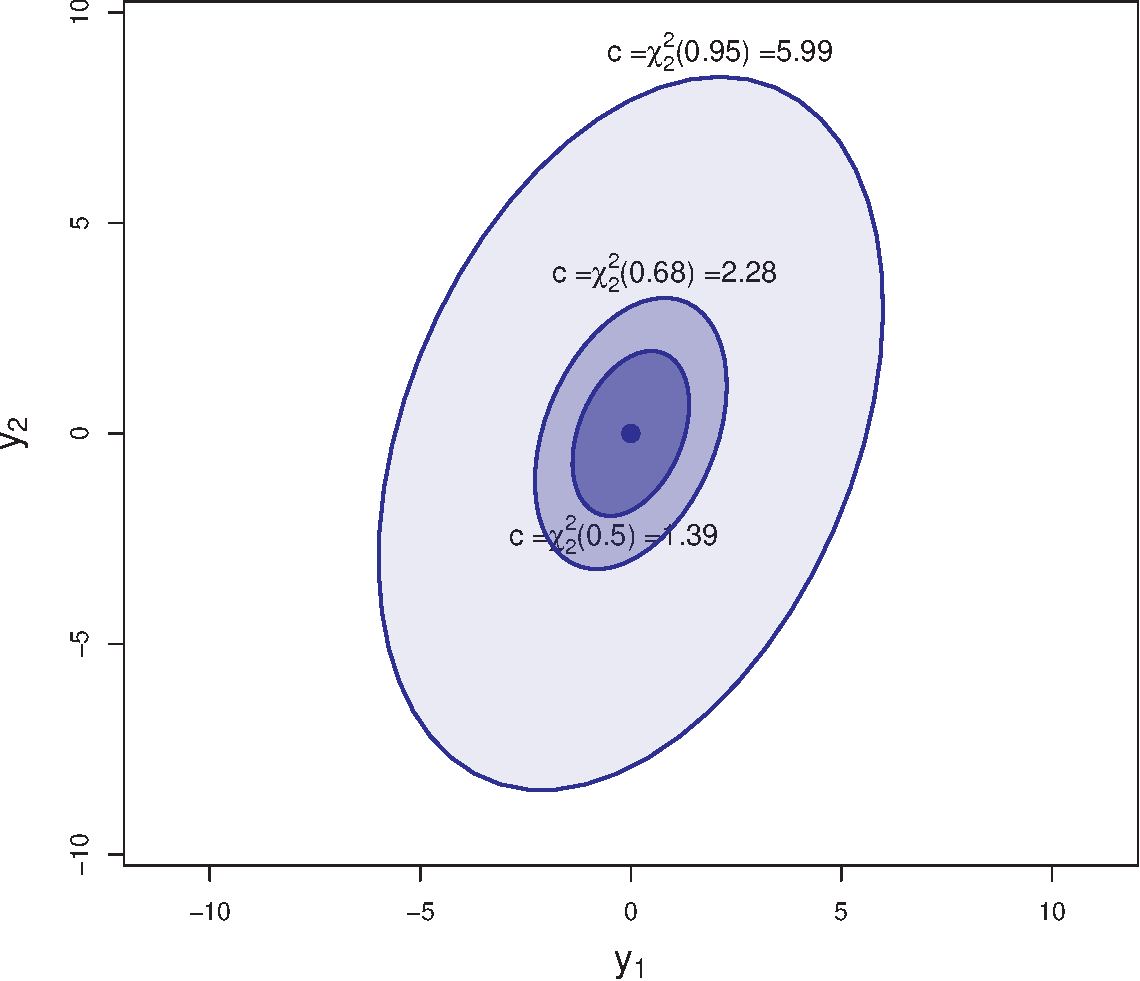
\includegraphics[width=0.7\linewidth,height=\textheight,keepaspectratio]{figs/ch04/fig-ellipses-coverage-1.pdf}

}

\caption{\label{fig-ellipses-coverage}Data ellipses of 50\%, 68\% and
95\% coverage when the means are \(\bar{\mathbf{y}} = \mathbf{0}\) and
the variance-covariance matrix is \(\mathbf{S}\).}

\end{figure}%

As always, graphic details matter. Figure~\ref{fig-ellipses-coverage}
uses \texttt{asp\ =\ 1} so that units in the plot are the same for
\(\mathbf{y}_1\) and \(\mathbf{y}_2\), and we can see the greater
variance for \(\mathbf{y}_2\) as well as the correlation. Facilities of
\texttt{grDevices::plotmath()} are used to provide mathematical
annotations in the plot.

\subsection{Ellipse properties}\label{ellipse-properties}

The essential ideas of correlation and regression and their relation to
ellipses go back to Galton (\citeproc{ref-Galton:1886}{1886}). Galton's
goal was to predict (or explain) how a heritable trait, \(Y\), (e.g.,
height) of children was related to that of their parents, \(X\). He made
a semi-graphic table of the frequencies of 928 observations of the
average height of father and mother versus the height of their child,
shown in Figure~\ref{fig-galton-corr}. (Today, we would put child height
on the \(y\) axis, but Galton was working from the table, so he
organized it with parent height as the rows.) He then drew smoothed
contour lines of equal frequencies and had the wonderful visual insight
that these formed concentric shapes that were tolerably close to
ellipses.

He then calculated summaries, \(\text{Ave}(Y | X)\), and, for symmetry,
\(\text{Ave}(X | Y)\), and plotted these as lines of means on his
diagram. Lo and behold, he had a second visual insight: the lines of
means of (\(Y | X\)) and (\(X | Y\)) corresponded approximately to the
loci of horizontal and vertical tangents to the concentric ellipses. To
complete the picture, he added lines showing the geometric major and
minor axes of the family of ellipses (which turned out to be the
principal components) with the result shown in
Figure~\ref{fig-galton-corr}. \index{principal components}
\index{ellipses}

\begin{figure}[htb!]

\centering{

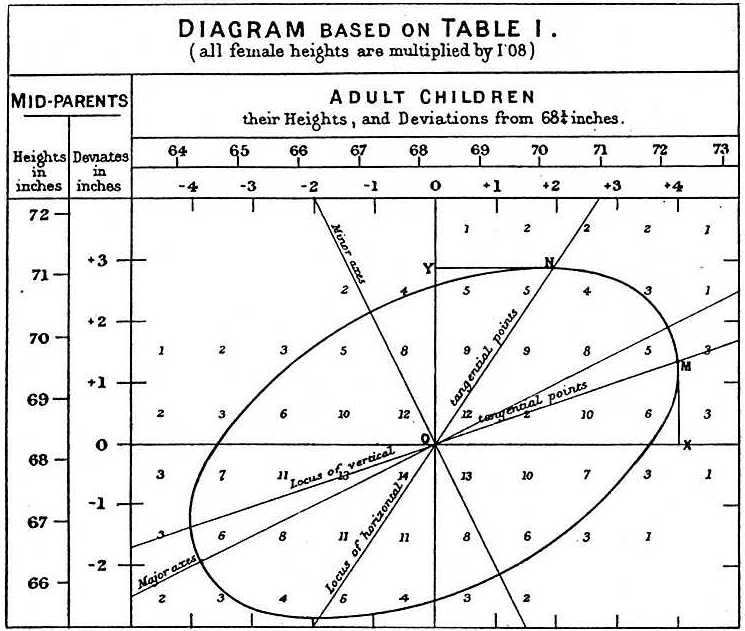
\includegraphics[width=0.7\linewidth,height=\textheight,keepaspectratio]{images/galton-corr.jpg}

}

\caption{\label{fig-galton-corr}Galton's 1886 diagram, showing the
relationship of height of children to the average of their parents'
height. The diagram is essentially an overlay of a geometrical
interpretation on a bivariate grouped frequency distribution, shown as
numbers.}

\end{figure}%

For two variables, \(x\) and \(y\), the remarkable properties of the
data ellipse are illustrated in Figure~\ref{fig-galton-ellipse-r}, a
modern reconstruction of Galton's diagram.

\begin{Shaded}
\begin{Highlighting}[]
\FunctionTok{data}\NormalTok{(Galton, }\AttributeTok{package =} \StringTok{"HistData"}\NormalTok{)}
\FunctionTok{sunflowerplot}\NormalTok{(parent }\SpecialCharTok{\textasciitilde{}}\NormalTok{ child, }\AttributeTok{data=}\NormalTok{Galton, }
      \AttributeTok{xlim=}\FunctionTok{c}\NormalTok{(}\DecValTok{61}\NormalTok{,}\DecValTok{75}\NormalTok{), }
      \AttributeTok{ylim=}\FunctionTok{c}\NormalTok{(}\DecValTok{61}\NormalTok{,}\DecValTok{75}\NormalTok{), }
      \AttributeTok{seg.col=}\StringTok{"black"}\NormalTok{, }
        \AttributeTok{xlab=}\StringTok{"Child height"}\NormalTok{, }
      \AttributeTok{ylab=}\StringTok{"Mid Parent height"}\NormalTok{)}

\NormalTok{y.x }\OtherTok{\textless{}{-}} \FunctionTok{lm}\NormalTok{(parent }\SpecialCharTok{\textasciitilde{}}\NormalTok{ child, }\AttributeTok{data=}\NormalTok{Galton)     }\CommentTok{\# regression of y on x}
\FunctionTok{abline}\NormalTok{(y.x, }\AttributeTok{lwd=}\DecValTok{2}\NormalTok{)}
\NormalTok{x.y }\OtherTok{\textless{}{-}} \FunctionTok{lm}\NormalTok{(child }\SpecialCharTok{\textasciitilde{}}\NormalTok{ parent, }\AttributeTok{data=}\NormalTok{Galton)     }\CommentTok{\# regression of x on y}
\NormalTok{cc }\OtherTok{\textless{}{-}} \FunctionTok{coef}\NormalTok{(x.y)}
\FunctionTok{abline}\NormalTok{(}\SpecialCharTok{{-}}\NormalTok{cc[}\DecValTok{1}\NormalTok{]}\SpecialCharTok{/}\NormalTok{cc[}\DecValTok{2}\NormalTok{], }\DecValTok{1}\SpecialCharTok{/}\NormalTok{cc[}\DecValTok{2}\NormalTok{], }\AttributeTok{lwd=}\DecValTok{2}\NormalTok{, }\AttributeTok{col=}\StringTok{"gray"}\NormalTok{)}

\FunctionTok{with}\NormalTok{(Galton, }
\NormalTok{     car}\SpecialCharTok{::}\FunctionTok{dataEllipse}\NormalTok{(child, parent, }
         \AttributeTok{plot.points=}\ConstantTok{FALSE}\NormalTok{, }
         \AttributeTok{levels=}\FunctionTok{c}\NormalTok{(}\FloatTok{0.40}\NormalTok{, }\FloatTok{0.68}\NormalTok{, }\FloatTok{0.95}\NormalTok{), }
         \AttributeTok{lty=}\DecValTok{1}\SpecialCharTok{:}\DecValTok{3}\NormalTok{)}
\NormalTok{    )}
\end{Highlighting}
\end{Shaded}

\begin{figure}[htb!]

\centering{

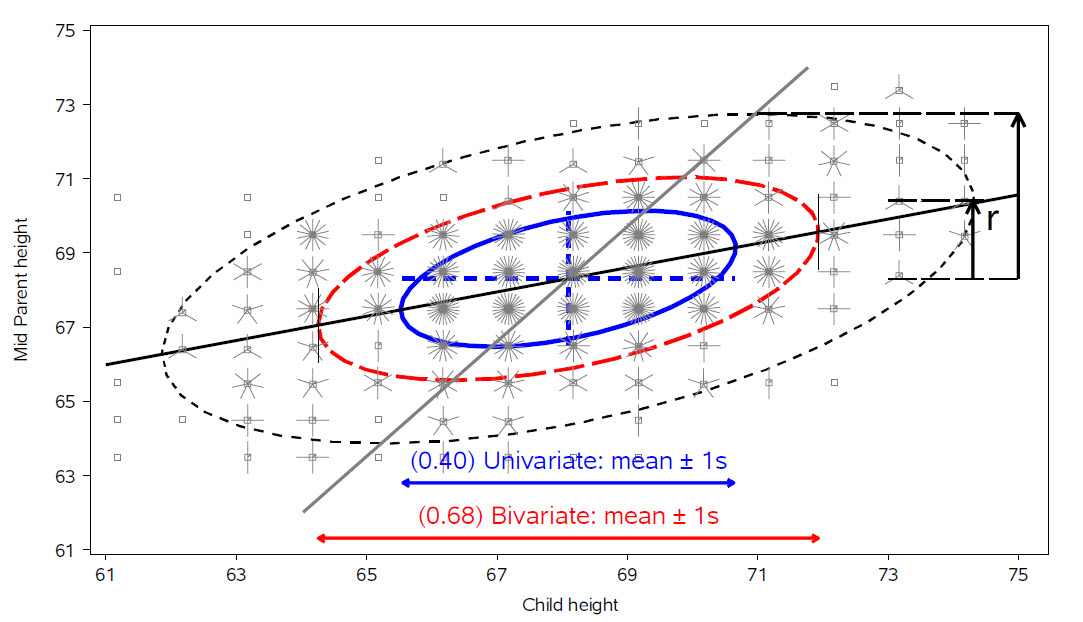
\includegraphics[width=0.8\linewidth,height=\textheight,keepaspectratio]{images/galton-ellipse-r.jpg}

}

\caption{\label{fig-galton-ellipse-r}Sunflower plot of Galton's data on
heights of parents and their children (in.), with 40\%, 68\% and 95\%
data ellipses and the regression lines of \(y\) on \(x\) (black) and
\(x\) on \(y\) (grey).}

\end{figure}%

\begin{itemize}
\item
  The ellipses have the mean vector \((\bar{x}, \bar{y})\) as their
  center.
\item
  The lengths of arms of the \textcolor{blue}{blue} dashed central cross
  show the standard deviations of the variables, which correspond to the
  shadows of the ellipse covering 40\% of the data. These are the
  bivariate analogs of the standard intervals \(\bar{x} \pm 1 s_x\) and
  \(\bar{y} \pm 1 s_y\).
\item
  More generally, shadows (projections) on the coordinate axes, or any
  linear combination of them, give any standard interval,
  \(\bar{x} \pm k s_x\) and \(\bar{y} \pm k s_y\). Those with
  \(k=1, 1.5, 2.45\), have bivariate coverage 40\%, 68\% and 95\%
  respectively, corresponding to these quantiles of the \(\chi^2\)
  distribution with 2 degrees of freedom, i.e.,
  \(\chi^2_2 (.40) \approx 1^2\), \(\chi^2_2 (.68) \approx 1.5^2\), and
  \(\chi^2_2 (.95) \approx 2.45\). The shadows of the 68\% ellipse are
  the bivariate analog of a univariate \(\bar{x} \pm 1 s_x\) interval.
\item
  The regression line predicting \(y\) from \(x\) goes through the
  points where the ellipses have vertical tangents. The \emph{other}
  regression line, predicting \(x\) from \(y\) goes through the points
  of horizontal tangency.
\item
  The correlation \(r(x, y)\) is the ratio of the vertical segment from
  the mean of \(y\) to the regression line to the vertical segment going
  to the top of the ellipse as shown at the right of the figure. It is
  \(r = 0.46\) in this example.
\item
  The residual standard deviation,
  \(s_e = \sqrt{MSE} = \sqrt{\Sigma (y - \bar{y})^2 / n-2}\), is the
  half-length of the ellipse at the mean \(\bar{x}\).
\end{itemize}

Because Galton's values of \texttt{parent} and \texttt{child} height
were recorded in class intervals of 1 in., they are shown as sunflower
symbols in Figure~\ref{fig-galton-ellipse-r}, with multiple `petals'
reflecting the number of observations at each location. This plot
(except for annotations) is constructed using \texttt{sunflowerplot()}
and \texttt{car::dataEllipse()} for the ellipses.

\begin{Shaded}
\begin{Highlighting}[]
\FunctionTok{sunflowerplot}\NormalTok{(parent }\SpecialCharTok{\textasciitilde{}}\NormalTok{ child, }\AttributeTok{data=}\NormalTok{Galton, }
      \AttributeTok{xlim=}\FunctionTok{c}\NormalTok{(}\DecValTok{61}\NormalTok{,}\DecValTok{75}\NormalTok{), }
      \AttributeTok{ylim=}\FunctionTok{c}\NormalTok{(}\DecValTok{61}\NormalTok{,}\DecValTok{75}\NormalTok{), }
      \AttributeTok{seg.col=}\StringTok{"black"}\NormalTok{, }
        \AttributeTok{xlab=}\StringTok{"Child height"}\NormalTok{, }
      \AttributeTok{ylab=}\StringTok{"Mid Parent height"}\NormalTok{)}

\NormalTok{y.x }\OtherTok{\textless{}{-}} \FunctionTok{lm}\NormalTok{(parent }\SpecialCharTok{\textasciitilde{}}\NormalTok{ child, }\AttributeTok{data=}\NormalTok{Galton)    }\CommentTok{\# regression of y on x}
\FunctionTok{abline}\NormalTok{(y.x, }\AttributeTok{lwd=}\DecValTok{2}\NormalTok{)}
\NormalTok{x.y }\OtherTok{\textless{}{-}} \FunctionTok{lm}\NormalTok{(child }\SpecialCharTok{\textasciitilde{}}\NormalTok{ parent, }\AttributeTok{data=}\NormalTok{Galton)    }\CommentTok{\# regression of x on y}
\NormalTok{cc }\OtherTok{\textless{}{-}} \FunctionTok{coef}\NormalTok{(x.y)}
\FunctionTok{abline}\NormalTok{(}\SpecialCharTok{{-}}\NormalTok{cc[}\DecValTok{1}\NormalTok{]}\SpecialCharTok{/}\NormalTok{cc[}\DecValTok{2}\NormalTok{], }\DecValTok{1}\SpecialCharTok{/}\NormalTok{cc[}\DecValTok{2}\NormalTok{], }\AttributeTok{lwd=}\DecValTok{2}\NormalTok{, }\AttributeTok{col=}\StringTok{"gray"}\NormalTok{)}

\FunctionTok{with}\NormalTok{(Galton, }
\NormalTok{     car}\SpecialCharTok{::}\FunctionTok{dataEllipse}\NormalTok{(child, parent, }
         \AttributeTok{plot.points=}\ConstantTok{FALSE}\NormalTok{, }
         \AttributeTok{levels=}\FunctionTok{c}\NormalTok{(}\FloatTok{0.40}\NormalTok{, }\FloatTok{0.68}\NormalTok{, }\FloatTok{0.95}\NormalTok{), }
         \AttributeTok{lty=}\DecValTok{1}\SpecialCharTok{:}\DecValTok{3}\NormalTok{)}
\NormalTok{    )}
\end{Highlighting}
\end{Shaded}

Finally, as Galton noted in his diagram, the principal major and minor
axes of the ellipse have important statistical properties. Pearson
(\citeproc{ref-Pearson:1901}{1901}) would later show that their
directions are determined by the eigenvectors
\(\mathbf{v}_1, \mathbf{v}_2, \dots\) of the covariance matrix
\(\mathbf{S}\) and their radii by the square roots,
\(\sqrt{\lambda_1}, \sqrt{\lambda_2}, \dots\) of the corresponding
eigenvalues.

\subsection{R functions for data
ellipses}\label{r-functions-for-data-ellipses}

A number of packages provide functions for drawing data ellipses in a
scatterplot, with various features.

\begin{itemize}
\tightlist
\item
  \texttt{car::scatterplot()}: uses base R graphics to draw 2D
  scatterplots, with a wide variety of plot enhancements including
  linear and non-parametric smoothers (loess, gam), a formula method,
  e.g., \texttt{y\ \textasciitilde{}\ x\ \textbar{}\ group}, and marking
  points and lines using symbol shape, color, etc. Importantly, the
  \textcolor{brown}{\texttt{\textbf{car}}} %
     \index{car@\texttt{car} package}%
     \index{packages!car@\texttt{car}}%
       package generally allows automatic identification of
  ``noteworthy'' points by their labels in the plot using a variety of
  methods. For example, \texttt{method\ =\ "mahal"} labels cases with
  the most extreme Mahalanobis distances; \texttt{method\ =\ "r"}
  selects points according to their value of \texttt{abs(y)}, which is
  appropriate in residual plots.
\item
  \texttt{car::dataEllipse()}: plots classical or robust data ellipses
  for one or more groups, with the same facilities for point
  identification. The robust version (\texttt{robust=TRUE}) uses the
  multivariate \(t\) distribution (using \texttt{MASS::cov/trob()})
  rather than the Gaussian,
\item
  \texttt{heplots::covEllipses()}: draws classical or robust data
  ellipses for one or more groups in a one-way design and optionally for
  the pooled total sample, where the focus is on homogeneity of
  within-group covariance matrices.
\item
  \texttt{ggplot2::stat\_ellipse()}: uses the calculation methods of
  \texttt{car::dataEllipse()} to add unfilled (\texttt{geom\ =\ "path"})
  or filled (\texttt{geom\ =\ polygon"}) data ellipses in a
  \texttt{ggplot} scatterplot, using inherited aesthetics.
\end{itemize}

\begin{example}[]\protect\hypertarget{exm-prestige}{}\label{exm-prestige}

\textbf{Canadian occupational prestige}

These examples use the data on the prestige of 102 occupational
categories and other measures from the 1971 Canadian Census, recorded in
\texttt{Prestige} \index{Prestige@\texttt{Prestige} data}
\index{datasets!Prestige@\texttt{Prestige}}.\footnote{The dataset was
  collected by Bernard Blishen, William Carroll and Catherine Moore, but
  apparently unpublished. A version updated to the 1981 census is
  described in Blishen et al. (\citeproc{ref-Blishen-etal-1987}{1987}).}
Our interest is in understanding how \texttt{prestige} (the Pineo \&
Porter (\citeproc{ref-PineoPorter2008}{2008}) prestige score for an
occupational category, derived from a social survey) is related to
census measures of the average education, income, percent women of
incumbents in those occupations. Occupation \texttt{type} is a factor
with levels \texttt{"bc"} (blue collar), \texttt{"wc"} (white collar)
and \texttt{"prof"} (professional).

\begin{Shaded}
\begin{Highlighting}[]
\FunctionTok{data}\NormalTok{(Prestige, }\AttributeTok{package=}\StringTok{"carData"}\NormalTok{)}
\CommentTok{\# \textasciigrave{}type\textasciigrave{} is really an ordered factor. Make it so.}
\NormalTok{Prestige}\SpecialCharTok{$}\NormalTok{type }\OtherTok{\textless{}{-}} \FunctionTok{ordered}\NormalTok{(Prestige}\SpecialCharTok{$}\NormalTok{type,}
                         \AttributeTok{levels=}\FunctionTok{c}\NormalTok{(}\StringTok{"bc"}\NormalTok{, }\StringTok{"wc"}\NormalTok{, }\StringTok{"prof"}\NormalTok{))}
\FunctionTok{str}\NormalTok{(Prestige)}
\CommentTok{\# \textquotesingle{}data.frame\textquotesingle{}: 102 obs. of  6 variables:}
\CommentTok{\#  $ education: num  13.1 12.3 12.8 11.4 14.6 ...}
\CommentTok{\#  $ income   : int  12351 25879 9271 8865 8403 11030 8258 14163 11377 11023 ...}
\CommentTok{\#  $ women    : num  11.16 4.02 15.7 9.11 11.68 ...}
\CommentTok{\#  $ prestige : num  68.8 69.1 63.4 56.8 73.5 77.6 72.6 78.1 73.1 68.8 ...}
\CommentTok{\#  $ census   : int  1113 1130 1171 1175 2111 2113 2133 2141 2143 2153 ...}
\CommentTok{\#  $ type     : Ord.factor w/ 3 levels "bc"\textless{}"wc"\textless{}"prof": 3 3 3 3 3 3 3 3 3 3 ...}
\end{Highlighting}
\end{Shaded}

\end{example}

I first illustrate the relation between \texttt{income} and
\texttt{prestige} in Figure~\ref{fig-Prestige-scatterplot-income1} using
\texttt{car::scatterplot()} with many of its bells and whistles,
including marginal boxplots for the variables, the linear regression
line, loess smooth and the 68\% data ellipse.

\begin{Shaded}
\begin{Highlighting}[]
\FunctionTok{scatterplot}\NormalTok{(prestige }\SpecialCharTok{\textasciitilde{}}\NormalTok{ income, }\AttributeTok{data=}\NormalTok{Prestige,}
  \AttributeTok{pch =} \DecValTok{16}\NormalTok{, }\AttributeTok{cex.lab =} \FloatTok{1.25}\NormalTok{,}
  \AttributeTok{regLine =} \FunctionTok{list}\NormalTok{(}\AttributeTok{col =} \StringTok{"red"}\NormalTok{, }\AttributeTok{lwd=}\DecValTok{3}\NormalTok{),}
  \AttributeTok{smooth =} \FunctionTok{list}\NormalTok{(}\AttributeTok{smoother=}\NormalTok{loessLine, }
                \AttributeTok{lty.smooth =} \DecValTok{1}\NormalTok{, }\AttributeTok{lwd.smooth=}\DecValTok{3}\NormalTok{,}
                \AttributeTok{col.smooth =} \StringTok{"darkgreen"}\NormalTok{, }
                \AttributeTok{col.var =} \StringTok{"darkgreen"}\NormalTok{),}
  \AttributeTok{ellipse =} \FunctionTok{list}\NormalTok{(}\AttributeTok{levels =} \FloatTok{0.68}\NormalTok{),}
  \AttributeTok{id =} \FunctionTok{list}\NormalTok{(}\AttributeTok{n=}\DecValTok{4}\NormalTok{, }\AttributeTok{method =} \StringTok{"mahal"}\NormalTok{, }\AttributeTok{col=}\StringTok{"black"}\NormalTok{, }\AttributeTok{cex=}\FloatTok{1.2}\NormalTok{))}
\CommentTok{\# general.managers          lawyers        ministers       physicians }
\CommentTok{\#                2               17               20               24}
\end{Highlighting}
\end{Shaded}

\begin{figure}[htb!]

\centering{

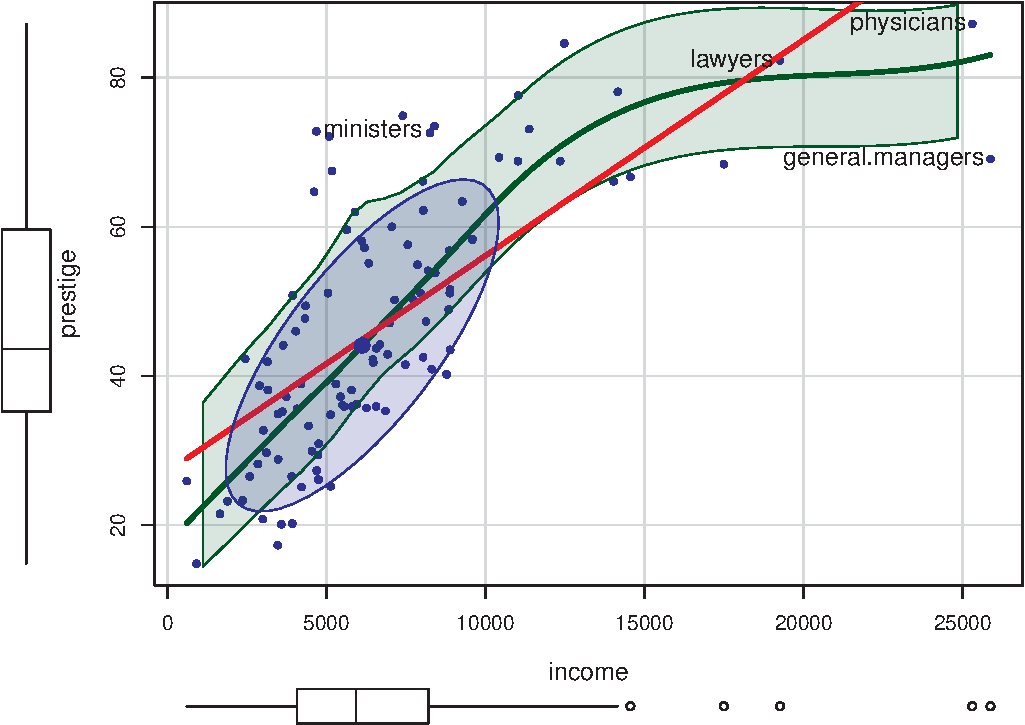
\includegraphics[width=0.7\linewidth,height=\textheight,keepaspectratio]{figs/ch04/fig-Prestige-scatterplot-income1-1.pdf}

}

\caption{\label{fig-Prestige-scatterplot-income1}Scatterplot of prestige
vs.~income, showing the linear regression line (\textcolor{red}{red}),
the loess smooth with a confidence envelope
(\textcolor{darkgreen}{darkgreen}) and a 68\% data ellipse. Points with
the 4 largest Mahalanobis \(D^2\) values are labeled.}

\end{figure}%

There is a lot that can be seen here:

\begin{itemize}
\tightlist
\item
  \texttt{income} is positively skewed, as is often the case.
\item
  The loess smooth, on the scale of income, shows \texttt{prestige}
  increasing up to \$15,000 (these are 1971 incomes), and then leveling
  off.
\item
  The bivariate 1 standard deviation data ellipse, centered at the means
  encloses approximately 68\% of the data points. It adds visual
  information about the correlation and precision of the linear
  regression; but here, the non-linear trend for higher incomes strongly
  suggests a different approach.
\item
  The four points identified by their labels are those with the largest
  Mahalanobis distances. \texttt{scatterplot()} prints their labels to
  the console.
\end{itemize}

Figure~\ref{fig-Prestige-scatterplot-educ1} shows a similar plot for
education, which from the boxplot appears to be reasonably symmetric.
The smoothed curve is quite close to the linear regression, according to
which \texttt{prestige} increases on average
\texttt{coef(lm(prestige\ \textasciitilde{}\ education,\ data=Prestige)){[}"education"{]}}
= 5.361 with each year of education.

\begin{Shaded}
\begin{Highlighting}[]
\FunctionTok{scatterplot}\NormalTok{(prestige }\SpecialCharTok{\textasciitilde{}}\NormalTok{ education, }\AttributeTok{data=}\NormalTok{Prestige,}
  \AttributeTok{pch =} \DecValTok{16}\NormalTok{, }\AttributeTok{cex.lab =} \FloatTok{1.3}\NormalTok{,}
  \AttributeTok{regLine =} \FunctionTok{list}\NormalTok{(}\AttributeTok{col =} \StringTok{"red"}\NormalTok{, }\AttributeTok{lwd=}\DecValTok{3}\NormalTok{),}
  \AttributeTok{smooth =} \FunctionTok{list}\NormalTok{(}\AttributeTok{smoother=}\NormalTok{loessLine, }
                \AttributeTok{lty.smooth =} \DecValTok{1}\NormalTok{, }\AttributeTok{lwd.smooth=}\DecValTok{3}\NormalTok{,}
                \AttributeTok{col.smooth =} \StringTok{"darkgreen"}\NormalTok{, }
                \AttributeTok{col.var =} \StringTok{"darkgreen"}\NormalTok{),}
  \AttributeTok{ellipse =} \FunctionTok{list}\NormalTok{(}\AttributeTok{levels =} \FloatTok{0.68}\NormalTok{),}
  \AttributeTok{id =} \FunctionTok{list}\NormalTok{(}\AttributeTok{n=}\DecValTok{4}\NormalTok{, }\AttributeTok{method =} \StringTok{"mahal"}\NormalTok{, }\AttributeTok{col=}\StringTok{"black"}\NormalTok{, }\AttributeTok{cex=}\FloatTok{1.2}\NormalTok{))}
\CommentTok{\#  physicians file.clerks    newsboys     farmers }
\CommentTok{\#          24          41          53          67}
\end{Highlighting}
\end{Shaded}

\begin{figure}[htb!]

\centering{

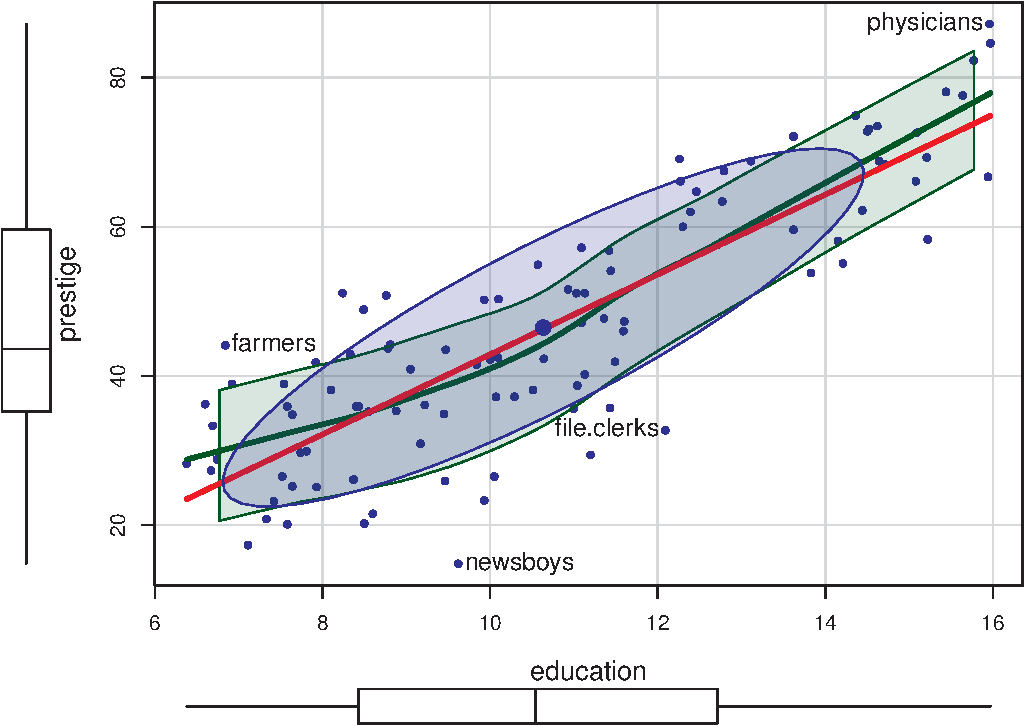
\includegraphics[width=0.7\linewidth,height=\textheight,keepaspectratio]{figs/ch04/fig-Prestige-scatterplot-educ1-1.pdf}

}

\caption{\label{fig-Prestige-scatterplot-educ1}Scatterplot of prestige
vs.~education, showing the linear regression line
(\textcolor{red}{red}), the loess smooth with a confidence envelope
(\textcolor{darkgreen}{darkgreen}) and a 68\% data ellipse.}

\end{figure}%

In this plot, farmers, newsboys, file.clerks and physicians are
identified as noteworthy, for being furthest from the mean by
Mahalanobis distance. In relation to their typical level of education,
these are mostly understandable, but it is nice that farmers are rated
of higher prestige than their level of education would predict.

Note that the \texttt{method} argument for point identification can take
a vector of case numbers indicating the points to be labeled. So, to
label the observations with large absolute standardized residuals in the
linear model \texttt{m}, you can use
\texttt{method\ =\ which(abs(rstandard(m))\ \textgreater{}\ 2)}.

\begin{Shaded}
\begin{Highlighting}[]
\NormalTok{m }\OtherTok{\textless{}{-}} \FunctionTok{lm}\NormalTok{(prestige }\SpecialCharTok{\textasciitilde{}}\NormalTok{ education, }\AttributeTok{data=}\NormalTok{Prestige)}
\FunctionTok{scatterplot}\NormalTok{(prestige }\SpecialCharTok{\textasciitilde{}}\NormalTok{ education, }\AttributeTok{data=}\NormalTok{Prestige,}
    \AttributeTok{pch =} \DecValTok{16}\NormalTok{, }\AttributeTok{cex.lab =} \FloatTok{1.3}\NormalTok{,}
    \AttributeTok{boxplots =} \ConstantTok{FALSE}\NormalTok{,}
    \AttributeTok{regLine =} \FunctionTok{list}\NormalTok{(}\AttributeTok{col =} \StringTok{"red"}\NormalTok{, }\AttributeTok{lwd=}\DecValTok{3}\NormalTok{),}
    \AttributeTok{smooth =} \FunctionTok{list}\NormalTok{(}\AttributeTok{smoother=}\NormalTok{loessLine,}
                  \AttributeTok{lty.smooth =} \DecValTok{1}\NormalTok{, }\AttributeTok{lwd.smooth=}\DecValTok{3}\NormalTok{,}
                  \AttributeTok{col.smooth =} \StringTok{"black"}\NormalTok{, }
                  \AttributeTok{col.var =} \StringTok{"darkgreen"}\NormalTok{),}
    \AttributeTok{ellipse =} \FunctionTok{list}\NormalTok{(}\AttributeTok{levels =} \FloatTok{0.68}\NormalTok{),}
    \AttributeTok{id =} \FunctionTok{list}\NormalTok{(}\AttributeTok{n=}\DecValTok{4}\NormalTok{, }\AttributeTok{method =} \FunctionTok{which}\NormalTok{(}\FunctionTok{abs}\NormalTok{(}\FunctionTok{rstandard}\NormalTok{(m))}\SpecialCharTok{\textgreater{}}\DecValTok{2}\NormalTok{), }
              \AttributeTok{col=}\StringTok{"black"}\NormalTok{, }\AttributeTok{cex=}\FloatTok{1.2}\NormalTok{)) }\SpecialCharTok{|\textgreater{}} 
  \FunctionTok{invisible}\NormalTok{()}
\end{Highlighting}
\end{Shaded}

\begin{figure}[htb!]

\centering{

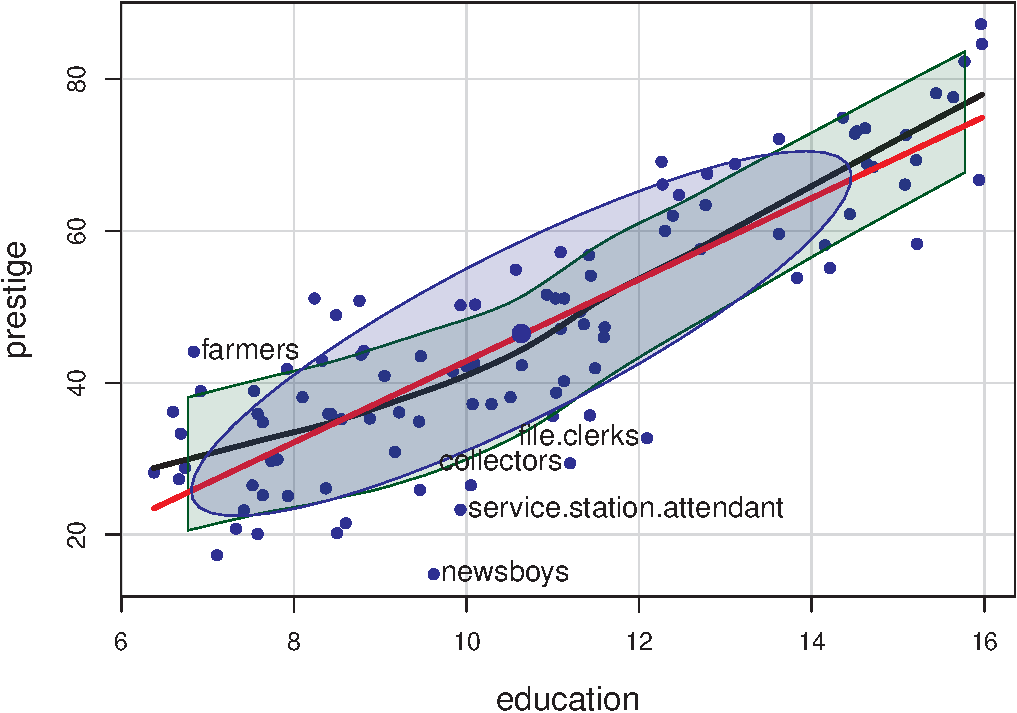
\includegraphics[width=0.7\linewidth,height=\textheight,keepaspectratio]{figs/ch04/fig-Prestige-scatterplot-educ2-1.pdf}

}

\caption{\label{fig-Prestige-scatterplot-educ2}Scatterplot of prestige
vs.~education, labeling points whose absolute standardized residual is
\textgreater{} 2.}

\end{figure}%

\subsection{Handling nonlinearity: Plotting on a log
scale}\label{sec-log-scale}

A typical remedy for the non-linear relationship of income to prestige
is to plot income on a log scale. This usually makes sense, and
expresses a belief that a \textbf{multiple} of or \textbf{percentage
increase} in income has a constant impact on prestige, as opposed to the
\textbf{additive} interpretation for income itself.

For example, the slope of the linear regression line in
Figure~\ref{fig-Prestige-scatterplot-income1} is given by
\texttt{coef(lm(prestige\ \textasciitilde{}\ income,\ data=Prestige)){[}"income"{]}}
= 0.003. Multiplying this by 1000 says that a \$1000 increase in
\texttt{income} is associated with with an average increase of
\texttt{prestige} of 2.9.

In the plot below, \texttt{scatterplot(...,\ log\ =\ "x")} re-scales the
x-axis to the \(\log_e()\) scale. The slope,
\texttt{coef(lm(prestige\ \textasciitilde{}\ log(income),\ data=Prestige)){[}"log(income)"{]}}
= 21.556 says that a 1\% increase in salary is associated with an
average change of 21.55 / 100 in prestige.

\begin{Shaded}
\begin{Highlighting}[]
\FunctionTok{scatterplot}\NormalTok{(prestige }\SpecialCharTok{\textasciitilde{}}\NormalTok{ income, }\AttributeTok{data=}\NormalTok{Prestige,}
  \AttributeTok{log =} \StringTok{"x"}\NormalTok{,}
  \AttributeTok{pch =} \DecValTok{16}\NormalTok{, }\AttributeTok{cex.lab =} \FloatTok{1.3}\NormalTok{,}
  \AttributeTok{regLine =} \FunctionTok{list}\NormalTok{(}\AttributeTok{col =} \StringTok{"red"}\NormalTok{, }\AttributeTok{lwd=}\DecValTok{3}\NormalTok{),}
  \AttributeTok{smooth =} \FunctionTok{list}\NormalTok{(}\AttributeTok{smoother=}\NormalTok{loessLine,}
                \AttributeTok{lty.smooth =} \DecValTok{1}\NormalTok{, }\AttributeTok{lwd.smooth=}\DecValTok{3}\NormalTok{,}
                \AttributeTok{col.smooth =} \StringTok{"darkgreen"}\NormalTok{, }\AttributeTok{col.var =} \StringTok{"darkgreen"}\NormalTok{),}
  \AttributeTok{ellipse =} \FunctionTok{list}\NormalTok{(}\AttributeTok{levels =} \FloatTok{0.68}\NormalTok{),}
  \AttributeTok{id =} \FunctionTok{list}\NormalTok{(}\AttributeTok{n=}\DecValTok{4}\NormalTok{, }\AttributeTok{method =} \StringTok{"mahal"}\NormalTok{, }\AttributeTok{col=}\StringTok{"black"}\NormalTok{, }\AttributeTok{cex=}\FloatTok{1.2}\NormalTok{))}
\CommentTok{\# general.managers        ministers         newsboys      babysitters }
\CommentTok{\#                2               20               53               63}
\end{Highlighting}
\end{Shaded}

\begin{figure}[htb!]

\centering{

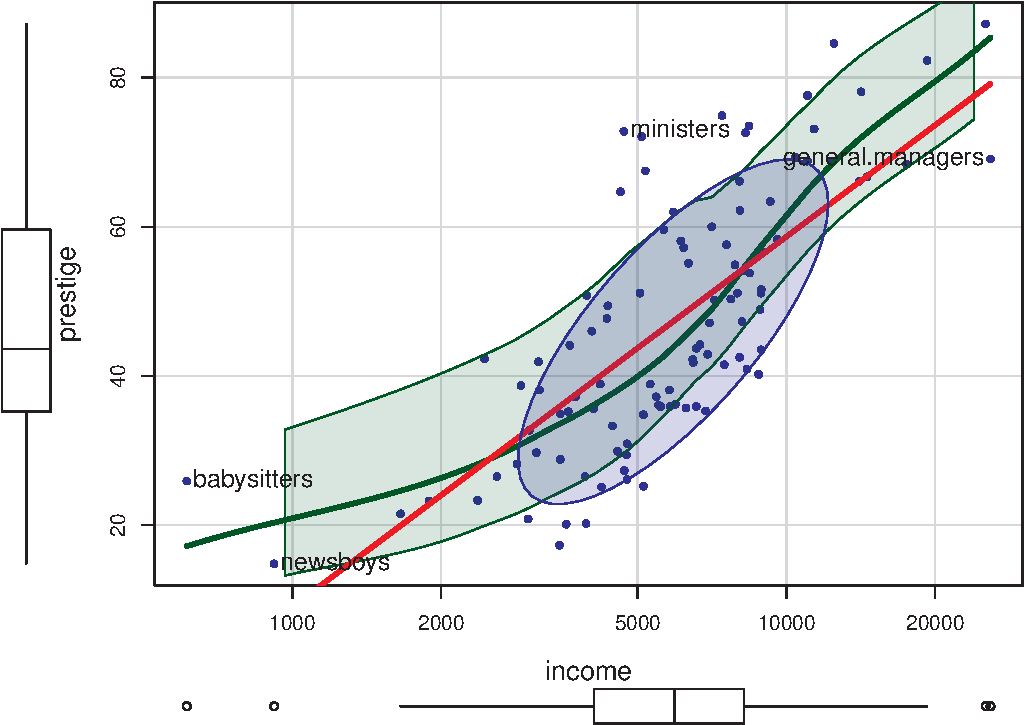
\includegraphics[width=0.7\linewidth,height=\textheight,keepaspectratio]{figs/ch04/fig-Prestige-scatterplot2-1.pdf}

}

\caption{\label{fig-Prestige-scatterplot2}Scatterplot of prestige
vs.~log(income).}

\end{figure}%

The smoothed curve in Figure~\ref{fig-Prestige-scatterplot2} exhibits a
slight tendency to bend upwards, but a linear relation is a reasonable
approximation.

\subsection{Stratifying}\label{sec-stratifying}

\index{stratifier|(}

Before going further, it is instructive to ask what we could see in the
relationship between income and prestige if we stratified by type of
occupation, fitting separate regressions and smooths for blue collar,
white collar and professional incumbents in these occupations.

The formula
\texttt{prestige\ \textasciitilde{}\ income\ \textbar{}\ type} (read:
income \emph{given} type) is a natural way to specify grouping by
\texttt{type}; separate linear regressions and smooths are calculated
for each group, applying the color and point shapes specified by the
\texttt{col} and \texttt{pch} arguments.

\begin{Shaded}
\begin{Highlighting}[]
\FunctionTok{scatterplot}\NormalTok{(prestige }\SpecialCharTok{\textasciitilde{}}\NormalTok{ income }\SpecialCharTok{|}\NormalTok{ type, }\AttributeTok{data=}\NormalTok{Prestige,}
  \AttributeTok{col =} \FunctionTok{c}\NormalTok{(}\StringTok{"blue"}\NormalTok{, }\StringTok{"red"}\NormalTok{, }\StringTok{"darkgreen"}\NormalTok{),}
  \AttributeTok{pch =} \DecValTok{15}\SpecialCharTok{:}\DecValTok{17}\NormalTok{, }\AttributeTok{cex.lab =} \FloatTok{1.3}\NormalTok{,}
  \AttributeTok{grid =} \ConstantTok{FALSE}\NormalTok{,}
  \AttributeTok{legend =} \FunctionTok{list}\NormalTok{(}\AttributeTok{coords=}\StringTok{"bottomright"}\NormalTok{),}
  \AttributeTok{regLine =} \FunctionTok{list}\NormalTok{(}\AttributeTok{lwd=}\DecValTok{3}\NormalTok{, }\AttributeTok{lty =} \StringTok{"longdash"}\NormalTok{),}
  \AttributeTok{smooth=}\FunctionTok{list}\NormalTok{(}\AttributeTok{smoother=}\NormalTok{loessLine, }
              \AttributeTok{var=}\ConstantTok{FALSE}\NormalTok{, }\AttributeTok{lwd.smooth=}\DecValTok{2}\NormalTok{, }\AttributeTok{lty.smooth=}\DecValTok{1}\NormalTok{))}
\end{Highlighting}
\end{Shaded}

\begin{figure}[htb!]

\centering{

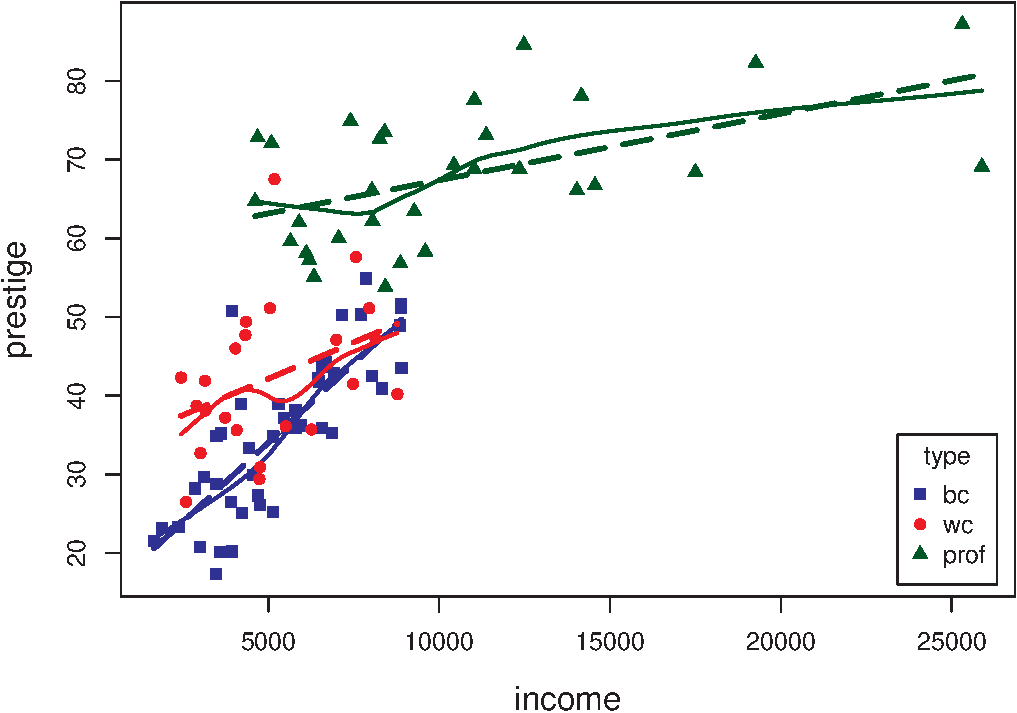
\includegraphics[width=0.7\linewidth,height=\textheight,keepaspectratio]{figs/ch04/fig-Prestige-scatterplot3-1.pdf}

}

\caption{\label{fig-Prestige-scatterplot3}Scatterplot of prestige
vs.~income, stratified by occupational type. This implies a different
interpretation, where occupation type is a moderator variable, so
different regressions apply to each type. The linear regression line is
dashed, while the loess smooth is solid.}

\end{figure}%

This visual analysis offers a different interpretation of the dependence
of prestige on income, which appeared to be non-linear when occupation
type was ignored. Instead, Figure~\ref{fig-Prestige-scatterplot3}
suggests an \emph{interaction} of income by type. In a model formula
this would be expressed as one of:

\begin{Shaded}
\begin{Highlighting}[]
\FunctionTok{lm}\NormalTok{(prestige }\SpecialCharTok{\textasciitilde{}}\NormalTok{ income }\SpecialCharTok{+}\NormalTok{ type }\SpecialCharTok{+}\NormalTok{ income}\SpecialCharTok{:}\NormalTok{type, }\AttributeTok{data =}\NormalTok{ Prestige)}
\FunctionTok{lm}\NormalTok{(prestige }\SpecialCharTok{\textasciitilde{}}\NormalTok{ income }\SpecialCharTok{*}\NormalTok{ type, }\AttributeTok{data =}\NormalTok{ Prestige)}
\end{Highlighting}
\end{Shaded}

These models signify that there are different slopes (and intercepts)
for the three occupational types. In this interpretation, \texttt{type}
is a \textbf{moderator} variable, with a different story. The slopes of
the fitted lines suggest that among blue collar workers, prestige
increases sharply with their income. For white collar and professional
workers, there is still an increasing relation of prestige with income,
but the effect of income (slope) diminishes with higher occupational
category. A different fitted relationship entails a different story.

\index{stratifier|)}

\subsection{Meet the Penguins}\label{sec-penguins}

The \texttt{penguins} dataset from the
\textcolor{brown}{\texttt{\textbf{palmerpenguins}}} package
(\citeproc{ref-R-palmerpenguins}{Horst et al., 2020}) %
   \index{palmerpenguins@\texttt{palmerpenguins} package}%
   \index{packages!palmerpenguins@\texttt{palmerpenguins}}%
     provides further instructive examples of plots and analyses of
multivariate data. The data consists of measurements of body size
(flipper length, body mass, bill length and depth) of 344 penguins
collected at the \href{https://pallter.marine.rutgers.edu/}{Palmer
Research Station} in Antarctica.

\begin{figure}[htb!]

\centering{

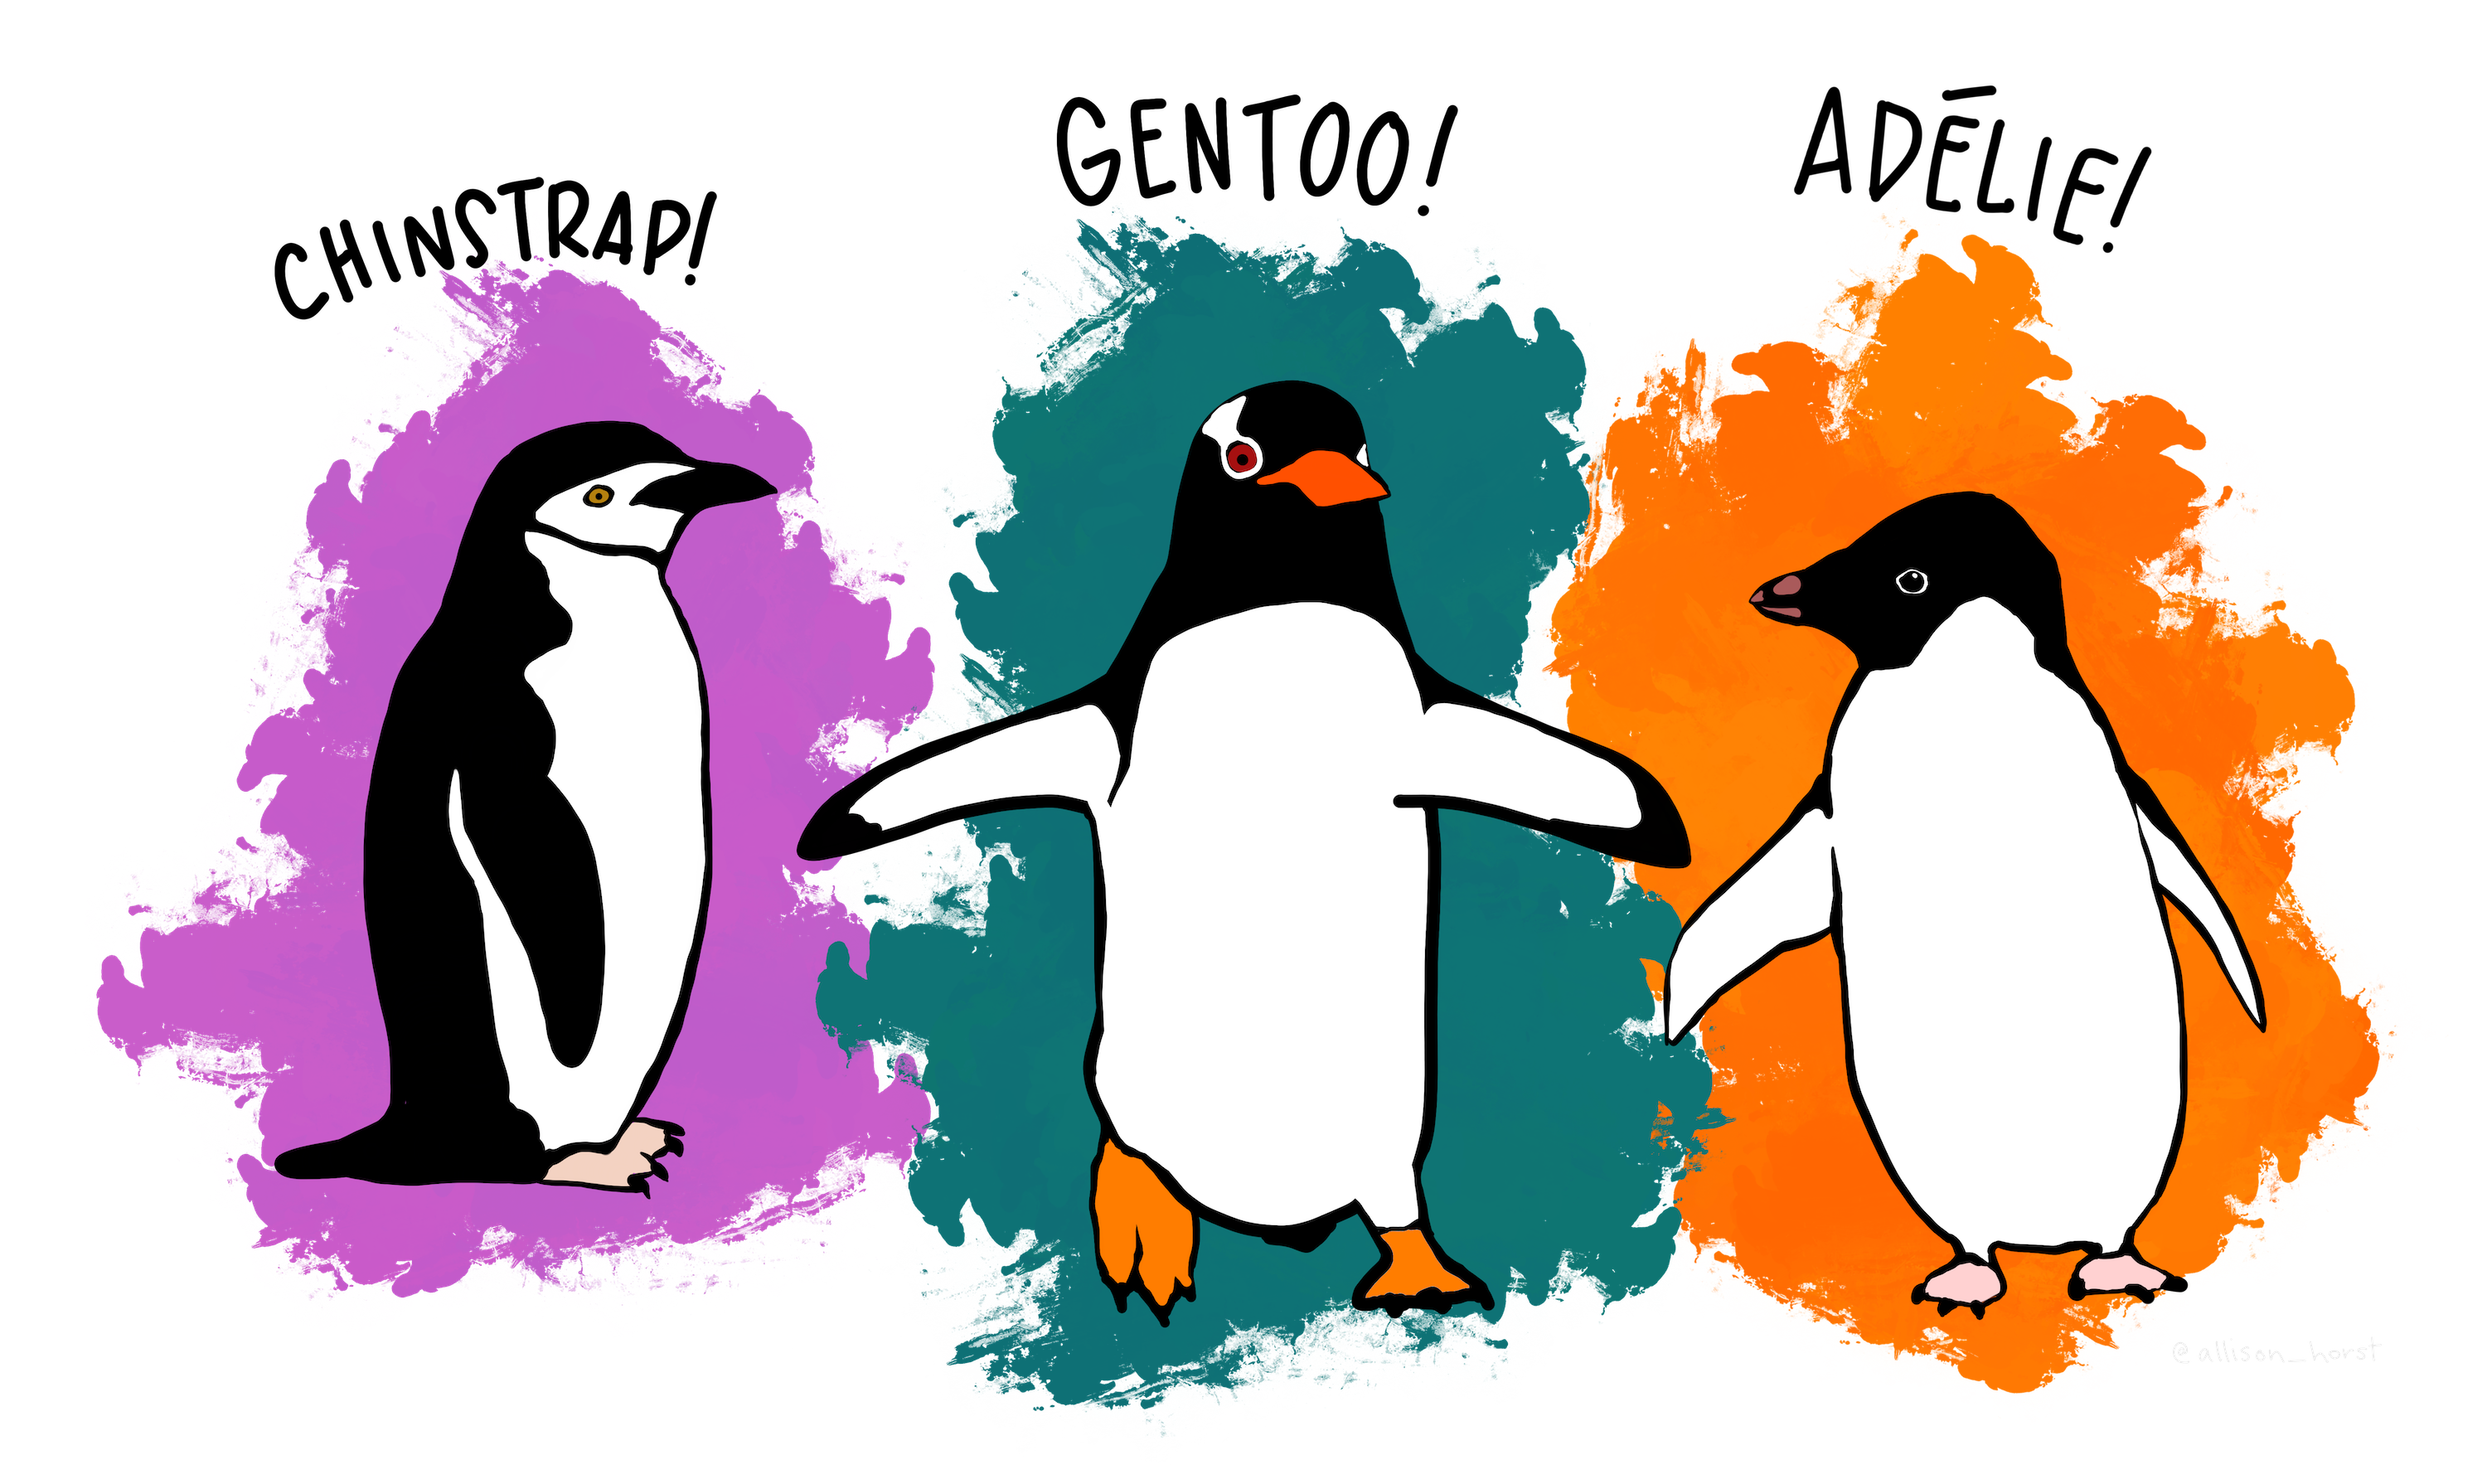
\includegraphics[width=0.5\linewidth,height=\textheight,keepaspectratio]{images/penguins-horst.png}

}

\caption{\label{fig-penguin-species}Penguin species observed in the
Palmer Archipelago. This is a cartoon, but it illustrates some features
of penguin body size measurements, and the colors typically used for
species. Image credit: Allison Horst}

\end{figure}%

There were three different species of penguins (Adélie, Chinstrap \&
Gentoo) collected from 3 islands in the Palmer Archipelago between
2007--2009 (\citeproc{ref-Gorman2014}{Gorman et al., 2014}). The purpose
was to examine differences in size or appearance of these species,
particularly those between the sexes (sexual dimorphism) in relation to
foraging and habitat.

Here, I use a slightly altered version of the dataset,
\texttt{heplots::peng} \index{peng@\texttt{peng} data}
\index{datasets!peng@\texttt{peng}}
\index{heplots@\texttt{heplots} package}
\index{packages!heplots@\texttt{heplots}}, constructed by renaming
variables to remove the units, making factors of character variables and
deleting a few cases with missing data.\footnote{In R 4.5.0, a revised
  version of the \texttt{palmerpenguins} dataset, named
  \texttt{penguins} \index{penguins@\texttt{penguins} data}
  \index{datasets!penguins@\texttt{penguins}} was added to the base R
  \textcolor{brown}{\texttt{\textbf{datasets}}} package %
     \index{datasets@\texttt{datasets} package}%
     \index{packages!datasets@\texttt{datasets}}%
       . This corrected a few of the problems that led me to create
  \texttt{heplots::peng} \index{peng@\texttt{peng} data}
  \index{datasets!peng@\texttt{peng}}
  \index{heplots@\texttt{heplots} package}
  \index{packages!heplots@\texttt{heplots}}, but still retains the cases
  with missing data.}

\begin{Shaded}
\begin{Highlighting}[]
\FunctionTok{data}\NormalTok{(penguins, }\AttributeTok{package =} \StringTok{"palmerpenguins"}\NormalTok{)}
\NormalTok{peng }\OtherTok{\textless{}{-}}\NormalTok{ penguins }\SpecialCharTok{|\textgreater{}}
  \FunctionTok{rename}\NormalTok{(}
    \AttributeTok{bill\_length =}\NormalTok{ bill\_length\_mm, }
    \AttributeTok{bill\_depth =}\NormalTok{ bill\_depth\_mm, }
    \AttributeTok{flipper\_length =}\NormalTok{ flipper\_length\_mm, }
    \AttributeTok{body\_mass =}\NormalTok{ body\_mass\_g}
\NormalTok{  ) }\SpecialCharTok{|\textgreater{}}
  \FunctionTok{mutate}\NormalTok{(}\AttributeTok{species =} \FunctionTok{as.factor}\NormalTok{(species),}
         \AttributeTok{island =} \FunctionTok{as.factor}\NormalTok{(island),}
         \AttributeTok{sex =} \FunctionTok{as.factor}\NormalTok{(}\FunctionTok{substr}\NormalTok{(sex,}\DecValTok{1}\NormalTok{,}\DecValTok{1}\NormalTok{))) }\SpecialCharTok{|\textgreater{}}
\NormalTok{  tidyr}\SpecialCharTok{::}\FunctionTok{drop\_na}\NormalTok{()}

\FunctionTok{glimpse}\NormalTok{(peng)}
\CommentTok{\# Rows: 333}
\CommentTok{\# Columns: 8}
\CommentTok{\# $ species        \textless{}fct\textgreater{} Adelie, Adelie, Adelie, Adelie, Adelie, Ade\textasciitilde{}}
\CommentTok{\# $ island         \textless{}fct\textgreater{} Torgersen, Torgersen, Torgersen, Torgersen,\textasciitilde{}}
\CommentTok{\# $ bill\_length    \textless{}dbl\textgreater{} 39.1, 39.5, 40.3, 36.7, 39.3, 38.9, 39.2, 4\textasciitilde{}}
\CommentTok{\# $ bill\_depth     \textless{}dbl\textgreater{} 18.7, 17.4, 18.0, 19.3, 20.6, 17.8, 19.6, 1\textasciitilde{}}
\CommentTok{\# $ flipper\_length \textless{}int\textgreater{} 181, 186, 195, 193, 190, 181, 195, 182, 191\textasciitilde{}}
\CommentTok{\# $ body\_mass      \textless{}int\textgreater{} 3750, 3800, 3250, 3450, 3650, 3625, 4675, 3\textasciitilde{}}
\CommentTok{\# $ sex            \textless{}fct\textgreater{} m, f, f, f, m, f, m, f, m, m, f, f, m, f, m\textasciitilde{}}
\CommentTok{\# $ year           \textless{}int\textgreater{} 2007, 2007, 2007, 2007, 2007, 2007, 2007, 2\textasciitilde{}}
\end{Highlighting}
\end{Shaded}

There are quite a few variables to choose for illustrating data ellipses
in scatterplots. Here I focus on the measures of their bills,
\texttt{bill\_length} and \texttt{bill\_depth} (indicating curvature)
and show how to use \texttt{ggplot2} for these plots.

I'll be using the penguins data quite a lot, so it is useful to set up
custom colors like those used in Figure~\ref{fig-penguin-species}. My
versions are shown in Figure~\ref{fig-peng-colors} with their color
codes. These are shades of:

\begin{itemize}
\tightlist
\item
  \textcolor{orange}{Adélie}: \textcolor{orange}{orange},
\item
  \textcolor{purple}{Chinstrap}: \textcolor{purple}{purple}, and
\item
  \textcolor{green}{Gentoo}: \textcolor{green}{green}.
\end{itemize}

\begin{figure}[htb!]

\centering{

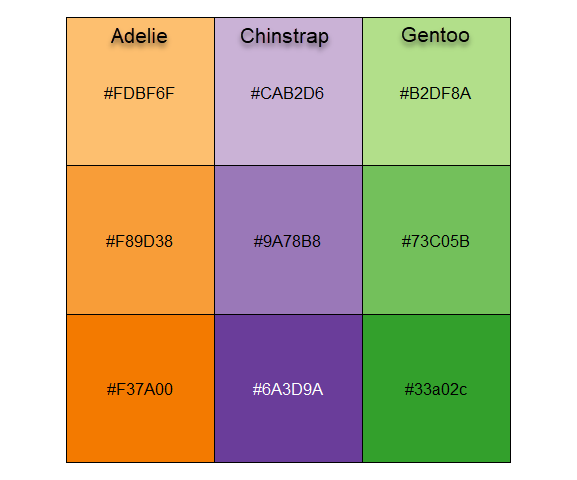
\includegraphics[width=0.5\linewidth,height=\textheight,keepaspectratio]{images/peng-colors.png}

}

\caption{\label{fig-peng-colors}Color palettes used for penguin species.
Each species has a primary hue, which can be used in light, medium or
dark versions.}

\end{figure}%

To use these in \texttt{ggplot2} I define a function
\texttt{peng.colors()} that allows shades of light, medium and dark and
then functions \texttt{scale\_*\_penguins()} for color and fill.

\begin{Shaded}
\begin{Highlighting}[]
\NormalTok{peng.colors }\OtherTok{\textless{}{-}} \ControlFlowTok{function}\NormalTok{(}\AttributeTok{shade=}\FunctionTok{c}\NormalTok{(}\StringTok{"medium"}\NormalTok{, }\StringTok{"light"}\NormalTok{, }\StringTok{"dark"}\NormalTok{)) \{}
\NormalTok{  shade }\OtherTok{=} \FunctionTok{match.arg}\NormalTok{(shade)}
  \CommentTok{\#             light      medium     dark}
\NormalTok{  oranges }\OtherTok{\textless{}{-}} \FunctionTok{c}\NormalTok{(}\StringTok{"\#FDBF6F"}\NormalTok{, }\StringTok{"\#F89D38"}\NormalTok{, }\StringTok{"\#F37A00"}\NormalTok{)  }\CommentTok{\# Adelie}
\NormalTok{  purples }\OtherTok{\textless{}{-}} \FunctionTok{c}\NormalTok{(}\StringTok{"\#CAB2D6"}\NormalTok{, }\StringTok{"\#9A78B8"}\NormalTok{, }\StringTok{"\#6A3D9A"}\NormalTok{)  }\CommentTok{\# Chinstrap}
\NormalTok{  greens }\OtherTok{\textless{}{-}}  \FunctionTok{c}\NormalTok{(}\StringTok{"\#B2DF8A"}\NormalTok{, }\StringTok{"\#73C05B"}\NormalTok{, }\StringTok{"\#33a02c"}\NormalTok{)  }\CommentTok{\# Gentoo}
  
\NormalTok{  cols.vec }\OtherTok{\textless{}{-}} \FunctionTok{c}\NormalTok{(oranges, purples, greens)}
\NormalTok{  cols.mat }\OtherTok{\textless{}{-}} 
    \FunctionTok{matrix}\NormalTok{(cols.vec, }\DecValTok{3}\NormalTok{, }\DecValTok{3}\NormalTok{, }
           \AttributeTok{byrow =} \ConstantTok{TRUE}\NormalTok{,}
           \AttributeTok{dimnames =} \FunctionTok{list}\NormalTok{(}\AttributeTok{species =} \FunctionTok{c}\NormalTok{(}\StringTok{"Adelie"}\NormalTok{, }\StringTok{"Chinstrap"}\NormalTok{, }\StringTok{"Gentoo"}\NormalTok{),}
                           \AttributeTok{shade =} \FunctionTok{c}\NormalTok{(}\StringTok{"light"}\NormalTok{, }\StringTok{"medium"}\NormalTok{, }\StringTok{"dark"}\NormalTok{)))}
  \CommentTok{\# get shaded colors}
\NormalTok{  cols.mat[, shade ]}
\NormalTok{\}}

\CommentTok{\# define color and fill scales}
\NormalTok{scale\_fill\_penguins }\OtherTok{\textless{}{-}} \ControlFlowTok{function}\NormalTok{(}\AttributeTok{shade=}\FunctionTok{c}\NormalTok{(}\StringTok{"medium"}\NormalTok{, }\StringTok{"light"}\NormalTok{, }\StringTok{"dark"}\NormalTok{), ...)\{}
\NormalTok{  shade }\OtherTok{=} \FunctionTok{match.arg}\NormalTok{(shade)}
\NormalTok{  ggplot2}\SpecialCharTok{::}\FunctionTok{discrete\_scale}\NormalTok{(}
    \StringTok{"fill"}\NormalTok{,}\StringTok{"penguins"}\NormalTok{,}
\NormalTok{     scales}\SpecialCharTok{:::}\FunctionTok{manual\_pal}\NormalTok{(}\AttributeTok{values =} \FunctionTok{peng.colors}\NormalTok{(shade)), ...)}
\NormalTok{\}}

\NormalTok{scale\_colour\_penguins }\OtherTok{\textless{}{-}} \ControlFlowTok{function}\NormalTok{(}\AttributeTok{shade=}\FunctionTok{c}\NormalTok{(}\StringTok{"medium"}\NormalTok{, }\StringTok{"light"}\NormalTok{, }\StringTok{"dark"}\NormalTok{), ...)\{}
\NormalTok{  shade }\OtherTok{=} \FunctionTok{match.arg}\NormalTok{(shade)}
\NormalTok{  ggplot2}\SpecialCharTok{::}\FunctionTok{discrete\_scale}\NormalTok{(}
    \StringTok{"colour"}\NormalTok{,}\StringTok{"penguins"}\NormalTok{,}
\NormalTok{    scales}\SpecialCharTok{:::}\FunctionTok{manual\_pal}\NormalTok{(}\AttributeTok{values =} \FunctionTok{peng.colors}\NormalTok{(shade)), ...)}
\NormalTok{\}}
\NormalTok{scale\_color\_penguins }\OtherTok{\textless{}{-}}\NormalTok{ scale\_colour\_penguins}
\end{Highlighting}
\end{Shaded}

This is used to define a \texttt{theme\_penguins()} function that I use
to simply change the color and fill scales for plots below. I also
define a convenience function \texttt{legend\_inside()} to make it less
verbose to position a legend \emph{inside} a plot window, because
outside legends reduce resolution within the plot.

\begin{Shaded}
\begin{Highlighting}[]
\NormalTok{theme\_penguins }\OtherTok{\textless{}{-}} \ControlFlowTok{function}\NormalTok{(}\AttributeTok{shade=}\FunctionTok{c}\NormalTok{(}\StringTok{"medium"}\NormalTok{, }\StringTok{"light"}\NormalTok{, }\StringTok{"dark"}\NormalTok{), }
\NormalTok{                           ...) \{}
\NormalTok{  shade }\OtherTok{=} \FunctionTok{match.arg}\NormalTok{(shade)}
  \FunctionTok{list}\NormalTok{(}\FunctionTok{scale\_color\_penguins}\NormalTok{(}\AttributeTok{shade=}\NormalTok{shade),}
       \FunctionTok{scale\_fill\_penguins}\NormalTok{(}\AttributeTok{shade=}\NormalTok{shade)}
\NormalTok{      )}
\NormalTok{\}}

\NormalTok{legend\_inside }\OtherTok{\textless{}{-}} \ControlFlowTok{function}\NormalTok{(position) \{          }\CommentTok{\# simplify legend placement}
  \FunctionTok{theme}\NormalTok{(}\AttributeTok{legend.position =} \StringTok{"inside"}\NormalTok{,}
        \AttributeTok{legend.position.inside =}\NormalTok{ position)}
\NormalTok{\}}
\end{Highlighting}
\end{Shaded}

An initial plot using \texttt{ggplot2} shown in
Figure~\ref{fig-peng-ggplot1} uses color and point shape to distinguish
the three penguin species. I annotate the plot of points using the
linear regression lines, loess smooths to check for non-linearity and
95\% data ellipses to show precision of the linear relation.

\begin{Shaded}
\begin{Highlighting}[]
\FunctionTok{ggplot}\NormalTok{(peng, }
       \FunctionTok{aes}\NormalTok{(}\AttributeTok{x =}\NormalTok{ bill\_length, }\AttributeTok{y =}\NormalTok{ bill\_depth,}
           \AttributeTok{color =}\NormalTok{ species, }\AttributeTok{shape =}\NormalTok{ species, }\AttributeTok{fill=}\NormalTok{species)) }\SpecialCharTok{+}
  \FunctionTok{geom\_point}\NormalTok{(}\AttributeTok{size=}\DecValTok{2}\NormalTok{) }\SpecialCharTok{+}
  \FunctionTok{geom\_smooth}\NormalTok{(}\AttributeTok{method =} \StringTok{"lm"}\NormalTok{, }\AttributeTok{formula =}\NormalTok{ y }\SpecialCharTok{\textasciitilde{}}\NormalTok{ x,}
              \AttributeTok{se=}\ConstantTok{FALSE}\NormalTok{, }\AttributeTok{linewidth=}\DecValTok{2}\NormalTok{) }\SpecialCharTok{+}
  \FunctionTok{geom\_smooth}\NormalTok{(}\AttributeTok{method =} \StringTok{"loess"}\NormalTok{,  }\AttributeTok{formula =}\NormalTok{ y }\SpecialCharTok{\textasciitilde{}}\NormalTok{ x,}
              \AttributeTok{linewidth =} \FloatTok{1.5}\NormalTok{, }\AttributeTok{se =} \ConstantTok{FALSE}\NormalTok{, }\AttributeTok{alpha=}\FloatTok{0.1}\NormalTok{) }\SpecialCharTok{+}
  \FunctionTok{stat\_ellipse}\NormalTok{(}\AttributeTok{geom =} \StringTok{"polygon"}\NormalTok{, }\AttributeTok{level =} \FloatTok{0.95}\NormalTok{, }\AttributeTok{alpha =} \FloatTok{0.2}\NormalTok{) }\SpecialCharTok{+}
  \FunctionTok{theme\_penguins}\NormalTok{(}\StringTok{"dark"}\NormalTok{) }\SpecialCharTok{+}
  \FunctionTok{legend\_inside}\NormalTok{(}\FunctionTok{c}\NormalTok{(}\FloatTok{0.85}\NormalTok{, }\FloatTok{0.15}\NormalTok{))}
\end{Highlighting}
\end{Shaded}

\begin{figure}[htb!]

\centering{

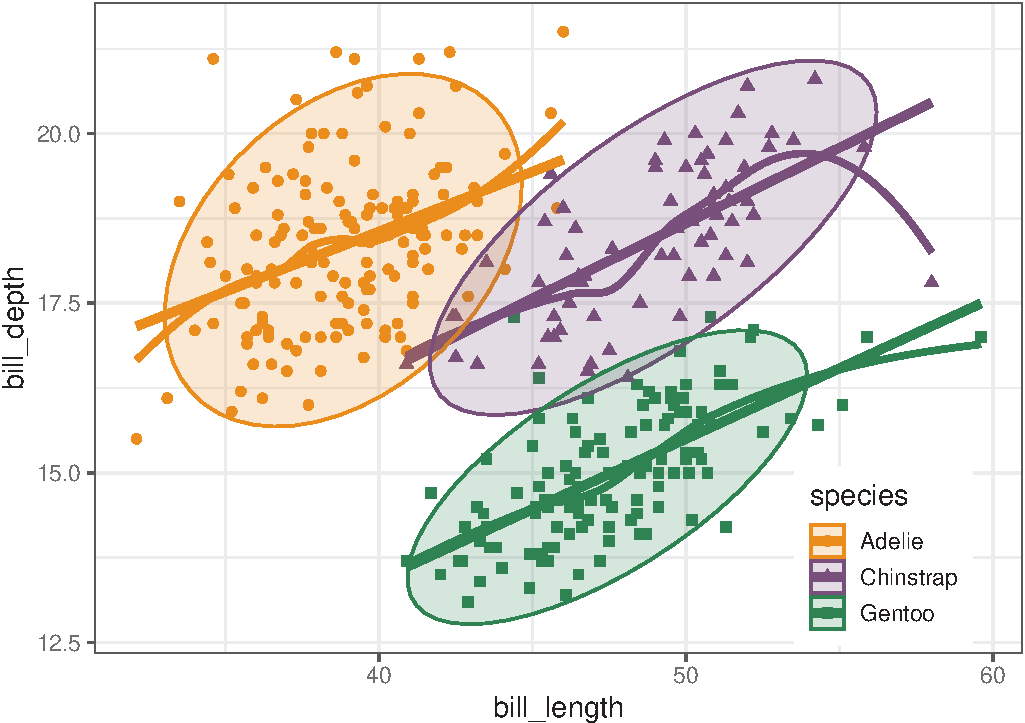
\includegraphics[width=0.7\linewidth,height=\textheight,keepaspectratio]{figs/ch04/fig-peng-ggplot1-1.pdf}

}

\caption{\label{fig-peng-ggplot1}Penguin bill length and bill depth
according to species.}

\end{figure}%

\subsection{Visual thinning}\label{sec-visual-thinning}

\index{visual thinning|(}

Overall, the three species occupy different regions of this 2D space and
for each species the relation between bill length and depth appears
reasonably linear. Given this, we can suppress plotting the data points
to get a visual summary of the data using the fitted regression lines
and data ellipses, as shown in Figure~\ref{fig-peng-ggplot2}.

This idea, of \textbf{visual thinning} a graph to focus on what should
be seen, becomes increasingly useful as the data becomes more complex.
The \texttt{ggplot2} framework encourages this, because we can think of
various components as layers, to be included or not. In
Figure~\ref{fig-peng-ggplot2} I chose to include only the regression
line and add data ellipses of 40\%, 68\% and 95\% coverage to highlight
the increasing bivariate density around the group means.

\begin{Shaded}
\begin{Highlighting}[]
\FunctionTok{ggplot}\NormalTok{(peng, }
       \FunctionTok{aes}\NormalTok{(}\AttributeTok{x =}\NormalTok{ bill\_length, }\AttributeTok{y =}\NormalTok{ bill\_depth,}
           \AttributeTok{color =}\NormalTok{ species, }\AttributeTok{shape =}\NormalTok{ species, }\AttributeTok{fill=}\NormalTok{species)) }\SpecialCharTok{+}
  \FunctionTok{geom\_smooth}\NormalTok{(}\AttributeTok{method =} \StringTok{"lm"}\NormalTok{,  }\AttributeTok{se=}\ConstantTok{FALSE}\NormalTok{, }\AttributeTok{linewidth=}\DecValTok{2}\NormalTok{) }\SpecialCharTok{+}
  \FunctionTok{stat\_ellipse}\NormalTok{(}\AttributeTok{geom =} \StringTok{"polygon"}\NormalTok{, }\AttributeTok{level =} \FloatTok{0.95}\NormalTok{, }\AttributeTok{alpha =} \FloatTok{0.2}\NormalTok{) }\SpecialCharTok{+}
  \FunctionTok{stat\_ellipse}\NormalTok{(}\AttributeTok{geom =} \StringTok{"polygon"}\NormalTok{, }\AttributeTok{level =} \FloatTok{0.68}\NormalTok{, }\AttributeTok{alpha =} \FloatTok{0.2}\NormalTok{) }\SpecialCharTok{+}
  \FunctionTok{stat\_ellipse}\NormalTok{(}\AttributeTok{geom =} \StringTok{"polygon"}\NormalTok{, }\AttributeTok{level =} \FloatTok{0.40}\NormalTok{, }\AttributeTok{alpha =} \FloatTok{0.2}\NormalTok{) }\SpecialCharTok{+}
  \FunctionTok{theme\_penguins}\NormalTok{(}\StringTok{"dark"}\NormalTok{) }\SpecialCharTok{+}
  \FunctionTok{legend\_inside}\NormalTok{(}\FunctionTok{c}\NormalTok{(}\FloatTok{0.85}\NormalTok{, }\FloatTok{0.15}\NormalTok{))}
\end{Highlighting}
\end{Shaded}

\begin{figure}[htb!]

\centering{

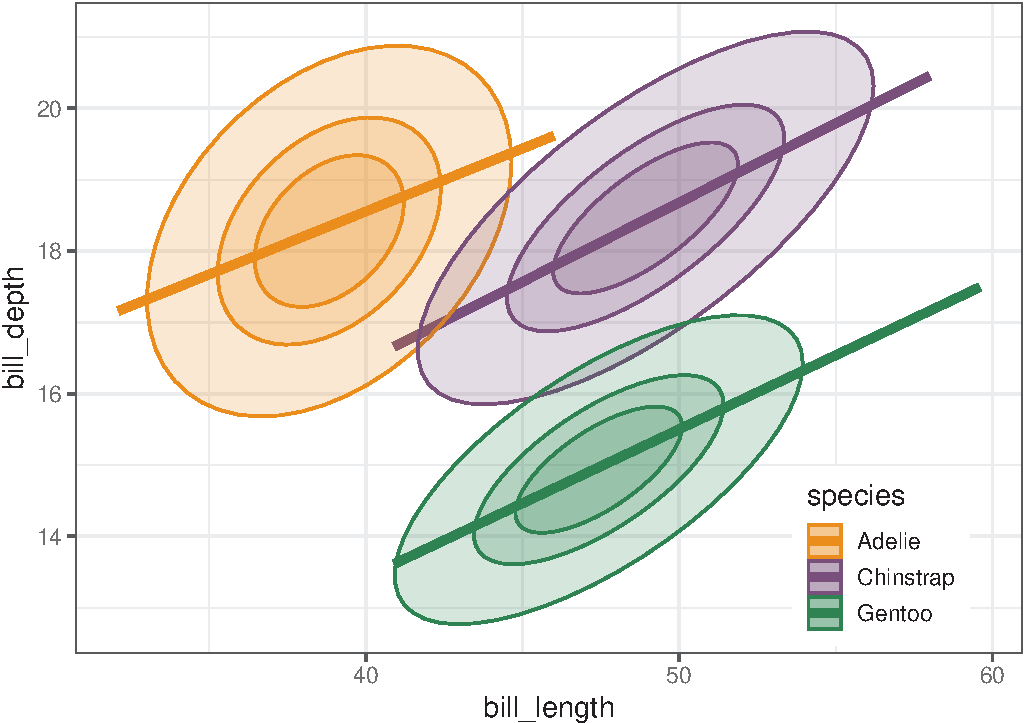
\includegraphics[width=0.7\linewidth,height=\textheight,keepaspectratio]{figs/ch04/fig-peng-ggplot2-1.pdf}

}

\caption{\label{fig-peng-ggplot2}\textbf{Visual thinning}: Suppressing
the data points gives a visual summary of the relation between bill
length and bill depth using the regression line and data ellipses.}

\end{figure}%

\index{data ellipse|)}
\index{visual thinning|)}

\section{Bagplots}\label{sec-bagplots}

\index{bagplot|(}

If you are concerned about the assumption of bivariate normality
entailed by the data ellipse, a very nice non-parametric and robust
alternative is a 2D generalization of a boxplot called a
\textbf{bagplot}, introduced by Peter J. Rousseeuw et al.
(\citeproc{ref-Rousseeuw-etal:2012}{1999}). The idea is very simple. The
bagplot consists of three nested polygons, called the ``bag'', the
``fence'', and the ``loop'':

\begin{itemize}
\item
  \textbf{bag}: The central 50\% box of the boxplot is replaced by a
  polygon called the ``bag'', constructed on the basis of \emph{depth}
  of points from the bivariate depth median point. Depth generalizes the
  univariate concept of rank, but counted from the medians point outward
  in any direction. The bag contains at most 50\% of the most central
  data points. \index{depth}
\item
  \textbf{fence}: The univariate fences are replaced by a ``fence''
  polygon, by expanding the bag outward by a factor (\texttt{coef}),
  usually 3, from the depth median.
\item
  \textbf{loop}: Points beyond the fence (the ``loop'') are potential
  outliers, sometimes plotted as a convex hull surrounding \emph{all} of
  the observations, but better rendered simply as a scatterplot of just
  those points.
\end{itemize}

In this way, the bagplot visualizes the bivariate location (median),
spread, correlation, skewness, and tails of the data. Compared with a
standard data ellipse, it serves as a visual test of normality and
provides a simple way to identify outliers.

Bagplots are implemented in \textcolor{brown}{\texttt{\textbf{gggda}}}
(\citeproc{ref-R-gggda}{Brunson \& Gracey, 2025}) %
   \index{gggda@\texttt{gggda} package}%
   \index{packages!gggda@\texttt{gggda}}%
     in the \texttt{ggplot2} framework as \texttt{geom\_bagplot()} with
computations done via \texttt{stat\_bagplot()}. For the Penguin data,
the bagplot version of Figure~\ref{fig-peng-ggplot2} is shown in
Figure~\ref{fig-peng-bagplot}.

\begin{Shaded}
\begin{Highlighting}[]
\FunctionTok{ggplot}\NormalTok{(peng, }
       \FunctionTok{aes}\NormalTok{(}\AttributeTok{x =}\NormalTok{ bill\_length, }\AttributeTok{y =}\NormalTok{ bill\_depth,}
           \AttributeTok{color =}\NormalTok{ species, }\AttributeTok{shape =}\NormalTok{ species, }\AttributeTok{fill=}\NormalTok{species)) }\SpecialCharTok{+}
  \FunctionTok{geom\_smooth}\NormalTok{(}\AttributeTok{method =} \StringTok{"lm"}\NormalTok{, }\AttributeTok{formula =}\NormalTok{ y }\SpecialCharTok{\textasciitilde{}}\NormalTok{ x,}
              \AttributeTok{se=}\ConstantTok{FALSE}\NormalTok{, }\AttributeTok{linewidth=}\DecValTok{2}\NormalTok{) }\SpecialCharTok{+}
  \FunctionTok{geom\_bagplot}\NormalTok{(}\AttributeTok{bag.alpha =} \FloatTok{0.5}\NormalTok{,}
               \AttributeTok{outlier.size =} \DecValTok{5}\NormalTok{,}
               \AttributeTok{fraction =} \FloatTok{0.5}\NormalTok{,    }\CommentTok{\# bag fraction}
               \AttributeTok{coef =} \FloatTok{2.5}\NormalTok{,        }\CommentTok{\# fence factor}
               \AttributeTok{show.legend =} \ConstantTok{FALSE}\NormalTok{) }\SpecialCharTok{+}
  \FunctionTok{theme\_penguins}\NormalTok{(}\StringTok{"dark"}\NormalTok{) }\SpecialCharTok{+}
  \FunctionTok{legend\_inside}\NormalTok{(}\FunctionTok{c}\NormalTok{(}\FloatTok{0.87}\NormalTok{, }\FloatTok{0.15}\NormalTok{)) }
\end{Highlighting}
\end{Shaded}

\begin{figure}[htb!]

\centering{

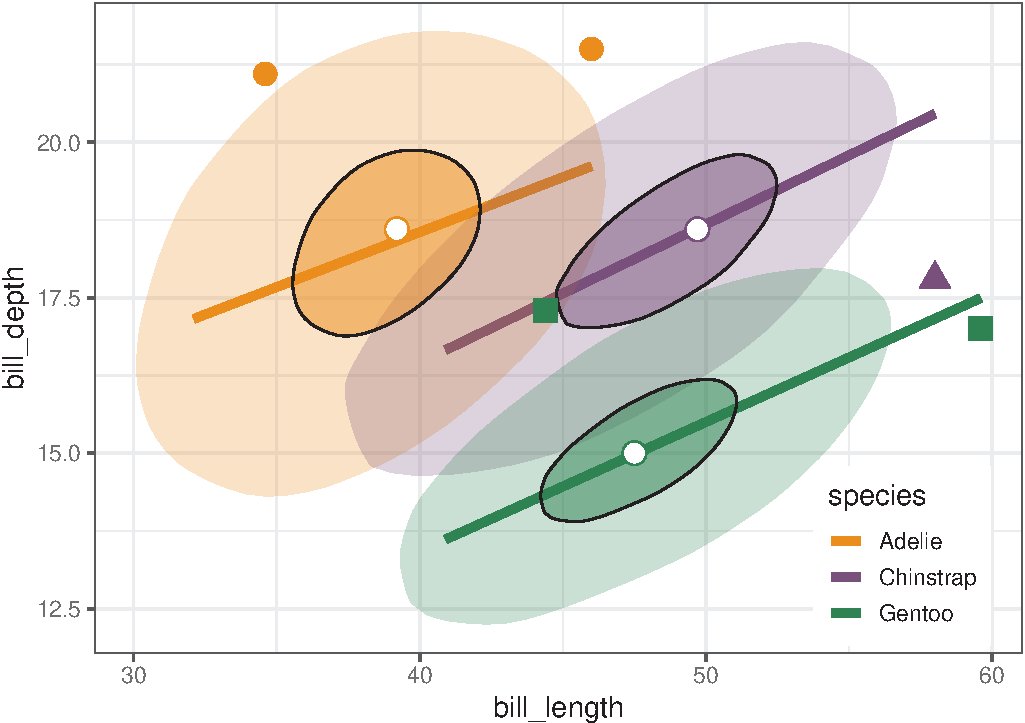
\includegraphics[width=0.7\linewidth,height=\textheight,keepaspectratio]{figs/ch04/fig-peng-bagplot-1.pdf}

}

\caption{\label{fig-peng-bagplot}\textbf{Bagplot}: For each Penguin
species the darker inner (bag) polygon reflects the innermost 50\% of
the data points. The outer (fence) polygon corresponds to points
enclosed by a multiple of the bag. Points outside the fence for each
species are ploted individually.}

\end{figure}%

Compared with the data ellipses shown in Figure~\ref{fig-peng-ggplot2},
the bag polygons have shapes very close to ellipses, giving credence to
the assumption of (approximate) normality. Using the factor
\texttt{coef\ =\ 2.5} causes five points to be flagged as potential
outliers. Bivariate skewness is indicated when the bag and fence is not
symmetric around the central median in some direction, as is slightly
true for all three species.

I discuss other visual tests of multivariate normality in
Section~\ref{sec-multivar-normality} and consider outlier identification
for the Penguin data in Section~\ref{sec-multnorm-penguin} below.
\index{outliers}

\index{bagplot|)}

\section{Non-parametric bivariate density
plots}\label{sec-bivar-density}

\index{non-parametric!bivariate density plot|(}
\index{bivariate density plot|(}

While I emphasize data ellipses (because I like their beautiful
geometry), other visual summaries of the bivariate density are possible
and often useful. To see more detail about the ``shape'' of bivariate
data in a non-parametric way you can use one of the methods described
below to see a model-free representation of your data.

For a single variable, \texttt{stats::density()} and
\texttt{ggplot2::geom\_density()} calculate a smoothed estimate of the
density using nonparametric kernel methods
(\citeproc{ref-Silverman:86}{Silverman, 1986}) whose smoothness is
controlled by a bandwidth parameter, analogous to the span in a loess
smoother. This idea extends to two (and more) variables
(\citeproc{ref-Scott1992}{Scott, 1992}). For bivariate data,
\texttt{MASS::kde2d()} estimates the density on a square \(n \times n\)
grid over the ranges of the variables.

\texttt{ggplot2} provides \texttt{geom\_density\_2d()} which uses
\texttt{MASS::kde2d()} and displays these as contours--- horizontal
slices of the 3D surface at equally-spaced heights and projects these
onto the 2D plane. The \textcolor{brown}{\texttt{\textbf{ggdensity}}}
package (\citeproc{ref-R-ggdensity}{Otto \& Kahle, 2023}) %
   \index{ggdensity@\texttt{ggdensity} package}%
   \index{packages!ggdensity@\texttt{ggdensity}}%
     extends this with \texttt{geom\_hdr()}, computing the high density
regions that bound given levels of probability and maps these to the
\texttt{alpha} transparency aesthetic. A \texttt{method} argument allows
you to specify various nonparametric (\texttt{method\ ="kde"} is the
default) and parametric (\texttt{method\ ="mvnorm"} gives normal data
ellipses) ways to estimate the underlying bivariate distribution.
\index{high density region}

Figure~\ref{fig-peng-ggdensity} shows these side-by-side for comparison.
With \texttt{geom\_density\_2d()} you can specify either the number of
contour \texttt{bins} or the width of these bins (\texttt{binwidth}).
For \texttt{geom\_hdr()}, the \texttt{probs} argument gives a result
that is easier to understand.

\begin{Shaded}
\begin{Highlighting}[]
\FunctionTok{library}\NormalTok{(ggdensity)}
\FunctionTok{library}\NormalTok{(patchwork)}
\NormalTok{p1 }\OtherTok{\textless{}{-}} \FunctionTok{ggplot}\NormalTok{(peng, }
       \FunctionTok{aes}\NormalTok{(}\AttributeTok{x =}\NormalTok{ bill\_length, }\AttributeTok{y =}\NormalTok{ bill\_depth,}
           \AttributeTok{color =}\NormalTok{ species)) }\SpecialCharTok{+}
  \FunctionTok{geom\_smooth}\NormalTok{(}\AttributeTok{method =} \StringTok{"lm"}\NormalTok{,  }\AttributeTok{se=}\ConstantTok{FALSE}\NormalTok{, }\AttributeTok{linewidth=}\DecValTok{2}\NormalTok{) }\SpecialCharTok{+}
  \FunctionTok{geom\_density\_2d}\NormalTok{(}\AttributeTok{linewidth =} \FloatTok{1.1}\NormalTok{, }\AttributeTok{bins =} \DecValTok{8}\NormalTok{) }\SpecialCharTok{+}
  \FunctionTok{ggtitle}\NormalTok{(}\StringTok{"geom\_density\_2d"}\NormalTok{) }\SpecialCharTok{+}
  \FunctionTok{theme\_penguins}\NormalTok{() }\SpecialCharTok{+}
  \FunctionTok{legend\_inside}\NormalTok{(}\FunctionTok{c}\NormalTok{(}\FloatTok{0.85}\NormalTok{, }\FloatTok{0.15}\NormalTok{))}

\NormalTok{p2 }\OtherTok{\textless{}{-}} \FunctionTok{ggplot}\NormalTok{(peng, }
       \FunctionTok{aes}\NormalTok{(}\AttributeTok{x =}\NormalTok{ bill\_length, }\AttributeTok{y =}\NormalTok{ bill\_depth,}
           \AttributeTok{color =}\NormalTok{ species, }\AttributeTok{fill =}\NormalTok{ species)) }\SpecialCharTok{+}
  \FunctionTok{geom\_smooth}\NormalTok{(}\AttributeTok{method =} \StringTok{"lm"}\NormalTok{,  }\AttributeTok{se=}\ConstantTok{FALSE}\NormalTok{, }\AttributeTok{linewidth=}\DecValTok{2}\NormalTok{) }\SpecialCharTok{+}
  \FunctionTok{geom\_hdr}\NormalTok{(}\AttributeTok{probs =} \FunctionTok{c}\NormalTok{(}\FloatTok{0.95}\NormalTok{, }\FloatTok{0.68}\NormalTok{, }\FloatTok{0.4}\NormalTok{), }\AttributeTok{show.legend =} \ConstantTok{FALSE}\NormalTok{) }\SpecialCharTok{+}
  \FunctionTok{ggtitle}\NormalTok{(}\StringTok{"ggdensity::geom\_hdr"}\NormalTok{) }\SpecialCharTok{+}
  \FunctionTok{theme\_penguins}\NormalTok{() }\SpecialCharTok{+}
  \FunctionTok{theme}\NormalTok{(}\AttributeTok{legend.position =} \StringTok{"none"}\NormalTok{)}

\NormalTok{p1 }\SpecialCharTok{+}\NormalTok{ p2}
\end{Highlighting}
\end{Shaded}

\begin{figure}[htb!]

\centering{

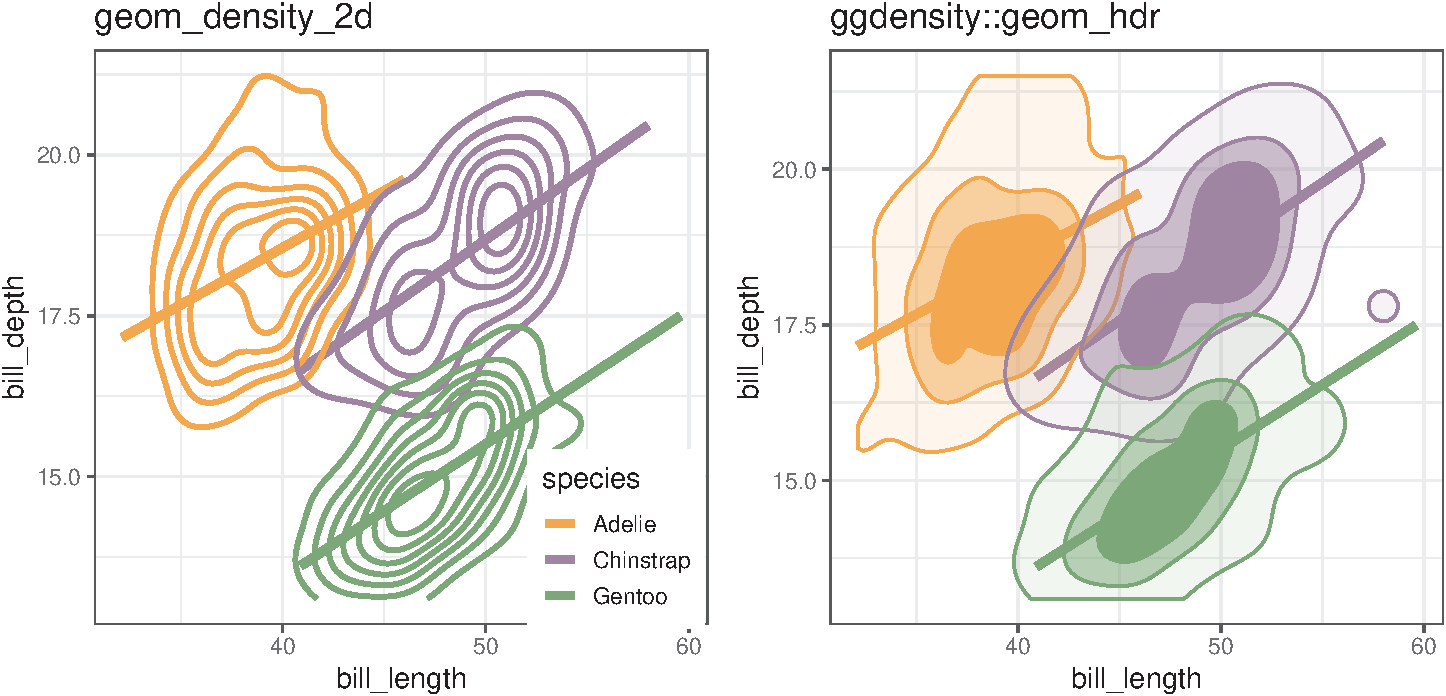
\includegraphics[width=1\linewidth,height=\textheight,keepaspectratio]{figs/ch04/fig-peng-ggdensity-1.pdf}

}

\caption{\label{fig-peng-ggdensity}\textbf{Bivariate densities} show the
contours of the 3D surface representing the frequency in the joint
distribution of bill length and bill depth.}

\end{figure}%

Compared with the data ellipse, which is highly smoothed by the Gaussian
assumption and the bagplot, which is smoothed by the concept of contours
of data depth, the plots in Figure~\ref{fig-peng-ggdensity} show
considerably more detail, and an intriguing suggestion of two peaks for
our Chinstrap penguins. \index{non-parametric!bivariate density plot|)}
\index{bivariate density plot|)}

\section{Simpson's paradox: marginal and conditional
relationships}\label{sec-simpsons}

\index{Simpson's paradox|(}

Because it provides a visual representation of means, variances, and
correlations, the data ellipse is ideally suited as a tool for
illustrating and explicating various phenomena that occur in the
analysis of linear models. One class of simple, but important, examples
concerns the difference between the \emph{marginal relationship} between
variables, ignoring some important factor or covariate, and the
\emph{conditional} relationship, adjusting (controlling) for that
variable.

An important example is \textbf{Simpson's paradox}
(\citeproc{ref-Simpson:51}{Simpson, 1951}) which occurs when the
marginal and conditional relationships differ in direction. That is, the
overall correlation in a model \texttt{y\ \textasciitilde{}\ x} might be
negative, while the within-group correlations in separate models for
each group \texttt{y{[}g{]}\ \textasciitilde{}\ x{[}g{]}} might be
positive, or vice versa. For Flatlanders in 2D space, this is a
puzzlement.

We can see this paradox in the plots of bill length against bill depth
for the penguin data shown in Figure~\ref{fig-peng-simpsons}. Ignoring
penguin species, the marginal, total-sample correlation is slightly
negative as seen in panel (a). The individual-sample ellipses in panel
(b) show that the conditional, within-species correlations are all
positive, with approximately equal regression slopes. However the group
means have a negative relationship, accounting for the negative marginal
correlation when species is ignored.

\begin{figure}[htb!]

\centering{

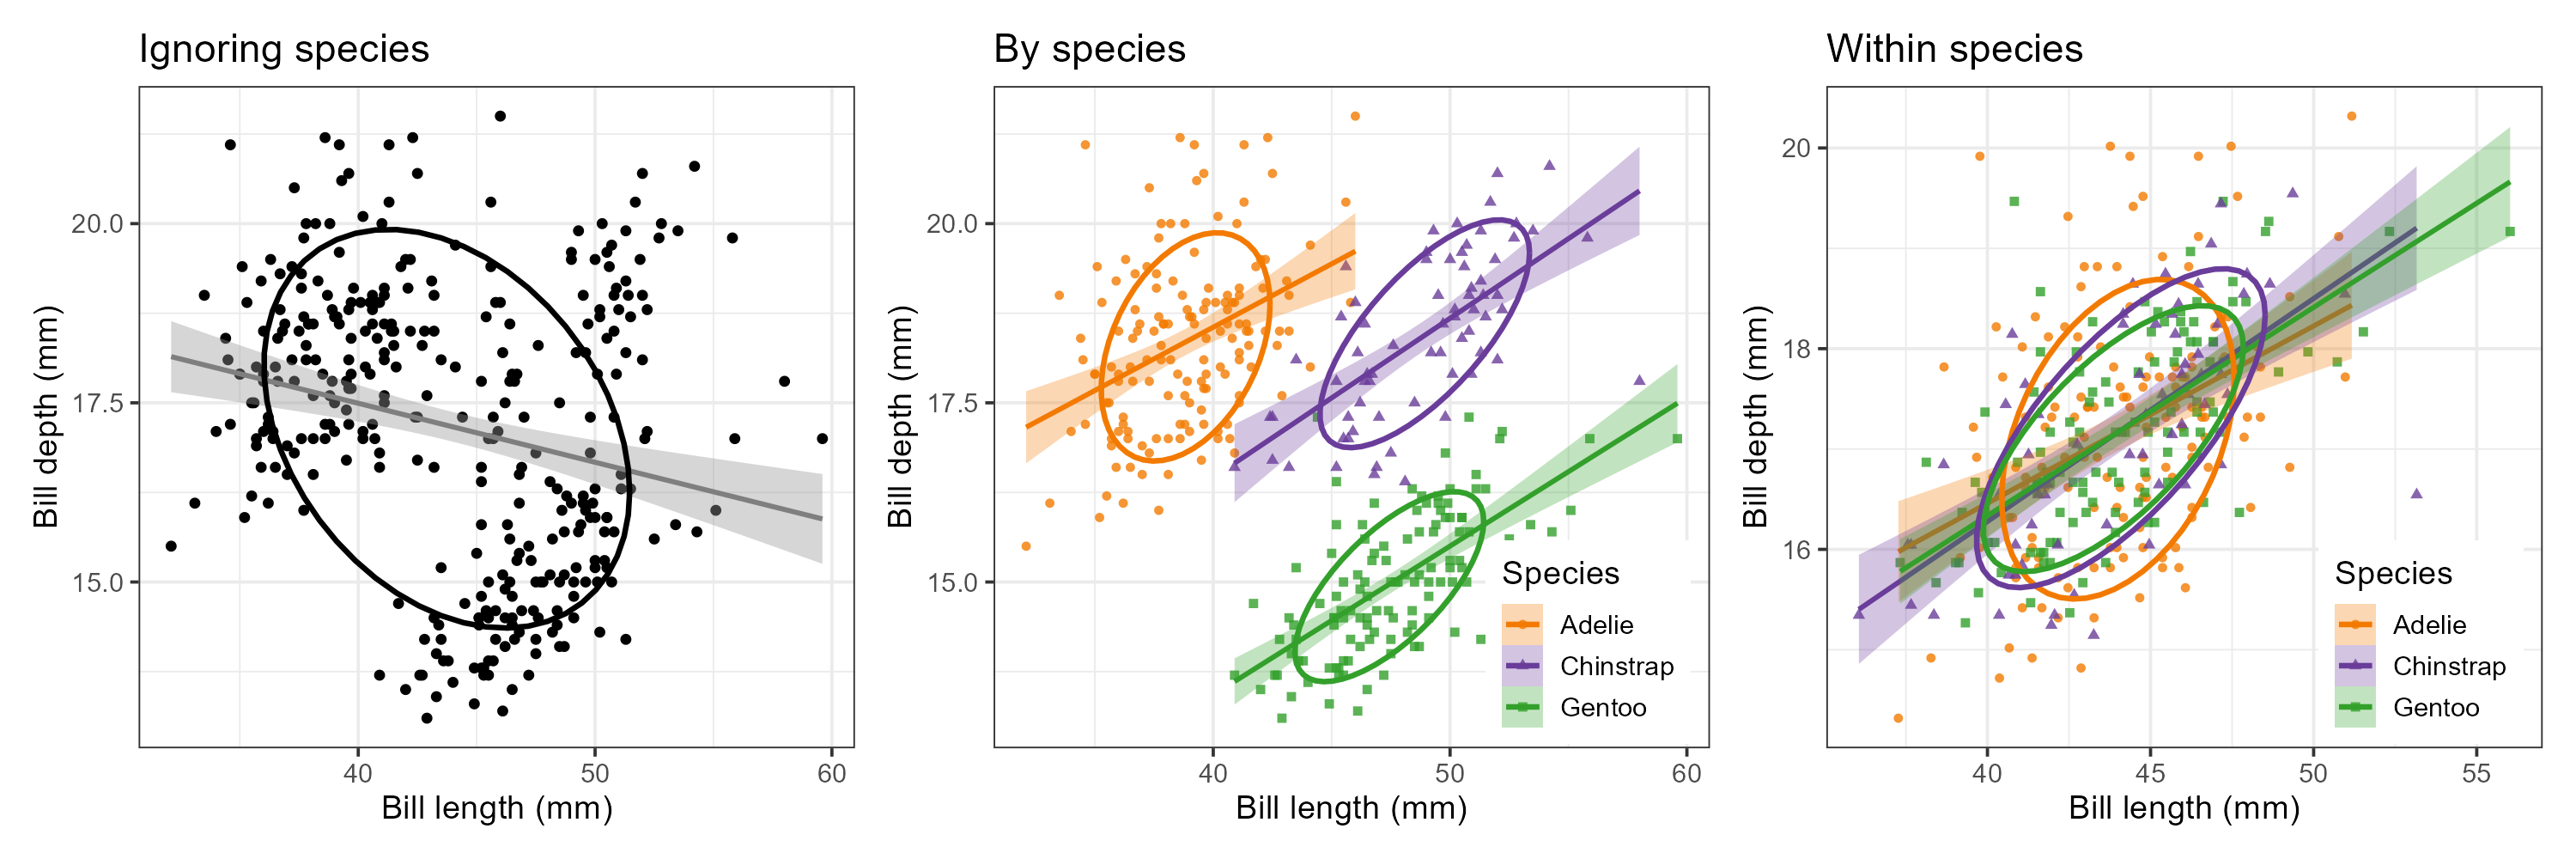
\includegraphics[width=1\linewidth,height=\textheight,keepaspectratio]{images/peng-simpsons.png}

}

\caption{\label{fig-peng-simpsons}Marginal (a), conditional (b), and
pooled within-sample (c) relationships of bill length and depth in the
Penguins data. Each plot shows the 68\% data ellipse and regression
line(s) with 95\% confidence bands.}

\end{figure}%

The regression line in panel (a) is that for the linear model
\texttt{lm(bill\_depth\ \textasciitilde{}\ bill\_length)}, while the
separate lines in panel (b) are those for the model
\texttt{lm(bill\_depth\ \textasciitilde{}\ bill\_length\ *\ species)}
which allows a different slope and intercept for each species.

A correct analysis of the (conditional) relationship between these
variables, controlling or adjusting for mean differences among species,
is based on the pooled within-sample covariance matrix, a weighted
average of the individual within-group \(\mathbf{S}_i\),

\[
\mathbf{S}_{\textrm{within}}  =
\sum_{i=1}^g
(n_i - 1) \mathbf{S}_i \, / \, (N - g)
\:\: ,
\]

where \(N = \sum n_i\). The result is shown in panel (c) of
Figure~\ref{fig-peng-simpsons}.

In this graph, the data for each species were first transformed to
deviations from the species means on both variables and then translated
back to the grand means. You can also see here that the shapes and sizes
of the individual data ellipses are roughly comparable, but perhaps not
identical. This visual idea of centering groups to a common mean will
become important in Chapter~\ref{sec-eqcov} when we want to test the
assumption of equality of error covariances in multivariate models.

The \texttt{ggplot2} code for the panels in this figure are shown below.
Note that for components that will be the same across panels, you can
define elements (e.g., \texttt{labels}, \texttt{theme\_penguins()})
once, and then re-use these across several graphs.

\textbf{TODO} This panel tabset looks fine in HTML but is awkward in PDF

\textbf{TODO}: Decide how to handle the other plots \textbf{(a) Ignoring
species}

\begin{Shaded}
\begin{Highlighting}[]
\NormalTok{labels }\OtherTok{\textless{}{-}} \FunctionTok{labs}\NormalTok{(}
  \AttributeTok{x =} \StringTok{"Bill length (mm)"}\NormalTok{,}
  \AttributeTok{y =} \StringTok{"Bill depth (mm)"}\NormalTok{,}
  \AttributeTok{color =} \StringTok{"Species"}\NormalTok{,}
  \AttributeTok{shape =} \StringTok{"Species"}\NormalTok{,}
  \AttributeTok{fill =} \StringTok{"Species"}\NormalTok{) }

\NormalTok{plt1 }\OtherTok{\textless{}{-}} \FunctionTok{ggplot}\NormalTok{(}\AttributeTok{data =}\NormalTok{ peng,}
               \FunctionTok{aes}\NormalTok{(}\AttributeTok{x =}\NormalTok{ bill\_length,}
                   \AttributeTok{y =}\NormalTok{ bill\_depth)) }\SpecialCharTok{+}
  \FunctionTok{geom\_point}\NormalTok{(}\AttributeTok{size =} \FloatTok{1.5}\NormalTok{) }\SpecialCharTok{+}
  \FunctionTok{geom\_smooth}\NormalTok{(}\AttributeTok{method =} \StringTok{"lm"}\NormalTok{, }\AttributeTok{formula =}\NormalTok{ y }\SpecialCharTok{\textasciitilde{}}\NormalTok{ x, }
              \AttributeTok{se =} \ConstantTok{TRUE}\NormalTok{, }\AttributeTok{color =} \StringTok{"gray50"}\NormalTok{) }\SpecialCharTok{+}
  \FunctionTok{stat\_ellipse}\NormalTok{(}\AttributeTok{level =} \FloatTok{0.68}\NormalTok{, }\AttributeTok{linewidth =} \FloatTok{1.1}\NormalTok{) }\SpecialCharTok{+}
  \FunctionTok{ggtitle}\NormalTok{(}\StringTok{"Ignoring species"}\NormalTok{) }\SpecialCharTok{+}
\NormalTok{  labels}

\NormalTok{plt1}
\end{Highlighting}
\end{Shaded}

\index{Simpson's paradox|)}

\textbf{TODO}: Add stuff on 3D scatterplots, using the
\texttt{R/penguin/peng-3D-rgl.R} example. A start on this is in
\texttt{child/03-3D-scat.qmd}

\section{Multivariate normality and
outliers}\label{sec-multivar-normality}

The relation of the data ellipsoid for \(p\) variables to the
\(\chi^2_p\) distribution with \(p\) degrees of freedom described in
Section~\ref{sec-data-ellipse} is based on the assumption that the data
in \(\mathbf{y}\) is a sample from a multivariate normal distribution
(MVN), with a mean vector \(\boldsymbol{\mu}\) and variance-covariance
matrix \(\boldsymbol{\Sigma}\), so each one implies the other:

\[
\mathbf{y}_{p \times 1} \sim \mathcal{N}(\boldsymbol{\mu}, \boldsymbol{\Sigma}) \Longleftrightarrow D^2_M (\mathbf{y}) \sim \chi^2_p\; .
\]

This fact can be used to assess whether sample data in \(\mathbf{y}\)
does indeed follow a MVN distribution by plotting the
\emph{quantiles}\footnote{The \(p^{th}\)-quantile of a random variable
  \(Y\) is a value, denoted by \(Q_Y(p)\), such that \(X \leq Q_Y(p)\)
  with probability \(p\), i.e., \(\Pr (Y \leq Q_Y(p)) = p\). For
  continuous variables, the quantile is the inverse of the cumulative
  distribution function.} of the \emph{sorted} sample Mahalanobis
\(D^2\) values (denoted \(D^2_{(i)}\)) calculated from
Equation~\ref{eq-Dsq} against the corresponding \(\chi^2_p\) quantiles
found from \texttt{qchisq(df\ =\ p)}. This is called a \(\chi^2\) QQ
plot.

The essential idea is that the plotted points should then approximately
fall along a 45\(^o\) line of slope = 1 when the data are MVN (and axes
are scaled equally). This also provides a simple method to identify
potential outliers as those points which are furthest from the centroid;
that is those for which \(D^2_{(i)}\) is greater than the \(1 - \alpha\)
quantile of \(\chi^2_p\).

The topics of assessing multivariate normality and detecting
multivariate outliers are larger than I consider here. These topics are
also intertwined, because outliers inflate the variance (\(\mathbf{S}\))
of the data, making extreme observations appear less extreme. A variety
of \emph{robust} methods described later
(Section~\ref{sec-robust-estimation}) work by down-weighting outliers,
which is particularly important in assessing whether the residuals from
a multivariate linear model are multivariate normal.

In this section, I focus on the \(\chi^2\) QQ plot and graphical methods
to relate the the points identified as potential outliers to plots in
data space.

\subsection{Galton data}\label{galton-data}

Mahalanobis \(D^2\) values are calculated by
\texttt{heplots::Mahalanobis()}. I illustrate finding the largest
\(D^2_{(i)}\) for the \texttt{Galton} data as shown below. I've used
\(\alpha = 0.01\), giving \(\chi^2_p (0.99) = 9.21\) as an outlier
cutoff, just for the sake of this example. With 928 cases, we would
expect about 1\% or 9 to have larger squared distances than this cutoff.
(Normally, allowing for the fact that we are looking at the largest
values in a sample of size \(n\), we would use a much smaller individual
significance level, say \(\alpha = 0.001\) or smaller still.) Three
cases are identified here.

\begin{Shaded}
\begin{Highlighting}[]
\FunctionTok{data}\NormalTok{(Galton, }\AttributeTok{package =} \StringTok{"HistData"}\NormalTok{)}
\NormalTok{DSQ }\OtherTok{\textless{}{-}} \FunctionTok{Mahalanobis}\NormalTok{(Galton)}
\NormalTok{alpha }\OtherTok{\textless{}{-}} \FloatTok{0.01}
\NormalTok{cutoff }\OtherTok{\textless{}{-}}\NormalTok{ (}\FunctionTok{qchisq}\NormalTok{(}\AttributeTok{p =} \DecValTok{1} \SpecialCharTok{{-}}\NormalTok{ alpha, }\AttributeTok{df =} \FunctionTok{ncol}\NormalTok{(Galton))) }\SpecialCharTok{|\textgreater{}} 
  \FunctionTok{print}\NormalTok{()}
\CommentTok{\# [1] 9.21}
\NormalTok{outliers }\OtherTok{\textless{}{-}} \FunctionTok{which}\NormalTok{(DSQ }\SpecialCharTok{\textgreater{}}\NormalTok{ cutoff) }\SpecialCharTok{|\textgreater{}}
  \FunctionTok{print}\NormalTok{()}
\CommentTok{\# [1]   1  13 897}
\NormalTok{GaltonD }\OtherTok{\textless{}{-}} \FunctionTok{cbind}\NormalTok{(Galton, }\AttributeTok{DSQ =}\NormalTok{ DSQ)}
\NormalTok{GaltonD[outliers,]}
\CommentTok{\#     parent child   DSQ}
\CommentTok{\# 1     70.5  61.7 13.67}
\CommentTok{\# 13    70.5  63.2  9.45}
\CommentTok{\# 897   65.5  72.2  9.49}
\end{Highlighting}
\end{Shaded}

\(\chi^2\) QQ plots are constructed by \texttt{heplots::cqplot()}. For
the Galton data, the result is shown in Figure~\ref{fig-galton-cqplot},
where I've asked for the \texttt{id.n\ =\ 3} with the greatest
\(D^2_{(i)}\) values to be identified with their row numbers in the
plot. The function returns (invisibly) the \(D^2_{(i)}\) and
corresponding \(\chi^2_2\) quantile along with the upper-tail
\(p\)-value.

\begin{Shaded}
\begin{Highlighting}[]
\NormalTok{out }\OtherTok{\textless{}{-}} \FunctionTok{cqplot}\NormalTok{(Galton, }\AttributeTok{id.n =} \DecValTok{3}\NormalTok{)}
\NormalTok{out}
\CommentTok{\#       DSQ quantile        p}
\CommentTok{\# 1   13.67     15.1 0.000539}
\CommentTok{\# 897  9.49     12.9 0.001616}
\CommentTok{\# 13   9.45     11.8 0.002694}
\end{Highlighting}
\end{Shaded}

\begin{figure}[htb!]

\centering{

\includegraphics[width=0.7\linewidth,height=\textheight,keepaspectratio]{figs/ch04/fig-galton-cqplot-1.pdf}

}

\caption{\label{fig-galton-cqplot}Chi-square QQ plot of Galton's data on
heights of parents and their offspring, with a 95\% pointwise confidence
envelope}

\end{figure}%

In the typical use of QQ plots, it essential to have something in the
nature of a confidence band around the points to be able to appreciate
whether, and to what degree the observed data points differ from the
reference distribution. For \texttt{cqplot()}, this helps to assess
whether the data are reasonably distributed as multivariate normal and
also to flag potential outliers.

The pointwise 95\% confidence envelope is calculated as
\(D^2_{(i)} \pm 1.96 \times \text{se} ( D^2_{(i)} )\) where the standard
error is calculated (\citeproc{ref-Chambers-etal:83}{Chambers et al.,
1983, sec. 8.6}) as

\[
 \text{se} ( D^2_{(i)} ) = \frac{\hat{b}}{d ( q_i)} \times \sqrt{  p_i (1-p_i) / n }  \:\: .
\] Here, \(\hat{b}\) is an estimate of the \emph{actual} slope of the
reference line obtained from from the ratio of the interquartile range
of the \(D^2\) values to that of the corresponding \(\chi^2_p\)
distribution. \(d(q_i)\) is the density of the chi square distribution
at the quantile \(q_i\) and \(p_i\) is the corresponding percentile.

So, in Figure~\ref{fig-galton-cqplot}, you can see the same three
points, with largest \(D^2\) identified earlier. The confidence band
shows that uncertainty increases a points get further from the mean, but
by and large, nearly all the points lie within it. The fact that larger
values fall \emph{beneath} the reference line indicates that the sample
\(D^2\) are somewhat \emph{less concentrated} (has a shorter upper tail)
than values in the \(\chi^2_2\) distribution. \index{uncertainty}

To help understand what we are seeing in this example, it is helpful to
view the data in a scatterplot equivalent of
Figure~\ref{fig-galton-ellipse-r}, with the same three observations
labeled and made distinctive in the plot. For this plot, because the
heights are recorded in whole inches, I draw the data ellipses first
without plotting the points and then draw the points using
\texttt{jitter()} on top of the data ellipses.

\begin{Shaded}
\begin{Highlighting}[]
\FunctionTok{set.seed}\NormalTok{(}\DecValTok{47}\NormalTok{)}
\FunctionTok{dataEllipse}\NormalTok{(parent }\SpecialCharTok{\textasciitilde{}}\NormalTok{ child, }\AttributeTok{data =}\NormalTok{ GaltonD,}
            \AttributeTok{levels =} \FunctionTok{c}\NormalTok{(}\FloatTok{0.68}\NormalTok{, }\FloatTok{0.95}\NormalTok{),}
            \AttributeTok{add =} \ConstantTok{FALSE}\NormalTok{, }\AttributeTok{plot.points =} \ConstantTok{FALSE}\NormalTok{,}
            \AttributeTok{center.pch =} \StringTok{"+"}\NormalTok{, }\AttributeTok{center.cex =} \DecValTok{3}\NormalTok{,}
            \AttributeTok{cex.lab =} \FloatTok{1.5}\NormalTok{)}
\FunctionTok{with}\NormalTok{(GaltonD,\{}
  \FunctionTok{points}\NormalTok{(}\FunctionTok{jitter}\NormalTok{(child), }\FunctionTok{jitter}\NormalTok{(parent),}
         \AttributeTok{col =} \FunctionTok{ifelse}\NormalTok{(DSQ }\SpecialCharTok{\textgreater{}}\NormalTok{ cutoff, }\StringTok{"red"}\NormalTok{, }\StringTok{"black"}\NormalTok{),}
         \AttributeTok{pch =} \FunctionTok{ifelse}\NormalTok{(DSQ }\SpecialCharTok{\textgreater{}}\NormalTok{ cutoff, }\DecValTok{16}\NormalTok{, }\DecValTok{1}\NormalTok{),}
         \AttributeTok{cex =} \FunctionTok{ifelse}\NormalTok{(DSQ }\SpecialCharTok{\textgreater{}}\NormalTok{ cutoff, }\DecValTok{2}\NormalTok{, }\FloatTok{0.8}\NormalTok{))}
  \FunctionTok{text}\NormalTok{(child[outliers], parent[outliers], }\AttributeTok{labels =}\NormalTok{ outliers, }\AttributeTok{pos =} \DecValTok{3}\NormalTok{)}
\NormalTok{  \}}
\NormalTok{)}
\end{Highlighting}
\end{Shaded}

\begin{figure}[htb!]

\centering{

\includegraphics[width=0.7\linewidth,height=\textheight,keepaspectratio]{figs/ch04/fig-galton-outliers-1.pdf}

}

\caption{\label{fig-galton-outliers}Scatterplot of Galton's data showing
68\% and 95\% data ellipses for the observations on parent and child
height. The discrete points have been jittered to avoid overplotting.
The three observations identified as having large \(D^2\) values are
labeled with their observation number and given distinctive size, color
and shape.}

\end{figure}%

It is clear from this plot that case 897 is for an exceptionally tall
child of quite short parents, while case 1 and 13 are from very short
children of tall parents; you could call them poster children for
regression toward the mean.

\subsection{Penguin data}\label{sec-multnorm-penguin}

Let's do a similar analysis to assess multivariate normality and
identify possible outliers for the Penguin data. In the
\texttt{cqplot()} shown in Figure~\ref{fig-peng-cqplot}, I use the same
point symbols and colors as in Figure~\ref{fig-peng-ggplot1}. For
illustration, I again label the three most extreme points.

\begin{Shaded}
\begin{Highlighting}[]
\NormalTok{clr }\OtherTok{\textless{}{-}} \FunctionTok{peng.colors}\NormalTok{(}\StringTok{"dark"}\NormalTok{)}
\NormalTok{pch }\OtherTok{\textless{}{-}} \FunctionTok{c}\NormalTok{(}\DecValTok{19}\NormalTok{, }\DecValTok{17}\NormalTok{, }\DecValTok{15}\NormalTok{)   }\CommentTok{\# ggplot symbol defaults for a factor}

\NormalTok{out }\OtherTok{\textless{}{-}} \FunctionTok{cqplot}\NormalTok{(peng[, }\DecValTok{3}\SpecialCharTok{:}\DecValTok{6}\NormalTok{], }
   \AttributeTok{id.n =} \DecValTok{3}\NormalTok{,}
   \AttributeTok{col =}\NormalTok{ clr[peng}\SpecialCharTok{$}\NormalTok{species],}
   \AttributeTok{pch =}\NormalTok{ pch[peng}\SpecialCharTok{$}\NormalTok{species],}
   \AttributeTok{ref.col =} \StringTok{"grey"}\NormalTok{,}
   \AttributeTok{what =} \StringTok{"Penguin numeric variables"}\NormalTok{,}
   \AttributeTok{cex.lab =} \FloatTok{1.25}\NormalTok{)}
\NormalTok{out}
\CommentTok{\#      DSQ quantile       p}
\CommentTok{\# 283 27.8     17.6 0.00150}
\CommentTok{\# 10  13.3     15.1 0.00450}
\CommentTok{\# 35  12.4     13.9 0.00751}
\end{Highlighting}
\end{Shaded}

\begin{figure}[htb!]

\centering{

\includegraphics[width=0.7\linewidth,height=\textheight,keepaspectratio]{figs/ch04/fig-peng-cqplot-1.pdf}

}

\caption{\label{fig-peng-cqplot}Chi-square QQ plot of the Pengiun data.
The three cases with the largest \(D^2\) values are identified with
their case numbers.}

\end{figure}%

One point (case 283) stands out as an extreme multivariate outlier. The
other two (10, 35) are well within the confidence envelope.

To relate this to the data, we can plot the data, as was done in
Figure~\ref{fig-peng-ggplot1}, and label the points identified as
noteworthy. It is a bit tricky to label points selectively in
\texttt{ggplot2} when the criterion for which points to label is
complex, or involves variables outside the data frame. Here, I create a
logical variable \texttt{note}, which is \texttt{TRUE} for the
noteworthy ones. This is then used to subset the data for
\texttt{geom\_text()} that writes the case id numbers.
Figure~\ref{fig-peng-ggplot-out} shows the resulting plot.

\begin{Shaded}
\begin{Highlighting}[]
\NormalTok{DSQ }\OtherTok{\textless{}{-}} \FunctionTok{Mahalanobis}\NormalTok{(peng[, }\DecValTok{3}\SpecialCharTok{:}\DecValTok{6}\NormalTok{])}
\NormalTok{noteworthy }\OtherTok{\textless{}{-}} \FunctionTok{order}\NormalTok{(DSQ, }\AttributeTok{decreasing =} \ConstantTok{TRUE}\NormalTok{)[}\DecValTok{1}\SpecialCharTok{:}\DecValTok{3}\NormalTok{] }\SpecialCharTok{|\textgreater{}} \FunctionTok{print}\NormalTok{()}
\CommentTok{\# [1] 283  10  35}

\NormalTok{peng\_plot }\OtherTok{\textless{}{-}}\NormalTok{ peng }\SpecialCharTok{|\textgreater{}}
\NormalTok{  tibble}\SpecialCharTok{::}\FunctionTok{rownames\_to\_column}\NormalTok{(}\AttributeTok{var =} \StringTok{"id"}\NormalTok{) }\SpecialCharTok{|\textgreater{}} 
  \FunctionTok{mutate}\NormalTok{(}\AttributeTok{note =}\NormalTok{ id }\SpecialCharTok{\%in\%}\NormalTok{ noteworthy)}

\FunctionTok{ggplot}\NormalTok{(peng\_plot, }
       \FunctionTok{aes}\NormalTok{(}\AttributeTok{x =}\NormalTok{ bill\_length, }\AttributeTok{y =}\NormalTok{ bill\_depth,}
           \AttributeTok{color =}\NormalTok{ species, }\AttributeTok{shape =}\NormalTok{ species, }\AttributeTok{fill=}\NormalTok{species)) }\SpecialCharTok{+}
  \FunctionTok{geom\_point}\NormalTok{(}\FunctionTok{aes}\NormalTok{(}\AttributeTok{size=}\NormalTok{note), }\AttributeTok{show.legend =} \ConstantTok{FALSE}\NormalTok{) }\SpecialCharTok{+}
  \FunctionTok{scale\_size\_manual}\NormalTok{(}\AttributeTok{values =} \FunctionTok{c}\NormalTok{(}\FloatTok{1.5}\NormalTok{, }\DecValTok{4}\NormalTok{)) }\SpecialCharTok{+}
  \FunctionTok{geom\_text}\NormalTok{(}\AttributeTok{data =} \FunctionTok{subset}\NormalTok{(peng\_plot, note}\SpecialCharTok{==}\ConstantTok{TRUE}\NormalTok{),}
            \FunctionTok{aes}\NormalTok{(}\AttributeTok{label =}\NormalTok{ id),}
            \AttributeTok{nudge\_y =}\NormalTok{ .}\DecValTok{4}\NormalTok{, }\AttributeTok{color =} \StringTok{"black"}\NormalTok{, }\AttributeTok{size =} \DecValTok{5}\NormalTok{) }\SpecialCharTok{+}
  \FunctionTok{geom\_smooth}\NormalTok{(}\AttributeTok{method =} \StringTok{"lm"}\NormalTok{, }\AttributeTok{formula =}\NormalTok{ y }\SpecialCharTok{\textasciitilde{}}\NormalTok{ x,}
              \AttributeTok{se=}\ConstantTok{FALSE}\NormalTok{, }\AttributeTok{linewidth=}\DecValTok{2}\NormalTok{) }\SpecialCharTok{+}
  \FunctionTok{stat\_ellipse}\NormalTok{(}\AttributeTok{geom =} \StringTok{"polygon"}\NormalTok{, }\AttributeTok{level =} \FloatTok{0.95}\NormalTok{, }\AttributeTok{alpha =} \FloatTok{0.1}\NormalTok{) }\SpecialCharTok{+}
  \FunctionTok{theme\_penguins}\NormalTok{() }\SpecialCharTok{+}
\CommentTok{\#  theme\_bw(base\_size = 14) +}
  \FunctionTok{legend\_inside}\NormalTok{(}\FunctionTok{c}\NormalTok{(}\FloatTok{0.85}\NormalTok{, }\FloatTok{0.15}\NormalTok{)) }
\end{Highlighting}
\end{Shaded}

\begin{figure}[htb!]

\centering{

\includegraphics[width=0.7\linewidth,height=\textheight,keepaspectratio]{figs/ch04/fig-peng-ggplot-out-1.pdf}

}

\caption{\label{fig-peng-ggplot-out}Plot of bill length and bill depth,
with the noteworthy points labeled. Only one (case 283) is a true
multivariate outlier.}

\end{figure}%

Two cases (10, 283) appear to be very unusual in this plot, in relation
to other members of their species. But only case 283 is a true
multivariate outlier, as shown in the cqplot
Figure~\ref{fig-peng-cqplot}. We could call this long-billed penguin
``Cyrano''.\footnote{After the long-nosed Cyrano de Bergerac from Edmund
  Rostand's play. Actually, bird 283 is a female. But, it would be a
  mistake to call her ``Rozanne'' instead.} I'll call case 10, with a
very short and curved bill, ``Hook Nose''.

Of course, we are only looking at the data in the 2D space of the bill
variables, but possible outliers exist in four dimensional Penguin
space. Case 35 is well inside the Adélie ellipse, so perhaps it is
unusual on one of the other variables. It turns out that multivariate
outliers can most often be easily seen as unusual observations in a
projection of the data into the space of the \emph{smallest} principal
components. I return to this example in
Section~\ref{sec-outlier-detection}.

It bears noting that for linear models, multivariate normality is
\textbf{not required} for the response variables or predictors, but
rather is an assumption for the \emph{residuals} from a model. As well,
multivariate outliers in the responses may not turn out to be unusual
when the predictor variables are taken into account. In this example, a
multivariate model would include the effect of \texttt{species},

\begin{Shaded}
\begin{Highlighting}[]
\NormalTok{peng.mod }\OtherTok{\textless{}{-}} \FunctionTok{lm}\NormalTok{(}\FunctionTok{cbind}\NormalTok{(bill\_length, bill\_depth, flipper\_length, body\_mass) }\SpecialCharTok{\textasciitilde{}}\NormalTok{ species, }
               \AttributeTok{data =}\NormalTok{ peng)}
\end{Highlighting}
\end{Shaded}

and there would be cause for concern if the residuals from this model,
\texttt{residuals(peng.mod)} were highly non-normal or showed outliers.

\section{Scatterplot matrices}\label{sec-scatmat}

\index{scatterplot matrix|(}

Going beyond bivariate scatterplots, a \emph{pairs} plot (or
\emph{scatterplot matrix}) displays all possible \(p \times p\) pairs of
\(p\) variables in a matrix-like display where variables \((x_i, x_j)\)
are shown in a plot for row \(i\), column \(j\). This idea, due to
Hartigan (\citeproc{ref-Hartigan:75b}{1975b}), uses small multiple
plots, so that the eye can easily scan across a row or down a column to
see how a given variable is related to all the others.

The most basic version is provided by \texttt{pairs()} in base R. When
one variable is considered as an outcome or response, it is usually
helpful to put this in the first row and column. For the
\texttt{Prestige} data, in addition to income and education, we also
have a measure of \% women in each occupational category.

Plotting these together gives Figure~\ref{fig-prestige-pairs}. In such
plots, the diagonal cells give labels for the variables, but they are
also a guide to interpreting what is shown. In each row, say row 2 for
\texttt{income}, income is the vertical \(y\) variable in plots against
other variables. In each column, say column 3 for \texttt{education},
education is the horizontal \(x\) variable.

\begin{Shaded}
\begin{Highlighting}[]
\FunctionTok{pairs}\NormalTok{(}\SpecialCharTok{\textasciitilde{}}\NormalTok{ prestige }\SpecialCharTok{+}\NormalTok{ income }\SpecialCharTok{+}\NormalTok{ education }\SpecialCharTok{+}\NormalTok{ women,}
      \AttributeTok{data=}\NormalTok{Prestige)}
\end{Highlighting}
\end{Shaded}

\begin{figure}[htb!]

\centering{

\includegraphics[width=0.9\linewidth,height=\textheight,keepaspectratio]{figs/ch04/fig-prestige-pairs-1.pdf}

}

\caption{\label{fig-prestige-pairs}Scatterplot matrix of the variables
in the Prestige dataset produced by \texttt{pairs()}}

\end{figure}%

The plots in the first row show what we have seen before for the
relations between prestige and income and education, adding to those the
plot of prestige vs.~\% women. Plots in the first column show the same
data, but with \(x\) and \(y\) interchanged.

But this basic \texttt{pairs()} plot is very limited. A more
feature-rich version is provided by \texttt{car::scatterplotMatrix()}
which can add the regression lines, loess smooths and data ellipses for
each pair, as shown in Figure~\ref{fig-prestige-spm1}.

The diagonal panels show density curves for the distribution of each
variable; for example, \texttt{education} appears to be multi-modal and
that of \texttt{women} shows that most of the occupations have a low
percentage of women.

The combination of the regression line with the loess smoothed curve,
but without their confidence envelopes, provides about the right amount
of detail to take in at a glance where the relations are non-linear.
We've already seen (Figure~\ref{fig-Prestige-scatterplot-income1}) the
non-linear relation between prestige and income (row 1, column 2) when
occupational type is ignored. But all relations with income in column 2
are non-linear, reinforcing our idea (Section~\ref{sec-log-scale}) that
effects of income should be assessed on a log scale.

\begin{Shaded}
\begin{Highlighting}[]
\FunctionTok{scatterplotMatrix}\NormalTok{(}\SpecialCharTok{\textasciitilde{}}\NormalTok{ prestige }\SpecialCharTok{+}\NormalTok{ income }\SpecialCharTok{+}\NormalTok{ education }\SpecialCharTok{+}\NormalTok{ women,}
  \AttributeTok{data=}\NormalTok{Prestige,}
  \AttributeTok{regLine =} \FunctionTok{list}\NormalTok{(}\AttributeTok{method=}\NormalTok{lm, }\AttributeTok{lty=}\DecValTok{1}\NormalTok{, }\AttributeTok{lwd=}\DecValTok{2}\NormalTok{, }\AttributeTok{col=}\StringTok{"black"}\NormalTok{),}
  \AttributeTok{smooth=}\FunctionTok{list}\NormalTok{(}\AttributeTok{smoother=}\NormalTok{loessLine, }\AttributeTok{spread=}\ConstantTok{FALSE}\NormalTok{,}
              \AttributeTok{lty.smooth=}\DecValTok{1}\NormalTok{, }\AttributeTok{lwd.smooth=}\DecValTok{3}\NormalTok{, }\AttributeTok{col.smooth=}\StringTok{"red"}\NormalTok{),}
  \AttributeTok{ellipse=}\FunctionTok{list}\NormalTok{(}\AttributeTok{levels=}\FloatTok{0.68}\NormalTok{, }\AttributeTok{fill.alpha=}\FloatTok{0.1}\NormalTok{))}
\end{Highlighting}
\end{Shaded}

\begin{figure}[htb!]

\centering{

\includegraphics[width=0.9\linewidth,height=\textheight,keepaspectratio]{figs/ch04/fig-prestige-spm1-1.pdf}

}

\caption{\label{fig-prestige-spm1}Scatterplot matrix of the variables in
the Prestige dataset from \texttt{car::scatterplotMatrix()}.}

\end{figure}%

\texttt{scatterplotMatrix()} can also label points using the
\texttt{id\ =} argument (though this can get messy) and can stratify the
observations by a grouping variable with different symbols and colors.
For example, Figure~\ref{fig-prestige-spm2} uses the syntax
\texttt{\textasciitilde{}\ prestige\ +\ education\ +\ income\ +\ women\ \textbar{}\ type}
to provide separate regression lines, smoothed curves and data ellipses
for the three types of occupations. (The default colors are somewhat
garish, so I use \texttt{scales::hue\_pal()} to mimic the discrete color
scale used in \texttt{ggplot2}).

\begin{Shaded}
\begin{Highlighting}[]
\FunctionTok{scatterplotMatrix}\NormalTok{(}\SpecialCharTok{\textasciitilde{}}\NormalTok{ prestige }\SpecialCharTok{+}\NormalTok{ income }\SpecialCharTok{+}\NormalTok{ education }\SpecialCharTok{+}\NormalTok{ women }\SpecialCharTok{|}\NormalTok{ type,}
  \AttributeTok{data =}\NormalTok{ Prestige,}
  \AttributeTok{col =}\NormalTok{ scales}\SpecialCharTok{::}\FunctionTok{hue\_pal}\NormalTok{()(}\DecValTok{3}\NormalTok{),}
  \AttributeTok{pch =} \DecValTok{15}\SpecialCharTok{:}\DecValTok{17}\NormalTok{,}
  \AttributeTok{smooth=}\FunctionTok{list}\NormalTok{(}\AttributeTok{smoother=}\NormalTok{loessLine, }\AttributeTok{spread=}\ConstantTok{FALSE}\NormalTok{,}
              \AttributeTok{lty.smooth=}\DecValTok{1}\NormalTok{, }\AttributeTok{lwd.smooth=}\DecValTok{3}\NormalTok{, }\AttributeTok{col.smooth=}\StringTok{"black"}\NormalTok{),}
  \AttributeTok{ellipse=}\FunctionTok{list}\NormalTok{(}\AttributeTok{levels=}\FloatTok{0.68}\NormalTok{, }\AttributeTok{fill.alpha=}\FloatTok{0.1}\NormalTok{))}
\end{Highlighting}
\end{Shaded}

\begin{figure}[htb!]

\centering{

\includegraphics[width=0.9\linewidth,height=\textheight,keepaspectratio]{figs/ch04/fig-prestige-spm2-1.pdf}

}

\caption{\label{fig-prestige-spm2}Scatterplot matrix of the variables in
the Prestige dataset from \texttt{car::scatterplotMatrix()}, stratified
by type of occupation.}

\end{figure}%

It is now easy to see why education is multi-modal: blue collar, white
collar and professional occupations have largely non-overlapping years
of education. As well, the distribution of \% women is much higher in
the white collar category.

For the \texttt{penguins} data, given what we've seen before in
Figure~\ref{fig-peng-ggplot1} and Figure~\ref{fig-peng-ggplot2}, we may
wish to suppress details of the points (\texttt{plot.points\ =\ FALSE})
and loess smooths (\texttt{smooth\ =\ FALSE}) to focus attention on the
similarity of regression lines and data ellipses for the three penguin
species. In Figure~\ref{fig-peng-spm}, I've chosen to show boxplots
rather than density curves in the diagonal panels in order to highlight
differences in the means and interquartile ranges of the species, and to
show 68\% and 95\% data ellipses in the off-diagonal panels.

\begin{Shaded}
\begin{Highlighting}[]
\FunctionTok{scatterplotMatrix}\NormalTok{(}\SpecialCharTok{\textasciitilde{}}\NormalTok{ bill\_length }\SpecialCharTok{+}\NormalTok{ bill\_depth }\SpecialCharTok{+}\NormalTok{ flipper\_length }\SpecialCharTok{+}\NormalTok{ body\_mass }\SpecialCharTok{|}\NormalTok{ species,}
  \AttributeTok{data =}\NormalTok{ peng, }
  \AttributeTok{col =} \FunctionTok{peng.colors}\NormalTok{(}\StringTok{"medium"}\NormalTok{), }
  \AttributeTok{legend=}\ConstantTok{FALSE}\NormalTok{,}
  \AttributeTok{ellipse =} \FunctionTok{list}\NormalTok{(}\AttributeTok{levels =} \FunctionTok{c}\NormalTok{(}\FloatTok{0.68}\NormalTok{, }\FloatTok{0.95}\NormalTok{), }
                 \AttributeTok{fill.alpha =} \FloatTok{0.1}\NormalTok{),}
  \AttributeTok{regLine =} \FunctionTok{list}\NormalTok{(}\AttributeTok{lwd=}\DecValTok{3}\NormalTok{),}
  \AttributeTok{diagonal =} \FunctionTok{list}\NormalTok{(}\AttributeTok{method =} \StringTok{"boxplot"}\NormalTok{),}
  \AttributeTok{smooth =} \ConstantTok{FALSE}\NormalTok{,}
  \AttributeTok{plot.points =} \ConstantTok{FALSE}\NormalTok{,}
  \AttributeTok{cex.labels=}\DecValTok{1}\NormalTok{) }
\end{Highlighting}
\end{Shaded}

\begin{figure}[htb!]

\centering{

\includegraphics[width=0.9\linewidth,height=\textheight,keepaspectratio]{figs/ch04/fig-peng-spm-1.pdf}

}

\caption{\label{fig-peng-spm}Scatterplot matrix of the quantitative
variables in the penguins dataset, stratified by species.}

\end{figure}%

It can be seen that the species are widely separated in most of the
bivariate plots. As well, the regression lines for species have similar
slopes and the data ellipses have similar size and shape in most of the
plots. From the boxplots, we can also see that
\textcolor{orange}{Adelie} penguins have shorter bill lengths than the
others, while \textcolor{green}{Gentoo} penguins have smaller bill
depth, but longer flippers and are heavier than
\textcolor{purple}{Chinstrap} and \textcolor{orange}{Adelie} penguins.

\begin{tcolorbox}[enhanced jigsaw, titlerule=0mm, bottomtitle=1mm, left=2mm, opacityback=0, bottomrule=.15mm, breakable, colframe=quarto-callout-note-color-frame, toptitle=1mm, rightrule=.15mm, opacitybacktitle=0.6, colbacktitle=quarto-callout-note-color!10!white, leftrule=.75mm, coltitle=black, arc=.35mm, title=\textcolor{quarto-callout-note-color}{\faInfo}\hspace{0.5em}{Looking ahead}, toprule=.15mm, colback=white]

Figure~\ref{fig-peng-spm} provides a reasonably complete visual summary
of the data in relation to multivariate models that ask ``do the species
differ in their means on these body size measures?'' This corresponds to
the MANOVA model,

\begin{Shaded}
\begin{Highlighting}[]
\NormalTok{peng.mod }\OtherTok{\textless{}{-}} \FunctionTok{lm}\NormalTok{(}\FunctionTok{cbind}\NormalTok{(bill\_length, bill\_depth, flipper\_length, body\_mass) }\SpecialCharTok{\textasciitilde{}}\NormalTok{ species, }
               \AttributeTok{data=}\NormalTok{peng)}
\end{Highlighting}
\end{Shaded}

Hypothesis-error (HE) plots, described in Chapter~\ref{sec-vis-mlm}
provide a better summary of the evidence for the MANOVA test of
differences among means on all variables together. These give an
\(\mathbf{H}\) ellipse reflecting the differences among means, to be
compared with an \(\mathbf{E}\) ellipse reflecting within-group
variation and a visual test of significance.

A related question is ``how well are the penguin species distinguished
by these body size measures?'' Here, the relevant model is linear
discriminant analysis (LDA), where \texttt{species} plays the role of
the response in the model,

\begin{Shaded}
\begin{Highlighting}[]
\NormalTok{peng.lda }\OtherTok{\textless{}{-}}\NormalTok{ MASS}\SpecialCharTok{:}\FunctionTok{lda}\NormalTok{( species }\SpecialCharTok{\textasciitilde{}} \FunctionTok{cbind}\NormalTok{(bill\_length, bill\_depth, flipper\_length, body\_mass), }
               \AttributeTok{data=}\NormalTok{peng)}
\end{Highlighting}
\end{Shaded}

Both MANOVA and LDA depend on the assumption that the variances and
correlations between the variables are the same for all groups. This
assumption can be tested and visualized using the methods in
Chapter~\ref{sec-eqcov}.

\end{tcolorbox}

\subsection{Visual thinning}\label{visual-thinning}

\index{visual thinning|(}

What can you do if there are even more variables than in these examples?
If what you want is a high-level, zoomed-out display summarizing the
pairwise relations more strongly, you can apply the idea of visual
thinning to show only the most important features.

This example uses data on the rate of various crimes in the 50 U.S.
states from the United States Statistical Abstracts, 1970, used by
Hartigan (\citeproc{ref-Hartigan:75}{1975a}) and Friendly
(\citeproc{ref-Friendly:91}{1991}). These are ordered in the dataset
roughly by seriousness of crime or from crimes of violence to property
crimes.

\begin{Shaded}
\begin{Highlighting}[]
\FunctionTok{data}\NormalTok{(crime, }\AttributeTok{package =} \StringTok{"ggbiplot"}\NormalTok{)}
\FunctionTok{str}\NormalTok{(crime)}
\CommentTok{\# \textquotesingle{}data.frame\textquotesingle{}: 50 obs. of  10 variables:}
\CommentTok{\#  $ state   : chr  "Alabama" "Alaska" "Arizona" "Arkansas" ...}
\CommentTok{\#  $ murder  : num  14.2 10.8 9.5 8.8 11.5 6.3 4.2 6 10.2 11.7 ...}
\CommentTok{\#  $ rape    : num  25.2 51.6 34.2 27.6 49.4 42 16.8 24.9 39.6 31.1 ...}
\CommentTok{\#  $ robbery : num  96.8 96.8 138.2 83.2 287 ...}
\CommentTok{\#  $ assault : num  278 284 312 203 358 ...}
\CommentTok{\#  $ burglary: num  1136 1332 2346 973 2139 ...}
\CommentTok{\#  $ larceny : num  1882 3370 4467 1862 3500 ...}
\CommentTok{\#  $ auto    : num  281 753 440 183 664 ...}
\CommentTok{\#  $ st      : chr  "AL" "AK" "AZ" "AR" ...}
\CommentTok{\#  $ region  : Factor w/ 4 levels "Northeast","South",..: 2 4 4 2 4 4 1 2 2 2 ...}
\end{Highlighting}
\end{Shaded}

Figure~\ref{fig-crime-spm} displays the scatterplot matrix for these
seven variables, using only the regression line and data ellipse to show
the linear relation and the loess smooth to show potential
non-linearity. To make this even more schematic, the axis tick marks and
labels are also removed using the \texttt{par()} settings
\texttt{xaxt\ =\ "n",\ yaxt\ =\ "n"}.

\begin{Shaded}
\begin{Highlighting}[]
\NormalTok{crime }\SpecialCharTok{|\textgreater{}}
  \FunctionTok{select}\NormalTok{(}\FunctionTok{where}\NormalTok{(is.numeric)) }\SpecialCharTok{|\textgreater{}}
  \FunctionTok{scatterplotMatrix}\NormalTok{(}
    \AttributeTok{plot.points =} \ConstantTok{FALSE}\NormalTok{,}
    \AttributeTok{ellipse =} \FunctionTok{list}\NormalTok{(}\AttributeTok{levels =} \FloatTok{0.68}\NormalTok{, }\AttributeTok{fill=}\ConstantTok{FALSE}\NormalTok{),}
    \AttributeTok{smooth =} \FunctionTok{list}\NormalTok{(}\AttributeTok{spread =} \ConstantTok{FALSE}\NormalTok{, }
                  \AttributeTok{lwd.smooth=}\DecValTok{2}\NormalTok{, }\AttributeTok{lty.smooth =} \DecValTok{1}\NormalTok{, }
                  \AttributeTok{col.smooth =} \StringTok{"red"}\NormalTok{),}
    \AttributeTok{cex.labels =} \DecValTok{2}\NormalTok{,}
    \AttributeTok{xaxt =} \StringTok{"n"}\NormalTok{, }\AttributeTok{yaxt =} \StringTok{"n"}\NormalTok{)}
\end{Highlighting}
\end{Shaded}

\begin{figure}[htb!]

\centering{

\includegraphics[width=0.9\linewidth,height=\textheight,keepaspectratio]{figs/ch04/fig-crime-spm-1.pdf}

}

\caption{\label{fig-crime-spm}\textbf{Visual thinning}: Scatterplot
matrix of the crime data, showing only high-level summaries of the
linear and nonlinear relations betgween each pair of variables.}

\end{figure}%

We can see that all pairwise correlations are positive, pairs closer to
the main diagonal tend to be more highly correlated and in most cases
the nonparametric smooth doesn't differ much from the linear regression
line. Exceptions to this appear mainly in the columns for
\texttt{robbery} and \texttt{auto} (auto theft).

\index{visual thinning|)}
\index{scatterplot matrix|)}

\section{Corrgrams}\label{sec-corrgram}

\textbf{TODO}: Perhaps split the chapter here

\index{corrgram|(}

What if you want to summarize the data even further simple visual
thinning. For example with many variables you might want to show only
the value of the correlation for each pair of variables, but do so in a
way to help see patterns in the correlations that would be invisible in
just a table.

A \textbf{corrgram} (\citeproc{ref-Friendly:02:corrgram}{Friendly,
2002}) is a visual display of a correlation matrix, where the
correlation can be rendered in a variety of ways to show the direction
and magnitude: circular ``pac-man'' (or pie) symbols, ellipses, colored
vars or shaded rectangles, as shown in
Figure~\ref{fig-corrgram-renderings}.

Another aspect is that of \textbf{effect ordering}
(\citeproc{ref-FriendlyKwan:03:effect}{Friendly \& Kwan, 2003}),
ordering the levels of factors and variables in graphic displays to make
important features most apparent. For variables, this means that we can
arrange the variables in a matrix-like display in such a way as to make
the pattern of relationships easiest to see. Methods to achieve this
include using principal components and cluster analysis to put the most
related variables together as described in Chapter~\ref{sec-pca-biplot}.

\begin{figure}[htb!]

\centering{

\includegraphics[width=0.8\linewidth,height=\textheight,keepaspectratio]{images/corrgram-renderings.png}

}

\caption{\label{fig-corrgram-renderings}\textbf{Corrgrams}: Some
renderings for the value of a correlation in a corrgram display,
conveying sign and magnitude in different ways.}

\end{figure}%

In R, these diagrams can be created using the
\textcolor{brown}{\texttt{\textbf{corrgram}}}
(\citeproc{ref-R-corrgram}{Wright, 2021}) %
   \index{corrgram@\texttt{corrgram} package}%
   \index{packages!corrgram@\texttt{corrgram}}%
    

and \textcolor{brown}{\texttt{\textbf{corrplot}}}
(\citeproc{ref-R-corrplot}{Wei \& Simko, 2024}) %
   \index{corrplot@\texttt{corrplot} package}%
   \index{packages!corrplot@\texttt{corrplot}}%
     packages, with different features. \texttt{corrgram::corrgram()} is
closest to Friendly (\citeproc{ref-Friendly:02:corrgram}{2002}), in that
it allows different rendering functions for the lower, upper and
diagonal panels as illustrated in Figure~\ref{fig-corrgram-renderings}.
For example, a corrgram similar to Figure~\ref{fig-crime-spm} can be
produced as follows (not shown here):

\begin{Shaded}
\begin{Highlighting}[]
\NormalTok{crime }\SpecialCharTok{|\textgreater{}}
  \FunctionTok{select}\NormalTok{(}\FunctionTok{where}\NormalTok{(is.numeric)) }\SpecialCharTok{|\textgreater{}}
  \FunctionTok{corrgram}\NormalTok{(}\AttributeTok{lower.panel =}\NormalTok{ panel.ellipse,}
           \AttributeTok{upper.panel =}\NormalTok{ panel.ellipse,}
           \AttributeTok{diag.panel =}\NormalTok{ panel.density)}
\end{Highlighting}
\end{Shaded}

With the \textcolor{brown}{\texttt{\textbf{corrplot}}} %
   \index{corrplot@\texttt{corrplot} package}%
   \index{packages!corrplot@\texttt{corrplot}}%
     package, \texttt{corrplot()} provides the rendering methods
\texttt{c("circle",\ "square",\ "ellipse",\ "number",\ "shade",\ "color",\ "pie")},
but only one can be used at a time. The function
\texttt{corrplot.mixed()} allows different options to be selected for
the lower and upper triangles. The iconic rendering shape is colored
with a gradient in relation to the correlation value. For comparison,
Figure~\ref{fig-crime-corrplot} uses ellipses below the diagonal and
filled pie charts below the diagonal using a gradient of the fill color
in both cases.

\begin{Shaded}
\begin{Highlighting}[]
\NormalTok{crime.cor }\OtherTok{\textless{}{-}}\NormalTok{ crime }\SpecialCharTok{|\textgreater{}}
\NormalTok{  dplyr}\SpecialCharTok{::}\FunctionTok{select}\NormalTok{(}\FunctionTok{where}\NormalTok{(is.numeric)) }\SpecialCharTok{|\textgreater{}} 
  \FunctionTok{cor}\NormalTok{()}

\FunctionTok{corrplot.mixed}\NormalTok{(crime.cor,}
   \AttributeTok{lower =} \StringTok{"ellipse"}\NormalTok{,}
   \AttributeTok{upper =} \StringTok{"pie"}\NormalTok{,}
   \AttributeTok{tl.col =} \StringTok{"black"}\NormalTok{,}
   \AttributeTok{tl.srt =} \DecValTok{0}\NormalTok{,}
   \AttributeTok{tl.cex =} \FloatTok{1.25}\NormalTok{,}
   \AttributeTok{addCoef.col =} \StringTok{"black"}\NormalTok{,}
   \AttributeTok{addCoefasPercent =} \ConstantTok{TRUE}\NormalTok{)}
\end{Highlighting}
\end{Shaded}

\begin{figure}[htb!]

\centering{

\includegraphics[width=0.8\linewidth,height=\textheight,keepaspectratio]{figs/ch04/fig-crime-corrplot-1.pdf}

}

\caption{\label{fig-crime-corrplot}Mixed corrplot of the \texttt{crime}
data, showing the correlation between each pair of variables with an
ellipse (lower) and a pie chart symbol (upper), all shaded in proportion
to the correlation value, also shown numerically.}

\end{figure}%

The combination of renderings shown in Figure~\ref{fig-crime-corrplot}
is instructive. Small differences among correlation values are easier to
see with the pie symbols than with the ellipses; for example, compare
the values for murder with larceny and auto theft in row 1, columns 6-7
with those in column 1, rows 6-7, where the former are easier to
distinguish. The shading color adds another visual cue.

The variables in Figure~\ref{fig-crime-spm} and
Figure~\ref{fig-crime-corrplot} are arranged by their order in the
dataset, which is not often the most useful. A better idea is to arrange
the variables so that the most highly correlated variables are adjacent.

A general method described in Section~\ref{sec-var-order} orders the
variables according to the angles of the first two eigenvectors from a
principal components analysis (PCA) around a unit circle. The function
\texttt{corrMatOrder()} provides several methods
(\texttt{order\ =\ c("AOE",\ "FPC",\ "hclust",\ "alphabet")}) for doing
this, and PCA ordering is \texttt{order\ =\ "AOE"}. Murder and auto
theft are still first and last, but some of the intermediate crimes have
been rearranged.

\begin{Shaded}
\begin{Highlighting}[]
\NormalTok{ord }\OtherTok{\textless{}{-}} \FunctionTok{corrMatOrder}\NormalTok{(crime.cor, }\AttributeTok{order =} \StringTok{"AOE"}\NormalTok{)}
\FunctionTok{rownames}\NormalTok{(crime.cor)[ord]}
\CommentTok{\# [1] "murder"   "assault"  "rape"     "robbery"  "burglary"}
\CommentTok{\# [6] "larceny"  "auto"}
\end{Highlighting}
\end{Shaded}

Using this ordering in \texttt{corrplot()} produces
Figure~\ref{fig-crime-corrplot-AOE}.

\begin{Shaded}
\begin{Highlighting}[]
\FunctionTok{corrplot.mixed}\NormalTok{(crime.cor,}
  \AttributeTok{order =} \StringTok{"AOE"}\NormalTok{, }
  \AttributeTok{lower =} \StringTok{"ellipse"}\NormalTok{,}
  \AttributeTok{upper =} \StringTok{"ellipse"}\NormalTok{,}
  \AttributeTok{tl.col =} \StringTok{"black"}\NormalTok{,}
  \AttributeTok{tl.srt =} \DecValTok{0}\NormalTok{,}
  \AttributeTok{tl.cex =} \FloatTok{1.25}\NormalTok{,}
  \AttributeTok{addCoef.col =} \StringTok{"black"}\NormalTok{,}
  \AttributeTok{addCoefasPercent =} \ConstantTok{TRUE}\NormalTok{)}
\end{Highlighting}
\end{Shaded}

\begin{figure}[htb!]

\centering{

\includegraphics[width=0.8\linewidth,height=\textheight,keepaspectratio]{figs/ch04/fig-crime-corrplot-AOE-1.pdf}

}

\caption{\label{fig-crime-corrplot-AOE}Corrplot of the \texttt{crime}
data with the variables reordered according to the angles of variable
eigenvectors. Correlations are rendered with ellipses shaded in
proportion to their magnitude.}

\end{figure}%

In this case, where the correlations among the crime variables are all
positive, the effect of variable re-ordering is subtle, but note that
there is now a slightly pronounced pattern of highest correlations near
the diagonal, and decreasing away from the diagonal.
Figure~\ref{fig-mtcars-corrplot-varorder} and
Figure~\ref{fig-mtcars-corrplot-pcaorder} in Section~\ref{sec-var-order}
provide a more dramatic example of variable ordering using this method.

Variations of corrgrams are worthy replacements for a numeric table of
correlations, which are often presented in publications only for
archival value. Including the numeric value (rounded here, for
presentation purposes), makes this an attractive alternative to boring
tables of correlations.

\index{corrgram|)}

\section{Generalized pairs plots}\label{sec-ggpairs}

\index{scatterplot matrix!generalized|(}

When a dataset contains one or more discrete variables, the traditional
pairs plot cannot cope, because the discrete categories would plot as
many overlaid points. This cannot be represented using only color and/or
point symbols in a meaningful scatterplot.

But the associations between categorical variables in a frequency table
\emph{can} be shown in \emph{mosaic displays}
(\citeproc{ref-Friendly:94a}{Friendly, 1994}), using an array of tiles
whose areas are depict the cell frequencies. For an \(n\)-way frequency,
an analog of the scatterplot matrix uses mosaic plots for each pair of
variables. The \textcolor{brown}{\texttt{\textbf{vcd}}} package
(\citeproc{ref-R-vcd}{Meyer et al., 2024}) %
   \index{vcd@\texttt{vcd} package}%
   \index{packages!vcd@\texttt{vcd}}%
     implements very general \texttt{pairs()} methods for
\texttt{"table"} objects and
\textcolor{brown}{\texttt{\textbf{vcdExtra}}}
(\citeproc{ref-R-vcdExtra}{Friendly, 2025b}) %
   \index{vcdExtra@\texttt{vcdExtra} package}%
   \index{packages!vcdExtra@\texttt{vcdExtra}}%
     extends this to wide classes of loglinear models
(\citeproc{ref-Friendly:99:EMD}{Friendly, 1999}) See Friendly
(\citeproc{ref-Friendly:99:EMD}{1999}) and my book \emph{Discrete Data
Analysis with R} (\citeproc{ref-FriendlyMeyer:2016:DDAR}{Friendly \&
Meyer, 2016}) for mosaic plots and matrices.

For example, we can tabulate the distributions of penguin species by sex
and the island where they were observed using \texttt{xtabs()}.
\texttt{ftable()} prints this three-way table more compactly. (In this
example, and what follows in the chapter, I've changed the labels for
sex from (``f'', ``m'') to (``Female'', ``Male'')).

\begin{Shaded}
\begin{Highlighting}[]
\CommentTok{\# use better labels for sex}
\NormalTok{peng }\OtherTok{\textless{}{-}}\NormalTok{ peng }\SpecialCharTok{|\textgreater{}}
  \FunctionTok{mutate}\NormalTok{(}\AttributeTok{sex =} \FunctionTok{factor}\NormalTok{(sex, }\AttributeTok{labels =} \FunctionTok{c}\NormalTok{(}\StringTok{"Female"}\NormalTok{, }\StringTok{"Male"}\NormalTok{)))}
\NormalTok{peng.table }\OtherTok{\textless{}{-}} \FunctionTok{xtabs}\NormalTok{(}\SpecialCharTok{\textasciitilde{}}\NormalTok{ species }\SpecialCharTok{+}\NormalTok{ sex }\SpecialCharTok{+}\NormalTok{ island, }\AttributeTok{data =}\NormalTok{ peng)}

\FunctionTok{ftable}\NormalTok{(peng.table)}
\CommentTok{\#                  island Biscoe Dream Torgersen}
\CommentTok{\# species   sex                                 }
\CommentTok{\# Adelie    Female            22    27        24}
\CommentTok{\#           Male              22    28        23}
\CommentTok{\# Chinstrap Female             0    34         0}
\CommentTok{\#           Male               0    34         0}
\CommentTok{\# Gentoo    Female            58     0         0}
\CommentTok{\#           Male              61     0         0}
\end{Highlighting}
\end{Shaded}

We can see immediately that the penguin species differ by island: only
Adélie were observed on all three islands; Biscoe Island had no
Chinstraps and Dream Island had no Gentoos.

\texttt{vcd::pairs()} produces all pairwise mosaic plots, as shown in
Figure~\ref{fig-peng-mosaic}. The diagonal panels show the one-way
frequencies by width of the divided bars. Each off-diagonal panel shows
the bivariate counts, breaking down each column variable by splitting
the bars in proportion to a second variable. Consequently, the frequency
of each cell is represented by its' area. The purpose is to show the
\textbf{pattern of association} between each pair, and so, the tiles in
the mosaic are shaded according to the signed standardized residual,
\(d_{ij} = (n_{ij} - \hat{n}_{ij}) / \sqrt{\hat{n}_{ij}}\) in a simple
\(\chi^2 = \Sigma_{ij} \; d_{ij}^2\) test for association---
\textcolor{blue}{blue} where the observed frequency \(n_{ij}\) is
significantly greater than expected \(\hat{n}_{ij}\) under independence,
and \textcolor{red}{red} where it is less than expected. The tiles are
unshaded when \(| d_{ij} | < 2\).

\begin{Shaded}
\begin{Highlighting}[]
\FunctionTok{library}\NormalTok{(vcd)}
\FunctionTok{pairs}\NormalTok{(peng.table, }\AttributeTok{shade =} \ConstantTok{TRUE}\NormalTok{,}
      \AttributeTok{lower\_panel\_args =} \FunctionTok{list}\NormalTok{(}\AttributeTok{labeling =} \FunctionTok{labeling\_values}\NormalTok{()),}
      \AttributeTok{upper\_panel\_args =} \FunctionTok{list}\NormalTok{(}\AttributeTok{labeling =} \FunctionTok{labeling\_values}\NormalTok{()))}
\end{Highlighting}
\end{Shaded}

\begin{figure}[htb!]

\centering{

\includegraphics[width=0.9\linewidth,height=\textheight,keepaspectratio]{figs/ch04/fig-peng-mosaic-1.pdf}

}

\caption{\label{fig-peng-mosaic}Mosaic pairs plot for the combinations
of species, sex and island. Diagnonal plots show the marginal frequency
of each variable by the width of each rectangle. Off-diagonal mosaic
plots subdivide by the conditional frequency of the second variable,
shown numerically in the tiles. The tiles are shaded according to the
departures from independence.}

\end{figure}%

The shading patterns in cells (1,3) and (3,1) of
Figure~\ref{fig-peng-mosaic} show what we've seen before in the table of
frequencies: The distribution of species varies across island because on
each island one or more species did not occur. Row 2 and column 2 show
that sex is nearly exactly proportional among species and islands,
indicating independence,
\(\text{sex} \perp \{\text{species}, \text{island}\}\). More
importantly, mosaic pairs plots can show, at a glance, all (bivariate)
associations among multivariate categorical variables.

The next step, by John Emerson and others
(\citeproc{ref-Emerson-etal:2013}{Emerson et al., 2013}) was to
recognize that combinations of continuous and discrete, categorical
variables could be plotted in different ways.

\begin{itemize}
\tightlist
\item
  Two continuous variables can be shown as a standard scatterplot of
  points and/or bivariate density contours, or simply by numeric
  summaries such as a correlation value;
\item
  A pair of one continuous and one categorical variable can be shown as
  side-by-side boxplots or violin plots, histograms or density plots;
\item
  Two categorical variables could be shown in a mosaic plot or by
  grouped bar plots.
\end{itemize}

In the ggplot2 framework, these displays are implemented using the
\texttt{ggpairs()} function from the
\textcolor{brown}{\texttt{\textbf{GGally}}} package
(\citeproc{ref-R-GGally}{Schloerke et al., 2025}) %
   \index{GGally@\texttt{GGally} package}%
   \index{packages!GGally@\texttt{GGally}}%
     . This allows different plot types to be shown in the lower and
upper triangles and in the diagonal cells of the plot matrix. As well,
aesthetics such as color and shape can be used within the plots to
distinguish groups directly. As illustrated below, you can define custom
functions to control exactly what is plotted in any panel.

The basic, default plot shows scatterplots for pairs of continuous
variables in the lower triangle and the values of correlations in the
upper triangle. A combination of a discrete and continuous variables is
plotted as histograms in the lower triangle and boxplots in the upper
triangle. Figure~\ref{fig-peng-ggpairs1} includes \texttt{sex} to
illustrate the combinations.

\begin{Shaded}
\begin{Highlighting}[]
\FunctionTok{ggpairs}\NormalTok{(peng, }\AttributeTok{columns=}\FunctionTok{c}\NormalTok{(}\DecValTok{3}\SpecialCharTok{:}\DecValTok{6}\NormalTok{, }\DecValTok{7}\NormalTok{),}
        \FunctionTok{aes}\NormalTok{(}\AttributeTok{color=}\NormalTok{species, }\AttributeTok{alpha=}\FloatTok{0.5}\NormalTok{),}
        \AttributeTok{progress =} \ConstantTok{FALSE}\NormalTok{) }\SpecialCharTok{+}
  \FunctionTok{theme\_penguins}\NormalTok{() }\SpecialCharTok{+}
  \FunctionTok{theme}\NormalTok{(}\AttributeTok{axis.text.x =} \FunctionTok{element\_text}\NormalTok{(}\AttributeTok{angle =} \SpecialCharTok{{-}}\DecValTok{45}\NormalTok{))}
\end{Highlighting}
\end{Shaded}

\begin{figure}[htb!]

\centering{

\includegraphics[width=0.9\linewidth,height=\textheight,keepaspectratio]{figs/ch04/fig-peng-ggpairs1-1.png}

}

\caption{\label{fig-peng-ggpairs1}Basic \texttt{ggpairs()} plot of
penguin size variables and sex, stratified by species.}

\end{figure}%

To my eye, printing the values of correlations in the upper triangle is
often a waste of graphic space. But in this example the correlations
show something peculiar and interesting if you look closely: In all
pairs among the penguin size measurements, there are positive
correlations within each species, as we can see in
Figure~\ref{fig-peng-spm}. Yet, in three of these panels, the overall
correlation ignoring species is negative. For example, the overall
correlation between bill depth and flipper length is \(r = -0.579\) in
row 2, column 3; the scatterplot in the diagonally opposite cell, row 3,
column 2 shows the data. These cases, of differing signs for an overall
correlation, ignoring a group variable and the within group correlations
are examples of \textbf{Simpson's Paradox}, explored later in
Section~\ref{sec-marginal-conditional}.

The last row and column, for \texttt{sex} in
Figure~\ref{fig-peng-ggpairs1}, provides an initial glance at the issue
of sex differences among penguin species that motivated the collection
of these data. We can go further by also examining differences among
species and island, but first we need to understand how to display
exactly what we want for each pairwise plot.

\texttt{ggpairs()} is extremely general in that for each of the
\texttt{lower}, \texttt{upper} and \texttt{diag} sections you can assign
any of a large number of built-in functions (of the form
\texttt{ggally\_NAME}), or your own custom function for what is plotted,
depending on the types of variables in each plot.

\begin{itemize}
\tightlist
\item
  \texttt{continuous}: both X and Y are continuous variables, supply
  this as the \texttt{NAME} part of a \texttt{ggally\_NAME()} function
  or the name of a custom function;
\item
  \texttt{combo}: one X of and Y variable is discrete while the other is
  continuous, using the same convention;
\item
  \texttt{discrete}: both X and Y are discrete variables.
\end{itemize}

The defaults, which were used in Figure~\ref{fig-peng-ggpairs1}, are:

\begin{Shaded}
\begin{Highlighting}[]
\NormalTok{upper }\OtherTok{=} \FunctionTok{list}\NormalTok{(}\AttributeTok{continuous =} \StringTok{"cor"}\NormalTok{,          }\CommentTok{\# correlation values}
             \AttributeTok{combo =} \StringTok{"box\_no\_facet"}\NormalTok{,      }\CommentTok{\# boxplots }
             \AttributeTok{discrete =} \StringTok{"count"}\NormalTok{)          }\CommentTok{\# rectangles \textasciitilde{} count}
\NormalTok{lower }\OtherTok{=} \FunctionTok{list}\NormalTok{(}\AttributeTok{continuous =} \StringTok{"points"}\NormalTok{,       }\CommentTok{\# just data points}
             \AttributeTok{combo =} \StringTok{"facethist"}\NormalTok{,         }\CommentTok{\# faceted histograms}
             \AttributeTok{discrete =} \StringTok{"facetbar"}\NormalTok{)       }\CommentTok{\# faceted bar plots}
\NormalTok{diag  }\OtherTok{=} \FunctionTok{list}\NormalTok{(}\AttributeTok{continuous =} \StringTok{"densityDiag"}\NormalTok{,  }\CommentTok{\# density plots}
             \AttributeTok{discrete =} \StringTok{"barDiag"}\NormalTok{)        }\CommentTok{\# bar plots}
\end{Highlighting}
\end{Shaded}

Thus, \texttt{ggpairs()} uses \texttt{ggally\_cor()} to print the
correlation values for pairs of continuous variables in the upper
triangle, and uses \texttt{ggally\_points()} to plot scatterplots of
points in the lower portion. The diagonal panels as shown as density
plots (\texttt{ggally\_densityDiag()}) for continuous variables but as
bar plots (\texttt{ggally\_barDiag()}) for discrete factors.

See the vignette,
\href{https://ggobi.github.io/ggally/articles/ggally_plots.html}{ggally\_plots}
for an illustrated list of available high-level plots. For our purpose
here, which is to illustrate enhanced displays, note that for
scatterplots of continuous variables, there are two functions which plot
the points and also add a smoother, \texttt{\_lm} or \texttt{\_loess}.

\begin{Shaded}
\begin{Highlighting}[]
\FunctionTok{ls}\NormalTok{(}\FunctionTok{getNamespace}\NormalTok{(}\StringTok{"GGally"}\NormalTok{)) }\SpecialCharTok{|\textgreater{}} 
\NormalTok{  stringr}\SpecialCharTok{::}\FunctionTok{str\_subset}\NormalTok{(}\StringTok{"\^{}ggally\_smooth\_"}\NormalTok{)}
\CommentTok{\# [1] "ggally\_smooth\_lm"    "ggally\_smooth\_loess"}
\end{Highlighting}
\end{Shaded}

A customized display for scatterplots of continuous variables can be any
function that takes \texttt{data} and \texttt{mapping} arguments and
returns a \texttt{"ggplot"} object. The \texttt{mapping} argument
supplies the aesthetics, e.g., \texttt{aes(color=species,\ alpha=0.5)},
but only if you wish to override what is supplied in the
\texttt{ggpairs()} call.

Here is a function, \texttt{my\_panel()} that plots the data points,
regression line and loess smooth:

\begin{Shaded}
\begin{Highlighting}[]
\NormalTok{my\_panel }\OtherTok{\textless{}{-}} \ControlFlowTok{function}\NormalTok{(data, mapping, ...)\{}
\NormalTok{  p }\OtherTok{\textless{}{-}} \FunctionTok{ggplot}\NormalTok{(}\AttributeTok{data =}\NormalTok{ data, }\AttributeTok{mapping =}\NormalTok{ mapping) }\SpecialCharTok{+} 
    \FunctionTok{geom\_point}\NormalTok{() }\SpecialCharTok{+} 
    \FunctionTok{geom\_smooth}\NormalTok{(}\AttributeTok{method=}\NormalTok{lm, }\AttributeTok{formula =}\NormalTok{ y }\SpecialCharTok{\textasciitilde{}}\NormalTok{ x, }\AttributeTok{se =} \ConstantTok{FALSE}\NormalTok{, ...) }\SpecialCharTok{+}
    \FunctionTok{geom\_smooth}\NormalTok{(}\AttributeTok{method=}\NormalTok{loess, }\AttributeTok{formula =}\NormalTok{ y }\SpecialCharTok{\textasciitilde{}}\NormalTok{ x, }\AttributeTok{se =} \ConstantTok{FALSE}\NormalTok{, ...)}
\NormalTok{  p}
\NormalTok{\}}
\end{Highlighting}
\end{Shaded}

For this example, I want only simple summaries of for the scatterplots,
so I don't want to plot the data points, but do want to add the
regression line and a data ellipse.

\begin{Shaded}
\begin{Highlighting}[]
\NormalTok{my\_panel1 }\OtherTok{\textless{}{-}} \ControlFlowTok{function}\NormalTok{(data, mapping, ...)\{}
\NormalTok{  p }\OtherTok{\textless{}{-}} \FunctionTok{ggplot}\NormalTok{(}\AttributeTok{data =}\NormalTok{ data, }\AttributeTok{mapping =}\NormalTok{ mapping) }\SpecialCharTok{+} 
     \FunctionTok{geom\_smooth}\NormalTok{(}\AttributeTok{method=}\NormalTok{lm, }\AttributeTok{formula =}\NormalTok{ y }\SpecialCharTok{\textasciitilde{}}\NormalTok{ x, }\AttributeTok{se =} \ConstantTok{FALSE}\NormalTok{, ...) }\SpecialCharTok{+}
     \FunctionTok{stat\_ellipse}\NormalTok{(}\AttributeTok{geom =} \StringTok{"polygon"}\NormalTok{, }\AttributeTok{level =} \FloatTok{0.68}\NormalTok{, ...)}
\NormalTok{  p}
\NormalTok{\}}
\end{Highlighting}
\end{Shaded}

Then, to show what can be done, Figure~\ref{fig-peng-ggpairs7} uses
\texttt{my\_panel1()} for the scatterplots in the 4 x 4 block of plots
in the upper left. The combination of the continuous body size measures
and the discrete factors \texttt{species}, \texttt{island} and
\texttt{sex} are shown in upper triangle by boxplots but by faceted
histograms in the lower portion. The factors are shown as rectangles
with area proportional to count (poor-man's mosaic plots) above the
diagonal and as faceted bar plots below.

\begin{Shaded}
\begin{Highlighting}[]
\FunctionTok{ggpairs}\NormalTok{(peng, }\AttributeTok{columns=}\FunctionTok{c}\NormalTok{(}\DecValTok{3}\SpecialCharTok{:}\DecValTok{6}\NormalTok{, }\DecValTok{1}\NormalTok{, }\DecValTok{2}\NormalTok{, }\DecValTok{7}\NormalTok{),}
        \AttributeTok{mapping =} \FunctionTok{aes}\NormalTok{(}\AttributeTok{color=}\NormalTok{species, }\AttributeTok{fill =}\NormalTok{ species, }\AttributeTok{alpha=}\FloatTok{0.2}\NormalTok{),}
        \AttributeTok{lower =} \FunctionTok{list}\NormalTok{(}\AttributeTok{continuous =}\NormalTok{ my\_panel1),}
        \AttributeTok{upper =} \FunctionTok{list}\NormalTok{(}\AttributeTok{continuous =}\NormalTok{ my\_panel1),}
        \AttributeTok{progress =} \ConstantTok{FALSE}\NormalTok{) }\SpecialCharTok{+}
  \FunctionTok{theme\_penguins}\NormalTok{() }\SpecialCharTok{+}
  \FunctionTok{theme}\NormalTok{(}\AttributeTok{panel.grid.major =} \FunctionTok{element\_blank}\NormalTok{(), }
        \AttributeTok{panel.grid.minor =} \FunctionTok{element\_blank}\NormalTok{()) }\SpecialCharTok{+} 
  \FunctionTok{theme}\NormalTok{(}\AttributeTok{axis.text.x =} \FunctionTok{element\_text}\NormalTok{(}\AttributeTok{angle =} \SpecialCharTok{{-}}\DecValTok{45}\NormalTok{))}
\end{Highlighting}
\end{Shaded}

\begin{figure}[htb!]

\centering{

\includegraphics[width=0.9\linewidth,height=\textheight,keepaspectratio]{figs/ch04/fig-peng-ggpairs7-1.png}

}

\caption{\label{fig-peng-ggpairs7}Customized \texttt{ggpairs()} plot of
penguin size variables, together with species, island and sex.}

\end{figure}%

There is certainly a lot going on in Figure~\ref{fig-peng-ggpairs7}, but
it does show a high-level overview of all the variables (except
\texttt{year}) in the penguins dataset. It is probably easiest to
``read'' this figure by focusing on the four blocks for the combinations
of 4 continuous and 3 categorical measures. In the upper left block,
visual thinning of the scatterplots, showing only the data ellipses and
regression lines gives a simple view as it did in
Figure~\ref{fig-peng-spm}.

\index{scatterplot matrix!generalized|)}

\section{Parallel coordinate plots}\label{sec-parcoord}

\index{parallel coordinate plots|(}

As we have seen above, scatterplot matrices and generalized pairs plots
extend data visualization to multivariate data, but these variables
share one 2D space, so resolution decreases as the number of variable
increase. You need a very large screen or sheet of paper to see more
than, say 5-6 variables with any clarity.

Parallel coordinate plots are an attractive alternative, with which we
can visualize an arbitrary number of variables to get a visual summary
of a potentially high-dimensional dataset, and perhaps recognize
outliers and clusters in the data in a different way. In these plots,
each variable is shown on a separate, parallel axis. A multivariate
observation is then plotted by connecting their respective values on
each axis with lines across all the axes.

The geometry of parallel coordinates is interesting, because what is a
point in \(n\)-dimensional (Euclidean) \emph{data} space becomes a line
in the \emph{projective} parallel coordinate space with \(n\) axes, and
vice-versa: lines in parallel coordinate space correspond to points in
data space. Thus, a collection of points in data space map to lines that
intersect in a point in projective space. What this does is to map
\(n\)-dimensional relations into 2D patterns we can see in a parallel
coordinates plot.

\begin{tcolorbox}[enhanced jigsaw, titlerule=0mm, bottomtitle=1mm, left=2mm, opacityback=0, bottomrule=.15mm, breakable, colframe=quarto-callout-note-color-frame, toptitle=1mm, rightrule=.15mm, opacitybacktitle=0.6, colbacktitle=quarto-callout-note-color!10!white, leftrule=.75mm, coltitle=black, arc=.35mm, title=\textcolor{quarto-callout-note-color}{\faInfo}\hspace{0.5em}{History Corner: Who invented parallel coordinates?}, toprule=.15mm, colback=white]

\begin{quote}
\emph{Those who don't know history are doomed to plagiarize it} ---The
author
\end{quote}

The theory of projective geometry originated with the French
mathematician Maurice d'Ocagne (\citeproc{ref-Ocagne:1885}{1885}) who
sought a way to provide graphic calculation of mathematical functions
with alignment diagrams or \emph{nomograms} using parallel axes with
different scales. A three-variable equation, for example, could be
solved using three parallel axes, where known values could be marked on
their scales, a line drawn between them, and an unknown read on its
scale at the point where the line intersects that scale.

Henry Gannet (1880), in work preceding the \emph{Statistical Atlas of
the United States} for the 1890 Census
(\citeproc{ref-Gannett:1898}{Gannett, 1898}), is widely credited with
being the first to use parallel coordinates plots to show data, in his
case, to show the
\href{https://www.davidrumsey.com/luna/servlet/detail/RUMSEY~8~1~32803~1152181}{rank
ordering of US states} by 10 measures including population, occupations,
wealth, manufacturing, agriculture and so on.

However, both d'Ocagne and Gannet were far preceded in this by
Andre-Michel Guerry (\citeproc{ref-Guerry:1833}{1833}) who used this
method to show how the rank order of various crimes changed with age of
the accused. See Friendly (\citeproc{ref-Friendly2022}{2022}), Figure 7
for his version and for an appreciation of the remarkable contributions
of this amateur statistician to the history of data visualization.

The use of parallel coordinates for display of multidimensional data was
rediscovered by Alfred Inselberg (\citeproc{ref-Inselberg:1985}{1985})
and extended by Edward Wegman (\citeproc{ref-Wegman:1990}{1990}),
neither of whom recognized the earlier history. Somewhat earlier, David
Andrews (\citeproc{ref-Andrews:72}{1972}) proposed mapping multivariate
observations to smooth Fourrier functions composed of alternating
\(\sin()\) and \(\cos()\) terms. And in my book, \emph{SAS System for
Statistical Graphics} (\citeproc{ref-Friendly:91}{Friendly, 1991}), I
implemented what I called
\href{https://blogs.sas.com/content/iml/2022/11/14/profile-plots-sas.html}{\emph{profile
plots}} without knowing their earlier history as parallel coordinate
plots.

\end{tcolorbox}

Parallel coordinate plots present a challenge for graphic developers, in
that they require a different way to think about plot construction for
multiple variables, which can be quantitative, as in the original idea,
or categorical factors, all to be shown along parallel axes.

Here, I use the \textcolor{brown}{\texttt{\textbf{ggpcp}}} package
(\citeproc{ref-R-ggpcp}{Hofmann et al., 2022}) %
   \index{ggpcp@\texttt{ggpcp} package}%
   \index{packages!ggpcp@\texttt{ggpcp}}%
     , best described in VanderPlas et al.
(\citeproc{ref-VanderPlas2023}{2023}), who also review the modern
history.\footnote{Other implementations of parallel coordinate plots in
  R include: \texttt{MASS::parcoord()}, \texttt{GGally::ggparcoord()}
  and \texttt{PairViz::pcp()}. The \textbf{ggpcp} version used here is
  the most general.} This takes some getting used to, because they
develop \texttt{pcp\_*()} extensions of the \texttt{ggplot2} grammar of
graphics framework to allow:

\begin{itemize}
\tightlist
\item
  \texttt{pcp\_select()}: selections of the variables to be plotted and
  their horizontal order on parallel axes,
\item
  \texttt{pcp\_scale()}: methods for scaling of the variables to each
  axis,
\item
  \texttt{pcp\_arrange()}: methods for breaking ties in factor variables
  to space them out.
\end{itemize}

Then, it provides \texttt{geom\_pcp\_*()} functions to control the
display of axes with appropriate aesthetics, labels for categorical
factors and so forth. Figure~\ref{fig-peng-ggpcp1} illustrates this type
of display, using sex and species in addition to the quantitative
variables for the penguin data.

\begin{Shaded}
\begin{Highlighting}[]
\NormalTok{peng }\SpecialCharTok{|\textgreater{}}
  \FunctionTok{pcp\_select}\NormalTok{(bill\_length}\SpecialCharTok{:}\NormalTok{body\_mass, sex, species) }\SpecialCharTok{|\textgreater{}}
  \FunctionTok{pcp\_scale}\NormalTok{(}\AttributeTok{method =} \StringTok{"uniminmax"}\NormalTok{) }\SpecialCharTok{|\textgreater{}}
  \FunctionTok{pcp\_arrange}\NormalTok{() }\SpecialCharTok{|\textgreater{}}
  \FunctionTok{ggplot}\NormalTok{(}\FunctionTok{aes\_pcp}\NormalTok{()) }\SpecialCharTok{+}
  \FunctionTok{geom\_pcp\_axes}\NormalTok{() }\SpecialCharTok{+}
  \FunctionTok{geom\_pcp}\NormalTok{(}\FunctionTok{aes}\NormalTok{(}\AttributeTok{colour =}\NormalTok{ species), }\AttributeTok{alpha =} \FloatTok{0.8}\NormalTok{, }\AttributeTok{overplot =} \StringTok{"none"}\NormalTok{) }\SpecialCharTok{+}
  \FunctionTok{geom\_pcp\_labels}\NormalTok{() }\SpecialCharTok{+}
  \FunctionTok{scale\_colour\_manual}\NormalTok{(}\AttributeTok{values =} \FunctionTok{peng.colors}\NormalTok{()) }\SpecialCharTok{+}
  \FunctionTok{labs}\NormalTok{(}\AttributeTok{x =} \StringTok{""}\NormalTok{, }\AttributeTok{y =} \StringTok{""}\NormalTok{) }\SpecialCharTok{+}
  \FunctionTok{theme}\NormalTok{(}\AttributeTok{axis.title.y =} \FunctionTok{element\_blank}\NormalTok{(), }\AttributeTok{axis.text.y =} \FunctionTok{element\_blank}\NormalTok{(), }
        \AttributeTok{axis.ticks.y =} \FunctionTok{element\_blank}\NormalTok{(), }\AttributeTok{legend.position =} \StringTok{"none"}\NormalTok{)}
\end{Highlighting}
\end{Shaded}

\begin{figure}[htb!]

\centering{

\includegraphics[width=0.9\linewidth,height=\textheight,keepaspectratio]{figs/ch04/fig-peng-ggpcp1-1.png}

}

\caption{\label{fig-peng-ggpcp1}Parallel coordinates plot of penguin
size variables, together with sex and species.}

\end{figure}%

Rearranging the order of variables and the ordering of factor levels can
make a difference in what we can see in such plots. For a simple example
(following VanderPlas et al. (\citeproc{ref-VanderPlas2023}{2023})), we
reorder the levels of species and islands to make it clearer which
species occur on each island.

\begin{Shaded}
\begin{Highlighting}[]
\NormalTok{peng1 }\OtherTok{\textless{}{-}}\NormalTok{ peng }\SpecialCharTok{|\textgreater{}}
  \FunctionTok{mutate}\NormalTok{(}\AttributeTok{species =} \FunctionTok{factor}\NormalTok{(species, }\AttributeTok{levels =} \FunctionTok{c}\NormalTok{(}\StringTok{"Chinstrap"}\NormalTok{, }\StringTok{"Adelie"}\NormalTok{, }\StringTok{"Gentoo"}\NormalTok{))) }\SpecialCharTok{|\textgreater{}}
  \FunctionTok{mutate}\NormalTok{(}\AttributeTok{island =} \FunctionTok{factor}\NormalTok{(island, }\AttributeTok{levels =} \FunctionTok{c}\NormalTok{(}\StringTok{"Dream"}\NormalTok{, }\StringTok{"Torgersen"}\NormalTok{, }\StringTok{"Biscoe"}\NormalTok{)))}

\NormalTok{peng1 }\SpecialCharTok{|\textgreater{}}
  \FunctionTok{pcp\_select}\NormalTok{(species, island, bill\_length}\SpecialCharTok{:}\NormalTok{body\_mass) }\SpecialCharTok{|\textgreater{}}
  \FunctionTok{pcp\_scale}\NormalTok{() }\SpecialCharTok{|\textgreater{}}
  \FunctionTok{pcp\_arrange}\NormalTok{(}\AttributeTok{method =} \StringTok{"from{-}left"}\NormalTok{) }\SpecialCharTok{|\textgreater{}}
  \FunctionTok{ggplot}\NormalTok{(}\FunctionTok{aes\_pcp}\NormalTok{()) }\SpecialCharTok{+}
  \FunctionTok{geom\_pcp\_axes}\NormalTok{() }\SpecialCharTok{+}
  \FunctionTok{geom\_pcp}\NormalTok{(}\FunctionTok{aes}\NormalTok{(}\AttributeTok{colour =}\NormalTok{ species), }\AttributeTok{alpha =} \FloatTok{0.6}\NormalTok{, }\AttributeTok{overplot =} \StringTok{"none"}\NormalTok{) }\SpecialCharTok{+}
  \FunctionTok{geom\_pcp\_boxes}\NormalTok{(}\AttributeTok{fill =} \StringTok{"white"}\NormalTok{, }\AttributeTok{alpha =} \FloatTok{0.5}\NormalTok{) }\SpecialCharTok{+}
  \FunctionTok{geom\_pcp\_labels}\NormalTok{() }\SpecialCharTok{+}
  \FunctionTok{scale\_colour\_manual}\NormalTok{(}\AttributeTok{values =} \FunctionTok{peng.colors}\NormalTok{()[}\FunctionTok{c}\NormalTok{(}\DecValTok{2}\NormalTok{,}\DecValTok{1}\NormalTok{,}\DecValTok{3}\NormalTok{)]) }\SpecialCharTok{+}
  \FunctionTok{theme\_bw}\NormalTok{() }\SpecialCharTok{+}
  \FunctionTok{labs}\NormalTok{(}\AttributeTok{x =} \StringTok{""}\NormalTok{, }\AttributeTok{y =} \StringTok{""}\NormalTok{) }\SpecialCharTok{+}
  \FunctionTok{theme}\NormalTok{(}\AttributeTok{axis.text.y =} \FunctionTok{element\_blank}\NormalTok{(), }
        \AttributeTok{axis.ticks.y =} \FunctionTok{element\_blank}\NormalTok{(),}
        \AttributeTok{legend.position =} \StringTok{"none"}\NormalTok{) }
\end{Highlighting}
\end{Shaded}

\begin{figure}[htb!]

\centering{

\includegraphics[width=0.9\linewidth,height=\textheight,keepaspectratio]{figs/ch04/fig-peng-ggpcp2-1.png}

}

\caption{\label{fig-peng-ggpcp2}Parallel coordinates plot of penguin
size variables, with the levels of species and island reordered.}

\end{figure}%

The order of variables in this plot emphasizes the relation between
penguin species and the island where they were observed and then shows
the values of the quantitative body size measurements.

More generally, quantitative variables can, and probably should, be
ordered to place the most highly correlated variables adjacently to
minimize the degree of crossing lines from one variable to the next
(\citeproc{ref-MartiLaguna2003}{Martí \& Laguna, 2003}). When variables
are highly \emph{negatively} correlated (such as \texttt{bill\_depth}
and \texttt{flipper\_length} here), crossings can be reduced simply by
reversing the scale of one of the variables, e.g., by plotting
\texttt{-bill\_depth}. \index{ordering!variables}
\index{parallel coordinate plots|)}

\section{Animated tours}\label{sec-animated-tours}

In the mid 17\(^{th}\) to early 19\(^{th}\)-century the \textbf{Grand
Tour} became a coming-of-age custom for young Europeans (mainly British
nobility and landed gentry) of sufficient rank and means to undertake a
journey to the principal sites of Europe (Paris, Geneva, Rome, Athens,
\ldots) to complete their education by learning something of the
cultural legacies in history, art, and music from antiquity to the
Renaissance. Thereby, they could gain a wider appreciation of history
and be prepared to play a role in polite society or in their chosen
endeavors.

Travels in high-dimensional data space might be less thrilling than a
journey from London through Paris and Millan to Rome. Yet, in both cases
it is useful to think of the path taken, and what might be seen along
the way. But there are different kinds of tours. We might simply take a
meandering tour, exploring all the way, or want to plan a tour to see
the most interesting sites in travel or have a tour guided by an expert.
Similarly in data space, we might travel randomly to see what we can
find or be guided to find interesting features such as clusters,
outliers or non-linear relations in data. \index{outliers}
\index{clusters}

Following the demonstration in PRIM-9 (Section~\ref{sec-discoveries}) of
exploring multidimensional data space by rotation Asimov
(\citeproc{ref-Asimov:85}{1985}) developed the idea of the \emph{grand
tour}, a computer method for viewing multivariate statistical data via
orthogonal projections onto an animated sequence of low-dimensional
subspaces, like a movie. In contrast to a scatterplot matrix which shows
a static view of a data cloud projected onto all pairwise variable axes,
a statistical tour is like the view of an eye moving smoothly in
high-dimensional space, capturing what it sees from a given location
onto the 2-d plane of the computer screen.

\index{PRIM-9}
\index{grand tour}

More generally, statistical tours are a type of dynamic projections onto
orthogonal axes (called a \emph{basis}) that embed data in a
\emph{smaller} \(p\)-dimensional space into a \(d\)-dimensional viewing
subspace with \(d < p\). Typically, \(d=2\), where the result can
displayed as scatterplots, together with vectors representing the
projections of the data variables in this space. But the projected data
can be rendered in 1D as densities or histograms, or in more dimensions
(\(d > 2\)) as glyphs, or even as parallel coordinate plots. The
essential idea is that we can define, and animate, a \emph{tour path} as
a smooth sequence of such projections over small changes to the
projection basis, which gives the orientation of the data in the viewing
space.

\subsection{Projections}\label{sec-projections}

\index{projection|(}

The idea of a projection is fundamental to touring methods and other
visualizations of high-D data, so it is useful to understand what a
projection is. Quite simply, you can think of a projection as the shadow
of an object or cloud of points.

This is nicely illustrated by the cover image
(Figure~\ref{fig-cover-GBE2}) used for Douglas Hofstadter's
(\citeproc{ref-Hofstadter1979}{1979}) \emph{Gödel, Bach and Escher}
which shows two 3D solid shapes illuminated by light sources so their
shadows form the letters G, B and E projected onto the planes formed by
pairs of the three coordinate axes. The set of three 2D views is
essentially the same that we see in a scatterplot matrix, where a 3D
dataset is portrayed by the set of \emph{shadows} of the points on
planes formed by pairs of coordinate axes.

\begin{figure}[htb!]

\centering{

\includegraphics[width=0.4\linewidth,height=\textheight,keepaspectratio]{images/Cover-GBE.png}

}

\caption{\label{fig-cover-GBE2}The cover image from Hofstadter
(\citeproc{ref-Hofstadter1979}{1979}) illustrates how projections are
shadows of an object cast by a light from a given direction.}

\end{figure}%

In the simplest case, a data point \(\mathbf{x} = (x_1, x_2)\) in two
dimensions can be represented geometrically as a vector from the origin
as shown in Figure~\ref{fig-projection}. This point can be projected on
any one-dimensional axis \(\mathbf{p}\) by dropping a line perpendicular
to \(\mathbf{p}\), which is the idea of a shadow. Mathematically, this
is calculated as the product
\(\mathbf{x}^\mathsf{T} \mathbf{p} = x_1 p_1 + x_2 p_2\) and suitably
normalized to give the correct length. \ldots{}

\begin{figure}[htb!]

\centering{

\includegraphics[width=0.4\linewidth,height=\textheight,keepaspectratio]{images/projection.png}

}

\caption{\label{fig-projection}Projection of a point \textbf{x} onto a
direction or axis \textbf{p}.}

\end{figure}%

More generally, a projection of an \((n \times p)\) data matrix
\(\mathbf{X}\) representing \(n\) observations in \(p\) dimensions onto
a \(d\)-dimensional viewing space \(\mathbf{Y}_{n \times d}\) is
represented by a \(p \times d\) projection matrix \(\mathbf{P}\) as
\(\mathbf{Y} = \mathbf{X} \mathbf{P}\), where the columns of
\(\mathbf{P}\) are orthogonal and of unit length,i.e.,
\(\mathbf{P}^\mathsf{T} \mathbf{P} = \mathbf{I}_{(d \times d)}\).

For example, to project a data matrix \(\mathbf{X}\) in three dimensions
onto a 2D plane, we would multiply it by a \((3 \times 2)\) orthonormal
matrix \(\mathbf{P}\). The matrix \(\mathbf{P}_1\) below simply selects
the first two columns of \(\mathbf{X}\).\footnote{This example was
  modified from one used by D. Cook et al.
  (\citeproc{ref-Cook-etal-2008}{2008}).}

\[
\mathbf{X} =
\begin{bmatrix} 
    0 & 0 & 0 \\ 
    0 & 0 & 10 \\ 
    0 & 10 & 0 \\ 
    0 & 10 & 10 \\ 
    10 & 0 & 0 \\ 
    10 & 0 & 10 \\ 
    10 & 10 & 0 \\ 
    10 & 10 & 10 \\ 
 \end{bmatrix}_{8 \times 3}
 ;\;
 \mathbf{P_1} =
 \begin{bmatrix} 
    1 & 0 \\ 
    0 & 1 \\ 
    0 & 0 \\ 
 \end{bmatrix}_{3 \times 2} 
 \;\Rightarrow\quad
 \mathbf{Y} = \mathbf{X} \; \mathbf{P_1} =
 \begin{bmatrix} 
    0 & 0 \\ 
    0 & 0 \\ 
    0 & 10 \\ 
    0 & 10 \\ 
    10 & 0 \\ 
    10 & 0 \\ 
    10 & 10 \\ 
    10 & 10 \\ 
 \end{bmatrix}_{8 \times 2} 
\] An oblique projection using all three dimensions is given by
\(\mathbf{P_2}\) below. This produces a new 2D view in \(\mathbf{Y}\):

\[
 \mathbf{P_2} =
\begin{bmatrix} 
    0.71 & -0.42 \\ 
    0.71 & 0.42 \\ 
    0 & 0.84 \\ 
 \end{bmatrix}_{3 \times 2}
 \quad\Rightarrow\quad
 \mathbf{Y} = \mathbf{X} \; \mathbf{P_2} =
\begin{bmatrix} 
    0 & 0 \\ 
    0 & 8.4 \\ 
    7.1 & 4.2 \\ 
    7.1 & 12.6 \\ 
    7.1 & -4.2 \\ 
    7.1 & 4.2 \\ 
    14.2 & 0 \\ 
    14.2 & 8.4 \\ 
 \end{bmatrix} 
\]

The columns in \(\mathbf{Y}\) are simply the linear combinations of
those of \(\mathbf{X}\) using the weights in each column of
\(\mathbf{P_2}\)

\begin{eqnarray*}
\mathbf{y}_1 & = & 0.71 \mathbf{x}_1 + 0.71 \mathbf{x}_2 + 0 \mathbf{x}_3\\
\mathbf{y}_2 & = & -0.42 \mathbf{x}_1 + 0.42 \mathbf{x}_2 + 0.84 \mathbf{x}_3 \\
\end{eqnarray*}

\begin{Shaded}
\begin{Highlighting}[]
\NormalTok{vals }\OtherTok{\textless{}{-}} \FunctionTok{c}\NormalTok{(}\DecValTok{0}\NormalTok{, }\DecValTok{10}\NormalTok{)}
\NormalTok{X }\OtherTok{\textless{}{-}} \FunctionTok{expand.grid}\NormalTok{(}\AttributeTok{x1 =}\NormalTok{ vals, }\AttributeTok{x2=}\NormalTok{vals, }\AttributeTok{x3=}\NormalTok{vals) }\SpecialCharTok{|\textgreater{}} \FunctionTok{as.matrix}\NormalTok{()}

\CommentTok{\# project on just x1, x2 plane}
\NormalTok{P1 }\OtherTok{\textless{}{-}} \FunctionTok{rbind}\NormalTok{(}\FunctionTok{diag}\NormalTok{(}\DecValTok{2}\NormalTok{), }\FunctionTok{c}\NormalTok{(}\DecValTok{0}\NormalTok{,}\DecValTok{0}\NormalTok{))}
\NormalTok{Y1 }\OtherTok{\textless{}{-}}\NormalTok{ X }\SpecialCharTok{\%*\%}\NormalTok{ P1}

\CommentTok{\# oblique projection}
\NormalTok{P2 }\OtherTok{\textless{}{-}} \FunctionTok{matrix}\NormalTok{(}\FunctionTok{c}\NormalTok{(}\FloatTok{0.71}\NormalTok{, }\FloatTok{0.71}\NormalTok{, }\DecValTok{0}\NormalTok{, }\SpecialCharTok{{-}}\FloatTok{0.42}\NormalTok{, .}\DecValTok{42}\NormalTok{, }\FloatTok{0.84}\NormalTok{), }\AttributeTok{ncol=}\DecValTok{2}\NormalTok{)}
\NormalTok{Y2 }\OtherTok{\textless{}{-}}\NormalTok{ X }\SpecialCharTok{\%*\%}\NormalTok{ P2}
\end{Highlighting}
\end{Shaded}

In this example, the matrix \(\mathbf{X}\) consists of 8 points at the
vertices of a cube of size 10, as shown in
Figure~\ref{fig-proj-combined} (a). The projections
\(\mathbf{Y}_1 = \mathbf{P}_1 \mathbf{X}\) and
\(\mathbf{Y}_2 = \mathbf{P}_2 \mathbf{X}\) are shown in panels (b) and
(c). To make it easier to relate the points in different views, shapes
and colors are assigned so that each point has a unique combination of
these attributes.

\begin{Shaded}
\begin{Highlighting}[]
\NormalTok{pch }\OtherTok{\textless{}{-}} \FunctionTok{rep}\NormalTok{(}\DecValTok{15}\SpecialCharTok{:}\DecValTok{18}\NormalTok{, }\AttributeTok{times =} \DecValTok{2}\NormalTok{)}
\NormalTok{colors }\OtherTok{\textless{}{-}} \FunctionTok{c}\NormalTok{(}\StringTok{"red"}\NormalTok{, }\StringTok{"blue"}\NormalTok{, }\StringTok{"darkgreen"}\NormalTok{, }\StringTok{"brown"}\NormalTok{)}
\NormalTok{col }\OtherTok{\textless{}{-}} \FunctionTok{rep}\NormalTok{(colors, }\AttributeTok{each =} \DecValTok{2}\NormalTok{)}
\FunctionTok{data.frame}\NormalTok{(X, pch, col)}
\CommentTok{\#   x1 x2 x3 pch       col}
\CommentTok{\# 1  0  0  0  15       red}
\CommentTok{\# 2 10  0  0  16       red}
\CommentTok{\# 3  0 10  0  17      blue}
\CommentTok{\# 4 10 10  0  18      blue}
\CommentTok{\# 5  0  0 10  15 darkgreen}
\CommentTok{\# 6 10  0 10  16 darkgreen}
\CommentTok{\# 7  0 10 10  17     brown}
\CommentTok{\# 8 10 10 10  18     brown}
\end{Highlighting}
\end{Shaded}

\begin{figure}[htb!]

\centering{

\includegraphics[width=1\linewidth,height=\textheight,keepaspectratio]{images/proj-combined.png}

}

\caption{\label{fig-proj-combined}\textbf{Projection example}: (a) The 8
points in \textbf{X} form a cube of size 10; (b) the projection by
\textbf{P1} is the view ignoring \textbf{x3} (two points coincide at
each vertex); (c) the projection by \textbf{P2} is an oblique view.}

\end{figure}%

But, if we are traveling in the projection space of \(\mathbf{Y}\), we
need some signposts to tell us how the new dimensions relate to those of
\(\mathbf{X}\). The answer is provided simply by plotting the rows of
\(\mathbf{P}\) as vectors, as shown in Figure~\ref{fig-proj-vectors}. In
these plots, each row of \(\mathbf{P}_1\) and \(\mathbf{P}_2\) appears
as a vector from the origin. It's direction shows the contribution each
of \(\mathbf{x}_1, \mathbf{x}_2, \mathbf{x}_3\) make to the new
coordinates \(\mathbf{y}_1\) and \(\mathbf{y}_2\).

\begin{Shaded}
\begin{Highlighting}[]
\FunctionTok{library}\NormalTok{(matlib)     }\CommentTok{\# circle(), vectors()}
\NormalTok{xlim }\OtherTok{\textless{}{-}}\NormalTok{ ylim }\OtherTok{\textless{}{-}} \FunctionTok{c}\NormalTok{(}\SpecialCharTok{{-}}\FloatTok{1.1}\NormalTok{, }\FloatTok{1.1}\NormalTok{)}
\NormalTok{axes.x }\OtherTok{\textless{}{-}} \FunctionTok{c}\NormalTok{(}\SpecialCharTok{{-}}\DecValTok{1}\NormalTok{, }\DecValTok{1}\NormalTok{, }\ConstantTok{NA}\NormalTok{, }\DecValTok{0}\NormalTok{, }\DecValTok{0}\NormalTok{)}
\NormalTok{axes.y }\OtherTok{\textless{}{-}} \FunctionTok{c}\NormalTok{(}\DecValTok{0}\NormalTok{, }\DecValTok{0}\NormalTok{, }\ConstantTok{NA}\NormalTok{, }\SpecialCharTok{{-}}\DecValTok{1}\NormalTok{, }\DecValTok{1}\NormalTok{)}
\NormalTok{labs }\OtherTok{\textless{}{-}} \FunctionTok{c}\NormalTok{(}\FunctionTok{expression}\NormalTok{(x[}\DecValTok{1}\NormalTok{]), }\FunctionTok{expression}\NormalTok{(x[}\DecValTok{2}\NormalTok{]), }\FunctionTok{expression}\NormalTok{(x[}\DecValTok{3}\NormalTok{]))}

\FunctionTok{plot}\NormalTok{(xlim, ylim, }\AttributeTok{type =} \StringTok{"n"}\NormalTok{, }\AttributeTok{asp=}\DecValTok{1}\NormalTok{,}
     \AttributeTok{xlab =} \FunctionTok{expression}\NormalTok{(y[}\DecValTok{1}\NormalTok{]), }\AttributeTok{ylab =} \FunctionTok{expression}\NormalTok{(y[}\DecValTok{2}\NormalTok{]),}
     \AttributeTok{cex.lab =} \FloatTok{1.8}\NormalTok{)}
\FunctionTok{circle}\NormalTok{(}\DecValTok{0}\NormalTok{, }\DecValTok{0}\NormalTok{, }\DecValTok{1}\NormalTok{, }\AttributeTok{col =} \FunctionTok{adjustcolor}\NormalTok{(}\StringTok{"skyblue"}\NormalTok{, }\AttributeTok{alpha =} \FloatTok{0.2}\NormalTok{))}
\FunctionTok{lines}\NormalTok{(axes.x, axes.y, }\AttributeTok{col =} \StringTok{"grey"}\NormalTok{)}
\FunctionTok{vectors}\NormalTok{(P1, }\AttributeTok{labels =}\NormalTok{ labs, }\AttributeTok{cex.lab =} \FloatTok{1.8}\NormalTok{, }\AttributeTok{lwd =} \DecValTok{3}\NormalTok{, }\AttributeTok{pos.lab =} \FunctionTok{c}\NormalTok{(}\DecValTok{4}\NormalTok{, }\DecValTok{2}\NormalTok{, }\DecValTok{1}\NormalTok{))}

\FunctionTok{plot}\NormalTok{(xlim, ylim, }\AttributeTok{type =} \StringTok{"n"}\NormalTok{, }\AttributeTok{asp=}\DecValTok{1}\NormalTok{,}
     \AttributeTok{xlab =} \FunctionTok{expression}\NormalTok{(y[}\DecValTok{1}\NormalTok{]), }\AttributeTok{ylab =} \FunctionTok{expression}\NormalTok{(y[}\DecValTok{2}\NormalTok{]),}
     \AttributeTok{cex.lab =} \FloatTok{1.8}\NormalTok{)}
\FunctionTok{circle}\NormalTok{(}\DecValTok{0}\NormalTok{, }\DecValTok{0}\NormalTok{, }\DecValTok{1}\NormalTok{, }\AttributeTok{col =} \FunctionTok{adjustcolor}\NormalTok{(}\StringTok{"skyblue"}\NormalTok{, }\AttributeTok{alpha =} \FloatTok{0.2}\NormalTok{))}
\FunctionTok{lines}\NormalTok{(axes.x, axes.y, }\AttributeTok{col =} \StringTok{"grey"}\NormalTok{)}
\FunctionTok{vectors}\NormalTok{(P2, }\AttributeTok{labels =}\NormalTok{ labs, }\AttributeTok{cex.lab =} \FloatTok{1.8}\NormalTok{, }\AttributeTok{lwd =} \DecValTok{3}\NormalTok{)}
\end{Highlighting}
\end{Shaded}

\begin{figure}\end{figure}%

\begin{figure}[htb!]

\centering{

\includegraphics[width=1\linewidth,height=\textheight,keepaspectratio]{images/proj-vectors-labels.png}

}

\caption{\label{fig-proj-vectors}\textbf{Variable vectors}: Data
variables viewed as vectors in the space of their projections. The
angles of the \textbf{x} vectors with respect to the \textbf{y}
coordinate axes show their relative contributions to each. The lengths
of the \textbf{x} vectors show the relative degree to which they are
represented in the space of \textbf{y}s. Left: the \textbf{P1}
projection; right: the \textbf{P2} projection.}

\end{figure}%

In \(\mathbf{P}_1\), the projected variable \(\mathbf{y}_1\) is related
only to \(\mathbf{x}_1\), while \(\mathbf{y}_2\) is related only to
\(\mathbf{x}_2\). \(\mathbf{x}_3\) makes no contribution, and appears at
the origin. However in the projection given by \(\mathbf{P}_2\),
\(\mathbf{x}_1\) and \(\mathbf{x}_2\) make the same contribution to
\(\mathbf{y}_1\), while \(\mathbf{x}_3\) has no contribution to that
horizontal axis. The vertical axis, \(\mathbf{y}_2\) here is completely
aligned with \(\mathbf{x}_3\); \(\mathbf{x}_1\) and \(\mathbf{x}_2\)
have vertical components that are half of that for \(\mathbf{x}_3\) in
absolute value.

` \#\#\#\# Vector lengths In Figure~\ref{fig-proj-vectors}, the
\textbf{lengths} of the \(\mathbf{x}\) vectors reflect the relative
degree to which each variable is represented in the space of the
projection, and this is important for interpretation. For the
\(\mathbf{P}_1\) projection, \(\mathbf{x}_3\) is of length 0, while
\(\mathbf{x}_1\) and \(\mathbf{x}_2\) fill the unit circle. In the
projection given by \(\mathbf{P}_2\), all three \(\mathbf{x}\) are
approximately the same length.

In algebra, the length of a vector \(\mathbf{x}\) is
\(||\mathbf{x}|| = (\mathbf{x}^\mathsf{T} \mathbf{x})^{1/2} = \sqrt{\Sigma x_i^2}\),
the Euclidean distance of the tip of the vector from the origin. In R,
we calculate the lengths of row vectors in a projection matrix by
transposing and using \texttt{matlib::len()}.

\begin{Shaded}
\begin{Highlighting}[]
\NormalTok{P1 }\SpecialCharTok{|\textgreater{}} \FunctionTok{t}\NormalTok{() }\SpecialCharTok{|\textgreater{}}\NormalTok{ matlib}\SpecialCharTok{::}\FunctionTok{len}\NormalTok{()}
\CommentTok{\# [1] 1 1 0}
\NormalTok{P2 }\SpecialCharTok{|\textgreater{}} \FunctionTok{t}\NormalTok{() }\SpecialCharTok{|\textgreater{}}\NormalTok{ matlib}\SpecialCharTok{::}\FunctionTok{len}\NormalTok{()}
\CommentTok{\# [1] 0.825 0.825 0.840}
\end{Highlighting}
\end{Shaded}

\subsubsection{Joint-views}\label{joint-views}

To interpret such projections, we want to see \textbf{both} the
projected data and the signposts that tell us where we are in relation
to the original variables. To do this, we can overlay the variable
vectors represented by the rows of the projection matrix \(\mathbf{P}\)
onto plots like Figure~\ref{fig-proj-combined} (b) and
Figure~\ref{fig-proj-combined} (c) to see how the axes in a projection
relate to those in the data. To place these together on the same plot,
we can either center the columns of \(\mathbf{Y}\) at their means or
shift the the columns of \(\mathbf{P}\) to \texttt{colMeans(Y)}. It is
only the directions of the vectors that matters, so we are free to scale
their lengths by any convenient factor.

\begin{Shaded}
\begin{Highlighting}[]
\NormalTok{Y2s }\OtherTok{\textless{}{-}} \FunctionTok{scale}\NormalTok{(Y2, }\AttributeTok{scale=}\ConstantTok{FALSE}\NormalTok{)       }\CommentTok{\# center Y2}
\FunctionTok{plot}\NormalTok{(Y2s, }\AttributeTok{cex =} \DecValTok{3}\NormalTok{, }
     \AttributeTok{asp =} \DecValTok{1}\NormalTok{,}
     \AttributeTok{pch =}\NormalTok{ pch, }\AttributeTok{col =}\NormalTok{ col,}
     \AttributeTok{xlab =} \FunctionTok{expression}\NormalTok{(y[}\DecValTok{1}\NormalTok{]), }\AttributeTok{ylab =} \FunctionTok{expression}\NormalTok{(y[}\DecValTok{2}\NormalTok{]),}
     \AttributeTok{xlim =} \FunctionTok{c}\NormalTok{(}\SpecialCharTok{{-}}\DecValTok{10}\NormalTok{, }\DecValTok{10}\NormalTok{), }\AttributeTok{ylim =} \FunctionTok{c}\NormalTok{(}\SpecialCharTok{{-}}\DecValTok{10}\NormalTok{, }\DecValTok{10}\NormalTok{), }\AttributeTok{cex.lab =} \FloatTok{1.8}\NormalTok{)}
\NormalTok{r }\OtherTok{\textless{}{-}} \DecValTok{7}
\NormalTok{vecs }\OtherTok{\textless{}{-}}\NormalTok{ (r}\SpecialCharTok{*}\FunctionTok{diag}\NormalTok{(}\DecValTok{3}\NormalTok{) }\SpecialCharTok{\%*\%}\NormalTok{ P2)}
\FunctionTok{vectors}\NormalTok{(vecs, }\AttributeTok{labels =}\NormalTok{ labs, }\AttributeTok{cex.lab =} \FloatTok{1.8}\NormalTok{, }\AttributeTok{lwd =} \DecValTok{2}\NormalTok{)}
\FunctionTok{vectors}\NormalTok{(}\SpecialCharTok{{-}}\NormalTok{vecs, }\AttributeTok{labels =} \ConstantTok{NULL}\NormalTok{, }\AttributeTok{lty =} \DecValTok{1}\NormalTok{, }\AttributeTok{angle =} \DecValTok{1}\NormalTok{, }\AttributeTok{col =} \StringTok{"gray"}\NormalTok{)}
\end{Highlighting}
\end{Shaded}

The plot in Figure~\ref{fig-proj-P2-vec} illustrates this, centering
\(\mathbf{Y}\), and multiplying the vectors in \(\mathbf{P}\) by 7. To
check your understanding, try to see if you can relate what is shown in
this plot to the 3D plot in Figure~\ref{fig-proj-combined} (a).

\begin{figure}[htb!]

\centering{

\includegraphics[width=0.5\linewidth,height=\textheight,keepaspectratio]{images/proj-P2-vec.png}

}

\caption{\label{fig-proj-P2-vec}The \textbf{P2} projection of the data
showing vectors for the original variables in the space of \textbf{Y}.}

\end{figure}%

The idea of viewing low-dimensional projections of data together with
vectors representing the contributions of the original variables to the
dimensions shown in a display is also the basis of \textbf{biplot}
techniques (Section~\ref{sec-biplot}) we will use in relation to
principal components analysis.

\index{biplot}
\index{projection|)}

\subsection{Touring methods}\label{touring-methods}

The trick of statistical touring methods is to generate a smooth
sequence of interpolated projections \(\mathbf{P}_{(t)}\) indexed by
time \(t\),
\(\mathbf{P}_{(1)}, \mathbf{P}_{(2)}, \mathbf{P}_{(3)}, \dots, \mathbf{P}_{(T)}\).
This gives a path of views
\(\mathbf{Y}_{(t)} = \mathbf{X} \mathbf{P}_{(t)}\), that can be animated
in successive frames, as shown schematically in
Figure~\ref{fig-peng-tourr-diagram}.

\begin{figure}[htb!]

\centering{

\includegraphics[width=0.8\linewidth,height=\textheight,keepaspectratio]{images/peng-tourr-diagram.png}

}

\caption{\label{fig-peng-tourr-diagram}\textbf{Interpolations}:
Illustration of a grand tour of interpolations of projection planes
showing 2D scatterplots of the Penguin dataset. The seqeunce of views
moves smoothly from an initial frame \textbf{P(1)} to a final frame
\textbf{P(T)} where the penguin species are widely separated.}

\end{figure}%

Asimov's (\citeproc{ref-Asimov:85}{1985}) original idea of the grand
tour was that of a random path, picking orthogonal projections
\(\mathbf{P}_{(i)}\) at random. Given enough time, the grand tour gives
a space-filling path and would eventually show every possible projection
of the data. But it does so smoothly, by interpolating from one
projection to the next. In the travel analogy, the path by road from
London to Paris might go smoothly through Kent to Dover, thence via
Amiens and Beauvais before reaching Paris. By air, the tour would follow
a smoother \emph{geodesic} path, and this is what the grand tour does.
The sense in watching an animation of a statistical grand tour is that
of continuous motion. The grand tour algorithm is described in detail by
Buja et al. (\citeproc{ref-Buja-etal-2005}{2005}) and D. Cook et al.
(\citeproc{ref-Cook-etal-2008}{2008}). \index{grand tour}

\subsubsection{Guided tours}\label{guided-tours}

\index{guided tour|(}

The next big idea was that rather than traveling randomly in projection
space one could take a \emph{guided tour}, following a path that leads
to ``interesting projections'', such as those that reveal clusters, gaps
in data space or outliers. This idea, called \emph{projection pursuit}
(\citeproc{ref-Cook-etal-1995}{D. Cook et al., 1995}), works by defining
a measure of interestingness of a data projection. In a guided tour, the
next projection is chosen to increase that index, so over time the
projection moves toward one that is maximizes that index.

In the time since Asimov (\citeproc{ref-Asimov:85}{1985}), there have
been many implementations of touring visualization methods. XGobi
(\citeproc{ref-Swayne-etal-1998}{Swayne et al., 1998}) for X-Windows
displays on Linux systems provided a test-bed for dynamic, interactive
graphic methods; it's successor, GGobi
(\citeproc{ref-CookSwayne:2007}{D. Cook \& Swayne, 2007};
\citeproc{ref-Swayne-etal-2003}{Swayne et al., 2003}) extended the range
of touring methods to include a wider variety of projection pursuit
indices.

\subsubsection{\texorpdfstring{\texttt{tourr}
package}{tourr package}}\label{tourr-package}

The current state of art is best captured in the
\textcolor{brown}{\texttt{\textbf{tourr}}} %
   \index{tourr@\texttt{tourr} package}%
   \index{packages!tourr@\texttt{tourr}}%
     package for R (\citeproc{ref-Wickham-etal-2011}{Wickham et al.,
2011}; \citeproc{ref-R-tourr}{Wickham \& Cook, 2025}). It defines a tour
to consist of three components:

\begin{itemize}
\tightlist
\item
  \textbf{data}: An \((n \times p)\) numerical data matrix to be viewed.
\item
  \textbf{path}: A tour path function that produces a smoothed sequence
  of projection matrices \(\mathbf{P}_{(p \times d)}\) in \(d\).
  dimensions, for example \texttt{grand\_tour(d\ =\ 2)} or
  \texttt{guided\_tour(index\ =\ holes)}.
\item
  \textbf{display}: A function that renders the projected data, for
  example \texttt{display\_xy()} for a scatterplot,
  \texttt{display\_depth()} for a 3D plot with simulated depth, or
  \texttt{display\_pcp()} for a parallel coordinates plots
\end{itemize}

This very nicely separates the aspects of a tour, and allows one to
think of and define new tour path methods and display methods. The
package defines two general tour functions: \texttt{animate()} produces
a real-time animation on a display device and \texttt{render()} saves
image frames to disk, such as a \texttt{.gif} file.

\begin{Shaded}
\begin{Highlighting}[]
\FunctionTok{animate}\NormalTok{(data, tour\_path, display\_method)}
\FunctionTok{render}\NormalTok{(data, tour\_path, display\_method)}
\end{Highlighting}
\end{Shaded}

The \textcolor{brown}{\texttt{\textbf{tourr}}} %
   \index{tourr@\texttt{tourr} package}%
   \index{packages!tourr@\texttt{tourr}}%
     package provides a wide range of tour path methods and display
methods:

\begin{Shaded}
\begin{Highlighting}[]
\CommentTok{\# tour path methods}
\FunctionTok{grep}\NormalTok{(}\StringTok{"\_tour$"}\NormalTok{, }\FunctionTok{lsf.str}\NormalTok{(}\StringTok{"package:tourr"}\NormalTok{), }\AttributeTok{value =} \ConstantTok{TRUE}\NormalTok{)}
\CommentTok{\#  [1] "dependence\_tour"     "frozen\_guided\_tour" }
\CommentTok{\#  [3] "frozen\_tour"         "grand\_tour"         }
\CommentTok{\#  [5] "guided\_anomaly\_tour" "guided\_section\_tour"}
\CommentTok{\#  [7] "guided\_tour"         "little\_tour"        }
\CommentTok{\#  [9] "local\_tour"          "new\_tour"           }
\CommentTok{\# [11] "planned\_tour"        "planned2\_tour"      }
\CommentTok{\# [13] "radial\_tour"}

\CommentTok{\# display methods}
\FunctionTok{grep}\NormalTok{(}\StringTok{"display\_"}\NormalTok{, }\FunctionTok{lsf.str}\NormalTok{(}\StringTok{"package:tourr"}\NormalTok{), }\AttributeTok{value =} \ConstantTok{TRUE}\NormalTok{)}
\CommentTok{\#  [1] "display\_andrews"   "display\_density2d" "display\_depth"    }
\CommentTok{\#  [4] "display\_dist"      "display\_faces"     "display\_groupxy"  }
\CommentTok{\#  [7] "display\_idx"       "display\_image"     "display\_pca"      }
\CommentTok{\# [10] "display\_pcp"       "display\_sage"      "display\_scatmat"  }
\CommentTok{\# [13] "display\_slice"     "display\_stars"     "display\_stereo"   }
\CommentTok{\# [16] "display\_trails"    "display\_xy"}
\end{Highlighting}
\end{Shaded}

Tour path methods take a variety of optional arguments to specify the
detailed behavior of the method. For example, most allow you to specify
the number of dimension (\texttt{d\ =}) of the projections. The
\texttt{guided\_tour()} is of particular interest here.

\begin{Shaded}
\begin{Highlighting}[]
\FunctionTok{args}\NormalTok{(guided\_tour)}
\CommentTok{\# function (index\_f, d = 2, cooling = 0.99, max.tries = 25, max.i = Inf, }
\CommentTok{\#     search\_f = search\_geodesic, n\_jellies = 30, n\_sample = 100, }
\CommentTok{\#     alpha = 0.5, ...) }
\CommentTok{\# NULL}
\end{Highlighting}
\end{Shaded}

In this, \texttt{index\_f} specifies a function that the method tries to
optimize on its path and package defines four indices:

\begin{itemize}
\tightlist
\item
  Holes (\texttt{holes()}): This is sensitive to projections with
  separated clusters of points, with few points near the origin
\item
  Central mass (\texttt{cmass()}): Sensitive to projections with lots of
  points in the center, but perhaps with some outliers
\item
  Linear discriminant analysis (\texttt{lda\_pp()}): For data with a
  grouping factor, optimizes a measure of separation of the group means
  as in MANOVA or linear discriminant analysis.
\item
  PDA analysis (\texttt{pda\_pp()}): A penalized version of
  \texttt{lda\_pp()} for cases of large \(p\) relative to sample size
  \(n\) (\citeproc{ref-LeeCook-2009}{E.-K. Lee \& Cook, 2009}).
\end{itemize}

In addition, there is now a \texttt{guided\_anomaly\_tour()} that looks
for the best projection of observations that are outside the data
ellipsoid, finding a view showing observations with large Mahalanobis
distances from the centroid.

\index{guided tour|)}

\subsubsection*{Penguin tours}\label{penguin-tours}
\addcontentsline{toc}{subsubsection}{Penguin tours}

Penguins are a traveling species. They make yearly travels inland to
breeding sites in early spring, repeating the patterns of their
ancestors. Near the beginning of summer, adult penguins and their chicks
return to the sea and spend the rest of the summer feeding there, but
they have different strategies to survive the polar winter
(\citeproc{ref-Black-etal-2018}{Black et al., 2018}). The data
scientists among them might wonder about the relations among among their
cousins of different species on various islands and take a data-centric
tour of their 4D measurements of body size with trusty R tools.

For example, using the Penguins dataset, the following calls produce
grand tours in 2, 3, and 4 dimensions. The 2D tour is displayed as a
scatterplot, the 3D tour using simulated depth as shown by variation in
point size and transparency, and the 4D tour is shown using a parallel
coordinate plot.

\begin{Shaded}
\begin{Highlighting}[]
\FunctionTok{data}\NormalTok{(peng, }\AttributeTok{package =} \StringTok{"heplots"}\NormalTok{)}
\NormalTok{peng\_scaled }\OtherTok{\textless{}{-}} \FunctionTok{scale}\NormalTok{(peng[,}\DecValTok{3}\SpecialCharTok{:}\DecValTok{6}\NormalTok{])}
\FunctionTok{colnames}\NormalTok{(peng\_scaled) }\OtherTok{\textless{}{-}} \FunctionTok{c}\NormalTok{(}\StringTok{"BL"}\NormalTok{, }\StringTok{"BD"}\NormalTok{, }\StringTok{"FL"}\NormalTok{, }\StringTok{"BM"}\NormalTok{)}

\FunctionTok{animate}\NormalTok{(peng\_scaled, }\FunctionTok{grand\_tour}\NormalTok{(}\AttributeTok{d =} \DecValTok{2}\NormalTok{), }\FunctionTok{display\_xy}\NormalTok{())}
\FunctionTok{animate}\NormalTok{(peng\_scaled, }\FunctionTok{grand\_tour}\NormalTok{(}\AttributeTok{d =} \DecValTok{3}\NormalTok{), }\FunctionTok{display\_depth}\NormalTok{())}
\FunctionTok{animate}\NormalTok{(peng\_scaled, }\FunctionTok{grand\_tour}\NormalTok{(}\AttributeTok{d =} \DecValTok{4}\NormalTok{), }\FunctionTok{display\_pcp}\NormalTok{())}
\end{Highlighting}
\end{Shaded}

\begin{figure}[htb!]

\centering{

\includegraphics[width=1\linewidth,height=\textheight,keepaspectratio]{images/tours/peng-tour-demo-all.png}

}

\caption{\label{fig-peng-tour-demo}Snapshops of grand tours of the
penguin dataset in 2, 3, and 4 dimensions using different
\texttt{display\_*()} methods.}

\end{figure}%

To illustrate, I'll start with a grand tour designed to explore this 4D
space of penguins. I'll abbreviate the variables to two characters,
``BL'' = \texttt{bill\_length}, ``BD'' = \texttt{bill\_depth}, ``FL'' =
\texttt{flipper\_length}, and ``BM'' = \texttt{body\_mass} and identify
the penguin species using point shape (\texttt{pch}) and color
(\texttt{col}).

As you watch this pay attention to the separation of the species and any
other interesting features. What do you see?

\begin{Shaded}
\begin{Highlighting}[]
\FunctionTok{data}\NormalTok{(peng, }\AttributeTok{package =} \StringTok{"heplots"}\NormalTok{)}
\NormalTok{peng\_scaled }\OtherTok{\textless{}{-}} \FunctionTok{scale}\NormalTok{(peng[,}\DecValTok{3}\SpecialCharTok{:}\DecValTok{6}\NormalTok{])}
\FunctionTok{colnames}\NormalTok{(peng\_scaled) }\OtherTok{\textless{}{-}} \FunctionTok{c}\NormalTok{(}\StringTok{"BL"}\NormalTok{, }\StringTok{"BD"}\NormalTok{, }\StringTok{"FL"}\NormalTok{, }\StringTok{"BM"}\NormalTok{)}

\NormalTok{pch }\OtherTok{\textless{}{-}} \FunctionTok{c}\NormalTok{(}\DecValTok{15}\NormalTok{, }\DecValTok{16}\NormalTok{, }\DecValTok{17}\NormalTok{)[peng}\SpecialCharTok{$}\NormalTok{species] }
\NormalTok{cex }\OtherTok{=} \FloatTok{1.2}

\FunctionTok{set.seed}\NormalTok{(}\DecValTok{1234}\NormalTok{)}
\FunctionTok{animate}\NormalTok{(peng\_scaled,}
        \AttributeTok{tour\_path =} \FunctionTok{grand\_tour}\NormalTok{(}\AttributeTok{d=}\DecValTok{2}\NormalTok{),}
        \FunctionTok{display\_xy}\NormalTok{(}\AttributeTok{col =}\NormalTok{ peng}\SpecialCharTok{$}\NormalTok{species,}
                   \AttributeTok{palette =} \FunctionTok{peng.colors}\NormalTok{(}\StringTok{"dark"}\NormalTok{),}
                   \AttributeTok{pch =}\NormalTok{ pch, }\AttributeTok{cex =}\NormalTok{ cex,}
                   \AttributeTok{axis.col =} \StringTok{"black"}\NormalTok{, }
                   \AttributeTok{axis.text.col =} \StringTok{"black"}\NormalTok{, }
                   \AttributeTok{axis.lwd =} \FloatTok{1.5}\NormalTok{))}
\end{Highlighting}
\end{Shaded}

\index{animation!grand tour}

Figure~\ref{fig-peng-tour-grand-frames} shows three frames from this
movie. The first (a) is the initial frame that shows the projection in
the plane of bill depth and bill length. The variable vectors indicate
that bill length differentiates Adélie penguins from the others. In
frame (b), the three species are widely separated, with bill depth
distinguishing Gentoo from the others. In frame (c) the three species
are largely mixed, but two points stand out as outliers, with
exceptionally long bills compared to the rest.

\begin{figure}[htb!]

\begin{minipage}{0.33\linewidth}

\centering{

\includegraphics[width=1\linewidth,height=\textheight,keepaspectratio]{images/tours/peng-grand-tour1.png}

}

\subcaption{\label{fig-peng-tour-grand-frames-1}Initial frame}

\end{minipage}%
%
\begin{minipage}{0.33\linewidth}

\centering{

\includegraphics[width=1\linewidth,height=\textheight,keepaspectratio]{images/tours/peng-grand-tour2.png}

}

\subcaption{\label{fig-peng-tour-grand-frames-2}Clusters}

\end{minipage}%
%
\begin{minipage}{0.33\linewidth}

\centering{

\includegraphics[width=1\linewidth,height=\textheight,keepaspectratio]{images/tours/peng-grand-tour3.png}

}

\subcaption{\label{fig-peng-tour-grand-frames-3}Outliers}

\end{minipage}%

\caption{\label{fig-peng-tour-grand-frames}Three frames from the grand
tour of the Penguin data. (a) The initial frame is the projection
showing only BD and BL, where bill length conveniently separates Adélie
from the other two species. (b) A frame that shows the three species
more widely separated. (c) A frame that shows two outliers with very
large bills.}

\end{figure}%

Let's take the penguins on a \emph{guided tour}, trying to find views
that show the greatest separations among their species; that is, a
guided tour, optimizing the \texttt{lda\_pp()} index of group
separation.

\begin{Shaded}
\begin{Highlighting}[]
\FunctionTok{set.seed}\NormalTok{(}\DecValTok{1234}\NormalTok{)}
\FunctionTok{animate}\NormalTok{(peng\_scaled, }
        \FunctionTok{guided\_tour}\NormalTok{(}\FunctionTok{lda\_pp}\NormalTok{(peng}\SpecialCharTok{$}\NormalTok{species)),}
        \FunctionTok{display\_xy}\NormalTok{(}\AttributeTok{col =}\NormalTok{ peng}\SpecialCharTok{$}\NormalTok{species,}
                   \AttributeTok{palette =} \FunctionTok{peng.colors}\NormalTok{(}\StringTok{"dark"}\NormalTok{),}
                   \AttributeTok{pch =}\NormalTok{ pch,}
                   \AttributeTok{cex =}\NormalTok{ cex)}
\NormalTok{)}
\end{Highlighting}
\end{Shaded}

\begin{figure}[htb!]

\begin{minipage}{0.50\linewidth}

\centering{

\includegraphics[width=1\linewidth,height=\textheight,keepaspectratio]{images/tours/peng-tour-lda-final.png}

}

\subcaption{\label{fig-peng-tour-guided-1}Optimizing \texttt{lda\_pp()}}

\end{minipage}%
%
\begin{minipage}{0.50\linewidth}

\centering{

\includegraphics[width=1\linewidth,height=\textheight,keepaspectratio]{images/tours/peng-tour-anomalies-final.png}

}

\subcaption{\label{fig-peng-tour-guided-2}Optimizing
\texttt{anomaly\_index()}}

\end{minipage}%

\caption{\label{fig-peng-tour-guided}\textbf{Guided tours}: These
figures show the final frame in the animations of guided tours designed
to find the projection that optimize an index. (a) The
\texttt{lda\_pp()} criterion optimizes the separation of the means for
species relative to within-group variation. (b) The
\texttt{anomalies\_index()} optimizes the average Mahalanobis distance
of points from the centroid}

\end{figure}%

These examples are intended to highlight what is possible with dynamic
graphics for exploring high-dimensional data visually. D. Cook \& Laa
(\citeproc{ref-CookLaa-mulgar}{2024}) extend the discussion of these
methods from D. Cook \& Swayne (\citeproc{ref-CookSwayne:2007}{2007})
(which used \texttt{Ggobi}) to the
\textcolor{brown}{\texttt{\textbf{tourr}}} %
   \index{tourr@\texttt{tourr} package}%
   \index{packages!tourr@\texttt{tourr}}%
     package. They illustrate dimension reduction, various cluster
analysis methods, trees and random forests and some machine-learning
techniques.

Ideally, we should be able interact with a tour,

\begin{itemize}
\tightlist
\item
  pausing when we see something interesting and saving the view for
  later analysis;
\item
  selecting or highlighting unusual points,
\item
  changing tour methods or variables displayed on the fly, and so forth.
\end{itemize}

Some packages that provide these capabilities are:
\href{https://casperhart.github.io/detourr/index.html}{\textbf{detourr}}(\citeproc{ref-R-detourr}{Hart
\& Wang, 2022})
\href{https://logarithmic.net/langevitour/index.html}{\textbf{langevitour}}(\citeproc{ref-R-langevitour}{Harrison,
2023a}, \citeproc{ref-Harrison2023}{2023b}) and
\textcolor{brown}{\texttt{\textbf{liminal}}}
(\citeproc{ref-R-liminal}{S. Lee, 2025}) %
   \index{liminal@\texttt{liminal} package}%
   \index{packages!liminal@\texttt{liminal}}%
    

The \textcolor{brown}{\texttt{\textbf{loon}}} package
(\citeproc{ref-R-loon}{Waddell \& Oldford, 2025}) %
   \index{loon@\texttt{loon} package}%
   \index{packages!loon@\texttt{loon}}%
    

is a general toolkit that enables highly interactive data visualization.
It provides a \textbf{loon.tour} package (\citeproc{ref-R-loon-tour}{Xu
\& Oldford, 2021}) for using touring methods within the \texttt{loon}
environment.

\section{Network diagrams}\label{sec-network}

\index{network diagram|(}

A major theme throughout this chapter has been to understand how to
extend data visualization from simple bivariate scatterplots to
increasingly more complex situations with larger datasets. With a
moderate number of variables, techniques such as smoothing, summarizing
with data ellipses and fitted curves, and visual thinning can be used to
tame ``big \(N\)'' datasets with thousands of cases.

However ``big \(p\)'' datasets, with more than a moderate number (\(p\))
of variables still remain a challenge. It is hard to see how the more
advanced methods (corrgrams, parallel coordinate) described earlier
could cope with \(p = 20, 50, 100, 500, \dots\) variables. At some
point, each of these begins to break down for the purpose of visualizing
associations among many variables. We are forced to thin the information
presented in graphs more and more as the number of variables increases.

It turns out that there is a way to increase the number of variables
displayed dramatically, if we are mainly interested in the pairwise
correlations for reasonably normally distributed data. A graphical
\textbf{network diagram} portrays variables by \emph{nodes} (vertices),
connected by (weighted) \emph{edges} whose properties reflect the
strength of connections between pairs, such as a correlation. Such
diagrams can reveal properties not readily seen by other means.

As an example consider Figure~\ref{fig-big5-qgraph-rodrigues}, which
portrays the correlations among 25 self-report items reflecting 5
factors (the ``Big Five'') considered in personality psychology to
represent the dominant aspects of all of personality. These factors are
easily remembered by the acronum \textbf{OCEAN}: \textbf{O}penness,
\textbf{C}onscientiousness, \textbf{E}xtraversion,
\textbf{A}greeableness and \textbf{N}euroticism. The dataset,
\texttt{bfi} \index{bfi@\texttt{bfi} data}
\index{datasets!bfi@\texttt{bfi}}, contains data from an online sample
of \(n=2800\) with 5 items for each scale.

In this figure (taken from \href{https://bit.ly/3A6kvq5}{Rodrigues
(2021)}), the item nodes are labeled according to the OCEAN factor they
are assumed to measure. For 25 items, there are
\(25 \times 24 / 2 = 300\) correlations, way too much to see. A clearer
picture arises when we reduce the number of edges shown according to
some criterion. Here, edges are drawn \emph{only} between nodes where
the correlation is considered important by a method (``glasso'' =
graphical LASSO) designed to make the graph optimally sparse.

\begin{figure}[htb!]

\centering{

\includegraphics[width=0.9\linewidth,height=\textheight,keepaspectratio]{images/big5-qgraph-rodrigues.png}

}

\caption{\label{fig-big5-qgraph-rodrigues}Network diagram of the
correlations among 25 items from a Big-Five personality scale, 5 items
for each scale. The magnitude of a correlation is shown by the thickness
and transparency of the edge between two item nodes. The sign of a
correlation is shown by edge color and style: solid blue for positive
and dashed red for negative. \emph{Source}:
\href{https://bit.ly/3A6kvq5}{Rodrigues (2021)}}

\end{figure}%

The edges shown in Figure~\ref{fig-big5-qgraph-rodrigues} reflect the
Pearson correlation between a given pair of items by the visual
attributes of color and line style: magnitude is shown by both the
thickness and transparency of the edge; the sign of the correlation is
shown by color and line type: solid \textcolor{blue}{blue} for positive
correlations and dashed \textcolor{red}{red} for negative ones.

According to some theories, the five personality factors should be
largely non-overlapping, so there should not be many edges connecting
items of one factor with those of another. Yet, there are quite a few
cross-factor connections in Figure~\ref{fig-big5-qgraph-rodrigues}, so
perhaps the theory is wrong, or, more likely, the 25 items are not good
representatives of these underlying dimensions. The network diagram
shown here is a visual tool for thought and refinement. See Costantini
et al. (\citeproc{ref-Costantini2015}{2015}) for a tutorial on network
analysis of personality data in R.

Network diagrams stem from mathematical graph theory
(\citeproc{ref-BondyMurty2008}{Bondy \& Murty, 2008};
\citeproc{ref-West2001}{West, 2001}) of the abstract properties of nodes
and edges used to represent pairwise relationships. These can be used to
model many types of relations and processes in physical, biological,
social and other sciences, where such properties as connectedness,
centrality, cliques of connected nodes and so forth provide a vocabulary
used to understand and explain complex systems.

For one example, Grandjean (\citeproc{ref-Grandjean2016}{2016}) used
network analysis to study the connections among 2500 Twitter users
(nodes) who identified as belonging to a ``digital humanities''
community from the relations (edges) of who follows whom. Grandjean also
used these methods to study the relationships among
\href{http://www.martingrandjean.ch/network-visualization-shakespeare/}{characters
in Shakespeare's tragedies} in terms of the characters (nodes) and edges
representing how often they appeared in the same scene.

The wide applicability of these ideas has led to what is now called
\emph{network science} (\citeproc{ref-Barabasi2016network}{Barab'asi,
2016}) encompassing computer networks, biological networks, cognitive
and semantic networks, and social networks. Recent developments in
psychology led to a framework of \emph{network psychometrics}
(\citeproc{ref-IsvoranuEpskamp2022}{Isvoranu et al., 2022}), where, for
example, symptoms of psychopathology (phobias, anxiety, substance abuse)
can be conceptualized as an interconnected network of clusters and
studied for possible causal relations
(\citeproc{ref-Robinaugh2019}{Robinaugh et al., 2019}).

Because a network diagram can potentially reflect hundreds of variables,
various \href{https://en.wikipedia.org/wiki/Graph_drawing}{graph layout
algorithms} have been developed to automatically position the nodes so
as to generate aesthetically pleasing network visualizations that
emphasize important structural properties, like clusters and central
nodes, while minimizing visual clutter (many crossing lines) to promote
understandability and usability.

There are quite a few R packages for constructing network diagrams, both
static and dynamic / interactive, and these differ considerably in how
the information required for a graph is structured as R objects, and the
flexibility to produce attractive graphs. Among these,
\textcolor{brown}{\texttt{\textbf{igraph}}}
(\citeproc{ref-R-igraph}{Csárdi et al., 2024}) %
   \index{igraph@\texttt{igraph} package}%
   \index{packages!igraph@\texttt{igraph}}%
     structures the data as a dataset of vertices and edges with
properties

-\textgreater{} packages: qgraph, \ldots{}

\subsection{Crime data}\label{crime-data}

For the present purposes, let's see what network diagrams can tell us
about the crime data analyzed earlier. Here, I first reorder the
variables as in Figure~\ref{fig-crime-corrplot-AOE}. In the call to
\texttt{qgraph()}, the argument \texttt{minimum\ =\ "sig"} says to show
only the edges for significant correlations (at \(\alpha = 0.01\) here).
In Figure~\ref{fig-crime-cor}, the variable nodes are positioned around
a circle (\texttt{layout\ =\ "circle"}), which is the default.

\begin{Shaded}
\begin{Highlighting}[]
\FunctionTok{library}\NormalTok{(qgraph)}
\NormalTok{ord }\OtherTok{\textless{}{-}} \FunctionTok{corrMatOrder}\NormalTok{(crime.cor, }\AttributeTok{order =} \StringTok{"AOE"}\NormalTok{)}
\FunctionTok{rownames}\NormalTok{(crime.cor)[ord]}
\CommentTok{\# [1] "murder"   "assault"  "rape"     "robbery"  "burglary"}
\CommentTok{\# [6] "larceny"  "auto"}
\NormalTok{crime.cor }\OtherTok{\textless{}{-}}\NormalTok{ crime.cor[ord, ord]}

\CommentTok{\# "association graph": network of correlations}
\FunctionTok{qgraph}\NormalTok{(crime.cor, }
  \AttributeTok{title =} \StringTok{"Crime data:}\SpecialCharTok{\textbackslash{}n}\StringTok{correlations"}\NormalTok{, }\AttributeTok{title.cex =} \FloatTok{1.5}\NormalTok{,}
  \AttributeTok{graph =} \StringTok{"cor"}\NormalTok{,}
  \AttributeTok{layout =} \StringTok{"circle"}\NormalTok{,}
  \AttributeTok{minimum =} \StringTok{"sig"}\NormalTok{, }\AttributeTok{sampleSize =} \FunctionTok{nrow}\NormalTok{(crime), }\AttributeTok{alpha =} \FloatTok{0.01}\NormalTok{,}
  \AttributeTok{color =} \FunctionTok{grey}\NormalTok{(.}\DecValTok{9}\NormalTok{), }\AttributeTok{vsize =} \DecValTok{12}\NormalTok{,}
  \AttributeTok{labels =} \FunctionTok{rownames}\NormalTok{(crime.cor),}
  \AttributeTok{posCol =} \StringTok{"blue"}\NormalTok{)}
\end{Highlighting}
\end{Shaded}

\begin{figure}[htb!]

\centering{

\includegraphics[width=0.6\linewidth,height=\textheight,keepaspectratio]{figs/ch04/fig-crime-cor-1.pdf}

}

\caption{\label{fig-crime-cor}Network diagram depicting the correlations
among the crime variables. Only edges for correlations that are
significant at the \(\alpha = 0.01\) level are displayed.}

\end{figure}%

In this figure, you can see the group of property crimes (auto theft,
larceny, burglary) at the left separated from the violent crimes against
persons at the right.

\index{network diagram|)}

\subsection{Partial correlations}\label{sec-partial-cor}

\index{partial correlation|(}

Among the more important statistical applications of network graph
theory is the idea that you can also use them to study the the
\emph{partial} (conditional) associations among variables with the
contributions of all other variables removed in what are called
Graphical Gaussian Models (GGMs)
(\citeproc{ref-Hojsgaard2012graphical}{Højsgaard et al., 2012};
\citeproc{ref-Lauritzen1996}{Lauritzen, 1996}). In a network diagram of
these partial associations, \index{graphical gaussian model}
\index{conditional independence}

\begin{itemize}
\item
  The edges between nodes represent the \emph{partial correlations}
  between those variables.
\item
  The absence of an edge between two nodes indicates their variables are
  \emph{conditionally independent}, given the other variables.
\end{itemize}

So, whereas a network diagram of correlations shows \emph{marginal
associations} ignoring other variables, one of partial correlations
allows you to visualize the \emph{direct} relationship between each pair
of variables, removing the indirect effects that might be mediated
through all other variables.

For a set of variables \(X = \{x_1, x_2, \dots, x_p \}\), the partial
correlation between \(x_i\) and \(x_i\), controlling for all other
variables \(Z = X \setminus \{x_i, x_j\} = x_\text{others}\) is
equivalent to the correlation between the \emph{residuals} of the linear
regressions of \(x_i\) on all other \(\mathbf{Z}\) and \(x_j\) on
\(\mathbf{Z}\). (The notation \(X \setminus \{x_i, x_j\}\) is read as
``\(X\) without the set \(\{x_i, x_j\}\)'').

Mathematically, let \(\hat{x}_i\) and \(\hat{x}_j\) be the predicted
values from the linear regressions of \(x_i\) on \(\mathbf{Z}\) and of
\(x_j\) on \(\mathbf{Z}\), respectively. The partial correlation
\(p_{ij}\) between \(x_i\) and \(x_j\) controlling for \(\mathbf{Z}\) is
given by:

\begin{equation}\phantomsection\label{eq-parcor}{
p_{x_i,x_j|\mathbf{Z}} = r( x_i, x_j \mid \text{others}) = \text{cor}[ (x_i - \hat{x}_i),\; (x_j - \hat{x}_j)]
}\end{equation}

But, rather than running all these linear regressions, they can all be
computed from the inverse of the correlation matrix
(\citeproc{ref-Whittaker1990}{Whittaker, 1990}, Ch. 5), a relation first
noted by Dempster (\citeproc{ref-Dempster1972}{1972}). Let
\(\mathbf{R}\) be the correlation matrix of the variables. Then, the
matrix \(\mathbf{P}\) of partial correlations can be obtained from the
negative inverse, \(-\mathbf{R}^{-1}\), standardized to a correlation
matrix by dividing by the square root of product of its diagonal
elements,

\[
P_{ij} = - \frac{R^{-1}_{ij}}{\sqrt{(R^{-1}_{ii} \cdot R^{-1}_{jj})}} \:\: .
\]

The practical implications of this are:

\begin{itemize}
\item
  If a partial correlation is close to zero, it suggests the
  relationship between two variables is primarily \emph{mediated}
  through other variables.
\item
  Non-zero partial correlations indicate a direct relationship that
  persists after controlling for other variables.
\end{itemize}

Figure~\ref{fig-crime-partial-spring} shows the partial correlation
network for the crime data, using the \texttt{qgraph()} argument
\texttt{graph\ =\ "pcor"} To provide a more interpretable result, the
argument \texttt{layout\ =\ "spring"} positions the nodes using a
force-embedded algorithm where edges act like springs, pulling connected
nodes together and unconnected nodes repel each other, pushing them
apart.

\begin{Shaded}
\begin{Highlighting}[]
\FunctionTok{qgraph}\NormalTok{(crime.cor, }
       \AttributeTok{title =} \StringTok{"Crime data:}\SpecialCharTok{\textbackslash{}n}\StringTok{partial correlations"}\NormalTok{, }\AttributeTok{title.cex =} \FloatTok{1.5}\NormalTok{,}
       \AttributeTok{graph =} \StringTok{"pcor"}\NormalTok{,}
       \AttributeTok{layout =} \StringTok{"spring"}\NormalTok{, }\AttributeTok{repulsion =} \FloatTok{1.2}\NormalTok{,}
       \AttributeTok{minimum =} \StringTok{"sig"}\NormalTok{, }\AttributeTok{sampleSize =} \FunctionTok{nrow}\NormalTok{(crime), }\AttributeTok{alpha =} \FloatTok{0.05}\NormalTok{,}
       \AttributeTok{color =} \FunctionTok{grey}\NormalTok{(.}\DecValTok{9}\NormalTok{), }\AttributeTok{vsize =} \DecValTok{14}\NormalTok{,}
       \AttributeTok{labels =} \FunctionTok{rownames}\NormalTok{(crime.cor),}
       \AttributeTok{edge.labels =} \ConstantTok{TRUE}\NormalTok{, }\AttributeTok{edge.label.cex =} \FloatTok{1.7}\NormalTok{,}
       \AttributeTok{posCol =} \StringTok{"blue"}\NormalTok{)}
\end{Highlighting}
\end{Shaded}

\begin{figure}[htb!]

\centering{

\includegraphics[width=0.6\linewidth,height=\textheight,keepaspectratio]{figs/ch04/fig-crime-partial-spring-1.pdf}

}

\caption{\label{fig-crime-partial-spring}Network diagram of partial
correlations among the crime variables, controlling for all others.
Variable nodes have been positioned by a ``spring'' layout method
\ldots{}}

\end{figure}%

Figure~\ref{fig-crime-partial-spring} shows that, once all other crime
variables are controlled for each pair, there remain only a few partial
correlations at the \(\alpha = 0.05\) level. Of these, only the largest
three in absolute value are significant at \(\alpha = 0.01\).

Thus, once all other variables are taken into account, what remains is
mainly a strong positive association between burglary and larceny and a
moderate one between auto theft and robbery. There also remains a
moderate negative correlation between murder and larceny. The spring
layout makes it clear that, with suppression of weak edges, auto theft
and robbery form a cluster separated from the other variables.

\subsection{Visualizing partial correlations}\label{sec-pvPlot}

\index{partial correlation!visualization}
\index{partial variables plot|(}

Just as you can visualize \emph{marginal} association between variables
in a scatterplot, you can also visualize \emph{conditional} association.
A \textbf{partial variables plot} is simply a scatterplot of the partial
residuals \(e_i = (x_i - \hat{x}_i)\) from a regression of \(x_i\) on
the other variables \(Z\) against those \(e_j = (x_j - \hat{x}_j)\) for
another variable \(x_j\).

In this, you can use all the bells and whistles of standard scatterplots
(regression lines, smooths, data ellipses, \ldots) to listen more
attentively to the story partial association has to tell. The function
\texttt{pvPlot()} calculates the partial residuals and then calls
\texttt{car::dataEllipse()} for display. The five most ``unusual''
observations by Mahalanobis \(D^2\) are identified with their
abbreviated state labels. Figure~\ref{fig-crime-pvPlots} shows these
plots for the variable pairs with the two largest partial correlations.

\textbf{TODO}: Put \texttt{pvPlot} into \texttt{heplots} package or
\texttt{car}

\begin{Shaded}
\begin{Highlighting}[]
\FunctionTok{source}\NormalTok{(}\StringTok{"R/pvPlot.R"}\NormalTok{)}
\CommentTok{\# select numeric, make \textasciigrave{}st\textasciigrave{} into rownames}
\NormalTok{crime.num }\OtherTok{\textless{}{-}}\NormalTok{ crime }\SpecialCharTok{|\textgreater{}}
\NormalTok{  tibble}\SpecialCharTok{::}\FunctionTok{column\_to\_rownames}\NormalTok{(}\StringTok{"st"}\NormalTok{) }\SpecialCharTok{|\textgreater{}}
\NormalTok{  dplyr}\SpecialCharTok{::}\FunctionTok{select}\NormalTok{(}\FunctionTok{where}\NormalTok{(is.numeric))}

\FunctionTok{pvPlot}\NormalTok{(crime.num, }\AttributeTok{vars =} \FunctionTok{c}\NormalTok{(}\StringTok{"burglary"}\NormalTok{, }\StringTok{"larceny"}\NormalTok{), }
       \AttributeTok{id =} \FunctionTok{list}\NormalTok{(}\AttributeTok{n=}\DecValTok{5}\NormalTok{),}
       \AttributeTok{cex.lab =} \FloatTok{1.5}\NormalTok{)}
\FunctionTok{pvPlot}\NormalTok{(crime.num, }\AttributeTok{vars =} \FunctionTok{c}\NormalTok{(}\StringTok{"robbery"}\NormalTok{, }\StringTok{"auto"}\NormalTok{),}
       \AttributeTok{id =} \FunctionTok{list}\NormalTok{(}\AttributeTok{n=}\DecValTok{5}\NormalTok{),}
       \AttributeTok{cex.lab =} \FloatTok{1.5}\NormalTok{)}
\end{Highlighting}
\end{Shaded}

\begin{figure}[htb!]

\centering{

\includegraphics[width=1\linewidth,height=\textheight,keepaspectratio]{images/crime-pvPlot-1-2.png}

}

\caption{\label{fig-crime-pvPlots}Partial variables plots for burglary
and larceny (left) and for robbery and auto theft (right) in the network
diagram for partial correlations of the crime variables.}

\end{figure}%

In the pvPlot for burglary and larceny, you can see that the high
partial correlation is largely driven by the extreme points at the left
and and right sides. Once all other variables are taken into account,
Arizona (AZ) and Hawaii (HI) have larger incidence of both crimes, while
Arkansas (AK) are smaller on both.

In the pvPlot for robbery and auto theft, New York stands out as an
influential, high-leverage point (see Section~\ref{sec-leverage});
Massachusetts (MA) is noteworthy because auto theft in that state is
considerably higher than what would be predicted from all other
variables.

\index{partial variables plot|)}
\index{partial correlation|)}

\section{What have we learned?}\label{what-have-we-learned-1}

This chapter provides a comprehensive toolkit for visualizing
multivariate relationships, transforming the humble scatterplot into a
powerful engine for data exploration and discovery.

\begin{itemize}
\item
  \textbf{Enhance your plots}: The basic scatterplot becomes far more
  informative when we add \textbf{smoothers} (regression lines, loess
  curves), \textbf{stratifiers} (grouping by color, shape, or panels),
  and \textbf{data ellipses} that capture correlation, variance, and
  regression relationships in a single elegant geometric form. These
  annotations help turn static dots into informative stories about
  relationships in your data.
\item
  \textbf{Data ellipses are a visualization Multi-Tool}: These simple
  geometric summaries encode a remarkable amount of information---means,
  standard deviations, correlation, regression slopes, and confidence
  regions---all in one visual package. When your data are roughly
  bivariate normal, the ellipse becomes a sufficient summary, telling
  you everything you need to know about the relationship between two
  variables. Relaxing the normality assumption, robust methods like the
  bagplot can serve nearly as well.
\item
  \textbf{Simpson's Paradox lurks everywhere}: The grouping variables
  you ignore can completely reverse the relationships you see, once you
  properly account for the grouping variables. Marginal correlations can
  be negative while all within-group correlations---conditional on the
  grouping variable--are positive (or vice versa). This fundamental
  lesson reminds us that \textbf{context matters}---always consider what
  variables you might be overlooking.
\item
  \textbf{Scatterplot matrices scale gracefully}: When you have multiple
  variables, pairs plots let you see all pairwise relationships
  simultaneously. Add \textbf{visual thinning} (removing points, keeping
  only smoothers and ellipses) and \textbf{effect ordering} (arranging
  variables by similarity) to handle even larger numbers of variables
  while maintaining interpretability.
\item
  \textbf{Generalized pairs plots bridge data types}: Modern extensions
  handle mixtures of continuous and categorical variables elegantly,
  using appropriate plot types for each combination---scatterplots for
  continuous pairs, box plots for continuous-categorical combinations,
  and mosaic plots for categorical pairs. This unified framework means
  no variable gets left behind.
\item
  \textbf{Parallel coordinates reveal high-dimensional patterns}: When
  scatterplot matrices reach their limits, parallel coordinate plots let
  you visualize dozens of variables simultaneously. Each observation
  becomes a connected line across parallel axes, revealing clusters,
  outliers, and multivariate patterns that would be invisible in
  traditional 2D projections.
\item
  \textbf{Tours provide dynamic exploration}: Animated statistical tours
  take you on guided journeys through high-dimensional data space,
  smoothly rotating through different 2D projections. Whether taking a
  random grand tour or a guided tour optimized for specific features
  (clusters, outliers, group separation), these methods reveal
  structures hidden in static displays.
\item
  \textbf{Network diagrams conquer ``big p'' data}: When correlations
  become too numerous to display traditionally, network graphs show
  variables as nodes connected by edges representing associations.
  Partial correlation networks reveal \textbf{direct} relationships
  between variables with all other influences removed---the difference
  between marginal and conditional independence becomes visually
  apparent.
\item
  \textbf{Visual thinning is a superpower}: As datasets grow in size and
  complexity, strategic removal of visual elements (points, axes,
  labels) while retaining essential summaries (trends, ellipses,
  connections) lets you maintain clarity and insight. Less can indeed be
  more when every remaining element carries a greater share of graphic
  information.
\end{itemize}

Having understood these lessons of multivariate thinking and
visualization in \emph{data space}, you are now prepared to take the
next step in Chapter~\ref{sec-pca-biplot} to consider how to enhance
your understanding of multivariate data using \textbf{multivariate
juicers} which project high-dimensional data into a lower-dimensional
space in which important effects can be more easily seen.

\section{Exercises}\label{exercises}

\begin{exercise}[]\protect\hypertarget{exr-salary-smooth}{}\label{exr-salary-smooth}

Using the \texttt{Salaries} \index{Salaries@\texttt{Salaries} data}
\index{datasets!Salaries@\texttt{Salaries}} dataset, create one or more
plots to compare different smoothing methods for the relationship
between \texttt{yrs.since.phd} and \texttt{salary} shown in
Figure~\ref{fig-Salaries-discipline}. Include linear regression,
quadratic polynomial, and loess smoothers,

\begin{Shaded}
\begin{Highlighting}[]
\FunctionTok{library}\NormalTok{(ggplot2)}
\FunctionTok{data}\NormalTok{(Salaries, }\AttributeTok{package =} \StringTok{"carData"}\NormalTok{)}
\CommentTok{\# Your code here}
\end{Highlighting}
\end{Shaded}

\end{exercise}

\begin{exercise}[]\protect\hypertarget{exr-salary-smooth2}{}\label{exr-salary-smooth2}

One alternative to a loess smooth, which allows a \texttt{span} argument
to control the degree of smoothing is a \textbf{natural spline}, that
can be used in \texttt{geom\_smooth()} using the argument
\texttt{formula\ =\ y\ \textasciitilde{}\ splines::ns(x,\ df=)}, where
\texttt{df} is the equivalent number of degrees of freedom for the
spline smoother. Re-do Exercise~\ref{exr-salary-smooth}, but trying out
this smoothing method for several values of \texttt{df}.

\end{exercise}

\chapter{Dimension Reduction}\label{sec-pca-biplot}

\section{\texorpdfstring{\emph{Flatland} and
\emph{Spaceland}}{Flatland and Spaceland}}\label{sec-spaceland}

\index{Flatland@\emph{Flatland}}

\begin{quote}
\emph{It is high time that I should pass from these brief and discursive
notes about Flatland to the central event of this book, my initiation
into the mysteries of Space. THAT is my subject; all that has gone
before is merely preface} --- Edwin Abbott, \emph{Flatland}, p.~57.
\end{quote}

There was a cloud in the sky above \emph{Flatland} one day. But it was a
huge, multidimensional cloud of sparkly points that might contain some
important message, perhaps like the hidden EUREKA
(Figure~\ref{fig-pollen-eureka}), or perhaps forecasting the upcoming
harvest, if only Flatlanders could appreciate it.

A leading citizen, A SQUARE, who had traveled once to Spaceland and
therefore had an inkling of its majesty beyond the simple world of his
life in the plane looked at that cloud and had a brilliant thought, an
OMG moment:

\begin{quote}
\emph{Oh, can I, in my imagination, rotate that cloud and squeeze its
juice so that it rains down on Flatland with greatest joy?}''
\end{quote}

As it happened, our Square friend, although he could never really
\emph{see} in three dimensions, he could now at least \emph{think} of a
world described by \textbf{height} as well as breadth and width, and
think of the \textbf{shadow} cast by a cloud as something mutable,
changing size and shape depending on its' orientation over Flatland.

And what a world it was, inhabited by Pyramids, Cubes and wondrous
creatures called Polyhedrons with many \(C\)orners, \(F\)aces and
\(E\)dges. Not only that, but all those Polyhedra were forced in
Spaceland to obey a magic formula: \(C + F - E = 2\).\footnote{This is
  Euler's (\citeproc{ref-Euler:1758}{1758}) formula, which states that
  any convex polyhedron must obey the formula \(V + F - E = 2\) where
  \(V\) is the number of vertexes (corners), \(F\) is the number of
  faces and \(E\) is the number of edges. For example, a tetrahedron or
  pyramid has \((V, F, E) = (4, 4, 6)\) and a cube has
  \((V, F, E) = (8, 6, 12)\). Stated in words, for all solid bodies
  confined by planes, the sum of the number of vertexes and the number
  of faces is two less than the number of edges.} How cool was that!

Indeed, there were even exalted Spheres, having so many faces that its
surface became as smooth as a baby's bottom with no need for pointed
corners or edges, just as Circles were the smoothest occupants of his
world with far too many sides to count. It was his dream of a Sphere
passing through Flatland (Figure~\ref{fig-flatland-spheres}) that first
awakened him to a third dimension.

He also marveled at Ellipsoids, as smooth as Spheres, but in Spaceland
having three natural axes of different extent and capable of being
appearing fatter or slimmer when rotated from different views. An
Ellipsoid had magical properties: it could appear as so thin in one or
more dimensions that it became a simple 2D ellipse, or a 1D line, or
even a 0D point (\citeproc{ref-Friendly-etal:ellipses:2013}{Friendly et
al., 2013}).

All of these now arose in Square's richer 3D imagination. And, all of
this came from just one more dimension than his life in Flatland.

\subsection{Multivariate juicers}\label{multivariate-juicers}

\index{multivariate juicer|(}

Up to now, we have also been living in Flatland. We have been trying to
understand data in \textbf{data space} of possibly many dimensions, but
confined to the 2D plane of a graph window. Scatterplot matrices and
parallel coordinate plots provided some relief. The former did so by
\textbf{projecting} the data into sets of 2D views in the coordinates of
data space; the latter did so by providing multiple axes in a 2D space
along which we could trace the paths of individual observations.

\index{data space}
\index{projection}

This chapter is about seeing data in a different projection---a
low-dimensional (usually 2D) space---that squeezes out the most juice
from multidimensional data for a particular purpose
(Figure~\ref{fig-MV-juicer}), where what we want to understand can be
more easily seen.

\begin{figure}[htb!]

\centering{

\includegraphics[width=0.8\linewidth,height=\textheight,keepaspectratio]{images/MV-juicer.png}

}

\caption{\label{fig-MV-juicer}A multivariate juicer takes data from
possibly high-dimensional data space and transforms it to a
lower-dimenional space in which important effects can be more easily
seen.}

\end{figure}%

Here, I concentrate on \textbf{principal components analysis} (PCA),
whose goal reflects A Square's desire to see that sparkly cloud of
points in \(nD\) space in the plane showing the greatest variation
(squeezing the most juice) among all other possible views. This appealed
to his sense of geometry, but left him wondering how the variables in
that high-D cloud were related to the dimensions he could see in a
best-fitting plane. \index{principal components analysis}

The idea of a \textbf{biplot}, showing the data points in the plane,
together with thick pointed arrows---variable vectors--- in one view is
the other topic explained in this chapter (Section~\ref{sec-biplot}).
The biplot is the simplest example of a multivariate juicer. The
essential idea is to project the cloud of data points in \(n\)
dimensions into the 2D space of principal components and
\emph{simultaneously} show how the original variables relate to this
space. For exploratory analysis to get an initial, incisive view of a
multivariate dataset, a biplot is often my first choice. \index{biplot}

\begin{tcolorbox}[enhanced jigsaw, titlerule=0mm, bottomtitle=1mm, left=2mm, opacityback=0, bottomrule=.15mm, breakable, colframe=quarto-callout-note-color-frame, toptitle=1mm, rightrule=.15mm, opacitybacktitle=0.6, colbacktitle=quarto-callout-note-color!10!white, leftrule=.75mm, coltitle=black, arc=.35mm, title=\textcolor{quarto-callout-note-color}{\faInfo}\hspace{0.5em}{Looking ahead}, toprule=.15mm, colback=white]

I'm using the term \emph{multivariate juicer} here to refer the wider
class of \textbf{dimension reduction} techniques, used for various
purposes in data analysis and visualization. PCA is the simplest example
and illustrates the general ideas.

The key point is that these methods are designed to transform the data
into a low-dimensional space for a particular goal or purpose. In PCA,
the goal is to extract the greatest amount of total variability in the
data. In the context of univariate multiple regression, the goal is
often to reduce the number of predictors necessary to account for an
outcome variable, called \emph{feature extraction} in the machine
learning literature.

When the goal is to best distinguish among groups \textbf{discriminant
analysis} finds uncorrelated weighted sums of predictors on which the
means of groups are most widely separated in a reduced space of
hopefully fewer dimensions.

The methods I cover in this book are all linear methods, but there is
also a wide variety of non-linear dimension reduction techniques.

\end{tcolorbox}

\index{multivariate juicer|)}

\textbf{Packages}

In this chapter I use the following packages. Load them now:

\begin{Shaded}
\begin{Highlighting}[]
\FunctionTok{library}\NormalTok{(ggplot2)}
\FunctionTok{library}\NormalTok{(dplyr)}
\FunctionTok{library}\NormalTok{(tidyr)}
\FunctionTok{library}\NormalTok{(patchwork)}
\FunctionTok{library}\NormalTok{(ggbiplot)}
\FunctionTok{library}\NormalTok{(FactoMineR)}
\FunctionTok{library}\NormalTok{(factoextra)}
\FunctionTok{library}\NormalTok{(car)}
\FunctionTok{library}\NormalTok{(ggpubr)}
\FunctionTok{library}\NormalTok{(matlib)}
\end{Highlighting}
\end{Shaded}

\section{Principal components analysis (PCA)}\label{sec-pca}

\index{principal components analysis|(}
\index{PCA|see{principal components analysis}}

When Francis Galton (\citeproc{ref-Galton:1886}{1886}) first discovered
the idea of regression toward the mean and presented his famous diagram
(Figure~\ref{fig-galton-corr}), he had little thought that he had
provided a window to a higher-dimensional world, beyond what even A
Square could imagine. His friend, Karl Pearson
(\citeproc{ref-Pearson:1896}{1896}) took that idea and developed it into
a theory of regression and a measure of correlation that would bear his
name, Pearson's \(r\).

But then Pearson (\citeproc{ref-Pearson:1901}{1901}) had a further
inspiration, akin to that of A Square. If he also had a cloud of sparkly
points in \(2, 3, 4, ..., p\) dimensions, could he find a point
(\(0D\)), or line (\(1D\)), or plane (\(2D\)), or even a hyperplane
(\(nD\)) that best summarized --- squeezed out the most juice---from
multivariate data? This was the first truly multivariate problem in the
history of statistics (\citeproc{ref-FriendlyWainer:2021:TOGS}{Friendly
\& Wainer, 2021, p. 186}).

The best \(0D\) point was easy--- it was simply the centroid, the means
of each of the variables in the data,
\((\bar{x}_1, \bar{x}_2, ..., \bar{x}_p)\), because that was ``closest''
to the data in the sense of minimizing the sum of squared differences,
\(\Sigma_i\Sigma_j (x_{ij} - \bar{x}_j)^2\). In higher dimensions, his
solution was also an application of the method of least squares, but he
argued it geometrically and visually as shown in
Figure~\ref{fig-Pearson1901}.

\begin{figure}[htb!]

\centering{

\includegraphics[width=0.6\linewidth,height=\textheight,keepaspectratio]{images/Pearson1901.png}

}

\caption{\label{fig-Pearson1901}Karl Pearson's (1901) geometric, visual
argument for finding the line or plane of closest fit to a collection of
points, P1, P2, P3, \ldots{}}

\end{figure}%

For a \(1D\) summary, the line of best fit to the points
\(P_1, P_2, \dots P_n\) is the line that goes through the centroid and
made the average squared length of the \emph{perpendicular} segments
from those points to a line as small as possible. This was different
from the case in linear regression, for fitting \(y\) from \(x\), where
the average squared length of the \emph{vertical} segments,
\(\Sigma_i (y_i - \hat{y}_i)^2\) was minimized by least squares.

He went on to prove the visual insights from simple smoothing of Galton
(\citeproc{ref-Galton:1886}{1886}) (shown in
Figure~\ref{fig-galton-corr}) regarding the regression lines of
\texttt{y\ \textasciitilde{}\ x} and \texttt{x\ \textasciitilde{}\ y}.
More importantly, he proved that the cloud of points is captured, for
the purpose of finding a best line, plane or hyperplane, by the
ellipsoid that encloses it, as seen in his diagram,
Figure~\ref{fig-Pearson1901-2}. The major axis of the 2D ellipse is the
line of best fit, along which the data points have the smallest average
squared distance from the line. The axis at right angles to that---the
minor axis--- is labeled ``line of worst fit'' with the largest average
squared distance.

\begin{figure}[htb!]

\centering{

\includegraphics[width=0.8\linewidth,height=\textheight,keepaspectratio]{images/Pearson1901_2.png}

}

\caption{\label{fig-Pearson1901-2}Karl Pearson's diagram showing the
elliptical geometry of regression and principal components analysis
\ldots{} \emph{Source}: Pearson (1901), p.~566.}

\end{figure}%

Even more importantly--- and this is the basis for PCA --- he recognized
that the two orthogonal axes of the ellipse gave new coordinates for the
data which were uncorrelated, whatever the correlation of \(x\) and
\(y\).

\begin{quote}
\emph{Physically, the axes of the correlation type-ellipse are the
directions of independent and uncorrelated variation.} --- Pearson
(\citeproc{ref-Pearson:1901}{1901}), p.~566.
\end{quote}

It was but a small step to recognize that for two variables, \(x\) and
\(y\):

\begin{itemize}
\tightlist
\item
  The line of best fit, the major axis (PC1) had the greatest variance
  of points projected onto it.
\item
  The line of worst fit, the minor axis (PC2), had the least variance.
\item
  These could be seen as a rotation of the data space of \((x, y)\) to a
  new space (PC1, PC2) with uncorrelated variables.
\item
  The total variation of the points in data space,
  \(\text{Var}(x) + \text{Var}(y)\), being unchanged by rotation, was
  equally well expressed as the total variation
  \(\text{Var}(PC1) + \text{Var}(PC2)\) of the scores on what are now
  called the principal component axes.
\end{itemize}

It would have appealed to Pearson (and also to A Square) to see these
observations demonstrated in a 3D video.
Figure~\ref{fig-pca-animation-pdf} shows a 3D plot of the variables
\texttt{Sepal.Length}, \texttt{Sepal.Width} and \texttt{Petal.Length} in
Edgar Anderson's \texttt{iris} data, with points colored by species and
the 95\% data ellipsoid. This is rotated smoothly by interpolation until
the first two principal axes, PC1 and PC2 are aligned with the
horizontal and vertical dimensions. Because this is a rigid rotation of
the cloud of points, the total variability is obviously unchanged.

\begin{figure}[htb!]

\centering{

\includegraphics[width=1\linewidth,height=\textheight,keepaspectratio]{images/pca-animation-combined.jpg}

}

\caption{\label{fig-pca-animation-pdf}First and last frames of an
animation of PCA as a rotation in 3D space. The plot shows three
variables for the \texttt{iris} data, initially in data space and its'
data ellipsoid, with points colored according to species of the iris
flowers. This is rotated smoothly until the first two principal axes are
aligned with the horizontal and vertical directions in the final frame.}

\end{figure}%

\subsection{PCA by springs}\label{pca-by-springs}

\index{principal components analysis!springs}

Before delving into the mathematics of PCA, it is useful to see how
Pearson's problem, and fitting by least squares generally, could be
solved in a physical realization.

From elementary statistics, you may be familiar with a physical
demonstration that the mean, \(\bar{x}\), of a sample is the value for
which the sum of deviations, \(\Sigma_i (x_i - \bar{x})\) is zero, so
the mean can be visualized as the point of balance on a line where those
differences \((x_i - \bar{x})\) are placed. Equally well, there is a
physical realization of the mean as the point along an axis where
weights connected by springs will minimize the sum of squared
differences, because springs with a constant stiffness, \(k\), exert
forces proportional to \(k (x_i - \bar{x}) ^2\). That's the reason it is
useful as a measure of central tendency: it minimizes the average
squared error.

In two dimensions, imagine that we have points, \((x_i, y_i)\) and these
are attached by springs of equal stiffness \(k\), to a line anchored at
the centroid, \((\bar{x}, \bar{y})\) as shown in
Figure~\ref{fig-pca-springs}. If we rotate the line to some initial
position and release it, the springs will pull the line clockwise or
counterclockwise and the line will bounce around until the forces,
proportional to the squares of the lengths of the springs, will
eventually balance out at the position (shown by the
\textcolor{red}{red} fixed line segments at the ends). This is the
position that minimizes the the sum of squared lengths of the connecting
springs, and also minimizes the kinetic energy in the system.

If you look closely at Figure~\ref{fig-pca-springs} you will see
something else: When the line is at its final position of minimum
squared length and energy, the positions of the \textcolor{red}{red}
points on this line are spread out furthest, i.e., have \textbf{maximum}
variance. Conversely, when the line is at right angles to its final
position (shown by the black line at 90\(^o\)) the projected points have
the smallest possible variance.

\begin{figure}[htb!]

\centering{

\includegraphics[width=1\linewidth,height=\textheight,keepaspectratio]{images/pca-springs-frames.jpg}

}

\caption{\label{fig-pca-springs}Three frames from an animation of PCA
fitted by springs. The blue data points are connected to their
projections on the red line by springs perpendicular to that line. From
an initial position, the springs pull that line in proportion to their
squared distances, until the line finally settles down to the position
where the forces are balanced and the minimum is achieved.
\emph{Source}: Amoeba, \url{https://bit.ly/46tAicu}.}

\end{figure}%

\subsection{Mathematics and geometry of
PCA}\label{mathematics-and-geometry-of-pca}

\index{principal components analysis!geometry}

As the ideas of principal components developed, there was a happy
marriage of Galton's geometrical intuition and Pearson's mathematical
analysis. The best men at the wedding were ellipses and
higher-dimensional ellipsoids. The bridesmaids were eigenvectors,
pointing in as many different directions as space would allow, each
sized according to their associated eigenvalues. Attending the wedding
were the ghosts of uncles, Leonhard Euler, Jean-Louis Lagrange,
Augustin-Louis Cauchy and others who had earlier discovered the
mathematical properties of ellipses and quadratic forms in relation to
problems in physics.

The key idea in the statistical application was that, for a set of
variables \(\mathbf{x}_1, \mathbf{x}_2, \dots, \mathbf{x}_p\), the
\(p \times p\) covariance matrix \(\mathbf{S}\) could be expressed
\textbf{exactly} as a matrix product involving a matrix \(\mathbf{V}\),
whose columns are \emph{eigenvectors} (\(\mathbf{v}_i\)) and a diagonal
matrix \(\boldsymbol{\Lambda}\), whose diagonal elements (\(\lambda_i\))
are the corresponding \emph{eigenvalues}.

To explain this, it is helpful to use a bit of matrix math:

\begin{equation}\phantomsection\label{eq-S-eigen}{
\begin{aligned}
\mathbf{S}_{p \times p} & = \mathbf{V}_{p \times p} \phantom{0000000000} 
                            \boldsymbol{\Lambda}_{p \times p} \phantom{00000000000000}
                            \mathbf{V}_{p \times p}^\mathsf{T} \\
           & = \left( \mathbf{v}_1, \, \mathbf{v}_2, \,\dots, \, \mathbf{v}_p \right)
           \begin{pmatrix}
             \lambda_1 &  &  & \\ 
             & \lambda_2  &   & \\ 
             &  & \ddots & \\ 
             &  &  & \lambda_p 
            \end{pmatrix}
            \;
            \begin{pmatrix}
            \mathbf{v}_1^\mathsf{T}\\ 
            \mathbf{v}_2^\mathsf{T}\\ 
            \vdots\\ 
            \mathbf{v}_p^\mathsf{T}\\ 
            \end{pmatrix}
           \\
           & = \lambda_1 \mathbf{v}_1 \mathbf{v}_1^\mathsf{T} + \lambda_2 \mathbf{v}_2 \mathbf{v}_2^\mathsf{T} + \cdots + \lambda_p \mathbf{v}_p \mathbf{v}_p^\mathsf{T}
\end{aligned}
}\end{equation}

In this equation,

\begin{enumerate}
\def\labelenumi{\arabic{enumi}.}
\item
  The last line follows because \(\boldsymbol{\Lambda}\) is a diagonal
  matrix, so \(\mathbf{S}\) is expressed as a sum of outer products of
  each \(\mathbf{v}_i\) with itself, times the eigenvalue \(\lambda_i\).
\item
  The columns of \(\mathbf{V}\) are the eigenvectors of \(\mathbf{S}\).
  They are orthogonal and of unit length, so
  \(\mathbf{V}^\mathsf{T} \mathbf{V} = \mathbf{I}\). Thus they represent
  orthogonal (uncorrelated) directions in data space.
\item
  The column \(\mathbf{v}_i\) gives the weights applied to the variables
  to produce the scores on the \(i\)-th principal component
  \text{PC}\_i\$. For example, the first principal component is the
  weighted sum:
\end{enumerate}

\[
\text{PC}_1 = v_{11} \mathbf{x}_1 + v_{12} \mathbf{x}_2 + \cdots + v_{1p} \mathbf{x}_p \:\: .
\]

\begin{enumerate}
\def\labelenumi{\arabic{enumi}.}
\setcounter{enumi}{3}
\item
  The matrix of \emph{all} scores on the principal components can be
  calculated by multiplying the data matrix \(\mathbf{X}\) by the
  eigenvectors, \(\mathbf{PC} = \mathbf{X} \mathbf{V}\).
\item
  The eigenvalues, \(\lambda_1, \lambda_2, \dots, \lambda_p\) are the
  variances of the the components, because
  \(\mathbf{v}_i^\mathsf{T} \;\mathbf{S} \; \mathbf{v}_i = \lambda_i\).
\item
  It is usually the case that the variables
  \(\mathbf{x}_1, \mathbf{x}_2, \dots, \mathbf{x}_p\) are linearly
  independent, which means that none of these is an \emph{exact} linear
  combination of the others. In this case, all eigenvalues \(\lambda_i\)
  are positive and the covariance matrix \(\mathbf{S}\) is said to have
  \textbf{rank} \(p\). (Rank is the number of non-zero eigenvalues.)
\item
  Here is a key fact: If, as usual, the eigenvalues are arranged in
  order, so that \(\lambda_1 > \lambda_2 > \dots > \lambda_p\), then the
  first \(d\) components give a \(d\)-dimensional approximation to
  \(\mathbf{S}\). This approximation accounts for
  \(\Sigma_i^d \lambda_i\) of the \(\Sigma_i^p \lambda_i\) total
  variance, and is usually interpreted as the proportion,
  \((\Sigma_i^d \lambda_i) / (\Sigma_i^p \lambda_i)\).
\end{enumerate}

For the case of two variables, \(\mathbf{x}_1\) and \(\mathbf{x}_2\)
Figure~\ref{fig-pca-rotation} shows the transformation from data space
to component space. The eigenvectors, \(\mathbf{v}_1, \mathbf{v}_2\) are
the major and minor axes of the data ellipse, whose lengths are the
square roots \(\sqrt{\lambda_1}, \sqrt{\lambda_2}\) of the eigenvalues.

\begin{figure}[htb!]

\centering{

\includegraphics[width=0.7\linewidth,height=\textheight,keepaspectratio]{images/pca-rotation.png}

}

\caption{\label{fig-pca-rotation}Geometry of PCA as a rotation from data
space to principal component space, defined by the eigenvectors v1 and
v2 of a covariance matrix}

\end{figure}%

\begin{example}[]\protect\hypertarget{exm-workers-pca}{}\label{exm-workers-pca}

\textbf{Workers' experience and income}

For a small example, consider the relation between years of experience
and income in a small (contrived) sample (\(n = 10\)) of workers in a
factory. The dataset \texttt{workers}
\index{workers@\texttt{workers} data}
\index{datasets!workers@\texttt{workers}} contains these and other
variables. In a wider context, we might want to fit a regression model
to predict \texttt{Income}, but here we focus on a PCA of just these two
variables.

\begin{Shaded}
\begin{Highlighting}[]
\FunctionTok{data}\NormalTok{(workers, }\AttributeTok{package =} \StringTok{"matlib"}\NormalTok{) }
\FunctionTok{head}\NormalTok{(workers)}
\CommentTok{\#         Income Experience Skill Gender}
\CommentTok{\# Abby        20          0     2 Female}
\CommentTok{\# Betty       35          5     5 Female}
\CommentTok{\# Charles     40          5     8   Male}
\CommentTok{\# Doreen      30         10     6 Female}
\CommentTok{\# Ethan       50         10    10   Male}
\CommentTok{\# Francie     50         15     7 Female}
\end{Highlighting}
\end{Shaded}

Let's start with a simple scatterplot of \texttt{Income}
vs.~\texttt{Experience}, with points labeled by \texttt{Name} (and
colored by \texttt{Gender}). There's a fairly strong correlation (\(r\)
= 0.853). How does a PCA capture this?

\begin{Shaded}
\begin{Highlighting}[]
\NormalTok{vars }\OtherTok{\textless{}{-}} \FunctionTok{c}\NormalTok{(}\StringTok{"Experience"}\NormalTok{, }\StringTok{"Income"}\NormalTok{)}
\FunctionTok{plot}\NormalTok{(workers[, vars],}
     \AttributeTok{pch =} \DecValTok{16}\NormalTok{, }\AttributeTok{cex =} \FloatTok{1.5}\NormalTok{,}
     \AttributeTok{cex.lab =} \FloatTok{1.5}\NormalTok{)}
\FunctionTok{text}\NormalTok{(workers[, vars], }
     \AttributeTok{labels =} \FunctionTok{rownames}\NormalTok{(workers),}
     \AttributeTok{col =} \FunctionTok{ifelse}\NormalTok{(workers}\SpecialCharTok{$}\NormalTok{Gender }\SpecialCharTok{==} \StringTok{"Female"}\NormalTok{, }\StringTok{"red"}\NormalTok{, }\StringTok{"blue"}\NormalTok{),}
     \AttributeTok{pos =} \DecValTok{3}\NormalTok{, }\AttributeTok{xpd =} \ConstantTok{TRUE}\NormalTok{)}
\end{Highlighting}
\end{Shaded}

\begin{figure}[htb!]

\centering{

\includegraphics[width=0.8\linewidth,height=\textheight,keepaspectratio]{figs/ch05/fig-workers-scat-1.pdf}

}

\caption{\label{fig-workers-scat}Scatterplot of Income vs.~Experience
for the \texttt{workers} data.}

\end{figure}%

To carry out a PCA of these variables, first calculate the vector of
means (\(\bar{\mathbf{x}}\)) and covariance matrix \(\mathbf{S}\).

\begin{Shaded}
\begin{Highlighting}[]
\NormalTok{mu }\OtherTok{\textless{}{-}} \FunctionTok{colMeans}\NormalTok{(workers[, vars]) }\SpecialCharTok{|\textgreater{}} \FunctionTok{print}\NormalTok{()}
\CommentTok{\# Experience     Income }
\CommentTok{\#       15.5       46.5}
\NormalTok{S }\OtherTok{\textless{}{-}} \FunctionTok{cov}\NormalTok{(workers[, vars]) }\SpecialCharTok{|\textgreater{}} \FunctionTok{print}\NormalTok{()}
\CommentTok{\#            Experience Income}
\CommentTok{\# Experience        136    152}
\CommentTok{\# Income            152    234}
\end{Highlighting}
\end{Shaded}

The eigenvalues and eigenvectors of \texttt{S} are calculated by
\texttt{eigen()}. This returns a list with components \texttt{values}
for the \(\lambda_i\) and \texttt{vectors} for \(\mathbf{V}\).

\begin{Shaded}
\begin{Highlighting}[]
\NormalTok{S.eig }\OtherTok{\textless{}{-}} \FunctionTok{eigen}\NormalTok{(S)}
\NormalTok{Lambda }\OtherTok{\textless{}{-}}\NormalTok{ S.eig}\SpecialCharTok{$}\NormalTok{values }\SpecialCharTok{|\textgreater{}} \FunctionTok{print}\NormalTok{()}
\CommentTok{\# [1] 344.3  25.1}
\NormalTok{V }\OtherTok{\textless{}{-}}\NormalTok{ S.eig}\SpecialCharTok{$}\NormalTok{vectors }\SpecialCharTok{|\textgreater{}} \FunctionTok{print}\NormalTok{()}
\CommentTok{\#       [,1]   [,2]}
\CommentTok{\# [1,] 0.589 {-}0.808}
\CommentTok{\# [2,] 0.808  0.589}
\end{Highlighting}
\end{Shaded}

From this, you can verify the points above regarding the relations
between variances of the variables and the eigenvalues:

\begin{Shaded}
\begin{Highlighting}[]
\CommentTok{\#total variances of the variables = sum of eigenvalues}
\FunctionTok{sum}\NormalTok{(}\FunctionTok{diag}\NormalTok{(S))}
\CommentTok{\# [1] 369}
\FunctionTok{sum}\NormalTok{(Lambda)}
\CommentTok{\# [1] 369}

\CommentTok{\# percent of variance of each PC}
\DecValTok{100} \SpecialCharTok{*}\NormalTok{ Lambda }\SpecialCharTok{/} \FunctionTok{sum}\NormalTok{(Lambda)}
\CommentTok{\# [1] 93.2  6.8}
\end{Highlighting}
\end{Shaded}

Using these, you can express the eigenvalue decomposition of
\(\mathbf{S}\) in Equation~\ref{eq-S-eigen} with \texttt{latexMatrix()}
and \texttt{Eqn()} from the \textcolor{brown}{\texttt{\textbf{matlib}}}
package (\citeproc{ref-R-matlib}{Friendly et al., 2024}) %
   \index{matlib@\texttt{matlib} package}%
   \index{packages!matlib@\texttt{matlib}}%
     as:

\begin{Shaded}
\begin{Highlighting}[]
\FunctionTok{options}\NormalTok{(}\AttributeTok{digits =} \DecValTok{3}\NormalTok{)}
\FunctionTok{rownames}\NormalTok{(S) }\OtherTok{\textless{}{-}} \FunctionTok{colnames}\NormalTok{(S) }\OtherTok{\textless{}{-}} \FunctionTok{c}\NormalTok{(}\StringTok{"}\SpecialCharTok{\textbackslash{}\textbackslash{}}\StringTok{small }\SpecialCharTok{\textbackslash{}\textbackslash{}}\StringTok{text\{Exp\}"}\NormalTok{, }
                                \StringTok{"}\SpecialCharTok{\textbackslash{}\textbackslash{}}\StringTok{small }\SpecialCharTok{\textbackslash{}\textbackslash{}}\StringTok{text\{Inc\}"}\NormalTok{)}
\NormalTok{spacer }\OtherTok{\textless{}{-}} \StringTok{"}\SpecialCharTok{\textbackslash{}\textbackslash{}}\StringTok{phantom\{00000000000000\}"}
\FunctionTok{Eqn}\NormalTok{(}\StringTok{"}\SpecialCharTok{\textbackslash{}\textbackslash{}}\StringTok{mathbf\{S\} \& = }\SpecialCharTok{\textbackslash{}\textbackslash{}}\StringTok{mathbf\{V\}"}\NormalTok{, spacer,}
    \StringTok{"}\SpecialCharTok{\textbackslash{}\textbackslash{}}\StringTok{mathbf\{}\SpecialCharTok{\textbackslash{}\textbackslash{}}\StringTok{Lambda\}"}\NormalTok{, spacer,  }
    \StringTok{"}\SpecialCharTok{\textbackslash{}\textbackslash{}}\StringTok{mathbf\{V\}\^{}}\SpecialCharTok{\textbackslash{}\textbackslash{}}\StringTok{top"}\NormalTok{, }\FunctionTok{Eqn\_newline}\NormalTok{(),}
    \FunctionTok{latexMatrix}\NormalTok{(S), }\StringTok{"\& ="}\NormalTok{, }
    \FunctionTok{latexMatrix}\NormalTok{(V), }\StringTok{"  "}\NormalTok{, }\FunctionTok{diag}\NormalTok{(Lambda), }\StringTok{"  "}\NormalTok{, }\FunctionTok{latexMatrix}\NormalTok{(V, }\AttributeTok{transpose=}\ConstantTok{TRUE}\NormalTok{),}
    \AttributeTok{align =} \ConstantTok{TRUE}\NormalTok{)}
\end{Highlighting}
\end{Shaded}

\begin{align*}
\mathbf{S} & = \mathbf{V} \phantom{00000000000000} 
     \boldsymbol{\Lambda} \phantom{00000000000000}  
     \mathbf{V}^\top \\ 
\begin{matrix}
  &  \begin{matrix} \phantom{i} Exp & Inc
  \end{matrix} \\ 
 \begin{matrix}  
   Exp\\ 
   Inc\\ 
\end{matrix}  & 
\begin{pmatrix}  
136 & 152 \\ 
152 & 234 \\ 
\end{pmatrix}
\\ 
\end{matrix} 
& =\begin{pmatrix} 
 0.589 & -0.808 \\ 
 0.808 &  0.589 \\ 
\end{pmatrix}
  \begin{pmatrix} 
344.3 &   0.0 \\ 
  0.0 &  25.1 \\ 
\end{pmatrix}
  \begin{pmatrix} 
 0.589 & -0.808 \\ 
 0.808 &  0.589 \\ 
\end{pmatrix}^\top
\end{align*}

The ``scores'' on the principal components can be calculated (point (5)
above) as \(\mathbf{PC} = \mathbf{X} \mathbf{V}\):

\begin{Shaded}
\begin{Highlighting}[]
\NormalTok{PC }\OtherTok{\textless{}{-}} \FunctionTok{as.matrix}\NormalTok{(workers[, vars]) }\SpecialCharTok{\%*\%}\NormalTok{ V}
\FunctionTok{colnames}\NormalTok{(PC) }\OtherTok{\textless{}{-}} \FunctionTok{paste0}\NormalTok{(}\StringTok{"PC"}\NormalTok{, }\DecValTok{1}\SpecialCharTok{:}\DecValTok{2}\NormalTok{)}
\FunctionTok{head}\NormalTok{(PC)}
\CommentTok{\#          PC1   PC2}
\CommentTok{\# Abby    16.2 11.78}
\CommentTok{\# Betty   31.2 16.57}
\CommentTok{\# Charles 35.3 19.52}
\CommentTok{\# Doreen  30.1  9.59}
\CommentTok{\# Ethan   46.3 21.37}
\CommentTok{\# Francie 49.2 17.32}
\end{Highlighting}
\end{Shaded}

Then, you can visualize the geometry of PCA as in
Figure~\ref{fig-pca-rotation} (left) by plotting the data ellipse for
the points, along with the PCA axes (\texttt{heplots::ellipse.axes()}).
Figure~\ref{fig-workers-pca} also shows the bounding box of the data
ellipse, which are parallel to the PC axes and scaled to have the same
``radius'' as the data ellipse.

\begin{Shaded}
\begin{Highlighting}[]
\CommentTok{\# calculate conjugate axes for PCA factorization}
\NormalTok{pca.fac }\OtherTok{\textless{}{-}} \ControlFlowTok{function}\NormalTok{(x) \{}
\NormalTok{  xx }\OtherTok{\textless{}{-}} \FunctionTok{svd}\NormalTok{(x)}
\NormalTok{  ret }\OtherTok{\textless{}{-}} \FunctionTok{t}\NormalTok{(xx}\SpecialCharTok{$}\NormalTok{v) }\SpecialCharTok{*} \FunctionTok{sqrt}\NormalTok{(}\FunctionTok{pmax}\NormalTok{( xx}\SpecialCharTok{$}\NormalTok{d,}\DecValTok{0}\NormalTok{))}
\NormalTok{  ret}
\NormalTok{\}}

\FunctionTok{dataEllipse}\NormalTok{(Income }\SpecialCharTok{\textasciitilde{}}\NormalTok{ Experience, }\AttributeTok{data=}\NormalTok{workers,}
    \AttributeTok{pch =} \DecValTok{16}\NormalTok{, }\AttributeTok{cex =} \FloatTok{1.5}\NormalTok{, }
    \AttributeTok{center.pch =} \StringTok{"+"}\NormalTok{, }\AttributeTok{center.cex =} \DecValTok{2}\NormalTok{,}
    \AttributeTok{cex.lab =} \FloatTok{1.5}\NormalTok{,}
    \AttributeTok{levels =} \FloatTok{0.68}\NormalTok{,}
    \AttributeTok{grid =} \ConstantTok{FALSE}\NormalTok{,}
    \AttributeTok{xlim =} \FunctionTok{c}\NormalTok{(}\SpecialCharTok{{-}}\DecValTok{10}\NormalTok{, }\DecValTok{40}\NormalTok{),}
    \AttributeTok{ylim =} \FunctionTok{c}\NormalTok{(}\DecValTok{10}\NormalTok{, }\DecValTok{80}\NormalTok{),}
    \AttributeTok{asp =} \DecValTok{1}\NormalTok{)}
\FunctionTok{abline}\NormalTok{(}\AttributeTok{h =}\NormalTok{ mu[}\DecValTok{2}\NormalTok{], }\AttributeTok{v =}\NormalTok{ mu[}\DecValTok{1}\NormalTok{], }
       \AttributeTok{lty =} \DecValTok{2}\NormalTok{, }\AttributeTok{col =} \StringTok{"grey"}\NormalTok{)}

\CommentTok{\# axes of the ellipse = PC1, PC2}
\NormalTok{radius }\OtherTok{\textless{}{-}} \FunctionTok{sqrt}\NormalTok{(}\DecValTok{2} \SpecialCharTok{*} \FunctionTok{qf}\NormalTok{(}\FloatTok{0.68}\NormalTok{, }\DecValTok{2}\NormalTok{, }\FunctionTok{nrow}\NormalTok{(workers)}\SpecialCharTok{{-}}\DecValTok{1}\NormalTok{ ))}
\NormalTok{heplots}\SpecialCharTok{::}\FunctionTok{ellipse.axes}\NormalTok{(S, mu, }
     \AttributeTok{radius =}\NormalTok{ radius,}
     \AttributeTok{labels =} \ConstantTok{TRUE}\NormalTok{,}
     \AttributeTok{col =} \StringTok{"red"}\NormalTok{, }\AttributeTok{lwd =} \DecValTok{2}\NormalTok{,}
     \AttributeTok{cex =} \FloatTok{1.8}\NormalTok{)}

\CommentTok{\# bounding box of the ellipse}
\FunctionTok{lines}\NormalTok{(spida2}\SpecialCharTok{::}\FunctionTok{ellplus}\NormalTok{(mu, S, }\AttributeTok{radius =}\NormalTok{ radius,}
              \AttributeTok{box =} \ConstantTok{TRUE}\NormalTok{, }\AttributeTok{fac =}\NormalTok{ pca.fac),}
      \AttributeTok{col =} \StringTok{"darkgreen"}\NormalTok{,}
      \AttributeTok{lwd =} \DecValTok{2}\NormalTok{, }\AttributeTok{lty=}\StringTok{"longdash"}\NormalTok{)}
\end{Highlighting}
\end{Shaded}

\begin{figure}[htb!]

\centering{

\includegraphics[width=0.8\linewidth,height=\textheight,keepaspectratio]{figs/ch05/fig-workers-pca-1.pdf}

}

\caption{\label{fig-workers-pca}Geometry of the PCA for the
\texttt{workers} data, showing the data ellipse, the eigenvectors of
\(\mathbf{S}\), whose half-lengths are the square roots
\(\sqrt{\lambda_i}\) of the eigenvalues, and the bounding box of the
ellipse.}

\end{figure}%

Finally, to preview the methods of the next section, the results
calculated ``by hand'' above can be obtained using \texttt{prcomp()}.
The values labeled \texttt{"Standard\ deviations"} are the square roots
\(\sqrt{\lambda}_i\) of the two eigenvalues. The eigenvectors are
labeled \texttt{"Rotation"} because \(\mathbf{V}\) is the matrix that
rotates the data matrix to produce the component scores.

\begin{Shaded}
\begin{Highlighting}[]
\NormalTok{workers.pca }\OtherTok{\textless{}{-}} \FunctionTok{prcomp}\NormalTok{(workers[, vars]) }\SpecialCharTok{|\textgreater{}} 
  \FunctionTok{print}\NormalTok{()}
\CommentTok{\# Standard deviations (1, .., p=2):}
\CommentTok{\# [1] 18.56  5.01}
\CommentTok{\# }
\CommentTok{\# Rotation (n x k) = (2 x 2):}
\CommentTok{\#              PC1    PC2}
\CommentTok{\# Experience 0.589  0.808}
\CommentTok{\# Income     0.808 {-}0.589}
\end{Highlighting}
\end{Shaded}

\end{example}

\subsection{Finding principal
components}\label{finding-principal-components}

In R, PCA is most easily carried out using \texttt{stats::prcomp()} or
\texttt{stats::princomp()} or similar functions in other packages such
as \texttt{FactomineR::PCA()}. The
\textcolor{brown}{\texttt{\textbf{FactoMineR}}} %
   \index{FactoMineR@\texttt{FactoMineR} package}%
   \index{packages!FactoMineR@\texttt{FactoMineR}}%
     package (\citeproc{ref-Husson-etal-2017}{Husson et al., 2017};
\citeproc{ref-R-FactoMineR}{Lê et al., 2008}) has extensive capabilities
for exploratory analysis of multivariate data (PCA, correspondence
analysis, cluster analysis).

A particular strength of FactoMineR for PCA is that it allows the
inclusion of \emph{supplementary variables} (which can be categorical or
quantitative) and \emph{supplementary points} for individuals. These are
not used in the analysis, but are projected into the plots to facilitate
interpretation. For example, in the analysis of the \texttt{crime} data
described below, it would be useful to have measures of other
characteristics of the U.S. states, such as poverty and average level of
education (Section~\ref{sec-supp-vars}).

Unfortunately, although all of these functions perform similar
calculations, the options for analysis and the details of the result
they return differ.

The important options for analysis include:

\begin{itemize}
\tightlist
\item
  whether or not the data variables are \textbf{centered}, to a mean of
  \(\bar{x}_j =0\)
\item
  whether or not the data variables are \textbf{scaled}, to a variance
  of \(\text{Var}(x_j) =1\).
\end{itemize}

It nearly always makes sense to center and scale the variables. This
choice of scaling determines whether the correlation matrix is analyzed,
so that each variable contributes \emph{equally} to the total variance
that is to be accounted for. The unscaled choice analyzes the covariance
matrix, where each variable contributes its \emph{own variance} to the
total. Analysis of the covariance matrix makes little sense when the
variables are measured in different units\footnote{For example, if two
  variables in the analysis are height and weight, changing the unit of
  height from inches to centimeters would multiply its variance by
  \(2.54^2\); changing weight from pounds to kilograms would divide its
  variance by \(2.2^2\).}, unless you want to interpret total variance
on the scales of the different variables.

You don't need to scale your data in advance, but be aware of the
options: \texttt{prcomp()} has default options
\texttt{center\ =\ TRUE,\ scale.\ =\ FALSE}\footnote{The unfortunate
  default \texttt{scale.\ =\ FALSE} was for consistency with S, the
  precursor to R but in general scaling is usually advisable.} so in
most cases you should specify \texttt{scale.\ =\ TRUE}. I mostly use
this. The older \texttt{princomp()} has only the option
\texttt{cor\ =\ FALSE} which centers the data and uses the covariance
matrix, so in most cases you should set \texttt{cor\ =\ TRUE}.

To illustrate, the analysis of the \texttt{workers} data presented above
used \texttt{scale.\ =\ FALSE} by default, so the eigenvalues reflected
the variances of Experience and Income. The analogous result, using
standardized variables (\(z\)-scores) can be computed in any of the
forms shown below, using either \texttt{scale.\ =\ FALSE} or
standardizing first using \texttt{scale()}:

\begin{Shaded}
\begin{Highlighting}[]
\FunctionTok{prcomp}\NormalTok{(workers[, vars], }\AttributeTok{scale. =} \ConstantTok{TRUE}\NormalTok{)}
\CommentTok{\# Standard deviations (1, .., p=2):}
\CommentTok{\# [1] 1.361 0.383}
\CommentTok{\# }
\CommentTok{\# Rotation (n x k) = (2 x 2):}
\CommentTok{\#              PC1    PC2}
\CommentTok{\# Experience 0.707  0.707}
\CommentTok{\# Income     0.707 {-}0.707}

\CommentTok{\# same as (output suppressed):}
\NormalTok{workers[, vars] }\SpecialCharTok{|\textgreater{}} \FunctionTok{prcomp}\NormalTok{(}\AttributeTok{scale. =} \ConstantTok{TRUE}\NormalTok{) }\SpecialCharTok{|\textgreater{}} \FunctionTok{invisible}\NormalTok{()}
\NormalTok{workers[, vars] }\SpecialCharTok{|\textgreater{}} \FunctionTok{scale}\NormalTok{() }\SpecialCharTok{|\textgreater{}} \FunctionTok{prcomp}\NormalTok{() }\SpecialCharTok{|\textgreater{}} \FunctionTok{invisible}\NormalTok{()}
\end{Highlighting}
\end{Shaded}

In this form, each of Experience and Income have variance = 1, and the
\texttt{"Standard\ deviations"} reported are the square roots
(\(\sqrt{\lambda}_i\)) of the eigenvalues \(\lambda_i\) of the
correlation matrix \(\mathbf{R}\). The eigenvalues of a correlation
matrix always sum to \(p\), the number of variables. This fact prompted
the rough \emph{rule of thumb} to extract principal components whose
eigenvalues exceed 1.0, which is their average value,
\(\bar{\lambda} = (\Sigma^p \lambda_i) / p = p / p\).

\begin{Shaded}
\begin{Highlighting}[]
\FunctionTok{prcomp}\NormalTok{(workers[, vars], }\AttributeTok{scale. =} \ConstantTok{TRUE}\NormalTok{)}\SpecialCharTok{$}\NormalTok{sdev}
\CommentTok{\# [1] 1.361 0.383}

\CommentTok{\# eiven values of correlation matrix}
\NormalTok{R }\OtherTok{\textless{}{-}} \FunctionTok{cor}\NormalTok{(workers[, vars])}
\NormalTok{R.eig }\OtherTok{\textless{}{-}} \FunctionTok{eigen}\NormalTok{(R)}
\NormalTok{Lambda }\OtherTok{\textless{}{-}}\NormalTok{ R.eig}\SpecialCharTok{$}\NormalTok{values }\SpecialCharTok{|\textgreater{}} \FunctionTok{print}\NormalTok{()}
\CommentTok{\# [1] 1.853 0.147}
\FunctionTok{sum}\NormalTok{(Lambda)}
\CommentTok{\# [1] 2}
\end{Highlighting}
\end{Shaded}

\subsubsection*{Example: Crime data}\label{example-crime-data}
\addcontentsline{toc}{subsubsection}{Example: Crime data}

The dataset \texttt{crime}, analysed in Section~\ref{sec-corrgram},
showed all positive correlations among the rates of various crimes in
the corrgram, Figure~\ref{fig-crime-corrplot}. What can we see from a
PCA? Is it possible that a few dimensions can account for most of the
juice in this data?

In this example, you can easily find the PCA solution using
\texttt{prcomp()} in a single line in base-R. You need to specify the
numeric variables to analyze by their columns in the data frame. The
most important option here is \texttt{scale.\ =\ TRUE}.

\begin{Shaded}
\begin{Highlighting}[]
\FunctionTok{data}\NormalTok{(crime, }\AttributeTok{package =} \StringTok{"ggbiplot"}\NormalTok{)}
\NormalTok{crime.pca }\OtherTok{\textless{}{-}} \FunctionTok{prcomp}\NormalTok{(crime[, }\DecValTok{2}\SpecialCharTok{:}\DecValTok{8}\NormalTok{], }\AttributeTok{scale. =} \ConstantTok{TRUE}\NormalTok{)}
\end{Highlighting}
\end{Shaded}

The tidy equivalent is more verbose, but also more expressive about what
is being done. It selects the variables to analyze by a function,
\texttt{is.numeric()} applied to each of the columns and feeds the
result to \texttt{prcomp()}.

\begin{Shaded}
\begin{Highlighting}[]
\NormalTok{crime.pca }\OtherTok{\textless{}{-}} 
\NormalTok{  crime }\SpecialCharTok{|\textgreater{}} 
\NormalTok{  dplyr}\SpecialCharTok{::}\FunctionTok{select}\NormalTok{(}\FunctionTok{where}\NormalTok{(is.numeric)) }\SpecialCharTok{|\textgreater{}}
  \FunctionTok{prcomp}\NormalTok{(}\AttributeTok{scale. =} \ConstantTok{TRUE}\NormalTok{)}
\end{Highlighting}
\end{Shaded}

As is typical with models in R, the result, \texttt{crime.pca} of
\texttt{prcomp()} is an object of class \texttt{"prcomp"}, a list of
components, and there are a variety of methods for \texttt{"prcomp"}
objects. Among the simplest is \texttt{summary()}, which gives the
contributions of each component to the total variance in the dataset.

\begin{Shaded}
\begin{Highlighting}[]
\FunctionTok{summary}\NormalTok{(crime.pca) }\SpecialCharTok{|\textgreater{}} \FunctionTok{print}\NormalTok{(}\AttributeTok{digits=}\DecValTok{2}\NormalTok{)}
\CommentTok{\# Importance of components:}
\CommentTok{\#                         PC1  PC2  PC3   PC4   PC5   PC6   PC7}
\CommentTok{\# Standard deviation     2.03 1.11 0.85 0.563 0.508 0.471 0.352}
\CommentTok{\# Proportion of Variance 0.59 0.18 0.10 0.045 0.037 0.032 0.018}
\CommentTok{\# Cumulative Proportion  0.59 0.76 0.87 0.914 0.951 0.982 1.000}
\end{Highlighting}
\end{Shaded}

The object, \texttt{crime.pca} returned by \texttt{prcomp()} is a list
of the following the following elements:

\begin{Shaded}
\begin{Highlighting}[]
\FunctionTok{names}\NormalTok{(crime.pca)}
\CommentTok{\# [1] "sdev"     "rotation" "center"   "scale"    "x"}
\end{Highlighting}
\end{Shaded}

Of these, for \(n\) observations and \(p\) variables,

\begin{itemize}
\tightlist
\item
  \texttt{sdev} is the length \(p\) vector of the standard deviations of
  the principal components (i.e., the square roots \(\sqrt{\lambda_i}\)
  of the eigenvalues of the covariance/correlation matrix). When the
  variables are standardized, the sum of squares of the eigenvalues is
  equal to \(p\).
\item
  \texttt{rotation} is the \(p \times p\) matrix of weights or
  \textbf{loadings} of the variables on the components; the columns are
  the eigenvectors of the covariance or correlation matrix of the data;
\item
  \texttt{x} is the \(n \times p\) matrix of \textbf{scores} for the
  observations on the components, the result of multiplying (rotating)
  the data matrix by the loadings. These are uncorrelated, so
  \texttt{cov(x)} is a \(p \times p\) diagonal matrix whose diagonal
  elements are the eigenvalues \(\lambda_i\) = \texttt{sdev\^{}2}.
\item
  \texttt{center} gives the means of the variables when the option
  \texttt{center.\ =\ TRUE} (the default)
\end{itemize}

\subsection{Visualizing variance proportions:
screeplots}\label{visualizing-variance-proportions-screeplots}

For a high-D dataset, such as the crime data in seven dimensions, a
natural question is how much of the variation in the data can be
captured in 1D, 2D, 3D, \ldots{} summaries and views. This is answered
by considering the proportions of variance accounted by each of the
dimensions, or their cumulative values. The components returned by
various PCA methods have (confusingly) different names, so
\texttt{broom::tidy()} provides methods to unify extraction of these
values.

\begin{Shaded}
\begin{Highlighting}[]
\NormalTok{(crime.eig }\OtherTok{\textless{}{-}}\NormalTok{ crime.pca }\SpecialCharTok{|\textgreater{}} 
\NormalTok{  broom}\SpecialCharTok{::}\FunctionTok{tidy}\NormalTok{(}\AttributeTok{matrix =} \StringTok{"eigenvalues"}\NormalTok{))}
\CommentTok{\# \# A tibble: 7 x 4}
\CommentTok{\#      PC std.dev percent cumulative}
\CommentTok{\#   \textless{}dbl\textgreater{}   \textless{}dbl\textgreater{}   \textless{}dbl\textgreater{}      \textless{}dbl\textgreater{}}
\CommentTok{\# 1     1   2.03   0.588       0.588}
\CommentTok{\# 2     2   1.11   0.177       0.765}
\CommentTok{\# 3     3   0.852  0.104       0.868}
\CommentTok{\# 4     4   0.563  0.0452      0.914}
\CommentTok{\# 5     5   0.508  0.0368      0.951}
\CommentTok{\# 6     6   0.471  0.0317      0.982}
\CommentTok{\# 7     7   0.352  0.0177      1}
\end{Highlighting}
\end{Shaded}

Then, a simple visualization is a plot of the proportion of variance for
each component (or cumulative proportion) against the component number,
usually called a \textbf{screeplot}. The idea, introduced by Cattell
(\citeproc{ref-Cattell1966}{1966}), is that after the largest, dominant
components, the remainder should resemble the rubble, or scree formed by
rocks falling from a cliff.

From this plot, imagine drawing a straight line through the plotted
eigenvalues, starting with the largest one. The typical rough guidance
is that the last point to fall on this line represents the last
component to extract, the idea being that beyond this, the amount of
additional variance explained is non-meaningful. Another rule of thumb
is to choose the number of components to extract a desired proportion of
total variance, usually in the range of 80 - 90\%.

\texttt{stats::plot(crime.pca)} would give a bar plot of the variances
of the components, however \texttt{ggbiplot::ggscreeplot()} gives nicer
and more flexible displays as shown in
Figure~\ref{fig-crime-ggscreeplot}.

\begin{Shaded}
\begin{Highlighting}[]
\NormalTok{p1 }\OtherTok{\textless{}{-}} \FunctionTok{ggscreeplot}\NormalTok{(crime.pca) }\SpecialCharTok{+}
  \FunctionTok{stat\_smooth}\NormalTok{(}\AttributeTok{data =}\NormalTok{ crime.eig }\SpecialCharTok{|\textgreater{}} \FunctionTok{filter}\NormalTok{(PC}\SpecialCharTok{\textgreater{}=}\DecValTok{4}\NormalTok{), }
              \FunctionTok{aes}\NormalTok{(}\AttributeTok{x=}\NormalTok{PC, }\AttributeTok{y=}\NormalTok{percent), }\AttributeTok{method =} \StringTok{"lm"}\NormalTok{, }
              \AttributeTok{se =} \ConstantTok{FALSE}\NormalTok{,}
              \AttributeTok{fullrange =} \ConstantTok{TRUE}\NormalTok{) }\SpecialCharTok{+}
  \FunctionTok{theme\_bw}\NormalTok{(}\AttributeTok{base\_size =} \DecValTok{14}\NormalTok{)}

\NormalTok{p2 }\OtherTok{\textless{}{-}} \FunctionTok{ggscreeplot}\NormalTok{(crime.pca, }\AttributeTok{type =} \StringTok{"cev"}\NormalTok{) }\SpecialCharTok{+}
  \FunctionTok{geom\_hline}\NormalTok{(}\AttributeTok{yintercept =} \FunctionTok{c}\NormalTok{(}\FloatTok{0.8}\NormalTok{, }\FloatTok{0.9}\NormalTok{), }\AttributeTok{color =} \StringTok{"blue"}\NormalTok{) }\SpecialCharTok{+}
  \FunctionTok{theme\_bw}\NormalTok{(}\AttributeTok{base\_size =} \DecValTok{14}\NormalTok{)}

\NormalTok{p1 }\SpecialCharTok{+}\NormalTok{ p2}
\end{Highlighting}
\end{Shaded}

\begin{figure}[htb!]

\centering{

\includegraphics[width=0.8\linewidth,height=\textheight,keepaspectratio]{figs/ch05/fig-crime-ggscreeplot-1.pdf}

}

\caption{\label{fig-crime-ggscreeplot}Screeplots for the PCA of the
crime data. The left panel shows the traditional version, plotting
variance proportions against component number, with linear guideline for
the scree rule of thumb. The right panel plots cumulative proportions,
showing cutoffs of 80\%, 90\%.}

\end{figure}%

From this we might conclude that four components are necessary to
satisfy the scree criterion or to account for 90\% of the total
variation in these crime statistics. However two components, giving
76.5\%, might be enough juice to tell a reasonable story.

\subsection{Visualizing PCA scores and variable
vectors}\label{visualizing-pca-scores-and-variable-vectors}

To see and attempt to understand PCA results, it is useful to plot both
the scores for the observations on a few of the largest components and
also the loadings or variable vectors that give the weights for the
variables in determining the principal components.

In Section~\ref{sec-biplot} I discuss the biplot technique that plots
both in a single display. However, I do this directly here, using tidy
processing to explain what is going on in PCA and in these graphical
displays.

\subsubsection*{Scores}\label{scores}
\addcontentsline{toc}{subsubsection}{Scores}

The (uncorrelated) principal component scores can be extracted as
\texttt{crime.pca\$x} or using \texttt{purrr::pluck("x")}. As noted
above, these are uncorrelated and have variances equal to the
eigenvalues of the correlation matrix.

\begin{Shaded}
\begin{Highlighting}[]
\NormalTok{scores }\OtherTok{\textless{}{-}}\NormalTok{ crime.pca }\SpecialCharTok{|\textgreater{}}\NormalTok{ purrr}\SpecialCharTok{::}\FunctionTok{pluck}\NormalTok{(}\StringTok{"x"}\NormalTok{) }
\FunctionTok{cov}\NormalTok{(scores) }\SpecialCharTok{|\textgreater{}} \FunctionTok{zapsmall}\NormalTok{()}
\CommentTok{\#      PC1  PC2  PC3  PC4  PC5  PC6  PC7}
\CommentTok{\# PC1 4.11 0.00 0.00 0.00 0.00 0.00 0.00}
\CommentTok{\# PC2 0.00 1.24 0.00 0.00 0.00 0.00 0.00}
\CommentTok{\# PC3 0.00 0.00 0.73 0.00 0.00 0.00 0.00}
\CommentTok{\# PC4 0.00 0.00 0.00 0.32 0.00 0.00 0.00}
\CommentTok{\# PC5 0.00 0.00 0.00 0.00 0.26 0.00 0.00}
\CommentTok{\# PC6 0.00 0.00 0.00 0.00 0.00 0.22 0.00}
\CommentTok{\# PC7 0.00 0.00 0.00 0.00 0.00 0.00 0.12}
\end{Highlighting}
\end{Shaded}

For plotting, it is more convenient to use \texttt{broom::augment()}
which extracts the scores (named \texttt{.fittedPC*}) and appends these
to the variables in the dataset.

\begin{Shaded}
\begin{Highlighting}[]
\NormalTok{crime.pca }\SpecialCharTok{|\textgreater{}}
\NormalTok{  broom}\SpecialCharTok{::}\FunctionTok{augment}\NormalTok{(crime) }\SpecialCharTok{|\textgreater{}} \FunctionTok{head}\NormalTok{()}
\CommentTok{\# \# A tibble: 6 x 18}
\CommentTok{\#   .rownames state      murder  rape robbery assault burglary larceny}
\CommentTok{\#   \textless{}chr\textgreater{}     \textless{}chr\textgreater{}       \textless{}dbl\textgreater{} \textless{}dbl\textgreater{}   \textless{}dbl\textgreater{}   \textless{}dbl\textgreater{}    \textless{}dbl\textgreater{}   \textless{}dbl\textgreater{}}
\CommentTok{\# 1 1         Alabama      14.2  25.2    96.8    278.    1136.   1882.}
\CommentTok{\# 2 2         Alaska       10.8  51.6    96.8    284     1332.   3370.}
\CommentTok{\# 3 3         Arizona       9.5  34.2   138.     312.    2346.   4467.}
\CommentTok{\# 4 4         Arkansas      8.8  27.6    83.2    203.     973.   1862.}
\CommentTok{\# 5 5         California   11.5  49.4   287      358     2139.   3500.}
\CommentTok{\# 6 6         Colorado      6.3  42     171.     293.    1935.   3903.}
\CommentTok{\# \# i 10 more variables: auto \textless{}dbl\textgreater{}, st \textless{}chr\textgreater{}, region \textless{}fct\textgreater{},}
\CommentTok{\# \#   .fittedPC1 \textless{}dbl\textgreater{}, .fittedPC2 \textless{}dbl\textgreater{}, .fittedPC3 \textless{}dbl\textgreater{},}
\CommentTok{\# \#   .fittedPC4 \textless{}dbl\textgreater{}, .fittedPC5 \textless{}dbl\textgreater{}, .fittedPC6 \textless{}dbl\textgreater{},}
\CommentTok{\# \#   .fittedPC7 \textless{}dbl\textgreater{}}
\end{Highlighting}
\end{Shaded}

Then, we can use \texttt{ggplot()} to plot any pair of components. To
aid interpretation, I label the points by their state abbreviation and
color them by \texttt{region} of the U.S.. A geometric interpretation of
the plot requires an aspect ratio of 1.0 (via \texttt{coord\_fixed()})
so that a unit distance on the horizontal axis is the same length as a
unit distance on the vertical. To demonstrate that the components are
uncorrelated, I also added their data ellipse.

\begin{Shaded}
\begin{Highlighting}[]
\NormalTok{crime.pca }\SpecialCharTok{|\textgreater{}}
\NormalTok{  broom}\SpecialCharTok{::}\FunctionTok{augment}\NormalTok{(crime) }\SpecialCharTok{|\textgreater{}} \CommentTok{\# add original dataset back in}
  \FunctionTok{ggplot}\NormalTok{(}\FunctionTok{aes}\NormalTok{(.fittedPC1, .fittedPC2, }\AttributeTok{color =}\NormalTok{ region)) }\SpecialCharTok{+} 
  \FunctionTok{geom\_hline}\NormalTok{(}\AttributeTok{yintercept =} \DecValTok{0}\NormalTok{) }\SpecialCharTok{+}
  \FunctionTok{geom\_vline}\NormalTok{(}\AttributeTok{xintercept =} \DecValTok{0}\NormalTok{) }\SpecialCharTok{+}
  \FunctionTok{geom\_point}\NormalTok{(}\AttributeTok{size =} \FloatTok{1.5}\NormalTok{) }\SpecialCharTok{+}
  \FunctionTok{geom\_text}\NormalTok{(}\FunctionTok{aes}\NormalTok{(}\AttributeTok{label =}\NormalTok{ st), }\AttributeTok{nudge\_x =} \FloatTok{0.2}\NormalTok{) }\SpecialCharTok{+}
  \FunctionTok{stat\_ellipse}\NormalTok{(}\AttributeTok{color =} \StringTok{"grey"}\NormalTok{) }\SpecialCharTok{+}
  \FunctionTok{coord\_fixed}\NormalTok{(}\AttributeTok{ylim =} \FunctionTok{c}\NormalTok{(}\SpecialCharTok{{-}}\DecValTok{3}\NormalTok{,}\DecValTok{3}\NormalTok{), }\AttributeTok{ratio =} \DecValTok{1}\NormalTok{) }\SpecialCharTok{+}
  \FunctionTok{scale\_color\_brewer}\NormalTok{(}\AttributeTok{palette =} \StringTok{"Dark2"}\NormalTok{) }\SpecialCharTok{+}
  \FunctionTok{labs}\NormalTok{(}\AttributeTok{x =} \StringTok{"PC Dimension 1"}\NormalTok{, }\AttributeTok{y =} \StringTok{"PC Dimension 2"}\NormalTok{) }\SpecialCharTok{+}
  \FunctionTok{theme\_minimal}\NormalTok{(}\AttributeTok{base\_size =} \DecValTok{14}\NormalTok{) }\SpecialCharTok{+}
  \FunctionTok{theme}\NormalTok{(}\AttributeTok{legend.position =} \StringTok{"top"}\NormalTok{) }
\end{Highlighting}
\end{Shaded}

\begin{figure}[htb!]

\centering{

\includegraphics[width=0.9\linewidth,height=\textheight,keepaspectratio]{figs/ch05/fig-crime-scores-plot12-1.pdf}

}

\caption{\label{fig-crime-scores-plot12}Plot of component scores on the
first two principal components for the \texttt{crime} data. States are
colored by \texttt{region}.}

\end{figure}%

To interpret such plots, it is useful consider the observations that are
a high and low on each of the axes as well as other information, such as
region here, and ask how these differ on the crime statistics. The first
component, PC1, contrasts Nevada and California with North Dakota, South
Dakota and West Virginia. The second component has most of the southern
states on the low end and Massachusetts, Rhode Island and Hawaii on the
high end. However, interpretation is easier when we also consider how
the various crimes contribute to these dimensions.

When, as here, there are more than two components that seem important in
the scree plot, we could obviously go further and plot other pairs.

\subsubsection*{Variable vectors}\label{variable-vectors}
\addcontentsline{toc}{subsubsection}{Variable vectors}

You can extract the variable loadings using either
\texttt{crime.pca\$rotation} or \texttt{purrr::pluck("rotation")},
similar to what I did with the scores.

\begin{Shaded}
\begin{Highlighting}[]
\NormalTok{crime.pca }\SpecialCharTok{|\textgreater{}}\NormalTok{ purrr}\SpecialCharTok{::}\FunctionTok{pluck}\NormalTok{(}\StringTok{"rotation"}\NormalTok{)}
\CommentTok{\#             PC1     PC2     PC3     PC4     PC5     PC6     PC7}
\CommentTok{\# murder   {-}0.300 {-}0.6292 {-}0.1782  0.2321  0.5381  0.2591  0.2676}
\CommentTok{\# rape     {-}0.432 {-}0.1694  0.2442 {-}0.0622  0.1885 {-}0.7733 {-}0.2965}
\CommentTok{\# robbery  {-}0.397  0.0422 {-}0.4959  0.5580 {-}0.5200 {-}0.1144 {-}0.0039}
\CommentTok{\# assault  {-}0.397 {-}0.3435  0.0695 {-}0.6298 {-}0.5067  0.1724  0.1917}
\CommentTok{\# burglary {-}0.440  0.2033  0.2099  0.0576  0.1010  0.5360 {-}0.6481}
\CommentTok{\# larceny  {-}0.357  0.4023  0.5392  0.2349  0.0301  0.0394  0.6017}
\CommentTok{\# auto     {-}0.295  0.5024 {-}0.5684 {-}0.4192  0.3698 {-}0.0573  0.1470}
\end{Highlighting}
\end{Shaded}

But note something important in this output: All of the weights for the
first component are negative. In PCA, the directions of the eigenvectors
are completely arbitrary, in the sense that the vector \(-\mathbf{v}_i\)
gives the same linear combination as \(\mathbf{v}_i\), but with its'
sign reversed. For interpretation, it is useful (and usually
recommended) to reflect the loadings to a positive orientation by
multiplying them by -1. In general, you are free to reflect any of the
components for ease of interpretation, and not necessarily if all the
signs are negative.

To reflect the PCA loadings (multiplying PC1 and PC2 by -1) and get them
into a convenient format for plotting with \texttt{ggplot()}, it is
necessary to do a bit of processing, including making the
\texttt{row.names()} into an explicit variable for the purpose of
labeling.

\begin{tcolorbox}[enhanced jigsaw, titlerule=0mm, bottomtitle=1mm, left=2mm, opacityback=0, bottomrule=.15mm, breakable, colframe=quarto-callout-warning-color-frame, toptitle=1mm, rightrule=.15mm, opacitybacktitle=0.6, colbacktitle=quarto-callout-warning-color!10!white, leftrule=.75mm, coltitle=black, arc=.35mm, title=\textcolor{quarto-callout-warning-color}{\faExclamationTriangle}\hspace{0.5em}{\texttt{rownames} in R}, toprule=.15mm, colback=white]

R software evolved over many years, particularly in conventions for
labeling cases in printed output and graphics. In base-R, the convention
was that the \texttt{row.names()} of a matrix or data.frame served as
observation labels in all printed output and plots, with a default to
use numbers \texttt{1:n} if there were no rownames.

In \texttt{ggplot2} and the \texttt{tidyverse} framework, the decision
was made that observation labels had to be an \textbf{explicit} variable
in a ``tidy'' dataset, so it could be used as a variable in constructs
like \texttt{geom\_text(aes(label\ =\ label))} as in this example. This
change often requires extra steps in pre-tidy software that uses the
rownames convention.

\end{tcolorbox}

\begin{Shaded}
\begin{Highlighting}[]
\NormalTok{vectors }\OtherTok{\textless{}{-}}\NormalTok{ crime.pca }\SpecialCharTok{|\textgreater{}} 
\NormalTok{  purrr}\SpecialCharTok{::}\FunctionTok{pluck}\NormalTok{(}\StringTok{"rotation"}\NormalTok{) }\SpecialCharTok{|\textgreater{}}
  \FunctionTok{as.data.frame}\NormalTok{() }\SpecialCharTok{|\textgreater{}}
  \FunctionTok{mutate}\NormalTok{(}\AttributeTok{PC1 =} \SpecialCharTok{{-}}\DecValTok{1} \SpecialCharTok{*}\NormalTok{ PC1, }\AttributeTok{PC2 =} \SpecialCharTok{{-}}\DecValTok{1} \SpecialCharTok{*}\NormalTok{ PC2) }\SpecialCharTok{|\textgreater{}}      \CommentTok{\# reflect axes}
\NormalTok{  tibble}\SpecialCharTok{::}\FunctionTok{rownames\_to\_column}\NormalTok{(}\AttributeTok{var =} \StringTok{"label"}\NormalTok{) }

\NormalTok{vectors[, }\DecValTok{1}\SpecialCharTok{:}\DecValTok{3}\NormalTok{]}
\CommentTok{\#      label   PC1     PC2}
\CommentTok{\# 1   murder 0.300  0.6292}
\CommentTok{\# 2     rape 0.432  0.1694}
\CommentTok{\# 3  robbery 0.397 {-}0.0422}
\CommentTok{\# 4  assault 0.397  0.3435}
\CommentTok{\# 5 burglary 0.440 {-}0.2033}
\CommentTok{\# 6  larceny 0.357 {-}0.4023}
\CommentTok{\# 7     auto 0.295 {-}0.5024}
\end{Highlighting}
\end{Shaded}

Then, I plot these using \texttt{geom\_segment()}, taking some care to
use arrows from the origin with a nice shape and add
\texttt{geom\_text()} labels for the variables positioned slightly to
the right. Again, \texttt{coord\_fixed()} ensures equal scales for the
axes, which is important because we want to interpret the angles between
the variable vectors and the PCA coordinate axes.

\begin{Shaded}
\begin{Highlighting}[]
\NormalTok{arrow\_style }\OtherTok{\textless{}{-}} \FunctionTok{arrow}\NormalTok{(}
  \AttributeTok{angle =} \DecValTok{20}\NormalTok{, }\AttributeTok{ends =} \StringTok{"first"}\NormalTok{, }\AttributeTok{type =} \StringTok{"closed"}\NormalTok{, }
  \AttributeTok{length =}\NormalTok{ grid}\SpecialCharTok{::}\FunctionTok{unit}\NormalTok{(}\DecValTok{8}\NormalTok{, }\StringTok{"pt"}\NormalTok{)}
\NormalTok{)}

\NormalTok{vectors }\SpecialCharTok{|\textgreater{}}
  \FunctionTok{ggplot}\NormalTok{(}\FunctionTok{aes}\NormalTok{(PC1, PC2)) }\SpecialCharTok{+}
  \FunctionTok{geom\_hline}\NormalTok{(}\AttributeTok{yintercept =} \DecValTok{0}\NormalTok{) }\SpecialCharTok{+}
  \FunctionTok{geom\_vline}\NormalTok{(}\AttributeTok{xintercept =} \DecValTok{0}\NormalTok{) }\SpecialCharTok{+}
  \FunctionTok{geom\_segment}\NormalTok{(}\AttributeTok{xend =} \DecValTok{0}\NormalTok{, }\AttributeTok{yend =} \DecValTok{0}\NormalTok{, }
               \AttributeTok{linewidth =} \DecValTok{1}\NormalTok{, }
               \AttributeTok{arrow =}\NormalTok{ arrow\_style,}
               \AttributeTok{color =} \StringTok{"brown"}\NormalTok{) }\SpecialCharTok{+}
  \FunctionTok{geom\_text}\NormalTok{(}\FunctionTok{aes}\NormalTok{(}\AttributeTok{label =}\NormalTok{ label), }
            \AttributeTok{size =} \DecValTok{5}\NormalTok{,}
            \AttributeTok{hjust =} \StringTok{"outward"}\NormalTok{,}
            \AttributeTok{nudge\_x =} \FloatTok{0.05}\NormalTok{, }
            \AttributeTok{color =} \StringTok{"brown"}\NormalTok{) }\SpecialCharTok{+}
\NormalTok{  ggforce}\SpecialCharTok{::}\FunctionTok{geom\_circle}\NormalTok{(}\FunctionTok{aes}\NormalTok{(}\AttributeTok{x0 =} \DecValTok{0}\NormalTok{, }\AttributeTok{y0 =} \DecValTok{0}\NormalTok{, }\AttributeTok{r =} \FloatTok{0.5}\NormalTok{),  }\AttributeTok{color =} \FunctionTok{gray}\NormalTok{(.}\DecValTok{50}\NormalTok{)) }\SpecialCharTok{+}
  \FunctionTok{xlim}\NormalTok{(}\SpecialCharTok{{-}}\FloatTok{0.5}\NormalTok{, }\FloatTok{0.9}\NormalTok{) }\SpecialCharTok{+} 
  \FunctionTok{ylim}\NormalTok{(}\SpecialCharTok{{-}}\FloatTok{0.8}\NormalTok{, }\FloatTok{0.8}\NormalTok{) }\SpecialCharTok{+}
  \FunctionTok{coord\_fixed}\NormalTok{() }\SpecialCharTok{+}         \CommentTok{\# fix aspect ratio to 1:1}
  \FunctionTok{theme\_minimal}\NormalTok{(}\AttributeTok{base\_size =} \DecValTok{14}\NormalTok{)}
\end{Highlighting}
\end{Shaded}

\begin{figure}[htb!]

\centering{

\includegraphics[width=0.7\linewidth,height=\textheight,keepaspectratio]{figs/ch05/fig-crime-vectors-1.pdf}

}

\caption{\label{fig-crime-vectors}Plot of component loadings the first
two principal components for the \texttt{crime} data. These are
interpreted as the contributions of the variables to the components.}

\end{figure}%

The variable vectors (arrows) shown in Figure~\ref{fig-crime-vectors}
have the following interpretations:

\begin{enumerate}
\def\labelenumi{\arabic{enumi}.}
\item
  The lengths of the variable vectors,
  \(\lVert\mathbf{v}_i\rVert = \sqrt{\Sigma_{j} \; v_{ij}^2}\) give the
  relative proportion of variance of each variable accounted for in a
  two-dimensional display.
\item
  Each vector points in the direction in component space with which that
  variable is most highly correlated: the value, \(v_{ij}\), of the
  vector for variable \(\mathbf{x}_i\) on component \(j\) reflects the
  correlation of that variable with the \(j\)th principal component.
  Thus,
\end{enumerate}

\begin{itemize}
\tightlist
\item
  A variable that is perfectly correlated with a component is parallel
  to it.
\item
  A variable uncorrelated with an component is perpendicular to it.
\end{itemize}

\begin{enumerate}
\def\labelenumi{\arabic{enumi}.}
\setcounter{enumi}{2}
\tightlist
\item
  The angle between vectors shows the strength and direction of the
  correlation between those variables: the cosine of the angle
  \(\theta\) between two variable vectors, \(\mathbf{v}_i\) and
  \(\mathbf{v}_j\), which is
  \(\cos(\theta) = \mathbf{v}_i^\prime \; \mathbf{v}_j \;/ \; \| \mathbf{v}_i \| \cdot \| \mathbf{v}_j \|\)
  gives the approximation of the correlation \(r_{ij}\) between
  \(\mathbf{x}_i\) and \(\mathbf{x}_j\) that is shown in this space.
  This means that:
\end{enumerate}

\begin{itemize}
\tightlist
\item
  two variable vectors that point in the same direction are highly
  correlated; \(r = 1\) if they are completely aligned.
\item
  Variable vectors at right angles are approximately uncorrelated, while
  those pointing in opposite directions are negatively correlated;
  \(r = -1\) if they are at 180\(^o\).
\end{itemize}

To illustrate point (1), the following indicates that almost 70\% of the
variance of \texttt{murder} is represented in the the 2D plot shown in
Figure~\ref{fig-crime-scores-plot12}, but only 40\% of the variance of
\texttt{robbery} is captured. For point (2), the correlation of
\texttt{murder} with the dimensions is 0.3 for PC1 and 0.63 for PC2. For
point (3), the angle between \texttt{murder} and \texttt{burglary} looks
to be about 90\(^o\), but the actual correlation is 0.39.

\begin{Shaded}
\begin{Highlighting}[]
\NormalTok{vectors }\SpecialCharTok{|\textgreater{}} \FunctionTok{select}\NormalTok{(label, PC1, PC2) }\SpecialCharTok{|\textgreater{}} 
  \FunctionTok{mutate}\NormalTok{(}\AttributeTok{length =} \FunctionTok{sqrt}\NormalTok{(PC1}\SpecialCharTok{\^{}}\DecValTok{2} \SpecialCharTok{+}\NormalTok{ PC2}\SpecialCharTok{\^{}}\DecValTok{2}\NormalTok{))}
\CommentTok{\#      label   PC1     PC2 length}
\CommentTok{\# 1   murder 0.300  0.6292  0.697}
\CommentTok{\# 2     rape 0.432  0.1694  0.464}
\CommentTok{\# 3  robbery 0.397 {-}0.0422  0.399}
\CommentTok{\# 4  assault 0.397  0.3435  0.525}
\CommentTok{\# 5 burglary 0.440 {-}0.2033  0.485}
\CommentTok{\# 6  larceny 0.357 {-}0.4023  0.538}
\CommentTok{\# 7     auto 0.295 {-}0.5024  0.583}
\end{Highlighting}
\end{Shaded}

\index{principal components analysis|)}

\section{Biplots}\label{sec-biplot}

\index{biplot|(}

The biplot is a visual multivariate juicer. It is the simple and
powerful idea that came from the recognition that you can overlay a plot
of observation scores in a principal components analysis with the
information of the variable loadings (weights) to give a simultaneous
display that is easy to interpret. In this sense, a biplot is
generalization of a scatterplot, projecting from data space to PCA
space, where the observations are shown by points, as in the plots of
component scores in Figure~\ref{fig-crime-scores-plot12}, but with the
variables also shown by vectors (or scaled linear axes aligned with
those vectors).

The idea of the biplot was introduced by Ruben Gabriel
(\citeproc{ref-Gabriel:71}{1971}, \citeproc{ref-Gabriel:81}{1981}) and
later expanded in scope by Gower \& Hand
(\citeproc{ref-GowerHand:96}{1996}). The book by Greenacre
(\citeproc{ref-Greenacre:2010:biplots}{2010}) gives a practical overview
of the many variety of biplots. Gower et al.
(\citeproc{ref-Gower-etal:2011}{2011}) \emph{Understanding biplots}
provides a full treatment of many topics, including how to calibrate
biplot axes, 3D plots, and so forth.

Biplot methodolgy is far more general than I cover here. Categorical
variables can be incorporated in PCA using points that represent the
levels of discrete categories. Two-way frequency tables of categorical
variables can be analysed using \emph{correspondence analysis}, which is
similar to PCA, but designed to account for the maximum amount of the
\(\chi^2\) statistic for association; \emph{multiple correspondence
analysis} extends this to method to multi-way tables
(\citeproc{ref-FriendlyMeyer:2016:DDAR}{Friendly \& Meyer, 2016};
\citeproc{ref-Greenacre:84}{Greenacre, 1984}).

\subsection{Constructing a biplot}\label{sec-biplot-svd}

The biplot is constructed by using the singular value decomposition
(SVD) to obtain a low-rank approximation to the data matrix
\(\mathbf{X}_{n \times p}\) (centered, and optionally scaled to unit
variances) whose \(n\) rows are the observations and whose \(p\) columns
are the variables.

\index{singular value decomposition}
\index{SVD|see{singular value decomposition}}

\begin{figure}[htb!]

\centering{

\includegraphics[width=0.75\linewidth,height=\textheight,keepaspectratio]{images/SVD.png}

}

\caption{\label{fig-svd-diagram}The singular value decomposition
expresses a data matrix \textbf{X} as the product of a matrix \textbf{U}
of observation scores, a diagonal matrix \(\Lambda\) of singular values
and a matrix \textbf{V} of variable weights.}

\end{figure}%

Using the SVD, the matrix \(\mathbf{X}\), of rank \(r \le p\) can be
expressed \emph{exactly} as:

\begin{equation}\phantomsection\label{eq-svd1}{
\mathbf{X} = \mathbf{U} \boldsymbol{\Lambda} \mathbf{V}'
                 = \sum_i^r \lambda_i \mathbf{u}_i \mathbf{v}_i' \; ,
}\end{equation}

where

\begin{itemize}
\tightlist
\item
  \(\mathbf{U}\) is an \(n \times r\) orthonormal matrix of uncorrelated
  observation scores; these are also the eigenvectors of
  \(\mathbf{X} \mathbf{X}'\),
\item
  \(\boldsymbol{\Lambda}\) is an \(r \times r\) diagonal matrix of
  singular values, \(\lambda_1 \ge \lambda_2 \ge \cdots \lambda_r\),
  which are also the square roots of the eigenvalues of
  \(\mathbf{X} \mathbf{X}'\).
\item
  \(\mathbf{V}\) is an \(r \times p\) orthonormal matrix of variable
  weights and also the eigenvectors of \(\mathbf{X}' \mathbf{X}\).
\end{itemize}

Then, a rank 2 (or 3) PCA approximation \(\widehat{\mathbf{X}}\) to the
data matrix used in the biplot can be obtained from the first 2 (or 3)
singular values \(\lambda_i\) and the corresponding
\(\mathbf{u}_i, \mathbf{v}_i\) as:

\[
\mathbf{X} \approx \widehat{\mathbf{X}} = \lambda_1 \mathbf{u}_1 \mathbf{v}_1' + \lambda_2 \mathbf{u}_2 \mathbf{v}_2' \; .
\]

The variance of \(\mathbf{X}\) accounted for by each term is
\(\lambda_i^2\).

A biplot is then obtained by overlaying two scatterplots that share a
common set of axes and have a between-set scalar product interpretation.
Typically, the observations (rows of \(\mathbf{X}\)) are represented as
points and the variables (columns of \(\mathbf{X}\)) are represented as
vectors from the origin.

The \texttt{scale} factor, \(\alpha\) allows the variances of the
components to be apportioned between the row points and column vectors,
with different interpretations, by representing the approximation
\(\widehat{\mathbf{X}}\) as the product of two matrices,

\[
\widehat{\mathbf{X}} = (\mathbf{U} \boldsymbol{\Lambda}^\alpha) (\boldsymbol{\Lambda}^{1-\alpha} \mathbf{V}') = \mathbf{A} \mathbf{B}'
\]

This notation uses a little math trick involving a power,
\(0 \le \alpha \le 1\): When \(\alpha = 1\),
\(\boldsymbol{\Lambda}^\alpha = \boldsymbol{\Lambda}^1  =\boldsymbol{\Lambda}\),
and
\(\boldsymbol{\Lambda}^{1-\alpha} = \boldsymbol{\Lambda}^0  =\mathbf{I}\).
\(\alpha = 1/2\) gives the diagonal matrix
\(\boldsymbol{\Lambda}^{1/2}\) whose elements are the square roots of
the singular values.

The choice \(\alpha = 1\) assigns the singular values totally to the
left factor; then, the angle between two variable vectors, reflecting
the inner product \(\mathbf{x}_j^\mathsf{T}, \mathbf{x}_{j'}\)
approximates their correlation or covariance, and the distance between
the points approximates their Mahalanobis distances. \(\alpha = 0\)
gives a distance interpretation to the column display. \(\alpha = 1/2\)
gives a symmetrically scaled biplot. \textbf{TODO}: Explain this better.

When the singular values are assigned totally to the left or to the
right factor, the resultant coordinates are called \emph{principal
coordinates} and the sum of squared coordinates on each dimension equal
the corresponding singular value. The other matrix, to which no part of
the singular values is assigned, contains the so-called \emph{standard
coordinates} and have sum of squared values equal to 1.0.

\subsection{Biplots in R}\label{biplots-in-r}

There are a large number of R packages providing biplots. The most
basic, \texttt{stats::biplot()}, provides methods for \texttt{"prcomp"}
and \texttt{"princomp"} objects. Among other packages,
\textcolor{brown}{\texttt{\textbf{factoextra}}}
(\citeproc{ref-R-factoextra}{Kassambara \& Mundt, 2020}) %
   \index{factoextra@\texttt{factoextra} package}%
   \index{packages!factoextra@\texttt{factoextra}}%
     , an extension of \textcolor{brown}{\texttt{\textbf{FactoMineR}}}
(\citeproc{ref-R-FactoMineR}{Lê et al., 2008}) %
   \index{FactoMineR@\texttt{FactoMineR} package}%
   \index{packages!FactoMineR@\texttt{FactoMineR}}%
     , is perhaps the most comprehensive and provides \texttt{ggplot2}
graphics. In addition to biplot methods for quantitative data using PCA
(\texttt{fviz\_pca()}), it offers biplots for categorical data using
correspondence analysis (\texttt{fviz\_ca()}) and multiple
correspondence analysis (\texttt{fviz\_mca()}); factor analysis with
mixed quantitative and categorical variables (\texttt{fviz\_famd()}) and
cluster analysis (\texttt{fviz\_cluster()}). The
\textcolor{brown}{\texttt{\textbf{adegraphics}}} package
(\citeproc{ref-R-adegraphics}{Dray \& Siberchicot, 2025}) %
   \index{adegraphics@\texttt{adegraphics} package}%
   \index{packages!adegraphics@\texttt{adegraphics}}%
     produces lovely biplots using
\textcolor{brown}{\texttt{\textbf{lattice}}} %
   \index{lattice@\texttt{lattice} package}%
   \index{packages!lattice@\texttt{lattice}}%
     graphics, but with its own analytic framework.

Here, I use the \textcolor{brown}{\texttt{\textbf{ggbiplot}}} package
(\citeproc{ref-R-ggbiplot}{Vu \& Friendly, 2024}) %
   \index{ggbiplot@\texttt{ggbiplot} package}%
   \index{packages!ggbiplot@\texttt{ggbiplot}}%
     , which aims to provide a simple interface to biplots within the
\texttt{ggplot2} framework. I also use some convenient utility functions
from \textcolor{brown}{\texttt{\textbf{factoextra}}} %
   \index{factoextra@\texttt{factoextra} package}%
   \index{packages!factoextra@\texttt{factoextra}}%
     .

\subsection{Example: Crime data}\label{example-crime-data-1}

A basic biplot of the \texttt{crime} data, using standardized principal
components and labeling the observation by their state abbreviation is
shown in Figure~\ref{fig-crime-biplot1}. The correlation circle reflects
the data ellipse of the standardized components. This reminds us that
these components are uncorrelated and have equal variance in the
display.

\begin{Shaded}
\begin{Highlighting}[]
\NormalTok{crime.pca }\OtherTok{\textless{}{-}} \FunctionTok{reflect}\NormalTok{(crime.pca) }\CommentTok{\# reflect the axes}

\FunctionTok{ggbiplot}\NormalTok{(crime.pca,}
   \AttributeTok{obs.scale =} \DecValTok{1}\NormalTok{, }\AttributeTok{var.scale =} \DecValTok{1}\NormalTok{,}
   \AttributeTok{labels =}\NormalTok{ crime}\SpecialCharTok{$}\NormalTok{st ,}
   \AttributeTok{circle =} \ConstantTok{TRUE}\NormalTok{,}
   \AttributeTok{varname.size =} \DecValTok{4}\NormalTok{,}
   \AttributeTok{varname.color =} \StringTok{"brown"}\NormalTok{) }\SpecialCharTok{+}
  \FunctionTok{theme\_minimal}\NormalTok{(}\AttributeTok{base\_size =} \DecValTok{14}\NormalTok{) }
\end{Highlighting}
\end{Shaded}

\begin{figure}[htb!]

\centering{

\includegraphics[width=0.7\linewidth,height=\textheight,keepaspectratio]{figs/ch05/fig-crime-biplot1-1.pdf}

}

\caption{\label{fig-crime-biplot1}Basic biplot of the crime data. State
abbreviations are shown at their standardized scores on the first two
dimensions. The variable vectors reflect the correlations of the
variables with the biplot dimensions.}

\end{figure}%

In this dataset the states are grouped by region and we saw some
differences among regions in the plot
(Figure~\ref{fig-crime-scores-plot12}) of component scores.
\texttt{ggbiplot()} provides options to include a \texttt{groups\ =}
variable, used to color the observation points and also to draw their
data ellipses, facilitating interpretation.

\begin{Shaded}
\begin{Highlighting}[]
\FunctionTok{ggbiplot}\NormalTok{(crime.pca,}
   \AttributeTok{obs.scale =} \DecValTok{1}\NormalTok{, }\AttributeTok{var.scale =} \DecValTok{1}\NormalTok{,}
   \AttributeTok{groups =}\NormalTok{ crime}\SpecialCharTok{$}\NormalTok{region,}
   \AttributeTok{labels =}\NormalTok{ crime}\SpecialCharTok{$}\NormalTok{st,}
   \AttributeTok{labels.size =} \DecValTok{4}\NormalTok{,}
   \AttributeTok{var.factor =} \FloatTok{1.4}\NormalTok{,}
   \AttributeTok{ellipse =} \ConstantTok{TRUE}\NormalTok{, }
   \AttributeTok{ellipse.prob =} \FloatTok{0.5}\NormalTok{, }\AttributeTok{ellipse.alpha =} \FloatTok{0.1}\NormalTok{,}
   \AttributeTok{circle =} \ConstantTok{TRUE}\NormalTok{,}
   \AttributeTok{varname.size =} \DecValTok{4}\NormalTok{,}
   \AttributeTok{varname.color =} \StringTok{"black"}\NormalTok{,}
   \AttributeTok{clip =} \StringTok{"off"}\NormalTok{) }\SpecialCharTok{+}
  \FunctionTok{labs}\NormalTok{(}\AttributeTok{fill =} \StringTok{"Region"}\NormalTok{, }\AttributeTok{color =} \StringTok{"Region"}\NormalTok{) }\SpecialCharTok{+}
  \FunctionTok{theme\_minimal}\NormalTok{(}\AttributeTok{base\_size =} \DecValTok{14}\NormalTok{) }\SpecialCharTok{+}
  \FunctionTok{theme}\NormalTok{(}\AttributeTok{legend.direction =} \StringTok{\textquotesingle{}horizontal\textquotesingle{}}\NormalTok{, }\AttributeTok{legend.position =} \StringTok{\textquotesingle{}top\textquotesingle{}}\NormalTok{)}
\end{Highlighting}
\end{Shaded}

\begin{figure}[htb!]

\centering{

\includegraphics[width=0.8\linewidth,height=\textheight,keepaspectratio]{figs/ch05/fig-crime-biplot2-1.pdf}

}

\caption{\label{fig-crime-biplot2}Enhanced biplot of the crime data,
grouping the states by region and adding data ellipses.}

\end{figure}%

This plot provides what is necessary to interpret the nature of the
components and also the variation of the states in relation to these. In
this, the data ellipses for the regions provide a visual summary that
aids interpretation.

\begin{itemize}
\item
  From the variable vectors, it seems that PC1, having all positive and
  nearly equal loadings, reflects a total or overall index of crimes.
  Nevada, California, New York and Florida are highest on this, while
  North Dakota, South Dakota and West Virginia are lowest.
\item
  The second component, PC2, shows a contrast between crimes against
  persons (murder, assault, rape) at the top and property crimes (auto
  theft, larceny) at the bottom. Nearly all the Southern states are high
  on personal crimes; states in the North East are generally higher on
  property crimes.
\item
  Western states tend to be somewhat higher on overall crime rate, while
  North Central are lower on average. In these states there is not much
  variation in the relative proportions of personal vs.~property crimes.
\end{itemize}

Moreover, in this biplot you can interpret the the value for a
particular state on a given crime by considering its projection on the
variable vector, where the origin corresponds to the mean, positions
along the vector have greater than average values on that crime, and the
opposite direction have lower than average values. For example,
Massachusetts has the highest value on auto theft, but a value less than
the mean. Louisiana and South Carolina on the other hand are highest in
the rate of murder and slightly less than average on auto theft.

These 2D plots account for only 76.5\% of the total variance of crimes,
so it is useful to also examine the third principal component, which
accounts for an additional 10.4\%. The \texttt{choices\ =} option
controls which dimensions are plotted.

\begin{Shaded}
\begin{Highlighting}[]
\FunctionTok{ggbiplot}\NormalTok{(crime.pca,}
         \AttributeTok{choices =} \FunctionTok{c}\NormalTok{(}\DecValTok{1}\NormalTok{,}\DecValTok{3}\NormalTok{),}
         \AttributeTok{obs.scale =} \DecValTok{1}\NormalTok{, }\AttributeTok{var.scale =} \DecValTok{1}\NormalTok{,}
         \AttributeTok{groups =}\NormalTok{ crime}\SpecialCharTok{$}\NormalTok{region,}
         \AttributeTok{labels =}\NormalTok{ crime}\SpecialCharTok{$}\NormalTok{st,}
         \AttributeTok{labels.size =} \DecValTok{4}\NormalTok{,}
         \AttributeTok{var.factor =} \DecValTok{2}\NormalTok{,}
         \AttributeTok{ellipse =} \ConstantTok{TRUE}\NormalTok{, }
         \AttributeTok{ellipse.prob =} \FloatTok{0.5}\NormalTok{, }\AttributeTok{ellipse.alpha =} \FloatTok{0.1}\NormalTok{,}
         \AttributeTok{circle =} \ConstantTok{TRUE}\NormalTok{,}
         \AttributeTok{varname.size =} \DecValTok{4}\NormalTok{,}
         \AttributeTok{varname.color =} \StringTok{"black"}\NormalTok{,}
         \AttributeTok{clip =} \StringTok{"off"}\NormalTok{) }\SpecialCharTok{+}
  \FunctionTok{labs}\NormalTok{(}\AttributeTok{fill =} \StringTok{"Region"}\NormalTok{, }\AttributeTok{color =} \StringTok{"Region"}\NormalTok{) }\SpecialCharTok{+}
  \FunctionTok{theme\_minimal}\NormalTok{(}\AttributeTok{base\_size =} \DecValTok{14}\NormalTok{) }\SpecialCharTok{+}
  \FunctionTok{theme}\NormalTok{(}\AttributeTok{legend.direction =} \StringTok{\textquotesingle{}horizontal\textquotesingle{}}\NormalTok{, }\AttributeTok{legend.position =} \StringTok{\textquotesingle{}top\textquotesingle{}}\NormalTok{)}
\end{Highlighting}
\end{Shaded}

\begin{figure}[htb!]

\centering{

\includegraphics[width=0.8\linewidth,height=\textheight,keepaspectratio]{figs/ch05/fig-crime-biplot3-1.pdf}

}

\caption{\label{fig-crime-biplot3}Biplot of dimensions 1 \& 3 of the
crime data, with data ellipses for the regions.}

\end{figure}%

Dimension 3 in Figure~\ref{fig-crime-biplot3} is more subtle. One
interpretation is a contrast between larceny, which is a larceny (simple
theft) and robbery, which involves stealing something from a person and
is considered a more serious crime with an element of possible violence.
In this plot, murder has a relatively short variable vector, so does not
contribute very much to differences among the states.

\subsection{Biplot contributions and
quality}\label{biplot-contributions-and-quality}

To better understand how much each variable contributes to the biplot
dimensions, it is helpful to see information about the variance of
variables along each dimension. Graphically, this is nothing more than a
measure of the lengths of projections of the variables on each of the
dimensions. \texttt{factoextra::get\_pca\_var()} calculates a number of
tables from a \texttt{"prcomp"} or similar object.

\begin{Shaded}
\begin{Highlighting}[]
\NormalTok{var\_info }\OtherTok{\textless{}{-}}\NormalTok{ factoextra}\SpecialCharTok{::}\FunctionTok{get\_pca\_var}\NormalTok{(crime.pca)}
\FunctionTok{names}\NormalTok{(var\_info)}
\CommentTok{\# [1] "coord"   "cor"     "cos2"    "contrib"}
\end{Highlighting}
\end{Shaded}

The component \texttt{cor} gives correlations of the variables with the
dimensions and \texttt{contrib} gives their variance contributions as
percents, where each row and column sums to 100.

\begin{Shaded}
\begin{Highlighting}[]
\NormalTok{contrib }\OtherTok{\textless{}{-}}\NormalTok{ var\_info}\SpecialCharTok{$}\NormalTok{contrib}
\FunctionTok{cbind}\NormalTok{(contrib, }\AttributeTok{Total =} \FunctionTok{rowSums}\NormalTok{(contrib)) }\SpecialCharTok{|\textgreater{}}
  \FunctionTok{rbind}\NormalTok{(}\AttributeTok{Total =} \FunctionTok{c}\NormalTok{(}\FunctionTok{colSums}\NormalTok{(contrib), }\ConstantTok{NA}\NormalTok{)) }\SpecialCharTok{|\textgreater{}} 
  \FunctionTok{round}\NormalTok{(}\AttributeTok{digits=}\DecValTok{2}\NormalTok{)}
\CommentTok{\#           Dim.1  Dim.2  Dim.3  Dim.4  Dim.5  Dim.6  Dim.7 Total}
\CommentTok{\# murder     9.02  39.59   3.18   5.39  28.96   6.71   7.16   100}
\CommentTok{\# rape      18.64   2.87   5.96   0.39   3.55  59.79   8.79   100}
\CommentTok{\# robbery   15.75   0.18  24.59  31.14  27.04   1.31   0.00   100}
\CommentTok{\# assault   15.73  11.80   0.48  39.67  25.67   2.97   3.68   100}
\CommentTok{\# burglary  19.37   4.13   4.41   0.33   1.02  28.73  42.01   100}
\CommentTok{\# larceny   12.77  16.19  29.08   5.52   0.09   0.16  36.20   100}
\CommentTok{\# auto       8.71  25.24  32.31  17.58  13.67   0.33   2.16   100}
\CommentTok{\# Total    100.00 100.00 100.00 100.00 100.00 100.00 100.00    NA}
\end{Highlighting}
\end{Shaded}

These contributions can be visualized as sorted barcharts for a given
axis using \texttt{factoextra::fviz\_contrib()}. The dashed horizontal
lines are at the average value for each dimension.

\begin{Shaded}
\begin{Highlighting}[]
\NormalTok{p1 }\OtherTok{\textless{}{-}} \FunctionTok{fviz\_contrib}\NormalTok{(crime.pca, }\AttributeTok{choice =} \StringTok{"var"}\NormalTok{, }\AttributeTok{axes =} \DecValTok{1}\NormalTok{,}
                   \AttributeTok{fill =} \StringTok{"lightgreen"}\NormalTok{, }\AttributeTok{color =} \StringTok{"black"}\NormalTok{)}
\NormalTok{p2 }\OtherTok{\textless{}{-}} \FunctionTok{fviz\_contrib}\NormalTok{(crime.pca, }\AttributeTok{choice =} \StringTok{"var"}\NormalTok{, }\AttributeTok{axes =} \DecValTok{2}\NormalTok{,}
                   \AttributeTok{fill =} \StringTok{"lightgreen"}\NormalTok{, }\AttributeTok{color =} \StringTok{"black"}\NormalTok{)}
\NormalTok{p1 }\SpecialCharTok{+}\NormalTok{ p2}
\end{Highlighting}
\end{Shaded}

\begin{figure}[htb!]

\centering{

\includegraphics[width=0.8\linewidth,height=\textheight,keepaspectratio]{figs/ch05/fig-fviz-contrib-1.pdf}

}

\caption{\label{fig-fviz-contrib}Contributions of the crime variables to
dimensions 1 (left) \& 2 (right) of the PCA solution. The dashed
horizontal lines show the average contribution for each dimension.}

\end{figure}%

A simple rubric for interpreting the dimensions in terms of the variable
contributions is to mention those that are largest or above average on
each dimension. So, burglary and rape contribute most to the first
dimension, while murder and auto theft contribute most to the second.

Another useful measure is called \texttt{cos2}, the \emph{quality} of
representation, meaning how much of a variable is represented in a given
component. The columns sum to the eigenvalue for each dimension. The
rows each sum to 1.0, meaning each variable is completely represented on
all components, but we can find the quality of a \(k\)-D solution by
summing the values in the first \(k\) columns. These can be plotted in a
style similar to Figure~\ref{fig-fviz-contrib} using
\texttt{factoextra::fviz\_cos2()}.

\begin{Shaded}
\begin{Highlighting}[]
\NormalTok{quality }\OtherTok{\textless{}{-}}\NormalTok{ var\_info}\SpecialCharTok{$}\NormalTok{cos2}
\FunctionTok{rowSums}\NormalTok{(quality)}
\CommentTok{\#   murder     rape  robbery  assault burglary  larceny     auto }
\CommentTok{\#        1        1        1        1        1        1        1}

\FunctionTok{colSums}\NormalTok{(quality)}
\CommentTok{\# Dim.1 Dim.2 Dim.3 Dim.4 Dim.5 Dim.6 Dim.7 }
\CommentTok{\# 4.115 1.239 0.726 0.316 0.258 0.222 0.124}

\FunctionTok{cbind}\NormalTok{(quality[, }\DecValTok{1}\SpecialCharTok{:}\DecValTok{2}\NormalTok{], }
      \AttributeTok{Total =} \FunctionTok{rowSums}\NormalTok{(quality[, }\DecValTok{1}\SpecialCharTok{:}\DecValTok{2}\NormalTok{])) }\SpecialCharTok{|\textgreater{}}
  \FunctionTok{round}\NormalTok{(}\AttributeTok{digits =} \DecValTok{2}\NormalTok{)}
\CommentTok{\#          Dim.1 Dim.2 Total}
\CommentTok{\# murder    0.37  0.49  0.86}
\CommentTok{\# rape      0.77  0.04  0.80}
\CommentTok{\# robbery   0.65  0.00  0.65}
\CommentTok{\# assault   0.65  0.15  0.79}
\CommentTok{\# burglary  0.80  0.05  0.85}
\CommentTok{\# larceny   0.53  0.20  0.73}
\CommentTok{\# auto      0.36  0.31  0.67}
\end{Highlighting}
\end{Shaded}

In two dimensions, murder and burglary are best represented; robbery and
larceny are the worst, but as we saw above
(Figure~\ref{fig-crime-biplot3}), these crimes are implicated in the
third dimension.

\subsection{Supplementary variables}\label{sec-supp-vars}

An important feature of biplot methodology is that once you have a
reduced-rank display of the relations among a set of variables, you can
use \emph{other available data} to help interpret what is shown in the
biplot. In a sense, this is what I did above in
Figure~\ref{fig-crime-biplot2} and Figure~\ref{fig-crime-biplot3} using
\texttt{region} as a grouping variable and summarizing the variability
in the scores for states with their data ellipses by region.

When we have other quantitative variables on the same observations,
these can be represented as supplementary variables in the same space.
Geometrically, this amounts to projecting the new variables on the space
of the principal components. It is carried out by regressions of these
supplementary variables on the scores for the principal component
dimensions.

For example, the left panel of Figure~\ref{fig-supp-regession} depicts
the vector geometry of a regression of a variable \(\mathbf{y}\) on two
predictors, \(\mathbf{x}_1\) and \(\mathbf{x}_2\). The fitted vector,
\(\widehat{\mathbf{y}}\), is the perpendicular projection of
\(\mathbf{y}\) onto the plane of \(\mathbf{x}_1\) and \(\mathbf{x}_2\).
In the same way, in the right panel, a
\textcolor{green}{supplementary variable} is projected into the plane of
two principal component axes shown as an ellipse. The black fitted
vector shows how that additional variable relates to the biplot
dimensions.

\begin{figure}[htb!]

\centering{

\includegraphics[width=0.9\linewidth,height=\textheight,keepaspectratio]{images/pca4ds-figure-2-11.png}

}

\caption{\label{fig-supp-regession}Fitting supplementary variables in a
biplot is analogous (right) to regression on the principal component
dimensions (left). \emph{Source}: Aluja et al.
(\citeproc{ref-Aluja-etal-2018}{2018}), Figure 2.11}

\end{figure}%

For this example, it happens that some suitable supplementary variables
to aid interpretation of crime rates are available in the dataset
\texttt{datsets::state.x77}, which was obtained from the U.S. Bureau of
the Census \emph{Statistical Abstract of the United States} for 1977. I
select a few of these below and make the state name a column variable so
it can be merged with the \texttt{crime} data.

\begin{Shaded}
\begin{Highlighting}[]
\NormalTok{supp\_data }\OtherTok{\textless{}{-}}\NormalTok{ state.x77 }\SpecialCharTok{|\textgreater{}}
  \FunctionTok{as.data.frame}\NormalTok{() }\SpecialCharTok{|\textgreater{}}
\NormalTok{  tibble}\SpecialCharTok{::}\FunctionTok{rownames\_to\_column}\NormalTok{(}\AttributeTok{var =} \StringTok{"state"}\NormalTok{) }\SpecialCharTok{|\textgreater{}}
  \FunctionTok{rename}\NormalTok{(}\AttributeTok{Life\_Exp =} \StringTok{\textasciigrave{}}\AttributeTok{Life Exp}\StringTok{\textasciigrave{}}\NormalTok{,}
         \AttributeTok{HS\_Grad =} \StringTok{\textasciigrave{}}\AttributeTok{HS Grad}\StringTok{\textasciigrave{}}\NormalTok{) }\SpecialCharTok{|\textgreater{}}
  \FunctionTok{select}\NormalTok{(state, Income}\SpecialCharTok{:}\NormalTok{Life\_Exp, HS\_Grad) }

\FunctionTok{head}\NormalTok{(supp\_data)}
\CommentTok{\#        state Income Illiteracy Life\_Exp HS\_Grad}
\CommentTok{\# 1    Alabama   3624        2.1     69.0    41.3}
\CommentTok{\# 2     Alaska   6315        1.5     69.3    66.7}
\CommentTok{\# 3    Arizona   4530        1.8     70.5    58.1}
\CommentTok{\# 4   Arkansas   3378        1.9     70.7    39.9}
\CommentTok{\# 5 California   5114        1.1     71.7    62.6}
\CommentTok{\# 6   Colorado   4884        0.7     72.1    63.9}
\end{Highlighting}
\end{Shaded}

Then, we can merge the \texttt{crime} data with the \texttt{supp\_data}
dataset to produce something suitable for analysis using
\texttt{factoMineR::PCA()}.

\begin{Shaded}
\begin{Highlighting}[]
\NormalTok{crime\_joined }\OtherTok{\textless{}{-}}
\NormalTok{  dplyr}\SpecialCharTok{::}\FunctionTok{left\_join}\NormalTok{(crime[, }\DecValTok{1}\SpecialCharTok{:}\DecValTok{8}\NormalTok{], supp\_data, }\AttributeTok{by =} \StringTok{"state"}\NormalTok{)}
\FunctionTok{names}\NormalTok{(crime\_joined)}
\CommentTok{\#  [1] "state"      "murder"     "rape"       "robbery"   }
\CommentTok{\#  [5] "assault"    "burglary"   "larceny"    "auto"      }
\CommentTok{\#  [9] "Income"     "Illiteracy" "Life\_Exp"   "HS\_Grad"}
\end{Highlighting}
\end{Shaded}

\texttt{PCA()} can only get the labels for the observations from the
\texttt{row.names()} of the dataset, so I assign them explicitly. The
supplementary variables are specified by the argument
\texttt{quanti.sup} as the indices of the columns in what is passed as
the data argument.

\begin{Shaded}
\begin{Highlighting}[]
\FunctionTok{row.names}\NormalTok{(crime\_joined) }\OtherTok{\textless{}{-}}\NormalTok{ crime}\SpecialCharTok{$}\NormalTok{st}
\NormalTok{crime.PCA\_sup }\OtherTok{\textless{}{-}} \FunctionTok{PCA}\NormalTok{(crime\_joined[,}\FunctionTok{c}\NormalTok{(}\DecValTok{2}\SpecialCharTok{:}\DecValTok{8}\NormalTok{, }\DecValTok{9}\SpecialCharTok{:}\DecValTok{12}\NormalTok{)], }
                     \AttributeTok{quanti.sup =} \DecValTok{8}\SpecialCharTok{:}\DecValTok{11}\NormalTok{,}
                     \AttributeTok{scale.unit=}\ConstantTok{TRUE}\NormalTok{, }
                     \AttributeTok{ncp=}\DecValTok{3}\NormalTok{, }
                     \AttributeTok{graph =} \ConstantTok{FALSE}\NormalTok{)}
\end{Highlighting}
\end{Shaded}

The essential difference between the result of \texttt{prcomp()} used
earlier to get the \texttt{crime.pca} object and the result of
\texttt{PCA()} with supplementary variables is that the
\texttt{crime.PCA\_sup} object now contains a \texttt{quanti.sup}
component containing the coordinates for the supplementary variables in
PCA space.

These can be calculated directly as a the coefficients of a multivariate
regression of the \emph{standardized} supplementary variables on the PCA
scores for the dimensions, with no intercept---which forces the fitted
vectors to go through the origin. For example, in the plot below
(Figure~\ref{fig-crime-factominer}), the vector for Income has
coordinates (0.192, -0.530) on the first two PCA dimensions.

\begin{Shaded}
\begin{Highlighting}[]
\NormalTok{reg.data }\OtherTok{\textless{}{-}} \FunctionTok{cbind}\NormalTok{(}\FunctionTok{scale}\NormalTok{(supp\_data[, }\SpecialCharTok{{-}}\DecValTok{1}\NormalTok{]), }
\NormalTok{                  crime.PCA\_sup}\SpecialCharTok{$}\NormalTok{ind}\SpecialCharTok{$}\NormalTok{coord) }\SpecialCharTok{|\textgreater{}}
  \FunctionTok{as.data.frame}\NormalTok{()}

\NormalTok{sup.mod }\OtherTok{\textless{}{-}} \FunctionTok{lm}\NormalTok{(}\FunctionTok{cbind}\NormalTok{(Income, Illiteracy, Life\_Exp, HS\_Grad) }\SpecialCharTok{\textasciitilde{}} 
                    \DecValTok{0} \SpecialCharTok{+}\NormalTok{ Dim}\FloatTok{.1} \SpecialCharTok{+}\NormalTok{ Dim}\FloatTok{.2} \SpecialCharTok{+}\NormalTok{ Dim}\FloatTok{.3}\NormalTok{, }
              \AttributeTok{data =}\NormalTok{ reg.data )}

\NormalTok{(coefs }\OtherTok{\textless{}{-}} \FunctionTok{t}\NormalTok{(}\FunctionTok{coef}\NormalTok{(sup.mod)))}
\CommentTok{\#             Dim.1  Dim.2   Dim.3}
\CommentTok{\# Income      0.192  0.530  0.0482}
\CommentTok{\# Illiteracy  0.112 {-}0.536  0.1689}
\CommentTok{\# Life\_Exp   {-}0.131  0.649 {-}0.2158}
\CommentTok{\# HS\_Grad     0.103  0.610 {-}0.4095}
\end{Highlighting}
\end{Shaded}

Note that, because the supplementary variables are standardized, these
coefficients are the same as the correlations between the supplementary
variables and the scores on the principal components, up to a scaling
factor for each dimension. This provides a general way to relate
dimensions found in other methods to the original data variables using
vectors as in biplot techniques.

\begin{Shaded}
\begin{Highlighting}[]
\NormalTok{(R }\OtherTok{\textless{}{-}} \FunctionTok{cor}\NormalTok{(reg.data[, }\DecValTok{1}\SpecialCharTok{:}\DecValTok{4}\NormalTok{], reg.data[, }\DecValTok{5}\SpecialCharTok{:}\DecValTok{7}\NormalTok{]))}
\CommentTok{\#             Dim.1  Dim.2   Dim.3}
\CommentTok{\# Income      0.393  0.596  0.0415}
\CommentTok{\# Illiteracy  0.230 {-}0.602  0.1453}
\CommentTok{\# Life\_Exp   {-}0.268  0.730 {-}0.1857}
\CommentTok{\# HS\_Grad     0.211  0.686 {-}0.3524}

\NormalTok{R }\SpecialCharTok{/}\NormalTok{ coefs}
\CommentTok{\#            Dim.1 Dim.2 Dim.3}
\CommentTok{\# Income      2.05  1.12 0.861}
\CommentTok{\# Illiteracy  2.05  1.12 0.861}
\CommentTok{\# Life\_Exp    2.05  1.12 0.861}
\CommentTok{\# HS\_Grad     2.05  1.12 0.861}
\end{Highlighting}
\end{Shaded}

The \texttt{PCA()} result can then be plotted using
\texttt{FactoMiner::plot()} or various \texttt{factoextra} functions
like \texttt{fviz\_pca\_var()} for a plot of the variable vectors or
\texttt{fviz\_pca\_biplot()} for a biplot. When a \texttt{quanti.sup}
component is present, supplementary variables are also shown in the
displays.

For simplicity I use \texttt{FactoMiner::plot()} here and only show the
variable vectors. For consistency with earlier plots, I first reflect
the orientation of the 2nd PCA dimension so that crimes of personal
violence are at the top, as in Figure~\ref{fig-crime-vectors}.

\begin{Shaded}
\begin{Highlighting}[]
\CommentTok{\# reverse coordinates of Dim 2}
\NormalTok{crime.PCA\_sup }\OtherTok{\textless{}{-}}\NormalTok{ ggbiplot}\SpecialCharTok{::}\FunctionTok{reflect}\NormalTok{(crime.PCA\_sup, }\AttributeTok{columns =} \DecValTok{2}\NormalTok{)}
\FunctionTok{plot}\NormalTok{(crime.PCA\_sup, }\AttributeTok{choix =} \StringTok{"var"}\NormalTok{)}
\end{Highlighting}
\end{Shaded}

\begin{figure}[htb!]

\centering{

\includegraphics[width=0.6\linewidth,height=\textheight,keepaspectratio]{figs/ch05/fig-crime-factominer-1.pdf}

}

\caption{\label{fig-crime-factominer}PCA plot of variables for the crime
data, with vectors for the supplementary variables showing their
association with the principal component dimensions.}

\end{figure}%

Recall that from earlier analyses, I interpreted the the dominant PC1
dimension as reflecting overall rate of crime. The contributions to this
dimension, which are the projections of the variable vectors on the
horizontal axis in Figure~\ref{fig-crime-vectors} and
Figure~\ref{fig-crime-biplot2} were shown graphically by barcharts in
the left panel of Figure~\ref{fig-fviz-contrib}.

But now in Figure~\ref{fig-crime-factominer}, with the addition of
variable vectors for the supplementary variables, you can see how
income, rate of illiteracy, life expectancy and proportion of high
school graduates are related to the variation in rates of crimes for the
U.S. states.

On dimension 1, what stands out is that life expectancy is associated
with lower overall crime, while other supplementary variable have
positive associations. On dimension 2, crimes against persons (murder,
assault, rape) are associated with greater rates of illiteracy among the
states, which as we earlier saw (Figure~\ref{fig-crime-biplot2}) were
more often Southern states. Crimes against property (auto theft,
larceny) at the bottom of this dimension are associated with higher
levels of income and high school graduates.

\subsection{Example: Diabetes data}\label{example-diabetes-data}

As another example, consider the data from Reaven \& Miller
(\citeproc{ref-ReavenMiller:79}{1979}) on measures of insulin and
glucose shown in Figure~\ref{fig-diabetes1} and that led to the
discovery of two distinct types of development of Type 2 diabetes
(Section~\ref{sec-discoveries}). This dataset is available as
\texttt{Diabetes} \index{Diabetes@\texttt{Diabetes} data}
\index{datasets!Diabetes@\texttt{Diabetes}}. The three groups are
\texttt{Normal}, \texttt{Chemical\_Diabetic} and
\texttt{Overt\_Diabetic}, and the (numerical) diagnostic variables are:

\begin{itemize}
\tightlist
\item
  \texttt{relwt}: relative weight, the ratio of actual to expected
  weight, given the person's height,
\item
  \texttt{glufast}: fasting blood plasma glucose level
\item
  \texttt{glutest}: test blood plasma glucose level, a measure of
  glucose intolerance
\item
  \texttt{instest}: plasma insulin during test, a measure of insulin
  response to oral glucose
\item
  \texttt{sspg}: steady state plasma glucose, a measure of insulin
  resistance
\end{itemize}

\textbf{TODO}: Should introduce 3D plots earlier, in Ch3 before
Section~\ref{sec-scatmat}.

First, let's try to create a 3D plot, analogous to the artist's drawing
from PRIM-9 shown in Figure~\ref{fig-ReavenMiller-3d}. For this, I use
\texttt{car::scatter3d()} which can show data ellipsoids summarizing
each group. The formula notation, \texttt{z\ \textasciitilde{}\ x\ +\ y}
assigns the \texttt{z} variable to the vertical direction in the plot,
and the \texttt{x} and \texttt{y} variable form a base plane.
\index{PRIM-9}

\begin{Shaded}
\begin{Highlighting}[]
\NormalTok{cols }\OtherTok{\textless{}{-}} \FunctionTok{c}\NormalTok{(}\StringTok{"darkgreen"}\NormalTok{, }\StringTok{"blue"}\NormalTok{, }\StringTok{"red"}\NormalTok{)}
\FunctionTok{scatter3d}\NormalTok{(sspg }\SpecialCharTok{\textasciitilde{}}\NormalTok{ instest }\SpecialCharTok{+}\NormalTok{ glutest, }\AttributeTok{data=}\NormalTok{Diabetes,}
          \AttributeTok{groups =}\NormalTok{ Diabetes}\SpecialCharTok{$}\NormalTok{group,}
          \AttributeTok{ellipsoid =} \ConstantTok{TRUE}\NormalTok{,}
          \AttributeTok{surface =} \ConstantTok{FALSE}\NormalTok{,}
          \AttributeTok{col =}\NormalTok{ cols,}
          \AttributeTok{surface.col =}\NormalTok{ cols)}
\end{Highlighting}
\end{Shaded}

\texttt{car::scatter3d()} uses the
\textcolor{brown}{\texttt{\textbf{rgl}}} package
(\citeproc{ref-R-rgl}{Murdoch \& Adler, 2025}) %
   \index{rgl@\texttt{rgl} package}%
   \index{packages!rgl@\texttt{rgl}}%
     to render 3D graphics on a display device, which means that it has
facilities for perspective, lighting and other visual properties. You
can interactively zoom in or out or rotate the display in any of the
three dimensions and use \texttt{rgl::spin3d()} to animate rotations
around any axes and record this a a \texttt{movie3d()}.
Figure~\ref{fig-diabetes-3d} shows two views of this plot, one from the
front and one from the back. The data ellipsoids are not as evocative as
the artist's rendering, but they give a sense of the relative sizes and
shapes of the clouds of points for the three diagnostic groups.

\begin{figure}[htb!]

\centering{

\includegraphics[width=1\linewidth,height=\textheight,keepaspectratio]{images/diabetes-3d-both.png}

}

\caption{\label{fig-diabetes-3d}Two views of a 3D scatterplot of three
main diagnostic variables in the \texttt{Diabetes} dataset. The left
panel shows an orientation similar to that of
Figure~\ref{fig-ReavenMiller-3d}; the right panel shows a view from the
back.}

\end{figure}%

The normal group is concentrated near the origin, with relatively low
values on all three diagnostic measures. The chemical diabetic group
forms a wing with higher values on insulin response to oral glucose
(\texttt{instest}), while the overt diabetics form the other wing, with
higher values on glucose intolerance (\texttt{glutest}). The relative
sizes and orientations of the data ellipsoids are also informative.

Given this, what can we see in a biplot view based on PCA? The PCA of
these data shows that 83\% of the variance is captured in two dimensions
and 96\% in three. The result for 3D is interesting, in that the view
from PRIM-9 shown in Figure~\ref{fig-ReavenMiller-3d} and
Figure~\ref{fig-diabetes-3d} nearly captured all available information.
\index{PRIM-9}

\begin{Shaded}
\begin{Highlighting}[]
\FunctionTok{data}\NormalTok{(Diabetes, }\AttributeTok{package=}\StringTok{"heplots"}\NormalTok{)}

\NormalTok{diab.pca }\OtherTok{\textless{}{-}} 
\NormalTok{  Diabetes }\SpecialCharTok{|\textgreater{}} 
\NormalTok{  dplyr}\SpecialCharTok{::}\FunctionTok{select}\NormalTok{(}\FunctionTok{where}\NormalTok{(is.numeric)) }\SpecialCharTok{|\textgreater{}}
  \FunctionTok{prcomp}\NormalTok{(}\AttributeTok{scale. =} \ConstantTok{TRUE}\NormalTok{)}
\FunctionTok{summary}\NormalTok{(diab.pca)}
\CommentTok{\# Importance of components:}
\CommentTok{\#                          PC1   PC2   PC3    PC4     PC5}
\CommentTok{\# Standard deviation     1.662 1.177 0.818 0.3934 0.17589}
\CommentTok{\# Proportion of Variance 0.552 0.277 0.134 0.0309 0.00619}
\CommentTok{\# Cumulative Proportion  0.552 0.829 0.963 0.9938 1.00000}
\end{Highlighting}
\end{Shaded}

A 2D biplot, with data ellipses for the groups, can be produced as
before, but I also want to illustrate labeling the groups directly,
rather than in a legend.

\begin{Shaded}
\begin{Highlighting}[]
\NormalTok{plt }\OtherTok{\textless{}{-}} \FunctionTok{ggbiplot}\NormalTok{(diab.pca,}
     \AttributeTok{obs.scale =} \DecValTok{1}\NormalTok{, }\AttributeTok{var.scale =} \DecValTok{1}\NormalTok{,}
     \AttributeTok{groups =}\NormalTok{ Diabetes}\SpecialCharTok{$}\NormalTok{group,}
     \AttributeTok{var.factor =} \FloatTok{1.4}\NormalTok{,}
     \AttributeTok{ellipse =} \ConstantTok{TRUE}\NormalTok{, }
     \AttributeTok{ellipse.prob =} \FloatTok{0.5}\NormalTok{, }\AttributeTok{ellipse.alpha =} \FloatTok{0.1}\NormalTok{,}
     \AttributeTok{circle =} \ConstantTok{TRUE}\NormalTok{,}
     \AttributeTok{point.size =} \DecValTok{2}\NormalTok{,}
     \AttributeTok{varname.size =} \DecValTok{4}\NormalTok{) }\SpecialCharTok{+}
  \FunctionTok{labs}\NormalTok{(}\AttributeTok{fill =} \StringTok{"Group"}\NormalTok{, }\AttributeTok{color =} \StringTok{"Group"}\NormalTok{) }\SpecialCharTok{+}
  \FunctionTok{theme\_minimal}\NormalTok{(}\AttributeTok{base\_size =} \DecValTok{14}\NormalTok{) }\SpecialCharTok{+}
  \FunctionTok{theme}\NormalTok{(}\AttributeTok{legend.position =} \StringTok{"none"}\NormalTok{)}
\end{Highlighting}
\end{Shaded}

Then, find the centroids of the component scores and use
\texttt{geom\_label()} to plot the group labels.

\begin{Shaded}
\begin{Highlighting}[]
\NormalTok{scores }\OtherTok{\textless{}{-}} \FunctionTok{data.frame}\NormalTok{(diab.pca}\SpecialCharTok{$}\NormalTok{x[, }\DecValTok{1}\SpecialCharTok{:}\DecValTok{2}\NormalTok{], }\AttributeTok{group =}\NormalTok{ Diabetes}\SpecialCharTok{$}\NormalTok{group)}
\NormalTok{centroids }\OtherTok{\textless{}{-}}\NormalTok{ scores }\SpecialCharTok{|\textgreater{}}
  \FunctionTok{group\_by}\NormalTok{(group) }\SpecialCharTok{|\textgreater{}}
  \FunctionTok{summarize}\NormalTok{(}\AttributeTok{PC1 =} \FunctionTok{mean}\NormalTok{(PC1),}
            \AttributeTok{PC2 =} \FunctionTok{mean}\NormalTok{(PC2))}

\NormalTok{plt }\SpecialCharTok{+} \FunctionTok{geom\_label}\NormalTok{(}\AttributeTok{data =}\NormalTok{ centroids, }
                 \FunctionTok{aes}\NormalTok{(}\AttributeTok{x =}\NormalTok{ PC1, }\AttributeTok{y =}\NormalTok{ PC2, }
                     \AttributeTok{label=}\NormalTok{group, }\AttributeTok{color =}\NormalTok{ group),}
                 \AttributeTok{nudge\_y =} \FloatTok{0.2}\NormalTok{)}
\end{Highlighting}
\end{Shaded}

\begin{figure}[htb!]

\centering{

\includegraphics[width=0.8\linewidth,height=\textheight,keepaspectratio]{figs/ch05/fig-diabetes-ggbiplot-1.pdf}

}

\caption{\label{fig-diabetes-ggbiplot}2D biplot of the Diabetes data}

\end{figure}%

What can we see here, and how does it relate to the artist's depiction
shown earlier in Figure~\ref{fig-ReavenMiller-3d}? The variables
\texttt{instest}, \texttt{sspg} and \texttt{glutest} correspond
approximately to the coordinate axes in the artist's drawing.
\texttt{glutest} and \texttt{glufast} primarily separate the overt
diabetics from the others. The chemical diabetics are distinguished by
having larger values of insulin response (\texttt{instest}) and are also
higher in relative weight (\texttt{relwt}).

\index{biplot|)}

\section{Nonlinear dimension reduction}\label{sec-nonlinear}

The world of dimension reduction methods reflected by PCA is a simple
and attractive one in which relationships among variable are at least
approximately linear, and can be made visible in a lower-dimensional
view by linear transformations and projections. PCA does an optimal job
of capturing \emph{global} linear relationships in the data. But many
phenomena defy linear description or involve \emph{local} nonlinear
relationships and clusters within the data. Our understanding of high-D
data can sometimes be improved by nonlinear dimension reduction
techniques.

To see why, consider the data shown in the left panel of
Figure~\ref{fig-nonlin-demo} and suppose we want to be able to separate
the two classes by a line. The groups are readily seen in this simple 2D
example, but there is no linear combination or projection that shows
them as distinct categories. The right panel shows the same data after a
nonlinear transformation to polar coordinates, where the two groups are
readily distinguished by radius. Such problems arise in higher
dimensions where direct visualization is far more difficult and
nonlinear methods become attractive.

\begin{figure}[htb!]

\centering{

\includegraphics[width=0.9\linewidth,height=\textheight,keepaspectratio]{images/nonlin-demo.png}

}

\caption{\label{fig-nonlin-demo}\textbf{Nonlinear patterns}: Two
representations of the same data are shown. In the plot at the left, the
clusters are clear to the eye, but there is no linear relation that
separates them. Transforming the data nonlinearly, to polar coordinates
in the plot at the right, makes the two groups distinct.}

\end{figure}%

\subsection{Multidimensional scaling}\label{multidimensional-scaling}

\index{multidimensional scaling|(}
\index{MDS|see{multidimensional scaling}}

One way to break out of the ``linear-combination, maximize-variance
PCA'' mold is to consider a more intrinsic property of points in
\emph{Spaceland}: similarity or distance. The earliest expression of
this idea was in \textbf{multidimensional scaling} (MDS) by Torgerson
(\citeproc{ref-Torgerson1952}{1952}), which involved trying to determine
a metric low-D representation of objects from their interpoint distances
via an application of the SVD.

The break-through for nonlinear methods came from Roger Shepard and
William Kruskal (\citeproc{ref-Kruskal1964}{Kruskal, 1964};
\citeproc{ref-Shepard1962a}{Shepard, 1962a},
\citeproc{ref-Shepard1962b}{1962b}) who recognized that a more general,
\emph{nonmetric} version (nMDS) could be achieved using only the
\emph{rank order} of input distances \(d_{ij}\) among objects. nMDS maps
these into a low-D spatial representation of points,
\(\mathbf{x}_i, \mathbf{x}_j\) whose fitted distances,
\(\hat{d}_{ij} = \lVert\mathbf{x}_i - \mathbf{x}_j\rVert\) matches the
order of the \(d_{ij}\) as closely as possible. That is, rather than
assume that the observed distances are linearly related to the fitted
\(\hat{d}_{ij}\), nMDS assumes only that their order is the same. Borg
\& Groenen (\citeproc{ref-BorgGroenen2005}{2005}) and Borg et al.
(\citeproc{ref-Borg2018}{2018}) give a comprehensive overview of modern
developments in MDS.

The impetus for MDS stemmed largely from psychology and the behavioral
sciences, where simple experimental measures of similarity or
dissimilarity of psychological objects (color names, facial expressions,
words, Morse code symbols) could be obtained by direct ratings,
confusions, or other tasks (\citeproc{ref-Shepard-etal-1972a}{Shepard et
al., 1972b}, \citeproc{ref-Shepard-etal-1972b}{1972a}). MDS was
revolutionary in that it provided a coherent method to study the
dimensions of perceptual and cognitive space in applications where the
explanation of a cognitive process was derived directly from an MDS
solution (\citeproc{ref-Shoben1983}{Shoben, 1983}).

To perform nMDS, you need to calculate the matrix of distances between
all pairs of observations (\texttt{dist()}). The basic function is
\texttt{MASS::isoMDS()}.\footnote{The
  \textcolor{brown}{\texttt{\textbf{vegan}}} package
  (\citeproc{ref-R-vegan}{Oksanen et al., 2025}) %
     \index{vegan@\texttt{vegan} package}%
     \index{packages!vegan@\texttt{vegan}}%
      } In the call, you can specify the number of dimensions
(\texttt{k}) desired, with \texttt{k=2} as default. It returns the
coordinates in a dataset called \texttt{points}.

provides \texttt{vegan::metaMDS()} which allows a wide range of distance
measures \ldots{}

\begin{Shaded}
\begin{Highlighting}[]
\NormalTok{diab.dist }\OtherTok{\textless{}{-}} \FunctionTok{dist}\NormalTok{(Diabetes[, }\DecValTok{1}\SpecialCharTok{:}\DecValTok{5}\NormalTok{])}
\NormalTok{mds }\OtherTok{\textless{}{-}}\NormalTok{ diab.dist }\SpecialCharTok{|\textgreater{}}
\NormalTok{  MASS}\SpecialCharTok{::}\FunctionTok{isoMDS}\NormalTok{(}\AttributeTok{k =} \DecValTok{2}\NormalTok{, }\AttributeTok{trace =} \ConstantTok{FALSE}\NormalTok{) }\SpecialCharTok{|\textgreater{}}
\NormalTok{  purrr}\SpecialCharTok{::}\FunctionTok{pluck}\NormalTok{(}\StringTok{"points"}\NormalTok{) }

\FunctionTok{colnames}\NormalTok{(mds) }\OtherTok{\textless{}{-}} \FunctionTok{c}\NormalTok{(}\StringTok{"Dim1"}\NormalTok{, }\StringTok{"Dim2"}\NormalTok{)}
\NormalTok{mds }\OtherTok{\textless{}{-}} \FunctionTok{bind\_cols}\NormalTok{(mds, }\AttributeTok{group =}\NormalTok{ Diabetes}\SpecialCharTok{$}\NormalTok{group)}
\NormalTok{mds }\SpecialCharTok{|\textgreater{}} \FunctionTok{sample\_n}\NormalTok{(}\DecValTok{6}\NormalTok{)}
\CommentTok{\# \# A tibble: 6 x 3}
\CommentTok{\#     Dim1   Dim2 group            }
\CommentTok{\#    \textless{}dbl\textgreater{}  \textless{}dbl\textgreater{} \textless{}fct\textgreater{}            }
\CommentTok{\# 1 {-}213.  {-}42.1  Normal           }
\CommentTok{\# 2  191.   47.3  Overt\_Diabetic   }
\CommentTok{\# 3   12.0 {-}63.2  Overt\_Diabetic   }
\CommentTok{\# 4   25.0 {-}38.1  Chemical\_Diabetic}
\CommentTok{\# 5  774.    9.44 Overt\_Diabetic   }
\CommentTok{\# 6   79.0 136.   Overt\_Diabetic}
\end{Highlighting}
\end{Shaded}

The method works by trying to minimize a measure, ``Stress'', of the
average difference between the fitted distances \(\hat{d}_{ij}\) and an
optimal monotonic (order-preserving) transformation,
\(f_{\text{mon}}(d_{ij})\), of the distances in the data. Values of
Stress around 5-8\% and smaller are generally considered adequate.

Unlike PCA, where you can fit all possible dimensions once and choose
the number of components to retain by examining the eigenvalues or
variance proportions, in MDS it is necessary to fit the data for several
values of \texttt{k} and consider the trade-off between goodness of fit
and complexity.

\begin{Shaded}
\begin{Highlighting}[]
\NormalTok{stress }\OtherTok{\textless{}{-}} \FunctionTok{vector}\NormalTok{(}\AttributeTok{length =} \DecValTok{5}\NormalTok{)}
\ControlFlowTok{for}\NormalTok{(k }\ControlFlowTok{in} \DecValTok{1}\SpecialCharTok{:}\DecValTok{5}\NormalTok{)\{}
\NormalTok{  res }\OtherTok{\textless{}{-}}\NormalTok{ MASS}\SpecialCharTok{::}\FunctionTok{isoMDS}\NormalTok{(diab.dist, }\AttributeTok{k=}\NormalTok{k, }\AttributeTok{trace =} \ConstantTok{FALSE}\NormalTok{)}
\NormalTok{  stress[k] }\OtherTok{\textless{}{-}}\NormalTok{ res}\SpecialCharTok{$}\NormalTok{stress}
\NormalTok{\}}
\FunctionTok{round}\NormalTok{(stress, }\DecValTok{3}\NormalTok{)}
\CommentTok{\# [1] 17.755  3.525  0.256  0.000  0.000}
\end{Highlighting}
\end{Shaded}

Plotting these shows that a 3D solution is nearly perfect, while a 2D
solution is certainly adequate. This plot is the MDS analog of a
screeplot for PCA.

\begin{Shaded}
\begin{Highlighting}[]
\FunctionTok{plot}\NormalTok{(stress, }\AttributeTok{type =} \StringTok{"b"}\NormalTok{, }\AttributeTok{pch =} \DecValTok{16}\NormalTok{, }\AttributeTok{cex =} \DecValTok{2}\NormalTok{,}
     \AttributeTok{xlab =} \StringTok{"Number of dimensions"}\NormalTok{,}
     \AttributeTok{ylab =} \StringTok{"Stress (\%)"}\NormalTok{)}
\end{Highlighting}
\end{Shaded}

\begin{figure}[htb!]

\centering{

\includegraphics[width=0.7\linewidth,height=\textheight,keepaspectratio]{figs/ch05/fig-diabetes-stress-1.pdf}

}

\caption{\label{fig-diabetes-stress}Badness of fit (Stress) of the MDS
solution in relation to number of dimensions.}

\end{figure}%

To plot the 2D solution, I'll use \texttt{ggpubr::ggscatter()} here
because it handles grouping, provides concentration ellipses and other
graphical features.

\begin{Shaded}
\begin{Highlighting}[]
\FunctionTok{library}\NormalTok{(ggpubr)}
\NormalTok{cols }\OtherTok{\textless{}{-}}\NormalTok{ scales}\SpecialCharTok{::}\FunctionTok{hue\_pal}\NormalTok{()(}\DecValTok{3}\NormalTok{) }\SpecialCharTok{|\textgreater{}} \FunctionTok{rev}\NormalTok{()}
\NormalTok{mplot }\OtherTok{\textless{}{-}}
\FunctionTok{ggscatter}\NormalTok{(mds, }\AttributeTok{x =} \StringTok{"Dim1"}\NormalTok{, }\AttributeTok{y =} \StringTok{"Dim2"}\NormalTok{, }
          \AttributeTok{color =} \StringTok{"group"}\NormalTok{,}
          \AttributeTok{shape =} \StringTok{"group"}\NormalTok{,}
          \AttributeTok{palette =}\NormalTok{ cols,}
          \AttributeTok{size =} \DecValTok{2}\NormalTok{,}
          \AttributeTok{ellipse =} \ConstantTok{TRUE}\NormalTok{,}
          \AttributeTok{ellipse.level =} \FloatTok{0.5}\NormalTok{,}
          \AttributeTok{ellipse.type =} \StringTok{"t"}\NormalTok{) }\SpecialCharTok{+}
  \FunctionTok{geom\_hline}\NormalTok{(}\AttributeTok{yintercept =} \DecValTok{0}\NormalTok{, }\AttributeTok{color =} \StringTok{"gray"}\NormalTok{) }\SpecialCharTok{+}
  \FunctionTok{geom\_vline}\NormalTok{(}\AttributeTok{xintercept =} \DecValTok{0}\NormalTok{, }\AttributeTok{color =} \StringTok{"gray"}\NormalTok{) }
\end{Highlighting}
\end{Shaded}

For this and other examples using MDS, it would be nice to also show how
the dimensions of this space relate to the original variables, as in a
biplot. Using the idea of correlations between variables and dimensions
from Section~\ref{sec-supp-vars}, I do this as shown below. Only the
relative directions and lengths of the variable vectors matter, so you
can choose any convenient scale factor to make the vectors fill the plot
region.

\begin{Shaded}
\begin{Highlighting}[]
\NormalTok{vectors }\OtherTok{\textless{}{-}} \FunctionTok{cor}\NormalTok{(Diabetes[, }\DecValTok{1}\SpecialCharTok{:}\DecValTok{5}\NormalTok{], mds[, }\DecValTok{1}\SpecialCharTok{:}\DecValTok{2}\NormalTok{])}
\NormalTok{scale\_fac }\OtherTok{\textless{}{-}} \DecValTok{500}
\NormalTok{mplot }\SpecialCharTok{+} 
  \FunctionTok{coord\_fixed}\NormalTok{() }\SpecialCharTok{+}
  \FunctionTok{geom\_segment}\NormalTok{(}\AttributeTok{data=}\NormalTok{vectors,}
               \FunctionTok{aes}\NormalTok{(}\AttributeTok{x=}\DecValTok{0}\NormalTok{, }\AttributeTok{xend=}\NormalTok{scale\_fac}\SpecialCharTok{*}\NormalTok{Dim1, }\AttributeTok{y=}\DecValTok{0}\NormalTok{, }\AttributeTok{yend=}\NormalTok{scale\_fac}\SpecialCharTok{*}\NormalTok{Dim2),}
               \AttributeTok{arrow =} \FunctionTok{arrow}\NormalTok{(}\AttributeTok{length =} \FunctionTok{unit}\NormalTok{(}\FloatTok{0.2}\NormalTok{, }\StringTok{"cm"}\NormalTok{), }\AttributeTok{type =} \StringTok{"closed"}\NormalTok{),}
               \AttributeTok{linewidth =} \FloatTok{1.1}\NormalTok{) }\SpecialCharTok{+}
  \FunctionTok{geom\_text}\NormalTok{(}\AttributeTok{data =}\NormalTok{ vectors,}
            \FunctionTok{aes}\NormalTok{(}\AttributeTok{x =} \FloatTok{1.15}\SpecialCharTok{*}\NormalTok{scale\_fac}\SpecialCharTok{*}\NormalTok{Dim1, }\AttributeTok{y =} \FloatTok{1.07}\SpecialCharTok{*}\NormalTok{scale\_fac}\SpecialCharTok{*}\NormalTok{Dim2, }
                \AttributeTok{label=}\FunctionTok{row.names}\NormalTok{(vectors)),}
            \AttributeTok{nudge\_x =} \DecValTok{4}\NormalTok{,}
            \AttributeTok{size =} \DecValTok{4}\NormalTok{) }\SpecialCharTok{+}
  \FunctionTok{theme}\NormalTok{(}\AttributeTok{legend.position =} \StringTok{"inside"}\NormalTok{,}
        \AttributeTok{legend.position.inside =} \FunctionTok{c}\NormalTok{(.}\DecValTok{8}\NormalTok{, .}\DecValTok{8}\NormalTok{))}
\end{Highlighting}
\end{Shaded}

\begin{figure}[htb!]

\centering{

\includegraphics[width=0.9\linewidth,height=\textheight,keepaspectratio]{figs/ch05/fig-diabetes-mds-1.pdf}

}

\caption{\label{fig-diabetes-mds}Nonmetric MDS representation of the
Diabetes data. The vectors reflect the correlations of the variables
with the MDS dimensions.}

\end{figure}%

The configuration of the groups in Figure~\ref{fig-diabetes-mds} is
similar to that of the biplot in Figure~\ref{fig-diabetes-ggbiplot}, but
the groups are more widely separated along the first MDS dimension. The
variable vectors are also similar, except that \texttt{relwt} is not
well-represented in the MDS solution.

\index{multidimensional scaling|)}

\subsection{t-SNE}\label{t-sne}

\index{t-SNE|(}

With the rise of ``machine learning'' methods for ``feature extraction''
in ``supervised'' vs.~``unsupervised'' settings, a variety of new
algorithms have been proposed for the task of finding low-D
representations of high-D data. Among these, t-distributed Stochastic
Neighbor Embedding (t-SNE) developed by Maaten \& Hinton
(\citeproc{ref-MaatenHinton2008}{2008}) is touted as method for
revealing \emph{local structure} and clustering better in possibly
complex high-D data and at different scales.

t-SNE differs from MDS in what it tries to preserve in the mapping to
low-D space: Multidimensional scaling aims to preserve the distances
between pairs of data points, focusing on pairs of \emph{distant points}
in the original space. t-SNE, on the other hand focuses on preserving
\emph{neighboring} data points. Data points that are close in the
original data space will be tight in the t-SNE embeddings.

``The t-SNE algorithm models the probability distribution of neighbors
around each point. Here, the term \emph{neighbors} refers to the set of
points which are closest to each point. In the original,
high-dimensional space, this is modeled as a Gaussian distribution. In
the 2-dimensional output space this is modeled as a \(t\)-distribution.
The goal of the procedure is to find a mapping onto the 2-dimensional
space that minimizes the differences between these two distributions
over all points. The fatter tails of a \(t\)-distribution compared to a
Gaussian help to spread the points more evenly in the 2-dimensional
space.'' (Jake Hoare,
\href{https://www.displayr.com/using-t-sne-to-visualize-data-before-prediction/}{How
t-SNE works and Dimensionality Reduction}).

t-SNE also uses the idea of mapping distance measures into a low-D
space, but converts Euclidean distances into conditional probabilities.
Stochastic neighbor embedding means that t-SNE constructs a probability
distribution over pairs of high-dimensional objects in such a way that
similar objects are assigned a higher probability while dissimilar
points are assigned a lower probability.

As van der Maaten and Hinton explained: ``The similarity of datapoint
\(\mathbf{x}_{j}\) to datapoint \(\mathbf{x}_{i}\) is the conditional
probability, \(p_{j|i}\), that \(\mathbf{x}_{i}\) would pick
\(\mathbf{x}_{j}\) as its neighbor if neighbors were picked in
proportion to their probability density under a Gaussian distribution
centered at \(\mathbf{x}_{i}\).'' For \(i \ne j\), they define:

\[
p_{j\mid i} = \frac{\exp(-\lVert\mathbf{x}_i - \mathbf{x}_j\rVert^2 / 2\sigma_i^2)}{\sum_{k \neq i} \exp(-\lVert\mathbf{x}_i - \mathbf{x}_k\rVert^2 / 2\sigma_i^2)} \;. 
\] and set \(p_{i\mid i} = 0\). \(\sigma^2_i\) is the variance of the
normal distribution that centered on datapoint \(\mathbf{x}_{i}\) and
serves as a tuning bandwidth so smaller values of \(\sigma _{i}\) are
used in denser parts of the data space. These conditional probabilities
are made symmetric via averaging, giving
\(p_{ij} = \frac{p_{j\mid i} + p_{i\mid j}}{2n}\).

t-SNE defines a similar probability distribution \(q_{ij}\) over the
points \(\mathbf{y}_i\) in the low-dimensional map, and it minimizes the
Kullback--Leibler divergence (KL divergence) between the two
distributions with respect to the locations of the points in the map,

\[
D_\mathrm{KL}\left(P \parallel Q\right) = \sum_{i \neq j} p_{ij} \log \frac{p_{ij}}{q_{ij}} \; ,
\] a measure of how different the distribution of \(P\) in the data is
from that of \(Q\) in the low-D representation. The \emph{t} in t-SNE
comes from the fact that the probability distribution of the points
\(\mathbf{y}_i\) in the embedding space is taken to be a heavy-tailed
\(t_{(1)}\) distribution with one degree of freedom to spread the points
more evenly in the 2-dimensional space, rather than the Gaussian
distribution for the points in the high-D data space.

t-SNE is implemented in the \textcolor{brown}{\texttt{\textbf{Rtsne}}}
package (\citeproc{ref-R-Rtsne}{Krijthe, 2023}) %
   \index{Rtsne@\texttt{Rtsne} package}%
   \index{packages!Rtsne@\texttt{Rtsne}}%
     which is capable of handling thousands of points in very high
dimensions. It uses a tuning parameter, ``perplexity'' to choose the
bandwidth \(\sigma^2_i\) for each point. This value effectively controls
how many nearest neighbors are taken into account when constructing the
embedding in the low-dimensional space. It can be thought of as the
means to balance between preserving the global and the local structure
of the data.\footnote{The usual default, \texttt{perplexity\ =\ 30}
  focuses on preserving the distances to the 30 nearest neighbors and
  puts virtually no weight on preserving distances to the remaining
  points. For data sets with a small number of points e.g.~\(n=100\),
  this will uncover the global structure quite well since each point
  will preserve distances to a third of the data set. For larger
  problems, e.g., \(n = 10,000\) points, using a higher perplexity value
  e.g.~500, will do a much better job for of uncovering the global
  structure. (This description comes from
  https://opentsne.readthedocs.io/en/latest/parameters.html)}

\texttt{Rtsne::Rtsne()} finds the locations of the points in the low-D
space, of dimension \texttt{k=2} by default. It returns the coordinates
in a component named \texttt{Y}. The package has no \texttt{print()},
\texttt{summary()} or plot methods, so you're on your own.

\begin{Shaded}
\begin{Highlighting}[]
\FunctionTok{library}\NormalTok{(Rtsne)}
\FunctionTok{set.seed}\NormalTok{(}\DecValTok{123}\NormalTok{) }
\NormalTok{diab.tsne }\OtherTok{\textless{}{-}} \FunctionTok{Rtsne}\NormalTok{(Diabetes[, }\DecValTok{1}\SpecialCharTok{:}\DecValTok{5}\NormalTok{], }\AttributeTok{scale =} \ConstantTok{TRUE}\NormalTok{)}
\NormalTok{df2 }\OtherTok{\textless{}{-}} \FunctionTok{data.frame}\NormalTok{(diab.tsne}\SpecialCharTok{$}\NormalTok{Y, }\AttributeTok{group =}\NormalTok{ Diabetes}\SpecialCharTok{$}\NormalTok{group) }
\FunctionTok{colnames}\NormalTok{(df2) }\OtherTok{\textless{}{-}} \FunctionTok{c}\NormalTok{(}\StringTok{"Dim1"}\NormalTok{, }\StringTok{"Dim2"}\NormalTok{, }\StringTok{"group"}\NormalTok{)}
\end{Highlighting}
\end{Shaded}

You can plot this as shown below:

\begin{Shaded}
\begin{Highlighting}[]
\NormalTok{p2 }\OtherTok{\textless{}{-}} \FunctionTok{ggplot}\NormalTok{(df2, }\FunctionTok{aes}\NormalTok{(}\AttributeTok{x=}\NormalTok{Dim1, }\AttributeTok{y=}\NormalTok{Dim2, }\AttributeTok{color =}\NormalTok{ group, }\AttributeTok{shape=}\NormalTok{group)) }\SpecialCharTok{+} 
  \FunctionTok{geom\_point}\NormalTok{(}\AttributeTok{size =} \DecValTok{3}\NormalTok{) }\SpecialCharTok{+} 
  \FunctionTok{stat\_ellipse}\NormalTok{(}\AttributeTok{level =} \FloatTok{0.68}\NormalTok{, }\AttributeTok{linewidth=}\FloatTok{1.1}\NormalTok{) }\SpecialCharTok{+}
  \FunctionTok{geom\_hline}\NormalTok{(}\AttributeTok{yintercept =} \DecValTok{0}\NormalTok{) }\SpecialCharTok{+}
  \FunctionTok{geom\_vline}\NormalTok{(}\AttributeTok{xintercept =} \DecValTok{0}\NormalTok{) }\SpecialCharTok{+}
  \FunctionTok{scale\_color\_manual}\NormalTok{(}\AttributeTok{values =}\NormalTok{ cols) }\SpecialCharTok{+}
  \FunctionTok{labs}\NormalTok{(}\AttributeTok{x =} \StringTok{"Dimension 1"}\NormalTok{,}
       \AttributeTok{y =} \StringTok{"Dimension 2"}\NormalTok{) }\SpecialCharTok{+} 
  \FunctionTok{ggtitle}\NormalTok{(}\StringTok{"tSNE"}\NormalTok{) }\SpecialCharTok{+}
  \FunctionTok{theme\_bw}\NormalTok{(}\AttributeTok{base\_size =} \DecValTok{16}\NormalTok{) }\SpecialCharTok{+}
  \FunctionTok{theme}\NormalTok{(}\AttributeTok{legend.position =} \StringTok{"bottom"}\NormalTok{) }
\NormalTok{p2}
\end{Highlighting}
\end{Shaded}

\begin{figure}[htb!]

\centering{

\includegraphics[width=0.8\linewidth,height=\textheight,keepaspectratio]{figs/ch05/fig-diabetes-tsne-1.pdf}

}

\caption{\label{fig-diabetes-tsne}t-SNE representation of the Diabetes
data with data ellipses for the diagnostic groups.}

\end{figure}%

\subsubsection{Comparing solutions}\label{compare-solutions}

For the Diabetes data, I've shown the results of three different
dimension reduction techniques, PCA
(Figure~\ref{fig-diabetes-ggbiplot}), MDS
(Figure~\ref{fig-diabetes-mds}), and t-SNE
(Figure~\ref{fig-diabetes-tsne}). How are these similar, and how do they
differ?

One way is to view them side by side as shown in
Figure~\ref{fig-diabetes-pca-tsne}. To an initial glance, the t-SNE
solution looks like a rotated version of the PCA solution, but there are
differences in the shapes of the clusters as well.

\begin{figure}[htb!]

\centering{

\includegraphics[width=1\linewidth,height=\textheight,keepaspectratio]{images/diabetes-pca-tsne.png}

}

\caption{\label{fig-diabetes-pca-tsne}Comparison of the PCA and t-SNE 2D
representations of the Diabetes data.}

\end{figure}%

Another way to compare these two views is to animate the transition from
the PCA to the t-SNE representation by a series of smooth interpolated
views. This is a more generally useful visualization technique, so it is
useful to spell out the details.

The essential idea is calculate interpolated views as a weighted average
of the two endpoints using a weight \(\gamma\) that is varied from 0 to
1.

\[
\mathbf{X}_{\text{View}} = \gamma \;\mathbf{X}_{\text{PCA}} + (1-\gamma) \;\mathbf{X}_{\text{t-SNE}}
\] The same idea can be applied to other graphical features: lines,
paths (ellipses), and so forth. These methods are implemented in the
\textcolor{brown}{\texttt{\textbf{gganimate}}} package
(\citeproc{ref-R-gganimate}{Pedersen \& Robinson, 2025}) %
   \index{gganimate@\texttt{gganimate} package}%
   \index{packages!gganimate@\texttt{gganimate}}%
     .

In this case, to create an animation you can extract the coordinates for
the PCA, \(\mathbf{X}_{\text{PCA}}\), as a data.frame \texttt{df1}, and
those for the t-SNE, \(\mathbf{X}_{\text{t-SNE}}\) as \texttt{df2}, each
with a constant \texttt{method} variable. These two are then stacked
(using \texttt{rbind()}) to give a combined \texttt{df3}. The animation
can then interpolate over \texttt{method} going from pure PCA to pure
t-SNE.

\begin{Shaded}
\begin{Highlighting}[]
\NormalTok{diab.pca }\OtherTok{\textless{}{-}} \FunctionTok{prcomp}\NormalTok{(Diabetes[, }\DecValTok{1}\SpecialCharTok{:}\DecValTok{5}\NormalTok{], }\AttributeTok{scale =} \ConstantTok{TRUE}\NormalTok{, }\AttributeTok{rank.=}\DecValTok{2}\NormalTok{) }
\NormalTok{df1 }\OtherTok{\textless{}{-}} \FunctionTok{data.frame}\NormalTok{(diab.pca}\SpecialCharTok{$}\NormalTok{x, }\AttributeTok{group =}\NormalTok{ Diabetes}\SpecialCharTok{$}\NormalTok{group) }
\FunctionTok{colnames}\NormalTok{(df1) }\OtherTok{\textless{}{-}} \FunctionTok{c}\NormalTok{(}\StringTok{"Dim1"}\NormalTok{, }\StringTok{"Dim2"}\NormalTok{, }\StringTok{"group"}\NormalTok{)}
\NormalTok{df1 }\OtherTok{\textless{}{-}} \FunctionTok{cbind}\NormalTok{(df1, }\AttributeTok{method=}\StringTok{"PCA"}\NormalTok{)}

\FunctionTok{set.seed}\NormalTok{(}\DecValTok{123}\NormalTok{) }
\NormalTok{diab.tsne }\OtherTok{\textless{}{-}} \FunctionTok{Rtsne}\NormalTok{(Diabetes[, }\DecValTok{1}\SpecialCharTok{:}\DecValTok{5}\NormalTok{], }\AttributeTok{scale =} \ConstantTok{TRUE}\NormalTok{)}
\NormalTok{df2 }\OtherTok{\textless{}{-}} \FunctionTok{data.frame}\NormalTok{(diab.tsne}\SpecialCharTok{$}\NormalTok{Y, }\AttributeTok{group =}\NormalTok{ Diabetes}\SpecialCharTok{$}\NormalTok{group) }
\FunctionTok{colnames}\NormalTok{(df2) }\OtherTok{\textless{}{-}} \FunctionTok{c}\NormalTok{(}\StringTok{"Dim1"}\NormalTok{, }\StringTok{"Dim2"}\NormalTok{, }\StringTok{"group"}\NormalTok{)}
\NormalTok{df2 }\OtherTok{\textless{}{-}} \FunctionTok{cbind}\NormalTok{(df2, }\AttributeTok{method=}\StringTok{"tSNE"}\NormalTok{)}

\CommentTok{\# stack the PCA and t{-}SNE solutions}
\NormalTok{df3 }\OtherTok{\textless{}{-}} \FunctionTok{rbind}\NormalTok{(df1, df2) }
\end{Highlighting}
\end{Shaded}

Then, plot the configuration of the points and add data ellipses as
before. The key thing for animating the difference between the solutions
is to add \texttt{transition\_states(method,\ ...)}, tweening from PCA
to t-SNE. The \texttt{state\_length} argument
\texttt{transition\_states()} controls the relative length of the pause
between states.

This animated graphic is shown only in the online version of the book.

\begin{Shaded}
\begin{Highlighting}[]
\FunctionTok{library}\NormalTok{(gganimate)}
\NormalTok{animated\_plot }\OtherTok{\textless{}{-}} 
  \FunctionTok{ggplot}\NormalTok{(df3, }\FunctionTok{aes}\NormalTok{(}\AttributeTok{x=}\NormalTok{Dim1, }\AttributeTok{y=}\NormalTok{Dim2, }\AttributeTok{color=}\NormalTok{group, }\AttributeTok{shape=}\NormalTok{group)) }\SpecialCharTok{+} 
  \FunctionTok{geom\_point}\NormalTok{(}\AttributeTok{size =} \DecValTok{3}\NormalTok{) }\SpecialCharTok{+} 
  \FunctionTok{stat\_ellipse}\NormalTok{(}\AttributeTok{level =} \FloatTok{0.68}\NormalTok{, }\AttributeTok{linewidth=}\FloatTok{1.1}\NormalTok{) }\SpecialCharTok{+}
  \FunctionTok{geom\_hline}\NormalTok{(}\AttributeTok{yintercept =} \DecValTok{0}\NormalTok{) }\SpecialCharTok{+}
  \FunctionTok{geom\_vline}\NormalTok{(}\AttributeTok{xintercept =} \DecValTok{0}\NormalTok{) }\SpecialCharTok{+}
  \FunctionTok{scale\_color\_manual}\NormalTok{(}\AttributeTok{values =}\NormalTok{ cols) }\SpecialCharTok{+}
  \FunctionTok{labs}\NormalTok{(}\AttributeTok{title =} \StringTok{"PCA vs. tSNE Dimension Reduction: \{closest\_state\}"}\NormalTok{,}
       \AttributeTok{subtitle =} \StringTok{"Frame \{frame\} of \{nframes\}"}\NormalTok{,}
       \AttributeTok{x =} \StringTok{"Dimension 1"}\NormalTok{,}
       \AttributeTok{y =} \StringTok{"Dimension 2"}\NormalTok{) }\SpecialCharTok{+} 
  \FunctionTok{transition\_states}\NormalTok{( method, }\AttributeTok{transition\_length =} \DecValTok{3}\NormalTok{, }\AttributeTok{state\_length =} \DecValTok{2}\NormalTok{ ) }\SpecialCharTok{+} 
  \FunctionTok{view\_follow}\NormalTok{() }\SpecialCharTok{+} 
  \FunctionTok{theme\_bw}\NormalTok{(}\AttributeTok{base\_size =} \DecValTok{16}\NormalTok{) }\SpecialCharTok{+}
  \FunctionTok{theme}\NormalTok{(}\AttributeTok{legend.position =} \StringTok{"bottom"}\NormalTok{) }

\NormalTok{animated\_plot}
\end{Highlighting}
\end{Shaded}

\index{t-SNE|)}

\section{Application: Variable ordering for data
displays}\label{sec-var-order}

\index{effect ordering|(}
\index{ordering!variables|(}

In many multivariate data displays, such as scatterplot matrices,
parallel coordinate plots and others reviewed in
Chapter~\ref{sec-multivariate_plots}, the order of different variables
might seem arbitrary. They might appear in alphabetic order, or more
often in the order they appear in your dataset, for example when you use
\texttt{pairs(mydata)}. Yet, the principle of \emph{effect ordering}
(Friendly \& Kwan (\citeproc{ref-FriendlyKwan:03:effect}{2003})) for
variables says you should try to arrange the variables so that adjacent
ones are as similar as possible.\footnote{The general topic of arranging
  items (variables, factor values) in an orderly sequence is called
  \emph{seriation}, and stems from methods of dating in archaeology,
  used to arrange stone tools, pottery fragments, and other artifacts in
  time order. In R, the \textcolor{brown}{\texttt{\textbf{seriation}}}
  package (\citeproc{ref-R-seriation}{Hahsler et al., 2024}) %
     \index{seriation@\texttt{seriation} package}%
     \index{packages!seriation@\texttt{seriation}}%
       provides a wide range of techniques. \ldots{}}

For example, the \texttt{mtcars} dataset contains data on 32 automobiles
from the 1974 U.S. magazine \emph{Motor Trend} and consists of fuel
comsumption (\texttt{mpg}) and 10 aspects of automobile design
(\texttt{cyl}: number of cyliners; \texttt{hp}: horsepower, \texttt{wt}:
weight) and performance (\texttt{qsec}: time to drive a quarter-mile).
What can we see from a simple \texttt{corrplot()} of their correlations?
No coherent pattern stands out in
Figure~\ref{fig-mtcars-corrplot-varorder}.

\begin{Shaded}
\begin{Highlighting}[]
\FunctionTok{data}\NormalTok{(mtcars)}
\FunctionTok{library}\NormalTok{(corrplot)}
\NormalTok{R }\OtherTok{\textless{}{-}} \FunctionTok{cor}\NormalTok{(mtcars)}
\FunctionTok{corrplot}\NormalTok{(R, }
         \AttributeTok{method =} \StringTok{\textquotesingle{}ellipse\textquotesingle{}}\NormalTok{,}
         \AttributeTok{title =} \StringTok{"Dataset variable order"}\NormalTok{,}
         \AttributeTok{tl.srt =} \DecValTok{0}\NormalTok{, }\AttributeTok{tl.col =} \StringTok{"black"}\NormalTok{, }\AttributeTok{tl.pos =} \StringTok{\textquotesingle{}d\textquotesingle{}}\NormalTok{,}
         \AttributeTok{mar =} \FunctionTok{c}\NormalTok{(}\DecValTok{0}\NormalTok{,}\DecValTok{0}\NormalTok{,}\DecValTok{1}\NormalTok{,}\DecValTok{0}\NormalTok{))}
\end{Highlighting}
\end{Shaded}

\begin{figure}[htb!]

\centering{

\includegraphics[width=0.7\linewidth,height=\textheight,keepaspectratio]{figs/ch05/fig-mtcars-corrplot-varorder-1.pdf}

}

\caption{\label{fig-mtcars-corrplot-varorder}Corrplot of \texttt{mtcars}
data, with the variables arranged in the order they appear in the
dataset.}

\end{figure}%

In this display you can scan the rows and columns to ``look up'' the
sign and approximate magnitude of a given correlation; for example, the
correlation between \texttt{mpg} and \texttt{cyl} appears to be about
-0.9, while that between \texttt{mpg} and \texttt{gear} is about 0.5. Of
course, you could print the correlation matrix to find the actual values
(-0.86 and 0.48 respectively):

\begin{Shaded}
\begin{Highlighting}[]
\FunctionTok{print}\NormalTok{(}\FunctionTok{floor}\NormalTok{(}\DecValTok{100}\SpecialCharTok{*}\NormalTok{R))}
\CommentTok{\#      mpg cyl disp  hp drat  wt qsec  vs  am gear carb}
\CommentTok{\# mpg  100 {-}86  {-}85 {-}78   68 {-}87   41  66  59   48  {-}56}
\CommentTok{\# cyl  {-}86 100   90  83  {-}70  78  {-}60 {-}82 {-}53  {-}50   52}
\CommentTok{\# disp {-}85  90  100  79  {-}72  88  {-}44 {-}72 {-}60  {-}56   39}
\CommentTok{\# hp   {-}78  83   79 100  {-}45  65  {-}71 {-}73 {-}25  {-}13   74}
\CommentTok{\# drat  68 {-}70  {-}72 {-}45  100 {-}72    9  44  71   69  {-}10}
\CommentTok{\# wt   {-}87  78   88  65  {-}72 100  {-}18 {-}56 {-}70  {-}59   42}
\CommentTok{\# qsec  41 {-}60  {-}44 {-}71    9 {-}18  100  74 {-}23  {-}22  {-}66}
\CommentTok{\# vs    66 {-}82  {-}72 {-}73   44 {-}56   74 100  16   20  {-}57}
\CommentTok{\# am    59 {-}53  {-}60 {-}25   71 {-}70  {-}23  16 100   79    5}
\CommentTok{\# gear  48 {-}50  {-}56 {-}13   69 {-}59  {-}22  20  79  100   27}
\CommentTok{\# carb {-}56  52   39  74  {-}10  42  {-}66 {-}57   5   27  100}
\end{Highlighting}
\end{Shaded}

Because the angles between variable vectors in the biplot reflect their
correlations, Friendly \& Kwan
(\citeproc{ref-FriendlyKwan:03:effect}{2003}) defined \textbf{principal
component variable ordering} as the order of angles, \(a_i\) of the
first two eigenvectors, \(\mathbf{v}_1, \mathbf{v}_2\) around the unit
circle. These values are calculated going counter-clockwise from the
12:00 position as:

\begin{equation}\phantomsection\label{eq-angle-AOE}{
a_i = 
  \begin{cases}
    \tan^{-1} (v_{i2}/v_{i1}), & \text{if $v_{i1}>0$;}
     \\
    \tan^{-1} (v_{i2}/v_{i1}) + \pi, & \text{otherwise.}
  \end{cases}     
}\end{equation}

In Equation~\ref{eq-angle-AOE} \(\tan^{-1}(x)\) is read as ``the angle
whose tangent is \(x\)'', and so the angles are determined by the
tangent ratios ``opposite'' / ``adjacent'' = \(v_{i2} / v_{i1}\) in the
right triangle defined by the vector and the horizontal axis.

For the \texttt{mtcars} data the biplot in
Figure~\ref{fig-mtcars-biplot} accounts for 84\% of the total variance
so a 2D representation is fairly good. The plot shows the variables as
widely dispersed. There is a collection at the left of positively
correlated variables and another positively correlated set at the right.

\begin{Shaded}
\begin{Highlighting}[]
\NormalTok{mtcars.pca }\OtherTok{\textless{}{-}} \FunctionTok{prcomp}\NormalTok{(mtcars, }\AttributeTok{scale. =} \ConstantTok{TRUE}\NormalTok{)}
\FunctionTok{ggbiplot}\NormalTok{(mtcars.pca,}
         \AttributeTok{circle =} \ConstantTok{TRUE}\NormalTok{,}
         \AttributeTok{point.size =} \FloatTok{2.5}\NormalTok{,}
         \AttributeTok{varname.size =} \DecValTok{6}\NormalTok{,}
         \AttributeTok{varname.color =} \StringTok{"brown"}\NormalTok{) }\SpecialCharTok{+}
  \FunctionTok{theme\_minimal}\NormalTok{(}\AttributeTok{base\_size =} \DecValTok{14}\NormalTok{) }
\end{Highlighting}
\end{Shaded}

\begin{figure}[htb!]

\centering{

\includegraphics[width=0.5\linewidth,height=\textheight,keepaspectratio]{figs/ch05/fig-mtcars-biplot-1.pdf}

}

\caption{\label{fig-mtcars-biplot}Biplot of the \texttt{mtcars} data.
The order of the variables around the circle, starting from ``gear''
(say) arranges them so that the most similar variables are adjacent in
graphical displays.}

\end{figure}%

In \texttt{corrplot()} principal component variable ordering is
implemented using the \texttt{order\ =\ "AOE"} option. There are a
variety of other methods based on hierarchical cluster analysis
described in the
\href{https://cran.r-project.org/web/packages/corrplot/vignettes/corrplot-intro.html}{package
vignette}.

Figure~\ref{fig-mtcars-corrplot-pcaorder} shows the result of ordering
the variables by this method. A nice feature of \texttt{corrplot()} is
the ability to manually highlight blocks of variables that have a
similar pattern of signs by outlining them with rectangles. From the
biplot, the two main clusters of positively correlated variables seemed
clear, and are outlined in the plot using \texttt{corrplot::corrRect()}.
What became clear in the corrplot is that \texttt{qsec}, the time to
drive a quarter-mile from a dead start didn't quite fit this pattern, so
I highlighted it separately.

\begin{Shaded}
\begin{Highlighting}[]
\FunctionTok{corrplot}\NormalTok{(R, }
         \AttributeTok{method =} \StringTok{\textquotesingle{}ellipse\textquotesingle{}}\NormalTok{, }
         \AttributeTok{order =} \StringTok{"AOE"}\NormalTok{,}
         \AttributeTok{title =} \StringTok{"PCA variable order"}\NormalTok{,}
         \AttributeTok{tl.srt =} \DecValTok{0}\NormalTok{, }\AttributeTok{tl.col =} \StringTok{"black"}\NormalTok{, }\AttributeTok{tl.pos =} \StringTok{\textquotesingle{}d\textquotesingle{}}\NormalTok{,}
         \AttributeTok{mar =} \FunctionTok{c}\NormalTok{(}\DecValTok{0}\NormalTok{,}\DecValTok{0}\NormalTok{,}\DecValTok{1}\NormalTok{,}\DecValTok{0}\NormalTok{)) }\SpecialCharTok{|\textgreater{}}
  \FunctionTok{corrRect}\NormalTok{(}\FunctionTok{c}\NormalTok{(}\DecValTok{1}\NormalTok{, }\DecValTok{6}\NormalTok{, }\DecValTok{7}\NormalTok{, }\DecValTok{11}\NormalTok{))}
\end{Highlighting}
\end{Shaded}

\begin{figure}[htb!]

\centering{

\includegraphics[width=0.8\linewidth,height=\textheight,keepaspectratio]{figs/ch05/fig-mtcars-corrplot-pcaorder-1.pdf}

}

\caption{\label{fig-mtcars-corrplot-pcaorder}Corrplot of \texttt{mtcars}
data, with the variables ordered according to the variable vectors in
the biplot.}

\end{figure}%

But wait, there is something else to be seen in
Figure~\ref{fig-mtcars-corrplot-pcaorder}. Can you see one cell that
doesn't fit with the rest?

Yes, the correlation of number of forward gears (\texttt{gear}) and
number of carburators (\texttt{carb}) in the upper left and lower right
corners stands out as moderately positive (0.27) while all the others in
their off-diagonal blocks are negative. This is another benefit of
effect ordering: when you arrange the variables so that the most highly
related variable are together, features that deviate from dominant
pattern become visible.

\index{effect ordering|)}
\index{ordering!variables|)}

\section{Application: Eigenfaces}\label{sec-eigenfaces}

\index{eigenfaces|(}

There are many applications of principal components analysis beyond the
use for visualization for multivariate data covered here, that rely on
its' ability as a \textbf{dimension reduction} technique, that is, to
find a low-dimensional approximation to a high-dimensional dataset.

\begin{tcolorbox}[enhanced jigsaw, titlerule=0mm, bottomtitle=1mm, left=2mm, opacityback=0, bottomrule=.15mm, breakable, colframe=quarto-callout-note-color-frame, toptitle=1mm, rightrule=.15mm, opacitybacktitle=0.6, colbacktitle=quarto-callout-note-color!10!white, leftrule=.75mm, coltitle=black, arc=.35mm, title=\textcolor{quarto-callout-note-color}{\faInfo}\hspace{0.5em}{Machine learning uses}, toprule=.15mm, colback=white]

In machine learning, for example, PCA is a method used to reduce model
complexity and avoid overfitting by \emph{feature extraction}, which
amounts to fitting a response variable in a low-D space of the
predictors. This is just another name for \emph{principal components
regression}, where, instead of regressing the dependent variable on all
the explanatory variables directly, a smaller number principal
components of the explanatory variables is used as predictors. This has
the added benefit that it avoids problems of collinearity (section-ref)
due to high correlations of the predictors, because the principal
component scores are necessarily uncorrelated. When the goal is model
explanation rather than pure prediction, it has the disadvantage that
the components may be hard to interpret.

\end{tcolorbox}

An interesting class of problems have to do with image processing, where
an image of size width \(\times\) height in pixels can be represented by
a \(w \times h\) array of greyscale values \(x_{ij}\) in the range of
{[}0, 1{]} or \(h \times w \times 3\) array \(x_{ijk}\) of
(\textcolor{red}{red}, \textcolor{green}{green}, \textcolor{blue}{blue})
color values. For example a single \(640 \times 640\) photo is comprised
of about 400K pixels in B/W and 1200K pixels in color.

The uses here include

\begin{itemize}
\tightlist
\item
  \textbf{Image compression}: a process applied to a graphics file to
  minimize its size in bytes for storage or transmission, without
  degrading image quality below an acceptable threshold
\item
  \textbf{image enhancement}: improving the quality of an image, with
  applications in Computer Vision tasks, remote sensing, and satellite
  imagery.
\item
  \textbf{facial recognition}: classifying or matching a facial image
  against a large corpus of stored images.
\end{itemize}

When PCA is used on facial images, you can think of the process as
generating \textbf{eigenfaces} (Turk \& Pentland
(\citeproc{ref-Turk1991}{1991})) a representation of the pixels in the
image in terms of an eigenvalue decomposition. Dimension reduction means
that a facial image can be considerably compressed by removing the
components associated with small dimensions.

As an example, consider the black and white version of the Mona Lisa
shown in Figure~\ref{fig-MonaLisa}. The idea and code for this example
is adapted from this
\href{https://kieranhealy.org/blog/archives/2019/10/27/reconstructing-images-using-pca/}{blog
post} by Kieran Healy.\footnote{https://kieranhealy.org/blog/archives/2019/10/27/reconstructing-images-using-pca/}

\begin{figure}[htb!]

\centering{

\includegraphics[width=0.35\linewidth,height=\textheight,keepaspectratio]{images/MonaLisa-BW.jpg}

}

\caption{\label{fig-MonaLisa}640 x 954 black and white image of the
\emph{Mona Lisa}. \emph{Source}:
\href{https://bit.ly/3Rgo41f}{Wikipedia}}

\end{figure}%

It would take too long to explain the entire method, so I'll just sketch
the essential parts here. The complete script for this example is
contained in \href{R/PCA-MonaLisa.R}{PCA-MonaLisa.R}. \ldots{}

An image can be imported using \texttt{imager::load.image()} which
creates a \texttt{"cimg"} object, a 4-dimensional array with dimensions
named \texttt{x,y,z,c}. \texttt{x} and \texttt{y} are the usual spatial
dimensions, \texttt{z} is a depth dimension (which would correspond to
time in a movie), and \texttt{c} is a color dimension containing R, G, B
values.

\begin{Shaded}
\begin{Highlighting}[]
\FunctionTok{library}\NormalTok{(imager)}
\NormalTok{img }\OtherTok{\textless{}{-}}\NormalTok{ imager}\SpecialCharTok{::}\FunctionTok{load.image}\NormalTok{(here}\SpecialCharTok{::}\FunctionTok{here}\NormalTok{(}\StringTok{"images"}\NormalTok{, }\StringTok{"MonaLisa{-}BW.jpg"}\NormalTok{))}
\FunctionTok{dim}\NormalTok{(img)}
\CommentTok{\# [1] 640 954   1   1}
\end{Highlighting}
\end{Shaded}

An \texttt{as.data.frame()} method converts this to a data frame with
\texttt{x} and \texttt{y} coordinates. Each x-y pair is a location in
the 640 by 954 pixel grid, and the \texttt{value} is a grayscale value
ranging from zero to one.

\begin{Shaded}
\begin{Highlighting}[]
\NormalTok{img\_df\_long }\OtherTok{\textless{}{-}} \FunctionTok{as.data.frame}\NormalTok{(img)}
\FunctionTok{head}\NormalTok{(img\_df\_long)}
\CommentTok{\#   x y value}
\CommentTok{\# 1 1 1 0.431}
\CommentTok{\# 2 2 1 0.337}
\CommentTok{\# 3 3 1 0.467}
\CommentTok{\# 4 4 1 0.337}
\CommentTok{\# 5 5 1 0.376}
\CommentTok{\# 6 6 1 0.361}
\end{Highlighting}
\end{Shaded}

However, to do a PCA we will need a matrix of data in wide format
containing the grayscale pixel values. We can do this using
\texttt{tidyr::pivot\_wider()}, giving a result with 640 rows and 954
columns.

\begin{Shaded}
\begin{Highlighting}[]
\NormalTok{img\_df }\OtherTok{\textless{}{-}} \FunctionTok{pivot\_wider}\NormalTok{(img\_df\_long, }
                     \AttributeTok{names\_from =}\NormalTok{ y, }
                     \AttributeTok{values\_from =}\NormalTok{ value) }\SpecialCharTok{|\textgreater{}}
  \FunctionTok{select}\NormalTok{(}\SpecialCharTok{{-}}\NormalTok{x)}
\FunctionTok{dim}\NormalTok{(img\_df)}
\CommentTok{\# [1] 640 954}
\end{Highlighting}
\end{Shaded}

Mona's PCA is produced from this \texttt{img\_df} with
\texttt{prcomp()}:

\begin{Shaded}
\begin{Highlighting}[]
\NormalTok{img\_pca }\OtherTok{\textless{}{-}}\NormalTok{ img\_df }\SpecialCharTok{|\textgreater{}}
  \FunctionTok{prcomp}\NormalTok{(}\AttributeTok{scale =} \ConstantTok{TRUE}\NormalTok{, }\AttributeTok{center =} \ConstantTok{TRUE}\NormalTok{)}
\end{Highlighting}
\end{Shaded}

With 955 columns, the PCA comprises 955 eigenvalue/eigenvector pairs.
However, the rank of a matrix is the smaller of the number of rows and
columns, so only 640 eigenvalues can be non-zero. Printing the first 10
shows that the first three dimensions account for 46\% of the variance
and we only get to 63\% with 10 components.

\begin{Shaded}
\begin{Highlighting}[]
\NormalTok{img\_pca }\SpecialCharTok{|\textgreater{}}
\NormalTok{  broom}\SpecialCharTok{::}\FunctionTok{tidy}\NormalTok{(}\AttributeTok{matrix =} \StringTok{"eigenvalues"}\NormalTok{) }\SpecialCharTok{|\textgreater{}} \FunctionTok{head}\NormalTok{(}\DecValTok{10}\NormalTok{)}
\CommentTok{\# \# A tibble: 10 x 4}
\CommentTok{\#       PC std.dev percent cumulative}
\CommentTok{\#    \textless{}dbl\textgreater{}   \textless{}dbl\textgreater{}   \textless{}dbl\textgreater{}      \textless{}dbl\textgreater{}}
\CommentTok{\#  1     1   14.1  0.209        0.209}
\CommentTok{\#  2     2   11.6  0.141        0.350}
\CommentTok{\#  3     3   10.1  0.107        0.457}
\CommentTok{\#  4     4    7.83 0.0643       0.522}
\CommentTok{\#  5     5    6.11 0.0392       0.561}
\CommentTok{\#  6     6    4.75 0.0237       0.585}
\CommentTok{\#  7     7    3.70 0.0143       0.599}
\CommentTok{\#  8     8    3.52 0.0130       0.612}
\CommentTok{\#  9     9    3.12 0.0102       0.622}
\CommentTok{\# 10    10    2.86 0.00855      0.631}
\end{Highlighting}
\end{Shaded}

Figure~\ref{fig-mona-screeplot} shows a screeplot of proportions of
variance. Because there are so many components and most of the
information is concentrated in the largest dimensions, I've used a
\(\log_{10}()\) scale on the horizontal axis. Beyond 10 or so
dimensions, the variance of additional components looks quite tiny.

\begin{Shaded}
\begin{Highlighting}[]
\FunctionTok{ggscreeplot}\NormalTok{(img\_pca) }\SpecialCharTok{+}
  \FunctionTok{scale\_x\_log10}\NormalTok{()}
\end{Highlighting}
\end{Shaded}

\begin{figure}[htb!]

\centering{

\includegraphics[width=0.7\linewidth,height=\textheight,keepaspectratio]{figs/ch05/fig-mona-screeplot-1.pdf}

}

\caption{\label{fig-mona-screeplot}Screeplot of the variance proportions
in the Mona Lisa PCA.}

\end{figure}%

Then, if \(\mathbf{M}\) is the \(640 \times 955\) matrix of pixel
values, a best approximation \(\widehat{\mathbf{M}}_k\) using \(k\)
dimensions can be obtained as
\(\widehat{\mathbf{M}}_k = \mathbf{X}_k\;\mathbf{V}_k^\mathsf{T}\) where
\(\mathbf{X}_k\) are the principal component scores and \(\mathbf{V}_k\)
are the eigenvectors corresponding to the \(k\) largest eigenvalues. The
function \texttt{approx\_pca()} does this, and also undoes the scaling
and centering carried out in PCA.

\begin{Shaded}
\begin{Highlighting}[]
\NormalTok{approx\_pca }\OtherTok{\textless{}{-}} \ControlFlowTok{function}\NormalTok{(}\AttributeTok{n\_comp =} \DecValTok{20}\NormalTok{, }\AttributeTok{pca\_object =}\NormalTok{ img\_pca)\{}
  \DocumentationTok{\#\# Multiply the matrix of rotated data (component scores) by the transpose of }
  \DocumentationTok{\#\# the matrix of eigenvectors (i.e. the component loadings) to get back to a }
  \DocumentationTok{\#\# matrix of original data values}

\NormalTok{  recon }\OtherTok{\textless{}{-}}\NormalTok{ pca\_object}\SpecialCharTok{$}\NormalTok{x[, }\DecValTok{1}\SpecialCharTok{:}\NormalTok{n\_comp] }\SpecialCharTok{\%*\%} \FunctionTok{t}\NormalTok{(pca\_object}\SpecialCharTok{$}\NormalTok{rotation[, }\DecValTok{1}\SpecialCharTok{:}\NormalTok{n\_comp])}
  
  \DocumentationTok{\#\# Reverse any scaling and centering that was done by prcomp()}
  \ControlFlowTok{if}\NormalTok{(}\FunctionTok{all}\NormalTok{(pca\_object}\SpecialCharTok{$}\NormalTok{scale }\SpecialCharTok{!=} \ConstantTok{FALSE}\NormalTok{))\{}
    \DocumentationTok{\#\# Rescale by the reciprocal of the scaling factor, i.e. back to}
    \DocumentationTok{\#\# original range.}
\NormalTok{    recon }\OtherTok{\textless{}{-}} \FunctionTok{scale}\NormalTok{(recon, }\AttributeTok{center =} \ConstantTok{FALSE}\NormalTok{, }\AttributeTok{scale =} \DecValTok{1}\SpecialCharTok{/}\NormalTok{pca\_object}\SpecialCharTok{$}\NormalTok{scale)}
\NormalTok{  \}}
  \ControlFlowTok{if}\NormalTok{(}\FunctionTok{all}\NormalTok{(pca\_object}\SpecialCharTok{$}\NormalTok{center }\SpecialCharTok{!=} \ConstantTok{FALSE}\NormalTok{))\{}
    \DocumentationTok{\#\# Remove any mean centering by adding the subtracted mean back in}
\NormalTok{    recon }\OtherTok{\textless{}{-}} \FunctionTok{scale}\NormalTok{(recon, }\AttributeTok{scale =} \ConstantTok{FALSE}\NormalTok{, }\AttributeTok{center =} \SpecialCharTok{{-}}\DecValTok{1} \SpecialCharTok{*}\NormalTok{ pca\_object}\SpecialCharTok{$}\NormalTok{center)}
\NormalTok{  \}}
  
  \DocumentationTok{\#\# Make it a data frame that we can easily pivot to long format}
  \DocumentationTok{\#\# for drawing with ggplot}
\NormalTok{  recon\_df }\OtherTok{\textless{}{-}} \FunctionTok{data.frame}\NormalTok{(}\FunctionTok{cbind}\NormalTok{(}\DecValTok{1}\SpecialCharTok{:}\FunctionTok{nrow}\NormalTok{(recon), recon))}
  \FunctionTok{colnames}\NormalTok{(recon\_df) }\OtherTok{\textless{}{-}} \FunctionTok{c}\NormalTok{(}\StringTok{"x"}\NormalTok{, }\DecValTok{1}\SpecialCharTok{:}\NormalTok{(}\FunctionTok{ncol}\NormalTok{(recon\_df)}\SpecialCharTok{{-}}\DecValTok{1}\NormalTok{))}

  \DocumentationTok{\#\# Return the data to long form }
\NormalTok{  recon\_df\_long }\OtherTok{\textless{}{-}}\NormalTok{ recon\_df }\SpecialCharTok{|\textgreater{}}
\NormalTok{    tidyr}\SpecialCharTok{::}\FunctionTok{pivot\_longer}\NormalTok{(}\AttributeTok{cols =} \SpecialCharTok{{-}}\NormalTok{x, }
                        \AttributeTok{names\_to =} \StringTok{"y"}\NormalTok{, }
                        \AttributeTok{values\_to =} \StringTok{"value"}\NormalTok{) }\SpecialCharTok{|\textgreater{}}
    \FunctionTok{mutate}\NormalTok{(}\AttributeTok{y =} \FunctionTok{as.numeric}\NormalTok{(y)) }\SpecialCharTok{|\textgreater{}}
    \FunctionTok{arrange}\NormalTok{(y) }\SpecialCharTok{|\textgreater{}}
    \FunctionTok{as.data.frame}\NormalTok{()}
  
\NormalTok{  recon\_df\_long}
\NormalTok{\}}
\end{Highlighting}
\end{Shaded}

Finally, the recovered images, using 2, 3 , 4, 5, 10, 15, 20, 50, and
100 principal components can be plotted using ggplot. In the code below,
the \texttt{approx\_pca()} function is run for each of the 9 values
specified by \texttt{n\_pcs} giving a data frame
\texttt{recovered\_imgs} containing all reconstructed images, with
variables \texttt{x}, \texttt{y} and \texttt{value} (the greyscale pixel
value).

\begin{Shaded}
\begin{Highlighting}[]
\NormalTok{n\_pcs }\OtherTok{\textless{}{-}} \FunctionTok{c}\NormalTok{(}\DecValTok{2}\SpecialCharTok{:}\DecValTok{5}\NormalTok{, }\DecValTok{10}\NormalTok{, }\DecValTok{15}\NormalTok{, }\DecValTok{20}\NormalTok{, }\DecValTok{50}\NormalTok{, }\DecValTok{100}\NormalTok{)}
\FunctionTok{names}\NormalTok{(n\_pcs) }\OtherTok{\textless{}{-}} \FunctionTok{paste}\NormalTok{(}\StringTok{"First"}\NormalTok{, n\_pcs, }\StringTok{"Components"}\NormalTok{, }\AttributeTok{sep =} \StringTok{"\_"}\NormalTok{)}

\NormalTok{recovered\_imgs }\OtherTok{\textless{}{-}} \FunctionTok{map\_dfr}\NormalTok{(n\_pcs, }
\NormalTok{                          approx\_pca, }
                          \AttributeTok{.id =} \StringTok{"pcs"}\NormalTok{) }\SpecialCharTok{|\textgreater{}}
  \FunctionTok{mutate}\NormalTok{(}\AttributeTok{pcs =}\NormalTok{ stringr}\SpecialCharTok{::}\FunctionTok{str\_replace\_all}\NormalTok{(pcs, }\StringTok{"\_"}\NormalTok{, }\StringTok{" "}\NormalTok{), }
         \AttributeTok{pcs =} \FunctionTok{factor}\NormalTok{(pcs, }\AttributeTok{levels =} \FunctionTok{unique}\NormalTok{(pcs), }\AttributeTok{ordered =} \ConstantTok{TRUE}\NormalTok{))}
\end{Highlighting}
\end{Shaded}

In \texttt{ggplot()}, each is plotted using \texttt{geom\_raster()},
using \texttt{value} to as the fill color. A quirk of images imported to
R is that origin is taken as the upper left corner, so the Y axis scale
needs to be reversed. The 9 images are then plotted together using
\texttt{facet\_wrap()}.

\begin{Shaded}
\begin{Highlighting}[]
\NormalTok{p }\OtherTok{\textless{}{-}} \FunctionTok{ggplot}\NormalTok{(}\AttributeTok{data =}\NormalTok{ recovered\_imgs, }
            \AttributeTok{mapping =} \FunctionTok{aes}\NormalTok{(}\AttributeTok{x =}\NormalTok{ x, }\AttributeTok{y =}\NormalTok{ y, }\AttributeTok{fill =}\NormalTok{ value))}
\NormalTok{p\_out }\OtherTok{\textless{}{-}}\NormalTok{ p }\SpecialCharTok{+} \FunctionTok{geom\_raster}\NormalTok{() }\SpecialCharTok{+} 
  \FunctionTok{scale\_y\_reverse}\NormalTok{() }\SpecialCharTok{+} 
  \FunctionTok{scale\_fill\_gradient}\NormalTok{(}\AttributeTok{low =} \StringTok{"black"}\NormalTok{, }\AttributeTok{high =} \StringTok{"white"}\NormalTok{) }\SpecialCharTok{+}
  \FunctionTok{facet\_wrap}\NormalTok{(}\SpecialCharTok{\textasciitilde{}}\NormalTok{ pcs, }\AttributeTok{ncol =} \DecValTok{3}\NormalTok{) }\SpecialCharTok{+} 
  \FunctionTok{guides}\NormalTok{(}\AttributeTok{fill =} \StringTok{"none"}\NormalTok{) }\SpecialCharTok{+} 
  \FunctionTok{labs}\NormalTok{(}\AttributeTok{title =} \StringTok{"Recovering Mona Lisa from PCA of her pixels"}\NormalTok{) }\SpecialCharTok{+} 
  \FunctionTok{theme}\NormalTok{(}\AttributeTok{strip.text =} \FunctionTok{element\_text}\NormalTok{(}\AttributeTok{face =} \StringTok{"bold"}\NormalTok{, }\AttributeTok{size =} \FunctionTok{rel}\NormalTok{(}\FloatTok{1.2}\NormalTok{)),}
        \AttributeTok{plot.title =} \FunctionTok{element\_text}\NormalTok{(}\AttributeTok{size =} \FunctionTok{rel}\NormalTok{(}\FloatTok{1.5}\NormalTok{)))}

\NormalTok{p\_out}
\end{Highlighting}
\end{Shaded}

The result, in Figure~\ref{fig-mona-pca} is instructive about how much
visual information is contained in lower-dimensional reconstructions, or
conversely, how much the image can be compressed by omitting the many
small dimensions.

\begin{figure}[H]

\centering{

\includegraphics[width=0.8\linewidth,height=\textheight,keepaspectratio]{images/mona-pca.png}

}

\caption{\label{fig-mona-pca}Re-construction of the Mona Lisa using 2, 3
, 4, 5, 10, 15, 20, 50, and 100 principal components.}

\end{figure}%

In this figure, with 4-5 components most people would recognize this as
a blury image of the world's most famous portrait. It is certainly clear
that this is the Mona Lisa with 10--15 components. Details of the
portrait and backgound features become recognizable with 20--50
components, and with 100 components it compares favorably with the
original in Figure~\ref{fig-MonaLisa}. In numbers, the original
\(640 \times 955\)) image is of size 600 Kb. The 100 component version
is only 93 Kb, 15.6\% of this.

\index{eigenfaces|)}

\section{Elliptical insights: Outlier
detection}\label{sec-outlier-detection}

\index{outliers|(}

The data ellipse (Section~\ref{sec-data-ellipse}), or ellipsoid in more
than 2D is fundamental in regression. But, as Pearson showed, it is also
key to understanding principal components analysis, where the principal
component directions are simply the axes of the ellipsoid of the data.
As such, observations that are unusual in data space may not stand out
in univariate views of the variables, but will stand out in principal
component space, usually on the \emph{smallest} dimension.

As an illustration, I created a dataset of \(n = 100\) observations with
a linear relation, \(y = x + \mathcal{N}(0, 1)\) and then added two
discrepant points at (1.5, -1.5), (-1.5, 1.5).

\begin{Shaded}
\begin{Highlighting}[]
\FunctionTok{set.seed}\NormalTok{(}\DecValTok{123345}\NormalTok{)}
\NormalTok{x }\OtherTok{\textless{}{-}} \FunctionTok{c}\NormalTok{(}\FunctionTok{rnorm}\NormalTok{(}\DecValTok{100}\NormalTok{),             }\FloatTok{1.5}\NormalTok{, }\SpecialCharTok{{-}}\FloatTok{1.5}\NormalTok{)}
\NormalTok{y }\OtherTok{\textless{}{-}} \FunctionTok{c}\NormalTok{(x[}\DecValTok{1}\SpecialCharTok{:}\DecValTok{100}\NormalTok{] }\SpecialCharTok{+} \FunctionTok{rnorm}\NormalTok{(}\DecValTok{100}\NormalTok{), }\SpecialCharTok{{-}}\FloatTok{1.5}\NormalTok{, }\FloatTok{1.5}\NormalTok{)}
\end{Highlighting}
\end{Shaded}

When these are plotted with a data ellipse in
Figure~\ref{fig-outlier-demo} (left), you can see the discrepant points
labeled 101 and 102, but they do not stand out as unusual on either
\(x\) or \(y\). The transformation to from data space to principal
components space, shown in Figure~\ref{fig-outlier-demo} (right), is
simply a rotation of \((x, y)\) to a space whose coordinate axes are the
major and minor axes of the data ellipse, \((PC_1, PC_2)\). In this
view, the additional points appear a univariate outliers on the smallest
dimension, \(PC_2\).

\begin{figure}[htb!]

\centering{

\includegraphics[width=1\linewidth,height=\textheight,keepaspectratio]{images/outlier-demo.png}

}

\caption{\label{fig-outlier-demo}\textbf{Outlier demonstration}: The
left panel shows the original data and highlights the two discrepant
points, which do not appear to be unusual on either x or y. The right
panel shows the data rotated to principal components, where the labeled
points stand out on the smallest PCA dimension.}

\end{figure}%

The online edition of this book shows this more clearly in an
\href{https://friendly.github.io/Vis-MLM-book/04-pca-biplot.html\#fig-outlier-animation}{animated
graphic} rotating the points smoothly from data space to PCA space. It
uses \texttt{heplots::interpPlot()} to interpolate linearly from the
positions of the points in data space to their locations in PCA space.

\subsection{Example: Penguin data}\label{sec-dsq-penguin}

In Section~\ref{sec-multnorm-penguin} we examined the questions of
multivariate normality and outliers for the penguin data. From a
\(\chi^2\) QQ plot (Figure~\ref{fig-peng-cqplot}) of the Mahalanobis
\(D^2\) values, three Penguins (283, 10, 35) were identified as
noteworthy, deserving a closer look to see why they are unusual. It was
pointed out (Figure~\ref{fig-peng-ggplot-out}) that 2D plots of the data
variables were only partially revealing. Let's see where they appear in
biplots.

First, I find the noteworthy points with the three the largest \(D^2\)
values as before:

\begin{Shaded}
\begin{Highlighting}[]
\FunctionTok{data}\NormalTok{(peng, }\AttributeTok{package=}\StringTok{"heplots"}\NormalTok{)}

\CommentTok{\# find potential multivariate outliers}
\NormalTok{DSQ }\OtherTok{\textless{}{-}}\NormalTok{ heplots}\SpecialCharTok{::}\FunctionTok{Mahalanobis}\NormalTok{(peng[, }\DecValTok{3}\SpecialCharTok{:}\DecValTok{6}\NormalTok{])}
\NormalTok{noteworthy }\OtherTok{\textless{}{-}} \FunctionTok{order}\NormalTok{(DSQ, }\AttributeTok{decreasing =} \ConstantTok{TRUE}\NormalTok{)[}\DecValTok{1}\SpecialCharTok{:}\DecValTok{3}\NormalTok{] }\SpecialCharTok{|\textgreater{}} \FunctionTok{print}\NormalTok{()}
\CommentTok{\# [1] 283  10  35}
\end{Highlighting}
\end{Shaded}

The PCA shows that the first two components account for 88\% of
variance, so this is probably an adequate representation of the overall
structure of our penguins:

\begin{Shaded}
\begin{Highlighting}[]
\NormalTok{peng.pca }\OtherTok{\textless{}{-}} \FunctionTok{prcomp}\NormalTok{(}
  \SpecialCharTok{\textasciitilde{}}\NormalTok{ bill\_length }\SpecialCharTok{+}\NormalTok{ bill\_depth }\SpecialCharTok{+}\NormalTok{ flipper\_length }\SpecialCharTok{+}\NormalTok{ body\_mass,}
                   \AttributeTok{data=}\NormalTok{peng, }\AttributeTok{scale. =} \ConstantTok{TRUE}
\NormalTok{  )}
\FunctionTok{summary}\NormalTok{(peng.pca)}
\CommentTok{\# Importance of components:}
\CommentTok{\#                          PC1   PC2    PC3   PC4}
\CommentTok{\# Standard deviation     1.657 0.882 0.6072 0.328}
\CommentTok{\# Proportion of Variance 0.686 0.195 0.0922 0.027}
\CommentTok{\# Cumulative Proportion  0.686 0.881 0.9730 1.000}
\end{Highlighting}
\end{Shaded}

\begin{figure}[htb!]

\centering{

\includegraphics[width=0.7\linewidth,height=\textheight,keepaspectratio]{images/peng-out-biplot-12.png}

}

\caption{\label{fig-peng-out-biplot1}Biplot of the first two dimensions
of the Penguin data. The points for the three noteworthy cases are
labeled, but none of these appear to be unusual in this view.}

\end{figure}%

Figure~\ref{fig-peng-out-biplot1} gives the biplot for the first two
dimensions. It can be seen that:

\begin{itemize}
\item
  PC1 is largely determined by flipper length and body mass. We can
  interpret this as an overall measure of \textbf{penguin size}. On this
  dimension, Gentoos are the largest, by quite a lot, compared with
  Adélie and Chinstrap.
\item
  PC2 is mainly determined by variation in the two beak variables: bill
  length and depth. Chinstrap are lower than the other two species on
  bill length and depth, but bill length further distinguishes the
  Gentoos from the Adélies. A penguin biologist could almost certainly
  provide an explanation, but I'll call this \textbf{beak shape}.
\item
  But, our three suspected outliers are well-within the bulk of their
  species.
\end{itemize}

That's the point of this exercise. The projection of the data into the
space that accounts for the greatest \textbf{total} variance usually
does not reveal a few unusual points.

\begin{Shaded}
\begin{Highlighting}[]
\FunctionTok{source}\NormalTok{(}\StringTok{"R/penguin/penguin{-}colors.R"}\NormalTok{)}
\CommentTok{\# create vector of labels, blank except for the noteworthy}
\NormalTok{lab }\OtherTok{\textless{}{-}} \DecValTok{1}\SpecialCharTok{:}\FunctionTok{nrow}\NormalTok{(peng)}
\NormalTok{lab }\OtherTok{\textless{}{-}} \FunctionTok{ifelse}\NormalTok{(lab }\SpecialCharTok{\%in\%}\NormalTok{ noteworthy, lab, }\StringTok{""}\NormalTok{)}

\FunctionTok{ggbiplot}\NormalTok{(peng.pca,}
         \AttributeTok{choices =} \DecValTok{1}\SpecialCharTok{:}\DecValTok{2}\NormalTok{,}
         \AttributeTok{groups =}\NormalTok{ peng}\SpecialCharTok{$}\NormalTok{species, }
         \AttributeTok{ellipse =} \ConstantTok{TRUE}\NormalTok{, }\AttributeTok{ellipse.alpha =} \FloatTok{0.1}\NormalTok{,}
         \AttributeTok{circle =} \ConstantTok{TRUE}\NormalTok{,}
         \AttributeTok{var.factor =} \DecValTok{1}\NormalTok{,}
         \AttributeTok{geom.ind =} \FunctionTok{c}\NormalTok{(}\StringTok{"point"}\NormalTok{, }\StringTok{"text"}\NormalTok{),}
         \AttributeTok{point.size =} \DecValTok{1}\NormalTok{,}
         \AttributeTok{labels =}\NormalTok{ lab, }\AttributeTok{labels.size =} \DecValTok{6}\NormalTok{,}
         \AttributeTok{varname.size =} \DecValTok{5}\NormalTok{,}
         \AttributeTok{clip =} \StringTok{"off"}\NormalTok{) }\SpecialCharTok{+}
  \FunctionTok{theme\_minimal}\NormalTok{(}\AttributeTok{base\_size =} \DecValTok{14}\NormalTok{) }\SpecialCharTok{+}
  \FunctionTok{theme\_penguins}\NormalTok{(}\StringTok{"dark"}\NormalTok{) }\SpecialCharTok{+}
  \FunctionTok{scale\_shape\_discrete}\NormalTok{() }\SpecialCharTok{+}
  \FunctionTok{theme}\NormalTok{(}\AttributeTok{legend.direction =} \StringTok{\textquotesingle{}horizontal\textquotesingle{}}\NormalTok{, }\AttributeTok{legend.position =} \StringTok{\textquotesingle{}top\textquotesingle{}}\NormalTok{) }
\end{Highlighting}
\end{Shaded}

Now, plotting dimensions 3 and 4 gives
Figure~\ref{fig-peng-out-biplot2}. Dimension 3, accounting for 9\%, is
largely determined by a contrast of bill length with bill depth and body
mass, while dimension 4 involves a contrast between body mass and
flipper length. The Chinstraps here have the longest, straightest beaks.

\begin{figure}[htb!]

\centering{

\includegraphics[width=0.7\linewidth,height=\textheight,keepaspectratio]{images/peng-out-biplot-34.png}

}

\caption{\label{fig-peng-out-biplot2}Biplot of dimensions 3-4 of the
Penguin data. The three noteworthy birds stand out in this view.}

\end{figure}%

Recall that the perpendicular projection of observation \(i\) on the
vector for variable \(j\) gives an approximation of \(\hat{x}_{ij}\)
shown in that space. Our friend Cyrano (case 283), the only true
multivariate outlier, lies at the extreme ends of both dimensions, with
his exceptionally long, straight bill. Case 10 (Hook Nose) stands out at
the high end of dimension 3 with a highly curved beak. case 35 is at the
high end of dimension 4, so probably is much heavier than most and has
short flippers.

\index{outliers|)}

\section{What have we learned?}\label{what-have-we-learned-2}

Welcome to the world of \textbf{multivariate juicers}-----those magical
tools that squeeze the most meaningful information from high-dimensional
data clouds! This chapter has taken us on a journey from Flatland to
Spaceland, revealing how dimension reduction methods can transform
overwhelming complexity into interpretable insights.

• \textbf{PCA is your geometric friend, helping you compress
N-dimensional data}: Principal Components Analysis finds the directions
of maximum variance in your data, creating uncorrelated orthogonal
dimensions that capture the most ``juice'' from your multivariate cloud.
Think of it as finding the best viewpoint to see a 3D sculpture when you
can only look at a 2D photograph---PCA rotates and compresses your data
to show you the best 2D viewing angle.

• \textbf{Biplots are visualization gold, helping you view compressed
N-dimensional data}: These elegant displays build off of PCA by
simultaneously showing both your observations (as points) and your
variables (as vectors) in the same reduced space. The magic lies in the
interpretation: variable vectors pointing in similar directions are
correlated, and you can read approximate values by projecting points
onto variable vectors. It's like having X-ray vision for multivariate
relationships!

• \textbf{Eigenvalues tell the variance story}: The screeplot becomes
your guide for deciding how many dimensions to keep. Look for the
``elbow'' where the eigenvalues start to resemble scree (rubble) rather
than meaningful signal. Generally, 80-90\% cumulative variance gives you
a solid foundation for interpretation.

• \textbf{Supplementary variables enhance interpretation}: Once you've
found your reduced-dimension view, you can project additional variables
into the space to aid interpretation---like adding helpful annotations
to a map. This technique bridges the gap between statistical discovery
and domain knowledge.

• \textbf{Nonlinear methods reveal hidden structures}: When
relationships aren't linear, techniques like multidimensional scaling
(MDS) and t-SNE can uncover patterns that PCA might miss. These methods
focus on preserving local neighborhoods and distances rather than global
variance, often revealing clusters and nonlinear manifolds lurking in
your data.

• \textbf{Variable ordering creates visual clarity}: When similar
variables are placed adjacent to each other, patterns emerge and
anomalies become visible---it's like organizing a messy bookshelf by
subject. In biplots, the angles of variable vectors provide a natural
ordering that are used to make correlation matrices and other displays
much more interpretable.

• \textbf{Outlier detection gets multidimensional power}: Points that
seem normal in individual variables can reveal themselves as true
multivariate outliers when viewed in principal component space,
especially along the smallest dimensions. The data ellipse becomes your
guide to understanding what's typical versus what deserves a closer
look.

• \textbf{Real applications abound}: From compressing the Mona Lisa
using eigenfaces to understanding crime patterns across U.S. states,
dimension reduction methods bridge the gap between statistical technique
and practical insight. These aren't just mathematical
curiosities---they're essential tools for making sense of our
increasingly high-dimensional world.

\part{Univariate Linear Models}

\chapter{Overview of Linear models}\label{sec-linear-models}

Although this book is primarily about multivariate models, it is useful
to have an overview of the range of available techniques for univariate
response models to see their uses and to appreciate how easily
univariate models generalize to multivariate ones. Hence, this chapter
reviews the characteristics of the standard univariate methods for
explaining or predicting a single outcome variable from a set of
predictors.

The key ideas are:

\begin{itemize}
\item
  For a single quantitative outcome variable \(\mathbf{y}\), methods of
  linear regression and analysis of variance (ANOVA) are comprised
  within a single framework of the \textbf{general linear model} (GLM).
  Regression and ANOVA differ only in that the predictors in the former
  are quantitative, while those in the latter are discrete factors. They
  can all be fit using \texttt{lm()} \ixfunc{lm()} .
\item
  These models extend directly to the multivariate case of \(q > 1\)
  outcomes,
  \(\mathbf{Y} = (\mathbf{y}_1, \mathbf{y}_2, \dots \mathbf{y}_q)\), and
  are also fit using \texttt{lm()} \ixfunc{lm()} .
\item
  A binary outcome \(y = (0, 1)\) and categorical outcomes like marital
  status (``never married'', ``married'', ``separated'', ``divorced'')
  can be handled within a different extension, the \textbf{generalized}
  linear model as logistic regression or multinomial regression, fit
  using \texttt{glm()} \ixfunc{glm()} .
\item
  All of these models involve linear combinations of predictors
  (weighted sums) fit to optimize some criterion, for example minimizing
  some function of the residuals or maximizing some measure of fit.
\item
  Models and data can be more easily understood with graphics, and many
  statistical ideas have a visual representation in geometry.
\end{itemize}

Figure~\ref{fig-techniques} summarizes a variety of methods for linear
models, classified by number of predictors and number of response
variables, and whether these are quantitative vs.~discrete. For the
present purposes, the key columns are the first two, for the case of one
or more quantitative outcome variables.

\begin{figure}[htb!]

\centering{

\includegraphics[width=0.8\linewidth,height=\textheight,keepaspectratio]{images/techniques-table.png}

}

\caption{\label{fig-techniques}Techniques for linear models classified
by number of predictors and number of response variables, and whether
these are quantitative vs.~discrete}

\end{figure}%

When the \emph{predictors} are also quantitative, simple regression
(\(p=1\)) generalizes to multivariate regression with two or more
outcomes (\(q > 1\)). For example we might want to predict weight and
body mass index \emph{jointly} from a person's height.

The situation is more interesting when there are \(p>1\) predictors. The
most common multivariate generalization is \emph{multivariate multiple
regression} (MMRA), where each outcome is regressed on the predictors,
as if done separately for each outcome, but using multivariate tests
that take correlations among the response variables into account. Other
methods for this case include canonical correlation analysis, which
tries to explain all relations between \(\mathbf{Y}\) and a set of
\(\mathbf{x}\)s through maximally correlated linear combinations of
each.

When the predictor variables are all discrete or categorical, such as
gender or level of education, methods like the simple \(t\)-test,
one-way ANOVA and factorial ANOVA with \(q=1\) outcome measures all have
simple extensions to the case of \(q>1\) outcomes.

\begin{tcolorbox}[enhanced jigsaw, titlerule=0mm, bottomtitle=1mm, left=2mm, opacityback=0, bottomrule=.15mm, breakable, colframe=quarto-callout-note-color-frame, toptitle=1mm, rightrule=.15mm, opacitybacktitle=0.6, colbacktitle=quarto-callout-note-color!10!white, leftrule=.75mm, coltitle=black, arc=.35mm, title=\textcolor{quarto-callout-note-color}{\faInfo}\hspace{0.5em}{History Corner: Twins Reared Apart}, toprule=.15mm, colback=white]

Why are there so many different names for regression vs.~ANOVA concepts,
statistics and techniques? In regression, we use notation like
\(x_1, x_2, ...\) to refer to \emph{predictors} in a model, while in
ANOVA, factors \(A, B, ...\) are called \emph{main effects}. In
regression applications, we often test \emph{linear hypotheses}, are
interested in \emph{coefficients} and evaluate a model with an \(R^2\)
statistic, while in ANOVA we may test \emph{contrasts} among factor
levels, and use \(F\)-tests to evaluate models.

Well, like twins separated at birth, they grew up in homes in different
places and with different parents, who were each free to choose their
own names, not recognizing their shared DNA.

Methods of regression began in evolutionary biology with Francis
Galton's (\citeproc{ref-Galton:1886}{1886},
\citeproc{ref-Galton:1889}{1889}) studies of heritability of traits,
trying to understand how strongly the physical characteristics of one
generation of living things resembled those in the next generation. From
a study of the diameters of sweet peas in parent plants and their size
in the next generation, and another on the relationship between heights
of human parents and their offspring, he developed the fundamental ideas
of regression. Karl Pearson (\citeproc{ref-Pearson:1896}{1896})
formalized the mathematical technique of regression and laid the
foundation for the extension to multiple regression.

In contrast, analysis of variance methods were raised on farms, notably
the Rothamsted Experimental Station, where R. A. Fisher analyzed vast
amounts of data on crop experiments designed to determine the conditions
(soil condition, fertilizer treatments) that gave the greatest yields,
while controlling for extraneous determiners (plots of planting). With
multiple factors determining the outcome, Fisher
(\citeproc{ref-Fisher1923}{1923}), in an experiment on yields of
different varieties of potatoes given various manure treatments, devised
the method of breaking down the total variance into portions
attributable to each factor and presented the first ANOVA table. The
method became well-known after Fisher's
(\citeproc{ref-Fisher:25}{1925b}) \emph{Statistical Methods for Research
Workers}.

The great synthesis of regression and ANOVA did not take place until the
1960s. At that time, methods for computing were beginning to move from
programmable desk calculators to mainframe computers, largely using a
collection of separate FORTRAN programs, designed for regression,
one-way ANOVA, two-way ANOVA, models with interactions, and so forth. To
complete an analysis, as a graduate student I often had to use three or
more different programs.

Then, something remarkable happened on two fronts: theory and
computation. First, in quick succession textbooks by Scheffé
(\citeproc{ref-Scheffe1960}{1960}), Graybill
(\citeproc{ref-Graybill1961}{1961}), Winer
(\citeproc{ref-Winer1962}{1962}) and others began to layout a general
theory of linear models that encompassed \emph{all} of these separate
models, giving the ``\textbf{General Linear Model}'' its well-deserved
name. Second, two symposiums, one at IBM Yorkdown Heights (IBM
(\citeproc{ref-IBM1965}{1965})) and the other at the University of
Georgia (Bashaw \& Findley (\citeproc{ref-BradshawFindley1967}{1967}))
resulted in the first general programs to handle \emph{all these cases}
in an understandable way.

A bit of matrix algebra thrown into the mix showed that most of the
ideas for univariate models could be extended to multiple response
variables, and so the ``\textbf{Multivariate Linear Model}'' was born.
R. Darrell Bock (\citeproc{ref-Bock1963}{Bock, 1963},
\citeproc{ref-Bock1964}{1964}) sketched a flowchart of the computational
steps, which was implemented at the University of Chicago by Jeremy Finn
(\citeproc{ref-Finn1967}{1967}) in the MULTIVARIANCE program. A group at
the University of North Carolina headed by Elliot Cramer developed their
MANOVA program (\citeproc{ref-Clyde-etal-1966}{Clyde et al., 1966}) and
Willard Dixon (\citeproc{ref-Dixon1965}{1965}) at UCLA developed the BMD
programs incorporating these ideas. The ANOVA and regression twins had
finally become part of a larger family.

\end{tcolorbox}

\textbf{Packages}

In this chapter I use the following packages. Load them now:

\begin{Shaded}
\begin{Highlighting}[]
\FunctionTok{library}\NormalTok{(ggplot2)}
\FunctionTok{library}\NormalTok{(dplyr)}
\FunctionTok{library}\NormalTok{(nestedLogit)}
\end{Highlighting}
\end{Shaded}

\section{The General Linear Model}\label{sec-GLM}

\index{general linear model|(}

To establish notation and terminology, it is worthwhile to state the
general linear model formally. For convenience, I use vector and matrix
notation. This expresses a response variable,
\(\mathbf{y} = (y_1, y_2, \dots , y_n)^\mathsf{T}\) for \(n\)
observations, as a sum of terms involving \(p\) \emph{regressors},
\(\mathbf{x}_1, \mathbf{x}_2, \dots , \mathbf{x}_p\), each of length
\(n\).

\begin{equation}\phantomsection\label{eq-glm}{
\begin{aligned}
\mathbf{y} & = \beta_0 + \beta_1 \mathbf{x}_1 + \beta_2 \mathbf{x}_2 + \cdots + \beta_p \mathbf{x}_p + \boldsymbol{\epsilon} \\
           & = \left[ \mathbf{1},\; \mathbf{x}_1,\; \mathbf{x}_2,\; \dots ,\; \mathbf{x}_p \right] \; \boldsymbol{\beta} + \boldsymbol{\epsilon} \\
\end{aligned}
}\end{equation}

or, expressed in matrices,

\[
\large{\mathord{\mathop{\mathbf{y}}\limits_{n \times 1}} = \mathord{\mathop{\mathbf{X}}\limits_{n \times (p+1)}}\; \mathord{\mathop{\mathbf{\boldsymbol{\beta}}}\limits_{(p+1) \times 1}} + \boldsymbol{\epsilon}}
\]

The matrix \(\mathbf{X}\) is called the \emph{model matrix} and contains
the numerical representations of the predictor variables called
\emph{regressors}. The essential thing about a linear model is that it
is linear in the \textbf{parameters} \(\beta_i\). That is, the predicted
value of \(\mathbf{y}\) is a linear combination of some \(\mathbf{x}_i\)
with weights \(\beta_i\). An example of a nonlinear model is the
exponential growth model, \(y = \beta_0 + e^{\beta_1 x}\), where the
parameter \(\beta_1\) appears as an exponent.\footnote{Taking logarithms
  of both sides would yield the linear model,
  \(log(y) = c + \beta_1 x\).}

\begin{itemize}
\item
  These can be quantitative variables like \texttt{age}, \texttt{salary}
  or \texttt{years} of education. But they can also be transformed
  versions, like \texttt{sqrt(age)} or \texttt{log(salary)}.
\item
  A quantitative variable can be represented by more than one model
  regressor, for example if it is expressed as a polynomial like
  \texttt{poly(age,\ degree=2)} or a natural spline like
  \texttt{ns(salary,\ df=5)}. The model matrix portion for such terms
  contains one column for each degree of freedom (\texttt{df}) and there
  are \texttt{df} coefficients in the corresponding portion of
  \(\boldsymbol{\beta}\).
\item
  A categorical or discrete predictor-- a factor variable in R-- with
  \(d\) levels is expressed as \(d - 1\) columns in \(\mathbf{X}\).
  Typically these are contrasts or comparisons between a baseline or
  reference level and each of the remaining ones, but any set of
  \(d - 1\) linearly independent contrasts can be used by assigning to
  \texttt{contrasts(factor)}. For example,
  \texttt{contrasts(factor)\ \textless{}-\ contr.treatment(4)} for a
  4-level factor assigns 3 contrasts representing comparisons with a
  baseline level, typically the first (in alphabetic order). For an
  \emph{ordered} factor, such as one for political knowledge with levels
  ``low'', ``medium'', ``high'', \texttt{contrasts.poly()} returns the
  coefficients of orthogonal polynomial contrasts representing linear
  and quadratic trends.
\item
  Interactions between predictors are represented as the direct products
  of the corresponding columns of \(\mathbf{X}\). This allows the effect
  of one predictor on the response to depend on values of other
  predictors. For example, the interaction of two quantitative
  variables, \(\mathbf{x}_1, \mathbf{x}_2\) is represented by the
  product \(\mathbf{x}_1 \times \mathbf{x}_2\). More generally, for
  variables or factors \(A\) and \(B\) with degrees of freedom
  \(\text{df}_A\) and \(\text{df}_B\) the regressors in \(\mathbf{X}\)
  are the \(\text{df}_A \times \text{df}_B\) products of each column for
  \(A\) with each column for \(B\).
\end{itemize}

\index{general linear model|)}

\subsection{Model formulas}\label{sec-model-formulas}

\index{model formulas|(}

Statistical models in R, such as those fit by \texttt{lm()}
\ixfunc{lm()} , \texttt{glm()} \ixfunc{glm()} and many other modelling
function in R are expressed in a simple notation that was developed by
G. N. Wilkinson \& Rogers (\citeproc{ref-WilkinsonRogers1973}{1973}) for
the GENSTAT software system at the Rothamsted Research Station. It
solves the problem of having a compact way to specify any model
consisting of any combinations of quantitative and discrete factor
variables, interactions of these and arbitrary transformations of these.

In this, a \textbf{model formula} take the forms

\begin{Shaded}
\begin{Highlighting}[]
\NormalTok{response }\SpecialCharTok{\textasciitilde{}}\NormalTok{ terms}
\NormalTok{response }\SpecialCharTok{\textasciitilde{}}\NormalTok{ term1 }\SpecialCharTok{+}\NormalTok{ term2 }\SpecialCharTok{+}\NormalTok{ ...}
\end{Highlighting}
\end{Shaded}

where the left-hand side, \texttt{response} specifies the response
variable in the model and the right-hand side specifies the
\texttt{terms} in the model specifying the columns in the \(\mathbf{X}\)
matrix of Equation~\ref{eq-glm}; the coefficients \(\beta\) are implied
and not represented explicitly in the formula.

The notation \texttt{y\ \textasciitilde{}\ x} is read as ``\texttt{y}
\emph{is modeled by} \texttt{x}''. The left-hand side is usually a
variable name (such as \texttt{height}), but it could be an expression
that evaluates to the the response, such as \texttt{log(salary)} or
\texttt{weight/height\^{}2} which represents the body mass index.

On the right-hand side (RHS), the usual arithmetic operator,
\texttt{+,\ -,\ *,\ /,\ \^{}} have special meanings as described below.
The most fundamental is that \texttt{y\ \textasciitilde{}\ a\ +\ b} is
interpreted as ``\texttt{y} is modeled by \texttt{a} \emph{and}
\texttt{b}''; that is, the sum of linear terms for \texttt{a} and
\texttt{b}.

Some examples for regression-like models using only quantitative
variables, \texttt{x,\ x1,\ x2,\ x3,\ ...} are shown below:

\begin{Shaded}
\begin{Highlighting}[]
\NormalTok{y }\SpecialCharTok{\textasciitilde{}}\NormalTok{ x                      }\CommentTok{\# simple linear regression}
\NormalTok{y }\SpecialCharTok{\textasciitilde{}}\NormalTok{ x }\SpecialCharTok{{-}} \DecValTok{1}                  \CommentTok{\# no intercept: regression through the origin }
\NormalTok{y }\SpecialCharTok{\textasciitilde{}}\NormalTok{ x }\SpecialCharTok{+} \FunctionTok{I}\NormalTok{(x}\SpecialCharTok{\^{}}\DecValTok{2}\NormalTok{)             }\CommentTok{\# quadratic model}
\NormalTok{y }\SpecialCharTok{\textasciitilde{}} \FunctionTok{poly}\NormalTok{(x, }\DecValTok{3}\NormalTok{)             }\CommentTok{\# cubic model}
\NormalTok{y }\SpecialCharTok{\textasciitilde{}}\NormalTok{ x1 }\SpecialCharTok{*}\NormalTok{ x2                }\CommentTok{\# crossing: x1 + x2  +  x1 : x2}
\NormalTok{y }\SpecialCharTok{\textasciitilde{}}\NormalTok{ x1 }\SpecialCharTok{+}\NormalTok{ x2 }\SpecialCharTok{+}\NormalTok{ x3           }\CommentTok{\# multiple regression}
\NormalTok{y }\SpecialCharTok{\textasciitilde{}}\NormalTok{ (x1 }\SpecialCharTok{+}\NormalTok{ x2 }\SpecialCharTok{+}\NormalTok{ x3)}\SpecialCharTok{\^{}}\DecValTok{2}       \CommentTok{\# response surface: all quadratics \& two{-}way interactions}
\FunctionTok{log}\NormalTok{(y) }\SpecialCharTok{\textasciitilde{}}\NormalTok{ x1 }\SpecialCharTok{+} \FunctionTok{poly}\NormalTok{(x, }\DecValTok{2}\NormalTok{)   }\CommentTok{\# arbitrary transformation of response}
\NormalTok{y1 }\SpecialCharTok{+}\NormalTok{ y2 }\SpecialCharTok{\textasciitilde{}}\NormalTok{ x1 }\SpecialCharTok{+}\NormalTok{ x2 }\SpecialCharTok{+}\NormalTok{ x3     }\CommentTok{\# response is sum of y1 and y2}
\end{Highlighting}
\end{Shaded}

The intercept \(\beta_0\) is automatically included in the model without
need to specify it explicitly. The minus sign, \texttt{-} on the
right-hand side removes terms from the model, so a model with no
intercept \(\beta_0 = 0\) can be specifies as
\texttt{y\ \textasciitilde{}\ X\ -1} (or perhaps more naturally,
\texttt{y\ \textasciitilde{}\ 0\ +\ X}).

Function calls on the RHS, such as \texttt{poly(x,\ 3)} are evaluated
directly, but to use a special model operator, like \texttt{\^{}} must
be ``protected'' by wrapping the term in \texttt{I()} \ixfunc{I()} ,
meaning ``identity'' or ``inhibit''. Thus, the model
\texttt{y\ \textasciitilde{}\ x\ +\ I(x\^{}2)} means the quadratic model
\(y = \beta_0 + \beta_1 x + \beta_2 x^2\). This differs from the model
\texttt{y\ \textasciitilde{}\ poly(x,\ 2)} in that the former uses the
raw \texttt{x,\ x\^{}2} values (which are necessarily positively
correlated) while \texttt{poly()} \ixfunc{poly()} converts these to
orthogonal polynomial scores, which are uncorrelated (and therefore free
from problems of collinearity).

\index{model formulas|)}

\begin{example}[]\protect\hypertarget{exm-workers1}{}\label{exm-workers1}

\textbf{Workers data: Regression models}

For the \texttt{workers} data (Example~\ref{exm-workers-pca}) you can
fit simple regression models predicting income from years of experience
using a linear and quadratic model as follows.

\begin{Shaded}
\begin{Highlighting}[]
\FunctionTok{data}\NormalTok{(workers, }\AttributeTok{package =} \StringTok{"matlib"}\NormalTok{)}
\NormalTok{workers.mod1 }\OtherTok{\textless{}{-}} \FunctionTok{lm}\NormalTok{(Income }\SpecialCharTok{\textasciitilde{}}\NormalTok{ Experience, }\AttributeTok{data=}\NormalTok{workers)}
\FunctionTok{coef}\NormalTok{(workers.mod1) }\SpecialCharTok{|\textgreater{}} \FunctionTok{t}\NormalTok{() }\SpecialCharTok{|\textgreater{}} \FunctionTok{t}\NormalTok{()}
\CommentTok{\#              [,1]}
\CommentTok{\# (Intercept) 29.16}
\CommentTok{\# Experience   1.12}

\NormalTok{workers.mod2 }\OtherTok{\textless{}{-}} \FunctionTok{lm}\NormalTok{(Income }\SpecialCharTok{\textasciitilde{}} \FunctionTok{poly}\NormalTok{(Experience, }\DecValTok{2}\NormalTok{), }\AttributeTok{data=}\NormalTok{workers)}
\FunctionTok{coef}\NormalTok{(workers.mod2) }\SpecialCharTok{|\textgreater{}} \FunctionTok{t}\NormalTok{() }\SpecialCharTok{|\textgreater{}} \FunctionTok{t}\NormalTok{()}
\CommentTok{\#                       [,1]}
\CommentTok{\# (Intercept)           46.5}
\CommentTok{\# poly(Experience, 2)1  39.1}
\CommentTok{\# poly(Experience, 2)2 {-}11.2}
\end{Highlighting}
\end{Shaded}

(In this code,
\texttt{coef(workers.mod2)\ \textbar{}\textgreater{}\ t()\ \textbar{}\textgreater{}\ t()}
is used to print the coefficients as a one-column matrix.)

It is simplest to understand these models by plotting the data overlaid
with the fitted regressions. This uses \texttt{geom\_smooth()} and
specifies the smoothing model as \texttt{method\ =\ "lm"} with a
\texttt{formula}, which is \texttt{y\ \textasciitilde{}\ x} for the
linear model and \texttt{y\ \textasciitilde{}\ poly(x,\ 2)} for the
quadratic.

\begin{Shaded}
\begin{Highlighting}[]
\FunctionTok{ggplot}\NormalTok{(}\AttributeTok{data =}\NormalTok{ workers,}
       \FunctionTok{aes}\NormalTok{(}\AttributeTok{x =}\NormalTok{ Experience, }\AttributeTok{y =}\NormalTok{ Income)) }\SpecialCharTok{+}
  \FunctionTok{geom\_point}\NormalTok{(}\AttributeTok{size =} \DecValTok{3}\NormalTok{) }\SpecialCharTok{+}
  \FunctionTok{geom\_smooth}\NormalTok{(}\AttributeTok{method =} \StringTok{"lm"}\NormalTok{, }\AttributeTok{formula =}\NormalTok{ y }\SpecialCharTok{\textasciitilde{}}\NormalTok{ x,}
              \AttributeTok{se =} \ConstantTok{FALSE}\NormalTok{, }\AttributeTok{linewidth =} \DecValTok{2}\NormalTok{,}
              \AttributeTok{color =} \StringTok{"blue"}\NormalTok{) }\SpecialCharTok{+}
  \FunctionTok{geom\_smooth}\NormalTok{(}\AttributeTok{method =} \StringTok{"lm"}\NormalTok{, }\AttributeTok{formula =}\NormalTok{ y }\SpecialCharTok{\textasciitilde{}} \FunctionTok{poly}\NormalTok{(x, }\DecValTok{2}\NormalTok{),}
              \AttributeTok{se =} \ConstantTok{FALSE}\NormalTok{, }\AttributeTok{linewidth =} \DecValTok{2}\NormalTok{,}
              \AttributeTok{color =} \StringTok{"red"}\NormalTok{) }
\end{Highlighting}
\end{Shaded}

\begin{figure}[htb!]

\centering{

\includegraphics[width=0.7\linewidth,height=\textheight,keepaspectratio]{figs/ch06/fig-workers-fits-1.pdf}

}

\caption{\label{fig-workers-fits}Workers data with fitted linear and
quadratic models for years of experience.}

\end{figure}%

The coefficients of the linear model are also easy to interpret:

\begin{equation}
\operatorname{\widehat{Income}} = 29.162 + 1.119(\operatorname{Experience})
\end{equation}

So a worker with zero years of experience can expect an income of
\$29162 and this should increase by \$1119 for each additional year.
However, it is not so simple to interpret the coefficients when a
\texttt{poly()} \ixfunc{poly()} term is used. Naively plugging in the
coefficients for \texttt{workers.mod2} gives

\begin{equation}
\operatorname{\widehat{Income}} = 46.5 + 39.111(\operatorname{Experience}) - 11.16(\operatorname{Experience^2})
\end{equation}

The problem is that \(x\) = \texttt{Experience} in model
\texttt{workers.mod} is represented not by the raw values, but rather by
values of \(x\) and \(x^2\) that have been made to be uncorrelated. If
you really want to interpret the coefficient values in terms of years of
experience, use the option \texttt{raw\ =\ TRUE} in \texttt{poly()}
\ixfunc{poly()} :

\begin{Shaded}
\begin{Highlighting}[]
\NormalTok{workers.mod2b }\OtherTok{\textless{}{-}} \FunctionTok{lm}\NormalTok{(Income }\SpecialCharTok{\textasciitilde{}} \FunctionTok{poly}\NormalTok{(Experience, }\DecValTok{2}\NormalTok{, }\AttributeTok{raw =} \ConstantTok{TRUE}\NormalTok{), }
                    \AttributeTok{data=}\NormalTok{workers) }\SpecialCharTok{|\textgreater{}}
  \FunctionTok{print}\NormalTok{()}
\CommentTok{\# }
\CommentTok{\# Call:}
\CommentTok{\# lm(formula = Income \textasciitilde{} poly(Experience, 2, raw = TRUE), data = workers)}
\CommentTok{\# }
\CommentTok{\# Coefficients:}
\CommentTok{\#                      (Intercept)  poly(Experience, 2, raw = TRUE)1  }
\CommentTok{\#                          23.0680                            2.2952  }
\CommentTok{\# poly(Experience, 2, raw = TRUE)2  }
\CommentTok{\#                          {-}0.0335}
\end{Highlighting}
\end{Shaded}

\[
\operatorname{\widehat{Income}} = 23.07 + 2.3(\operatorname{Experience}) - 0.03(\operatorname{Experience}^2)
\] This says that income is predicted to be \$23,068 with no experience,
increase initially by \$2295, but that yearly increase decreases by
\$330. Some further details of orthogonal polynomials are explained
below.

\end{example}

\subsubsection{Factors}\label{factors}

\index{model formulas!factors}
\index{factors}

Factor variables are treated specially in linear models, but have simple
notations in R formulas. The following examples use \texttt{A,\ B,\ C}
to represent discrete factors with two or more levels.

\begin{Shaded}
\begin{Highlighting}[]
\NormalTok{y }\SpecialCharTok{\textasciitilde{}}\NormalTok{ A                 }\CommentTok{\# one{-}way ANOVA}
\NormalTok{y }\SpecialCharTok{\textasciitilde{}}\NormalTok{ A }\SpecialCharTok{+}\NormalTok{ B             }\CommentTok{\# two{-}way, main effects only}
\NormalTok{y }\SpecialCharTok{\textasciitilde{}}\NormalTok{ A }\SpecialCharTok{*}\NormalTok{ B             }\CommentTok{\# full two{-}way, with interaction}
\NormalTok{y }\SpecialCharTok{\textasciitilde{}}\NormalTok{ A }\SpecialCharTok{+}\NormalTok{ B }\SpecialCharTok{+}\NormalTok{ A}\SpecialCharTok{:}\NormalTok{B       }\CommentTok{\# same, in long{-}hand}
\NormalTok{y }\SpecialCharTok{\textasciitilde{}}\NormalTok{ x }\SpecialCharTok{+}\NormalTok{ A             }\CommentTok{\# one{-}way ANCOVA}
\NormalTok{y }\SpecialCharTok{\textasciitilde{}}\NormalTok{ (A }\SpecialCharTok{+}\NormalTok{ B }\SpecialCharTok{+}\NormalTok{ C)}\SpecialCharTok{\^{}}\DecValTok{2}     \CommentTok{\# three{-}way ANOVA, incl. all two{-}way interactions}
\end{Highlighting}
\end{Shaded}

\subsubsection{Crossing}\label{crossing}

\index{model formulas!crossing}

The \texttt{*} operator has special meaning used to specify the crossing
of variables and factors and \texttt{:} specifies interactions (products
of variables). So, the model \texttt{y\ \textasciitilde{}\ x1\ *\ x2} is
expanded to give \texttt{y\ \textasciitilde{}\ x1\ +\ x2\ +\ x1:x2} and
the interaction term \texttt{x1:x2} is calculated as \(x_1 \times x_2\).
In algebraic notation (omitting the error term) this works out to the
model,

\begin{eqnarray*}
y & = & \beta_0 + \beta_1 x_1 +  \beta_2 x_2 +  \beta_1 x_1 *  \beta_2 x_2 \\
  & = & \beta_0 + (\beta_1 + \beta_2 x_2) x_1 + \beta_2 x_2 \:\: ,\\
\end{eqnarray*}

which means that the coefficient for \(x_1\) in the model is not
constant for all values of \(x_2\), but rather changes with the value of
\(x_2\). If \(\beta_2 > 0\), the slope for \(x_1\) increases with
\(x_2\) and vice-versa.

The formula \texttt{y\ \textasciitilde{}\ A\ *\ B} for factors is
similar, expanding to \texttt{y\ \textasciitilde{}\ A\ +\ B\ +\ A:B},
but the columns in the model matrix represent contrasts among the factor
levels as described in detail below (Section~\ref{sec-contrasts}). The
main effects, \texttt{A} and \texttt{B} come from contrasts among the
means of their factor levels and the interaction term \texttt{A:B}
reflects \emph{differences} among means of \texttt{A} across the levels
of \texttt{B} (and vice-versa).

The model formula \texttt{y\ \textasciitilde{}\ x\ +\ A} specifies an
ANCOVA model with different intercepts for the levels of \texttt{A}, but
with a common slope for \texttt{x}. Adding an interaction of
\texttt{x:A} in the model \texttt{y\ \textasciitilde{}\ x\ *\ A} allow
separate slopes and intercepts for the groups.

\subsubsection{Powers}\label{powers}

\index{model formulas!powers}

The \texttt{\^{}} exponent operator indicates \emph{powers of a term
expression} to a specified degree. Thus the term \texttt{(A\ +\ B)\^{}2}
is identical to \texttt{(A\ +\ B)\ *\ (A\ +\ B)} which expands to the
main effects of \texttt{A}, \texttt{B} and their interaction, also
identical to \texttt{A\ *\ B}. In general, the product of parenthesized
terms expands as in ordinary algebra,

\begin{Shaded}
\begin{Highlighting}[]
\NormalTok{y }\SpecialCharTok{\textasciitilde{}}\NormalTok{ (A }\SpecialCharTok{+}\NormalTok{ B) }\SpecialCharTok{*}\NormalTok{ (C }\SpecialCharTok{+}\NormalTok{ D) }\OtherTok{{-}\textgreater{}}\NormalTok{ A }\SpecialCharTok{+}\NormalTok{ B }\SpecialCharTok{+}\NormalTok{ C }\SpecialCharTok{+}\NormalTok{ D }\SpecialCharTok{+}\NormalTok{ A}\SpecialCharTok{:}\NormalTok{C }\SpecialCharTok{+}\NormalTok{ A}\SpecialCharTok{:}\NormalTok{D }\SpecialCharTok{+}\NormalTok{ B}\SpecialCharTok{:}\NormalTok{C }\SpecialCharTok{+}\NormalTok{ B}\SpecialCharTok{:}\NormalTok{D}
\end{Highlighting}
\end{Shaded}

Powers get more interesting with more terms, so
\texttt{(A\ +\ B\ +\ C)\^{}2} is the same as
\texttt{(A\ +\ B\ +\ C)\ *\ (A\ +\ B\ +\ C)}, which includes main
effects of \texttt{A}, \texttt{B} and \texttt{C} as well as all two-way
interactions, \texttt{A:B,\ A:C} and \texttt{B:C}. The model formula
\texttt{(A\ +\ B\ +\ C)\^{}3} expands to include all two-way
interactions and the three-way interaction \texttt{A:B:C}.

\begin{Shaded}
\begin{Highlighting}[]
\NormalTok{(A }\SpecialCharTok{+}\NormalTok{ B }\SpecialCharTok{+}\NormalTok{ C)}\SpecialCharTok{\^{}}\DecValTok{3} \OtherTok{{-}\textgreater{}}\NormalTok{ A }\SpecialCharTok{+}\NormalTok{ B }\SpecialCharTok{+}\NormalTok{ C }\SpecialCharTok{+}\NormalTok{ A}\SpecialCharTok{:}\NormalTok{B }\SpecialCharTok{+}\NormalTok{ A}\SpecialCharTok{:}\NormalTok{C }\SpecialCharTok{+}\NormalTok{ B}\SpecialCharTok{:}\NormalTok{C }\SpecialCharTok{+}\NormalTok{ A}\SpecialCharTok{:}\NormalTok{B}\SpecialCharTok{:}\NormalTok{C}
\end{Highlighting}
\end{Shaded}

In this context \texttt{-} can be use to remove terms, as shown in the
following examples

\begin{Shaded}
\begin{Highlighting}[]
\NormalTok{(A }\SpecialCharTok{+}\NormalTok{ B }\SpecialCharTok{+}\NormalTok{ C)}\SpecialCharTok{\^{}}\DecValTok{2} \OtherTok{\textless{}{-}}\ErrorTok{\textgreater{}}\NormalTok{ (A }\SpecialCharTok{+}\NormalTok{ B }\SpecialCharTok{+}\NormalTok{ C)}\SpecialCharTok{\^{}}\DecValTok{3} \SpecialCharTok{{-}}\NormalTok{ A}\SpecialCharTok{:}\NormalTok{B}\SpecialCharTok{:}\NormalTok{C}
\NormalTok{(A }\SpecialCharTok{+}\NormalTok{ B }\SpecialCharTok{+}\NormalTok{ C)}\SpecialCharTok{\^{}}\DecValTok{3} \SpecialCharTok{{-}}\NormalTok{ B}\SpecialCharTok{:}\NormalTok{C }\SpecialCharTok{{-}}\NormalTok{ A}\SpecialCharTok{:}\NormalTok{B}\SpecialCharTok{:}\NormalTok{C  }\OtherTok{\textless{}{-}}\ErrorTok{\textgreater{}}\NormalTok{ A }\SpecialCharTok{+}\NormalTok{ B }\SpecialCharTok{+}\NormalTok{ C }\SpecialCharTok{+}\NormalTok{ A}\SpecialCharTok{:}\NormalTok{B }\SpecialCharTok{+}\NormalTok{ A}\SpecialCharTok{:}\NormalTok{C }
\end{Highlighting}
\end{Shaded}

Finally, the symbol \texttt{.} on the right-hand side specifies
\emph{all terms} in the current dataset other than the response. Thus if
you have a data.frame containing \texttt{y,\ x1,\ x2,\ ...,\ x6}, you
can specify a model with all variables except \texttt{x6} as predictors
as

\begin{Shaded}
\begin{Highlighting}[]
\NormalTok{y }\SpecialCharTok{\textasciitilde{}}\NormalTok{ . }\SpecialCharTok{{-}}\NormalTok{ x6}
\end{Highlighting}
\end{Shaded}

To test what we've covered above,

\begin{itemize}
\item
  What do you think the model formula
  \texttt{y\ \textasciitilde{}\ .\^{}2} means in a data set containing
  variables \texttt{x1,\ x2,\ x3,} and \texttt{x4}?
\item
  What about the formula with
  \texttt{y\ \textasciitilde{}\ .\^{}2\ -\ A:B:C:D} with factors
  \texttt{A,\ B,\ C,\ D}?
\end{itemize}

You can work out questions like these or explore model formulae using
\texttt{terms()} \ixfunc{terms()} for a \texttt{"formula"} object. The
labels of these terms can then be concatenated to a string and turned
back into a formula using \texttt{as.formula()}:

\begin{Shaded}
\begin{Highlighting}[]
\NormalTok{f }\OtherTok{\textless{}{-}} \FunctionTok{formula}\NormalTok{(y }\SpecialCharTok{\textasciitilde{}}\NormalTok{ (x1 }\SpecialCharTok{+}\NormalTok{ x2 }\SpecialCharTok{+}\NormalTok{ x3 }\SpecialCharTok{+}\NormalTok{ x4)}\SpecialCharTok{\^{}}\DecValTok{2}\NormalTok{)}
\NormalTok{terms }\OtherTok{=} \FunctionTok{attr}\NormalTok{(}\FunctionTok{terms}\NormalTok{(f), }\StringTok{"term.labels"}\NormalTok{)}

\NormalTok{terms }\SpecialCharTok{|\textgreater{}} \FunctionTok{paste}\NormalTok{(}\AttributeTok{collapse =} \StringTok{" + "}\NormalTok{)}
\CommentTok{\# [1] "x1 + x2 + x3 + x4 + x1:x2 + x1:x3 + x1:x4 + x2:x3 + x2:x4 + x3:x4"}
\CommentTok{\# convert back to a formula}
\FunctionTok{as.formula}\NormalTok{(}\FunctionTok{sprintf}\NormalTok{(}\StringTok{"y \textasciitilde{} \%s"}\NormalTok{, }\FunctionTok{paste}\NormalTok{(terms, }\AttributeTok{collapse=}\StringTok{" + "}\NormalTok{))) }
\CommentTok{\# y \textasciitilde{} x1 + x2 + x3 + x4 + x1:x2 + x1:x3 + x1:x4 + x2:x3 + x2:x4 + }
\CommentTok{\#     x3:x4}
\end{Highlighting}
\end{Shaded}

\subsection{Model matrices}\label{model-matrices}

\index{model formulas!model matrices}

As noted above, a model formula is used to generate the
\(n \times (p+1)\) model matrix, \(\mathbf{X}\), typically containing
the column of 1s for the intercept \(\beta_0\) in the model, followed by
\(p\) columns representing the regressors
\(\mathbf{x}_1, \mathbf{x}_2, \dots , \mathbf{x}_p\). Internally,
\texttt{lm()} \ixfunc{lm()} uses \texttt{stats::model.matrix()} and you
can use this to explore how factors, interactions and other model terms
are represented in a model object.

For a small example, here are a few observations representing income
(\texttt{inc}) and \texttt{type} of occupation, taking on values
\texttt{bc} (blue colar), \texttt{wc} (white colar) and \texttt{prof}
(professional). \texttt{model.matrix()} takes a \emph{one-sided} formula
with the terms on the right-hand side. The main effect model looks like
this:

\begin{Shaded}
\begin{Highlighting}[]
\FunctionTok{set.seed}\NormalTok{(}\DecValTok{42}\NormalTok{)}
\NormalTok{inc }\OtherTok{\textless{}{-}} \FunctionTok{round}\NormalTok{(}\FunctionTok{runif}\NormalTok{(}\AttributeTok{n=}\DecValTok{9}\NormalTok{, }\DecValTok{20}\NormalTok{, }\DecValTok{40}\NormalTok{))}
\NormalTok{type }\OtherTok{\textless{}{-}} \FunctionTok{rep}\NormalTok{(}\FunctionTok{c}\NormalTok{(}\StringTok{"bc"}\NormalTok{, }\StringTok{"wc"}\NormalTok{, }\StringTok{"prof"}\NormalTok{), }\AttributeTok{each =}\DecValTok{3}\NormalTok{)}

\NormalTok{mm }\OtherTok{\textless{}{-}} \FunctionTok{model.matrix}\NormalTok{(}\SpecialCharTok{\textasciitilde{}}\NormalTok{ inc }\SpecialCharTok{+}\NormalTok{ type) }
\FunctionTok{data.frame}\NormalTok{(type, mm)}
\CommentTok{\#   type X.Intercept. inc typeprof typewc}
\CommentTok{\# 1   bc            1  38        0      0}
\CommentTok{\# 2   bc            1  39        0      0}
\CommentTok{\# 3   bc            1  26        0      0}
\CommentTok{\# 4   wc            1  37        0      1}
\CommentTok{\# 5   wc            1  33        0      1}
\CommentTok{\# 6   wc            1  30        0      1}
\CommentTok{\# 7 prof            1  35        1      0}
\CommentTok{\# 8 prof            1  23        1      0}
\CommentTok{\# 9 prof            1  33        1      0}
\end{Highlighting}
\end{Shaded}

As you can see, \texttt{type}, with 2 degrees of freedom is represented
by two \textbf{dummy} (0/1) variables, labeled \texttt{typeprof} and
\texttt{typewc} here. Together, these represent \emph{treatment
contrasts} (comparisons) between the \emph{baseline} group
\texttt{type=="bc"}, which is coded (0, 0) and each of the others:
\texttt{type=="prof"}, coded (1, 0) and \texttt{type=="wc"}, codes (0,
1). Different coding schemes are described in the following section.

In a model with the interaction \texttt{inc\ *\ type}, additional
columns are constructed as the \textbf{product} of \texttt{inc} with
each of the columns for \texttt{type}. We will see below how this
generalizes to an arbitrary number of predictor terms and their possible
interactions.

\begin{Shaded}
\begin{Highlighting}[]
\FunctionTok{model.matrix}\NormalTok{(}\SpecialCharTok{\textasciitilde{}}\NormalTok{ inc }\SpecialCharTok{*}\NormalTok{ type)}
\CommentTok{\#   (Intercept) inc typeprof typewc inc:typeprof inc:typewc}
\CommentTok{\# 1           1  38        0      0            0          0}
\CommentTok{\# 2           1  39        0      0            0          0}
\CommentTok{\# 3           1  26        0      0            0          0}
\CommentTok{\# 4           1  37        0      1            0         37}
\CommentTok{\# 5           1  33        0      1            0         33}
\CommentTok{\# 6           1  30        0      1            0         30}
\CommentTok{\# 7           1  35        1      0           35          0}
\CommentTok{\# 8           1  23        1      0           23          0}
\CommentTok{\# 9           1  33        1      0           33          0}
\CommentTok{\# attr(,"assign")}
\CommentTok{\# [1] 0 1 2 2 3 3}
\CommentTok{\# attr(,"contrasts")}
\CommentTok{\# attr(,"contrasts")$type}
\CommentTok{\# [1] "contr.treatment"}
\end{Highlighting}
\end{Shaded}

\subsection{Coding factors and contrasts}\label{sec-contrasts}

\index{factors}
\index{contrasts|(}

Discrete explanatory variables, such as race, type of occupation or
level of education require special attention in linear models because,
unlike continuous variables, they cannot by entered into the model
equation just as they are. Instead, we need some way to code those
variables numerically.

A key insight is that your choice of a coding scheme changes the meaning
of the model parameters, and allows you to perform different comparisons
(test different statistical hypotheses) about the means of the category
levels according to meaningful questions in your research design. For a
more general discussion of coding schemes, see Fox \& Weisberg
(\citeproc{ref-FoxWeisberg:2018}{2018a}), sec.~4.7 and the vignette
\href{https://cran.r-project.org/web/packages/codingMatrices/vignettes/codingMatrices.pdf}{Coding
Matrices, Contrast Matrices and Linear Models} for the
\textcolor{brown}{\texttt{\textbf{codingMatrices}}} %
   \index{codingMatrices@\texttt{codingMatrices} package}%
   \index{packages!codingMatrices@\texttt{codingMatrices}}%
     package.

Each coding scheme for a factor represents the \textbf{same} model in
terms of fitted values and overall significance for that term, but they
differ in how the coefficients are parameterized and interpreted. This
is crucial to understand, because tests of the coefficients can directly
answer different research questions depending on the coding scheme used.

In R, categorical variables are called \textbf{factors} usually created
by \texttt{g\ \textless{}-\ factor(g)} or
\texttt{g\ \textless{}-\ as.factor(g)} for a discrete variable
\texttt{g}. If levels of the variable \texttt{g} are ordered, such as
\texttt{type} of occupation with levels \texttt{"bc"} \textless{}
\texttt{"wc"} \textless{} \texttt{"prof"} or dose of a drug,
\texttt{"low"} \textless{} \texttt{"medium"} \textless{}
\texttt{"high"}, you can use \texttt{g\ \textless{}-\ ordered(g)} to
reflect this.

In any case, a factor with \(k\) levels is reflected in an overall test
with \(k-1\) degrees of freedom corresponding to the null hypothesis
\(\mathcal{H}_0 : \mu_1 = \mu_2 = \cdots = \mu_k\). This can be
represented as \(k-1\) comparisons among the factor level means, or
\(k-1\) separate questions asking how the means differ.

Base R provides several coding schemes via assignment to the
\texttt{contrasts()} \ixfunc{contrasts()} function for a factor, as in
\texttt{contrasts(df\$Drug)\ \textless{}-\ ...} one of:

\begin{itemize}
\item
  \texttt{contr.treatment()}: Compares each level to a \emph{reference}
  level using \(k-1\) dummy (0, 1) variables. This is the default, and
  the reference level is taken as the first (in alphabetic or numerical
  order). You can change the reference level using \texttt{relevel()}
  \ixfunc{relevel()} or \texttt{reorder()} \ixfunc{reorder()} for the
  factor, or simply using \texttt{factor(A,\ levels\ =\ ...)}.
\item
  \texttt{contr.sum()}: Compares each level to the grand mean.
\item
  \texttt{contr.helmert()}: Compares each level to the mean of the
  \emph{previous} levels, which is useful for ordered categories such as
  \texttt{type} of occupation with levels \texttt{"bc"} \textless{}
  \texttt{"wc"} \textless{} \texttt{"prof"} or dose of a drug,
  \texttt{"low"} \textless{} \texttt{"medium"} \textless{}
  \texttt{"high"}.
\item
  \texttt{contr.poly()}: For ordered factors with \emph{numeric} levels,
  this creates orthogonal polynomial contrasts, representing the linear,
  quadratic, cubic \ldots{} trends in the factor means, as if these
  appeared as \(x, x^2, x^3, ...\) terms in a model with \(x\) as a
  numeric variable.
\end{itemize}

I take up some of the details of these coding schemes below. But first,
it is useful to define exactly what I mean by a \textbf{contrast}. For a
factor with \(k\) groups, a contrast is simply a comparison of the mean
of one subset of groups against the mean of another subset. This is
specified as a weighted sum, \(L\) of the means \(\boldsymbol{\mu}\)
with weights \(\mathbf{c}\) that sum to zero,

\begin{equation}\phantomsection\label{eq-contrast-def}{
L = \mathbf{c}^\mathsf{T} \boldsymbol{\mu} = \sum_i^k c_i \mu_i \quad\text{such that}\quad \Sigma c_i = 0 \; .
}\end{equation}

Two contrasts, \(\mathbf{c}_1\) and \(\mathbf{c}_2\) are
\emph{orthogonal} if the sum of products of their weights is zero, i.e.,
\(\mathbf{c}_1^\top \mathbf{c}_2 = \Sigma c_{1i} \times c_{2i} = 0\).
When contrasts are placed as columns of a matrix \(\mathbf{C}\), they
are all \emph{mutually orthogonal} if each pair is orthogonal, which
means \(\mathbf{C}^\top \mathbf{C}\) is a diagonal matrix. If the
columns of \(\mathbf{C}\) are normalized to have sums of squares = 1,
then \(\mathbf{C}^\top \mathbf{C} = \mathbf{I}\).

Orthogonal contrasts correspond to statistically independent tests. This
is nice because they reflect separate, non-overlapping research
questions. Another consequence is that the sums of squares for the
overall hypothesis of differences among the groups is \emph{exactly
decomposed} as the sum of the sum of squares accounted for by the
\(k-1\) contrasts \(L_i\):

\[
\text{SS}_{\text{group}} = \sum_i^{k-1} \text{SS} (L_i) \; .
\]

\subsubsection*{Treatment coding}\label{treatment-coding}
\addcontentsline{toc}{subsubsection}{Treatment coding}

\index{contrasts!treatment coding|(}

Let's examine R's default coding scheme, \texttt{contr.treatment} (also
called dummy coding), for a factor with 4 levels: `a', `b', `c', and
`d', with a view to understanding the relationship between the true
population means, \(\mu_a\), \(\mu_b\), \(\mu_c\), and \(\mu_d\) and the
parameters \(\boldsymbol{\beta}\) estimated in a linear model. We get
the following:

\begin{Shaded}
\begin{Highlighting}[]
\NormalTok{C }\OtherTok{\textless{}{-}} \FunctionTok{contr.treatment}\NormalTok{(letters[}\DecValTok{1}\SpecialCharTok{:}\DecValTok{4}\NormalTok{]) }\SpecialCharTok{|\textgreater{}} \FunctionTok{print}\NormalTok{()}
\CommentTok{\#   b c d}
\CommentTok{\# a 0 0 0}
\CommentTok{\# b 1 0 0}
\CommentTok{\# c 0 1 0}
\CommentTok{\# d 0 0 1}
\end{Highlighting}
\end{Shaded}

Here, the columns of \texttt{C} correspond to three dummy variables for
the levels b, c, d compared to the reference level a. If we denote these
columns as \(x_b\), \(x_c\), and \(x_d\), then:

\[
x_b = 
\begin{cases}
1 & \! \text{if factor=b} \\
0 & \! \text{otherwise}
\end{cases}
;\quad
X_c = 
\begin{cases}
1 & \! \text{if factor=c} \\
0 & \! \text{otherwise}
\end{cases}
;\quad
X_d = 
\begin{cases}
1 & \! \text{if factor=d} \\
0 & \! \text{otherwise}
\end{cases}
\]

The design matrix
\(\mathbf{X}_{(4 \times 4)} = [\mathbf{1}, \mathbf{C}] = [\mathbf{1}, \mathbf{x}_b, \mathbf{x}_c, \mathbf{x}_c]\)
includes the constant column \(\mathbf{1}\) representing the intercept,
which averages over the factor levels when there are other terms in the
model.

\[
\mathbf{X} = 
\begin{pmatrix} 
1 & 0 & 0 & 0 \\
1 & 1 & 0 & 0 \\
1 & 0 & 1 & 0 \\
1 & 0 & 0 & 1
\end{pmatrix} 
\]

With this coding, the parameters \(\boldsymbol{\beta}\) in the model are
related to the means \(\boldsymbol{\mu}\) as,

\[
\begin{pmatrix} 
\mu_a \\ 
\mu_b \\ 
\mu_c \\ 
\mu_d \\ 
\end{pmatrix}
= \mathbf{X} \boldsymbol{\beta} = 
\begin{bmatrix} 
1 & 0 & 0 & 0 \\ 
1 & 1 & 0 & 0 \\ 
1 & 0 & 1 & 0 \\ 
1 & 0 & 0 & 1 \\ 
\end{bmatrix}
\begin{pmatrix} 
\beta_0 \\ 
\beta_b \\ 
\beta_c \\ 
\beta_d \\ 
\end{pmatrix}
 = 
 \begin{pmatrix}  
\beta_0           \\ 
\beta_0 + \beta_b \\ 
\beta_0 + \beta_c \\ 
\beta_0 + \beta_d \\ 
\end{pmatrix}
\]

Thus we have,

\[
\begin{pmatrix} 
\mu_a \\ 
\mu_b \\ 
\mu_c \\ 
\mu_d \\ 
\end{pmatrix}
 = 
 \begin{pmatrix}  
\beta_0           \\ 
\beta_0 + \beta_b \\ 
\beta_0 + \beta_c \\ 
\beta_0 + \beta_d \\ 
\end{pmatrix}
\]

Note that \(\mathbf{X}\) is non-singular as long as the comparisons in
\(\mathbf{C}\) are linearly independent. It's inverse,
\(\mathbf{X}^{-1}\) determines how the transformed parameters relate to
the original class means, that is, it determines the
\emph{interpretation} of the parameters in terms of the means.

\begin{Shaded}
\begin{Highlighting}[]
\NormalTok{X }\OtherTok{\textless{}{-}} \FunctionTok{cbind}\NormalTok{(}\DecValTok{1}\NormalTok{, C)}
\NormalTok{Xinv }\OtherTok{\textless{}{-}} \FunctionTok{solve}\NormalTok{(X) }\SpecialCharTok{|\textgreater{}} \FunctionTok{print}\NormalTok{()}
\CommentTok{\#    a b c d}
\CommentTok{\#    1 0 0 0}
\CommentTok{\# b {-}1 1 0 0}
\CommentTok{\# c {-}1 0 1 0}
\CommentTok{\# d {-}1 0 0 1}
\end{Highlighting}
\end{Shaded}

Thus, you can solve for the parameters in terms of the means
symbolically as follows

\[
\begin{pmatrix} 
\beta_0 \\ 
\beta_b \\ 
\beta_c \\ 
\beta_d \\ 
\end{pmatrix}
= \mathbf{X}^{-1} \boldsymbol{\mu} = \begin{bmatrix} 
 1 &  0 &  0 &  0 \\ 
-1 &  1 &  0 &  0 \\ 
-1 &  0 &  1 &  0 \\ 
-1 &  0 &  0 &  1 \\ 
\end{bmatrix}
\begin{pmatrix} 
\mu_a \\ 
\mu_b \\ 
\mu_c \\ 
\mu_d \\ 
\end{pmatrix}
 = \begin{pmatrix}  
\mu_a           \\ 
\mu_b - \mu_a   \\ 
\mu_c - \mu_a   \\ 
\mu_d - \mu_a    \\ 
\end{pmatrix}
\]

\index{contrasts!treatment coding|)}

\subsubsection*{Deviation coding}\label{deviation-coding}
\addcontentsline{toc}{subsubsection}{Deviation coding}

\index{contrasts!deviation coding|(}

Another common coding scheme, useful for unordered factors, is
\emph{deviation coding} given by \texttt{contrast.sum()}. This has the
property that the parameters are constrained to sum to zero,
\(\Sigma \beta_i = 0\).

\begin{Shaded}
\begin{Highlighting}[]
\NormalTok{C }\OtherTok{\textless{}{-}} \FunctionTok{contr.sum}\NormalTok{(letters[}\DecValTok{1}\SpecialCharTok{:}\DecValTok{4}\NormalTok{]) }\SpecialCharTok{|\textgreater{}} \FunctionTok{print}\NormalTok{()}
\CommentTok{\#   [,1] [,2] [,3]}
\CommentTok{\# a    1    0    0}
\CommentTok{\# b    0    1    0}
\CommentTok{\# c    0    0    1}
\CommentTok{\# d   {-}1   {-}1   {-}1}
\end{Highlighting}
\end{Shaded}

The parameters estimated with this coding are: With this coding, the
intercept is \(\beta_0 = \bar{\mu}\), the grand mean across all levels
and the parameters are the deviations from that,

\begin{itemize}
\tightlist
\item
  \(\beta_1 = \mu_a - \bar{\mu}\)
\item
  \(\beta_2 = \mu_b - \bar{\mu}\)
\item
  \(\beta_3 = \mu_c - \bar{\mu}\)
\end{itemize}

A (redundant) coefficient for the last group is omitted, because with
this coding a coefficient for that group would be equal to the negative
of the sum of the others,
\(\beta_d = \mu_d - \bar{\mu} = -(\beta_1 + \beta_2 + \beta_3)\).

\index{contrasts!deviation coding|)}

\subsubsection*{Helmert contrasts}\label{helmert-contrasts}
\addcontentsline{toc}{subsubsection}{Helmert contrasts}

\index{contrasts!Helmert}
\index{Helmert contrasts}
\index{factors!ordered}

For \textbf{ordered factors}, it is sensible to take the ordering into
account in interpreting the results. \emph{Helmert contrasts} are
designed for this purpose. The intercept is again the grand mean across
all levels. Each contrast compares the mean of a given level to the
\emph{average of all previous} ones in the order; they contrast the
second level with the first, the third with the average of the first
two, and so on.

\begin{Shaded}
\begin{Highlighting}[]
\NormalTok{C }\OtherTok{\textless{}{-}} \FunctionTok{contr.helmert}\NormalTok{(letters[}\DecValTok{1}\SpecialCharTok{:}\DecValTok{4}\NormalTok{]) }\SpecialCharTok{|\textgreater{}} \FunctionTok{print}\NormalTok{()}
\CommentTok{\#   [,1] [,2] [,3]}
\CommentTok{\# a   {-}1   {-}1   {-}1}
\CommentTok{\# b    1   {-}1   {-}1}
\CommentTok{\# c    0    2   {-}1}
\CommentTok{\# d    0    0    3}
\end{Highlighting}
\end{Shaded}

It is easier to understand these if the columns are normalized so that
the largest value in each column is 1.

\begin{Shaded}
\begin{Highlighting}[]
\NormalTok{C }\SpecialCharTok{\%*\%} \FunctionTok{diag}\NormalTok{(}\DecValTok{1}\SpecialCharTok{/}\FunctionTok{c}\NormalTok{(}\DecValTok{1}\NormalTok{, }\DecValTok{2}\NormalTok{, }\DecValTok{3}\NormalTok{)) }\SpecialCharTok{|\textgreater{}}\NormalTok{ MASS}\SpecialCharTok{::}\FunctionTok{fractions}\NormalTok{()}
\CommentTok{\#   [,1] [,2] [,3]}
\CommentTok{\# a   {-}1 {-}1/2 {-}1/3}
\CommentTok{\# b    1 {-}1/2 {-}1/3}
\CommentTok{\# c    0    1 {-}1/3}
\CommentTok{\# d    0    0    1}
\end{Highlighting}
\end{Shaded}

Then we would have the coefficients as:

\begin{itemize}
\tightlist
\item
  \(\beta_0 = \bar{\mu}\)
\item
  \(\beta_1 = \mu_b - \mu_a\)
\item
  \(\beta_2 = \mu_c - \frac{\mu_a + \mu_b}{2}\)
\item
  \(\beta_3 = \mu_d - \frac{\mu_a + \mu_b + \mu_c}{3}\)
\end{itemize}

Note that you can easily reverse the ordering of the comparisons to
contrast each of the first \(k-1\) means with the average of all those
\emph{higher} in the order.

\begin{Shaded}
\begin{Highlighting}[]
\NormalTok{C.rev }\OtherTok{\textless{}{-}}\NormalTok{ C[}\DecValTok{4}\SpecialCharTok{:}\DecValTok{1}\NormalTok{, }\DecValTok{3}\SpecialCharTok{:}\DecValTok{1}\NormalTok{]}
\FunctionTok{row.names}\NormalTok{(C.rev) }\OtherTok{\textless{}{-}}\NormalTok{ letters[}\DecValTok{1}\SpecialCharTok{:}\DecValTok{4}\NormalTok{]}
\NormalTok{C.rev}
\CommentTok{\#   [,1] [,2] [,3]}
\CommentTok{\# a    3    0    0}
\CommentTok{\# b   {-}1    2    0}
\CommentTok{\# c   {-}1   {-}1    1}
\CommentTok{\# d   {-}1   {-}1   {-}1}
\end{Highlighting}
\end{Shaded}

\subsubsection*{Polynomial contrasts}\label{polynomial-contrasts}
\addcontentsline{toc}{subsubsection}{Polynomial contrasts}

\index{contrasts!polynomial|(}

For ordered factors that are also numeric, like
\texttt{Age\ =\ c(8,\ 9,\ 10,\ 11)} or those that can be considered
equally spaced along some continuum, polynomial contrasts, given by
\texttt{contr.poly()}, provide \emph{orthogonal} (uncorrelated)
contrasts that assess the degree to which the factor means vary
linearly, quadratically, and so on with the factor levels.

\texttt{contr.poly()} scales each column so that it's sum of squares is
1. Each pair of columns is orthogonal,
\(\mathbf{c}_i^\top \mathbf{c}_j = 0\), so that
\(\mathbf{C}^\top \mathbf{C} = \mathbf{I}\).

\begin{Shaded}
\begin{Highlighting}[]
\NormalTok{C }\OtherTok{\textless{}{-}} \FunctionTok{contr.poly}\NormalTok{(}\DecValTok{4}\NormalTok{) }\SpecialCharTok{|\textgreater{}} \FunctionTok{print}\NormalTok{()}
\CommentTok{\#          .L   .Q     .C}
\CommentTok{\# [1,] {-}0.671  0.5 {-}0.224}
\CommentTok{\# [2,] {-}0.224 {-}0.5  0.671}
\CommentTok{\# [3,]  0.224 {-}0.5 {-}0.671}
\CommentTok{\# [4,]  0.671  0.5  0.224}

\CommentTok{\# show they are orthonormal}
\FunctionTok{t}\NormalTok{(C) }\SpecialCharTok{\%*\%}\NormalTok{ C }\SpecialCharTok{|\textgreater{}} \FunctionTok{zapsmall}\NormalTok{()}
\CommentTok{\#    .L .Q .C}
\CommentTok{\# .L  1  0  0}
\CommentTok{\# .Q  0  1  0}
\CommentTok{\# .C  0  0  1}
\end{Highlighting}
\end{Shaded}

We can get a better sense of orthogonal polynomial contrasts by taking a
numeric vector \(x\), and raising it to successive powers, 1, 2, 3. Here
\(x^0 = 1\) is the constant term or intercept.

\begin{Shaded}
\begin{Highlighting}[]
\NormalTok{M }\OtherTok{\textless{}{-}} \FunctionTok{outer}\NormalTok{(}\DecValTok{1}\SpecialCharTok{:}\DecValTok{8}\NormalTok{, }\DecValTok{0}\SpecialCharTok{:}\DecValTok{3}\NormalTok{, }\StringTok{\textasciigrave{}}\AttributeTok{\^{}}\StringTok{\textasciigrave{}}\NormalTok{)}
\FunctionTok{colnames}\NormalTok{(M) }\OtherTok{\textless{}{-}} \FunctionTok{c}\NormalTok{(}\StringTok{"int"}\NormalTok{, }\StringTok{"lin"}\NormalTok{, }\StringTok{"quad"}\NormalTok{, }\StringTok{"cubic"}\NormalTok{)}
\FunctionTok{rownames}\NormalTok{(M) }\OtherTok{\textless{}{-}} \FunctionTok{paste0}\NormalTok{(}\StringTok{"x"}\NormalTok{, }\DecValTok{1}\SpecialCharTok{:}\DecValTok{8}\NormalTok{)}
\NormalTok{M}
\CommentTok{\#    int lin quad cubic}
\CommentTok{\# x1   1   1    1     1}
\CommentTok{\# x2   1   2    4     8}
\CommentTok{\# x3   1   3    9    27}
\CommentTok{\# x4   1   4   16    64}
\CommentTok{\# x5   1   5   25   125}
\CommentTok{\# x6   1   6   36   216}
\CommentTok{\# x7   1   7   49   343}
\CommentTok{\# x8   1   8   64   512}
\end{Highlighting}
\end{Shaded}

Then we can make the columns of \texttt{M} orthogonal using the
Gram-Schmidt method, where each successive column after the first is
made orthogonal to all previous columns by subtracting their projections
on that column. Plotting these, as in Figure~\ref{fig-poly} shows that
the coefficients for a linear term plot as a line, those for \(x^2\)
follow a quadratic, and so forth.

\begin{Shaded}
\begin{Highlighting}[]
\NormalTok{op }\OtherTok{\textless{}{-}} \FunctionTok{par}\NormalTok{(}\AttributeTok{mar =} \FunctionTok{c}\NormalTok{(}\DecValTok{4}\NormalTok{, }\DecValTok{4}\NormalTok{, }\DecValTok{1}\NormalTok{, }\DecValTok{1}\NormalTok{)}\SpecialCharTok{+}\NormalTok{.}\DecValTok{1}\NormalTok{)}
\NormalTok{M1 }\OtherTok{\textless{}{-}}\NormalTok{ matlib}\SpecialCharTok{::}\FunctionTok{GramSchmidt}\NormalTok{(M, }\AttributeTok{normalize =} \ConstantTok{FALSE}\NormalTok{)}
\FunctionTok{matplot}\NormalTok{(M1, }
  \AttributeTok{type =} \StringTok{"b"}\NormalTok{,}
  \AttributeTok{pch =} \FunctionTok{as.character}\NormalTok{(}\DecValTok{0}\SpecialCharTok{:}\DecValTok{3}\NormalTok{),}
  \AttributeTok{cex =} \FloatTok{1.5}\NormalTok{,}
  \AttributeTok{cex.lab =} \FloatTok{1.5}\NormalTok{,}
  \AttributeTok{lty =} \DecValTok{1}\NormalTok{,}
  \AttributeTok{lwd =} \DecValTok{3}\NormalTok{,}
  \AttributeTok{xlab =} \StringTok{"X"}\NormalTok{,}
  \AttributeTok{ylab =} \StringTok{"Coefficient"}\NormalTok{)}
\end{Highlighting}
\end{Shaded}

\begin{figure}[htb!]

\centering{

\includegraphics[width=0.7\linewidth,height=\textheight,keepaspectratio]{figs/ch06/fig-poly-1.pdf}

}

\caption{\label{fig-poly}The coefficients for orthogonal polynomial
contrasts for linear (1), quadratic (2) and cubic (3) terms for a
numeric variable \(X\). The intercept or constant term is represented as
0. Orthogonality means that each pair of values is uncorrelated.}

\end{figure}%

\index{contrasts!polynomial|)}

\subsubsection*{Custom contrasts}\label{custom-contrasts}
\addcontentsline{toc}{subsubsection}{Custom contrasts}

You don't have to be constrained by the kinds of comparisons available
in \texttt{contr.*} functions. For a factor with \(k\) levels you are
free to make up \emph{any} \(k-1\) contrasts that correspond to \(k-1\)
different questions or tests of hypotheses about the factor level means.
Even better: if your contrasts are orthogonal, their tests are
statistically independent and they account for non-overlapping portions
of the variance for the factor.

\index{contrasts!orthogonal}
\index{contrasts!nested dichotomies}

One useful idea for defining orthogonal comparisons of substantive
interest is the idea of \textbf{nested dichotomies}. Here you would
start with contrasting one meaningful subset of the groups against all
the others. Then, successive contrasts are defined by making dichotomies
among the groups within each subset.

As one example, suppose we are looking at support on some issue among
four political parties: A, B, C and D, where A and B are left-of-center
and C and D are to the right of the political spectrum. The following
comparisons might of interest:

\begin{verbatim}
AB.CD: {A, B} vs. {C, D}
A.B: {A} vs. {B}
C.D: {C} vs. {D}
\end{verbatim}

You could set up these comparisons as the following contrasts:

\begin{Shaded}
\begin{Highlighting}[]
\CommentTok{\# contrasts}
\NormalTok{AB.CD }\OtherTok{\textless{}{-}} \FunctionTok{c}\NormalTok{(}\DecValTok{1}\NormalTok{,  }\DecValTok{1}\NormalTok{, }\SpecialCharTok{{-}}\DecValTok{1}\NormalTok{, }\SpecialCharTok{{-}}\DecValTok{1}\NormalTok{)}
\NormalTok{A.B   }\OtherTok{\textless{}{-}} \FunctionTok{c}\NormalTok{(}\DecValTok{1}\NormalTok{, }\SpecialCharTok{{-}}\DecValTok{1}\NormalTok{,  }\DecValTok{0}\NormalTok{,  }\DecValTok{0}\NormalTok{)}
\NormalTok{C.D   }\OtherTok{\textless{}{-}} \FunctionTok{c}\NormalTok{(}\DecValTok{0}\NormalTok{,  }\DecValTok{0}\NormalTok{,  }\DecValTok{1}\NormalTok{, }\SpecialCharTok{{-}}\DecValTok{1}\NormalTok{)}

\CommentTok{\# put them in a matrix}
\NormalTok{C }\OtherTok{\textless{}{-}} \FunctionTok{cbind}\NormalTok{(AB.CD, A.B, C.D)}
\FunctionTok{rownames}\NormalTok{(C) }\OtherTok{\textless{}{-}}\NormalTok{ LETTERS[}\DecValTok{1}\SpecialCharTok{:}\DecValTok{4}\NormalTok{]}
\NormalTok{C}
\CommentTok{\#   AB.CD A.B C.D}
\CommentTok{\# A     1   1   0}
\CommentTok{\# B     1  {-}1   0}
\CommentTok{\# C    {-}1   0   1}
\CommentTok{\# D    {-}1   0  {-}1}
\end{Highlighting}
\end{Shaded}

With a data frame like \texttt{df} with the factor \texttt{party}, you
would then use these contrasts in a model by assigning \texttt{C} to
\texttt{contrasts(df\$party)}:

\begin{Shaded}
\begin{Highlighting}[]
\FunctionTok{set.seed}\NormalTok{(}\DecValTok{47}\NormalTok{)}
\NormalTok{df }\OtherTok{\textless{}{-}} \FunctionTok{data.frame}\NormalTok{(}
  \AttributeTok{party =} \FunctionTok{factor}\NormalTok{(}\FunctionTok{rep}\NormalTok{(LETTERS[}\DecValTok{1}\SpecialCharTok{:}\DecValTok{4}\NormalTok{], }\AttributeTok{each =} \DecValTok{3}\NormalTok{)),}
  \AttributeTok{support =} \FunctionTok{c}\NormalTok{(}\DecValTok{35}\NormalTok{, }\DecValTok{25}\NormalTok{, }\DecValTok{25}\NormalTok{, }\DecValTok{15}\NormalTok{) }\SpecialCharTok{+} \FunctionTok{round}\NormalTok{(}\FunctionTok{rnorm}\NormalTok{(}\DecValTok{12}\NormalTok{, }\DecValTok{0}\NormalTok{, }\DecValTok{1}\NormalTok{), }\DecValTok{1}\NormalTok{)}
\NormalTok{)}
\FunctionTok{contrasts}\NormalTok{(df}\SpecialCharTok{$}\NormalTok{party) }\OtherTok{\textless{}{-}}\NormalTok{ C}
\end{Highlighting}
\end{Shaded}

Then, in a linear model, the coefficients estimate the mean difference
between the averages of the subset of parties in each comparison. For
example, parties A and B on average are 2.11 higher in support than
parties C and D; support for party A is 2.37 greater than party B and so
forth.

\begin{Shaded}
\begin{Highlighting}[]
\NormalTok{party.mod }\OtherTok{\textless{}{-}} \FunctionTok{lm}\NormalTok{(support }\SpecialCharTok{\textasciitilde{}}\NormalTok{ party, }\AttributeTok{data =}\NormalTok{ df)}
\FunctionTok{coef}\NormalTok{(party.mod)}
\CommentTok{\# (Intercept)  partyAB.CD    partyA.B    partyC.D }
\CommentTok{\#       24.83        2.11        2.37        1.85}
\end{Highlighting}
\end{Shaded}

For another example, say we are examining differences among three
psychiatric diagnostic patient groups, ``bipolar'', ``manic'',
``depressed'' and also have a matched normal group. One set of
meaningful comparisons would be as follows:

\begin{verbatim}
D1: {Normal} vs. {Bipolar, Depressed, Manic}
D2: {Bipolar} vs. {Depressed, Manic}
D3: {Depressed} vs. {Manic}
\end{verbatim}

Weights for these contrasts are assigned by making them positive values
for the groups in one subset and negative for the other, and giving
numbers that sum to zero for each one:

\begin{Shaded}
\begin{Highlighting}[]
\NormalTok{D1 }\OtherTok{\textless{}{-}} \FunctionTok{c}\NormalTok{(}\DecValTok{3}\NormalTok{, }\SpecialCharTok{{-}}\DecValTok{1}\NormalTok{, }\SpecialCharTok{{-}}\DecValTok{1}\NormalTok{, }\SpecialCharTok{{-}}\DecValTok{1}\NormalTok{)}
\NormalTok{D2 }\OtherTok{\textless{}{-}} \FunctionTok{c}\NormalTok{(}\DecValTok{0}\NormalTok{,  }\DecValTok{2}\NormalTok{, }\SpecialCharTok{{-}}\DecValTok{1}\NormalTok{, }\SpecialCharTok{{-}}\DecValTok{1}\NormalTok{)}
\NormalTok{D3 }\OtherTok{\textless{}{-}} \FunctionTok{c}\NormalTok{(}\DecValTok{0}\NormalTok{,  }\DecValTok{0}\NormalTok{,  }\DecValTok{1}\NormalTok{, }\SpecialCharTok{{-}}\DecValTok{1}\NormalTok{)}

\NormalTok{C }\OtherTok{\textless{}{-}} \FunctionTok{cbind}\NormalTok{(D1, D2, D3)}
\FunctionTok{rownames}\NormalTok{(C) }\OtherTok{\textless{}{-}} \FunctionTok{c}\NormalTok{(}\StringTok{"Normal"}\NormalTok{, }\StringTok{"Bipolar"}\NormalTok{, }\StringTok{"Depressed"}\NormalTok{, }\StringTok{"Manic"}\NormalTok{)}
\NormalTok{C}
\CommentTok{\#           D1 D2 D3}
\CommentTok{\# Normal     3  0  0}
\CommentTok{\# Bipolar   {-}1  2  0}
\CommentTok{\# Depressed {-}1 {-}1  1}
\CommentTok{\# Manic     {-}1 {-}1 {-}1}
\end{Highlighting}
\end{Shaded}

These have the same form as the reversed Helmert contrasts considered
earlier.

\index{contrasts|)}

\section{What have we learned?}\label{what-have-we-learned-3}

This chapter introduced the fundamental building blocks of linear
modeling in R, focusing on the versatile \texttt{lm()} function as our
primary tool for fitting and understanding linear relationships in data.
The goal for the chapter is to help you understand the mechanics of
translating between the algebraic formulation of a linear model and your
research questions using the tools in the \texttt{lm()} family.

Here are the essential takeaways:

\begin{itemize}
\tightlist
\item
  \textbf{The \texttt{lm()} function is your Swiss Army knife for linear
  modeling} -- Whether you're fitting simple regression, multiple
  regression, ANOVA, or ANCOVA models, \texttt{lm()} provides a unified
  interface through R's elegant formula syntax. The beauty lies in how a
  model formula like \texttt{y\ \textasciitilde{}\ x1\ +\ x2\ +\ x1:x2}
  captures complex relationships with intuitive notation.
\end{itemize}

\begin{itemize}
\item
  \textbf{Model objects contain a wealth of information} -- An
  \texttt{"lm"} object isn't just coefficients; it's a comprehensive
  container holding fitted values, residuals, the design matrix, and
  diagnostic information. Learning to extract and manipulate these
  components with functions like \texttt{coef()}, \texttt{fitted()},
  \texttt{residuals()}, and \texttt{model.matrix()} unlocks the full
  power of linear modeling.
\item
  \textbf{Model matrices reveal the algebraic heart of your analysis} --
  Understanding how R transforms your formula into a design matrix via
  \texttt{model.matrix()} is fundamental to grasping what linear models
  actually compute. The journey from a formula like
  \texttt{y\ \textasciitilde{}\ treatment\ +\ block} to a matrix of 0s
  and 1s illuminates how categorical predictors are used in mathematical
  operations to calculate fitted values.
\item
  \textbf{Contrasts control how factors speak to your research
  questions} -- The choice between treatment, sum, or Helmert contrasts
  isn't just technical housekeeping -- it determines which comparisons
  your model coefficients represent. Using \texttt{contrasts()} and
  \texttt{C()} strategically means your model output directly answers
  your scientific questions rather than leaving you to decode cryptic
  parameter estimates.
\end{itemize}

However fitting a model is just the first step. While \texttt{summary()}
and \texttt{anova()} provide essential numerical summaries, diagnostic
plots created with \texttt{plot(lm\_object)} expose patterns in
residuals. Other plots help to identify influential observations, and
validate model assumptions. The interplay between numerical and
graphical summaries is where true understanding emerges. This is the
topic of Chapter~\ref{sec-linear-models-plots}.

\chapter{Plots for Univariate Response
Models}\label{sec-linear-models-plots}

For a univariate linear model fit using \texttt{lm()}, \texttt{glm()}
and similar functions, the standard \texttt{plot()} method gives basic
versions of \emph{diagnostic} plots of residuals and other calculated
quantities for assessing possible violations of the model assumptions.
Some of these can be considerably enhanced using other packages.

Beyond this,

\begin{itemize}
\item
  tables of model coefficients, standard errors and test statistics can
  often be usefully supplemented or even replaced by suitable
  \emph{coeficient plots} providing essentially the same information.
  \index{coefficient plots}
\item
  when there are two or more predictors, standard plots of \(y\)
  vs.~each \(x\) can be misleading because they ignore the other
  predictors in the model. \emph{Added-variable plots} (also called
  \emph{partial regression plots}) allow you to visualize \emph{partial}
  relations between the response and a predictor by adjusting
  (controlling for) all other predictors. \emph{Component + residual}
  plots help to diagnose nonlinearity. \index{added-variable plots}
\item
  in this same situation, you can more easily understand their separate
  impact on the response by plotting the marginal \emph{predicted
  effects} of one or more focal variables, averaging over other
  variables not shown in a given plot.
\item
  when there are highly correlated predictors, some specialized plots
  are useful to understand the nature of \emph{colinearity}. The
  problems of collinearity and visual solutions are discussed in
  Chapter~\ref{sec-collin}. \index{collinearity}
\end{itemize}

The classic reference on regression diagnostics is Belsley et al.
(\citeproc{ref-Belsley-etal:80}{1980}). My favorite modern texts are the
brief Fox (\citeproc{ref-Fox2020}{2020}) and the more complete Fox \&
Weisberg (\citeproc{ref-FoxWeisberg:2018}{2018a}), both of which are
supported by the \textcolor{brown}{\texttt{\textbf{car}}} package
(\citeproc{ref-R-car}{Fox \& Weisberg, 2019}) %
   \index{car@\texttt{car} package}%
   \index{packages!car@\texttt{car}}%
     . Some of the examples in this chapter are inspired by Fox \&
Weisberg (\citeproc{ref-FoxWeisberg:2018}{2018a}).

\textbf{Packages}

In this chapter I use the following packages. Load them now:

\begin{Shaded}
\begin{Highlighting}[]
\FunctionTok{library}\NormalTok{(car)}
\FunctionTok{library}\NormalTok{(dplyr)}
\FunctionTok{library}\NormalTok{(easystats)}
\FunctionTok{library}\NormalTok{(effects)}
\FunctionTok{library}\NormalTok{(ggeffects)}
\FunctionTok{library}\NormalTok{(ggplot2)}
\FunctionTok{library}\NormalTok{(ggstats)}
\FunctionTok{library}\NormalTok{(marginaleffects)}
\FunctionTok{library}\NormalTok{(modelsummary)}
\FunctionTok{library}\NormalTok{(performance)}
\FunctionTok{library}\NormalTok{(tidyr)}
\end{Highlighting}
\end{Shaded}

\section{The ``regression quartet''}\label{sec-regression-quartet}

\index{regression quartet|(}
\index{quartet!regression|(}

For a fitted model, plotting the model object with \texttt{plot(model)}
provides for any of six basic plots. Four of these are produced by
default, giving rise to the term \emph{regression quartet} for this
collection. These are:

\begin{itemize}
\item
  \textbf{Residuals vs.~Fitted}: For well-behaved data, the points
  should hover around a horizontal line at residual = 0, with no obvious
  pattern or trend.
\item
  \textbf{Normal Q-Q plot}: A plot of sorted standardized residuals
  \(e_i\) (obtained from \texttt{rstudent(model)}) against the
  theoretical values those values would have in a standard normal
  \(\mathcal{N}(0, 1)\) distribution. Well-behaved residuals should
  appear as a line with slope=1 (when the aspect ratio is 1) in such
  plots. Departures from normality usually appear as systematic
  \emph{curvature} above or below the line in the tails of the
  distribution.
\item
  \textbf{Scale-Location}: Plots the square-root of the absolute values
  of the standardized residuals \(\sqrt{| e_i |}\) as a measure of
  ``scale'' against the fitted values \(\hat{y}_i\) as a measure of
  ``location''. This provides an assessment of homogeneity of variance.
  Violations appear as a tendency for scale (variability) to vary with
  location.
\item
  \textbf{Residuals vs.~Leverage}: Plots standardized residuals against
  leverage to help identify possibly influential observations. Leverage,
  or ``hat'' values (given by \texttt{hat(model)}) are proportional to
  the squared Mahalanobis distances of the predictor values
  \(\mathbf{x}_i\) from the means, and measure the potential of an
  observation to change the fitted coefficients if that observation was
  deleted. Actual influence is measured by Cooks's distance
  (\texttt{cooks.distance(model)}) and is proportional to the product of
  residual times leverage. Contours of constant Cook's \(D\) are added
  to the plot.
\end{itemize}

One key feature of these plots is providing \textbf{reference} lines or
smoothed curves for ease of judging the extent to which a plot conforms
to the expected pattern; another is the \textbf{labeling} of
observations which deviate from an assumption.

The base-R \texttt{plot(model)} plots are done much better in a variety
of packages. I illustrate some versions from the
\textcolor{brown}{\texttt{\textbf{car}}} (\citeproc{ref-R-car}{Fox \&
Weisberg, 2019}) %
   \index{car@\texttt{car} package}%
   \index{packages!car@\texttt{car}}%
     and \textcolor{brown}{\texttt{\textbf{performance}}}
(\citeproc{ref-R-performance}{Lüdecke et al., 2021}) %
   \index{performance@\texttt{performance} package}%
   \index{packages!performance@\texttt{performance}}%
     packages, part of the
\textcolor{brown}{\texttt{\textbf{easystats}}}
(\citeproc{ref-R-easystats}{Lüdecke et al., 2022}) %
   \index{easystats@\texttt{easystats} package}%
   \index{packages!easystats@\texttt{easystats}}%
     suite of packages.

\index{regression quartet|)}
\index{quartet!regression|)}

\subsection{Example: Duncan's occupational
prestige}\label{sec-example-duncan}

\index{Duncan occupational prestige|(}

In a classic study in sociology, Duncan (\citeproc{ref-Duncan:61}{1961})
used data from the U.S. Census in 1950 to study how one could predict
the prestige of occupational categories --- which is hard to measure ---
from available information in the census for those occupations. His data
is available in \texttt{carData:Duncan}, and contains

\begin{itemize}
\tightlist
\item
  \texttt{type}: the category of occupation, one of \texttt{prof}
  (professional), \texttt{wc} (white collar) or \texttt{bc} (blue
  collar);
\item
  \texttt{income}: the percentage of occupational incumbents with a
  reported income \textgreater{} 3500 (about 40,000 in current dollars);
\item
  \texttt{education}: the percentage of occupational incumbents who were
  high school graduates;
\item
  \texttt{prestige}: the percentage of respondents in a social survey
  who rated the occupation as ``good'' or better in prestige.
\end{itemize}

These variables are a bit quirky in they are measured in percents,
0-100, rather dollars for \texttt{income} and years for
\texttt{education}, but this common scale permitted Duncan to ask an
interesting sociological question: Assuming that both income and
education predict prestige, are they equally important, as might be
assessed by testing the hypothesis
\(\mathcal{H}_0: \beta_{\text{income}} = \beta_{\text{education}}\). If
so, this would provide a very simple theory for occupational prestige.

A quick look at the data shows the variables and a selection of the
occupational categories, which are the \texttt{row.names()} of the
dataset.

\begin{Shaded}
\begin{Highlighting}[]
\FunctionTok{data}\NormalTok{(Duncan, }\AttributeTok{package =} \StringTok{"carData"}\NormalTok{)}
\FunctionTok{set.seed}\NormalTok{(}\DecValTok{42}\NormalTok{)}
\NormalTok{car}\SpecialCharTok{::}\FunctionTok{some}\NormalTok{(Duncan)}
\CommentTok{\#                  type income education prestige}
\CommentTok{\# accountant       prof     62        86       82}
\CommentTok{\# professor        prof     64        93       93}
\CommentTok{\# engineer         prof     72        86       88}
\CommentTok{\# factory.owner    prof     60        56       81}
\CommentTok{\# store.clerk        wc     29        50       16}
\CommentTok{\# carpenter          bc     21        23       33}
\CommentTok{\# machine.operator   bc     21        20       24}
\CommentTok{\# barber             bc     16        26       20}
\CommentTok{\# soda.clerk         bc     12        30        6}
\CommentTok{\# janitor            bc      7        20        8}
\end{Highlighting}
\end{Shaded}

Let's start by fitting a simple model using just income and education as
predictors. The results look very good! Both \texttt{income} and
\texttt{education} are highly significant and the \(R^2 = 0.828\) for
the model indicates that \texttt{prestige} is very well predicted by
just these variables.

\begin{Shaded}
\begin{Highlighting}[]
\NormalTok{duncan.mod }\OtherTok{\textless{}{-}} \FunctionTok{lm}\NormalTok{(prestige }\SpecialCharTok{\textasciitilde{}}\NormalTok{ income }\SpecialCharTok{+}\NormalTok{ education, }\AttributeTok{data=}\NormalTok{Duncan)}
\FunctionTok{summary}\NormalTok{(duncan.mod)}
\CommentTok{\# }
\CommentTok{\# Call:}
\CommentTok{\# lm(formula = prestige \textasciitilde{} income + education, data = Duncan)}
\CommentTok{\# }
\CommentTok{\# Residuals:}
\CommentTok{\#    Min     1Q Median     3Q    Max }
\CommentTok{\# {-}29.54  {-}6.42   0.65   6.61  34.64 }
\CommentTok{\# }
\CommentTok{\# Coefficients:}
\CommentTok{\#             Estimate Std. Error t value Pr(\textgreater{}|t|)    }
\CommentTok{\# (Intercept)  {-}6.0647     4.2719   {-}1.42     0.16    }
\CommentTok{\# income        0.5987     0.1197    5.00  1.1e{-}05 ***}
\CommentTok{\# education     0.5458     0.0983    5.56  1.7e{-}06 ***}
\CommentTok{\# {-}{-}{-}}
\CommentTok{\# Signif. codes:  0 \textquotesingle{}***\textquotesingle{} 0.001 \textquotesingle{}**\textquotesingle{} 0.01 \textquotesingle{}*\textquotesingle{} 0.05 \textquotesingle{}.\textquotesingle{} 0.1 \textquotesingle{} \textquotesingle{} 1}
\CommentTok{\# }
\CommentTok{\# Residual standard error: 13.4 on 42 degrees of freedom}
\CommentTok{\# Multiple R{-}squared:  0.828,   Adjusted R{-}squared:  0.82 }
\CommentTok{\# F{-}statistic:  101 on 2 and 42 DF,  p{-}value: \textless{}2e{-}16}
\end{Highlighting}
\end{Shaded}

Beyond this, Duncan was interested in the coefficients and whether
income and education could be said to have equal impacts on predicting
occupational prestige. A nice display of model coefficients with
confidence intervals is provided by
\texttt{parameters::model\_parameters()}.

\begin{Shaded}
\begin{Highlighting}[]
\NormalTok{parameters}\SpecialCharTok{::}\FunctionTok{model\_parameters}\NormalTok{(duncan.mod)}
\CommentTok{\# Parameter   | Coefficient |   SE |         95\% CI | t(42) |      p}
\CommentTok{\# {-}{-}{-}{-}{-}{-}{-}{-}{-}{-}{-}{-}{-}{-}{-}{-}{-}{-}{-}{-}{-}{-}{-}{-}{-}{-}{-}{-}{-}{-}{-}{-}{-}{-}{-}{-}{-}{-}{-}{-}{-}{-}{-}{-}{-}{-}{-}{-}{-}{-}{-}{-}{-}{-}{-}{-}{-}{-}{-}{-}{-}{-}{-}{-}{-}{-}}
\CommentTok{\# (Intercept) |       {-}6.06 | 4.27 | [{-}14.69, 2.56] | {-}1.42 | 0.163 }
\CommentTok{\# income      |        0.60 | 0.12 | [  0.36, 0.84] |  5.00 | \textless{} .001}
\CommentTok{\# education   |        0.55 | 0.10 | [  0.35, 0.74] |  5.56 | \textless{} .001}
\end{Highlighting}
\end{Shaded}

We can also test Duncan's hypothesis that income and education have
equal effects on prestige with \texttt{car::linearHypothesis()}. This is
constructed as a test of a restricted model in which the two
coefficients are forced to be equal against the unrestricted model.
Duncan was very happy with this result.

\begin{Shaded}
\begin{Highlighting}[]
\NormalTok{car}\SpecialCharTok{::}\FunctionTok{linearHypothesis}\NormalTok{(duncan.mod, }\StringTok{"income = education"}\NormalTok{)}
\CommentTok{\# }
\CommentTok{\# Linear hypothesis test:}
\CommentTok{\# income {-} education = 0}
\CommentTok{\# }
\CommentTok{\# Model 1: restricted model}
\CommentTok{\# Model 2: prestige \textasciitilde{} income + education}
\CommentTok{\# }
\CommentTok{\#   Res.Df  RSS Df Sum of Sq    F Pr(\textgreater{}F)}
\CommentTok{\# 1     43 7519                         }
\CommentTok{\# 2     42 7507  1      12.2 0.07    0.8}
\end{Highlighting}
\end{Shaded}

Equivalently, the linear hypothesis that
\(\beta_{\text{Inc}} = \beta_{\text{Educ}}\) can be tested with a
\textbf{Wald test}\footnote{A Wald test assesses constraints on the
  parameters in a model. It is based on the weighted distance between
  the unrestricted estimate and its hypothesized value under the null
  hypothesis, where the weight is the precision (inverse variance) of
  the estimate. \index{Wald test}} for difference between these
coefficients, expressed as
\(\mathcal{H}_0 : \mathbf{C} \boldsymbol{\beta} = 0\), using
\(\mathbf{C} = (0, -1, 1)\). The estimated value, -0.053 has a
confidence interval {[}-0.462, 0.356{]}, consistent with Duncan's
hypothesis.

\begin{Shaded}
\begin{Highlighting}[]
\NormalTok{wtest }\OtherTok{\textless{}{-}}\NormalTok{ spida2}\SpecialCharTok{::}\FunctionTok{wald}\NormalTok{(duncan.mod, }\FunctionTok{c}\NormalTok{(}\DecValTok{0}\NormalTok{, }\SpecialCharTok{{-}}\DecValTok{1}\NormalTok{, }\DecValTok{1}\NormalTok{))[[}\DecValTok{1}\NormalTok{]]}
\NormalTok{wtest}\SpecialCharTok{$}\NormalTok{estimate}
\CommentTok{\#       }
\CommentTok{\#        Estimate Std.Error DF t{-}value p{-}value Lower 0.95 Upper 0.95}
\CommentTok{\#   Larg  {-}0.0529     0.203 42  {-}0.261   0.795     {-}0.462      0.356}
\end{Highlighting}
\end{Shaded}

We can visualize this test and confidence intervals using a joint
confidence ellipse for the coefficients for income and education in the
model \texttt{duncan.mod}. In Figure~\ref{fig-duncan-beta-diff} the size
of the ellipse is set to \(\sqrt{F^{0.95}_{1,\nu}} = t^{0.95}_{\nu}\),
so that its shadows on the horizontal and vertical axes correspond to 1D
95\% confidence intervals. In this plot, the line through the origin
with slope \(= 1\) corresponds to equal coefficients for income and
education and the line with slope \(= -1\) corresponds to their
difference, \(\beta_{\text{Educ}} - \beta_{\text{Inc}}\). The orthogonal
projection of the coefficient vector
\((\widehat{\beta}_{\text{Inc}}, \widehat{\beta}_{\text{Educ}})\) (the
center of the ellipse) is the point estimate of
\(\widehat{\beta}_{\text{Educ}} - \widehat{\beta}_{\text{Inc}}\) and the
shadow of the ellipse along this axis is the 95\% confidence interval
for the difference in slopes.

\begin{Shaded}
\begin{Highlighting}[]
\FunctionTok{confidenceEllipse}\NormalTok{(duncan.mod, }\AttributeTok{col =} \StringTok{"blue"}\NormalTok{,}
  \AttributeTok{levels =} \FloatTok{0.95}\NormalTok{, }\AttributeTok{dfn =} \DecValTok{1}\NormalTok{,}
  \AttributeTok{fill =} \ConstantTok{TRUE}\NormalTok{, }\AttributeTok{fill.alpha =} \FloatTok{0.2}\NormalTok{,}
  \AttributeTok{xlim =} \FunctionTok{c}\NormalTok{(}\SpecialCharTok{{-}}\NormalTok{.}\DecValTok{4}\NormalTok{, }\DecValTok{1}\NormalTok{),}
  \AttributeTok{ylim =} \FunctionTok{c}\NormalTok{(}\SpecialCharTok{{-}}\NormalTok{.}\DecValTok{4}\NormalTok{, }\DecValTok{1}\NormalTok{), }\AttributeTok{asp =} \DecValTok{1}\NormalTok{,}
  \AttributeTok{cex.lab =} \FloatTok{1.3}\NormalTok{,}
  \AttributeTok{grid =} \ConstantTok{FALSE}\NormalTok{,}
  \AttributeTok{xlab =} \FunctionTok{expression}\NormalTok{(}\FunctionTok{paste}\NormalTok{(}\StringTok{"Income coefficient, "}\NormalTok{, beta[Inc])),}
  \AttributeTok{ylab =} \FunctionTok{expression}\NormalTok{(}\FunctionTok{paste}\NormalTok{(}\StringTok{"Education coefficient, "}\NormalTok{, beta[Educ])))}

\FunctionTok{abline}\NormalTok{(}\AttributeTok{h=}\DecValTok{0}\NormalTok{, }\AttributeTok{v=}\DecValTok{0}\NormalTok{, }\AttributeTok{lwd =} \DecValTok{2}\NormalTok{)}

\CommentTok{\# confidence intervals for each coefficient}
\NormalTok{beta }\OtherTok{\textless{}{-}} \FunctionTok{coef}\NormalTok{( duncan.mod )[}\SpecialCharTok{{-}}\DecValTok{1}\NormalTok{]}
\NormalTok{CI }\OtherTok{\textless{}{-}} \FunctionTok{confint}\NormalTok{(duncan.mod)       }\CommentTok{\# confidence intervals}
\FunctionTok{lines}\NormalTok{( }\AttributeTok{y =} \FunctionTok{c}\NormalTok{(}\DecValTok{0}\NormalTok{,}\DecValTok{0}\NormalTok{), }\AttributeTok{x =}\NormalTok{ CI[}\StringTok{"income"}\NormalTok{,] , }\AttributeTok{lwd =} \DecValTok{5}\NormalTok{, }\AttributeTok{col =} \StringTok{\textquotesingle{}blue\textquotesingle{}}\NormalTok{)}
\FunctionTok{lines}\NormalTok{( }\AttributeTok{x =} \FunctionTok{c}\NormalTok{(}\DecValTok{0}\NormalTok{,}\DecValTok{0}\NormalTok{), }\AttributeTok{y =}\NormalTok{ CI[}\StringTok{"education"}\NormalTok{,] , }\AttributeTok{lwd =} \DecValTok{5}\NormalTok{, }\AttributeTok{col =} \StringTok{\textquotesingle{}blue\textquotesingle{}}\NormalTok{)}
\FunctionTok{points}\NormalTok{(}\FunctionTok{rbind}\NormalTok{(beta), }\AttributeTok{col =} \StringTok{\textquotesingle{}black\textquotesingle{}}\NormalTok{, }\AttributeTok{pch =} \DecValTok{16}\NormalTok{, }\AttributeTok{cex=}\FloatTok{1.5}\NormalTok{)}
\FunctionTok{points}\NormalTok{(}\FunctionTok{diag}\NormalTok{(beta) , }\AttributeTok{col =} \StringTok{\textquotesingle{}black\textquotesingle{}}\NormalTok{, }\AttributeTok{pch =} \DecValTok{16}\NormalTok{, }\AttributeTok{cex=}\FloatTok{1.4}\NormalTok{)}
\FunctionTok{arrows}\NormalTok{(beta[}\DecValTok{1}\NormalTok{], beta[}\DecValTok{2}\NormalTok{], beta[}\DecValTok{1}\NormalTok{], }\DecValTok{0}\NormalTok{, }\AttributeTok{angle=}\DecValTok{8}\NormalTok{, }\AttributeTok{len=}\FloatTok{0.2}\NormalTok{)}
\FunctionTok{arrows}\NormalTok{(beta[}\DecValTok{1}\NormalTok{], beta[}\DecValTok{2}\NormalTok{], }\DecValTok{0}\NormalTok{, beta[}\DecValTok{2}\NormalTok{], }\AttributeTok{angle=}\DecValTok{8}\NormalTok{, }\AttributeTok{len=}\FloatTok{0.2}\NormalTok{)}

\CommentTok{\# add line for equal slopes}
\FunctionTok{abline}\NormalTok{(}\AttributeTok{a=}\DecValTok{0}\NormalTok{, }\AttributeTok{b =} \DecValTok{1}\NormalTok{, }\AttributeTok{lwd =} \DecValTok{2}\NormalTok{, }\AttributeTok{col =} \StringTok{"darkgreen"}\NormalTok{)}
\FunctionTok{text}\NormalTok{(}\FloatTok{0.8}\NormalTok{, }\FloatTok{0.8}\NormalTok{, }\FunctionTok{expression}\NormalTok{(beta[Educ] }\SpecialCharTok{==}\NormalTok{ beta[Inc]), }
     \AttributeTok{srt=}\DecValTok{45}\NormalTok{, }\AttributeTok{pos=}\DecValTok{3}\NormalTok{, }\AttributeTok{cex =} \FloatTok{1.5}\NormalTok{, }\AttributeTok{col =} \StringTok{"darkgreen"}\NormalTok{)}

\CommentTok{\# add line for difference in slopes}
\NormalTok{col }\OtherTok{\textless{}{-}} \StringTok{"darkred"}
\NormalTok{x }\OtherTok{\textless{}{-}} \FunctionTok{c}\NormalTok{(}\SpecialCharTok{{-}}\FloatTok{1.5}\NormalTok{, .}\DecValTok{5}\NormalTok{)}
\FunctionTok{lines}\NormalTok{(}\AttributeTok{x=}\NormalTok{x, }\AttributeTok{y=}\SpecialCharTok{{-}}\NormalTok{x)}
\FunctionTok{text}\NormalTok{(}\SpecialCharTok{{-}}\NormalTok{.}\DecValTok{15}\NormalTok{, }\SpecialCharTok{{-}}\NormalTok{.}\DecValTok{15}\NormalTok{, }\FunctionTok{expression}\NormalTok{(}\SpecialCharTok{\textasciitilde{}}\NormalTok{beta[}\StringTok{"Educ"}\NormalTok{] }\SpecialCharTok{{-}} \ErrorTok{\textasciitilde{}}\NormalTok{beta[}\StringTok{"Inc"}\NormalTok{]), }
     \AttributeTok{col=}\NormalTok{col, }\AttributeTok{cex=}\FloatTok{1.5}\NormalTok{, }\AttributeTok{srt=}\SpecialCharTok{{-}}\DecValTok{45}\NormalTok{)}

\CommentTok{\# confidence interval for b1 {-} b2}
\NormalTok{wtest }\OtherTok{\textless{}{-}}\NormalTok{ spida2}\SpecialCharTok{::}\FunctionTok{wald}\NormalTok{(duncan.mod, }\FunctionTok{c}\NormalTok{(}\DecValTok{0}\NormalTok{, }\SpecialCharTok{{-}}\DecValTok{1}\NormalTok{, }\DecValTok{1}\NormalTok{))[[}\DecValTok{1}\NormalTok{]]}
\NormalTok{lower }\OtherTok{\textless{}{-}}\NormalTok{ wtest}\SpecialCharTok{$}\NormalTok{estimate}\SpecialCharTok{$}\NormalTok{Lower }\SpecialCharTok{/}\DecValTok{2}
\NormalTok{upper }\OtherTok{\textless{}{-}}\NormalTok{ wtest}\SpecialCharTok{$}\NormalTok{estimate}\SpecialCharTok{$}\NormalTok{Upper }\SpecialCharTok{/} \DecValTok{2}
\FunctionTok{lines}\NormalTok{(}\SpecialCharTok{{-}}\FunctionTok{c}\NormalTok{(lower, upper), }\FunctionTok{c}\NormalTok{(lower,upper), }\AttributeTok{lwd=}\DecValTok{6}\NormalTok{, }\AttributeTok{col=}\NormalTok{col)}

\CommentTok{\# projection of (b1, b2) on b1{-}b2 axis}
\NormalTok{beta }\OtherTok{\textless{}{-}} \FunctionTok{coef}\NormalTok{( duncan.mod )[}\SpecialCharTok{{-}}\DecValTok{1}\NormalTok{]}
\NormalTok{bdiff }\OtherTok{\textless{}{-}}\NormalTok{ beta }\SpecialCharTok{\%*\%} \FunctionTok{c}\NormalTok{(}\DecValTok{1}\NormalTok{, }\SpecialCharTok{{-}}\DecValTok{1}\NormalTok{)}\SpecialCharTok{/}\DecValTok{2}
\FunctionTok{points}\NormalTok{(bdiff, }\SpecialCharTok{{-}}\NormalTok{bdiff, }\AttributeTok{pch=}\DecValTok{16}\NormalTok{, }\AttributeTok{cex=}\FloatTok{1.3}\NormalTok{)}
\FunctionTok{arrows}\NormalTok{(beta[}\DecValTok{1}\NormalTok{], beta[}\DecValTok{2}\NormalTok{], bdiff, }\SpecialCharTok{{-}}\NormalTok{bdiff, }
       \AttributeTok{angle=}\DecValTok{8}\NormalTok{, }\AttributeTok{len=}\FloatTok{0.2}\NormalTok{, }\AttributeTok{col=}\NormalTok{col, }\AttributeTok{lwd =} \DecValTok{2}\NormalTok{)}

\CommentTok{\# calibrate the diff axis}
\NormalTok{ticks }\OtherTok{\textless{}{-}} \FunctionTok{seq}\NormalTok{(}\SpecialCharTok{{-}}\FloatTok{0.3}\NormalTok{, }\FloatTok{0.3}\NormalTok{, }\AttributeTok{by=}\FloatTok{0.2}\NormalTok{)}
\NormalTok{ticklen }\OtherTok{\textless{}{-}} \FloatTok{0.02}
\FunctionTok{segments}\NormalTok{(ticks, }\SpecialCharTok{{-}}\NormalTok{ticks, ticks}\SpecialCharTok{{-}}\FunctionTok{sqrt}\NormalTok{(}\DecValTok{2}\NormalTok{)}\SpecialCharTok{*}\NormalTok{ticklen, }\SpecialCharTok{{-}}\NormalTok{ticks}\SpecialCharTok{{-}}\FunctionTok{sqrt}\NormalTok{(}\DecValTok{2}\NormalTok{)}\SpecialCharTok{*}\NormalTok{ticklen)}
\FunctionTok{text}\NormalTok{(ticks}\FloatTok{{-}2.4}\SpecialCharTok{*}\NormalTok{ticklen, }\SpecialCharTok{{-}}\NormalTok{ticks}\FloatTok{{-}2.4}\SpecialCharTok{*}\NormalTok{ticklen, ticks, }\AttributeTok{srt=}\SpecialCharTok{{-}}\DecValTok{45}\NormalTok{)}
\end{Highlighting}
\end{Shaded}

\begin{figure}[htb!]

\centering{

\includegraphics[width=0.7\linewidth,height=\textheight,keepaspectratio]{figs/ch07/fig-duncan-beta-diff-1.pdf}

}

\caption{\label{fig-duncan-beta-diff}Joint 95\% confidence ellipse for
\((\beta_{\text{Inc}}, \beta_{\text{Educ}})\), together with their 1D
shadows, which give 95\% confidence intervals for the separate
coefficients and the linear hypothesis that the coefficients are equal.
Projecting the confidence ellipse along the line with unit slope gives a
confidence interval for the difference between coefficients, shown by
the dark red line.}

\end{figure}%

\index{Duncan occupational prestige|)}

\subsection{Diagnostic plots}\label{sec-diagnostic-plots}

But, should Duncan be \textbf{so} happy? It is unlikely that he ran any
model diagnostics or plotted his model; we do so now. Here is the
regression quartet (Figure~\ref{fig-duncan-plot-model}) for this model.
Each plot shows some trend lines, and importantly, labels some
observations that stand out and might deserve attention.
\index{regression quartet} \index{diagnostic plots|(}

\begin{Shaded}
\begin{Highlighting}[]
\FunctionTok{plot}\NormalTok{(duncan.mod, }\AttributeTok{lwd=}\DecValTok{2}\NormalTok{, }\AttributeTok{pch=}\DecValTok{16}\NormalTok{,}
     \AttributeTok{cex.lab =} \FloatTok{1.2}\NormalTok{, }\AttributeTok{cex =} \FloatTok{1.1}\NormalTok{, }\AttributeTok{cex.id =} \FloatTok{1.2}\NormalTok{)}
\end{Highlighting}
\end{Shaded}

\begin{figure}[htb!]

\centering{

\includegraphics[width=0.9\linewidth,height=\textheight,keepaspectratio]{figs/ch07/fig-duncan-plot-model-1.pdf}

}

\caption{\label{fig-duncan-plot-model}Regression quartet of diagnostic
plots for the \texttt{Duncan} data. Several possibly unusual
observations are labeled.}

\end{figure}%

Some points to note:

\begin{itemize}
\tightlist
\item
  A few observations (minister, reporter, conductor, contractor) are
  flagged in multiple panels. It turns out
  (Section~\ref{sec-duncan-influence}) that the observations for
  minister and reporter noted in the residuals vs.~leverage plot are
  highly influential and largely responsible for Duncan's finding that
  the slopes for income and education could be considered equal.
\item
  The \textcolor{red}{red} trend line in the scale-location plot
  indicates that residual variance is not constant, but rather increases
  from both ends. This is a consequence of the fact that
  \texttt{prestige} is measured as a percentage, bounded at {[}0,
  100{]}, and the standard deviation of a percentage \(p\) is
  proportional to \(\sqrt{p \times (1-p)}\) which is maximal at
  \(p = 0.5\).
\end{itemize}

Similar, but nicer-looking diagnostic plots are provided by
\texttt{performance::check\_model()} which uses \texttt{ggplot2} for
graphics. These include helpful captions indicating what should be
observed for each for a good-fitting model. However, they don't have as
good facilities for labeling unusual observations as the base R
\texttt{plot.lm()} method or functions in the
\textcolor{brown}{\texttt{\textbf{car}}} package %
   \index{car@\texttt{car} package}%
   \index{packages!car@\texttt{car}}%
     .

\begin{Shaded}
\begin{Highlighting}[]
\FunctionTok{check\_model}\NormalTok{(duncan.mod, }
            \AttributeTok{check=}\FunctionTok{c}\NormalTok{(}\StringTok{"linearity"}\NormalTok{, }\StringTok{"qq"}\NormalTok{, }
                    \StringTok{"homogeneity"}\NormalTok{, }\StringTok{"outliers"}\NormalTok{))}
\end{Highlighting}
\end{Shaded}

\begin{figure}[htb!]

\centering{

\includegraphics[width=1\linewidth,height=\textheight,keepaspectratio]{figs/ch07/fig-duncan-check-model-1.pdf}

}

\caption{\label{fig-duncan-check-model}Diagnostic plots for the
\texttt{Duncan} data, using \texttt{performance::check\_model()}.}

\end{figure}%

\index{diagnostic plots|)}

\subsection{Example: Canadian occupational
prestige}\label{sec-example-prestige}

\index{Canadian occupational prestige|(}

Following Duncan (\citeproc{ref-Duncan:61}{1961}), occupational prestige
was studied in a Canadian context by Bernard Blishen and others at York
University, giving the dataset \texttt{Prestige}
\index{Prestige@\texttt{Prestige} data}
\index{datasets!Prestige@\texttt{Prestige}} which we looked at in
Example~\ref{exm-prestige}. It differs from the \texttt{Duncan} dataset
primarily in that the main variables---prestige, income and education
were revamped to better reflect the underlying constructs in more
meaningful units.

\begin{itemize}
\item
  \texttt{prestige}: Rather than a simple percentage of ``good+''
  ratings, this uses a wider and more reliable scale from Pineo \&
  Porter (\citeproc{ref-Pineo-Porter-1967}{1967}) on a scale from
  10--90.
\item
  \texttt{income} is measured as the average income of incumbents in
  each occupation, in 1971 dollars, rather than percent exceeding a
  given threshold (\$3500)
\item
  \texttt{education} is measured as the average education of
  occupational incumbents, years.
\end{itemize}

The dataset again includes \texttt{type} of occupation with the same
levels \texttt{"bc"} (blue collar), \texttt{"wc"} (white collar) and
\texttt{"prof"} (professional)\footnote{Note that the factor
  \texttt{type} in the dataset has its levels ordered alphabetically.
  For analysis and graphing it is useful to reorder the levels in the
  natural increasing order. An alternative is to make \texttt{type} an
  \emph{ordered} factor, but this would represent it using polynomial
  contrasts for linear and quadratic trends, which seems useful in this
  context. \index{ordering!factor levels}}, but in addition includes the
percent of \texttt{women} in these occupational categories.

Our interest again is in understanding how \texttt{prestige} is related
to census measures of the average education, income, percent women of
incumbents in those occupations, but with attention to the scales of
measurement and possibly more complex relationships.

\begin{Shaded}
\begin{Highlighting}[]
\FunctionTok{data}\NormalTok{(Prestige, }\AttributeTok{package=}\StringTok{"carData"}\NormalTok{)}
\CommentTok{\# Reorder levels of type}
\NormalTok{Prestige}\SpecialCharTok{$}\NormalTok{type }\OtherTok{\textless{}{-}} \FunctionTok{factor}\NormalTok{(Prestige}\SpecialCharTok{$}\NormalTok{type, }
                        \AttributeTok{levels=}\FunctionTok{c}\NormalTok{(}\StringTok{"bc"}\NormalTok{, }\StringTok{"wc"}\NormalTok{, }\StringTok{"prof"}\NormalTok{)) }
\FunctionTok{str}\NormalTok{(Prestige)}
\CommentTok{\# \textquotesingle{}data.frame\textquotesingle{}: 102 obs. of  6 variables:}
\CommentTok{\#  $ education: num  13.1 12.3 12.8 11.4 14.6 ...}
\CommentTok{\#  $ income   : int  12351 25879 9271 8865 8403 11030 8258 14163 11377 11023 ...}
\CommentTok{\#  $ women    : num  11.16 4.02 15.7 9.11 11.68 ...}
\CommentTok{\#  $ prestige : num  68.8 69.1 63.4 56.8 73.5 77.6 72.6 78.1 73.1 68.8 ...}
\CommentTok{\#  $ census   : int  1113 1130 1171 1175 2111 2113 2133 2141 2143 2153 ...}
\CommentTok{\#  $ type     : Factor w/ 3 levels "bc","wc","prof": 3 3 3 3 3 3 3 3 3 3 ...}
\end{Highlighting}
\end{Shaded}

We fit a main-effects model using all predictors (ignoring
\texttt{census}):

\begin{Shaded}
\begin{Highlighting}[]
\NormalTok{prestige.mod }\OtherTok{\textless{}{-}} \FunctionTok{lm}\NormalTok{(prestige }\SpecialCharTok{\textasciitilde{}}\NormalTok{ education }\SpecialCharTok{+}\NormalTok{ income }\SpecialCharTok{+}\NormalTok{ women }\SpecialCharTok{+}\NormalTok{ type,}
                   \AttributeTok{data=}\NormalTok{Prestige)}
\end{Highlighting}
\end{Shaded}

\texttt{plot(model)} produces four separate plots by default, prompting
you to see the next plot. For a quick look, I like to arrange them in a
single 2 x 2 figure, using \texttt{par(mfrow\ =\ c(2,2))}

\begin{Shaded}
\begin{Highlighting}[]
\NormalTok{op }\OtherTok{\textless{}{-}} \FunctionTok{par}\NormalTok{(}\AttributeTok{mfrow =} \FunctionTok{c}\NormalTok{(}\DecValTok{2}\NormalTok{,}\DecValTok{2}\NormalTok{), }
          \AttributeTok{mar=}\FunctionTok{c}\NormalTok{(}\DecValTok{4}\NormalTok{,}\DecValTok{4}\NormalTok{,}\DecValTok{3}\NormalTok{,}\DecValTok{1}\NormalTok{)}\SpecialCharTok{+}\NormalTok{.}\DecValTok{1}\NormalTok{)}
\FunctionTok{plot}\NormalTok{(prestige.mod, }\AttributeTok{lwd=}\DecValTok{2}\NormalTok{, }\AttributeTok{cex.lab=}\FloatTok{1.4}\NormalTok{)}
\FunctionTok{par}\NormalTok{(op)}
\end{Highlighting}
\end{Shaded}

\begin{figure}[htb!]

\centering{

\includegraphics[width=1\linewidth,height=\textheight,keepaspectratio]{figs/ch07/fig-plot-prestige-mod-1.pdf}

}

\caption{\label{fig-plot-prestige-mod}Regression quartet of diagnostic
plots for the \texttt{Prestige} data. Several possibly unusual
observations are labeled in each plot.}

\end{figure}%

\index{Canadian occupational prestige|)}

\section{Coefficient displays}\label{sec-coefficient-displays}

The results of linear models are most often reported in tables and
typically with ``significance stars'' (\texttt{*,\ **,\ ***}) to
indicate the outcome of hypothesis tests. These are useful for looking
up precise values and you can use this format to compare a small number
of competing models side-by-side. However, as illustrated by Kastellec
\& Leoni (\citeproc{ref-KastellecLeoni:2007}{2007}), plots of
coefficients can increase the clarity of presentation and make it easier
to draw correct conclusions. Yet, when you need to present tables, there
is a variety of tools in R that can help make them attractive in
publications.

For illustration, I'll consider three models for the \texttt{Prestige}
data of increasing complexity:

\begin{itemize}
\tightlist
\item
  \texttt{mod1} fits the main effects of the three quantitative
  predictors;
\item
  \texttt{mod2} adds the categorical variable \texttt{type} of
  occupation;
\item
  \texttt{mod3} allows an interaction of \texttt{income} with
  \texttt{type}.
\end{itemize}

\begin{Shaded}
\begin{Highlighting}[]
\NormalTok{mod1 }\OtherTok{\textless{}{-}} \FunctionTok{lm}\NormalTok{(prestige }\SpecialCharTok{\textasciitilde{}}\NormalTok{ education }\SpecialCharTok{+}\NormalTok{ income }\SpecialCharTok{+}\NormalTok{ women,}
           \AttributeTok{data=}\NormalTok{Prestige)}
\NormalTok{mod2 }\OtherTok{\textless{}{-}} \FunctionTok{lm}\NormalTok{(prestige }\SpecialCharTok{\textasciitilde{}}\NormalTok{ education }\SpecialCharTok{+}\NormalTok{ women }\SpecialCharTok{+}\NormalTok{ income }\SpecialCharTok{+}\NormalTok{ type,}
           \AttributeTok{data=}\NormalTok{Prestige)}
\NormalTok{mod3 }\OtherTok{\textless{}{-}} \FunctionTok{lm}\NormalTok{(prestige }\SpecialCharTok{\textasciitilde{}}\NormalTok{ education }\SpecialCharTok{+}\NormalTok{ women }\SpecialCharTok{+}\NormalTok{ income }\SpecialCharTok{*}\NormalTok{ type,}
           \AttributeTok{data=}\NormalTok{Prestige)}
\end{Highlighting}
\end{Shaded}

From our earlier analyses (Example~\ref{exm-prestige}) we saw that the
marginal relationship between \texttt{income} and \texttt{prestige} was
nonlinear Figure~\ref{fig-Prestige-scatterplot-income1}), and was better
represented in a linear model using \texttt{log(income)}
(Section~\ref{sec-log-scale}) shown in
Figure~\ref{fig-Prestige-scatterplot2}. However, this possibly
non-linear relationship could also be explained by stratifying
(Section~\ref{sec-stratifying}) the data by \texttt{type} of occupation
(Figure~\ref{fig-Prestige-scatterplot3}).

\subsection{Displaying coefficients}\label{displaying-coefficients}

\texttt{summary()} gives the complete precis of a fitted model, with
information about the estimated coefficients, residuals and goodness-of
fit statistics like \(R^2\). But if you only want to see the
coefficients, standard errors, etc. \texttt{lmtest::coeftest()} gives
these results in the familiar format for console output.
\texttt{broom::tidy()} places these in a tidy format common to many
modeling functions which is useful for futher processing (e.g.,
comparing models).

\begin{Shaded}
\begin{Highlighting}[]
\NormalTok{lmtest}\SpecialCharTok{::}\FunctionTok{coeftest}\NormalTok{(mod1)}
\CommentTok{\# }
\CommentTok{\# t test of coefficients:}
\CommentTok{\# }
\CommentTok{\#              Estimate Std. Error t value Pr(\textgreater{}|t|)    }
\CommentTok{\# (Intercept) {-}6.794334   3.239089   {-}2.10    0.039 *  }
\CommentTok{\# education    4.186637   0.388701   10.77  \textless{} 2e{-}16 ***}
\CommentTok{\# income       0.001314   0.000278    4.73  7.6e{-}06 ***}
\CommentTok{\# women       {-}0.008905   0.030407   {-}0.29    0.770    }
\CommentTok{\# {-}{-}{-}}
\CommentTok{\# Signif. codes:  0 \textquotesingle{}***\textquotesingle{} 0.001 \textquotesingle{}**\textquotesingle{} 0.01 \textquotesingle{}*\textquotesingle{} 0.05 \textquotesingle{}.\textquotesingle{} 0.1 \textquotesingle{} \textquotesingle{} 1}

\NormalTok{broom}\SpecialCharTok{::}\FunctionTok{tidy}\NormalTok{(mod1)}
\CommentTok{\# \# A tibble: 4 x 5}
\CommentTok{\#   term        estimate std.error statistic  p.value}
\CommentTok{\#   \textless{}chr\textgreater{}          \textless{}dbl\textgreater{}     \textless{}dbl\textgreater{}     \textless{}dbl\textgreater{}    \textless{}dbl\textgreater{}}
\CommentTok{\# 1 (Intercept) {-}6.79     3.24        {-}2.10  3.85e{-} 2}
\CommentTok{\# 2 education    4.19     0.389       10.8   2.59e{-}18}
\CommentTok{\# 3 income       0.00131  0.000278     4.73  7.58e{-} 6}
\CommentTok{\# 4 women       {-}0.00891  0.0304      {-}0.293 7.70e{-} 1}
\end{Highlighting}
\end{Shaded}

The \textcolor{brown}{\texttt{\textbf{modelsummary}}} package
(\citeproc{ref-R-modelsummary}{Arel-Bundock, 2022}) %
   \index{modelsummary@\texttt{modelsummary} package}%
   \index{packages!modelsummary@\texttt{modelsummary}}%
     is an easy to use, very general package to summarize data and
statistical models in R. The main function \texttt{modelsummary()} can
produce highly customizable tables of coefficients in a wide variety of
output formats, including HTML, PDF, LaTeX, Markdown, and MS Word. You
can select the statistics displayed for any model term with the
\texttt{estimate} and \texttt{statistic} arguments.

\begin{Shaded}
\begin{Highlighting}[]
\FunctionTok{modelsummary}\NormalTok{(}\FunctionTok{list}\NormalTok{(}\StringTok{"Model1"} \OtherTok{=}\NormalTok{ mod1),}
  \AttributeTok{coef\_omit =} \StringTok{"Intercept"}\NormalTok{,}
  \AttributeTok{shape =}\NormalTok{ term }\SpecialCharTok{\textasciitilde{}}\NormalTok{ statistic,}
  \AttributeTok{estimate =} \StringTok{"\{estimate\} [\{conf.low\}, \{conf.high\}]"}\NormalTok{,}
  \AttributeTok{statistic =} \FunctionTok{c}\NormalTok{(}\StringTok{"std.error"}\NormalTok{, }\StringTok{"p.value"}\NormalTok{),}
  \AttributeTok{fmt =} \FunctionTok{fmt\_statistic}\NormalTok{(}\StringTok{"estimate"} \OtherTok{=} \DecValTok{3}\NormalTok{, }\StringTok{"conf.low"} \OtherTok{=} \DecValTok{3}\NormalTok{, }\StringTok{"conf.high"} \OtherTok{=} \DecValTok{3}\NormalTok{),}
  \AttributeTok{gof\_omit =} \StringTok{"."}\NormalTok{)}
\end{Highlighting}
\end{Shaded}

\begin{table}

\caption{\label{tbl-modelsummary1}Table of coefficients for the main
effects model.}

\centering{

\centering
\begin{tblr}[         %% tabularray outer open
]                     %% tabularray outer close
{                     %% tabularray inner open
colspec={Q[]Q[]Q[]Q[]},
hline{2}={3-4}{solid, black, 0.05em},
hline{3}={1-4}{solid, black, 0.05em},
hline{2}={2}{solid, black, 0.05em, l=-0.5},
hline{1}={1-4}{solid, black, 0.1em},
hline{6}={1-4}{solid, black, 0.1em},
column{3-4}={}{halign=c},
cell{1}{1}={}{halign=c},
cell{1}{2}={c=3}{halign=c},
cell{2-5}{1}={}{halign=l},
cell{2-5}{2}={}{halign=c},
}                     %% tabularray inner close
& Model1 &  &  \\
& Est. & S.E. & p \\
education & 4.187 [3.415, 4.958] & 0.389 & 0.000 \\
income & 0.001 [0.001, 0.002] & 0.000 & 0.000 \\
women & -0.009 [-0.069, 0.051] & 0.030 & 0.770 \\
\end{tblr}

}

\end{table}%

\texttt{gof\_omit} allows you to omit or select the goodness-of-fit
statistics and other model information available from those listed by
\texttt{get\_gof()}:

\begin{Shaded}
\begin{Highlighting}[]
\FunctionTok{get\_gof}\NormalTok{(mod1)}
\CommentTok{\#   aic bic r.squared adj.r.squared rmse nobs   F logLik}
\CommentTok{\# 1 716 729     0.798         0.792 7.69  102 129   {-}353}
\end{Highlighting}
\end{Shaded}

\subsection{Visualizing coefficients}\label{visualizing-coefficients}

\index{coefficient plots|(}

\texttt{modelplot()} is the companion function. It allows you to plot
model estimates and confidence intervals. It makes it easy to subset,
rename, reorder, and customize plots using same mechanics as in
\texttt{modelsummary()}.

\begin{Shaded}
\begin{Highlighting}[]
\FunctionTok{theme\_set}\NormalTok{(}\FunctionTok{theme\_minimal}\NormalTok{(}\AttributeTok{base\_size =} \DecValTok{14}\NormalTok{))}

\FunctionTok{modelplot}\NormalTok{(mod1, }\AttributeTok{coef\_omit=}\StringTok{"Intercept"}\NormalTok{, }
          \AttributeTok{color=}\StringTok{"red"}\NormalTok{, }\AttributeTok{size=}\DecValTok{1}\NormalTok{, }\AttributeTok{linewidth=}\DecValTok{2}\NormalTok{) }\SpecialCharTok{+}
  \FunctionTok{labs}\NormalTok{(}\AttributeTok{title=}\StringTok{"Raw coefficients for mod1"}\NormalTok{)}
\end{Highlighting}
\end{Shaded}

\begin{figure}[htb!]

\centering{

\includegraphics[width=0.8\linewidth,height=\textheight,keepaspectratio]{figs/ch07/fig-modelplot1-1.pdf}

}

\caption{\label{fig-modelplot1}Plot of coefficients and their standard
error bars for the simple main effects model}

\end{figure}%

But this plot is disappointing and misleading because it shows the
\textbf{raw} coefficients, which are on different scales. From the plot,
it looks like only \texttt{education} has a non-zero effect, but the
effect of \texttt{income} is also highly significant. The problem is
that the magnitude of the coefficient \(\hat{b}_{\text{education}}\) is
more than 40,000 times that of the other coefficients, because education
is measured years, while income is measured in dollars. The 95\%
confidence interval for \(\hat{b}_{\text{income}} = [0.0008, 0.0019]\),
but this is invisible in the plot.

Before figuring out how to fix this issue, I show the comparable
displays from \texttt{modelsummary()} and \texttt{modelplot()} for all
three models. When you give \texttt{modelsummary()} a list of models, it
displays their coefficients side-by-side as shown in
Table~\ref{tbl-modelsummary2}.

\begin{Shaded}
\begin{Highlighting}[]
\NormalTok{models }\OtherTok{\textless{}{-}} \FunctionTok{list}\NormalTok{(}\StringTok{"Model1"} \OtherTok{=}\NormalTok{ mod1, }\StringTok{"Model2"} \OtherTok{=}\NormalTok{ mod2, }\StringTok{"Model3"} \OtherTok{=}\NormalTok{ mod3)}
\FunctionTok{modelsummary}\NormalTok{(models,}
     \AttributeTok{coef\_omit =} \StringTok{"Intercept"}\NormalTok{,}
     \AttributeTok{fmt =} \DecValTok{2}\NormalTok{,}
     \AttributeTok{stars =} \ConstantTok{TRUE}\NormalTok{,}
     \AttributeTok{shape =}\NormalTok{ term }\SpecialCharTok{\textasciitilde{}}\NormalTok{ statistic,}
     \AttributeTok{statistic =} \FunctionTok{c}\NormalTok{(}\StringTok{"std.error"}\NormalTok{, }\StringTok{"p.value"}\NormalTok{),}
     \AttributeTok{gof\_map =} \FunctionTok{c}\NormalTok{(}\StringTok{"rmse"}\NormalTok{, }\StringTok{"r.squared"}\NormalTok{)}
\NormalTok{     )}
\end{Highlighting}
\end{Shaded}

\begin{table}

\caption{\label{tbl-modelsummary2}Table of coefficients for three
models.}

\centering{

\centering
\begin{talltblr}[         %% tabularray outer open
entry=none,label=none,
note{}={+ p \num{< 0.1}, * p \num{< 0.05}, ** p \num{< 0.01}, *** p \num{< 0.001}},
]                     %% tabularray outer close
{                     %% tabularray inner open
colspec={Q[]Q[]Q[]Q[]Q[]Q[]Q[]Q[]Q[]Q[]},
hline{2}={3,6,9-10}{solid, black, 0.05em},
hline{3}={1-10}{solid, black, 0.05em},
hline{10}={1-10}{solid, black, 0.05em},
hline{2}={2,5,8}{solid, black, 0.05em, l=-0.5},
hline{2}={4,7}{solid, black, 0.05em, r=-0.5},
hline{1}={1-10}{solid, black, 0.1em},
hline{12}={1-10}{solid, black, 0.1em},
column{3-4,6-7,9-10}={}{halign=c},
cell{1}{1}={}{halign=c},
cell{1}{2}={c=3}{halign=c},
cell{1}{5}={c=3}{halign=c},
cell{1}{8}={c=3}{halign=c},
cell{2-11}{1}={}{halign=l},
cell{2-11}{2}={}{halign=c},
cell{2-11}{5}={}{halign=c},
cell{2-11}{8}={}{halign=c},
}                     %% tabularray inner close
& Model1 &  &  & Model2 &  &  & Model3 &  &  \\
& Est. & S.E. & p & Est. & S.E. & p & Est. & S.E. & p \\
education & 4.19*** & 0.39 & <0.01 & 3.66*** & 0.65 & <0.01 & 2.80*** & 0.59 & <0.01 \\
income & 0.00*** & 0.00 & <0.01 & 0.00*** & 0.00 & <0.01 & 0.00*** & 0.00 & <0.01 \\
women & -0.01 & 0.03 & 0.77 & 0.01 & 0.03 & 0.83 & 0.08* & 0.03 & 0.02 \\
typewc &  &  &  & -2.92 & 2.67 & 0.28 & 3.43 & 5.37 & 0.52 \\
typeprof &  &  &  & 5.91 & 3.94 & 0.14 & 27.55*** & 5.41 & <0.01 \\
income × typewc &  &  &  &  &  &  & -0.00 & 0.00 & 0.21 \\
income × typeprof &  &  &  &  &  &  & -0.00*** & 0.00 & <0.01 \\
RMSE & 7.69 &  &  & 6.91 &  &  & 6.02 &  &  \\
R2 & 0.798 &  &  & 0.835 &  &  & 0.875 &  &  \\
\end{talltblr}

}

\end{table}%

Note that a factor predictor (like \texttt{type} here) with \(d\) levels
is represented by \(d-1\) coefficients in main effects and in
interactions with quantitative variables. These levels are coded with
\emph{treatment contrasts} by default. Also by default, the first level
is set as the reference level in alphabetical order. Here the reference
level is blue collar (\texttt{bc}), so the coefficient
\texttt{typeprof\ =\ 5.91} indicates that professional occupations on
average are rated 5.91 greater on the Prestige scale than blue collar
workers.

Note also that unlike the table, the coefficients in
Figure~\ref{fig-modelplot1} are ordered from bottom to top, because the
Y axis starts at the lower left corner. In Figure~\ref{fig-modelplot2} I
use \texttt{scale\_y\_discrete()} to reverse the order. It is also
useful to add a vertical reference line at \(\beta = 0\).

\begin{Shaded}
\begin{Highlighting}[]
\FunctionTok{modelplot}\NormalTok{(models, }
          \AttributeTok{coef\_omit=}\StringTok{"Intercept"}\NormalTok{, }
          \AttributeTok{size=}\FloatTok{1.3}\NormalTok{, }\AttributeTok{linewidth=}\DecValTok{2}\NormalTok{) }\SpecialCharTok{+}
  \FunctionTok{ggtitle}\NormalTok{(}\StringTok{"Raw coefficients"}\NormalTok{) }\SpecialCharTok{+}
  \FunctionTok{geom\_vline}\NormalTok{(}\AttributeTok{xintercept =} \DecValTok{0}\NormalTok{, }\AttributeTok{linewidth=}\FloatTok{1.5}\NormalTok{) }\SpecialCharTok{+}
  \FunctionTok{scale\_y\_discrete}\NormalTok{(}\AttributeTok{limits=}\NormalTok{rev) }\SpecialCharTok{+}
  \FunctionTok{theme}\NormalTok{(}\AttributeTok{legend.position =} \StringTok{"inside"}\NormalTok{,}
        \AttributeTok{legend.position.inside =} \FunctionTok{c}\NormalTok{(}\FloatTok{0.85}\NormalTok{, }\FloatTok{0.2}\NormalTok{))}
\end{Highlighting}
\end{Shaded}

\begin{figure}[htb!]

\centering{

\includegraphics[width=0.8\linewidth,height=\textheight,keepaspectratio]{figs/ch07/fig-modelplot2-1.pdf}

}

\caption{\label{fig-modelplot2}Plot of raw coefficients and their
confidence intervals for all three models}

\end{figure}%

\subsection{More useful coefficient
plots}\label{more-useful-coefficient-plots}

The problem with plots of raw coefficients shown in
Figure~\ref{fig-modelplot1} and Figure~\ref{fig-modelplot2} is that the
coefficients for different predictors are not directly comparable
because they are measured in different units.

One alternative is to plot the \emph{standardized coefficients}. Another
way is to re-scale the predictors into more comparable and meaningful
units. I illustrate these ideas below.

\subsubsection*{Standardized
coefficients}\label{standardized-coefficients}
\addcontentsline{toc}{subsubsection}{Standardized coefficients}

The simplest way to do this is to transform all variables to
standardized (\(z\)) scores. The coefficients are then interpreted as
the standardized change in prestige for a one standard deviation change
in the predictors. The syntax below uses \texttt{scale} to transform all
the numeric variables. Then, we re-fit the models using the standardized
data.

\begin{Shaded}
\begin{Highlighting}[]
\NormalTok{Prestige\_std }\OtherTok{\textless{}{-}}\NormalTok{ Prestige }\SpecialCharTok{|\textgreater{}}
  \FunctionTok{as\_tibble}\NormalTok{() }\SpecialCharTok{|\textgreater{}}
  \FunctionTok{mutate}\NormalTok{(}\FunctionTok{across}\NormalTok{(}\FunctionTok{where}\NormalTok{(is.numeric), scale))}

\NormalTok{mod1\_std }\OtherTok{\textless{}{-}} \FunctionTok{lm}\NormalTok{(prestige }\SpecialCharTok{\textasciitilde{}}\NormalTok{ education }\SpecialCharTok{+}\NormalTok{ income }\SpecialCharTok{+}\NormalTok{ women, }
               \AttributeTok{data=}\NormalTok{Prestige\_std)}
\NormalTok{mod2\_std }\OtherTok{\textless{}{-}} \FunctionTok{lm}\NormalTok{(prestige }\SpecialCharTok{\textasciitilde{}}\NormalTok{ education }\SpecialCharTok{+}\NormalTok{ women }\SpecialCharTok{+}\NormalTok{ income }\SpecialCharTok{+}\NormalTok{ type, }
               \AttributeTok{data=}\NormalTok{Prestige\_std)}
\NormalTok{mod3\_std }\OtherTok{\textless{}{-}} \FunctionTok{lm}\NormalTok{(prestige }\SpecialCharTok{\textasciitilde{}}\NormalTok{ education }\SpecialCharTok{+}\NormalTok{ women }\SpecialCharTok{+}\NormalTok{ income }\SpecialCharTok{*}\NormalTok{ type, }
               \AttributeTok{data=}\NormalTok{Prestige\_std)}
\end{Highlighting}
\end{Shaded}

The plot in Figure~\ref{fig-modelplot3} now shows the significant effect
of income in all three models. As well, it offers a more sensitive
comparison of the coefficients of other terms across models; for example
\texttt{women} is not significant in models 1 and 2, but becomes
significant in Model 3 when the interaction of \texttt{income\ *\ type}
is included.

\begin{Shaded}
\begin{Highlighting}[]
\NormalTok{models }\OtherTok{\textless{}{-}} \FunctionTok{list}\NormalTok{(}\StringTok{"Model1"} \OtherTok{=}\NormalTok{ mod1\_std, }\StringTok{"Model2"} \OtherTok{=}\NormalTok{ mod2\_std, }\StringTok{"Model3"} \OtherTok{=}\NormalTok{ mod3\_std)}
\FunctionTok{modelplot}\NormalTok{(models, }
          \AttributeTok{coef\_omit=}\StringTok{"Intercept"}\NormalTok{, }\AttributeTok{size=}\FloatTok{1.3}\NormalTok{) }\SpecialCharTok{+}
  \FunctionTok{ggtitle}\NormalTok{(}\StringTok{"Standardized coefficients"}\NormalTok{) }\SpecialCharTok{+}
  \FunctionTok{geom\_vline}\NormalTok{(}\AttributeTok{xintercept =} \DecValTok{0}\NormalTok{, }\AttributeTok{linewidth =} \FloatTok{1.5}\NormalTok{) }\SpecialCharTok{+}
  \FunctionTok{scale\_y\_discrete}\NormalTok{(}\AttributeTok{limits=}\NormalTok{rev) }\SpecialCharTok{+}
  \FunctionTok{theme}\NormalTok{(}\AttributeTok{legend.position =} \StringTok{"inside"}\NormalTok{,}
        \AttributeTok{legend.position.inside =} \FunctionTok{c}\NormalTok{(}\FloatTok{0.85}\NormalTok{, }\FloatTok{0.2}\NormalTok{))}
\end{Highlighting}
\end{Shaded}

\begin{figure}[htb!]

\centering{

\includegraphics[width=0.8\linewidth,height=\textheight,keepaspectratio]{figs/ch07/fig-modelplot3-1.pdf}

}

\caption{\label{fig-modelplot3}Plot of standardized coefficients and
their confidence intervals for all three models}

\end{figure}%

It turns out there is an easier way to get plots of standardized
coefficients. \texttt{modelsummary()} extracts coefficients from model
objects using the \texttt{parameters} package, and that package offers
several options for standardization: See
\href{https://easystats.github.io/parameters/reference/model_parameters.default.html}{model
parameters documentation}. We can pass the \texttt{standardize="refit"}
(or other) argument directly to \texttt{modelsummary()} or
\texttt{modelplot()}, and that argument will be forwarded to
\texttt{parameters}. The plot produced by the code below is identical to
Figure~\ref{fig-modelplot3} and is not shown.

\begin{Shaded}
\begin{Highlighting}[]
\FunctionTok{modelplot}\NormalTok{(}\FunctionTok{list}\NormalTok{(}\StringTok{"mod1"} \OtherTok{=}\NormalTok{ mod1, }\StringTok{"mod2"} \OtherTok{=}\NormalTok{ mod2, }\StringTok{"mod3"} \OtherTok{=}\NormalTok{ mod3),}
          \AttributeTok{standardize =} \StringTok{"refit"}\NormalTok{,}
          \AttributeTok{coef\_omit=}\StringTok{"Intercept"}\NormalTok{, }\AttributeTok{size=}\FloatTok{1.3}\NormalTok{) }\SpecialCharTok{+}
  \FunctionTok{ggtitle}\NormalTok{(}\StringTok{"Standardized coefficients"}\NormalTok{) }\SpecialCharTok{+}
  \FunctionTok{geom\_vline}\NormalTok{(}\AttributeTok{xintercept =} \DecValTok{0}\NormalTok{, }\AttributeTok{linewidth=}\FloatTok{1.5}\NormalTok{) }\SpecialCharTok{+}
  \FunctionTok{scale\_y\_discrete}\NormalTok{(}\AttributeTok{limits=}\NormalTok{rev) }\SpecialCharTok{+}
  \FunctionTok{theme}\NormalTok{(}\AttributeTok{legend.position =} \StringTok{"inside"}\NormalTok{,}
        \AttributeTok{legend.position.inside =} \FunctionTok{c}\NormalTok{(}\FloatTok{0.85}\NormalTok{, }\FloatTok{0.2}\NormalTok{))}
\end{Highlighting}
\end{Shaded}

The \textcolor{brown}{\texttt{\textbf{ggstats}}} package
(\citeproc{ref-R-ggstats}{Larmarange, 2025}) %
   \index{ggstats@\texttt{ggstats} package}%
   \index{packages!ggstats@\texttt{ggstats}}%
     provides even nicer versions of coefficient plots that handle
factors in a more reasonable way, as levels within the factor.
\texttt{ggcoef\_model()} plots a single model and
\texttt{ggcoef\_compare()} plots a list of models using sensible
defaults. A small but nice feature is that it explicitly shows the 0
value for the reference level of a factor (\texttt{type\ =\ "bc"} here)
and uses better labels for factors and their interactions.

\begin{Shaded}
\begin{Highlighting}[]
\NormalTok{models }\OtherTok{\textless{}{-}} \FunctionTok{list}\NormalTok{(}
  \StringTok{"Base model"}      \OtherTok{=}\NormalTok{ mod1\_std,}
  \StringTok{"Add type"}        \OtherTok{=}\NormalTok{ mod2\_std,}
  \StringTok{"Add interaction"} \OtherTok{=}\NormalTok{ mod3\_std)}

\FunctionTok{ggcoef\_compare}\NormalTok{(models) }\SpecialCharTok{+}
  \FunctionTok{labs}\NormalTok{(}\AttributeTok{x =} \StringTok{"Standarized Coefficient"}\NormalTok{)}
\end{Highlighting}
\end{Shaded}

\begin{figure}[htb!]

\centering{

\includegraphics[width=0.8\linewidth,height=\textheight,keepaspectratio]{figs/ch07/fig-ggcoef-compare-1.pdf}

}

\caption{\label{fig-ggcoef-compare}Model comparison plot from
\texttt{ggcoef\_compare()}}

\end{figure}%

\subsubsection*{More meaningful units}\label{more-meaningful-units}
\addcontentsline{toc}{subsubsection}{More meaningful units}

Standardizing the variables makes the coefficients directly comparable,
but it may be harder to understand what they mean in terms of the
variables. For example, the coefficient of \texttt{income} in
\texttt{mod2\_std} is 0.25. A literal interpretation is that
occupational prestige is expected to increase 0.25 standard deviations
for each standard deviation increase in income, but it may be difficult
to appreciate what this means.

A better substantive comparison of the coefficients could use
understandable scales for the predictors, e.g., months of education,
\$100,000 of income or 10\% of women's participation. Note that the
effect of this is just to multiply the coefficients and their standard
errors by a factor. The statistical conclusions of significance are
unchanged.

For simplicity, I do this just for Model 1.

\begin{Shaded}
\begin{Highlighting}[]
\NormalTok{Prestige\_scaled }\OtherTok{\textless{}{-}}\NormalTok{ Prestige }\SpecialCharTok{|\textgreater{}}
  \FunctionTok{mutate}\NormalTok{(}\AttributeTok{education =} \DecValTok{12} \SpecialCharTok{*}\NormalTok{ education,}
         \AttributeTok{income =}\NormalTok{ income }\SpecialCharTok{/} \DecValTok{100}\NormalTok{,}
         \AttributeTok{women =}\NormalTok{ women }\SpecialCharTok{/} \DecValTok{10}\NormalTok{)}

\NormalTok{mod1\_scaled }\OtherTok{\textless{}{-}} \FunctionTok{lm}\NormalTok{(prestige }\SpecialCharTok{\textasciitilde{}}\NormalTok{ education }\SpecialCharTok{+}\NormalTok{ income }\SpecialCharTok{+}\NormalTok{ women,}
                  \AttributeTok{data=}\NormalTok{Prestige\_scaled)}
\end{Highlighting}
\end{Shaded}

When we plot this with \texttt{ggcoef\_model()}, there are many options
to control how variables are labeled and other details.

\begin{Shaded}
\begin{Highlighting}[]
\FunctionTok{ggcoef\_model}\NormalTok{(mod1\_scaled,}
  \AttributeTok{signif\_stars =} \ConstantTok{FALSE}\NormalTok{,}
  \AttributeTok{variable\_labels =} \FunctionTok{c}\NormalTok{(}\AttributeTok{education =} \StringTok{"education}\SpecialCharTok{\textbackslash{}n}\StringTok{(months)"}\NormalTok{,}
                      \AttributeTok{income =} \StringTok{"income}\SpecialCharTok{\textbackslash{}n}\StringTok{(/$100K)"}\NormalTok{,}
                      \AttributeTok{women =} \StringTok{"women}\SpecialCharTok{\textbackslash{}n}\StringTok{(/10\%)"}\NormalTok{)) }\SpecialCharTok{+}
  \FunctionTok{xlab}\NormalTok{(}\StringTok{"Coefficients for prestige with scaled predictors"}\NormalTok{)}
\end{Highlighting}
\end{Shaded}

\begin{figure}[htb!]

\centering{

\includegraphics[width=0.8\linewidth,height=\textheight,keepaspectratio]{figs/ch07/fig-ggcoef-compare2-1.pdf}

}

\caption{\label{fig-ggcoef-compare2}Plot of coefficients for prestige
with scaled predictors for Model 1.}

\end{figure}%

So, on average, each additional month of education increases the
prestige rating by 0.34 units, while an additional \$100,000 of income
increases it by 0.13 units. While these are significant effects, they
are not large in relation to the scale of \texttt{prestige} which ranges
14.8---87.2.

\index{coefficient plots|)}

\section{Added-variable and related plots}\label{sec-avplots}

\index{added-variable plots|(}

In multiple regression problems, it is most often useful to construct a
scatterplot matrix and examine the plot of the response vs.~each of the
predictors as well as those of the predictors against each other.
However, these simple, \emph{marginal} scatterplots of a response \(y\)
against \emph{each} of several predictors \(x_1, x_2, \dots\) can be
misleading because each one \emph{ignores} the other predictors.

To see this, consider the dataset \texttt{matlib::coffee}
\index{coffee@\texttt{coffee} data}
\index{datasets!coffee@\texttt{coffee}}
\index{matlib@\texttt{matlib} package}
\index{packages!matlib@\texttt{matlib}}, giving measures of
\texttt{Heart} (\(y\)), an index of cardiac damage, \texttt{Coffee}
(\(x_1\)), a measure of daily coffee consumption, and \texttt{Stress}
(\(x_2\)), a measure of occupational stress, in a contrived sample of
\(n=20\) university people.\footnote{This example was constructed by
  Georges Monette.} For the sake of the example we assume that the main
goal is to determine whether or not coffee is good or bad for your
heart, and stress represents one potential confounding variable among
others (age, smoking, etc.) that might be useful to control
statistically.

\begin{Shaded}
\begin{Highlighting}[]
\FunctionTok{set.seed}\NormalTok{(}\DecValTok{1234}\NormalTok{)}
\FunctionTok{data}\NormalTok{(coffee, }\AttributeTok{package=}\StringTok{"matlib"}\NormalTok{)}
\NormalTok{coffee }\SpecialCharTok{|\textgreater{}}\NormalTok{ dplyr}\SpecialCharTok{::}\FunctionTok{sample\_n}\NormalTok{(}\DecValTok{6}\NormalTok{)}
\CommentTok{\#          Group Coffee Stress Heart}
\CommentTok{\# 1 Grad\_Student    104    117    92}
\CommentTok{\# 2      Student     52     86    63}
\CommentTok{\# 3 Grad\_Student     76     92    58}
\CommentTok{\# 4      Student    100    123    92}
\CommentTok{\# 5      Student     64     74    63}
\CommentTok{\# 6    Professor    141    175   145}
\end{Highlighting}
\end{Shaded}

\begin{Shaded}
\begin{Highlighting}[]
\FunctionTok{data}\NormalTok{(coffee, }\AttributeTok{package=}\StringTok{"matlib"}\NormalTok{)}

\FunctionTok{scatterplotMatrix}\NormalTok{(}\SpecialCharTok{\textasciitilde{}}\NormalTok{ Heart }\SpecialCharTok{+}\NormalTok{ Coffee }\SpecialCharTok{+}\NormalTok{ Stress, }
  \AttributeTok{data=}\NormalTok{coffee,}
  \AttributeTok{smooth =} \ConstantTok{FALSE}\NormalTok{,}
  \AttributeTok{ellipse =} \FunctionTok{list}\NormalTok{(}\AttributeTok{levels=}\FloatTok{0.68}\NormalTok{, }\AttributeTok{fill.alpha =} \FloatTok{0.1}\NormalTok{),}
  \AttributeTok{pch =} \DecValTok{19}\NormalTok{, }\AttributeTok{cex.labels =} \FloatTok{2.5}\NormalTok{)}
\end{Highlighting}
\end{Shaded}

\begin{figure}[htb!]

\centering{

\includegraphics[width=0.8\linewidth,height=\textheight,keepaspectratio]{figs/ch07/fig-coffee-spm-1.pdf}

}

\caption{\label{fig-coffee-spm}Scatterplot matrix showing pairwise
relations among \texttt{Heart} damage (\(y\)), \texttt{Coffee}
consumption (\(x_1\)) and \texttt{Stress} (\(x_2\)), with linear
regression lines and 68\% data ellipses for the bivariate relations}

\end{figure}%

The message from these marginal plots in Figure~\ref{fig-coffee-spm}
seems to be that coffee is bad for your heart, stress is bad for your
heart, and stress is also strongly related to coffee consumption. Yet,
when we fit a model with both variables together, we get the following
results:

\begin{Shaded}
\begin{Highlighting}[]
\NormalTok{fit.both   }\OtherTok{\textless{}{-}} \FunctionTok{lm}\NormalTok{(Heart }\SpecialCharTok{\textasciitilde{}}\NormalTok{ Coffee }\SpecialCharTok{+}\NormalTok{ Stress, }\AttributeTok{data=}\NormalTok{coffee)}
\NormalTok{lmtest}\SpecialCharTok{::}\FunctionTok{coeftest}\NormalTok{(fit.both)}
\CommentTok{\# }
\CommentTok{\# t test of coefficients:}
\CommentTok{\# }
\CommentTok{\#             Estimate Std. Error t value Pr(\textgreater{}|t|)    }
\CommentTok{\# (Intercept)   {-}7.794      5.793   {-}1.35     0.20    }
\CommentTok{\# Coffee        {-}0.409      0.292   {-}1.40     0.18    }
\CommentTok{\# Stress         1.199      0.224    5.34  5.4e{-}05 ***}
\CommentTok{\# {-}{-}{-}}
\CommentTok{\# Signif. codes:  0 \textquotesingle{}***\textquotesingle{} 0.001 \textquotesingle{}**\textquotesingle{} 0.01 \textquotesingle{}*\textquotesingle{} 0.05 \textquotesingle{}.\textquotesingle{} 0.1 \textquotesingle{} \textquotesingle{} 1}
\end{Highlighting}
\end{Shaded}

The coefficients suggest that stress is indeed bad for your heart, but
the negative (though non-significant) coefficient for coffee suggests
that coffee is good for you. How can this be? Does that mean I should
drink more coffee, while avoiding stress?

The reason for this apparent paradox is that the general linear model
fit by \texttt{lm()} estimates all effects together and so the
coefficients pertain to the \emph{partial} effect of a given predictor,
\emph{adjusting} for the effects of all others. That is, the coefficient
for coffee (\(\beta_{\text{Coffee}} = -0.41\)) estimates the effect of
coffee for people with \emph{same} level of stress. In the marginal
scatterplot, the positive slope for coffee (1.10) ignores the
correlation of coffee and stress.

This is an example of \emph{confounding} in regression when an important
predictor is omitted. Stress is positively associated with both coffee
consumption and heart damage. When stress is omitted, the coefficient
for coffee is biased because it ``picks up'' the relation with the
omitted variable.

A solution to this problem is the \emph{added-variable} plot (``AV
plot'', also called \emph{partial regression} plot, Mosteller \& Tukey
(\citeproc{ref-MostellerTukey-1977}{1977})). This is a multivariate
analog of a simple marginal scatterplot, designed to visualize directly
the partial relation between \(y\) and the predictors
\(x_1, x_2, \dots\) in a multiple regression model.

You can think of this as a \emph{magic window} that hides the relations
of all other variables with each of the \(y\) and \(x_i\) shown in a
given added-variable plot. This gives an unobstructed view of the net
relation between \(y\) and \(x_i\) with the effect of all other
variables removed.

In effect, this reduces the problem of viewing the complete model in
\(p\)-dimensional space to a sequence of \(p\) 2D plots, each of which
tells the story of one predictor, unentangled from the others. This is
essentially the same idea as the partial variables plot
(Section~\ref{sec-pvPlot}) used to understand partial correlations.

The construction of an AV plot is conceptually very simple. For variable
\(x_i\), imagine that we fit two supplementary regressions:

\begin{itemize}
\item
  Regress \(\mathbf{y}\) on \(\mathbf{X_{(-i)}}\), the model matrix of
  all of the regressors except \(x_i\). By definition, the residuals
  from this regression,
  \(\mathbf{y}^\star \equiv \mathbf{y} \,\vert\, \text{others} = \mathbf{y} - \widehat{\mathbf{y}} \,\vert\, \mathbf{X_{(-i)}}\),
  are the part of \(\mathbf{y}\) that cannot be explained by all the
  other regression terms. These residuals are necessarily uncorrelated
  with the other predictors.
\item
  Regress \(x_i\) on the other predictors, \(\mathbf{X_{(-i)}}\) and
  again obtain the residuals. These residuals,
  \(\mathbf{x}_i^\star \equiv \mathbf{x}_i \,\vert\, \text{others} = \mathbf{x}_i - \widehat{\mathbf{x}}_i \,\vert\, \mathbf{X_{(-i)}}\)
  give the part of \(x_i\) that cannot be explained by the others, and
  so are uncorrelated with them.
\end{itemize}

The AV plot is then just a simple scatterplot of these residuals,
\(\mathbf{y}^\star\) on the vertical axis, and \(\mathbf{x}^\star\) on
the horizontal. In practice, it is unnecessary to run the auxilliary
regressions this way (\citeproc{ref-VellemanWelsh:81}{Velleman \& Welsh,
1981}). Both can be calculated using \texttt{stats::lsfit()} roughly as
follows:

\begin{Shaded}
\begin{Highlighting}[]
\NormalTok{AVcalc }\OtherTok{\textless{}{-}} \ControlFlowTok{function}\NormalTok{(model, variable)}
\NormalTok{X }\OtherTok{\textless{}{-}} \FunctionTok{model.matrix}\NormalTok{(model)}
\NormalTok{response }\OtherTok{\textless{}{-}} \FunctionTok{model.response}\NormalTok{(model)}
\NormalTok{x }\OtherTok{\textless{}{-}}\NormalTok{ X[, }\SpecialCharTok{{-}}\NormalTok{variable]}
\NormalTok{y }\OtherTok{\textless{}{-}} \FunctionTok{cbind}\NormalTok{(X[, variable], response)}
\NormalTok{fit }\OtherTok{\textless{}{-}} \FunctionTok{lsfit}\NormalTok{(x, y, }\AttributeTok{intercept =} \ConstantTok{FALSE}\NormalTok{)}
\NormalTok{resids }\OtherTok{\textless{}{-}} \FunctionTok{residuals}\NormalTok{(fit)}
\FunctionTok{return}\NormalTok{(resids)}
\end{Highlighting}
\end{Shaded}

Note that \texttt{y} in the code here contains both the current
predictor, \(\mathbf{x}_i\) and the response \(\mathbf{y}\), so the
residuals \texttt{resids} have two columns, one for
\(x_i \,\vert\, \text{others}\) and one for
\(y \,\vert\, \text{others}\).

\textbf{The \texttt{avPlot()} function}

Added-variable plots are produced using \texttt{car::avPlot()} for one
predictor or \texttt{avPlots()} for any number of model terms. The
\texttt{id} argument controls which points are identified in the plots;
\texttt{n=2} labels the two points that are furthest from the mean on
the horizontal axis \emph{and} the two with the largest absolute
residuals. For instance, in Figure~\ref{fig-coffee-avPlots},
observations 5 and 13 are flagged because their conditional
\(\mathbf{x}_i^\star\) values are extreme; observation 17 has a large
absolute residual,
\(\mathbf{y}^\star = \text{Heart} \,\vert\, \text{others}\).

\begin{Shaded}
\begin{Highlighting}[]
\FunctionTok{avPlots}\NormalTok{(fit.both,}
  \AttributeTok{ellipse =} \FunctionTok{list}\NormalTok{(}\AttributeTok{levels =} \FloatTok{0.68}\NormalTok{, }\AttributeTok{fill=}\ConstantTok{TRUE}\NormalTok{, }\AttributeTok{fill.alpha =} \FloatTok{0.1}\NormalTok{),}
  \AttributeTok{pch =} \DecValTok{19}\NormalTok{,}
  \AttributeTok{id =} \FunctionTok{list}\NormalTok{(}\AttributeTok{n =} \DecValTok{2}\NormalTok{),}
  \AttributeTok{cex.lab =} \FloatTok{1.5}\NormalTok{,}
  \AttributeTok{main =} \StringTok{"Added{-}variable plots for Coffee data"}\NormalTok{)}
\end{Highlighting}
\end{Shaded}

\begin{figure}[htb!]

\centering{

\includegraphics[width=0.8\linewidth,height=\textheight,keepaspectratio]{figs/ch07/fig-coffee-avPlots-1.pdf}

}

\caption{\label{fig-coffee-avPlots}Added-variable plots for Coffee and
Stress in the multiple regression model}

\end{figure}%

The data ellipses for \(\mathbf{x}_i^\star\) and \(\mathbf{y}^\star\)
summarize the conditional (or partial) relations of the response to each
predictor controlling for all other predictors in each plot. The
essential idea is that the data ellipse for
\((\mathbf{x}_i^\star, \mathbf{y}^\star)\) has the identical relation to
the estimate \(\hat{b}_i\) in a multiple regression as the data ellipse
of \((\mathbf{x}, \mathbf{y})\) has to the slope in a simple regression.

\subsection{Properties of AV plots}\label{properties-of-av-plots}

AV plots are particularly interesting and useful for the following
noteworthy properties:

\begin{itemize}
\item
  The \textbf{slope} of the simple regression in the AV plot for
  variable \(x_i\) is identical to the slope \(b_i\) for that variable
  in the full multiple regression model.
\item
  The \textbf{residuals} in this plot are the same as the residuals
  using all predictors. This means you can see the degree of fit for
  observations directly in relation to the various predictors, which is
  not the case for marginal scatterplots.
\item
  Consequentially, the \textbf{standard deviation} of the (vertical)
  residuals in the AV plot is the same as \(s = \sqrt(MSE)\) in the full
  model and the standard error of a coefficient is
  \(\text{SE}(b_i) = s / \sqrt{\Sigma (\mathbf{x}_i^\star)^2}\). This is
  shown by the size of the shadow of the data ellipses on the vertical
  axis in Figure~\ref{fig-coffee-avPlots}.
\item
  The \textbf{horizontal positions}, \(\mathbf{x}_i^\star\), of points
  adjust for all other predictors, and so we can see points at the
  extreme left and right as unusual in relation to the others. If these
  points are also badly fitted (large residuals), we can see their
  influence on the fitted relation in the full model. AV plots thus
  provide visual displays of (partial) \emph{leverage} and
  \emph{influence} on each of the regression coefficients.
\item
  The \textbf{correlation} of \(\mathbf{x}_i^\star\) and
  \(\mathbf{y}^\star\) shown by the shape of the data ellipses is the
  \emph{partial correlation} between \(\mathbf{x}_i\) and
  \(\mathbf{y}_i\) with other predictors partialled out.
\end{itemize}

\index{added-variable plots|)}

\subsection{Marginal - conditional
plots}\label{sec-marginal-conditional}

\index{marginal--conditional plots}

The relation of the \emph{conditional} data ellipses in AV plots to
those in \emph{marginal} plots of the same variables provides further
insight into what it means to ``control for'' other variables.

Figure~\ref{fig-coffee-mcplot} shows the same added-variable plots for
Heart disease on Stress and Coffee as in Figure~\ref{fig-coffee-avPlots}
(with a zoomed-out scaling). But here I also overlay the marginal data
ellipses for \((\mathbf{x}_i, \mathbf{y})\) (centered at the means), and
marginal regression lines for Stress and Coffee separately. Drawing
arrows connecting the original data points to their positions in the AV
plot shows exactly what happens when we condition on or partial out the
other variable.

These \emph{marginal - conditional plots} are produced by
\texttt{car::mcPlot()} (for one regressor) and \texttt{car::mcPlots()}
(for several). The plots for the marginal and conditional relations can
be compared separately using the same scales for both, or overlaid as
shown here. The points labeled here are only those with large absolute
residuals \(\mathbf{y}^\star\) in the vertical direction.

\begin{Shaded}
\begin{Highlighting}[]
\FunctionTok{mcPlots}\NormalTok{(fit.both, }
  \AttributeTok{ellipse =} \FunctionTok{list}\NormalTok{(}\AttributeTok{levels=}\FloatTok{0.68}\NormalTok{, }\AttributeTok{fill=}\ConstantTok{TRUE}\NormalTok{, }\AttributeTok{fill.alpha=}\FloatTok{0.2}\NormalTok{),}
  \AttributeTok{id =} \FunctionTok{list}\NormalTok{(}\AttributeTok{n=}\DecValTok{2}\NormalTok{),}
  \AttributeTok{pch =} \FunctionTok{c}\NormalTok{(}\DecValTok{16}\NormalTok{, }\DecValTok{16}\NormalTok{),}
  \AttributeTok{col.marginal =} \StringTok{"red"}\NormalTok{, }\AttributeTok{col.conditional =} \StringTok{"blue"}\NormalTok{,}
  \AttributeTok{col.arrows =} \StringTok{"black"}\NormalTok{,}
  \AttributeTok{cex.lab =} \FloatTok{1.5}\NormalTok{)}
\end{Highlighting}
\end{Shaded}

\begin{figure}[htb!]

\centering{

\includegraphics[width=0.9\linewidth,height=\textheight,keepaspectratio]{figs/ch07/fig-coffee-mcplot-1.pdf}

}

\caption{\label{fig-coffee-mcplot}Marginal \(+\) conditional
(added-variable) plots for Coffee and Stress in the multiple regression
predicting Heart disease. Each panel shows the 68\% conditional data
ellipse for \(x_i^\star, y^\star\) residuals (shaded, blue) as well as
the marginal 68\% data ellipse for the \((x_i, y)\) variables, shifted
to the origin. Arrows connect the mean-centered marginal points (red) to
the residual points (blue).}

\end{figure}%

The most obvious feature of Figure~\ref{fig-coffee-mcplot} is that
Coffee has a negative slope in the conditional AV plot but a positive
slope in the marginal plot. This is an example of Simpson's paradox in a
regression context: marginal and conditional relations can have opposite
signs. \index{Simpson's paradox}

Less obvious is the relation between the marginal and AVP ellipses. In
3D, the marginal data ellipse is the \emph{shadow} (projection) of the
ellipsoid for \((\mathbf{y}, \mathbf{x}_1, \mathbf{x}_2)\) on one of the
coordinate planes, whereas the AV plot is a \emph{slice} through the
ellipsoid where either \(\mathbf{x}_1\) or \(\mathbf{x}_2\) is held
constant. Thus, the AVP ellipse must be contained in the marginal
ellipse, as we can see in Figure~\ref{fig-coffee-mcplot}. If there are
only two \(x\)s, then the AVP ellipse must touch the marginal ellipse at
two points.

Finally, Figure~\ref{fig-coffee-mcplot} also shows how conditioning on
other predictors works for individual observations, where each point of
\((\mathbf{x}_i^\star, \mathbf{y}^\star)\) is the image of
\((\mathbf{x}_i, \mathbf{y})\) along the path of the marginal
regression. The variability in the response and in the focal predictor
are both reduced, leaving only the uncontaminated relation of
\(\mathbf{y}\) with \(\mathbf{x}_i\).

These plots are similar in spirit to the ARES plot (``Adding REgressors
Smoothly'') proposed by R. D. Cook \& Weisberg
(\citeproc{ref-CookWeisberg-1994}{1994}), but their idea was an
interactive animation, displaying a smooth transition between the fit of
a marginal model and the fit of a larger model. They used linear
interpolation, \[
(\mathbf{x}_i, \mathbf{y}_i)_{\text{interp}} = (\mathbf{x}_i, \mathbf{y}_i) + \lambda [(\mathbf{x}_i^\star, \mathbf{y}_i^\star) - (\mathbf{x}_i, \mathbf{y}_i)] \:\: ,
\] controlled by a slider whose value, \(\lambda \in [0, 1]\), was the
weight given to the smaller marginal model. See
\href{https://www.datavis.ca/gallery/animation/duncanAV/}{an animated
graphic} (https://bit.ly/49XDHn0) for an example using the Duncan data.

\subsection{Prestige data}\label{prestige-data}

For a substantive example, let's return to the model for income,
education and women in the \texttt{Prestige} data. The plot in
Figure~\ref{fig-prestige-avplot} shows the strong positive relations of
income and education to prestige in the full model, and the negligible
relation of percent women. But, in the plot for income, two occupations
(physicians and general managers) with high income strongly pull the
regression line down from what can be seen in the orientation of the
conditional data ellipse.

\begin{Shaded}
\begin{Highlighting}[]
\NormalTok{prestige.mod1 }\OtherTok{\textless{}{-}} \FunctionTok{lm}\NormalTok{(prestige }\SpecialCharTok{\textasciitilde{}}\NormalTok{ education }\SpecialCharTok{+}\NormalTok{ income }\SpecialCharTok{+}\NormalTok{ women,}
           \AttributeTok{data=}\NormalTok{Prestige)}

\FunctionTok{avPlots}\NormalTok{(prestige.mod1, }
  \AttributeTok{ellipse =} \FunctionTok{list}\NormalTok{(}\AttributeTok{levels =} \FloatTok{0.68}\NormalTok{),}
  \AttributeTok{id =} \FunctionTok{list}\NormalTok{(}\AttributeTok{n =} \DecValTok{2}\NormalTok{, }\AttributeTok{cex =} \FloatTok{1.2}\NormalTok{),}
  \AttributeTok{pch =} \DecValTok{19}\NormalTok{,}
  \AttributeTok{cex.lab =} \FloatTok{1.5}\NormalTok{,}
  \AttributeTok{main =} \StringTok{"Added{-}variable plots for prestige"}\NormalTok{)}
\end{Highlighting}
\end{Shaded}

\begin{figure}[htb!]

\centering{

\includegraphics[width=0.9\linewidth,height=\textheight,keepaspectratio]{figs/ch07/fig-prestige-avplot-1.pdf}

}

\caption{\label{fig-prestige-avplot}Added-variable plot for the
quantitative predictors in the \texttt{Prestige} data.}

\end{figure}%

The influential points for physicians and general managers could just be
unusual, or suggest that the relation of income to prestige is
nonlinear. A rough test of this is to fit a smoothed curve through the
points in the AV plot as shown in Figure~\ref{fig-prestige-av-income}.

\begin{Shaded}
\begin{Highlighting}[]
\NormalTok{res }\OtherTok{\textless{}{-}} \FunctionTok{avPlot}\NormalTok{(prestige.mod1, }\StringTok{"income"}\NormalTok{,}
              \AttributeTok{ellipse =} \FunctionTok{list}\NormalTok{(}\AttributeTok{levels =} \FloatTok{0.68}\NormalTok{),}
              \AttributeTok{pch =} \DecValTok{19}\NormalTok{,}
              \AttributeTok{cex.lab =} \FloatTok{1.5}\NormalTok{)}
\NormalTok{smooth }\OtherTok{\textless{}{-}} \FunctionTok{loess.smooth}\NormalTok{(res[,}\DecValTok{1}\NormalTok{], res[,}\DecValTok{2}\NormalTok{])}
\FunctionTok{lines}\NormalTok{(smooth, }\AttributeTok{col =} \StringTok{"red"}\NormalTok{, }\AttributeTok{lwd =} \FloatTok{2.5}\NormalTok{)}
\end{Highlighting}
\end{Shaded}

\begin{figure}[htb!]

\centering{

\includegraphics[width=0.7\linewidth,height=\textheight,keepaspectratio]{figs/ch07/fig-prestige-av-income-1.pdf}

}

\caption{\label{fig-prestige-av-income}Added-variable plot for income,
with a loess smooth.}

\end{figure}%

However, this use of AV plots to diagnose nonlinearity or suggest
transformations can be misleading (\citeproc{ref-Cook-1996}{R. D. Cook,
1996}). Curvature in these plots is an indication of \emph{some} model
deficiency, but unless the predictors are uncorrelated, they cannot
determine the form of a possible transformation of the predictors.

\subsection{Component + Residual plots}\label{component-residual-plots}

\index{component + residual plots}

A related method, the \emph{component + residual plot} (``C+R plot'',
also called \emph{partial residual plot}, Larsen \& McCleary
(\citeproc{ref-LarsenMcCleary:72}{1972}); R. D. Cook
(\citeproc{ref-Cook:93}{1993})) gives a plot more suited to detecting
the need to transform a predictor \(\mathbf{x}_i\) to a form
\(f(\mathbf{x}_i)\) to make it's relationship with the response
\(\mathbf{y}\) more nearly linear. This plot displays the partial
residual \(\mathbf{e} + \hat{b}_i \mathbf{x}_i\) on the vertical axis
against \(\mathbf{x}_i\) on the horizontal, where \(\mathbf{e}\) are the
residuals from the full model. A smoothed curve through the points will
often suggest the form of the transformation \(f()\). The fact that the
horizontal axis is \(\mathbf{x}_i\) itself rather than
\(\mathbf{x}^\star_i\) makes it easier to see the functional form.

The C+R plot has the same desirable properties as the AV plot: The slope
\(\hat{b}_i\) and residuals \(\mathbf{e}\) in this plot are the same as
those in the full model.

C+R plots are produced by \texttt{car::crPlots()} and
\texttt{car::crPlot()}. Figure~\ref{fig-prestige-crplot} shows this just
for income in the model \texttt{prestige.mod1}. (These plots for
education and women show no strong evidence of curvilinearity.) The
dashed \textcolor{blue}{blue} line is the linear \emph{partial fit},
\(\hat{b}_i \mathbf{x}_i\), whose slope \(\hat{b}_2 = 0.0013\) is the
same as that for income in \texttt{prestige.mod1}. The solid
\textcolor{red}{red} curve is the loess smooth through the points. The
same points are identified as noteworthy as in AV plot in
Figure~\ref{fig-prestige-av-income}.

\begin{Shaded}
\begin{Highlighting}[]
\FunctionTok{crPlot}\NormalTok{(prestige.mod1, }\StringTok{"income"}\NormalTok{,}
       \AttributeTok{smooth =} \ConstantTok{TRUE}\NormalTok{,}
       \AttributeTok{order =} \DecValTok{2}\NormalTok{,}
       \AttributeTok{pch =} \DecValTok{19}\NormalTok{,}
       \AttributeTok{col.lines =} \FunctionTok{c}\NormalTok{(}\StringTok{"blue"}\NormalTok{, }\StringTok{"red"}\NormalTok{),}
       \AttributeTok{id =} \FunctionTok{list}\NormalTok{(}\AttributeTok{n=}\DecValTok{2}\NormalTok{, }\AttributeTok{cex =} \FloatTok{1.2}\NormalTok{),}
       \AttributeTok{cex.lab =} \FloatTok{1.5}\NormalTok{) }
\end{Highlighting}
\end{Shaded}

\begin{figure}[htb!]

\centering{

\includegraphics[width=0.75\linewidth,height=\textheight,keepaspectratio]{figs/ch07/fig-prestige-crplot-1.pdf}

}

\caption{\label{fig-prestige-crplot}Component + residual plot for income
in the model for the quantitative predictors of prestige. The dashed
\textcolor{blue}{blue} line is the partial linear fit for income. The
solid \textcolor{red}{red} curve is the loess smooth.}

\end{figure}%

The partial relation between prestige and income is clearly curved, so
it would be appropriate to transform income or to include a polynomial
(quadratic) term and refit the model. As suggested earlier
(Example~\ref{exm-prestige}) it makes sense statistically and
substantively to model the effect of income on a log scale, so then the
slope for \texttt{log(income)} would measure the increment in prestige
for a constant \emph{percentage increase} in income.

The effect of percent women on prestige seen in
Figure~\ref{fig-prestige-avplot} appears very small and essentially
linear. However, if we wished to examine this more closely, we could use
the C+R plot in Figure~\ref{fig-prestige-crplot-women}.

\begin{Shaded}
\begin{Highlighting}[]
\FunctionTok{crPlot}\NormalTok{(prestige.mod1, }\StringTok{"women"}\NormalTok{,}
       \AttributeTok{pch =} \DecValTok{19}\NormalTok{,}
       \AttributeTok{col.lines =} \FunctionTok{c}\NormalTok{(}\StringTok{"blue"}\NormalTok{, }\StringTok{"red"}\NormalTok{),}
       \AttributeTok{id =} \FunctionTok{list}\NormalTok{(}\AttributeTok{n=}\DecValTok{2}\NormalTok{, }\AttributeTok{cex =} \FloatTok{1.2}\NormalTok{),}
       \AttributeTok{cex.lab =} \FloatTok{1.5}\NormalTok{)}
\end{Highlighting}
\end{Shaded}

\begin{figure}[htb!]

\centering{

\includegraphics[width=0.75\linewidth,height=\textheight,keepaspectratio]{figs/ch07/fig-prestige-crplot-women-1.pdf}

}

\caption{\label{fig-prestige-crplot-women}Component + residual plot for
women in the model for the quantitative predictors of prestige.}

\end{figure}%

This shows a slight degree of curvature, with modestly larger values in
the extremes. If we wished to test this statistically, we could fit a
model with a quadratic effect of women, and compare that to the
linear-only effect using \texttt{anova()}.

\begin{Shaded}
\begin{Highlighting}[]
\NormalTok{prestige.mod2 }\OtherTok{\textless{}{-}} \FunctionTok{lm}\NormalTok{(prestige }\SpecialCharTok{\textasciitilde{}}\NormalTok{ education }\SpecialCharTok{+}\NormalTok{ income }\SpecialCharTok{+} \FunctionTok{poly}\NormalTok{(women,}\DecValTok{2}\NormalTok{),}
           \AttributeTok{data=}\NormalTok{Prestige)}

\FunctionTok{anova}\NormalTok{(prestige.mod1, prestige.mod2)}
\CommentTok{\# Analysis of Variance Table}
\CommentTok{\# }
\CommentTok{\# Model 1: prestige \textasciitilde{} education + income + women}
\CommentTok{\# Model 2: prestige \textasciitilde{} education + income + poly(women, 2)}
\CommentTok{\#   Res.Df  RSS Df Sum of Sq    F Pr(\textgreater{}F)}
\CommentTok{\# 1     98 6034                         }
\CommentTok{\# 2     97 5907  1       127 2.08   0.15}
\end{Highlighting}
\end{Shaded}

This model ignores the \texttt{type} of occupation (``bc'', ``wc'',
``prof'') as well as any possible interactions of type with other
predictors. We examine this next, using effect displays.

\section{Effect displays}\label{sec-effect-displays}

\index{effect plots|(}

For two predictors it is possible, even if awkward, to display the
fitted response surface in a 3D plot or faceted 2D views in what I call
a \emph{full model plot}. For more than two predictors such displays
become cumbersome if not impractical, particularly when there are
interactions in the model, when some effects are curvilinear, or when
the main substantive interest is focused understanding on one or more
main effects or interaction terms in the presence of others. The method
of \emph{effect displays}, largely introduced by John Fox
(\citeproc{ref-Fox:87}{Fox, 1987}, \citeproc{ref-Fox:03:effects}{2003};
\citeproc{ref-FoxWeisberg2018}{Fox \& Weisberg, 2018b}) is a generally
useful solution to this problem. \footnote{Earlier, but less general
  expression of these ideas go back to the use of \textbf{adjusted
  means} in analysis of covariance (\citeproc{ref-Fisher-1936}{Fisher,
  1925a}) or \textbf{least squares means} or \textbf{population marginal
  means} in analysis of variance (\citeproc{ref-Searle-etal:80}{Searle
  et al., 1980})} These plots are nearly always easier to understand
than tables of coefficients.

The idea of effect displays is quite simple, but very general and
handles models of arbitrary complexity. Imagine that in a model we have
a particular subset of predictors (\emph{focal predictors}) whose
effects on the response variable we wish to visualize. The essence of an
effect display is that we calculate the predicted values (and standard
errors) of the response for the model term(s) involving the focal
predictors (and all low-order relatives, e.g, main effects that are
marginal to an interaction) as those predictors are allowed to vary over
a grid covering their range.

For a given plot, the other, non-focal variables are ``controlled'' by
being fixed at typical values. For example, a quantitative predictor
could be fixed at it's mean, median or some representative value. A
factor could be fixed at equal proportions of its levels or its
proportions in the data. The result, when plotted, shows the predicted
effects of the focal variables, either with multiple lines or in a
faceted display, but with all the other variables controlled, adjusted
for or averaged over. For interaction effects all low-order relatives
are typically included in the fitted values for the term being graphed.

In practical terms, a scoring matrix \(\mathbf{X}^\bullet\) is defined
by the focal variables varied over their ranges and the other variables
held fixed. The fitted values for a model term are then calculated as
\(\widehat{\mathbf{y}}^\bullet = \mathbf{X}^\bullet \; \widehat{\mathbf{b}}\)
using the equivalent of:

\begin{Shaded}
\begin{Highlighting}[]
\FunctionTok{predict}\NormalTok{(model, }\AttributeTok{newdata =}\NormalTok{ X, }\AttributeTok{se.fit =} \ConstantTok{TRUE}\NormalTok{) }
\end{Highlighting}
\end{Shaded}

which also calculates the standard errors as the square roots of
\(\mathrm{diag}\, (\mathbf{X}^\bullet \, \widehat{\mathbf{\mathsf{Var}}} (\mathbf{b}) \, \mathbf{X}^{\bullet\mathsf{T}} )\)
where \(\widehat{\mathbf{\mathsf{Var}}} (\mathbf{b})\) is the estimated
covariance matrix of the coefficients. Consequently, predictor effect
values can be obtained for \emph{any} modelling function that has
\texttt{predict()} and \texttt{vcov()} methods. To date, effect displays
are available for over 100 different model types in various packages.

To illustrate the mechanics for the effect of education in the
\texttt{prestige.mod1} model, construct a data frame varying education,
but fixing income and women at their means:

\begin{Shaded}
\begin{Highlighting}[]
\NormalTok{X }\OtherTok{\textless{}{-}} \FunctionTok{expand.grid}\NormalTok{(}
      \AttributeTok{education =} \FunctionTok{seq}\NormalTok{(}\DecValTok{8}\NormalTok{, }\DecValTok{16}\NormalTok{, }\DecValTok{2}\NormalTok{),}
      \AttributeTok{income =} \FunctionTok{mean}\NormalTok{(Prestige}\SpecialCharTok{$}\NormalTok{income),}
      \AttributeTok{women =} \FunctionTok{mean}\NormalTok{(Prestige}\SpecialCharTok{$}\NormalTok{women)) }\SpecialCharTok{|\textgreater{}} 
  \FunctionTok{print}\NormalTok{(}\AttributeTok{digits =} \DecValTok{3}\NormalTok{)}
\CommentTok{\#   education income women}
\CommentTok{\# 1         8   6798    29}
\CommentTok{\# 2        10   6798    29}
\CommentTok{\# 3        12   6798    29}
\CommentTok{\# 4        14   6798    29}
\CommentTok{\# 5        16   6798    29}
\end{Highlighting}
\end{Shaded}

\texttt{predict()} then gives the fitted values for a simple effect plot
of prestige against education. \texttt{predict.lm()} returns list, so it
is necessary to massage this to a data frame for graphing.

\begin{Shaded}
\begin{Highlighting}[]
\NormalTok{pred }\OtherTok{\textless{}{-}} \FunctionTok{predict}\NormalTok{(prestige.mod1, }\AttributeTok{newdata=}\NormalTok{X, }\AttributeTok{se.fit =} \ConstantTok{TRUE}\NormalTok{)}
\FunctionTok{cbind}\NormalTok{(X, }\AttributeTok{fit =}\NormalTok{ pred}\SpecialCharTok{$}\NormalTok{fit, }\AttributeTok{se =}\NormalTok{ pred}\SpecialCharTok{$}\NormalTok{se.fit) }\SpecialCharTok{|\textgreater{}} 
  \FunctionTok{print}\NormalTok{(}\AttributeTok{digits=}\DecValTok{3}\NormalTok{)}
\CommentTok{\#   education income women  fit    se}
\CommentTok{\# 1         8   6798    29 35.4 1.318}
\CommentTok{\# 2        10   6798    29 43.7 0.828}
\CommentTok{\# 3        12   6798    29 52.1 0.919}
\CommentTok{\# 4        14   6798    29 60.5 1.487}
\CommentTok{\# 5        16   6798    29 68.9 2.188}
\end{Highlighting}
\end{Shaded}

As Fox \& Weisberg (\citeproc{ref-FoxWeisberg2018}{2018b}) note, effect
displays can be combined with partial residuals to visualize \emph{both}
fit and potential lack of fit simultaneously, by plotting residuals from
a model around 2D slices of the fitted response surface. This adds the
benefits of C+R plots, in that we can see the impact of unmodeled
curvilinearity and interactions in addition to those of predictor effect
displays.

There are several implementations of effect displays in R, whose
details, terminology and ease of use vary. Among these,
\textcolor{brown}{\texttt{\textbf{ggeffects}}}
(\citeproc{ref-R-ggeffects}{Lüdecke, 2018}) %
   \index{ggeffects@\texttt{ggeffects} package}%
   \index{packages!ggeffects@\texttt{ggeffects}}%
    

calculates adjusted predicted values under several methods for
conditioning. \textcolor{brown}{\texttt{\textbf{marginaleffects}}}
(\citeproc{ref-R-marginaleffects}{Arel-Bundock et al., 2024}) %
   \index{marginaleffects@\texttt{marginaleffects} package}%
   \index{packages!marginaleffects@\texttt{marginaleffects}}%
    

is similar and also provides estimation of marginal slopes, contrasts,
odds ratios, etc. Both have \texttt{plot()} methods based on
\texttt{ggplot2}. My favorite is the
\textcolor{brown}{\texttt{\textbf{effects}}}
(\citeproc{ref-R-effects}{Fox et al., 2025}) %
   \index{effects@\texttt{effects} package}%
   \index{packages!effects@\texttt{effects}}%
    

package, which alone provides partial residuals, and is somewhat easier
to use, though it uses \textcolor{brown}{\texttt{\textbf{lattice}}} %
   \index{lattice@\texttt{lattice} package}%
   \index{packages!lattice@\texttt{lattice}}%
     graphics. See the vignette
\href{https://cran.r-project.org/web/packages/effects/vignettes/predictor-effects-gallery.pdf}{Predictor
Effects Graphics Gallery} for details of the computations for effect
displays.

The main functions for computing fitted effects are
\texttt{predictorEffect()} (for one predictor) and
\texttt{predictorEffects()} (for one or more). For a model \texttt{mod}
with formula \texttt{y\ \textasciitilde{}\ x1\ +\ x2\ +\ x3\ +\ x1:x2},
the call to \texttt{predictorEffects(mod,\ \textasciitilde{}\ x1)}
recognizes that an interaction is present and calculates the fitted
values for combinations of \texttt{x1} and \texttt{x2}, holding
\texttt{x3} fixed at its average value. This returns an object of class
\texttt{"eff"} which can be graphed using the \texttt{plot.eff()}
method.

The effect displays for several predictors can be plotted together, as
with \texttt{avplots()} (Figure~\ref{fig-prestige-avplot}) by including
them in the plot formula, e.g.,
\texttt{predictorEffects(mod,\ \textasciitilde{}\ x1\ +\ x3)}. Another
function, \texttt{allEffects()} calculates the effects for each
high-order term in the model, so
\texttt{allEffects(mod)\ \textbar{}\textgreater{}\ plot()} is handy for
getting a visual overview of a fitted model.

\subsection{Prestige data}\label{prestige-data-1}

To illustrate effect plots, I consider a more complex model, allowing a
quadratic effect of women, representing income on a \(\log_{10}\) scale,
and allowing this to interact with type of occupation. \texttt{Anova()}
provides the Type II tests of each of the model terms.

\begin{Shaded}
\begin{Highlighting}[]
\NormalTok{prestige.mod3 }\OtherTok{\textless{}{-}} \FunctionTok{lm}\NormalTok{(prestige }\SpecialCharTok{\textasciitilde{}}\NormalTok{ education }\SpecialCharTok{+} \FunctionTok{poly}\NormalTok{(women,}\DecValTok{2}\NormalTok{) }\SpecialCharTok{+}
                       \FunctionTok{log10}\NormalTok{(income)}\SpecialCharTok{*}\NormalTok{type, }\AttributeTok{data=}\NormalTok{Prestige)}

\CommentTok{\# test model terms}
\FunctionTok{Anova}\NormalTok{(prestige.mod3)}
\CommentTok{\# Anova Table (Type II tests)}
\CommentTok{\# }
\CommentTok{\# Response: prestige}
\CommentTok{\#                    Sum Sq Df F value  Pr(\textgreater{}F)    }
\CommentTok{\# education             994  1   25.87 2.0e{-}06 ***}
\CommentTok{\# poly(women, 2)        414  2    5.38 0.00620 ** }
\CommentTok{\# log10(income)        1523  1   39.63 1.1e{-}08 ***}
\CommentTok{\# type                  589  2    7.66 0.00085 ***}
\CommentTok{\# log10(income):type    221  2    2.88 0.06133 .  }
\CommentTok{\# Residuals            3420 89                    }
\CommentTok{\# {-}{-}{-}}
\CommentTok{\# Signif. codes:  0 \textquotesingle{}***\textquotesingle{} 0.001 \textquotesingle{}**\textquotesingle{} 0.01 \textquotesingle{}*\textquotesingle{} 0.05 \textquotesingle{}.\textquotesingle{} 0.1 \textquotesingle{} \textquotesingle{} 1}
\end{Highlighting}
\end{Shaded}

The fitted coefficients, standard errors and \(t\)-tests from
\texttt{coeftest()} are shown below. The coefficient for education means
that an increase of one year of education, holding other predictors
fixed, gives an expected increase of 2.96 in prestige. The other
coefficients are more difficult to understand. For example, the effect
of women is represented by two coefficients for the linear and quadratic
components of \texttt{poly(women,\ 2)}.

The interpretation of coefficients of terms involving \texttt{type}
depend on the contrasts used. Here, with the default treatment
contrasts, they represent comparisons with \texttt{type\ =\ "bc"} as the
reference level. It is not obvious how to understand the interaction
effects like \texttt{log10(income):typeprof}.

\begin{Shaded}
\begin{Highlighting}[]
\NormalTok{lmtest}\SpecialCharTok{::}\FunctionTok{coeftest}\NormalTok{(prestige.mod3)}
\CommentTok{\# }
\CommentTok{\# t test of coefficients:}
\CommentTok{\# }
\CommentTok{\#                        Estimate Std. Error t value Pr(\textgreater{}|t|)    }
\CommentTok{\# (Intercept)            {-}137.500     23.522   {-}5.85  8.2e{-}08 ***}
\CommentTok{\# education                 2.959      0.582    5.09  2.0e{-}06 ***}
\CommentTok{\# poly(women, 2)1          28.339     10.190    2.78   0.0066 ** }
\CommentTok{\# poly(women, 2)2          12.566      7.095    1.77   0.0800 .  }
\CommentTok{\# log10(income)            40.326      6.714    6.01  4.1e{-}08 ***}
\CommentTok{\# typewc                    0.969     39.495    0.02   0.9805    }
\CommentTok{\# typeprof                 74.276     30.736    2.42   0.0177 *  }
\CommentTok{\# log10(income):typewc     {-}1.073     10.638   {-}0.10   0.9199    }
\CommentTok{\# log10(income):typeprof  {-}17.725      7.947   {-}2.23   0.0282 *  }
\CommentTok{\# {-}{-}{-}}
\CommentTok{\# Signif. codes:  0 \textquotesingle{}***\textquotesingle{} 0.001 \textquotesingle{}**\textquotesingle{} 0.01 \textquotesingle{}*\textquotesingle{} 0.05 \textquotesingle{}.\textquotesingle{} 0.1 \textquotesingle{} \textquotesingle{} 1}
\end{Highlighting}
\end{Shaded}

It is easiest to produce effect displays for all terms in the model
using \texttt{allEffects()}, accepting all defaults. This gives
(Figure~\ref{fig-prestige-allEffects}) effect plots for the main effects
of education and income and the interaction of income with type, with
the non-focal variables held fixed. Each plot shows the fitted
regression relation and a default 95\% pointwise confidence band using
the standard errors. Rug plots at the bottom show the locations of
observations for the horizontal focal variable, which is useful when the
observations are not otherwise plotted.

\begin{Shaded}
\begin{Highlighting}[]
\FunctionTok{allEffects}\NormalTok{(prestige.mod3) }\SpecialCharTok{|\textgreater{}}
  \FunctionTok{plot}\NormalTok{()}
\end{Highlighting}
\end{Shaded}

\begin{figure}[htb!]

\centering{

\includegraphics[width=0.9\linewidth,height=\textheight,keepaspectratio]{figs/ch07/fig-prestige-allEffects-1.pdf}

}

\caption{\label{fig-prestige-allEffects}Predictor effect plot for all
terms in the model with 95\% confidence bands.}

\end{figure}%

The effect for women, holding education, income and type constant looks
to be quite strong and curved upwards. But note that these plots use
different vertical scales for prestige in each plot and the range in the
plot for women is much smaller than in the others. The interaction is
graphed showing separate curves for the three levels of type.

For a more detailed look, it is useful to make separate plots for the
predictors in the model, which allows customizing options for
calculation and display. Partial residuals for the observations are
computed by using \texttt{residuals\ =\ TRUE} in the call to
\texttt{predictorEffects()}. The slope of the fitted line (in
\textcolor{blue}{blue}) is exactly coefficient for education in the full
model. As with C+R plots, a smooth loess curve (in \textcolor{red}{red})
gives a visual assessment of linearity for a given predictor. A wide
variety of graphing options are available in the call to
\texttt{plot()}. Figure~\ref{fig-prestige-effplot-educ} shows the effect
display for education with partial residuals and point identification of
those points with the largest Mahalanobis distances from the centroid.

\begin{Shaded}
\begin{Highlighting}[]
\NormalTok{lattice}\SpecialCharTok{::}\FunctionTok{trellis.par.set}\NormalTok{(}\AttributeTok{par.xlab.text=}\FunctionTok{list}\NormalTok{(}\AttributeTok{cex=}\FloatTok{1.5}\NormalTok{),}
                         \AttributeTok{par.ylab.text=}\FunctionTok{list}\NormalTok{(}\AttributeTok{cex=}\FloatTok{1.5}\NormalTok{))}

\FunctionTok{predictorEffects}\NormalTok{(prestige.mod3, }\SpecialCharTok{\textasciitilde{}}\NormalTok{ education,}
                 \AttributeTok{residuals =} \ConstantTok{TRUE}\NormalTok{) }\SpecialCharTok{|\textgreater{}}
  \FunctionTok{plot}\NormalTok{(}\AttributeTok{partial.residuals =} \FunctionTok{list}\NormalTok{(}\AttributeTok{pch =} \DecValTok{16}\NormalTok{, }\AttributeTok{col=}\StringTok{"blue"}\NormalTok{),}
       \AttributeTok{id=}\FunctionTok{list}\NormalTok{(}\AttributeTok{n=}\DecValTok{4}\NormalTok{, }\AttributeTok{col=}\StringTok{"black"}\NormalTok{)) }
\end{Highlighting}
\end{Shaded}

\begin{figure}[htb!]

\centering{

\includegraphics[width=0.8\linewidth,height=\textheight,keepaspectratio]{figs/ch07/fig-prestige-effplot-educ-1.pdf}

}

\caption{\label{fig-prestige-effplot-educ}Predictor effect plot for
education displaying partial residuals. The \textcolor{blue}{blue} line
shows the slice of the fitted regression surface where other variables
are held fixed. The \textcolor{red}{red} curve shows a loess smooth of
the partial residuals.}

\end{figure}%

The effect plot for women in this model is shown in
Figure~\ref{fig-prestige-effplot-women}. This uses the same vertical
scale as in Figure~\ref{fig-prestige-effplot-educ}, showing a more
modest effect of percent women.

\begin{Shaded}
\begin{Highlighting}[]
\FunctionTok{predictorEffects}\NormalTok{(prestige.mod3, }\SpecialCharTok{\textasciitilde{}}\NormalTok{women,}
                 \AttributeTok{residuals =} \ConstantTok{TRUE}\NormalTok{) }\SpecialCharTok{|\textgreater{}}
  \FunctionTok{plot}\NormalTok{(}\AttributeTok{partial.residuals =} \FunctionTok{list}\NormalTok{(}\AttributeTok{pch =} \DecValTok{16}\NormalTok{, }\AttributeTok{col=}\StringTok{"blue"}\NormalTok{, }\AttributeTok{cex=}\FloatTok{0.8}\NormalTok{),}
       \AttributeTok{id=}\FunctionTok{list}\NormalTok{(}\AttributeTok{n=}\DecValTok{4}\NormalTok{, }\AttributeTok{col=}\StringTok{"black"}\NormalTok{))}
\end{Highlighting}
\end{Shaded}

\begin{figure}[htb!]

\centering{

\includegraphics[width=0.8\linewidth,height=\textheight,keepaspectratio]{figs/ch07/fig-prestige-effplot-women-1.pdf}

}

\caption{\label{fig-prestige-effplot-women}Predictor effect plot for
women with partial residuals}

\end{figure}%

Because of the interaction with \texttt{type}, the fitted effects for
\texttt{income} are calculated for the three types of occupation. It is
easiest to compare these in the a single plot (using
\texttt{multiline\ =\ TRUE}), rather than in separate panels as in
Figure~\ref{fig-prestige-allEffects}. Income is represented as
\texttt{log10(income)} in the model \texttt{prestige.mod3}, and it is
also easier to understand the interaction by plotting income on a log
scale, using the \texttt{axes} argument to specify a transformation of
the \(x\) axis. I use 68\% confidence bands here to make the differences
among type more apparent.

\begin{Shaded}
\begin{Highlighting}[]
\FunctionTok{predictorEffects}\NormalTok{(prestige.mod3, }\SpecialCharTok{\textasciitilde{}}\NormalTok{ income,}
                 \AttributeTok{confidence.level =} \FloatTok{0.68}\NormalTok{) }\SpecialCharTok{|\textgreater{}}
  \FunctionTok{plot}\NormalTok{(}\AttributeTok{lines=}\FunctionTok{list}\NormalTok{(}\AttributeTok{multiline=}\ConstantTok{TRUE}\NormalTok{, }\AttributeTok{lwd=}\DecValTok{3}\NormalTok{),}
       \AttributeTok{confint=}\FunctionTok{list}\NormalTok{(}\AttributeTok{style=}\StringTok{"bands"}\NormalTok{),}
       \AttributeTok{axes=}\FunctionTok{list}\NormalTok{(}
          \AttributeTok{x=}\FunctionTok{list}\NormalTok{(}\AttributeTok{income=}\FunctionTok{list}\NormalTok{(}\AttributeTok{transform=}\FunctionTok{list}\NormalTok{(}\AttributeTok{trans=}\NormalTok{log, }\AttributeTok{inverse=}\NormalTok{exp)))),}
       \AttributeTok{key.args =} \FunctionTok{list}\NormalTok{(}\AttributeTok{x=}\NormalTok{.}\DecValTok{7}\NormalTok{, }\AttributeTok{y=}\NormalTok{.}\DecValTok{35}\NormalTok{)) }
\end{Highlighting}
\end{Shaded}

\begin{figure}[htb!]

\centering{

\includegraphics[width=0.8\linewidth,height=\textheight,keepaspectratio]{figs/ch07/fig-prestige-effplot-inc-log-1.pdf}

}

\caption{\label{fig-prestige-effplot-inc-log}Predictor effect plot for
income, plotted on a log scale.}

\end{figure}%

Figure~\ref{fig-prestige-effplot-inc-log} provides a clear
interpretation of the interaction, represented by the coefficients shown
above for \texttt{log10(income):typewc} and
\texttt{log10(income):typeprof} in the model. Averaging over three
occupation types, prestige increases linearly with log income with a
coefficient of 40.33. This means that increasing income by 10\% (say)
gives an increase of \(40.33 / 10 = 4.033\) in prestige. The slope for
professional workers is less steep: the coefficient for
\texttt{log10(income):typeprof} is -17.725. For these workers compared
with blue collar jobs, prestige increases 1.77 less with a 10\% increase
in income. The difference in slopes for blue collar and white collar
jobs is negligible.

\index{effect plots|)}

\section{Outliers, leverage and influence}\label{sec-leverage}

\index{outliers|(}
\index{leverage|(}
\index{influence|(}

In small to moderate samples, ``unusual'' observations can have dramatic
effects on a fitted regression model, as we saw in the analysis of
Davis's data on reported and measured weight (Section~\ref{sec-davis})
where one erroneous observations hugely altered the fitted line. As
well, it turns out that two observations in Duncan's data are unusual
enough that removing them alters his conclusion that income and
education have nearly equal effects on occupational prestige.

An observation can be unusual in three archetypal ways, with different
consequences:

\begin{itemize}
\item
  Unusual in the \textbf{response} \(y\), but typical in the
  predictor(s), \(\mathbf{x}\) --- a badly fitted case with a large
  absolute residual, but with \(x\) not far from the mean, as in
  Figure~\ref{fig-davis-reg2}. This case does not do much harm to the
  fitted model.
\item
  Unusual in the \textbf{predictor(s)} \(\mathbf{x}\), but typical in
  \(y\) --- an otherwise well-fitted point. This case also does litle
  harm, and in fact can be considered to improve precision, a ``good
  leverage'' point.
\item
  Unusual in \textbf{both} \(\mathbf{x}\) and \(y\) --- This is the
  case, a ``bad leverage'' point, revealed in the analysis of Davis's
  data, Figure~\ref{fig-davis-reg1}, where the one erroneous point for
  women was highly influential, pulling the regression line towards it
  and affecting the estimated coefficient as well as all the fitted
  values. In addition, subsets of observations can be \emph{jointly}
  influential, in that their effects combine, or can mask each other's
  influence.
\end{itemize}

Influential cases are the ones that matter most. As suggested above, to
be influential an observation must be unusual in \textbf{both}
\(\mathbf{x}\) and \(y\), and affects the estimated coefficients,
thereby also altering the predicted values for all observations. A
heuristic formula capturing the relations among leverage,
``outlyingness'' on \(y\) and influence is

\[
\text{Influence}_{\text{coefficients}} \;=\; X_\text{leverage} \;\times\; Y_\text{residual}
\] As described below, leverage is proportional to the squared distance
\((x_i - \bar{x})^2\) of an observation \(x_i\) from its mean in simple
regression and to the squared Mahalanobis distance in the general case.
The \(Y_\text{residual}\) is best measured by a \emph{studentized}
residual, obtained by omitting each case \(i\) in turn and calculating
its residual from the coefficients obtained from the remaining cases.
\index{Mahalanobis distance}

\subsection{The leverage-influence quartet}\label{sec-lev-inf-quartet}

\index{leverage-influence quartet|(}
\index{quartet!leverage-influence|(}

These ideas can be illustrated in the ``leverage-influence quartet'' by
considering a standard simple linear regression for a sample and then
adding one additional point reflecting the three situations described
above. Below, I generate a sample of \(N = 15\) points with \(x\)
uniformly distributed between (40, 60) and
\(y \sim 10 + 0.75 x + \mathcal{N}(0, 1.25^2)\), duplicated four times.

\begin{Shaded}
\begin{Highlighting}[]
\FunctionTok{library}\NormalTok{(tidyverse)}
\FunctionTok{library}\NormalTok{(car)}
\FunctionTok{set.seed}\NormalTok{(}\DecValTok{42}\NormalTok{)}
\NormalTok{N }\OtherTok{\textless{}{-}} \DecValTok{15}
\NormalTok{case\_labels }\OtherTok{\textless{}{-}} \FunctionTok{paste}\NormalTok{(}\DecValTok{1}\SpecialCharTok{:}\DecValTok{4}\NormalTok{, }\FunctionTok{c}\NormalTok{(}\StringTok{"OK"}\NormalTok{, }\StringTok{"Outlier"}\NormalTok{, }\StringTok{"Leverage"}\NormalTok{, }\StringTok{"Influence"}\NormalTok{))}
\NormalTok{levdemo }\OtherTok{\textless{}{-}} \FunctionTok{tibble}\NormalTok{(}
    \AttributeTok{case =} \FunctionTok{rep}\NormalTok{(case\_labels, }
               \AttributeTok{each =}\NormalTok{ N),}
    \AttributeTok{x =} \FunctionTok{rep}\NormalTok{(}\FunctionTok{round}\NormalTok{(}\DecValTok{40} \SpecialCharTok{+} \DecValTok{20} \SpecialCharTok{*} \FunctionTok{runif}\NormalTok{(N), }\DecValTok{1}\NormalTok{), }\DecValTok{4}\NormalTok{),}
    \AttributeTok{y =} \FunctionTok{rep}\NormalTok{(}\FunctionTok{round}\NormalTok{(}\DecValTok{10} \SpecialCharTok{+}\NormalTok{ .}\DecValTok{75} \SpecialCharTok{*}\NormalTok{ x }\SpecialCharTok{+} \FunctionTok{rnorm}\NormalTok{(N, }\DecValTok{0}\NormalTok{, }\FloatTok{1.25}\NormalTok{), }\DecValTok{4}\NormalTok{)),}
    \AttributeTok{id =} \StringTok{" "}
\NormalTok{)}

\NormalTok{mod }\OtherTok{\textless{}{-}} \FunctionTok{lm}\NormalTok{(y }\SpecialCharTok{\textasciitilde{}}\NormalTok{ x, }\AttributeTok{data=}\NormalTok{levdemo)}
\FunctionTok{coef}\NormalTok{(mod)}
\CommentTok{\# (Intercept)           x }
\CommentTok{\#      13.332       0.697}
\end{Highlighting}
\end{Shaded}

The additional points, one for each situation are set to the values
below.

\begin{itemize}
\tightlist
\item
  \texttt{Outlier}: (52, 60) a low leverage point, but an outlier
  (\texttt{O}) with a large residual
\item
  \texttt{Leverage}: (75, 65) a ``good'' high leverage point
  (\texttt{L}) that fits well with the regression line
\item
  \texttt{Influence}: (70, 40) a ``bad'' high leverage point
  (\texttt{OL}) with a large residual.
\end{itemize}

\begin{Shaded}
\begin{Highlighting}[]
\NormalTok{extra }\OtherTok{\textless{}{-}} \FunctionTok{tibble}\NormalTok{(}
  \AttributeTok{case =}\NormalTok{ case\_labels,}
  \AttributeTok{x  =} \FunctionTok{c}\NormalTok{(}\DecValTok{65}\NormalTok{, }\DecValTok{52}\NormalTok{, }\DecValTok{75}\NormalTok{, }\DecValTok{70}\NormalTok{),}
  \AttributeTok{y  =} \FunctionTok{c}\NormalTok{(}\ConstantTok{NA}\NormalTok{, }\DecValTok{65}\NormalTok{, }\DecValTok{65}\NormalTok{, }\DecValTok{40}\NormalTok{),}
  \AttributeTok{id =} \FunctionTok{c}\NormalTok{(}\StringTok{"  "}\NormalTok{, }\StringTok{"O"}\NormalTok{, }\StringTok{"L"}\NormalTok{, }\StringTok{"OL"}\NormalTok{)}
\NormalTok{)}

\CommentTok{\#\textquotesingle{} Join these to the data}
\NormalTok{both }\OtherTok{\textless{}{-}} \FunctionTok{bind\_rows}\NormalTok{(levdemo, extra) }\SpecialCharTok{|\textgreater{}}
  \FunctionTok{mutate}\NormalTok{(}\AttributeTok{case =} \FunctionTok{factor}\NormalTok{(case))}
\end{Highlighting}
\end{Shaded}

We can plot these four situations with \texttt{ggplot2} in panels
faceted by \texttt{case} as shown below. The standard version of this
plot shows the regression line for the \textcolor{blue}{original data}
and that for the \textcolor{red}{ammended data} with the additional
point. Note that we use the \texttt{levdemo} dataset in
\texttt{geom\_smooth()} for the regression line with the original data,
but specify \texttt{data\ =\ both} for that with the additional point.

\begin{Shaded}
\begin{Highlighting}[]
\FunctionTok{ggplot}\NormalTok{(levdemo, }\FunctionTok{aes}\NormalTok{(}\AttributeTok{x =}\NormalTok{ x, }\AttributeTok{y =}\NormalTok{ y)) }\SpecialCharTok{+}
  \FunctionTok{geom\_point}\NormalTok{(}\AttributeTok{color =} \StringTok{"blue"}\NormalTok{, }\AttributeTok{size =} \DecValTok{2}\NormalTok{) }\SpecialCharTok{+}
  \FunctionTok{geom\_smooth}\NormalTok{(}\AttributeTok{data =}\NormalTok{ both, }
              \AttributeTok{method =} \StringTok{"lm"}\NormalTok{, }\AttributeTok{formula =}\NormalTok{ y }\SpecialCharTok{\textasciitilde{}}\NormalTok{ x, }\AttributeTok{se =} \ConstantTok{FALSE}\NormalTok{,}
              \AttributeTok{color =} \StringTok{"red"}\NormalTok{, }\AttributeTok{linewidth =} \FloatTok{1.3}\NormalTok{, }\AttributeTok{linetype =} \DecValTok{1}\NormalTok{) }\SpecialCharTok{+}
  \FunctionTok{geom\_smooth}\NormalTok{(}\AttributeTok{method =} \StringTok{"lm"}\NormalTok{, }\AttributeTok{formula =}\NormalTok{ y }\SpecialCharTok{\textasciitilde{}}\NormalTok{ x, }\AttributeTok{se =} \ConstantTok{FALSE}\NormalTok{,}
              \AttributeTok{color =} \StringTok{"blue"}\NormalTok{, }\AttributeTok{linewidth =} \DecValTok{1}\NormalTok{, }\AttributeTok{linetype =} \StringTok{"longdash"}\NormalTok{ ) }\SpecialCharTok{+}
  \FunctionTok{stat\_ellipse}\NormalTok{(}\AttributeTok{data =}\NormalTok{ both, }\AttributeTok{level =} \FloatTok{0.5}\NormalTok{, }\AttributeTok{color=}\StringTok{"blue"}\NormalTok{, }\AttributeTok{type=}\StringTok{"norm"}\NormalTok{, }\AttributeTok{linewidth =} \FloatTok{1.4}\NormalTok{) }\SpecialCharTok{+}
  \FunctionTok{geom\_point}\NormalTok{(}\AttributeTok{data=}\NormalTok{extra, }\AttributeTok{color =} \StringTok{"red"}\NormalTok{, }\AttributeTok{size =} \DecValTok{4}\NormalTok{) }\SpecialCharTok{+}
  \FunctionTok{geom\_text}\NormalTok{(}\AttributeTok{data=}\NormalTok{extra, }\FunctionTok{aes}\NormalTok{(}\AttributeTok{label =}\NormalTok{ id), }\AttributeTok{nudge\_x =} \SpecialCharTok{{-}}\DecValTok{2}\NormalTok{, }\AttributeTok{size =} \DecValTok{5}\NormalTok{) }\SpecialCharTok{+}
  \FunctionTok{facet\_wrap}\NormalTok{(}\SpecialCharTok{\textasciitilde{}}\NormalTok{case, }\AttributeTok{labeller =}\NormalTok{ label\_both) }\SpecialCharTok{+}
  \FunctionTok{theme\_bw}\NormalTok{(}\AttributeTok{base\_size =} \DecValTok{14}\NormalTok{)}
\end{Highlighting}
\end{Shaded}

\begin{figure}[htb!]

\centering{

\includegraphics[width=0.9\linewidth,height=\textheight,keepaspectratio]{figs/ch07/fig-levdemo-1.pdf}

}

\caption{\label{fig-levdemo}\textbf{Leverage influence quartet} with
data 50\% ellipses. Case (1) original data; (2) adding one low-leverage
outlier, ``O''; (3) adding one ``good'' leverage point, ``L''; (4)
adding one ``bad'' leverage point, ``OL''. The dashed
\textcolor{blue}{blue} line is the fitted line for the original data,
while the solid \textcolor{red}{red} line reflects the additional point.
The data ellipses show the effect of the additional point on precision.}

\end{figure}%

The standard version of this graph shows only the fitted regression
lines in each panel. As can be seen, the fitted line doesn't change very
much in panels (2) and (3); only the bad leverage point, ``OL'' in panel
(4) is harmful. Adding data ellipses to each panel immediately makes it
clear that there is another part to this story--- the effect of the
unusual point on \emph{precision} (standard errors) of our estimates of
the coefficients.

Now, we see \emph{directly} that there is a big difference in impact
between the low-leverage outlier {[}panel (2){]} and the high-leverage,
small-residual case {[}panel (3){]}, even though their effect on
coefficient estimates is negligible. In panel (2), the single outlier
inflates the estimate of residual variance (the size of the vertical
slice of the data ellipse at \(\bar{x}\)), while in panel (3) this is
decreased.

To allow direct comparison and make the added value of the data ellipse
more apparent, we overlay the data ellipses from
Figure~\ref{fig-levdemo} in a single graph, shown in
Figure~\ref{fig-levdemo2}. Here, we can also see why the high-leverage
point ``L'' (added in panel (c) of Figure~\ref{fig-levdemo}) is called a
``good leverage'' point. By increasing the standard deviation of \(x\),
it makes the data ellipse somewhat more elongated, giving increased
precision of our estimates of \(\mathbf{\beta}\).

\begin{Shaded}
\begin{Highlighting}[]
\NormalTok{colors }\OtherTok{\textless{}{-}} \FunctionTok{c}\NormalTok{(}\StringTok{"black"}\NormalTok{, }\StringTok{"blue"}\NormalTok{, }\StringTok{"darkgreen"}\NormalTok{, }\StringTok{"red"}\NormalTok{)}
\FunctionTok{with}\NormalTok{(both,}
\NormalTok{     \{}\FunctionTok{dataEllipse}\NormalTok{(x, y, }\AttributeTok{groups =}\NormalTok{ case, }
          \AttributeTok{levels =} \FloatTok{0.68}\NormalTok{,}
          \AttributeTok{plot.points =} \ConstantTok{FALSE}\NormalTok{, }\AttributeTok{add =} \ConstantTok{FALSE}\NormalTok{,}
          \AttributeTok{center.pch =} \StringTok{"+"}\NormalTok{,}
          \AttributeTok{col =}\NormalTok{ colors,}
          \AttributeTok{fill =} \ConstantTok{TRUE}\NormalTok{, }\AttributeTok{fill.alpha =} \FloatTok{0.1}\NormalTok{)}
\NormalTok{     \})}

\NormalTok{case1 }\OtherTok{\textless{}{-}}\NormalTok{ both }\SpecialCharTok{|\textgreater{}} \FunctionTok{filter}\NormalTok{(case }\SpecialCharTok{==} \StringTok{"1 OK"}\NormalTok{)}
\FunctionTok{points}\NormalTok{(case1[, }\FunctionTok{c}\NormalTok{(}\StringTok{"x"}\NormalTok{, }\StringTok{"y"}\NormalTok{)], }\AttributeTok{cex=}\DecValTok{1}\NormalTok{)}

\FunctionTok{points}\NormalTok{(extra[, }\FunctionTok{c}\NormalTok{(}\StringTok{"x"}\NormalTok{, }\StringTok{"y"}\NormalTok{)], }
       \AttributeTok{col =}\NormalTok{ colors,}
       \AttributeTok{pch =} \DecValTok{16}\NormalTok{, }\AttributeTok{cex =} \DecValTok{2}\NormalTok{)}

\FunctionTok{text}\NormalTok{(extra[, }\FunctionTok{c}\NormalTok{(}\StringTok{"x"}\NormalTok{, }\StringTok{"y"}\NormalTok{)],}
     \AttributeTok{labels =}\NormalTok{ extra}\SpecialCharTok{$}\NormalTok{id,}
     \AttributeTok{col =}\NormalTok{ colors, }\AttributeTok{pos =} \DecValTok{2}\NormalTok{, }\AttributeTok{offset =} \FloatTok{0.5}\NormalTok{)}
\end{Highlighting}
\end{Shaded}

\begin{figure}[htb!]

\centering{

\includegraphics[width=0.8\linewidth,height=\textheight,keepaspectratio]{figs/ch07/fig-levdemo2-1.pdf}

}

\caption{\label{fig-levdemo2}Data ellipses in the Leverage-influence
quartet. This graph overlays the data ellipses and additional points
from the four panels of Figure~\ref{fig-levdemo2}. It can be seen that
only the OL point affects the slope, while the O and L points affect
precision of the estimates in opposite directions.}

\end{figure}%

\index{leverage-influence quartet|)}
\index{quartet!leverage-influence|)}

\subsubsection{Measuring leverage}\label{measuring-leverage}

Leverage is thus an index of the \emph{potential} impact of an
observation on the model due to its' atypical value in the X space of
the predictor(s). It is commonly measured by the ``hat'' value, \(h_i\),
so called because it puts the hat \(\mathbf{\widehat{(\bullet)}}\) on
\(\mathbf{y}\), i.e., the vector of fitted values can be expressed as

\[
\begin{aligned}
\mathbf{\widehat{y}} 
   &= \underbrace{\mathbf{X}(\mathbf{X}^{\top}\mathbf{X})^{-1}\mathbf{X}^{\top}}_\mathbf{H}\mathbf{y} \\[2ex]
   &= \mathbf{H\:y} \:\: .
\end{aligned}
\]

Here, \(h_i \equiv h_{ii}\) are the diagonal elements of the Hat matrix
\(\mathbf{H}\). In simple regression, hat values are proportional to the
squared distance of the observation \(x_i\) from the mean,
\(h_i \propto (x_i - \bar{x})^2\),
\begin{equation}\phantomsection\label{eq-hat-univar}{
h_i = \frac{1}{n} + \frac{(x_i - \bar{x})^2}{\Sigma_i (x_i - \bar{x})^2} \; ,
}\end{equation}

and range from \(1/n\) to 1, with an average value \(\bar{h} = 2/n\).
Consequently, observations with \(h_i\) greater than \(2 \bar{h}\) or
\(3 \bar{h}\) are commonly considered to be of high leverage.

With \(p \ge 2\) predictors, an analogous relationship holds, but the
correlations among the predictors must be taken into account. It is
demonstrated below that
\(h_i \propto D^2 (\mathbf{x} - \bar{\mathbf{x}})\), the Mahalanobis
squared distance of \(\mathbf{x}\) from the centroid
\(\bar{\mathbf{x}}\)\footnote{See this
  \href{https://bit.ly/45x2T0Q}{Stats StackExchange discussion} for a
  proof.}.

The generalized version of Equation~\ref{eq-hat-univar} is

\begin{equation}\phantomsection\label{eq-hat-multivar}{
h_i = \frac{1}{n} + \frac{1}{n-1} D^2 (\mathbf{x} - \bar{\mathbf{x}}) \; ,
}\end{equation}

where
\(D^2 (\mathbf{x} - \bar{\mathbf{x}}) = (\mathbf{x} - \bar{\mathbf{x}})^\mathsf{T} \mathbf{S}_X^{-1} (\mathbf{x} - \bar{\mathbf{x}})\).
From Section~\ref{sec-data-ellipse}, it follows that contours of
constant leverage correspond to data ellipses or ellipsoids of the
predictors in \(\mathbf{x}\), whose boundaries, assuming normality,
correspond to quantiles of the \(\chi^2_p\) distribution

\begin{example}[]\protect\hypertarget{exm-leverage}{}\label{exm-leverage}

\textbf{Illustrating leverage}

To illustrate Equation~\ref{eq-hat-multivar}, I generate \(N = 100\)
points from a bivariate normal distribution with means
\(\mu = (30, 30)\), variances = 10, and a correlation \(\rho = 0.7\).
Then I add two noteworthy points that show an apparently paradoxical
result.

\begin{Shaded}
\begin{Highlighting}[]
\FunctionTok{set.seed}\NormalTok{(}\DecValTok{421}\NormalTok{)}
\NormalTok{N }\OtherTok{\textless{}{-}} \DecValTok{100}
\NormalTok{r }\OtherTok{\textless{}{-}} \FloatTok{0.7}
\NormalTok{mu }\OtherTok{\textless{}{-}} \FunctionTok{c}\NormalTok{(}\DecValTok{30}\NormalTok{, }\DecValTok{30}\NormalTok{)}
\NormalTok{cov }\OtherTok{\textless{}{-}} \FunctionTok{matrix}\NormalTok{(}\FunctionTok{c}\NormalTok{(}\DecValTok{10}\NormalTok{,   }\DecValTok{10}\SpecialCharTok{*}\NormalTok{r,}
                \DecValTok{10}\SpecialCharTok{*}\NormalTok{r, }\DecValTok{10}\NormalTok{), }\AttributeTok{ncol=}\DecValTok{2}\NormalTok{)}

\NormalTok{X }\OtherTok{\textless{}{-}}\NormalTok{ MASS}\SpecialCharTok{::}\FunctionTok{mvrnorm}\NormalTok{(N, mu, cov) }\SpecialCharTok{|\textgreater{}} \FunctionTok{as.data.frame}\NormalTok{()}
\FunctionTok{colnames}\NormalTok{(X) }\OtherTok{\textless{}{-}} \FunctionTok{c}\NormalTok{(}\StringTok{"x1"}\NormalTok{, }\StringTok{"x2"}\NormalTok{)}

\CommentTok{\# add 2 points}
\NormalTok{X }\OtherTok{\textless{}{-}} \FunctionTok{rbind}\NormalTok{(X,}
           \FunctionTok{data.frame}\NormalTok{(}\AttributeTok{x1 =} \FunctionTok{c}\NormalTok{(}\DecValTok{28}\NormalTok{, }\DecValTok{38}\NormalTok{),}
                      \AttributeTok{x2 =} \FunctionTok{c}\NormalTok{(}\DecValTok{42}\NormalTok{, }\DecValTok{35}\NormalTok{)))}
\end{Highlighting}
\end{Shaded}

The Mahalanobis squared distances of these points can be calculated
using \texttt{heplots::Mahalanobis()}, and their corresponding hatvalues
found using \texttt{hatvalues()} for any linear model using both
\texttt{x1} and \texttt{x2}.

\begin{Shaded}
\begin{Highlighting}[]
\NormalTok{X }\OtherTok{\textless{}{-}}\NormalTok{ X }\SpecialCharTok{|\textgreater{}}
  \FunctionTok{mutate}\NormalTok{(}\AttributeTok{Dsq =}\NormalTok{ heplots}\SpecialCharTok{::}\FunctionTok{Mahalanobis}\NormalTok{(X)) }\SpecialCharTok{|\textgreater{}}
  \FunctionTok{mutate}\NormalTok{(}\AttributeTok{y =} \DecValTok{2}\SpecialCharTok{*}\NormalTok{x1 }\SpecialCharTok{+} \DecValTok{3}\SpecialCharTok{*}\NormalTok{x2 }\SpecialCharTok{+} \FunctionTok{rnorm}\NormalTok{(}\FunctionTok{nrow}\NormalTok{(X), }\DecValTok{0}\NormalTok{, }\DecValTok{5}\NormalTok{),}
         \AttributeTok{hat =} \FunctionTok{hatvalues}\NormalTok{(}\FunctionTok{lm}\NormalTok{(y }\SpecialCharTok{\textasciitilde{}}\NormalTok{ x1 }\SpecialCharTok{+}\NormalTok{ x2))) }
\end{Highlighting}
\end{Shaded}

Plotting \texttt{x1} and \texttt{x2} with data ellipses shows the
relation of leverage to squared distance from the mean in
Figure~\ref{fig-hatvalues-demo1}. The \textcolor{blue}{blue} point looks
to be farther from the \textcolor{green}{mean}, but the
\textcolor{red}{red} point is actually very much further by Mahalanobis
squared distance, which takes the correlation into account; it thus has
much greater leverage.

\begin{Shaded}
\begin{Highlighting}[]
\FunctionTok{dataEllipse}\NormalTok{(X}\SpecialCharTok{$}\NormalTok{x1, X}\SpecialCharTok{$}\NormalTok{x2, }
            \AttributeTok{levels =} \FunctionTok{c}\NormalTok{(}\FloatTok{0.40}\NormalTok{, }\FloatTok{0.68}\NormalTok{, }\FloatTok{0.95}\NormalTok{),}
            \AttributeTok{fill =} \ConstantTok{TRUE}\NormalTok{, }\AttributeTok{fill.alpha =} \FloatTok{0.05}\NormalTok{,}
            \AttributeTok{col =} \StringTok{"darkgreen"}\NormalTok{,}
            \AttributeTok{xlab =} \StringTok{"X1"}\NormalTok{, }\AttributeTok{ylab =} \StringTok{"X2"}\NormalTok{)}
\FunctionTok{points}\NormalTok{(X[}\DecValTok{1}\SpecialCharTok{:}\FunctionTok{nrow}\NormalTok{(X) }\SpecialCharTok{\textgreater{}}\NormalTok{ N, }\DecValTok{1}\SpecialCharTok{:}\DecValTok{2}\NormalTok{], }\AttributeTok{pch =} \DecValTok{16}\NormalTok{, }
       \AttributeTok{col=}\FunctionTok{c}\NormalTok{(}\StringTok{"red"}\NormalTok{, }\StringTok{"blue"}\NormalTok{), }\AttributeTok{cex =} \DecValTok{2}\NormalTok{)}
\NormalTok{X }\SpecialCharTok{|\textgreater{}} \FunctionTok{slice\_tail}\NormalTok{(}\AttributeTok{n =} \DecValTok{2}\NormalTok{) }\SpecialCharTok{|\textgreater{}}      \CommentTok{\# last two rows}
  \FunctionTok{points}\NormalTok{(}\AttributeTok{pch =} \DecValTok{16}\NormalTok{, }\AttributeTok{col=}\FunctionTok{c}\NormalTok{(}\StringTok{"red"}\NormalTok{, }\StringTok{"blue"}\NormalTok{), }\AttributeTok{cex =} \DecValTok{2}\NormalTok{)}
\end{Highlighting}
\end{Shaded}

\begin{figure}[htb!]

\centering{

\includegraphics[width=0.8\linewidth,height=\textheight,keepaspectratio]{figs/ch07/fig-hatvalues-demo1-1.pdf}

}

\caption{\label{fig-hatvalues-demo1}Data ellipses for a bivariate normal
sample with correlation 0.7, and two additional noteworthy points. The
\textcolor{blue}{blue} point looks to be farther from the mean, but the
\textcolor{red}{red} point is actually more than 5 times further by
Mahalanobis squared distance, and thus has much greater leverage.}

\end{figure}%

The fact that hatvalues are proportional to leverage can be seen by
plotting one against the other. I highlight the two noteworthy points in
their colors from Figure~\ref{fig-hatvalues-demo1} to illustrate how
much greater leverage the \textcolor{red}{red} point has compared to the
\textcolor{blue}{blue} point.

\begin{Shaded}
\begin{Highlighting}[]
\FunctionTok{plot}\NormalTok{(hat }\SpecialCharTok{\textasciitilde{}}\NormalTok{ Dsq, }\AttributeTok{data =}\NormalTok{ X,}
     \AttributeTok{cex =} \FunctionTok{c}\NormalTok{(}\FunctionTok{rep}\NormalTok{(}\DecValTok{1}\NormalTok{, N), }\FunctionTok{rep}\NormalTok{(}\DecValTok{3}\NormalTok{, }\DecValTok{3}\NormalTok{)), }
     \AttributeTok{col =} \FunctionTok{c}\NormalTok{(}\FunctionTok{rep}\NormalTok{(}\StringTok{"black"}\NormalTok{, N), }\StringTok{"red"}\NormalTok{, }\StringTok{"blue"}\NormalTok{),}
     \AttributeTok{pch =} \DecValTok{16}\NormalTok{,}
     \AttributeTok{cex.lab =} \FloatTok{1.5}\NormalTok{,}
     \AttributeTok{ylab =} \StringTok{"Hatvalue"}\NormalTok{,}
     \AttributeTok{xlab =} \StringTok{"Mahalanobis Dsq"}\NormalTok{)}
\end{Highlighting}
\end{Shaded}

\begin{figure}[htb!]

\centering{

\includegraphics[width=0.6\linewidth,height=\textheight,keepaspectratio]{figs/ch07/fig-hatvalues-demo2-1.pdf}

}

\caption{\label{fig-hatvalues-demo2}Hat values are proportional to
squared Mahalanobis distances from the mean.}

\end{figure}%

Look back at these two points in Figure~\ref{fig-hatvalues-demo1}. Can
you guess how much further the \textcolor{red}{red} point is from the
mean than the \textcolor{blue}{blue} point? You might be surprised that
its' \(D^2\) and leverage are about five times as great!

\begin{Shaded}
\begin{Highlighting}[]
\NormalTok{X }\SpecialCharTok{|\textgreater{}} \FunctionTok{slice\_tail}\NormalTok{(}\AttributeTok{n=}\DecValTok{2}\NormalTok{)}
\CommentTok{\#   x1 x2   Dsq   y    hat}
\CommentTok{\# 1 28 42 25.65 179 0.2638}
\CommentTok{\# 2 38 35  4.95 175 0.0588}
\end{Highlighting}
\end{Shaded}

\end{example}

\subsubsection{Outliers: Measuring
residuals}\label{outliers-measuring-residuals}

From the discussion in Section~\ref{sec-leverage}, outliers for the
response \(y\) are those observations for which the residual
\(e_i = y_i - \hat{y}_i\) are unusually large in magnitude. However, as
demonstrated in Figure~\ref{fig-levdemo}, a high-leverage point will
pull the fitted line towards it, reducing its' residual and thus making
them look less unusual.

The standard approach (\citeproc{ref-CookWeisberg:82}{R. D. Cook \&
Weisberg, 1982}; \citeproc{ref-HoaglinWelsch1978}{Hoaglin \& Welsch,
1978}) is to consider a \emph{deleted residual} \(e_{(-i)}\),
conceptually as that obtained by re-fitting the model with observation
\(i\) omitted and obtaining the fitted value \(\hat{y}_{(-i)}\) from the
remaining \(n-1\) observations, \[
e_{(-i)} = y_i - \hat{y}_{(-i)} \; .
\] The (externally) \emph{studentized residual} is then obtained by
dividing \(e_{(-i)}\) by it's estimated standard error, giving
\begin{equation}\phantomsection\label{eq-studentized-residual}{
e^\star_{(-i)} = \frac{e_{(-i)}}{\text{sd}(e_{(-i)})} = \frac{e_i}{\sqrt{\text{MSE}_{(-i)}\; (1 - h_i)}} \; .
}\end{equation}

This is just the ordinary residual \(e_i\) divided by a factor that
increases with the residual variance but decreases with leverage. It can
be shown that these studentized residuals follow a \(t\) distribution
with \(n - p -2\) degrees of freedom, so a value
\(|e^\star_{(-i)}| > 2\) can be considered large enough to pay attention
to.\\
In practice for classical linear models, it is unnecessary to actually
re-fit the model \(n\) times. Velleman \& Welsh
(\citeproc{ref-VellemanWelsh:81}{1981}) show that all these
leave-one-out quantities can be calculated from the model fitted to the
full data set and the hat (projection) matrix
\(\mathbf{H} = (\mathbf{X}^\mathsf{T}\mathbf{X})^{-1} \mathbf{X}^\mathsf{T}\)
from which \(\widehat{\mathbf{b}} = \mathbf{H} \mathbf{y}\).

\subsubsection{Measuring influence}\label{measuring-influence}

As described at the start of this section, the actual influence of a
given case depends multiplicatively on its' leverage and residual. But
how can we measure it?

The essential idea introduced above, is to delete the observations one
at a time, each time refitting the regression model on the remaining
\(n–1\) observations. Then, for observation \(i\) compare the results
using all \(n\) observations to those with the \(i^{th}\) observation
deleted to see how much influence the observation has on the analysis.

The simplest such measure, called DFFITS, compares the predicted value
for case \(i\) with what would be obtained when that observation is
excluded.

\begin{equation}\phantomsection\label{eq-DFFITS}{
\begin{aligned}
\text{DFFITS}_i & = & \frac{\hat{y}_i - \hat{y}_{(-i)}}{\sqrt{\text{MSE}_{(-i)}\; h_i}} \\
   & = & e^\star_{(-i)} \times \sqrt{\frac{h_i}{1-h_i}} \;\; .
\end{aligned}
}\end{equation}

The first equation gives the signed difference in fitted values in units
of the standard deviation of that difference weighted by leverage; the
second version (\citeproc{ref-Belsley-etal:80}{Belsley et al., 1980})
represents that as a product of residual and leverage. A rule of thumb
is that an observation is deemed to be influential if
\(| \text{DFFITS}_i | > 2 \sqrt{(p+1) / n}\).

Influence can also be assessed in terms of the change in the estimated
coefficients \(\mathbf{b} = \widehat{\boldsymbol{\beta}}\) versus their
values \(\mathbf{b}_{(-i)}\) when case \(i\) is removed. Cook's
distance, \(D_i\), summarizes the size of the difference as a weighted
sum of squares of the differences
\(\mathbf{d} =\mathbf{b} - \mathbf{b}_{(-i)}\)
(\citeproc{ref-Cook:77}{R. D. Cook, 1977}).

\[
D_i = \mathbf{d}^\mathsf{T}\, (\mathbf{X}^\mathsf{T}\mathbf{X}) \,\mathbf{d} / (p+1) \hat{\sigma}^2
\] This can be re-expressed in terms of the components of residual and
leverage

\begin{equation}\phantomsection\label{eq-cooksd}{
D_i = \frac{e^{\star 2}_{(-i)}}{p+1} \times \frac{h_i}{(1- h_i)}
}\end{equation}

Cook's distance is in the metric of an \(F\) distribution with \(p\) and
\(n − p\) degrees of freedom, so values \(D_i > 4/n\) are considered
large.

\index{outliers|)}
\index{leverage|)}
\index{influence|)}

\subsection{Influence plots}\label{influence-plots}

\index{influence plots|(}

The most common plot to detect influence is a bubble plot of the
studentized residuals versus hat values, with the size (area) of the
plotting symbol proportional to Cook's \(D\). These plots are
constructed using \texttt{car::influencePlot()} which also fills the
bubble symbols with color whose opacity is proportional to Cook's \(D\).

This is shown in Figure~\ref{fig-levdemo-infl} for the demonstration
dataset constructed in Section~\ref{sec-lev-inf-quartet}. In this plot,
notable cutoffs for hatvalues at \(2 \bar{h}\) and \(3 \bar{h}\) are
shown by dashed vertical lines and horizontal cutoffs for studentized
residuals are shown at values of \(\pm 2\).

The demonstration data of Section~\ref{sec-lev-inf-quartet} has four
copies of the same \((x, y)\) data, three of which have an unusual
observation. The influence plot in Figure~\ref{fig-levdemo-infl} subsets
the data to give the \(19 = 15 + 4\) unique observations, including the
three unusual cases. As can be seen, the high ``Leverage'' point has has
less influence than the point labeled ``Influence'', which has moderate
leverage but a large absolute residual.

\begin{Shaded}
\begin{Highlighting}[]
\NormalTok{once }\OtherTok{\textless{}{-}}\NormalTok{ both[}\FunctionTok{c}\NormalTok{(}\DecValTok{1}\SpecialCharTok{:}\DecValTok{16}\NormalTok{, }\DecValTok{62}\NormalTok{, }\DecValTok{63}\NormalTok{, }\DecValTok{64}\NormalTok{),]      }\CommentTok{\# unique observations}
\NormalTok{once.mod }\OtherTok{\textless{}{-}} \FunctionTok{lm}\NormalTok{(y }\SpecialCharTok{\textasciitilde{}}\NormalTok{ x, }\AttributeTok{data=}\NormalTok{once)}
\NormalTok{inf }\OtherTok{\textless{}{-}} \FunctionTok{influencePlot}\NormalTok{(once.mod, }
                     \AttributeTok{id =} \FunctionTok{list}\NormalTok{(}\AttributeTok{cex =} \FloatTok{0.01}\NormalTok{),}
                     \AttributeTok{fill.alpha =} \FloatTok{0.5}\NormalTok{,}
                     \AttributeTok{cex.lab =} \FloatTok{1.5}\NormalTok{)}
\CommentTok{\# custom labels}
\NormalTok{unusual }\OtherTok{\textless{}{-}} \FunctionTok{bind\_cols}\NormalTok{(once[}\DecValTok{17}\SpecialCharTok{:}\DecValTok{19}\NormalTok{,], inf) }\SpecialCharTok{|\textgreater{}} 
  \FunctionTok{print}\NormalTok{(}\AttributeTok{digits=}\DecValTok{3}\NormalTok{)}
\CommentTok{\# \# A tibble: 3 x 7}
\CommentTok{\#   case            x     y id    StudRes    Hat CookD}
\CommentTok{\# * \textless{}fct\textgreater{}       \textless{}dbl\textgreater{} \textless{}dbl\textgreater{} \textless{}chr\textgreater{}   \textless{}dbl\textgreater{}  \textless{}dbl\textgreater{} \textless{}dbl\textgreater{}}
\CommentTok{\# 1 2 Outlier      52    65 O        3.11 0.0591 0.201}
\CommentTok{\# 2 3 Leverage     75    65 L        1.52 0.422  0.784}
\CommentTok{\# 3 4 Influence    70    40 OL      {-}4.93 0.262  1.82}
\FunctionTok{with}\NormalTok{(unusual, \{}
\NormalTok{  casetype }\OtherTok{\textless{}{-}} \FunctionTok{gsub}\NormalTok{(}\StringTok{"}\SpecialCharTok{\textbackslash{}\textbackslash{}}\StringTok{d "}\NormalTok{, }\StringTok{""}\NormalTok{, case)}
  \FunctionTok{text}\NormalTok{(Hat, StudRes, }\AttributeTok{label =}\NormalTok{ casetype,}
       \AttributeTok{pos =} \FunctionTok{c}\NormalTok{(}\DecValTok{4}\NormalTok{, }\DecValTok{2}\NormalTok{, }\DecValTok{3}\NormalTok{), }\AttributeTok{cex=}\FloatTok{1.5}\NormalTok{)}
\NormalTok{\})}
\end{Highlighting}
\end{Shaded}

\begin{figure}[htb!]

\centering{

\includegraphics[width=0.7\linewidth,height=\textheight,keepaspectratio]{figs/ch07/fig-levdemo-infl-1.pdf}

}

\caption{\label{fig-levdemo-infl}Influence plot for the demonstration
data. The areas of the bubble symbols are proportional to Cook's \(D\).
The impact of the three unusual points on Cook's \(D\) is clearly seen.}

\end{figure}%

\subsection{Duncan data}\label{sec-duncan-influence}

Let's return to the \texttt{Duncan} data used as an example in
Section~\ref{sec-example-duncan} where a few points stood out as unusual
in the basic diagnostic plots (Figure~\ref{fig-duncan-plot-model}). The
influence plot in Figure~\ref{fig-duncan-infl} helps to make sense of
these noteworthy observations. The default method for identifying points
in \texttt{influencePlot()} labels points with any of large studentized
residuals, hat-values or Cook's distances.

\begin{Shaded}
\begin{Highlighting}[]
\NormalTok{inf }\OtherTok{\textless{}{-}} \FunctionTok{influencePlot}\NormalTok{(duncan.mod, }\AttributeTok{id =} \FunctionTok{list}\NormalTok{(}\AttributeTok{n=}\DecValTok{3}\NormalTok{),}
                     \AttributeTok{cex.lab =} \FloatTok{1.5}\NormalTok{)}
\end{Highlighting}
\end{Shaded}

\begin{figure}[htb!]

\centering{

\includegraphics[width=0.7\linewidth,height=\textheight,keepaspectratio]{figs/ch07/fig-duncan-infl-1.pdf}

}

\caption{\label{fig-duncan-infl}Influence plot for the model predicting
occupational prestige in Duncan's data. Cases with large studentized
residuals, hat-values or Cook's distances are labeled.}

\end{figure}%

\texttt{influencePlot()} returns (invisibly) the influence diagnostics
for the cases identified in the plot. It is often useful to look at data
values for these cases to understand why each of these was flagged.

\begin{Shaded}
\begin{Highlighting}[]
\FunctionTok{merge}\NormalTok{(Duncan, inf, }\AttributeTok{by=}\StringTok{"row.names"}\NormalTok{, }\AttributeTok{all.x =} \ConstantTok{FALSE}\NormalTok{) }\SpecialCharTok{|\textgreater{}} 
  \FunctionTok{arrange}\NormalTok{(}\FunctionTok{desc}\NormalTok{(CookD)) }\SpecialCharTok{|\textgreater{}} 
  \FunctionTok{print}\NormalTok{(}\AttributeTok{digits=}\DecValTok{3}\NormalTok{)}
\CommentTok{\#     Row.names type income education prestige StudRes    Hat  CookD}
\CommentTok{\# 1    minister prof     21        84       87   3.135 0.1731 0.5664}
\CommentTok{\# 2   conductor   wc     76        34       38  {-}1.704 0.1945 0.2236}
\CommentTok{\# 3    reporter   wc     67        87       52  {-}2.397 0.0544 0.0990}
\CommentTok{\# 4 RR.engineer   bc     81        28       67   0.809 0.2691 0.0810}
\CommentTok{\# 5  contractor prof     53        45       76   2.044 0.0433 0.0585}
\end{Highlighting}
\end{Shaded}

\begin{itemize}
\item
  \emph{minister} has by far the largest influence, because it has an
  extremely positive residual and a large hat value. Looking at the
  data, we see that ministers have very low income, so their prestige is
  under-predicted. The large hat value reflects the fact that ministers
  have low income combined with very high education.
\item
  \emph{conductor} has the next largest Cook's \(D\). It has a large hat
  value because its combination of relatively high income and low
  education is unusual in the data.
\item
  Among the others, \emph{reporter} has a relatively large negative
  residual---its prestige is far less than the model predicts---but its
  low leverage make it not highly influential. \emph{railroad engineer}
  has an extremely large hat value because its income is very high in
  relation to education. But this case is well-predicted and has a small
  residual, so its leverage is not large.
\end{itemize}

\index{influence plots|)}

\subsection{Influence in added-variable
plots}\label{influence-in-added-variable-plots}

\index{added-variable plots!influence|(}

The properties of added-variable plots discussed in
Section~\ref{sec-avplots} make them also useful for understanding why
cases are influential because they control for other predictors in each
plot, and therefore show the \emph{partial} contributions of each
observation to hat values and residuals. As a consequence, we can see
directly the how individual cases become individually or jointly
influential.

The Duncan data provides a particularly instructive example of this.
Figure~\ref{fig-duncan-av-influence} shows the AV plots for both income
and education in the model \texttt{duncan.mod}, with some annotations
added. I want to focus here on the \emph{joint} influence of the
occupations minister and conductor which were seen to be the most
influential in Figure~\ref{fig-duncan-infl}. The
\textcolor{green}{green} vertical lines show their residuals in each
panel and the \textcolor{red}{red} lines show the regressions when these
two observations are deleted.

The basic AV plots are produced using the call to \texttt{avPlots()}
below. To avoid clutter, I use the argument
\texttt{id\ =\ list(method\ =\ "mahal",\ n=3)} so that only the three
points with the greatest Mahalanobis distances from the centroid in each
plot are labeled. These are the cases with the largest leverage seen in
Figure~\ref{fig-duncan-infl}.

\textbf{TODO}: Fix up the code displayed here, from
R/Duncan/Duncan-reg.R

\begin{Shaded}
\begin{Highlighting}[]
\FunctionTok{avPlots}\NormalTok{(duncan.mod,}
  \AttributeTok{ellipse =} \FunctionTok{list}\NormalTok{(}\AttributeTok{levels =} \FloatTok{0.68}\NormalTok{, }\AttributeTok{fill =} \ConstantTok{TRUE}\NormalTok{, }\AttributeTok{fill.alpha =} \FloatTok{0.1}\NormalTok{),}
  \AttributeTok{id =} \FunctionTok{list}\NormalTok{(}\AttributeTok{method =} \StringTok{"mahal"}\NormalTok{, }\AttributeTok{n=}\DecValTok{3}\NormalTok{),}
  \AttributeTok{pch =} \DecValTok{16}\NormalTok{, }\AttributeTok{cex =} \FloatTok{0.9}\NormalTok{,}
  \AttributeTok{cex.lab =} \FloatTok{1.5}\NormalTok{)}
\end{Highlighting}
\end{Shaded}

\begin{figure}[htb!]

\centering{

\includegraphics[width=1\linewidth,height=\textheight,keepaspectratio]{images/duncan-av-influence.png}

}

\caption{\label{fig-duncan-av-influence}Added variable plots for the
Duncan model, highlighting the impact of the observations for minister
and conductor in each plot. The \textcolor{green}{green} lines show the
residuals for these observations. The \textcolor{red}{red} line in each
panel shows the regression line omitting these observations.}

\end{figure}%

The two cases---minister and conductor---are the most highly
influential, but as we can see in Figure~\ref{fig-duncan-av-influence}
their influence combines because they are at opposite sides of the
horizontal axis and their residuals are of opposite signs. They act
together to decrease the slope for income and increase that for
education.

\begin{Shaded}
\begin{Highlighting}[]
\NormalTok{res }\OtherTok{\textless{}{-}} \FunctionTok{avPlot}\NormalTok{(duncan.mod, }\StringTok{"income"}\NormalTok{,}
              \AttributeTok{ellipse =} \FunctionTok{list}\NormalTok{(}\AttributeTok{levels =} \FloatTok{0.68}\NormalTok{),}
              \AttributeTok{id =} \FunctionTok{list}\NormalTok{(}\AttributeTok{method =} \StringTok{"mahal"}\NormalTok{, }\AttributeTok{n=}\DecValTok{3}\NormalTok{),}
              \AttributeTok{pch =} \DecValTok{16}\NormalTok{,}
              \AttributeTok{cex.lab =} \FloatTok{1.5}\NormalTok{) }\SpecialCharTok{|\textgreater{}}
  \FunctionTok{as.data.frame}\NormalTok{()}
\NormalTok{fit }\OtherTok{\textless{}{-}} \FunctionTok{lm}\NormalTok{(prestige }\SpecialCharTok{\textasciitilde{}}\NormalTok{ income, }\AttributeTok{data =}\NormalTok{ res)}
\NormalTok{info }\OtherTok{\textless{}{-}} \FunctionTok{cbind}\NormalTok{(res, }\AttributeTok{fitted =} \FunctionTok{fitted}\NormalTok{(fit), }
             \AttributeTok{resids =} \FunctionTok{residuals}\NormalTok{(fit),}
             \AttributeTok{hat =} \FunctionTok{hatvalues}\NormalTok{(fit),}
             \AttributeTok{cookd =} \FunctionTok{cooks.distance}\NormalTok{(fit))}

\CommentTok{\# noteworthy points in this plot}
\NormalTok{big }\OtherTok{\textless{}{-}} \FunctionTok{which}\NormalTok{(info}\SpecialCharTok{$}\NormalTok{cookd }\SpecialCharTok{\textgreater{}}\NormalTok{ .}\DecValTok{20}\NormalTok{)}
\FunctionTok{with}\NormalTok{(info, \{}
  \FunctionTok{arrows}\NormalTok{(income[big], fitted[big], income[big], prestige[big], }
         \AttributeTok{angle =} \DecValTok{12}\NormalTok{, }\AttributeTok{length =}\NormalTok{ .}\DecValTok{18}\NormalTok{, }\AttributeTok{lwd =} \DecValTok{2}\NormalTok{, }\AttributeTok{col =} \StringTok{"darkgreen"}\NormalTok{)}
\NormalTok{  \})}

\CommentTok{\# line w/o the unusual points}
\NormalTok{duncan.mod2 }\OtherTok{\textless{}{-}} \FunctionTok{update}\NormalTok{(duncan.mod, }\AttributeTok{subset =} \SpecialCharTok{{-}}\FunctionTok{c}\NormalTok{(}\DecValTok{6}\NormalTok{, }\DecValTok{16}\NormalTok{))}
\NormalTok{bs }\OtherTok{\textless{}{-}} \FunctionTok{coef}\NormalTok{(duncan.mod2)[}\StringTok{"income"}\NormalTok{]}
\FunctionTok{abline}\NormalTok{(}\AttributeTok{a=}\DecValTok{0}\NormalTok{, }\AttributeTok{b=}\NormalTok{bs, }\AttributeTok{col =} \StringTok{"red"}\NormalTok{, }\AttributeTok{lwd=}\DecValTok{2}\NormalTok{)}
\end{Highlighting}
\end{Shaded}

Duncan's hypothesis that the slopes for income and education were equal
thus fails when these two observations are deleted. The slope for income
then becomes 2.6 times that of education.

\begin{Shaded}
\begin{Highlighting}[]
\NormalTok{duncan.mod2 }\OtherTok{\textless{}{-}} \FunctionTok{update}\NormalTok{(duncan.mod, }\AttributeTok{subset =} \SpecialCharTok{{-}}\FunctionTok{c}\NormalTok{(}\DecValTok{6}\NormalTok{, }\DecValTok{16}\NormalTok{))}
\FunctionTok{coef}\NormalTok{(duncan.mod2)}
\CommentTok{\# (Intercept)      income   education }
\CommentTok{\#      {-}6.409       0.867       0.332}
\end{Highlighting}
\end{Shaded}

\index{added-variable plots!influence|)}

\section{What have we learned?}\label{what-have-we-learned-4}

This chapter unveils the sophisticated visual toolkit that transforms
regression models from black boxes into transparent interpretable
analyses. Here are the essential insights that will revolutionize how
you understand and communicate model results:

\begin{itemize}
\item
  \textbf{The regression quartet reveals model reality beyond the
  summary statistics}: The four diagnostic plots (residuals vs.~fitted,
  Q-Q plot, scale-location, and leverage plots) form a comprehensive
  health check for your regression models. Like a medical examination,
  each plot diagnoses different potential problems---linearity
  violations, non-normality, heteroscedasticity, and influential
  observations. The enhanced versions in R packages like \texttt{car}
  and \texttt{performance} don't just show problems; they label the
  troublemakers and guide you toward solutions.
\item
  \textbf{Coefficient plots make model comparisons effortless and
  honest}: Raw coefficient tables hide the forest for the trees,
  especially when predictors have wildly different scales (years
  vs.~dollars vs.~percentages). Standardized coefficient plots and
  meaningful rescaling transform incomprehensible tables into intuitive
  visual comparisons. When Duncan's income coefficient (0.0013) appears
  invisible next to education's coefficient (4.19), the plot reveals
  they're actually comparable forces shaping occupational prestige.
\item
  \textbf{Added-variable plots expose the truth behind ``controlling for
  other variables''}: These magical plots perform visual surgery,
  removing the effects of all other predictors to show the pure
  relationship between response and focal predictor. They reveal
  Simpson's paradox in action-----how coffee can appear harmful
  marginally but beneficial conditionally when stress is controlled. The
  relationship between marginal and conditional ellipses tells the
  complete story of confounding and adjustment.
\item
  \textbf{Effect displays translate complex models into understandable
  stories}: When interactions, transformations, and multiple predictors
  make coefficient interpretation impossible, effect displays come to
  the rescue. They show exactly how prestige changes with income for
  different occupation types, or how the effects of education varies
  across meaningful ranges, controlling for other variables These plots
  transform ``significant at p \textless{} 0.05'' into ``here's exactly
  what this means in practice.''
\item
  \textbf{Influence diagnostics separate the signal from the statistical
  noise}: The leverage-influence framework reveals which observations
  affect your model the most versus which are merely unusual. Through
  Cook's distance, hat values, and studentized residuals, we learned
  that \texttt{minister} and \texttt{conductor} in Duncan's data weren't
  just outliers---they were the puppet masters controlling his key
  findings about the equal effects of income and education. Remove them,
  and the entire conclusion changes.
\end{itemize}

The chapter's profound message is that regression modeling without
visualization is like navigating without a compass. In our R-powered
world of complex models and large datasets, sophisticated plotting
techniques aren't just helpful---they're essential for understanding
what your models actually say about the world.

\chapter{Topics in Linear Models}\label{topics-in-linear-models}

The geometric and graphical approach of earlier chapters has already
introduced some new ideas for \emph{thinking} about multivariate data,
models for \emph{explaining} them, and graphical methods for
\emph{understanding} their results. These can be applied to better
understand common problems that arise in data analysis.

In Section~\ref{sec-betaspace} I explore the geometric relationships
between ellipses in \emph{data space} and how these appear in the space
of the estimated coefficients of linear models, called \(\beta\) space.
It turns out that points in one space correspond to lines in the other,
a reflection that each one is in some sense the inverse and dual of the
other.

This geometry can also be used to clarify the effect of measurement
errors in the predictor variables, as illustrated in
Section~\ref{sec-meas-error}.

\textbf{Packages}

In this chapter I use the following packages. Load them now:

\begin{Shaded}
\begin{Highlighting}[]
\FunctionTok{library}\NormalTok{(ggplot2)}
\FunctionTok{library}\NormalTok{(dplyr)}
\FunctionTok{library}\NormalTok{(tidyr)}
\FunctionTok{library}\NormalTok{(patchwork)}
\FunctionTok{library}\NormalTok{(car)}
\FunctionTok{library}\NormalTok{(matlib)}
\FunctionTok{library}\NormalTok{(forcats)}
\FunctionTok{library}\NormalTok{(gganimate)}
\end{Highlighting}
\end{Shaded}

\section{\texorpdfstring{Ellipsoids in data space and
\(\boldsymbol{\beta}\)
space}{Ellipsoids in data space and \textbackslash boldsymbol\{\textbackslash beta\} space}}\label{sec-betaspace}

\index{data space|(}
\index{$\beta$ space|(}

It is most common to look at data and fitted models in our familiar
``data space''. Here, axes correspond to variables, points represent
observations, and fitted models can be plotted as lines (or planes) in
this space. As we've suggested, data ellipsoids provide informative
summaries of relationships in data space.

For linear models, particularly regression models with quantitative
predictors, there is another space---``\(\boldsymbol{\beta}\)
space''---that provides deeper views of models and the relationships
among them. This discussion extends Friendly et al.
(\citeproc{ref-Friendly-etal:ellipses:2013}{2013}), Sec. 4.6.

In \(\boldsymbol{\beta}\) space, the axes pertain to coefficients, for
example \((\beta_0, \beta_1)\) in a simple linear regression corresponds
to the model \(y = \beta_0 + \beta_1 x\). Points in this space are
\emph{models} (true, hypothesized, fitted) whose coordinates represent
values of these parameters. For example,

\begin{itemize}
\tightlist
\item
  In simple regression, one point plotted with the coefficients
  \(\widehat{\boldsymbol{\beta}}_{\text{OLS}} = (\hat{\beta}_0, \hat{\beta}_1)\)
  represents the least squares estimate.
\item
  Other points, representing different fitting methods can be shown in
  the same plot. For instance,
  \(\widehat{\boldsymbol{\beta}}_{\text{WLS}}\) and
  \(\widehat{\boldsymbol{\beta}}_{\text{ML}}\) would give weighted least
  squares and maximum likelihood estimates.
\item
  The line \(\beta_1 = 0\) represents the null hypothesis that the slope
  is zero and the point \((0, 0)\) corresponds to the \emph{joint}
  hypothesis \(\mathcal{H}_0: \beta_0 = 0, \beta_1 = 0\).
\end{itemize}

\subsection{Dual and inverse spaces}\label{dual-and-inverse-spaces}

As illustrated below, the data space of \(\mathbf{X}\) and that of
\(\boldsymbol{\beta}\) space are each \emph{dual} and \emph{inverse} to
the other. To make this explicit for simple linear regression:

\begin{itemize}
\tightlist
\item
  each line, like \(\mathbf{y} = \beta_0 + \beta_1 \mathbf{x}\) with
  intercept \(\beta_0\) and slope \(\beta_1\) in data space corresponds
  to a point \((\beta_0,\beta_1)\) in \(\boldsymbol{\beta}\) space, and
  conversely;
\item
  the set of points on any line \(\beta_1 = x + y \beta_0\) in
  \(\boldsymbol{\beta}\) space corresponds to a set of lines through a
  given point \((x, y)\) in data space, and conversely;
\item
  the geometric proposition that ``every pair of points defines a line
  in one space'' corresponds to the proposition that ``every two lines
  intersect in a point in the other space''.
\end{itemize}

\begin{example}[]\protect\hypertarget{exm-dual-points-lines}{}\label{exm-dual-points-lines}

\textbf{Dual points and lines}

This duality of points and lines is illustrated in
Figure~\ref{fig-dual-points-lines}. The left panel shows three lines in
data space, which can be expressed as linear equations in
\(\mathbf{z} = (x, y)\) of the form
\(\mathbf{A} \mathbf{z} = \mathbf{d}\). The function
\texttt{matlib::showEqn(A,\ d)} prints these as equations in the data
coordinates \(x\) and \(y\).

\begin{Shaded}
\begin{Highlighting}[]
\NormalTok{A }\OtherTok{\textless{}{-}} \FunctionTok{matrix}\NormalTok{(}\FunctionTok{c}\NormalTok{( }\DecValTok{1}\NormalTok{, }\DecValTok{1}\NormalTok{, }\DecValTok{0}\NormalTok{,}
              \SpecialCharTok{{-}}\DecValTok{1}\NormalTok{, }\DecValTok{1}\NormalTok{, }\DecValTok{1}\NormalTok{), }\AttributeTok{nrow =} \DecValTok{3}\NormalTok{, }\AttributeTok{ncol =} \DecValTok{2}\NormalTok{) }
\NormalTok{d }\OtherTok{\textless{}{-}} \FunctionTok{c}\NormalTok{(}\DecValTok{2}\NormalTok{, }\DecValTok{1}\SpecialCharTok{/}\DecValTok{2}\NormalTok{, }\DecValTok{1}\NormalTok{)}
\FunctionTok{showEqn}\NormalTok{(A, d, }\AttributeTok{vars =} \FunctionTok{c}\NormalTok{(}\StringTok{"x"}\NormalTok{, }\StringTok{"y"}\NormalTok{), }\AttributeTok{simplify =} \ConstantTok{TRUE}\NormalTok{)}
\CommentTok{\#   x {-} 1*y  =    2 }
\CommentTok{\#   x   + y  =  0.5 }
\CommentTok{\# 0*x   + y  =    1}
\end{Highlighting}
\end{Shaded}

\begin{figure}[htb!]

\centering{

\includegraphics[width=0.9\linewidth,height=\textheight,keepaspectratio]{images/dual-points-lines.png}

}

\caption{\label{fig-dual-points-lines}Duality of \((x, y)\) lines in
data space (left) and points in \(\beta\)-space (right). Each line in
data space corresponds to a point, whose intercept and slope are shown
in \(\beta\)-space. Labels in both plots identify the points and lines.}

\end{figure}%

The first equation, \(x - y = 2\) can be expressed as the
\textcolor{red}{red} line \(y = x - 2\) labeled in the left panel of
Figure~\ref{fig-dual-points-lines}. This corresponds to the
\textcolor{red}{red} point \((\beta_0, \beta_1) = (-2, 1)\) in \(\beta\)
space, and similarly for the other two equations shown in
\textcolor{blue}{blue} and \textcolor{green}{green}.

The second equation, \(x + y = \frac{1}{2}\), or \(y = 0.5 - x\)
intersects the first at the point \((x, y) = (1.25, 0.75)\). This
corresponds to the line connecting \((-2, 1)\) and \((0.5, -1)\) in
\(\beta\) space. All solutions to this pair of equations lie along this
line.

\end{example}

\begin{example}[]\protect\hypertarget{exm-dual-inverses}{}\label{exm-dual-inverses}

\textbf{Inverses}

This lovely interchange between points and lines is an example of an
important general principle of
\href{https://en.wikipedia.org/wiki/Duality_(mathematics)}{duality} in
modern mathematics, which translates concepts and structures from one
perspective to another and back again. We get two views of the same
thing, whose dual nature provides greater insight from the combination
of perspectives.

We have seen (Section~\ref{sec-data-ellipse}) how ellipsoids in data
space summarize variance (lack of precision) and correlation of our
data. For the purpose of understanding linear models, ellipsoids in
\(\beta\) space do the same thing for the estimates of parameters. These
ellipsoids are dual and inversely related to each other, a point first
made clear by Dempster (\citeproc{ref-Dempster:69}{1969}, Ch. 6):

\begin{itemize}
\item
  In data space, joint confidence intervals for the mean vector or joint
  prediction regions for the data are given by the ellipsoids
  \((\bar{x}_1, \bar{x}_2)^\mathsf{T} \oplus c \sqrt{\mathbf{S}_{\mathbf{X}}}\),
  where the covariance matrix \(\mathbf{S}_{\mathbf{X}}\) depends on
  \(\mathbf{X}^\mathsf{T}\mathbf{X}\) (\(\oplus\) here shifts the
  ellipsoid to one centered at \((\bar{x}_1, \bar{x}_2)\) here, as in
  Equation~\ref{eq-ellE}).
\item
  In the dual \(\mathbf{\beta}\) space, joint confidence regions for the
  coefficients of a response variable \(y\) on \((x_1, x_2)\) are given
  by ellipsoids of the form
  \(\widehat{\boldsymbol{\beta}} \oplus c \sqrt{\mathbf{S}_{\mathbf{X}}^{-1}}\),
  and depend on \(\mathbf{(\mathbf{X}^\mathsf{T}\mathbf{X})}^{-1}\).
\end{itemize}

It is useful to understand the underlying geometry here connecting the
ellipses for a matrix and its inverse. This can be seen in
Figure~\ref{fig-inverse}, which shows an ellipse for a covariance matrix
\(\mathbf{S}\), whose axes, as we saw in Chapter~\ref{sec-pca-biplot}
are the eigenvectors \(\mathbf{v}_i\) of \(\mathbf{S}\) and whose radii
are the square roots \(\sqrt{\lambda_i}\) of the corresponding
eigenvalues. The comparable ellipse for \(2 \mathbf{S}\) has radii
multiplied by \(\sqrt{2}\).

\begin{figure}[htb!]

\centering{

\includegraphics[width=0.5\linewidth,height=\textheight,keepaspectratio]{images/inverse.png}

}

\caption{\label{fig-inverse}Geometric properties of an ellipse
\(\mathbf{S}\) and its inverse, \(\mathbf{S}^{-1}\). The principal axes
(dotted lines) are given by the eigenvectors, which are the same for
\(\mathbf{S}\) and \(\mathbf{S}^{-1}\). Multiplying \(\mathbf{S}\) by 2
makes it's ellipse larger by \(\sqrt{2}\), while the same factor makes
the ellipse for \((2 \mathbf{S})^{-1}\) smaller by the same factor.}

\end{figure}%

As long as \(\mathbf{S}\) is of full rank, the eigenvectors of
\(\mathbf{S}^{-1}\) are identical, while the eigenvalues are
\(1 / \lambda_i\), so the radii are the reciprocals
\(1 / \sqrt{\lambda_i}\). The analogous ellipse for
\((2 \mathbf{S}^{-1})\) is smaller by a factor of \(\sqrt{2}\).

Thus, in two dimensions, the ellipse for \(\mathbf{S}^{-1}\) is a
\(90^o\) rotation of that for \(\mathbf{S}\). The ellipse for
\(\mathbf{S}^{-1}\) is small in directions where the ellipse for
\(\mathbf{S}\) is large, and vice-versa. In our statistical
applications, this translates as:

\begin{quote}
Parameter estimates in \(\beta\) space are more \emph{precise} (have
less variance) in the directions where the data are more \emph{widely
dispersed}, giving more information about the relationship.
\end{quote}

\end{example}

I illustrate these ideas in the example below.

\subsection{Data ellipse and confidence ellipse}\label{sec-data-beta}

In Section~\ref{sec-avplots} I used the data (\texttt{heplots::coffee})
on coffee consumption, stress and heart disease to illustrate
\emph{added variable plots}. These explained the perplexing result that
increased coffee seemed strongly positively related to heart damage when
considered alone (see Figure~\ref{fig-coffee-spm}), but had a negative
coefficient (\(\beta_{\text{Coffee}} = -0.41\)) in the model
(\texttt{fit.both}) that also included the effect of stress on heart
damage. The AV plots (Figure~\ref{fig-coffee-avPlots}) clarified this by
showing the conditional relations of each predictor, when the other was
controlled or adjusted for.

Here, I use this dataset to illustrate the inverse relation between a
data ellipse based on the covariance matrix \(\mathbf{S}_X\) and the
corresponding confidence ellipse for the coefficients based on
\(\mathbf{S}_X^{-1}\). This is shown in
Figure~\ref{fig-coffee-data-beta-both} for the data space relation
between the predictors coffee and stress, and the \(\beta\) space of the
confidence ellipse for their coefficients.

\begin{figure}[htb!]

\centering{

\includegraphics[width=0.9\linewidth,height=\textheight,keepaspectratio]{images/coffee-data-beta-both.png}

}

\caption{\label{fig-coffee-data-beta-both}Data space and
\(\boldsymbol{\beta}\) space representations of Coffee and Stress. Left:
40\% and 68\% data ellipses. Right: Joint 95\% confidence ellipse (blue)
for (\(\beta_{\text{Coffee}}, \beta_{\text{Stress}}\)), confidence
interval generating ellipse (red) with 95\% univariate shadows. \(H_0\)
marks the joint hypothesis that both coefficients equal zero.}

\end{figure}%

The left panel in Figure~\ref{fig-coffee-data-beta-both} is the same as
that in the (3,2) cell of Figure~\ref{fig-coffee-spm} for the relation
\texttt{Stress\ \textasciitilde{}\ Coffee} but with data ellipses of
40\% and 68\% coverage. The shadows of the 40\% ellipse on any axis give
univariate intervals of the mean \(\bar{x} \pm 1 s_x\) (standard
deviation) shown by the thick red lines; the shadow of the 68\% ellipse
corresponds to an interval \(\bar{x} \pm 1.5 s_x\).\footnote{I use 40\%
  and 68\% for the data ellipses and 95\% for the confidence ellipse
  only for ease of interpretation and convenience in plotting. What is
  important is the relative shape and orientation of the ellipses in the
  two panels of Figure~\ref{fig-coffee-data-beta-both}.}

The right panel shows the joint 95\% confidence region for the
coefficients \((\beta_{\text{Coffee}}, \beta_{\text{Stress}})\) and
individual confidence intervals in \(\boldsymbol{\beta}\) space. These
are determined as

\[
 \widehat{\mathbf{\beta}} \oplus \sqrt{d F^{.95}_{d, \nu}} \times s_e \times \mathbf{S}_X^{-1/2} \:\: .
\] where \(d\) is the number of dimensions for which we want coverage,
\(\nu\) is the residual degrees of freedom for \(s_e\), and
\(\mathbf{S}_X\) is the covariance matrix of the predictors.

Thus, the \textcolor{blue}{blue} ellipse in
Figure~\ref{fig-coffee-data-beta-both} (right) is the ellipse of
\textbf{joint} 95\% coverage, using the factor
\(\sqrt{2 F^{.95}_{2, \nu}}\), which covers the true values of
(\(\beta_{\mathrm{Stress}}, \beta_{\mathrm{Coffee}}\)) in 95\% of
samples. Moreover:

\begin{itemize}
\tightlist
\item
  Any \emph{joint} hypothesis (e.g.,
  \(\mathcal{H}_0:\beta_{\mathrm{Stress}}=0, \beta_{\mathrm{Coffee}}=0\))
  can be tested visually, simply by observing whether the hypothesized
  point, \((0, 0)\) here, lies inside or outside the joint confidence
  ellipse. That hypothesis is rejected
\item
  The shadows of this ellipse on the horizontal and vertical axes give
  Scheff\textquotesingle e joint 95\% confidence intervals for the
  parameters, with protection for simultaneous inference (``fishing'')
  in a 2-dimensional space.
\item
  Similarly, using the factor
  \(\sqrt{F^{1-\alpha/d}_{1, \nu}} = t^{1-\alpha/2d}_\nu\) would give an
  ellipse whose 1D shadows are \(1-\alpha\) Bonferroni confidence
  intervals for \(d\) posterior hypotheses.
\end{itemize}

Visual hypothesis tests and \(d=1\) confidence intervals for the
parameters \emph{separately} are obtained from the \textcolor{red}{red}
ellipse in Figure~\ref{fig-coffee-data-beta-both}, which is scaled by
\(\sqrt{F^{.95}_{1, \nu}} = t^{.975}_\nu\). We call this the
\emph{confidence-interval generating ellipse} (or, more compactly, the
``confidence-interval ellipse''). The shadows of the confidence-interval
ellipse on the axes (thick red lines) give the corresponding individual
95\% confidence intervals, which are equivalent to the (partial, Type
III) \(t\)-tests for each coefficient given in the standard multiple
regression output shown above.

Thus, controlling for Stress, the confidence interval for the slope for
Coffee includes 0, so we cannot reject the hypothesis that
\(\beta_{\mathrm{Coffee}}=0\) in the multiple regression model, as we
saw above in the numerical output. On the other hand, the interval for
the slope for Stress excludes the origin, so we reject the null
hypothesis that \(\beta_{\mathrm{Stress}}=0\), controlling for Coffee
consumption.

Finally, consider the relationship between the data ellipse and the
confidence ellipse. These have exactly the same shape, but (with equal
coordinate scaling of the axes), the confidence ellipse is exactly a
\(90^o\) rotation and rescaling of the data ellipse. In directions in
data space where the slice of the data ellipse is wide---where we have
more information about the relationship between Coffee and Stress---the
projection of the confidence ellipse is narrow, reflecting greater
precision of the estimates of coefficients. Conversely, where slice of
the the data ellipse is narrow (less information), the projection of the
confidence ellipse is wide (less precision).

\textbf{TODO}: Maybe include this code only in the HTML version?

Confidence ellipses are drawn using \texttt{car::confidenceEllipse()}.
Click the button to show the code.

\begin{Shaded}
\begin{Highlighting}[]
\FunctionTok{confidenceEllipse}\NormalTok{(coffee.mod, }
    \AttributeTok{grid =} \ConstantTok{FALSE}\NormalTok{,}
    \AttributeTok{xlim =} \FunctionTok{c}\NormalTok{(}\SpecialCharTok{{-}}\DecValTok{2}\NormalTok{, }\DecValTok{1}\NormalTok{), }\AttributeTok{ylim =} \FunctionTok{c}\NormalTok{(}\SpecialCharTok{{-}}\FloatTok{0.5}\NormalTok{, }\FloatTok{2.5}\NormalTok{),}
    \AttributeTok{xlab =} \FunctionTok{expression}\NormalTok{(}\FunctionTok{paste}\NormalTok{(}\StringTok{"Coffee coefficient,  "}\NormalTok{, beta[}\StringTok{"Coffee"}\NormalTok{])),}
    \AttributeTok{ylab =} \FunctionTok{expression}\NormalTok{(}\FunctionTok{paste}\NormalTok{(}\StringTok{"Stress coefficient,  "}\NormalTok{, beta[}\StringTok{"Stress"}\NormalTok{])),}
    \AttributeTok{cex.lab =} \FloatTok{1.5}\NormalTok{)}
\FunctionTok{confidenceEllipse}\NormalTok{(coffee.mod, }\AttributeTok{add=}\ConstantTok{TRUE}\NormalTok{, }\AttributeTok{draw =} \ConstantTok{TRUE}\NormalTok{,}
    \AttributeTok{col =} \StringTok{"red"}\NormalTok{, }\AttributeTok{fill =} \ConstantTok{TRUE}\NormalTok{, }\AttributeTok{fill.alpha =} \FloatTok{0.1}\NormalTok{,}
    \AttributeTok{dfn =} \DecValTok{1}\NormalTok{)}
\FunctionTok{abline}\NormalTok{(}\AttributeTok{h =} \DecValTok{0}\NormalTok{, }\AttributeTok{v =} \DecValTok{0}\NormalTok{, }\AttributeTok{lwd =} \DecValTok{2}\NormalTok{)}

\CommentTok{\# confidence intervals}
\NormalTok{beta }\OtherTok{\textless{}{-}} \FunctionTok{coef}\NormalTok{( coffee.mod )[}\SpecialCharTok{{-}}\DecValTok{1}\NormalTok{]}
\NormalTok{CI }\OtherTok{\textless{}{-}} \FunctionTok{confint}\NormalTok{(coffee.mod)}
\FunctionTok{lines}\NormalTok{( }\AttributeTok{y =} \FunctionTok{c}\NormalTok{(}\DecValTok{0}\NormalTok{,}\DecValTok{0}\NormalTok{), }\AttributeTok{x =}\NormalTok{ CI[}\StringTok{"Coffee"}\NormalTok{,] , }\AttributeTok{lwd =} \DecValTok{6}\NormalTok{, }\AttributeTok{col =} \StringTok{\textquotesingle{}red\textquotesingle{}}\NormalTok{)}
\FunctionTok{lines}\NormalTok{( }\AttributeTok{x =} \FunctionTok{c}\NormalTok{(}\DecValTok{0}\NormalTok{,}\DecValTok{0}\NormalTok{), }\AttributeTok{y =}\NormalTok{ CI[}\StringTok{"Stress"}\NormalTok{,] , }\AttributeTok{lwd =} \DecValTok{6}\NormalTok{, }\AttributeTok{col =} \StringTok{\textquotesingle{}red\textquotesingle{}}\NormalTok{)}
\FunctionTok{points}\NormalTok{( }\FunctionTok{diag}\NormalTok{( beta ), }\AttributeTok{col =} \StringTok{\textquotesingle{}black\textquotesingle{}}\NormalTok{, }\AttributeTok{pch =} \DecValTok{16}\NormalTok{, }\AttributeTok{cex=}\FloatTok{1.8}\NormalTok{)}

\FunctionTok{abline}\NormalTok{(}\AttributeTok{v =}\NormalTok{ CI[}\StringTok{"Coffee"}\NormalTok{,], }\AttributeTok{col =} \StringTok{"red"}\NormalTok{, }\AttributeTok{lty =} \DecValTok{2}\NormalTok{)}
\FunctionTok{abline}\NormalTok{(}\AttributeTok{h =}\NormalTok{ CI[}\StringTok{"Stress"}\NormalTok{,], }\AttributeTok{col =} \StringTok{"red"}\NormalTok{, }\AttributeTok{lty =} \DecValTok{2}\NormalTok{)}

\FunctionTok{text}\NormalTok{(}\SpecialCharTok{{-}}\FloatTok{2.1}\NormalTok{, }\FloatTok{2.35}\NormalTok{, }\StringTok{"Beta space"}\NormalTok{, }\AttributeTok{cex=}\DecValTok{2}\NormalTok{, }\AttributeTok{pos =} \DecValTok{4}\NormalTok{)}
\FunctionTok{arrows}\NormalTok{(beta[}\DecValTok{1}\NormalTok{], beta[}\DecValTok{2}\NormalTok{], beta[}\DecValTok{1}\NormalTok{], }\DecValTok{0}\NormalTok{, }\AttributeTok{angle=}\DecValTok{8}\NormalTok{, }\AttributeTok{len=}\FloatTok{0.2}\NormalTok{)}
\FunctionTok{arrows}\NormalTok{(beta[}\DecValTok{1}\NormalTok{], beta[}\DecValTok{2}\NormalTok{], }\DecValTok{0}\NormalTok{, beta[}\DecValTok{2}\NormalTok{], }\AttributeTok{angle=}\DecValTok{8}\NormalTok{, }\AttributeTok{len=}\FloatTok{0.2}\NormalTok{)}

\FunctionTok{text}\NormalTok{( }\SpecialCharTok{{-}}\FloatTok{1.5}\NormalTok{, }\FloatTok{1.85}\NormalTok{, }\StringTok{"df = 2"}\NormalTok{, }\AttributeTok{col =} \StringTok{\textquotesingle{}blue\textquotesingle{}}\NormalTok{, }\AttributeTok{adj =} \DecValTok{0}\NormalTok{, }\AttributeTok{cex=}\FloatTok{1.2}\NormalTok{)}
\FunctionTok{text}\NormalTok{( }\FloatTok{0.2}\NormalTok{, .}\DecValTok{85}\NormalTok{, }\StringTok{"df = 1"}\NormalTok{, }\AttributeTok{col =} \StringTok{\textquotesingle{}red\textquotesingle{}}\NormalTok{, }\AttributeTok{adj =} \DecValTok{0}\NormalTok{, }\AttributeTok{cex=}\FloatTok{1.2}\NormalTok{)}

\NormalTok{heplots}\SpecialCharTok{::}\FunctionTok{mark.H0}\NormalTok{(}\AttributeTok{col =} \StringTok{"darkgreen"}\NormalTok{, }\AttributeTok{pch =} \StringTok{"+"}\NormalTok{, }\AttributeTok{lty =} \DecValTok{0}\NormalTok{, }\AttributeTok{pos =} \DecValTok{4}\NormalTok{, }\AttributeTok{cex =} \DecValTok{3}\NormalTok{)}
\end{Highlighting}
\end{Shaded}

\index{data space|)}
\index{$\beta$ space|)}

\section{Measurement error}\label{sec-meas-error}

\index{measurement error|(}

In classical linear models, the predictors are often considered to be
fixed variables, statistical constants as in a designed experiment where
the \(x\)s are set to given values. If they are random variables, they
are to be measured without error and independent of the regression
errors in \(y\). Either condition, along with the assumption of
linearity, guarantees that the standard OLS estimators are
\emph{unbiased}.

That is, in a simple linear regression,
\(y = \beta_0 + \beta_1 x + \epsilon\), the estimated slope
\(\hat{\beta}_1\) will have an average, expected value
\(\mathcal{E} (\hat{\beta}_1)\) equal to the true population value
\(\beta_1\) over repeated samples.

Not only this, but the
\href{https://en.wikipedia.org/wiki/Gauss\%E2\%80\%93Markov_theorem}{Gauss-Markov
theorem} (https://bit.ly/4njKnBo) guarantees that under these conditions
the OLS estimator is also the most \emph{efficient} because it has the
least variance (most precise) among all linear and unbiased estimators.
The classical OLS estimator is then said to be \textbf{BLUE}: It is the
\textbf{B}est (lowest variance), \textbf{L}inear (among linear
estimators), \textbf{U}nbiased, \textbf{E}stimator.

But these happy results may go out the window when the predictor
variables are subject to measurement errors, for example with rating
scales of less than perfect reliability. This section illustrates how
error in predictors affects bias and precision using the graphical
methods of this book.

\subsection{Errors in predictors}\label{errors-in-predictors}

Errors in the response \(y\) are accounted for in the model and measured
by the mean squared error, \(\text{MSE} = \hat{\sigma}_\epsilon^2\). But
in practice, of course, predictor variables are often only observed
indicators, subject to their own error. Indeed, in the behavioral
sciences it is rare that predictors are perfectly reliable and measured
exactly. In economics, measures of employment, or cost of your groceries
cannot be assumed to be error-free.

This fact that is recognized in errors-in-variables regression models
(\citeproc{ref-Fuller2006}{Fuller, 2006}) and in more general structural
equation models, but often ignored otherwise. Ellipsoids in data space
and \(\beta\) space are well suited to showing the effect of measurement
error in predictors on OLS estimates.

The statistical facts are well known, though perhaps counter-intuitive
in certain details:

\begin{itemize}
\tightlist
\item
  measurement error in a predictor biases regression coefficients
  (towards 0), while
\item
  error in the measurement in \(y\) increases the MSE and thus standard
  errors of the regression coefficients but does not introduce bias in
  the coefficients.
\end{itemize}

\subsection{Example: Measurement Error
Quartet}\label{example-measurement-error-quartet}

An illuminating example can be constructed by starting with the simple
linear regression

\[
y_i = \beta_0 + \beta_1 x_i + \epsilon_i \; ,
\] where \(x_i\) is the \emph{true}, fully reliable predictor and \(y\)
is the response, with error variance \(\sigma_\epsilon^2\). Now consider
that we don't measure \(x_i\) exactly, but instead observe
\(x^\star_i\).

\[
x^\star_i = x_i + \eta_i \; ,
\] where the measurement error \(\eta_i\) is independent of the true
\(x_i\) with variance \(\sigma^2_\eta\). We can extend this example to
also consider the effect of adding additional, independent error
variance to \(y\), so that instead of \(y_i\) we observe

\[
y^\star_i = y_i + \nu_i
\] with variance \(\sigma^2_\nu\).

Let's simulate an example where the true relation is \(y = 0.2 + 0.3 x\)
with error standard deviation \(\sigma = 0.5\). I'll take \(x\) to be
uniformly distributed in {[}0, 10{]} and calculate \(y\) as normally
distributed around that linear relation.

\begin{Shaded}
\begin{Highlighting}[]
\FunctionTok{set.seed}\NormalTok{(}\DecValTok{123}\NormalTok{)}
\NormalTok{n }\OtherTok{\textless{}{-}} \DecValTok{300}

\NormalTok{a }\OtherTok{\textless{}{-}} \FloatTok{0.2}    \CommentTok{\# true intercept}
\NormalTok{b }\OtherTok{\textless{}{-}} \FloatTok{0.3}    \CommentTok{\# true slope}
\NormalTok{sigma }\OtherTok{\textless{}{-}} \FloatTok{0.5} \CommentTok{\# baseline error standard deviation}

\NormalTok{x }\OtherTok{\textless{}{-}} \FunctionTok{runif}\NormalTok{(n, }\DecValTok{0}\NormalTok{, }\DecValTok{10}\NormalTok{)}
\NormalTok{y }\OtherTok{\textless{}{-}} \FunctionTok{rnorm}\NormalTok{(n, a }\SpecialCharTok{+}\NormalTok{ b}\SpecialCharTok{*}\NormalTok{x, sigma)}
\NormalTok{demo }\OtherTok{\textless{}{-}} \FunctionTok{data.frame}\NormalTok{(x,y)}
\end{Highlighting}
\end{Shaded}

Then, generate alternative values \(x^\star\) and \(y^\star\) with
additional error standard deviations around \(x\) given by
\(\sigma_\eta = 4\) and around \(y\) given by \(\sigma_\nu = 1\).

\begin{Shaded}
\begin{Highlighting}[]
\NormalTok{err\_y }\OtherTok{\textless{}{-}} \DecValTok{1}   \CommentTok{\# additional error stdev for y}
\NormalTok{err\_x }\OtherTok{\textless{}{-}} \DecValTok{4}   \CommentTok{\# additional error stdev for x}
\NormalTok{demo  }\OtherTok{\textless{}{-}}\NormalTok{ demo }\SpecialCharTok{|\textgreater{}}
  \FunctionTok{mutate}\NormalTok{(}\AttributeTok{y\_star =} \FunctionTok{rnorm}\NormalTok{(n, y, err\_y),}
         \AttributeTok{x\_star =} \FunctionTok{rnorm}\NormalTok{(n, x, err\_x))}
\end{Highlighting}
\end{Shaded}

There are four possible models we could fit and compare, using the
combinations of \((x, x^\star)\) and \((y, y^\star)\)

\begin{Shaded}
\begin{Highlighting}[]
\NormalTok{fit\_1 }\OtherTok{\textless{}{-}} \FunctionTok{lm}\NormalTok{(y }\SpecialCharTok{\textasciitilde{}}\NormalTok{ x,           }\AttributeTok{data =}\NormalTok{ demo)   }\CommentTok{\# no additional error}
\NormalTok{fit\_2 }\OtherTok{\textless{}{-}} \FunctionTok{lm}\NormalTok{(y\_star }\SpecialCharTok{\textasciitilde{}}\NormalTok{ x,      }\AttributeTok{data =}\NormalTok{ demo)   }\CommentTok{\# error in y}
\NormalTok{fit\_3 }\OtherTok{\textless{}{-}} \FunctionTok{lm}\NormalTok{(y }\SpecialCharTok{\textasciitilde{}}\NormalTok{ x\_star,      }\AttributeTok{data =}\NormalTok{ demo)   }\CommentTok{\# error in x}
\NormalTok{fit\_4 }\OtherTok{\textless{}{-}} \FunctionTok{lm}\NormalTok{(y\_star }\SpecialCharTok{\textasciitilde{}}\NormalTok{ x\_star, }\AttributeTok{data =}\NormalTok{ demo)   }\CommentTok{\# error in x and y}
\end{Highlighting}
\end{Shaded}

However, to show the differences visually, we can simply plot the data
for each pair and show the regression lines (with confidence bands) and
the data ellipses. To do this efficiently with \texttt{ggplot2}, it is
necessary to transform the \texttt{demo} data to long format with
columns \texttt{x} and \texttt{y}, distinguished by \texttt{name} for
the four combinations.

\begin{Shaded}
\begin{Highlighting}[]
\CommentTok{\# make the demo dataset long, with names for the four conditions}
\NormalTok{df }\OtherTok{\textless{}{-}} \FunctionTok{bind\_rows}\NormalTok{(}
  \FunctionTok{data.frame}\NormalTok{(}\AttributeTok{x=}\NormalTok{demo}\SpecialCharTok{$}\NormalTok{x,      }\AttributeTok{y=}\NormalTok{demo}\SpecialCharTok{$}\NormalTok{y,      }\AttributeTok{name=}\StringTok{"No measurement error"}\NormalTok{),}
  \FunctionTok{data.frame}\NormalTok{(}\AttributeTok{x=}\NormalTok{demo}\SpecialCharTok{$}\NormalTok{x,      }\AttributeTok{y=}\NormalTok{demo}\SpecialCharTok{$}\NormalTok{y\_star, }\AttributeTok{name=}\StringTok{"Measurement error on y"}\NormalTok{),}
  \FunctionTok{data.frame}\NormalTok{(}\AttributeTok{x=}\NormalTok{demo}\SpecialCharTok{$}\NormalTok{x\_star, }\AttributeTok{y=}\NormalTok{demo}\SpecialCharTok{$}\NormalTok{y,      }\AttributeTok{name=}\StringTok{"Measurement error on x"}\NormalTok{),}
  \FunctionTok{data.frame}\NormalTok{(}\AttributeTok{x=}\NormalTok{demo}\SpecialCharTok{$}\NormalTok{x\_star, }\AttributeTok{y=}\NormalTok{demo}\SpecialCharTok{$}\NormalTok{y\_star, }\AttributeTok{name=}\StringTok{"Measurement error on x and y"}\NormalTok{)) }\SpecialCharTok{|\textgreater{}}
  \FunctionTok{mutate}\NormalTok{(}\AttributeTok{name =} \FunctionTok{fct\_inorder}\NormalTok{(name)) }
\end{Highlighting}
\end{Shaded}

Then, we can plot the data in \texttt{df} with points, regression lines
and a data ellipse, faceting by \texttt{name} to give the
\textbf{measurement error quartet}. \index{measurement error quartet}
\index{quartet!measurement error}

\begin{Shaded}
\begin{Highlighting}[]
\FunctionTok{ggplot}\NormalTok{(df, }\FunctionTok{aes}\NormalTok{(x, y)) }\SpecialCharTok{+}
  \FunctionTok{geom\_point}\NormalTok{(}\AttributeTok{alpha =} \FloatTok{0.2}\NormalTok{) }\SpecialCharTok{+}
  \FunctionTok{stat\_ellipse}\NormalTok{(}\AttributeTok{geom =} \StringTok{"polygon"}\NormalTok{, }
               \AttributeTok{color =} \StringTok{"blue"}\NormalTok{,}\AttributeTok{fill=} \StringTok{"blue"}\NormalTok{, }
               \AttributeTok{alpha=}\FloatTok{0.05}\NormalTok{, }\AttributeTok{linewidth =} \FloatTok{1.1}\NormalTok{) }\SpecialCharTok{+}
  \FunctionTok{geom\_smooth}\NormalTok{(}\AttributeTok{method=}\StringTok{"lm"}\NormalTok{, }\AttributeTok{formula =}\NormalTok{ y}\SpecialCharTok{\textasciitilde{}}\NormalTok{x, }\AttributeTok{fullrange=}\ConstantTok{TRUE}\NormalTok{, }\AttributeTok{level=}\FloatTok{0.995}\NormalTok{,}
              \AttributeTok{color =} \StringTok{"red"}\NormalTok{, }\AttributeTok{fill =} \StringTok{"red"}\NormalTok{, }\AttributeTok{alpha =} \FloatTok{0.2}\NormalTok{) }\SpecialCharTok{+}
  \FunctionTok{facet\_wrap}\NormalTok{(}\SpecialCharTok{\textasciitilde{}}\NormalTok{name) }
\end{Highlighting}
\end{Shaded}

\begin{figure}[htb!]

\centering{

\includegraphics[width=0.9\linewidth,height=\textheight,keepaspectratio]{figs/ch08/fig-measerr-demo-1.pdf}

}

\caption{\label{fig-measerr-demo}\textbf{The measurement error quartet}:
Each plot shows the linear regression of \emph{y} on \emph{x}, but where
additional error variance has been added to \emph{y} or \emph{x} or
both. The widths of the confidence bands and the vertical extent of the
data ellipses show the effect on precision.}

\end{figure}%

Comparing the plots in the first row, you can see that when additional
error is added to \(y\), the regression slope remains essentially
unchanged, illustrating that the estimate is unbiased. However, the
confidence bounds on the regression line become wider, and the data
ellipse becomes fatter in the \(y\) direction, illustrating the loss of
precision.

The effect of error in \(x\) is less kind. Comparing the first row of
plots with the second row, you can see that the estimated slope
decreases when errors are added to \(x\). This is called
\emph{attenuation bias}, and it can be shown that \[
\widehat{\beta}_{x^\star} \longrightarrow \frac{\beta}{1+\sigma^2_\eta /\sigma^2_x} \; ,
\] where \(\beta\) here refers to the regression slope and
\(\longrightarrow\) means ``converges to'', as the sample size gets
large. Thus, as \(\sigma^2_\eta\) increases,
\(\widehat{\beta}_{x^\star}\) becomes less than \(\beta\).

Beyond plots like Figure~\ref{fig-measerr-demo}, we can see the effects
of error in \(x\) or \(y\) on the model summary statistics such as the
correlation \(r_{xy}\) or MSE by extracting these from the fitted
models. This is easily done using \texttt{dplyr::nest\_by(name)} and
fitting the regression model to each subset, from which we can obtain
the model statistics using \texttt{sigma()}, \texttt{coef()} and so
forth. A bit of \texttt{dplyr::mutate()} magic is used to construct
indicators \texttt{errX} and \texttt{errY} giving whether or not error
was added to \(x\) and/or \(y\).

\begin{Shaded}
\begin{Highlighting}[]
\NormalTok{model\_stats }\OtherTok{\textless{}{-}}\NormalTok{ df }\SpecialCharTok{|\textgreater{}}
\NormalTok{  dplyr}\SpecialCharTok{::}\FunctionTok{nest\_by}\NormalTok{(name) }\SpecialCharTok{|\textgreater{}}
  \FunctionTok{mutate}\NormalTok{(}\AttributeTok{model =} \FunctionTok{list}\NormalTok{(}\FunctionTok{lm}\NormalTok{(y }\SpecialCharTok{\textasciitilde{}}\NormalTok{ x, }\AttributeTok{data =}\NormalTok{ data)),}
         \AttributeTok{sigma =} \FunctionTok{sigma}\NormalTok{(model),}
         \AttributeTok{intercept =} \FunctionTok{coef}\NormalTok{(model)[}\DecValTok{1}\NormalTok{],}
         \AttributeTok{slope =} \FunctionTok{coef}\NormalTok{(model)[}\DecValTok{2}\NormalTok{],}
         \AttributeTok{r =} \FunctionTok{sqrt}\NormalTok{(}\FunctionTok{summary}\NormalTok{(model)}\SpecialCharTok{$}\NormalTok{r.squared)) }\SpecialCharTok{|\textgreater{}}
  \FunctionTok{mutate}\NormalTok{(}\AttributeTok{errX =}\NormalTok{ stringr}\SpecialCharTok{::}\FunctionTok{str\_detect}\NormalTok{(name, }\StringTok{" x"}\NormalTok{),}
         \AttributeTok{errY =}\NormalTok{ stringr}\SpecialCharTok{::}\FunctionTok{str\_detect}\NormalTok{(name, }\StringTok{" y"}\NormalTok{)) }\SpecialCharTok{|\textgreater{}}
  \FunctionTok{mutate}\NormalTok{(}\AttributeTok{errX =} \FunctionTok{factor}\NormalTok{(errX, }\AttributeTok{levels =} \FunctionTok{c}\NormalTok{(}\StringTok{"TRUE"}\NormalTok{, }\StringTok{"FALSE"}\NormalTok{)),}
         \AttributeTok{errY =} \FunctionTok{factor}\NormalTok{(errY, }\AttributeTok{levels =} \FunctionTok{c}\NormalTok{(}\StringTok{"TRUE"}\NormalTok{, }\StringTok{"FALSE"}\NormalTok{))) }\SpecialCharTok{|\textgreater{}}
  \FunctionTok{relocate}\NormalTok{(errX, errY, r, }\AttributeTok{.after =}\NormalTok{ name) }\SpecialCharTok{|\textgreater{}}
  \FunctionTok{select}\NormalTok{(}\SpecialCharTok{{-}}\NormalTok{data) }\SpecialCharTok{|\textgreater{}}
  \FunctionTok{print}\NormalTok{()}
\CommentTok{\# \# A tibble: 4 x 8}
\CommentTok{\# \# Rowwise:  name}
\CommentTok{\#   name                errX  errY      r model sigma intercept  slope}
\CommentTok{\#   \textless{}fct\textgreater{}               \textless{}fct\textgreater{} \textless{}fct\textgreater{} \textless{}dbl\textgreater{} \textless{}lis\textgreater{} \textless{}dbl\textgreater{}     \textless{}dbl\textgreater{}  \textless{}dbl\textgreater{}}
\CommentTok{\# 1 No measurement err\textasciitilde{} FALSE FALSE 0.858 \textless{}lm\textgreater{}  0.495    0.244  0.294 }
\CommentTok{\# 2 Measurement error \textasciitilde{} FALSE TRUE  0.648 \textless{}lm\textgreater{}  1.09     0.0838 0.329 }
\CommentTok{\# 3 Measurement error \textasciitilde{} TRUE  FALSE 0.481 \textless{}lm\textgreater{}  0.844    1.22   0.0946}
\CommentTok{\# 4 Measurement error \textasciitilde{} TRUE  TRUE  0.401 \textless{}lm\textgreater{}  1.31     1.12   0.117}
\end{Highlighting}
\end{Shaded}

We plot the model \(R = r_{xy}\) and the estimated residual standard
error in Figure~\ref{fig-measerr-stats} below. The lines connecting the
points are approximately parallel, indicating that errors of measurement
in \(x\) and \(y\) have nearly additive effects on model summaries.

\begin{Shaded}
\begin{Highlighting}[]
\NormalTok{p1 }\OtherTok{\textless{}{-}} \FunctionTok{ggplot}\NormalTok{(}\AttributeTok{data=}\NormalTok{model\_stats, }
             \FunctionTok{aes}\NormalTok{(}\AttributeTok{x =}\NormalTok{ errX, }\AttributeTok{y =}\NormalTok{ r, }
                 \AttributeTok{group =}\NormalTok{ errY, }\AttributeTok{color =}\NormalTok{ errY, }
                 \AttributeTok{shape =}\NormalTok{ errY, }\AttributeTok{linetype =}\NormalTok{ errY)) }\SpecialCharTok{+}
  \FunctionTok{geom\_point}\NormalTok{(}\AttributeTok{size =} \DecValTok{4}\NormalTok{) }\SpecialCharTok{+}
  \FunctionTok{geom\_line}\NormalTok{(}\AttributeTok{linewidth =} \FloatTok{1.2}\NormalTok{) }\SpecialCharTok{+}
  \FunctionTok{labs}\NormalTok{(}\AttributeTok{x =} \StringTok{"Error on X?"}\NormalTok{,}
       \AttributeTok{y =} \StringTok{"Model R "}\NormalTok{,}
       \AttributeTok{color =} \StringTok{"Error on Y?"}\NormalTok{,}
       \AttributeTok{shape =} \StringTok{"Error on Y?"}\NormalTok{,}
       \AttributeTok{linetype =} \StringTok{"Error on Y?"}\NormalTok{) }\SpecialCharTok{+}
  \FunctionTok{legend\_inside}\NormalTok{(}\FunctionTok{c}\NormalTok{(}\FloatTok{0.27}\NormalTok{, }\FloatTok{0.8}\NormalTok{))}

\NormalTok{p2 }\OtherTok{\textless{}{-}} \FunctionTok{ggplot}\NormalTok{(}\AttributeTok{data=}\NormalTok{model\_stats, }
             \FunctionTok{aes}\NormalTok{(}\AttributeTok{x =}\NormalTok{ errX, }\AttributeTok{y =}\NormalTok{ sigma, }
                 \AttributeTok{group =}\NormalTok{ errY, }\AttributeTok{color =}\NormalTok{ errY, }
                 \AttributeTok{shape =}\NormalTok{ errY, }\AttributeTok{linetype =}\NormalTok{ errY)) }\SpecialCharTok{+}
  \FunctionTok{geom\_point}\NormalTok{(}\AttributeTok{size =} \DecValTok{4}\NormalTok{) }\SpecialCharTok{+}
  \FunctionTok{geom\_line}\NormalTok{(}\AttributeTok{linewidth =} \FloatTok{1.2}\NormalTok{) }\SpecialCharTok{+}
  \FunctionTok{labs}\NormalTok{(}\AttributeTok{x =} \StringTok{"Error on X?"}\NormalTok{,}
       \AttributeTok{y =} \StringTok{"Model residual standard error"}\NormalTok{,}
       \AttributeTok{color =} \StringTok{"Error on Y?"}\NormalTok{,}
       \AttributeTok{shape =} \StringTok{"Error on Y?"}\NormalTok{,}
       \AttributeTok{linetype =} \StringTok{"Error on Y?"}\NormalTok{) }\SpecialCharTok{+}
  \FunctionTok{theme}\NormalTok{(}\AttributeTok{legend.position =} \StringTok{"none"}\NormalTok{)}

\NormalTok{p1 }\SpecialCharTok{+}\NormalTok{ p2}
\end{Highlighting}
\end{Shaded}

\begin{figure}[htb!]

\centering{

\includegraphics[width=0.7\linewidth,height=\textheight,keepaspectratio]{figs/ch08/fig-measerr-stats-1.pdf}

}

\caption{\label{fig-measerr-stats}Model statistics for the combinations
of additional error variance in x or y or both. Left: model R; right:
Residual standard error.}

\end{figure}%

\subsection{Coffee data: Bias and
precision}\label{coffee-data-bias-and-precision}

In multiple regression the effects of measurement error in a predictor
become more complex, because error variance in one predictor, \(x_1\),
say, can affect the coefficients of other terms in the model.

Consider the marginal relation between Heart disease and Stress in the
\texttt{coffee} data. Figure~\ref{fig-coffee-measerr-data-beta} shows
this with data ellipses in data space and the corresponding confidence
ellipses in \(\beta\) space. Each panel starts with the observed data
(the darkest ellipse, marked \(0\)), then adds random normal error,
\(\mathcal{N}(0, \delta \times \mathrm{SD}_{Stress})\), with
\(\delta = \{0.75, 1.0, 1.5\}\), to the value of Stress, while keeping
the mean of Stress the same. All of the data ellipses have the same
vertical shadows (\(\text{SD}_{\textrm{Heart}}\)), while the horizontal
shadows increase with \(\delta\), driving the slope for Stress toward 0.

In \(\beta\) space, it can be seen that the estimated coefficients,
\((\beta_0, \beta_{\textrm{Stress}})\) vary along a line and approach
\(\beta_{\textrm{Stress}}=0\) as \(\delta\) gets sufficiently large. The
shadows of ellipses for \((\beta_0, \beta_{\textrm{Stress}})\) along the
\(\beta_{\textrm{Stress}}\) axis also demonstrate the effects of
measurement error on the standard error of \(\beta_{\textrm{Stress}}\).

\begin{figure}[htb!]

\centering{

\includegraphics[width=0.9\linewidth,height=\textheight,keepaspectratio]{images/coffee-measerr-data-beta.png}

}

\caption{\label{fig-coffee-measerr-data-beta}Effects of measurement
error in Stress on the marginal relationship between Heart disease and
Stress. Each panel starts with the observed data (\(\delta = 0\)), then
adds random normal error,
\(\mathcal{N}(0, \delta \times \text{SD}_\text{Stress})\) with standard
deviations multiplied by \(\delta\) = 0.75, 1.0, 1.5, to the value of
Stress. Increasing measurement error biases the slope for Stress toward
0. Left: 50\% data ellipses; right: 50\% confidence ellipses.}

\end{figure}%

Perhaps less well-known, but both more surprising and interesting, is
the effect that measurement error in one variable, \(x_1\), has on the
estimate of the coefficient for an \emph{other} variable, \(x_2\), in a
multiple regression model. Figure~\ref{fig-coffee-measerr} shows the
confidence ellipses for
\((\beta_{\textrm{Coffee}}, \beta_{\textrm{Stress}})\) in the multiple
regression predicting Heart disease, adding random normal error
\(\mathcal{N}(0, \delta \times \mathrm{SD}_{Stress})\), with
\(\delta = \{0, 0.2, 0.4, 0.8\}\), to the value of Stress alone.\\
As can be plainly seen, while this measurement error in Stress
attenuates its coefficient, it also has the effect of biasing the
coefficient for Coffee toward that in the \emph{marginal} regression of
Heart disease on Coffee alone.

\begin{figure}[htb!]

\centering{

\includegraphics[width=0.5\linewidth,height=\textheight,keepaspectratio]{images/coffee-measerr.png}

}

\caption{\label{fig-coffee-measerr}Biasing effect of measurement error
in one variable (Stress) on on the coefficient of another variable
(Coffee) in a multiple regression. The coefficient for Coffee is driven
towards its value in the marginal model using Coffee alone, as
measurement error in Stress makes it less informative in the joint
model.}

\end{figure}%

\index{measurement error|)}

\section{What have we learned?}\label{what-have-we-learned-5}

\begin{itemize}
\item
  \textbf{Data space and \(\beta\) space are dualities of each other} -
  While we typically visualize regression models in data space (where
  points are observations), there's a parallel \(\beta\) space where
  points represent models and their coefficients. These spaces mirror
  each other in elegant ways: lines in one space become points in the
  other, and confidence ellipses in \(\beta\) space are 90\(^\circ\)
  rotations of data ellipses. This duality reveals that we gain
  precision in estimating coefficients precisely where our data spread
  the most. \index{data space} \index{$\beta$ space}
\item
  \textbf{Confidence ellipses make hypothesis testing visual and
  intuitive} - Instead of squinting at p-values in regression output, we
  can literally see whether hypotheses are supported by checking whether
  null hypothesis points fall inside or outside confidence ellipses. The
  shadows of these ellipses automatically give us individual confidence
  intervals, while the full ellipse captures joint uncertainty about
  multiple coefficients.
\item
  \textbf{Measurement error in predictors is far more dangerous than
  measurement error in responses} - While errors in your response
  variable (y) simply inflate standard errors without biasing
  coefficients, errors in predictors create attenuation bias that
  systematically pulls slope estimates toward zero. This
  ``errors-in-variables'' problem means that unreliable measurements of
  your predictors can make real effects appear weaker than they actually
  are. \index{measurement error}
\item
  \textbf{In multiple regression, measurement error in one predictor
  contaminates estimates of other predictors} - Perhaps most
  surprisingly, when one predictor in your model suffers from
  measurement error, it doesn't just bias its own coefficient---it also
  distorts the coefficients of other variables in unpredictable ways.
  This distortion will cascade, meaning that measurement quality affects
  your entire model, not just individual variables.
\item
  \textbf{Ellipses reveal the hidden geometry behind familiar
  statistical concepts} - Data ellipses, confidence ellipses, and their
  mathematical relationships provide a geometric foundation for
  understanding correlation, regression coefficients, confidence
  intervals, and hypothesis tests. This visual approach transforms
  abstract statistical concepts into concrete geometric relationships
  that you can literally see and manipulate.
\end{itemize}

\chapter{Collinearity \& Ridge Regression}\label{sec-collin}

In univariate multiple regression models, we usually hope to have high
correlations between the outcome \(y\) and each of the predictors,
\(\mathbf{X} = [\mathbf{x}_1, \mathbf{x_2}, \dots]\). But high
correlations \emph{among} the predictors can cause problems in
estimating and testing their effects. Exactly the same problems can
exist in multivariate response models, because they involve only the
relations among the predictor variables, so the problems and solutions
discussed here apply equally to MLMs.

The problem of high correlations among the predictors in a model is
called \textbf{collinearity} (or multicollinearity), referring to the
situation when two or more predictors are very nearly linearly related
to each other (collinear). This chapter illustrates the nature of
collinearity geometrically, using data and confidence ellipsoids
(Section~\ref{sec-what-is-collin}) It describes diagnostic measures to
asses these effects (Section~\ref{sec-measure-collin}) and presents some
novel visual tools for these purposes using the
\textcolor{brown}{\texttt{\textbf{VisCollin}}} %
   \index{VisCollin@\texttt{VisCollin} package}%
   \index{packages!VisCollin@\texttt{VisCollin}}%
     package. These include \emph{tableplots}
(Section~\ref{sec-tableplot}) and collinearity biplots
(Section~\ref{sec-collin-biplots}).

\index{collinearity}
\index{tableplots}

One class of solutions for collinearity involves \emph{regularization
methods} such as ridge regression (Section~\ref{sec-ridge}). Another
collection of graphical methods, \emph{generalized ridge trace plots},
implemented in the \textcolor{brown}{\texttt{\textbf{genridge}}} %
   \index{genridge@\texttt{genridge} package}%
   \index{packages!genridge@\texttt{genridge}}%
     package, sheds further light on what is accomplished by this
technique. In Section~\ref{sec-ridge-low-rank} we see that, once again,
PCA-related techniques like the biplot can be insightful---here, to
understand the nature of collinearity and ridge regression. More
generally, the methods of this chapter are further examples of how data
and confidence ellipsoids can be used to visualize bias \textbf{and}
precision of regression estimates.

\textbf{Packages}

In this chapter I use the following packages. Load them now.

\begin{Shaded}
\begin{Highlighting}[]
\FunctionTok{library}\NormalTok{(car)}
\FunctionTok{library}\NormalTok{(VisCollin)}
\FunctionTok{library}\NormalTok{(genridge)}
\FunctionTok{library}\NormalTok{(MASS)}
\FunctionTok{library}\NormalTok{(dplyr)}
\FunctionTok{library}\NormalTok{(factoextra)}
\FunctionTok{library}\NormalTok{(ggrepel)}
\FunctionTok{library}\NormalTok{(patchwork)}
\FunctionTok{library}\NormalTok{(easystats)}
\end{Highlighting}
\end{Shaded}

\section{What is collinearity?}\label{sec-what-is-collin}

\index{collinearity|(}

Researchers who have studies standard treatments of linear models (e.g,
Graybill (\citeproc{ref-Graybill1961}{1961}); Hocking
(\citeproc{ref-Hocking2013}{2013})) are often less than clear about what
collinearity is, how to find its sources and how to take steps to
resolve them. There are a number of important diagnostic measures that
can help, but these are usually presented in a tabular display like
Figure~\ref{fig-collinearity-diagnostics-SPSS}, which prompted this
query on an online forum:

\begin{quote}
\emph{Some of my collinearity diagnostics have large values, or small
values, or whatever they are \textbf{not} supposed to be.}

\begin{itemize}
\tightlist
\item
  What is bad?
\item
  If bad, what can I do about it?
\end{itemize}
\end{quote}

\begin{figure}[htb!]

\centering{

\includegraphics[width=1\linewidth,height=\textheight,keepaspectratio]{images/collinearity-diagnostics-SPSS.png}

}

\caption{\label{fig-collinearity-diagnostics-SPSS}Collinearity
diagnostics for a multiple regression model from SPSS. \emph{Source}:
Arndt Regorz, How to interpret a Collinearity Diagnostics table in SPSS,
https://bit.ly/3YRB82b}

\end{figure}%

The trouble with displays like
Figure~\ref{fig-collinearity-diagnostics-SPSS} is that the important
information is hidden in a sea of numbers, some of which are bad when
\emph{large}, others bad when they are \emph{small} and a large bunch
which are irrelevant to interpretation.

In Friendly \& Kwan (\citeproc{ref-FriendlyKwan:2009}{2009}), we liken
this problem to that of the reader of Martin Hansford's successful
series of books, \emph{Where's Waldo}. These consist of a series of
full-page illustrations of hundreds of people and things and a few
Waldos--- a character wearing a red and white striped shirt and hat,
glasses, and carrying a walking stick or other paraphernalia. Waldo was
never disguised, yet the complex arrangement of misleading visual cues
in the pictures made him very hard to find. Collinearity diagnostics
often provide a similar puzzle: where should you look in traditional
tabular displays?\footnote{The ``Where's Waldo'' problem has attracted
  attention in machine learning, AI and computational image analysis
  circles. One approach uses convolutional neural networks.
  \href{https://github.com/agnarbjoernstad/FindWaldo}{FindWaldo} is one
  example implemented in Python.}

\begin{figure}[htb!]

\centering{

\includegraphics[width=0.9\linewidth,height=\textheight,keepaspectratio]{images/wheres-waldo.png}

}

\caption{\label{fig-wheres-waldo}A scene from one of the \emph{Where's
Waldo} books. Waldo wears a red-striped shirt, but far too many of the
other figures in the scene have horizontal red stripes, making it very
difficult to find him among all the distractors. This is often the
problem with collinearity diagnostics. \emph{Source}: Modified from
https://bit.ly/48KPcOo}

\end{figure}%

Recall the standard classical linear model for a response variable \(y\)
with a collection of predictors in
\(\mathbf{X} = (\mathbf{x}_1, \mathbf{x}_2, ..., \mathbf{x}_p)\)

\[
\begin{aligned}
\mathbf{y}  & =  \beta_0 + \beta_1 \mathbf{x}_1 + \beta_2 \mathbf{x}_2 + \cdots + \beta_p \mathbf{x}_p + \boldsymbol{\epsilon} \\
            & =  \mathbf{X} \boldsymbol{\beta} + \boldsymbol{\epsilon} \; ,
\end{aligned}
\]

for which the ordinary least squares solution is:

\[
\widehat{\mathbf{b}} = (\mathbf{X}^\mathsf{T} \mathbf{X})^{-1} \; \mathbf{X}^\mathsf{T} \mathbf{y} \; .
\] The sampling variances and covariances of the estimated coefficients
is
\(\text{Var} (\widehat{\mathbf{b}}) = \sigma_\epsilon^2 \times (\mathbf{X}^\mathsf{T} \mathbf{X})^{-1}\)
and \(\sigma_\epsilon^2\) is the variance of the residuals
\(\boldsymbol{\epsilon}\), estimated by the mean squared error (MSE).

In the limiting case, collinearity becomes particularly problematic when
one \(x_i\) is \emph{perfectly} predictable from the other \(x\)s, i.e.,
\(R^2 (x_i | \text{other }x) = 1\). This is problematic because:

\begin{itemize}
\tightlist
\item
  there is no \emph{unique} solution for the regression coefficients
  \(\mathbf{b} = (\mathbf{X}^\mathsf{T} \mathbf{X})^{-1} \mathbf{X} \mathbf{y}\);
\item
  the standard errors \(s (b_i)\) of the estimated coefficients are
  infinite and \emph{t} statistics \(t_i = b_i / s (b_i)\) are 0.
\end{itemize}

This extreme case reflects a situation when one or more predictors are
effectively redundant, for example when you include two variables \(x\)
and \(y\) and their sum \(z = x + y\) in a model. For instance, a
dataset may include variables for income, expenses, and savings. But
income is the sum of expenses and savings, so not all three should be
used as predictors.

A more subtle case is the use \emph{ipsatized}, defined as scores that
sum to a constant, such as proportions of a total. You might have scores
on tests of reading, math, spelling and geography. With ipsatized
scores, any one of these is necessarily 1 \(-\) sum of the others, i.e.,
if reading is 0.5, math and geography are both 0.15, then geography must
be 0.2. Once thre of the four scores are known, the last provides no new
information. \index{ipsatized scores}

More generally, collinearity refers to the case when there are very high
\textbf{multiple correlations} among the predictors, such as
\(R^2 (x_i | \text{other }x) \ge 0.9\). Note that you can't tell simply
by looking at the simple correlations. A large correlation \(r_{ij}\) is
\emph{sufficient} for collinearity, but not \emph{necessary}---you can
have variables \(x_1, x_2, x_3\) for which the pairwise correlation are
low, but the multiple correlation is high.

The consequences are:

\begin{itemize}
\tightlist
\item
  The estimated coefficients have large standard errors,
  \(s(\hat{b}_j)\). They are multiplied by the square root of the
  variance inflation factor, \(\sqrt{\text{VIF}}\), discussed below.
\item
  The large standard errors deflate the \(t\)-statistics,
  \(t = \hat{b}_j / s(\hat{b}_j)\), by the same factor, so a coefficient
  that would significant if the predictors were uncorrelated becomes
  insignificant when collinearity is present.
\item
  Thus you may find a situation where an overall model is highly
  significant (large \(F\)-statistic), while no (or few) of the
  individual predictors are. This is a puzzlement!
\item
  Beyond this, the least squares solution may have poor numerical
  accuracy (\citeproc{ref-Longley:1967}{Longley, 1967}), because the
  solution depends inversely on the determinant
  \(|\,\mathbf{X}^\mathsf{T} \mathbf{X}\,|\), which approaches 0 as
  multiple correlations increase.
\item
  There is an interpretive problem as well. Recall that the coefficients
  \(\hat{b}\) are \emph{partial coefficients}, meaning that they
  estimate change \(\Delta y\) in \(y\) when \(x\) changes by one unit
  \(\Delta x\), but holding \textbf{all other variables constant}. Then,
  the model may be trying to estimate something that does not occur in
  the data. (For example: predicting strength from the highly correlated
  height and weight)
\end{itemize}

\subsection{Visualizing collinearity}\label{sec-vis-collin}

Collinearity can be illustrated in data space for two predictors in
terms of the stability of the regression plane for a linear model
\texttt{Y\ =\ X1\ +\ X2}. Figure~\ref{fig-collin-demo} shows three cases
as 3D plots of \((X_1, X_2, Y)\), where the correlation of predictors
can be observed in the \((X_1, X_2)\) plane.

\begin{enumerate}
\def\labelenumi{(\alph{enumi})}
\item
  shows a case where \(X_1\) and \(X_2\) are uncorrelated as can be seen
  in their scatter in the horizontal plane (\texttt{+} symbols). The
  gray regression plane is well-supported; a small change in Y for one
  observation won't make much difference.
\item
  In panel (b), \(X_1\) and \(X_2\) have a perfect correlation,
  \(r (x_1, x_2) = 1.0\). The regression plane is not unique; in fact
  there are an infinite number of planes that fit the data equally well.
  Note that, if all we care about is prediction (not the coefficients),
  we could use \(X_1\) or \(X_2\), or both, or any weighted sum of them
  in a model and get the same predicted values.
\item
  Shows a typical case where there is a strong correlation between
  \(X_1\) and \(X_2\). The regression plane here is unique, but is not
  well determined. A small change in Y \textbf{can} make quite a
  difference in the fitted value or coefficients, depending on the
  values of \(X_1\) and \(X_2\). Where \(X_1\) and \(X_2\) are far from
  their near linear relation in the botom plane, you can imagine that it
  is easy to tilt the plane substantially by a small change in \(Y\).
\end{enumerate}

\begin{figure}[htb!]

\centering{

\includegraphics[width=1\linewidth,height=\textheight,keepaspectratio]{images/collin-demo.png}

}

\caption{\label{fig-collin-demo}Effect of collinearity on the least
squares regression plane. (a) Small correlation between predictors; (b)
Perfect correlation ; (c) Very strong correlation. The black points show
the data Y values, white points are the fitted values in the regression
plane, and + signs represent the values of X1 and X2. \emph{Source}:
Adapted from Fox (\citeproc{ref-Fox:2016:ARA}{2016}), Fig. 13.2}

\end{figure}%

\subsection{\texorpdfstring{Data space and \(\beta\)
space}{Data space and \textbackslash beta space}}\label{sec-data-beta-space}

\index{data space}
\index{$\beta$ space}

It is also useful to visualize collinearity by comparing the
representation in \textbf{data space} with the analogous view of the
confidence ellipses for coefficients in \textbf{beta space}. To do so in
this example, I generate data from a known model
\(y = 3 x_1 + 3 x_2 + \epsilon\) with
\(\epsilon \sim \mathcal{N} (0, 100)\) and various true correlations
between \(x_1\) and \(x_2\), \(\rho_{12} = (0, 0.8, 0.97)\) \footnote{This
  example is adapted from one by John Fox (2022),
  \href{https://socialsciences.mcmaster.ca/jfox/Courses/SORA-TABA/slides-collinearity.pdf}{Collinearity
  Diagnostics}}.

First, I use \texttt{MASS:mvrnorm()} to construct a list of three data
frames \texttt{XY} with the same means and standard deviations, but with
different correlations. In each case, the variable \(y\) is generated
with true coefficients \texttt{beta} \(=(3, 3)\), and the fitted model
for that value of \texttt{rho} is added to a corresponding list of
models, \texttt{mods}.

\begin{Shaded}
\begin{Highlighting}[]
\FunctionTok{library}\NormalTok{(MASS)}
\FunctionTok{library}\NormalTok{(car)}

\FunctionTok{set.seed}\NormalTok{(}\DecValTok{421}\NormalTok{)            }\CommentTok{\# reproducibility}
\NormalTok{N }\OtherTok{\textless{}{-}} \DecValTok{200}                 \CommentTok{\# sample size}
\NormalTok{mu }\OtherTok{\textless{}{-}} \FunctionTok{c}\NormalTok{(}\DecValTok{0}\NormalTok{, }\DecValTok{0}\NormalTok{)            }\CommentTok{\# means}
\NormalTok{s }\OtherTok{\textless{}{-}} \FunctionTok{c}\NormalTok{(}\DecValTok{1}\NormalTok{, }\DecValTok{1}\NormalTok{)             }\CommentTok{\# standard deviations}
\NormalTok{rho }\OtherTok{\textless{}{-}} \FunctionTok{c}\NormalTok{(}\DecValTok{0}\NormalTok{, }\FloatTok{0.8}\NormalTok{, }\FloatTok{0.97}\NormalTok{)   }\CommentTok{\# correlations}
\NormalTok{beta }\OtherTok{\textless{}{-}} \FunctionTok{c}\NormalTok{(}\DecValTok{3}\NormalTok{, }\DecValTok{3}\NormalTok{)          }\CommentTok{\# true coefficients}

\CommentTok{\# Specify a covariance matrix, with standard deviations}
\CommentTok{\#   s[1], s[2] and correlation r}
\NormalTok{Cov }\OtherTok{\textless{}{-}} \ControlFlowTok{function}\NormalTok{(s, r)\{}
  \FunctionTok{matrix}\NormalTok{(}\FunctionTok{c}\NormalTok{(s[}\DecValTok{1}\NormalTok{],        r }\SpecialCharTok{*}\NormalTok{ s[}\DecValTok{1}\NormalTok{]}\SpecialCharTok{*}\NormalTok{s[}\DecValTok{2}\NormalTok{],}
\NormalTok{         r }\SpecialCharTok{*}\NormalTok{ s[}\DecValTok{1}\NormalTok{]}\SpecialCharTok{*}\NormalTok{s[}\DecValTok{2}\NormalTok{], s[}\DecValTok{2}\NormalTok{]), }\AttributeTok{nrow =} \DecValTok{2}\NormalTok{, }\AttributeTok{ncol =} \DecValTok{2}\NormalTok{)}
\NormalTok{\}}

\CommentTok{\# Generate a dataframe of X, y for each rho}
\CommentTok{\# Fit the model for each}
\NormalTok{XY }\OtherTok{\textless{}{-}} \FunctionTok{vector}\NormalTok{(}\AttributeTok{mode =}\StringTok{"list"}\NormalTok{, }\AttributeTok{length =} \FunctionTok{length}\NormalTok{(rho))}
\NormalTok{mods }\OtherTok{\textless{}{-}} \FunctionTok{vector}\NormalTok{(}\AttributeTok{mode =}\StringTok{"list"}\NormalTok{, }\AttributeTok{length =} \FunctionTok{length}\NormalTok{(rho))}
\ControlFlowTok{for}\NormalTok{ (i }\ControlFlowTok{in} \FunctionTok{seq\_along}\NormalTok{(rho)) \{}
\NormalTok{  r }\OtherTok{\textless{}{-}}\NormalTok{ rho[i]}
\NormalTok{  X }\OtherTok{\textless{}{-}} \FunctionTok{mvrnorm}\NormalTok{(N, mu, }\AttributeTok{Sigma =} \FunctionTok{Cov}\NormalTok{(s, r))}
  \FunctionTok{colnames}\NormalTok{(X) }\OtherTok{\textless{}{-}} \FunctionTok{c}\NormalTok{(}\StringTok{"x1"}\NormalTok{, }\StringTok{"x2"}\NormalTok{)}
\NormalTok{  y }\OtherTok{\textless{}{-}}\NormalTok{ beta[}\DecValTok{1}\NormalTok{] }\SpecialCharTok{*}\NormalTok{ X[,}\DecValTok{1}\NormalTok{] }\SpecialCharTok{+}\NormalTok{ beta[}\DecValTok{2}\NormalTok{] }\SpecialCharTok{*}\NormalTok{ X[,}\DecValTok{2}\NormalTok{] }\SpecialCharTok{+} \FunctionTok{rnorm}\NormalTok{(N, }\DecValTok{0}\NormalTok{, }\DecValTok{10}\NormalTok{)}

\NormalTok{  XY[[i]] }\OtherTok{\textless{}{-}} \FunctionTok{data.frame}\NormalTok{(X, }\AttributeTok{y=}\NormalTok{y)}
\NormalTok{  mods[[i]] }\OtherTok{\textless{}{-}} \FunctionTok{lm}\NormalTok{(y }\SpecialCharTok{\textasciitilde{}}\NormalTok{ x1 }\SpecialCharTok{+}\NormalTok{ x2, }\AttributeTok{data=}\NormalTok{XY[[i]])}
\NormalTok{\}}
\end{Highlighting}
\end{Shaded}

The estimated coefficients can then be extracted using \texttt{coef()}
applied to each model:

\begin{Shaded}
\begin{Highlighting}[]
\NormalTok{coefs }\OtherTok{\textless{}{-}} \FunctionTok{sapply}\NormalTok{(mods, coef)}
\FunctionTok{colnames}\NormalTok{(coefs) }\OtherTok{\textless{}{-}} \FunctionTok{paste0}\NormalTok{(}\StringTok{"mod"}\NormalTok{, }\DecValTok{1}\SpecialCharTok{:}\DecValTok{3}\NormalTok{, }\StringTok{" (rho="}\NormalTok{, rho, }\StringTok{")"}\NormalTok{)}
\NormalTok{coefs}
\CommentTok{\#             mod1 (rho=0) mod2 (rho=0.8) mod3 (rho=0.97)}
\CommentTok{\# (Intercept)         1.01        {-}0.0535           0.141}
\CommentTok{\# x1                  3.18         3.4719           3.053}
\CommentTok{\# x2                  1.68         2.9734           2.059}
\end{Highlighting}
\end{Shaded}

Then, I define a function to plot the data ellipse
(\texttt{car::dataEllipse()}) for each data frame and confidence ellipse
(\texttt{car::confidenceEllipse()}) for the coefficients in the
corresponding fitted model. In the plots in
Figure~\ref{fig-collin-data-beta}, I specify the x, y limits for each
plot so that the relative sizes of these ellipses are comparable, so
that variance inflation can be assessed visually.

\begin{Shaded}
\begin{Highlighting}[]
\NormalTok{do\_plots }\OtherTok{\textless{}{-}} \ControlFlowTok{function}\NormalTok{(XY, mod, r) \{}
\NormalTok{  X }\OtherTok{\textless{}{-}} \FunctionTok{as.matrix}\NormalTok{(XY[, }\DecValTok{1}\SpecialCharTok{:}\DecValTok{2}\NormalTok{])}
  \FunctionTok{dataEllipse}\NormalTok{(X,}
    \AttributeTok{levels=} \FloatTok{0.95}\NormalTok{,}
    \AttributeTok{col =} \StringTok{"darkgreen"}\NormalTok{,}
    \AttributeTok{fill =} \ConstantTok{TRUE}\NormalTok{, }\AttributeTok{fill.alpha =} \FloatTok{0.05}\NormalTok{,}
    \AttributeTok{xlim =} \FunctionTok{c}\NormalTok{(}\SpecialCharTok{{-}}\DecValTok{3}\NormalTok{, }\DecValTok{3}\NormalTok{),}
    \AttributeTok{ylim =} \FunctionTok{c}\NormalTok{(}\SpecialCharTok{{-}}\DecValTok{3}\NormalTok{, }\DecValTok{3}\NormalTok{), }\AttributeTok{asp =} \DecValTok{1}\NormalTok{)}
  \FunctionTok{text}\NormalTok{(}\DecValTok{0}\NormalTok{, }\DecValTok{3}\NormalTok{, }\FunctionTok{bquote}\NormalTok{(rho }\SpecialCharTok{==}\NormalTok{ .(r)), }\AttributeTok{cex =} \DecValTok{2}\NormalTok{, }\AttributeTok{pos =} \ConstantTok{NULL}\NormalTok{)}

  \FunctionTok{confidenceEllipse}\NormalTok{(mod,}
    \AttributeTok{col =} \StringTok{"red"}\NormalTok{,}
    \AttributeTok{fill =} \ConstantTok{TRUE}\NormalTok{, }\AttributeTok{fill.alpha =} \FloatTok{0.1}\NormalTok{,}
    \AttributeTok{xlab =} \FunctionTok{expression}\NormalTok{(}\FunctionTok{paste}\NormalTok{(}\StringTok{"x1 coefficient, "}\NormalTok{, beta[}\DecValTok{1}\NormalTok{])),}
    \AttributeTok{ylab =} \FunctionTok{expression}\NormalTok{(}\FunctionTok{paste}\NormalTok{(}\StringTok{"x2 coefficient, "}\NormalTok{, beta[}\DecValTok{2}\NormalTok{])),}
    \AttributeTok{xlim =} \FunctionTok{c}\NormalTok{(}\SpecialCharTok{{-}}\DecValTok{5}\NormalTok{, }\DecValTok{10}\NormalTok{),}
    \AttributeTok{ylim =} \FunctionTok{c}\NormalTok{(}\SpecialCharTok{{-}}\DecValTok{5}\NormalTok{, }\DecValTok{10}\NormalTok{),}
    \AttributeTok{asp =} \DecValTok{1}\NormalTok{)}
  \FunctionTok{points}\NormalTok{(beta[}\DecValTok{1}\NormalTok{], beta[}\DecValTok{2}\NormalTok{], }\AttributeTok{pch =} \StringTok{"+"}\NormalTok{, }\AttributeTok{cex=}\DecValTok{2}\NormalTok{)}
  \FunctionTok{abline}\NormalTok{(}\AttributeTok{v=}\DecValTok{0}\NormalTok{, }\AttributeTok{h=}\DecValTok{0}\NormalTok{, }\AttributeTok{lwd=}\DecValTok{2}\NormalTok{)}
\NormalTok{\}}

\NormalTok{op }\OtherTok{\textless{}{-}} \FunctionTok{par}\NormalTok{(}\AttributeTok{mar =} \FunctionTok{c}\NormalTok{(}\DecValTok{4}\NormalTok{,}\DecValTok{4}\NormalTok{,}\DecValTok{1}\NormalTok{,}\DecValTok{1}\NormalTok{)}\SpecialCharTok{+}\FloatTok{0.1}\NormalTok{,}
          \AttributeTok{mfcol =} \FunctionTok{c}\NormalTok{(}\DecValTok{2}\NormalTok{, }\DecValTok{3}\NormalTok{),}
          \AttributeTok{cex.lab =} \FloatTok{1.5}\NormalTok{)}
\ControlFlowTok{for}\NormalTok{ (i }\ControlFlowTok{in} \FunctionTok{seq\_along}\NormalTok{(rho)) \{}
  \FunctionTok{do\_plots}\NormalTok{(XY[[i]], mods[[i]], rho[i])}
\NormalTok{\}}
\FunctionTok{par}\NormalTok{(op)}
\end{Highlighting}
\end{Shaded}

\begin{figure}[htb!]

\centering{

\includegraphics[width=0.9\linewidth,height=\textheight,keepaspectratio]{figs/ch09/fig-collin-data-beta-1.pdf}

}

\caption{\label{fig-collin-data-beta}95\%
\textcolor{darkgreen}{Data ellipses} for x1, x2 and the corresponding
95\% \textcolor{red}{confidence ellipses} for their coefficients in the
model predicting y. In the confidence ellipse plots, reference lines
show the value (0,0) for the null hypothesis and ``+'' marks the true
values for the coefficients. This figure adapts an example by John Fox
(2022).}

\end{figure}%

Recall (Section~\ref{sec-betaspace}) that the confidence ellipse for
\((\beta_1, \beta_2)\) is just a 90 degree rotation (and rescaling) of
the data ellipse for \((x_1, x_2)\): it is wide (more variance) in any
direction where the data ellipse is narrow.

The shadows of the confidence ellipses on the coordinate axes in
Figure~\ref{fig-collin-data-beta} represent the standard errors of the
coefficients, and get larger with increasing \(\rho\). This is the
effect of variance inflation, described in the following section.

\section{Measuring collinearity}\label{sec-measure-collin}

This section first describes the \emph{variance inflation factor} (VIF)
used to measure the effect of possible collinearity on each predictor
and a collection of diagnostic measures designed to help interpret
these. Then I describe some novel graphical methods to make these
effects more readily understandable, to answer the ``Where's Waldo''
question posed at the outset.

\subsection{Variance inflation factors}\label{sec-vif}

\index{variance inflation factor|(}
\index{VIF|(}
\index{collinearity!variance inflation factor}

How can we measure the effect of collinearity? The essential idea is to
compare, for each predictor the variance \(s^2 (\widehat{b_j})\) that
the coefficient that \(x_j\) would have if it was totally unrelated to
the other predictors to the actual variance it has in the given model.

For two predictors such as shown in Figure~\ref{fig-collin-data-beta}
the sampling variance of \(x_1\) can be expressed as

\[
s^2 (\widehat{b_1}) = \frac{MSE}{(n-1) \; s^2(x_1)} \; \times \; \left[ \frac{1}{1-r^2_{12}} \right]
\] The first term here is the variance of \(b_1\) when the two
predictors are uncorrelated. The term in brackets represents the
\textbf{variance inflation factor}
(\citeproc{ref-Marquardt:1970}{Marquardt, 1970}), the amount by which
the variance of the coefficient is multiplied as a consequence of the
correlation \(r_{12}\) of the predictors. As \(r_{12} \rightarrow 1\),
the variances approaches infinity.

More generally, with any number of predictors, this relation has a
similar form, replacing the simple correlation \(r_{12}\) with the
multiple correlation predicting \(x_j\) from all others,

\[
s^2 (\widehat{b_j}) = \frac{MSE}{(n-1) \; s^2(x_j)} \; \times \; \left[ \frac{1}{1-R^2_{j | \text{others}}} \right]
\] So, we have that the variance inflation factors are:

\[
\text{VIF}_j = \frac{1}{1-R^2_{j \,|\, \text{others}}} 
\] In practice, it is often easier to think in terms of the square root,
\(\sqrt{\text{VIF}_j}\) as the multiplier of the standard errors. The
denominator, \(1-R^2_{j | \text{others}}\) is sometimes called
\textbf{tolerance}, a term I don't find particularly useful, but it is
just the proportion of the variance of \(x_j\) that is \emph{not}
explainable from the others.\footnote{Recall that in an added-variable
  plot (Section~\ref{sec-avplots}), the horizontal axis for predictor
  \(x_j\) is \(x^\star_j = x_j  \,|\, \text{others}\) \ldots{}
  \textbf{TODO} complete this thought}

For the cases shown in Figure~\ref{fig-collin-data-beta} the VIFs and
their square roots are:

\begin{Shaded}
\begin{Highlighting}[]
\NormalTok{vifs }\OtherTok{\textless{}{-}} \FunctionTok{sapply}\NormalTok{(mods, car}\SpecialCharTok{::}\NormalTok{vif)}
\FunctionTok{colnames}\NormalTok{(vifs) }\OtherTok{\textless{}{-}} \FunctionTok{paste}\NormalTok{(}\StringTok{"rho:"}\NormalTok{, rho)}
\NormalTok{vifs}
\CommentTok{\#    rho: 0 rho: 0.8 rho: 0.97}
\CommentTok{\# x1      1     3.09      18.6}
\CommentTok{\# x2      1     3.09      18.6}

\FunctionTok{sqrt}\NormalTok{(vifs)}
\CommentTok{\#    rho: 0 rho: 0.8 rho: 0.97}
\CommentTok{\# x1      1     1.76      4.31}
\CommentTok{\# x2      1     1.76      4.31}
\end{Highlighting}
\end{Shaded}

\subsubsection*{Generalized VIF}\label{generalized-vif}
\addcontentsline{toc}{subsubsection}{Generalized VIF}

\index{variance inflation factor!generalized}

Note that when there are terms in the model with more than one degree of
freedom, such as education with four levels (and hence 3 df) or a
polynomial term specified as \texttt{poly(age,\ 3)}, that variable,
education or age is represented by \emph{three separate} \(x\)s in the
model matrix, and the standard VIF calculation gives results that vary
with how those terms are coded in the model.

To allow for these cases, Fox \& Monette
(\citeproc{ref-FoxMonette:92}{1992}) define \emph{generalized}, GVIFs as
the inflation in the squared area of the confidence ellipse for the
coefficients of such terms, relative to what would be obtained with
uncorrelated data. Visually, this can be seen by comparing the areas of
the ellipses in the bottom row of Figure~\ref{fig-collin-data-beta}.
Because the magnitude of the GVIF increases with the number of degrees
of freedom for the set of parameters, Fox \& Monette suggest the analog
\(\sqrt{\text{GVIF}^{1/2 \text{df}}}\) as the measure of impact on
standard errors. This is what \texttt{car::vif()} calculates for a
factor or other term with more than 1 df.

\begin{example}[]\protect\hypertarget{exm-cars-collin}{}\label{exm-cars-collin}

\textbf{Cars data}

This example uses the \texttt{cars} dataset in the \texttt{VisCollin}
package which contains various measures of size and performance on 406
models of automobiles from 1982. Interest is focused on predicting gas
mileage, \texttt{mpg}.

\begin{Shaded}
\begin{Highlighting}[]
\FunctionTok{data}\NormalTok{(cars, }\AttributeTok{package =} \StringTok{"VisCollin"}\NormalTok{)}
\FunctionTok{str}\NormalTok{(cars)}
\CommentTok{\# \textquotesingle{}data.frame\textquotesingle{}: 406 obs. of  10 variables:}
\CommentTok{\#  $ make    : Factor w/ 30 levels "amc","audi","bmw",..: 6 4 22 1 12 12 6 22 23 1 ...}
\CommentTok{\#  $ model   : chr  "chevelle" "skylark" "satellite" "rebel" ...}
\CommentTok{\#  $ mpg     : num  18 15 18 16 17 15 14 14 14 15 ...}
\CommentTok{\#  $ cylinder: int  8 8 8 8 8 8 8 8 8 8 ...}
\CommentTok{\#  $ engine  : num  307 350 318 304 302 429 454 440 455 390 ...}
\CommentTok{\#  $ horse   : int  130 165 150 150 140 198 220 215 225 190 ...}
\CommentTok{\#  $ weight  : int  3504 3693 3436 3433 3449 4341 4354 4312 4425 3850 ...}
\CommentTok{\#  $ accel   : num  12 11.5 11 12 10.5 10 9 8.5 10 8.5 ...}
\CommentTok{\#  $ year    : int  70 70 70 70 70 70 70 70 70 70 ...}
\CommentTok{\#  $ origin  : Factor w/ 3 levels "Amer","Eur","Japan": 1 1 1 1 1 1 1 1 1 1 ...}
\end{Highlighting}
\end{Shaded}

We fit a model predicting gas mileage (\texttt{mpg}) from the number of
cylinders, engine displacement, horsepower, weight, time to accelerate
from 0 -- 60 mph and model year (1970--1982). Perhaps surprisingly, only
\texttt{weight} and \texttt{year} appear to significantly predict gas
mileage. What's going on here?

\begin{Shaded}
\begin{Highlighting}[]
\NormalTok{cars.mod }\OtherTok{\textless{}{-}} \FunctionTok{lm}\NormalTok{ (mpg }\SpecialCharTok{\textasciitilde{}}\NormalTok{ cylinder }\SpecialCharTok{+}\NormalTok{ engine }\SpecialCharTok{+}\NormalTok{ horse }\SpecialCharTok{+} 
\NormalTok{                      weight }\SpecialCharTok{+}\NormalTok{ accel }\SpecialCharTok{+}\NormalTok{ year, }
                \AttributeTok{data=}\NormalTok{cars)}
\FunctionTok{Anova}\NormalTok{(cars.mod)}
\CommentTok{\# Anova Table (Type II tests)}
\CommentTok{\# }
\CommentTok{\# Response: mpg}
\CommentTok{\#           Sum Sq  Df F value Pr(\textgreater{}F)    }
\CommentTok{\# cylinder      12   1    0.99   0.32    }
\CommentTok{\# engine        13   1    1.09   0.30    }
\CommentTok{\# horse          0   1    0.00   0.98    }
\CommentTok{\# weight      1214   1  102.84 \textless{}2e{-}16 ***}
\CommentTok{\# accel          8   1    0.70   0.40    }
\CommentTok{\# year        2419   1  204.99 \textless{}2e{-}16 ***}
\CommentTok{\# Residuals   4543 385                   }
\CommentTok{\# {-}{-}{-}}
\CommentTok{\# Signif. codes:  0 \textquotesingle{}***\textquotesingle{} 0.001 \textquotesingle{}**\textquotesingle{} 0.01 \textquotesingle{}*\textquotesingle{} 0.05 \textquotesingle{}.\textquotesingle{} 0.1 \textquotesingle{} \textquotesingle{} 1}
\end{Highlighting}
\end{Shaded}

We check the variance inflation factors, using \texttt{car::vif()}. We
see that most predictors have very high VIFs, indicating moderately
severe multicollinearity.

\begin{Shaded}
\begin{Highlighting}[]
\FunctionTok{vif}\NormalTok{(cars.mod)}
\CommentTok{\# cylinder   engine    horse   weight    accel     year }
\CommentTok{\#    10.63    19.64     9.40    10.73     2.63     1.24}

\FunctionTok{sqrt}\NormalTok{(}\FunctionTok{vif}\NormalTok{(cars.mod))}
\CommentTok{\# cylinder   engine    horse   weight    accel     year }
\CommentTok{\#     3.26     4.43     3.07     3.28     1.62     1.12}
\end{Highlighting}
\end{Shaded}

According to \(\sqrt{\text{VIF}}\), the standard error of
\texttt{cylinder} has been multiplied by \(\sqrt{10.63} = 3.26\) and
it's \(t\)-value is divided by this number, compared with the case when
all predictors are uncorrelated. \texttt{engine}, \texttt{horse} and
\texttt{weight} suffer a similar fate.

If we also included the factor \texttt{origin} in the models, we would
get the generalized GVIF:

\begin{Shaded}
\begin{Highlighting}[]
\NormalTok{cars.mod2 }\OtherTok{\textless{}{-}} \FunctionTok{lm}\NormalTok{ (mpg }\SpecialCharTok{\textasciitilde{}}\NormalTok{ cylinder }\SpecialCharTok{+}\NormalTok{ engine }\SpecialCharTok{+}\NormalTok{ horse }\SpecialCharTok{+} 
\NormalTok{                       weight }\SpecialCharTok{+}\NormalTok{ accel }\SpecialCharTok{+}\NormalTok{ year }\SpecialCharTok{+}\NormalTok{ origin, }
                 \AttributeTok{data=}\NormalTok{cars)}
\FunctionTok{vif}\NormalTok{(cars.mod2)}
\CommentTok{\#           GVIF Df GVIF\^{}(1/(2*Df))}
\CommentTok{\# cylinder 10.74  1            3.28}
\CommentTok{\# engine   22.94  1            4.79}
\CommentTok{\# horse     9.96  1            3.16}
\CommentTok{\# weight   11.07  1            3.33}
\CommentTok{\# accel     2.63  1            1.62}
\CommentTok{\# year      1.30  1            1.14}
\CommentTok{\# origin    2.10  2            1.20}
\end{Highlighting}
\end{Shaded}

\end{example}

\index{variance inflation factor|)}
\index{VIF|)}

\begin{tcolorbox}[enhanced jigsaw, titlerule=0mm, bottomtitle=1mm, left=2mm, opacityback=0, bottomrule=.15mm, breakable, colframe=quarto-callout-tip-color-frame, toptitle=1mm, rightrule=.15mm, opacitybacktitle=0.6, colbacktitle=quarto-callout-tip-color!10!white, leftrule=.75mm, coltitle=black, arc=.35mm, title=\textcolor{quarto-callout-tip-color}{\faLightbulb}\hspace{0.5em}{Connection with inverse of correlation matrix}, toprule=.15mm, colback=white]

In the linear regression model with standardized predictors, the
covariance matrix of the estimated intercept-excluded parameter vector
\(\mathbf{b}^\star\) has the simpler form, \[
\mathcal{V} (\mathbf{b}^\star) = \frac{\sigma^2}{n-1} \mathbf{R}^{-1}_{X} \; .
\] where \(\mathbf{R}_{X}\) is the correlation matrix among the
predictors. It can then be seen that the VIF\(_j\) are just the diagonal
entries of \(\mathbf{R}^{-1}_{X}\).

More generally, the matrix \(\mathbf{R}^{-1}_{X} = (r^{ij})\), when
standardized to a correlation matrix as
\(-r^{ij} / \sqrt{r^{ii} \; r^{jj}}\) gives the matrix of all partial
correlations, \(r_{ij} \,|\, \text{others}\).

This inverse connection is analogous to the dual relationship
(Section~\ref{sec-data-beta-space}) between ellipses in data space,
based on \(\mathbf{X}^\top \mathbf{X}\) and in \(\beta\)-space, based on
\((\mathbf{X}^\top \mathbf{X})^{-1}\).

\end{tcolorbox}

\subsection{VIF displays}\label{vif-displays}

\index{variance inflation factor!plot}

Beyond the console output from \texttt{car::vif()}, the
\textcolor{brown}{\texttt{\textbf{easystats}}} %
   \index{easystats@\texttt{easystats} package}%
   \index{packages!easystats@\texttt{easystats}}%
     suite of packages has some useful functions for displaying VIFs in
helpful tables and plots. \texttt{performance::check\_collinearity()}
calculates VIFs and their standard errors and returns a
\texttt{"check\_collinearity"} data frame. The plot method for this uses
a log scale for VIF because it is \emph{multiples} of variance that
matter here. It uses intervals of \textcolor{darkgreen}{1-5},
\textcolor{blue}{5-10}, \textcolor{red}{10+} to highlight
\textcolor{darkgreen}{low}, \textcolor{blue}{medium} and
\textcolor{red}{high} variance inflation with colored backgrounds.

\begin{Shaded}
\begin{Highlighting}[]
\NormalTok{cars.collin }\OtherTok{\textless{}{-}} \FunctionTok{check\_collinearity}\NormalTok{(cars.mod)}

\FunctionTok{plot}\NormalTok{(cars.collin, }
     \AttributeTok{linewidth =} \FloatTok{1.1}\NormalTok{,}
     \AttributeTok{size\_point =} \DecValTok{5}\NormalTok{, }\AttributeTok{size\_title =} \DecValTok{16}\NormalTok{, }\AttributeTok{base\_size =} \DecValTok{14}\NormalTok{)}
\end{Highlighting}
\end{Shaded}

\begin{figure}[htb!]

\centering{

\includegraphics[width=0.8\linewidth,height=\textheight,keepaspectratio]{figs/ch09/fig-cars-check-collin-1.pdf}

}

\caption{\label{fig-cars-check-collin}Variance inflation plot. VIF is
plotted on a log scale. Colored bands show regions of
\textcolor{darkgreen}{low}, \textcolor{blue}{medium} and
\textcolor{red}{high} variance inflation.}

\end{figure}%

The graphic properties here help to make the problematic variables more
apparent than in a table of numbers, though the underlying message is
the same. Number of cylinders, engine displacement and weight are the
collinearity bad boys.

Knowing this helps to pin Waldo down a bit, but to really find him, we
need a few more diagnostics and better graphical methods.

\subsection{Collinearity diagnostics}\label{sec-colldiag}

OK, we now know that large VIF\(_j\) indicate predictor coefficients
whose estimation is degraded due to large
\(R^2_{j \,|\, \text{others}}\). But for this to be useful, we need to
determine:

\begin{itemize}
\tightlist
\item
  how many dimensions in the space of the predictors are associated with
  nearly collinear relations?
\item
  which predictors are most strongly implicated in each of these?
\end{itemize}

Answers to these questions are provided using measures developed by
Belsley and colleagues (\citeproc{ref-Belsley-etal:80}{Belsley et al.,
1980}; \citeproc{ref-Belsley:91a}{Belsley, 1991}). These measures are
based on the eigenvalues \(\lambda_1, \lambda_2, \dots \lambda_p\) of
the correlation matrix \(R_{X}\) of the predictors (preferably centered
and scaled, and not including the constant term for the intercept), and
the corresponding eigenvectors in the columns of
\(\mathbf{V}_{p \times p}\), given by the the eigen decomposition

\[
\mathbf{R}_{X} = \mathbf{V} \boldsymbol{\Lambda} \mathbf{V}^\mathsf{T} \; .
\]

By elementary matrix algebra, the eigen decomposition of
\(\mathbf{R}_{XX}^{-1}\) is then

\begin{equation}\phantomsection\label{eq-rxinv-eigen}{
\mathbf{R}_{X}^{-1} = \mathbf{V} \boldsymbol{\Lambda}^{-1} \mathbf{V}^\mathsf{T} \; ,
}\end{equation}

so, \(\mathbf{R}_{X}\) and \(\mathbf{R}_{XX}^{-1}\) have the same
eigenvectors, and the eigenvalues of \(\mathbf{R}_{X}^{-1}\) are just
\(\lambda_i^{-1}\). Using Equation~\ref{eq-rxinv-eigen}, the variance
inflation factors may be expressed as

\begin{equation}\phantomsection\label{eq-VIF-sum}{
\text{VIF}_j = \sum_{k=1}^p \frac{V^2_{jk}}{\lambda_k} \; .
}\end{equation}

This shows that (a) only the \emph{small} eigenvalues contribute to
variance inflation, but (b) only for those predictors that have large
eigenvector coefficients \(V_{jk}\) on those small components.

These facts lead to the following diagnostic statistics for
collinearity:

\begin{itemize}
\item
  \textbf{Condition indices} (\(\kappa\)): \index{condition indices} The
  smallest of the eigenvalues, those for which \(\lambda_j \approx 0\),
  indicate collinearity and the number of small values indicates the
  number of near collinear relations. Because the sum of the
  eigenvalues, \(\Sigma \lambda_i = p\) increases with the number of
  predictors \(p\), it is useful to scale them all inversely in relation
  to the largest so that larger numbers are worse. This leads to
  \emph{condition indices}, defined as
  \(\kappa_j = \sqrt{ \lambda_1 / \lambda_j}\). These have the property
  that the resulting numbers have common interpretations regardless of
  the number of predictors.

  \begin{itemize}
  \tightlist
  \item
    For completely uncorrelated predictors, all \(\kappa_j = 1\).
  \item
    As any \(\lambda_k \rightarrow 0\) the corresponding
    \(\kappa_j \rightarrow \infty\).
  \item
    As a rule of thumb, Belsley (\citeproc{ref-Belsley:91a}{1991})
    suggests that values \(\kappa_j > 10\) reflect a moderate problem,
    while \(\kappa_j > 30\) indicates severe collinearity. Even worse
    values use bounds of 100, 300, \ldots{} as collinearity becomes more
    extreme.
  \end{itemize}
\item
  \textbf{Variance decomposition proportions}: Large VIFs indicate
  variables that are involved in \emph{some} nearly collinear relations,
  but they don't indicate \emph{which} other variable(s) each is
  involved with. For this purpose, Belsley et al.
  (\citeproc{ref-Belsley-etal:80}{1980}) and Belsley
  (\citeproc{ref-Belsley:91a}{1991}) proposed calculation of the
  \emph{proportions of variance} of each variable associated with each
  principal component as a decomposition of the coefficient variance for
  each dimension. These are simply the the terms in
  Equation~\ref{eq-VIF-sum} divided by their sum.
\end{itemize}

These measures can be calculated using \texttt{VisCollin::colldiag()}.
For the current model, the usual display contains both the condition
indices and variance proportions. However, even for a small example, it
is often difficult to know what numbers to pay attention to.

\begin{Shaded}
\begin{Highlighting}[]
\NormalTok{(cd }\OtherTok{\textless{}{-}} \FunctionTok{colldiag}\NormalTok{(cars.mod, }\AttributeTok{center=}\ConstantTok{TRUE}\NormalTok{))}
\CommentTok{\# Condition}
\CommentTok{\# Index   {-}{-} Variance Decomposition Proportions {-}{-}}
\CommentTok{\#           cylinder engine horse weight accel year }
\CommentTok{\# 1   1.000 0.005    0.003  0.005 0.004  0.009 0.010}
\CommentTok{\# 2   2.252 0.004    0.002  0.000 0.007  0.022 0.787}
\CommentTok{\# 3   2.515 0.004    0.001  0.002 0.010  0.423 0.142}
\CommentTok{\# 4   5.660 0.309    0.014  0.306 0.087  0.063 0.005}
\CommentTok{\# 5   8.342 0.115    0.000  0.654 0.715  0.469 0.052}
\CommentTok{\# 6  10.818 0.563    0.981  0.032 0.176  0.013 0.004}
\end{Highlighting}
\end{Shaded}

Belsley (\citeproc{ref-Belsley:91a}{1991}) recommends that the sources
of collinearity be diagnosed (a) only for those components with large
\(\kappa_j\), and (b) for those components for which the variance
proportion is large (say, \(\ge 0.5\)) on \emph{two} or more predictors.
The print method for \texttt{"colldiag"} objects has a \texttt{fuzz}
argument controlling this. The \texttt{descending\ =\ TRUE} argument
puts the rows with the largest condition indices at the top.

\begin{Shaded}
\begin{Highlighting}[]
\FunctionTok{print}\NormalTok{(cd, }\AttributeTok{fuzz =} \FloatTok{0.5}\NormalTok{, }\AttributeTok{descending =} \ConstantTok{TRUE}\NormalTok{)}
\CommentTok{\# Condition}
\CommentTok{\# Index   {-}{-} Variance Decomposition Proportions {-}{-}}
\CommentTok{\#           cylinder engine horse weight accel year }
\CommentTok{\# 6  10.818 0.563    0.981   .     .      .     .   }
\CommentTok{\# 5   8.342  .        .     0.654 0.715   .     .   }
\CommentTok{\# 4   5.660  .        .      .     .      .     .   }
\CommentTok{\# 3   2.515  .        .      .     .      .     .   }
\CommentTok{\# 2   2.252  .        .      .     .      .    0.787}
\CommentTok{\# 1   1.000  .        .      .     .      .     .}
\end{Highlighting}
\end{Shaded}

The Waldo mystery is nearly solved, if you can read that table with
these recommendations in mind. There are two nearly collinear relations
among the predictors, corresponding to the two smallest dimensions with
largest condition indices.

\begin{itemize}
\tightlist
\item
  Dimension 6 reflects the high correlation between number of cylinders
  and engine displacement.
\item
  Dimension 5 reflects the high correlation between horsepower and
  weight,
\end{itemize}

Note that the high variance proportion for \texttt{year} (0.787) on the
second component creates no problem and should be ignored because (a)
the condition index is low and (b) it shares nothing with other
predictors.

\section{Tableplots}\label{sec-tableplot}

\index{tableplots|(}

The default tabular display of condition indices and variance
proportions from \texttt{colldiag()} is what triggered the comparison to
``Where's Waldo''. It suffers from the fact that the important
information --- (a) how many Waldos? (b) where are they hiding --- is
disguised by being embedded in a sea of mostly irrelevant numbers, just
as Waldo is hiding in Figure~\ref{fig-wheres-waldo} in a field of stripy
things. The simple option of using a principled \texttt{fuzz} factor
helps considerably, but not entirely.

The simplified tabular display above can be improved to make the
patterns of collinearity more visually apparent and to signify warnings
directly to the eyes. A \textbf{tableplot}
(\citeproc{ref-Kwan-etal:2009}{Kwan et al., 2009}) is a semi-graphic
display that presents numerical information in a table using shapes
proportional to the value in a cell and other visual attributes (shape
type, color fill, and so forth) to encode other information.

For collinearity diagnostics, these show:

\begin{itemize}
\item
  the condition indices, using \emph{squares} whose background color is
  \textcolor{red}{red} for condition indices \textgreater{} 10,
  \textcolor{brown}{brown} for values \textgreater{} 5 and
  \textcolor{green}{green} otherwise, reflecting danger, warning and OK
  respectively. The value of the condition index is encoded within this
  using a white square whose side is proportional to the value (up to
  some maximum value, \texttt{cond.max} that fills the cell).
\item
  Variance decomposition proportions are shown by filled \emph{circles}
  whose radius is proportional to those values and are filled (by
  default) with shades ranging from white through pink to red. Rounded
  values of those diagnostics are printed in the cells.
\end{itemize}

The tableplot below (Figure~\ref{fig-cars-tableplot}) encodes all the
information from the values of \texttt{colldiag()} printed above. To aid
perception, it uses \texttt{prop.col} color breaks such that variance
proportions \textless{} 0.3 are shaded white. The visual message is that
one should attend to collinearities with large condition indices
\textbf{and} large variance proportions implicating two or more
predictors.

\begin{Shaded}
\begin{Highlighting}[]
\FunctionTok{tableplot}\NormalTok{(cd, }\AttributeTok{title =} \StringTok{"Tableplot of cars data"}\NormalTok{, }
          \AttributeTok{cond.max =} \DecValTok{30}\NormalTok{ )}
\end{Highlighting}
\end{Shaded}

\begin{figure}[htb!]

\centering{

\includegraphics[width=0.8\linewidth,height=\textheight,keepaspectratio]{figs/ch09/fig-cars-tableplot-1.pdf}

}

\caption{\label{fig-cars-tableplot}\textbf{Tableplot} of condition
indices and variance proportions for the \texttt{cars} data. In column
1, the square symbols are scaled relative to a maximum condition index
of 30. In the remaining columns, variance proportions (times 100) are
shown as circles scaled relative to a maximum of 100.}

\end{figure}%

The information in Figure~\ref{fig-cars-tableplot} is essentially the
same as the fuzzed version of the printed output from
\texttt{colldiag()} shown above; however the graphic encoding of the
tableplot makes the pattern of the numbers and their
\index{tableplots|)}

\section{Collinearity biplots}\label{sec-collin-biplots}

\index{collinearity!biplot|(}
\index{biplot!collinearity|(}

As we have just seen, the collinearity diagnostics are all functions of
the eigenvalues and eigenvectors of the correlation matrix of the
predictors in the regression model, or alternatively, the SVD of the
\(\mathbf{X}\) matrix in the linear model (excluding the constant). We
can use our trusty multivariate juicer the biplot
(Section~\ref{sec-biplot}) to see where the problems lie in a space that
relates to observations and variables together.

A standard biplot (\citeproc{ref-Gabriel:71}{Gabriel, 1971};
\citeproc{ref-GowerHand:96}{Gower \& Hand, 1996}) showing the 2 (or 3)
largest dimensions in the data is what we usually want to use. By
projecting multivariate data into a low-D space, we can see the main
variation in the data an how this related to the variables.

However the standard biplot of the largest dimensions is less useful for
visualizing the relations among the predictors that lead to nearly
collinear relations. Instead, biplots of the \textbf{smallest
dimensions} show these relations directly, and can show other features
of the data as well, such as outliers and leverage points. I use
\texttt{prcomp(X,\ scale.=TRUE)} to obtain the PCA of the correlation
matrix of the predictors in the \texttt{cars} dataset:

\begin{Shaded}
\begin{Highlighting}[]
\NormalTok{cars.X }\OtherTok{\textless{}{-}}\NormalTok{ cars }\SpecialCharTok{|\textgreater{}}
  \FunctionTok{select}\NormalTok{(}\FunctionTok{where}\NormalTok{(is.numeric)) }\SpecialCharTok{|\textgreater{}}
  \FunctionTok{select}\NormalTok{(}\SpecialCharTok{{-}}\NormalTok{mpg) }\SpecialCharTok{|\textgreater{}}
\NormalTok{  tidyr}\SpecialCharTok{::}\FunctionTok{drop\_na}\NormalTok{()}
\NormalTok{cars.pca }\OtherTok{\textless{}{-}} \FunctionTok{prcomp}\NormalTok{(cars.X, }\AttributeTok{scale. =} \ConstantTok{TRUE}\NormalTok{)}
\NormalTok{cars.pca}
\CommentTok{\# Standard deviations (1, .., p=6):}
\CommentTok{\# [1] 2.070 0.911 0.809 0.367 0.245 0.189}
\CommentTok{\# }
\CommentTok{\# Rotation (n x k) = (6 x 6):}
\CommentTok{\#             PC1     PC2    PC3    PC4     PC5     PC6}
\CommentTok{\# cylinder {-}0.454 {-}0.1869  0.168 {-}0.659 {-}0.2711 {-}0.4725}
\CommentTok{\# engine   {-}0.467 {-}0.1628  0.134 {-}0.193 {-}0.0109  0.8364}
\CommentTok{\# horse    {-}0.462 {-}0.0177 {-}0.123  0.620 {-}0.6123 {-}0.1067}
\CommentTok{\# weight   {-}0.444 {-}0.2598  0.278  0.350  0.6860 {-}0.2539}
\CommentTok{\# accel     0.330 {-}0.2098  0.865  0.143 {-}0.2774  0.0337}
\CommentTok{\# year      0.237 {-}0.9092 {-}0.335  0.025 {-}0.0624  0.0142}
\end{Highlighting}
\end{Shaded}

The standard deviations above are the square roots \(\sqrt{\lambda_j}\)
of the eigenvalues of the correlation matrix; these are returned in the
\texttt{sdev} component of the \texttt{"prcomp"} object. The
eigenvectors are returned in the \texttt{rotation} component. Their
orientations are arbitrary and can be reversed for ease of
interpretation. Because we are interested in seeing the \emph{relative
magnitude} of variable vectors, we are also free to multiply them all by
any constant to make them to zoom in or out, making them more visible in
relation to the scores for the cars.

I use \texttt{factoextra::fviz\_pca\_biplot()} for the biplot in
Figure~\ref{fig-cars-collin-biplot} because I want to illustrate
identification of noteworthy points with \texttt{geom\_text\_repel()}.

\begin{Shaded}
\begin{Highlighting}[]
\NormalTok{cars.pca}\SpecialCharTok{$}\NormalTok{rotation }\OtherTok{\textless{}{-}} \SpecialCharTok{{-}}\FloatTok{2.5} \SpecialCharTok{*}\NormalTok{ cars.pca}\SpecialCharTok{$}\NormalTok{rotation    }\CommentTok{\# reflect \& scale var vectors}

\NormalTok{ggp }\OtherTok{\textless{}{-}} \FunctionTok{fviz\_pca\_biplot}\NormalTok{(}
\NormalTok{  cars.pca,}
  \AttributeTok{axes =} \DecValTok{6}\SpecialCharTok{:}\DecValTok{5}\NormalTok{,}
  \AttributeTok{geom =} \StringTok{"point"}\NormalTok{,}
  \AttributeTok{col.var =} \StringTok{"blue"}\NormalTok{,}
  \AttributeTok{labelsize =} \DecValTok{5}\NormalTok{,}
  \AttributeTok{pointsize =} \FloatTok{1.5}\NormalTok{,}
  \AttributeTok{arrowsize =} \FloatTok{1.5}\NormalTok{,}
  \AttributeTok{addEllipses =} \ConstantTok{TRUE}\NormalTok{,}
  \AttributeTok{ggtheme =}\NormalTok{ ggplot2}\SpecialCharTok{::}\FunctionTok{theme\_bw}\NormalTok{(}\AttributeTok{base\_size =} \DecValTok{14}\NormalTok{),}
  \AttributeTok{title =} \StringTok{"Collinearity biplot for cars data"}\NormalTok{)}

\CommentTok{\# add point labels for outlying points}
\NormalTok{dsq }\OtherTok{\textless{}{-}}\NormalTok{ heplots}\SpecialCharTok{::}\FunctionTok{Mahalanobis}\NormalTok{(cars.pca}\SpecialCharTok{$}\NormalTok{x[, }\DecValTok{6}\SpecialCharTok{:}\DecValTok{5}\NormalTok{])}
\NormalTok{scores }\OtherTok{\textless{}{-}} \FunctionTok{as.data.frame}\NormalTok{(cars.pca}\SpecialCharTok{$}\NormalTok{x[, }\DecValTok{6}\SpecialCharTok{:}\DecValTok{5}\NormalTok{])}
\NormalTok{scores}\SpecialCharTok{$}\NormalTok{name }\OtherTok{\textless{}{-}} \FunctionTok{rownames}\NormalTok{(scores)}

\NormalTok{ggp }\SpecialCharTok{+} \FunctionTok{geom\_text\_repel}\NormalTok{(}\AttributeTok{data =}\NormalTok{ scores[dsq }\SpecialCharTok{\textgreater{}} \FunctionTok{qchisq}\NormalTok{(}\FloatTok{0.95}\NormalTok{, }\AttributeTok{df =} \DecValTok{6}\NormalTok{),],}
                \FunctionTok{aes}\NormalTok{(}\AttributeTok{x =}\NormalTok{ PC6,}
                    \AttributeTok{y =}\NormalTok{ PC5,}
                    \AttributeTok{label =}\NormalTok{ name),}
                \AttributeTok{vjust =} \SpecialCharTok{{-}}\FloatTok{0.5}\NormalTok{,}
                \AttributeTok{size =} \DecValTok{5}\NormalTok{)}
\end{Highlighting}
\end{Shaded}

\begin{figure}[htb!]

\centering{

\includegraphics[width=0.8\linewidth,height=\textheight,keepaspectratio]{figs/ch09/fig-cars-collin-biplot-1.pdf}

}

\caption{\label{fig-cars-collin-biplot}\textbf{Collinearity biplot} of
the Cars data, showing the last two dimensions. The projections of the
variable vectors on the coordinate axes are proportional to their
variance proportions. To reduce graphic clutter, only the most outlying
observations in predictor space are identified by case labels. An
extreme outlier (case 20) appears in the lower right corner.}

\end{figure}%

As with the tabular display of variance proportions, Waldo is hiding in
the dimensions associated with the smallest eigenvalues (largest
condition indices). As well, it turns out that outliers in the predictor
space (also high leverage observations) can often be seen as
observations far from the centroid in the space of the smallest
principal components.

The projections of the variable vectors in
Figure~\ref{fig-cars-collin-biplot} on the Dimension 5 and Dimension 6
axes are proportional to their variance proportions shown above. The
relative lengths of these variable vectors can be considered to indicate
the extent to which each variable contributes to collinearity for these
two near-singular dimensions.

Thus, we see again that Dimension 6 is largely determined by
\texttt{engine} size, with a substantial (negative) relation to
\texttt{cylinder}. Dimension 5 has its strongest relations to
\texttt{weight} and \texttt{horse}.

Moreover, there is one observation, \#20, that stands out as an outlier
in predictor space, far from the centroid. It turns out that this
vehicle, a Buick Estate wagon, is an early-year (1970) American
behemoth. It had an 8-cylinder, 455 cu. in, 225 horse-power engine, and
able to go from 0 to 60 mph in 10 sec. (Its MPG is only slightly
under-predicted from the regression model, however.) \index{outliers}

With PCA and the biplot, we are used to looking at the dimensions that
account for the most variation, but the answer to \emph{Where's Waldo?}
is that he is hiding in the \emph{smallest} data dimensions, just as he
does in Figure~\ref{fig-wheres-waldo} where the weak signals of his
stripped shirt, hat and glasses are embedded in a visual field of noise.
As we just saw, outliers hide there also, hoping to escape detection.
These small dimensions are also implicated in ridge regression as we
will see shortly (Section~\ref{sec-ridge}).

\index{collinearity!biplot|)}
\index{biplot!collinearity|)}

\section{Remedies for collinearity: What can I do?}\label{sec-remedies}

\index{collinearity!remedies for|(}

Collinearity is often a \textbf{data} problem, for which there is no
magic cure. Nevertheless there are some general guidelines and useful
techniques to address this problem.

\begin{itemize}
\item
  \textbf{Pure prediction}: If we are only interested in predicting /
  explaining an outcome, and not the model coefficients or which are
  ``significant'', collinearity can be largely ignored. The fitted
  values are unaffected by collinearity, even in the case of perfect
  collinearity as shown in Figure~\ref{fig-collin-demo} (b).
\item
  \textbf{Structural collinearity}: Sometimes collinearity results from
  structural relations among the variables that relate to how they have
  been defined.

  \begin{itemize}
  \item
    For example, polynomial terms, like \(x, x^2, x^3\) or interaction
    terms like \(x_1, x_2, x_1 * x_2\) are necessarily correlated. A
    simple cure is to \emph{center} the predictors at their means, using
    \(x - \bar{x}, (x - \bar{x})^2, (x - \bar{x})^3\) or
    \((x_1 - \bar{x}_1), (x_2 - \bar{x}_2), (x_1 - \bar{x}_1) * (x_2 - \bar{x}_2)\).
    Centering removes the spurious ill-conditioning, thus reducing the
    VIFs. Note that in polynomial models, using
    \texttt{y\ \textasciitilde{}\ poly(x,\ 3)} to specify a cubic model
    generates \emph{orthogonal} (uncorrelated) regressors, whereas in
    \texttt{y\ \textasciitilde{}\ x\ +\ I(x\^{}2)\ +\ I(x\^{}3)} the
    terms have built-in correlations.
  \item
    When some predictors share a common cause, as in GNP or population
    in time-series or cross-national data, you can reduce collinearity
    by re-defining predictors to reflect \emph{per capita measures}. In
    a related example with sports data, when you have cumulative totals
    (e.g., runs, hits, homeruns in baseball) for players over years,
    expressing these measures as \emph{per year} will reduce the common
    effect of longevity on these measures.
  \end{itemize}
\item
  \textbf{Model re-specification}:

  \begin{itemize}
  \item
    Drop one or more regressors that have a high VIF, if they are not
    deemed to be essential to understanding the model. Care must be
    taken here to not omit variables which should be controlled or
    accounted for in interpretation.
  \item
    Replace highly correlated regressors with less correlated linear
    combination(s) of them. For example, two related variables, \(x_1\)
    and \(x_2\) can be replaced without any loss of information by
    replacing them with their sum and difference, \(z_1 = x_1 + x_2\)
    and \(z_2 = x_1 - x_2\). For instance, in a dataset on fitness, we
    may have correlated predictors of resting pulse rate and pulse rate
    while running. Transforming these to average pulse rate and their
    difference gives new variables which are interpretable and less
    correlated.
  \end{itemize}
\item
  \textbf{Statistical remedies}:

  \begin{itemize}
  \item
    Transform the predictors \(\mathbf{X}\) to \emph{uncorrelated}
    principal component scores \(\mathbf{Z} = \mathbf{X} \mathbf{V}\),
    and regress \(\mathbf{y}\) on \(\mathbf{Z}\). These will have the
    identical overall model fit without loss of information. A related
    technique is \emph{incomplete} principal components regression,
    where some of the smallest dimensions (those causing collinearity)
    are omitted from the model. The trade-off is that it may be more
    difficult to interpret what the model means, but this can be
    countered with a biplot, showing the projections of the original
    variables into the reduced space of the principal components.
  \item
    Use \textbf{regularization methods} such as ridge regression and
    lasso, which correct for collinearity by introducing shrinking
    coefficients towards 0, but inducing a small amount of bias. I
    illustrate ridge regression below (Section~\ref{sec-ridge}) using
    the \textcolor{brown}{\texttt{\textbf{genridge}}} package %
       \index{genridge@\texttt{genridge} package}%
       \index{packages!genridge@\texttt{genridge}}%
        
  \end{itemize}
\end{itemize}

for visualization methods.

\begin{itemize}
\tightlist
\item
  Use \textbf{Bayesian regression}. If multicollinearity prevents a
  regression coefficient from being estimated precisely, Bayesian
  regression (e.g., Pesaran \& Smith (\citeproc{ref-Pesaran2019}{2019}))
  can reduce collinearity by imposing shrinkage priors; these
  incorporate prior information to regularize the model, making it less
  sensitive to correlated predictors and reducing its \emph{posterior
  varioance}.
\end{itemize}

\begin{example}[]\protect\hypertarget{exm-centering}{}\label{exm-centering}

\textbf{Centering} \index{centering!effect on collinearity|(}
\index{collinearity!centering|(}

To illustrate the effect of centering a predictor in a polynomial model,
I generate data with a perfect quadratic relationship, \(y = x^2\) and
consider the correlations of \(y\) with \(x\) and with
\((x - \bar{x})^2\). The correlation of \(y\) with \(x\) is 0.97, while
the correlation of \(y\) with \((x - \bar{x})^2\) is zero.

\begin{Shaded}
\begin{Highlighting}[]
\NormalTok{x }\OtherTok{\textless{}{-}} \DecValTok{1}\SpecialCharTok{:}\DecValTok{20}
\NormalTok{y1 }\OtherTok{\textless{}{-}}\NormalTok{ x}\SpecialCharTok{\^{}}\DecValTok{2}
\NormalTok{y2 }\OtherTok{\textless{}{-}}\NormalTok{ (x }\SpecialCharTok{{-}} \FunctionTok{mean}\NormalTok{(x))}\SpecialCharTok{\^{}}\DecValTok{2}
\NormalTok{XY }\OtherTok{\textless{}{-}} \FunctionTok{data.frame}\NormalTok{(x, y1, y2)}

\NormalTok{(R }\OtherTok{\textless{}{-}} \FunctionTok{cor}\NormalTok{(XY))}
\CommentTok{\#        x    y1    y2}
\CommentTok{\# x  1.000 0.971 0.000}
\CommentTok{\# y1 0.971 1.000 0.238}
\CommentTok{\# y2 0.000 0.238 1.000}
\end{Highlighting}
\end{Shaded}

The effect of centering here is remove the linear association in what is
a purely quadratic relationship. This can be seen in
Figure~\ref{fig-collin-centering} by plotting \texttt{y1} and
\texttt{y2} against \texttt{x}.

\begin{Shaded}
\begin{Highlighting}[]
\NormalTok{r1 }\OtherTok{\textless{}{-}}\NormalTok{ R[}\DecValTok{1}\NormalTok{, }\DecValTok{2}\NormalTok{]}
\NormalTok{r2 }\OtherTok{\textless{}{-}}\NormalTok{ R[}\DecValTok{1}\NormalTok{, }\DecValTok{3}\NormalTok{]}

\NormalTok{gg1 }\OtherTok{\textless{}{-}}
\FunctionTok{ggplot}\NormalTok{(XY, }\FunctionTok{aes}\NormalTok{(}\AttributeTok{x =}\NormalTok{ x, }\AttributeTok{y =}\NormalTok{ y1)) }\SpecialCharTok{+}
  \FunctionTok{geom\_point}\NormalTok{(}\AttributeTok{size =} \DecValTok{3}\NormalTok{) }\SpecialCharTok{+}
  \FunctionTok{geom\_smooth}\NormalTok{(}\AttributeTok{method =} \StringTok{"lm"}\NormalTok{, }\AttributeTok{formula =}\NormalTok{ y}\SpecialCharTok{\textasciitilde{}}\NormalTok{x, }
              \AttributeTok{linewidth =} \DecValTok{2}\NormalTok{, }\AttributeTok{se =} \ConstantTok{FALSE}\NormalTok{) }\SpecialCharTok{+}
  \FunctionTok{labs}\NormalTok{(}\AttributeTok{x =} \StringTok{"X"}\NormalTok{, }\AttributeTok{y =} \StringTok{"Y"}\NormalTok{) }\SpecialCharTok{+}
  \FunctionTok{theme\_bw}\NormalTok{(}\AttributeTok{base\_size =} \DecValTok{16}\NormalTok{) }\SpecialCharTok{+}
  \FunctionTok{annotate}\NormalTok{(}\StringTok{"text"}\NormalTok{, }\AttributeTok{x =} \DecValTok{5}\NormalTok{, }\AttributeTok{y =} \DecValTok{350}\NormalTok{, }\AttributeTok{size =} \DecValTok{6}\NormalTok{,}
           \AttributeTok{label =} \FunctionTok{paste}\NormalTok{(}\StringTok{"X Uncentered}\SpecialCharTok{\textbackslash{}n}\StringTok{r ="}\NormalTok{, }\FunctionTok{round}\NormalTok{(r1, }\DecValTok{3}\NormalTok{)))}

\NormalTok{gg2 }\OtherTok{\textless{}{-}}
  \FunctionTok{ggplot}\NormalTok{(XY, }\FunctionTok{aes}\NormalTok{(}\AttributeTok{x =}\NormalTok{ x, }\AttributeTok{y =}\NormalTok{ y2)) }\SpecialCharTok{+}
  \FunctionTok{geom\_point}\NormalTok{(}\AttributeTok{size =} \DecValTok{3}\NormalTok{) }\SpecialCharTok{+}
  \FunctionTok{geom\_smooth}\NormalTok{(}\AttributeTok{method =} \StringTok{"lm"}\NormalTok{, }\AttributeTok{formula =}\NormalTok{ y}\SpecialCharTok{\textasciitilde{}}\NormalTok{x, }
              \AttributeTok{linewidth =} \DecValTok{2}\NormalTok{, }\AttributeTok{se =} \ConstantTok{FALSE}\NormalTok{) }\SpecialCharTok{+}
  \FunctionTok{labs}\NormalTok{(}\AttributeTok{x =} \StringTok{"X"}\NormalTok{, }\AttributeTok{y =} \StringTok{"Y"}\NormalTok{) }\SpecialCharTok{+}
  \FunctionTok{theme\_bw}\NormalTok{(}\AttributeTok{base\_size =} \DecValTok{16}\NormalTok{) }\SpecialCharTok{+}
  \FunctionTok{annotate}\NormalTok{(}\StringTok{"text"}\NormalTok{, }\AttributeTok{x =} \DecValTok{5}\NormalTok{, }\AttributeTok{y =} \DecValTok{80}\NormalTok{, }\AttributeTok{size =} \DecValTok{6}\NormalTok{,}
           \AttributeTok{label =} \FunctionTok{paste}\NormalTok{(}\StringTok{"X Centered}\SpecialCharTok{\textbackslash{}n}\StringTok{r ="}\NormalTok{, }\FunctionTok{round}\NormalTok{(r2, }\DecValTok{3}\NormalTok{)))}

\NormalTok{gg1 }\SpecialCharTok{+}\NormalTok{ gg2         }\CommentTok{\# show plots side{-}by{-}side}
\end{Highlighting}
\end{Shaded}

\begin{figure}[htb!]

\centering{

\includegraphics[width=0.9\linewidth,height=\textheight,keepaspectratio]{figs/ch09/fig-collin-centering-1.pdf}

}

\caption{\label{fig-collin-centering}Centering a predictor removes the
nessessary correlation in a quadratic regression. Left: linear
relatioship fitting \(y\) to the uncentered \(x\). Right: fitting to the
centered \((x - \bar{x}\).}

\end{figure}%

\textbf{Interpretation}

Centering of predictors has an added benefit: the fitted coefficients
are \textbf{easier to interpret}*, particularly the intercept in this
example. In the left panel of Figure~\ref{fig-collin-centering}, the
fitted \textcolor{blue}{blue} line has an intercept of -77 and slope of
21. But \texttt{x\ =\ 0} is outside the range of the data and it is hard
to understand what -77 means.\footnote{Well, -77 is just a bit beyond
  left-most point on the fitted line in this panel of
  Figure~\ref{fig-collin-centering}.}

\begin{Shaded}
\begin{Highlighting}[]
\FunctionTok{lm}\NormalTok{(y1 }\SpecialCharTok{\textasciitilde{}}\NormalTok{ x, }\AttributeTok{data =}\NormalTok{ XY) }\SpecialCharTok{|\textgreater{}} \FunctionTok{coef}\NormalTok{()}
\CommentTok{\# (Intercept)           x }
\CommentTok{\#         {-}77          21}
\end{Highlighting}
\end{Shaded}

Contrast this with the coefficients for the model using the centered
\texttt{x} and shown by the \textcolor{blue}{blue} line in the right
panel. The slope of the line is clearly zero and the intercept 33.25 is
the average value of y.

\begin{Shaded}
\begin{Highlighting}[]
\FunctionTok{lm}\NormalTok{(y2 }\SpecialCharTok{\textasciitilde{}}\NormalTok{ x, }\AttributeTok{data =}\NormalTok{ XY) }\SpecialCharTok{|\textgreater{}} \FunctionTok{coef}\NormalTok{() }\SpecialCharTok{|\textgreater{}} \FunctionTok{zapsmall}\NormalTok{()}
\CommentTok{\# (Intercept)           x }
\CommentTok{\#        33.3         0.0}
\end{Highlighting}
\end{Shaded}

This ease of interpretation is more pronounced in polynomial models. For
example, in the quadratic model
\(y = \beta_0 + \beta_1 x + \beta_2 x^2\) with \(x\) uncentered, the
slope coefficient \(\beta_1\) gives the slope of the curve at the value
\(x = 0\), which may be well-outside the range of data. With a centered
predictor \(x^\star = x - \bar{x}\), the analogous coefficient
\(\beta_1^\star\) in the model
\(y = \beta_0^\star + \beta_1^\star x^\star + \beta_2^\star (x^\star)^2\)
is gives the slope at the mean value of \(x\).

\index{centering!effect on collinearity|)}
\index{collinearity!centering|)}

\end{example}

\begin{example}[]\protect\hypertarget{exm-interactions}{}\label{exm-interactions}

\textbf{Interactions and response surface models}

Centering of numeric predictors becomes even more important in
polynomial models that also include interaction effects, such as
response surface models this include all quadratic terms of the
predictors and all possible pairwise interactions. The simple notation
in an R formula\footnote{The \textcolor{brown}{\texttt{\textbf{rsm}}}
  package %
     \index{rsm@\texttt{rsm} package}%
     \index{packages!rsm@\texttt{rsm}}%
       provides convenient shortcuts for specifying response surface
  models. For instance, the \texttt{SO()} shortcut,
  \texttt{y\ \textasciitilde{}\ SO(x1,\ x2)} automatically generates all
  linear, interaction, and quadratic terms for the specified variables
  \texttt{x1} and \texttt{x2}.} is
\texttt{y\ \textasciitilde{}\ (x1\ +\ x2\ +\ ...)\^{}2}. Spelled out for
two predictors with uncentered \texttt{x1} and \texttt{x2}, this would
be:

\begin{Shaded}
\begin{Highlighting}[]
\NormalTok{y }\SpecialCharTok{\textasciitilde{}}\NormalTok{ x1 }\SpecialCharTok{+}\NormalTok{ x2 }\SpecialCharTok{+} \FunctionTok{I}\NormalTok{(x1}\SpecialCharTok{\^{}}\DecValTok{2}\NormalTok{) }\SpecialCharTok{+} \FunctionTok{I}\NormalTok{(x2}\SpecialCharTok{\^{}}\DecValTok{2}\NormalTok{)}\SpecialCharTok{+}\NormalTok{ x1}\SpecialCharTok{:}\NormalTok{x2}
\end{Highlighting}
\end{Shaded}

Here, the product term is necessarily correlated with each of the
predictors involved. This gives more opportunities for collinearity and
more places for Waldo to hide.

To illustrate, I use the the \texttt{genridge::Acetylene}
\index{Acetylene@\texttt{Acetylene} data}
\index{datasets!Acetylene@\texttt{Acetylene}}
\index{genridge@\texttt{genridge} package}
\index{packages!genridge@\texttt{genridge}} dataset, which gives results
from a manufacturing experiment to study the \texttt{yield} of acetylene
in relation to reactor temperature (\texttt{temp}), the \texttt{ratio}
of two components and the contact \texttt{time} in the reactor. A naive
response surface model might suggest that yield is quadratic in time and
there are potential interactions among all pairs of predictors. Without
centering \texttt{time} the quadratic effect is fit as a term
\texttt{I(time\^{}2)}, which simply squares the value of
time.\footnote{The \texttt{I()} here is the identity function. It is
  needed because \texttt{time\^{}2} has a different interpretation in a
  model formula than in algebra.}

\begin{Shaded}
\begin{Highlighting}[]
\FunctionTok{data}\NormalTok{(Acetylene, }\AttributeTok{package =} \StringTok{"genridge"}\NormalTok{)}
\NormalTok{acetyl.mod0 }\OtherTok{\textless{}{-}} \FunctionTok{lm}\NormalTok{(}
\NormalTok{  yield }\SpecialCharTok{\textasciitilde{}}\NormalTok{ temp }\SpecialCharTok{+}\NormalTok{ ratio }\SpecialCharTok{+}\NormalTok{ time }\SpecialCharTok{+} \FunctionTok{I}\NormalTok{(time}\SpecialCharTok{\^{}}\DecValTok{2}\NormalTok{) }\SpecialCharTok{+} 
\NormalTok{          temp}\SpecialCharTok{:}\NormalTok{time }\SpecialCharTok{+}\NormalTok{ temp}\SpecialCharTok{:}\NormalTok{ratio }\SpecialCharTok{+}\NormalTok{ time}\SpecialCharTok{:}\NormalTok{ratio,}
  \AttributeTok{data=}\NormalTok{Acetylene)}

\NormalTok{(acetyl.vif0 }\OtherTok{\textless{}{-}} \FunctionTok{vif}\NormalTok{(acetyl.mod0))}
\CommentTok{\#       temp      ratio       time  I(time\^{}2)  temp:time temp:ratio }
\CommentTok{\#        383      10555      18080        564       9719       9693 }
\CommentTok{\# ratio:time }
\CommentTok{\#        225}
\end{Highlighting}
\end{Shaded}

These results are horrible! How much does centering help? I first center
all three predictors and then use \texttt{update()} to re-fit the same
model using the centered data.

\begin{Shaded}
\begin{Highlighting}[]
\NormalTok{Acetylene.centered }\OtherTok{\textless{}{-}}
\NormalTok{  Acetylene }\SpecialCharTok{|\textgreater{}}
  \FunctionTok{mutate}\NormalTok{(}\AttributeTok{temp =}\NormalTok{ temp }\SpecialCharTok{{-}} \FunctionTok{mean}\NormalTok{(temp),}
         \AttributeTok{time =}\NormalTok{ time }\SpecialCharTok{{-}} \FunctionTok{mean}\NormalTok{(time),}
         \AttributeTok{ratio =}\NormalTok{ ratio }\SpecialCharTok{{-}} \FunctionTok{mean}\NormalTok{(ratio))}

\NormalTok{acetyl.mod1 }\OtherTok{\textless{}{-}} \FunctionTok{update}\NormalTok{(acetyl.mod0, }
                      \AttributeTok{data=}\NormalTok{Acetylene.centered)}

\NormalTok{(acetyl.vif1 }\OtherTok{\textless{}{-}} \FunctionTok{vif}\NormalTok{(acetyl.mod1))}
\CommentTok{\#       temp      ratio       time  I(time\^{}2)  temp:time temp:ratio }
\CommentTok{\#      57.09       1.09      81.57      51.49      44.67      30.69 }
\CommentTok{\# ratio:time }
\CommentTok{\#      33.33}
\end{Highlighting}
\end{Shaded}

This is far better, although still not great in terms of VIF. But, how
much have we improved the situation by the simple act of centering the
predictors? The square roots of the ratios of VIFs tell us the impact of
centering on the standard errors.

\begin{Shaded}
\begin{Highlighting}[]
\FunctionTok{sqrt}\NormalTok{(acetyl.vif0 }\SpecialCharTok{/}\NormalTok{ acetyl.vif1)}
\CommentTok{\#       temp      ratio       time  I(time\^{}2)  temp:time temp:ratio }
\CommentTok{\#       2.59      98.24      14.89       3.31      14.75      17.77 }
\CommentTok{\# ratio:time }
\CommentTok{\#       2.60}
\end{Highlighting}
\end{Shaded}

Finally, I use \texttt{poly(time,\ 2)} in the model for the centered
data. Because this polynomial term has 2 degree of freedom,
\texttt{car::vif()} calculates GVIFs here. The final column gives
\(\sqrt{\text{GVIF}^{1/2 \text{df}}}\), the remaining effect of
collinearity on the standard errors of terms in this model.

\begin{Shaded}
\begin{Highlighting}[]
\NormalTok{acetyl.mod2 }\OtherTok{\textless{}{-}} \FunctionTok{lm}\NormalTok{(yield }\SpecialCharTok{\textasciitilde{}}\NormalTok{ temp }\SpecialCharTok{+}\NormalTok{ ratio }\SpecialCharTok{+} \FunctionTok{poly}\NormalTok{(time, }\DecValTok{2}\NormalTok{) }\SpecialCharTok{+} 
\NormalTok{                          temp}\SpecialCharTok{:}\NormalTok{time }\SpecialCharTok{+}\NormalTok{ temp}\SpecialCharTok{:}\NormalTok{ratio }\SpecialCharTok{+}\NormalTok{ time}\SpecialCharTok{:}\NormalTok{ratio,}
                  \AttributeTok{data=}\NormalTok{Acetylene.centered)}

\FunctionTok{vif}\NormalTok{(acetyl.mod2, }\AttributeTok{type =} \StringTok{"term"}\NormalTok{)}
\CommentTok{\#                  GVIF Df GVIF\^{}(1/(2*Df))}
\CommentTok{\# temp            57.09  1            7.56}
\CommentTok{\# ratio            1.09  1            1.05}
\CommentTok{\# poly(time, 2) 1733.56  2            6.45}
\CommentTok{\# temp:time       44.67  1            6.68}
\CommentTok{\# temp:ratio      30.69  1            5.54}
\CommentTok{\# ratio:time      33.33  1            5.77}
\end{Highlighting}
\end{Shaded}

\end{example}

\index{collinearity!remedies for|)}
\index{collinearity|)}

\section{Ridge regression}\label{sec-ridge}

\index{ridge regression|(}

When the goals of your analysis are thwarted by the constraints of the
assumptions and goals of a model, some trade-offs may help you stay
closer to your goals. Ridge regression is a simple instance of a class
of techniques designed to obtain more favorable \emph{predictions} at
the expense of some increase in \emph{bias} in the coefficients,
compared to ordinary least squares (OLS) estimation. These methods began
as a way of solving collinearity problems in OLS regression with highly
correlated predictors (\citeproc{ref-HoerlKennard:1970a}{Hoerl \&
Kennard, 1970}). \index{bias!ridge regression}

More recently, the ideas of ridge regression spawned a larger class of
\emph{model selection} methods, of which the LASSO method of Tibshirani
(\citeproc{ref-Tibshriani:regr:1996}{1996}) and LAR method of Efron et
al. (\citeproc{ref-Efron-etal:leas:2004}{2004}) are well-known
instances. See, for example, the reviews in Vinod
(\citeproc{ref-Vinod:1978}{1978}) and McDonald
(\citeproc{ref-McDonald:2009}{2009}) for details and context omitted
here. \index{model selection}

The case of ridge regression has also been extended to the multivariate
case of two or more response variables
(\citeproc{ref-Brown-Zidek-1980}{P. J. Brown \& Zidek, 1980};
\citeproc{ref-Haitovsky1987}{Haitovsky, 1987}), but there no
implementations of these methods in R. \index{LASSO}
\index{LAR regression}

An essential idea behind these methods is that the OLS estimates are
constrained in some way, shrinking them, on average, toward zero, to
achieve increased predictive accuracy at the expense of some increase in
bias. Another common characteristic is that they involve some tuning
parameter (\(k\)) or criterion to quantify the tradeoff between bias and
variance. In many cases, analytical or computationally intensive methods
have been developed to choose an optimal value of the tuning parameter,
for example using generalized cross validation, bootstrap methods.

\textbf{Visualization}

A common means to visualize the effects of shrinkage in these problems
is to make what are called \emph{univariate ridge trace plots}
(Section~\ref{sec-ridge-univar}) showing how the estimated coefficients
\(\widehat{\boldsymbol{\beta}}_k\) change as the shrinkage criterion
\(k\) increases. (An example is shown in
Figure~\ref{fig-longley-traceplot1} below.) But this only provides a
view of bias. It is the wrong graphic form for a multivariate problem
where we want to visualize bias in the coefficients
\(\widehat{\boldsymbol{\beta}}_k\) vs.~their precision, as reflected in
their estimated variances,
\(\widehat{\textsf{Var}} (\widehat{\boldsymbol{\beta}}_k)\). A more
useful graphic plots the confidence ellipses for the coefficients,
showing both bias and precision (Section~\ref{sec-ridge-bivar}). Some of
the material below borrows from Friendly
(\citeproc{ref-Friendly-2011-gentalk}{2011}) and Friendly
(\citeproc{ref-Friendly:genridge:2013}{2013}).
\index{ridge trace plots!univariate}

\subsection{Properties of ridge
regression}\label{properties-of-ridge-regression}

To provide some context, I summarize the properties of ridge regression
below, comparing the OLS estimates with their ridge counterparts. To
avoid unnecessary details related to the intercept, assume the
predictors have been centered at their means and the unit vector is
omitted from \(\mathbf{X}\). Further, to avoid scaling issues, we
standardize the columns of \(\mathbf{X}\) to unit length, so that
\(\mathbf{X}^\mathsf{T}\mathbf{X}\) is a also correlation matrix.

The ordinary least squares estimates of coefficients and their estimated
variance covariance matrix take the (hopefully now) familiar form

\begin{equation}\phantomsection\label{eq-OLS-beta-var}{
\begin{aligned}
\widehat{\boldsymbol{\beta}}^{\mathrm{OLS}} = & 
    (\mathbf{X}^\mathsf{T}\mathbf{X})^{-1} \mathbf{X}^\mathsf{T}\mathbf{y} \:\: ,\\
\widehat{\mathsf{Var}} (\widehat{\boldsymbol{\beta}}^{\mathrm{OLS}}) = & 
    \widehat{\sigma}_{\epsilon}^2 (\mathbf{X}^\mathsf{T}\mathbf{X})^{-1}.
\end{aligned}
}\end{equation}

As we saw earlier, one signal of the problem of collinearity is that the
determinant \(\mathrm{det}(\mathbf{X}^\mathsf{T}\mathbf{X})\) approaches
zero as the predictors become more collinear. The inverse
\((\mathbf{X}^\mathsf{T}\mathbf{X})^{-1}\) then becomes numerically
unstable, or worse---does not exist, if the determinant becomes zero as
in the case of exact dependency of one variable on the others. You just
can't divide by zero!

Ridge regression uses a cool matrix trick to avoid this. It simply adds
a constant, \(k\) to the diagonal elements, thus replacing
\(\mathbf{X}^\mathsf{T}\mathbf{X}\) with
\(\mathbf{X}^\mathsf{T}\mathbf{X} + k \mathbf{I}\) in
Equation~\ref{eq-OLS-beta-var}. This drives the determinant away from
zero as \(k\) increases. The ridge regression estimates then become,

\begin{equation}\phantomsection\label{eq-ridge-beta-var}{
\begin{aligned}
\widehat{\boldsymbol{\beta}}^{\mathrm{RR}}_k = &
    (\mathbf{X}^\mathsf{T}\mathbf{X} + k \mathbf{I})^{-1} \mathbf{X}^\mathsf{T}\mathbf{y}  \\
                                    = & \mathbf{G}_k \, \widehat{\boldsymbol{\beta}}^{\mathrm{OLS}} \:\: ,\\
\widehat{\mathsf{Var}} (\widehat{\boldsymbol{\beta}}^{\mathrm{RR}}_k) = & 
     \widehat{\sigma}^2  \mathbf{G}_k (\mathbf{X}^\mathsf{T}\mathbf{X})^{-1} \mathbf{G}_k^\mathsf{T}\:\: ,
\end{aligned} 
}\end{equation}

where
\(\mathbf{G}_k = \left[\mathbf{I} + k (\mathbf{X}^\mathsf{T}\mathbf{X})^{-1} \right] ^{-1}\)
is the \((p \times p)\) \emph{shrinkage} matrix. Thus, as \(k\)
increases, \(\mathbf{G}_k\) decreases, and drives
\(\widehat{\boldsymbol{\beta}}^{\mathrm{RR}}_k\) toward \(\mathbf{0}\)
(\citeproc{ref-HoerlKennard:1970a}{Hoerl \& Kennard, 1970}).

Another insight, from the shrinkage literature, is that ridge regression
can be formulated as least squares regression, minimizing a residual sum
of squares, \(\text{RSS}(k)\), which adds a penalty for large
coefficients,

\begin{equation}\phantomsection\label{eq-ridgeRSS}{
\text{RSS}(k) = (\mathbf{y}-\mathbf{X} \boldsymbol{\beta}) ^\mathsf{T}(\mathbf{y}-\mathbf{X} \boldsymbol{\beta}) + k \boldsymbol{\beta}^\mathsf{T}\boldsymbol{\beta} \quad\quad (k \ge 0)
 \:\: ,
}\end{equation} where the penalty restrict the coefficients to some
squared length
\(\boldsymbol{\beta}^\mathsf{T}\boldsymbol{\beta} = \Sigma \beta_i \le t(k)\).

\textbf{Geometry} The geometry of ridge regession is illustrated in
Figure~\ref{fig-ridge-demo} for two coefficients
\(\boldsymbol{\beta} = (\beta_1, \beta_2)\). The
\textcolor{blue}{blue circles} at the origin, having radii
\(\sqrt{t_k}\), show the constraint that the sum of squares of
coefficients,
\(\boldsymbol{\beta}^\mathsf{T}\boldsymbol{\beta} = \beta_1^2 + \beta_2^2\)
be less than \(k\). The \textcolor{red}{red ellipses} show contours of
the covariance ellipse of
\(\widehat{\boldsymbol{\beta}}^{\mathrm{OLS}}\). As the shrinkage
constant \(k\) increases, the center of these ellipses travel along the
path illustrated toward \(\boldsymbol{\beta} = \mathbf{0}\) This path is
called the \emph{locus of osculation}, the path along which circles or
ellipses first kiss as they expand, like the pattern of ripples from
rocks dropped into a pond
(\citeproc{ref-Friendly-etal:ellipses:2013}{Friendly et al., 2013}).
\index{locus of osculation} \index{ellipses!locus of osculation}

\begin{figure}[htb!]

\centering{

\includegraphics[width=0.6\linewidth,height=\textheight,keepaspectratio]{images/ridge-demo.png}

}

\caption{\label{fig-ridge-demo}Geometric interpretation of ridge
regression, using elliptical contours of the \(\text{RSS}(k)\) function.
The blue circles at the origin show the constraint that the sum of
squares of coefficients,
\(\boldsymbol{\beta}^\mathsf{T}\boldsymbol{\beta}\) be less than \(k\).
The red ellipses show the covariance ellipse of two coefficients
\(\boldsymbol{\beta}\). Ridge regression finds the point
\(\widehat{\boldsymbol{\beta}}^{\mathrm{RR}}_k\) where the OLS contours
just kiss the constraint region. \emph{Source}: Friendly et al.
(\citeproc{ref-Friendly-etal:ellipses:2013}{2013}).}

\end{figure}%

Equation~\ref{eq-ridge-beta-var} is computationally expensive,
potentially numerically unstable for small \(k\), and it is conceptually
opaque, in that it sheds little light on the underlying geometry of the
data in the column space of \(\mathbf{X}\).

Once again, an alternative formulation, highlighting the role of
shrinkage here, can be given in terms of the singular value
decomposition (SVD) of \(\mathbf{X}\) (Section~\ref{sec-biplot-svd}),
\index{singular value decomposition}

\[
\mathbf{X} = \mathbf{U} \mathbf{D} \mathbf{V}^\mathsf{T}
\]

where \(\mathbf{U}\) and \(\mathbf{V}\) are respectively \(n\times p\)
and \(p\times p\) orthonormal matrices, so that
\(\mathbf{U}^\mathsf{T}\mathbf{U} = \mathbf{V}^\mathsf{T}\mathbf{V} = \mathbf{I}\),
and \(\mathbf{D} = \mathrm{diag}\, (d_1, d_2, \dots d_p)\) is the
diagonal matrix of ordered singular values, with entries
\(d_1 \ge d_2 \ge \cdots \ge d_p \ge 0\).

Because
\(\mathbf{X}^\mathsf{T}\mathbf{X} = \mathbf{V} \mathbf{D}^2 \mathbf{V}^\mathsf{T}\),
the eigenvalues of \(\mathbf{X}^\mathsf{T}\mathbf{X}\) are given by
\(\mathbf{D}^2\) and therefore the eigenvalues of \(\mathbf{G}_k\) can
be shown (\citeproc{ref-HoerlKennard:1970a}{Hoerl \& Kennard, 1970}) to
be the diagonal elements of

\[
\mathbf{D}(\mathbf{D}^2 + k \mathbf{I} )^{-1} \mathbf{D} = \mathrm{diag}\,  \left(\frac{d_i^2}{d_i^2 + k}\right) \:\: .
\]

Noting that the eigenvectors, \(\mathbf{V}\) are the principal component
vectors, and that \(\mathbf{X} \mathbf{V} = \mathbf{U} \mathbf{D}\), the
ridge estimates can be calculated more simply in terms of \(\mathbf{U}\)
and \(\mathbf{D}\) as

\[
 \widehat{\boldsymbol{\beta}}^{\mathrm{RR}}_k = (\mathbf{D}^2 + k \mathbf{I})^{-1} \mathbf{D} \mathbf{U}^\mathsf{T}\mathbf{y} = \left( \frac{d_i}{d_i^2 + k}\right) \: \mathbf{u}_i^\mathsf{T}\mathbf{y}, \quad i=1, \dots p \:\: .
\]

The terms \(d^2_i / (d_i^2 + k) \le 1\) are thus the factors by which
the coordinates of \(\mathbf{u}_i^\mathsf{T}\mathbf{y}\) are shrunk with
respect to the orthonormal basis for the column space of \(\mathbf{X}\).
The small singular values \(d_i\) correspond to the directions which
ridge regression shrinks the most. These are the directions which
contribute most to collinearity, discussed earlier.

This analysis also provides an alternative and more intuitive
characterization of the ridge tuning constant. By analogy with OLS,
where the hat matrix,
\(\mathbf{H} = \mathbf{X} (\mathbf{X}^\mathsf{T}\mathbf{X})^{-1} \mathbf{X}^\mathsf{T}\)
reflects degrees of freedom \(\text{df} = \mathrm{tr} (\mathbf{H}) = p\)
corresponding to the \(p\) parameters, the effective degrees of freedom
for ridge regression (\citeproc{ref-Hastie-etal-2009}{Hastie et al.,
2009}) is

\begin{equation}\phantomsection\label{eq-dfk}{
\begin{aligned}
 \text{df}_k 
    = & \text{tr}[\mathbf{X} (\mathbf{X}^\mathsf{T}\mathbf{X} + k \mathbf{I})^{-1} \mathbf{X}^\mathsf{T}] \\
    = & \sum_i^p \text{df}_k(i) = \sum_i^p \left( \frac{d_i^2}{d_i^2 + k} \right) \:\: .
\end{aligned} 
}\end{equation}

\(\text{df}_k\) is a monotone decreasing function of \(k\), and hence
any set of ridge constants can be specified in terms of equivalent
\(\text{df}_k\). Greater shrinkage corresponds to fewer coefficients
being estimated.

There is a close connection with principal components regression
mentioned in Section~\ref{sec-remedies}. Ridge regression shrinks
\emph{all} dimensions in proportion to \(\text{df}_k(i)\), so the low
variance dimensions are shrunk more. Principal components regression
discards the low variance dimensions and leaves the high variance
dimensions unchanged.

\subsection{\texorpdfstring{The \texttt{genridge}
package}{The genridge package}}\label{the-genridge-package}

Ridge regression and other shrinkage methods are available in several
packages including \textcolor{brown}{\texttt{\textbf{MASS}}} %
   \index{MASS@\texttt{MASS} package}%
   \index{packages!MASS@\texttt{MASS}}%
     (the \texttt{lm.ridge()} function),
\textcolor{brown}{\texttt{\textbf{glmnet}}} (\citeproc{ref-R-glmnet}{J.
Friedman et al., 2025}) %
   \index{glmnet@\texttt{glmnet} package}%
   \index{packages!glmnet@\texttt{glmnet}}%
     , and \textcolor{brown}{\texttt{\textbf{penalized}}}
(\citeproc{ref-R-penalized}{Goeman et al., 2022}) %
   \index{penalized@\texttt{penalized} package}%
   \index{packages!penalized@\texttt{penalized}}%
     , but none of these provides insightful graphical displays.
\texttt{glmnet::glmnet()} also implements a method for multivariate
responses with a `family=``mgaussian''.

Here, I focus in the \textcolor{brown}{\texttt{\textbf{genridge}}}
package (\citeproc{ref-R-genridge}{Friendly, 2024}) %
   \index{genridge@\texttt{genridge} package}%
   \index{packages!genridge@\texttt{genridge}}%
     , where the \texttt{ridge()} function is the workhorse and
\texttt{pca.ridge()} transforms these results to PCA/SVD space.
\texttt{vif.ridge()} calculates VIFs for class \texttt{"ridge"} objects
and \texttt{precision()} calculates precision and shrinkage measures.

A variety of plotting functions is available for univariate, bivariate
and 3D plots:

\begin{itemize}
\tightlist
\item
  \texttt{traceplot()} Traditional univariate ridge trace plots
\item
  \texttt{plot.ridge()} Bivariate 2D ridge trace plots, showing the
  covariance ellipse of the estimated coefficients
\item
  \texttt{pairs.ridge()} All pairwise bivariate ridge trace plots
\item
  \texttt{plot3d.ridge()} 3D ridge trace plots with ellipsoids
\item
  \texttt{biplot.ridge()} ridge trace plots in PCA/SVD space
\end{itemize}

In addition, the \texttt{pca()} method for \texttt{"ridge"} objects
transforms the coefficients and covariance matrices of a ridge object
from predictor space to the equivalent, but more interesting space of
the PCA of \(\mathbf{X}^\mathsf{T}\mathbf{X}\) or the SVD of
\(\mathbf{X}\). \texttt{biplot.pcaridge()} adds variable vectors to the
bivariate plots of coefficients in PCA space

\section{Univariate ridge trace plots}\label{sec-ridge-univar}

\index{ridge trace plots!univariate|(}

The usual idea to visualize the effects of shrinkage of the coefficients
in ridge regression is a simple set of line plots showing how the
coefficient of each predictor decreases as the ridge constant increases,
as shown below in Figure~\ref{fig-longley-traceplot1} and
Figure~\ref{fig-longley-traceplot2}.

\begin{example}[]\protect\hypertarget{exm-longley}{}\label{exm-longley}

A classic example for ridge regression is Longley's
(\citeproc{ref-Longley:1967}{1967}) data, consisting of 7 economic
variables, observed yearly from 1947 to 1962 (n=16), in the dataset
\texttt{longley} \index{longley@\texttt{longley} data}
\index{datasets!longley@\texttt{longley}}. The goal is to predict
Employed from \texttt{GNP}, \texttt{Unemployed}, \texttt{Armed.Forces},
\texttt{Population}, \texttt{Year}, and \texttt{GNP.deflator}.

\begin{Shaded}
\begin{Highlighting}[]
\FunctionTok{data}\NormalTok{(longley, }\AttributeTok{package=}\StringTok{"datasets"}\NormalTok{)}
\FunctionTok{str}\NormalTok{(longley)}
\CommentTok{\# \textquotesingle{}data.frame\textquotesingle{}: 16 obs. of  7 variables:}
\CommentTok{\#  $ GNP.deflator: num  83 88.5 88.2 89.5 96.2 ...}
\CommentTok{\#  $ GNP         : num  234 259 258 285 329 ...}
\CommentTok{\#  $ Unemployed  : num  236 232 368 335 210 ...}
\CommentTok{\#  $ Armed.Forces: num  159 146 162 165 310 ...}
\CommentTok{\#  $ Population  : num  108 109 110 111 112 ...}
\CommentTok{\#  $ Year        : int  1947 1948 1949 1950 1951 1952 1953 1954 1955 1956 ...}
\CommentTok{\#  $ Employed    : num  60.3 61.1 60.2 61.2 63.2 ...}
\end{Highlighting}
\end{Shaded}

These data were constructed to illustrate numerical problems in least
squares software at the time, and they are (purposely) perverse, in
that:

\begin{itemize}
\tightlist
\item
  Each variable is a time series so that there is clearly a lack of
  independence among predictors. \texttt{Year} is at least implicitly
  correlated with most of the others.
\item
  Worse, there is also some structural collinearity among the variables
  \texttt{GNP}, \texttt{Year}, \texttt{GNP.deflator}, and
  \texttt{Population}; for example, \texttt{GNP.deflator} is a
  multiplicative factor to account for inflation.
\end{itemize}

We fit the regression model, and sure enough, there are some extremely
large VIFs. The largest, for \texttt{GNP} represents a multiplier of
\(\sqrt{1788.5} = 42.3\) on the standard errors.

\begin{Shaded}
\begin{Highlighting}[]
\NormalTok{longley.lm }\OtherTok{\textless{}{-}} \FunctionTok{lm}\NormalTok{(Employed }\SpecialCharTok{\textasciitilde{}}\NormalTok{ GNP }\SpecialCharTok{+}\NormalTok{ Unemployed }\SpecialCharTok{+}\NormalTok{ Armed.Forces }\SpecialCharTok{+} 
\NormalTok{                            Population }\SpecialCharTok{+}\NormalTok{ Year }\SpecialCharTok{+}\NormalTok{ GNP.deflator, }
                 \AttributeTok{data=}\NormalTok{longley)}
\FunctionTok{vif}\NormalTok{(longley.lm)}
\CommentTok{\#          GNP   Unemployed Armed.Forces   Population         Year }
\CommentTok{\#      1788.51        33.62         3.59       399.15       758.98 }
\CommentTok{\# GNP.deflator }
\CommentTok{\#       135.53}
\end{Highlighting}
\end{Shaded}

Shrinkage values can be specified using \(k\) (where \(k = 0\)
corresponds to OLS) or the equivalent degrees of freedom \(\text{df}_k\)
(Equation~\ref{eq-dfk}). (The function uses argument \texttt{lambda},
\(\lambda \equiv k\) for the shrinkage constant.) Among other
quantities, \texttt{ridge()} returns a matrix containing the
coefficients for each predictor for each shrinkage value and other
quantities.

\begin{Shaded}
\begin{Highlighting}[]
\NormalTok{lambda }\OtherTok{\textless{}{-}} \FunctionTok{c}\NormalTok{(}\DecValTok{0}\NormalTok{, }\FloatTok{0.002}\NormalTok{, }\FloatTok{0.005}\NormalTok{, }\FloatTok{0.01}\NormalTok{, }\FloatTok{0.02}\NormalTok{, }\FloatTok{0.04}\NormalTok{, }\FloatTok{0.08}\NormalTok{)}
\NormalTok{lridge }\OtherTok{\textless{}{-}} \FunctionTok{ridge}\NormalTok{(Employed }\SpecialCharTok{\textasciitilde{}}\NormalTok{ GNP }\SpecialCharTok{+}\NormalTok{ Unemployed }\SpecialCharTok{+}\NormalTok{ Armed.Forces }\SpecialCharTok{+} 
\NormalTok{                           Population }\SpecialCharTok{+}\NormalTok{ Year }\SpecialCharTok{+}\NormalTok{ GNP.deflator, }
        \AttributeTok{data=}\NormalTok{longley, }\AttributeTok{lambda=}\NormalTok{lambda)}
\FunctionTok{print}\NormalTok{(lridge, }\AttributeTok{digits =} \DecValTok{2}\NormalTok{)}
\CommentTok{\# Ridge Coefficients:}
\CommentTok{\#        GNP     Unemployed  Armed.Forces  Population  Year  }
\CommentTok{\# 0.000  {-}3.447  {-}1.828      {-}0.696        {-}0.344       8.432}
\CommentTok{\# 0.002  {-}2.114  {-}1.644      {-}0.658        {-}0.713       7.466}
\CommentTok{\# 0.005  {-}1.042  {-}1.491      {-}0.623        {-}0.936       6.567}
\CommentTok{\# 0.010  {-}0.180  {-}1.361      {-}0.588        {-}1.003       5.656}
\CommentTok{\# 0.020   0.499  {-}1.245      {-}0.548        {-}0.868       4.626}
\CommentTok{\# 0.040   0.906  {-}1.155      {-}0.504        {-}0.523       3.577}
\CommentTok{\# 0.080   1.091  {-}1.086      {-}0.458        {-}0.086       2.642}
\CommentTok{\#        GNP.deflator}
\CommentTok{\# 0.000   0.157      }
\CommentTok{\# 0.002   0.022      }
\CommentTok{\# 0.005  {-}0.042      }
\CommentTok{\# 0.010  {-}0.026      }
\CommentTok{\# 0.020   0.098      }
\CommentTok{\# 0.040   0.321      }
\CommentTok{\# 0.080   0.570}
\end{Highlighting}
\end{Shaded}

The standard univariate plot, given by \texttt{traceplot()}, simply
plots the estimated coefficients for each predictor against the
shrinkage factor \(k\).

\begin{Shaded}
\begin{Highlighting}[]
\FunctionTok{traceplot}\NormalTok{(lridge, }
          \AttributeTok{X =} \StringTok{"lambda"}\NormalTok{,}
          \AttributeTok{xlab =} \StringTok{"Ridge constant (k)"}\NormalTok{,}
          \AttributeTok{xlim =} \FunctionTok{c}\NormalTok{(}\SpecialCharTok{{-}}\FloatTok{0.02}\NormalTok{, }\FloatTok{0.08}\NormalTok{), }\AttributeTok{cex.lab=}\FloatTok{1.25}\NormalTok{)}
\end{Highlighting}
\end{Shaded}

\begin{figure}[htb!]

\centering{

\includegraphics[width=0.9\linewidth,height=\textheight,keepaspectratio]{figs/ch09/fig-longley-traceplot1-1.pdf}

}

\caption{\label{fig-longley-traceplot1}Univariate ridge trace plot for
the coefficients of predictors of Employment in Longley's data via ridge
regression, with ridge constants k = (0, 0.002, 0.005, 0.01, 0.02, 0.04,
0.08). The dotted lines show optimal values for shrinkage by two
criteria (HKB, LW).}

\end{figure}%

You can see that the coefficients for Year and GNP are shrunk
considerably. Differences from the \(\beta\) value at \(k =0\) represent
the bias (smaller \(\mid \beta \mid\)) needed to achieve more stable
estimates.

The dotted lines in Figure~\ref{fig-longley-traceplot1} show choices for
the ridge constant by two commonly used criteria to balance bias against
precision due to Hoerl et al. (\citeproc{ref-Hoerl-etal-1975}{1975})
(\texttt{HKB}) and Lawless \& Wang
(\citeproc{ref-LawlessWang:1976}{1976}) (\texttt{LW}). These values
(along with a generalized cross-validation value \texttt{GCV}) are also
stored in the ``ridge'' object as a vector \texttt{criteria}.

\begin{Shaded}
\begin{Highlighting}[]
\NormalTok{lridge}\SpecialCharTok{$}\NormalTok{criteria}
\CommentTok{\#    kHKB     kLW    kGCV }
\CommentTok{\# 0.00428 0.03230 0.00200}
\end{Highlighting}
\end{Shaded}

The shrinkage constant \(k\) doesn't have much intrinsic meaning, so it
is often easier to interpret the plot when coefficients are plotted
against the equivalent degrees of freedom, \(\text{df}_k\). OLS
corresponds to \(\text{df}_k = 6\) degrees of freedom in the space of
six parameters, and the effect of shrinkage is to decrease the degrees
of freedom, as if estimating fewer parameters.\footnote{A related
  shrinkage method, LASSO (Least Absolute Shrinkage and Selection
  Operator) (\citeproc{ref-Tibshriani:regr:1996}{Tibshirani, 1996}) uses
  a penalty term of the sum of \emph{absolute values} of the
  coefficients, \(\Sigma \lvert \beta_i \rvert \le t(k)\) rather than
  the sum of squares in Equation~\ref{eq-ridgeRSS}. The effect of this
  change is to shrink some coefficients exactly to zero, effectively
  eliminating them from the model. This makes LASSO a \emph{model
  selection method}, similar in aim to other best subset regression
  methods. This is widely used in machine learning methods, where
  interpretation less important than prediction accuracy. \index{LASSO}
  \index{model selection} \index{best subset regression}} This more
natural scale also makes the changes in coefficient with shrinkage more
nearly linear.

\begin{Shaded}
\begin{Highlighting}[]
\FunctionTok{traceplot}\NormalTok{(lridge, }
          \AttributeTok{X =} \StringTok{"df"}\NormalTok{,}
          \AttributeTok{xlim =} \FunctionTok{c}\NormalTok{(}\DecValTok{4}\NormalTok{, }\FloatTok{6.2}\NormalTok{), }\AttributeTok{cex.lab=}\FloatTok{1.25}\NormalTok{)}
\end{Highlighting}
\end{Shaded}

\begin{figure}[htb!]

\centering{

\includegraphics[width=0.9\linewidth,height=\textheight,keepaspectratio]{figs/ch09/fig-longley-traceplot2-1.pdf}

}

\caption{\label{fig-longley-traceplot2}Univariate ridge trace plot using
equivalent degrees of freedom, \(\text{df}_k\) to specify shrinkage.
This scale is easier to understand and makes the traces of prarameters
more nearly linear.}

\end{figure}%

\end{example}

\subsection{What's not to like?}\label{whats-not-to-like}

The bigger problem is that these univariate plots are the \textbf{wrong
kind} of plot! They show the trends in increased bias (toward smaller
\(\mid \beta \mid\)) associated with larger \(k\), but they \textbf{do
not show} the accompanying increase in \emph{precision} (decrease in
variance) achieved by allowing a bit of bias.

For that, we need to consider the variances and \emph{covariances} of
the estimated coefficients. The univariate trace plot is simply the
wrong graphic form for what is essentially a multivariate problem, where
we would like to visualize how \emph{both} coefficients and their
variances change with \(k\).

\index{ridge trace plots!univariate|)}

\section{Bivariate ridge trace plots}\label{sec-ridge-bivar}

\index{ridge trace plots!bivariate|(}

The bivariate analog of the trace plot suggested by Friendly
(\citeproc{ref-Friendly:genridge:2013}{2013}) plots bivariate confidence
ellipses for \emph{pairs} of coefficients. Their centers,
\((\widehat{\beta}_i, \widehat{\beta}_j)\) compared to the OLS values
show the bias induced for each coefficient, and also how the change in
the ridge estimate for one parameter is related to changes for other
parameters.

The size and shapes of the covariance ellipses show directly the effect
on \emph{precision} of the estimates as a function of the ridge tuning
constant; their size and shape indicate sampling variance and
covariance, given by
\(\widehat{\text{Var}} (\boldsymbol{\widehat{\beta}}_{ij})\).

Here (Figure~\ref{fig-longley-plot-ridge}), I plot those for GNP against
four of the other predictors. The \texttt{plot()} method for
\texttt{"ridge"} objects plots these ellipses for a pair of variables.

\begin{Shaded}
\begin{Highlighting}[]
\NormalTok{clr }\OtherTok{\textless{}{-}}  \FunctionTok{c}\NormalTok{(}\StringTok{"black"}\NormalTok{, }\StringTok{"red"}\NormalTok{, }\StringTok{"brown"}\NormalTok{, }\StringTok{"darkgreen"}\NormalTok{,}\StringTok{"blue"}\NormalTok{, }\StringTok{"cyan4"}\NormalTok{, }\StringTok{"magenta"}\NormalTok{)}
\NormalTok{pch }\OtherTok{\textless{}{-}} \FunctionTok{c}\NormalTok{(}\DecValTok{15}\SpecialCharTok{:}\DecValTok{18}\NormalTok{, }\DecValTok{7}\NormalTok{, }\DecValTok{9}\NormalTok{, }\DecValTok{12}\NormalTok{)}
\NormalTok{lambdaf }\OtherTok{\textless{}{-}} \FunctionTok{c}\NormalTok{(}\FunctionTok{expression}\NormalTok{(}\SpecialCharTok{\textasciitilde{}}\FunctionTok{widehat}\NormalTok{(beta)}\SpecialCharTok{\^{}}\NormalTok{OLS), }\FunctionTok{as.character}\NormalTok{(lambda[}\SpecialCharTok{{-}}\DecValTok{1}\NormalTok{]))}

\ControlFlowTok{for}\NormalTok{ (i }\ControlFlowTok{in} \DecValTok{2}\SpecialCharTok{:}\DecValTok{5}\NormalTok{) \{}
    \FunctionTok{plot}\NormalTok{(lridge, }\AttributeTok{variables=}\FunctionTok{c}\NormalTok{(}\DecValTok{1}\NormalTok{,i), }
         \AttributeTok{radius=}\FloatTok{0.5}\NormalTok{, }\AttributeTok{cex.lab=}\FloatTok{1.5}\NormalTok{, }\AttributeTok{col=}\NormalTok{clr, }
         \AttributeTok{labels=}\ConstantTok{NULL}\NormalTok{, }\AttributeTok{fill=}\ConstantTok{TRUE}\NormalTok{, }\AttributeTok{fill.alpha=}\FloatTok{0.2}\NormalTok{)}
    \FunctionTok{text}\NormalTok{(lridge}\SpecialCharTok{$}\NormalTok{coef[}\DecValTok{1}\NormalTok{,}\DecValTok{1}\NormalTok{], lridge}\SpecialCharTok{$}\NormalTok{coef[}\DecValTok{1}\NormalTok{,i], }
         \FunctionTok{expression}\NormalTok{(}\SpecialCharTok{\textasciitilde{}}\FunctionTok{widehat}\NormalTok{(beta)}\SpecialCharTok{\^{}}\NormalTok{OLS), }
         \AttributeTok{cex=}\FloatTok{1.5}\NormalTok{, }\AttributeTok{pos=}\DecValTok{4}\NormalTok{, }\AttributeTok{offset=}\NormalTok{.}\DecValTok{1}\NormalTok{)}
    \FunctionTok{text}\NormalTok{(lridge}\SpecialCharTok{$}\NormalTok{coef[}\SpecialCharTok{{-}}\DecValTok{1}\NormalTok{,}\FunctionTok{c}\NormalTok{(}\DecValTok{1}\NormalTok{,i)], lambdaf[}\SpecialCharTok{{-}}\DecValTok{1}\NormalTok{], }\AttributeTok{pos=}\DecValTok{3}\NormalTok{, }\AttributeTok{cex=}\FloatTok{1.3}\NormalTok{)}
\NormalTok{\}}
\end{Highlighting}
\end{Shaded}

\begin{figure}[htb!]

\centering{

\includegraphics[width=0.9\linewidth,height=\textheight,keepaspectratio]{figs/ch09/fig-longley-plot-ridge-1.pdf}

}

\caption{\label{fig-longley-plot-ridge}\textbf{Bivariate ridge trace}
plots for the coefficients of four predictors against the coefficient
for GNP in Longley's data, with k = 0, 0.002, 0.005, 0.01, 0.02, 0.04,
0.08. In most cases, the coefficients are driven toward zero, but the
bivariate plot also makes clear the reduction in variance, as well as
the bivariate path of shrinkage.}

\end{figure}%

As can be seen, the coefficients for each pair of predictors trace a
graceful path generally toward the origin (0,0), and the covariance
ellipses get smaller, indicating increased precision. Most often these
paths are rather direct, but it takes a peculiar curvilinear route in
the case of population and GNP here.

The \texttt{pairs()} method for \texttt{"ridge"} objects shows all
pairwise views in scatterplot matrix form. \texttt{radius} sets the base
size of the ellipse-generating circle for the covariance ellipses.

\begin{Shaded}
\begin{Highlighting}[]
\FunctionTok{pairs}\NormalTok{(lridge, }\AttributeTok{radius=}\FloatTok{0.5}\NormalTok{, }\AttributeTok{diag.cex =} \DecValTok{2}\NormalTok{, }
      \AttributeTok{fill =} \ConstantTok{TRUE}\NormalTok{, }\AttributeTok{fill.alpha =} \FloatTok{0.1}\NormalTok{)}
\end{Highlighting}
\end{Shaded}

\begin{figure}[htb!]

\centering{

\includegraphics[width=0.9\linewidth,height=\textheight,keepaspectratio]{figs/ch09/fig-longley-pairs-1.pdf}

}

\caption{\label{fig-longley-pairs}Scatterplot matrix of bivariate ridge
trace plots. Each panel shows the effect of shrinkage on the covariance
ellipse for a given pair of predictors.}

\end{figure}%

Most of the shrinkage paths in Figure~\ref{fig-longley-pairs} are
regular, but those involving population are curvilinear, reflecting more
complex behavior in the ridge method.

\index{ridge trace plots!bivariate|)}

\subsection{Visualizing the bias-variance
tradeoff}\label{sec-bias-variance}

The function \texttt{precision()} calculates a number of measures of the
effect of shrinkage of the coefficients in relation to the ``size'' of
the covariance matrix
\(\boldsymbol{\mathcal{V}}_k \equiv \widehat{\mathsf{Var}} (\widehat{\boldsymbol{\beta}}^{\mathrm{RR}}_k)\).
Larger shrinkage \(k\) should lead to a smaller ellipsoid for
\(\boldsymbol{\mathcal{V}}_k\), indicating increased precision.

\begin{Shaded}
\begin{Highlighting}[]
\NormalTok{pdat }\OtherTok{\textless{}{-}} \FunctionTok{precision}\NormalTok{(lridge) }\SpecialCharTok{|\textgreater{}} \FunctionTok{print}\NormalTok{()}
\CommentTok{\#       lambda   df   det  trace max.eig norm.beta norm.diff}
\CommentTok{\# 0.000  0.000 6.00 {-}12.9 18.119  15.419     1.000     0.000}
\CommentTok{\# 0.002  0.002 5.70 {-}13.6 11.179   8.693     0.857     0.695}
\CommentTok{\# 0.005  0.005 5.42 {-}14.4  6.821   4.606     0.741     1.276}
\CommentTok{\# 0.010  0.010 5.14 {-}15.4  4.042   2.181     0.637     1.783}
\CommentTok{\# 0.020  0.020 4.82 {-}16.8  2.218   1.025     0.528     2.262}
\CommentTok{\# 0.040  0.040 4.48 {-}18.7  1.165   0.581     0.423     2.679}
\CommentTok{\# 0.080  0.080 4.13 {-}21.1  0.587   0.260     0.337     3.027}
\end{Highlighting}
\end{Shaded}

Here, the first three terms described below are (inverse) measures of
precision; the last two quantify shrinkage:

\begin{itemize}
\item
  \texttt{det} \(=\log{| \mathcal{V}_k |}\) is an overall measure of
  variance of the coefficients. It is the (linearized) volume of the
  covariance ellipsoid and corresponds conceptually to Wilks' Lambda
  criterion.
\item
  \texttt{trace} \(=\text{trace} (\boldsymbol{\mathcal{V}}_k)\) is the
  sum of the variances and also the sum of the eigenvalues of
  \(\boldsymbol{\mathcal{V}}_k\), conceptually similar to Pillai's trace
  criterion.
\item
  \texttt{max.eig} is the largest eigenvalue measure of size, an analog
  of Roy's maximum root test.
\item
  \texttt{norm.beta}
  \(= \left \Vert \boldsymbol{\beta}\right \Vert / \max{\left \Vert \boldsymbol{\beta}\right \Vert}\)
  is a summary measure of shrinkage, the normalized root mean square of
  the estimated coefficients. It starts at 1.0 for \(k=0\) and decreases
  with the penalty for large coefficients.
\item
  \texttt{diff.beta} is the root mean square of the difference from the
  OLS estimate
  \(\lVert \boldsymbol{\beta}_{\text{OLS}} - \boldsymbol{\beta}_k \rVert\).
  This measure is inversely related to \texttt{norm.beta}.
\end{itemize}

Plotting shrinkage against a measure of variance gives a \emph{direct}
view of the tradeoff between bias and precision. In
Figure~\ref{fig-longley-precision-plot} I use the \texttt{plot()} method
for \texttt{"precision"} objects. By default, this plots
\texttt{norm.beta} against \texttt{det}, joins the points with a smooth
spline curve and adds labels for the optimum values according to the
different criteria. The points are labelled with their equivalent
degrees of freedom.

\begin{Shaded}
\begin{Highlighting}[]
\NormalTok{pridge }\OtherTok{\textless{}{-}} \FunctionTok{precision}\NormalTok{(lridge)}
\NormalTok{criteria }\OtherTok{\textless{}{-}}\NormalTok{ lridge}\SpecialCharTok{$}\NormalTok{criteria}
\FunctionTok{names}\NormalTok{(criteria) }\OtherTok{\textless{}{-}} \FunctionTok{sub}\NormalTok{(}\StringTok{"k"}\NormalTok{, }\StringTok{""}\NormalTok{, }\FunctionTok{names}\NormalTok{(criteria))}
\FunctionTok{plot}\NormalTok{(pridge, }\AttributeTok{criteria =}\NormalTok{ criteria, }
     \AttributeTok{labels=}\StringTok{"df"}\NormalTok{, }\AttributeTok{label.prefix=}\StringTok{"df:"}\NormalTok{,}
     \AttributeTok{cex.lab =} \FloatTok{1.5}\NormalTok{,}
     \AttributeTok{xlab =}\StringTok{\textquotesingle{}shrinkage: ||b|| / max(||b||)\textquotesingle{}}\NormalTok{,}
     \AttributeTok{ylab=}\StringTok{\textquotesingle{}variance: log |Var(b)|\textquotesingle{}}
\NormalTok{     )}
\FunctionTok{with}\NormalTok{(pdat, \{}
    \FunctionTok{text}\NormalTok{(}\FunctionTok{min}\NormalTok{(norm.beta), }\FunctionTok{max}\NormalTok{(det), }
         \AttributeTok{labels =} \StringTok{"log |Variance| vs. Shrinkage"}\NormalTok{, }
         \AttributeTok{cex=}\FloatTok{1.5}\NormalTok{, }\AttributeTok{pos=}\DecValTok{4}\NormalTok{)}
\NormalTok{  \})}
\end{Highlighting}
\end{Shaded}

\begin{figure}[htb!]

\centering{

\includegraphics[width=0.8\linewidth,height=\textheight,keepaspectratio]{figs/ch09/fig-longley-precision-plot-1.pdf}

}

\caption{\label{fig-longley-precision-plot}\textbf{Precision plot}
showing the tradeoff between bias and precision. Bias increases as we
move away from the OLS solution, but precision increases. The slope of
the curve indicates the rate at which variance decreases with
shrinkage.}

\end{figure}%

You can see that in this example the HKB and CGV criteria prefer a
smaller degree of shrinkage, but achieves only a modest decrease in
variance. But variance decreases more sharply thereafter and the LW
choice achieves greater precision.

\section{Low-rank views}\label{sec-ridge-low-rank}

Just as principal components analysis gives low-dimensional views of a
data set, PCA can be useful to understand ridge regression, just as it
did for the problem of collinearity.

The \texttt{visCollin::pca()} method transforms a \texttt{"ridge"}
object from parameter space, where the estimated coefficients are
\(\beta_k\) with covariance matrices \(\boldsymbol{\mathcal{V}}_k\), to
the principal component space defined by the right singular vectors,
\(\mathbf{V}\), of the singular value decomposition
\(\mathbf{U} \mathbf{D} \mathbf{V}^\mathsf{T}\) of the scaled predictor
matrix, \(\mathbf{X}\). \index{singular value decomposition}

In PCA space the total variance of the predictors remains the same, but
it is distributed among the linear combinations that account for
successively greatest variance.

\begin{Shaded}
\begin{Highlighting}[]
\NormalTok{plridge }\OtherTok{\textless{}{-}} \FunctionTok{pca}\NormalTok{(lridge) }\SpecialCharTok{|\textgreater{}}
  \FunctionTok{print}\NormalTok{()}
\CommentTok{\# Ridge Coefficients:}
\CommentTok{\#        dim1     dim2     dim3     dim4     dim5     dim6   }
\CommentTok{\# 0.000  1.51541  0.37939  1.80131  0.34595  5.97391  6.74225}
\CommentTok{\# 0.002  1.51537  0.37935  1.80021  0.34308  5.69497  5.06243}
\CommentTok{\# 0.005  1.51531  0.37928  1.79855  0.33886  5.32221  3.68519}
\CommentTok{\# 0.010  1.51521  0.37918  1.79579  0.33205  4.79871  2.53553}
\CommentTok{\# 0.020  1.51500  0.37898  1.79031  0.31922  4.00988  1.56135}
\CommentTok{\# 0.040  1.51459  0.37858  1.77944  0.29633  3.01774  0.88291}
\CommentTok{\# 0.080  1.51377  0.37778  1.75810  0.25915  2.01876  0.47238}
\end{Highlighting}
\end{Shaded}

\textbf{Traceplot}

Then, a \texttt{traceplot()} of the resulting \texttt{"pcaridge"} object
shows how the dimensions are affected by shrinkage, shown on the scale
of degrees of freedom in Figure~\ref{fig-longley-pca-traceplot}.

\begin{Shaded}
\begin{Highlighting}[]
\FunctionTok{traceplot}\NormalTok{(plridge, }\AttributeTok{X=}\StringTok{"df"}\NormalTok{, }
          \AttributeTok{cex.lab =} \FloatTok{1.2}\NormalTok{, }\AttributeTok{lwd=}\DecValTok{2}\NormalTok{)}
\end{Highlighting}
\end{Shaded}

\begin{figure}[htb!]

\centering{

\includegraphics[width=0.9\linewidth,height=\textheight,keepaspectratio]{figs/ch09/fig-longley-pca-traceplot-1.pdf}

}

\caption{\label{fig-longley-pca-traceplot}Ridge traceplot for the
longley regression viewed in PCA space. The dimensions are the linear
combinations of the predictors which account for greatest variance.}

\end{figure}%

What may be surprising at first is that the coefficients for the first 4
components are not shrunk at all. These large dimensions are immune to
ridge tuning. Rather, the effect of shrinkage is seen only on the
\emph{last two dimensions}. But those also are the directions that
contribute most to collinearity as we saw earlier.

\textbf{pairs() plot}

A \texttt{pairs()} plot gives a dramatic representation bivariate
effects of shrinkage in PCA space: the principal components of X are
uncorrelated, so the ellipses are all aligned with the coordinate axes.
The ellipses largely coincide for dimensions 1 to 4 where there is
little effect of shrinkage. You can see them shrink in one direction in
the last two columns and rows, and in both for the combination of
(\texttt{dim5}, \texttt{dim6}).

\begin{Shaded}
\begin{Highlighting}[]
\FunctionTok{pairs}\NormalTok{(plridge)}
\end{Highlighting}
\end{Shaded}

\begin{figure}[htb!]

\centering{

\includegraphics[width=0.9\linewidth,height=\textheight,keepaspectratio]{figs/ch09/fig-longley-pca-pairs-1.pdf}

}

\caption{\label{fig-longley-pca-pairs}\textbf{pairs method}: All
pairwise bivariate ridge plots shown in PCA space.}

\end{figure}%

If we focus on the plot of dimensions \texttt{dim5:dim6}, we can see
where all the shrinkage action is in this representation. Generally, the
predictors that are related to the smallest dimension (6) are shrunk
quickly at first.

\begin{Shaded}
\begin{Highlighting}[]
\FunctionTok{plot}\NormalTok{(plridge, }\AttributeTok{variables=}\DecValTok{5}\SpecialCharTok{:}\DecValTok{6}\NormalTok{, }
     \AttributeTok{fill =} \ConstantTok{TRUE}\NormalTok{, }\AttributeTok{fill.alpha=}\FloatTok{0.15}\NormalTok{, }\AttributeTok{cex.lab =} \FloatTok{1.5}\NormalTok{)}
\FunctionTok{text}\NormalTok{(plridge}\SpecialCharTok{$}\NormalTok{coef[, }\DecValTok{5}\SpecialCharTok{:}\DecValTok{6}\NormalTok{], }
       \AttributeTok{label =}\NormalTok{ lambdaf, }
     \AttributeTok{cex=}\FloatTok{1.5}\NormalTok{, }\AttributeTok{pos=}\DecValTok{4}\NormalTok{, }\AttributeTok{offset=}\NormalTok{.}\DecValTok{1}\NormalTok{)}
\end{Highlighting}
\end{Shaded}

\begin{figure}[htb!]

\centering{

\includegraphics[width=0.7\linewidth,height=\textheight,keepaspectratio]{figs/ch09/fig-longley-pca-dim56-1.pdf}

}

\caption{\label{fig-longley-pca-dim56}Bivariate ridge trace plot for the
smallest two dimensions. The coefficients for these two dimensions head
smoothly toward zero and their variance also shrinks.}

\end{figure}%

\subsection{Biplot view}\label{biplot-view}

\index{ridge regression!biplot|(}
\index{biplot!ridge regression|(}

The question arises how to relate this view of shrinkage in PCA space to
the original predictors. The biplot is again your friend. In effect, it
adds vectors showing the contributions of the predictors to a plot like
Figure~\ref{fig-longley-pca-dim56}. You can project variable vectors for
the predictor variables into the PCA space of the smallest dimensions,
where the shrinkage action mostly occurs to see how the predictor
variables relate to these dimensions.

\texttt{biplot.pcaridge()} supplements the standard display of the
covariance ellipsoids for a ridge regression problem in PCA/SVD space
with labeled arrows showing the contributions of the original variables
to the dimensions plotted. Recall from Section~\ref{sec-biplot} that
these reflect the correlations of the variables with the PCA dimensions.
The lengths of the arrows reflect the proportion of variance that each
predictors shares with the components.

\begin{Shaded}
\begin{Highlighting}[]
\FunctionTok{biplot}\NormalTok{(plridge, }\AttributeTok{radius=}\FloatTok{0.5}\NormalTok{, }
       \AttributeTok{ref=}\ConstantTok{FALSE}\NormalTok{, }\AttributeTok{asp=}\DecValTok{1}\NormalTok{, }
       \AttributeTok{var.cex=}\FloatTok{1.15}\NormalTok{, }\AttributeTok{cex.lab=}\FloatTok{1.3}\NormalTok{, }\AttributeTok{col=}\NormalTok{clr,}
       \AttributeTok{fill=}\ConstantTok{TRUE}\NormalTok{, }\AttributeTok{fill.alpha=}\FloatTok{0.15}\NormalTok{, }
       \AttributeTok{prefix=}\StringTok{"Dimension "}\NormalTok{)}
\CommentTok{\# Vector scale factor set to  5.25}
\FunctionTok{text}\NormalTok{(plridge}\SpecialCharTok{$}\NormalTok{coef[,}\DecValTok{5}\SpecialCharTok{:}\DecValTok{6}\NormalTok{], lambdaf, }\AttributeTok{pos=}\DecValTok{2}\NormalTok{, }\AttributeTok{cex=}\FloatTok{1.3}\NormalTok{)}
\end{Highlighting}
\end{Shaded}

\begin{figure}[htb!]

\centering{

\includegraphics[width=0.6\linewidth,height=\textheight,keepaspectratio]{figs/ch09/fig-longley-pca-biplot-1.pdf}

}

\caption{\label{fig-longley-pca-biplot}Biplot view of the ridge trace
plot for the smallest two dimensions, where the effects of shrinkage are
most apparent.}

\end{figure}%

The biplot view in Figure~\ref{fig-longley-pca-biplot} showing the two
smallest dimensions is particularly useful for understanding how the
predictors contribute to shrinkage in ridge regression. Here, Year and
Population largely contribute to dimension 5; a contrast between (Year,
Population) and GNP contributes to dimension 6.

\index{ridge regression!biplot|)}
\index{biplot!ridge regression|)}

\index{ridge regression|)}

\section{What have we learned?}\label{what-have-we-learned-6}

\textbf{TODO}: Consider replacing this with bullet point take-aways.

This chapter has considered the problems in regression models which stem
from high correlations among the predictors. We saw that collinearity
results in unstable estimates of coefficients with larger uncertainty,
often dramatically more so than would be the case if the predictors were
uncorrelated. \index{uncertainty}

Collinearity can be seen as merely a ``data problem'' which can safely
be ignored if we are only interested in prediction. When we want to
understand a model, ridge regression can tame the collinearity beast by
shrinking the coefficients slightly to gain greater precision in the
estimates.

Beyond these statistical considerations, the methods of this chapter
highlight the roles of multivariate thinking and visualization in
understanding these phenomena and the methods developed for solving
them. Data ellipses and confidence ellipses for coefficients again
provide tools for visualizing what is concealed in numerical summaries.
A perhaps surprising feature of both collinearity and ridge regression
is that the important information usually resides in the smallest PCA
dimensions and biplots help again to understand these dimensions.

\part{Multivariate Linear Models}

\chapter{\texorpdfstring{Hotelling's
\(T^2\)}{Hotelling's T\^{}2}}\label{sec-Hotelling}

\index{Hotelling $T^2$|(}

Just as the one- and two- sample univariate \(t\)-test is the gateway
drug for understanding analysis of variance, so too Hotelling's \(T^2\)
test provides an entry point to multivariate analysis of variance. This
simple case provides a simple springboard to understanding the
collection of methods I call the \textbf{HE plot framework} for
visualizing effects in multivariate linear models, which are a main
focus of this book.

The essential idea (Section~\ref{sec-T2}) is that Hotelling's \(T^2\)
provides a test of the difference in means between two groups on a
\emph{collection} of variables, \(\mathbf{x} = x_1, x_2, \dots x_p\)
\emph{simultaneously}, rather than one by one. This has the advantages
that it:

\begin{itemize}
\tightlist
\item
  does not require \(p\)-value corrections for multiple tests (e.g.,
  Bonferroni);
\item
  combines the evidence from the multiple response variables, and
  \emph{pools strength}, accumulating support across measures;
\item
  clarifies how the multiple response are \emph{jointly} related to the
  group effect along a single dimension, the \emph{discriminant axis};
\item
  In so doing, it reduces the problem of testing differences for two or
  more response variables to testing the difference on a \emph{single
  variable} that best captures the multivariable relations.
\end{itemize}

After describing it's features, I use an example of a two-group \(T^2\)
test to illustrate the basic ideas behind multivariate tests and
hypothesis error plots in Section~\ref{sec-t2-heplot}. Then, we'll dip
our toes into the visual ideas behind discriminant analysis
(Section~\ref{sec-t2-discrim}) and how this compares with biplots based
on PCA (Section~\ref{sec-t2-biplot}).

\textbf{Packages}

In this chapter I use the following packages. Load them now.

\begin{Shaded}
\begin{Highlighting}[]
\FunctionTok{library}\NormalTok{(car)}
\FunctionTok{library}\NormalTok{(heplots)}
\FunctionTok{library}\NormalTok{(Hotelling)}
\FunctionTok{library}\NormalTok{(ggplot2)}
\FunctionTok{library}\NormalTok{(dplyr)}
\FunctionTok{library}\NormalTok{(tidyr)}
\FunctionTok{library}\NormalTok{(ggbiplot)}
\FunctionTok{library}\NormalTok{(broom)}
\end{Highlighting}
\end{Shaded}

\section{\texorpdfstring{\(T^2\) as a generalized
\(t\)-test}{T\^{}2 as a generalized t-test}}\label{sec-T2}

Hotelling's \(T^2\) (\citeproc{ref-Hotelling:1931}{Hotelling, 1931}) is
an analog of the square of a univariate \(t\) statistic, extended to the
case of two or more response variables tested together.

Consider the basic one-sample \(t\)-test, where we wish to test the
hypothesis that the mean \(\bar{x}\) of a set of \(N\) measures on a
test of basic math, with standard deviation \(s\) does not differ from
an assumed mean \(\mu_0 = 150\) for a population. The \(t\) statistic
for testing \(\mathcal{H}_0 : \mu = \mu_0\) against the two-sided
alternative, \(\mathcal{H}_0 : \mu \ne \mu_0\) is

\[
t = \frac{(\bar{x} - \mu_0)}{s / \sqrt{N}} = \frac{(\bar{x} - \mu_0)\sqrt{N}}{s} \; .
\]

Squaring this gives:

\begin{equation}\phantomsection\label{eq-t2}{
t^2 = \frac{N (\bar{x} - \mu_0)^2}{s^2} = N (\bar{x} - \mu_0)(s^2)^{-1} (\bar{x} - \mu_0)
}\end{equation}

Now consider we also have measures on a test of solving word problems
for the same sample. Then, a hypothesis test for the means on basic math
(BM) and word problems (WP) is the test of the means of these two
variables jointly equal some specified values, say,
\((\mu_{0,BM}=150,\; \mu_{0,WP} =100)\):

\[
\mathcal{H}_0 : \boldsymbol{\mu} = \boldsymbol{\mu_0} =
  \begin{pmatrix}
    \mu_{0, \text{BM}} \\ \mu_{0,\text{WP}}
  \end{pmatrix}
  =
  \begin{pmatrix}
    150 \\ 100
  \end{pmatrix}
\]

Hotelling's \(T^2\) is then the analog of \(t^2\), with the
variance-covariance matrix \(\mathbf{S}\) of the scores on (BM, WP)
replacing the variance of a single score.

\begin{equation}\phantomsection\label{eq-T2}{
\begin{aligned}
T^2 &= N (\bar{\mathbf{x}} - \boldsymbol{\mu}_0)^\mathsf{T} \; \mathbf{S}^{-1} \; (\bar{\mathbf{x}} - \boldsymbol{\mu}_0) \\
    &= N D^2_M (\bar{\mathbf{x}}, \boldsymbol{\mu}_0)
\end{aligned}
}\end{equation}

This is nothing more than the squared Mahalanobis \(D^2_M\) distance
between the sample mean vector
\((\bar{x}_\text{BM}, \bar{x}_\text{WP})^\mathsf{T}\) and the
hypothesized means \(\boldsymbol{\mu}_0\), in the metric of
\(\mathbf{S}\), as shown in Figure~\ref{fig-T2-diagram}.

\begin{figure}[htb!]

\centering{

\includegraphics[width=0.7\linewidth,height=\textheight,keepaspectratio]{images/T2-diagram.png}

}

\caption{\label{fig-T2-diagram}Hotelling's T\^{}2 statistic as the
squared distance between the sample means and hypothesized means
relative to the variance-covariance matrix. \emph{Source}: Author}

\end{figure}%

\section{\texorpdfstring{\(T^2\)
properties}{T\^{}2 properties}}\label{sec-t2-properties}

Aside from it's elegant geometric interpretation, Hotelling's \(T^2\)
has simple properties that aid in understanding the extension to more
complex multivariate tests.

\begin{itemize}
\tightlist
\item
  \textbf{Maximum \(t^2\)} : Consider constructing a new variable \(w\)
  as a linear combination of the scores in a matrix
  \(\mathbf{X} = [ \mathbf{x_1}, \mathbf{x_2}, \dots, \mathbf{x_p}]\)
  with weights \(\mathbf{a}\),
\end{itemize}

\[
w = a_1 \mathbf{x_1} + a_2 \mathbf{x_2} + \dots + a_p \mathbf{x_p} = \mathbf{X} \mathbf{a}
\]

Hotelling's \(T^2\) is then the maximum value of a univariate
\(t^2 (\mathbf{a})\) over all possible choices of the weights in
\(\mathbf{a}\). In this way, Hotellings test reduces a multivariate
problem to a univariate one. The weights in \(\mathbf{a}\) show how the
variables contribute to significance: larger absolute values
\(\vert a_j \vert\) variables have greater impact.

\begin{itemize}
\tightlist
\item
  \textbf{Eigenvalue} : Hotelling showed that \(T^2\) is the one
  non-zero eigenvalue (latent root) \(\lambda\) of the matrix
  \(\mathbf{Q}_H = N (\bar{\mathbf{x}} - \boldsymbol{\mu}_0)^\mathsf{T}  (\bar{\mathbf{x}} - \boldsymbol{\mu}_0)\)
  relative to \(\mathbf{Q}_E = \mathbf{S}\). The ``relative to'' means
  that the eigenvalue problem is expressed as finding \(\lambda\) and
  \(\mathbf{a}\) that solve the equation,
\end{itemize}

\begin{equation}\phantomsection\label{eq-eigen}{
(\mathbf{Q}_H - \lambda \mathbf{Q}_E) \; \mathbf{a} \; = \; 0 \:\: .
}\end{equation}

In more complex MANOVA problems, there are more than one non-zero latent
roots, \(\lambda_1, \lambda_2, \dots \lambda_s\), and test statistics
(Wilks' \(\Lambda\), Pillai and Hotelling-Lawley trace criteria, Roy's
maximum root test) are functions of these as shown in
Section~\ref{sec-multivar-tests}.

\begin{itemize}
\item
  \textbf{Eigenvector} : The corresponding eigenvector is
  \(\mathbf{a} = \mathbf{S}^{-1} (\bar{\mathbf{x}} - \boldsymbol{\mu}_0)\).
  These are the (raw) \emph{discriminant coefficients}, giving the
  relative contribution of each variable to \(T^2\).
\item
  \textbf{Critical values} : For a single response, the square of a
  \(t\) statistic with \(N-1\) degrees of freedom is an \(F (1, N-1)\)
  statistic. But we chose \(\mathbf{a}\) to give the \emph{maximum}
  \(t^2 (\mathbf{a})\); this can be taken into account with a
  transformation of \(T^2\) to give an \textbf{exact} \(F\) test with
  the correct sampling distribution:\footnote{An \textbf{exact test} in
    statistics is a hypothesis test a gives a true, accurate
    significance level (\(p\)-value) without relying on approximations
    or large-sample assumptions. For example, the complete sampling
    distribution of the statistic \(t = (\bar{x}_1 - \bar{x}_2) / s_p\)
    for a two-sample \(t\) test can be generated in a \emph{permutation
    test} that generates all possible random assignments of \(n_1\) and
    \(n_2\) observations to the two groups. This trades computation for
    the use of any assumptions.}
\end{itemize}

\begin{equation}\phantomsection\label{eq-Fstat}{
F^* = \frac{N - p}{p (N-1)} T^2 \; \sim \; F (p, N - p) \:\: .
}\end{equation}

\begin{itemize}
\tightlist
\item
  \textbf{Invariance under linear transformation} : Just as a univariate
  \(t\)-test is unchanged if we apply a linear transformation to the
  variable, \(x \rightarrow a x + b\), so too \(T^2\) is invariant under
  all linear (\emph{affine}) transformations, multiplying \(\mathbf{x}\)
  by a matrix \(\mathbf{A}\) and adding a vector \(\mathbf{b}\),
\end{itemize}

\[
\mathbf{x}_{p \times 1} \rightarrow \mathbf{A}_{p \times p} \; \mathbf{x} + \mathbf{b}_{p \times 1} \:\: .
\]

So, with the Penguins data, you would get the same results if you
convert flipper lengths, bill length and depth, from millimeters to
centimeters or inches. The same is true for all MANOVA tests.

\begin{itemize}
\tightlist
\item
  \textbf{Two-sample tests} : With minor variations in notation,
  everything above applies to the more usual test of equality of
  multivariate means in a two sample test of
  \(\mathcal{H}_0 : \boldsymbol{\mu}_1 = \boldsymbol{\mu}_2\).
\end{itemize}

\begin{equation}\phantomsection\label{eq-T2-two-sample}{
T^2 = N (\bar{\mathbf{x}}_1 - \bar{\mathbf{x}}_2)^\mathsf{T} \; \mathbf{S}_p^{-1} \; (\bar{\mathbf{x}}_1 - \bar{\mathbf{x}}_2) \; ,
}\end{equation}

where \(\mathbf{S}_p\) is the pooled within-sample variance covariance
matrix.

\subsection{Example: Mathscore data}\label{sec-mathscore-example}

As a running example, I'll use the data set \texttt{heplots::mathscore}
\index{mathscore@\texttt{mathscore} data}
\index{datasets!mathscore@\texttt{mathscore}}
\index{heplots@\texttt{heplots} package}
\index{packages!heplots@\texttt{heplots}}, which gives (fictitious)
scores on a test of basic math skills (BM) and solving word problems
(WP) for two groups of \(N=6\) students in an algebra course. Each group
was taught by a different instructors, and the questions are: (a) Do the
groups differ on both variables, considered jointly? (b) If so, how do
they differ?

The null hypothesis is that the means are equal for both variables,
\(\mathcal{H}_0: \mu_{\text{BM}} = \mu_{\text{WP}}\), or, equivalently,
that the difference between means (a contrast!) is zero:
\(\mathcal{H}_0: \mu_{\text{BM}} - \mu_{\text{WP}} = \mathbf{0}\).

\begin{Shaded}
\begin{Highlighting}[]
\FunctionTok{data}\NormalTok{(mathscore, }\AttributeTok{package =} \StringTok{"heplots"}\NormalTok{)}
\FunctionTok{str}\NormalTok{(mathscore)}
\CommentTok{\# \textquotesingle{}data.frame\textquotesingle{}: 12 obs. of  3 variables:}
\CommentTok{\#  $ group: Factor w/ 2 levels "1","2": 1 1 1 1 1 1 2 2 2 2 ...}
\CommentTok{\#  $ BM   : int  190 170 180 200 150 180 160 190 150 160 ...}
\CommentTok{\#  $ WP   : int  90 80 80 120 60 70 120 150 90 130 ...}
\end{Highlighting}
\end{Shaded}

You can carry out the test that the means for both variables are jointly
equal across groups using either \texttt{Hotelling::hotelling.test()}
(\citeproc{ref-R-Hotelling}{Curran \& Hersh, 2021}) or
\texttt{car::Anova()}, but the latter is more generally useful because
it applies to \emph{any} multivariate linear model.

\begin{Shaded}
\begin{Highlighting}[]
\FunctionTok{hotelling.test}\NormalTok{(}\FunctionTok{cbind}\NormalTok{(BM, WP) }\SpecialCharTok{\textasciitilde{}}\NormalTok{ group, }\AttributeTok{data=}\NormalTok{mathscore) }\SpecialCharTok{|\textgreater{}} \FunctionTok{print}\NormalTok{()}
\CommentTok{\# Test stat:  64.174 }
\CommentTok{\# Numerator df:  2 }
\CommentTok{\# Denominator df:  9 }
\CommentTok{\# P{-}value:  0.0001213}

\NormalTok{math.mod }\OtherTok{\textless{}{-}} \FunctionTok{lm}\NormalTok{(}\FunctionTok{cbind}\NormalTok{(BM, WP) }\SpecialCharTok{\textasciitilde{}}\NormalTok{ group, }\AttributeTok{data=}\NormalTok{mathscore)}
\FunctionTok{Anova}\NormalTok{(math.mod)}
\CommentTok{\# }
\CommentTok{\# Type II MANOVA Tests: Pillai test statistic}
\CommentTok{\#       Df test stat approx F num Df den Df  Pr(\textgreater{}F)    }
\CommentTok{\# group  1     0.865     28.9      2      9 0.00012 ***}
\CommentTok{\# {-}{-}{-}}
\CommentTok{\# Signif. codes:  0 \textquotesingle{}***\textquotesingle{} 0.001 \textquotesingle{}**\textquotesingle{} 0.01 \textquotesingle{}*\textquotesingle{} 0.05 \textquotesingle{}.\textquotesingle{} 0.1 \textquotesingle{} \textquotesingle{} 1}
\end{Highlighting}
\end{Shaded}

What's wrong with just doing the two \(t\)-tests (or equivalent
\(F\)-test with \texttt{lm()})? Let's see.

\begin{Shaded}
\begin{Highlighting}[]
\FunctionTok{Anova}\NormalTok{(mod1 }\OtherTok{\textless{}{-}} \FunctionTok{lm}\NormalTok{(BM }\SpecialCharTok{\textasciitilde{}}\NormalTok{ group, }\AttributeTok{data=}\NormalTok{mathscore))}
\CommentTok{\# Anova Table (Type II tests)}
\CommentTok{\# }
\CommentTok{\# Response: BM}
\CommentTok{\#           Sum Sq Df F value Pr(\textgreater{}F)  }
\CommentTok{\# group       1302  1    4.24  0.066 .}
\CommentTok{\# Residuals   3071 10                 }
\CommentTok{\# {-}{-}{-}}
\CommentTok{\# Signif. codes:  0 \textquotesingle{}***\textquotesingle{} 0.001 \textquotesingle{}**\textquotesingle{} 0.01 \textquotesingle{}*\textquotesingle{} 0.05 \textquotesingle{}.\textquotesingle{} 0.1 \textquotesingle{} \textquotesingle{} 1}

\FunctionTok{Anova}\NormalTok{(mod2 }\OtherTok{\textless{}{-}} \FunctionTok{lm}\NormalTok{(WP }\SpecialCharTok{\textasciitilde{}}\NormalTok{ group, }\AttributeTok{data=}\NormalTok{mathscore))}
\CommentTok{\# Anova Table (Type II tests)}
\CommentTok{\# }
\CommentTok{\# Response: WP}
\CommentTok{\#           Sum Sq Df F value Pr(\textgreater{}F)   }
\CommentTok{\# group       4408  1    10.4  0.009 **}
\CommentTok{\# Residuals   4217 10                  }
\CommentTok{\# {-}{-}{-}}
\CommentTok{\# Signif. codes:  0 \textquotesingle{}***\textquotesingle{} 0.001 \textquotesingle{}**\textquotesingle{} 0.01 \textquotesingle{}*\textquotesingle{} 0.05 \textquotesingle{}.\textquotesingle{} 0.1 \textquotesingle{} \textquotesingle{} 1}
\end{Highlighting}
\end{Shaded}

From this, we might conclude that the two groups do \emph{not} differ
significantly on Basic Math but strongly differ on Word problems. But
this interpretation would be wrong! The two univariate tests do not take
the correlation among the mean differences into account. In this case,
the means are negatively related across the groups, which heightens the
significance test, as we will shortly see
(Figure~\ref{fig-mathscore-HE}).

If you want to just extract the \(t\)-tests, here's a handy trick using
\texttt{broom::tidy.mlm()}, which summarizes the test statistics for
each response and each term in a MLM. The mean difference shown below is
that for group 2 - group 1.

\begin{Shaded}
\begin{Highlighting}[]
\FunctionTok{tidy}\NormalTok{(math.mod) }\SpecialCharTok{|\textgreater{}}
  \FunctionTok{filter}\NormalTok{(term }\SpecialCharTok{!=} \StringTok{"(Intercept)"}\NormalTok{) }\SpecialCharTok{|\textgreater{}}
  \FunctionTok{select}\NormalTok{(}\SpecialCharTok{{-}}\NormalTok{term) }\SpecialCharTok{|\textgreater{}}
  \FunctionTok{rename}\NormalTok{(}\AttributeTok{Mean\_diff =}\NormalTok{ estimate,}
         \AttributeTok{t =}\NormalTok{ statistic) }\SpecialCharTok{|\textgreater{}}
  \FunctionTok{mutate}\NormalTok{(}\AttributeTok{signif =} \FunctionTok{noquote}\NormalTok{(gtools}\SpecialCharTok{::}\FunctionTok{stars.pval}\NormalTok{(p.value)))}
\CommentTok{\# \# A tibble: 2 x 6}
\CommentTok{\#   response Mean\_diff std.error     t p.value signif   }
\CommentTok{\#   \textless{}chr\textgreater{}        \textless{}dbl\textgreater{}     \textless{}dbl\textgreater{} \textless{}dbl\textgreater{}   \textless{}dbl\textgreater{} \textless{}noquote\textgreater{}}
\CommentTok{\# 1 BM           {-}20.8      10.1 {-}2.06 0.0665  .        }
\CommentTok{\# 2 WP            38.3      11.9  3.23 0.00897 **}
\end{Highlighting}
\end{Shaded}

To see the differences between the groups on both variables together, we
draw their data (68\%) ellipses, using \texttt{heplots::covEllipses()}.
(Setting \texttt{pooled=FALSE} here omits drawing the the ellipse for
the pooled covariance matrix \(\mathbf{S}_p\).)

\begin{Shaded}
\begin{Highlighting}[]
\NormalTok{colors }\OtherTok{\textless{}{-}} \FunctionTok{c}\NormalTok{(}\StringTok{"darkgreen"}\NormalTok{, }\StringTok{"blue"}\NormalTok{)}
\FunctionTok{covEllipses}\NormalTok{(mathscore[,}\FunctionTok{c}\NormalTok{(}\StringTok{"BM"}\NormalTok{, }\StringTok{"WP"}\NormalTok{)], mathscore}\SpecialCharTok{$}\NormalTok{group,}
            \AttributeTok{pooled =} \ConstantTok{FALSE}\NormalTok{, }
            \AttributeTok{col =}\NormalTok{ colors,}
            \AttributeTok{fill =} \ConstantTok{TRUE}\NormalTok{, }
            \AttributeTok{fill.alpha =} \FloatTok{0.05}\NormalTok{,}
            \AttributeTok{cex =} \DecValTok{2}\NormalTok{, }\AttributeTok{cex.lab =} \FloatTok{1.5}\NormalTok{,}
            \AttributeTok{asp =} \DecValTok{1}\NormalTok{,}
            \AttributeTok{xlab=}\StringTok{"Basic math"}\NormalTok{, }\AttributeTok{ylab=}\StringTok{"Word problems"}\NormalTok{)}
\CommentTok{\# plot points}
\NormalTok{pch }\OtherTok{\textless{}{-}} \FunctionTok{ifelse}\NormalTok{(mathscore}\SpecialCharTok{$}\NormalTok{group}\SpecialCharTok{==}\DecValTok{1}\NormalTok{, }\DecValTok{15}\NormalTok{, }\DecValTok{16}\NormalTok{)}
\NormalTok{col }\OtherTok{\textless{}{-}} \FunctionTok{ifelse}\NormalTok{(mathscore}\SpecialCharTok{$}\NormalTok{group}\SpecialCharTok{==}\DecValTok{1}\NormalTok{, colors[}\DecValTok{1}\NormalTok{], colors[}\DecValTok{2}\NormalTok{])}
\FunctionTok{points}\NormalTok{(mathscore[,}\DecValTok{2}\SpecialCharTok{:}\DecValTok{3}\NormalTok{], }\AttributeTok{pch=}\NormalTok{pch, }\AttributeTok{col=}\NormalTok{col, }\AttributeTok{cex=}\FloatTok{1.25}\NormalTok{)}
\end{Highlighting}
\end{Shaded}

\begin{figure}[htb!]

\centering{

\includegraphics[width=0.7\linewidth,height=\textheight,keepaspectratio]{figs/ch10/fig-mathscore-cov1-1.pdf}

}

\caption{\label{fig-mathscore-cov1}Data ellipses for the
\texttt{mathscore} data, enclosing approximately 68\% of the
observations in each group.}

\end{figure}%

In Figure~\ref{fig-mathscore-cov1} you can see that:

\begin{itemize}
\tightlist
\item
  Group 1 \textgreater{} Group 2 on Basic Math, but worse on Word
  Problems
\item
  Group 2 \textgreater{} Group 1 on Word Problems, but worse on Basic
  Math
\item
  Within each group, those who do better on Basic Math also do better on
  Word Problems
\end{itemize}

We can also see why the univariate test, at least for Basic math is
non-significant: the scores for the two groups overlap considerably on
the horizontal axis. They are slightly better separated along the
vertical axis for word problems. The plot also reveals why Hotelling's
\(T^2\) reveals such a strongly significant result: the two groups are
very widely separated along an approximately 45\(^o\) line between them.

A relatively simple interpretation is that the groups don't really
differ in overall math ability, but perhaps the instructor in Group 1
put more focus on basic math skills, while the instructor for Group 2
placed greater emphasis on solving word problems.

In Hotelling's \(T^2\), the ``size'' of the difference between the means
(labeled ``1'' and ``2'') is assessed relative to the pooled
within-group covariance matrix \(\mathbf{S}_p\), which is just a
size-weighted average of the two within-sample matrices,
\(\mathbf{S}_1\) and \(\mathbf{S}_2\),

\[
\mathbf{S}_p = [ (n_1 - 1) \mathbf{S}_1 + (n_2 - 1) \mathbf{S}_2 ] / (n_1 + n_2 - 2) \:\: .
\]

Visually, imagine sliding the the separate data ellipses to the grand
mean, \((\bar{x}_{\text{BM}}, \bar{x}_{\text{WP}})\) and finding their
combined data ellipse. This is just the data ellipse of the sample of
deviations of the scores from their group means, or that of the
residuals from the model
\texttt{lm(cbind(BM,\ WP)\ \textasciitilde{}\ group,\ data=mathscore)}

To see this, we plot \(\mathbf{S}_1\), \(\mathbf{S}_2\) and
\(\mathbf{S}_p\) together,

\begin{Shaded}
\begin{Highlighting}[]
\FunctionTok{covEllipses}\NormalTok{(mathscore[,}\FunctionTok{c}\NormalTok{(}\StringTok{"BM"}\NormalTok{, }\StringTok{"WP"}\NormalTok{)], mathscore}\SpecialCharTok{$}\NormalTok{group,}
            \AttributeTok{col =} \FunctionTok{c}\NormalTok{(colors, }\StringTok{"red"}\NormalTok{),}
            \AttributeTok{fill =} \FunctionTok{c}\NormalTok{(}\ConstantTok{FALSE}\NormalTok{, }\ConstantTok{FALSE}\NormalTok{, }\ConstantTok{TRUE}\NormalTok{), }
            \AttributeTok{fill.alpha =} \FloatTok{0.3}\NormalTok{,}
            \AttributeTok{cex =} \DecValTok{2}\NormalTok{, }\AttributeTok{cex.lab =} \FloatTok{1.5}\NormalTok{,}
            \AttributeTok{asp =} \DecValTok{1}\NormalTok{,}
            \AttributeTok{xlab=}\StringTok{"Basic math"}\NormalTok{, }\AttributeTok{ylab=}\StringTok{"Word problems"}\NormalTok{)}
\end{Highlighting}
\end{Shaded}

\begin{figure}[htb!]

\centering{

\includegraphics[width=0.7\linewidth,height=\textheight,keepaspectratio]{figs/ch10/fig-mathscore-cov2-1.pdf}

}

\caption{\label{fig-mathscore-cov2}Data ellipses and the pooled
covariance matrix \texttt{mathscore} data.}

\end{figure}%

One of the assumptions of the \(T^2\) test (and of MANOVA) is that the
within-group variance covariance matrices, \(\mathbf{S}_1\) and
\(\mathbf{S}_2\), are the same. In Figure~\ref{fig-mathscore-cov2}, you
can see how the shapes of \(\mathbf{S}_1\) and \(\mathbf{S}_2\) are very
similar, differing in that the variance of word Problems is slightly
greater for group 2. In Chapter~\ref{sec-eqcov} we take of the topic of
visualizing tests of this assumption, based on Box's \(M\)-test.

\index{Hotelling $T^2$|)}

\section{HE plot and discriminant axis}\label{sec-t2-heplot}

\index{HE plot|(}

As we describe in detail in Chapter~\ref{sec-vis-mlm}, all the
information relevant to the \(T^2\) test and MANOVA can be captured in
the remarkably simple \emph{Hypothesis Error} plot, which shows the
relative size of two data ellipses,

\begin{itemize}
\tightlist
\item
  \(\mathbf{H}\): the data ellipse of the \emph{fitted} values, which
  are just the group means on the two variables, \(\bar{\mathbf{x}}\),
  corresponding to \(\mathbf{Q}_H\) in Equation~\ref{eq-eigen}. In case
  of \(T^2\), the \(\mathbf{H}\) matrix is of rank 1, so the ``ellipse''
  plots as a line.
\end{itemize}

\begin{Shaded}
\begin{Highlighting}[]
\CommentTok{\# calculate H directly}
\NormalTok{fit }\OtherTok{\textless{}{-}} \FunctionTok{fitted}\NormalTok{(math.mod)}
\NormalTok{xbar }\OtherTok{\textless{}{-}} \FunctionTok{colMeans}\NormalTok{(mathscore[,}\DecValTok{2}\SpecialCharTok{:}\DecValTok{3}\NormalTok{])}
\NormalTok{N }\OtherTok{\textless{}{-}} \FunctionTok{nrow}\NormalTok{(mathscore)}
\FunctionTok{crossprod}\NormalTok{(fit) }\SpecialCharTok{{-}}\NormalTok{ N }\SpecialCharTok{*} \FunctionTok{outer}\NormalTok{(xbar, xbar)}
\CommentTok{\#       BM    WP}
\CommentTok{\# BM  1302 {-}2396}
\CommentTok{\# WP {-}2396  4408}

\CommentTok{\# same as: SSP for group effect from Anova}
\NormalTok{math.aov }\OtherTok{\textless{}{-}} \FunctionTok{Anova}\NormalTok{(math.mod)}
\NormalTok{(H }\OtherTok{\textless{}{-}}\NormalTok{ math.aov}\SpecialCharTok{$}\NormalTok{SSP)}
\CommentTok{\# $group}
\CommentTok{\#       BM    WP}
\CommentTok{\# BM  1302 {-}2396}
\CommentTok{\# WP {-}2396  4408}
\end{Highlighting}
\end{Shaded}

\begin{itemize}
\tightlist
\item
  \(\mathbf{E}\): the data ellipse of the \emph{residuals}, the
  deviations of the scores from the group means,
  \(\mathbf{x} - \bar{\mathbf{x}}\), corresponding to \(\mathbf{Q}_E\).
\end{itemize}

\begin{Shaded}
\begin{Highlighting}[]
\CommentTok{\# calculate E directly}
\NormalTok{resids }\OtherTok{\textless{}{-}} \FunctionTok{residuals}\NormalTok{(math.mod)}
\FunctionTok{crossprod}\NormalTok{(resids)}
\CommentTok{\#      BM   WP}
\CommentTok{\# BM 3071 2808}
\CommentTok{\# WP 2808 4217}

\CommentTok{\# same as: SSPE from Anova}
\NormalTok{(E }\OtherTok{\textless{}{-}}\NormalTok{ math.aov}\SpecialCharTok{$}\NormalTok{SSPE)}
\CommentTok{\#      BM   WP}
\CommentTok{\# BM 3071 2808}
\CommentTok{\# WP 2808 4217}
\end{Highlighting}
\end{Shaded}

\subsection{\texorpdfstring{The \texttt{heplot()}
function}{The heplot() function}}\label{the-heplot-function}

The function \texttt{heplots::heplot()} takes the model object, extracts
the \(\mathbf{H}\) and \(\mathbf{E}\) matrices (from
\texttt{summary(Anova(math.mod))}) and plots them as their data
ellipses. There are many options to control the details. See
\texttt{help(heplot)}.

\begin{Shaded}
\begin{Highlighting}[]
\FunctionTok{heplot}\NormalTok{(math.mod, }
       \AttributeTok{fill=}\ConstantTok{TRUE}\NormalTok{, }\AttributeTok{lwd =} \DecValTok{3}\NormalTok{,}
       \AttributeTok{asp =} \DecValTok{1}\NormalTok{,}
       \AttributeTok{cex=}\DecValTok{2}\NormalTok{, }\AttributeTok{cex.lab=}\FloatTok{1.8}\NormalTok{,}
       \AttributeTok{xlab=}\StringTok{"Basic math"}\NormalTok{, }\AttributeTok{ylab=}\StringTok{"Word problems"}\NormalTok{)}
\end{Highlighting}
\end{Shaded}

\begin{figure}[htb!]

\centering{

\includegraphics[width=0.7\linewidth,height=\textheight,keepaspectratio]{figs/ch10/fig-mathscore-HE-1.pdf}

}

\caption{\label{fig-mathscore-HE}Hypothesis error plot of the
\texttt{mathscore} data. The line through the group means is the H
ellipse, which plots as a line here. The \textcolor{red}{red} ellipse
labeled `Error' represents the pooled within-group covariance matrix.}

\end{figure}%

But the HE plot offers more:

\begin{itemize}
\item
  A visual test of significance: the \(\mathbf{H}\) ellipse is scaled so
  that it projects \emph{anywhere} outside the \(\mathbf{E}\) ellipse,
  if and only if the test is significant at a given \(\alpha\) level
  (\(\alpha = 0.05\) by default)
\item
  The \(\mathbf{H}\) ellipse, which appears as a line, goes through the
  means of the two groups. This is also the \emph{discriminant axis},
  the direction in the space of the variables which maximally
  discriminates between the groups. That is, if we project the data
  points onto this line, we get the linear combination \(w\) which has
  the maximum possible univariate \(t^2\).
\end{itemize}

\subsection{HE plot, data ellipses and discriminant
axis}\label{he-plot-data-ellipses-and-discriminant-axis}

You can see how the HE plot relates to the plots of the separate data
ellipses by overlaying them in a single figure. In
Figure~\ref{fig-mathscore-HE-overlay} below I also plot the scores on
the discriminant axis, by using this small function
\texttt{project\_on()} to find the orthogonal projection of a point
\(\mathbf{a}\) on the line joining two points, \(\mathbf{p}_1\) and
\(\mathbf{p}_2\), which in math is
\(\mathbf{p}_1 + \frac{\mathbf{d}^\mathsf{T} (\mathbf{a} - \mathbf{p}_1)} {\mathbf{d}^\mathsf{T} \mathbf{d}}\),
letting \(\mathbf{d} = \mathbf{p}_1 - \mathbf{p}_2\).

\begin{Shaded}
\begin{Highlighting}[]
\NormalTok{dot }\OtherTok{\textless{}{-}} \ControlFlowTok{function}\NormalTok{(x, y) }\FunctionTok{sum}\NormalTok{(x}\SpecialCharTok{*}\NormalTok{y)       }\CommentTok{\# dot product of two vectors}
\NormalTok{project\_on }\OtherTok{\textless{}{-}} \ControlFlowTok{function}\NormalTok{(a, p1, p2) \{}
\NormalTok{    a }\OtherTok{\textless{}{-}} \FunctionTok{as.numeric}\NormalTok{(a)}
\NormalTok{    p1 }\OtherTok{\textless{}{-}} \FunctionTok{as.numeric}\NormalTok{(p1)}
\NormalTok{    p2 }\OtherTok{\textless{}{-}} \FunctionTok{as.numeric}\NormalTok{(p2)}
\NormalTok{    t }\OtherTok{\textless{}{-}} \FunctionTok{dot}\NormalTok{(p2}\SpecialCharTok{{-}}\NormalTok{p1, a}\SpecialCharTok{{-}}\NormalTok{p1) }\SpecialCharTok{/} \FunctionTok{dot}\NormalTok{(p2}\SpecialCharTok{{-}}\NormalTok{p1, p2}\SpecialCharTok{{-}}\NormalTok{p1)}
\NormalTok{    C }\OtherTok{\textless{}{-}}\NormalTok{ p1 }\SpecialCharTok{+}\NormalTok{ t}\SpecialCharTok{*}\NormalTok{(p2}\SpecialCharTok{{-}}\NormalTok{p1)}
\NormalTok{    C}
\NormalTok{\}}
\end{Highlighting}
\end{Shaded}

Then, I run the same code as before (for
Figure~\ref{fig-mathscore-cov2}) to plot the data ellipses, and follow
this with a call to \texttt{heplot()} using the option \texttt{add=TRUE}
which adds to an existing plot. Following this, I find the group means
and draw lines projecting the points on the line between them.

\begin{Shaded}
\begin{Highlighting}[]
\FunctionTok{covEllipses}\NormalTok{(mathscore[,}\FunctionTok{c}\NormalTok{(}\StringTok{"BM"}\NormalTok{, }\StringTok{"WP"}\NormalTok{)], mathscore}\SpecialCharTok{$}\NormalTok{group,}
            \AttributeTok{pooled=}\ConstantTok{FALSE}\NormalTok{, }
            \AttributeTok{col =}\NormalTok{ colors,}
            \AttributeTok{cex=}\DecValTok{2}\NormalTok{, }\AttributeTok{cex.lab=}\FloatTok{1.5}\NormalTok{,}
            \AttributeTok{asp=}\DecValTok{1}\NormalTok{, }
            \AttributeTok{xlab=}\StringTok{"Basic math"}\NormalTok{, }\AttributeTok{ylab=}\StringTok{"Word problems"}
\NormalTok{            )}
\NormalTok{pch }\OtherTok{\textless{}{-}} \FunctionTok{ifelse}\NormalTok{(mathscore}\SpecialCharTok{$}\NormalTok{group}\SpecialCharTok{==}\DecValTok{1}\NormalTok{, }\DecValTok{15}\NormalTok{, }\DecValTok{16}\NormalTok{)}
\NormalTok{col }\OtherTok{\textless{}{-}} \FunctionTok{ifelse}\NormalTok{(mathscore}\SpecialCharTok{$}\NormalTok{group}\SpecialCharTok{==}\DecValTok{1}\NormalTok{, }\StringTok{"red"}\NormalTok{, }\StringTok{"blue"}\NormalTok{)}
\FunctionTok{points}\NormalTok{(mathscore[,}\DecValTok{2}\SpecialCharTok{:}\DecValTok{3}\NormalTok{], }\AttributeTok{pch=}\NormalTok{pch, }\AttributeTok{col=}\NormalTok{col, }\AttributeTok{cex=}\FloatTok{1.25}\NormalTok{)}

\CommentTok{\# overlay with HEplot (add = TRUE)}
\FunctionTok{heplot}\NormalTok{(math.mod, }
       \AttributeTok{fill=}\ConstantTok{TRUE}\NormalTok{, }
       \AttributeTok{cex=}\DecValTok{2}\NormalTok{, }\AttributeTok{cex.lab=}\FloatTok{1.8}\NormalTok{, }
       \AttributeTok{fill.alpha=}\FloatTok{0.2}\NormalTok{, }\AttributeTok{lwd=}\FunctionTok{c}\NormalTok{(}\DecValTok{1}\NormalTok{,}\DecValTok{3}\NormalTok{),}
       \AttributeTok{add =} \ConstantTok{TRUE}\NormalTok{, }
       \AttributeTok{error.ellipse=}\ConstantTok{TRUE}\NormalTok{)}

\CommentTok{\# find group means}
\NormalTok{means }\OtherTok{\textless{}{-}}\NormalTok{ mathscore }\SpecialCharTok{|\textgreater{}}
  \FunctionTok{group\_by}\NormalTok{(group) }\SpecialCharTok{|\textgreater{}}
  \FunctionTok{summarize}\NormalTok{(}\AttributeTok{BM =} \FunctionTok{mean}\NormalTok{(BM), }\AttributeTok{WP =} \FunctionTok{mean}\NormalTok{(WP))}

\ControlFlowTok{for}\NormalTok{(i }\ControlFlowTok{in} \DecValTok{1}\SpecialCharTok{:}\FunctionTok{nrow}\NormalTok{(mathscore)) \{}
\NormalTok{    gp }\OtherTok{\textless{}{-}}\NormalTok{ mathscore}\SpecialCharTok{$}\NormalTok{group[i]}
\NormalTok{    pt }\OtherTok{\textless{}{-}} \FunctionTok{project\_on}\NormalTok{( mathscore[i, }\DecValTok{2}\SpecialCharTok{:}\DecValTok{3}\NormalTok{], means[}\DecValTok{1}\NormalTok{, }\DecValTok{2}\SpecialCharTok{:}\DecValTok{3}\NormalTok{], means[}\DecValTok{2}\NormalTok{, }\DecValTok{2}\SpecialCharTok{:}\DecValTok{3}\NormalTok{]) }
    \FunctionTok{segments}\NormalTok{(mathscore[i, }\StringTok{"BM"}\NormalTok{], mathscore[i, }\StringTok{"WP"}\NormalTok{], pt[}\DecValTok{1}\NormalTok{], pt[}\DecValTok{2}\NormalTok{], }\AttributeTok{lwd =} \FloatTok{1.2}\NormalTok{)}
\NormalTok{\}}
\end{Highlighting}
\end{Shaded}

\begin{figure}[htb!]

\centering{

\includegraphics[width=0.7\linewidth,height=\textheight,keepaspectratio]{figs/ch10/fig-mathscore-HE-overlay-1.pdf}

}

\caption{\label{fig-mathscore-HE-overlay}HE plot overlaid on top of the
within-group data ellipses, with lines showing the projection of each
point on the line joining the means, which is the discriminant axis.}

\end{figure}%

\index{HE plot|)}

\section{Discriminant analysis}\label{sec-t2-discrim}

\index{discriminant analysis|(}

Discriminant analysis for two-group designs or for one-way MANOVA
essentially turns the problem around: Instead of asking whether the mean
vectors for two or more groups are equal, discriminant analysis tries to
find the linear combination \(w\) of the response variables that has the
greatest separation among the groups, allowing cases to be best
classified.\footnote{One important difference between MANOVA and linear
  discriminant analysis (LDA) is the role of \emph{prior probabilities}
  of the groups in the latter. LDA treats this as a decision problem, so
  prior weights for the groups effectively shift the decision boundary
  or classification threshold. If one group is more common, its prior
  probability will be higher, making it ``easier'' for a new observation
  to be classified into that group.}

For the \texttt{mathscore} data, you can perform the discriminant
analysis as follows, using the \textcolor{brown}{\texttt{\textbf{MASS}}}
%
   \index{MASS@\texttt{MASS} package}%
   \index{packages!MASS@\texttt{MASS}}%
    

function \texttt{lda()}:

\begin{Shaded}
\begin{Highlighting}[]
\NormalTok{(math.lda }\OtherTok{\textless{}{-}}\NormalTok{ MASS}\SpecialCharTok{::}\FunctionTok{lda}\NormalTok{(group }\SpecialCharTok{\textasciitilde{}}\NormalTok{ ., }\AttributeTok{data=}\NormalTok{mathscore))}
\CommentTok{\# Call:}
\CommentTok{\# lda(group \textasciitilde{} ., data = mathscore)}
\CommentTok{\# }
\CommentTok{\# Prior probabilities of groups:}
\CommentTok{\#   1   2 }
\CommentTok{\# 0.5 0.5 }
\CommentTok{\# }
\CommentTok{\# Group means:}
\CommentTok{\#    BM    WP}
\CommentTok{\# 1 178  83.3}
\CommentTok{\# 2 158 121.7}
\CommentTok{\# }
\CommentTok{\# Coefficients of linear discriminants:}
\CommentTok{\#        LD1}
\CommentTok{\# BM {-}0.0835}
\CommentTok{\# WP  0.0753}
\end{Highlighting}
\end{Shaded}

The coefficients give \(w = -0.084 \;\text{BM} + 0.075 \;\text{WP}\).
This is exactly the direction given by the line for the \(\mathbf{H}\)
ellipse in Figure~\ref{fig-mathscore-HE-overlay}.

To round this out, we can calculate the discriminant scores by
multiplying the matrix \(\mathbf{X}\) by the vector
\(\mathbf{a} = \mathbf{S}^{-1} (\bar{\mathbf{x}}_1 - \bar{\mathbf{x}}_2)\)
of the discriminant weights, given by the \texttt{scaling} component of
the result of \texttt{lda()}. These were shown in
Figure~\ref{fig-mathscore-HE-overlay} as the projections of the data
points on the line joining the group means,

\begin{Shaded}
\begin{Highlighting}[]
\NormalTok{math.lda}\SpecialCharTok{$}\NormalTok{scaling}
\CommentTok{\#        LD1}
\CommentTok{\# BM {-}0.0835}
\CommentTok{\# WP  0.0753}

\NormalTok{LD1\_scores }\OtherTok{\textless{}{-}} \FunctionTok{as.matrix}\NormalTok{(mathscore[, }\DecValTok{2}\SpecialCharTok{:}\DecValTok{3}\NormalTok{]) }\SpecialCharTok{\%*\%}\NormalTok{ math.lda}\SpecialCharTok{$}\NormalTok{scaling}
\NormalTok{scores }\OtherTok{\textless{}{-}} \FunctionTok{cbind}\NormalTok{(}\AttributeTok{group =}\NormalTok{ mathscore}\SpecialCharTok{$}\NormalTok{group,}
                \AttributeTok{LD1 =}\NormalTok{ LD1\_scores) }\SpecialCharTok{|\textgreater{}}
  \FunctionTok{as.data.frame}\NormalTok{()}
\NormalTok{scores }\SpecialCharTok{|\textgreater{}}
  \FunctionTok{group\_by}\NormalTok{(group) }\SpecialCharTok{|\textgreater{}}
  \FunctionTok{slice}\NormalTok{(}\DecValTok{1}\SpecialCharTok{:}\DecValTok{3}\NormalTok{)}
\CommentTok{\# \# A tibble: 6 x 2}
\CommentTok{\# \# Groups:   group [2]}
\CommentTok{\#   group   LD1}
\CommentTok{\#   \textless{}dbl\textgreater{} \textless{}dbl\textgreater{}}
\CommentTok{\# 1     1 {-}9.09}
\CommentTok{\# 2     1 {-}8.17}
\CommentTok{\# 3     1 {-}9.01}
\CommentTok{\# 4     2 {-}4.33}
\CommentTok{\# 5     2 {-}4.58}
\CommentTok{\# 6     2 {-}5.75}
\end{Highlighting}
\end{Shaded}

Then a \(t\)-test on these scores gives the same value as Hotelling's
\(T\); it is accessed via the \texttt{statistic} component of
\texttt{t.test()}

\begin{Shaded}
\begin{Highlighting}[]
\NormalTok{t }\OtherTok{\textless{}{-}} \FunctionTok{t.test}\NormalTok{(LD1 }\SpecialCharTok{\textasciitilde{}}\NormalTok{ group, }\AttributeTok{data=}\NormalTok{scores)}\SpecialCharTok{$}\NormalTok{statistic}
\FunctionTok{c}\NormalTok{(t, }\AttributeTok{T2 =}\NormalTok{ t}\SpecialCharTok{\^{}}\DecValTok{2}\NormalTok{)}
\CommentTok{\#     t  T2.t }
\CommentTok{\# {-}8.01 64.17}
\end{Highlighting}
\end{Shaded}

Finally, it is instructive to compare violin plots for the three
measures, \texttt{BM}, \texttt{WP} and \texttt{LD1}. To do this with
\texttt{ggplot2} requires reshaping the data from wide to long format so
the plots can be faceted.

\begin{Shaded}
\begin{Highlighting}[]
\NormalTok{scores }\OtherTok{\textless{}{-}}\NormalTok{ mathscore }\SpecialCharTok{|\textgreater{}}
  \FunctionTok{bind\_cols}\NormalTok{(}\AttributeTok{LD1 =}\NormalTok{ scores[, }\StringTok{"LD1"}\NormalTok{]) }

\NormalTok{scores }\SpecialCharTok{|\textgreater{}}
\NormalTok{  tidyr}\SpecialCharTok{::}\FunctionTok{gather}\NormalTok{(}\AttributeTok{key =} \StringTok{"measure"}\NormalTok{, }\AttributeTok{value =}\StringTok{"Score"}\NormalTok{, BM}\SpecialCharTok{:}\NormalTok{LD1) }\SpecialCharTok{|\textgreater{}}
  \FunctionTok{mutate}\NormalTok{(}\AttributeTok{measure =} \FunctionTok{factor}\NormalTok{(measure, }\AttributeTok{levels =} \FunctionTok{c}\NormalTok{(}\StringTok{"BM"}\NormalTok{, }\StringTok{"WP"}\NormalTok{, }\StringTok{"LD1"}\NormalTok{))) }\SpecialCharTok{|\textgreater{}}
  \FunctionTok{ggplot}\NormalTok{(}\FunctionTok{aes}\NormalTok{(}\AttributeTok{x =}\NormalTok{ group, }\AttributeTok{y =}\NormalTok{ Score, }\AttributeTok{color =}\NormalTok{ group, }\AttributeTok{fill =}\NormalTok{ group)) }\SpecialCharTok{+}
    \FunctionTok{geom\_violin}\NormalTok{(}\AttributeTok{alpha =} \FloatTok{0.2}\NormalTok{) }\SpecialCharTok{+}
    \FunctionTok{geom\_jitter}\NormalTok{(}\AttributeTok{width =}\NormalTok{ .}\DecValTok{2}\NormalTok{, }\AttributeTok{size =} \DecValTok{2}\NormalTok{) }\SpecialCharTok{+}
    \FunctionTok{facet\_wrap}\NormalTok{( }\SpecialCharTok{\textasciitilde{}}\NormalTok{ measure, }\AttributeTok{scales =} \StringTok{"free"}\NormalTok{, }\AttributeTok{labeller =}\NormalTok{ label\_both) }\SpecialCharTok{+}
    \FunctionTok{scale\_fill\_manual}\NormalTok{(}\AttributeTok{values =} \FunctionTok{c}\NormalTok{(}\StringTok{"darkgreen"}\NormalTok{, }\StringTok{"blue"}\NormalTok{)) }\SpecialCharTok{+}
    \FunctionTok{scale\_color\_manual}\NormalTok{(}\AttributeTok{values =} \FunctionTok{c}\NormalTok{(}\StringTok{"darkgreen"}\NormalTok{, }\StringTok{"blue"}\NormalTok{)) }\SpecialCharTok{+}
    \FunctionTok{theme\_bw}\NormalTok{(}\AttributeTok{base\_size =} \DecValTok{14}\NormalTok{) }\SpecialCharTok{+}
    \FunctionTok{theme}\NormalTok{(}\AttributeTok{legend.position =} \StringTok{"none"}\NormalTok{)}
\end{Highlighting}
\end{Shaded}

\begin{figure}[htb!]

\centering{

\includegraphics[width=0.8\linewidth,height=\textheight,keepaspectratio]{figs/ch10/fig-mathscore-violins-1.pdf}

}

\caption{\label{fig-mathscore-violins}Violin plots comparing group 1 and
2 for the two observed measures and the linear discriminant score.}

\end{figure}%

You can readily see how well the groups are separated on the
discriminant axes, relative to the two individual variables---the groups
are much further apart in on the discriminant axis.

\index{discriminant analysis|)}

\section{More variables}\label{sec-t2-more-variables}

The \texttt{mathscore} data gave a simple example with two outcomes to
explain the essential ideas behind Hotelling's \(T^2\) and multivariate
tests. Multivariate methods become increasingly useful as the number of
response variables increases because it is harder to show them all
together and see how they relate to differences between groups.

\begin{example}[]\protect\hypertarget{exm-banknote}{}\label{exm-banknote}

\textbf{Real and fake banknotes}

A classic example is the dataset \texttt{mclust::banknote}
\index{banknote@\texttt{banknote} data}
\index{datasets!banknote@\texttt{banknote}}
\index{mclust@\texttt{mclust} package}
\index{packages!mclust@\texttt{mclust}}, containing six size measures
made on 100 genuine and 100 counterfeit old-Swiss 1000-franc bank notes
(\citeproc{ref-FluryReidwyl-1988}{Flury \& Riedwyl, 1988}). The goal is
to see how well the real and fake banknotes can be distinguished. The
measures are the \texttt{Length} and \texttt{Diagonal} lengths of a
banknote and the \texttt{Left}, \texttt{Right}, \texttt{Top} and
\texttt{Bottom} edge margins in mm.

Before considering hypothesis tests, let's look at some exploratory
graphics. Figure~\ref{fig-banknote-violin} shows univariate violin and
boxplots of each of the measures. To make this plot, faceted by measure,
I first reshape the data from wide to long and make \texttt{measure} a
factor with levels in the order of the variables in the data set.

\begin{Shaded}
\begin{Highlighting}[]
\FunctionTok{data}\NormalTok{(banknote, }\AttributeTok{package=} \StringTok{"mclust"}\NormalTok{)}
\NormalTok{banknote }\SpecialCharTok{|\textgreater{}}
\NormalTok{  tidyr}\SpecialCharTok{::}\FunctionTok{gather}\NormalTok{(}\AttributeTok{key =} \StringTok{"measure"}\NormalTok{, }
                \AttributeTok{value =} \StringTok{"Size"}\NormalTok{, }
\NormalTok{                Length}\SpecialCharTok{:}\NormalTok{Diagonal) }\SpecialCharTok{|\textgreater{}} 
  \FunctionTok{mutate}\NormalTok{(}\AttributeTok{measure =} \FunctionTok{factor}\NormalTok{(measure, }
                          \AttributeTok{levels =} \FunctionTok{c}\NormalTok{(}\FunctionTok{names}\NormalTok{(banknote)[}\SpecialCharTok{{-}}\DecValTok{1}\NormalTok{]))) }\SpecialCharTok{|\textgreater{}} 

  \FunctionTok{ggplot}\NormalTok{(}\FunctionTok{aes}\NormalTok{(}\AttributeTok{x =}\NormalTok{ Status, }\AttributeTok{y =}\NormalTok{ Size, }\AttributeTok{color =}\NormalTok{ Status)) }\SpecialCharTok{+}
  \FunctionTok{geom\_violin}\NormalTok{(}\FunctionTok{aes}\NormalTok{(}\AttributeTok{fill =}\NormalTok{ Status), }\AttributeTok{alpha =} \FloatTok{0.2}\NormalTok{) }\SpecialCharTok{+}           \CommentTok{\# (1)}
  \FunctionTok{geom\_jitter}\NormalTok{(}\AttributeTok{width =}\NormalTok{ .}\DecValTok{2}\NormalTok{, }\AttributeTok{size =} \FloatTok{1.2}\NormalTok{) }\SpecialCharTok{+}                    \CommentTok{\# (2)}
  \FunctionTok{geom\_boxplot}\NormalTok{(}\AttributeTok{width =} \FloatTok{0.25}\NormalTok{,                               }\CommentTok{\# (3)}
               \AttributeTok{linewidth =} \FloatTok{1.1}\NormalTok{, }
               \AttributeTok{color =} \StringTok{"black"}\NormalTok{, }
               \AttributeTok{alpha =} \FloatTok{0.5}\NormalTok{) }\SpecialCharTok{+}
  \FunctionTok{labs}\NormalTok{(}\AttributeTok{y =} \StringTok{"Size (mm)"}\NormalTok{) }\SpecialCharTok{+}
  \FunctionTok{facet\_wrap}\NormalTok{( }\SpecialCharTok{\textasciitilde{}}\NormalTok{ measure, }\AttributeTok{scales =} \StringTok{"free"}\NormalTok{, }\AttributeTok{labeller =}\NormalTok{ label\_both) }\SpecialCharTok{+}
  \FunctionTok{theme\_bw}\NormalTok{(}\AttributeTok{base\_size =} \DecValTok{14}\NormalTok{) }\SpecialCharTok{+}
  \FunctionTok{theme}\NormalTok{(}\AttributeTok{legend.position =} \StringTok{"top"}\NormalTok{)}
\end{Highlighting}
\end{Shaded}

\begin{figure}[htb!]

\centering{

\includegraphics[width=0.9\linewidth,height=\textheight,keepaspectratio]{figs/ch10/fig-banknote-violin-1.pdf}

}

\caption{\label{fig-banknote-violin}Overlaid violin and boxplots of the
banknote variables. The violin plots give a sense of the shapes of the
distributions, while the boxplots highlight the center and spread.}

\end{figure}%

A quick glance at Figure~\ref{fig-banknote-violin} shows that the
counterfeit and genuine bills differ in their means on most of the
measures, with the counterfeit ones slightly larger on Left, Right,
Bottom and Top margins. But univariate plots don't give an overall sense
of how these variables are related to one another.

\end{example}

\begin{tcolorbox}[enhanced jigsaw, titlerule=0mm, bottomtitle=1mm, left=2mm, opacityback=0, bottomrule=.15mm, breakable, colframe=quarto-callout-note-color-frame, toptitle=1mm, rightrule=.15mm, opacitybacktitle=0.6, colbacktitle=quarto-callout-note-color!10!white, leftrule=.75mm, coltitle=black, arc=.35mm, title=\textcolor{quarto-callout-note-color}{\faInfo}\hspace{0.5em}{\textbf{Graph craft}: Layers and transparency}, toprule=.15mm, colback=white]

Figure~\ref{fig-banknote-violin} is somewhat complex, so it is useful to
understand the steps needed to make this figure show what I wanted. The
plot in each panel contains three layers noted by comments in the code:

\begin{enumerate}
\def\labelenumi{\arabic{enumi}.}
\tightlist
\item
  the violin plot based on a density estimate, showing the shape of each
  distribution;
\item
  the data points, but they are jittered horizontally using
  \texttt{geom\_jiter()} because otherwise they would all overlap on the
  X axis;
\item
  the boxplot, showing the center (median) and spread (IQR) of each
  distribution.
\end{enumerate}

In composing graphs with layers, plotting \emph{order matters}, and also
does the \texttt{alpha} transparency, because each layer adds data ink
on top of earlier ones. I plotted these in the order shown because I
wanted the violin plot to provide the background, and the boxplot to
show a simple univariate summary, not obscured by the other layers. The
\texttt{alpha} values allow the data ink to be blended for each layer,
and in this case, \texttt{alpha\ =\ 0.5} for the boxplot let the earlier
layers show through.

\end{tcolorbox}

\subsection{Biplots}\label{sec-t2-biplot}

\index{biplot|(}

Multivariate relations among these six variables could be explored in
data space using scatterplots or other methods, but I turn to my trusty
multivariate juicer, a PCA and biplot, to give a 2D summary. This
differs from the analysis above in that it does not take the
\texttt{Status} grouping into account.

Two dimensions account for 70\% of the total variance of all the
banknotes, while three would give 85\%.

\begin{Shaded}
\begin{Highlighting}[]
\NormalTok{banknote.pca }\OtherTok{\textless{}{-}} \FunctionTok{prcomp}\NormalTok{(banknote[, }\SpecialCharTok{{-}}\DecValTok{1}\NormalTok{], }\AttributeTok{scale =} \ConstantTok{TRUE}\NormalTok{)}
\FunctionTok{summary}\NormalTok{(banknote.pca)}
\CommentTok{\# Importance of components:}
\CommentTok{\#                          PC1   PC2   PC3   PC4    PC5    PC6}
\CommentTok{\# Standard deviation     1.716 1.131 0.932 0.671 0.5183 0.4346}
\CommentTok{\# Proportion of Variance 0.491 0.213 0.145 0.075 0.0448 0.0315}
\CommentTok{\# Cumulative Proportion  0.491 0.704 0.849 0.924 0.9685 1.0000}
\end{Highlighting}
\end{Shaded}

The biplot in Figure~\ref{fig-banknote-biplot} gives a nicely coherent
overview, at least in two dimensions. The first component shows the
positive correlations among the measures of the margins, where the
counterfeit bills are larger than the real ones and a negative
correlation of the Diagonal with the other measures. The length of bills
only distinguishes the types of banknotes on the second dimension.

\begin{Shaded}
\begin{Highlighting}[]
\NormalTok{banknote.pca }\OtherTok{\textless{}{-}}\NormalTok{ ggbiplot}\SpecialCharTok{::}\FunctionTok{reflect}\NormalTok{(banknote.pca)}
\FunctionTok{ggbiplot}\NormalTok{(banknote.pca,}
   \AttributeTok{obs.scale =} \DecValTok{1}\NormalTok{, }\AttributeTok{var.scale =} \DecValTok{1}\NormalTok{,}
   \AttributeTok{groups =}\NormalTok{ banknote}\SpecialCharTok{$}\NormalTok{Status,}
   \AttributeTok{ellipse =} \ConstantTok{TRUE}\NormalTok{, }
   \AttributeTok{ellipse.level =} \FloatTok{0.5}\NormalTok{, }
   \AttributeTok{ellipse.alpha =} \FloatTok{0.1}\NormalTok{, }
   \AttributeTok{ellipse.linewidth =} \DecValTok{0}\NormalTok{,}
   \AttributeTok{varname.size =} \DecValTok{4}\NormalTok{,}
   \AttributeTok{varname.color =} \StringTok{"black"}\NormalTok{) }\SpecialCharTok{+}
  \FunctionTok{labs}\NormalTok{(}\AttributeTok{fill =} \StringTok{"Status"}\NormalTok{, }
       \AttributeTok{color =} \StringTok{"Status"}\NormalTok{) }\SpecialCharTok{+}
  \FunctionTok{theme\_minimal}\NormalTok{(}\AttributeTok{base\_size =} \DecValTok{14}\NormalTok{) }\SpecialCharTok{+}
  \FunctionTok{theme}\NormalTok{(}\AttributeTok{legend.position =} \StringTok{\textquotesingle{}top\textquotesingle{}}\NormalTok{)}
\end{Highlighting}
\end{Shaded}

\begin{figure}[htb!]

\centering{

\includegraphics[width=0.9\linewidth,height=\textheight,keepaspectratio]{figs/ch10/fig-banknote-biplot-1.pdf}

}

\caption{\label{fig-banknote-biplot}Biplot of the banknote variables,
showing how the size measurements are related to each other. The points
and data ellipses for the component scores are colored by Status,
showing how the counterfeit and genuine bills are distinguished by these
measures.}

\end{figure}%

\index{biplot|)}

\subsection{Testing mean differences}\label{testing-mean-differences}

As noted above, Hotelling's \(T^2\) is equivalent to a one-way MANOVA,
fitting the size measures to the \texttt{Status} of the banknotes.
\texttt{Anova()} reports only the \(F\)-statistic based on Pillai's
trace criterion.

\begin{Shaded}
\begin{Highlighting}[]
\NormalTok{banknote.mlm }\OtherTok{\textless{}{-}} \FunctionTok{lm}\NormalTok{(}\FunctionTok{cbind}\NormalTok{(Length, Left, Right, Bottom, Top, Diagonal) }\SpecialCharTok{\textasciitilde{}}\NormalTok{ Status,}
                    \AttributeTok{data =}\NormalTok{ banknote)}
\FunctionTok{Anova}\NormalTok{(banknote.mlm)}
\CommentTok{\# }
\CommentTok{\# Type II MANOVA Tests: Pillai test statistic}
\CommentTok{\#        Df test stat approx F num Df den Df Pr(\textgreater{}F)    }
\CommentTok{\# Status  1     0.924      392      6    193 \textless{}2e{-}16 ***}
\CommentTok{\# {-}{-}{-}}
\CommentTok{\# Signif. codes:  0 \textquotesingle{}***\textquotesingle{} 0.001 \textquotesingle{}**\textquotesingle{} 0.01 \textquotesingle{}*\textquotesingle{} 0.05 \textquotesingle{}.\textquotesingle{} 0.1 \textquotesingle{} \textquotesingle{} 1}
\end{Highlighting}
\end{Shaded}

You can see \emph{all} the multivariate test statistics with the
\texttt{summary()} method for \texttt{"Anova.mlm"} objects. With two
groups, and hence a 1 df test, these all translate into identical
\(F\)-statistics.

\begin{Shaded}
\begin{Highlighting}[]
\FunctionTok{summary}\NormalTok{(}\FunctionTok{Anova}\NormalTok{(banknote.mlm)) }\SpecialCharTok{|\textgreater{}} 
  \FunctionTok{print}\NormalTok{(}\AttributeTok{SSP =} \ConstantTok{FALSE}\NormalTok{)}
\CommentTok{\# }
\CommentTok{\# Type II MANOVA Tests:}
\CommentTok{\# }
\CommentTok{\# {-}{-}{-}{-}{-}{-}{-}{-}{-}{-}{-}{-}{-}{-}{-}{-}{-}{-}{-}{-}{-}{-}{-}{-}{-}{-}{-}{-}{-}{-}{-}{-}{-}{-}{-}{-}{-}{-}{-}{-}{-}{-}}
\CommentTok{\#  }
\CommentTok{\# Term: Status }
\CommentTok{\# }
\CommentTok{\# Multivariate Tests: Status}
\CommentTok{\#                  Df test stat approx F num Df den Df Pr(\textgreater{}F)    }
\CommentTok{\# Pillai            1      0.92      392      6    193 \textless{}2e{-}16 ***}
\CommentTok{\# Wilks             1      0.08      392      6    193 \textless{}2e{-}16 ***}
\CommentTok{\# Hotelling{-}Lawley  1     12.18      392      6    193 \textless{}2e{-}16 ***}
\CommentTok{\# Roy               1     12.18      392      6    193 \textless{}2e{-}16 ***}
\CommentTok{\# {-}{-}{-}}
\CommentTok{\# Signif. codes:  0 \textquotesingle{}***\textquotesingle{} 0.001 \textquotesingle{}**\textquotesingle{} 0.01 \textquotesingle{}*\textquotesingle{} 0.05 \textquotesingle{}.\textquotesingle{} 0.1 \textquotesingle{} \textquotesingle{} 1}
\end{Highlighting}
\end{Shaded}

If you wish, you can extract the univariate \(t\)-tests or equivalent
\(F = t^2\) statistics from the \texttt{"mlm"} object using
\texttt{broom::tidy.mlm()}.\footnote{The function
  \texttt{heplots::uniStats()} does this more compactly and displays the
  \(R^2\) and \(F\) statistics for each response variable.} What is
given as the \texttt{estimate} is the difference in the mean for the
genuine banknotes relative to the counterfeit ones.

\begin{Shaded}
\begin{Highlighting}[]
\NormalTok{broom}\SpecialCharTok{::}\FunctionTok{tidy}\NormalTok{(banknote.mlm) }\SpecialCharTok{|\textgreater{}} 
  \FunctionTok{filter}\NormalTok{(term }\SpecialCharTok{!=} \StringTok{"(Intercept)"}\NormalTok{) }\SpecialCharTok{|\textgreater{}}
  \FunctionTok{select}\NormalTok{(}\SpecialCharTok{{-}}\NormalTok{term) }\SpecialCharTok{|\textgreater{}}
  \FunctionTok{rename}\NormalTok{(}\AttributeTok{t =}\NormalTok{ statistic) }\SpecialCharTok{|\textgreater{}}
  \FunctionTok{mutate}\NormalTok{(}\AttributeTok{F =}\NormalTok{ t}\SpecialCharTok{\^{}}\DecValTok{2}\NormalTok{) }\SpecialCharTok{|\textgreater{}}
  \FunctionTok{relocate}\NormalTok{(F, }\AttributeTok{.after =}\NormalTok{ t)}
\CommentTok{\# \# A tibble: 6 x 6}
\CommentTok{\#   response estimate std.error      t      F  p.value}
\CommentTok{\#   \textless{}chr\textgreater{}       \textless{}dbl\textgreater{}     \textless{}dbl\textgreater{}  \textless{}dbl\textgreater{}  \textless{}dbl\textgreater{}    \textless{}dbl\textgreater{}}
\CommentTok{\# 1 Length      0.146    0.0524   2.79   7.77 5.82e{-} 3}
\CommentTok{\# 2 Left       {-}0.357    0.0445  {-}8.03  64.5  8.50e{-}14}
\CommentTok{\# 3 Right      {-}0.473    0.0464 {-}10.2  104.   6.84e{-}20}
\CommentTok{\# 4 Bottom     {-}2.22     0.130  {-}17.1  292.   7.78e{-}41}
\CommentTok{\# 5 Top        {-}0.965    0.0909 {-}10.6  113.   3.85e{-}21}
\CommentTok{\# 6 Diagonal    2.07     0.0715  28.9  836.   5.35e{-}73}
\end{Highlighting}
\end{Shaded}

The individual \(F_{(1, 198)}\) statistics can be compared to the
\(F_{(6, 193)} = 392\) value for the overall multivariate test. While
all of the individual tests are highly significant, the average of the
univariate \(F\)s is only 236. The multivariate test gains power by
taking the correlations of the size measures into account.

\section{\texorpdfstring{Variance accounted for:
\(\eta^2\)}{Variance accounted for: \textbackslash eta\^{}2}}\label{variance-accounted-for-eta2}

\index{$\eta^2$}

In a univariate multiple regression model, the \emph{coefficient of
determination} \(R^2 = \text{SS}_H / \text{SS}_\text{Total}\) gives the
proportion of variance accounted for by hypothesized terms in \(H\)
relative to the total variance. An analog for ANOVA-type models with
categorical, group factors as predictors is \(\eta^2\)
(\citeproc{ref-Pearson-1903}{Pearson, 1903}), defined as:

\[
\eta^2 = \frac{\text{SS}_\text{Between groups}}{\text{SS}_\text{Total}} \:\: .
\]

For multivariate response models, the generalization of \(\eta^2\) uses
multivariate analogs of these sums of squares, \(\mathbf{Q}_H\) and
\(\mathbf{Q}_T = \mathbf{Q}_H + \mathbf{Q}_E\). In larger designs, there
are different calculations for a single measure corresponding to the
various test statistics (Wilks' \(\Lambda\), etc.), as described in
Chapter~\ref{sec-mlm-review}.

Let's calculate the \(\eta^2\) for the multivariate model
\texttt{banknote.mlm} with \texttt{Status} as the only predictor. The
function \texttt{heplots::etasq()} gives \(\eta^2 = 0.92\), or 92\% of
the total variance.\footnote{\texttt{heplots::etasq} calculates overall
  \(\eta^2\), across \emph{all} response variables, for each term in a
  MLM. You can obtain these values for each of the response variables
  separately using \texttt{effectsize::eta\_squared()}.}

\begin{Shaded}
\begin{Highlighting}[]
\NormalTok{heplots}\SpecialCharTok{::}\FunctionTok{etasq}\NormalTok{(banknote.mlm)}
\CommentTok{\#        eta\^{}2}
\CommentTok{\# Status 0.924}
\end{Highlighting}
\end{Shaded}

This can be compared to the principal components analysis and the biplot
in Figure~\ref{fig-banknote-biplot}, where two components (less
favorably) accounted for 70\% of total variance and it took four PCA
dimensions to account for over 90\%.

The goals of PCA and MANOVA are different, of course, but they are both
concerned with accounting for variance of multivariate data. We will
meet another multivariate juicer, \textbf{canonical discriminant
analysis} in Chapter~\ref{sec-vis-mlm}.

\section{The Grand Scheme}\label{the-grand-scheme}

Figure~\ref{fig-HE-framework} summarizes what was shown in
Section~\ref{sec-t2-heplot} and Section~\ref{sec-t2-discrim}. The data
ellipses for the two groups in the \texttt{mathscore} data summarize the
information about means and within-group variances. In the HE plot, the
difference between the means is itself summarized by the line through
them, which represents the \(\mathbf{H} =\mathbf{Q}_H\) matrix and
within-group variation is represented by the ``Error'' ellipse which is
the \(\mathbf{E} = \mathbf{S}_p = \mathbf{Q}_E\) matrix.

\begin{figure}[htb!]

\centering{

\includegraphics[width=0.9\linewidth,height=\textheight,keepaspectratio]{images/HE-framework.png}

}

\caption{\label{fig-HE-framework}The Hypothesis Error plot framework for
a two-group design. Above: Data ellipses can be summarized in an HE plot
showing the pooled within-group error (\(\mathbf{E}\)) ellipse and the
\(\mathbf{H}\) `ellipse' for the group means. Below: Observations
projected on the line joining the means give discriminant scores which
correpond to a one-dimensional canonical space, represented by a boxplot
of their scores and arrows reflecting the variable weights.}

\end{figure}%

As we will see later (Chapter~\ref{sec-vis-mlm}), the \(\mathbf{H}\)
ellipse is scaled so that it provides a visual test of significance: it
projects somewhere outside the \(\mathbf{E}\) ellipse if and only if the
means differ significantly.

The direction of the line between the means is also the
\emph{discriminant axis}. Scores on this axis are shown in
Figure~\ref{fig-HE-framework} as the projection of the points on the
line joining the group means. These are the weighted sum of the
responses that have the greatest possible mean difference. A plot of
these scores using boxplots, together with vectors for the variable
weights is shown in the bottom right in Figure~\ref{fig-HE-framework}. I
call this ``Canonical space'', described more generally in
Section~\ref{sec-candisc}.

\section{What have we learned?}\label{what-have-we-learned-7}

This chapter introduced Hotelling's \(T^2\) as the gateway to
understanding multivariate analysis of variance and the HE plot
framework for visualizing multivariate tests. Here are the essential
takeaways:

\begin{itemize}
\item
  \textbf{Hotelling's \(T^2\) transforms multivariate complexity into
  univariate clarity}. Rather than running separate \(t\)-tests on each
  variable (with multiple comparison problems), \(T^2\) finds the single
  linear combination of variables that maximally separates the groups.
  This elegant approach reduces a \(p\)-dimensional problem to testing
  differences on one optimally-weighted composite variable.
\item
  \textbf{The geometric interpretation reveals the statistical essence}.
  \(T^2\) is simply the squared Mahalanobis distance between group
  means, scaled by sample size. This geometric view helps us understand
  why \(T^2\) can detect significant differences even when individual
  variables show weak or non-significant effects ---the groups may be
  well-separated along some direction in the \(p\)-dimensional
  multivariate space.
\item
  \textbf{HE plots provide visual hypothesis testing}. The key insight
  is that all information needed for multivariate tests can be captured
  in two data ellipses: the \(\mathbf{H}\) ellipse (representing group
  differences) and the \(\mathbf{E}\) ellipse (representing within-group
  variation). When the \(\mathbf{H}\) ellipse projects outside the
  \(\mathbf{E}\) ellipse, the test is significant---making statistical
  significance immediately visible.
\item
  \textbf{The discriminant axis is the line of maximum separation}. The
  direction connecting group means in an HE plot is the axis that
  achieves the maximum possible univariate \(t^2\). This direction shows
  exactly how the variables combine to best distinguish between groups,
  providing both statistical power and interpretive insight.
\item
  \textbf{Multivariate tests gain power through correlation structure}.
  While individual variables might show modest effects, the multivariate
  test leverages the correlations among variables to accumulate
  evidence. As we saw with the banknote data, the average univariate F
  was 236, but the multivariate F reached 392 by exploiting the
  relationships among the six size measures.
\item
  \textbf{This framework scales directly to more complex designs}.
  Though we focused on two-group comparisons, the HE plot approach
  extends naturally to full MANOVA and regression designs with multiple
  factors and interactions. The visual principles remain the same:
  hypothesis effects as ellipses, error as ellipses, and significance
  determined by their relative sizes and positions.
\end{itemize}

\section{Exercises}\label{exercises-1}

\begin{exercise}[]\protect\hypertarget{exr-hotel1}{}\label{exr-hotel1}

The value of Hotelling's \(T^2\) found by \texttt{hotelling.test()} is
64.17. The value of the equivalent \(F\) statistic found by
\texttt{Anova()} is 28.9. Verify that Equation~\ref{eq-Fstat} gives this
result.

\end{exercise}

\chapter{Multivariate Linear Models}\label{sec-mlm-review}

\index{multivariate linear model|(}

Chapter~\ref{sec-Hotelling} introduced the essential ideas of
multivariate models in the context of a two-group design using
Hotelling's \(T^2\). Through the magical power of multivariate thinking,
I extend this here to a ``Holy of Holies'', inner sanctuary of the
Tabernacle, the awed general \textbf{Multivariate Linear Model}
(MLM).\footnote{There's a bit of a puzzle here---a gap in methods---and
  therefore an opportunity. The classical linear models fit by
  \texttt{lm()} extend naturally to non-gaussian data via \texttt{glm()}
  which provides for other families (binary: Bernoulli, count data:
  Poisson). The standard \texttt{lm()} extends quite naturally to a
  multivariate responses. Yet the combination of these ideas---
  \textbf{non-gaussian} multivariate models--- remains elusive. The
  \textcolor{brown}{\texttt{\textbf{VGAM}}} package %
     \index{VGAM@\texttt{VGAM} package}%
     \index{packages!VGAM@\texttt{VGAM}}%
       (Yee (\citeproc{ref-Yee2015}{2015}), Yee
  (\citeproc{ref-R-VGAM}{2025})) handles the bivariate cases of logistic
  (and probit) regression, but not much more. See Friendly \& Meyer
  (\citeproc{ref-FriendlyMeyer:2016:DDAR}{2016}), Sec. 10.4 for an
  example and graphs of odds ratios in these models. There is a lot more
  to do on this topic.}

This can be understood as a simple extension of the univariate linear
model, with the main difference being that there are multiple response
variables considered \textbf{together}, instead of just one, analysed
alone. (Or, from my perspective, the univariate version is a restricted
form of the MLM.) These outcomes might reflect several different
\emph{ways} or scales for measuring an underlying theoretical construct,
or they might represent different \emph{aspects} of some phenomenon that
we hope to better understand when they are studied jointly.

For example, in the case of different measures, there are numerous
psychological scales used to assess depression or anxiety and it may be
important to include more than one measure to ensure that the construct
has been measured adequately. It would add considerably to our
understanding to know if the different outcome measures all had
essentially the \emph{same} relations to the predictor variables, or if
they differ across measures.

In the second case of various aspects, student ``aptitude'' or
``achievement'' reflects competency in different various subjects
(reading, math, history, science, \ldots) that are better studied
together. We get a better understanding of the factors that influence
each of aspects by testing them \emph{jointly}.

Just as in univariate analysis there are variously named techniques
(ANOVA, regression) that can be applied to several outcomes, depending
on the structure of the predictors at hand. For instance, with one or
more continuous predictors and multiple response variables, you could
use \textbf{multivariate} multiple regression (MMRA) to obtain estimates
useful for prediction.

Instead, if the predictors are categorical factors, multivariate
analysis of variance (MANOVA) can be applied to test for differences
between groups. Again, this is akin to ANOVA in the univariate
context--- the same underlying model is utilized, but the tests for
terms in the model are multivariate ones for the collection of all
response variables, rather than univariate ones for a single response.

The main goal of this chapter is to describe the details of the
extension of univariate linear models to the case of multiple outcome
measures. But the larger goal is to set the stage for the visualization
methods using HE plots and low-D views discussed separately in
Chapter~\ref{sec-vis-mlm}. Some of the example datasets used here will
re-appear there, and also in Chapter~\ref{sec-eqcov} which concerns some
model-diagnostic graphical methods.

However, before considering the details and examples that apply
separately to MANOVA and MMRA, it is useful to consider the general
features of the multivariate linear model of which these cases are
examples.

\textbf{Packages}

In this chapter I use the following packages. Load them now:

\begin{Shaded}
\begin{Highlighting}[]
\FunctionTok{library}\NormalTok{(broom)}
\FunctionTok{library}\NormalTok{(car)}
\FunctionTok{library}\NormalTok{(dplyr)}
\FunctionTok{library}\NormalTok{(ggplot2)}
\FunctionTok{library}\NormalTok{(heplots)}
\FunctionTok{library}\NormalTok{(patchwork)}
\FunctionTok{library}\NormalTok{(tidyr)}
\FunctionTok{library}\NormalTok{(matlib)}
\FunctionTok{library}\NormalTok{(ggrepel)}
\FunctionTok{library}\NormalTok{(mvinfluence)}
\FunctionTok{library}\NormalTok{(MVN)}
\FunctionTok{library}\NormalTok{(ggpubr)}

\CommentTok{\# set ggplot theme}
\NormalTok{ggplot2}\SpecialCharTok{::}\FunctionTok{theme\_set}\NormalTok{(}\FunctionTok{theme\_bw}\NormalTok{(}\AttributeTok{base\_size =} \DecValTok{14}\NormalTok{))}
\end{Highlighting}
\end{Shaded}

\section{Structure of the MLM}\label{sec-mlm-structure}

With \(p\) response variables, the multivariate linear model is most
easily appreciated as the collection of \(p\) linear models, one for
each response. We have \(p\) outcomes, so why not just consider a
separate model for each?

\begin{equation}\phantomsection\label{eq-mlm-models}{
\begin{aligned}
\mathbf{y}_1 =& \mathbf{X}\boldsymbol{\beta}_1 + \boldsymbol{\epsilon}_1 \\
\mathbf{y}_2 =& \mathbf{X}\boldsymbol{\beta}_2 + \boldsymbol{\epsilon}_2 \\
  \vdots      &  \\
\mathbf{y}_p =& \mathbf{X}\boldsymbol{\beta}_p + \boldsymbol{\epsilon}_p \\
\end{aligned}
}\end{equation}

But the problems with fitting separate univariate models are that:

\begin{itemize}
\item
  They don't give \emph{simultaneous} tests for all regressions. The
  situation is similar to that in a one-way ANOVA, where an
  \emph{overall} test for group differences is usually applied before
  testing individual comparisons to avoid problems of multiple testing:
  \(g\) groups gives \(g \times (g-1)/2\) pairwise tests.
\item
  More importantly, fitting separate univariate models does not take
  \emph{correlations} among the \(\mathbf{y}\)s into account.

  \begin{itemize}
  \tightlist
  \item
    It might be the case that the response variables are all essentially
    measuring the same thing, but perhaps weakly. If so, the
    multivariate approach can pool strength across the outcomes to
    detect their common relations to the predictors, giving greater
    power.
  \item
    On the other hand, perhaps the responses are related in
    \emph{different ways} to the predictors. A multivariate approach can
    help you understand \emph{how many} different ways there are, and
    characterize each.
  \end{itemize}
\end{itemize}

The model matrix \(\mathbf{X}\) in Equation~\ref{eq-mlm-models} is the
same for all responses, but each one gets its own vector
\(\boldsymbol{\beta}_j\) of coefficients for how the predictors in
\(\mathbf{X}\) fit a given response \(\mathbf{y}_j\).
\index{model matrix}

Among the beauties of multivariate thinking is that we can put these
separate equations together in single equation by joining the responses
\(\mathbf{y}_j\) as columns in a matrix \(\mathbf{Y}\) and similarly
arranging the vectors of coefficients \(\boldsymbol{\beta}_j\) as
columns in a matrix \(\mathbf{B}\).\footnote{A slight hiccup in notation
  is that the \emph{uppercase} for the Greek Beta
  (\(\boldsymbol{\beta}\)) is the same as the uppercase Roman
  \(\mathbf{B}\), so I use \(\mathbf{b}_1 , \mathbf{b}_2 , \dots\) below
  to refer to its' columns.}

\textbf{TODO}: Revise notation here, to be explicit and consistent about
inclusion of \(\boldsymbol{\beta}_0\) and size of \(\mathbf{B}\).

The MLM then becomes:

\begin{equation}\phantomsection\label{eq-mlm}{
\mathord{\mathop{\mathbf{Y}}\limits_{n \times p}} = 
\mathord{\mathop{\mathbf{X}}\limits_{n \times (q+1)}} \, \mathord{\mathop{\mathbf{B}}\limits_{(q+1) \times p}} + \mathord{\mathop{\mathbf{\boldsymbol{\Large\varepsilon}}}\limits_{n \times p}} \:\: ,
}\end{equation}

where:

\begin{itemize}
\tightlist
\item
  \(\mathbf{Y} = (\mathbf{y}_1 , \mathbf{y}_2, \dots ,  \mathbf{y}_p )\)
  is the matrix of \(n\) observations on \(p\) responses, with typical
  column \(\mathbf{y}_j\);
\item
  \(\mathbf{X}\) is the model matrix with columns \(\mathbf{x}_i\) for
  \(q\) regressors, which typically includes an initial column
  \(\mathbf{x}_0\) of 1s for the intercept;
\item
  \(\mathbf{B} = ( \mathbf{b}_1 , \mathbf{b}_2 , \dots,  \mathbf{b}_p )\)
  is a matrix of regression coefficients, one column \(\mathbf{b}_j\)
  for each response variable;
\item
  \(\boldsymbol{\Large\varepsilon}\) is a matrix of errors in predicting
  \(\mathbf{Y}\).
\end{itemize}

Writing Equation~\ref{eq-mlm} in terms of its elements, we have

\begin{align*}
\overset{\mathbf{Y}}
  {\begin{bmatrix} 
  y_{11} & y_{12} & \cdots & y_{1p} \\
  y_{21} & y_{22} & \cdots & y_{2p} \\
  \vdots & \vdots & \ddots & \vdots \\
  y_{n1} & y_{n2} & \cdots & y_{np}
  \end{bmatrix}
  }
& = 
\overset{\mathbf{X}}
  {\begin{bmatrix}
  1 & x_{11} & \cdots & x_{1q} \\
  1 & x_{21} & \cdots & x_{2q} \\
  \vdots & \vdots & \ddots & \vdots \\
  1 & x_{n1} & \cdots & x_{nq}
  \end{bmatrix}
  } 
\overset{\mathbf{B}}
  {\begin{bmatrix}
  \beta_{01} & \beta_{02} & \cdots & \beta_{0p} \\
  \beta_{11} & \beta_{12} & \cdots & \beta_{1p} \\
  \vdots & \vdots & \ddots & \vdots \\
  \beta_{q1} & \beta_{q2} & \cdots & \beta_{qp}
  \end{bmatrix}
  } \\
& + \quad\quad
\overset{\mathcal{\boldsymbol{\Large\varepsilon}}}
  {\begin{bmatrix}
  \epsilon_{11} & \epsilon_{12} & \cdots & \epsilon_{1p} \\
  \epsilon_{21} & \epsilon_{22} & \cdots & \epsilon_{2p} \\
  \vdots & \vdots & \ddots & \vdots \\
  \epsilon_{n1} & \epsilon_{n2} & \cdots & \epsilon_{np}
  \end{bmatrix}
  }
\end{align*}

The structure of the model matrix \(\mathbf{X}\) is exactly the same as
the univariate linear model, and may therefore contain,

\begin{itemize}
\tightlist
\item
  \textbf{quantitative} predictors, such as \texttt{age},
  \texttt{income}, years of \texttt{education}
\item
  \textbf{transformed predictors} like \(\sqrt{\text{age}}\) or
  \(\log{(\text{income})}\)
\item
  \textbf{polynomial terms}: \(\text{age}^2\), \(\text{age}^3, \dots\)
  (using \texttt{poly(age,\ k)} in R)
\item
  \textbf{categorical predictors} (``factors''), such as treatment
  (Control, Drug A, drug B), or sex; internally a factor with \texttt{k}
  levels is transformed to \texttt{k-1} dummy (0, 1) variables,
  representing comparisons with a reference level, typically the first.
\item
  \textbf{interaction terms}, involving either quantitative or
  categorical predictors, e.g., \texttt{age\ *\ sex},
  \texttt{treatment\ *\ sex}.
\end{itemize}

\subsection{Assumptions}\label{sec-mlm-assumptions}

\index{multivariate linear model!assumptions}

Just as in univariate models, the assumptions of the multivariate linear
model almost entirely concern the behavior of the errors (residuals).
Let \(\boldsymbol{\epsilon}_{i}^{\prime}\) represent the \(i\)th row of
\(\boldsymbol{\Large\varepsilon}\). Then it is assumed that:

\begin{itemize}
\item
  \textbf{Normality}: The residuals,
  \(\boldsymbol{\epsilon}_{i}^{\prime}\) are distributed as multivariate
  normal, \(\mathcal{N}_{p}(\mathbf{0},\boldsymbol{\Sigma})\), where
  \(\boldsymbol{\Sigma}\) is a non-singular error-covariance matrix.

  \begin{itemize}
  \item
    Statistical tests of multivariate normality of the residuals include
    the Shapiro-Wilk (\citeproc{ref-ShapiroWilk1965}{Shapiro \& Wilk,
    1965}) and Mardia (\citeproc{ref-Mardia:1970:MMS}{1970},
    \citeproc{ref-Mardia:1974}{1974}) tests (and others, in the
    \textcolor{brown}{\texttt{\textbf{MVN}}} package %
       \index{MVN@\texttt{MVN} package}%
       \index{packages!MVN@\texttt{MVN}}%
         package).
  \item
    As in univariate models, the MLM is relatively robust against
    non-normality. However this is often better assessed visually using
    a \(\chi^2\) QQ plot of Mahalanobis squared distance against their
    corresponding \(\chi^2_p\) values for \(p\) degrees of freedom using
    \texttt{heplots::cqplot()}.
  \end{itemize}
\item
  \textbf{Homoscedasticity}: The error-covariance matrix
  \(\boldsymbol{\Sigma}\) is constant across all observations and
  grouping factors. Graphical methods to show if this assumption is met
  are illustrated in Chapter~\ref{sec-eqcov}.
\item
  \textbf{Independence}: \(\boldsymbol{\epsilon}_{i}^{\prime}\) and
  \(\boldsymbol{\epsilon}_{j}^{\prime}\) are independent for
  \(i\neq j\), so knowing the data for case \(i\) gives no information
  about case \(j\). This assumption would be violated if the
  observations consisted of pairs of husbands and wives, or clusters of
  students from different schools and this grouping was ignored in the
  model.
\item
  \textbf{Error-free \(\mathbf{X}\)}: The predictors, \(\mathbf{X}\),
  are fixed and measured without error. The discussion in
  Section~\ref{sec-meas-error} illustrates how measurement error biases
  (toward 0) the estimated effects of predictors. A weaker form, called
  \textbf{exogeneity}\footnote{An class of violation of exogeneity
    \textbf{omitted variable bias}, which occurs When a relevant
    variable that influences both the predictor and the outcome is left
    out of the model. Its effect gets absorbed into the error term,
    creating a correlation with the predictor. For example, if we model
    wages as a function of education, but omit the effect of ability,
    the predictor ``education'' becomes correlated with the error term
    because unmodelled ability goes into the error term, and is
    therefore also correlated with education.} merely asserts that the
  predictors are independent of (uncorrelated with) the errors,
  \(\boldsymbol{\Large\varepsilon}\). \footnote{Among the extensions of
    the classical OLS framework, \emph{errors in variables} models
    attempt to correct for the downward bias of measurement error by
    adjusting for the known or estimated error variances in the
    independent variables, providing more accurate and consistent
    estimations.} \index{exogeneity}
\end{itemize}

These statements are simply the multivariate analogs of the assumptions
of normality, constant variance and independence of the errors in
univariate models. Note that it is unnecessary to assume that the
predictors (regressors, columns of \(\mathbf{X}\)) are normally
distributed.

Implicit in the above is perhaps the most important assumption---that
the model has been \emph{correctly specified}. This means:

\begin{itemize}
\item
  \textbf{Linearity}: The form of the relations between each
  \(\mathbf{y}\) and the \(\mathbf{x}\)s is correct. Typically this
  means that the relations are \emph{linear}, but if not, we have
  specified a correct transformation of \(\mathbf{y}\) and/or
  \(\mathbf{x}\), such as modeling \(\log(\mathbf{y})\), or using
  polynomial terms in one or more of the \(\mathbf{x}\)s.
\item
  \textbf{Completeness}: No relevant predictors have been omitted from
  the model. For example in the coffee, stress example
  (Section~\ref{sec-avplots}, Section~\ref{sec-data-beta}), omitting
  stress from the model biases the effect of coffee on heart disease.
\item
  \textbf{Additive effects}: The combined effect of different
  \emph{terms} in the model is the sum of their individual effects, so
  the impact of one predictor on the outcome variable is the same
  regardless of the values of other predictors in the model. When this
  is not the case, you can add an \emph{interaction} term like
  \(x_1 \times x_2\) to account for this.
\end{itemize}

\section{Fitting the model}\label{sec-mlm-fitting}

\index{multivariate linear model!fitting}

The least squares (and also maximum likelihood) solution for the
coefficients \(\mathbf{B}\) is given by

\[
\widehat{\mathbf{B}} = (\mathbf{X}^\mathsf{T} \mathbf{X})^{-1} \mathbf{X}^\mathsf{T} \mathbf{Y} \:\: .
\]

The coefficients are precisely the same as fitting the separate
responses \(\mathbf{y}_1 , \mathbf{y}_2 , \dots , \mathbf{y}_p\), and
placing the estimated coefficients \(\widehat{\mathbf{b}}_i\) as columns
in \(\widehat{\mathbf{B}}\)

\[
\widehat{\mathbf{B}} = [ \widehat{\mathbf{b}}_1, \widehat{\mathbf{b}}_2, \dots , \widehat{\mathbf{b}}_p] \:\: .
\] In R, we fit the multivariate linear model with \texttt{lm()} simply
by giving a collection of response variables \texttt{y1,\ y2,\ ...} on
the left-hand side of the model formula, wrapped in \texttt{cbind()}
which combines them to form a matrix response.

\begin{Shaded}
\begin{Highlighting}[]
\FunctionTok{lm}\NormalTok{(}\FunctionTok{cbind}\NormalTok{(y1, y2, y3) }\SpecialCharTok{\textasciitilde{}}\NormalTok{ x1 }\SpecialCharTok{+}\NormalTok{ x2 }\SpecialCharTok{+}\NormalTok{ ..., }\AttributeTok{data=}\NormalTok{)}
\end{Highlighting}
\end{Shaded}

In the presence of possible outliers, robust methods are available for
univariate linear models (e.g., \texttt{MASS::rlm()}). So too,
\texttt{heplots::robmlm()} provides robust estimation in the
multivariate case as illustrated in Section~\ref{sec-robust-estimation}.

\subsection{Example: Dog food data}\label{sec-dogfood-data}

As a toy example to make these ideas concrete, consider the dataset
\texttt{dogfood} \index{dogfood@\texttt{dogfood} data}
\index{datasets!dogfood@\texttt{dogfood}}. Here, a dogfood manufacturer
wanted to study preference for different dogfood formulas, two of their
own (``Old'', ``New'') and two from other manufacturers (``Major'',
``Alps'').

In a between-dog design, each of \(n=4\) dogs were presented with a bowl
of \emph{one} formula and the time to \texttt{start} eating and
\texttt{amount} eaten were recorded. Greater preference would be seen in
a shorter delay to start eating and a greater amount, so these responses
are expected to be negatively correlated.

\begin{Shaded}
\begin{Highlighting}[]
\FunctionTok{data}\NormalTok{(dogfood, }\AttributeTok{package =} \StringTok{"heplots"}\NormalTok{)}
\FunctionTok{str}\NormalTok{(dogfood)}
\CommentTok{\# \textquotesingle{}data.frame\textquotesingle{}: 16 obs. of  3 variables:}
\CommentTok{\#  $ formula: Factor w/ 4 levels "Old","New","Major",..: 1 1 1 1 2 2 2 2 3 3 ...}
\CommentTok{\#  $ start  : int  0 1 1 0 0 1 2 3 1 5 ...}
\CommentTok{\#  $ amount : int  100 97 88 92 95 85 82 89 77 84 ...}
\end{Highlighting}
\end{Shaded}

For this data, boxplots for the two responses provide an initial look,
shown in Figure~\ref{fig-dogfood-boxplot}. Putting these side-by-side
makes it easy to see the inverse relation between the medians on the two
response variables.

\begin{Shaded}
\begin{Highlighting}[]
\NormalTok{dog\_long }\OtherTok{\textless{}{-}}\NormalTok{ dogfood }\SpecialCharTok{|\textgreater{}}
  \FunctionTok{pivot\_longer}\NormalTok{(}\FunctionTok{c}\NormalTok{(start, amount),}
               \AttributeTok{names\_to =} \StringTok{"variable"}\NormalTok{)}
\FunctionTok{ggplot}\NormalTok{(}\AttributeTok{data =}\NormalTok{ dog\_long, }
       \FunctionTok{aes}\NormalTok{(}\AttributeTok{x=}\NormalTok{formula, }\AttributeTok{y =}\NormalTok{ value, }\AttributeTok{fill =}\NormalTok{ formula)) }\SpecialCharTok{+}
  \FunctionTok{geom\_boxplot}\NormalTok{(}\AttributeTok{alpha =} \FloatTok{0.2}\NormalTok{) }\SpecialCharTok{+}
  \FunctionTok{geom\_point}\NormalTok{(}\AttributeTok{size =} \FloatTok{2.5}\NormalTok{) }\SpecialCharTok{+}
  \FunctionTok{facet\_wrap}\NormalTok{(}\SpecialCharTok{\textasciitilde{}}\NormalTok{ variable, }\AttributeTok{scales =} \StringTok{"free"}\NormalTok{) }\SpecialCharTok{+}
  \FunctionTok{theme\_bw}\NormalTok{(}\AttributeTok{base\_size =} \DecValTok{14}\NormalTok{) }\SpecialCharTok{+} 
  \FunctionTok{theme}\NormalTok{(}\AttributeTok{legend.position=}\StringTok{"none"}\NormalTok{)}
\end{Highlighting}
\end{Shaded}

\begin{figure}[htb!]

\centering{

\includegraphics[width=0.8\linewidth,height=\textheight,keepaspectratio]{figs/ch11/fig-dogfood-boxplot-1.pdf}

}

\caption{\label{fig-dogfood-boxplot}Boxplots for time to start eating
and amount eaten by dogs given one of four dogfood formulas.}

\end{figure}%

As suggested above, the multivariate model for testing mean differences
due to the dogfood \texttt{formula} is fit using \texttt{lm()} on the
matrix \(\mathbf{Y}\) constructed with \texttt{cbind(start,\ amount)}.

\begin{Shaded}
\begin{Highlighting}[]
\NormalTok{dogfood.mod }\OtherTok{\textless{}{-}} \FunctionTok{lm}\NormalTok{(}\FunctionTok{cbind}\NormalTok{(start, amount) }\SpecialCharTok{\textasciitilde{}}\NormalTok{ formula, }
                  \AttributeTok{data=}\NormalTok{dogfood) }\SpecialCharTok{|\textgreater{}} 
  \FunctionTok{print}\NormalTok{()}
\CommentTok{\# }
\CommentTok{\# Call:}
\CommentTok{\# lm(formula = cbind(start, amount) \textasciitilde{} formula, data = dogfood)}
\CommentTok{\# }
\CommentTok{\# Coefficients:}
\CommentTok{\#               start   amount}
\CommentTok{\# (Intercept)     0.50   94.25}
\CommentTok{\# formulaNew      1.00   {-}6.50}
\CommentTok{\# formulaMajor    2.00  {-}12.25}
\CommentTok{\# formulaAlps     1.75  {-}16.00}
\end{Highlighting}
\end{Shaded}

By default, the factor \texttt{formula} is represented by three columns
in the \(\mathbf{X}\) matrix that correspond to treatment contrasts,
which are comparisons of the Old formula (a baseline level) with each of
the others. The coefficients, for example \texttt{formulaNEW}, are the
difference in means from those for Old.

Then, the overall multivariate test that means on both variables do not
differ is carried out using \texttt{car::Anova()}.

\begin{Shaded}
\begin{Highlighting}[]
\NormalTok{dogfood.aov }\OtherTok{\textless{}{-}} \FunctionTok{Anova}\NormalTok{(dogfood.mod) }\SpecialCharTok{|\textgreater{}}
  \FunctionTok{print}\NormalTok{()}
\CommentTok{\# }
\CommentTok{\# Type II MANOVA Tests: Pillai test statistic}
\CommentTok{\#         Df test stat approx F num Df den Df Pr(\textgreater{}F)  }
\CommentTok{\# formula  3     0.702     2.16      6     24  0.083 .}
\CommentTok{\# {-}{-}{-}}
\CommentTok{\# Signif. codes:  0 \textquotesingle{}***\textquotesingle{} 0.001 \textquotesingle{}**\textquotesingle{} 0.01 \textquotesingle{}*\textquotesingle{} 0.05 \textquotesingle{}.\textquotesingle{} 0.1 \textquotesingle{} \textquotesingle{} 1}
\end{Highlighting}
\end{Shaded}

The details of these analysis steps are explained below.

\subsection{Sums of squares}\label{sec-sums-of-squares}

\index{multivariate linear model!sums of squares}

In univariate response models, statistical tests and model summaries
(like \(R^2\)) are based on the familiar decomposition of the total sum
of squares \(\text{SS}_T\) into regression or hypothesis
(\(\text{SS}_H\)) and error (\(\text{SS}_E\)) sums of squares. For
example the \(R^2\) is just \(\text{SS}_H / \text{SS}_T\).

The multivariate linear model has a simple, direct extension: Each of
these sum of squares becomes a \(p \times p\) matrix \(SSP\) containing
sums of squares for the \(p\) responses on the diagonal and sums of
cross products in the off-diagonal. elements. For the MLM this is
expressed as:

\begin{equation}\phantomsection\label{eq-SSP}{
\begin{aligned}
\underset{(p\times p)}{\mathbf{SSP}_{T}}
& =  \mathbf{Y}^{\top} \mathbf{Y} - n \overline{\mathbf{y}}\,\overline{\mathbf{y}}^{\top} \\
& =  \left(\widehat {\mathbf{Y}}^{\top}\widehat{\mathbf{Y}} - n\overline{\mathbf{y}}\,\overline{\mathbf{y}}^{\top} \right) + \widehat{\boldsymbol{\Large\varepsilon}}^{\top}\widehat{\boldsymbol{\Large\varepsilon}} \\
& =   \mathbf{SSP}_{H} + \mathbf{SSP}_{E} \\
& \equiv  \mathbf{H} + \mathbf{E} \:\: ,
\end{aligned}
}\end{equation}

where,

\begin{itemize}
\tightlist
\item
  \(\overline{\mathbf{y}}\) is the \((p\times 1)\) vector of means for
  the response variables;
\item
  \(\widehat{\mathbf{Y}} = \mathbf{X}\widehat{\mathbf{B}}\) is the
  matrix of fitted values; and
\item
  \(\widehat{\boldsymbol{\Large\varepsilon}} = \mathbf{Y} -\widehat{\mathbf{Y}}\)
  is the matrix of residuals.
\end{itemize}

We can visualize this decomposition in the simple case of a two-group
design (using the \texttt{mathscore} data from
Section~\ref{sec-t2-properties}) as shown in
Figure~\ref{fig-visualizing-SSP}. Let \(\mathbf{y}_{ij}\) be the vector
of \(p\) responses for subject \(j\) in group \(i, i=1,\dots g\) for
\(j = 1, \dots n_i\). Then, using ``\(.\)'' to represent a subscript
averaged over, Equation~\ref{eq-SSP} comes from the identity

\begin{equation}\phantomsection\label{eq-THE-dev}{
\underbrace{(\mathbf{y}_{ij} - \mathbf{y}_{\cdot \cdot})}_T = 
\underbrace{(\overline{\mathbf{y}}_{i \cdot} - \mathbf{y}_{\cdot \cdot})}_H + 
\underbrace{(\mathbf{y}_{ij} - \overline{\mathbf{y}}_{i \cdot})}_E
}\end{equation}

where each side of Equation~\ref{eq-THE-dev} is squared and summed over
observations to give Equation~\ref{eq-SSP}. In
Figure~\ref{fig-visualizing-SSP},

\begin{itemize}
\item
  The total variance \(\mathbf{SSP}_T\) reflects the deviations of the
  observations \(\mathbf{y}_{ij}\) from the grand mean
  \(\overline{\mathbf{y}}_{. .}\) and has the data ellipse shown in
  gray.
\item
  In the middle \(\mathbf{SSP}_H\) panel, all the observations are
  represented at their group means, \(\overline{\mathbf{y}}_{i .}\), the
  fitted values. Their variance and covariance is then reflected by
  deviations of the group means (weighted for the number of observations
  per group) around the grand mean.
\item
  The right \(\mathbf{SSP}_E\) panel then shows the residual variance,
  which is the variation of the observations \(\mathbf{y}_{ij}\) around
  their group means, \(\overline{\mathbf{y}}_{i .}\). Centering the two
  data ellipses at the centroid \(\overline{\mathbf{y}}_{. .}\) then
  gives the ellipse for the \(\mathbf{SSP}_E\), also called the pooled
  within-group covariance matrix.
\end{itemize}

\begin{figure}[htb!]

\centering{

\includegraphics[width=1\linewidth,height=\textheight,keepaspectratio]{images/VisualizingSSP.png}

}

\caption{\label{fig-visualizing-SSP}Breakdown of the total
\(\mathbf{SSP}_{T}\) into sums of squares and products for between-group
hypothesis variance (\(\mathbf{SSP}_{H}\)) and within-group, error
variance (\(\mathbf{SSP}_{E}\)).}

\end{figure}%

The formulas for these sum of squares and products matrices can be shown
explicitly as follows, where the notation \(\mathbf{z} \mathbf{z}^\top\)
generates the \(p \times p\) outer product of a vector \(\mathbf{z}\),
giving \(z_k \times z_\ell\) for all pairs of elements.
\begin{equation}\phantomsection\label{eq-SSP-T}{
\mathbf{SSP}_T =
\sum_{i=1}^{g} \sum_{j=1}^{n_{i}}\left(\mathbf{y}_{ij}-\overline{\mathbf{y}}_{\cdot \cdot}\right)\left(\mathbf{y}_{ij}-\overline{\mathbf{y}}_{\cdot \cdot}\right)^{\top}
}\end{equation}

\begin{equation}\phantomsection\label{eq-SSP-H}{
\mathbf{SSP}_H = 
\sum_{i=1}^{g} \mathbf{n}_{i}\left(\overline{\mathbf{y}}_{i \cdot}-\overline{\mathbf{y}}_{\cdot \cdot}\right)\left(\overline{\mathbf{y}}_{i \cdot}-\overline{\mathbf{y}}_{\cdot \cdot}\right)^{\top}
}\end{equation}

\begin{equation}\phantomsection\label{eq-SSP-E}{
\mathbf{SSP}_E = 
\sum_{i=1}^{g} \sum_{j=1}^{n_{i}} \left(\mathbf{y}_{ij}-\overline{\mathbf{y}}_{i \cdot}\right) \left(\mathbf{y}_{ij}-\overline{\mathbf{y}}_{i \cdot}\right)^{\top}
}\end{equation}

This is the decomposition that we visualize in HE plots, where the size
and direction of \(\mathbf{H}\) and \(\mathbf{E}\) can be represented as
ellipsoids.

But first, let's find these results for the example. The easy way is to
get them from the result returned by \texttt{car::Anova()}, where the
hypothesis \(\mathbf{SSP}_{H}\) for each term in the model is returned
as an element in a named list \texttt{SSP} and the error
\(\mathbf{SSP}_{E}\) is returned as the matrix \texttt{SSPE}.

\begin{Shaded}
\begin{Highlighting}[]
\NormalTok{SSP\_H }\OtherTok{\textless{}{-}}\NormalTok{ dogfood.aov}\SpecialCharTok{$}\NormalTok{SSP }\SpecialCharTok{|\textgreater{}} \FunctionTok{print}\NormalTok{()}
\CommentTok{\# $formula}
\CommentTok{\#         start amount}
\CommentTok{\# start    9.69  {-}70.9}
\CommentTok{\# amount {-}70.94  585.7}

\NormalTok{SSP\_E }\OtherTok{\textless{}{-}}\NormalTok{ dogfood.aov}\SpecialCharTok{$}\NormalTok{SSPE }\SpecialCharTok{|\textgreater{}} \FunctionTok{print}\NormalTok{()}
\CommentTok{\#        start amount}
\CommentTok{\# start   25.8   11.8}
\CommentTok{\# amount  11.8  390.3}
\end{Highlighting}
\end{Shaded}

You can calculate these directly as shown below. \texttt{sweep()} is
used to subtract the \texttt{colMeans()} from \(\mathbf{Y}\) and
\(\widehat{\mathbf{Y}}\) and \texttt{crossprod()} premultiplies a matrix
by its' transpose.

\begin{Shaded}
\begin{Highlighting}[]
\NormalTok{Y }\OtherTok{\textless{}{-}}\NormalTok{ dogfood[, }\FunctionTok{c}\NormalTok{(}\StringTok{"start"}\NormalTok{, }\StringTok{"amount"}\NormalTok{)]}
\NormalTok{Ydev }\OtherTok{\textless{}{-}} \FunctionTok{sweep}\NormalTok{(Y, }\DecValTok{2}\NormalTok{, }\FunctionTok{colMeans}\NormalTok{(Y)) }\SpecialCharTok{|\textgreater{}} \FunctionTok{as.matrix}\NormalTok{()}
\NormalTok{SSP\_T }\OtherTok{\textless{}{-}} \FunctionTok{crossprod}\NormalTok{(}\FunctionTok{as.matrix}\NormalTok{(Ydev)) }\SpecialCharTok{|\textgreater{}} \FunctionTok{print}\NormalTok{()}
\CommentTok{\#        start amount}
\CommentTok{\# start   35.4  {-}59.2}
\CommentTok{\# amount {-}59.2  975.9}

\NormalTok{fitted }\OtherTok{\textless{}{-}} \FunctionTok{fitted}\NormalTok{(dogfood.mod)}
\NormalTok{Yfit }\OtherTok{\textless{}{-}} \FunctionTok{sweep}\NormalTok{(fitted, }\DecValTok{2}\NormalTok{, }\FunctionTok{colMeans}\NormalTok{(fitted)) }\SpecialCharTok{|\textgreater{}} \FunctionTok{as.matrix}\NormalTok{()}
\NormalTok{SSP\_H }\OtherTok{\textless{}{-}} \FunctionTok{crossprod}\NormalTok{(Yfit) }\SpecialCharTok{|\textgreater{}} \FunctionTok{print}\NormalTok{()}
\CommentTok{\#         start amount}
\CommentTok{\# start    9.69  {-}70.9}
\CommentTok{\# amount {-}70.94  585.7}

\NormalTok{residuals }\OtherTok{\textless{}{-}} \FunctionTok{residuals}\NormalTok{(dogfood.mod)}
\NormalTok{SSP\_E }\OtherTok{\textless{}{-}} \FunctionTok{crossprod}\NormalTok{(residuals) }\SpecialCharTok{|\textgreater{}} \FunctionTok{print}\NormalTok{()}
\CommentTok{\#        start amount}
\CommentTok{\# start   25.8   11.8}
\CommentTok{\# amount  11.8  390.3}
\end{Highlighting}
\end{Shaded}

The decomposition of the total sum of squares and products in
Equation~\ref{eq-SSP} can be shown as:

\[
\overset{\mathbf{SSP}_T}
  {\begin{pmatrix} 
   35.4 & -59.2 \\ 
  -59.2 & 975.9 \\ 
  \end{pmatrix}}
=
\overset{\mathbf{SSP}_H}
  {\begin{pmatrix} 
    9.69 & -70.94 \\ 
  -70.94 & 585.69 \\ 
  \end{pmatrix}}
+
\overset{\mathbf{SSP}_E}
  {\begin{pmatrix} 
   25.8 &  11.8 \\ 
   11.8 & 390.3 \\ 
  \end{pmatrix}}
\] These numbers are the variances in the diagonal and covariance
between start and amount in the off-diagonal. The sign is important: In
\(\text{SSP}_H\) the negative covariance reflects the fact that for
these brands larger time to start eating is negatively related to the
amount eaten. In \(\text{SSP}_E\) the the covariance is slightly
positive. This might reflect a mild hunger factor: for a given brand,
dogs who lunge for their bowls sooner also eat more. But, they're all
good boys, right?

\subsection{\texorpdfstring{How big is \(SS_H\) compared to
\(SS_E\)?}{How big is SS\_H compared to SS\_E?}}\label{sec-H-vs-E}

In a univariate response model, \(SS_H\) and \(SS_E\) are both scalar
numbers and the univariate \(F\) test statistic,

\begin{equation}\phantomsection\label{eq-F-statistic}{F = \frac{\text{SS}_H/\text{df}_h}{\text{SS}_E/\text{df}_e} = \frac{\mathsf{Var}(H)}{\mathsf{Var}(E)} \:\: ,
}\end{equation}

assesses ``how big'' \(\text{SS}_H\) is, relative to \(\text{SS}_E\),
the variance accounted for by a hypothesized model or model terms
relative to error variance. The measure
\(R^2 = SS_H / (SS_H + SS_E) = SS_H / SS_T\) gives the proportion of
total variance accounted for by the model terms.

In the multivariate analog \(\mathbf{H}\) and \(\mathbf{E}\) are both
\(p \times p\) matrices, and \(\mathbf{H}\) ``divided by''
\(\mathbf{E}\) becomes \(\mathbf{H}\mathbf{E}^{-1}\). The answer, ``how
big'' \(\text{SS}_H\) is compared to \(\text{SS}_E\) is expressed in
terms of the \(p\) eigenvalues \(\lambda_i, i = 1, 2, \dots p\) of
\(\mathbf{H}\mathbf{E}^{-1}\). These are the \(\lambda_i\) which solve
the determinant equation

\[
\text{det}{(\mathbf{H}\mathbf{E}^{-1} - \lambda \mathbf{I}}) = 0 \:\: .
\]

The solution gives also the vectors \(\mathbf{v}_i\) as the
corresponding eigenvectors, which satisfy

\begin{equation}\phantomsection\label{eq-he-eigen}{
\mathbf{H}\mathbf{E}^{-1} \; \lambda_i = \lambda_i \mathbf{v}_i \:\: .
}\end{equation}

This can also be expressed in terms of the size of \(\mathbf{H}\)
relative to total variation \((\mathbf{T} =\mathbf{H}+ \mathbf{E})\) as

\begin{equation}\phantomsection\label{eq-he-eigen2}{
\mathbf{H}(\mathbf{H}+\mathbf{E})^{-1} \; \rho_i = \rho_i \mathbf{v}_i \:\: ,
}\end{equation}

which has the same eigenvectors as Equation~\ref{eq-he-eigen} and the
eigenvalues are \(\rho_i = \lambda_i / (1 + \lambda_i)\).

However, when the hypothesized model terms have \(\text{df}_h\) degrees
of freedom (columns of the \(\mathbf{X}\) matrix for that term),
\(\mathbf{H}\) is of rank \(\text{df}_h\), so only
\(s=\min(p, \text{df}_h)\) eigenvalues can be non-zero. For example, a
test for a hypothesis about a single quantitative predictor
\(\mathbf{x}\), has \(\text{df}_h = 1\) degree of freedom and
\(\mathrm{rank} (\mathbf{H}) = 1\); for a factor with \(g\) groups,
\(\text{df}_h = \mathrm{rank} (\mathbf{H}) = g-1\).

For example, we get the following results for the \texttt{dogfood} data:

\begin{Shaded}
\begin{Highlighting}[]
\NormalTok{HEinv }\OtherTok{\textless{}{-}}\NormalTok{ SSP\_H }\SpecialCharTok{\%*\%} \FunctionTok{solve}\NormalTok{(SSP\_E) }\SpecialCharTok{|\textgreater{}} 
  \FunctionTok{print}\NormalTok{()}
\CommentTok{\#         start amount}
\CommentTok{\# start   0.466 {-}0.196}
\CommentTok{\# amount {-}3.488  1.606}

\NormalTok{eig }\OtherTok{\textless{}{-}} \FunctionTok{eigen}\NormalTok{(HEinv)}
\NormalTok{eig}\SpecialCharTok{$}\NormalTok{values}
\CommentTok{\# [1] 2.0396 0.0317}

\CommentTok{\# as proportions}
\NormalTok{eig}\SpecialCharTok{$}\NormalTok{values }\SpecialCharTok{/} \FunctionTok{sum}\NormalTok{(eig}\SpecialCharTok{$}\NormalTok{values)}
\CommentTok{\# [1] 0.9847 0.0153}
\end{Highlighting}
\end{Shaded}

The factor \texttt{formula} has four levels and therefore
\(\text{df}_h = 3\) degrees of freedom. But there are only \(p = 2\)
responses, so there are \(s=\min(p, \text{df}_h) = 2\) non-zero
eigenvalues (and corresponding eigenvectors). The eigenvalues tell us
that 98.5\% of the hypothesis variance due to \texttt{formula} can be
accounted for by a single dimension.

The overall multivariate test for the model in Equation~\ref{eq-mlm} is
essentially a test of the hypothesis \(\mathcal{H}_0: \mathbf{B} = 0\)
(excluding the row for the intercept). Equivalently, this is a test
based on the \emph{incremental} \(\mathbf{SSP}_{H}\) for the
hypothesized terms in the model---that is, the difference between the
\(\mathbf{SSP}_{H}\) for the full model and the null, intercept-only
model. The same idea can be applied to test the difference between any
pair of \emph{nested} models---the added contribution of terms in a
larger model relative to a smaller model containing a subset of terms.

The eigenvectors \(\mathbf{v}_i\) in Equation~\ref{eq-he-eigen} are also
important. These are the weights for the variables in a linear
combination
\(v_{i1} \mathbf{y}_1 + v_{i2} \mathbf{y}_2 + \cdots + v_{ip} \mathbf{y}_p\)
which produces the largest univariate \(F\) statistic for the \(i\)-th
dimension. We exploit this in canonical discriminant analysis and the
corresponding canonical HE plots (Section~\ref{sec-candisc}).

The eigenvectors of \(\mathbf{H}\mathbf{E}^{-1}\) for the dogfood model
are shown below:

\begin{Shaded}
\begin{Highlighting}[]
\FunctionTok{rownames}\NormalTok{(eig}\SpecialCharTok{$}\NormalTok{vectors) }\OtherTok{\textless{}{-}} \FunctionTok{rownames}\NormalTok{(HEinv)}
\FunctionTok{colnames}\NormalTok{(eig}\SpecialCharTok{$}\NormalTok{vectors) }\OtherTok{\textless{}{-}} \FunctionTok{paste}\NormalTok{(}\StringTok{"Dim"}\NormalTok{, }\DecValTok{1}\SpecialCharTok{:}\DecValTok{2}\NormalTok{)}
\NormalTok{eig}\SpecialCharTok{$}\NormalTok{vectors}
\CommentTok{\#         Dim 1  Dim 2}
\CommentTok{\# start   0.123 {-}0.411}
\CommentTok{\# amount {-}0.992 {-}0.911}
\end{Highlighting}
\end{Shaded}

The first column corresponds to the weighted sum
\(0.12 \times\text{start} - 0.99 \times \text{amount}\), which as we saw
above accounts for 95.5\% of the differences in the group means.

\section{Multivariate test statistics}\label{sec-multivar-tests}

\index{multivariate linear model!test statistics}

In the univariate case, the overall \(F\)-test of
\(\mathcal{H}_0: \boldsymbol{\beta} = \mathbf{0}\) is the uniformly most
powerful invariant test when the assumptions are met. There is nothing
better. This is not the case in the MLM.

The reason is that when there are \(p > 1\) response variables, and we
are testing a hypothesis comprising \(\text{df}_h >1\) coefficients or
degrees of freedom, there are \(s = \min(p, \text{df}_h) > 1\) possible
dimensions in which \(\mathbf{H}\) can be large relative to
\(\mathbf{E}\). The size of each dimension is measured by the its
eigenvalue \(\lambda_i\). There are several test statistics that combine
these into a single measure, shown in Table~\ref{tbl-mstats}.

\begin{table}

\caption{\label{tbl-mstats}How test statistics for multivariate tests
combine the size of dimensions of \(\mathbf{H}\mathbf{E}^{-1}\) into a
single measure.}

\centering{

\begin{center}
\begin{tabular}{|l|l|l|l|}
  \hline
  % after \\: \hline or \cline{col1-col2} \cline{col3-col4} ...
  Criterion & Formula &  Partial $\eta^2$   \\
  \hline
  Wilks's $\Lambda$ & $\Lambda = \prod^s_i \frac{1}{1+\lambda_i}$ &  $\eta^2 = 1-\Lambda^{1/s}$   \\
  Pillai trace &      $V = \sum^s_i \frac{\lambda_i}{1+\lambda_i}$ &  $\eta^2 = \frac{V}{s} $   \\
  Hotelling-Lawley trace & $H = \sum^s_i \lambda_i$ & $\eta^2 = \frac{H}{H+s}$   \\
  Roy maximum root &  $R = \lambda_1$  &  $ \eta^2 = \frac{\lambda_1}{1+\lambda_1}$  \\
  \hline
\end{tabular}
\end{center}

}

\end{table}%

These correspond to different kinds of ``means'' of the \(\lambda_i\):
geometric (Wilks), arithmetic (Pillai), harmonic (Hotelling-Lawley) and
supremum (Roy). See Friendly et al.
(\citeproc{ref-Friendly-etal:ellipses:2013}{2013}) for the geometry
behind these measures.

Each of these statistics have different sampling distributions under the
null hypothesis. But conveniently they can all be converted to \(F\)
statistics. These conversions are \emph{exact} when the hypothesis has
\(s \le 2\) degrees of freedom, and approximations otherwise.

\begin{tcolorbox}[enhanced jigsaw, titlerule=0mm, bottomtitle=1mm, left=2mm, opacityback=0, bottomrule=.15mm, breakable, colframe=quarto-callout-tip-color-frame, toptitle=1mm, rightrule=.15mm, opacitybacktitle=0.6, colbacktitle=quarto-callout-tip-color!10!white, leftrule=.75mm, coltitle=black, arc=.35mm, title=\textcolor{quarto-callout-tip-color}{\faLightbulb}\hspace{0.5em}{Which multivariate test statistic is ``best''?}, toprule=.15mm, colback=white]

The answer is that it depends on the structure of the size of dimensions
of an effect reflected in the eigenvalues \(\lambda_i\) and what
possible violation of assumptions you want to protect against.

\begin{itemize}
\item
  Schatzoff (\citeproc{ref-Schatzoff1966}{1966}) compared the power and
  sensitivity of the four multivariate statistics and showed that Roy's
  largest-latent root statistic was most sensitive when population
  centroids in MANOVA differed in a single dimension, but less sensitive
  when the group differences were more diffuse.
\item
  In addition to power to detect differences, Olson
  (\citeproc{ref-Olson:1974}{1974}) also examined the robustness of
  these tests against nonnormality and heterogeneity of covariance
  matrices. He found that Pillai's trace was most robust. Under diffuse
  differences, Pillai's trace had the greatest power, while Roy's test
  was worse. Not surprisingly, when differences were largely
  one-dimensional, this ordering was reversed.
\end{itemize}

These differences among the test statistics disappear as your sample
size grows large, because these tests become asymptotically equivalent.
The default choice in \texttt{car::Anova()} of
\texttt{test.statistic\ =\ "Pillai"} reflects the view that Pillai's
test is preferred over a wider range of circumstances. The
\texttt{summary()} method for \texttt{"Anova.mlm"} objects permits the
specification of more than one multivariate test statistic, and the
default is to report all four.

\end{tcolorbox}

As well, each test statistic has an analog of the \(R^2\)-like partial
\(\eta^2\) measure, giving the \emph{partial association} accounted for
by each term in the MLM. These reflect the proportion of total variation
attributable to a given model term, partialling out (excluding) other
factors from the total non-error variation. They can be used as a
measure of \textbf{effect size} in a MLM and are calculated using
\texttt{heplots::etasq()}. \index{eta squared, $\eta^2$}
\index{effect size}

\subsection{Testing contrasts and linear
hypotheses}\label{sec-contrasts2}

\index{contrasts}
\index{linear hypotheses}

Even more generally, these multivariate tests apply to \emph{every}
linear hypothesis concerning the coefficients in \(\mathbf{B}\). Suppose
we want to test the hypothesis that a subset of rows (predictors) and/or
columns (responses) simultaneously have null effects. This can be
expressed in the general linear test,

\[
\mathcal{H}_0 : \mathbf{C}_{h \times q} \, \mathbf{B}_{q \times p} = \mathbf{0}_{h \times p} \:\: ,
\]

where \(\mathbf{C}\) is a full rank \(h \le q\) hypothesis matrix of
constants, that selects subsets or linear combinations (contrasts) of
the coefficients in \(\mathbf{B}\) to be tested in a \(h\)
degree-of-freedom hypothesis.

In this case, the SSP matrix for the hypothesis has the form

\begin{equation}\phantomsection\label{eq-hmat}{
\mathbf{H}  =
 (\mathbf{C} \widehat{\mathbf{B}})^\mathsf{T}\,
 [\mathbf{C} (\mathbf{X}^\mathsf{T}\mathbf{X} )^{-1} \mathbf{C}^\mathsf{T}]^{-1} \,
 (\mathbf{C} \widehat{\mathbf{B}}) \:\: ,
}\end{equation}

where there are \(s = \min(h, p)\) non-zero eigenvalues of
\(\mathbf{H}\mathbf{E}^{-1}\). In Equation~\ref{eq-hmat}, \(\mathbf{H}\)
measures the (Mahalanobis) squared distances (and cross products) among
the linear combinations \(\mathbf{C} \widehat{\mathbf{B}}\) from the
origin under the null hypothesis.

For example, with three responses \(y_1, y_2, y_3\) and three predictors
\(x_1, x_2, x_3\), we can test the hypothesis that neither \(x_1\) nor
\(x_2\) contribute at all to predicting the \(y\)s in terms of the
hypothesis that the coefficients for the corresponding rows of
\(\mathbf{B}\) are zero using a 1-row \(\mathbf{C}\) matrix that simply
selects those rows:

\begin{eqnarray*}
\mathcal{H}_0 : \mathbf{C} \mathbf{B} & = 
\begin{bmatrix}
0 & 1 & 1 & 0
\end{bmatrix}
\begin{pmatrix}
    \beta_{0,y_1} & \beta_{0,y_2} & \beta_{0,y_3} \\ 
    \beta_{1,y_1} & \beta_{1,y_2} & \beta_{1,y_3} \\ 
    \beta_{2,y_1} & \beta_{2,y_2} & \beta_{2,y_3} \\ 
    \beta_{3,y_1} & \beta_{3,y_2} & \beta_{3,y_3} 
\end{pmatrix} \\ \\
& = 
\begin{bmatrix}
    \beta_{1,y_1} & \beta_{1,y_2} & \beta_{1,y_3} \\ 
    \beta_{2,y_1} & \beta_{2,y_2} & \beta_{2,y_3} \\ 
\end{bmatrix}
= 
\mathbf{0}_{(2 \times 3)}
\end{eqnarray*}

In MANOVA designs, it is often desirable to follow up a significant
effect for a factor with subsequent tests to determine which groups
differ. While you can simply test for all pairwise differences among
groups (using Bonferonni or other corrections for multiplicity), a more
substantively-driven approach uses planned comparisons or
\emph{contrasts} among the factor levels as described in
Section~\ref{sec-contrasts}.

For a factor with \(g\) groups, a contrast is simply a comparison of the
mean of one subset of groups against the mean of another subset. This is
specified as a weighted sum, \(L\) of the means with weights
\(\mathbf{c}\) that sum to zero,

\[
L = \mathbf{c}^\mathsf{T} \boldsymbol{\mu} = \sum_i c_i \mu_i \quad\text{such that}\quad \Sigma c_i = 0
\] Two contrasts, \(\mathbf{c}_1\) and \(\mathbf{c}_2\) are
\emph{orthogonal} if the sum of products of their weights is zero, i.e.,
\(\mathbf{c}_1^\mathsf{T} \mathbf{c}_2 = \Sigma c_{1i} \times c_{2i} = 0\).
When contrasts are placed as columns of a matrix \(\mathbf{C}\), they
are all \emph{mutually orthogonal} if each pair is orthogonal, which
means \(\mathbf{C}^\top \mathbf{C}\) is a diagonal matrix. Orthogonal
contrasts correspond to statistically independent tests.

This is nice because orthogonal contrasts reflect separate,
non-overlapping research questions. When these questions are posed
\emph{apriori}, in advance of analysis, there is no need to correct for
multiple testing, on the grounds that you shouldn't be penalized for
having more ideas!

For example, with the \(g=4\) groups for the \texttt{dogfood} data, the
company might want to test the following comparisons among the formulas
Old, New, Major and Alps: (a) Ours vs.~Theirs: The average of (Old, New)
compared to (Major, Alps); (b) Old vs.~New; (c) Major vs.~Alps. The
contrasts that do this are:

\begin{align*}
L_1 & = \textstyle{\frac12} (\mu_O + \mu_N) - 
        \textstyle{\frac12} (\mu_M + \mu_A) & \rightarrow\: & \mathbf{c}_1 = 
\textstyle{\frac12} 
     \begin{pmatrix} 
      1 &  1 & -1 & -1 
     \end{pmatrix} \\
L_2 & = \mu_O - \mu_N                     & \rightarrow\: & \mathbf{c}_2 = 
    \begin{pmatrix} 
     1 &  -1 & 0 & 0 
    \end{pmatrix} \\
L_3 & = \mu_M - \mu_A                     & \rightarrow\: & \mathbf{c}_3 = 
    \begin{pmatrix} 
     0 &  0 & 1 & -1 
    \end{pmatrix}
\end{align*}

Note that these correspond to \emph{nested dichotomies} among the four
groups: first we compare groups (Old and New) against groups (Major and
Alps), then subsequently within each of these sets. Nested dichotomy
contrasts are always \emph{orthogonal}, and therefore correspond to
statistically independent tests. We are effectively taking a three
degree-of-freedom question, ``do the means differ?'' and breaking it
down into three separate 1 df tests that answer specific parts of that
overall question. \index{nested dichotomies}

In R, contrasts for a factor are specified as columns of matrix, each of
which sums to zero. For this example, we can set this up by creating
each as a vector and joining them as columns using \texttt{cbind()}:

\begin{Shaded}
\begin{Highlighting}[]
\NormalTok{c1 }\OtherTok{\textless{}{-}} \FunctionTok{c}\NormalTok{(}\DecValTok{1}\NormalTok{,  }\DecValTok{1}\NormalTok{, }\SpecialCharTok{{-}}\DecValTok{1}\NormalTok{, }\SpecialCharTok{{-}}\DecValTok{1}\NormalTok{)}\SpecialCharTok{/}\DecValTok{2}    \CommentTok{\# Old,New vs. Major,Alps}
\NormalTok{c2 }\OtherTok{\textless{}{-}} \FunctionTok{c}\NormalTok{(}\DecValTok{1}\NormalTok{, }\SpecialCharTok{{-}}\DecValTok{1}\NormalTok{,  }\DecValTok{0}\NormalTok{,  }\DecValTok{0}\NormalTok{)      }\CommentTok{\# Old vs. New}
\NormalTok{c3 }\OtherTok{\textless{}{-}} \FunctionTok{c}\NormalTok{(}\DecValTok{0}\NormalTok{,  }\DecValTok{0}\NormalTok{,  }\DecValTok{1}\NormalTok{, }\SpecialCharTok{{-}}\DecValTok{1}\NormalTok{)      }\CommentTok{\# Major vs. Alps}
\NormalTok{C }\OtherTok{\textless{}{-}} \FunctionTok{cbind}\NormalTok{(c1,c2,c3) }
\FunctionTok{rownames}\NormalTok{(C) }\OtherTok{\textless{}{-}} \FunctionTok{levels}\NormalTok{(dogfood}\SpecialCharTok{$}\NormalTok{formula)}

\NormalTok{C}
\CommentTok{\#         c1 c2 c3}
\CommentTok{\# Old    0.5  1  0}
\CommentTok{\# New    0.5 {-}1  0}
\CommentTok{\# Major {-}0.5  0  1}
\CommentTok{\# Alps  {-}0.5  0 {-}1}

\CommentTok{\# show they are mutually orthogonal}
\FunctionTok{t}\NormalTok{(C) }\SpecialCharTok{\%*\%}\NormalTok{ C}
\CommentTok{\#    c1 c2 c3}
\CommentTok{\# c1  1  0  0}
\CommentTok{\# c2  0  2  0}
\CommentTok{\# c3  0  0  2}
\end{Highlighting}
\end{Shaded}

For the \texttt{dogfood} data, with \texttt{formula} as the group
factor, you can set up the analyses to use these contrasts by assigning
the matrix \texttt{C} to \texttt{contrasts()} for that factor in the
dataset itself. The estimated coefficients then become the estimated
mean differences for the contrasts. When the contrasts are changed, it
is necessary to refit the model.

\begin{Shaded}
\begin{Highlighting}[]
\FunctionTok{contrasts}\NormalTok{(dogfood}\SpecialCharTok{$}\NormalTok{formula) }\OtherTok{\textless{}{-}}\NormalTok{ C}
\NormalTok{dogfood.mod }\OtherTok{\textless{}{-}} \FunctionTok{lm}\NormalTok{(}\FunctionTok{cbind}\NormalTok{(start, amount) }\SpecialCharTok{\textasciitilde{}}\NormalTok{ formula, }
                  \AttributeTok{data=}\NormalTok{dogfood)}
\FunctionTok{coef}\NormalTok{(dogfood.mod)}
\CommentTok{\#              start amount}
\CommentTok{\# (Intercept)  1.688  85.56}
\CommentTok{\# formulac1   {-}1.375  10.88}
\CommentTok{\# formulac2   {-}0.500   3.25}
\CommentTok{\# formulac3    0.125   1.88}
\end{Highlighting}
\end{Shaded}

For example, the contrast ``Ours vs.~Theirs'' estimated by
\texttt{formulac1} takes 1.375 less time to start eating and eats 10.88
more on average.

For multivariate tests, when all contrasts are pairwise orthogonal, the
overall test of a factor with \(\text{df}_h = g-1\) degrees of freedom
can be broken down into \(g-1\) separate 1 df tests. This gives rise to
a set of \(\text{df}_h\) rank 1 \(\mathbf{H}\) matrices that additively
decompose the overall hypothesis SSCP matrix,

\begin{equation}\phantomsection\label{eq-H-contrasts}{
\mathbf{H} = \mathbf{H}_1 + \mathbf{H}_2 + \cdots + \mathbf{H}_{\text{df}_h} \:\: ,
}\end{equation}

exactly as the univariate \(\text{SS}_H\) can be decomposed using
orthogonal contrasts in an ANOVA (Section~\ref{sec-contrasts})

You can test such contrasts or any other hypotheses involving linear
combinations of the coefficients using \texttt{car::linearHypothesis()}.
Here, \texttt{"formulac1"} refers to the contrast \texttt{c1} for the
difference between Ours and Theirs. Note that because this is a 1 df
test, all four test statistics yield the same \(F\) values.

\begin{Shaded}
\begin{Highlighting}[]
\NormalTok{hyp }\OtherTok{\textless{}{-}} \FunctionTok{rownames}\NormalTok{(}\FunctionTok{coef}\NormalTok{(dogfood.mod))[}\SpecialCharTok{{-}}\DecValTok{1}\NormalTok{] }\SpecialCharTok{|\textgreater{}} 
  \FunctionTok{print}\NormalTok{()}
\CommentTok{\# [1] "formulac1" "formulac2" "formulac3"}
\NormalTok{H1 }\OtherTok{\textless{}{-}} \FunctionTok{linearHypothesis}\NormalTok{(dogfood.mod, hyp[}\DecValTok{1}\NormalTok{], }
                       \AttributeTok{title=}\StringTok{"Ours vs. Theirs"}\NormalTok{) }\SpecialCharTok{|\textgreater{}} 
  \FunctionTok{print}\NormalTok{()}
\CommentTok{\# }
\CommentTok{\# Sum of squares and products for the hypothesis:}
\CommentTok{\#         start amount}
\CommentTok{\# start    7.56  {-}59.8}
\CommentTok{\# amount {-}59.81  473.1}
\CommentTok{\# }
\CommentTok{\# Sum of squares and products for error:}
\CommentTok{\#        start amount}
\CommentTok{\# start   25.8   11.7}
\CommentTok{\# amount  11.7  390.3}
\CommentTok{\# }
\CommentTok{\# Multivariate Tests: Ours vs. Theirs}
\CommentTok{\#                  Df test stat approx F num Df den Df Pr(\textgreater{}F)   }
\CommentTok{\# Pillai            1     0.625     9.18      2     11 0.0045 **}
\CommentTok{\# Wilks             1     0.375     9.18      2     11 0.0045 **}
\CommentTok{\# Hotelling{-}Lawley  1     1.669     9.18      2     11 0.0045 **}
\CommentTok{\# Roy               1     1.669     9.18      2     11 0.0045 **}
\CommentTok{\# {-}{-}{-}}
\CommentTok{\# Signif. codes:  0 \textquotesingle{}***\textquotesingle{} 0.001 \textquotesingle{}**\textquotesingle{} 0.01 \textquotesingle{}*\textquotesingle{} 0.05 \textquotesingle{}.\textquotesingle{} 0.1 \textquotesingle{} \textquotesingle{} 1}
\end{Highlighting}
\end{Shaded}

Similarly we can test the other two contrasts within these each of these
two subsets, but I don't print the results.

\begin{Shaded}
\begin{Highlighting}[]
\NormalTok{H2 }\OtherTok{\textless{}{-}} \FunctionTok{linearHypothesis}\NormalTok{(dogfood.mod, hyp[}\DecValTok{2}\NormalTok{], }
                       \AttributeTok{title=}\StringTok{"Old vs. New"}\NormalTok{)}
\NormalTok{H3 }\OtherTok{\textless{}{-}} \FunctionTok{linearHypothesis}\NormalTok{(dogfood.mod, hyp[}\DecValTok{3}\NormalTok{], }
                       \AttributeTok{title=}\StringTok{"Alps vs. Major"}\NormalTok{)}
\end{Highlighting}
\end{Shaded}

Then, we can illustrate Equation~\ref{eq-H-contrasts} by extracting the
1 df \(\mathbf{H}\) matrices (\texttt{SSPH}) from the results of
\texttt{linearHypothesis}.

\[
\overset{\mathbf{H}}
{\begin{pmatrix} 
  9.7 & -70.9 \\ 
-70.9 & 585.7 \\ 
\end{pmatrix}}
=
\overset{\mathbf{H}_1}
{\begin{pmatrix} 
  7.6 & -59.8 \\ 
-59.8 & 473.1 \\ 
\end{pmatrix}}
+
\overset{\mathbf{H}_2}
{\begin{pmatrix} 
 0.13 &  1.88 \\ 
 1.88 & 28.12 \\ 
\end{pmatrix}}
+
\overset{\mathbf{H}_3}
{\begin{pmatrix} 
  2 & -13 \\ 
-13 &  84 \\ 
\end{pmatrix}}
\] \index{multivariate linear model|)}

\section{\texorpdfstring{ANOVA \(\rightarrow\)
MANOVA}{ANOVA \textbackslash rightarrow MANOVA}}\label{anova-rightarrow-manova}

\index{MANOVA|(}

Multivariate analysis of variance (MANOVA) generalizes the familiar
ANOVA model to situations where there are two or more response
variables. Unlike ANOVA, which focuses on discerning statistical
differences in one continuous dependent variable influenced by an
independent variable (or grouping variable), MANOVA considers several
dependent variables at once. It integrates these variables into a
single, composite variable through a weighted linear combination,
allowing for a comprehensive analysis of how these dependent variables
collectively vary with respect to the levels of the independent
variable. Essentially, MANOVA investigates whether the grouping variable
explains significant variations in the combined dependent variables.

The situation is illustrated in Figure~\ref{fig-manova-diagram} where
there are two response measures, \(Y_1\) and \(Y_2\) with data collected
for three groups. For concreteness, \(Y_1\) might be a score on a math
test and \(Y_2\) might be a reading score. Let's also say that group 1
has been studying Shakespeare, while group 2 has concentrated on
physics, but group 3 has done nothing beyond the normal curriculum.

\begin{figure}[htb!]

\centering{

\includegraphics[width=0.7\linewidth,height=\textheight,keepaspectratio]{images/manova-diagram-anno.png}

}

\caption{\label{fig-manova-diagram}Diagram of data from simple MANOVA
design involving three groups and two response measures, \(Y_1\) and
\(Y_2\), summarized by their data ellipses.}

\end{figure}%

As shown in the figure, the centroids, \((\mu_{1g}, \mu_{2g})\), clearly
differ---the data ellipses barely overlap. A multivariate analysis would
show a highly difference among groups. From a rough visual inspection,
it seems that means differ on the math test \(Y_1\), with the physics
group out-performing the other two. On the reading test \(Y_2\) however
it might turn out that the three group means don't differ significantly
in an ANOVA, but the Shakespeare and physics groups appear to outperform
the normal curriculum group. Doing separate ANOVAs on these variables
would miss what is so obvious from Figure~\ref{fig-manova-diagram}:
there is wide separation among the groups in the two tests considered
\emph{jointly}.

Figure~\ref{fig-manova-response-dimensions} illustrates a second
important advantage of performing a multivariate analysis over separate
ANOVAS: that of determining the \emph{number of dimensions} or aspects
along which groups differ. In the panel on the left, the means of the
three groups increase nearly linearly on the combination of \(Y_1\) and
\(Y_2\), so their differences can be ascribed to a single dimension,
which simplifies the interpretation: \emph{both} memory and attention
scores decrease together with increasing degree of schizophrenia.

For example, the groups here might be patients diagnosed as normal, mild
schizophrenia and profound schizophrenia, and the measures could be
tests of memory and attention. The obvious multivariate interpretation
from the figure is that of increasing impairment of cognitive
functioning across the groups, comprised by memory and attention. Note
also the positive association \emph{within} each group: those who
perform better on the memory task also do better on attention.

\begin{figure}[htb!]

\centering{

\includegraphics[width=1\linewidth,height=\textheight,keepaspectratio]{images/manova-response-dimensions-anno.png}

}

\caption{\label{fig-manova-response-dimensions}A simple MANOVA design
involving three groups and two response measures, \(Y_1\) and \(Y_2\),
but with different patterns of the differences among the group means.
The red arrows suggest interpretations in terms of dimensions or aspects
of the response variables.}

\end{figure}%

In contrast, the right panel of
Figure~\ref{fig-manova-response-dimensions} shows a situation where the
group means have a low correlation. Data like this might arise in a
study of parental competency, where there are measures of both the
degree of caring (\(Y_1\)) and time spent in play (\(Y_2\)) by fathers
and groups consisting of fathers of children with no disability, or a
physical disability or a mental ability.

As can be seen in Figure~\ref{fig-manova-response-dimensions} fathers of
the disabled children differ from those of the not disabled group in two
different directions corresponding to being higher on either \(Y_1\) or
\(Y_2\). The \textcolor{red}{red} arrows suggest that the differences
among groups could be interpreted in terms of two uncorrelated
dimensions, perhaps labeled overall competency and emphasis on physical
activity. (The pattern in Figure~\ref{fig-manova-response-dimensions}
(right) is contrived for the sake of illustration; it does not reflect
the data analyzed in the example below.)

\subsection{Example: Father parenting
data}\label{example-father-parenting-data}

I use a simple example of a three-group multivariate design to
illustrate the basic ideas of fitting MLMs in R and testing hypotheses.
Visualization methods using HE plots are discussed in
Chapter~\ref{sec-vis-mlm}.

The dataset \texttt{Parenting} \index{Parenting@\texttt{Parenting} data}
\index{datasets!Parenting@\texttt{Parenting}} come from an exercise
(10B) in Meyers et al. (\citeproc{ref-Meyers-etal:2006}{2006}) and are
probably contrived, but are modeled on a real study in which fathers
were assessed on three subscales of a \emph{Perceived Parenting
Competence Scale},

\begin{itemize}
\tightlist
\item
  \texttt{caring}, caretaking responsibilities;
\item
  \texttt{emotion}, emotional support provided to the child; and
\item
  \texttt{play}, recreational time spent with the child.
\end{itemize}

The dataset \texttt{Parenting} comprises 60 fathers selected from three
\texttt{group}s of \(n = 20\) each: (a) fathers of a child with \emph{no
disabilities} (\texttt{"Normal"}); (b) fathers with a \emph{physically}
disabled child; (c) fathers with a \emph{mentally} disabled child. The
design is thus a three-group MANOVA, with three response variables.

The main questions concern whether the group means differ on these
scales, and the nature of these differences. That is, do the means
differ significantly on all three measures? Is there a consistent order
of groups across these three aspects of parenting?

More specific questions are: (a) Do the fathers of typical children
differ from the other two groups on average? (b) Do the physical and
mental groups differ on these measures?

These questions can be tested using contrasts, and are specified by
assigning a matrix to \texttt{contrasts(Parenting\$group)}; each column
is a contrast whose values sum to zero. They are given labels
\texttt{"group1"} (normal vs.~other) and \texttt{"group2"} (physical
vs.~mental) in some output.

\begin{Shaded}
\begin{Highlighting}[]
\FunctionTok{data}\NormalTok{(Parenting, }\AttributeTok{package=}\StringTok{"heplots"}\NormalTok{)}
\NormalTok{C }\OtherTok{\textless{}{-}} \FunctionTok{matrix}\NormalTok{(}\FunctionTok{c}\NormalTok{(}\DecValTok{1}\NormalTok{, }\SpecialCharTok{{-}}\NormalTok{.}\DecValTok{5}\NormalTok{, }\SpecialCharTok{{-}}\NormalTok{.}\DecValTok{5}\NormalTok{,}
              \DecValTok{0}\NormalTok{,  }\DecValTok{1}\NormalTok{,  }\SpecialCharTok{{-}}\DecValTok{1}\NormalTok{), }
            \AttributeTok{nrow =} \DecValTok{3}\NormalTok{, }\AttributeTok{ncol =} \DecValTok{2}\NormalTok{) }\SpecialCharTok{|\textgreater{}} \FunctionTok{print}\NormalTok{()}
\CommentTok{\#      [,1] [,2]}
\CommentTok{\# [1,]  1.0    0}
\CommentTok{\# [2,] {-}0.5    1}
\CommentTok{\# [3,] {-}0.5   {-}1}
\FunctionTok{contrasts}\NormalTok{(Parenting}\SpecialCharTok{$}\NormalTok{group) }\OtherTok{\textless{}{-}}\NormalTok{ C}
\end{Highlighting}
\end{Shaded}

\subsubsection*{Exploratory plots}\label{exploratory-plots}
\addcontentsline{toc}{subsubsection}{Exploratory plots}

Before setting up a model and testing, it is well-advised to examine the
data graphically. The simplest plots are side-by-side boxplots (or
violin plots) for the three responses. With \texttt{ggplot2}, this is
easily done by reshaping the data to long format and using faceting. In
Figure~\ref{fig-parenting-boxpl}, I've also plotted the group means with
white dots.

\begin{Shaded}
\begin{Highlighting}[]
\NormalTok{parenting\_long }\OtherTok{\textless{}{-}}\NormalTok{ Parenting }\SpecialCharTok{|\textgreater{}}
\NormalTok{  tidyr}\SpecialCharTok{::}\FunctionTok{pivot\_longer}\NormalTok{(}\AttributeTok{cols=}\NormalTok{caring}\SpecialCharTok{:}\NormalTok{play, }
                      \AttributeTok{names\_to =} \StringTok{"variable"}\NormalTok{)}

\FunctionTok{ggplot}\NormalTok{(parenting\_long, }
       \FunctionTok{aes}\NormalTok{(}\AttributeTok{x=}\NormalTok{group, }\AttributeTok{y=}\NormalTok{value, }\AttributeTok{fill=}\NormalTok{group)) }\SpecialCharTok{+}
  \FunctionTok{geom\_boxplot}\NormalTok{(}\AttributeTok{outlier.size=}\FloatTok{2.5}\NormalTok{, }
               \AttributeTok{alpha=}\NormalTok{.}\DecValTok{5}\NormalTok{, }
               \AttributeTok{outlier.alpha =} \FloatTok{0.9}\NormalTok{) }\SpecialCharTok{+} 
  \FunctionTok{stat\_summary}\NormalTok{(}\AttributeTok{fun=}\NormalTok{mean, }
               \AttributeTok{color=}\StringTok{"white"}\NormalTok{, }
               \AttributeTok{geom=}\StringTok{"point"}\NormalTok{, }
               \AttributeTok{size=}\DecValTok{2}\NormalTok{) }\SpecialCharTok{+}
  \FunctionTok{scale\_fill\_hue}\NormalTok{(}\AttributeTok{direction =} \SpecialCharTok{{-}}\DecValTok{1}\NormalTok{) }\SpecialCharTok{+}     \CommentTok{\# reverse default colors}
  \FunctionTok{labs}\NormalTok{(}\AttributeTok{y =} \StringTok{"Scale value"}\NormalTok{, }\AttributeTok{x =} \StringTok{"Group"}\NormalTok{) }\SpecialCharTok{+}
  \FunctionTok{facet\_wrap}\NormalTok{(}\SpecialCharTok{\textasciitilde{}}\NormalTok{ variable) }\SpecialCharTok{+}
  \FunctionTok{theme\_bw}\NormalTok{(}\AttributeTok{base\_size =} \DecValTok{14}\NormalTok{) }\SpecialCharTok{+} 
  \FunctionTok{theme}\NormalTok{(}\AttributeTok{legend.position=}\StringTok{"top"}\NormalTok{) }\SpecialCharTok{+}
  \FunctionTok{theme}\NormalTok{(}\AttributeTok{axis.text.x =} \FunctionTok{element\_text}\NormalTok{(}\AttributeTok{angle =} \DecValTok{15}\NormalTok{,}
                                   \AttributeTok{hjust =} \DecValTok{1}\NormalTok{)) }
\end{Highlighting}
\end{Shaded}

\begin{figure}[htb!]

\centering{

\includegraphics[width=0.8\linewidth,height=\textheight,keepaspectratio]{figs/ch11/fig-parenting-boxpl-1.pdf}

}

\caption{\label{fig-parenting-boxpl}Faceted boxplots of scores on the
three parenting scales, showing also the mean for each.}

\end{figure}%

In this figure, differences among the groups on \texttt{play} are most
apparent, with fathers of non-disabled children scoring highest.
Differences among the groups on \texttt{emotion} are very small, but one
high outlier for the fathers of mentally disabled children is apparent.
On \texttt{caring}, fathers of children with a physical disability stand
out as highest.

For exploratory purposes, you might also make a scatterplot matrix.
Here, because the MLM assumes homogeneity of the variances and
covariance matrices \(\mathbf{S}_i\), I show only the data ellipses in
scatterplot matrix format, using \texttt{heplots:covEllipses()} (with
50\% coverage, for clarity):

\begin{Shaded}
\begin{Highlighting}[]
\NormalTok{colors }\OtherTok{\textless{}{-}}\NormalTok{ scales}\SpecialCharTok{::}\FunctionTok{hue\_pal}\NormalTok{()(}\DecValTok{3}\NormalTok{) }\SpecialCharTok{|\textgreater{}} \FunctionTok{rev}\NormalTok{()  }\CommentTok{\# match color use in ggplot}
\FunctionTok{covEllipses}\NormalTok{(}\FunctionTok{cbind}\NormalTok{(caring, play, emotion) }\SpecialCharTok{\textasciitilde{}}\NormalTok{ group, }
  \AttributeTok{data=}\NormalTok{Parenting,}
  \AttributeTok{variables =} \DecValTok{1}\SpecialCharTok{:}\DecValTok{3}\NormalTok{,}
  \AttributeTok{fill =} \ConstantTok{TRUE}\NormalTok{, }\AttributeTok{fill.alpha =} \FloatTok{0.2}\NormalTok{,}
  \AttributeTok{pooled =} \ConstantTok{FALSE}\NormalTok{,}
  \AttributeTok{level =} \FloatTok{0.50}\NormalTok{, }
  \AttributeTok{col =}\NormalTok{ colors)}
\end{Highlighting}
\end{Shaded}

\begin{figure}[htb!]

\centering{

\includegraphics[width=0.8\linewidth,height=\textheight,keepaspectratio]{figs/ch11/fig-parenting-covEllipses-1.pdf}

}

\caption{\label{fig-parenting-covEllipses}Bivariate data ellipses for
pairs of the three responses, showing the means, correlations and
variances for the three groups.}

\end{figure}%

If the covariance matrices were all the same, the data ellipses would
have roughly the same size and orientation, but that is not the case in
Figure~\ref{fig-parenting-covEllipses}. The normal group shows greater
variability overall and the correlations among the measures differ
somewhat from group to group. We'll assess later whether this makes a
difference in the conclusions that can be drawn
(Chapter~\ref{sec-eqcov}). The group centroids also differ, but the
pattern is not particularly clear. We'll see an easier to understand
view in HE plots (Section~\ref{sec-he-plots}) and their canonical
discriminant cousins (Section~\ref{sec-candisc}).

\subsubsection*{Testing the model}\label{testing-the-model}
\addcontentsline{toc}{subsubsection}{Testing the model}

Let's proceed to fit the multivariate model predicting all three scales
from the \texttt{group} factor. \texttt{lm()} for a multivariate
response returns an object of class \texttt{"mlm"}, for which there are
many methods (use \texttt{methods(class="mlm")} to find them).

\begin{Shaded}
\begin{Highlighting}[]
\NormalTok{parenting.mlm }\OtherTok{\textless{}{-}} \FunctionTok{lm}\NormalTok{(}\FunctionTok{cbind}\NormalTok{(caring, play, emotion) }\SpecialCharTok{\textasciitilde{}}\NormalTok{ group, }
                    \AttributeTok{data=}\NormalTok{Parenting) }\SpecialCharTok{|\textgreater{}} \FunctionTok{print}\NormalTok{()}
\CommentTok{\# }
\CommentTok{\# Call:}
\CommentTok{\# lm(formula = cbind(caring, play, emotion) \textasciitilde{} group, data = Parenting)}
\CommentTok{\# }
\CommentTok{\# Coefficients:}
\CommentTok{\#              caring   play     emotion}
\CommentTok{\# (Intercept)   5.8833   4.6333   5.9167}
\CommentTok{\# group1       {-}0.3833   2.4167  {-}0.0667}
\CommentTok{\# group2        1.7750  {-}0.2250  {-}0.6000}
\end{Highlighting}
\end{Shaded}

The coefficients in this model are the values of the contrasts set up
above. \texttt{group1} is the mean of the typical group minus the
average of the other two, which is negative on \texttt{caring} and
\texttt{emotion} but positive for \texttt{play}. \texttt{group2} is the
difference in means for the physical vs.~mental groups.

Before doing multivariate tests, it is useful to see what would happen
if we ran univariate ANOVAs on each of the responses. These can be
extracted from an MLM using \texttt{stats::summary.aov()} and they give
tests of the model terms for each response variable separately:

\begin{Shaded}
\begin{Highlighting}[]
\FunctionTok{summary.aov}\NormalTok{(parenting.mlm)}
\CommentTok{\#  Response caring :}
\CommentTok{\#             Df Sum Sq Mean Sq F value Pr(\textgreater{}F)    }
\CommentTok{\# group        2    130    65.2    18.6  6e{-}07 ***}
\CommentTok{\# Residuals   57    200     3.5                   }
\CommentTok{\# {-}{-}{-}}
\CommentTok{\# Signif. codes:  0 \textquotesingle{}***\textquotesingle{} 0.001 \textquotesingle{}**\textquotesingle{} 0.01 \textquotesingle{}*\textquotesingle{} 0.05 \textquotesingle{}.\textquotesingle{} 0.1 \textquotesingle{} \textquotesingle{} 1}
\CommentTok{\# }
\CommentTok{\#  Response play :}
\CommentTok{\#             Df Sum Sq Mean Sq F value Pr(\textgreater{}F)    }
\CommentTok{\# group        2    177    88.6    27.6  4e{-}09 ***}
\CommentTok{\# Residuals   57    183     3.2                   }
\CommentTok{\# {-}{-}{-}}
\CommentTok{\# Signif. codes:  0 \textquotesingle{}***\textquotesingle{} 0.001 \textquotesingle{}**\textquotesingle{} 0.01 \textquotesingle{}*\textquotesingle{} 0.05 \textquotesingle{}.\textquotesingle{} 0.1 \textquotesingle{} \textquotesingle{} 1}
\CommentTok{\# }
\CommentTok{\#  Response emotion :}
\CommentTok{\#             Df Sum Sq Mean Sq F value Pr(\textgreater{}F)}
\CommentTok{\# group        2     15    7.27    1.02   0.37}
\CommentTok{\# Residuals   57    408    7.16}
\end{Highlighting}
\end{Shaded}

For a more condensed summary, you can instead extract the univariate
model fit statistics from the \texttt{"mlm"} object using the
\texttt{heplots::glance()} method for a multivariate model object. The
code below selects just the \(R^2\) and \(F\)-statistic for the overall
model for each response, together with the associated \(p\)-value.

\begin{Shaded}
\begin{Highlighting}[]
\FunctionTok{glance}\NormalTok{(parenting.mlm) }\SpecialCharTok{|\textgreater{}}
  \FunctionTok{select}\NormalTok{(response, r.squared, fstatistic, p.value)}
\CommentTok{\# \# A tibble: 3 x 4}
\CommentTok{\#   response r.squared fstatistic       p.value}
\CommentTok{\#   \textless{}chr\textgreater{}        \textless{}dbl\textgreater{}      \textless{}dbl\textgreater{}         \textless{}dbl\textgreater{}}
\CommentTok{\# 1 caring      0.395       18.6  0.000000602  }
\CommentTok{\# 2 play        0.492       27.6  0.00000000405}
\CommentTok{\# 3 emotion     0.0344       1.02 0.369}
\end{Highlighting}
\end{Shaded}

From this, one might conclude that there are differences only in
\texttt{caring} and \texttt{play} and therefore ignore \texttt{emotion},
but this would be short-sighted. \texttt{car::Anova()}, shown below,
gives the overall multivariate test \(\mathcal{H}_0: \mathbf{B} = 0\) of
the \texttt{group} effect, that the groups don't differ on \emph{any} of
the response variables. Note that this has a much smaller \(p\)-value
than any of the univariate \(F\) tests.

\begin{Shaded}
\begin{Highlighting}[]
\FunctionTok{Anova}\NormalTok{(parenting.mlm)}
\CommentTok{\# }
\CommentTok{\# Type II MANOVA Tests: Pillai test statistic}
\CommentTok{\#       Df test stat approx F num Df den Df Pr(\textgreater{}F)    }
\CommentTok{\# group  2     0.948     16.8      6    112  9e{-}14 ***}
\CommentTok{\# {-}{-}{-}}
\CommentTok{\# Signif. codes:  0 \textquotesingle{}***\textquotesingle{} 0.001 \textquotesingle{}**\textquotesingle{} 0.01 \textquotesingle{}*\textquotesingle{} 0.05 \textquotesingle{}.\textquotesingle{} 0.1 \textquotesingle{} \textquotesingle{} 1}
\end{Highlighting}
\end{Shaded}

\texttt{Anova()} returns an object of class \texttt{"Anova.mlm"} which
has various methods. The \texttt{summary()} method for this gives more
details, including all four test statistics. With \(p=3\) responses,
these tests have \(s = \min(p, \text{df}_h) = \min(3,2) = 2\) dimensions
and the \(F\) approximations are \emph{not} equivalent here. All four
tests are highly significant, with Roy's test giving the largest \(F\)
statistic.

\begin{Shaded}
\begin{Highlighting}[]
\NormalTok{parenting.summary }\OtherTok{\textless{}{-}} \FunctionTok{Anova}\NormalTok{(parenting.mlm) }\SpecialCharTok{|\textgreater{}}  \FunctionTok{summary}\NormalTok{() }
\FunctionTok{print}\NormalTok{(parenting.summary, }\AttributeTok{SSP=}\ConstantTok{FALSE}\NormalTok{)}
\CommentTok{\# }
\CommentTok{\# Type II MANOVA Tests:}
\CommentTok{\# }
\CommentTok{\# {-}{-}{-}{-}{-}{-}{-}{-}{-}{-}{-}{-}{-}{-}{-}{-}{-}{-}{-}{-}{-}{-}{-}{-}{-}{-}{-}{-}{-}{-}{-}{-}{-}{-}{-}{-}{-}{-}{-}{-}{-}{-}}
\CommentTok{\#  }
\CommentTok{\# Term: group }
\CommentTok{\# }
\CommentTok{\# Multivariate Tests: group}
\CommentTok{\#                  Df test stat approx F num Df den Df  Pr(\textgreater{}F)    }
\CommentTok{\# Pillai            2     0.948     16.8      6    112 9.0e{-}14 ***}
\CommentTok{\# Wilks             2     0.274     16.7      6    110 1.3e{-}13 ***}
\CommentTok{\# Hotelling{-}Lawley  2     1.840     16.6      6    108 1.8e{-}13 ***}
\CommentTok{\# Roy               2     1.108     20.7      3     56 3.8e{-}09 ***}
\CommentTok{\# {-}{-}{-}}
\CommentTok{\# Signif. codes:  0 \textquotesingle{}***\textquotesingle{} 0.001 \textquotesingle{}**\textquotesingle{} 0.01 \textquotesingle{}*\textquotesingle{} 0.05 \textquotesingle{}.\textquotesingle{} 0.1 \textquotesingle{} \textquotesingle{} 1}
\end{Highlighting}
\end{Shaded}

The \texttt{summary()} method by default prints the SSH = \(\mathbf{H}\)
and SSE = \(\mathbf{E}\) matrices, but I suppressed them above. The data
structure returned contains nested elements which can be extracted more
easily from the object using \texttt{purrr::pluck()}:

\begin{Shaded}
\begin{Highlighting}[]
\NormalTok{H }\OtherTok{\textless{}{-}}\NormalTok{ parenting.summary }\SpecialCharTok{|\textgreater{}} 
\NormalTok{  purrr}\SpecialCharTok{::}\FunctionTok{pluck}\NormalTok{(}\StringTok{"multivariate.tests"}\NormalTok{, }\StringTok{"group"}\NormalTok{, }\StringTok{"SSPH"}\NormalTok{) }\SpecialCharTok{|\textgreater{}} 
  \FunctionTok{print}\NormalTok{()}
\CommentTok{\#         caring    play emotion}
\CommentTok{\# caring   130.4 {-}43.767 {-}41.833}
\CommentTok{\# play     {-}43.8 177.233   0.567}
\CommentTok{\# emotion  {-}41.8   0.567  14.533}
\NormalTok{E }\OtherTok{\textless{}{-}}\NormalTok{ parenting.summary }\SpecialCharTok{|\textgreater{}} 
\NormalTok{  purrr}\SpecialCharTok{::}\FunctionTok{pluck}\NormalTok{(}\StringTok{"multivariate.tests"}\NormalTok{, }\StringTok{"group"}\NormalTok{, }\StringTok{"SSPE"}\NormalTok{) }\SpecialCharTok{|\textgreater{}} 
  \FunctionTok{print}\NormalTok{()}
\CommentTok{\#         caring  play emotion}
\CommentTok{\# caring   199.8 {-}45.8    35.2}
\CommentTok{\# play     {-}45.8 182.7    80.6}
\CommentTok{\# emotion   35.2  80.6   408.0}
\end{Highlighting}
\end{Shaded}

\subsubsection*{Linear hypotheses \&
contrasts}\label{linear-hypotheses-contrasts}
\addcontentsline{toc}{subsubsection}{Linear hypotheses \& contrasts}

With three or more groups or with a more complex MANOVA design,
contrasts provide a way of testing questions of substantive interest
regarding differences among group means.

The test of the contrast comparing the typical group to the average of
the others is the test using the contrast
\(c_1 = (1, -\frac12, -\frac12)\) which produces the coefficients
labeled \texttt{"group1"}. The function \texttt{car::linearHypothesis()}
carries out the multivariate test that this difference is zero. This is
a 1 df test, so all four test statistics produce the same \(F\) and
\(p\)-values.

\begin{Shaded}
\begin{Highlighting}[]
\FunctionTok{coef}\NormalTok{(parenting.mlm)[}\StringTok{"group1"}\NormalTok{,]}
\CommentTok{\#  caring    play emotion }
\CommentTok{\# {-}0.3833  2.4167 {-}0.0667}
\FunctionTok{linearHypothesis}\NormalTok{(parenting.mlm, }\StringTok{"group1"}\NormalTok{) }\SpecialCharTok{|\textgreater{}} 
  \FunctionTok{print}\NormalTok{(}\AttributeTok{SSP=}\ConstantTok{FALSE}\NormalTok{)}
\CommentTok{\# }
\CommentTok{\# Multivariate Tests: }
\CommentTok{\#                  Df test stat approx F num Df den Df  Pr(\textgreater{}F)    }
\CommentTok{\# Pillai            1     0.521     19.9      3     55 7.1e{-}09 ***}
\CommentTok{\# Wilks             1     0.479     19.9      3     55 7.1e{-}09 ***}
\CommentTok{\# Hotelling{-}Lawley  1     1.088     19.9      3     55 7.1e{-}09 ***}
\CommentTok{\# Roy               1     1.088     19.9      3     55 7.1e{-}09 ***}
\CommentTok{\# {-}{-}{-}}
\CommentTok{\# Signif. codes:  0 \textquotesingle{}***\textquotesingle{} 0.001 \textquotesingle{}**\textquotesingle{} 0.01 \textquotesingle{}*\textquotesingle{} 0.05 \textquotesingle{}.\textquotesingle{} 0.1 \textquotesingle{} \textquotesingle{} 1}
\end{Highlighting}
\end{Shaded}

Similarly, the difference between the physical and mental groups uses
the contrast \(c_2 = (0, 1, -1)\) and the test that these means are
equal is given by \texttt{linearHypothesis()} applied to
\texttt{group2}.

\begin{Shaded}
\begin{Highlighting}[]
\FunctionTok{coef}\NormalTok{(parenting.mlm)[}\StringTok{"group2"}\NormalTok{,]}
\CommentTok{\#  caring    play emotion }
\CommentTok{\#   1.775  {-}0.225  {-}0.600}
\FunctionTok{linearHypothesis}\NormalTok{(parenting.mlm, }\StringTok{"group2"}\NormalTok{) }\SpecialCharTok{|\textgreater{}} 
  \FunctionTok{print}\NormalTok{(}\AttributeTok{SSP=}\ConstantTok{FALSE}\NormalTok{)}
\CommentTok{\# }
\CommentTok{\# Multivariate Tests: }
\CommentTok{\#                  Df test stat approx F num Df den Df Pr(\textgreater{}F)    }
\CommentTok{\# Pillai            1     0.429     13.8      3     55  8e{-}07 ***}
\CommentTok{\# Wilks             1     0.571     13.8      3     55  8e{-}07 ***}
\CommentTok{\# Hotelling{-}Lawley  1     0.752     13.8      3     55  8e{-}07 ***}
\CommentTok{\# Roy               1     0.752     13.8      3     55  8e{-}07 ***}
\CommentTok{\# {-}{-}{-}}
\CommentTok{\# Signif. codes:  0 \textquotesingle{}***\textquotesingle{} 0.001 \textquotesingle{}**\textquotesingle{} 0.01 \textquotesingle{}*\textquotesingle{} 0.05 \textquotesingle{}.\textquotesingle{} 0.1 \textquotesingle{} \textquotesingle{} 1}
\end{Highlighting}
\end{Shaded}

\texttt{linearHypothesis()} is very general. The second argument
(\texttt{hypothesis.matrix}) corresponds to \(\mathbf{C}\), and can be
specified as numeric matrix giving the linear combinations of
coefficients by rows to be tested, or a character vector giving the
hypothesis in symbolic form; \texttt{"group1"} is equivalent to
\texttt{"group1\ =\ 0"}.

Because the two contrasts used here are orthogonal, they add together to
give the overall test of \(\mathbf{B} = \mathbf{0}\), which implies that
the means of the three groups are all equal. The test below gives the
same results as \texttt{Anova(parenting.mlm)}.

\begin{Shaded}
\begin{Highlighting}[]
\FunctionTok{linearHypothesis}\NormalTok{(parenting.mlm, }\FunctionTok{c}\NormalTok{(}\StringTok{"group1"}\NormalTok{, }\StringTok{"group2"}\NormalTok{)) }\SpecialCharTok{|\textgreater{}} 
  \FunctionTok{print}\NormalTok{(}\AttributeTok{SSP=}\ConstantTok{FALSE}\NormalTok{)}
\CommentTok{\# }
\CommentTok{\# Multivariate Tests: }
\CommentTok{\#                  Df test stat approx F num Df den Df  Pr(\textgreater{}F)    }
\CommentTok{\# Pillai            2     0.948     16.8      6    112 9.0e{-}14 ***}
\CommentTok{\# Wilks             2     0.274     16.7      6    110 1.3e{-}13 ***}
\CommentTok{\# Hotelling{-}Lawley  2     1.840     16.6      6    108 1.8e{-}13 ***}
\CommentTok{\# Roy               2     1.108     20.7      3     56 3.8e{-}09 ***}
\CommentTok{\# {-}{-}{-}}
\CommentTok{\# Signif. codes:  0 \textquotesingle{}***\textquotesingle{} 0.001 \textquotesingle{}**\textquotesingle{} 0.01 \textquotesingle{}*\textquotesingle{} 0.05 \textquotesingle{}.\textquotesingle{} 0.1 \textquotesingle{} \textquotesingle{} 1}
\end{Highlighting}
\end{Shaded}

\subsection{Ordered factors}\label{ordered-factors}

When groups are defined by an ordered factor, such as level of physical
fitness (rated 1--5) or grade in school, it is tempting to treat that as
a \emph{numeric} variable and use a multivariate regression model. This
would assume that the effect of that factor is linear and if not, we
might consider adding polynomial terms.

A different strategy, often preferable, is to make the group variable an
\emph{ordered factor}, for which R assigns \emph{polynomial contrasts}.
This gives separate tests of the linear, quadratic, cubic, \ldots{}
trends of the response, without the need to specify them separately in
the model.

\subsection{Example: Adolescent mental
health}\label{example-adolescent-mental-health}

The dataset \texttt{AddHealth} \index{AddHealth@\texttt{AddHealth} data}
\index{datasets!AddHealth@\texttt{AddHealth}} contains a large
cross-sectional sample of participants from grades 7--12 from the
National Longitudinal Study of Adolescent Health, described by Warne
(\citeproc{ref-Warne2014}{2014}). It contains responses to two
Likert-scale (1--5) items, \texttt{anxiety} and \texttt{depression}.
\texttt{grade} is an \emph{ordered} factor, which means that the default
contrasts are taken as orthogonal polynomials with linear
(\texttt{grade.L}), quadratic (\texttt{grade.Q}), up to 5th degree
(\texttt{grade\^{}5}) trends, which decompose the total effect of grade.

\begin{Shaded}
\begin{Highlighting}[]
\FunctionTok{data}\NormalTok{(AddHealth, }\AttributeTok{package=}\StringTok{"heplots"}\NormalTok{)}
\FunctionTok{str}\NormalTok{(AddHealth)}
\CommentTok{\# \textquotesingle{}data.frame\textquotesingle{}: 4344 obs. of  3 variables:}
\CommentTok{\#  $ grade     : Ord.factor w/ 6 levels "7"\textless{}"8"\textless{}"9"\textless{}"10"\textless{}..: 5 4 6 1 2 2 2 3 3 3 ...}
\CommentTok{\#  $ depression: int  0 0 0 0 0 0 0 0 1 2 ...}
\CommentTok{\#  $ anxiety   : int  0 0 0 1 1 0 0 1 1 0 ...}
\end{Highlighting}
\end{Shaded}

The research questions are:

\begin{itemize}
\tightlist
\item
  How do the means for anxiety and depression vary separately with
  grade? Is there evidence for linear and nonlinear trends?
\item
  How do anxiety and depression vary \emph{jointly} with grade?
\item
  How does the \emph{association} (correlation, \$R\^{}2) of anxiety and
  depression vary with age?
\end{itemize}

The first question can be answered by fitting separate linear models for
each response (e.g., \texttt{lm(anxiety\ \textasciitilde{}\ grade))}).
However the second question is more interesting because it considers the
two responses together and takes their correlation into account. This
would be fit as the MLM:

\begin{equation}\phantomsection\label{eq-AH-mod}{
\mathbf{y} = \boldsymbol{\beta}_0 + \boldsymbol{\beta}_1 x + \boldsymbol{\beta}_2 x^2 + \cdots \boldsymbol{\beta}_5 x^5
}\end{equation}

or, expressed in terms of the variables,

\begin{eqnarray*}
\begin{bmatrix} y_{\text{anx}} \\y_{\text{dep}} \end{bmatrix} & = 
\begin{bmatrix} \beta_{0,\text{anx}} \\ \beta_{0,\text{dep}} \end{bmatrix} +
\begin{bmatrix} \beta_{1,\text{anx}} \\ \beta_{1,\text{dep}} \end{bmatrix} \text{grade} +
\begin{bmatrix} \beta_{2,\text{anx}} \\ \beta_{2,\text{dep}} \end{bmatrix} \text{grade}^2 \\
& + \cdots +
\begin{bmatrix} \beta_{5,\text{anx}} \\ \beta_{5,\text{dep}} \end{bmatrix} \text{grade}^5
\end{eqnarray*}

With \texttt{grade} represented as an ordered factor, the values of
\(x\) in Equation~\ref{eq-AH-mod} are those of the orthogonal
polynomials given by \texttt{poly(grade,5)}.

\subsubsection*{Exploratory plots}\label{exploratory-plots-1}
\addcontentsline{toc}{subsubsection}{Exploratory plots}

Some exploratory analysis is useful before fitting and visualizing
models. As a first step, we find the means, standard deviations, and
standard errors of the means.

\begin{Shaded}
\begin{Highlighting}[]
\NormalTok{means }\OtherTok{\textless{}{-}}\NormalTok{ AddHealth }\SpecialCharTok{|\textgreater{}}
  \FunctionTok{group\_by}\NormalTok{(grade) }\SpecialCharTok{|\textgreater{}}
  \FunctionTok{summarise}\NormalTok{(}
    \AttributeTok{n =} \FunctionTok{n}\NormalTok{(),}
    \AttributeTok{dep\_sd =} \FunctionTok{sd}\NormalTok{(depression, }\AttributeTok{na.rm =} \ConstantTok{TRUE}\NormalTok{),}
    \AttributeTok{anx\_sd =} \FunctionTok{sd}\NormalTok{(anxiety, }\AttributeTok{na.rm =} \ConstantTok{TRUE}\NormalTok{),}
    \AttributeTok{dep\_se =}\NormalTok{ dep\_sd }\SpecialCharTok{/} \FunctionTok{sqrt}\NormalTok{(n),}
    \AttributeTok{anx\_se =}\NormalTok{ anx\_sd }\SpecialCharTok{/} \FunctionTok{sqrt}\NormalTok{(n),}
    \AttributeTok{depression =} \FunctionTok{mean}\NormalTok{(depression),}
    \AttributeTok{anxiety =} \FunctionTok{mean}\NormalTok{(anxiety) ) }\SpecialCharTok{|\textgreater{}} 
  \FunctionTok{relocate}\NormalTok{(depression, anxiety, }\AttributeTok{.after =}\NormalTok{ grade) }\SpecialCharTok{|\textgreater{}}
  \FunctionTok{print}\NormalTok{()}
\CommentTok{\# \# A tibble: 6 x 8}
\CommentTok{\#   grade depression anxiety     n dep\_sd anx\_sd dep\_se anx\_se}
\CommentTok{\#   \textless{}ord\textgreater{}      \textless{}dbl\textgreater{}   \textless{}dbl\textgreater{} \textless{}int\textgreater{}  \textless{}dbl\textgreater{}  \textless{}dbl\textgreater{}  \textless{}dbl\textgreater{}  \textless{}dbl\textgreater{}}
\CommentTok{\# 1 7          0.881   0.751   622   1.11   1.05 0.0447 0.0420}
\CommentTok{\# 2 8          1.08    0.804   664   1.19   1.06 0.0461 0.0411}
\CommentTok{\# 3 9          1.17    0.934   778   1.19   1.08 0.0426 0.0387}
\CommentTok{\# 4 10         1.27    0.956   817   1.23   1.11 0.0431 0.0388}
\CommentTok{\# 5 11         1.37    1.12    790   1.20   1.16 0.0428 0.0411}
\CommentTok{\# 6 12         1.34    1.10    673   1.14   1.11 0.0439 0.0426}
\end{Highlighting}
\end{Shaded}

Now, plot the means with \(\pm 1\) error bars. It appears that average
level of both depression and anxiety increase steadily with grade,
except for grades 11 and 12 which don't differ much. Alternatively, we
could describe this as relationships that seem largely linear, with a
hint of curvature at the upper end.

\begin{Shaded}
\begin{Highlighting}[]
\NormalTok{p1 }\OtherTok{\textless{}{-}}\FunctionTok{ggplot}\NormalTok{(}\AttributeTok{data =}\NormalTok{ means, }\FunctionTok{aes}\NormalTok{(}\AttributeTok{x =}\NormalTok{ grade, }\AttributeTok{y =}\NormalTok{ anxiety)) }\SpecialCharTok{+}
  \FunctionTok{geom\_point}\NormalTok{(}\AttributeTok{size =} \DecValTok{4}\NormalTok{) }\SpecialCharTok{+}
  \FunctionTok{geom\_line}\NormalTok{(}\FunctionTok{aes}\NormalTok{(}\AttributeTok{group =} \DecValTok{1}\NormalTok{), }\AttributeTok{linewidth =} \FloatTok{1.2}\NormalTok{) }\SpecialCharTok{+}
  \FunctionTok{geom\_errorbar}\NormalTok{(}\FunctionTok{aes}\NormalTok{(}\AttributeTok{ymin =}\NormalTok{ anxiety }\SpecialCharTok{{-}}\NormalTok{ anx\_se, }
                   \AttributeTok{ymax =}\NormalTok{ anxiety }\SpecialCharTok{+}\NormalTok{ anx\_se),}
                \AttributeTok{width =}\NormalTok{ .}\DecValTok{2}\NormalTok{) }

\NormalTok{p2 }\OtherTok{\textless{}{-}}\FunctionTok{ggplot}\NormalTok{(}\AttributeTok{data =}\NormalTok{ means, }\FunctionTok{aes}\NormalTok{(}\AttributeTok{x =}\NormalTok{ grade, }\AttributeTok{y =}\NormalTok{ depression)) }\SpecialCharTok{+}
  \FunctionTok{geom\_point}\NormalTok{(}\AttributeTok{size =} \DecValTok{4}\NormalTok{) }\SpecialCharTok{+}
  \FunctionTok{geom\_line}\NormalTok{(}\FunctionTok{aes}\NormalTok{(}\AttributeTok{group =} \DecValTok{1}\NormalTok{), }\AttributeTok{linewidth =} \FloatTok{1.2}\NormalTok{) }\SpecialCharTok{+}
  \FunctionTok{geom\_errorbar}\NormalTok{(}\FunctionTok{aes}\NormalTok{(}\AttributeTok{ymin =}\NormalTok{ depression }\SpecialCharTok{{-}}\NormalTok{ dep\_se, }
                    \AttributeTok{ymax =}\NormalTok{ depression }\SpecialCharTok{+}\NormalTok{ dep\_se),}
                \AttributeTok{width =}\NormalTok{ .}\DecValTok{2}\NormalTok{) }

\NormalTok{p1 }\SpecialCharTok{+}\NormalTok{ p2}
\end{Highlighting}
\end{Shaded}

\begin{figure}[htb!]

\centering{

\includegraphics[width=0.9\linewidth,height=\textheight,keepaspectratio]{figs/ch11/fig-addhealth-means-each-1.pdf}

}

\caption{\label{fig-addhealth-means-each}Means of anxiety and depression
by grade, with \(\pm 1\) standard error bars.}

\end{figure}%

It is also useful to within-group correlations using
\texttt{covEllipses()}, as shown in
Figure~\ref{fig-addhealth-covellipse}. This also plots the bivariate
means showing the form of the association , treating anxiety and
depression as multivariate outcomes. (Because the variability of the
scores within groups is so large compared to the range of the means, I
show the data ellipses with coverage of only 10\%.)

\begin{Shaded}
\begin{Highlighting}[]
\FunctionTok{covEllipses}\NormalTok{(AddHealth[, }\DecValTok{3}\SpecialCharTok{:}\DecValTok{2}\NormalTok{], }\AttributeTok{group =}\NormalTok{ AddHealth}\SpecialCharTok{$}\NormalTok{grade,}
            \AttributeTok{pooled =} \ConstantTok{FALSE}\NormalTok{, }\AttributeTok{level =} \FloatTok{0.1}\NormalTok{,}
            \AttributeTok{center.cex =} \FloatTok{2.5}\NormalTok{, }\AttributeTok{cex =} \FloatTok{1.5}\NormalTok{, }\AttributeTok{cex.lab =} \FloatTok{1.5}\NormalTok{,}
            \AttributeTok{fill =} \ConstantTok{TRUE}\NormalTok{, }\AttributeTok{fill.alpha =} \FloatTok{0.05}\NormalTok{)}
\end{Highlighting}
\end{Shaded}

\begin{figure}[htb!]

\centering{

\includegraphics[width=0.7\linewidth,height=\textheight,keepaspectratio]{figs/ch11/fig-addhealth-covellipse-1.pdf}

}

\caption{\label{fig-addhealth-covellipse}Within-group covariance
ellipses for the \texttt{grade} groups.}

\end{figure}%

The bivariate means in Figure~\ref{fig-addhealth-covellipse} increase
with grade, but the relationship is curved rather than strictly linear.

\subsubsection*{Fit the MLM}\label{fit-the-mlm}
\addcontentsline{toc}{subsubsection}{Fit the MLM}

Now, let's fit the MLM for both responses jointly in relation to
\texttt{grade}. The null hypothesis is that the means for anxiety and
depression are the same at all six grades,

\[
\mathcal{H}_0: \boldsymbol{\mu}_7 = \boldsymbol{\mu}_8 = \cdots = \boldsymbol{\mu}_{12} \; ,
\] or equivalently, that all coefficients except the intercept in the
model Equation~\ref{eq-AH-mod} are zero,

\[
\mathcal{H}_0: \boldsymbol{\beta}_1 =  \boldsymbol{\beta}_2  = \cdots =  \boldsymbol{\beta}_5 = \boldsymbol{0} \; .
\]

We fit the MANOVA model, and test the grade effect using
\texttt{car::Anova()}. The effect of \texttt{grade} is highly
significant, as we could tell from
Figure~\ref{fig-addhealth-means-each}.

\begin{Shaded}
\begin{Highlighting}[]
\NormalTok{AH.mlm }\OtherTok{\textless{}{-}} \FunctionTok{lm}\NormalTok{(}\FunctionTok{cbind}\NormalTok{(anxiety, depression) }\SpecialCharTok{\textasciitilde{}}\NormalTok{ grade, }\AttributeTok{data =}\NormalTok{ AddHealth)}

\CommentTok{\# overall test of \textasciigrave{}grade\textasciigrave{}}
\FunctionTok{Anova}\NormalTok{(AH.mlm)}
\CommentTok{\# }
\CommentTok{\# Type II MANOVA Tests: Pillai test statistic}
\CommentTok{\#       Df test stat approx F num Df den Df Pr(\textgreater{}F)    }
\CommentTok{\# grade  5    0.0224     9.83     10   8676 \textless{}2e{-}16 ***}
\CommentTok{\# {-}{-}{-}}
\CommentTok{\# Signif. codes:  0 \textquotesingle{}***\textquotesingle{} 0.001 \textquotesingle{}**\textquotesingle{} 0.01 \textquotesingle{}*\textquotesingle{} 0.05 \textquotesingle{}.\textquotesingle{} 0.1 \textquotesingle{} \textquotesingle{} 1}
\end{Highlighting}
\end{Shaded}

However, the overall test, with 5 degrees of freedom is diffuse, in that
it can be rejected if any pair of means differ. Given that
\texttt{grade} is an ordered factor, it makes sense to examine narrower
hypotheses of linear and nonlinear trends,
\texttt{car::linearHypothesis()} on the coefficients of model
\texttt{AH.mlm}.

\begin{Shaded}
\begin{Highlighting}[]
\FunctionTok{coef}\NormalTok{(AH.mlm) }\SpecialCharTok{|\textgreater{}} \FunctionTok{rownames}\NormalTok{()}
\CommentTok{\# [1] "(Intercept)" "grade.L"     "grade.Q"     "grade.C"    }
\CommentTok{\# [5] "grade\^{}4"     "grade\^{}5"}
\end{Highlighting}
\end{Shaded}

The joint test of the linear coefficients
\(\boldsymbol{\beta}_1 = (\beta_{1,\text{anx}},  \beta_{1,\text{dep}})^\mathsf{T}\)
for anxiety and depression,
\(\mathcal{H}_0 : \boldsymbol{\beta}_1 = \boldsymbol{0}\) is highly
significant,

\begin{Shaded}
\begin{Highlighting}[]
\DocumentationTok{\#\# linear effect}
\FunctionTok{linearHypothesis}\NormalTok{(AH.mlm, }\StringTok{"grade.L"}\NormalTok{) }\SpecialCharTok{|\textgreater{}} \FunctionTok{print}\NormalTok{(}\AttributeTok{SSP =} \ConstantTok{FALSE}\NormalTok{)}
\CommentTok{\# }
\CommentTok{\# Multivariate Tests: }
\CommentTok{\#                  Df test stat approx F num Df den Df Pr(\textgreater{}F)    }
\CommentTok{\# Pillai            1     0.019     42.5      2   4337 \textless{}2e{-}16 ***}
\CommentTok{\# Wilks             1     0.981     42.5      2   4337 \textless{}2e{-}16 ***}
\CommentTok{\# Hotelling{-}Lawley  1     0.020     42.5      2   4337 \textless{}2e{-}16 ***}
\CommentTok{\# Roy               1     0.020     42.5      2   4337 \textless{}2e{-}16 ***}
\CommentTok{\# {-}{-}{-}}
\CommentTok{\# Signif. codes:  0 \textquotesingle{}***\textquotesingle{} 0.001 \textquotesingle{}**\textquotesingle{} 0.01 \textquotesingle{}*\textquotesingle{} 0.05 \textquotesingle{}.\textquotesingle{} 0.1 \textquotesingle{} \textquotesingle{} 1}
\end{Highlighting}
\end{Shaded}

The test of the quadratic coefficients
\(\mathcal{H}_0 : \boldsymbol{\beta}_2 = \boldsymbol{0}\) indicates
significant curvature in trends across grade, as we saw in the plots of
their means in Figure~\ref{fig-addhealth-means-each}. One interpretation
might be that depression and anxiety after increasing steadily up to
grade eleven could level off thereafter.

\begin{Shaded}
\begin{Highlighting}[]
\DocumentationTok{\#\# quadratic effect}
\FunctionTok{linearHypothesis}\NormalTok{(AH.mlm, }\StringTok{"grade.Q"}\NormalTok{) }\SpecialCharTok{|\textgreater{}} \FunctionTok{print}\NormalTok{(}\AttributeTok{SSP =} \ConstantTok{FALSE}\NormalTok{)}
\CommentTok{\# }
\CommentTok{\# Multivariate Tests: }
\CommentTok{\#                  Df test stat approx F num Df den Df Pr(\textgreater{}F)  }
\CommentTok{\# Pillai            1     0.002     4.24      2   4337  0.014 *}
\CommentTok{\# Wilks             1     0.998     4.24      2   4337  0.014 *}
\CommentTok{\# Hotelling{-}Lawley  1     0.002     4.24      2   4337  0.014 *}
\CommentTok{\# Roy               1     0.002     4.24      2   4337  0.014 *}
\CommentTok{\# {-}{-}{-}}
\CommentTok{\# Signif. codes:  0 \textquotesingle{}***\textquotesingle{} 0.001 \textquotesingle{}**\textquotesingle{} 0.01 \textquotesingle{}*\textquotesingle{} 0.05 \textquotesingle{}.\textquotesingle{} 0.1 \textquotesingle{} \textquotesingle{} 1}
\end{Highlighting}
\end{Shaded}

An advantage of linear hypotheses is that we can test several terms
\emph{jointly}. Of interest here is the hypothesis that all higher order
terms beyond the quadratic are zero,
\(\mathcal{H}_0 : \boldsymbol{\beta}_3 =  \boldsymbol{\beta}_4 =  \boldsymbol{\beta}_5 = \boldsymbol{0}\).
Using \texttt{linearHypothesis} you can supply a vector of coefficient
names to be tested for their joint effect when dropped from the model.

\begin{Shaded}
\begin{Highlighting}[]
\NormalTok{coefs }\OtherTok{\textless{}{-}} \FunctionTok{rownames}\NormalTok{(}\FunctionTok{coef}\NormalTok{(AH.mlm)) }\SpecialCharTok{|\textgreater{}} \FunctionTok{print}\NormalTok{()}
\CommentTok{\# [1] "(Intercept)" "grade.L"     "grade.Q"     "grade.C"    }
\CommentTok{\# [5] "grade\^{}4"     "grade\^{}5"}
\DocumentationTok{\#\# joint test of all higher terms}
\FunctionTok{linearHypothesis}\NormalTok{(AH.mlm, coefs[}\DecValTok{3}\SpecialCharTok{:}\DecValTok{5}\NormalTok{],}
                 \AttributeTok{title =} \StringTok{"Higher{-}order terms"}\NormalTok{) }\SpecialCharTok{|\textgreater{}} 
  \FunctionTok{print}\NormalTok{(}\AttributeTok{SSP =} \ConstantTok{FALSE}\NormalTok{)}
\CommentTok{\# }
\CommentTok{\# Multivariate Tests: Higher{-}order terms}
\CommentTok{\#                  Df test stat approx F num Df den Df Pr(\textgreater{}F)  }
\CommentTok{\# Pillai            3     0.002     1.70      6   8676   0.12  }
\CommentTok{\# Wilks             3     0.998     1.70      6   8674   0.12  }
\CommentTok{\# Hotelling{-}Lawley  3     0.002     1.70      6   8672   0.12  }
\CommentTok{\# Roy               3     0.002     2.98      3   4338   0.03 *}
\CommentTok{\# {-}{-}{-}}
\CommentTok{\# Signif. codes:  0 \textquotesingle{}***\textquotesingle{} 0.001 \textquotesingle{}**\textquotesingle{} 0.01 \textquotesingle{}*\textquotesingle{} 0.05 \textquotesingle{}.\textquotesingle{} 0.1 \textquotesingle{} \textquotesingle{} 1}
\end{Highlighting}
\end{Shaded}

\section{Factorial MANOVA}\label{sec-factorial-manova}

\index{MANOVA!factorial|(}

When there are two or more categorical factors, the general linear model
provides a way to investigate the effects (differences in means) of each
simultaneously. More importantly, this allows you to determine if
factors \emph{interact}, so the effect of one factor varies depending on
the levels of another factor. For instance, the effect of a weight loss
drug treatment may vary with the patient's ethnicity or age group.

In such situations, when an interaction is significant it is unwise to
interpret the overall main effects of treatment and the other factor.
Instead, you would look at the ``simple effects''-- how the treatment
works at specific levels of the other factor separately.

\begin{example}[]\protect\hypertarget{exm-plastic1}{}\label{exm-plastic1}

\textbf{Plastic film data}

An industrial experiment was conducted to determine the optimal
conditions for extruding plastic film. Of interest were three responses:
resistance to \texttt{tear}, film \texttt{gloss} and the
\texttt{opacity} of the film. Two factors were manipulated, both at two
levels, labeled \texttt{High} and \texttt{Low}: change in \texttt{rate}
of extrusion (-10\%, +10\%) and amount of some \texttt{additive} (1\%,
1.5\%), with \(n=5\) runs at each combination of the factor levels. The
dataset \texttt{heplots::Plastic} comes from Johnson \& Wichern
(\citeproc{ref-JohnsonWichern1998}{1998}), Example 6.12.

\begin{Shaded}
\begin{Highlighting}[]
\FunctionTok{data}\NormalTok{(Plastic, }\AttributeTok{package=}\StringTok{"heplots"}\NormalTok{)}
\FunctionTok{str}\NormalTok{(Plastic)}
\CommentTok{\# \textquotesingle{}data.frame\textquotesingle{}: 20 obs. of  5 variables:}
\CommentTok{\#  $ tear    : num  6.5 6.2 5.8 6.5 6.5 6.9 7.2 6.9 6.1 6.3 ...}
\CommentTok{\#  $ gloss   : num  9.5 9.9 9.6 9.6 9.2 9.1 10 9.9 9.5 9.4 ...}
\CommentTok{\#  $ opacity : num  4.4 6.4 3 4.1 0.8 5.7 2 3.9 1.9 5.7 ...}
\CommentTok{\#  $ rate    : Factor w/ 2 levels "Low","High": 1 1 1 1 1 1 1 1 1 1 ...}
\CommentTok{\#  $ additive: Factor w/ 2 levels "Low","High": 1 1 1 1 1 2 2 2 2 2 ...}
\end{Highlighting}
\end{Shaded}

\textbf{Multivariate tests}

The MANOVA model \texttt{plastic.mod} fits the main effects of
\texttt{rate} and \texttt{additive} and the interaction
\texttt{rate:additive}. The \texttt{Anova()} summary shows a strong
effect for \texttt{rate} of extrusions for the three responses jointly,
a lesser, but still significant effect of \texttt{additive} and a
non-significant interaction.

\begin{Shaded}
\begin{Highlighting}[]
\NormalTok{plastic.mod }\OtherTok{\textless{}{-}} \FunctionTok{lm}\NormalTok{(}\FunctionTok{cbind}\NormalTok{(tear, gloss, opacity) }\SpecialCharTok{\textasciitilde{}}\NormalTok{ rate}\SpecialCharTok{*}\NormalTok{additive, }
                  \AttributeTok{data=}\NormalTok{Plastic)}
\FunctionTok{Anova}\NormalTok{(plastic.mod)}
\CommentTok{\# }
\CommentTok{\# Type II MANOVA Tests: Pillai test statistic}
\CommentTok{\#               Df test stat approx F num Df den Df Pr(\textgreater{}F)   }
\CommentTok{\# rate           1     0.618     7.55      3     14  0.003 **}
\CommentTok{\# additive       1     0.477     4.26      3     14  0.025 * }
\CommentTok{\# rate:additive  1     0.223     1.34      3     14  0.302   }
\CommentTok{\# {-}{-}{-}}
\CommentTok{\# Signif. codes:  0 \textquotesingle{}***\textquotesingle{} 0.001 \textquotesingle{}**\textquotesingle{} 0.01 \textquotesingle{}*\textquotesingle{} 0.05 \textquotesingle{}.\textquotesingle{} 0.1 \textquotesingle{} \textquotesingle{} 1}
\end{Highlighting}
\end{Shaded}

As a reminder, if you want to see the results of univariate tests for
the responses separately, \texttt{heplots::uniStats()} (or
\texttt{heplots::glance.mlm()}) gives some answers, including \(R^2\)
and univariate \(F\) tests.

\begin{Shaded}
\begin{Highlighting}[]
\FunctionTok{uniStats}\NormalTok{(plastic.mod)}
\CommentTok{\# Univariate tests for responses in the multivariate linear model plastic.mod }
\CommentTok{\# }
\CommentTok{\#           R\^{}2    F df1 df2 Pr(\textgreater{}F)   }
\CommentTok{\# tear    0.586 7.56   3  16 0.0023 **}
\CommentTok{\# gloss   0.483 4.99   3  16 0.0125 * }
\CommentTok{\# opacity 0.125 0.76   3  16 0.5315   }
\CommentTok{\# {-}{-}{-}}
\CommentTok{\# Signif. codes:  0 \textquotesingle{}***\textquotesingle{} 0.001 \textquotesingle{}**\textquotesingle{} 0.01 \textquotesingle{}*\textquotesingle{} 0.05 \textquotesingle{}.\textquotesingle{} 0.1 \textquotesingle{} \textquotesingle{} 1}
\end{Highlighting}
\end{Shaded}

Note that these two summaries are complementary. \texttt{Anova()}
collapses over the responses to give overall multivariate tests for each
model term. \texttt{uniStats()} shows only the overall statistics for
each response variable, combining the effects of all terms, and testing
against the null model that none of them contribute to that response.

\textbf{Plotting main effects and interactions}

To understand main effects and interactions in a simple two-way MANOVA
design, the simplest thing to do is to plot the cell means and error
bars in a traditional line plot with one factor on the horizontal axis
and the other as separate lines within the panel and with one panel for
each response variable.

This is slightly awkward using
\textcolor{brown}{\texttt{\textbf{ggplot2}}} %
   \index{ggplot2@\texttt{ggplot2} package}%
   \index{packages!ggplot2@\texttt{ggplot2}}%
     directly: you have to plot the points and lines, but to plot error
bars with \texttt{geom\_errorbar()} you must calculate the standard
errors and work out the upper and lower limits. In
Figure~\ref{fig-plastic-ggline} I use \texttt{ggpubr::ggline()}, which
simplifies such plots, though at the expense of a bit of control for
\texttt{ggplot2}.\footnote{Line plots like this are nearly always more
  understandable with labels directly on the lines, rather than in a
  legend. Wrappers for \texttt{ggplot2} simplify some things but can't
  easily accommodate this kind of customization.} The argument
\texttt{add\ =\ c("mean\_se")} draws error bars\footnote{Plotting the
  means plus and minus one standard error of the mean is often the
  simplest approach to visualizing the \emph{uncertainty} associated
  with each estimate. But this practice can create problems of
  interpretation, such as concluding that means differ if their
  intervals \emph{do not} overlap. Some solutions are to encode
  \(p\)-values for comparisons in a plot, for example using
  \texttt{ggpubr::geom\_pwc()} for pairwise comparisons, or to use error
  bars with several widths representing difference confidence levels, as
  provided by the \textcolor{brown}{\texttt{\textbf{ggdist}}} package
  (\citeproc{ref-R-ggdist}{Kay, 2025}) %
     \index{ggdist@\texttt{ggdist} package}%
     \index{packages!ggdist@\texttt{ggdist}}%
       . \index{uncertainty}} showing \(\pm 1\) standard error around
the mean.

\begin{Shaded}
\begin{Highlighting}[]
\NormalTok{legend\_inside }\OtherTok{\textless{}{-}} \ControlFlowTok{function}\NormalTok{(position) \{     }\CommentTok{\# simplify legend placement}
  \FunctionTok{theme}\NormalTok{(}\AttributeTok{legend.position =} \StringTok{"inside"}\NormalTok{,}
        \AttributeTok{legend.position.inside =}\NormalTok{ position)}
\NormalTok{\}}

\NormalTok{p1 }\OtherTok{\textless{}{-}} \FunctionTok{ggline}\NormalTok{(Plastic, }
  \AttributeTok{x =} \StringTok{"rate"}\NormalTok{, }\AttributeTok{y =} \StringTok{"tear"}\NormalTok{,}
  \AttributeTok{color =} \StringTok{"additive"}\NormalTok{, }\AttributeTok{shape =} \StringTok{"additive"}\NormalTok{, }\AttributeTok{linetype =} \StringTok{"additive"}\NormalTok{,}
  \AttributeTok{add =} \FunctionTok{c}\NormalTok{(}\StringTok{"mean\_se"}\NormalTok{), }\AttributeTok{position =} \FunctionTok{position\_dodge}\NormalTok{(}\AttributeTok{width =}\NormalTok{ .}\DecValTok{1}\NormalTok{),}
  \AttributeTok{point.size =} \DecValTok{5}\NormalTok{, }\AttributeTok{linewidth =} \FloatTok{1.5}\NormalTok{,}
  \AttributeTok{palette =} \FunctionTok{c}\NormalTok{(}\StringTok{"red"}\NormalTok{, }\StringTok{"blue"}\NormalTok{),}
  \AttributeTok{ggtheme =} \FunctionTok{theme\_pubr}\NormalTok{(}\AttributeTok{base\_size =} \DecValTok{16}\NormalTok{)}
\NormalTok{  ) }\SpecialCharTok{+}
  \FunctionTok{xlab}\NormalTok{(}\StringTok{"Rate of extrusion"}\NormalTok{) }\SpecialCharTok{+}
  \FunctionTok{ylab}\NormalTok{(}\StringTok{"Tear resistance"}\NormalTok{) }\SpecialCharTok{+}
  \FunctionTok{legend\_inside}\NormalTok{(}\FunctionTok{c}\NormalTok{(.}\DecValTok{25}\NormalTok{, .}\DecValTok{8}\NormalTok{)) }

\NormalTok{p2 }\OtherTok{\textless{}{-}} \FunctionTok{ggline}\NormalTok{(Plastic, }
  \AttributeTok{x =} \StringTok{"rate"}\NormalTok{, }\AttributeTok{y =} \StringTok{"gloss"}\NormalTok{,}
  \AttributeTok{color =} \StringTok{"additive"}\NormalTok{, }\AttributeTok{shape =} \StringTok{"additive"}\NormalTok{, }\AttributeTok{linetype =} \StringTok{"additive"}\NormalTok{,}
  \AttributeTok{add =} \FunctionTok{c}\NormalTok{(}\StringTok{"mean\_se"}\NormalTok{), }\AttributeTok{position =} \FunctionTok{position\_dodge}\NormalTok{(}\AttributeTok{width =}\NormalTok{ .}\DecValTok{1}\NormalTok{),}
  \AttributeTok{palette =} \FunctionTok{c}\NormalTok{(}\StringTok{"red"}\NormalTok{, }\StringTok{"blue"}\NormalTok{),}
  \AttributeTok{point.size =} \DecValTok{5}\NormalTok{, }\AttributeTok{linewidth =} \FloatTok{1.5}\NormalTok{,}
  \AttributeTok{ggtheme =} \FunctionTok{theme\_pubr}\NormalTok{(}\AttributeTok{base\_size =} \DecValTok{16}\NormalTok{)}
\NormalTok{  ) }\SpecialCharTok{+}
  \FunctionTok{xlab}\NormalTok{(}\StringTok{"Rate of extrusion"}\NormalTok{) }\SpecialCharTok{+}
  \FunctionTok{ylab}\NormalTok{(}\StringTok{"Film gloss"}\NormalTok{) }\SpecialCharTok{+}
  \FunctionTok{theme}\NormalTok{(}\AttributeTok{legend.position =} \StringTok{"none"}\NormalTok{)}

\NormalTok{p1 }\SpecialCharTok{+}\NormalTok{ p2 }
\end{Highlighting}
\end{Shaded}

\begin{figure}[htb!]

\centering{

\includegraphics[width=0.9\linewidth,height=\textheight,keepaspectratio]{figs/ch11/fig-plastic-ggline-1.pdf}

}

\caption{\label{fig-plastic-ggline}Line plots of means and their
standard errors for the response \texttt{tear} (left) and \texttt{gloss}
(right) in the plastic film data.}

\end{figure}%

Resistance to \texttt{tear} is greater with the high rate of extrusion
and high level of the additive. The lines are parallel, so there is no
interaction. In the panel for \texttt{gloss}, the means for
\texttt{additive} don't differ at the high \texttt{rate}, but do so
substantially at the low extrusion rate, giving rise to the interaction
for this outcome.

Such univariate plots are certainly useful for this simple
\(2 \times 2\) design with two response variables, but you can imagine
that they get more complicated, both to construct and to understand with
larger designs and more response variables. As well, plotting the
responses separately give no information on how the outcomes vary
jointly. I return to this data in Example~\ref{exm-plastic2}, where I
show how HE plots can give greater insight in this situation.

\end{example}

\begin{example}[]\protect\hypertarget{exm-MockJury1}{}\label{exm-MockJury1}

\textbf{Does defendant physical attractiveness affect jury decisions?}

In a social psychology study of influences on jury decisions by Plaster
(\citeproc{ref-Plaster:89}{1989}), male participants (prison inmates)
were shown a picture of one of three young women. Pilot work had
indicated that one woman's photo was ``beautiful'', another of
``average'' physical attractiveness, and the third ``unattractive''.
Participants rated the woman they saw on each of twelve attributes on
scales of 1--9. These measures were used to check on the manipulation of
``attractiveness'' by the photo.

In the main part of the study, other participants were told that the
person in the photo had committed a non-violent crime, either burglary
or swindling. They were asked to rate the \emph{seriousness} of the
crime and recommend a \emph{prison sentence}, in Years.

The data are contained in the data frame \texttt{heplots::MockJury}
\index{MockJury@\texttt{MockJury} data}
\index{datasets!MockJury@\texttt{MockJury}}
\index{heplots@\texttt{heplots} package}
\index{packages!heplots@\texttt{heplots}}. Only the first four are
analyzed here: \texttt{Attr}, \texttt{Crime}, \texttt{Year} and
\texttt{Serious}. The remaining twelve, \texttt{exciting} \ldots{}
\texttt{ownPA} relate to validity tests of whether the attractiveness
classification \texttt{Attr} of the photo captures the essence of the
attribute ratings.

\begin{Shaded}
\begin{Highlighting}[]
\FunctionTok{data}\NormalTok{(MockJury, }\AttributeTok{package =} \StringTok{"heplots"}\NormalTok{)}
\FunctionTok{names}\NormalTok{(MockJury)}
\CommentTok{\#  [1] "Attr"          "Crime"         "Years"         "Serious"      }
\CommentTok{\#  [5] "exciting"      "calm"          "independent"   "sincere"      }
\CommentTok{\#  [9] "warm"          "phyattr"       "sociable"      "kind"         }
\CommentTok{\# [13] "intelligent"   "strong"        "sophisticated" "happy"        }
\CommentTok{\# [17] "ownPA"}
\end{Highlighting}
\end{Shaded}

Sample sizes were roughly balanced for the independent variables in the
three conditions of the attractiveness of the photo, and the two
combinations of this with \texttt{Crime}, which was burglary or
swindling, giving a \(3 \times 2\) factorial design.

\begin{Shaded}
\begin{Highlighting}[]
\FunctionTok{table}\NormalTok{(MockJury}\SpecialCharTok{$}\NormalTok{Attr)}
\CommentTok{\# }
\CommentTok{\#    Beautiful      Average Unattractive }
\CommentTok{\#           39           38           37}
\FunctionTok{table}\NormalTok{(MockJury}\SpecialCharTok{$}\NormalTok{Attr, MockJury}\SpecialCharTok{$}\NormalTok{Crime)}
\CommentTok{\#               }
\CommentTok{\#                Burglary Swindle}
\CommentTok{\#   Beautiful          21      18}
\CommentTok{\#   Average            18      20}
\CommentTok{\#   Unattractive       20      17}
\end{Highlighting}
\end{Shaded}

The main questions of interest were:

\begin{itemize}
\tightlist
\item
  Does attractiveness of the ``defendant'' influence the sentence or
  perceived seriousness of the crime?\\
\item
  Does attractiveness interact with the nature of the crime? That is,
  does attractiveness have the same pattern of means for both crimes?
\end{itemize}

So, I carry out a two-way MANOVA of the responses \texttt{Years} and
\texttt{Serious} in relation to the independent variables \texttt{Attr}
and \texttt{Crime}.

\begin{Shaded}
\begin{Highlighting}[]
\CommentTok{\# influence of Attr of photo and nature of crime on Serious and Years}
\NormalTok{jury.mod }\OtherTok{\textless{}{-}} \FunctionTok{lm}\NormalTok{( }\FunctionTok{cbind}\NormalTok{(Serious, Years) }\SpecialCharTok{\textasciitilde{}}\NormalTok{ Attr }\SpecialCharTok{*}\NormalTok{ Crime, }\AttributeTok{data=}\NormalTok{MockJury)}
\FunctionTok{Anova}\NormalTok{(jury.mod, }\AttributeTok{test =} \StringTok{"Roy"}\NormalTok{)}
\CommentTok{\# }
\CommentTok{\# Type II MANOVA Tests: Roy test statistic}
\CommentTok{\#            Df test stat approx F num Df den Df Pr(\textgreater{}F)  }
\CommentTok{\# Attr        2    0.0756     4.08      2    108  0.020 *}
\CommentTok{\# Crime       1    0.0047     0.25      2    107  0.778  }
\CommentTok{\# Attr:Crime  2    0.0501     2.71      2    108  0.071 .}
\CommentTok{\# {-}{-}{-}}
\CommentTok{\# Signif. codes:  0 \textquotesingle{}***\textquotesingle{} 0.001 \textquotesingle{}**\textquotesingle{} 0.01 \textquotesingle{}*\textquotesingle{} 0.05 \textquotesingle{}.\textquotesingle{} 0.1 \textquotesingle{} \textquotesingle{} 1}
\end{Highlighting}
\end{Shaded}

We see that there is a strong main effect of \texttt{Attr}, no overall
effect of \texttt{Crime}, and a nearly significant interaction between
\texttt{Attr} and \texttt{Crime}. To probe these multivariate tests, you
can also examine the univariate results for each response.

\begin{Shaded}
\begin{Highlighting}[]
\FunctionTok{uniStats}\NormalTok{(jury.mod)}
\CommentTok{\# Univariate tests for responses in the multivariate linear model jury.mod }
\CommentTok{\# }
\CommentTok{\#            R\^{}2    F df1 df2 Pr(\textgreater{}F)  }
\CommentTok{\# Serious 0.0117 0.26   5 108  0.936  }
\CommentTok{\# Years   0.0843 1.99   5 108  0.086 .}
\CommentTok{\# {-}{-}{-}}
\CommentTok{\# Signif. codes:  0 \textquotesingle{}***\textquotesingle{} 0.001 \textquotesingle{}**\textquotesingle{} 0.01 \textquotesingle{}*\textquotesingle{} 0.05 \textquotesingle{}.\textquotesingle{} 0.1 \textquotesingle{} \textquotesingle{} 1}
\end{Highlighting}
\end{Shaded}

Again, you can interpret these results more easily from line plots of
the means and standard error bars. In Figure~\ref{fig-jury-ggline}, I
assign attractiveness to the horizontal axis and plot separate lines for
the types of crime.

\begin{Shaded}
\begin{Highlighting}[]
\NormalTok{p1 }\OtherTok{\textless{}{-}} \FunctionTok{ggline}\NormalTok{(MockJury, }
  \AttributeTok{x =} \StringTok{"Attr"}\NormalTok{, }\AttributeTok{y =} \StringTok{"Years"}\NormalTok{,}
  \AttributeTok{color =} \StringTok{"Crime"}\NormalTok{, }\AttributeTok{shape =} \StringTok{"Crime"}\NormalTok{, }\AttributeTok{linetype =} \StringTok{"Crime"}\NormalTok{,}
  \AttributeTok{add =} \FunctionTok{c}\NormalTok{(}\StringTok{"mean\_se"}\NormalTok{), }\AttributeTok{position =} \FunctionTok{position\_dodge}\NormalTok{(}\AttributeTok{width =}\NormalTok{ .}\DecValTok{1}\NormalTok{),}
  \AttributeTok{point.size =} \DecValTok{5}\NormalTok{, }\AttributeTok{linewidth =} \FloatTok{1.5}\NormalTok{,}
  \AttributeTok{palette =} \FunctionTok{c}\NormalTok{(}\StringTok{"blue"}\NormalTok{, }\StringTok{"darkorange2"}\NormalTok{),}
  \AttributeTok{ggtheme =} \FunctionTok{theme\_pubr}\NormalTok{(}\AttributeTok{base\_size =} \DecValTok{16}\NormalTok{)}
\NormalTok{  ) }\SpecialCharTok{+}
  \FunctionTok{xlab}\NormalTok{(}\StringTok{"Physical attractiveness of photo"}\NormalTok{) }\SpecialCharTok{+}
  \FunctionTok{ylab}\NormalTok{(}\StringTok{"Recommended years of sentence"}\NormalTok{) }\SpecialCharTok{+}
  \FunctionTok{legend\_inside}\NormalTok{(}\FunctionTok{c}\NormalTok{(.}\DecValTok{25}\NormalTok{, .}\DecValTok{9}\NormalTok{))}

\NormalTok{p2 }\OtherTok{\textless{}{-}} \FunctionTok{ggline}\NormalTok{(MockJury, }
  \AttributeTok{x =} \StringTok{"Attr"}\NormalTok{, }\AttributeTok{y =} \StringTok{"Serious"}\NormalTok{,}
  \AttributeTok{color =} \StringTok{"Crime"}\NormalTok{, }\AttributeTok{shape =} \StringTok{"Crime"}\NormalTok{, }\AttributeTok{linetype =} \StringTok{"Crime"}\NormalTok{,}
  \AttributeTok{add =} \FunctionTok{c}\NormalTok{(}\StringTok{"mean\_se"}\NormalTok{), }\AttributeTok{position =} \FunctionTok{position\_dodge}\NormalTok{(}\AttributeTok{width =}\NormalTok{ .}\DecValTok{1}\NormalTok{),}
  \AttributeTok{point.size =} \DecValTok{5}\NormalTok{,  }\AttributeTok{linewidth =} \FloatTok{1.5}\NormalTok{,}
  \AttributeTok{palette =} \FunctionTok{c}\NormalTok{(}\StringTok{"blue"}\NormalTok{, }\StringTok{"darkorange2"}\NormalTok{),}
  \AttributeTok{ggtheme =} \FunctionTok{theme\_pubr}\NormalTok{(}\AttributeTok{base\_size =} \DecValTok{16}\NormalTok{) }
\NormalTok{  ) }\SpecialCharTok{+}
  \FunctionTok{xlab}\NormalTok{(}\StringTok{"Physical attractiveness of photo"}\NormalTok{) }\SpecialCharTok{+}
  \FunctionTok{ylab}\NormalTok{(}\StringTok{"Seriousness of crime"}\NormalTok{) }\SpecialCharTok{+}
  \FunctionTok{legend\_inside}\NormalTok{(}\FunctionTok{c}\NormalTok{(.}\DecValTok{75}\NormalTok{, .}\DecValTok{9}\NormalTok{))}

\NormalTok{p1 }\SpecialCharTok{+}\NormalTok{ p2}
\end{Highlighting}
\end{Shaded}

\begin{figure}[htb!]

\centering{

\includegraphics[width=0.9\linewidth,height=\textheight,keepaspectratio]{figs/ch11/fig-jury-ggline-1.pdf}

}

\caption{\label{fig-jury-ggline}Line plots of means and their standard
errors for the response \texttt{Years} (left) and \texttt{Serious}
(right) in the Mock Jury data.}

\end{figure}%

\end{example}

\index{MANOVA!factorial|)}
\index{MANOVA|)}

\section{\texorpdfstring{MRA \(\rightarrow\)
MMRA}{MRA \textbackslash rightarrow MMRA}}\label{sec-MRA-to-MMRA}

\index{multiple regression!multivariate|(}

When all predictor variables are quantitative, the MLM
Equation~\ref{eq-mlm} becomes the extension of univariate multiple
regression analysis (MRA) to the situation where there are \(p\)
response variables (MMRA). Just as in univariate models, we might want
to test hypotheses about subsets of the predictors, for example when
some predictors are meant as controls or things you might want to adjust
for in assessing the effects of predictors of main interest.

But first, there are a couple of aspects of statistical practice that
should be mentioned.

\textbf{Model selection} is one topic where univariate and multivariate
approaches differ. When there are more than a few predictors, approaches
like hierarchical regression, LASSO
(\citeproc{ref-Tibshriani:regr:1996}{Tibshirani, 1996}) and stepwise
selection can be used to eliminate uninformative predictors for each
response.\footnote{``Automatic'' model selection procedures like
  stepwise regression, while seemingly attractive are dangerous in that
  can increase false positives or drop variables that should, on logical
  grounds, be included in the model. See
  \href{https://freerangestats.info/blog/2024/09/14/stepwise}{Stepwise
  selection of variables in regression is Evil} and Harrell
  (\citeproc{ref-Harrell2015RMS}{Harrell, 2015}).} But this gives a
different models for each response, based on the predictors included,
each with its own interpretation. In contrast, the multivariate approach
considers the outcome variables collectively. You can eliminate
predictors that are unimportant, but the mechanics are geared toward
removing them from the models for \emph{all} responses.

\textbf{Overall tests} In a one-way ANOVA, to control for multiple
testing, it is common practice to carry out an overall \(F\)-test to see
if the group means differ collectively before testing comparison between
specific groups. Similarly, in univariate multiple regression,
researchers sometimes report an overall \(F\)-test or test of the
\(R^2\) so they can reject the hypothesis that \emph{all} predictors
have no effect, before considering them individually.

Similarly, the the case of multivariate linear models, some consider it
necessary to reject the multivariate null hypothesis for a predictor
term before considering how it contributes to each of the response
variables. Some further suggest that the individual univariate models be
tested after an overall significant effect. I believe the first of these
is wise, but the second might be too much to require when the general
goal is to understand the data.

\subsection{Example: NLSY data}\label{sec-NLSY-mmra}

The dataset \texttt{NLSY} \index{NLSY@\texttt{NLSY} data}
\index{datasets!NLSY@\texttt{NLSY}} comes from a small part of the
National Longitudinal Survey of Youth, a series of annual surveys
conducted by the U.S. Department of Labor to examine the transition of
young people into the labor force. This particular subset gives measures
of 243 children on mathematics and reading achievement and also measures
of behavioral problems (antisocial, hyperactivity). Also available are
the yearly income and education of the child's father.

In this analysis the \texttt{math} and \texttt{read} scores are taken at
the outcome variables.\footnote{Other choices are possible: we could
  instead try to model the behavioral variables, \texttt{antisocial} and
  \texttt{hyperact} first, and then determine if the parental variables
  add appreciably to this. Modeling choices aren't arbitrary. They
  should reflect the aims of a study and the story you want to tell
  about the result.} Among the remaining predictors, \texttt{income} and
\texttt{educ} might be considered as background variables necessary to
control for. Interest might then be focused on whether the behavioral
variables \texttt{antisoc} and \texttt{hyperact} contribute beyond that.

\begin{Shaded}
\begin{Highlighting}[]
\FunctionTok{data}\NormalTok{(NLSY, }\AttributeTok{package =} \StringTok{"heplots"}\NormalTok{)}
\FunctionTok{str}\NormalTok{(NLSY)}
\CommentTok{\# \textquotesingle{}data.frame\textquotesingle{}: 243 obs. of  6 variables:}
\CommentTok{\#  $ math    : num  50 28.6 50 32.1 21.4 ...}
\CommentTok{\#  $ read    : num  45.2 28.6 53.6 34.5 22.6 ...}
\CommentTok{\#  $ antisoc : int  4 0 2 0 0 1 0 1 1 4 ...}
\CommentTok{\#  $ hyperact: int  3 0 2 2 2 0 1 4 3 5 ...}
\CommentTok{\#  $ income  : num  52.52 42.6 50 6.08 7.41 ...}
\CommentTok{\#  $ educ    : int  14 12 12 12 14 12 12 12 12 9 ...}
\end{Highlighting}
\end{Shaded}

\subsubsection*{Exploratory plots}\label{exploratory-plots-2}
\addcontentsline{toc}{subsubsection}{Exploratory plots}

To begin, I would examine some scatterplots and univariate displays.
I'll start with density plots for all the variables to see the shapes of
their distributions, wikh rug plots at the bottom to show where the
observations are located. From Figure~\ref{fig-NLSY-density} we see that
math and reading scores are positively skewed, anti-social and
hyperactivity have distributions highly concentrated in the lower
scores. As we would suspect, father's income is quite positively skewed.
Father's education is reasonably symmetric, but highly peaked at 12
years of schooling in this sample. The spikes reflect the fact that
education is measured in discrete years.

\begin{Shaded}
\begin{Highlighting}[]
\NormalTok{NLSY\_long }\OtherTok{\textless{}{-}}\NormalTok{ NLSY }\SpecialCharTok{|\textgreater{}} 
\NormalTok{  tidyr}\SpecialCharTok{::}\FunctionTok{pivot\_longer}\NormalTok{(math}\SpecialCharTok{:}\NormalTok{educ, }\AttributeTok{names\_to =} \StringTok{"variable"}\NormalTok{) }\SpecialCharTok{|\textgreater{}}
\NormalTok{  dplyr}\SpecialCharTok{::}\FunctionTok{mutate}\NormalTok{(}\AttributeTok{variable =}\NormalTok{ forcats}\SpecialCharTok{::}\FunctionTok{fct\_inorder}\NormalTok{(variable))}

\FunctionTok{ggplot}\NormalTok{(NLSY\_long, }\FunctionTok{aes}\NormalTok{(}\AttributeTok{x=}\NormalTok{value, }\AttributeTok{fill=}\NormalTok{variable)) }\SpecialCharTok{+}
  \FunctionTok{geom\_density}\NormalTok{(}\AttributeTok{alpha =} \FloatTok{0.5}\NormalTok{) }\SpecialCharTok{+}
  \FunctionTok{geom\_rug}\NormalTok{() }\SpecialCharTok{+}
  \FunctionTok{facet\_wrap}\NormalTok{(}\SpecialCharTok{\textasciitilde{}}\NormalTok{variable, }\AttributeTok{scales=}\StringTok{"free"}\NormalTok{) }\SpecialCharTok{+}
  \FunctionTok{theme\_bw}\NormalTok{(}\AttributeTok{base\_size =} \DecValTok{14}\NormalTok{) }\SpecialCharTok{+}
  \FunctionTok{theme}\NormalTok{(}\AttributeTok{legend.position =} \StringTok{"none"}\NormalTok{) }
\end{Highlighting}
\end{Shaded}

\begin{figure}[htb!]

\centering{

\includegraphics[width=0.9\linewidth,height=\textheight,keepaspectratio]{figs/ch11/fig-NLSY-density-1.pdf}

}

\caption{\label{fig-NLSY-density}Density plots for the variables in the
\texttt{NLSY} dataset.}

\end{figure}%

In terms of an analysis focused on \texttt{math} and \texttt{read} as
outcomes, a scatterplot of one against the other is useful, as is
collection of scatterplots of each against the remaining variables. The
second of these is left as an exercise to the reader.

\begin{Shaded}
\begin{Highlighting}[]
\FunctionTok{set.seed}\NormalTok{(}\DecValTok{47}\NormalTok{)}
\FunctionTok{ggplot}\NormalTok{(NLSY, }\FunctionTok{aes}\NormalTok{(}\AttributeTok{x =}\NormalTok{ read, }\AttributeTok{y =}\NormalTok{ math)) }\SpecialCharTok{+}
  \FunctionTok{geom\_jitter}\NormalTok{()}\SpecialCharTok{+}
  \FunctionTok{geom\_smooth}\NormalTok{(}\AttributeTok{method =}\NormalTok{ lm, }\AttributeTok{formula =}\NormalTok{ y}\SpecialCharTok{\textasciitilde{}}\NormalTok{x, }\AttributeTok{fill =} \StringTok{"blue"}\NormalTok{, }\AttributeTok{alpha =} \FloatTok{0.2}\NormalTok{) }\SpecialCharTok{+}
  \FunctionTok{geom\_smooth}\NormalTok{(}\AttributeTok{method =}\NormalTok{ loess, }\AttributeTok{se =} \ConstantTok{FALSE}\NormalTok{, }\AttributeTok{color =} \StringTok{"red"}\NormalTok{, }\AttributeTok{linewidth =} \DecValTok{2}\NormalTok{)}
\end{Highlighting}
\end{Shaded}

\begin{figure}[htb!]

\centering{

\includegraphics[width=0.6\linewidth,height=\textheight,keepaspectratio]{figs/ch11/fig-NLSY-scat1-1.pdf}

}

\caption{\label{fig-NLSY-scat1}Scatterplot of mathematics score against
reading score in the NLSY data}

\end{figure}%

The non-linear trend in Figure~\ref{fig-NLSY-scat1} may be due to the
sparsity of data in the upper range of reading, and there are also a few
unusual points shown in this plot. The function
\texttt{heplots::noteworthy()} provides a variety of methods to identify
such noteworthy points in scatterplots. The default \texttt{method} uses
Mahalanobis \(D^2\). The plot below labels the five largest
observations.

\begin{Shaded}
\begin{Highlighting}[]
\NormalTok{ids }\OtherTok{\textless{}{-}}\NormalTok{ heplots}\SpecialCharTok{::}\FunctionTok{noteworthy}\NormalTok{(NLSY[, }\DecValTok{1}\SpecialCharTok{:}\DecValTok{2}\NormalTok{], }\AttributeTok{method =} \StringTok{"mahal"}\NormalTok{, }\AttributeTok{n=}\DecValTok{5}\NormalTok{)}
\FunctionTok{ggplot}\NormalTok{(NLSY, }\FunctionTok{aes}\NormalTok{(}\AttributeTok{x =}\NormalTok{ read, }\AttributeTok{y =}\NormalTok{ math)) }\SpecialCharTok{+}
  \FunctionTok{geom\_jitter}\NormalTok{()}\SpecialCharTok{+}
  \FunctionTok{geom\_smooth}\NormalTok{(}\AttributeTok{method =}\NormalTok{ lm, }\AttributeTok{formula =}\NormalTok{ y}\SpecialCharTok{\textasciitilde{}}\NormalTok{x, }\AttributeTok{fill =} \StringTok{"blue"}\NormalTok{, }\AttributeTok{alpha =} \FloatTok{0.2}\NormalTok{) }\SpecialCharTok{+}
  \FunctionTok{geom\_text}\NormalTok{(}\AttributeTok{data =}\NormalTok{ NLSY[ids, ], }\AttributeTok{label =}\NormalTok{ ids, }\AttributeTok{size =} \DecValTok{5}\NormalTok{, }\AttributeTok{nudge\_y =} \DecValTok{2}\NormalTok{) }
\end{Highlighting}
\end{Shaded}

\begin{figure}[htb!]

\centering{

\includegraphics[width=0.6\linewidth,height=\textheight,keepaspectratio]{figs/ch11/fig-NLSY-scat2-1.pdf}

}

\caption{\label{fig-NLSY-scat2}Scatterplot of mathematics score against
reading score in the NLSY data, highlighting noteworthy points}

\end{figure}%

\subsubsection*{Fitting models}\label{fitting-models}
\addcontentsline{toc}{subsubsection}{Fitting models}

We could of course include all of the predictors in a single model, and
perhaps be done with it. To develop some model-thinking, it is more
useful to proceed in smaller steps to see what we can learn from each.
If we view parents' income and education as the most obvious predictors
of reading and mathematics scores, those are the variables to fit first.

\begin{Shaded}
\begin{Highlighting}[]
\NormalTok{NLSY.mod1 }\OtherTok{\textless{}{-}} \FunctionTok{lm}\NormalTok{(}\FunctionTok{cbind}\NormalTok{(read, math) }\SpecialCharTok{\textasciitilde{}}\NormalTok{ income }\SpecialCharTok{+}\NormalTok{ educ, }
                \AttributeTok{data =}\NormalTok{ NLSY)}

\FunctionTok{Anova}\NormalTok{(NLSY.mod1)  }\CommentTok{\# Type II, partial test}
\CommentTok{\# }
\CommentTok{\# Type II MANOVA Tests: Pillai test statistic}
\CommentTok{\#        Df test stat approx F num Df den Df Pr(\textgreater{}F)   }
\CommentTok{\# income  1    0.0345     4.27      2    239 0.0151 * }
\CommentTok{\# educ    1    0.0515     6.49      2    239 0.0018 **}
\CommentTok{\# {-}{-}{-}}
\CommentTok{\# Signif. codes:  0 \textquotesingle{}***\textquotesingle{} 0.001 \textquotesingle{}**\textquotesingle{} 0.01 \textquotesingle{}*\textquotesingle{} 0.05 \textquotesingle{}.\textquotesingle{} 0.1 \textquotesingle{} \textquotesingle{} 1}
\end{Highlighting}
\end{Shaded}

\subsubsection*{Overall test}\label{overall-test}
\addcontentsline{toc}{subsubsection}{Overall test}

The \texttt{Anova()} results above give multivariate tests of the
contributions of each predictor \emph{separately} to explaining reading
and math and how they vary together. To get an overall test of the
global null hypothesis
\(\mathcal{H}_0 : \mathbf{B} =(\boldsymbol{\beta}_{\text{inc}}, \boldsymbol{\beta}_{\text{educ}}) =\mathbf{0}\)
for \emph{all} predictors together, you can use
\texttt{linearHypothesis()}:

\begin{Shaded}
\begin{Highlighting}[]
\NormalTok{coefs }\OtherTok{\textless{}{-}} \FunctionTok{rownames}\NormalTok{(}\FunctionTok{coef}\NormalTok{(NLSY.mod1))[}\SpecialCharTok{{-}}\DecValTok{1}\NormalTok{]}
\FunctionTok{linearHypothesis}\NormalTok{(NLSY.mod1, coefs, }\AttributeTok{title =} \StringTok{"income, educ = 0"}\NormalTok{) }\SpecialCharTok{|\textgreater{}} 
  \FunctionTok{print}\NormalTok{(}\AttributeTok{SSP =} \ConstantTok{FALSE}\NormalTok{)}
\CommentTok{\# }
\CommentTok{\# Multivariate Tests: income, educ = 0}
\CommentTok{\#                  Df test stat approx F num Df den Df  Pr(\textgreater{}F)    }
\CommentTok{\# Pillai            2     0.117     7.44      4    480 8.1e{-}06 ***}
\CommentTok{\# Wilks             2     0.884     7.59      4    478 6.2e{-}06 ***}
\CommentTok{\# Hotelling{-}Lawley  2     0.130     7.75      4    476 4.7e{-}06 ***}
\CommentTok{\# Roy               2     0.123    14.79      2    240 8.7e{-}07 ***}
\CommentTok{\# {-}{-}{-}}
\CommentTok{\# Signif. codes:  0 \textquotesingle{}***\textquotesingle{} 0.001 \textquotesingle{}**\textquotesingle{} 0.01 \textquotesingle{}*\textquotesingle{} 0.05 \textquotesingle{}.\textquotesingle{} 0.1 \textquotesingle{} \textquotesingle{} 1}
\end{Highlighting}
\end{Shaded}

This joint multivariate test is more highly significant than either of
those for the separate effects of the predictors, again because it pools
strength.

\subsubsection*{Coefficient plots}\label{coefficient-plots}
\addcontentsline{toc}{subsubsection}{Coefficient plots}

As usual, you can display the coefficients using \texttt{coef()}. The
\texttt{tidy} method for \texttt{"mlm"} objects defined in
\textcolor{brown}{\texttt{\textbf{heplots}}} %
   \index{heplots@\texttt{heplots} package}%
   \index{packages!heplots@\texttt{heplots}}%
     shows these in a tidy format with \(t\)-tests for each
coefficient., arranged by the response variable.

\begin{Shaded}
\begin{Highlighting}[]
\FunctionTok{coef}\NormalTok{(NLSY.mod1)}
\CommentTok{\#                read   math}
\CommentTok{\# (Intercept) 15.8848 8.7829}
\CommentTok{\# income       0.0137 0.0893}
\CommentTok{\# educ         0.9495 1.2755}

\FunctionTok{tidy}\NormalTok{(NLSY.mod1)}
\CommentTok{\# \# A tibble: 6 x 6}
\CommentTok{\#   response term        estimate std.error statistic  p.value}
\CommentTok{\#   \textless{}chr\textgreater{}    \textless{}chr\textgreater{}          \textless{}dbl\textgreater{}     \textless{}dbl\textgreater{}     \textless{}dbl\textgreater{}    \textless{}dbl\textgreater{}}
\CommentTok{\# 1 read     (Intercept)  15.9       4.25       3.74  0.000233}
\CommentTok{\# 2 read     income        0.0137    0.0325     0.420 0.675   }
\CommentTok{\# 3 read     educ          0.949     0.360      2.64  0.00894 }
\CommentTok{\# 4 math     (Intercept)   8.78      4.33       2.03  0.0437  }
\CommentTok{\# 5 math     income        0.0893    0.0331     2.70  0.00749 }
\CommentTok{\# 6 math     educ          1.28      0.367      3.47  0.000607}
\end{Highlighting}
\end{Shaded}

However, a bivariate plot of these coefficients is more useful, because
it provides visual tests of multivariate hypotheses.
\texttt{heplots::coefplot.mlm()} gives displays of the coefficients for
a given \emph{pair} of response variables. For interpretation, it adds
the bivariate confidence ellipse for the coefficients, as well as
univariate confidence intervals for each response. The univariate
intervals are simply the horizontal and vertical shadows of the ellipses
on the response variable axes.

A wrinkle here, as in Section~\ref{sec-coefficient-displays}, is that
the coefficients are measured in different units and so coefficient
plots for different predictors are more easily compared for standardized
variables. To do this, I first re-fit the model using
\texttt{scale(NLSY)} \ldots{}

\begin{Shaded}
\begin{Highlighting}[]
\NormalTok{NLSY\_std }\OtherTok{\textless{}{-}} \FunctionTok{scale}\NormalTok{(NLSY) }\SpecialCharTok{|\textgreater{}}
  \FunctionTok{as.data.frame}\NormalTok{()}

\NormalTok{NLSY\_std.mod1 }\OtherTok{\textless{}{-}} \FunctionTok{lm}\NormalTok{(}\FunctionTok{cbind}\NormalTok{(read, math) }\SpecialCharTok{\textasciitilde{}}\NormalTok{ income }\SpecialCharTok{+}\NormalTok{ educ, }
                \AttributeTok{data =}\NormalTok{ NLSY\_std)}
\end{Highlighting}
\end{Shaded}

\begin{Shaded}
\begin{Highlighting}[]
\FunctionTok{coefplot}\NormalTok{(NLSY\_std.mod1, }\AttributeTok{fill =} \ConstantTok{TRUE}\NormalTok{,}
   \AttributeTok{col =} \FunctionTok{c}\NormalTok{(}\StringTok{"darkgreen"}\NormalTok{, }\StringTok{"brown"}\NormalTok{),}
   \AttributeTok{lwd =} \DecValTok{2}\NormalTok{,}
   \AttributeTok{cex.lab =} \FloatTok{1.5}\NormalTok{,}
   \AttributeTok{ylim =} \FunctionTok{c}\NormalTok{(}\SpecialCharTok{{-}}\FloatTok{0.1}\NormalTok{, }\FloatTok{0.5}\NormalTok{),}
   \AttributeTok{xlab =} \StringTok{"read coefficient (std)"}\NormalTok{,}
   \AttributeTok{ylab =} \StringTok{"math coefficient (std)"}\NormalTok{)}
\end{Highlighting}
\end{Shaded}

\begin{figure}[htb!]

\centering{

\includegraphics[width=0.5\linewidth,height=\textheight,keepaspectratio]{figs/ch11/fig-NLSY-coefplot1-1.pdf}

}

\caption{\label{fig-NLSY-coefplot1}Bivariate coefficient plot for
reading and math with 95\% confidence ellipses. The variables have been
standardized to make their units comparable.}

\end{figure}%

In Figure~\ref{fig-NLSY-coefplot1}, the confidence ellipses for
\texttt{income} and \texttt{educ} both exclude the origin, which
represents the multivariate hypothesis
\(\mathcal{H}_0 : ( \beta_\textrm{read}, \beta_\textrm{math} ) = (0, \, 0)\),
so this hypothesis is rejected. Note that if we only examined the
univariate tests for each of the four parameters, we would conclude that
for reading, \texttt{income} is not a significant predictor. The
orientation of the confidence ellipses indicates the positive
correlation between reading and mathematics scores.

\subsubsection{Behavioral measures}\label{behavioral-measures}

Given that the parental background variables are highly predictive of
student performance, we might want to know if the behavioral measures
\texttt{antisoc} and \texttt{hyperact} add importantly to this. One way
to do this is to add these predictors to the model and test for their
additional contributions over and above the baseline model.

You can do this using \texttt{update()}. In the model formula,
``\texttt{.}'' on the left hand side corresponds to the previous \(y\)
variables; on the right-hand side it refers to the \(x\)s in the
previous model, so I just add the new predictors to that.

\begin{Shaded}
\begin{Highlighting}[]
\NormalTok{NLSY.mod2 }\OtherTok{\textless{}{-}} \FunctionTok{update}\NormalTok{(NLSY.mod1, . }\SpecialCharTok{\textasciitilde{}}\NormalTok{ . }\SpecialCharTok{+}\NormalTok{ antisoc }\SpecialCharTok{+}\NormalTok{ hyperact)}
\FunctionTok{Anova}\NormalTok{(NLSY.mod2)}
\CommentTok{\# }
\CommentTok{\# Type II MANOVA Tests: Pillai test statistic}
\CommentTok{\#          Df test stat approx F num Df den Df Pr(\textgreater{}F)   }
\CommentTok{\# income    1    0.0383     4.72      2    237 0.0098 **}
\CommentTok{\# educ      1    0.0532     6.65      2    237 0.0015 **}
\CommentTok{\# antisoc   1    0.0193     2.34      2    237 0.0988 . }
\CommentTok{\# hyperact  1    0.0144     1.74      2    237 0.1784   }
\CommentTok{\# {-}{-}{-}}
\CommentTok{\# Signif. codes:  0 \textquotesingle{}***\textquotesingle{} 0.001 \textquotesingle{}**\textquotesingle{} 0.01 \textquotesingle{}*\textquotesingle{} 0.05 \textquotesingle{}.\textquotesingle{} 0.1 \textquotesingle{} \textquotesingle{} 1}
\end{Highlighting}
\end{Shaded}

Each of these new predictors are individually non-significant according
to the Type II tests. Using \texttt{linearHypothesis()} you can test
them jointly:

\begin{Shaded}
\begin{Highlighting}[]
\NormalTok{coefs }\OtherTok{\textless{}{-}} \FunctionTok{rownames}\NormalTok{(}\FunctionTok{coef}\NormalTok{(NLSY.mod2))[}\SpecialCharTok{{-}}\DecValTok{1}\NormalTok{] }\SpecialCharTok{|\textgreater{}} \FunctionTok{print}\NormalTok{()}
\CommentTok{\# [1] "income"   "educ"     "antisoc"  "hyperact"}

\FunctionTok{linearHypothesis}\NormalTok{(NLSY.mod2, coefs[}\DecValTok{3}\SpecialCharTok{:}\DecValTok{4}\NormalTok{], }
                 \AttributeTok{title =} \StringTok{"NLSY.mod2 | NLSY.mod1"}\NormalTok{) }\SpecialCharTok{|\textgreater{}}
  \FunctionTok{print}\NormalTok{(}\AttributeTok{SSP =} \ConstantTok{FALSE}\NormalTok{)}
\CommentTok{\# }
\CommentTok{\# Multivariate Tests: NLSY.mod2 | NLSY.mod1}
\CommentTok{\#                  Df test stat approx F num Df den Df Pr(\textgreater{}F)  }
\CommentTok{\# Pillai            2     0.024     1.45      4    476  0.218  }
\CommentTok{\# Wilks             2     0.976     1.44      4    474  0.218  }
\CommentTok{\# Hotelling{-}Lawley  2     0.024     1.44      4    472  0.218  }
\CommentTok{\# Roy               2     0.022     2.64      2    238  0.073 .}
\CommentTok{\# {-}{-}{-}}
\CommentTok{\# Signif. codes:  0 \textquotesingle{}***\textquotesingle{} 0.001 \textquotesingle{}**\textquotesingle{} 0.01 \textquotesingle{}*\textquotesingle{} 0.05 \textquotesingle{}.\textquotesingle{} 0.1 \textquotesingle{} \textquotesingle{} 1}
\end{Highlighting}
\end{Shaded}

\subsection{Example: School data}\label{sec-schooldata-mmra}

Charnes et al. (\citeproc{ref-Charnes-etal-1981}{1981}) describe a large
scale ``social experiment'' in public school education. Seventy school
sites across the U.S. participated and a number of variables related to
attributes of parents and teachers were used to predict aspects of
students' success in academic indicators (reading, mathematics), but
also in their self-esteem. It was conceived in the late 1960's in
relation to a federally sponsored program charged with providing
remedial assistance to educationally disadvantaged early primary school
students.

The study was focused on the management styles used to guide educational
planning across schools. In particular, it was primarily designed to
compare schools using Program Follow Through (PFT) management methods of
taking actions to achieve goals with those of Non Follow Through (NFT).

Here, I simply focus on the relations between outcome scores on tests of
reading, mathematics and self-esteem in relation to five explanatory
variables related to parents and teachers:

\begin{itemize}
\tightlist
\item
  \texttt{education} level of mother as measured by the percentage of
  high school graduates among female parents.
\item
  \texttt{occupation}, highest occupation of a family member on a rating
  scale.
\item
  \texttt{visit}, an index of the number of parental visits to the
  school site.
\item
  \texttt{counseling}, a measure calculated from data on time spent with
  child on school-related topics such as reading together, etc.
\item
  \texttt{teacher}, number of teachers at the given site.
\end{itemize}

The dataset, given in \texttt{schooldata}
\index{schooldata@\texttt{schooldata} data}
\index{datasets!schooldata@\texttt{schooldata}} contains observations
for 70 schools.\footnote{In this, schools 1--49 were PFT sites and the
  remaining sites 50--70 were NFT. A separate dataset
  \texttt{schoolsites} \index{schoolsites@\texttt{schoolsites} data}
  \index{datasets!schoolsites@\texttt{schoolsites}} provides other
  information on the schools, such as the general education style,
  region of the U.S., size of the city and that of the student
  population.}

\subsubsection*{Exploratory plots}\label{exploratory-plots-3}
\addcontentsline{toc}{subsubsection}{Exploratory plots}

There are eight variables in this example, so a scatterplot matrix or
even a corrgram might not be sufficiently revealing. As usual, I tried a
number of different methods and found a couple that were interesting and
useful.

Multivariate normality is \textbf{not} required for all the variables in
\(\mathbf{Y}\) and \(\mathbf{X}\)--- it is only required for the
residuals,
\(\boldsymbol{\Large\varepsilon}= \mathbf{Y} - \widehat{\mathbf{Y}}\).
Yet, for MMRA problems, sometimes an initial \(\chi^2\) QQ plot provides
a handy way to flag possibly unusual values to pay attention to as the
analysis proceeds. In Figure~\ref{fig-schooldata-cqplot} we see five
cases outside the 95\% confidence envelope.

\begin{Shaded}
\begin{Highlighting}[]
\FunctionTok{data}\NormalTok{(schooldata, }\AttributeTok{package =} \StringTok{"heplots"}\NormalTok{)}
\NormalTok{res }\OtherTok{\textless{}{-}} \FunctionTok{cqplot}\NormalTok{(schooldata, }\AttributeTok{id.n =} \DecValTok{5}\NormalTok{) }\SpecialCharTok{|\textgreater{}} \FunctionTok{print}\NormalTok{()}
\CommentTok{\#     DSQ quantile       p}
\CommentTok{\# 59 44.6     21.0 0.00714}
\CommentTok{\# 44 38.8     18.0 0.02143}
\CommentTok{\# 33 27.9     16.5 0.03571}
\CommentTok{\# 66 24.0     15.5 0.05000}
\CommentTok{\# 35 21.7     14.7 0.06429}

\CommentTok{\# save the case ID numbers}
\NormalTok{outliers }\OtherTok{\textless{}{-}} \FunctionTok{rownames}\NormalTok{(res) }\SpecialCharTok{|\textgreater{}} \FunctionTok{as.numeric}\NormalTok{() }\SpecialCharTok{|\textgreater{}} \FunctionTok{print}\NormalTok{()}
\CommentTok{\# [1] 59 44 33 66 35}
\end{Highlighting}
\end{Shaded}

\begin{figure}[htb!]

\centering{

\includegraphics[width=0.6\linewidth,height=\textheight,keepaspectratio]{figs/ch11/fig-schooldata-cqplot-1.pdf}

}

\caption{\label{fig-schooldata-cqplot}\(\chi^2\) QQ plot of the
\texttt{schooldata} variables.}

\end{figure}%

Rather than a complete \(8 \times 8\) scatterplot matrix, it is useful
here to examine the scatterplots \emph{only} for each \(y\) variable
against each of the predictors in \(\mathbf{X}\).\footnote{\textcolor{brown}{\texttt{\textbf{GGally}}}
  %
     \index{GGally@\texttt{GGally} package}%
     \index{packages!GGally@\texttt{GGally}}%
       has a function \texttt{ggduo()} that does something similar,
  plotting each of one set of variables against another. Like
  \texttt{ggpairs()} it allows for generalizations of a scatterplot
  where combinations of discrete factors and continuous variables can be
  displayed with appropriate visualizations for each.} I'll take steps
to flag some of these possibly unusual cases to see where they appear in
these pairwise relations.

To prepare for this with \texttt{ggplot2}, it is necessary to reshape
the data to long format \emph{twice}---once for the (\(q=5\)) \(x\)
variables and again for the (\(p=3\)) \(y\) responses to get all of
their \(q \times p\) combinations. That way, we get a data set with
variables \texttt{x} and \texttt{y} whose variable names are by
\texttt{xvar} and \texttt{yvar}.

\begin{Shaded}
\begin{Highlighting}[]
\CommentTok{\# plot predictors vs each response}
\NormalTok{xvars }\OtherTok{\textless{}{-}} \FunctionTok{names}\NormalTok{(schooldata)[}\DecValTok{1}\SpecialCharTok{:}\DecValTok{5}\NormalTok{]}
\NormalTok{yvars }\OtherTok{\textless{}{-}} \FunctionTok{names}\NormalTok{(schooldata)[}\DecValTok{6}\SpecialCharTok{:}\DecValTok{8}\NormalTok{]}

\NormalTok{school\_long }\OtherTok{\textless{}{-}}\NormalTok{ schooldata }\SpecialCharTok{|\textgreater{}}
\NormalTok{  tibble}\SpecialCharTok{::}\FunctionTok{rownames\_to\_column}\NormalTok{(}\AttributeTok{var =} \StringTok{"site"}\NormalTok{) }\SpecialCharTok{|\textgreater{}}
  \FunctionTok{pivot\_longer}\NormalTok{(}\AttributeTok{cols =} \FunctionTok{all\_of}\NormalTok{(xvars), }
               \AttributeTok{names\_to =} \StringTok{"xvar"}\NormalTok{, }\AttributeTok{values\_to =} \StringTok{"x"}\NormalTok{) }\SpecialCharTok{|\textgreater{}}
  \FunctionTok{pivot\_longer}\NormalTok{(}\AttributeTok{cols =} \FunctionTok{all\_of}\NormalTok{(yvars), }
               \AttributeTok{names\_to =} \StringTok{"yvar"}\NormalTok{, }\AttributeTok{values\_to =} \StringTok{"y"}\NormalTok{) }\SpecialCharTok{|\textgreater{}}
  \FunctionTok{mutate}\NormalTok{(}\AttributeTok{xvar =} \FunctionTok{factor}\NormalTok{(xvar, xvars), }
         \AttributeTok{yvar =} \FunctionTok{factor}\NormalTok{(yvar, yvars))}

\NormalTok{car}\SpecialCharTok{::}\FunctionTok{some}\NormalTok{(school\_long, }\AttributeTok{n=}\DecValTok{8}\NormalTok{)}
\CommentTok{\# \# A tibble: 8 x 5}
\CommentTok{\#   site  xvar           x yvar            y}
\CommentTok{\#   \textless{}chr\textgreater{} \textless{}fct\textgreater{}      \textless{}dbl\textgreater{} \textless{}fct\textgreater{}       \textless{}dbl\textgreater{}}
\CommentTok{\# 1 1     teacher     9    reading     54.5 }
\CommentTok{\# 2 18    education  28    mathematics 38.2 }
\CommentTok{\# 3 26    teacher     7    selfesteem  31.2 }
\CommentTok{\# 4 49    occupation  5.29 reading     12.2 }
\CommentTok{\# 5 53    counseling 26.3  mathematics 22.0 }
\CommentTok{\# 6 61    occupation  2.59 mathematics  7.1 }
\CommentTok{\# 7 62    visit       9.89 reading      9.35}
\CommentTok{\# 8 64    occupation  8.91 mathematics 24.5}
\end{Highlighting}
\end{Shaded}

With this data structure, each scatterplot is a plot of a \texttt{y}
against and \texttt{x}, and we can facet this using
\texttt{facet\_grid(yvar\ \textasciitilde{}\ xvar)}, giving
Figure~\ref{fig-schooldata-scats}.

\begin{Shaded}
\begin{Highlighting}[]
\NormalTok{p1 }\OtherTok{\textless{}{-}} \FunctionTok{ggplot}\NormalTok{(school\_long, }\FunctionTok{aes}\NormalTok{(x, y)) }\SpecialCharTok{+}
  \FunctionTok{geom\_point}\NormalTok{() }\SpecialCharTok{+}
  \FunctionTok{geom\_smooth}\NormalTok{(}\AttributeTok{method =} \StringTok{"lm"}\NormalTok{, }\AttributeTok{se =} \ConstantTok{FALSE}\NormalTok{, }\AttributeTok{formula =}\NormalTok{ y }\SpecialCharTok{\textasciitilde{}}\NormalTok{ x) }\SpecialCharTok{+}
  \FunctionTok{stat\_ellipse}\NormalTok{(}\AttributeTok{geom =} \StringTok{"polygon"}\NormalTok{, }
               \AttributeTok{level =} \FloatTok{0.95}\NormalTok{, }\AttributeTok{fill =} \StringTok{"blue"}\NormalTok{, }\AttributeTok{alpha =} \FloatTok{0.2}\NormalTok{) }\SpecialCharTok{+}
  \FunctionTok{facet\_grid}\NormalTok{(yvar }\SpecialCharTok{\textasciitilde{}}\NormalTok{ xvar, }\AttributeTok{scales =} \StringTok{"free"}\NormalTok{) }\SpecialCharTok{+}
  \FunctionTok{labs}\NormalTok{(}\AttributeTok{x =} \StringTok{"predictor"}\NormalTok{, }\AttributeTok{y =} \StringTok{"response"}\NormalTok{) }\SpecialCharTok{+}
  \FunctionTok{theme\_bw}\NormalTok{(}\AttributeTok{base\_size =} \DecValTok{16}\NormalTok{)}

\CommentTok{\# label the 3 most unusual points in each panel}
\NormalTok{p1 }\SpecialCharTok{+} \FunctionTok{geom\_text\_repel}\NormalTok{(}\AttributeTok{data =}\NormalTok{ school\_long }\SpecialCharTok{|\textgreater{}} 
                       \FunctionTok{filter}\NormalTok{(site }\SpecialCharTok{\%in\%}\NormalTok{ outliers[}\DecValTok{1}\SpecialCharTok{:}\DecValTok{3}\NormalTok{]), }
                     \FunctionTok{aes}\NormalTok{(}\AttributeTok{label =}\NormalTok{ site))}
\end{Highlighting}
\end{Shaded}

\begin{figure}[htb!]

\centering{

\includegraphics[width=0.9\linewidth,height=\textheight,keepaspectratio]{figs/ch11/fig-schooldata-scats-1.pdf}

}

\caption{\label{fig-schooldata-scats}Scatterplots of each of the three
response variables against each of the five predictors in the
\texttt{schooldata} dataset. Three of the points identified as possible
multivariate outliers are labeled.}

\end{figure}%

All of the predictors except for number of teachers show very strong
linear relations with the outcome scores. Among the identified points,
cases 44 and 59 stand out in all the plots, case 59 being particularly
high on all the measures. As well, there is a small cluster of unusual
points in the plots for number of teachers.

\subsubsection*{Fitting models}\label{fitting-models-1}
\addcontentsline{toc}{subsubsection}{Fitting models}

Let's proceed to fit the multivariate regression model. Here
``\texttt{.}'' on the right-hand side of the model formula means all the
other variables in the dataset.

\begin{Shaded}
\begin{Highlighting}[]
\NormalTok{school.mod }\OtherTok{\textless{}{-}} \FunctionTok{lm}\NormalTok{(}\FunctionTok{cbind}\NormalTok{(reading, mathematics, selfesteem) }\SpecialCharTok{\textasciitilde{}}\NormalTok{ ., }
                 \AttributeTok{data=}\NormalTok{schooldata)}
\NormalTok{car}\SpecialCharTok{::}\FunctionTok{Anova}\NormalTok{(school.mod)}
\CommentTok{\# }
\CommentTok{\# Type II MANOVA Tests: Pillai test statistic}
\CommentTok{\#            Df test stat approx F num Df den Df  Pr(\textgreater{}F)    }
\CommentTok{\# education   1     0.376    12.43      3     62 1.8e{-}06 ***}
\CommentTok{\# occupation  1     0.567    27.02      3     62 2.7e{-}11 ***}
\CommentTok{\# visit       1     0.260     7.27      3     62 0.00029 ***}
\CommentTok{\# counseling  1     0.065     1.43      3     62 0.24297    }
\CommentTok{\# teacher     1     0.049     1.07      3     62 0.37003    }
\CommentTok{\# {-}{-}{-}}
\CommentTok{\# Signif. codes:  0 \textquotesingle{}***\textquotesingle{} 0.001 \textquotesingle{}**\textquotesingle{} 0.01 \textquotesingle{}*\textquotesingle{} 0.05 \textquotesingle{}.\textquotesingle{} 0.1 \textquotesingle{} \textquotesingle{} 1}
\end{Highlighting}
\end{Shaded}

These multivariate tests have a seemingly simple interpretation:
parent's education and occupation and their visits to the schools are
highly predictive of student's outcomes; their counseling efforts and
the number of teachers in the schools, not so much.

You can get an assessment of the \emph{strength} of multivariate
association from the \(R^2\) for each of the responses using
\texttt{glance()} for the MLM. All of these are very high.

\begin{Shaded}
\begin{Highlighting}[]
\FunctionTok{glance}\NormalTok{(school.mod)}
\CommentTok{\# \# A tibble: 3 x 8}
\CommentTok{\#   response    r.squared sigma fstatistic numdf dendf  p.value  nobs}
\CommentTok{\#   \textless{}chr\textgreater{}           \textless{}dbl\textgreater{} \textless{}dbl\textgreater{}      \textless{}dbl\textgreater{} \textless{}dbl\textgreater{} \textless{}dbl\textgreater{}    \textless{}dbl\textgreater{} \textless{}int\textgreater{}}
\CommentTok{\# 1 reading         0.929  4.83       167.     5    64 2.34e{-}35    70}
\CommentTok{\# 2 mathematics     0.917  6.16       141.     5    64 3.37e{-}33    70}
\CommentTok{\# 3 selfesteem      0.993  1.17      1852.     5    64 8.47e{-}68    70}
\end{Highlighting}
\end{Shaded}

Similarly \texttt{etasq()} for an MLM gives an \(R^2\)-like measure
called \(\eta^2\) of the \emph{partial association} accounted for each
of the \emph{predictor terms} in the model. These are analogous to the
Type II tests from \texttt{Anova()}, which test the additional
contribution of each term in the model beyond all the others.

In spite of the overwhelming significance of the first three predictors,
their variance accounted for is more modest. It is highest for parent's
occupation, followed by education. Parent counseling and teachers
contribute very little.

\begin{Shaded}
\begin{Highlighting}[]
\FunctionTok{etasq}\NormalTok{(school.mod)}
\CommentTok{\#             eta\^{}2}
\CommentTok{\# education  0.3756}
\CommentTok{\# occupation 0.5666}
\CommentTok{\# visit      0.2603}
\CommentTok{\# counseling 0.0647}
\CommentTok{\# teacher    0.0491}
\end{Highlighting}
\end{Shaded}

\index{multiple regression!multivariate|)}

\section{Model diagnostics for MLMs}\label{sec-model-diagnostics-MLM}

\index{diagnostic plots!multivariate|(}

Model building, visualization and interpretation is often an iterative
process. You fit a model and calculate some goodness of fit measures
(\(R^2\) for responses, \(\eta^2\) for predictors). If these are
reasonably strong, you feel happy and proceed to graphical displays to
help you understand what you've found and explain it to others.

But \textbf{wait}: did you check the assumptions of the MLM? As in
univariate models, diagnostic plots can help you spot problems in the
data (unusual cases) or in the model (nonlinear relations, omitted
predictors or interactions). You sometimes need to go circle back and
fit a revised model, starting the process again.

For multivariate regression models, I consider the assumed multivariate
normality of residuals and multivariate influence here. For MANOVA
models, the question of homogeneity of covariance matrices is deferred
until Chapter~\ref{sec-eqcov}.

\subsection{Multivariate normality of
residuals}\label{multivariate-normality-of-residuals}

\index{multivariate normality|(}

One easy thing to do is to check for multivariate normality of the
residuals. Given that we found a few noteworthy points in
Figure~\ref{fig-schooldata-cqplot}, a \(\chi^2\) QQ plot of the
residuals in the model will tell us if any of these are really
problematic. The pattern of points relative to the confidence band gives
a rough indication of overall multivariate normality.

\begin{Shaded}
\begin{Highlighting}[]
\FunctionTok{cqplot}\NormalTok{(school.mod, }\AttributeTok{id.n =} \DecValTok{5}\NormalTok{)}
\end{Highlighting}
\end{Shaded}

\begin{figure}[htb!]

\centering{

\includegraphics[width=0.6\linewidth,height=\textheight,keepaspectratio]{figs/ch11/fig-schoolmod-cqplot-1.pdf}

}

\caption{\label{fig-schoolmod-cqplot}\(\chi^2\) QQ plot of the residuals
in the \texttt{schooldat} multivariate regression model.}

\end{figure}%

So, you can see that among the cases that stood out in the
\texttt{cqplot()} of the observed variables
(Figure~\ref{fig-schooldata-cqplot}), only case 35 attracts attention
here, and it is well within the confidence band. Case 59, which was the
largest in all the pairwise scatterplots
(Figure~\ref{fig-schooldata-scats}) seems not unusual in the fitted
model. It is a high-leverage point, but appeared to be well-fitted in
all the simple regressions, except in those for \texttt{teacher}.

It is useful to contrast this with what we get from formal tests that
the residuals are \emph{strictly} multivariate normal. The
\textcolor{brown}{\texttt{\textbf{MVN}}} package
(\citeproc{ref-R-MVN}{Korkmaz et al., 2014}) %
   \index{MVN@\texttt{MVN} package}%
   \index{packages!MVN@\texttt{MVN}}%
     provides \texttt{mvn()} for this, which performs a wide variety of
normality tests. The most widely used of these is due to Mardia
(\citeproc{ref-Mardia:1974}{1974}), which gives multivariate tests of
skewness (lack of symmetry) and kurtosis (length of the tails).

Applying this to the \textbf{residuals} from the schools multivariate
regression shows that multivariate normality is rejected here. Based on
other evidence, this doesn't seem particularly troubling.

\begin{Shaded}
\begin{Highlighting}[]
\NormalTok{school.mvn }\OtherTok{\textless{}{-}} \FunctionTok{mvn}\NormalTok{(residuals, }\AttributeTok{mvn\_test =} \StringTok{"mardia"}\NormalTok{)}
\CommentTok{\# print multivariate and univariate tests}
\FunctionTok{summary}\NormalTok{(school.mvn, }\AttributeTok{select =} \StringTok{"mvn"}\NormalTok{)}
\CommentTok{\#              Test Statistic p.value     Method      MVN}
\CommentTok{\# 1 Mardia Skewness      1.92   0.750 asymptotic ✓ Normal}
\CommentTok{\# 2 Mardia Kurtosis     {-}1.16   0.244 asymptotic ✓ Normal}
\FunctionTok{summary}\NormalTok{(school.mvn, }\AttributeTok{select =} \StringTok{"univariate"}\NormalTok{)}
\CommentTok{\#               Test Variable Statistic p.value Normality}
\CommentTok{\# 1 Anderson{-}Darling    start     0.307   0.524  ✓ Normal}
\CommentTok{\# 2 Anderson{-}Darling   amount     0.625   0.085  ✓ Normal}
\end{Highlighting}
\end{Shaded}

\texttt{mvn()} also provides a variety of tests for univariate normality
for each of the response variables. These are all OK.

\index{multivariate normality|)}

\subsection{Distance plot}\label{distance-plot}

Another useful screening plot (suggested by Peter J. Rousseeuw et al.
(\citeproc{ref-Rousseeuw2004}{2004})) is a plot of Mahalanobis distances
of the predictors against the Mahalanobis distances of the corresponding
residuals for a fitted model. This diagnostic plot combines the
information on leverage points and regression outliers in an interesting
way. \index{Mahalanobis distance} \index{distance plot}

It is much more useful than plotting them individually (against the
theoretical values) as in a \(\chi^2\) QQ plot. Moreover, plotting them
against each other is visually informative, because it places the
leverage points (unusual in \(\mathbf{X}\)\}) and the outliers (unusual
in \(\mathbf{Y}\)\}) in \emph{different regions} of the plot. To judge
notably ``large'' values, they suggest using cutoffs of
\(\sqrt{\chi^2_{p}(0.975)}\) for the predictor distances and
\(\sqrt{\chi^2_{q}(0.975)}\) for the residuals.

Such plots are produced by \texttt{heplots::distPlot()}. Running this on
the \texttt{school.mod} model gives Figure~\ref{fig-school-distplot}.
Points beyond the horizontal and vertical cutoff values are labeled with
their case numbers.

\begin{Shaded}
\begin{Highlighting}[]
\FunctionTok{distancePlot}\NormalTok{(school.mod, }\AttributeTok{cex =} \FloatTok{1.5}\NormalTok{, }\AttributeTok{cex.lab =} \FloatTok{1.2}\NormalTok{)}
\CommentTok{\# 0.975 X, Y distance cutoffs: 3.58 3.06}
\end{Highlighting}
\end{Shaded}

\begin{figure}[htb!]

\centering{

\includegraphics[width=0.7\linewidth,height=\textheight,keepaspectratio]{figs/ch11/fig-school-distplot-1.pdf}

}

\caption{\label{fig-school-distplot}Plot of Mahalanobis distances of the
least squares residuals vs.~Mahalanobis distances of the predictors in
the model}

\end{figure}%

Most of the points identified in the \(\chi^2\) QQ plot
Figure~\ref{fig-schooldata-cqplot} are labeled here. Cases 44 and 59 are
high leverage points with large \(\mathbf{X}\) distances. Case 35 is the
only one beyond the cutoff for residuals. Interestingly, case 66
appeared near 35 in Figure~\ref{fig-schooldata-cqplot}, but is unusual
for a different reason as we can see in
Figure~\ref{fig-school-distplot}.

Peter J. Rousseeuw et al. (\citeproc{ref-Rousseeuw2004}{2004}) also
suggested methods of \textbf{robust multivariate regression} using
robust estimates of location and scatter rather than the classical
\(\overline{\mathbf{y}}\) and \(\mathbf{S}\). The \emph{minimum
covariance determinant (MCD)} estimator is a robust estimator with high
breakdown value and bounded influence. It looks for the subset of size
\(h\), whose covariance matrix has the smallest determinant, where
\(h : \lceil n/2 \rceil < h < n\) controls the robustness. The
\texttt{distancePlot()} function implements this, as well as a
\emph{minimum variance ellipse (MVE)} method. Some robust methods are
illustrated in Section~\ref{sec-robust-estimation}.
\index{robust estimation}

\subsection{Multivariate influence}\label{sec-multivar-infl}

\index{influence!multivariate|(}

\textbf{TODO} Sort out coverage here vs.
Chapter~\ref{sec-influence-robust}

Again, what we see in simple scatterplots can be misleading because they
ignore all the other variables in a model. But looking back after
fitting a model and examining diagnostic plots can often be
illuminating. Among the ideas we inherit from univariate models, the
influence of particular observations on the results of analysis should
be high on your list.

The multivariate extension of the diagnostic measures of leverage and
influence, and influence plots (Section~\ref{sec-leverage}) is provided
by the \textcolor{brown}{\texttt{\textbf{mvinfluence}}} package
(\citeproc{ref-R-mvinfluence}{Friendly, 2025a}) %
   \index{mvinfluence@\texttt{mvinfluence} package}%
   \index{packages!mvinfluence@\texttt{mvinfluence}}%
     . The theory behind this is due to Barrett \& Ling
(\citeproc{ref-BarrettLing:92}{1992}) and better illustrated in Barrett
(\citeproc{ref-Barrett:2003}{2003}). Mathematical details of this
generalization are given in \texttt{help("mvinfluence-package")}.

Figure~\ref{fig-schoolmod-infl} shows one form of an influence plot for
the \texttt{school.mod} model. Because multiple response variables are
involved, this plots a measure of the \emph{squared} studentized
residuals for each observation against a generalized version of hat
values, so potentially ``bad'' observations appear in the upper left
corner. The size of the bubble symbol is proportional to a
generalization of Cook's distance, the measure of influence based on the
change in all coefficients if each case was deleted from the analysis.

\begin{Shaded}
\begin{Highlighting}[]
\FunctionTok{influencePlot}\NormalTok{(school.mod, }\AttributeTok{id.n=}\DecValTok{4}\NormalTok{, }
              \AttributeTok{type=}\StringTok{"stres"}\NormalTok{,}
              \AttributeTok{cex.lab =} \FloatTok{1.5}\NormalTok{)}
\CommentTok{\#        H      Q  CookD     L      R}
\CommentTok{\# 33 0.328 0.2017 0.7054 0.488 0.3001}
\CommentTok{\# 35 0.101 0.2825 0.3038 0.112 0.3142}
\CommentTok{\# 44 0.503 0.2984 1.6022 1.014 0.6009}
\CommentTok{\# 59 0.568 0.4937 2.9938 1.317 1.1441}
\CommentTok{\# 66 0.355 0.0174 0.0657 0.551 0.0269}
\end{Highlighting}
\end{Shaded}

\begin{figure}[htb!]

\centering{

\includegraphics[width=0.6\linewidth,height=\textheight,keepaspectratio]{figs/ch11/fig-schoolmod-infl-1.pdf}

}

\caption{\label{fig-schoolmod-infl}Influence plot for the
\texttt{schooldat} multivariate regression model. Five cases are labeled
as ``noteworthy'' on either axis.}

\end{figure}%

That does not look good! You can see that cases 44 and 59 are actually
quite troublesome here, but it turns out for different reasons. Take
another look at Figure~\ref{fig-schooldata-scats}. You can see that case
59 is the most extreme on all the predictors, giving it very high
leverage and therefore pulling the regression lines toward it in most of
the plots, except those for number of teachers, where it also has large
residuals. Case 44, on the other hand, stands out as high-leverage on
only a few of the predictor--response combinations, but enough to give
it a large multivariate hat value. It is also a point that is furthest
from the regression lines.

What should be done? An appropriate action would be to re-fit the model,
reducing the impact of these cases, in what I call a \textbf{sensitivity
test}:

\begin{itemize}
\tightlist
\item
  Do the main conclusions change with those cases removed? That is, do
  any model terms change in significance tests or do coefficients change
  sign?
\item
  Do the relative sizes of effects for predictors change enough to
  affect interpretation? That is, how much do the coefficients change?
\end{itemize}

The easiest solution is to just omit these troubling cases. You can do
this using \texttt{update()}, specifying the \texttt{data} argument to
be the subset of rows without the bad boys.

\begin{Shaded}
\begin{Highlighting}[]
\NormalTok{bad }\OtherTok{\textless{}{-}} \FunctionTok{c}\NormalTok{(}\DecValTok{44}\NormalTok{, }\DecValTok{59}\NormalTok{)}
\NormalTok{OK }\OtherTok{\textless{}{-}}\NormalTok{ (}\DecValTok{1}\SpecialCharTok{:}\FunctionTok{nrow}\NormalTok{(schooldata)) }\SpecialCharTok{|\textgreater{}} \FunctionTok{setdiff}\NormalTok{(bad)}
\NormalTok{school.mod2 }\OtherTok{\textless{}{-}} \FunctionTok{update}\NormalTok{(school.mod, }\AttributeTok{data =}\NormalTok{ schooldata[OK,])}
\FunctionTok{Anova}\NormalTok{(school.mod2)}
\CommentTok{\# }
\CommentTok{\# Type II MANOVA Tests: Pillai test statistic}
\CommentTok{\#            Df test stat approx F num Df den Df  Pr(\textgreater{}F)    }
\CommentTok{\# education   1     0.211     5.35      3     60  0.0025 ** }
\CommentTok{\# occupation  1     0.422    14.62      3     60 2.9e{-}07 ***}
\CommentTok{\# visit       1     0.191     4.73      3     60  0.0050 ** }
\CommentTok{\# counseling  1     0.053     1.13      3     60  0.3459    }
\CommentTok{\# teacher     1     0.064     1.37      3     60  0.2618    }
\CommentTok{\# {-}{-}{-}}
\CommentTok{\# Signif. codes:  0 \textquotesingle{}***\textquotesingle{} 0.001 \textquotesingle{}**\textquotesingle{} 0.01 \textquotesingle{}*\textquotesingle{} 0.05 \textquotesingle{}.\textquotesingle{} 0.1 \textquotesingle{} \textquotesingle{} 1}
\end{Highlighting}
\end{Shaded}

The results of \texttt{Anova()} on this model tell us that the three
significant predictors--- occupation, education and visit--- are still
so, but slightly less so for the last two of these. To compare the
coefficients in the new model compared to the old you can calculate the
\emph{relative difference},
\(| \mathbf{B}_1 - \mathbf{B}_2 | / \mathbf{B}_1\), which are

\begin{Shaded}
\begin{Highlighting}[]
\NormalTok{reldiff }\OtherTok{\textless{}{-}} \ControlFlowTok{function}\NormalTok{(x, y, }\AttributeTok{pct=}\ConstantTok{TRUE}\NormalTok{) \{}
\NormalTok{  res }\OtherTok{\textless{}{-}} \FunctionTok{abs}\NormalTok{(x }\SpecialCharTok{{-}}\NormalTok{ y) }\SpecialCharTok{/}\NormalTok{ x}
  \ControlFlowTok{if}\NormalTok{ (pct) res }\OtherTok{\textless{}{-}} \DecValTok{100} \SpecialCharTok{*}\NormalTok{ res}
\NormalTok{  res}
\NormalTok{\}}

\FunctionTok{reldiff}\NormalTok{(}\FunctionTok{coef}\NormalTok{(school.mod)[}\SpecialCharTok{{-}}\DecValTok{1}\NormalTok{,], }\FunctionTok{coef}\NormalTok{(school.mod2)[}\SpecialCharTok{{-}}\DecValTok{1}\NormalTok{,]) }\SpecialCharTok{|\textgreater{}}
  \FunctionTok{round}\NormalTok{(}\DecValTok{1}\NormalTok{)}
\CommentTok{\#            reading mathematics selfesteem}
\CommentTok{\# education     10.1        19.8      {-}75.7}
\CommentTok{\# occupation    11.0        10.2       19.4}
\CommentTok{\# visit       {-}103.6       {-}76.8        2.8}
\CommentTok{\# counseling  {-}332.2       305.3     {-}115.4}
\CommentTok{\# teacher       {-}7.5        {-}5.6        7.0}
\end{Highlighting}
\end{Shaded}

As you can see, the effects on the coefficients for \texttt{visit} and
counseling` are dramatic.

\index{influence!multivariate|)}
\index{diagnostic plots!multivariate|)}

\section{\texorpdfstring{ANCOVA \(\rightarrow\)
MANCOVA}{ANCOVA \textbackslash rightarrow MANCOVA}}\label{sec-ANCOVA-MANCOVA}

\index{ANCOVA}
\index{MANCOVA|(}

\textbf{TODO}: Consider moving this to Chapter~\ref{sec-vis-mlm} and use
much of the heplots MMRA vignette.

In univariate linear models, analysis of covariance (ANCOVA) is most
often used in a situation where we want to compare the mean response,
\(\bar{y}_j\) for different groups (defined by one or more factors), but
where there are one or more quantitative predictors
\(\mathbf{x}_1, \dots\) that should be taken into account for our
comparisons to make sense. The simplest case is when \(\mathbf{x}\) is a
pre-test score on the same measure, or when it is a background measure
like age or level of education that we want to control for, to adjust
for differences among the groups.

More generally, ANCOVA and its' multivariate MANCOVA brother are used
for situations where the model matrix \(\mathbf{X}\) contains a mixture
of factor variables and quantitative predictors, called ``covariates''.
In this wider context, there are two flavors of analysis with different
emphasis on the factors or the covariates:

\begin{itemize}
\item
  \textbf{true ANCOVA/MANOVA}: Attention is centered on the
  \emph{differences among group means}, but controlling for any
  difference in the covariate(s). This requires assuming that the slopes
  for the groups are all the same.
\item
  \textbf{homogeneity of regression}: Here the focus is on the
  \emph{regression relations} between the \(\mathbf{y}\)s and the
  predictor \(\mathbf{x}\)s, but we might also want to determine if the
  regression slopes are the same for all groups defined by the factors.
\end{itemize}

In the ANCOVA flavor, the model fits additive effects of the group
factor(s) and the covariate(s), while the homogeneity of regression
flavor adds interaction terms between groups and the \(\mathbf{x}\)s.
The test for homogeneity of regression is the added effect of the
interaction terms:

\begin{verbatim}
mod1 <- lm(y ~ Group + x)            # ANCOVA model
mod2 <- lm(y ~ Group + x + Group:x)  # allow separate slopes
mod2 <- lm(y ~ Group * x)            # same as above

anova(mod1, mod2)            # test homogeneity of regression
\end{verbatim}

Figure~\ref{fig-ANCOVA-ex} illustrates these cases for a hypothetical
two-group design studying the the effect of an exercise program
treatment on weight, recorded pre- (\(x\)) and post- (\(y\)) compared to
a control group given no treatment. In panel (a) the slopes for the two
groups are approximately equal, so the effect of treatment can be
estimated by the difference in the fitted values of \(\hat{y}_i\) at the
average value of \(x\). In panel (b), the slope for the treated group is
considerably greater than that for the control group, so the difference
between the groups varies with \(x\).

\begin{figure}[htb!]

\centering{

\includegraphics[width=0.9\linewidth,height=\textheight,keepaspectratio]{images/ANCOVA-ex.png}

}

\caption{\label{fig-ANCOVA-ex}Two possible outcome patterns for a
two-group design assessing the effect of a treatment on weight, measured
pre- and post-treatment. (a) Additive effects of Group and \(x\); (b)
Different slopes for the two groups. Plus signs show the means
\((\bar{x}_i, \bar{y}_i)\) for the two groups.}

\end{figure}%

\subsection{Example: Paired-associate tasks and academic
performance}\label{sec-PA-tasks}

To what extent can simple tests of paired-associate learning\footnote{Paired-associate
  learning are among the simplest tests of memory and learning. The
  subject is given a list of pairs of words or nonsense syllables, like
  ``banana - house'' or ``YYZ - Toronto'' to learn. On subsequent trials
  she is given the stimulus term of each pair (``banana'', ``YYZ'') and
  asked to reply with the correct response (``house'', ``Toronto'').}
predict measures of aptitude and achievement in kindergarten children?
This was the question behind an experiment by William Rohwer at the
University of California, Berkeley.

There were three outcome measures, one verbal and two visually-based:

\begin{itemize}
\tightlist
\item
  A student achievement test (\texttt{SAT}),
\item
  Peabody Picture Vocabulary test (\texttt{PPVT}),
\item
  Raven Progressive Matrices test (\texttt{Raven}).
\end{itemize}

Four paired-associate tasks were used, which differed in the syntactic
and semantic relationship between the stimulus and response terms in
each pair. These are called \emph{named} (\texttt{n}), \emph{still}
(\texttt{s}), \emph{named still} (\texttt{ns}), \emph{named action}
(\texttt{na}), and \emph{sentence still} (\texttt{ss}).

Rohwer's data, taken from Timm (\citeproc{ref-Timm:75}{1975}), is given
in \texttt{Rohwer} \index{Rohwer@\texttt{Rohwer} data}
\index{datasets!Rohwer@\texttt{Rohwer}}. But there's a MANCOVA wrinkle:
Performance on the academic tasks is well-known to vary with
socioeconomic status of the parents or the school they attend. A simple
design was to collect data from children in two schools, one in a low
SES neighborhood (\(n=37\)) and the other an upper-class high SES one
(\(n=32\)). The data look like this:

\begin{Shaded}
\begin{Highlighting}[]
\FunctionTok{data}\NormalTok{(Rohwer, }\AttributeTok{package =} \StringTok{"heplots"}\NormalTok{)}
\FunctionTok{set.seed}\NormalTok{(}\DecValTok{42}\NormalTok{)}
\NormalTok{Rohwer }\SpecialCharTok{|\textgreater{}}\NormalTok{ dplyr}\SpecialCharTok{::}\FunctionTok{sample\_n}\NormalTok{(}\DecValTok{6}\NormalTok{)}
\CommentTok{\#    group SES SAT PPVT Raven n  s ns na ss}
\CommentTok{\# 49     2  Hi  88  105    21 2 11 10 26 22}
\CommentTok{\# 65     2  Hi  50   96    13 5  8 20 28 26}
\CommentTok{\# 25     1  Lo   6   57    10 0  1 16 15 17}
\CommentTok{\# 18     1  Lo  45   54    10 0  6  6 14 16}
\CommentTok{\# 69     2  Hi  50   78    19 5 10 18 27 26}
\CommentTok{\# 64     2  Hi  24  102    16 4 17 21 27 31}
\end{Highlighting}
\end{Shaded}

Following the scheme for reshaping the data used in
Figure~\ref{fig-schooldata-scats}, a set of scatterplots of each
predictor against each response will give a useful initial look at the
data. There's a lot to see here, so the plot in
Figure~\ref{fig-Rohwer-scats} focuses attention on the regression lines
for the two groups and their data ellipses.

\begin{Shaded}
\begin{Highlighting}[]
\NormalTok{yvars }\OtherTok{\textless{}{-}} \FunctionTok{c}\NormalTok{(}\StringTok{"SAT"}\NormalTok{, }\StringTok{"PPVT"}\NormalTok{, }\StringTok{"Raven"}\NormalTok{ )      }\CommentTok{\# outcome variables}
\NormalTok{xvars }\OtherTok{\textless{}{-}} \FunctionTok{c}\NormalTok{(}\StringTok{"n"}\NormalTok{, }\StringTok{"s"}\NormalTok{, }\StringTok{"ns"}\NormalTok{, }\StringTok{"na"}\NormalTok{, }\StringTok{"ss"}\NormalTok{)   }\CommentTok{\# predictors}

\NormalTok{Rohwer\_long }\OtherTok{\textless{}{-}}\NormalTok{ Rohwer }\SpecialCharTok{\%\textgreater{}\%}
\NormalTok{  dplyr}\SpecialCharTok{::}\FunctionTok{select}\NormalTok{(}\SpecialCharTok{{-}}\NormalTok{group) }\SpecialCharTok{|\textgreater{}}
\NormalTok{  tidyr}\SpecialCharTok{::}\FunctionTok{pivot\_longer}\NormalTok{(}\AttributeTok{cols =} \FunctionTok{all\_of}\NormalTok{(xvars), }
                      \AttributeTok{names\_to =} \StringTok{"xvar"}\NormalTok{, }\AttributeTok{values\_to =} \StringTok{"x"}\NormalTok{) }\SpecialCharTok{|\textgreater{}}
\NormalTok{  tidyr}\SpecialCharTok{::}\FunctionTok{pivot\_longer}\NormalTok{(}\AttributeTok{cols =} \FunctionTok{all\_of}\NormalTok{(yvars), }
                      \AttributeTok{names\_to =} \StringTok{"yvar"}\NormalTok{, }\AttributeTok{values\_to =} \StringTok{"y"}\NormalTok{) }\SpecialCharTok{|\textgreater{}}
\NormalTok{  dplyr}\SpecialCharTok{::}\FunctionTok{mutate}\NormalTok{(}\AttributeTok{xvar =} \FunctionTok{factor}\NormalTok{(xvar, }\AttributeTok{levels =}\NormalTok{ xvars),}
                \AttributeTok{yvar =} \FunctionTok{factor}\NormalTok{(yvar, }\AttributeTok{levels =}\NormalTok{ yvars))}

\FunctionTok{ggplot}\NormalTok{(Rohwer\_long, }\FunctionTok{aes}\NormalTok{(x, y, }\AttributeTok{color =}\NormalTok{ SES, }\AttributeTok{shape =}\NormalTok{ SES, }\AttributeTok{fill =}\NormalTok{ SES)) }\SpecialCharTok{+}
  \FunctionTok{geom\_jitter}\NormalTok{(}\AttributeTok{size=}\FloatTok{0.8}\NormalTok{) }\SpecialCharTok{+}
  \FunctionTok{geom\_smooth}\NormalTok{(}\AttributeTok{method =} \StringTok{"lm"}\NormalTok{, }
              \AttributeTok{se =} \ConstantTok{FALSE}\NormalTok{, }
              \AttributeTok{formula =}\NormalTok{ y }\SpecialCharTok{\textasciitilde{}}\NormalTok{ x, }
              \AttributeTok{linewidth =} \FloatTok{1.5}\NormalTok{) }\SpecialCharTok{+}
  \FunctionTok{stat\_ellipse}\NormalTok{(}\AttributeTok{geom =} \StringTok{"polygon"}\NormalTok{, }\AttributeTok{alpha =} \FloatTok{0.1}\NormalTok{) }\SpecialCharTok{+}
  \FunctionTok{labs}\NormalTok{(}\AttributeTok{x =} \StringTok{"Predictor (PA task)"}\NormalTok{,}
       \AttributeTok{y =} \StringTok{"Response (Academic)"}\NormalTok{) }\SpecialCharTok{+}
  \FunctionTok{facet\_grid}\NormalTok{(yvar }\SpecialCharTok{\textasciitilde{}}\NormalTok{ xvar,            }\CommentTok{\# plot matrix of Y by X}
             \AttributeTok{scales =} \StringTok{"free"}\NormalTok{) }\SpecialCharTok{+}
  \FunctionTok{theme\_bw}\NormalTok{(}\AttributeTok{base\_size =} \DecValTok{16}\NormalTok{) }\SpecialCharTok{+}
  \FunctionTok{theme}\NormalTok{(}\AttributeTok{legend.position =} \StringTok{"bottom"}\NormalTok{)}
\end{Highlighting}
\end{Shaded}

\begin{figure}[htb!]

\centering{

\includegraphics[width=0.9\linewidth,height=\textheight,keepaspectratio]{figs/ch11/fig-Rohwer-scats-1.pdf}

}

\caption{\label{fig-Rohwer-scats}Scatterplots of each of the three
response variables against each of the five predictors in the
\texttt{Rohwer} dataset.}

\end{figure}%

You can see here that the high-SES group generally performs better than
the low group. The regression lines have similar slopes in some of the
panels, but not all. The low SES group also appears to have larger
variance on most of the PA tasks.

\subsubsection*{MANCOVA model}\label{mancova-model}
\addcontentsline{toc}{subsubsection}{MANCOVA model}

Nevertheless, I fit the MANCOVA model that allows a test of different
means for the two SES groups on the responses, but constrains the slopes
for the PA covariates to be equal. Only two of the PA tasks (\texttt{na}
and \texttt{ns}) show individually significant effects in the
multivariate tests.

\begin{Shaded}
\begin{Highlighting}[]
\CommentTok{\# Make SES == \textquotesingle{}Lo\textquotesingle{} the reference category}
\NormalTok{Rohwer}\SpecialCharTok{$}\NormalTok{SES }\OtherTok{\textless{}{-}} \FunctionTok{relevel}\NormalTok{(Rohwer}\SpecialCharTok{$}\NormalTok{SES, }\AttributeTok{ref =} \StringTok{"Lo"}\NormalTok{)}

\NormalTok{Rohwer.mod1 }\OtherTok{\textless{}{-}} \FunctionTok{lm}\NormalTok{(}\FunctionTok{cbind}\NormalTok{(SAT, PPVT, Raven) }\SpecialCharTok{\textasciitilde{}}\NormalTok{ SES }\SpecialCharTok{+}\NormalTok{ n }\SpecialCharTok{+}\NormalTok{ s }\SpecialCharTok{+}\NormalTok{ ns }\SpecialCharTok{+}\NormalTok{ na }\SpecialCharTok{+}\NormalTok{ ss, }
                  \AttributeTok{data=}\NormalTok{Rohwer)}
\FunctionTok{Anova}\NormalTok{(Rohwer.mod1)}
\CommentTok{\# }
\CommentTok{\# Type II MANOVA Tests: Pillai test statistic}
\CommentTok{\#     Df test stat approx F num Df den Df  Pr(\textgreater{}F)    }
\CommentTok{\# SES  1     0.379    12.18      3     60 2.5e{-}06 ***}
\CommentTok{\# n    1     0.040     0.84      3     60  0.4773    }
\CommentTok{\# s    1     0.093     2.04      3     60  0.1173    }
\CommentTok{\# ns   1     0.193     4.78      3     60  0.0047 ** }
\CommentTok{\# na   1     0.231     6.02      3     60  0.0012 ** }
\CommentTok{\# ss   1     0.050     1.05      3     60  0.3770    }
\CommentTok{\# {-}{-}{-}}
\CommentTok{\# Signif. codes:  0 \textquotesingle{}***\textquotesingle{} 0.001 \textquotesingle{}**\textquotesingle{} 0.01 \textquotesingle{}*\textquotesingle{} 0.05 \textquotesingle{}.\textquotesingle{} 0.1 \textquotesingle{} \textquotesingle{} 1}
\end{Highlighting}
\end{Shaded}

You can also examine the tests of the univariate ANCOVA models for each
of the responses using \texttt{glance()} or
\texttt{heplots::uniStats()}. All are significantly related, but the
\texttt{PPVT} measure has the largest \(R^2\) by far.

\begin{Shaded}
\begin{Highlighting}[]
\FunctionTok{uniStats}\NormalTok{(Rohwer.mod1)}
\CommentTok{\# Univariate tests for responses in the multivariate linear model Rohwer.mod1 }
\CommentTok{\# }
\CommentTok{\#         R\^{}2     F df1 df2 Pr(\textgreater{}F)    }
\CommentTok{\# SAT   0.295  4.33   6  62  0.001 ** }
\CommentTok{\# PPVT  0.628 17.47   6  62  1e{-}11 ***}
\CommentTok{\# Raven 0.211  2.76   6  62  0.019 *  }
\CommentTok{\# {-}{-}{-}}
\CommentTok{\# Signif. codes:  0 \textquotesingle{}***\textquotesingle{} 0.001 \textquotesingle{}**\textquotesingle{} 0.01 \textquotesingle{}*\textquotesingle{} 0.05 \textquotesingle{}.\textquotesingle{} 0.1 \textquotesingle{} \textquotesingle{} 1}
\end{Highlighting}
\end{Shaded}

To help interpret these effects, bivariate coefficient plots for the
paired associate tasks are shown in Figure~\ref{fig-rohwer-mod1-coef}.
(The coefficients for the group variable \texttt{SES} are on a different
scale and so are omitted here.) From this you can see that the named
still and named action tasks have opposite signs: contrary to
expectations, \texttt{ns} is negatively associated with the measures of
aptitude and achievement (when the other predictors are adjusted for).

\begin{Shaded}
\begin{Highlighting}[]
\FunctionTok{coefplot}\NormalTok{(Rohwer.mod1, }\AttributeTok{parm =} \DecValTok{2}\SpecialCharTok{:}\DecValTok{6}\NormalTok{,}
         \AttributeTok{fill =} \ConstantTok{TRUE}\NormalTok{,}
         \AttributeTok{level =} \FloatTok{0.68}\NormalTok{,}
         \AttributeTok{cex.lab =} \FloatTok{1.5}\NormalTok{)}
\FunctionTok{coefplot}\NormalTok{(Rohwer.mod1, }\AttributeTok{parm =} \DecValTok{2}\SpecialCharTok{:}\DecValTok{6}\NormalTok{, }\AttributeTok{variables =} \FunctionTok{c}\NormalTok{(}\DecValTok{1}\NormalTok{,}\DecValTok{3}\NormalTok{),}
         \AttributeTok{fill =} \ConstantTok{TRUE}\NormalTok{,}
         \AttributeTok{level =} \FloatTok{0.68}\NormalTok{,}
         \AttributeTok{cex.lab =} \FloatTok{1.5}\NormalTok{)}
\end{Highlighting}
\end{Shaded}

\begin{figure}[htb!]

\centering{

\includegraphics[width=0.9\linewidth,height=\textheight,keepaspectratio]{figs/ch11/fig-rohwer-mod1-coef-1.pdf}

}

\caption{\label{fig-rohwer-mod1-coef}Bivariate coefficient plots for the
MANCOVA model with confidence ellipses of 68\% coverage.}

\end{figure}%

\textbf{TODO}: For interpretation, it would be nice to know how many
items were used for each of the PA tasks. The range of \texttt{na} goes
up to 35, but others are less.

\subsubsection*{Adjusted means}\label{adjusted-means}
\addcontentsline{toc}{subsubsection}{Adjusted means}

\index{MANCOVA!adjusted means}

From the analysis of covariance perspective, interest is often centered
on estimating the differences between the group means, but adjusting or
controlling for differences on the covariates. From the table of means
below, you can see that the high SES group performs better on all three
response variables, but this group also has higher scores on the paired
associate tasks.

\begin{Shaded}
\begin{Highlighting}[]
\NormalTok{means }\OtherTok{\textless{}{-}}\NormalTok{ Rohwer }\SpecialCharTok{|\textgreater{}}
  \FunctionTok{group\_by}\NormalTok{(SES) }\SpecialCharTok{|\textgreater{}}
  \FunctionTok{summarise\_all}\NormalTok{(mean) }\SpecialCharTok{|\textgreater{}}
  \FunctionTok{print}\NormalTok{()}
\CommentTok{\# \# A tibble: 2 x 10}
\CommentTok{\#   SES   group   SAT  PPVT Raven     n     s    ns    na    ss}
\CommentTok{\#   \textless{}fct\textgreater{} \textless{}dbl\textgreater{} \textless{}dbl\textgreater{} \textless{}dbl\textgreater{} \textless{}dbl\textgreater{} \textless{}dbl\textgreater{} \textless{}dbl\textgreater{} \textless{}dbl\textgreater{} \textless{}dbl\textgreater{} \textless{}dbl\textgreater{}}
\CommentTok{\# 1 Lo        1  31.3  62.6  13.2  2.54  6.92  13.5  22.4  18.4}
\CommentTok{\# 2 Hi        2  47.7  83.1  15    4.59  7.25  14.5  24.3  21.5}
\end{Highlighting}
\end{Shaded}

The adjusted mean differences are simply the values estimated by the
coefficients for \texttt{SES} in the model. These are smaller than the
differences between the observed means.

\begin{Shaded}
\begin{Highlighting}[]
\NormalTok{means[}\DecValTok{2}\NormalTok{, }\DecValTok{3}\SpecialCharTok{:}\DecValTok{5}\NormalTok{] }\SpecialCharTok{{-}}\NormalTok{ means[}\DecValTok{1}\NormalTok{, }\DecValTok{3}\SpecialCharTok{:}\DecValTok{5}\NormalTok{]  }
\CommentTok{\#    SAT PPVT Raven}
\CommentTok{\# 1 16.4 20.4  1.76}

\CommentTok{\# adjusted means}
\FunctionTok{coef}\NormalTok{(Rohwer.mod1)[}\DecValTok{2}\NormalTok{,]}
\CommentTok{\#   SAT  PPVT Raven }
\CommentTok{\#  8.80 16.88  1.59}
\end{Highlighting}
\end{Shaded}

\textbf{TODO}: do this with a CI for the effects

\subsubsection*{Homogeneity of
regression}\label{homogeneity-of-regression}
\addcontentsline{toc}{subsubsection}{Homogeneity of regression}

\index{MANCOVA!homogeneity of regression|(}

The MANCOVA model, \texttt{Rohwer.mod1}, has relatively simple
interpretations (a large effect of \texttt{SES}, with \texttt{ns} and
\texttt{na} as the major predictors) but the test of the \texttt{SES}
effect relies on the assumption of homogeneity of slopes for the
predictors. We can test this assumption as follows, by adding
interactions of \texttt{SES} with each of the covariates:

\begin{Shaded}
\begin{Highlighting}[]
\NormalTok{Rohwer.mod2 }\OtherTok{\textless{}{-}} \FunctionTok{lm}\NormalTok{(}\FunctionTok{cbind}\NormalTok{(SAT, PPVT, Raven) }\SpecialCharTok{\textasciitilde{}}\NormalTok{ SES }\SpecialCharTok{*}\NormalTok{ (n }\SpecialCharTok{+}\NormalTok{ s }\SpecialCharTok{+}\NormalTok{ ns }\SpecialCharTok{+}\NormalTok{ na }\SpecialCharTok{+}\NormalTok{ ss),}
                  \AttributeTok{data=}\NormalTok{Rohwer)}
\FunctionTok{Anova}\NormalTok{(Rohwer.mod2)}
\CommentTok{\# }
\CommentTok{\# Type II MANOVA Tests: Pillai test statistic}
\CommentTok{\#        Df test stat approx F num Df den Df  Pr(\textgreater{}F)    }
\CommentTok{\# SES     1     0.391    11.78      3     55 4.5e{-}06 ***}
\CommentTok{\# n       1     0.079     1.57      3     55 0.20638    }
\CommentTok{\# s       1     0.125     2.62      3     55 0.05952 .  }
\CommentTok{\# ns      1     0.254     6.25      3     55 0.00100 ***}
\CommentTok{\# na      1     0.307     8.11      3     55 0.00015 ***}
\CommentTok{\# ss      1     0.060     1.17      3     55 0.32813    }
\CommentTok{\# SES:n   1     0.072     1.43      3     55 0.24417    }
\CommentTok{\# SES:s   1     0.099     2.02      3     55 0.12117    }
\CommentTok{\# SES:ns  1     0.118     2.44      3     55 0.07383 .  }
\CommentTok{\# SES:na  1     0.148     3.18      3     55 0.03081 *  }
\CommentTok{\# SES:ss  1     0.057     1.12      3     55 0.35094    }
\CommentTok{\# {-}{-}{-}}
\CommentTok{\# Signif. codes:  0 \textquotesingle{}***\textquotesingle{} 0.001 \textquotesingle{}**\textquotesingle{} 0.01 \textquotesingle{}*\textquotesingle{} 0.05 \textquotesingle{}.\textquotesingle{} 0.1 \textquotesingle{} \textquotesingle{} 1}
\end{Highlighting}
\end{Shaded}

It appears from the above that there is only weak evidence of unequal
slopes from the separate \texttt{SES:} terms; only that for
\texttt{SES:na} is individually significant. The evidence for
heterogeneity is stronger, however, when these terms are tested
\emph{collectively} using \texttt{linearHypothesis()}. I use a small
\texttt{grep()} trick here to find the interaction terms, which have a
``:'' in their names.

\begin{Shaded}
\begin{Highlighting}[]
\CommentTok{\# test interaction terms jointly}
\NormalTok{coefs }\OtherTok{\textless{}{-}} \FunctionTok{rownames}\NormalTok{(}\FunctionTok{coef}\NormalTok{(Rohwer.mod2)) }
\NormalTok{interactions }\OtherTok{\textless{}{-}}\NormalTok{ coefs[}\FunctionTok{grep}\NormalTok{(}\StringTok{":"}\NormalTok{, coefs)]}

\FunctionTok{print}\NormalTok{(}\FunctionTok{linearHypothesis}\NormalTok{(Rohwer.mod2, interactions), }\AttributeTok{SSP=}\ConstantTok{FALSE}\NormalTok{)}
\CommentTok{\# }
\CommentTok{\# Multivariate Tests: }
\CommentTok{\#                  Df test stat approx F num Df den Df Pr(\textgreater{}F)   }
\CommentTok{\# Pillai            5     0.418     1.85     15    171 0.0321 * }
\CommentTok{\# Wilks             5     0.624     1.89     15    152 0.0277 * }
\CommentTok{\# Hotelling{-}Lawley  5     0.539     1.93     15    161 0.0240 * }
\CommentTok{\# Roy               5     0.385     4.38      5     57 0.0019 **}
\CommentTok{\# {-}{-}{-}}
\CommentTok{\# Signif. codes:  0 \textquotesingle{}***\textquotesingle{} 0.001 \textquotesingle{}**\textquotesingle{} 0.01 \textquotesingle{}*\textquotesingle{} 0.05 \textquotesingle{}.\textquotesingle{} 0.1 \textquotesingle{} \textquotesingle{} 1}
\end{Highlighting}
\end{Shaded}

\index{MANCOVA!homogeneity of regression|)}

\subsubsection*{Separate models}\label{separate-models}
\addcontentsline{toc}{subsubsection}{Separate models}

Model \texttt{Rohwer.mod2} with all interaction terms essentially fits a
separate slope for each of the low and high SES groups for all responses
with each of the predictor PA tasks. This is similar in spirit to what
we would get if we fit a separate multivariate regression model for each
of the groups, but parameterized differently: The heterogeneous
regression model gives, for the interaction terms estimates of the
difference in slopes between groups, while the separate-regressions
approach gives separate slope estimates for each of the groups. These
are equivalent, in the sense that the estimates for each approach can be
derived from the other.

They are not equivalent in testing however, because the full model uses
a combined pooled within-group error covariance, allows hypotheses about
equality of slopes and intercepts to be tested directly and has greater
power because it uses the total sample size. Here, I simply illustrate
the mechanics of fitting separate models using the \texttt{subset}
argument to \texttt{lm()}.

\begin{Shaded}
\begin{Highlighting}[]
\NormalTok{Rohwer.sesHi }\OtherTok{\textless{}{-}} \FunctionTok{lm}\NormalTok{(}\FunctionTok{cbind}\NormalTok{(SAT, PPVT, Raven) }\SpecialCharTok{\textasciitilde{}}\NormalTok{ n }\SpecialCharTok{+}\NormalTok{ s }\SpecialCharTok{+}\NormalTok{ ns }\SpecialCharTok{+}\NormalTok{ na }\SpecialCharTok{+}\NormalTok{ ss, }
                   \AttributeTok{data=}\NormalTok{Rohwer, }\AttributeTok{subset =}\NormalTok{ SES}\SpecialCharTok{==}\StringTok{"Hi"}\NormalTok{)}
\FunctionTok{Anova}\NormalTok{(Rohwer.sesHi)}
\CommentTok{\# }
\CommentTok{\# Type II MANOVA Tests: Pillai test statistic}
\CommentTok{\#    Df test stat approx F num Df den Df Pr(\textgreater{}F)   }
\CommentTok{\# n   1     0.202     2.02      3     24 0.1376   }
\CommentTok{\# s   1     0.310     3.59      3     24 0.0284 * }
\CommentTok{\# ns  1     0.358     4.46      3     24 0.0126 * }
\CommentTok{\# na  1     0.465     6.96      3     24 0.0016 **}
\CommentTok{\# ss  1     0.089     0.78      3     24 0.5173   }
\CommentTok{\# {-}{-}{-}}
\CommentTok{\# Signif. codes:  0 \textquotesingle{}***\textquotesingle{} 0.001 \textquotesingle{}**\textquotesingle{} 0.01 \textquotesingle{}*\textquotesingle{} 0.05 \textquotesingle{}.\textquotesingle{} 0.1 \textquotesingle{} \textquotesingle{} 1}

\NormalTok{Rohwer.sesLo }\OtherTok{\textless{}{-}} \FunctionTok{lm}\NormalTok{(}\FunctionTok{cbind}\NormalTok{(SAT, PPVT, Raven) }\SpecialCharTok{\textasciitilde{}}\NormalTok{ n }\SpecialCharTok{+}\NormalTok{ s }\SpecialCharTok{+}\NormalTok{ ns }\SpecialCharTok{+}\NormalTok{ na }\SpecialCharTok{+}\NormalTok{ ss, }
                   \AttributeTok{data=}\NormalTok{Rohwer, }\AttributeTok{subset =}\NormalTok{ SES}\SpecialCharTok{==}\StringTok{"Lo"}\NormalTok{)}
\FunctionTok{Anova}\NormalTok{(Rohwer.sesLo)}
\CommentTok{\# }
\CommentTok{\# Type II MANOVA Tests: Pillai test statistic}
\CommentTok{\#    Df test stat approx F num Df den Df Pr(\textgreater{}F)  }
\CommentTok{\# n   1    0.0384     0.39      3     29  0.764  }
\CommentTok{\# s   1    0.1118     1.22      3     29  0.321  }
\CommentTok{\# ns  1    0.2252     2.81      3     29  0.057 .}
\CommentTok{\# na  1    0.2675     3.53      3     29  0.027 *}
\CommentTok{\# ss  1    0.1390     1.56      3     29  0.220  }
\CommentTok{\# {-}{-}{-}}
\CommentTok{\# Signif. codes:  0 \textquotesingle{}***\textquotesingle{} 0.001 \textquotesingle{}**\textquotesingle{} 0.01 \textquotesingle{}*\textquotesingle{} 0.05 \textquotesingle{}.\textquotesingle{} 0.1 \textquotesingle{} \textquotesingle{} 1}
\end{Highlighting}
\end{Shaded}

The strength of evidence for the predictors \texttt{na} and \texttt{ns}
is weaker here than when tested in the full heterogeneous model.

\index{MANCOVA|)}

\section{What have we learned?}\label{what-have-we-learned-8}

\begin{itemize}
\item
  The multivariate linear model is an extension of the (univariate)
  general linear model. Three major forms of the multivariate linear
  model are the MANOVA, MMRA and MANCOVA, all of which have their
  equivalents in ANOVA, MRA and ANCOVA.
\item
  What the multivariate linear model offers over the univariate linear
  model is not just more powerful statistical tests, but also
  examinations of how the associations amongst the response variables
  varies with the explanatory variables.
\item
  Just as with the general linear model, model diagnostics transfer to
  the multivariate linear model and are important for identifying
  potential issues in the validity of the estimated statistical model.
\item
  Given that the multivariate linear model can do everything that the
  general linear model does, there is no reason to not consider the
  multivariate linear model. Confining discussions of multivariate
  response models to structural equation modeling may pedagogically
  create a cognitive blind spot that the association amongst response
  variables even \emph{can} vary with the explanatory variables. Rather
  than something separate, for the purposes of causal inference, it
  would be better to use structural equation modeling as a more
  confirmatory statistical model than the multivariate linear model,
  which is perfectly well suited for exploratory purposes.
\item
  Overall, we also see a glimpse of the importance of data visualization
  in the analysis of data using the multivariate linear model. The
  following chapter will explore this issue in more depth.
\end{itemize}

\chapter{Visualizing Multivariate Models}\label{sec-vis-mlm}

The methods discussed in Chapter~\ref{sec-mlm-review} provide the basis
for a rather complete multivariate analysis of traditional univariate
methods for the same designs. You can carry out multivariate multiple
regression, MANOVA, or indeed, any classical linear model with the
standard collection of analysis tools you use for a single outcome
variable, but naturally extended in most cases to having several
outcomes to analyse together. The key points are:

\begin{itemize}
\item
  Everything you know about the usual univariate models-- regression
  coefficients, main effects and contrasts for factors, interactions of
  model terms, \ldots{} applies here.
\item
  By a rather clever design, called ``matrix algebra'' the separate
  univariate models can be combined, by turning vectors of responses,
  \(\mathbf{y}_1, \mathbf{y}_2, \dots\) into a matrix \(\mathbf{Y}\).
  Bingo! We get a multivariate extension.
\item
  You can treat this as a collection of separate models, one for each
  response, because the coefficients are the same. But, the benefit of a
  multivariate approach is that you also get an overall multivariate
  test for each term in the model.
\end{itemize}

As nice as these mathematical and statistical ideas might be, the fact
that the analysis is conducted for the response variables
\emph{collectively}, means that it may be harder to interpret and
explain what this means about the separate responses. Here's where
multivariate model visualization comes to the rescue!

\begin{itemize}
\item
  \textbf{HE plots}: The tests of multivariate models, including
  multivariate analysis of variance (MANOVA) for group differences and
  multivariate multiple regression (MMRA) can be easily visualized by
  plots of a hypothesis (``H'') data ellipse for the fitted values,
  relative to the corresponding plot of the error ellipse (``E'') of the
  residuals, which I call the HE plot framework. \index{HE plot}
\item
  \textbf{contrasts}: For factors in MANOVA, contrasts and linear
  hypotheses (Section~\ref{sec-contrasts2}) provide a way to decompose
  an overall multivariate test into portions directed at meaningful
  \emph{specific} research questions regarding \textbf{how} the groups
  differ. \index{contrasts}
\item
  \textbf{CDA}: For more than a few response variables, these result can
  be projected onto a lower-dimensional ``canonical'' space providing an
  even simpler description, accounting for most of the ``juice''.
  Vectors for the response variables in this space show how these relate
  to the canonical dimension, facilitating interpretation.
  \index{canonical discriminant analysis}
\end{itemize}

Huang (\citeproc{ref-Huang2019}{2019}), in a provocative article titled,
``MANOVA: A Procedure Whose Time Has Passed?'' criticized these methods
as (a) difficult to understand because they are framed in terms of
linear combinations of the the responses; (b) more complicated and
limited in interpreting MANOVA effects and (c) unwieldy post hoc
strategies often employed for interpretation.

But that's just you should expect to happen if you rely on tables of
coefficients or ANOVA summary tables, even with significance stars
(\texttt{*} \ldots{} \texttt{***}) to help interpret what is important.
(You should be looking at \emph{effect sizes} and \emph{practical
significance}, right?)

These difficulties in understanding multivariate models can, I believe,
be cured by accessible graphical methods for visualizing hypothesis
tests and for visualizing what these linear combinations reflect in
terms of the observed variables. The HE plot framework described below
provides powerful graphic methods available in easily used software, the
\textcolor{brown}{\texttt{\textbf{heplots}}} %
   \index{heplots@\texttt{heplots} package}%
   \index{packages!heplots@\texttt{heplots}}%
     and \textcolor{brown}{\texttt{\textbf{candisc}}} %
   \index{candisc@\texttt{candisc} package}%
   \index{packages!candisc@\texttt{candisc}}%
     packages.

This chapter describes this framework and illustrates some concrete
examples, first for MANOVA designs which are conceptually and visually
simpler, and then for MMRA designs with quantitative predictors and
finally for MANCOVA models. Many more worked examples are available in
vignettes for the \textcolor{brown}{\texttt{\textbf{heplots}}} package %
   \index{heplots@\texttt{heplots} package}%
   \index{packages!heplots@\texttt{heplots}}%
     .\footnote{See the \textcolor{brown}{\texttt{\textbf{heplots}}} %
     \index{heplots@\texttt{heplots} package}%
     \index{packages!heplots@\texttt{heplots}}%
       vignettes \texttt{vignette("HE\_manova",\ package="heplots")} and
  \texttt{vignette("HE\_mmra",\ package="heplots")}.}

\textbf{Packages}

In this chapter I use the following packages. Load them now.

\begin{Shaded}
\begin{Highlighting}[]
\FunctionTok{library}\NormalTok{(car)}
\FunctionTok{library}\NormalTok{(heplots)}
\FunctionTok{library}\NormalTok{(candisc)}
\FunctionTok{library}\NormalTok{(ggplot2)}
\FunctionTok{library}\NormalTok{(dplyr)}
\FunctionTok{library}\NormalTok{(tidyr)}
\FunctionTok{library}\NormalTok{(ggpubr)}
\FunctionTok{library}\NormalTok{(patchwork)}
\end{Highlighting}
\end{Shaded}

\section{HE plot framework}\label{sec-he-framework}

Chapter~\ref{sec-Hotelling} illustrated the basic ideas of the framework
for visualizing multivariate linear models in the context of a simple
two group design, using Hotelling's \(T^2\). The main ideas were
illustrated in Figure~\ref{fig-HE-framework}.

Having described the statistical ideas behind the MLM in
Chapter~\ref{sec-mlm-review}, we can proceed to extend this framework to
larger designs. Figure~\ref{fig-dogfood-quartet} illustrates these ideas
using the simple one-way MANOVA design of the dogfood data from
Section~\ref{sec-dogfood-data}.

\begin{figure}[htb!]

\centering{

\includegraphics[width=0.9\linewidth,height=\textheight,keepaspectratio]{images/dogfood-quartet.png}

}

\caption{\label{fig-dogfood-quartet}\textbf{Dogfood quartet}:
Illustration of the conceptual ideas of the HE plot framework for the
dogfood data. (a) Scatterplot of the data; (b) Summary using data
ellipses; (c) HE plot shows the variation in the means in relation to
pooled within group variance; (d) Transformation from data space to
canonical space}

\end{figure}%

\index{dogfood data}
\index{datasets!dogfood}
\index{quartets!dogfood}

\begin{itemize}
\item
  In (a) \textbf{data space}, each group is summarized in (b) by its
  \textbf{data ellipse}, representing the means and covariances.
\item
  Variation against the hypothesis of equal means can be seen by the
  \(\mathbf{H}\) ellipse in the (c) \textbf{HE plot}, representing the
  data ellipse of the fitted values. Error variance is shown in the
  \(\mathbf{E}\) ellipse, representing the pooled within-group
  covariance matrix, \(\mathbf{S}_p\) and the data ellipse of the
  residuals from the model. For the dogfood data, the group means have a
  negative relation: longer time to start eating is associated with a
  smaller amount eaten.
\item
  The MANOVA (or Hotelling's \(T^2\)) is formally equivalent to a
  \textbf{discriminant analysis}, predicting group membership from the
  response variables which can be seen in data space. (The main
  difference is emphasis and goals: MANOVA seeks to test differences
  among group means, while discriminant analysis aims at classification
  of the observations into groups.)
\item
  This effectively projects the \(p\)-dimensional space of the
  predictors into the smaller (d) \textbf{canonical space} that shows
  the greatest differences among the groups. As in a biplot, vectors
  show the relations of the response variables with the canonical
  dimensions.
\end{itemize}

For more complex models such as MANOVA with multiple factors or
multivariate multivariate regression with several predictors, there is
one sum of squares and products matrix (SSP), and therefore one
\(\mathbf{H}\) ellipse for \emph{each term} in the model. For example,
in a two-way MANOVA design with the model formula
\texttt{(y1,\ y2)\ \textasciitilde{}\ A\ +\ B\ +\ A*B} and equal sample
sizes in the groups, the total sum of squares accounted for by the model
is the sum of their separate effects,

\begin{equation}\phantomsection\label{eq-HE-model}{
\begin{aligned}
\mathbf{SSP}_{\text{Model}} & = \mathbf{SSP}_{A} + \mathbf{SSP}_{B} + \mathbf{SSP}_{AB} \\
                            & = \mathbf{H}_A + \mathbf{H}_B + \mathbf{H}_{AB} \:\: .
\end{aligned}
}\end{equation}

All of these hypotheses can be overlaid in a single HE plot showing
their effects together in a comprehensive view.

\section{HE plot construction}\label{sec-he-plot-construct}

The HE plot is constructed to allow a direct visualization of the
``size'' of hypothesized terms in a multivariate linear model in
relation to unexplained error variation. These can be displayed in 2D or
3D plots, so I use the term ``ellipsoid'' below to cover all cases.

Error variation is represented by a standard 68\% data ellipsoid of the
\(\mathbf{E}\) matrix of the residuals in
\(\boldsymbol{\Large\varepsilon}\). This is divided by the residual
degrees of freedom, so the size of \(\mathbf{E} / \text{df}_e\) is
analogous to a mean square error in univariate tests. The choice of 68\%
coverage allows you to ``read'\,' the residual standard deviation as the
half-length of the shadow of the \(\mathbf{E}\) ellipsoid on any axis
(see Figure~\ref{fig-galton-ellipse-r}).

The \(\mathbf{E}\) ellipsoid is then translated to the overall (grand)
means \(\bar{\mathbf{y}}\) of the variables plotted, which allows us to
show the means for factor levels on the same scale, facilitating
interpretation. In the notation of Equation~\ref{eq-ellE}, the error
ellipsoid \(\mathcal{E}_c\) of size \(c\) is given by

\begin{equation}\phantomsection\label{eq-Ec}{
\mathcal{E}_c (\bar{\mathbf{y}}, \mathbf{E}) = \bar{\mathbf{y}} \; \oplus \; c\,\mathbf{E}^{1/2} \:\: ,
}\end{equation} where \(c = \chi^2_2 (0.68)\) for 2D plots and
\(c = \chi^2_3 (0.68)\) for 3D plots of standard 68\%
coverage.\footnote{In smallish samples (\(n < 30\)) we use the better
  approximations, \(c = \sqrt{2 F_{2, n-2}^{0.68}}\) for 2D plots and
  \(c = \sqrt{3 F_{3, n-3}^{0.68}}\) for 3D. The difference between
  these is usually invisible in plots.} Ellipses of various coverage
were shown in Figure~\ref{fig-ellipses-coverage}.

An ellipsoid representing variation in the means of a factor (or any
other term reflected in a general linear hypothesis test,
Equation~\ref{eq-hmat}) uses the corresponding \(\mathbf{H}\) matrix is
simply the data ellipse of the fitted values for that term. But there is
a question of the relative scaling of the \(\mathbf{H}\) and
\(\mathbf{E}\) ellipsoids for interpretation.

Dividing the hypothesis matrix by the error degrees of freedom, giving
\(\mathbf{H} / \text{df}_e\), puts this on the same scale as the
\(\mathbf{E}\) ellipse. I refer to this as \emph{effect size scaling},
because it is similar to an effect size index used in univariate models,
e.g., \(ES = (\bar{y}_1 - \bar{y}_2) / s_e\) in a two-group, univariate
design. An alternative, \emph{significance scaling}
(Section~\ref{sec-signif-scaling}) provides a visual test of
significance of a model \(\mathbf{H}\) term.

To illustrate this concretely, consider the HE plot for the
\texttt{dogfood} shown in Figure~\ref{fig-dogfood-quartet} (c),
reproduced here as Figure~\ref{fig-dogfood-HE}.

\begin{Shaded}
\begin{Highlighting}[]
\FunctionTok{data}\NormalTok{(dogfood, }\AttributeTok{package=}\StringTok{"heplots"}\NormalTok{)}
\NormalTok{dogfood.mod }\OtherTok{\textless{}{-}} \FunctionTok{lm}\NormalTok{(}\FunctionTok{cbind}\NormalTok{(start, amount) }\SpecialCharTok{\textasciitilde{}}\NormalTok{ formula, }\AttributeTok{data=}\NormalTok{dogfood)}

\FunctionTok{heplot}\NormalTok{(dogfood.mod,  }
       \AttributeTok{fill =} \ConstantTok{TRUE}\NormalTok{, }\AttributeTok{fill.alpha =} \FloatTok{0.1}\NormalTok{, }
       \AttributeTok{cex.lab =} \FloatTok{1.5}\NormalTok{, }\AttributeTok{cex =} \FloatTok{1.5}\NormalTok{,}
       \AttributeTok{xlim =} \FunctionTok{c}\NormalTok{(}\SpecialCharTok{{-}}\DecValTok{1}\NormalTok{, }\FloatTok{4.5}\NormalTok{),}
       \AttributeTok{ylim =} \FunctionTok{c}\NormalTok{(}\DecValTok{70}\NormalTok{, }\DecValTok{100}\NormalTok{))}
\end{Highlighting}
\end{Shaded}

\begin{figure}[htb!]

\centering{

\includegraphics[width=0.5\linewidth,height=\textheight,keepaspectratio]{figs/ch12/fig-dogfood-HE-1.pdf}

}

\caption{\label{fig-dogfood-HE}HE plot for the \texttt{dogfood} data,
showing the means of the four groups, which generates the \(\mathbf{H}\)
ellipse for the effect of \texttt{formula}. The \(\mathbf{E}\) ellipse
labeled `Error' shows the within-group variances and covariance.}

\end{figure}%

From the analysis in Section~\ref{sec-sums-of-squares}, we found the
\(\mathbf{H}\) matrix for the \texttt{formula} effect in the
\texttt{dogfood.mod} model to be as shown below. The negative
covariance, -70.94, reflects a correlation of -0.94 between the means of
start time and amount eaten.

\begin{Shaded}
\begin{Highlighting}[]
\NormalTok{dogfood.aov }\OtherTok{\textless{}{-}} \FunctionTok{Anova}\NormalTok{(dogfood.mod) }
\NormalTok{SSP\_H }\OtherTok{\textless{}{-}}\NormalTok{ dogfood.aov}\SpecialCharTok{$}\NormalTok{SSP[[}\DecValTok{1}\NormalTok{]] }\SpecialCharTok{|\textgreater{}} \FunctionTok{print}\NormalTok{()}
\CommentTok{\#         start amount}
\CommentTok{\# start    9.69  {-}70.9}
\CommentTok{\# amount {-}70.94  585.7}
\end{Highlighting}
\end{Shaded}

Similarly, the \(\mathbf{E}\) matrix, shown below, reflects a slight
positive correlation, 0.12, for dogs fed the same formula.

\begin{Shaded}
\begin{Highlighting}[]
\NormalTok{SSP\_E }\OtherTok{\textless{}{-}}\NormalTok{ dogfood.aov}\SpecialCharTok{$}\NormalTok{SSPE }\SpecialCharTok{|\textgreater{}} \FunctionTok{print}\NormalTok{()}
\CommentTok{\#        start amount}
\CommentTok{\# start   25.8   11.8}
\CommentTok{\# amount  11.8  390.3}
\end{Highlighting}
\end{Shaded}

\begin{example}[]\protect\hypertarget{exm-iris-data}{}\label{exm-iris-data}

\textbf{Iris data}

Perhaps the most famous (or infamous) dataset in the history of
multivariate data analysis is that of measurements on three species of
Iris flowers collected by Edgar Anderson
(\citeproc{ref-Anderson:35}{1935}) in the Gaspé Peninsula of Québec,
Canada. Anderson wanted to quantify the outward appearance
(``morphology'': shape, structure, color, pattern, size) of species as a
method to study variation within and between such groups. Although
Anderson published in the obscure \emph{Bulletin of the American Iris
Society}, R. A. Fisher (\citeproc{ref-Fisher:1936}{1936}) saw this as a
challenge and opportunity to introduce the method now called
discriminant analysis---how to find a weighted composite of variables to
best discriminate among existing groups.

\begin{tcolorbox}[enhanced jigsaw, titlerule=0mm, bottomtitle=1mm, left=2mm, opacityback=0, bottomrule=.15mm, breakable, colframe=quarto-callout-note-color-frame, toptitle=1mm, rightrule=.15mm, opacitybacktitle=0.6, colbacktitle=quarto-callout-note-color!10!white, leftrule=.75mm, coltitle=black, arc=.35mm, title=\textcolor{quarto-callout-note-color}{\faInfo}\hspace{0.5em}{History corner: Is the iris data racist?}, toprule=.15mm, colback=white]

I said ``infamous'' above because Fisher published in the \emph{Annals
of Eugenics}. He was an ardent eugenicist himself, and the work of
eugenicists was often pervaded by prejudice against racial, ethnic and
disabled groups. Through guilt by association, the Iris data, having
mistakenly been called ``Fisher's Iris Data'', has become deprecated,
even called ``racist data''.\footnotemark{} The voices of the
\emph{Setosa}, \emph{Versicolor} and \emph{Virginica} of Gaspé protest:
we don't have a racist bone in our body and nor prejudice against any
other species, to no avail.

Bodmer et al. (\citeproc{ref-Bodmer-etal-2021}{2021}) present a careful
account of Fisher's views on eugenics within the context of his time and
his contributions to modern statistical theory and practice. Fisher's
views on race were largely formed by Darwin and Galton, but ``nearly all
of Fisher's statements were about populations, groups of populations, or
the human species as a whole''. Regardless, the \texttt{iris} data were
Anderson's and should not be blamed. After all, if Anderson had gave his
car to Fisher, would the car be tainted by Fisher's eugenicist leanings?

\end{tcolorbox}

\footnotetext{For example, Megan Stodel in a blog post
\href{https://www.meganstodel.com/posts/no-to-iris/}{Stop using iris}
says, ``\emph{It is clear to me that knowingly using work that was
itself used in pursuit of racist ideals is totally unacceptable.}'' A
Reddit discussion on this topic,
\href{https://www.reddit.com/r/MachineLearning/comments/ii9urh/d_is_it_socially_acceptable_to_use_the_iris/}{Is
it socially acceptable to use the Iris dataset?} has some interesting
replies.}

\begin{figure}[htb!]

\centering{

\includegraphics[width=0.65\linewidth,height=\textheight,keepaspectratio]{images/iris-diagram.jpg}

}

\caption{\label{fig-iris-diagram}Diagram of an iris flower showing the
measurements of petal and sepal size. Each flower has three sepals and
three alternating petals. The sepals have brightly colored central
sections. \emph{Source}: Gayan De Silva
(\citeproc{ref-DeSilva2020}{2020}).}

\end{figure}%

So that we understand what the measurements represent,
Figure~\ref{fig-iris-diagram} superposes labels on a typical iris
flower, having three sepals which alternate with three petals. Sepals
are like ostentatious petals, with attractive decorations in the central
section. Length is the distance from the center to the tip and width is
the transverse dimension.

As always, it is useful to start with overview displays to see the data.
A scatterplot matrix (Figure~\ref{fig-iris-spm}) shows that
\emph{versicolor} and \emph{virginica} are more similar to each other
than either is to \emph{setosa}, both in their pairwise means
(\emph{setosa} are smaller) and in the slopes of regression lines.
Further, the ellipses suggest that the assumption of constant
within-group covariance matrices is problematic: While the shapes and
sizes of the concentration ellipses for \emph{versicolor} and
\emph{virginica} are reasonably similar, the shapes and sizes of the
ellipses for \emph{setosa} are different from the other two.

\begin{Shaded}
\begin{Highlighting}[]
\NormalTok{iris\_colors }\OtherTok{\textless{}{-}}\FunctionTok{c}\NormalTok{(}\StringTok{"blue"}\NormalTok{, }\StringTok{"darkgreen"}\NormalTok{, }\StringTok{"brown4"}\NormalTok{)}
\FunctionTok{scatterplotMatrix}\NormalTok{(}\SpecialCharTok{\textasciitilde{}}\NormalTok{ Sepal.Length }\SpecialCharTok{+}\NormalTok{ Sepal.Width }\SpecialCharTok{+} 
\NormalTok{                    Petal.Length }\SpecialCharTok{+}\NormalTok{ Petal.Width }\SpecialCharTok{|}\NormalTok{ Species,}
  \AttributeTok{data =}\NormalTok{ iris,}
  \AttributeTok{col =}\NormalTok{ iris\_colors,}
  \AttributeTok{pch =} \DecValTok{15}\SpecialCharTok{:}\DecValTok{17}\NormalTok{,}
  \AttributeTok{smooth=}\ConstantTok{FALSE}\NormalTok{,}
  \AttributeTok{regLine =} \ConstantTok{TRUE}\NormalTok{,}
  \AttributeTok{ellipse=}\FunctionTok{list}\NormalTok{(}\AttributeTok{levels=}\FloatTok{0.68}\NormalTok{, }\AttributeTok{fill.alpha=}\FloatTok{0.1}\NormalTok{),}
  \AttributeTok{diagonal =} \ConstantTok{FALSE}\NormalTok{,}
  \AttributeTok{legend =} \FunctionTok{list}\NormalTok{(}\AttributeTok{coords =} \StringTok{"bottomleft"}\NormalTok{, }
                \AttributeTok{cex =} \FloatTok{1.3}\NormalTok{, }\AttributeTok{pt.cex =} \FloatTok{1.2}\NormalTok{))}
\end{Highlighting}
\end{Shaded}

\begin{figure}[htb!]

\centering{

\includegraphics[width=0.9\linewidth,height=\textheight,keepaspectratio]{figs/ch12/fig-iris-spm-1.pdf}

}

\caption{\label{fig-iris-spm}Scatterplot matrix of the \texttt{iris}
dataset. The species are summarized by 68\% data ellipses and linear
regression lines in each pairwise plot.}

\end{figure}%

\end{example}

\subsection{MANOVA model}\label{sec-iris-mod}

We proceed nevertheless to fit a multivariate one-way ANOVA model to the
iris data. The MANOVA model for these data addresses the question: ``Do
the means of the \texttt{Species} differ significantly for the sepal and
petal variables taken together?'' \[
\mathcal{H}_0 : \boldsymbol{\mu}_\textrm{setosa} = \boldsymbol{\mu}_\textrm{versicolor} = \boldsymbol{\mu}_\textrm{virginica}
\]

Because there are three species, the test involves
\(s = \min(p, g-1) =2\) degrees of freedom, and we are entitled to
represent this by two 1-df contrasts, or sub-questions. From the
separation among the groups shown in Figure~\ref{fig-iris-spm} (or more
botanical knowledge), it makes sense to compare:

\begin{itemize}
\tightlist
\item
  Setosa vs.~others: \(\mathbf{c}_1 = (1,\: -\frac12, \: -\frac12)\)
\item
  Versicolor vs.~Virginica: : \(\mathbf{c}_1 = (0,\: 1, \: -1)\)
\end{itemize}

You can do this by putting these vectors as columns in a matrix and
assigning this to the \texttt{contrasts()} of \texttt{Species}. It is
important to do this \emph{before} fitting with \texttt{lm()}, because
the contrasts in effect determine how the \(\mathbf{X}\) matrix is
setup, and hence the names of the coefficients representing
\texttt{Species}.

\begin{Shaded}
\begin{Highlighting}[]
\NormalTok{C }\OtherTok{\textless{}{-}} \FunctionTok{matrix}\NormalTok{(}\FunctionTok{c}\NormalTok{(}\DecValTok{1}\NormalTok{,}\SpecialCharTok{{-}}\DecValTok{1}\SpecialCharTok{/}\DecValTok{2}\NormalTok{,}\SpecialCharTok{{-}}\DecValTok{1}\SpecialCharTok{/}\DecValTok{2}\NormalTok{,  }
              \DecValTok{0}\NormalTok{,   }\DecValTok{1}\NormalTok{,  }\SpecialCharTok{{-}}\DecValTok{1}\NormalTok{), }\AttributeTok{nrow=}\DecValTok{3}\NormalTok{, }\AttributeTok{ncol=}\DecValTok{2}\NormalTok{)}
\FunctionTok{contrasts}\NormalTok{(iris}\SpecialCharTok{$}\NormalTok{Species) }\OtherTok{\textless{}{-}}\NormalTok{ C}
\FunctionTok{contrasts}\NormalTok{(iris}\SpecialCharTok{$}\NormalTok{Species)}
\CommentTok{\#            [,1] [,2]}
\CommentTok{\# setosa      1.0    0}
\CommentTok{\# versicolor {-}0.5    1}
\CommentTok{\# virginica  {-}0.5   {-}1}
\end{Highlighting}
\end{Shaded}

Now let's fit the model. As you would expect from
Figure~\ref{fig-iris-spm}, the differences among groups are highly
significant.

\begin{Shaded}
\begin{Highlighting}[]
\NormalTok{iris.mod }\OtherTok{\textless{}{-}} \FunctionTok{lm}\NormalTok{(}\FunctionTok{cbind}\NormalTok{(Sepal.Length, Sepal.Width, Petal.Length, Petal.Width) }\SpecialCharTok{\textasciitilde{}}
\NormalTok{                 Species, }\AttributeTok{data=}\NormalTok{iris)}
\FunctionTok{Anova}\NormalTok{(iris.mod)}
\CommentTok{\# }
\CommentTok{\# Type II MANOVA Tests: Pillai test statistic}
\CommentTok{\#         Df test stat approx F num Df den Df Pr(\textgreater{}F)    }
\CommentTok{\# Species  2      1.19     53.5      8    290 \textless{}2e{-}16 ***}
\CommentTok{\# {-}{-}{-}}
\CommentTok{\# Signif. codes:  0 \textquotesingle{}***\textquotesingle{} 0.001 \textquotesingle{}**\textquotesingle{} 0.01 \textquotesingle{}*\textquotesingle{} 0.05 \textquotesingle{}.\textquotesingle{} 0.1 \textquotesingle{} \textquotesingle{} 1}
\end{Highlighting}
\end{Shaded}

As a quick follow-up, it is useful to examine the univariate tests for
each of the iris variables, using \texttt{heplots::glance()} or
\texttt{heplots::uniStats()}. It is of interest that the univariate
\(R^2\) values are much larger for the petal variables than the sepal
length and width.\footnote{Recall that \(R^2\) for a linear model is the
  the proportion of variation in the response that is explained by the
  model, calculated as
  \(R^2 = \text{SS}_H / \text{SS}_T = \text{SS}_H / (\text{SS}_H + \text{SS}_E )\).
  For a multivariate model, these are obtained from the diagonal
  elements of \(\mathbf{H}\) and \(\mathbf{E}\).}. For comparison,
\texttt{heplots::etasq()} gives the overall \(\eta^2\) proportion of
variance accounted for in all responses.

\begin{Shaded}
\begin{Highlighting}[]
\FunctionTok{glance}\NormalTok{(iris.mod)}
\CommentTok{\# \# A tibble: 4 x 8}
\CommentTok{\#   response     r.squared sigma fstatistic numdf dendf  p.value  nobs}
\CommentTok{\#   \textless{}chr\textgreater{}            \textless{}dbl\textgreater{} \textless{}dbl\textgreater{}      \textless{}dbl\textgreater{} \textless{}dbl\textgreater{} \textless{}dbl\textgreater{}    \textless{}dbl\textgreater{} \textless{}int\textgreater{}}
\CommentTok{\# 1 Sepal.Length     0.619 0.515      119.      2   147 1.67e{-}31   150}
\CommentTok{\# 2 Sepal.Width      0.401 0.340       49.2     2   147 4.49e{-}17   150}
\CommentTok{\# 3 Petal.Length     0.941 0.430     1180.      2   147 2.86e{-}91   150}
\CommentTok{\# 4 Petal.Width      0.929 0.205      960.      2   147 4.17e{-}85   150}

\FunctionTok{etasq}\NormalTok{(iris.mod)}
\CommentTok{\#         eta\^{}2}
\CommentTok{\# Species 0.596}
\end{Highlighting}
\end{Shaded}

But these statistics don't help to understand \emph{how} the species
differ. For this, we turn to HE plots.

\section{HE plots}\label{sec-he-plots}

The \texttt{heplot()} function takes a \texttt{"mlm"} object and
produces an HE plot for one pair of variables specified by the
\texttt{variables} argument. By default, it plots the first two.
Figure~\ref{fig-iris-HE1} shows the HE plots for the two sepal and the
two petal variables.

\begin{Shaded}
\begin{Highlighting}[]
\FunctionTok{heplot}\NormalTok{(iris.mod, }\AttributeTok{size =} \StringTok{"effect"}\NormalTok{,}
       \AttributeTok{cex =} \FloatTok{1.5}\NormalTok{, }\AttributeTok{cex.lab =} \FloatTok{1.5}\NormalTok{,}
       \AttributeTok{fill =} \ConstantTok{TRUE}\NormalTok{, }\AttributeTok{fill.alpha =} \FunctionTok{c}\NormalTok{(}\FloatTok{0.3}\NormalTok{, }\FloatTok{0.1}\NormalTok{))}
\FunctionTok{heplot}\NormalTok{(iris.mod, }\AttributeTok{size =} \StringTok{"effect"}\NormalTok{, }\AttributeTok{variables =} \DecValTok{3}\SpecialCharTok{:}\DecValTok{4}\NormalTok{,}
       \AttributeTok{cex =} \FloatTok{1.5}\NormalTok{, }\AttributeTok{cex.lab =} \FloatTok{1.5}\NormalTok{,}
       \AttributeTok{fill =} \ConstantTok{TRUE}\NormalTok{, }\AttributeTok{fill.alpha =} \FunctionTok{c}\NormalTok{(}\FloatTok{0.3}\NormalTok{, }\FloatTok{0.1}\NormalTok{))}
\end{Highlighting}
\end{Shaded}

\begin{figure}[htb!]

\centering{

\includegraphics[width=0.9\linewidth,height=\textheight,keepaspectratio]{figs/ch12/fig-iris-HE1-1.pdf}

}

\caption{\label{fig-iris-HE1}HE plots for the multivariate model
\texttt{iris.mod}. The left panel shows the plot for the Sepal
variables; the right panel plots the Petal variables.}

\end{figure}%

The interpretation of the plots in Figure~\ref{fig-iris-HE1} is as
follows:

\begin{itemize}
\item
  For the Sepal variables, length and width are positively correlated
  \emph{within} species (the \(\mathbf{E}\) = ``Error'' ellipsoid). The
  means of the groups (the \(\mathbf{H}\) = ``Species'' ellipsoid),
  however, are negatively correlated. This plot is the HE plot
  representation of the data shown in row 2, column 1 of
  Figure~\ref{fig-iris-spm}. It reflects the relative \textbf{shape} of
  the iris sepals: shorter and wider for \emph{setosa} than the other
  two species.
\item
  For the Petal variables length and width are again positively
  correlated \emph{within} species, but now the means of the groups are
  positively correlated: longer petals go with wider ones across
  species. This reflects the relative \textbf{size} of the iris petals.
  The analogous data plot appears in row 4, column 3 of
  Figure~\ref{fig-iris-spm}.
\end{itemize}

\section{Significance scaling}\label{sec-signif-scaling}

The geometry of ellipsoids and multivariate tests allow us to go further
with another re-scaling of the \(\mathbf{H}\) ellipsoid that gives a
\emph{visual test of significance} for any term in a MLM. This is done
simply by dividing \(\mathbf{H} / df_e\) further by the
\(\alpha\)-critical value of the corresponding test statistic to show
the strength of evidence against the null hypothesis.

Among the various multivariate test statistics, Roy's maximum root test,
based on the largest eigenvalue \(\lambda_1\) of
\(\mathbf{H} \mathbf{E}^{-1}\), gives
\(\mathbf{H} / (\lambda_\alpha df_e)\) which has the visual property
that the scaled \(\mathbf{H}\) ellipsoid will protrude \emph{somewhere}
outside the standard \(\mathbf{E}\) ellipsoid if and only if Roy's test
is significant at significance level \(\alpha\). The critical value
\(\lambda_\alpha\) for Roy's test is \[
\lambda_\alpha = \left(\frac{\text{df}_1}{\text{df}_2}\right) \; F_{\text{df}_1, \text{df}_2}^{1-\alpha} \:\: ,
\] where \(\text{df}_1 = \max(p, \text{df}_h)\) and
\(\text{df}_2 = \text{df}_h + \text{df}_e - \text{df}_1\).

For these data, the HE plot using significance scaling is shown in the
right panel of Figure~\ref{fig-iris-HE2}. The left panel is the same as
that shown for sepal width and length in Figure~\ref{fig-iris-HE1}, but
with axis limits to make the two plots directly comparable.

\begin{figure}[htb!]

\centering{

\includegraphics[width=0.9\linewidth,height=\textheight,keepaspectratio]{images/iris-HE2.png}

}

\caption{\label{fig-iris-HE2}HE plots for sepal width and sepal length
in the iris dataset. Left: \emph{effect} scaling of the \(\mathbf{H}\)
matrix; right: \emph{significance} scaling, where protrusion of
\(\mathbf{H}\) outside \(\mathbf{E}\) indicates a significant effect by
Roy's test.}

\end{figure}%

You can interpret the plot using effect scaling to indicate that the
overall ``size'' of variation of the group means is roughly the same as
that of within-group variation for the two sepal variables. Significance
scaling weights the evidence against the null hypothesis that a given
effect is zero. Clearly, the species vary significantly on the sepal
variables, and the direction of the \(\mathbf{H}\) ellipse suggests that
those whose sepals are longer are also less wide.

\section{Visualizing contrasts and linear
hypotheses}\label{sec-he-vis-contrasts}

As described in Section~\ref{sec-contrasts}, tests of linear hypotheses
and contrasts represented by the general linear test
\(\mathcal{H}_0: \mathbf{C} \;\mathbf{B} = \mathbf{0}\) provide a
powerful way to probe the \emph{specific} effects represented within the
global null hypothesis, \(\mathcal{H}_0: \mathbf{B} = \mathbf{0}\), that
all effects are zero.

In this example the contrasts \(\mathbf{c}_1\) (\texttt{Species1}) and
\(\mathbf{c}_2\) (\texttt{Species2}) among the iris species are
orthogonal, i.e., \(\mathbf{c}_1^\top \mathbf{c}_2 = 0\). Therefore,
their tests are statistically independent, and their \(\mathbf{H}\)
matrices are additive. They fully decompose the general question of
differences among the groups into two independent questions regarding
the contrasts.

\begin{equation}\phantomsection\label{eq-H-Species}{
\mathbf{H}_\text{Species} = \mathbf{H}_\text{Species1} + \mathbf{H}_\text{Species2}
}\end{equation}

\texttt{car::linearHypothesis()} is the means for testing these
statistically, and \texttt{heplot()} provides the way to show these
tests visually. Using the contrasts set up in
Section~\ref{sec-iris-mod}, \(\mathbf{c}_1\), representing the
difference between \emph{setosa} and the other species is labeled
\texttt{Species1} and the comparison of \emph{versicolor} with
\emph{virginica} is \texttt{Species2}. The coefficients for these in
\(\mathbf{B}\) give the differences in the means. The line for
\texttt{(Intercept)} gives grand means of the variables.

\begin{Shaded}
\begin{Highlighting}[]
\FunctionTok{coef}\NormalTok{(iris.mod)}
\CommentTok{\#             Sepal.Length Sepal.Width Petal.Length Petal.Width}
\CommentTok{\# (Intercept)        5.843       3.057        3.758       1.199}
\CommentTok{\# Species1          {-}0.837       0.371       {-}2.296      {-}0.953}
\CommentTok{\# Species2          {-}0.326      {-}0.102       {-}0.646      {-}0.350}
\end{Highlighting}
\end{Shaded}

Numerical tests of hypotheses using \texttt{linearHypothesis()} can be
specified in a very general way: A matrix (or vector) \(\mathbf{C}\)
giving linear combinations of coefficients by rows, or a character
vector giving the hypothesis in symbolic form. A character variable or
vector tests whether the named coefficients are different from zero for
all responses.

\begin{Shaded}
\begin{Highlighting}[]
\FunctionTok{linearHypothesis}\NormalTok{(iris.mod, }\StringTok{"Species1"}\NormalTok{) }\SpecialCharTok{|\textgreater{}} \FunctionTok{print}\NormalTok{(}\AttributeTok{SSP=}\ConstantTok{FALSE}\NormalTok{)}
\CommentTok{\# }
\CommentTok{\# Multivariate Tests: }
\CommentTok{\#                  Df test stat approx F num Df den Df Pr(\textgreater{}F)    }
\CommentTok{\# Pillai            1      0.97     1064      4    144 \textless{}2e{-}16 ***}
\CommentTok{\# Wilks             1      0.03     1064      4    144 \textless{}2e{-}16 ***}
\CommentTok{\# Hotelling{-}Lawley  1     29.55     1064      4    144 \textless{}2e{-}16 ***}
\CommentTok{\# Roy               1     29.55     1064      4    144 \textless{}2e{-}16 ***}
\CommentTok{\# {-}{-}{-}}
\CommentTok{\# Signif. codes:  0 \textquotesingle{}***\textquotesingle{} 0.001 \textquotesingle{}**\textquotesingle{} 0.01 \textquotesingle{}*\textquotesingle{} 0.05 \textquotesingle{}.\textquotesingle{} 0.1 \textquotesingle{} \textquotesingle{} 1}

\FunctionTok{linearHypothesis}\NormalTok{(iris.mod, }\StringTok{"Species2"}\NormalTok{) }\SpecialCharTok{|\textgreater{}} \FunctionTok{print}\NormalTok{(}\AttributeTok{SSP=}\ConstantTok{FALSE}\NormalTok{)}
\CommentTok{\# }
\CommentTok{\# Multivariate Tests: }
\CommentTok{\#                  Df test stat approx F num Df den Df Pr(\textgreater{}F)    }
\CommentTok{\# Pillai            1     0.745      105      4    144 \textless{}2e{-}16 ***}
\CommentTok{\# Wilks             1     0.255      105      4    144 \textless{}2e{-}16 ***}
\CommentTok{\# Hotelling{-}Lawley  1     2.925      105      4    144 \textless{}2e{-}16 ***}
\CommentTok{\# Roy               1     2.925      105      4    144 \textless{}2e{-}16 ***}
\CommentTok{\# {-}{-}{-}}
\CommentTok{\# Signif. codes:  0 \textquotesingle{}***\textquotesingle{} 0.001 \textquotesingle{}**\textquotesingle{} 0.01 \textquotesingle{}*\textquotesingle{} 0.05 \textquotesingle{}.\textquotesingle{} 0.1 \textquotesingle{} \textquotesingle{} 1}
\end{Highlighting}
\end{Shaded}

The various test statistics are all equivalent here---they give the same
\(F\) statistics--- because they they have 1 degree of freedom.

In passing, from Equation~\ref{eq-H-Species}, note that the \emph{joint}
test of these contrasts is exactly equivalent to the overall test of
\texttt{Species} (results not shown).

\begin{Shaded}
\begin{Highlighting}[]
\FunctionTok{linearHypothesis}\NormalTok{(iris.mod, }\FunctionTok{c}\NormalTok{(}\StringTok{"Species1"}\NormalTok{, }\StringTok{"Species2"}\NormalTok{))}
\end{Highlighting}
\end{Shaded}

We can show these contrasts in an HE plot by supplying a named list for
the \texttt{hypotheses} argument. The names are used as labels in the
plot. In the case of a 1-df multivariate test, the \(\mathbf{H}\)
ellipses plot as a degenerate line.

\begin{Shaded}
\begin{Highlighting}[]
\NormalTok{hyp }\OtherTok{\textless{}{-}} \FunctionTok{list}\NormalTok{(}\StringTok{"S:Vv"} \OtherTok{=} \StringTok{"Species1"}\NormalTok{, }\StringTok{"V:v"} \OtherTok{=} \StringTok{"Species2"}\NormalTok{)}
\FunctionTok{heplot}\NormalTok{(iris.mod, }\AttributeTok{hypotheses=}\NormalTok{hyp,}
       \AttributeTok{cex =} \FloatTok{1.5}\NormalTok{, }\AttributeTok{cex.lab =} \FloatTok{1.5}\NormalTok{,}
       \AttributeTok{fill =} \ConstantTok{TRUE}\NormalTok{, }\AttributeTok{fill.alpha =} \FunctionTok{c}\NormalTok{(}\FloatTok{0.3}\NormalTok{, }\FloatTok{0.1}\NormalTok{),}
       \AttributeTok{col =} \FunctionTok{c}\NormalTok{(}\StringTok{"red"}\NormalTok{, }\StringTok{"blue"}\NormalTok{, }\StringTok{"darkgreen"}\NormalTok{, }\StringTok{"darkgreen"}\NormalTok{),}
       \AttributeTok{lty =} \FunctionTok{c}\NormalTok{(}\DecValTok{0}\NormalTok{,}\DecValTok{0}\NormalTok{,}\DecValTok{1}\NormalTok{,}\DecValTok{1}\NormalTok{), }\AttributeTok{label.pos =} \FunctionTok{c}\NormalTok{(}\DecValTok{3}\NormalTok{, }\DecValTok{1}\NormalTok{, }\DecValTok{2}\NormalTok{, }\DecValTok{1}\NormalTok{),}
       \AttributeTok{xlim =} \FunctionTok{c}\NormalTok{(}\DecValTok{2}\NormalTok{, }\DecValTok{10}\NormalTok{), }\AttributeTok{ylim =} \FunctionTok{c}\NormalTok{(}\FloatTok{1.4}\NormalTok{, }\FloatTok{4.6}\NormalTok{))}
\end{Highlighting}
\end{Shaded}

\begin{figure}[htb!]

\centering{

\includegraphics[width=0.5\linewidth,height=\textheight,keepaspectratio]{figs/ch12/fig-iris-contrasts-1.pdf}

}

\caption{\label{fig-iris-contrasts}HE plot for sepal length and width in
the \texttt{iris} data showing the tests of the two contrasts, using
significance scaling.}

\end{figure}%

This HE plot shows that, for the two sepal variables, the greatest
between-species variation is accounted for by the contrast
(\texttt{S:Vv}) between \emph{setosa} and the others, for which the
effect is very large in relation to error variation. The second contrast
(\texttt{V:v}), between the \emph{versicolor} and \emph{virginica}
species is relatively smaller, but still explains significant variation
of the sepal variables among the species.

The directions of these hypotheses in a given plot show \emph{how} the
group means differ in terms of a given contrast.\footnote{That the
  \(\mathbf{H}\) ellipses for the contrasts subtend that for the overall
  test of \texttt{Species} is no accident. In fact, this is true in
  \(p\)-dimensional space for \emph{any} linear hypothesis, and
  orthogonal contrasts have the additional geometric property that they
  form \emph{conjugate axes} for the overall \(\mathbf{H}\) ellipsoid
  relative to the \(\mathbf{E}\) ellipsoid
  (\citeproc{ref-Friendly-etal:ellipses:2013}{Friendly et al., 2013}).}
For example, the contrast \texttt{S:Vv} is the line that separates
\emph{setosa} from the others and indicates that \emph{setosa} flowers
have shorter but wider sepals.

\section{HE plot matrices}\label{sec-HEplot-matrices}

In base R graphics, 2D scatterplots are extended to all pairwise views
of multivariate data with a \texttt{pairs()} method. For multivariate
linear models, the \textcolor{brown}{\texttt{\textbf{heplots}}} package
%
   \index{heplots@\texttt{heplots} package}%
   \index{packages!heplots@\texttt{heplots}}%
     defines a \texttt{pairs.mlm()} method to display HE plots for all
pairs of the response variables.

\begin{Shaded}
\begin{Highlighting}[]
\FunctionTok{pairs}\NormalTok{(iris.mod,}
      \AttributeTok{fill=}\ConstantTok{TRUE}\NormalTok{, }\AttributeTok{fill.alpha=}\FunctionTok{c}\NormalTok{(}\FloatTok{0.3}\NormalTok{, }\FloatTok{0.1}\NormalTok{))}
\end{Highlighting}
\end{Shaded}

\begin{figure}[htb!]

\centering{

\includegraphics[width=0.9\linewidth,height=\textheight,keepaspectratio]{figs/ch12/fig-iris-pairs-1.pdf}

}

\caption{\label{fig-iris-pairs}All pairwise HE plots for the iris data.}

\end{figure}%

Figure~\ref{fig-iris-pairs} provides a fairly complete visualization of
the results of the multivariate tests and answers the question:
\textbf{how} do the species differ? Sepal length and the two petal
variables have the group means nearly perfectly correlated, in the order
\emph{setosa} \textless{} \emph{versicolor} \textless{}
\emph{virginica}. For Sepal width, however, \emph{setosa} has the
largest mean, and so the \(\mathbf{H}\) ellipses show a negative
correlation in the second row and column.

\section{Low-D views: Canonical analysis}\label{sec-candisc}

The HE plot framework so far provides views of all the effects in a MLM
in \emph{variable} space. We can view this in 2D for selected pairs of
response variables, or for all pairwise views in scatterplot matrix
format, as in Figure~\ref{fig-iris-pairs}.

There is also an \texttt{heplot3d()} function giving plots for three
response variables together. The 3D plots are interactive, in that they
can be rotated and zoomed by mouse control, and dynamic, in that they
can be made to spin and saved as movies. To save space, these plots are
not shown here.

However in a one-way MANOVA design with more than three response
variables, it is difficult to visualize how the groups vary on
\emph{all} responses together, and how the different variables
contribute to discrimination among groups. In this situation,
\textbf{canonical discriminant analysis} (CDA) is often used, to provide
a low-D visualization of between-group variation.

When the predictors are also continuous, the analogous term is
\textbf{canonical correlation analysis} (CCA), described in
Section~\ref{sec-cancor}. The advantage in both cases is that we can
also show the relations of the response variables to these dimensions,
similar to a biplot (Section~\ref{sec-biplot}) for a PCA of purely
quantitative variables.

But, to be clear: dimensions and variance accounted for in canonical
space describe the relationships \emph{between} response variables and
factors or quantitative predictors, whereas PCA is only striving to
account for the total variation in the space of all variables.

The key to CDA is the eigenvalue decomposition of the \(\mathbf{H}\)
relative to \(\mathbf{E}\)
\(\mathbf{H}\mathbf{E}^{-1} \lambda_i = \lambda_i \mathbf{v}_i\)
(Equation~\ref{eq-he-eigen}). The eigenvalues, \(\lambda_i\), give the
``size'' of each \(s\) orthogonal dimensions on which the multivariate
tests are based (Section~\ref{sec-H-vs-E}). But the corresponding
eigenvectors, \(\mathbf{v}_i\), give the \emph{weights} for the response
variables in \(s\) linear combinations that maximally discriminate among
the groups or equivalently maximize the (canonical) \(R^2\) of a linear
combination of the predictor \(\mathbf{X}\)s with a linear combination
of the response \(\mathbf{Y}\)s.

Thus, CDA amounts to a transformation of the \(p\) responses,
\(\mathbf{Y}_{n \times p}\) into scores \(\mathbf{Z}\) in the canonical
space,

\begin{equation}\phantomsection\label{eq-canZ}{
\mathbf{Z}_{n \times s} = \mathbf{Y} \; \mathbf{E}^{-1/2} \; \mathbf{V} \;,
}\end{equation}

where \(\mathbf{V}\) contains the eigenvectors of
\(\mathbf{H}\mathbf{E}^{-1}\) and \(s=\min ( p, \textbf{df}_h )\)
dimensions, the degrees of freedom for the hypothesis. It is well-known
(e.g., Gittins (\citeproc{ref-Gittins:85}{1985})) that \emph{canonical
discriminant plots} of the first two (or three, in 3D) columns of
\(\mathbf{Z}\) corresponding to the largest canonical correlations
provide an optimal low-D display of the variation between groups
relative to variation within groups.

Canonical discriminant analysis is typically carried out in conjunction
with a one-way MANOVA design. The
\textcolor{brown}{\texttt{\textbf{candisc}}} package
(\citeproc{ref-R-candisc}{Friendly \& Fox, 2025}) %
   \index{candisc@\texttt{candisc} package}%
   \index{packages!candisc@\texttt{candisc}}%
     generalizes this to multi-factor designs in the \texttt{candisc()}
function. For any given term in a \texttt{"mlm"}, the \emph{generalized
canonical discriminant analysis} amounts to a standard discriminant
analysis based on the \(\mathbf{H}\) matrix for \emph{that} term in
relation to the full-model \(\mathbf{E}\) matrix.\footnote{The related
  \texttt{candiscList()} function performs a generalized canonical
  discriminant analysis for \emph{all} terms in a multivariate linear
  model, returning a list of the results for each factor.}

Tests based on the eigenvalues \(\lambda_i\), initially stated by
Bartlett (\citeproc{ref-Bartlett1938}{1938}), use Wilks' \(\Lambda\)
likelihood ratio tests of these. This allow you to determine the number
of significant canonical dimensions, or the number of different aspects
to consider for the relations between the responses and predictors. This
is a big win over univariate analyses for each dependent variable
separately as follow-ups for a significant MANOVA result.

These take the form of \emph{sequential} global tests of the hypothesis
that the canonical correlation in the current row and \emph{all that
follow} are zero. Thus, if you find that the second dimension is
insignificant, there is no need to look at any further down the list.
The canonical \(R^2\), \texttt{CanRsq}, gives the R-squared value of
fitting the \(i\)th response canonical variate to the corresponding
\(i\)th canonical variate for the predictors.

For the iris data, we get the following printed summary:

\begin{Shaded}
\begin{Highlighting}[]
\NormalTok{iris.can }\OtherTok{\textless{}{-}} \FunctionTok{candisc}\NormalTok{(iris.mod) }\SpecialCharTok{|\textgreater{}} 
  \FunctionTok{print}\NormalTok{()}
\CommentTok{\# }
\CommentTok{\# Canonical Discriminant Analysis for Species:}
\CommentTok{\# }
\CommentTok{\#   CanRsq Eigenvalue Difference Percent Cumulative}
\CommentTok{\# 1  0.970     32.192       31.9  99.121       99.1}
\CommentTok{\# 2  0.222      0.285       31.9   0.879      100.0}
\CommentTok{\# }
\CommentTok{\# Test of H0: The canonical correlations in the }
\CommentTok{\# current row and all that follow are zero}
\CommentTok{\# }
\CommentTok{\#   LR test stat approx F numDF denDF Pr(\textgreater{} F)    }
\CommentTok{\# 1        0.023    199.1     8   288 \textless{} 2e{-}16 ***}
\CommentTok{\# 2        0.778     13.8     3   145 5.8e{-}08 ***}
\CommentTok{\# {-}{-}{-}}
\CommentTok{\# Signif. codes:  0 \textquotesingle{}***\textquotesingle{} 0.001 \textquotesingle{}**\textquotesingle{} 0.01 \textquotesingle{}*\textquotesingle{} 0.05 \textquotesingle{}.\textquotesingle{} 0.1 \textquotesingle{} \textquotesingle{} 1}
\end{Highlighting}
\end{Shaded}

This analysis shows a very simple result: The differences among the iris
species can be nearly entirely accounted for by the first canonical
dimension (99.1\%). Interestingly, the second dimension is also highly
significant, even though it accounts for only 0.88\%.

\subsection{Coeficients}\label{coeficients}

The \texttt{coef()} method for ``candisc'' objects returns a matrix of
weights for the response variables in the canonical dimensions. By
default, these are given for the response variables \emph{standardized}
to \(\bar{y}=0\) and \(s^2_y = 1\).

The \texttt{type} argument also allows for \emph{raw score} weights
(\texttt{type\ =\ "raw"}) used to compute scores for the observations on
the canonical variables \texttt{Can1}, \texttt{Can2}, \ldots{} . Using
\texttt{type\ =\ "structure"} gives the canonical structure
coefficients, which are the correlations between each response and the
canonical scores.

\begin{Shaded}
\begin{Highlighting}[]
\FunctionTok{coef}\NormalTok{(iris.can, }\AttributeTok{type =} \StringTok{"std"}\NormalTok{)}
\CommentTok{\#                Can1    Can2}
\CommentTok{\# Sepal.Length  0.427  0.0124}
\CommentTok{\# Sepal.Width   0.521  0.7353}
\CommentTok{\# Petal.Length {-}0.947 {-}0.4010}
\CommentTok{\# Petal.Width  {-}0.575  0.5810}
\FunctionTok{coef}\NormalTok{(iris.can, }\AttributeTok{type =} \StringTok{"structure"}\NormalTok{)}
\CommentTok{\#                Can1  Can2}
\CommentTok{\# Sepal.Length {-}0.792 0.218}
\CommentTok{\# Sepal.Width   0.531 0.758}
\CommentTok{\# Petal.Length {-}0.985 0.046}
\CommentTok{\# Petal.Width  {-}0.973 0.223}
\end{Highlighting}
\end{Shaded}

The standardized (or raw score) weights are interpreted in terms of
their signs and magnitudes, just as in coefficient weights in a multiple
regression. From the numbers, \texttt{Can1} seems to be a contrast
between the sepal and petal variables. For \texttt{Can2}, sepal length
doesn't matter and the result contrasts the two width variables against
petal length.

I find it easier to interpret the correlations between the observed and
canonical variables, given as the canonical structure coefficients.
These are easily visualized as vectors in canonical space (similar to
biplots for a PCA), as shown below (Figure~\ref{fig-iris-candisc}).

\subsection{Canonical scores plot}\label{canonical-scores-plot}

The \texttt{plot()} method for \texttt{"candisc"} objects gives a plot
of these observation scores in any two dimensions. The argument
\texttt{ellipse=TRUE} overlays this with their standard data ellipses
for each species, as shown in Figure~\ref{fig-iris-candisc}.

Analogous to the biplot (Section~\ref{sec-biplot}), the response
variables are shown as vectors, using the structure coefficients. Thus,
the relative size of the projection of these vectors on the canonical
axes reflects the correlation of the observed response on the canonical
dimension. For ease of interpretation I flipped the sign of the first
canonical dimension (\texttt{rev.axes}), so that the positive
\texttt{Can1} direction corresponds to larger flowers.

\begin{Shaded}
\begin{Highlighting}[]
\NormalTok{vars }\OtherTok{\textless{}{-}} \FunctionTok{names}\NormalTok{(iris)[}\DecValTok{1}\SpecialCharTok{:}\DecValTok{4}\NormalTok{] }\SpecialCharTok{|\textgreater{}} 
\NormalTok{  stringr}\SpecialCharTok{::}\FunctionTok{str\_replace}\NormalTok{(}\StringTok{"}\SpecialCharTok{\textbackslash{}\textbackslash{}}\StringTok{."}\NormalTok{, }\StringTok{"}\SpecialCharTok{\textbackslash{}n}\StringTok{"}\NormalTok{)}
\FunctionTok{plot}\NormalTok{(iris.can,}
     \AttributeTok{var.labels =}\NormalTok{ vars,}
     \AttributeTok{var.col =} \StringTok{"black"}\NormalTok{,}
     \AttributeTok{var.lwd =} \DecValTok{2}\NormalTok{,}
     \AttributeTok{ellipse=}\ConstantTok{TRUE}\NormalTok{,}
     \AttributeTok{scale =} \DecValTok{9}\NormalTok{,}
     \AttributeTok{col =}\NormalTok{ iris\_colors,}
     \AttributeTok{pch =} \DecValTok{15}\SpecialCharTok{:}\DecValTok{17}\NormalTok{,}
     \AttributeTok{cex =} \FloatTok{0.7}\NormalTok{, }\AttributeTok{var.cex =} \FloatTok{1.25}\NormalTok{,}
     \AttributeTok{rev.axes =} \FunctionTok{c}\NormalTok{(}\ConstantTok{TRUE}\NormalTok{, }\ConstantTok{FALSE}\NormalTok{),}
     \AttributeTok{xlim =} \FunctionTok{c}\NormalTok{(}\SpecialCharTok{{-}}\DecValTok{10}\NormalTok{, }\DecValTok{10}\NormalTok{),}
     \AttributeTok{cex.lab =} \FloatTok{1.5}\NormalTok{)}
\end{Highlighting}
\end{Shaded}

\begin{figure}[htb!]

\centering{

\includegraphics[width=0.7\linewidth,height=\textheight,keepaspectratio]{figs/ch12/fig-iris-candisc-1.pdf}

}

\caption{\label{fig-iris-candisc}Plot of canonical scores for the iris
data. Ellipses give 68\% coverage data ellipses for the canonical
scores. Variable vectors make angles with the Can1 and Can2 axes
indicating their correlations.}

\end{figure}%

The interpretation of this plot is simple: in canonical space, variation
of the means for the iris species is essentially one-dimensional (99.1\%
of the effect of \texttt{Species}), and this dimension corresponds to
overall size of the iris flowers: The Setosas have smaller flowers.

All variables except for \texttt{Sepal.Width} are positively aligned
with this axis, but the two petal variables show the greatest
discrimination. The negative direction for \texttt{Sepal.Width} reflects
the pattern seen in Figure~\ref{fig-iris-pairs}, where \emph{setosa}
have wider sepals.

For the second dimension, look at the projections of the variable
vectors on the \texttt{Can2} axis. All are positive, but this is
dominated by \texttt{Sepal.Width}. We could call this a flower shape
dimension.

\subsection{Canonical HE plot}\label{canonical-he-plot}

For a one-way design, the \emph{canonical HE plot} is simply the HE plot
of the canonical scores in the analogous MLM model that substitutes
\(\mathbf{Z}\) for \(\mathbf{Y}\). In effect, it is a more compact
visual summary of the plot shown of canonical scores in
Figure~\ref{fig-iris-candisc}.

This is shown in Figure~\ref{fig-iris-HEcan} for the \texttt{iris} data.
In canonical space, the residuals are always uncorrelated, so the
\(\mathbf{E}\) ellipse plots as a circle. The \(\mathbf{H}\) ellipse for
\texttt{Species} here reflects a data ellipse for the fitted values---
group means--- shown as labeled points in the plot. The differences
among \texttt{Species} are so large that this plot uses
\texttt{size\ =\ "effect"} scaling, making the axes comparable to those
in Figure~\ref{fig-iris-candisc}.\footnote{If significance scaling was
  used the interpretation of the canonical HE plot plot would the same
  as before: if the hypothesis ellipse extends beyond the error ellipse,
  then that dimension is significant.}

The vectors for each predictor are the same structure coefficients as in
the ordinary canonical plot. They can again be reflected for easier
interpretation and scaled in length to fill the plot window.

\begin{Shaded}
\begin{Highlighting}[]
\FunctionTok{heplot}\NormalTok{(iris.can,}
       \AttributeTok{size =} \StringTok{"effect"}\NormalTok{,}
       \AttributeTok{scale =} \DecValTok{8}\NormalTok{,}
       \AttributeTok{var.labels =}\NormalTok{ vars, }\AttributeTok{var.col =} \StringTok{"black"}\NormalTok{,}
       \AttributeTok{var.lwd =} \DecValTok{2}\NormalTok{, }\AttributeTok{var.cex =} \FloatTok{1.25}\NormalTok{,}
       \AttributeTok{fill =} \ConstantTok{TRUE}\NormalTok{, }\AttributeTok{fill.alpha =} \FloatTok{0.2}\NormalTok{,}
       \AttributeTok{rev.axes =} \FunctionTok{c}\NormalTok{(}\ConstantTok{TRUE}\NormalTok{, }\ConstantTok{FALSE}\NormalTok{),}
       \AttributeTok{xlim =} \FunctionTok{c}\NormalTok{(}\SpecialCharTok{{-}}\DecValTok{10}\NormalTok{, }\DecValTok{10}\NormalTok{),}
       \AttributeTok{cex.lab =} \FloatTok{1.5}\NormalTok{)}
\end{Highlighting}
\end{Shaded}

\begin{figure}[htb!]

\centering{

\includegraphics[width=0.7\linewidth,height=\textheight,keepaspectratio]{figs/ch12/fig-iris-HEcan-1.pdf}

}

\caption{\label{fig-iris-HEcan}Canonical HE plot for the iris data.
Compared with Figure~\ref{fig-iris-candisc}, it substutes canonical
\(\mathbf{H}\) and \(\mathbf{E}\) ellipses for the canonical scores
shown there.}

\end{figure}%

The collection of plots shown for the iris data here can be seen as
progressive visual summaries of the data and increased visual
understanding of the morphology of Anderson's \emph{Iris} flowers:

\begin{itemize}
\tightlist
\item
  The scatterplot matrix in Figure~\ref{fig-iris-spm} shows the iris
  flowers in the data space of the sepal and petal variables.
\item
  Canonical analysis substitutes for these the two linear combinations
  reflected in \texttt{Can1} and \texttt{Can2}. The plot in
  Figure~\ref{fig-iris-candisc} portrays \emph{exactly} the same
  relations among the species, but in the reduced canonical space of
  only two dimensions.
\item
  The HE plot version, shown in Figure~\ref{fig-iris-HEcan} summarizes
  the separate data ellipses for the species with pooled, within-group
  variance of the \(\mathbf{E}\) matrix for the canonical variables,
  which are always uncorrelated. The variation among the group means is
  reflected in the size and shape of the ellipse for the \(\mathbf{E}\)
  matrix.
\end{itemize}

\section{Factorial MANOVA}\label{sec-HE-factorial}

When there are two or more factors, the overall model is comprised of
main effects and possible interactions as shown in
Equation~\ref{eq-HE-model}. A significant advantage of HE plots is that
they show how the response variables are related in their effects.
Moreover, the main effects and interactions can be overlaid in the same
plot showing how each term contributes to assessment of differences
among the groups.

\begin{example}[]\protect\hypertarget{exm-plastic2}{}\label{exm-plastic2}

\textbf{Plastic film data}

I illustrate these points below for the Plastic film data analyzed
earlier in Example~\ref{exm-plastic1}. The model contemplated there
examined how the three response variables, resistance to \texttt{tear},
film \texttt{gloss} and the \texttt{opacity} of the film varied with the
two experimental factors, \texttt{rate} of extrusion and amount of some
\texttt{additive}, both at two levels, labeled \texttt{High} and
\texttt{Low}. Both main effects and the interaction of rate and additive
were fit in the model \texttt{plastic.mod}:

\begin{Shaded}
\begin{Highlighting}[]
\NormalTok{plastic.mod }\OtherTok{\textless{}{-}} \FunctionTok{lm}\NormalTok{(}\FunctionTok{cbind}\NormalTok{(tear, gloss, opacity) }\SpecialCharTok{\textasciitilde{}}\NormalTok{ rate }\SpecialCharTok{*}\NormalTok{ additive, }
                  \AttributeTok{data=}\NormalTok{Plastic)}
\end{Highlighting}
\end{Shaded}

We can visualize \emph{all} these effects for pairs of variables in an
HE plot, showing the ``size'' and orientation of hypothesis variation
(\(\mathbf{H}\)) for each model term, in relation to error variation
(\(\mathbf{E}\)), as ellipsoids. When, as here, the model terms have 1
degree of freedom, the \(\mathbf{H}\) ellipsoids for \texttt{rate},
\texttt{additive} and \texttt{rate:additive} each degenerate to a line.

Figure~\ref{fig-plastic-HE1} shows the HE plot for the responses
\texttt{tear} and \texttt{gloss}, the strongest by univariate tests.
This plot takes advantage of another feature of \texttt{heplot()}: You
can overlay plots using \texttt{add\ =\ TRUE}, as is done here to show
both significance and effect size scaling in a single plot.

\begin{Shaded}
\begin{Highlighting}[]
\NormalTok{colors }\OtherTok{=} \FunctionTok{c}\NormalTok{(}\StringTok{"red"}\NormalTok{, }\StringTok{"darkblue"}\NormalTok{, }\StringTok{"darkgreen"}\NormalTok{, }\StringTok{"brown4"}\NormalTok{)}
\FunctionTok{heplot}\NormalTok{(plastic.mod, }\AttributeTok{size=}\StringTok{"significance"}\NormalTok{, }
       \AttributeTok{col=}\NormalTok{colors, }\AttributeTok{cex=}\FloatTok{1.5}\NormalTok{,  }\AttributeTok{cex.lab =} \FloatTok{1.5}\NormalTok{,}
       \AttributeTok{fill=}\ConstantTok{TRUE}\NormalTok{, }\AttributeTok{fill.alpha=}\FloatTok{0.1}\NormalTok{)}
\FunctionTok{heplot}\NormalTok{(plastic.mod, }\AttributeTok{size=}\StringTok{"effect"}\NormalTok{, }
       \AttributeTok{col=}\NormalTok{colors, }\AttributeTok{lwd=}\DecValTok{6}\NormalTok{,}
       \AttributeTok{add=}\ConstantTok{TRUE}\NormalTok{, }\AttributeTok{term.labels=}\ConstantTok{FALSE}\NormalTok{)}
\end{Highlighting}
\end{Shaded}

\begin{figure}[htb!]

\centering{

\includegraphics[width=0.6\linewidth,height=\textheight,keepaspectratio]{figs/ch12/fig-plastic-HE1-1.pdf}

}

\caption{\label{fig-plastic-HE1}HE plot for effects on \texttt{tear} and
\texttt{gloss} according to the factors \texttt{rate}, \texttt{additive}
and their interaction, \texttt{rate:additive}. The thicker lines show
effect size scaling; thinner lines show significance scaling.}

\end{figure}%

In this view, the main effect of extrusion \texttt{rate} is highly
significant, with the high level giving larger tear resistance and lower
gloss on average. High level of \texttt{additive} produces greater tear
resistance and higher gloss. The interaction effect,
\texttt{rate:additive}, while non-significant, points nearly entirely in
the direction of \texttt{gloss}. You can see this more directly in
Figure~\ref{fig-plastic-ggline}, where the lines for \texttt{gloss}
diverge.

But what if you also wanted to show the means for the
\emph{combinations} of rate and additive in an HE plot? By design, means
for the levels of interaction terms are not shown in the HE plot,
because doing so in general can lead to messy displays.

We can add them here for the term \texttt{rate:additive} as shown in
Figure~\ref{fig-plastic-HE2}. This uses \texttt{heplots::termMeans()} to
find the cell means for the combinations of the two factors and then
\texttt{lines()} to connect the pairs of points for the low and high
levels of \texttt{additive}.

\begin{Shaded}
\begin{Highlighting}[]
\FunctionTok{par}\NormalTok{(}\AttributeTok{mar =} \FunctionTok{c}\NormalTok{(}\DecValTok{4}\NormalTok{,}\DecValTok{4}\NormalTok{,}\DecValTok{1}\NormalTok{,}\DecValTok{1}\NormalTok{)}\SpecialCharTok{+}\NormalTok{.}\DecValTok{1}\NormalTok{)}
\FunctionTok{heplot}\NormalTok{(plastic.mod, }\AttributeTok{size=}\StringTok{"evidence"}\NormalTok{, }
       \AttributeTok{col=}\NormalTok{colors, }\AttributeTok{cex=}\FloatTok{1.5}\NormalTok{, }\AttributeTok{cex.lab =} \FloatTok{1.5}\NormalTok{, }
       \AttributeTok{lwd =} \FunctionTok{c}\NormalTok{(}\DecValTok{1}\NormalTok{, }\DecValTok{5}\NormalTok{),}
       \AttributeTok{fill=}\ConstantTok{TRUE}\NormalTok{, }\AttributeTok{fill.alpha=}\FloatTok{0.05}\NormalTok{)}

\CommentTok{\# add interaction means}
\NormalTok{intMeans }\OtherTok{\textless{}{-}} \FunctionTok{termMeans}\NormalTok{(plastic.mod, }\StringTok{\textquotesingle{}rate:additive\textquotesingle{}}\NormalTok{, }
                      \AttributeTok{abbrev.levels=}\DecValTok{3}\NormalTok{)}
\FunctionTok{points}\NormalTok{(intMeans[,}\DecValTok{1}\NormalTok{], intMeans[,}\DecValTok{2}\NormalTok{], }\AttributeTok{pch=}\DecValTok{18}\NormalTok{, }\AttributeTok{cex=}\FloatTok{1.2}\NormalTok{, }\AttributeTok{col=}\StringTok{"brown4"}\NormalTok{)}
\FunctionTok{text}\NormalTok{(intMeans[,}\DecValTok{1}\NormalTok{], intMeans[,}\DecValTok{2}\NormalTok{], }\FunctionTok{rownames}\NormalTok{(intMeans), }
     \AttributeTok{adj=}\FunctionTok{c}\NormalTok{(}\FloatTok{0.5}\NormalTok{, }\DecValTok{1}\NormalTok{), }\AttributeTok{col=}\StringTok{"brown4"}\NormalTok{)}
\FunctionTok{lines}\NormalTok{(intMeans[}\FunctionTok{c}\NormalTok{(}\DecValTok{1}\NormalTok{,}\DecValTok{3}\NormalTok{),}\DecValTok{1}\NormalTok{], intMeans[}\FunctionTok{c}\NormalTok{(}\DecValTok{1}\NormalTok{,}\DecValTok{3}\NormalTok{),}\DecValTok{2}\NormalTok{], }
      \AttributeTok{col=}\StringTok{"brown4"}\NormalTok{, }\AttributeTok{lwd =} \DecValTok{3}\NormalTok{)}
\FunctionTok{lines}\NormalTok{(intMeans[}\FunctionTok{c}\NormalTok{(}\DecValTok{2}\NormalTok{,}\DecValTok{4}\NormalTok{),}\DecValTok{1}\NormalTok{], intMeans[}\FunctionTok{c}\NormalTok{(}\DecValTok{2}\NormalTok{,}\DecValTok{4}\NormalTok{),}\DecValTok{2}\NormalTok{], }
      \AttributeTok{col=}\StringTok{"brown4"}\NormalTok{, }\AttributeTok{lwd =} \DecValTok{3}\NormalTok{)}
\end{Highlighting}
\end{Shaded}

\begin{figure}[htb!]

\centering{

\includegraphics[width=0.6\linewidth,height=\textheight,keepaspectratio]{figs/ch12/fig-plastic-HE2-1.pdf}

}

\caption{\label{fig-plastic-HE2}HE plot for effects on \texttt{tear} and
\texttt{gloss} using significance scaling. To this is added points
showing the means for the combinations of rate and additive.}

\end{figure}%

Figure~\ref{fig-plastic-HE2} is somewhat more complicated to interpret
than the simple line plots in Figure~\ref{fig-plastic-ggline}, but has
the advantage that it shows effects on the two response variables
jointly.

\end{example}

\begin{example}[]\protect\hypertarget{exm-MockJury2}{}\label{exm-MockJury2}

\textbf{MockJury: Manipulation check}

In Example~\ref{exm-MockJury1}, I examined the effects of the
attractiveness of photos of hypothetical women defendants and the nature
of a crime on the judgments made by members of a mock jury, on the rated
seriousness of the crime and the length of a prison sentence
participants would give to a guilty defendant. This analysis used the
following model, fitting \texttt{Serious} and \texttt{Years} of sentence
to the combinations of \texttt{Attr} and \texttt{Crime}:

\begin{Shaded}
\begin{Highlighting}[]
\FunctionTok{data}\NormalTok{(MockJury, }\AttributeTok{package =} \StringTok{"heplots"}\NormalTok{)}
\NormalTok{jury.mod }\OtherTok{\textless{}{-}} \FunctionTok{lm}\NormalTok{(}\FunctionTok{cbind}\NormalTok{(Serious, Years) }\SpecialCharTok{\textasciitilde{}}\NormalTok{ Attr }\SpecialCharTok{*}\NormalTok{ Crime, }
                \AttributeTok{data=}\NormalTok{MockJury)}
\end{Highlighting}
\end{Shaded}

The photos were classified as ``beautiful'', of ``average'' beauty or
``unattractive'', and as a validity check on this experimental
manipulation, 1--9 ratings on twelve attributes were also collected. Of
these, the direct rating of physical attractiveness, \texttt{physattr},
was most important, but it was also of interest to see how other ratings
differentiated the photos. The rating scales are the following:

\begin{Shaded}
\begin{Highlighting}[]
\FunctionTok{names}\NormalTok{(MockJury)[}\SpecialCharTok{{-}}\NormalTok{(}\DecValTok{1}\SpecialCharTok{:}\DecValTok{4}\NormalTok{)] }
\CommentTok{\#  [1] "exciting"      "calm"          "independent"   "sincere"      }
\CommentTok{\#  [5] "warm"          "phyattr"       "sociable"      "kind"         }
\CommentTok{\#  [9] "intelligent"   "strong"        "sophisticated" "happy"        }
\CommentTok{\# [13] "ownPA"}
\end{Highlighting}
\end{Shaded}

To keep the graphs below simple, I consider only a subset of the ratings
here, and fit the full \(3 \times 2\) MANOVA model for \texttt{Attr} and
\texttt{Crime} and their interaction. The main interest is in the
attractiveness of the photo, but the other terms are included in the
model to control for them.\footnote{As in univariate linear models, any
  factors or covariates ignored in the model formula have their effects
  pooled with the error term, reducing the sensitivity of their tests.}

\begin{Shaded}
\begin{Highlighting}[]
\NormalTok{jury.mod1 }\OtherTok{\textless{}{-}} \FunctionTok{lm}\NormalTok{(}\FunctionTok{cbind}\NormalTok{(phyattr, exciting, sociable, happy, independent) }\SpecialCharTok{\textasciitilde{}}\NormalTok{ Attr }\SpecialCharTok{*}\NormalTok{ Crime, }
                  \AttributeTok{data=}\NormalTok{MockJury)}
\FunctionTok{uniStats}\NormalTok{(jury.mod1)}
\CommentTok{\# Univariate tests for responses in the multivariate linear model jury.mod1 }
\CommentTok{\# }
\CommentTok{\#               R\^{}2     F df1 df2 Pr(\textgreater{}F)    }
\CommentTok{\# phyattr     0.639 38.24   5 108 \textless{}2e{-}16 ***}
\CommentTok{\# exciting    0.139  3.49   5 108 0.0058 ** }
\CommentTok{\# sociable    0.134  3.33   5 108 0.0078 ** }
\CommentTok{\# happy       0.112  2.73   5 108 0.0233 *  }
\CommentTok{\# independent 0.120  2.94   5 108 0.0159 *  }
\CommentTok{\# {-}{-}{-}}
\CommentTok{\# Signif. codes:  0 \textquotesingle{}***\textquotesingle{} 0.001 \textquotesingle{}**\textquotesingle{} 0.01 \textquotesingle{}*\textquotesingle{} 0.05 \textquotesingle{}.\textquotesingle{} 0.1 \textquotesingle{} \textquotesingle{} 1}
\end{Highlighting}
\end{Shaded}

The \texttt{pairs.mlm()} plot for this model would be a \(5 \times 5\)
display showing all pairwise HE plots for this model.
Figure~\ref{fig-jury-HE} selects two of these showing \texttt{phyattr}
against \texttt{exciting} and \texttt{independent}. Although the model
includes the full factorial of \texttt{Attr} and \texttt{Crime}, I only
want to show the effect of \texttt{Attr} here, so I do this using the
\texttt{terms} and \texttt{factor.means} arguments. Because the ratings
are on the same 1--9 scale, I also use \texttt{asp\ =\ 1} to make
response variables visually comparable.

\begin{Shaded}
\begin{Highlighting}[]
\FunctionTok{heplot}\NormalTok{(jury.mod1, }
       \AttributeTok{terms =} \StringTok{"Attr"}\NormalTok{, }\AttributeTok{factor.means =} \StringTok{"Attr"}\NormalTok{,}
       \AttributeTok{fill =} \ConstantTok{TRUE}\NormalTok{, }\AttributeTok{fill.alpha =} \FloatTok{0.2}\NormalTok{,}
       \AttributeTok{cex =} \FloatTok{1.2}\NormalTok{, }\AttributeTok{cex.lab =} \FloatTok{1.6}\NormalTok{, }\AttributeTok{asp =} \DecValTok{1}\NormalTok{)}

\FunctionTok{heplot}\NormalTok{(jury.mod1,}
       \AttributeTok{variables =} \FunctionTok{c}\NormalTok{(}\DecValTok{1}\NormalTok{,}\DecValTok{5}\NormalTok{),}
       \AttributeTok{terms =} \StringTok{"Attr"}\NormalTok{, }\AttributeTok{factor.means =} \StringTok{"Attr"}\NormalTok{,}
       \AttributeTok{fill =} \ConstantTok{TRUE}\NormalTok{, }\AttributeTok{fill.alpha =} \FloatTok{0.2}\NormalTok{,}
       \AttributeTok{cex =} \FloatTok{1.2}\NormalTok{, }\AttributeTok{cex.lab =} \FloatTok{1.6}\NormalTok{, }\AttributeTok{asp =} \DecValTok{1}\NormalTok{)}
\end{Highlighting}
\end{Shaded}

\begin{figure}[htb!]

\centering{

\includegraphics[width=0.9\linewidth,height=\textheight,keepaspectratio]{figs/ch12/fig-jury-HE-1.pdf}

}

\caption{\label{fig-jury-HE}Two pairwise HE plots showing the effect of
the classified attractivenes of the photo and ratings of those photos.
Left: \texttt{exciting} vs.~\texttt{phyattr} ratings; right:
\texttt{independent} vs.~\texttt{phyattr} ratings.}

\end{figure}%

These plots show that the means of the ratings of \texttt{phyattr} of
the photos are in the expected order (Beautiful \textgreater{} Average
\textgreater{} Unattractive), though the largest difference is between
Beautiful and the others in both panels.\footnote{You could test this
  comparison with a more focused 1 df linear hypothesis using the
  contrast \((1, -\frac12, -\frac12)\) for the levels of \texttt{Attr}.}

In the left panel of Figure~\ref{fig-jury-HE}, the means for
\texttt{exciting} are nearly perfectly correlated with those for
\texttt{phyattr}, and there is little difference between the Beautiful
photos and the others. The means for \texttt{independent} are slightly
positively correlated with those for \texttt{phyattr}, but there is a
wider separation between Average and Unattractive photos. The right
panel shows the same order of the means for \texttt{phyattr}, but the
photos of Average attractiveness are rated as highest on independence.

\textbf{Canonical analysis}

As before, a canonical analysis squeezes the juice in a collection of
responses into fewer dimensions, allowing you to see relationships not
not apparent in all pairwise views. With 2 degrees of freedom for
\texttt{Attr}, the space for all the ratings is 2D. \texttt{candisc()}
for this term\footnote{For MANOVA designs there is a separate analysis
  for each term in the model because there are different weights for the
  response variables.} shows that 91\% of the variation between photo
groups is accounted for in one dimension, but there is still some
significant variation associated with the 2\(^\text{nd}\) dimension.

\begin{Shaded}
\begin{Highlighting}[]
\NormalTok{jury.can1 }\OtherTok{\textless{}{-}} \FunctionTok{candisc}\NormalTok{(jury.mod1, }\AttributeTok{term =} \StringTok{"Attr"}\NormalTok{) }\SpecialCharTok{|\textgreater{}}
  \FunctionTok{print}\NormalTok{()}
\CommentTok{\# }
\CommentTok{\# Canonical Discriminant Analysis for Attr:}
\CommentTok{\# }
\CommentTok{\#   CanRsq Eigenvalue Difference Percent Cumulative}
\CommentTok{\# 1  0.642       1.79       1.61   90.87       90.9}
\CommentTok{\# 2  0.153       0.18       1.61    9.13      100.0}
\CommentTok{\# }
\CommentTok{\# Test of H0: The canonical correlations in the }
\CommentTok{\# current row and all that follow are zero}
\CommentTok{\# }
\CommentTok{\#   LR test stat approx F numDF denDF Pr(\textgreater{} F)    }
\CommentTok{\# 1        0.303    17.46    10   214  \textless{}2e{-}16 ***}
\CommentTok{\# 2        0.847     4.87     4   108  0.0012 ** }
\CommentTok{\# {-}{-}{-}}
\CommentTok{\# Signif. codes:  0 \textquotesingle{}***\textquotesingle{} 0.001 \textquotesingle{}**\textquotesingle{} 0.01 \textquotesingle{}*\textquotesingle{} 0.05 \textquotesingle{}.\textquotesingle{} 0.1 \textquotesingle{} \textquotesingle{} 1}
\end{Highlighting}
\end{Shaded}

The 2D plot of canonical scores in Figure~\ref{fig-jury-can} gives a
very simple description for this model. Dimension \texttt{Can1} widely
separates the photo groups, and this dimension is nearly perfectly
aligned with the \texttt{phyattr} ratings. Ratings for \texttt{exciting}
are also strongly associated with this. This finding is sufficient to
claim the validity of the classification used in the experiment.

\begin{Shaded}
\begin{Highlighting}[]
\NormalTok{col }\OtherTok{\textless{}{-}} \FunctionTok{c}\NormalTok{(}\StringTok{"blue"}\NormalTok{, }\StringTok{"darkgreen"}\NormalTok{, }\StringTok{"red"}\NormalTok{)}
\FunctionTok{plot}\NormalTok{(jury.can1, }\AttributeTok{rev.axes =} \FunctionTok{c}\NormalTok{(}\ConstantTok{TRUE}\NormalTok{, }\ConstantTok{TRUE}\NormalTok{),}
     \AttributeTok{col =}\NormalTok{ col,}
     \AttributeTok{ellipse =} \ConstantTok{TRUE}\NormalTok{, }\AttributeTok{ellipse.prob =} \FloatTok{0.5}\NormalTok{,}
     \AttributeTok{lwd =} \DecValTok{3}\NormalTok{,}
     \AttributeTok{var.lwd =} \DecValTok{2}\NormalTok{,}
     \AttributeTok{var.cex =} \FloatTok{1.4}\NormalTok{,}
     \AttributeTok{var.col =} \StringTok{"black"}\NormalTok{,}
     \AttributeTok{pch =} \DecValTok{15}\SpecialCharTok{:}\DecValTok{17}\NormalTok{,}
     \AttributeTok{cex =} \FloatTok{1.4}\NormalTok{,}
     \AttributeTok{cex.lab =} \FloatTok{1.5}\NormalTok{)}
\end{Highlighting}
\end{Shaded}

\begin{figure}[htb!]

\centering{

\includegraphics[width=0.7\linewidth,height=\textheight,keepaspectratio]{figs/ch12/fig-jury-can-1.pdf}

}

\caption{\label{fig-jury-can}Canonical discriminant plot for the factor
\texttt{Attr} in the model \texttt{jury.mod1} for the ratings of the
photos classified as \textcolor{blue}{Beautiful},
\textcolor{darkgreen}{Average} or \textcolor{red}{Unattractive}.
Ellipses have 50\% coverage for the canonical scores. Variable vectors
reflect the correlations of the rating scales with the canonical
dimensions.}

\end{figure}%

The second canonical dimension, \texttt{Can2} is also of some interest.
The photo means differ here mainly between those considered of Average
beauty and those classified as Unattractive. The ratings for independent
and happy are most strongly associated with this dimension. Ratings on
\texttt{sociable} are related to both dimensions, but more so with
\texttt{Can2}.

\end{example}

\section{Quantitative predictors: MMRA}\label{sec-he-mmra}

The ideas behind HE plots extend naturally to multivariate multiple
regression (MMRA). A purely visual feature of HE plots in these cases is
that the \(\mathbf{H}\) ellipse for a quantitative predictor with 1 df
appears as a degenerate line. But consequently, the angles between these
for different predictors has a simple interpretation as as the
correlation between their predicted effects. Moreover, it is easy to
show visual overall tests of \emph{joint} linear hypotheses for two or
more predictors together.

\textbf{TODO}: Use for an exercise \texttt{heplots::Hernior}: Recovery
from Elective Herniorrhaphy -\textgreater{} HE\_mmra vignette

\begin{example}[]\protect\hypertarget{exm-NLSY-HE}{}\label{exm-NLSY-HE}

\textbf{NLSY data}

Here I'll continue the analysis of the NLSY data from
Section~\ref{sec-NLSY-mmra}. In the model \texttt{NLSY.mod1}, I used
only father's income and education to predict scores in reading and
math, and both of these demographic variables were highly significant.
Figure~\ref{fig-NLSY-heplot1} shows what this looks like in an HE plot.

\begin{Shaded}
\begin{Highlighting}[]
\FunctionTok{data}\NormalTok{(NLSY, }\AttributeTok{package =} \StringTok{"heplots"}\NormalTok{)}
\NormalTok{NLSY.mod1 }\OtherTok{\textless{}{-}} \FunctionTok{lm}\NormalTok{(}\FunctionTok{cbind}\NormalTok{(read, math) }\SpecialCharTok{\textasciitilde{}}\NormalTok{ income }\SpecialCharTok{+}\NormalTok{ educ, }
                \AttributeTok{data =}\NormalTok{ NLSY)}

\FunctionTok{heplot}\NormalTok{(NLSY.mod1, }
  \AttributeTok{fill=}\ConstantTok{TRUE}\NormalTok{, }\AttributeTok{fill.alpha =} \FloatTok{0.2}\NormalTok{, }
  \AttributeTok{cex =} \FloatTok{1.5}\NormalTok{, }\AttributeTok{cex.lab =} \FloatTok{1.5}\NormalTok{,}
  \AttributeTok{lwd=}\FunctionTok{c}\NormalTok{(}\DecValTok{2}\NormalTok{, }\DecValTok{3}\NormalTok{, }\DecValTok{3}\NormalTok{),}
  \AttributeTok{label.pos =} \FunctionTok{c}\NormalTok{(}\StringTok{"bottom"}\NormalTok{, }\StringTok{"top"}\NormalTok{, }\StringTok{"top"}\NormalTok{)}
\NormalTok{  )}
\end{Highlighting}
\end{Shaded}

\begin{figure}[htb!]

\centering{

\includegraphics[width=0.7\linewidth,height=\textheight,keepaspectratio]{figs/ch12/fig-NLSY-heplot1-1.pdf}

}

\caption{\label{fig-NLSY-heplot1}HE plot for the simple model for the
NLSY data fitting reading and math scores from income and education.}

\end{figure}%

Fathers income and education are positively correlated in their effects
on the outcome scores. From the angles in the plot, income is most
related to the math score, while education is related to both, but
slightly more to the reading score.

The overall joint test for both predictors can then be visualized as the
test of the linear hypothesis
\(\mathcal{H}_0 : \mathbf{B} = [\boldsymbol{\beta}_\text{income}, \boldsymbol{\beta}_\text{educ}] = \mathbf{0}\).
For \texttt{heplot()}, we specify the names of the coefficients to be
tested with the \texttt{hypotheses} argument.

\begin{Shaded}
\begin{Highlighting}[]
\NormalTok{coefs }\OtherTok{\textless{}{-}} \FunctionTok{rownames}\NormalTok{(}\FunctionTok{coef}\NormalTok{(NLSY.mod1))[}\SpecialCharTok{{-}}\DecValTok{1}\NormalTok{] }\SpecialCharTok{|\textgreater{}} \FunctionTok{print}\NormalTok{()}
\CommentTok{\# [1] "income" "educ"}

\FunctionTok{heplot}\NormalTok{(NLSY.mod1, }
       \AttributeTok{hypotheses =} \FunctionTok{list}\NormalTok{(}\StringTok{"Overall"} \OtherTok{=}\NormalTok{ coefs),}
       \AttributeTok{fill=}\ConstantTok{TRUE}\NormalTok{, }\AttributeTok{fill.alpha =} \FloatTok{0.2}\NormalTok{, }
       \AttributeTok{cex =} \FloatTok{1.5}\NormalTok{, }\AttributeTok{cex.lab =} \FloatTok{1.5}\NormalTok{,}
       \AttributeTok{lwd=}\FunctionTok{c}\NormalTok{(}\DecValTok{2}\NormalTok{, }\DecValTok{3}\NormalTok{, }\DecValTok{3}\NormalTok{, }\DecValTok{2}\NormalTok{),}
       \AttributeTok{label.pos =} \FunctionTok{c}\NormalTok{(}\StringTok{"bottom"}\NormalTok{, }\StringTok{"top"}\NormalTok{))}
\end{Highlighting}
\end{Shaded}

\begin{figure}[htb!]

\centering{

\includegraphics[width=0.7\linewidth,height=\textheight,keepaspectratio]{figs/ch12/fig-NLSY-heplot2-1.pdf}

}

\caption{\label{fig-NLSY-heplot2}HE plot adding the \(\mathbf{H}\)
ellipse for the overall test that both predictors have no effect on the
outcome scores.}

\end{figure}%

The geometric relations of the \(\mathbf{H}\) ellipses for the overall
test and the individual predictors in Figure~\ref{fig-NLSY-heplot2} are
worth noting here. Those for the separate coefficients always lie within
the overall ellipse. The contribution for \texttt{income} makes the
overall ellipse larger in the direction of the \texttt{math} score,
while the contribution of education makes it larger in both directions.

\end{example}

\begin{example}[]\protect\hypertarget{exm-schooldata-HE}{}\label{exm-schooldata-HE}

\textbf{School data: HE plots}

The \texttt{schooldata} dataset analyzed in
Section~\ref{sec-schooldata-mmra} can also be illuminated by the methods
of this chapter. There I fit the multivariate regression model
predicting students scores on reading, mathematics and a measure of
self-esteem using as predictors measures of parents' education,
occupation, school visits, counseling help with school assignments and
number of teachers per school.

But I also found two highly influential observations (cases 44, 59; see
Figure~\ref{fig-schoolmod-infl}) whose effect on the coefficients is
rather large; so, I remove them from the analysis here.\footnote{An
  alternative to fitting the model removing specific cases deemed
  troublesome is to use a \textbf{robust} method, such as
  \texttt{heplots::roblm()}. This uses re-weighted least squares to
  down-weight observations with large residuals or other problems. These
  methods are illustrated in Section~\ref{sec-robust-estimation}.}

\begin{Shaded}
\begin{Highlighting}[]
\FunctionTok{data}\NormalTok{(schooldata, }\AttributeTok{package =} \StringTok{"heplots"}\NormalTok{)}

\NormalTok{bad }\OtherTok{\textless{}{-}} \FunctionTok{c}\NormalTok{(}\DecValTok{44}\NormalTok{, }\DecValTok{59}\NormalTok{)}
\NormalTok{OK }\OtherTok{\textless{}{-}}\NormalTok{ (}\DecValTok{1}\SpecialCharTok{:}\FunctionTok{nrow}\NormalTok{(schooldata)) }\SpecialCharTok{|\textgreater{}} \FunctionTok{setdiff}\NormalTok{(bad)}
\NormalTok{school.mod2 }\OtherTok{\textless{}{-}} \FunctionTok{lm}\NormalTok{(}\FunctionTok{cbind}\NormalTok{(reading, mathematics, selfesteem) }\SpecialCharTok{\textasciitilde{}}\NormalTok{ ., }
                  \AttributeTok{data=}\NormalTok{schooldata[OK, ])}
\end{Highlighting}
\end{Shaded}

In this model, parent's education and occupation and their visits to the
schools were highly predictive of student's outcomes but their
counseling efforts and the number of teachers in the schools did not
contribute much. However, the nature of these relationships was largely
uninterpreted in that analysis.

Here is where HE plots can help. You can think of this as a way to
visualize what is entailed in the coefficients for this model by showing
the \emph{magnitude} of the predictor effects by their size and their
relations to the outcome variable by their \emph{direction}. The table
of raw score coefficients isn't very helpful in this regard.

\begin{Shaded}
\begin{Highlighting}[]
\FunctionTok{coef}\NormalTok{(school.mod2)}
\CommentTok{\#             reading mathematics selfesteem}
\CommentTok{\# (Intercept)  2.7096       3.561    0.39751}
\CommentTok{\# education    0.2233       0.132   {-}0.01088}
\CommentTok{\# occupation   3.3336       4.284    1.79574}
\CommentTok{\# visit        0.0101      {-}0.123    0.20005}
\CommentTok{\# counseling  {-}0.3953      {-}0.293    0.00868}
\CommentTok{\# teacher     {-}0.1945      {-}0.360    0.01129}
\end{Highlighting}
\end{Shaded}

Figure~\ref{fig-school-heplot1} shows the HE plot for reading and
mathematics scores in this model, using the default significance
scaling.

\begin{Shaded}
\begin{Highlighting}[]
\FunctionTok{heplot}\NormalTok{(school.mod2, }
       \AttributeTok{fill=}\ConstantTok{TRUE}\NormalTok{, }\AttributeTok{fill.alpha=}\FloatTok{0.1}\NormalTok{,}
       \AttributeTok{cex =} \FloatTok{1.5}\NormalTok{,}
       \AttributeTok{cex.lab =} \FloatTok{1.5}\NormalTok{,}
       \AttributeTok{label.pos =} \FunctionTok{c}\NormalTok{(}\FunctionTok{rep}\NormalTok{(}\StringTok{"top"}\NormalTok{, }\DecValTok{4}\NormalTok{), }\StringTok{"bottom"}\NormalTok{, }\StringTok{"bottom"}\NormalTok{))}
\end{Highlighting}
\end{Shaded}

\begin{figure}[htb!]

\centering{

\includegraphics[width=0.7\linewidth,height=\textheight,keepaspectratio]{figs/ch12/fig-school-heplot1-1.pdf}

}

\caption{\label{fig-school-heplot1}HE plot for reading and mathematics
scores in the multivariate regression model for the school dataset.
Predictor effects appear as lines whose lenght indicates the magnitude
of the relationship and whose orientation reflects their correlations
with the outcome variables shown in the plot.}

\end{figure}%

In Figure~\ref{fig-school-heplot1}, you can readily see:

\begin{itemize}
\item
  Parent's occupation and education are both significant in this view,
  but what is more important is their orientation. Both are positively
  associated with reading and math scores, but education is somewhat
  more related to reading than to mathematics.
\item
  Number of teachers and degree of parental counseling have a similar
  orientation, with teachers having a greater relation to mathematics
  scores.
\item
  Visits to school and number of teachers are not significant in this
  plot, but both are positively correlated with reading and math and are
  coincident in the plot.
\item
  The parent time counseling measure, while also insignificant, tilts in
  the opposite direction, having different signs for reading and math.
\end{itemize}

In the \texttt{pairs()} plot for all three responses
(Figure~\ref{fig-school-heplot2}), we see something different in the
relations for self-esteem. While occupation has a large positive
relation in all the plots in the third row and column, education,
counseling and teachers have negative relations in these plots,
particularly with mathematics scores.

\begin{Shaded}
\begin{Highlighting}[]
\FunctionTok{pairs}\NormalTok{(school.mod2, }
      \AttributeTok{fill=}\ConstantTok{TRUE}\NormalTok{, }\AttributeTok{fill.alpha=}\FloatTok{0.1}\NormalTok{,}
      \AttributeTok{var.cex =} \FloatTok{2.5}\NormalTok{,}
      \AttributeTok{cex =} \FloatTok{1.3}\NormalTok{)}
\end{Highlighting}
\end{Shaded}

\begin{figure}[htb!]

\centering{

\includegraphics[width=0.9\linewidth,height=\textheight,keepaspectratio]{figs/ch12/fig-school-heplot2-1.pdf}

}

\caption{\label{fig-school-heplot2}Pairwise HE plots for the three
outcome variables in the multivariate regression model for the school
dataset.}

\end{figure}%

The analysis of this data is continued below in
Example~\ref{exm-schooldata-cancor}.

\end{example}

\section{Canonical correlation analysis}\label{sec-cancor}

Just as we saw for MANOVA designs, a canonical analysis for multivariate
regression involves finding a low-D view of the relations between
predictors and outcomes that maximally explains their relations in terms
of linear combinations of each. That is, the goal is to find weights for
one set of variables, say \(\mathbf{X}\) \emph{not} to predict each of
the other set \(\mathbf{Y} =[\mathbf{y}_1, \mathbf{y}_2, \dots]\)
\emph{individually}, but rather to also find weights for the
\(\mathbf{y}\)s which is most highly correlated with the linear
combination of the \(\mathbf{x}\)s.

In this sense, canonical correlation analysis (CCA) is \emph{symmetric}
in the \(x\) and \(y\) variables: the \(y\) set is not considered
responses. Rather the goal is simply to explain the correlations between
the two sets. For a thorough treatment of this topic, see Gittins
(\citeproc{ref-Gittins:85}{1985}).

Geometrically, these linear combinations are vectors representing
projections in the observation space of the \(x\) and \(y\) variables,
and CCA can also be thought of as minimizing the angle between these
vectors or maximizing the cosine of this angle. This is illustrated in
Figure~\ref{fig-cancor-diagram}.

\begin{figure}[htb!]

\centering{

\includegraphics[width=0.9\linewidth,height=\textheight,keepaspectratio]{images/cancor-diagram-udi.png}

}

\caption{\label{fig-cancor-diagram}Diagram illustrating canonical
correlation. For two \(y\) variables, all linear combinations are
vectors in their plane, and similarly for the \(x\) variables.
Maximizing the correlation between linear combinations of each is
equivalent to making the angle \(\phi\) between them as small as
possible, or maximizing \(\cos({\theta})\), shown in the diagram at the
right. The thick grey arrow indignates that the two planes should be
overlaid at a common origin. \emph{Source}: Re-drawn by Udi Alter
following a Cross-Validated discussion by user `ttnphns',
https://bit.ly/4dgq2cp}

\end{figure}%

Specifically, we want to find one set of weights \(\mathbf{a}_1\) for
the \(x\) variables and another for the \(y\) variables to give the
linear combinations \(\mathbf{u}_1\) and \(\mathbf{v}_1\),

\begin{eqnarray*}
\mathbf{u}_1 & = \mathbf{X} \ \mathbf{a}_1 = a_{11} \mathbf{x}_1 + a_{12} \mathbf{x}_2 + \cdots + a_{11} \mathbf{x}_q \\
\mathbf{v}_1 & = \mathbf{Y} \ \mathbf{b}_1 = b_{11} \mathbf{y}_1 + b_{12} \mathbf{y}_1 + \cdots + b_{11} \mathbf{y}_p \; ,
\end{eqnarray*}

such that the correlation
\(\rho_1 = \textrm{corr}(\mathbf{u}_1, \mathbf{v}_1)\) is maximized, or
equivalently, minimizing the angle between them.

Using \(\mathbf{S}_{xx}\), \(\mathbf{S}_{yy}\) to represent the
covariance matrices of the \(x\) and \(y\) variables, and
\(\mathbf{S}_{xy}\) for the cross-covariances between the two sets, the
correlation between the linear combinations of each can be expressed as

\begin{eqnarray*}
\rho_1 & = \textrm{corr}(\mathbf{u}_1, \mathbf{v}_1) 
         = \textrm{corr}(\mathbf{X} \ \mathbf{a}_1, \mathbf{Y} \ \mathbf{b}_1) \\
       & = \frac{\mathbf{a}_1^\top \ \mathbf{S}_{xy} \ \mathbf{b}_1 }{\sqrt{\mathbf{a}_1^\top \ \mathbf{S}_{xx} \  \mathbf{a}_1 } \sqrt{\mathbf{b}_1^\top \ \mathbf{S}_{yy} \ \mathbf{b}_1 }}
\end{eqnarray*}

But, the \(y\) variables lie in a \(p\)-dimensional (observation) space,
and the \(x\) in \(q\) dimensions, so what they have common is a space
of \(s = \min(p, q)\) dimensions. Therefore, we can find additional
pairs of canonical variables,

\begin{eqnarray*}
\mathbf{u}_2 = \mathbf{X} \ \mathbf{a}_2 & \quad\quad \mathbf{v}_2 = \mathbf{Y} \ \mathbf{b}_2 \\
                                         & \vdots \\
\mathbf{u}_s = \mathbf{X} \ \mathbf{a}_s & \quad\quad \mathbf{v}_s = \mathbf{Y} \ \mathbf{b}_s \\
\end{eqnarray*}

such that each pair \((\mathbf{u}_i, \mathbf{v}_i)\) has the maximum
possible correlation and all distinct pairs are uncorrelated:

\begin{eqnarray*} 
\rho_i & =\max _{\mathbf{a}_i, \mathbf{b}_i}\left\{\mathbf{u}_i^{\top} \mathbf{v}_i\right\} = \\ 
\left\|\mathbf{u}_i\right\| & =1, \quad\left\|\mathbf{v}_i\right\|=1, \\ 
\mathbf{u}_i^{{\top}} \mathbf{u}_j & =0, \quad \mathbf{v}_i^{\top} \mathbf{v}_j=0 \quad\quad \forall j \neq i: i, j \in\{1,2, \ldots, s\} \ .
\end{eqnarray*}

In words, the correlations among canonical variables are zero except
when when they are associated with the same canonical correlation or the
weights \((\mathbf{a}_i, \mathbf{b}_i)\) for the same pair.
Alternatively, all \(p \times q\) correlations the variables in
\(\mathbf{Y}\) and \(\mathbf{X}\) are fully summarized in the
\(s = \min(p, q)\) canonical correlations \(\rho_i\) for
\(i = 1, 2, \dots, s\).

The solution, developed by Hotelling
(\citeproc{ref-Hotelling1936}{1936}), is a form of a generalized
eigenvalue problem, that can be stated in two equivalent ways,

\[
\begin{aligned}
& \left(\mathbf{S}_{y x} \ \mathbf{S}_{x x}^{-1} \ \mathbf{S}_{x y} - \rho^2 \ \mathbf{S}_{y y}\right) \mathbf{b} = \mathbf{0} \\
& \left(\mathbf{S}_{x y} \ \mathbf{S}_{y y}^{-1} \ \mathbf{S}_{y x} - \rho^2 \ \mathbf{S}_{x x}\right) \mathbf{a} = \mathbf{0} \ .
\end{aligned}
\] Both equations have the same form and have the same eigenvalues. And,
given the eigenvectors for one of these equations, we can find the
eigenvectors for the other.

\begin{example}[]\protect\hypertarget{exm-schooldata-cancor}{}\label{exm-schooldata-cancor}

\textbf{School data: Canonical analysis}

For the school data, with \(p = 3\) responses and \(q = 5\) predictors
there are three possible sets of canonical variables. Together these
account for 100\% of the total linear relations between them.
\texttt{heplots::cancor()} gives the percentage associated with each of
the eigenvalues and the canonical correlations.

For this dataset, the first canonical variates, with Can \(R = 0.995\),
accounts for 98.6\%, so you might think that that is sufficient. Yet the
likelihood ratio tests show that the second set, with Can \(R = 0.774\),
is also significant, even though it only accounts for 1.3\%.

\begin{Shaded}
\begin{Highlighting}[]
\NormalTok{school.can2 }\OtherTok{\textless{}{-}} \FunctionTok{cancor}\NormalTok{(}
  \FunctionTok{cbind}\NormalTok{(reading, mathematics, selfesteem) }\SpecialCharTok{\textasciitilde{}}
\NormalTok{        education }\SpecialCharTok{+}\NormalTok{ occupation }\SpecialCharTok{+}\NormalTok{ visit }\SpecialCharTok{+}\NormalTok{ counseling }\SpecialCharTok{+}\NormalTok{ teacher,}
  \AttributeTok{data=}\NormalTok{schooldata[OK, ])}
\NormalTok{school.can2}
\CommentTok{\# }
\CommentTok{\# Canonical correlation analysis of:}
\CommentTok{\#    5   X  variables:  education, occupation, visit, counseling, teacher }
\CommentTok{\#   with     3   Y  variables:  reading, mathematics, selfesteem }
\CommentTok{\# }
\CommentTok{\#     CanR CanRSQ    Eigen  percent    cum}
\CommentTok{\# 1 0.9946 0.9892 91.41999 98.57540  98.58}
\CommentTok{\# 2 0.7444 0.5541  1.24267  1.33994  99.92}
\CommentTok{\# 3 0.2698 0.0728  0.07852  0.08466 100.00}
\CommentTok{\#                          scree}
\CommentTok{\# 1 ****************************}
\CommentTok{\# 2                             }
\CommentTok{\# 3                             }
\CommentTok{\# }
\CommentTok{\# Test of H0: The canonical correlations in the }
\CommentTok{\# current row and all that follow are zero}
\CommentTok{\# }
\CommentTok{\#    CanR LR test stat approx F numDF denDF Pr(\textgreater{} F)    }
\CommentTok{\# 1 0.995        0.004     67.5    15   166 \textless{} 2e{-}16 ***}
\CommentTok{\# 2 0.744        0.413      8.5     8   122 4.1e{-}09 ***}
\CommentTok{\# 3 0.270        0.927      1.6     3    62    0.19    }
\CommentTok{\# {-}{-}{-}}
\CommentTok{\# Signif. codes:  0 \textquotesingle{}***\textquotesingle{} 0.001 \textquotesingle{}**\textquotesingle{} 0.01 \textquotesingle{}*\textquotesingle{} 0.05 \textquotesingle{}.\textquotesingle{} 0.1 \textquotesingle{} \textquotesingle{} 1}
\end{Highlighting}
\end{Shaded}

The virtue of CCA is that \emph{all} correlations between the X and Y
variables are completely captured in the correlations between the
\emph{pairs} of canonical scores: The \(p \times q\) correlations
between the sets are entirely represented by the \(s = \min(p, q)\)
canonical ones. Whether the second dimension is useful here depends on
whether it adds some interpretable increment to what is going on in
these relations. One could be justifiably happy with an explanation
based on the first dimension that accounts for nearly all the total
association between the sets.

The class \texttt{"cancor"} object returned by \texttt{cancor()}
contains the canonical coefficients, for which there is a
\texttt{coef()} method as in \texttt{candisc()}, and also a
\texttt{scores()} method to return the scores on the canonical
variables, called \texttt{Xcan1}, \texttt{Xcan2}, \ldots{} and
\texttt{Ycan1}, \texttt{Ycan2}.

\begin{Shaded}
\begin{Highlighting}[]
\FunctionTok{names}\NormalTok{(school.can2)}
\CommentTok{\#  [1] "cancor"    "names"     "ndim"      "dim"       "coef"     }
\CommentTok{\#  [6] "scores"    "X"         "Y"         "weights"   "structure"}
\CommentTok{\# [11] "call"      "terms"}
\end{Highlighting}
\end{Shaded}

You can use the \texttt{plot()} method or \texttt{heplot()} method to
visualize and help interpret the results. The \texttt{plot()} method
plots the canonical \texttt{scores\$X} against the \texttt{scores\$Y}
for a given dimension (selected by the \texttt{which} argument). The
\texttt{id.n} argument gives a way to flag noteworthy observations.

\begin{Shaded}
\begin{Highlighting}[]
\FunctionTok{plot}\NormalTok{(school.can2, }
     \AttributeTok{pch=}\DecValTok{16}\NormalTok{, }\AttributeTok{id.n =} \DecValTok{3}\NormalTok{,}
     \AttributeTok{cex.lab =} \FloatTok{1.5}\NormalTok{, }\AttributeTok{id.cex =} \FloatTok{1.5}\NormalTok{,}
     \AttributeTok{ellipse.args =} \FunctionTok{list}\NormalTok{(}\AttributeTok{fill =} \ConstantTok{TRUE}\NormalTok{, }\AttributeTok{fill.alpha =} \FloatTok{0.1}\NormalTok{))}
\FunctionTok{text}\NormalTok{(}\SpecialCharTok{{-}}\DecValTok{2}\NormalTok{, }\FloatTok{1.5}\NormalTok{, }\FunctionTok{paste}\NormalTok{(}\StringTok{"Can R ="}\NormalTok{, }\FunctionTok{round}\NormalTok{(school.can2}\SpecialCharTok{$}\NormalTok{cancor[}\DecValTok{1}\NormalTok{], }\DecValTok{3}\NormalTok{)), }
     \AttributeTok{cex =} \FloatTok{1.4}\NormalTok{, }\AttributeTok{pos =} \DecValTok{4}\NormalTok{)}

\FunctionTok{plot}\NormalTok{(school.can2, }\AttributeTok{which =} \DecValTok{2}\NormalTok{, }
     \AttributeTok{pch=}\DecValTok{16}\NormalTok{, }\AttributeTok{id.n =} \DecValTok{3}\NormalTok{,}
     \AttributeTok{cex.lab =} \FloatTok{1.5}\NormalTok{, }\AttributeTok{id.cex =} \FloatTok{1.5}\NormalTok{,}
     \AttributeTok{ellipse.args =} \FunctionTok{list}\NormalTok{(}\AttributeTok{fill =} \ConstantTok{TRUE}\NormalTok{, }\AttributeTok{fill.alpha =} \FloatTok{0.1}\NormalTok{))}
\FunctionTok{text}\NormalTok{(}\SpecialCharTok{{-}}\DecValTok{3}\NormalTok{, }\DecValTok{3}\NormalTok{, }\FunctionTok{paste}\NormalTok{(}\StringTok{"Can R ="}\NormalTok{, }\FunctionTok{round}\NormalTok{(school.can2}\SpecialCharTok{$}\NormalTok{cancor[}\DecValTok{2}\NormalTok{], }\DecValTok{3}\NormalTok{)), }
     \AttributeTok{cex =} \FloatTok{1.4}\NormalTok{, }\AttributeTok{pos =} \DecValTok{4}\NormalTok{)}
\FunctionTok{par}\NormalTok{(op)}
\end{Highlighting}
\end{Shaded}

\begin{figure}[htb!]

\centering{

\includegraphics[width=0.9\linewidth,height=\textheight,keepaspectratio]{figs/ch12/fig-school-can-1.pdf}

}

\caption{\label{fig-school-can}Plots of canonical scores for the first
two canonical dimensions of the \texttt{schooldata} dataset, omitting
the two highly influential cases.}

\end{figure}%

It is worthwhile to look at an analogous plot of canonical scores for
the original dataset including the two highly influential cases. As you
can see in Figure~\ref{fig-school-can0}, cases 44 and 59 are way outside
the range of the rest of the data. Their influence increases the
canonical correlation to a near perfect \(\rho = 0.997\).

\begin{Shaded}
\begin{Highlighting}[]
\NormalTok{school.can }\OtherTok{\textless{}{-}} \FunctionTok{cancor}\NormalTok{(}\FunctionTok{cbind}\NormalTok{(reading, mathematics, selfesteem) }\SpecialCharTok{\textasciitilde{}}
\NormalTok{                       education }\SpecialCharTok{+}\NormalTok{ occupation }\SpecialCharTok{+}\NormalTok{ visit }\SpecialCharTok{+}\NormalTok{ counseling }\SpecialCharTok{+}\NormalTok{ teacher,}
                     \AttributeTok{data=}\NormalTok{schooldata)}
\FunctionTok{plot}\NormalTok{(school.can, }
     \AttributeTok{pch=}\DecValTok{16}\NormalTok{, }\AttributeTok{id.n =} \DecValTok{3}\NormalTok{,}
     \AttributeTok{cex.lab =} \FloatTok{1.5}\NormalTok{, }\AttributeTok{id.cex =} \FloatTok{1.5}\NormalTok{,}
     \AttributeTok{ellipse.args =} \FunctionTok{list}\NormalTok{(}\AttributeTok{fill =} \ConstantTok{TRUE}\NormalTok{, }\AttributeTok{fill.alpha =} \FloatTok{0.1}\NormalTok{))}
\FunctionTok{text}\NormalTok{(}\SpecialCharTok{{-}}\DecValTok{5}\NormalTok{, }\DecValTok{1}\NormalTok{, }\FunctionTok{paste}\NormalTok{(}\StringTok{"Can R ="}\NormalTok{, }\FunctionTok{round}\NormalTok{(school.can}\SpecialCharTok{$}\NormalTok{cancor[}\DecValTok{1}\NormalTok{], }\DecValTok{3}\NormalTok{)), }
     \AttributeTok{cex =} \FloatTok{1.4}\NormalTok{, }\AttributeTok{pos =} \DecValTok{4}\NormalTok{)}
\end{Highlighting}
\end{Shaded}

\begin{figure}[htb!]

\centering{

\includegraphics[width=0.65\linewidth,height=\textheight,keepaspectratio]{figs/ch12/fig-school-can0-1.pdf}

}

\caption{\label{fig-school-can0}Plots of canonical scores on the first
canonical dimension for the \texttt{schooldata}, including the
influential cases, which stand out as so far frome the rest of the
observations.}

\end{figure}%

Plots of canonical scores tell us of the strength of the canonical
dimensions, but do not help interpreting the analysis in relation to the
original variables. The HE plot version for canonical correlation
analysis re-fits a multivariate regression model for the Y variables
against the Xs, but substitutes the canonical scores for each,
essentially projecting the data into canonical space.

\textbf{TODO}: Check out signs of structure coefs from
\texttt{cancor()}. Would be better to reflect the vectors for
\texttt{Ycan1}.

\begin{Shaded}
\begin{Highlighting}[]
\FunctionTok{heplot}\NormalTok{(school.can2,}
       \AttributeTok{fill =} \ConstantTok{TRUE}\NormalTok{, }\AttributeTok{fill.alpha =} \FloatTok{0.2}\NormalTok{,}
       \AttributeTok{var.col =} \StringTok{"red"}\NormalTok{, }
       \AttributeTok{asp =} \ConstantTok{NA}\NormalTok{, }\AttributeTok{scale =} \FloatTok{0.25}\NormalTok{,}
       \AttributeTok{cex.lab =} \FloatTok{1.5}\NormalTok{, }\AttributeTok{cex =} \FloatTok{1.25}\NormalTok{,}
       \AttributeTok{prefix=}\StringTok{"Y canonical dimension "}\NormalTok{)}
\end{Highlighting}
\end{Shaded}

\begin{figure}[htb!]

\centering{

\includegraphics[width=0.65\linewidth,height=\textheight,keepaspectratio]{figs/ch12/fig-school-hecan-1.pdf}

}

\caption{\label{fig-school-hecan}HE plot for the canonical correlation
analysis of the schooldata. Vectors for the variables indicate their
correlations with the canonical dimensions.}

\end{figure}%

The \textcolor{red}{red} variable vectors shown in these plots are
intended only to show the correlations of Y variables with the canonical
dimensions. The fact that they are so closely aligned reflects the fact
that the first dimension accounts for nearly all of their associations
with the predictors. The orientation of the \(\mathbf{H}\)
ellipses/lines reflects the projection of those from
Figure~\ref{fig-school-heplot2} into canonical space

Only their \emph{relative lengths} and angles with respect to the Y
canonical dimensions have meaning in these plots. Relative lengths
correspond to proportions of variance accounted for in the Y canonical
dimensions plotted; angles between the variable vectors and the
canonical axes correspond to the structure correlations. The absolute
lengths of these vectors are arbitrary and are typically manipulated by
the \texttt{scale} argument to provide better visual resolution and
labeling for the variables.

\end{example}

\section{MANCOVA models}\label{sec-he-mancova}

HE plots for designs containing a collection of quantitative predictors
and one or more factors are quite simple in MANCOVA models where the
effects are additive, i.e., don't involve interactions. They are a bit
more challenging when you allow \emph{separate} slopes for groups on all
quantitative variables, because there get to be too many terms to
usefully display. But these models are more complicated!

If the evidence for heterogeneity of regressions is not very strong, it
is still useful to fit the MANCOVA model and display it in an HE plot.

An alternative is to fit separate models for the groups and display
these as HE plots. As noted earlier (Section~\ref{sec-PA-tasks}), this
is not ideal for testing hypotheses, but provides a useful and
informative display of the relations between the predictors and
responses and the groups effect. I illustrate these approaches for the
Rohwer data, encountered in Section~\ref{sec-PA-tasks}, below.

\begin{example}[]\protect\hypertarget{exm-rowher-mancova}{}\label{exm-rowher-mancova}

\textbf{Rowher data}

In Section~\ref{sec-PA-tasks} I fit several models for Rohwer's data on
the relations between paired-associate tasks and scholastic performance.
The first model was the MANCOVA model testing the difference between the
high and low SES groups, controlling for, or taking into account
differences on the paired-associate task.

\begin{Shaded}
\begin{Highlighting}[]
\NormalTok{Rohwer.mod1 }\OtherTok{\textless{}{-}} \FunctionTok{lm}\NormalTok{(}\FunctionTok{cbind}\NormalTok{(SAT, PPVT, Raven) }\SpecialCharTok{\textasciitilde{}}\NormalTok{ SES }\SpecialCharTok{+}\NormalTok{ n }\SpecialCharTok{+}\NormalTok{ s }\SpecialCharTok{+}\NormalTok{ ns }\SpecialCharTok{+}\NormalTok{ na }\SpecialCharTok{+}\NormalTok{ ss, }
                 \AttributeTok{data=}\NormalTok{Rohwer)}
\end{Highlighting}
\end{Shaded}

HE plots for this model for the pairs (SAT, PPVT) and (SAT, Raven) is
shown in Figure~\ref{fig-rohwer-HE-mod1-pairs}. The result of an overall
test for \emph{all} predictors,
\(\mathcal{H}_0 : \mathbf{B} = \mathbf{0}\), is added to the basic plot
using the \texttt{hypotheses} argument.

\begin{Shaded}
\begin{Highlighting}[]
\NormalTok{colors }\OtherTok{\textless{}{-}} \FunctionTok{c}\NormalTok{(}\StringTok{"red"}\NormalTok{, }\StringTok{"blue"}\NormalTok{, }\FunctionTok{rep}\NormalTok{(}\StringTok{"black"}\NormalTok{,}\DecValTok{5}\NormalTok{), }\StringTok{"\#969696"}\NormalTok{)}
\NormalTok{covariates }\OtherTok{\textless{}{-}} \FunctionTok{rownames}\NormalTok{(}\FunctionTok{coef}\NormalTok{(Rohwer.mod1))[}\SpecialCharTok{{-}}\NormalTok{(}\DecValTok{1}\SpecialCharTok{:}\DecValTok{2}\NormalTok{)]}
\FunctionTok{pairs}\NormalTok{(Rohwer.mod1, }
       \AttributeTok{col=}\NormalTok{colors,}
       \AttributeTok{hypotheses=}\FunctionTok{list}\NormalTok{(}\StringTok{"Regr"} \OtherTok{=}\NormalTok{ covariates),}
       \AttributeTok{fill =} \ConstantTok{TRUE}\NormalTok{, }\AttributeTok{fill.alpha =} \FloatTok{0.1}\NormalTok{,}
       \AttributeTok{cex=}\FloatTok{1.5}\NormalTok{, }\AttributeTok{cex.lab =} \FloatTok{1.5}\NormalTok{, }\AttributeTok{var.cex =} \DecValTok{3}\NormalTok{,}
       \AttributeTok{lwd=}\FunctionTok{c}\NormalTok{(}\DecValTok{2}\NormalTok{, }\FunctionTok{rep}\NormalTok{(}\DecValTok{3}\NormalTok{,}\DecValTok{5}\NormalTok{), }\DecValTok{4}\NormalTok{))}
\end{Highlighting}
\end{Shaded}

\begin{figure}[htb!]

\centering{

\includegraphics[width=0.9\linewidth,height=\textheight,keepaspectratio]{figs/ch12/fig-rohwer-HE-mod1-pairs-1.pdf}

}

\caption{\label{fig-rohwer-HE-mod1-pairs}All-pairs HE plot for SAT, PPVT
and Raven using the MANCOVA model. The ellipses labeled `Regr' show the
test of the overall effect of the quantitative predictors.}

\end{figure}%

The positive effect of SES on the outcome measures is seen in all
pairwise plots: the high SES group is better on all responses. The
positive orientation of the \texttt{Regr} ellipses for the covariates
shows that the predicted values for all three responses are positively
correlated (more so for SAT and PPVT): higher performance on the paired
associate tasks, in general, is associated with higher academic
performance. The two significant predictors, \texttt{na} and \texttt{ns}
are the only ones that extend outside the error ellipses, but their
orientations differ.

\subsubsection*{Homogeneity of
regression}\label{homogeneity-of-regression-1}
\addcontentsline{toc}{subsubsection}{Homogeneity of regression}

A second model tested the assumption of homogeneity of regression by
adding interactions of SES with the PA tasks, allowing separate slopes
for the two groups on each of the other predictors.

\begin{Shaded}
\begin{Highlighting}[]
\NormalTok{Rohwer.mod2 }\OtherTok{\textless{}{-}} \FunctionTok{lm}\NormalTok{(}\FunctionTok{cbind}\NormalTok{(SAT, PPVT, Raven) }\SpecialCharTok{\textasciitilde{}}\NormalTok{ SES }\SpecialCharTok{*}\NormalTok{ (n }\SpecialCharTok{+}\NormalTok{ s }\SpecialCharTok{+}\NormalTok{ ns }\SpecialCharTok{+}\NormalTok{ na }\SpecialCharTok{+}\NormalTok{ ss),}
                  \AttributeTok{data=}\NormalTok{Rohwer)}
\end{Highlighting}
\end{Shaded}

This model has 11 terms, excluding the intercept: \texttt{SES}, plus 5
main effects (\(x\)s) for the predictors and 5 interactions (slope
differences), too many for an understandable display. To visualize this
in an HE plot (Figure~\ref{fig-rohwer-HE-mod2}), I simplify, by showing
the interaction terms \emph{collectively} by a single ellipse,
representing their joint effect, and specified as a linear hypothesis
called \texttt{slopes} that picks out the interaction effects.

The argument \texttt{terms} limits the \(\mathbf{H}\) ellipses for the
right-hand-side of the model which are shown to just those terms
specified. The combined effect of the interaction terms is specified as
an hypothesis (\texttt{slopes}) testing the interaction terms (which
have a ``:'' in their name). Because SES is ``treatment-coded'' in this
model, the interaction terms reflect the difference in slopes for the
high SES group compared to the low.

\begin{Shaded}
\begin{Highlighting}[]
\NormalTok{(coefs }\OtherTok{\textless{}{-}} \FunctionTok{rownames}\NormalTok{(}\FunctionTok{coef}\NormalTok{(Rohwer.mod2)))}
\CommentTok{\#  [1] "(Intercept)" "SESLo"       "n"           "s"          }
\CommentTok{\#  [5] "ns"          "na"          "ss"          "SESLo:n"    }
\CommentTok{\#  [9] "SESLo:s"     "SESLo:ns"    "SESLo:na"    "SESLo:ss"}

\NormalTok{colors }\OtherTok{\textless{}{-}} \FunctionTok{c}\NormalTok{(}\StringTok{"red"}\NormalTok{, }\StringTok{"blue"}\NormalTok{, }\FunctionTok{rep}\NormalTok{(}\StringTok{"black"}\NormalTok{,}\DecValTok{5}\NormalTok{), }\StringTok{"\#969696"}\NormalTok{)}
\FunctionTok{heplot}\NormalTok{(Rohwer.mod2, }\AttributeTok{col=}\FunctionTok{c}\NormalTok{(colors, }\StringTok{"darkgreen"}\NormalTok{), }
       \AttributeTok{terms=}\FunctionTok{c}\NormalTok{(}\StringTok{"SES"}\NormalTok{, }\StringTok{"n"}\NormalTok{, }\StringTok{"s"}\NormalTok{, }\StringTok{"ns"}\NormalTok{, }\StringTok{"na"}\NormalTok{, }\StringTok{"ss"}\NormalTok{), }
       \AttributeTok{hypotheses=}\FunctionTok{list}\NormalTok{(}\StringTok{"Regr"} \OtherTok{=} \FunctionTok{c}\NormalTok{(}\StringTok{"n"}\NormalTok{, }\StringTok{"s"}\NormalTok{, }\StringTok{"ns"}\NormalTok{, }\StringTok{"na"}\NormalTok{, }\StringTok{"ss"}\NormalTok{),}
                       \StringTok{"Slopes"} \OtherTok{=}\NormalTok{ coefs[}\FunctionTok{grep}\NormalTok{(}\StringTok{":"}\NormalTok{, coefs)]),}
       \AttributeTok{fill =} \ConstantTok{TRUE}\NormalTok{, }\AttributeTok{fill.alpha =} \FloatTok{0.2}\NormalTok{, }\AttributeTok{cex.lab =} \FloatTok{1.5}\NormalTok{)}
\end{Highlighting}
\end{Shaded}

\begin{figure}[htb!]

\centering{

\includegraphics[width=0.6\linewidth,height=\textheight,keepaspectratio]{figs/ch12/fig-rohwer-HE-mod2-1.pdf}

}

\caption{\label{fig-rohwer-HE-mod2}HE plot for SAT and PPVT using the
heterogeneous regression model. The ellipse labeled `Regr' shows the
test of the covariates combined, and the ellipse labeled `slopes' shows
the combined difference in slopes between the two groups.}

\end{figure}%

\subsubsection*{Separate models}\label{separate-models-1}
\addcontentsline{toc}{subsubsection}{Separate models}

When there is heterogeneity of regressions, using submodels for each of
the groups has the advantage that you can easily visualize the slopes
for the predictors in each of the groups, particularly if you overlay
the individual HE plots. In this example, I'm using the models
\texttt{Rohwer.sesLo} and \texttt{Rohwer.sesLo} fit to each of the
groups.

\begin{Shaded}
\begin{Highlighting}[]
\NormalTok{Rohwer.sesLo }\OtherTok{\textless{}{-}} \FunctionTok{lm}\NormalTok{(}\FunctionTok{cbind}\NormalTok{(SAT, PPVT, Raven) }\SpecialCharTok{\textasciitilde{}}\NormalTok{ n }\SpecialCharTok{+}\NormalTok{ s }\SpecialCharTok{+}\NormalTok{ ns }\SpecialCharTok{+}\NormalTok{ na }\SpecialCharTok{+}\NormalTok{ ss, }
                   \AttributeTok{data=}\NormalTok{Rohwer, }\AttributeTok{subset =}\NormalTok{ SES}\SpecialCharTok{==}\StringTok{"Lo"}\NormalTok{)}
\NormalTok{Rohwer.sesHi }\OtherTok{\textless{}{-}} \FunctionTok{lm}\NormalTok{(}\FunctionTok{cbind}\NormalTok{(SAT, PPVT, Raven) }\SpecialCharTok{\textasciitilde{}}\NormalTok{ n }\SpecialCharTok{+}\NormalTok{ s }\SpecialCharTok{+}\NormalTok{ ns }\SpecialCharTok{+}\NormalTok{ na }\SpecialCharTok{+}\NormalTok{ ss, }
                   \AttributeTok{data=}\NormalTok{Rohwer, }\AttributeTok{subset =}\NormalTok{ SES}\SpecialCharTok{==}\StringTok{"Hi"}\NormalTok{)}
\end{Highlighting}
\end{Shaded}

Here I make use of the fact that several HE plots can be overlaid using
the option \texttt{add=TRUE} as shown in
Figure~\ref{fig-rohwer-HE-lohi}. The axis limits may need adjustment in
the first plot so that the second one will fit.

\begin{Shaded}
\begin{Highlighting}[]
\FunctionTok{heplot}\NormalTok{(Rohwer.sesLo, }
       \AttributeTok{xlim =} \FunctionTok{c}\NormalTok{(}\DecValTok{0}\NormalTok{,}\DecValTok{100}\NormalTok{),               }\CommentTok{\# adjust axis limits}
       \AttributeTok{ylim =} \FunctionTok{c}\NormalTok{(}\DecValTok{40}\NormalTok{,}\DecValTok{110}\NormalTok{), }
       \AttributeTok{col=}\FunctionTok{c}\NormalTok{(}\StringTok{"red"}\NormalTok{, }\StringTok{"black"}\NormalTok{), }
       \AttributeTok{fill =} \ConstantTok{TRUE}\NormalTok{, }\AttributeTok{fill.alpha =} \FloatTok{0.1}\NormalTok{,}
       \AttributeTok{lwd=}\DecValTok{2}\NormalTok{, }\AttributeTok{cex=}\FloatTok{1.2}\NormalTok{, }\AttributeTok{cex.lab =} \FloatTok{1.5}\NormalTok{)}
\FunctionTok{heplot}\NormalTok{(Rohwer.sesHi, }
       \AttributeTok{add=}\ConstantTok{TRUE}\NormalTok{, }
       \AttributeTok{col=}\FunctionTok{c}\NormalTok{(}\StringTok{"brown"}\NormalTok{, }\StringTok{"black"}\NormalTok{), }
       \AttributeTok{grand.mean=}\ConstantTok{TRUE}\NormalTok{, }
       \AttributeTok{error.ellipse=}\ConstantTok{TRUE}\NormalTok{,            }\CommentTok{\# not shown by default when add=TRUE}
       \AttributeTok{fill =} \ConstantTok{TRUE}\NormalTok{, }\AttributeTok{fill.alpha =} \FloatTok{0.1}\NormalTok{,}
       \AttributeTok{lwd=}\DecValTok{2}\NormalTok{, }\AttributeTok{cex=}\FloatTok{1.2}\NormalTok{)}
\end{Highlighting}
\end{Shaded}

\begin{figure}[htb!]

\centering{

\includegraphics[width=0.6\linewidth,height=\textheight,keepaspectratio]{figs/ch12/fig-rohwer-HE-lohi-1.pdf}

}

\caption{\label{fig-rohwer-HE-lohi}Overlaid HE plots for SAT and PPVT,
for the low and high SES groups, when each group is fit separately.}

\end{figure}%

We can readily see the difference in means for the two SES groups (Hi
has greater scores on both variables) and it also appears that the
slopes of the \texttt{s} and \texttt{n} predictor ellipses are shallower
for the High than the Low group, indicating greater relation with the
SAT score. As well, the error ellipses show that on these measures,
error variation is somewhat smaller in the low SES group.

\end{example}

\section{What have we learned?}\label{what-have-we-learned-9}

\begin{itemize}
\item
  \textbf{HE plots clarify complex multivariate models through direct
  visualization} - The HE plot framework solves the interpretability
  problem of multivariate models by visualizing hypothesis (H) ellipses
  against error (E) ellipses. Rather than navigate a confusing maze of
  tables of coefficients and test statistics, with HE plots you can see
  which effects matter, how they relate to each other, and whether
  they're statistically significant. All of these benefits are given in
  a single, intuitive plot that reveals the geometric structure
  underlying your multivariate analysis.
\item
  \textbf{Visual hypothesis testing beats \(p\)-value hunting} - HE
  plots make hypothesis testing immediate and intuitive: if a hypothesis
  ellipse extends outside the error ellipse (under significance
  scaling), the effect is significant. No more scanning tables of
  p-values or wrestling with multiple comparisons---the geometry tells
  the story directly. You can even decompose overall effects into
  meaningful contrasts and see their individual contributions as
  separate ellipses.
\item
  \textbf{Ellipse orientations reveal the hidden correlational structure
  of your effects} - The angles between hypothesis ellipses in HE plots
  directly show how different predictors relate to your response
  variables and to each other. When effect ellipses point in similar
  directions, those predictors have similar multivariate signatures;
  when they're orthogonal, they capture independent aspects of
  variation. This geometric insight goes far beyond what correlation
  matrices can reveal.
\item
  \textbf{Canonical space is your secret weapon for high-dimensional
  visualization} - When you have many response variables, canonical
  discriminant analysis and canonical correlation analysis project the
  complex multivariate relationships into a lower-dimensional space that
  captures the essential patterns. This isn't just dimension
  reduction---it's insight amplification, revealing the fundamental
  directions of variation that matter most while showing how your
  original variables contribute to these meaningful dimensions.
\item
  \textbf{Multivariate models become tractable through progressive
  visual summaries} - The chapter demonstrates a powerful visualization
  strategy: start with scatterplot matrices to see the raw data
  structure, move to HE plots to understand model effects, then project
  to canonical space for the clearest possible view of multivariate
  relationships. Each step preserves the essential information while
  making it more interpretable, turning the complexity of multivariate
  analysis into a comprehensible visual narrative.
\end{itemize}

\chapter{Visualizing Equality of Covariance Matrices}\label{sec-eqcov}

\begin{quote}
\emph{To make the preliminary test on variances is rather like putting
to sea in a rowing boat to find out whether conditions are sufficiently
calm for an ocean liner to leave port.} --- G. E. P. Box
(\citeproc{ref-Box:1953}{1953})
\end{quote}

This chapter concerns the extension of tests of homogeneity of variance
from the classical univariate ANOVA setting to the analogous
multivariate (MANOVA) setting. Such tests are a routine but important
aspect of data analysis, as particular violations can drastically impact
model estimates and appropriate conclusions that can be drawn
(\citeproc{ref-Lix:1996}{Lix \& Keselman, 1996}).

Beyond issues of model assumptions, the question of equality of
covariance matrices is often of general interest itself. For instance,
variability is often an important issue in studies of strict equivalence
in laboratories comparing results across multiple patient measurements
and in other applied contexts (see
\citeproc{ref-Gastwirth-etal:2009}{Gastwirth et al., 2009} for other
exemplars).

Moreover the outcome of such tests often have important consequences for
the details of a main method of analysis. Just as the Welch \(t\)-test
(\citeproc{ref-Welch:1947}{Welch, 1947}) is now commonly used and
reported for a two-group test of differences in means under
\emph{unequal} variances, a preliminary test of equality of covariance
matrices is often used in discriminant analysis to decide whether linear
(LDA) or quadratic discriminant analysis (QDA) should be applied in a
given problem. In such cases, the data at hand should inform the choice
of statistical analysis to utilize.

I provide some answers to the following questions:

\begin{itemize}
\item
  \textbf{Visualization}: How can we visualize differences among group
  variances and covariance matrices, perhaps in a way that is analogous
  to what is done to visualize differences among group means? As will be
  illustrated (Section~\ref{sec-viz-boxM}), differences among covariance
  matrices are comprised of spread in overall \emph{size} (``scatter'')
  and \emph{shape} (``orientation''). These can be easily seen in data
  space with data ellipses, particularly if the data is centered by
  shifting all groups to the grand mean so they can be directly
  compared.
\item
  \textbf{Low-D views}: When there are more than a few response
  variables, what low-dimensional views can show the most interesting
  properties related to the equality of covariance matrices? Projecting
  the data into the space of the principal components serves well again
  here (Section~\ref{sec-eqcov-low-rank-views}). Surprisingly, we will
  see that the \emph{small dimensions} contain useful information about
  differences among the group covariance matrices, similar to what we
  find for outlier detection.
\item
  \textbf{Other statistics}: Box's \(\mathcal{M}\)-test
  (\citeproc{ref-Box:1949}{Box, 1949}) is most widely used. Are there
  other worthwhile test statistics? You will see that graphical methods
  suggest alternatives in Section~\ref{sec-other-measures}. Similarly,
  the univariate Levene's test has a simple multivariate generalization
  which can be visualized using HE plots
  (Section~\ref{sec-multivar-levene}).
\end{itemize}

The following sections provide a capsule summary of the issues in this
topic following Friendly \& Sigal
(\citeproc{ref-FriendlySigal:2018:eqcov}{2018}). Most of the discussion
is couched in terms of a one-way design for simplicity, but the same
ideas can apply to two-way (and higher) designs, where a ``group''
factor is defined as the product combination (interaction) of two or
more factor variables.

When there are also numeric covariates, this topic can also be extended
to the multivariate analysis of covariance (MANCOVA) setting. This is
accomplished simply by applying these techniques to the \emph{residuals}
from predictions by the covariates alone.

\textbf{Packages}

In this chapter I use the following packages. Load them now.

\begin{Shaded}
\begin{Highlighting}[]
\FunctionTok{library}\NormalTok{(car)}
\FunctionTok{library}\NormalTok{(heplots)}
\FunctionTok{library}\NormalTok{(candisc)}
\FunctionTok{library}\NormalTok{(ggplot2)}
\FunctionTok{library}\NormalTok{(dplyr)}
\FunctionTok{library}\NormalTok{(tidyr)}
\end{Highlighting}
\end{Shaded}

The main methods described here are implemented in the
\textcolor{brown}{\texttt{\textbf{heplots}}} %
   \index{heplots@\texttt{heplots} package}%
   \index{packages!heplots@\texttt{heplots}}%
     package.

\section{Homogeneity of Variance in Univariate
ANOVA}\label{sec-homogeneity-ANOVA}

In classical (Gaussian) univariate ANOVA models, the main interest is
typically on tests of mean differences in a response \(y\) according to
one or more factors. The validity of the typical \(F\) test, however,
relies on the assumption of \emph{homogeneity of variance}: all groups
have the same (or similar) variance,

\[
\sigma_1^2 = \sigma_2^2 = \cdots = \sigma_g^2 \; .
\]

It turns out that the \(F\) test for differences in means is relatively
robust to violation of this assumption
(\citeproc{ref-Harwell:1992}{Harwell et al., 1992}), as long as the
group sample sizes are roughly equal.\footnote{If group sizes are
  greatly unequal \textbf{and} homogeneity of variance is violated, then
  the \(F\) statistic is too liberal (actual rejection rate greater than
  the nominal \(\alpha\)) when large sample variances are associated
  with small group sizes. Conversely, the \(F\) statistic is too
  conservative (actual \(< \alpha\)) if large variances are associated
  with large group sizes.} This applies to Type I error \(\alpha\)
rates, which are not much affected. However, unequal variance makes the
ANOVA tests less efficient: you lose power to detect significant
differences.

A variety of classical test statistics for homogeneity of variance are
available, including Hartley's \(F_{max}\)
(\citeproc{ref-Hartley:1950}{Hartley, 1950}), Cochran's \emph{C}
(\citeproc{ref-Cochran:1941}{Cochran, 1941}),and Bartlett's test
(\citeproc{ref-Bartlett:1937}{Bartlett, 1937}), but these have been
found to have terrible statistical properties
(\citeproc{ref-Rogan:1977}{Rogan \& Keselman, 1977}), which prompted
Box's famous quote.

Levene (\citeproc{ref-Levene:1960}{1960}) introduced a different form of
test, based on the simple idea that when variances are equal across
groups, the average \emph{absolute values} of differences between the
observations and group means will also be equal, i.e., substituting an
\(L_1\) norm for the \(L_2\) norm of variance. In a one-way design, this
is equivalent to a test of group differences in the means of the
auxilliary variable \(z_{ij} = | y_{ij} - \bar{y}_i |\).

More robust versions of this test were proposed by M. B. Brown \&
Forsythe (\citeproc{ref-BrownForsythe:1974}{1974}). These tests
substitute the group mean by either the group \textbf{median} or a
\textbf{trimmed mean} in the ANOVA of the absolute deviations. Some
suggest these should be almost always preferred to Levene's version
using the mean deviation. See Conover et al.
(\citeproc{ref-Conover-etal:1981}{1981}) for an early review and
Gastwirth et al. (\citeproc{ref-Gastwirth-etal:2009}{2009}) for a
general discussion of these tests. In what follows, we refer to this
class of tests as ``Levene-type'' tests and suggest a multivariate
extension described below (Section~\ref{sec-mlevene}).

These deviations from a group central can be calculated using
\texttt{heplots::colDevs()} and the central value can be a function,
like \texttt{mean}, \texttt{median} or an anonymous one like
\texttt{function(x)\ mean(x,\ trim\ =\ 0.1))} that trims 10\% off each
side of the distribution. With a response \texttt{Y} Levene-type tests
then be performed ``by hand'' as follows:

\begin{Shaded}
\begin{Highlighting}[]
\CommentTok{\# Levene}
\NormalTok{Z.mean }\OtherTok{\textless{}{-}} \FunctionTok{abs}\NormalTok{( }\FunctionTok{colDevs}\NormalTok{(Y, group) )}
\FunctionTok{lm}\NormalTok{(Z.mean }\SpecialCharTok{\textasciitilde{}}\NormalTok{ group)}

\CommentTok{\# Brown{-}Forsythe}
\NormalTok{Z.med }\OtherTok{\textless{}{-}} \FunctionTok{abs}\NormalTok{( }\FunctionTok{colDevs}\NormalTok{(Y, group, median) )}
\FunctionTok{lm}\NormalTok{(Z.med }\SpecialCharTok{\textasciitilde{}}\NormalTok{ group)}
\end{Highlighting}
\end{Shaded}

The function \texttt{car::leveneTest()} does this, so we could examine
whether the variances are equal in the Penguin variables, one at a time,
like so:

\begin{Shaded}
\begin{Highlighting}[]
\FunctionTok{data}\NormalTok{(peng, }\AttributeTok{package =} \StringTok{"heplots"}\NormalTok{)}
\FunctionTok{leveneTest}\NormalTok{(bill\_length }\SpecialCharTok{\textasciitilde{}}\NormalTok{ species, }\AttributeTok{data=}\NormalTok{peng)}
\CommentTok{\# Levene\textquotesingle{}s Test for Homogeneity of Variance (center = median)}
\CommentTok{\#        Df F value Pr(\textgreater{}F)}
\CommentTok{\# group   2    2.29    0.1}
\CommentTok{\#       330}

\FunctionTok{leveneTest}\NormalTok{(bill\_depth }\SpecialCharTok{\textasciitilde{}}\NormalTok{ species, }\AttributeTok{data=}\NormalTok{peng)}
\CommentTok{\# Levene\textquotesingle{}s Test for Homogeneity of Variance (center = median)}
\CommentTok{\#        Df F value Pr(\textgreater{}F)}
\CommentTok{\# group   2    1.91   0.15}
\CommentTok{\#       330}

\CommentTok{\# ...}

\FunctionTok{leveneTest}\NormalTok{(body\_mass }\SpecialCharTok{\textasciitilde{}}\NormalTok{ species, }\AttributeTok{data=}\NormalTok{peng)}
\CommentTok{\# Levene\textquotesingle{}s Test for Homogeneity of Variance (center = median)}
\CommentTok{\#        Df F value Pr(\textgreater{}F)   }
\CommentTok{\# group   2    5.13 0.0064 **}
\CommentTok{\#       330                  }
\CommentTok{\# {-}{-}{-}}
\CommentTok{\# Signif. codes:  0 \textquotesingle{}***\textquotesingle{} 0.001 \textquotesingle{}**\textquotesingle{} 0.01 \textquotesingle{}*\textquotesingle{} 0.05 \textquotesingle{}.\textquotesingle{} 0.1 \textquotesingle{} \textquotesingle{} 1}
\end{Highlighting}
\end{Shaded}

More conveniently, \texttt{heplots:leveneTests()} with an ``s'', does
this for each of a set of response variables, specified in a data frame,
a model formula or a \texttt{"mlm"} object. It also formats the results
in a more pleasing way:

\begin{Shaded}
\begin{Highlighting}[]
\NormalTok{peng.mod }\OtherTok{\textless{}{-}} \FunctionTok{lm}\NormalTok{(}\FunctionTok{cbind}\NormalTok{(bill\_length, bill\_depth, flipper\_length, body\_mass) }\SpecialCharTok{\textasciitilde{}}\NormalTok{ species, }
               \AttributeTok{data =}\NormalTok{ peng)}
\FunctionTok{leveneTests}\NormalTok{(peng.mod)}
\CommentTok{\# Levene\textquotesingle{}s Tests for Homogeneity of Variance (center = median)}
\CommentTok{\# }
\CommentTok{\#                df1 df2 F value Pr(\textgreater{}F)   }
\CommentTok{\# bill\_length      2 330    2.29 0.1033   }
\CommentTok{\# bill\_depth       2 330    1.91 0.1494   }
\CommentTok{\# flipper\_length   2 330    0.44 0.6426   }
\CommentTok{\# body\_mass        2 330    5.13 0.0064 **}
\CommentTok{\# {-}{-}{-}}
\CommentTok{\# Signif. codes:  0 \textquotesingle{}***\textquotesingle{} 0.001 \textquotesingle{}**\textquotesingle{} 0.01 \textquotesingle{}*\textquotesingle{} 0.05 \textquotesingle{}.\textquotesingle{} 0.1 \textquotesingle{} \textquotesingle{} 1}
\end{Highlighting}
\end{Shaded}

So, this tells us that the groups do not differ in variances on first
three variables, but they do for \texttt{body\_mass}.

\section{Visualizing Levene's test}\label{sec-mlevene}

To gain some insight into the problem of homogeneity of variance it is
helpful so see how the situation looks in terms of data. For the Penguin
data, it might be simplest just just to look at boxplots of the
variables and try to see whether the \textbf{widths} of the central 50\%
boxes seem to be the same, as in Figure~\ref{fig-peng-boxplots}.
However, it is perceptually difficult to focus on differences with
widths of the boxes within each panel when their centers also differ
from group to group.

\begin{Shaded}
\begin{Highlighting}[]
\FunctionTok{source}\NormalTok{(}\StringTok{"R/penguin/penguin{-}colors.R"}\NormalTok{)}
\NormalTok{col }\OtherTok{\textless{}{-}} \FunctionTok{peng.colors}\NormalTok{(}\StringTok{"dark"}\NormalTok{)}
\NormalTok{clr }\OtherTok{\textless{}{-}} \FunctionTok{c}\NormalTok{(col, }\FunctionTok{gray}\NormalTok{(.}\DecValTok{20}\NormalTok{))}
\NormalTok{peng\_long }\OtherTok{\textless{}{-}}\NormalTok{ peng }\SpecialCharTok{|\textgreater{}} 
  \FunctionTok{pivot\_longer}\NormalTok{(bill\_length}\SpecialCharTok{:}\NormalTok{body\_mass, }
               \AttributeTok{names\_to =} \StringTok{"variable"}\NormalTok{, }
               \AttributeTok{values\_to =} \StringTok{"value"}\NormalTok{) }

\NormalTok{peng\_long }\SpecialCharTok{|\textgreater{}}
  \FunctionTok{group\_by}\NormalTok{(species) }\SpecialCharTok{|\textgreater{}} 
  \FunctionTok{ggplot}\NormalTok{(}\FunctionTok{aes}\NormalTok{(value, species, }\AttributeTok{fill =}\NormalTok{ species)) }\SpecialCharTok{+}
  \FunctionTok{geom\_boxplot}\NormalTok{() }\SpecialCharTok{+}
  \FunctionTok{facet\_wrap}\NormalTok{(}\SpecialCharTok{\textasciitilde{}}\NormalTok{ variable, }\AttributeTok{scales =} \StringTok{\textquotesingle{}free\_x\textquotesingle{}}\NormalTok{) }\SpecialCharTok{+}
  \FunctionTok{theme\_penguins}\NormalTok{() }\SpecialCharTok{+}
  \FunctionTok{theme\_bw}\NormalTok{(}\AttributeTok{base\_size =} \DecValTok{14}\NormalTok{) }\SpecialCharTok{+}
  \FunctionTok{theme}\NormalTok{(}\AttributeTok{legend.position =} \StringTok{\textquotesingle{}none\textquotesingle{}}\NormalTok{) }
\end{Highlighting}
\end{Shaded}

\begin{figure}[htb!]

\centering{

\includegraphics[width=0.8\linewidth,height=\textheight,keepaspectratio]{figs/ch13/fig-peng-boxplots-1.pdf}

}

\caption{\label{fig-peng-boxplots}Boxplots for the Penguin variables.
For assessing homogeneity of variance, we should be looking for
differences in \textbf{width} of the central 50\% boxes in each panel,
rather than difference in central tendency.}

\end{figure}%

Instead, you can see more \emph{directly} what is tested by the Levene
test by graphing the \emph{absolute deviations} from the group means or
medians. This is another example of the graphic idea that you can make
visual comparisons easier by plotting quantities of direct interest. You
can calculate the median deviation values as follows:

\begin{Shaded}
\begin{Highlighting}[]
\NormalTok{vars }\OtherTok{\textless{}{-}} \FunctionTok{c}\NormalTok{(}\StringTok{"bill\_length"}\NormalTok{, }\StringTok{"bill\_depth"}\NormalTok{, }\StringTok{"flipper\_length"}\NormalTok{, }\StringTok{"body\_mass"}\NormalTok{)}
\NormalTok{pengDevs }\OtherTok{\textless{}{-}} \FunctionTok{colDevs}\NormalTok{(peng[, vars], peng}\SpecialCharTok{$}\NormalTok{species, median) }\SpecialCharTok{|\textgreater{}}
  \FunctionTok{abs}\NormalTok{()}
\end{Highlighting}
\end{Shaded}

From a boxplot of the absolute deviations in
Figure~\ref{fig-peng-devplots} your eye can now focus on the central
value, shown by the \textbf{median `\textbar{}'} line, because Levene's
method is testing whether these differ across groups.

\begin{Shaded}
\begin{Highlighting}[]
\CommentTok{\# calculate absolute differences from median}
\NormalTok{dev\_long }\OtherTok{\textless{}{-}} \FunctionTok{data.frame}\NormalTok{(}\AttributeTok{species =}\NormalTok{ peng}\SpecialCharTok{$}\NormalTok{species, pengDevs) }\SpecialCharTok{|\textgreater{}} 
  \FunctionTok{pivot\_longer}\NormalTok{(bill\_length}\SpecialCharTok{:}\NormalTok{body\_mass, }
               \AttributeTok{names\_to =} \StringTok{"variable"}\NormalTok{, }
               \AttributeTok{values\_to =} \StringTok{"value"}\NormalTok{) }

\NormalTok{dev\_long }\SpecialCharTok{|\textgreater{}}
  \FunctionTok{group\_by}\NormalTok{(species) }\SpecialCharTok{|\textgreater{}} 
  \FunctionTok{ggplot}\NormalTok{(}\FunctionTok{aes}\NormalTok{(value, species, }\AttributeTok{fill =}\NormalTok{ species)) }\SpecialCharTok{+}
  \FunctionTok{geom\_boxplot}\NormalTok{() }\SpecialCharTok{+}
  \FunctionTok{facet\_wrap}\NormalTok{(}\SpecialCharTok{\textasciitilde{}}\NormalTok{ variable, }\AttributeTok{scales =} \StringTok{\textquotesingle{}free\_x\textquotesingle{}}\NormalTok{) }\SpecialCharTok{+}
  \FunctionTok{xlab}\NormalTok{(}\StringTok{"absolute median deviation"}\NormalTok{) }\SpecialCharTok{+}
  \FunctionTok{theme\_penguins}\NormalTok{() }\SpecialCharTok{+}
  \FunctionTok{theme\_bw}\NormalTok{(}\AttributeTok{base\_size =} \DecValTok{14}\NormalTok{) }\SpecialCharTok{+}
  \FunctionTok{theme}\NormalTok{(}\AttributeTok{legend.position =} \StringTok{\textquotesingle{}none\textquotesingle{}}\NormalTok{) }
\end{Highlighting}
\end{Shaded}

\begin{figure}[htb!]

\centering{

\includegraphics[width=0.8\linewidth,height=\textheight,keepaspectratio]{figs/ch13/fig-peng-devplots-1.pdf}

}

\caption{\label{fig-peng-devplots}Boxplots for absolute differences from
group medians for the Penguin data. The visual test of equality of
variance is whether the median lines in the boxplots align.}

\end{figure}%

It is now easy to see that the medians largely align for all the
variables except for \texttt{body\_mass}.

\section{Homogeneity of variance in
MANOVA}\label{sec-homogeneity-MANOVA}

In the MANOVA context, the main emphasis, of course, is on differences
among mean vectors, testing

\[
\mathcal{H}_0 : \boldsymbol{\mu}_1 = \boldsymbol{\mu}_2 = \cdots = \boldsymbol{\mu}_g \; .
\] However, the standard test statistics (Wilks' Lambda,
Hotelling-Lawley trace, Pillai-Bartlett trace, Roy's maximum root) rely
upon the analogous assumption that the within-group covariance
\textbf{matrices} \(\boldsymbol{\Sigma}_i\) are equal for all groups,

\[
\boldsymbol{\Sigma}_1 = \boldsymbol{\Sigma}_2 = \cdots = \boldsymbol{\Sigma}_g \; .
\] This is much stronger than in the univariate case, because it also
requires that all the correlations between pairs of variables are the
same for all groups. For example, for two responses, there are three
parameters (\(\rho, \sigma_1^2, \sigma_2^2\)) assumed equal across all
groups; for \(p\) responses, there are \(p (p+1) / 2\) assumed equal.
The variances relate to \emph{size} differences among data ellipses
while the differences in the covariances appear as differences in
\emph{shape}.

\begin{example}[]\protect\hypertarget{exm-peng-covellipses}{}\label{exm-peng-covellipses}

\textbf{Penguin data}: Covariance ellipses

\index{peng data|(}
\index{datasets!peng|(}

To preview a main example, Figure~\ref{fig-peng-covEllipse0} shows data
ellipses for the main size variables in the Penguins data
(\texttt{peng}). \texttt{heplots::covEllipses()} is specialized for
viewing the relations among the data ellipsoids representing the sample
covariance matrices,
\(\mathbf{S}_1 = \mathbf{S}_2 = \cdots = \mathbf{S}_g\). It draws the
data ellipse for each group, and also for the pooled within-group
\(\mathbf{S}_p\), as shown in Figure~\ref{fig-peng-covEllipse0} for bill
length and bill depth.

You can see that the sizes and shapes of the data ellipses are sort of
similar in the left panel. The visual comparison becomes more precise
when the data ellipses are all shifted to a common origin at the grand
means (using \texttt{center\ =\ TRUE}). From this you can see that the
Adélie group differs most from the others.

\begin{Shaded}
\begin{Highlighting}[]
\NormalTok{op }\OtherTok{\textless{}{-}} \FunctionTok{par}\NormalTok{(}\AttributeTok{mar =} \FunctionTok{c}\NormalTok{(}\DecValTok{4}\NormalTok{, }\DecValTok{4}\NormalTok{, }\DecValTok{1}\NormalTok{, }\DecValTok{1}\NormalTok{) }\SpecialCharTok{+}\NormalTok{ .}\DecValTok{5}\NormalTok{,}
          \AttributeTok{mfrow =} \FunctionTok{c}\NormalTok{(}\FunctionTok{c}\NormalTok{(}\DecValTok{1}\NormalTok{,}\DecValTok{2}\NormalTok{)))}
\FunctionTok{covEllipses}\NormalTok{(}\FunctionTok{cbind}\NormalTok{(bill\_length, bill\_depth) }\SpecialCharTok{\textasciitilde{}}\NormalTok{ species, }\AttributeTok{data=}\NormalTok{peng,}
  \AttributeTok{fill =} \ConstantTok{TRUE}\NormalTok{,}
  \AttributeTok{fill.alpha =} \FloatTok{0.1}\NormalTok{,}
  \AttributeTok{lwd =} \DecValTok{3}\NormalTok{,}
  \AttributeTok{col =}\NormalTok{ clr)}

\FunctionTok{covEllipses}\NormalTok{(}\FunctionTok{cbind}\NormalTok{(bill\_length, bill\_depth) }\SpecialCharTok{\textasciitilde{}}\NormalTok{ species, }\AttributeTok{data=}\NormalTok{peng,}
  \AttributeTok{center =} \ConstantTok{TRUE}\NormalTok{, }
  \AttributeTok{fill =} \FunctionTok{c}\NormalTok{(}\FunctionTok{rep}\NormalTok{(}\ConstantTok{FALSE}\NormalTok{,}\DecValTok{3}\NormalTok{), }\ConstantTok{TRUE}\NormalTok{), }
  \AttributeTok{fill.alpha =}\NormalTok{ .}\DecValTok{1}\NormalTok{, }
  \AttributeTok{lwd =} \DecValTok{3}\NormalTok{,}
  \AttributeTok{col =}\NormalTok{ clr,}
  \AttributeTok{label.pos =} \FunctionTok{c}\NormalTok{(}\DecValTok{1}\SpecialCharTok{:}\DecValTok{3}\NormalTok{,}\DecValTok{0}\NormalTok{))}
\FunctionTok{par}\NormalTok{(op)}
\end{Highlighting}
\end{Shaded}

\begin{figure}[htb!]

\centering{

\includegraphics[width=0.9\linewidth,height=\textheight,keepaspectratio]{figs/ch13/fig-peng-covEllipse0-1.pdf}

}

\caption{\label{fig-peng-covEllipse0}Data ellipses for bill length and
bill depth in the penguins data, also showing the pooled covariance.
Left: As is; right: these are centered at the grand means for easier
comparison.}

\end{figure}%

All such pairwise plots in scatterplot matrix format are produced using
the \texttt{variables} argument to \texttt{covEllipses()}, giving
Figure~\ref{fig-peng-covEllipse-pairs}.

\begin{Shaded}
\begin{Highlighting}[]
\NormalTok{clr }\OtherTok{\textless{}{-}} \FunctionTok{c}\NormalTok{(}\FunctionTok{peng.colors}\NormalTok{(), }\StringTok{"black"}\NormalTok{)}
\FunctionTok{covEllipses}\NormalTok{(peng[,}\DecValTok{3}\SpecialCharTok{:}\DecValTok{6}\NormalTok{], peng}\SpecialCharTok{$}\NormalTok{species, }
  \AttributeTok{variables=}\DecValTok{1}\SpecialCharTok{:}\DecValTok{4}\NormalTok{,}
  \AttributeTok{col =}\NormalTok{ clr,}
  \AttributeTok{fill=}\ConstantTok{TRUE}\NormalTok{, }
  \AttributeTok{fill.alpha=}\NormalTok{.}\DecValTok{1}\NormalTok{)}
\end{Highlighting}
\end{Shaded}

\begin{figure}[htb!]

\centering{

\includegraphics[width=0.9\linewidth,height=\textheight,keepaspectratio]{figs/ch13/fig-peng-covEllipse-pairs-1.pdf}

}

\caption{\label{fig-peng-covEllipse-pairs}All pairwise covariance
ellipses for the penguins data. The covariance matrices are homogeneous
when the ellipses for the groups all have the same size and shape as
that for the mean-centered pooled data (shown in black).}

\end{figure}%

The covariance ellipses in Figure~\ref{fig-peng-covEllipse-pairs} look
pretty similar in size, shape and orientation. But what does Box's
\(\mathcal{M}\) test (described below) say?

\begin{Shaded}
\begin{Highlighting}[]
\NormalTok{peng.boxm }\OtherTok{\textless{}{-}} \FunctionTok{boxM}\NormalTok{(}\FunctionTok{cbind}\NormalTok{(bill\_length, bill\_depth, flipper\_length, body\_mass) }
                  \SpecialCharTok{\textasciitilde{}}\NormalTok{ species,  }\AttributeTok{data=}\NormalTok{peng) }\SpecialCharTok{|\textgreater{}}
  \FunctionTok{print}\NormalTok{()}
\CommentTok{\# }
\CommentTok{\#   Box\textquotesingle{}s M{-}test for Homogeneity of Covariance Matrices}
\CommentTok{\# }
\CommentTok{\# data:  peng}
\CommentTok{\# Chi{-}Sq (approx.) = 75, df = 20, p{-}value = 3e{-}08}
\end{Highlighting}
\end{Shaded}

As you can see, it concludes strongly against the null hypothesis,
because the test is highly sensitive to small differences among the
covariance matrices.

\index{peng data|)}
\index{datasets!peng|)}

\end{example}

\begin{example}[]\protect\hypertarget{exm-iris-covellipses}{}\label{exm-iris-covellipses}

\textbf{Iris data}: Covariance ellipses

It will be useful to have another example as we proceed, so
Figure~\ref{fig-iris-covEllipse-pairs} shows an analogous plot for the
iris data we examined in Section~\ref{sec-HEplot-matrices}.

Even when these are shown uncentered, the differences in size, shape and
orientation are much more apparent. Iris \emph{setosa} stands out as
having smaller variance on some of the variables, while the ellipses for
\emph{virginica} tend to be larger. Their orientation (slopes) also
differ quite a bit.

\begin{Shaded}
\begin{Highlighting}[]
\NormalTok{iris.colors }\OtherTok{\textless{}{-}} \FunctionTok{c}\NormalTok{(}\StringTok{"red"}\NormalTok{, }\StringTok{"darkgreen"}\NormalTok{, }\StringTok{"blue"}\NormalTok{)}
\FunctionTok{covEllipses}\NormalTok{(iris[,}\DecValTok{1}\SpecialCharTok{:}\DecValTok{4}\NormalTok{], iris}\SpecialCharTok{$}\NormalTok{Species, }
  \AttributeTok{variables=}\DecValTok{1}\SpecialCharTok{:}\DecValTok{4}\NormalTok{, }
  \AttributeTok{fill =} \ConstantTok{TRUE}\NormalTok{,}
    \AttributeTok{fill.alpha=}\NormalTok{.}\DecValTok{1}\NormalTok{,}
    \AttributeTok{col =} \FunctionTok{c}\NormalTok{(iris.colors, }\StringTok{"black"}\NormalTok{),}
    \AttributeTok{label.pos=}\FunctionTok{c}\NormalTok{(}\DecValTok{1}\SpecialCharTok{:}\DecValTok{3}\NormalTok{,}\DecValTok{0}\NormalTok{))}
\end{Highlighting}
\end{Shaded}

\begin{figure}[htb!]

\centering{

\includegraphics[width=0.9\linewidth,height=\textheight,keepaspectratio]{figs/ch13/fig-iris-covEllipse-pairs-1.pdf}

}

\caption{\label{fig-iris-covEllipse-pairs}All pairwise covariance
ellipses for the iris data. The large differences in size and shape
indicate substantial heterogeneity in variances and covariances.}

\end{figure}%

\texttt{boxM()} gives the following results:

\begin{Shaded}
\begin{Highlighting}[]
\NormalTok{iris.boxm }\OtherTok{\textless{}{-}} \FunctionTok{boxM}\NormalTok{(}\FunctionTok{cbind}\NormalTok{(Sepal.Length, Sepal.Width, Petal.Length, Petal.Width) }
                  \SpecialCharTok{\textasciitilde{}}\NormalTok{ Species, }
                  \AttributeTok{data=}\NormalTok{iris) }\SpecialCharTok{|\textgreater{}}
  \FunctionTok{print}\NormalTok{()}
\CommentTok{\# }
\CommentTok{\#   Box\textquotesingle{}s M{-}test for Homogeneity of Covariance Matrices}
\CommentTok{\# }
\CommentTok{\# data:  iris}
\CommentTok{\# Chi{-}Sq (approx.) = 141, df = 20, p{-}value \textless{}2e{-}16}
\end{Highlighting}
\end{Shaded}

Unsurprisingly, Box's \(\mathcal{M}\) tests gives
\(\chi^2_{20} = 140.94\) with a \(p\)-value \textless{} 2.2e-16, putting
numbers to the visual conclusion from
Figure~\ref{fig-iris-covEllipse-pairs}.

\end{example}

\section{\texorpdfstring{Box's \(\mathcal{M}\)
test}{Box's \textbackslash mathcal\{M\} test}}\label{sec-boxM}

Take a moment and think, ``How could we generalize a test of equality of
variances, \(s_1^2 = s_2^2 = \cdots = s_g^2\), to the multivariate case,
where we have \((p \times p)\) matrices,
\(\mathbf{S}_1 = \mathbf{S}_2 = \cdots = \mathbf{S}_g\) for each of
\(g\) groups?''.

Multivariate thinking suggests that that we calculate some measure of
``size'' of each \(\mathbf{S}_i\), in a similar way to what is done in
multivariate tests comparing \(\mathbf{H}\) and \(\mathbf{E}\) matrices.

Box (\citeproc{ref-Box:1949}{1949}) proposed the following
likelihood-ratio test (LRT) statistic \(\mathcal{M}\) for testing the
hypothesis of equal covariance matrices. It uses the log of the
determinant \(\vert \mathbf{S}_i \vert\) as the measure of size.

\begin{equation}\phantomsection\label{eq-boxm}{
\mathcal{M} = (N -g) \; \ln \vert \mathbf{S}_p \vert - \sum_{i=1}^g (n_i -1) \; \ln \vert \mathbf{S}_i \vert \; ,
}\end{equation}

where \(N = \sum n_i\) is the total sample size and

\[
\mathbf{S}_p = (N-g)^{-1} \sum_{i=1}^g (n_i - 1) \mathbf{S}_i
\]

is the pooled covariance matrix.

\(\mathcal{M}\) can thus be thought of as a ratio of the determinant of
the pooled \(\mathbf{S}_p\) to the geometric mean of the determinants of
the separate \(\mathbf{S}_i\).

In practice, there are various transformations of the value of \(M\) to
yield a test statistic with an approximately known distribution
(\citeproc{ref-Timm:75}{Timm, 1975}). Roughly speaking, when each
\(n_i > 20\), a \(\chi^2\) approximation is often used; otherwise an
\(F\) approximation is known to be more accurate.

Asymptotically, \(-2 \ln (\mathcal{M})\) has a \(\chi^2\) distribution.
The \(\chi^2\) approximation due to Box (\citeproc{ref-Box:1949}{1949},
\citeproc{ref-Box:1950}{1950}) is that

\[
X^2 = -2 (1-c_1) \; \ln (\mathcal{M}) \quad \sim \quad \chi^2_\text{df}
\] with \(\text{df} = (g-1) p (p+1)/2\) degrees of freedom. A bias
correction constant \(c_1\) improves accuracy of the approximation:

\[
c_1 = \left( 
\sum_i \frac{1}{n_i -1}
- \frac{1}{N-g}
\right)
\frac{2p^2 +3p -1}{6 (p+1)(g-1)} \; .
\]

In this form, Bartlett's test for equality of variances in the
univariate case is the special case of Box's \(\mathcal{M}\) when there
is only one response variable, so Bartlett's test is sometimes used as
univariate follow-up to determine which response variables show
heterogeneity of variance.

Yet, like its univariate counterparts, Box's test is well-known to be
highly sensitive to violation of (multivariate) normality and the
presence of outliers\footnote{For example, Tiku \& Balakrishnan
  (\citeproc{ref-TikuBalakrishnan:1984}{1984}) concluded from simulation
  studies that the normal-theory LRT provides poor control of Type I
  error under even modest departures from normality. O'Brien
  (\citeproc{ref-OBrien:1992}{1992}) proposed some robust alternatives,
  and showed that Box's normal theory approximation suffered both in
  controlling the null size of the test and in power. Zhang \& Boos
  (\citeproc{ref-ZhangBoos:1992:BCV}{1992}) also carried out simulation
  studies with similar conclusions and used bootstrap methods to obtain
  corrected critical values.}, as Box (\citeproc{ref-Box:1953}{1953})
suggested in the opening chapter quote. Yet, it provides a nice
framework for thinking about this problem more generally and gives rise
to interesting graphic methods.

\section{Visualizing heterogeneity}\label{visualizing-heterogeneity}

A larger goal of this chapter is to use this background as another
illustration of multivariate thinking, here, for visualizing and testing
the heterogeneity of covariance matrices in multivariate designs.

While researchers often rely on a single number to determine if their
data have met a particular threshold, such compression will often
obscure interesting information, particularly when a test concludes that
differences exist, and one is left to wonder ``why?'\,'. It is within
this context where, again, visualizations often reign supreme.

We have already seen one useful method in
Section~\ref{sec-homogeneity-MANOVA}, which uses direct visualization of
the information in the \(\mathbf{S}_i\) and \(\mathbf{S}_p\) using
\emph{data ellipsoids} to show size and shape as minimal schematic
summaries; In what follows, I propose three additional
visualization-based approaches to questions of heterogeneity of
covariance in MANOVA designs:

\begin{itemize}
\item
  a simple \textbf{dotplot} (Section~\ref{sec-viz-boxM}) of the
  components of Box's \(\mathcal{M}\) test: the log determinants of the
  \(\mathbf{S}_i\) together with that of the pooled \(\mathbf{S}_p\).
  Extensions of these simple plots raise the question of whether
  measures of heterogeneity other than that captured in Box's test might
  also be useful; and,
\item
  PCA \textbf{low-rank views} (Section~\ref{sec-eqcov-low-rank-views})
  to highlight features more easily seen there than in the full data
  space.
\item
  The analogy with the four types of multivariate test statistics
  (Section~\ref{sec-multivar-tests}) suggests other measures that could
  be used to compare the \(\mathbf{S}_i\) with \(\mathbf{S}_p\)
  (Section~\ref{sec-other-measures}).
\item
  the connection between Levene-type tests and an ANOVA (of centered
  absolute differences) suggests a parallel with a multivariate
  extension of Levene-type tests and a MANOVA
  (Section~\ref{sec-multivar-levene}). We explore this with a version of
  Hypothesis-Error (HE) plots that we found useful for visualizing mean
  differences in MANOVA designs.
\end{itemize}

These methods are described and illustrated in Friendly \& Sigal
(\citeproc{ref-FriendlySigal:2018:eqcov}{2018}).

\section{\texorpdfstring{Visualizing Box's
\(\mathcal{M}\)}{Visualizing Box's \textbackslash mathcal\{M\}}}\label{sec-viz-boxM}

Box's test is based on a comparison of the log determinants of the
\(\mathbf{S}_i\) relative to that of the pooled \(\mathbf{S}_p\), so the
simplest thing to do is just plot them!

\texttt{boxM()} produces a \texttt{"boxm"} object, for which there are
\texttt{summary()} (details) and \texttt{plot()} methods. The
\texttt{plot()} method gives a dot plot of the log determinants
\(\ln \vert \mathbf{S}_i \vert\) together with that for the pooled
covariance \(\ln \vert \mathbf{S}_p \vert\). Cai et al.
(\citeproc{ref-Cai-etal:2015}{2015}) provide the theory for the
(asymptotic) confidence intervals shown.

\begin{Shaded}
\begin{Highlighting}[]
\FunctionTok{plot}\NormalTok{(peng.boxm, }\AttributeTok{gplabel=}\StringTok{"species"}\NormalTok{, }\AttributeTok{cex.lab =} \FloatTok{1.5}\NormalTok{)}

\FunctionTok{plot}\NormalTok{(iris.boxm, }\AttributeTok{gplabel=}\StringTok{"Species"}\NormalTok{, }\AttributeTok{cex.lab =} \FloatTok{1.5}\NormalTok{)}
\end{Highlighting}
\end{Shaded}

\begin{figure}[htb!]

\centering{

\includegraphics[width=0.9\linewidth,height=\textheight,keepaspectratio]{figs/ch13/fig-peng-iris-boxm-plots-1.pdf}

}

\caption{\label{fig-peng-iris-boxm-plots}Plots of the contributions to
Box's \(\mathcal{M}\) statistic for the Penguin and iris data.}

\end{figure}%

In these plots (Figure~\ref{fig-peng-iris-boxm-plots}), the value for
the pooled covariance appears within the range of the groups, because it
is a weighted average. If you take a moment to look back at
Figure~\ref{fig-peng-covEllipse-pairs}, you'll see that the data
ellipses for Gentoo are slightly smaller in most pairwise views, but it
is much easier to see this in a plot that summarizes this, like
Figure~\ref{fig-peng-iris-boxm-plots}.

From Figure~\ref{fig-iris-covEllipse-pairs}, it is clear that
\emph{setosa} shows the smallest within-group variability. The numeric
scale values on the horizontal axis give a sense that the range across
groups is considerably greater for the iris data than for the Penguins.
Some generalizations of Box's test using other measures are illustrated
in Section~\ref{sec-other-measures}.

\section{Low-rank views}\label{sec-eqcov-low-rank-views}

With \(p>3\) response variables, a simple alternative to the pairwise 2D
plots in data space (shown in Figure~\ref{fig-peng-covEllipse-pairs} and
Figure~\ref{fig-iris-covEllipse-pairs}) is the projection into the
principal component space accounting for the greatest amounts of total
variance in the data (Friendly \& Sigal
(\citeproc{ref-FriendlySigal:2018:eqcov}{2018})). For the Iris data, a
simple PCA of the covariance matrix shows that nearly 96\% of total
variance in the data is accounted for in the first two dimensions.

\begin{Shaded}
\begin{Highlighting}[]
\NormalTok{iris.pca }\OtherTok{\textless{}{-}} \FunctionTok{prcomp}\NormalTok{(iris[,}\DecValTok{1}\SpecialCharTok{:}\DecValTok{4}\NormalTok{], }\AttributeTok{scale. =} \ConstantTok{TRUE}\NormalTok{)}
\FunctionTok{summary}\NormalTok{(iris.pca)}
\CommentTok{\# Importance of components:}
\CommentTok{\#                         PC1   PC2    PC3     PC4}
\CommentTok{\# Standard deviation     1.71 0.956 0.3831 0.14393}
\CommentTok{\# Proportion of Variance 0.73 0.229 0.0367 0.00518}
\CommentTok{\# Cumulative Proportion  0.73 0.958 0.9948 1.00000}
\end{Highlighting}
\end{Shaded}

Figure~\ref{fig-iris-pca-covellipses} shows the plots of the covariance
ellipsoids for the first two principal component scores, uncentered
(left panel) and centered (right panel). The dominant PC1 (73\% of total
variance) essentially orders the species by a measure of overall size of
their sepals and petals. In the centered view at the right, it can again
be seen how \emph{Setosa} differs in covariance from the other two
species, and that while \emph{Virginca} and \emph{Versicolor} both have
similar shapes to the pooled covariance matrix, \emph{Versicolor} has
somewhat greater variance on PC1.

\begin{Shaded}
\begin{Highlighting}[]
\FunctionTok{source}\NormalTok{(here}\SpecialCharTok{::}\FunctionTok{here}\NormalTok{(}\StringTok{"R/util/text.usr.R"}\NormalTok{))    }\CommentTok{\# text in user coords}

\FunctionTok{covEllipses}\NormalTok{(iris.pca}\SpecialCharTok{$}\NormalTok{x, iris}\SpecialCharTok{$}\NormalTok{Species, }
  \AttributeTok{col =} \FunctionTok{c}\NormalTok{(iris.colors, }\StringTok{"black"}\NormalTok{),                }\CommentTok{\# uncentered}
    \AttributeTok{fill=}\ConstantTok{TRUE}\NormalTok{, }\AttributeTok{fill.alpha=}\NormalTok{.}\DecValTok{1}\NormalTok{,}
  \AttributeTok{cex.lab =} \FloatTok{1.5}\NormalTok{,}
    \AttributeTok{label.pos =} \FunctionTok{c}\NormalTok{(}\DecValTok{1}\NormalTok{, }\DecValTok{3}\NormalTok{, }\DecValTok{3}\NormalTok{, }\DecValTok{0}\NormalTok{), }\AttributeTok{asp=}\DecValTok{1}\NormalTok{)}
\FunctionTok{text.usr}\NormalTok{(}\FloatTok{0.05}\NormalTok{, }\FloatTok{0.95}\NormalTok{, }\StringTok{"(a) Uncentered"}\NormalTok{, }\AttributeTok{pos =} \DecValTok{4}\NormalTok{, }\AttributeTok{cex =} \FloatTok{1.5}\NormalTok{)}

\FunctionTok{covEllipses}\NormalTok{(iris.pca}\SpecialCharTok{$}\NormalTok{x, iris}\SpecialCharTok{$}\NormalTok{Species,}
  \AttributeTok{center=}\ConstantTok{TRUE}\NormalTok{,                                  }\CommentTok{\# centered}
  \AttributeTok{col =} \FunctionTok{c}\NormalTok{(iris.colors, }\StringTok{"black"}\NormalTok{),}
  \AttributeTok{fill=}\ConstantTok{TRUE}\NormalTok{, }\AttributeTok{fill.alpha=}\NormalTok{.}\DecValTok{1}\NormalTok{,}
  \AttributeTok{cex.lab =} \FloatTok{1.5}\NormalTok{,}
  \AttributeTok{label.pos =} \FunctionTok{c}\NormalTok{(}\DecValTok{1}\NormalTok{, }\DecValTok{3}\NormalTok{, }\DecValTok{3}\NormalTok{, }\DecValTok{0}\NormalTok{), }\AttributeTok{asp=}\DecValTok{1}\NormalTok{)}
\FunctionTok{text.usr}\NormalTok{(}\FloatTok{0.95}\NormalTok{, }\FloatTok{0.95}\NormalTok{, }\StringTok{"(b) Centered"}\NormalTok{, }\AttributeTok{pos =} \DecValTok{2}\NormalTok{, }\AttributeTok{cex =} \FloatTok{1.5}\NormalTok{)}
\end{Highlighting}
\end{Shaded}

\begin{figure}[htb!]

\centering{

\includegraphics[width=0.9\linewidth,height=\textheight,keepaspectratio]{figs/ch13/fig-iris-pca-covellipses-1.pdf}

}

\caption{\label{fig-iris-pca-covellipses}Covariance ellipsoids for the
first two principal components of the iris data. Left (a): uncentered,
showing group means on the principal components; right (b): centered at
the origin, making size and shape comparison easier.}

\end{figure}%

\subsection{Small dimensions can
matter}\label{small-dimensions-can-matter}

For the Iris data, the first two principal components account for 96\%
of total variance, so we might think we are done here. Yet, as we've
seen in other problems (outliers, collinearity), important information
also exists in the space of the \emph{smallest} principal component
dimensions.

This is also true, as we will see for Box's \(\mathcal{M}\) test,
because it is a (linear) function of all the eigenvalues of the between
and within group covariance matrices, is therefore also subject to the
influence of the smaller dimensions, where differences among
\(\mathbf{S}_i\) and of \(\mathbf{S}_p\) can lurk.

\begin{Shaded}
\begin{Highlighting}[]
\FunctionTok{covEllipses}\NormalTok{(iris.pca}\SpecialCharTok{$}\NormalTok{x, iris}\SpecialCharTok{$}\NormalTok{Species,}
  \AttributeTok{variables =} \DecValTok{3}\SpecialCharTok{:}\DecValTok{4}\NormalTok{,}
  \AttributeTok{center=}\ConstantTok{TRUE}\NormalTok{,        }
  \AttributeTok{col =} \FunctionTok{c}\NormalTok{(iris.colors, }\StringTok{"black"}\NormalTok{),}
  \AttributeTok{fill=}\ConstantTok{TRUE}\NormalTok{, }\AttributeTok{fill.alpha=}\NormalTok{.}\DecValTok{1}\NormalTok{,}
  \AttributeTok{cex.lab =} \FloatTok{1.5}\NormalTok{,}
  \AttributeTok{label.pos =} \FunctionTok{c}\NormalTok{(}\DecValTok{1}\NormalTok{, }\DecValTok{3}\NormalTok{, }\DecValTok{3}\NormalTok{, }\DecValTok{4}\NormalTok{), }\AttributeTok{asp=}\DecValTok{1}\NormalTok{)}
\end{Highlighting}
\end{Shaded}

\begin{figure}[htb!]

\centering{

\includegraphics[width=0.6\linewidth,height=\textheight,keepaspectratio]{figs/ch13/fig-iris-pca-covellipses-dim34-1.pdf}

}

\caption{\label{fig-iris-pca-covellipses-dim34}Covariance ellipses for
the smallest principal components of the iris data.}

\end{figure}%

Figure~\ref{fig-iris-pca-covellipses-dim34} shows the covariance
ellipsoids in (PC3, PC4) space. Even though these dimensions contribute
little to total variance, there are more pronounced differences in the
within-group shapes (correlations) relative to the pooled covariance,
and these contribute to a rejection of homogeneity by Box's
\(\mathcal{M}\) test. Here we see that the correlation for
\emph{Virginca} is of opposite sign from the other two groups.

\section{Other measures of heterogeneity}\label{sec-other-measures}

As we saw above (Section~\ref{sec-homogeneity-MANOVA}), the question of
equality of covariance matrices can be expressed in terms of the
similarity in size and shape of the data ellipses for the individual
group \(\mathbf{S}_i\) relative to that of \(\mathbf{S}_p\). Box's
\(\mathcal{M}\) test uses just one possible function to describe this
size: the logs of their determinants.

When \(\boldsymbol{\Sigma}\) is the covariance matrix of a multivariate
vector \(\mathbf{y}\) with eigenvalues
\(\lambda_1 \ge \lambda_2 \ge \dots \lambda_p\), the properties shown in
Table~\ref{tbl-eigval-ellipse} represent methods of describing the size
and shape of the ellipsoid in \(\mathbb{R}^{p}\).\footnote{More general
  theory and statistical applications of the geometry of ellispoids is
  given by Friendly et al.
  (\citeproc{ref-Friendly-etal:ellipses:2013}{2013}).} Just as is the
case for tests of the MLM itself where different functions of these give
test statistics (Wilks' \(\Lambda\), Pillai trace, etc.), one could
construct other test statistics for homogeneity of covariance matrices
as shown in Table~\ref{tbl-eigval-ellipse}.

\begin{table}[!htb]

\caption{\label{tbl-eigval-ellipse}Statistical and geometrical
properties of ``size'' of an ellipsoid}

\centering{

\begin{tabular}{llll}
\hline
\textbf{Size}              &  \textbf{Conceptual formula}         & \textbf{Geometry} & \textbf{Function} \\
\hline
(a) Generalized variance:  & $\det{\boldsymbol{\Sigma}} = \prod_i \lambda_i$ & area, (hyper)volume & geometric mean\\  
(b) Average variance:        & $\text{tr}({\boldsymbol{\Sigma}}) = \sum_i \lambda_i $ & linear sum & arithmetic mean\\     
(c) Average precision:        & $1/ \text{tr}({\boldsymbol{\Sigma}^{-1}}) = 1/\sum_i (1/\lambda_i) $ &  & harmonic mean\\
(d) Maximal variance:      & $\lambda_1$ & maximum dimension & supremum \\
\hline
\end{tabular}

}

\end{table}%

Hence, for a sample covariance matrix \(\mathbf{S}\),
\(\vert \mathbf{S} \vert\) is a measure of generalized variance and
\(\ln \vert \mathbf{S} \vert\) is a measure of average variance across
the \(p\) dimensions.

The plot methods in for \texttt{"boxM"} objects in
\textcolor{brown}{\texttt{\textbf{heplots}}} %
   \index{heplots@\texttt{heplots} package}%
   \index{packages!heplots@\texttt{heplots}}%
     can compute and plot all of the functions of the eigenvalues in
Table~\ref{tbl-eigval-ellipse}. The results for the Penguin data are
shown in Figure~\ref{fig-peng-boxm-plots}.

\begin{Shaded}
\begin{Highlighting}[]
\FunctionTok{plot}\NormalTok{(peng.boxm, }\AttributeTok{which=}\StringTok{"product"}\NormalTok{,   }\AttributeTok{gplabel=}\StringTok{"species"}\NormalTok{)}
\FunctionTok{plot}\NormalTok{(peng.boxm, }\AttributeTok{which=}\StringTok{"sum"}\NormalTok{,       }\AttributeTok{gplabel=}\StringTok{"species"}\NormalTok{)}
\FunctionTok{plot}\NormalTok{(peng.boxm, }\AttributeTok{which=}\StringTok{"precision"}\NormalTok{, }\AttributeTok{gplabel=}\StringTok{"species"}\NormalTok{)}
\FunctionTok{plot}\NormalTok{(peng.boxm, }\AttributeTok{which=}\StringTok{"max"}\NormalTok{,       }\AttributeTok{gplabel=}\StringTok{"species"}\NormalTok{)}
\end{Highlighting}
\end{Shaded}

\begin{figure}[htb!]

\centering{

\includegraphics[width=0.8\linewidth,height=\textheight,keepaspectratio]{figs/ch13/fig-peng-boxm-plots-1.pdf}

}

\caption{\label{fig-peng-boxm-plots}Plot of eigenvalue statistics of the
covariance matrices for the Penguin data.}

\end{figure}%

Except for the absence of error bars, the plot for log product in the
upper left panel of Figure~\ref{fig-peng-boxm-plots} is the same as that
in Figure~\ref{fig-peng-iris-boxm-plots}, but with the sign reversed. In
principle, it is possible to add such confidence intervals for all these
measures through the use of bootstrapping, but this has not yet been
implemented in the \textcolor{brown}{\texttt{\textbf{heplots}}} package
%
   \index{heplots@\texttt{heplots} package}%
   \index{packages!heplots@\texttt{heplots}}%
     .

For this data set, the pattern of points in the plot for Box's
\(\mathcal{M}\) is also more or less the same as that for the precision
measure. The plots for the sum of and maximum eigenvalue are also
similar to each other, but differ from those of the two measures in the
left column of Figure~\ref{fig-peng-boxm-plots}.

The main point is that these are not \emph{all the same}, so different
functions reflect different patterns of the eigenvalues, and could be
used to define new statistical tests, perhaps with greater power or
sensitivity to outliers.

\section{Multivariate analog of Levene's
test}\label{sec-multivar-levene}

The fact that Levene's test is just a simple ANOVA of the absolute
deviations from the group means or medians suggests an easy multivariate
generalization (which has not been well-studied) ---Simply do a MANOVA
of the absolute differences,
\(\vert \mathbf{Y} - \overline{\mathbf{Y}}_j \vert\), centering on the
means or medians.\footnote{M. J. Anderson
  (\citeproc{ref-Anderson2006}{2006}) describes other procedures based
  on Euclidean \emph{distances}
  \(D_{ij} = [\Sigma (y_{ij} - \bar{y}_j)^2]^{1/2}\) of the observations
  from their group centroids (means or spatial medians). Rather than fit
  a parametric MANOVA model, he suggests a permutation test method
  (PERMDIST) which randomly permutes the group assignments and yields
  non-parametric tests.} For the \texttt{iris} data, this gives:

\begin{Shaded}
\begin{Highlighting}[]
\NormalTok{irisdev }\OtherTok{\textless{}{-}} \FunctionTok{colDevs}\NormalTok{(iris[,}\DecValTok{1}\SpecialCharTok{:}\DecValTok{4}\NormalTok{], iris}\SpecialCharTok{$}\NormalTok{Species, median, }
                   \AttributeTok{group.var =} \StringTok{"Species"}\NormalTok{) }\SpecialCharTok{|\textgreater{}}
  \FunctionTok{mutate}\NormalTok{(}\FunctionTok{across}\NormalTok{(}\FunctionTok{where}\NormalTok{(is.numeric), abs))}

\NormalTok{irisdev.mod }\OtherTok{\textless{}{-}} \FunctionTok{lm}\NormalTok{(}\FunctionTok{cbind}\NormalTok{(Sepal.Length, Sepal.Width, Petal.Length, Petal.Width) }\SpecialCharTok{\textasciitilde{}} 
\NormalTok{                    Species, }\AttributeTok{data=}\NormalTok{irisdev)}
\FunctionTok{Anova}\NormalTok{(irisdev.mod)}
\CommentTok{\# }
\CommentTok{\# Type II MANOVA Tests: Pillai test statistic}
\CommentTok{\#         Df test stat approx F num Df den Df  Pr(\textgreater{}F)    }
\CommentTok{\# Species  2     0.394     8.89      8    290 6.7e{-}11 ***}
\CommentTok{\# {-}{-}{-}}
\CommentTok{\# Signif. codes:  0 \textquotesingle{}***\textquotesingle{} 0.001 \textquotesingle{}**\textquotesingle{} 0.01 \textquotesingle{}*\textquotesingle{} 0.05 \textquotesingle{}.\textquotesingle{} 0.1 \textquotesingle{} \textquotesingle{} 1}
\end{Highlighting}
\end{Shaded}

The \texttt{irisdev.mod} model is just another MANOVA, so we can
visualize it in an HE plot (Figure~\ref{fig-iris-dev-pairs}). But
remember that this is showing differences among groups in multivariate
dispersion rather than in means.

\begin{Shaded}
\begin{Highlighting}[]
\FunctionTok{pairs}\NormalTok{(irisdev.mod, }\AttributeTok{variables=}\DecValTok{1}\SpecialCharTok{:}\DecValTok{4}\NormalTok{, }\AttributeTok{fill=}\ConstantTok{TRUE}\NormalTok{, }\AttributeTok{fill.alpha=}\NormalTok{.}\DecValTok{1}\NormalTok{)}
\end{Highlighting}
\end{Shaded}

\begin{figure}[htb!]

\centering{

\includegraphics[width=0.9\linewidth,height=\textheight,keepaspectratio]{figs/ch13/fig-iris-dev-pairs-1.pdf}

}

\caption{\label{fig-iris-dev-pairs}HE plots for the multivariate
generalization of Levene's test based on MANOVA of absolute deviations
from group medians.}

\end{figure}%

In this plot, the \(\mathbf{H}\) ellipses for the groups show the
variation in the overall \emph{dispersion}---the size of absolute
differences from the group medians. These are very highly correlated
across groups in most of the subplots, particularly so for those
involving sepal width.

\subsection{Canonical discriminant
analysis}\label{canonical-discriminant-analysis}

But we can go further. Just as canonical discriminant analysis provides
a low-dimensional view of differences in means, the same method can be
used to visualize heterogeneity of dispersion expressed by the the
Levene-type MANOVA in 1D or 2D.

For the model \texttt{irisdev.mod}, this shows that 98\% of groups
differences shown in the HE plots (Figure~\ref{fig-iris-dev-pairs}) can
be found in a single canonical dimension. The 4D information can be
reduced to 1D.

\begin{Shaded}
\begin{Highlighting}[]
\FunctionTok{library}\NormalTok{(candisc)}
\NormalTok{irisdev.can }\OtherTok{\textless{}{-}} \FunctionTok{candisc}\NormalTok{(irisdev.mod) }\SpecialCharTok{|\textgreater{}}
  \FunctionTok{print}\NormalTok{()}
\CommentTok{\# }
\CommentTok{\# Canonical Discriminant Analysis for Species:}
\CommentTok{\# }
\CommentTok{\#   CanRsq Eigenvalue Difference Percent Cumulative}
\CommentTok{\# 1  0.381     0.6154      0.602    97.9       97.9}
\CommentTok{\# 2  0.013     0.0132      0.602     2.1      100.0}
\CommentTok{\# }
\CommentTok{\# Test of H0: The canonical correlations in the }
\CommentTok{\# current row and all that follow are zero}
\CommentTok{\# }
\CommentTok{\#   LR test stat approx F numDF denDF Pr(\textgreater{} F)    }
\CommentTok{\# 1        0.611    10.06     8   288 2.3e{-}12 ***}
\CommentTok{\# 2        0.987     0.64     3   145    0.59    }
\CommentTok{\# {-}{-}{-}}
\CommentTok{\# Signif. codes:  0 \textquotesingle{}***\textquotesingle{} 0.001 \textquotesingle{}**\textquotesingle{} 0.01 \textquotesingle{}*\textquotesingle{} 0.05 \textquotesingle{}.\textquotesingle{} 0.1 \textquotesingle{} \textquotesingle{} 1}
\end{Highlighting}
\end{Shaded}

Plotting the first canonical dimension in Figure~\ref{fig-iris-dev-can}
gives a 1D summary, using boxplots for the scores and vectors for the
weights of the iris variables.

\begin{Shaded}
\begin{Highlighting}[]
\FunctionTok{plot}\NormalTok{(irisdev.can, }\AttributeTok{which=}\DecValTok{1}\NormalTok{,}
     \AttributeTok{fill.alpha =}\NormalTok{ .}\DecValTok{3}\NormalTok{,}
     \AttributeTok{col =}\NormalTok{ iris.colors, }\AttributeTok{lwd =} \DecValTok{2}\NormalTok{,}
     \AttributeTok{var.cex =} \FloatTok{1.2}\NormalTok{,}
     \AttributeTok{cex.lab =} \FloatTok{1.5}\NormalTok{, }\AttributeTok{cex.axis =} \FloatTok{1.1}\NormalTok{)}
\end{Highlighting}
\end{Shaded}

\begin{figure}[htb!]

\centering{

\includegraphics[width=0.9\linewidth,height=\textheight,keepaspectratio]{figs/ch13/fig-iris-dev-can-1.pdf}

}

\caption{\label{fig-iris-dev-can}Canonical discriminant plot for the
multivariate generalization of Levene's test based on MANOVA of absolute
deviations from group medians.}

\end{figure}%

Overall, the covariance matrices are smallest for setosa and largest for
virginica. The structure coefficents for the variables reflect the
pattern shown in the HE plots (Figure~\ref{fig-iris-dev-pairs}), where
the direction of the \(\mathbf{H}\) ellipses is negative for sepal width
but positive for the others.

\section{What Have We Learned?}\label{what-have-we-learned-10}

The quest to understand equality of covariance matrices in multivariate
models has taken us on a journey from Box's famous row boat metaphor to
some novel visualization techniques. Here are the essential insights
that will transform how you think about and explore heterogeneity in
your multivariate data:

\begin{itemize}
\item
  \textbf{Visualization beats test statistics alone} - While Box's
  \(\mathcal{M}\)-test gives you a single \(p\)-value, covariance
  ellipses reveal the \emph{why} behind heterogeneity. You can literally
  see differences in size (scatter) and shape (orientation) of group
  covariances, making the abstract concrete and interpretable.
\item
  \textbf{Centering makes differences more apparent} - Shifting all
  group ellipses to a common center (the grand mean) is like removing
  visual noise to see the signal. This simple transformation makes
  differences in covariance structure apparent, turning subtle
  variations into obvious visual patterns.
\item
  \textbf{Small dimensions often hold big secrets} - Don't ignore those
  ``unimportant'' principal components! The smallest PC dimensions
  frequently contain the most discriminating information about
  covariance differences. It's often where the action is hiding, away
  from the obvious patterns in major dimensions.
\item
  \textbf{Multiple measures tell richer stories} - Box's
  \(\mathcal{M}\)-test uses log determinants, but why stop there?
  Exploring different eigenvalue functions (sum, precision, maximum) can
  reveal distinct patterns of heterogeneity, like having multiple lenses
  to examine the same phenomenon.
\item
  \textbf{Levene meets MANOVA in beautiful harmony} - The multivariate
  extension of Levene's test (MANOVA on absolute deviations) creates a
  natural bridge between univariate and multivariate thinking, complete
  with interpretable HE plots that make variance differences as visual
  as mean differences.
\end{itemize}

\begin{itemize}
\tightlist
\item
  \textbf{Graphics simplify complex concepts} - These visualization
  tools transform an intimidating mathematical concept (equality of
  \(p \times p\) matrices) into something any researcher can explore,
  understand, and communicate to others.
\end{itemize}

The chapter's strength lies in showing that covariance matrices aren't
just mathematical abstractions---they're visual stories waiting to be
told, patterns waiting to be discovered, and insights illustrating the
power of multivariate thinking.

\chapter{Multiviate Influence and Robust
Estimation}\label{sec-influence-robust}

In the analysis of linear models, the identification and treatment of
outliers and influential observations represents one of the most
critical, yet challenging, aspects of statistical modeling. As you saw
earlier (Section~\ref{sec-leverage}), even a single ``bad'' observation
can completely alter the results of a linear model fit by ordinary least
squares. In the analysis of the dataset \texttt{heplots::schooldata}
(Section~\ref{sec-multivar-infl}), we found a collection of cases that
exerted undue influence on the fitted model and its' interpretation. In
this chapter, I extend the earlier discussion of multivariate influence
and introduce some methods of robust estimation to deal with unruly
observations.

Univariate influence diagnostics have been well-established since the
pioneering work of R. D. Cook (\citeproc{ref-Cook:77}{1977}) and others
(Belsley et al. (\citeproc{ref-Belsley-etal:80}{1980}); R. D. Cook \&
Weisberg (\citeproc{ref-CookWeisberg:82}{1982})). Their wide
implementation in R packages such as
\textcolor{brown}{\texttt{\textbf{stats}}} %
   \index{stats@\texttt{stats} package}%
   \index{packages!stats@\texttt{stats}}%
     and \textcolor{brown}{\texttt{\textbf{car}}} %
   \index{car@\texttt{car} package}%
   \index{packages!car@\texttt{car}}%
     makes these readily accessible in statistical practice.\footnote{Among
  other packages providing influence diagnostic plots for univariate
  response models, \textcolor{brown}{\texttt{\textbf{olsrr}}}
  (\citeproc{ref-R-olsrr}{Hebbali, 2024}) %
     \index{olsrr@\texttt{olsrr} package}%
     \index{packages!olsrr@\texttt{olsrr}}%
       provides a wide variety of measures. However, the graphic methods
  for these are mostly limited to simple index plots of the measure
  against case number. For \emph{hierarchical} linear models, where
  observations are not independent, but are clustered within larger
  groups, the \textcolor{brown}{\texttt{\textbf{HLMdiag}}}
  (\citeproc{ref-R-HLMdiag}{Loy \& Hofmann, 2014}) %
     \index{HLMdiag@\texttt{HLMdiag} package}%
     \index{packages!HLMdiag@\texttt{HLMdiag}}%
       provides functions like \texttt{hlm\_influence()} and
  \texttt{hlm\_augment()} to generate influence diagnostics and combine
  them with residuals.}

Thus, if you seek statistical advice regarding a perplexing model, one
that defies interpretation or has inconsistencies, your consultant may
very well ask you:

\begin{quote}
\emph{Did you make any influence or other diagnostic plots?}
\end{quote}

However, the extension to multivariate response models introduces
additional complexity that goes far beyond simply applying univariate
methods to each response variable separately. The multivariate case
requires consideration of the \emph{joint influence} structure across
all responses simultaneously, accounting for the correlation patterns
among dependent variables and the potential for observations to be
influential in some linear combinations of responses while appearing
benign when examined multivariate.

This multivariate perspective can reveal influence patterns that would
otherwise remain hidden, as an observation might exert substantial
leverage on the overall model fit through subtle but systematic effects
across multiple responses. Detecting outliers and influential
observations has now progressed to the point where the methods described
below (Section~\ref{sec-multivariate-influence}) can usefully be applied
to multivariate linear models.

Having found some troublesome cases, the question arises: what should
you do about them? We are generally reluctant to simply ignore them,
unless there is evidence of a gross data error (as in the \texttt{Davis}
data, Section~\ref{sec-davis}). Instead, a large class of
\textbf{robust} methods, which reduce the impact of outliers on the
analysis, have been developed. These are described for multivariate
models in Section~\ref{sec-robust-estimation} below. The
\href{https://CRAN.R-project.org/view=Robust}{CRAN Task View on Robust
Estimation} provides a comprehensive overview of R packages for robust
estimation.

\textbf{Packages}

In this chapter I use the following packages. Load them now.

\begin{Shaded}
\begin{Highlighting}[]
\FunctionTok{library}\NormalTok{(dplyr)}
\FunctionTok{library}\NormalTok{(tidyr)}
\FunctionTok{library}\NormalTok{(car)}
\FunctionTok{library}\NormalTok{(heplots)}
\FunctionTok{library}\NormalTok{(candisc)}
\FunctionTok{library}\NormalTok{(mvinfluence)}
\FunctionTok{library}\NormalTok{(ggplot2)}
\FunctionTok{library}\NormalTok{(patchwork)}
\end{Highlighting}
\end{Shaded}

\section{Multivariate influence}\label{sec-multivariate-influence}

An elegant extension of the ideas behind leverage, studentized residuals
and measures of influence to the case of multivariate response data is
due to Barrett \& Ling (\citeproc{ref-BarrettLing:92}{1992}), and
illustrated in Barrett (\citeproc{ref-Barrett:2003}{2003}). These
methods have been implemented in the
\textcolor{brown}{\texttt{\textbf{mvinfluence}}} package
(\citeproc{ref-R-mvinfluence}{Friendly, 2025a}) %
   \index{mvinfluence@\texttt{mvinfluence} package}%
   \index{packages!mvinfluence@\texttt{mvinfluence}}%
    

which makes available several forms of influence plots to visualize the
results.

As in the univariate case, the measures of multivariate influence stem
from the \emph{case-deletion} idea: comparing some statistic calculated
from the \emph{full sample} to that statistic calculated when case \(i\)
is deleted. The Barrett-Ling approach generalized this to the case of
deleting a set \(I\) of \(m \ge 1\) cases. This can be useful because
some cases can ``mask'' the influence of others in the sense that when
one is deleted, others become much more influential. However, in most
cases the default of deleting individual observations (\(m=1\)) is
sufficient.

\subsection{Notation}\label{notation}

To explain the extension of influence diagnostics to the multivariate
case, it is useful to define some notation used to designate terms in
the model calculated from the \emph{complete} dataset versus those
calculated with one or more observations \emph{excluded}. As before, let
\(\mathbf{X}\) be the model matrix in the multivariate linear model,
\(\mathbf{Y}_{n \times p} = \mathbf{X}_{n \times q} \; \mathbf{B}_{q \times p} + \mathbf{E}_{n \times p}\).
As we know, the usual least squares estimate of \(\mathbf{B}\) is given
by
\(\mathbf{B} = (\mathbf{X}^\top \mathbf{X})^{-1}  \mathbf{X}^\top \mathbf{Y}\).

Then let:

\begin{itemize}
\tightlist
\item
  \(\mathbf{X}_I\) be the \emph{submatrix} of \(\mathbf{X}\) whose \(m\)
  rows are indexed by \(I\),
\item
  \(\mathbf{X}_{(-I)}\) is the \emph{complement}, the submatrix of
  \(\mathbf{X}\) with the \(m\) rows in \(I\) deleted,
\end{itemize}

Matrices \(\mathbf{Y}_I\), \(\mathbf{Y}_{(-I)}\) are defined similarly,
denoting the submatrix of \(m\) rows of \(\mathbf{Y}\) and the submatrix
with those rows deleted, respectively.

The calculation of regression coefficients when the cases indexed by
\(I\) have been removed has the form
\(\mathbf{B}_{(-I)} = (\mathbf{X}_{(-I)}^\top \mathbf{X}_{(-I)})^{-1} \mathbf{X}_{(-I)}^\top \mathbf{Y}_{I}\).
The corresponding residuals are expressed as
\(\mathbf{E}_{(-I)} = \mathbf{Y}_{(-I)} - \mathbf{X}_{(-I)} \mathbf{B}_{(-I)}\).

\subsection{Hat values and residuals}\label{hat-values-and-residuals}

The influence measures defined by Barrett \& Ling
(\citeproc{ref-BarrettLing:92}{1992}) are functions of two matrices
\(\mathbf{H}_I\) and \(\mathbf{Q}_I\) corresponding to hat values and
residuals, defined as follows:

\begin{itemize}
\tightlist
\item
  For the full data set, the ``hat matrix'', \(\mathbf{H}\), is given by
  \(\mathbf{H} = \mathbf{X} (\mathbf{X}^\top \mathbf{X})^{-1} \mathbf{X}^\top\),
\item
  \(\mathbf{H}_I\) is the \(m \times m\) the submatrix of \(\mathbf{H}\)
  corresponding to the index set \(I\),
  \(\mathbf{H}_I = \mathbf{X} (\mathbf{X}_I^\top \mathbf{X}_I)^{-1} \mathbf{X}^\top\),
\item
  \(\mathbf{Q}\) is the analog of \(\mathbf{H}\) defined for the
  residual matrix \(\mathbf{E}\), that is,
  \(\mathbf{Q} = \mathbf{E} (\mathbf{E}^\top \mathbf{E})^{-1} \mathbf{E}^\top\),
  with corresponding submatrix
  \(\mathbf{Q}_I = \mathbf{E} \, (\mathbf{E}_I^\top \mathbf{E}_I)^{-1} \, \mathbf{E}^\top\),
\end{itemize}

Based on these quantitites, Barrett and Ling
(\citeproc{ref-BarrettLing:92}{1992}) defined multivariate analogs of
nearly all univariate measures suggested in the literature. I only
consider their Cook's D measure here.

\subsection{Cook's distance}\label{cooks-distance}

Multivariate analogs of all the usual influence diagnostics (Cook's D,
CovRatio, \ldots) can be defined in terms of \(\mathbf{H}\) and
\(\mathbf{Q}\). For instance, Cook's distance is defined for a
univariate response by

\[
D_I = (\mathbf{b} - \mathbf{b}_{(-I)})^T (\mathbf{X}^T \mathbf{X}) (\mathbf{b} - \mathbf{b}_{(-I)}) / p s^2 \; ,
\]

a measure of the squared distance between the coefficients
\(\mathbf{b}\) for the full data set and those \(\mathbf{b}_{(-I)}\)
obtained when the cases in \(I\) are deleted.

In the multivariate case, Cook's distance is obtained by replacing the
vector of coefficients \(\mathbf{b}\) by \(\mathrm{vec} (\mathbf{B})\),
which is the result of stringing out the coefficients for all responses
in a single \((n \times p)\)-length vector.

\[
D_I = \frac{1}{p} \; [\mathrm{vec} (\mathbf{B} - \mathbf{B}_{(-I)})]^T \; (S^{-1} \otimes \mathbf{X}^T \mathbf{X}) \; \mathrm{vec} (\mathbf{B} - \mathbf{B}_{(-I)})  \; ,
\] where \(\otimes\) is the Kronecker (direct) product and
\(\mathbf{S} = \mathbf{E}^T \mathbf{E} / (n-p)\) is the covariance
matrix of the residuals.

\subsection{Leverage and residual
components}\label{leverage-and-residual-components}

We gain further insight by considering how far we can generalize from
the case for a univariate response. For single-case deletions
(\(m = 1\)), Cook's distance can be re-written as a product of leverage
and residual components as:

\[
D_i = \left(\frac{n-p}{p} \right) \frac{h_{ii} q_{ii}}{(1 - h_{ii})^2  } \;.
\]

This suggests that we can factor that to define a \emph{leverage
component} \(L_i\) and \emph{residual component} \(R_i\) as the product
of two terms,

\[
L_i = \frac{h_{ii}}{1 - h_{ii}} \quad\quad R_i = \frac{q_{ii}}{1 - h_{ii}} \;.
\]

\(R_i\) is the studentized residual here. Thus
\(D_i \propto L_i \times R_i\). This idea is used to define a new
version of influence plot, as illustrated in the following
(Section~\ref{sec-cookd-multivar}).

In the general, multivariate case there are analogous matrix expressions
for \(\mathbf{L}\) and \(\mathbf{R}\). When \(m > 1\), the quantities
\(\mathbf{H}_I\), \(\mathbf{Q}_I\), \(\mathbf{L}_I\), and
\(\mathbf{R}_I\) are \(m \times m\) matrices. Where scalar quantities
are needed, the \textcolor{brown}{\texttt{\textbf{mvinfluence}}} %
   \index{mvinfluence@\texttt{mvinfluence} package}%
   \index{packages!mvinfluence@\texttt{mvinfluence}}%
    

functions apply a function, \texttt{FUN}, either \texttt{det()} or
\texttt{tr()} to calculate a measure of ``size''. This is done as:

\begin{verbatim}
H <- sapply(x$H, FUN)
Q <- sapply(x$Q, FUN)
L <- sapply(x$L, FUN)
R <- sapply(x$R, FUN)
\end{verbatim}

This is the same trick used in the calculation of the various
multivariate test statistics like Wilks' Lambda and Pillai's trace. In
this way, the full range of multivariate influence measures discussed by
Barrett (\citeproc{ref-Barrett:2003}{2003}) can be calculated.

\section{The Mysterious Case 9}\label{the-mysterious-case-9}

To illustrate these ideas this toy example, from Barrett
(\citeproc{ref-Barrett:2003}{2003}), considers the simplest case, of one
predictor (\texttt{x}) and two response variables, \texttt{y1} and
\texttt{y2}.

\begin{Shaded}
\begin{Highlighting}[]
\NormalTok{Toy }\OtherTok{\textless{}{-}} \FunctionTok{tibble}\NormalTok{(}
   \AttributeTok{case =} \DecValTok{1}\SpecialCharTok{:}\DecValTok{9}\NormalTok{,}
   \AttributeTok{x =}  \FunctionTok{c}\NormalTok{(}\DecValTok{1}\NormalTok{,    }\DecValTok{1}\NormalTok{,    }\DecValTok{2}\NormalTok{,    }\DecValTok{2}\NormalTok{,    }\DecValTok{3}\NormalTok{,    }\DecValTok{3}\NormalTok{,    }\DecValTok{4}\NormalTok{,    }\DecValTok{4}\NormalTok{,    }\DecValTok{10}\NormalTok{),}
   \AttributeTok{y1 =} \FunctionTok{c}\NormalTok{(}\FloatTok{0.10}\NormalTok{, }\FloatTok{1.90}\NormalTok{, }\FloatTok{1.00}\NormalTok{, }\FloatTok{2.95}\NormalTok{, }\FloatTok{2.10}\NormalTok{, }\FloatTok{4.00}\NormalTok{, }\FloatTok{2.95}\NormalTok{, }\FloatTok{4.95}\NormalTok{, }\FloatTok{10.00}\NormalTok{),}
   \AttributeTok{y2 =} \FunctionTok{c}\NormalTok{(}\FloatTok{0.10}\NormalTok{, }\FloatTok{1.80}\NormalTok{, }\FloatTok{1.00}\NormalTok{, }\FloatTok{2.93}\NormalTok{, }\FloatTok{2.00}\NormalTok{, }\FloatTok{4.10}\NormalTok{, }\FloatTok{3.05}\NormalTok{, }\FloatTok{4.93}\NormalTok{, }\FloatTok{10.00}\NormalTok{)}
\NormalTok{)}
\end{Highlighting}
\end{Shaded}

A quick peek (Figure~\ref{fig-toy-scatmat}) at the data indicates that
\texttt{y1} and \texttt{y2} are nearly perfectly correlated with each
other. Both of these are also strongly linear with \texttt{x} and there
is one extreme point (case 9). The data is pecuiliar, but looking at
these pairwise plots doesn't suggest that anything is terribly wrong. In
the plots of \texttt{y1} and \texttt{y2} against \texttt{x}, case 9
simply looks like a good leverage point (Section~\ref{sec-leverage}).

\begin{Shaded}
\begin{Highlighting}[]
\FunctionTok{scatterplotMatrix}\NormalTok{(}\SpecialCharTok{\textasciitilde{}}\NormalTok{ y1 }\SpecialCharTok{+}\NormalTok{ y2 }\SpecialCharTok{+}\NormalTok{ x, }\AttributeTok{data=}\NormalTok{Toy, }
  \AttributeTok{cex=}\DecValTok{2}\NormalTok{,}
  \AttributeTok{col =} \StringTok{"blue"}\NormalTok{, }\AttributeTok{pch =} \DecValTok{16}\NormalTok{,}
  \AttributeTok{id =} \FunctionTok{list}\NormalTok{(}\AttributeTok{n=}\DecValTok{1}\NormalTok{, }\AttributeTok{cex=}\DecValTok{2}\NormalTok{), }
  \AttributeTok{regLine =} \FunctionTok{list}\NormalTok{(}\AttributeTok{lwd =} \DecValTok{2}\NormalTok{, }\AttributeTok{col=}\StringTok{"red"}\NormalTok{),}
  \AttributeTok{smooth =} \ConstantTok{FALSE}\NormalTok{)}
\end{Highlighting}
\end{Shaded}

\begin{figure}[htb!]

\centering{

\includegraphics[width=0.7\linewidth,height=\textheight,keepaspectratio]{figs/ch14/fig-toy-scatmat-1.pdf}

}

\caption{\label{fig-toy-scatmat}Scatterplot matrix for the toy example.}

\end{figure}%

For this example, we fit the univariate models with \texttt{y1} and
\texttt{y2} separately and then the multivariate model.

\begin{Shaded}
\begin{Highlighting}[]
\NormalTok{Toy.lm1 }\OtherTok{\textless{}{-}} \FunctionTok{lm}\NormalTok{(y1 }\SpecialCharTok{\textasciitilde{}}\NormalTok{ x, }\AttributeTok{data=}\NormalTok{Toy)}
\NormalTok{Toy.lm2 }\OtherTok{\textless{}{-}} \FunctionTok{lm}\NormalTok{(y2 }\SpecialCharTok{\textasciitilde{}}\NormalTok{ x, }\AttributeTok{data=}\NormalTok{Toy)}
\NormalTok{Toy.mlm }\OtherTok{\textless{}{-}} \FunctionTok{lm}\NormalTok{(}\FunctionTok{cbind}\NormalTok{(y1, y2) }\SpecialCharTok{\textasciitilde{}}\NormalTok{ x, }\AttributeTok{data=}\NormalTok{Toy)}
\end{Highlighting}
\end{Shaded}

\subsection{Cook's D}\label{sec-cookd-multivar}

First, let's examine the Cook's D statistics for the models. Note that
the function \texttt{cooks.distance()} invokes
\texttt{stats::cooks.distance.lm()} for the univariate response models,
but invokes \texttt{mvinfluence::cooks.distance.mlm()} for the
multivariate model.

\begin{Shaded}
\begin{Highlighting}[]
\NormalTok{df }\OtherTok{\textless{}{-}}\NormalTok{ Toy}
\NormalTok{df}\SpecialCharTok{$}\NormalTok{D1  }\OtherTok{\textless{}{-}} \FunctionTok{cooks.distance}\NormalTok{(Toy.lm1)}
\NormalTok{df}\SpecialCharTok{$}\NormalTok{D2  }\OtherTok{\textless{}{-}} \FunctionTok{cooks.distance}\NormalTok{(Toy.lm2)}
\NormalTok{df}\SpecialCharTok{$}\NormalTok{D12 }\OtherTok{\textless{}{-}} \FunctionTok{cooks.distance}\NormalTok{(Toy.mlm)}

\NormalTok{df}
\CommentTok{\# \# A tibble: 9 x 7}
\CommentTok{\#    case     x    y1    y2      D1      D2    D12}
\CommentTok{\#   \textless{}int\textgreater{} \textless{}dbl\textgreater{} \textless{}dbl\textgreater{} \textless{}dbl\textgreater{}   \textless{}dbl\textgreater{}   \textless{}dbl\textgreater{}  \textless{}dbl\textgreater{}}
\CommentTok{\# 1     1     1  0.1   0.1  0.121   0.118   0.125 }
\CommentTok{\# 2     2     1  1.9   1.8  0.124   0.103   0.298 }
\CommentTok{\# 3     3     2  1     1    0.0901  0.0886  0.0906}
\CommentTok{\# 4     4     2  2.95  2.93 0.0829  0.0819  0.0831}
\CommentTok{\# 5     5     3  2.1   2    0.0548  0.0673  0.182 }
\CommentTok{\# 6     6     3  4     4.1  0.0692  0.0852  0.232 }
\CommentTok{\# 7     7     4  2.95  3.05 0.0793  0.0651  0.203 }
\CommentTok{\# 8     8     4  4.95  4.93 0.0665  0.0643  0.0690}
\CommentTok{\# 9     9    10 10    10    0.00159 0.00830 3.22}
\end{Highlighting}
\end{Shaded}

The only thing remarkable here is for case 9: The univariate Cook's
\(D\)s, \texttt{D1} and \texttt{D2}, are very small, yet the
multivariate statistic, \texttt{D12=3.22} is over 10 times the next
largest value.

Let's see how case 9 stands out in the influence plots
(Figure~\ref{fig-toy-inflplots}). It has an extreme hat value. But,
because it's residual is very small, it does not have much influence on
the fitted models for either \texttt{y1} or \texttt{y2}. Neither of
these plots suggest that anything is terribly wrong with the univariate
models---none of the points are in the ``danger'' zones of the upper-
and lower-right corners.

\begin{Shaded}
\begin{Highlighting}[]
\NormalTok{ip1 }\OtherTok{\textless{}{-}}\NormalTok{ car}\SpecialCharTok{::}\FunctionTok{influencePlot}\NormalTok{(Toy.lm1, }
                          \AttributeTok{id =} \FunctionTok{list}\NormalTok{(}\AttributeTok{cex=}\FloatTok{1.5}\NormalTok{), }\AttributeTok{cex.lab =} \FloatTok{1.5}\NormalTok{)}
\NormalTok{ip2 }\OtherTok{\textless{}{-}}\NormalTok{ car}\SpecialCharTok{::}\FunctionTok{influencePlot}\NormalTok{(Toy.lm2, }
                          \AttributeTok{id =} \FunctionTok{list}\NormalTok{(}\AttributeTok{cex=}\FloatTok{1.5}\NormalTok{), }\AttributeTok{cex.lab =} \FloatTok{1.5}\NormalTok{)}
\end{Highlighting}
\end{Shaded}

\begin{figure}[htb!]

\centering{

\includegraphics[width=0.9\linewidth,height=\textheight,keepaspectratio]{figs/ch14/fig-toy-inflplots-1.pdf}

}

\caption{\label{fig-toy-inflplots}Influence plots for the univariate
models for \texttt{y1} and \texttt{y2}}

\end{figure}%

\textbf{TODO}: Check how these are defined in mvinfluence

Contrast these results with what we get for the model for \texttt{y1}
and \texttt{y2} jointly (Figure~\ref{fig-toy-inflplot-mlm-stres}) In the
multivariate version, \texttt{mvinfluence::influencePlot.mlm()} plots
the squared studentized residual (denoted \texttt{R} in the output)
against the hat value; this is referred to as a `type = ``stres''
plot.\footnote{Similar to the univariate version, hat values greater
  than 2 or 3 times their average, \(\bar{h} = p/n\) here, are
  considered large in the multivariate case. Values of the squared
  studentized residual \(R_i\) are calibrated by the Beta distribution,
  \(\text{Beta}(\alpha=0.95, q/2, (n-p-q)/2)\).} Case 9 stands in
Figure~\ref{fig-toy-inflplot-mlm-stres} out as wildly influential on the
joint regression model. But there's more: The cases in
Figure~\ref{fig-toy-inflplots} with large Cook's D (bubble size) have
only tiny influence in the multivariate model.

\begin{Shaded}
\begin{Highlighting}[]
\FunctionTok{influencePlot}\NormalTok{(Toy.mlm, }\AttributeTok{type =} \StringTok{"stres"}\NormalTok{,}
              \AttributeTok{id.n=}\DecValTok{2}\NormalTok{, }\AttributeTok{id.cex =} \FloatTok{1.3}\NormalTok{,}
              \AttributeTok{cex.lab =} \FloatTok{1.5}\NormalTok{)}
\CommentTok{\#       H     Q CookD     L     R}
\CommentTok{\# 1 0.202 0.177 0.125 0.253 0.222}
\CommentTok{\# 2 0.202 0.422 0.298 0.253 0.529}
\CommentTok{\# 6 0.113 0.587 0.232 0.127 0.662}
\CommentTok{\# 9 0.852 1.082 3.225 5.750 7.301}
\end{Highlighting}
\end{Shaded}

\begin{figure}[htb!]

\centering{

\includegraphics[width=0.7\linewidth,height=\textheight,keepaspectratio]{figs/ch14/fig-toy-inflplot-mlm-stres-1.pdf}

}

\caption{\label{fig-toy-inflplot-mlm-stres}Studentized residual
influence plot for the multivariate model
\texttt{(y1,\ y2)\ \textasciitilde{}\ x}. Dotted vertical lines mark
large hat values, \(H > {2, 3} p/n\). The dotted horizontal line marks
large values of the squared studentized residual.}

\end{figure}%

\begin{tcolorbox}[enhanced jigsaw, titlerule=0mm, bottomtitle=1mm, left=2mm, opacityback=0, bottomrule=.15mm, breakable, colframe=quarto-callout-note-color-frame, toptitle=1mm, rightrule=.15mm, opacitybacktitle=0.6, colbacktitle=quarto-callout-note-color!10!white, leftrule=.75mm, coltitle=black, arc=.35mm, title=\textcolor{quarto-callout-note-color}{\faInfo}\hspace{0.5em}{Theory into Practice}, toprule=.15mm, colback=white]

Chairman Mao said, ``Theory into practice'', but Tukey
(\citeproc{ref-Tukey:59}{1959}) said that, ``The practical power of a
statistical test is the product of its' statistical power and the
probability of use''. The story for multivariate influence here
illustrates a nice feature of the connections between statistical
theory, graphic development and implemented in software here.

A statistical development proposes a new way of thinking about a
problem. Someone with a graphical bent looks at this and think, ``How
can I visualize this?''. A software developer then solves the remaining
problem of how to incorporate that into easy-to-use functions or
applications. If only this was easy. But sometimes, all three roles
appear within a given person as was the case here.

\end{tcolorbox}

The general formulation of Barrett (\citeproc{ref-Barrett:2003}{2003})
suggests an alternative form of the multivariate influence plot
(Figure~\ref{fig-toy-inflplot-mlm-LR}) that uses the leverage
(\texttt{L}) and residual (\texttt{R}) components directly, specified as
\texttt{type\ =\ "LR"}.

Because influence is the product of leverage and residual, a plot of
\(\log(L)\) versus \(\log(R)\) has the attractive property that contours
of constant Cook's distance fall on diagonal lines with slope = -1.
Adjacent reference lines represent constant \emph{multiples} of
influence. Further from the origin implies greater influence, as opposed
to other forms, where conventional cutoffs are used to show regions of
high influence.

\begin{Shaded}
\begin{Highlighting}[]
\FunctionTok{influencePlot}\NormalTok{(Toy.mlm, }\AttributeTok{type=}\StringTok{"LR"}\NormalTok{,}
              \AttributeTok{id.n=}\DecValTok{2}\NormalTok{, }\AttributeTok{id.cex =} \FloatTok{1.3}\NormalTok{,}
              \AttributeTok{cex.lab =} \FloatTok{1.5}\NormalTok{) }\OtherTok{{-}\textgreater{}}\NormalTok{ infl}
\end{Highlighting}
\end{Shaded}

\begin{figure}[htb!]

\centering{

\includegraphics[width=0.7\linewidth,height=\textheight,keepaspectratio]{figs/ch14/fig-toy-inflplot-mlm-LR-1.pdf}

}

\caption{\label{fig-toy-inflplot-mlm-LR}LR plot of \(\log(L)\) versus
\(\log(R)\) for the multivariate model
\texttt{(y1,\ y2)\ \textasciitilde{}\ x}. Dotted lines show contours of
constant Cook's distance.}

\end{figure}%

\subsection{DFBETAS}\label{dfbetas}

The DFBETAS statistics give the estimated change in the regression
coefficients when each case is deleted in turn. We can gain some insight
as to why case 9 is unremarkable in the univariate regressions by
plotting these, shown in Figure~\ref{fig-toy-dfbetas}. The values come
from \texttt{stats::dfbetas()} and return the standardized values.

\begin{Shaded}
\begin{Highlighting}[]
\NormalTok{db1 }\OtherTok{\textless{}{-}} \FunctionTok{as.data.frame}\NormalTok{(}\FunctionTok{dfbetas}\NormalTok{(Toy.lm1))}
\NormalTok{gg1 }\OtherTok{\textless{}{-}} \FunctionTok{ggplot}\NormalTok{(}\AttributeTok{data =}\NormalTok{ db1, }\FunctionTok{aes}\NormalTok{(}\AttributeTok{x=}\StringTok{\textasciigrave{}}\AttributeTok{(Intercept)}\StringTok{\textasciigrave{}}\NormalTok{, }\AttributeTok{y=}\NormalTok{x, }\AttributeTok{label=}\FunctionTok{rownames}\NormalTok{(db1))) }\SpecialCharTok{+}
  \FunctionTok{geom\_point}\NormalTok{(}\AttributeTok{size=}\FloatTok{1.5}\NormalTok{) }\SpecialCharTok{+}
  \FunctionTok{geom\_label}\NormalTok{(}\AttributeTok{size=}\DecValTok{6}\NormalTok{, }\AttributeTok{fill=}\StringTok{"pink"}\NormalTok{) }\SpecialCharTok{+}
  \FunctionTok{xlab}\NormalTok{(}\FunctionTok{expression}\NormalTok{(}\FunctionTok{paste}\NormalTok{(}\StringTok{"Deletion Intercept  "}\NormalTok{, b[}\DecValTok{0}\NormalTok{]))) }\SpecialCharTok{+}
  \FunctionTok{ylab}\NormalTok{(}\FunctionTok{expression}\NormalTok{(}\FunctionTok{paste}\NormalTok{(}\StringTok{"Deletion Slope  "}\NormalTok{, b[}\DecValTok{1}\NormalTok{]))) }\SpecialCharTok{+}
  \FunctionTok{ggtitle}\NormalTok{(}\StringTok{"dfbetas for y1"}\NormalTok{) }\SpecialCharTok{+}
  \FunctionTok{theme\_bw}\NormalTok{(}\AttributeTok{base\_size =} \DecValTok{16}\NormalTok{)}

\NormalTok{db2 }\OtherTok{\textless{}{-}} \FunctionTok{as.data.frame}\NormalTok{(}\FunctionTok{dfbetas}\NormalTok{(Toy.lm2))}
\NormalTok{gg2 }\OtherTok{\textless{}{-}} \FunctionTok{ggplot}\NormalTok{(}\AttributeTok{data =}\NormalTok{ db2, }\FunctionTok{aes}\NormalTok{(}\AttributeTok{x=}\StringTok{\textasciigrave{}}\AttributeTok{(Intercept)}\StringTok{\textasciigrave{}}\NormalTok{, }\AttributeTok{y=}\NormalTok{x, }\AttributeTok{label=}\FunctionTok{rownames}\NormalTok{(db2))) }\SpecialCharTok{+}
  \FunctionTok{geom\_point}\NormalTok{(}\AttributeTok{size=}\FloatTok{1.5}\NormalTok{) }\SpecialCharTok{+}
  \FunctionTok{geom\_label}\NormalTok{(}\AttributeTok{size=}\DecValTok{6}\NormalTok{, }\AttributeTok{fill=}\StringTok{"pink"}\NormalTok{) }\SpecialCharTok{+}
  \FunctionTok{xlab}\NormalTok{(}\FunctionTok{expression}\NormalTok{(}\FunctionTok{paste}\NormalTok{(}\StringTok{"Deletion Intercept  "}\NormalTok{, b[}\DecValTok{0}\NormalTok{]))) }\SpecialCharTok{+}
  \FunctionTok{ylab}\NormalTok{(}\FunctionTok{expression}\NormalTok{(}\FunctionTok{paste}\NormalTok{(}\StringTok{"Deletion Slope  "}\NormalTok{, b[}\DecValTok{1}\NormalTok{]))) }\SpecialCharTok{+}
  \FunctionTok{ggtitle}\NormalTok{(}\StringTok{"dfbetas for y2"}\NormalTok{) }\SpecialCharTok{+}
  \FunctionTok{theme\_bw}\NormalTok{(}\AttributeTok{base\_size =} \DecValTok{16}\NormalTok{)}

\NormalTok{gg1 }\SpecialCharTok{+}\NormalTok{ gg2}
\end{Highlighting}
\end{Shaded}

\begin{figure}[htb!]

\centering{

\includegraphics[width=0.9\linewidth,height=\textheight,keepaspectratio]{figs/ch14/fig-toy-dfbetas-1.pdf}

}

\caption{\label{fig-toy-dfbetas}Plots of changes in the coefficients
(DFBETAS) for \(y_1\) and \(y_2\) as each observation is deleted for the
toy example.}

\end{figure}%

The values for case 9 are nearly (0, 0) in both plots, indicating that
deleting this case has negligible effect in both \emph{univariate}
regressions. Yet, case 9 appeared very influential in the multivariate
model. Why did this happen?

In this contrived example, the problem arose from the very high
correlation between \texttt{y1} and \texttt{y2}, \(r = 0.9997\) as can
be seen in the (y1, y2) panel in Figure~\ref{fig-toy-scatmat}. Although
each of the \texttt{y1} and \texttt{y2} values for the high-leverage
cases are in-line with the univariate regressions (and thus have small
univariate Cook's Ds), the ill-conditioning magnifies small
discrepancies in their positions, making the multivariate Cook's D
larger. And that's the solution to the \emph{Case of the Mysterious Case
9}.

\section{Example: NLSY data}\label{example-nlsy-data}

The \texttt{heplots::NLSY} \index{NLSY@\texttt{NLSY} data}
\index{datasets!NLSY@\texttt{NLSY}}
\index{heplots@\texttt{heplots} package}
\index{packages!heplots@\texttt{heplots}} data introduced in
Section~\ref{sec-NLSY-mmra} provides a more realistic example of how the
\emph{multivariate} influence measures and their plots contribute to
understanding multivariate data. Some plots were suggested there
(Figure~\ref{fig-NLSY-scat1}) to identify ``noteworthy'' points. The
model \texttt{NLSY.mod1} fits the child's reading and math scores using
parents' education:

\begin{Shaded}
\begin{Highlighting}[]
\FunctionTok{data}\NormalTok{(NLSY, }\AttributeTok{package =} \StringTok{"heplots"}\NormalTok{)}
\NormalTok{NLSY.mod1 }\OtherTok{\textless{}{-}} \FunctionTok{lm}\NormalTok{(}\FunctionTok{cbind}\NormalTok{(read, math) }\SpecialCharTok{\textasciitilde{}}\NormalTok{ income }\SpecialCharTok{+}\NormalTok{ educ, }
                \AttributeTok{data =}\NormalTok{ NLSY)}
\end{Highlighting}
\end{Shaded}

For influence plots, the \texttt{id.method\ =\ "noteworthy"} method for
point labeling selects observations with large values for \emph{any} of
the standardized residual, hat value or Cook's D, so 6 points are
labeled in Figure~\ref{fig-NLSY-inflplot1}.

\begin{Shaded}
\begin{Highlighting}[]
\FunctionTok{influencePlot}\NormalTok{(NLSY.mod1,}
              \AttributeTok{id.method =} \StringTok{"noteworthy"}\NormalTok{,}
              \AttributeTok{id.n =} \DecValTok{3}\NormalTok{, }\AttributeTok{id.cex =} \FloatTok{1.25}\NormalTok{,}
              \AttributeTok{cex.lab =} \FloatTok{1.5}\NormalTok{)}
\CommentTok{\#           H        Q   CookD       L        R}
\CommentTok{\# 12  0.01547 0.090101 0.11149 0.01571 0.091516}
\CommentTok{\# 19  0.14656 0.004801 0.05629 0.17173 0.005625}
\CommentTok{\# 54  0.16602 0.016554 0.21986 0.19907 0.019849}
\CommentTok{\# 142 0.00509 0.208258 0.08478 0.00511 0.209323}
\CommentTok{\# 152 0.00422 0.049821 0.01682 0.00424 0.050032}
\CommentTok{\# 221 0.05707 0.000873 0.00399 0.06053 0.000926}
\end{Highlighting}
\end{Shaded}

\begin{figure}[htb!]

\centering{

\includegraphics[width=0.6\linewidth,height=\textheight,keepaspectratio]{figs/ch14/fig-NLSY-inflplot1-1.pdf}

}

\caption{\label{fig-NLSY-inflplot1}Influence plot for the NLSY data.
Points with large standardized residual, \emph{or} hat value \emph{or}
Cook's D are labeled.}

\end{figure}%

There is an interesting configuration of the points in
Figure~\ref{fig-NLSY-inflplot1}. One group of points (152, 12, 142) is
apparent at the left side. These have relatively low leverage (hat
value), and increasingly large residuals. Another group of points (221,
19, 54) have small residuals but increasingly large hat values. You
should take a moment and compare these points with their positions in
Figure~\ref{fig-NLSY-scat1}. However, with \texttt{id.n\ =\ 2} only two
points are flagged: 54 and 142.

The LR plot is also instructive here.

\begin{Shaded}
\begin{Highlighting}[]
\FunctionTok{influencePlot}\NormalTok{(NLSY.mod1, }\AttributeTok{type =} \StringTok{"LR"}\NormalTok{,}
              \AttributeTok{id.method =} \StringTok{"noteworthy"}\NormalTok{,}
              \AttributeTok{id.n =} \DecValTok{3}\NormalTok{, }\AttributeTok{id.cex =} \FloatTok{1.25}\NormalTok{,}
              \AttributeTok{cex.lab =} \FloatTok{1.5}\NormalTok{)}
\CommentTok{\#           H        Q   CookD       L        R}
\CommentTok{\# 12  0.01547 0.090101 0.11149 0.01571 0.091516}
\CommentTok{\# 19  0.14656 0.004801 0.05629 0.17173 0.005625}
\CommentTok{\# 54  0.16602 0.016554 0.21986 0.19907 0.019849}
\CommentTok{\# 142 0.00509 0.208258 0.08478 0.00511 0.209323}
\CommentTok{\# 152 0.00422 0.049821 0.01682 0.00424 0.050032}
\CommentTok{\# 221 0.05707 0.000873 0.00399 0.06053 0.000926}
\end{Highlighting}
\end{Shaded}

\begin{figure}[htb!]

\centering{

\includegraphics[width=0.6\linewidth,height=\textheight,keepaspectratio]{figs/ch14/fig-NLSY-inflplot2-1.pdf}

}

\caption{\label{fig-NLSY-inflplot2}LR Iinfluence plot for the NLSY data.
The dashed lines are contours of increasing Cook's D toward the upper
right corner of the plot.}

\end{figure}%

In Figure~\ref{fig-NLSY-inflplot2} the noteworthy points are arrayed
within a diagonal band corresponding to contours of equal Cook's D, and
this statistic increases multiplicatively with each step away from the
origin. Cases 54 and 142 stand out somewhat here.

\section{Example: Penguin data}\label{sec-peng-mvinfluence}

Another example illustrates the appearance of influence plots with
factors as predictors. Earlier chapters
(Section~\ref{sec-multnorm-penguin}, Section~\ref{sec-dsq-penguin})
presented a variety of plots (Figure~\ref{fig-peng-cqplot},
Figure~\ref{fig-peng-ggplot-out}, Figure~\ref{fig-peng-out-biplot2}) for
the Penguin data in which a few cases were identified as unusual in
exploratory analysis. But, are any of them influential in the context of
a multivariate model?

Let's consider the simple model predicting \texttt{species} from the
numeric variables

\begin{Shaded}
\begin{Highlighting}[]
\FunctionTok{data}\NormalTok{(peng, }\AttributeTok{package=}\StringTok{"heplots"}\NormalTok{)}
\NormalTok{peng.mlm }\OtherTok{\textless{}{-}} \FunctionTok{lm}\NormalTok{(}\FunctionTok{cbind}\NormalTok{(bill\_length, bill\_depth, flipper\_length, body\_mass) }\SpecialCharTok{\textasciitilde{}}
\NormalTok{                 species, }\AttributeTok{data=}\NormalTok{peng)}
\end{Highlighting}
\end{Shaded}

In the influence plot (Figure~\ref{fig-peng-inflplot1}) the predictor
\texttt{species} if of course discrete, so there are only three distinct
hat-values and the values for each species appear as columns of points
in this plot. For ease of interpretation, I use a little \texttt{dplyr}
magic to label the species and their sample sizes.

\begin{Shaded}
\begin{Highlighting}[]
\NormalTok{res }\OtherTok{\textless{}{-}} \FunctionTok{influencePlot}\NormalTok{(peng.mlm, }\AttributeTok{id.n=}\DecValTok{3}\NormalTok{, }\AttributeTok{type=}\StringTok{"stres"}\NormalTok{)}
\NormalTok{res }\SpecialCharTok{|\textgreater{}} \FunctionTok{arrange}\NormalTok{(}\FunctionTok{desc}\NormalTok{(CookD)) }\SpecialCharTok{|\textgreater{}} \FunctionTok{print}\NormalTok{(}\AttributeTok{digits =} \DecValTok{2}\NormalTok{)}
\CommentTok{\#          H      Q  CookD      L      R}
\CommentTok{\# 283 0.0147 0.0919 0.1486 0.0149 0.0932}
\CommentTok{\# 286 0.0147 0.0322 0.0520 0.0149 0.0327}
\CommentTok{\# 179 0.0084 0.0512 0.0474 0.0085 0.0517}
\CommentTok{\# 10  0.0068 0.0562 0.0424 0.0069 0.0566}
\CommentTok{\# 268 0.0147 0.0079 0.0129 0.0149 0.0081}
\CommentTok{\# 267 0.0147 0.0037 0.0061 0.0149 0.0038}
\CommentTok{\# 266 0.0147 0.0021 0.0034 0.0149 0.0021}

\CommentTok{\# labels for species, adding sample n}
\NormalTok{loc }\OtherTok{\textless{}{-}} \FunctionTok{merge}\NormalTok{(peng }\SpecialCharTok{|\textgreater{}} \FunctionTok{add\_count}\NormalTok{(species), }
\NormalTok{             res, }
             \AttributeTok{by =} \StringTok{"row.names"}\NormalTok{) }\SpecialCharTok{|\textgreater{}}
  \FunctionTok{group\_by}\NormalTok{(species) }\SpecialCharTok{|\textgreater{}}
  \FunctionTok{slice}\NormalTok{(}\DecValTok{1}\NormalTok{) }\SpecialCharTok{|\textgreater{}}
  \FunctionTok{ungroup}\NormalTok{() }\SpecialCharTok{|\textgreater{}}
  \FunctionTok{select}\NormalTok{(species, H, n) }\SpecialCharTok{|\textgreater{}}
  \FunctionTok{mutate}\NormalTok{(}\AttributeTok{label =}\NormalTok{ glue}\SpecialCharTok{::}\FunctionTok{glue}\NormalTok{(}\StringTok{"\{species\}}\SpecialCharTok{\textbackslash{}n}\StringTok{(n=\{n\})"}\NormalTok{))}
\FunctionTok{text}\NormalTok{(loc}\SpecialCharTok{$}\NormalTok{H, }\FloatTok{0.10}\NormalTok{, loc}\SpecialCharTok{$}\NormalTok{label, }\AttributeTok{xpd=}\ConstantTok{TRUE}\NormalTok{)}
\end{Highlighting}
\end{Shaded}

\begin{figure}[htb!]

\centering{

\includegraphics[width=0.7\linewidth,height=\textheight,keepaspectratio]{figs/ch14/fig-peng-inflplot1-1.pdf}

}

\caption{\label{fig-peng-inflplot1}Influence plot for the Penguin data,
showing the squared studentized residual vs.~hat value. Unusual points
on either variable or on the Cook's D statistic are identified with
their case number.}

\end{figure}%

We know that hat-values are proportional to how unusual the observations
are from the means of the predictors, but what is this for a factor,
like \texttt{species}? The answer is that \(H_j \propto 1 / n_j\), so
Chinstrap with the smallest sample size (\(n=68\)) is the most unusual.

The most influential case (283) here is our Chinstrap friend ``Cyrano''
(see Figure~\ref{fig-peng-ggplot-out}). Among the others, case 10 is the
Adélie bird we labeled ``Hook Nose''. To better understand \emph{why}
these cases are influential, we can make plots of the data in data space
or in PCA space as we did earlier.

\section{Robust Estimation}\label{sec-robust-estimation}

\index{robust estimation|(}

Robust methods for multivariate linear models aim to provide reliable
parameter estimates and inference procedures that remain stable in the
presence of outlying observations. As noted by Peter J. Rousseeuw et al.
(\citeproc{ref-Rousseeuw2004}{2004}), ``\emph{The main advantage of
robust regression is that it provides reliable results even when some of
the assumptions of classical regression are violated.}'' But this
advantage comes at the cost of increased computational
complexity.\footnote{The tradeoff between simplifying assumptions, which
  makes computations easier and less restrictive models, achieved by
  increased computation lies at the heart of modern statistical methods.
  In \emph{Computer Age Statistical Inference}, Efron \& Hastie
  (\citeproc{ref-Efron2021}{2021}) trace this thread in a wide variety
  ranging from classics in frequentist and Bayesian, through early
  computer-age topics to the most recent twenty-first century methods.}

Robust regression is a compromise between excluding ``bad'' data points
entirely from analysis vs.~including all the data and treating them
equally in classical OLS regression. The essential idea of robust
regression is to weight the observations differently based on how well
behaved these observations are. Roughly speaking, it is a form of
\emph{weighted} least squares regression. But because the weights are
derived from the data, this must be done iteratively, requiring more
computation.

Several general approaches have been developed for robust multivariate
regression. These include M-estimators, S-estimators
(\citeproc{ref-Rousseeuw1984}{Peter J. Rousseeuw \& Yohai, 1984}), and
MM-estimators (\citeproc{ref-Yohai1987}{Yohai, 1987}). Each approach
offers different trade-offs between robustness properties, computational
efficiency, and statistical efficiency under ideal conditions. See the
\href{https://cran.r-project.org/web/views/Robust.html}{CRAN Task View:
Robust Statistical Methods} for an extensive list of robust methods in R
and the
\href{https://cran.r-project.org/web/packages/rrcov/vignettes/rrcov.pdf}{vignette}
for the \href{https://cran.r-project.org/package=rrcov}{rrcov package}
for a general overview of multivariate robust methods.
\index{M-estimators}

The method implemented in the \texttt{heplots::robmlm()} function
belongs to the class of \textbf{M-estimators}. This generalizes OLS
estimation by replacing the least squares criterion with a more robust
version. The key idea is to relax the least squares criterion of
minimizing \(Q(\mathbf{e}) = \Sigma e_i^2 = \Sigma (y_i - \hat{y}_i)^2\)
by considering more general functions \(Q(\mathbf{e}, \rho)\), where the
function \(\rho (e_i)\) can be chosen to reduce the impact of large
outliers. In these terms,

\begin{itemize}
\tightlist
\item
  OLS uses \(\rho(e_i) = e_i^2\)
\item
  \(L_1\) estimation uses \(\rho(e_i) = \vert e_i \vert\), the least
  absolute values
\item
  A bit more complicated, the \textbf{biweight} function uses a squared
  measure of error up to some value \(c\) and then levels off
  thereafter,
\end{itemize}

\[
\rho(e_i) =
\begin{cases} 
\left[ 1 - \left( \frac{e_i}{c} \right)^2 \right]^2 & |e_i| \leq c, \\
1 & |e_i| > c.
\end{cases}
\]

These functions are more easily understood in a graph
(Figure~\ref{fig-weight-fns}). The biweight function (ref?) has a
property like Windsorizing--- the squared error remains constant for
residuals \(e_i > c\), with the tuning constant \(c = 4.685\) for
\texttt{MASS::psi.bisquare()}.

\begin{figure}[htb!]

\centering{

\includegraphics[width=0.7\linewidth,height=\textheight,keepaspectratio]{images/weight-functions.jpg}

}

\caption{\label{fig-weight-fns}Diagram plotting the function
\(\rho(e_i)\) of the contributions of the residuals \(e_i\) to what is
minimized in various fitting methods.}

\end{figure}%

But, there is a problem here, in that weighted least squares is designed
for situations where the observation weights are \emph{known in
advance}, for instance, when data points have unequal variances or when
some observations are more reliable than others.

The solution, called \emph{iteratively reweighted least squares} (IRLS),
is to substitute computation for theory, and iterate between estimating
the coefficients (with given weights) and determining weights for the
observations in the next iteration. This is implemented in
\texttt{heplots::robmlm()}, which generalizes the methods used in
\texttt{MASS::rlm()}. \ldots{}

\section{Example: Penguin data}\label{sec-peng-robust}

In earlier analyses of the Penguin data, a few points appeared unusual
for their species in various plots (Figure~\ref{fig-peng-bagplot},
Figure~\ref{fig-peng-ggplot-out}) and a few were deemed overly
influential in Section~\ref{sec-peng-mvinfluence} for the simple model
\texttt{peng.mlm} predicting \texttt{species}. What effect does fitting
a robust MANOVA have on the results? We can just substitute
\texttt{robmlm()} for \texttt{lm()}. to fit the robust model.

\begin{Shaded}
\begin{Highlighting}[]
\NormalTok{peng.rlm }\OtherTok{\textless{}{-}} \FunctionTok{robmlm}\NormalTok{(}\FunctionTok{cbind}\NormalTok{(bill\_length, bill\_depth, flipper\_length, body\_mass) }\SpecialCharTok{\textasciitilde{}}
\NormalTok{                    species, }\AttributeTok{data=}\NormalTok{peng)}
\end{Highlighting}
\end{Shaded}

The \texttt{plot()} method for a \texttt{"robmlm"} object give an index
plot of the observation weights in the final iteration. I take some care
here to color the points by species, label the points with the lowest
weights and add my names for a couple of birds.

\begin{Shaded}
\begin{Highlighting}[]
\FunctionTok{source}\NormalTok{(here}\SpecialCharTok{::}\FunctionTok{here}\NormalTok{(}\StringTok{"R"}\NormalTok{, }\StringTok{"penguin"}\NormalTok{, }\StringTok{"penguin{-}colors.R"}\NormalTok{))}
\NormalTok{col }\OtherTok{=} \FunctionTok{peng.colors}\NormalTok{(}\StringTok{"dark"}\NormalTok{)[peng}\SpecialCharTok{$}\NormalTok{species]}
\FunctionTok{plot}\NormalTok{(peng.rlm, }
     \AttributeTok{segments =} \ConstantTok{TRUE}\NormalTok{,}
     \AttributeTok{id.weight =} \FloatTok{0.6}\NormalTok{,}
     \AttributeTok{col =}\NormalTok{ col,}
     \AttributeTok{cex.lab =} \FloatTok{1.3}\NormalTok{)}
  \CommentTok{\# label old friends}
\NormalTok{notables }\OtherTok{\textless{}{-}} \FunctionTok{tibble}\NormalTok{(}
  \AttributeTok{id =} \FunctionTok{c}\NormalTok{(}\DecValTok{10}\NormalTok{, }\DecValTok{283}\NormalTok{),}
  \AttributeTok{name =} \FunctionTok{c}\NormalTok{(}\StringTok{"HookNose"}\NormalTok{, }\StringTok{"Cyrano"}\NormalTok{),}
  \AttributeTok{wts =}\NormalTok{ peng.rlm}\SpecialCharTok{$}\NormalTok{weights[id]}
\NormalTok{)}
\FunctionTok{text}\NormalTok{(notables}\SpecialCharTok{$}\NormalTok{id, notables}\SpecialCharTok{$}\NormalTok{wts, }
     \AttributeTok{label =}\NormalTok{ notables}\SpecialCharTok{$}\NormalTok{name, }\AttributeTok{pos =} \DecValTok{3}\NormalTok{,}
     \AttributeTok{xpd =} \ConstantTok{TRUE}\NormalTok{)}
  \CommentTok{\# label species in axis at the top}
\NormalTok{ctr }\OtherTok{\textless{}{-}} \FunctionTok{split}\NormalTok{(}\FunctionTok{seq}\NormalTok{(}\FunctionTok{nrow}\NormalTok{(peng)), peng}\SpecialCharTok{$}\NormalTok{species) }\SpecialCharTok{|\textgreater{}} \FunctionTok{lapply}\NormalTok{(mean)}
\FunctionTok{axis}\NormalTok{(}\AttributeTok{side =} \DecValTok{3}\NormalTok{, }\AttributeTok{at=}\NormalTok{ctr, }\AttributeTok{labels =} \FunctionTok{names}\NormalTok{(ctr), }\AttributeTok{cex.axis=}\FloatTok{1.2}\NormalTok{)}
\end{Highlighting}
\end{Shaded}

\begin{figure}[htb!]

\centering{

\includegraphics[width=0.7\linewidth,height=\textheight,keepaspectratio]{figs/ch14/fig-peng-robmlm-plot-1.pdf}

}

\caption{\label{fig-peng-robmlm-plot}Index plot of the observation
weights for the robust model, \texttt{peng.rlm}. Observations with
weights \textless{} 0.5 are labeled with their case number.}

\end{figure}%

The observations that are labeled here are among those which stood out
as notable in other plots. In Figure~\ref{fig-peng-robmlm-plot}, the
lowest four points are down-weighted considerably. Our friend ``Cyrano''
(283), the greatest outlier, gets a weight of exactly zero, so is
effectively excluded from the model; ``Hook Nose'' (10) gets a weight of
0.13, and so he can't do much damage.

\begin{Shaded}
\begin{Highlighting}[]
\NormalTok{cases }\OtherTok{\textless{}{-}} \FunctionTok{c}\NormalTok{(}\DecValTok{10}\NormalTok{, }\DecValTok{124}\NormalTok{, }\DecValTok{179}\NormalTok{, }\DecValTok{283}\NormalTok{)}
\NormalTok{lowwt }\OtherTok{\textless{}{-}}\NormalTok{ peng.rlm}\SpecialCharTok{$}\NormalTok{weights[cases]}
\FunctionTok{names}\NormalTok{(lowwt) }\OtherTok{\textless{}{-}}\NormalTok{ cases}
\NormalTok{lowwt}
\CommentTok{\#    10   124   179   283 }
\CommentTok{\# 0.137 0.367 0.287 0.000}
\end{Highlighting}
\end{Shaded}

Another way to assess the effect of using a robust model is to examine
its' effects on the model coefficients. \texttt{heplots::rel\_diff()}
calculates the relative difference, \(\vert x - y \vert / x\), expressed
here as percent of change. As you can see below, the changes in most of
the coefficients is rather small.

\begin{Shaded}
\begin{Highlighting}[]
\FunctionTok{rel\_diff}\NormalTok{(}\FunctionTok{coef}\NormalTok{(peng.mlm), }\FunctionTok{coef}\NormalTok{(peng.rlm)) }\SpecialCharTok{|\textgreater{}} 
  \FunctionTok{print}\NormalTok{(}\AttributeTok{digits=}\DecValTok{2}\NormalTok{)}
\CommentTok{\#                  bill\_length bill\_depth flipper\_length body\_mass}
\CommentTok{\# (Intercept)            0.083       0.26          0.092      0.43}
\CommentTok{\# speciesChinstrap       0.572      78.10          8.053     76.20}
\CommentTok{\# speciesGentoo          0.857      {-}0.51          0.089      0.12}
\end{Highlighting}
\end{Shaded}

The largest differences are for the coefficients for \texttt{Chinstrap},
particularly for \texttt{bill\_depth} and \texttt{body\_mass}, which
reflect the dramatic effect of effectively removing ``Cyrano'' from the
analysis.

If you accept the premise of down-weighting cases with large residuals
in robust methods, \texttt{robmlm()} provides a principled way to handle
them. Bye-bye Cyrano---it's been fun---but we can get along nicely
without you.

\index{robust estimation|)}

\textbf{TODO}: Add chapter ``What have we learned?''

\chapter{Case Studies}\label{case-studies}

\begin{tcolorbox}[enhanced jigsaw, titlerule=0mm, bottomtitle=1mm, left=2mm, opacityback=0, bottomrule=.15mm, breakable, colframe=quarto-callout-note-color-frame, toptitle=1mm, rightrule=.15mm, opacitybacktitle=0.6, colbacktitle=quarto-callout-note-color!10!white, leftrule=.75mm, coltitle=black, arc=.35mm, title=\textcolor{quarto-callout-note-color}{\faInfo}\hspace{0.5em}{Note}, toprule=.15mm, colback=white]

This chapter may be moved from the printed PDF copy to an online
Appendix.

\end{tcolorbox}

For ease of exposition, the chapters in Part IV of this book used small
examples to illustrate the statistical and visualization aspects of the
techniques as they were described. Some of the main examples were spread
over Chapters 10--13 to illustrate the specific statistical and
graphical methods of those chapters.

Here I present more complete analyses of a few datasets to place the
methods of this book in the wider research context. I illustrate a
sequence of steps, starting with \emph{research questions} involved and
proceeding to the graphical, computing and statistical \emph{methods} of
this book required to understand and explain these data.\footnote{More
  worked out examples are contained in the
  \textcolor{brown}{\texttt{\textbf{heplots}}} %
     \index{heplots@\texttt{heplots} package}%
     \index{packages!heplots@\texttt{heplots}}%
       vignettes \texttt{vignette("HE\_manova",\ package="heplots")} and
  \texttt{vignette("HE\_mmra",\ package="heplots")}}

\textbf{Packages}

In this chapter I use the following packages. Load them now.

\begin{Shaded}
\begin{Highlighting}[]
\FunctionTok{library}\NormalTok{(car)}
\FunctionTok{library}\NormalTok{(heplots)}
\FunctionTok{library}\NormalTok{(candisc)}
\FunctionTok{library}\NormalTok{(ggplot2)}
\FunctionTok{library}\NormalTok{(dplyr)}
\FunctionTok{library}\NormalTok{(tidyr)}
\FunctionTok{library}\NormalTok{(corrgram)}
\FunctionTok{library}\NormalTok{(ggbiplot)}
\end{Highlighting}
\end{Shaded}

\section{Neuro- and Social-cognitive measures in psychiatric
groups}\label{neuro--and-social-cognitive-measures-in-psychiatric-groups}

A Ph.D.~dissertation by Laura Hartman
(\citeproc{ref-Hartman:2016}{2016}) at York University was designed as a
test case of ideas about whether cognitive aspects of clinical patients
could be useful in understanding schizophrenia
(\citeproc{ref-Heinrichs-etal:2015}{Heinrichs et al., 2015}). Her
studies attempted to evaluate \emph{whether} and \emph{how} clinical
patients diagnosed (on the DSM-IV) as \emph{schizophrenic} or with a
\emph{schizoaffective disorder} could be distinguished from each other
and from a normal, control sample on collections of standardized tests
in the following domains:

\begin{itemize}
\item
  \textbf{Neuro-cognitive}: processing speed, attention, verbal
  learning, visual learning and problem solving;
\item
  \textbf{Social-cognitive}: managing emotions, theory of mind,
  externalizing, personalizing bias.
\end{itemize}

The study is an important contribution to clinical research because the
two diagnostic categories are subtly different and their manifest
symptoms often overlap. Yet \emph{clinically}, they're very different
and often require different treatments. A key difference between
schizoaffective disorder and schizophrenia is the prominence of mood
disorder involving bipolar, manic and depressive moods. With
schizoaffective disorder, \emph{mood disorders} are front and center.
With schizophrenia, that is not a dominant part of the disorder, but
\emph{psychotic ideation} (hearing voices, seeing imaginary people) is.

\subsection{Research questions}\label{research-questions}

This example is concerned with the following substantitive questions:

\begin{itemize}
\item
  To what extent can patients diagnosed as schizophrenic or with
  schizoaffective disorder be distinguished from each other and from a
  normal control sample using a well-validated, comprehensive
  neurocognitive battery specifically designed for individuals with
  psychosis (\citeproc{ref-Heinrichs-etal:2015}{Heinrichs et al.,
  2015})?
\item
  If the groups differ, do any of the cognitive domains show
  particularly larger or smaller differences among these groups?
\item
  Do the neurocognitive measures discriminate among the in the same or
  different ways? If different, how many separate aspects or dimensions
  are distinguished?
\end{itemize}

Apart from the research interest, it could aid diagnosis and treatment
if these similar mental disorders could be distinguished by tests in the
cognitive domain.

\subsection{Data}\label{data}

The clinical sample comprised 116 male and female patients who met the
following criteria: 1) a diagnosis of schizophrenia (\(n\) = 70) or
schizoaffective disorder (\(n\) = 46) confirmed by the Structured
Clinical Interview for DSM-IV-TR Axis I Disorders; 2) were outpatients;
3) a history free of developmental or learning disability; 4) age 18-65;
5) a history free of neurological or endocrine disorder; and 6) no
concurrent diagnosis of substance use disorder. Non-psychiatric control
participants (\(n\) = 146) were screened for medical and psychiatric
illness and history of substance abuse and were recruited from three
outpatient clinics. The dataset is \texttt{heplots::NeuroCog}.

\begin{Shaded}
\begin{Highlighting}[]
\FunctionTok{data}\NormalTok{(NeuroCog, }\AttributeTok{package=}\StringTok{"heplots"}\NormalTok{)}
\FunctionTok{str}\NormalTok{(NeuroCog)}
\CommentTok{\# \textquotesingle{}data.frame\textquotesingle{}: 242 obs. of  10 variables:}
\CommentTok{\#  $ Dx       : Factor w/ 3 levels "Schizophrenia",..: 1 1 1 1 1 1 1 1 1 1 ...}
\CommentTok{\#   ..{-} attr(*, "contrasts")= num [1:3, 1:2] {-}0.5 {-}0.5 1 1 {-}1 0}
\CommentTok{\#   .. ..{-} attr(*, "dimnames")=List of 2}
\CommentTok{\#   .. .. ..$ : chr [1:3] "Schizophrenia" "Schizoaffective" "Control"}
\CommentTok{\#   .. .. ..$ : NULL}
\CommentTok{\#  $ Speed    : int  19 8 14 7 21 31 {-}1 17 7 37 ...}
\CommentTok{\#  $ Attention: int  9 25 23 18 9 10 8 20 30 15 ...}
\CommentTok{\#  $ Memory   : int  19 15 15 14 35 26 3 27 26 17 ...}
\CommentTok{\#  $ Verbal   : int  33 28 20 34 28 29 20 30 26 33 ...}
\CommentTok{\#  $ Visual   : int  24 24 13 16 29 21 12 32 27 21 ...}
\CommentTok{\#  $ ProbSolv : int  39 40 32 31 45 33 29 29 30 33 ...}
\CommentTok{\#  $ SocialCog: int  28 37 24 36 28 28 28 44 39 24 ...}
\CommentTok{\#  $ Age      : int  44 26 55 53 51 21 53 56 48 46 ...}
\CommentTok{\#  $ Sex      : Factor w/ 2 levels "Female","Male": 1 2 1 2 2 2 2 1 2 1 ...}
\CommentTok{\#  {-} attr(*, "na.action")= \textquotesingle{}omit\textquotesingle{} Named int [1:21] 1 2 3 4 5 6 7 8 9 10 ...}
\CommentTok{\#   ..{-} attr(*, "names")= chr [1:21] "1" "2" "3" "4" ...}
\end{Highlighting}
\end{Shaded}

The diagnostic classification variable is called \texttt{Dx} in the
dataset. To facilitate answering questions regarding group differences,
the following contrasts were applied: the first column compares the
control group to the average of the diagnosed groups, the second
compares the schizophrenia group against the schizoaffective group.

\begin{Shaded}
\begin{Highlighting}[]
\FunctionTok{contrasts}\NormalTok{(NeuroCog}\SpecialCharTok{$}\NormalTok{Dx)}
\CommentTok{\#                 [,1] [,2]}
\CommentTok{\# Schizophrenia   {-}0.5    1}
\CommentTok{\# Schizoaffective {-}0.5   {-}1}
\CommentTok{\# Control          1.0    0}
\end{Highlighting}
\end{Shaded}

In this analysis, I ignore the \texttt{SocialCog} variable because
aspects of social cognition were measured more extensively in a separate
dataset discussed below (Section~\ref{sec-social-cog}). The primary
focus here is on the the cognitive and perceptual variables
\texttt{Attention\ :\ ProbSolv}.

\subsection{A first look}\label{a-first-look}

As always, plot the data first! We want an overview of the distributions
of the variables to see the centers, spread, shape and possible outliers
for each group on each variable.

The plot below combines the use of boxplots and violin plots to give an
informative display. As we saw earlier (e.g.,
Section~\ref{sec-NLSY-mmra}), doing this with \texttt{ggplot2} requires
reshaping the data to long format.

\begin{Shaded}
\begin{Highlighting}[]
\CommentTok{\# Reshape from wide to long}
\NormalTok{NC\_long }\OtherTok{\textless{}{-}}\NormalTok{ NeuroCog }\SpecialCharTok{|\textgreater{}}
\NormalTok{  dplyr}\SpecialCharTok{::}\FunctionTok{select}\NormalTok{(}\SpecialCharTok{{-}}\NormalTok{SocialCog, }\SpecialCharTok{{-}}\NormalTok{Age, }\SpecialCharTok{{-}}\NormalTok{Sex) }\SpecialCharTok{|\textgreater{}}
\NormalTok{  tidyr}\SpecialCharTok{::}\FunctionTok{gather}\NormalTok{(}\AttributeTok{key =}\NormalTok{ response, }\AttributeTok{value =} \StringTok{"value"}\NormalTok{, Speed}\SpecialCharTok{:}\NormalTok{ProbSolv)}
\CommentTok{\# view 3 observations per group and measure}
\NormalTok{NC\_long }\SpecialCharTok{|\textgreater{}}
  \FunctionTok{group\_by}\NormalTok{(Dx) }\SpecialCharTok{|\textgreater{}}
  \FunctionTok{sample\_n}\NormalTok{(}\DecValTok{3}\NormalTok{) }\SpecialCharTok{|\textgreater{}} \FunctionTok{ungroup}\NormalTok{()}
\CommentTok{\# \# A tibble: 9 x 3}
\CommentTok{\#   Dx              response  value}
\CommentTok{\#   \textless{}fct\textgreater{}           \textless{}chr\textgreater{}     \textless{}int\textgreater{}}
\CommentTok{\# 1 Schizophrenia   Speed        39}
\CommentTok{\# 2 Schizophrenia   Visual       21}
\CommentTok{\# 3 Schizophrenia   Memory       40}
\CommentTok{\# 4 Schizoaffective ProbSolv     40}
\CommentTok{\# 5 Schizoaffective Speed        25}
\CommentTok{\# 6 Schizoaffective Verbal       48}
\CommentTok{\# 7 Control         Speed        33}
\CommentTok{\# 8 Control         ProbSolv     43}
\CommentTok{\# 9 Control         Attention    37}
\end{Highlighting}
\end{Shaded}

In the plot, we take care to adjust the transparency (\texttt{alpha})
values for the points, violin plots and boxplots so that all can be
seen. Options for \texttt{geom\_boxplot()} are used to give these
greater visual prominence.

\begin{Shaded}
\begin{Highlighting}[]
\FunctionTok{ggplot}\NormalTok{(NC\_long, }\FunctionTok{aes}\NormalTok{(}\AttributeTok{x=}\NormalTok{Dx, }\AttributeTok{y=}\NormalTok{value, }\AttributeTok{fill=}\NormalTok{Dx)) }\SpecialCharTok{+}
  \FunctionTok{geom\_jitter}\NormalTok{(}\AttributeTok{shape=}\DecValTok{16}\NormalTok{, }\AttributeTok{alpha=}\FloatTok{0.8}\NormalTok{, }\AttributeTok{size=}\DecValTok{1}\NormalTok{, }\AttributeTok{width=}\FloatTok{0.2}\NormalTok{) }\SpecialCharTok{+}
  \FunctionTok{geom\_violin}\NormalTok{(}\AttributeTok{alpha =} \FloatTok{0.1}\NormalTok{) }\SpecialCharTok{+}
  \FunctionTok{geom\_boxplot}\NormalTok{(}\AttributeTok{width=}\FloatTok{0.5}\NormalTok{, }\AttributeTok{alpha=}\FloatTok{0.4}\NormalTok{, }
               \AttributeTok{outlier.alpha=}\DecValTok{1}\NormalTok{, }
               \AttributeTok{outlier.size =} \DecValTok{3}\NormalTok{, }\AttributeTok{outlier.color =} \StringTok{"red"}\NormalTok{) }\SpecialCharTok{+}
  \FunctionTok{scale\_x\_discrete}\NormalTok{(}\AttributeTok{labels =} \FunctionTok{c}\NormalTok{(}\StringTok{"Schizo"}\NormalTok{, }\StringTok{"SchizAff"}\NormalTok{, }\StringTok{"Control"}\NormalTok{)) }\SpecialCharTok{+}
  \FunctionTok{facet\_wrap}\NormalTok{(}\SpecialCharTok{\textasciitilde{}}\NormalTok{response, }\AttributeTok{scales =} \StringTok{"free\_y"}\NormalTok{, }\AttributeTok{as.table =} \ConstantTok{FALSE}\NormalTok{) }\SpecialCharTok{+}
  \FunctionTok{theme\_bw}\NormalTok{() }\SpecialCharTok{+}
  \FunctionTok{theme}\NormalTok{(}\AttributeTok{legend.position=}\StringTok{"bottom"}\NormalTok{,}
        \AttributeTok{axis.title =} \FunctionTok{element\_text}\NormalTok{(}\AttributeTok{size =} \FunctionTok{rel}\NormalTok{(}\FloatTok{1.2}\NormalTok{)),}
        \AttributeTok{axis.text  =} \FunctionTok{element\_text}\NormalTok{(}\AttributeTok{face =} \StringTok{"bold"}\NormalTok{),}
        \AttributeTok{strip.text =} \FunctionTok{element\_text}\NormalTok{(}\AttributeTok{size =} \FunctionTok{rel}\NormalTok{(}\FloatTok{1.2}\NormalTok{)))}
\end{Highlighting}
\end{Shaded}

\begin{figure}[htb!]

\centering{

\includegraphics[width=0.9\linewidth,height=\textheight,keepaspectratio]{figs/ch15/fig-NC-boxplot-1.pdf}

}

\caption{\label{fig-NC-boxplot}Boxplots combined with violin plots of
the \texttt{NeuroCog} data.}

\end{figure}%

We can see that the control participants score higher on all measures,
but there is no consistent pattern of medians for the two patient
groups. But these univariate summaries do not inform about the relations
among variables.

\section{Bivariate views}\label{bivariate-views}

\subsection*{Corrgram}\label{corrgram}
\addcontentsline{toc}{subsection}{Corrgram}

With this many variables, it is useful to view the correlations among
them in a corrgram (Section~\ref{sec-corrgram}), giving a high-level
reconnaissance. As noted earlier, the \texttt{corrgram::corrgram()}
function can enhance perception by permuting the variables in the order
of their variable vectors in a biplot, so more highly correlated
variables are adjacent in the plot, an example of \emph{effect ordering}
for data displays (\citeproc{ref-FriendlyKwan:03:effect}{Friendly \&
Kwan, 2003}).

\begin{Shaded}
\begin{Highlighting}[]
\NormalTok{NeuroCog }\SpecialCharTok{|\textgreater{}}
  \FunctionTok{select}\NormalTok{(}\SpecialCharTok{{-}}\NormalTok{Dx, }\SpecialCharTok{{-}}\NormalTok{SocialCog) }\SpecialCharTok{|\textgreater{}}
  \FunctionTok{corrgram}\NormalTok{(}\AttributeTok{order =} \ConstantTok{TRUE}\NormalTok{,}
           \AttributeTok{diag.panel =}\NormalTok{ panel.density,}
           \AttributeTok{upper.panel =}\NormalTok{ panel.pie)}
\end{Highlighting}
\end{Shaded}

\begin{figure}[htb!]

\centering{

\includegraphics[width=0.6\linewidth,height=\textheight,keepaspectratio]{figs/ch15/fig-NC-corrgram-1.pdf}

}

\caption{\label{fig-NC-corrgram}Corrgram of the \texttt{NeuroCog} data.
The upper and lower triangles use two different ways of encoding the
value of the correlation for each pair of variables.}

\end{figure}%

In this plot you can see that adjacent variables are more highly
correlated than those more widely separated. The diagonal panels show
that most variables are reasonably symmetric in their distributions.
\texttt{Age}, not included in this analysis is negatively correlated
with the others: older participants tend to do less well on these tests.

\subsection*{Scatterplot matrix}\label{scatterplot-matrix}
\addcontentsline{toc}{subsection}{Scatterplot matrix}

A scatterplot matrix gives a more detailed overview of all pairwise
relations. The plot below suppresses the data points and summarizes the
relation using data ellipses and regression lines. The model syntax,
\texttt{\textasciitilde{}\ Speed\ +\ ...\ \textbar{}Dx}, treats
\texttt{Dx} as a conditioning variable (similar to the use of the
\texttt{color} aestheic in \texttt{ggplot2}) giving a separate data
ellipse and regression line for each group. (The legend is suppressed
here. The groups are: \textcolor{red}{Schizophrenic},
\textcolor{green}{SchizoAffective}, \textcolor{blue}{Normal}.)

\begin{Shaded}
\begin{Highlighting}[]
\NormalTok{col }\OtherTok{\textless{}{-}} \FunctionTok{c}\NormalTok{(}\StringTok{"red"}\NormalTok{, }\StringTok{"darkgreen"}\NormalTok{, }\StringTok{"blue"}\NormalTok{)}
\FunctionTok{scatterplotMatrix}\NormalTok{(}\SpecialCharTok{\textasciitilde{}}\NormalTok{ Speed }\SpecialCharTok{+}\NormalTok{ Attention }\SpecialCharTok{+}\NormalTok{ Memory }\SpecialCharTok{+}\NormalTok{ Verbal }\SpecialCharTok{+}\NormalTok{ Visual }\SpecialCharTok{+}\NormalTok{ ProbSolv }\SpecialCharTok{|}\NormalTok{ Dx,}
                  \AttributeTok{data=}\NormalTok{NeuroCog,}
                  \AttributeTok{plot.points =} \ConstantTok{FALSE}\NormalTok{,}
                  \AttributeTok{smooth =} \ConstantTok{FALSE}\NormalTok{,}
                  \AttributeTok{legend =} \ConstantTok{FALSE}\NormalTok{,}
                  \AttributeTok{col =}\NormalTok{ col,}
                  \AttributeTok{ellipse=}\FunctionTok{list}\NormalTok{(}\AttributeTok{levels=}\FloatTok{0.68}\NormalTok{))}
\end{Highlighting}
\end{Shaded}

\begin{figure}[htb!]

\centering{

\includegraphics[width=0.9\linewidth,height=\textheight,keepaspectratio]{figs/ch15/fig-NC-scatmat-1.pdf}

}

\caption{\label{fig-NC-scatmat}Scatterplot matrix of the
\texttt{NeuroCog} data. Points are suppressed here, focusing on the data
ellipses and regression lines. Colors for the groups:
\textcolor{red}{Schizophrenic} \textcolor{green}{SchizoAffective}
\textcolor{blue}{Control}}

\end{figure}%

In Figure~\ref{fig-NC-scatmat}, you can see that the regression lines
have similar slopes and similar data ellipses for the groups, though
with a few exceptions. You can also see that the
\textcolor{blue}{Normal} group has higher means on all the variables and
that the \textcolor{red}{Schizophrenic} and
\textcolor{green}{SchizoAffective} don't seem to differ very much.

\subsection*{Biplot}\label{biplot}
\addcontentsline{toc}{subsection}{Biplot}

While still in exploratory mode, we can gain greater insight with our
trusty multivariate juicer, the biplot (Section~\ref{sec-biplot}). A PCA
of the cognitive variables shows that nearly 80\% of the total variance
is accounted for by two dimensions, of which the first dimension
accounts for 69\%.

\begin{Shaded}
\begin{Highlighting}[]
\NormalTok{neuro.pca }\OtherTok{\textless{}{-}}\NormalTok{ NeuroCog }\SpecialCharTok{|\textgreater{}}
  \FunctionTok{select}\NormalTok{(Speed}\SpecialCharTok{:}\NormalTok{Visual) }\SpecialCharTok{|\textgreater{}} 
  \FunctionTok{prcomp}\NormalTok{(}\AttributeTok{scale. =} \ConstantTok{TRUE}\NormalTok{)}
\FunctionTok{summary}\NormalTok{(neuro.pca)}
\CommentTok{\# Importance of components:}
\CommentTok{\#                          PC1   PC2   PC3    PC4    PC5}
\CommentTok{\# Standard deviation     1.856 0.720 0.629 0.5761 0.5570}
\CommentTok{\# Proportion of Variance 0.689 0.104 0.079 0.0664 0.0621}
\CommentTok{\# Cumulative Proportion  0.689 0.793 0.872 0.9379 1.0000}
\end{Highlighting}
\end{Shaded}

The biplot for this analysis (Figure~\ref{fig-neuro-biplot}) provides a
nice summary of what was seen in the scatterplot matrix
(Figure~\ref{fig-NC-scatmat}): A large difference between the
\textcolor{blue}{Control} group and the others, which don't differ much
from each other.

\begin{Shaded}
\begin{Highlighting}[]
\FunctionTok{ggbiplot}\NormalTok{(neuro.pca, }
         \AttributeTok{obs.scale =} \DecValTok{1}\NormalTok{, }\AttributeTok{var.scale =} \DecValTok{1}\NormalTok{,}
         \AttributeTok{groups =}\NormalTok{ NeuroCog}\SpecialCharTok{$}\NormalTok{Dx, }
         \AttributeTok{varname.size =} \DecValTok{5}\NormalTok{,}
         \AttributeTok{var.factor =} \FloatTok{1.5}\NormalTok{,}
         \AttributeTok{ellipse =} \ConstantTok{TRUE}\NormalTok{) }\SpecialCharTok{+}
  \FunctionTok{scale\_color\_discrete}\NormalTok{(}\AttributeTok{name =} \StringTok{\textquotesingle{}groups\textquotesingle{}}\NormalTok{) }\SpecialCharTok{+}
  \FunctionTok{theme\_minimal}\NormalTok{() }\SpecialCharTok{+}
  \FunctionTok{theme}\NormalTok{(}\AttributeTok{legend.direction =} \StringTok{\textquotesingle{}horizontal\textquotesingle{}}\NormalTok{, }
        \AttributeTok{legend.position =} \StringTok{\textquotesingle{}top\textquotesingle{}}\NormalTok{)}
\end{Highlighting}
\end{Shaded}

\begin{figure}[htb!]

\centering{

\includegraphics[width=0.8\linewidth,height=\textheight,keepaspectratio]{figs/ch15/fig-neuro-biplot-1.pdf}

}

\caption{\label{fig-neuro-biplot}Biplot of the NeuroCog data. The three
groups differ are ordered along the first PCA dimension. Variable
vectors show the correlations of the response variables with the two
components.}

\end{figure}%

The variable vectors in Figure~\ref{fig-neuro-biplot} reflect the
correlations of the response variables with each other and with the
principal components, \texttt{PC1} and \texttt{PC2}. All of the
variables are positively correlated in this 2D view, \texttt{Memory} and
\texttt{Speed} most highly so.

\section{Fitting the MLM}\label{fitting-the-mlm}

We proceed to fit the one-way MANOVA model to answer the main research
question of how well these variables distinguish among the groups.

\begin{Shaded}
\begin{Highlighting}[]
\NormalTok{NC.mlm }\OtherTok{\textless{}{-}} \FunctionTok{lm}\NormalTok{(}\FunctionTok{cbind}\NormalTok{(Speed, Attention, Memory, Verbal, Visual, ProbSolv) }\SpecialCharTok{\textasciitilde{}}\NormalTok{ Dx,}
             \AttributeTok{data=}\NormalTok{NeuroCog)}
\FunctionTok{Anova}\NormalTok{(NC.mlm)}
\CommentTok{\# }
\CommentTok{\# Type II MANOVA Tests: Pillai test statistic}
\CommentTok{\#    Df test stat approx F num Df den Df  Pr(\textgreater{}F)    }
\CommentTok{\# Dx  2     0.299     6.89     12    470 1.6e{-}11 ***}
\CommentTok{\# {-}{-}{-}}
\CommentTok{\# Signif. codes:  0 \textquotesingle{}***\textquotesingle{} 0.001 \textquotesingle{}**\textquotesingle{} 0.01 \textquotesingle{}*\textquotesingle{} 0.05 \textquotesingle{}.\textquotesingle{} 0.1 \textquotesingle{} \textquotesingle{} 1}
\end{Highlighting}
\end{Shaded}

The first research question is captured by the contrasts for the
\texttt{Dx} factor shown above. We can test these with
\texttt{car::linearHypothesis()}. The contrast \texttt{Dx1} for control
vs.~the diagnosed groups is highly significant,

\begin{Shaded}
\begin{Highlighting}[]
\CommentTok{\# control vs. patients}
\FunctionTok{print}\NormalTok{(}\FunctionTok{linearHypothesis}\NormalTok{(NC.mlm, }\StringTok{"Dx1"}\NormalTok{), }\AttributeTok{SSP=}\ConstantTok{FALSE}\NormalTok{)}
\CommentTok{\# }
\CommentTok{\# Multivariate Tests: }
\CommentTok{\#                  Df test stat approx F num Df den Df  Pr(\textgreater{}F)    }
\CommentTok{\# Pillai            1     0.289     15.9      6    234 2.8e{-}15 ***}
\CommentTok{\# Wilks             1     0.711     15.9      6    234 2.8e{-}15 ***}
\CommentTok{\# Hotelling{-}Lawley  1     0.407     15.9      6    234 2.8e{-}15 ***}
\CommentTok{\# Roy               1     0.407     15.9      6    234 2.8e{-}15 ***}
\CommentTok{\# {-}{-}{-}}
\CommentTok{\# Signif. codes:  0 \textquotesingle{}***\textquotesingle{} 0.001 \textquotesingle{}**\textquotesingle{} 0.01 \textquotesingle{}*\textquotesingle{} 0.05 \textquotesingle{}.\textquotesingle{} 0.1 \textquotesingle{} \textquotesingle{} 1}
\end{Highlighting}
\end{Shaded}

However, the second contrast, \texttt{Dx2}, comparing the schizophrenic
and schizoaffective group, shows no difference in the collection of
response means.

\begin{Shaded}
\begin{Highlighting}[]
\CommentTok{\# Schizo vs SchizAff}
\FunctionTok{print}\NormalTok{(}\FunctionTok{linearHypothesis}\NormalTok{(NC.mlm, }\StringTok{"Dx2"}\NormalTok{), }\AttributeTok{SSP=}\ConstantTok{FALSE}\NormalTok{)}
\CommentTok{\# }
\CommentTok{\# Multivariate Tests: }
\CommentTok{\#                  Df test stat approx F num Df den Df Pr(\textgreater{}F)}
\CommentTok{\# Pillai            1     0.006    0.249      6    234   0.96}
\CommentTok{\# Wilks             1     0.994    0.249      6    234   0.96}
\CommentTok{\# Hotelling{-}Lawley  1     0.006    0.249      6    234   0.96}
\CommentTok{\# Roy               1     0.006    0.249      6    234   0.96}
\end{Highlighting}
\end{Shaded}

As a quick check on the model, a \(\chi^2\) QQ plot
(Figure~\ref{fig-NC-cqplot}) reveals no problems with multivariate
normality of residuals nor potentially harmful residuals.

\begin{Shaded}
\begin{Highlighting}[]
\FunctionTok{cqplot}\NormalTok{(NC.mlm, }\AttributeTok{id.n =} \DecValTok{3}\NormalTok{)}
\end{Highlighting}
\end{Shaded}

\begin{figure}[htb!]

\centering{

\includegraphics[width=0.6\linewidth,height=\textheight,keepaspectratio]{figs/ch15/fig-NC-cqplot-1.pdf}

}

\caption{\label{fig-NC-cqplot}Chisquare QQ plot of the MANOVA model}

\end{figure}%

\subsection{HE plot}\label{he-plot}

So the question becomes: how to understand these results.\\
\texttt{heplot()} shows the visualization of the multivariate model in
the space of two response variables (the first two by default). The
result (Figure~\ref{fig-NC-HEplot}) tells a very simple story: The
control group performs higher on higher measures than the diagnosed
groups, which do not differ between themselves.

(Because \texttt{heplot()} gets the levels of factors from the model
object, in order to abbreviate the group labels in the plot, you need to
\texttt{update()} the MLM model after the labels are reassigned.)

\begin{Shaded}
\begin{Highlighting}[]
\CommentTok{\# abbreviate levels for plots}
\NormalTok{NeuroCog}\SpecialCharTok{$}\NormalTok{Dx }\OtherTok{\textless{}{-}} \FunctionTok{factor}\NormalTok{(NeuroCog}\SpecialCharTok{$}\NormalTok{Dx, }
                      \AttributeTok{labels =} \FunctionTok{c}\NormalTok{(}\StringTok{"Schiz"}\NormalTok{, }\StringTok{"SchAff"}\NormalTok{, }\StringTok{"Contr"}\NormalTok{))}
\NormalTok{NC.mlm }\OtherTok{\textless{}{-}} \FunctionTok{update}\NormalTok{(NC.mlm)}
\end{Highlighting}
\end{Shaded}

Then, feed the model to \texttt{heplot()} for a plot of the first two
response variables, \texttt{Speed} and \texttt{Attention}.

\begin{Shaded}
\begin{Highlighting}[]
\FunctionTok{heplot}\NormalTok{(NC.mlm, }
       \AttributeTok{fill=}\ConstantTok{TRUE}\NormalTok{, }\AttributeTok{fill.alpha=}\FloatTok{0.1}\NormalTok{,}
       \AttributeTok{cex.lab=}\FloatTok{1.5}\NormalTok{, }\AttributeTok{cex=}\FloatTok{1.35}\NormalTok{)}
\end{Highlighting}
\end{Shaded}

\begin{figure}[htb!]

\centering{

\includegraphics[width=0.6\linewidth,height=\textheight,keepaspectratio]{figs/ch15/fig-NC-HEplot-1.pdf}

}

\caption{\label{fig-NC-HEplot}HE plot of Speed and Attention in the MLM
for the \texttt{NeuroCog} data. The labeled points show the means of the
groups on the two variables. The blue \(\mathbf{H}\) ellipse for groups
indicates the strong positive correlation of the group means.}

\end{figure}%

This pattern, of the control group higher than the others, is consistent
across all of the response variables, as we see from a plot of
\texttt{pairs(NC.mlm)} in Figure~\ref{fig-NC-HE-pairs}.

\begin{Shaded}
\begin{Highlighting}[]
\FunctionTok{pairs}\NormalTok{(NC.mlm, }
      \AttributeTok{fill=}\ConstantTok{TRUE}\NormalTok{, }\AttributeTok{fill.alpha=}\FloatTok{0.1}\NormalTok{,}
      \AttributeTok{var.cex=}\DecValTok{2}\NormalTok{)}
\end{Highlighting}
\end{Shaded}

\begin{figure}[htb!]

\centering{

\includegraphics[width=0.8\linewidth,height=\textheight,keepaspectratio]{figs/ch15/fig-NC-HE-pairs-1.pdf}

}

\caption{\label{fig-NC-HE-pairs}HE plot matrix of the MLM for
\texttt{NeuroCog} data. The visual evidence that these outcome measures
are strongly related in distinguishing the groups is very clear.}

\end{figure}%

The group means are nearly perfectly correlated in all panels. This
signals that we are likely to see a very simple representation of the
data in canonical space. Note that this differs from the biplot view
(Figure~\ref{fig-neuro-biplot}) in that biplot ignores the \texttt{Dx}
factor in the PCA, even though we represent it in the plot.

\subsection{Canonical space}\label{canonical-space}

We can gain further insight, and a simplified plot showing all the
response variables by projecting the MANOVA into the canonical space,
which is entirely 2-dimensional (because \(\text{df}_h=2\)). However,
the output from \texttt{candisc()} shows that 98.5\% of the mean
differences among groups can be accounted for in just one canonical
dimension.

\begin{Shaded}
\begin{Highlighting}[]
\NormalTok{NC.can }\OtherTok{\textless{}{-}} \FunctionTok{candisc}\NormalTok{(NC.mlm)}
\NormalTok{NC.can}
\CommentTok{\# }
\CommentTok{\# Canonical Discriminant Analysis for Dx:}
\CommentTok{\# }
\CommentTok{\#    CanRsq Eigenvalue Difference Percent Cumulative}
\CommentTok{\# 1 0.29295    0.41433      0.408    98.5       98.5}
\CommentTok{\# 2 0.00625    0.00629      0.408     1.5      100.0}
\CommentTok{\# }
\CommentTok{\# Test of H0: The canonical correlations in the }
\CommentTok{\# current row and all that follow are zero}
\CommentTok{\# }
\CommentTok{\#   LR test stat approx F numDF denDF Pr(\textgreater{} F)    }
\CommentTok{\# 1        0.703     7.53    12   468   9e{-}13 ***}
\CommentTok{\# 2        0.994     0.30     5   235    0.91    }
\CommentTok{\# {-}{-}{-}}
\CommentTok{\# Signif. codes:  0 \textquotesingle{}***\textquotesingle{} 0.001 \textquotesingle{}**\textquotesingle{} 0.01 \textquotesingle{}*\textquotesingle{} 0.05 \textquotesingle{}.\textquotesingle{} 0.1 \textquotesingle{} \textquotesingle{} 1}
\end{Highlighting}
\end{Shaded}

Figure~\ref{fig-NC-candisc} is the result of the \texttt{plot()} method
for class \texttt{"candisc"} objects, that is, the result of calling
\texttt{plot(NC.can,\ ...)}. It plots the two canonical scores,
\(\mathbf{Z}_{n \times 2}\) for the subjects, together with data
ellipses for each of the three groups.

\begin{Shaded}
\begin{Highlighting}[]
\NormalTok{pos }\OtherTok{\textless{}{-}} \FunctionTok{c}\NormalTok{(}\DecValTok{4}\NormalTok{, }\DecValTok{1}\NormalTok{, }\DecValTok{4}\NormalTok{, }\DecValTok{4}\NormalTok{, }\DecValTok{1}\NormalTok{, }\DecValTok{3}\NormalTok{)}
\NormalTok{col }\OtherTok{\textless{}{-}} \FunctionTok{c}\NormalTok{(}\StringTok{"red"}\NormalTok{, }\StringTok{"darkgreen"}\NormalTok{, }\StringTok{"blue"}\NormalTok{)}
\FunctionTok{plot}\NormalTok{(NC.can, }
     \AttributeTok{ellipse=}\ConstantTok{TRUE}\NormalTok{, }
     \AttributeTok{rev.axes=}\FunctionTok{c}\NormalTok{(}\ConstantTok{TRUE}\NormalTok{,}\ConstantTok{FALSE}\NormalTok{), }
     \AttributeTok{pch=}\FunctionTok{c}\NormalTok{(}\DecValTok{7}\NormalTok{,}\DecValTok{9}\NormalTok{,}\DecValTok{10}\NormalTok{),}
     \AttributeTok{var.cex=}\FloatTok{1.2}\NormalTok{, }\AttributeTok{cex.lab=}\FloatTok{1.5}\NormalTok{, }\AttributeTok{var.lwd=}\DecValTok{2}\NormalTok{,  }\AttributeTok{scale=}\FloatTok{4.5}\NormalTok{, }
     \AttributeTok{col=}\NormalTok{col,}
       \AttributeTok{var.col=}\StringTok{"black"}\NormalTok{, }\AttributeTok{var.pos=}\NormalTok{pos,}
     \AttributeTok{prefix=}\StringTok{"Canonical dimension "}\NormalTok{)}
\end{Highlighting}
\end{Shaded}

\begin{figure}[htb!]

\centering{

\includegraphics[width=0.8\linewidth,height=\textheight,keepaspectratio]{figs/ch15/fig-NC-candisc-1.pdf}

}

\caption{\label{fig-NC-candisc}Canonical discriminant plot for the
\texttt{NeuroCog} data MANOVA. Scores on the two canonical dimensions
are plotted, together with 68\% data ellipses for each group.}

\end{figure}%

The interpretation of Figure~\ref{fig-NC-candisc} is again fairly
straightforward. As noted earlier (Section~\ref{sec-candisc}), the
projections of the variable vectors in this plot on the coordinate axes
are proportional to the correlations of the responses with the canonical
scores. From this, we see that the normal group differs from the two
patient groups, having higher scores on all the neurocognitive
variables, most of which are highyl correlated. The problem solving
measure is slightly different, and this, compared to the cluster of
memory, verbal and attention, is what distinguishes the schizophrenic
group from the schizoaffectives.

The separation of the groups is essentially one-dimensional, with the
control group higher on all measures. Moreover, the variables processing
speed and visual memory are the purest measures of this dimension, but
all variables contribute positively. The second canonical dimension
accounts for only 1.5\% of group mean differences and is non-significant
(by a likelihood ratio test). Yet, if we were to interpret it, we would
note that the schizophrenia group is slightly higher on this dimension,
scoring better in problem solving and slightly worse on working memory,
attention, and verbal learning tasks.

\textbf{Summary}

This analysis gives a very simple description of the data, in relation
to the research questions posed earlier:

\begin{itemize}
\item
  On the basis of these neurocognitive tests, the schizophrenic and
  schizoaffective groups do not differ significantly overall, but these
  groups differ greatly from the normal controls.
\item
  All cognitive domains distinguish the groups in the same direction,
  with the greatest differences shown for the variables most closely
  aligned with the horizontal axis in Figure~\ref{fig-NC-candisc}. This
  means that these neuro-psychological measures can be considered to tap
  a single dimension of differences among the three diagnostic groups.
\end{itemize}

\section{Social cognitive measures}\label{sec-social-cog}

The \emph{social} cognitive measures in the Hartman
(\citeproc{ref-Hartman:2016}{2016}) study were designed to tap various
aspects of the perception and cognitive processing of emotions of
others. Emotion perception was assessed using a Managing Emotions score
from the MCCB. A ``theory of mind'' (\texttt{ToM}) score assessed
ability to read the emotions of others from photographs of the eye
region of male and female faces. Two other measures, externalizing bias
(\texttt{ExtBias}) and personalizing bias (\texttt{PersBias}) were
calculated from a scale measuring the degree to which individuals
attribute internal, personal or situational causal attributions to
positive and negative social events.

The analysis of the \texttt{SocialCog} data proceeds in a similar way:
first we fit the MANOVA model, then test the overall differences among
groups using \texttt{Anova()}. We find that the overall multivariate
test is again significant,

\begin{Shaded}
\begin{Highlighting}[]
\FunctionTok{data}\NormalTok{(SocialCog, }\AttributeTok{package=}\StringTok{"heplots"}\NormalTok{)}
\NormalTok{SC.mlm }\OtherTok{\textless{}{-}}  \FunctionTok{lm}\NormalTok{(}\FunctionTok{cbind}\NormalTok{(MgeEmotions,ToM, ExtBias, PersBias) }\SpecialCharTok{\textasciitilde{}}\NormalTok{ Dx,}
               \AttributeTok{data=}\NormalTok{SocialCog)}
\FunctionTok{Anova}\NormalTok{(SC.mlm)}
\CommentTok{\# }
\CommentTok{\# Type II MANOVA Tests: Pillai test statistic}
\CommentTok{\#    Df test stat approx F num Df den Df  Pr(\textgreater{}F)    }
\CommentTok{\# Dx  2     0.212     3.97      8    268 0.00018 ***}
\CommentTok{\# {-}{-}{-}}
\CommentTok{\# Signif. codes:  0 \textquotesingle{}***\textquotesingle{} 0.001 \textquotesingle{}**\textquotesingle{} 0.01 \textquotesingle{}*\textquotesingle{} 0.05 \textquotesingle{}.\textquotesingle{} 0.1 \textquotesingle{} \textquotesingle{} 1}
\end{Highlighting}
\end{Shaded}

Testing the same two contrasts using \texttt{linearHypothesis()}
(results not shown), w e find that the overall multivariate test is
again significant, but now \emph{both} contrasts are significant (Dx1:
\(F(4, 133)=5.21, p < 0.001\); Dx2: \(F(4, 133)=2.49, p = 0.0461\)), the
test for \texttt{Dx2} just barely.

\begin{Shaded}
\begin{Highlighting}[]
\CommentTok{\# control vs. patients}
\FunctionTok{print}\NormalTok{(}\FunctionTok{linearHypothesis}\NormalTok{(SC.mlm, }\StringTok{"Dx1"}\NormalTok{), }\AttributeTok{SSP=}\ConstantTok{FALSE}\NormalTok{)}
\CommentTok{\# Schizo vs. SchizAff}
\FunctionTok{print}\NormalTok{(}\FunctionTok{linearHypothesis}\NormalTok{(SC.mlm, }\StringTok{"Dx2"}\NormalTok{), }\AttributeTok{SSP=}\ConstantTok{FALSE}\NormalTok{)}
\end{Highlighting}
\end{Shaded}

These results are important, because, if they are reliable and make
sense substantively, they imply that patients with schizophrenia and
schizoaffective diagnoses \emph{can} be distinguished by their
performance on tasks assessing social perception and cognition. This was
potentially a new finding in the literature on schizophrenia.

As we did above, it is useful to visualize the nature of these
differences among groups with HE plots for the \texttt{SC.mlm} model.
Each contrast has a corresponding \(\mathbf{H}\) ellipse, which we can
show in the plot using the \texttt{hypotheses} argument. With a single
degree of freedom, these degenerate ellipses plot as lines.

\begin{Shaded}
\begin{Highlighting}[]
\FunctionTok{heplot}\NormalTok{(SC.mlm, }
       \AttributeTok{hypotheses=}\FunctionTok{list}\NormalTok{(}\StringTok{"Dx1"}\OtherTok{=}\StringTok{"Dx1"}\NormalTok{, }\StringTok{"Dx2"}\OtherTok{=}\StringTok{"Dx2"}\NormalTok{),}
       \AttributeTok{fill=}\ConstantTok{TRUE}\NormalTok{, }\AttributeTok{fill.alpha=}\NormalTok{.}\DecValTok{1}\NormalTok{,}
       \AttributeTok{cex.lab=}\FloatTok{1.5}\NormalTok{, }\AttributeTok{cex=}\FloatTok{1.2}\NormalTok{)}
\end{Highlighting}
\end{Shaded}

\begin{figure}[htb!]

\centering{

\includegraphics[width=0.6\linewidth,height=\textheight,keepaspectratio]{figs/ch15/fig-SC-HEplot-1.pdf}

}

\caption{\label{fig-SC-HEplot}HE plot of Speed and Attention in the MLM
for the \texttt{SocialCog} data. The labeled points show the means of
the groups on the two variables. The lines for Dx1 and Dx2 show the
tests of the contrasts among groups.}

\end{figure}%

It can be seen that the three group means are approximately equally
spaced on the \texttt{ToM} measure, whereas for \texttt{MgeEmotions},
the control and schizoaffective groups are quite similar, and both are
higher than the schizophrenic group. This ordering of the three groups
was somewhat similar for the other responses, as we could see in a
\texttt{pairs(SC.mlm)} plot.

\subsection{Model checking}\label{model-checking}

Normally, we would continue this analysis, and consider other HE and
canonical discriminant plots to further interpret the results, in
particular the relations of the cognitive measures to group differences,
or perhaps an analysis of the relationships between the neuro- and
social-cognitive measures. We don't pursue this here for reasons of
length, but this example actually has a more important lesson to
demonstrate.

Before beginning the MANOVA analyses, extensive data screening was done
by the client using SPSS, in which all the response \emph{and} predictor
variables were checked for univariate normality and multivariate
normality (MVN) for both sets. This traditional approach yielded a huge
amount of tabular output and no graphs, and did not indicate any major
violation of assumptions.\footnote{Actually, multivariate normality of
  the predictors in \(\mathbf{X}\) is not required in the MLM. This
  assumption applies only to the conditional values
  \(\mathbf{Y} \;|\; \mathbf{X}\), i.e., that the errors
  \(\boldsymbol{\epsilon}_{i}' \sim \mathcal{N}_{p}(\mathbf{0},\boldsymbol{\Sigma})\)
  with constant covariance matrix. Moreover, the widely used MVN test
  statistics, such as Mardia's (\citeproc{ref-Mardia:1970:MMS}{1970})
  test based on multivariate skewness and kurtosis are known to be quite
  sensitive to mild departures in kurtosis
  (\citeproc{ref-Mardia:1974}{Mardia, 1974}) which do not threaten the
  validity of the multivariate tests.}

A simple visual test of MVN and the possible presence of multivariate
outliers is related to the theory of the data ellipse: Under MVN, the
squared Mahalanobis distances
\(D^2_M (\mathbf{y}) = (\mathbf{y} - \bar{\mathbf{y}})' \, \mathbf{S}^{-1} \, (\mathbf{y} - \bar{\mathbf{y}})\)
should follow a \(\chi^2_p\) distribution. Thus, a quantile-quantile
plot of the ordered \(D^2_M\) values vs.~corresponding quantiles of the
\(\chi^2\) distribution should approximate a straight line
(\citeproc{ref-Cox:1968}{Cox, 1968}; \citeproc{ref-Healy:1968:MNP}{M. J.
R. Healy, 1968}). Note that this should be applied to the
\emph{residuals} from the model -- \texttt{residuals(SC.mlm)} -- and not
to the response variables directly.

\texttt{heplots::cqplot()} implements this for \texttt{"mlm"} objects
Calling this function for the model \texttt{SC.mlm} produces
Figure~\ref{fig-SC-cqplot}. It is immediately apparent that there is one
extreme multivariate outlier; three other points are identified, but the
remaining observations are nearly within the 95\% confidence envelope
(using a robust MVE estimate of \(\mathbf{S}\)).

\begin{Shaded}
\begin{Highlighting}[]
\FunctionTok{cqplot}\NormalTok{(SC.mlm, }\AttributeTok{method=}\StringTok{"mve"}\NormalTok{, }
       \AttributeTok{id.n=}\DecValTok{4}\NormalTok{, }
       \AttributeTok{main=}\StringTok{""}\NormalTok{, }
       \AttributeTok{cex.lab=}\FloatTok{1.25}\NormalTok{)}
\end{Highlighting}
\end{Shaded}

\begin{figure}[htb!]

\centering{

\includegraphics[width=0.6\linewidth,height=\textheight,keepaspectratio]{figs/ch15/fig-SC-cqplot-1.pdf}

}

\caption{\label{fig-SC-cqplot}Chi-square quantile-quantile plot for
residuals from the model \texttt{SC.mlm}. The confidence band gives a
point-wise 95\% envelope, providing information about uncertainty. One
extreme multivariate outlier is highlighted.}

\end{figure}%

Further checking revealed that this was a data entry error where one
case (15) in the schizophrenia group had a score of -33 recorded on the
\texttt{ExtBias} measure, whose valid range was (-10, +10). In R, it is
very easy to re-fit a model to a subset of observations (rather than
modifying the dataset itself) using \texttt{update()}. The result of the
overall Anova and the test of \texttt{Dx1} were unchanged; however, the
multivariate test for the most interesting contrast \texttt{Dx2}
comparing the schizophrenia and schizoaffective groups became
non-significant at the \(\alpha=0.05\) level
(\(F(4, 133)=2.18, p = 0.0742\)).

\begin{Shaded}
\begin{Highlighting}[]
\NormalTok{SC.mlm1 }\OtherTok{\textless{}{-}} \FunctionTok{update}\NormalTok{(SC.mlm, }
                  \AttributeTok{subset=}\FunctionTok{rownames}\NormalTok{(SocialCog)}\SpecialCharTok{!=}\StringTok{"15"}\NormalTok{)}

\FunctionTok{Anova}\NormalTok{(SC.mlm1)}
\FunctionTok{print}\NormalTok{(}\FunctionTok{linearHypothesis}\NormalTok{(SC.mlm1, }\StringTok{"Dx1"}\NormalTok{), }\AttributeTok{SSP=}\ConstantTok{FALSE}\NormalTok{)}
\FunctionTok{print}\NormalTok{(}\FunctionTok{linearHypothesis}\NormalTok{(SC.mlm1, }\StringTok{"Dx2"}\NormalTok{), }\AttributeTok{SSP=}\ConstantTok{FALSE}\NormalTok{)}
\end{Highlighting}
\end{Shaded}

\subsection{Canonical HE plot}\label{canonical-he-plot-1}

This outcome creates a bit of a quandry for further analysis (do
univariate follow-up tests? try a robust model?) and reporting (what to
claim about the \texttt{Dx2} contrast?) that we don't explore here.
Rather, we proceed to attempt to interpret the MLM with the aid of
canonical analysis and a canonical HE plot. The canonical analysis of
the model \texttt{SC.mlm1} now shows that both canonical dimensions are
significant, and account for 83.9\% and 16.1\% of between group mean
differences respectively.

\begin{Shaded}
\begin{Highlighting}[]
\NormalTok{SC.can1 }\OtherTok{\textless{}{-}} \FunctionTok{candisc}\NormalTok{(SC.mlm1)}
\NormalTok{SC.can1}
\CommentTok{\# }
\CommentTok{\# Canonical Discriminant Analysis for Dx:}
\CommentTok{\# }
\CommentTok{\#   CanRsq Eigenvalue Difference Percent Cumulative}
\CommentTok{\# 1 0.1645     0.1969      0.159    83.9       83.9}
\CommentTok{\# 2 0.0364     0.0378      0.159    16.1      100.0}
\CommentTok{\# }
\CommentTok{\# Test of H0: The canonical correlations in the }
\CommentTok{\# current row and all that follow are zero}
\CommentTok{\# }
\CommentTok{\#   LR test stat approx F numDF denDF Pr(\textgreater{} F)    }
\CommentTok{\# 1        0.805     3.78     8   264 0.00032 ***}
\CommentTok{\# 2        0.964     1.68     3   133 0.17537    }
\CommentTok{\# {-}{-}{-}}
\CommentTok{\# Signif. codes:  0 \textquotesingle{}***\textquotesingle{} 0.001 \textquotesingle{}**\textquotesingle{} 0.01 \textquotesingle{}*\textquotesingle{} 0.05 \textquotesingle{}.\textquotesingle{} 0.1 \textquotesingle{} \textquotesingle{} 1}
\end{Highlighting}
\end{Shaded}

\begin{Shaded}
\begin{Highlighting}[]
\NormalTok{op }\OtherTok{\textless{}{-}} \FunctionTok{par}\NormalTok{(}\AttributeTok{mar=}\FunctionTok{c}\NormalTok{(}\DecValTok{5}\NormalTok{,}\DecValTok{4}\NormalTok{,}\DecValTok{1}\NormalTok{,}\DecValTok{1}\NormalTok{)}\SpecialCharTok{+}\NormalTok{.}\DecValTok{1}\NormalTok{)}
\FunctionTok{heplot}\NormalTok{(SC.can1, }
    \AttributeTok{fill=}\ConstantTok{TRUE}\NormalTok{, }\AttributeTok{fill.alpha=}\NormalTok{.}\DecValTok{1}\NormalTok{,}
    \AttributeTok{hypotheses=}\FunctionTok{list}\NormalTok{(}\StringTok{"Dx1"}\OtherTok{=}\StringTok{"Dx1"}\NormalTok{, }\StringTok{"Dx2"}\OtherTok{=}\StringTok{"Dx2"}\NormalTok{),}
    \AttributeTok{lwd =} \FunctionTok{c}\NormalTok{(}\DecValTok{1}\NormalTok{, }\DecValTok{2}\NormalTok{, }\DecValTok{3}\NormalTok{, }\DecValTok{3}\NormalTok{),}
    \AttributeTok{col=}\FunctionTok{c}\NormalTok{(}\StringTok{"red"}\NormalTok{, }\StringTok{"blue"}\NormalTok{, }\StringTok{"darkgreen"}\NormalTok{, }\StringTok{"darkgreen"}\NormalTok{),}
    \AttributeTok{var.lwd=}\DecValTok{2}\NormalTok{, }
    \AttributeTok{var.col=}\StringTok{"black"}\NormalTok{, }
    \AttributeTok{label.pos=}\FunctionTok{c}\NormalTok{(}\DecValTok{3}\NormalTok{,}\DecValTok{1}\NormalTok{), }
    \AttributeTok{var.cex=}\FloatTok{1.2}\NormalTok{, }
    \AttributeTok{cex=}\FloatTok{1.25}\NormalTok{, }\AttributeTok{cex.lab=}\FloatTok{1.2}\NormalTok{, }
    \AttributeTok{scale=}\FloatTok{2.8}\NormalTok{,}
    \AttributeTok{prefix=}\StringTok{"Canonical dimension "}\NormalTok{)}
\FunctionTok{par}\NormalTok{(op)}
\end{Highlighting}
\end{Shaded}

\begin{figure}[htb!]

\centering{

\includegraphics[width=0.7\linewidth,height=\textheight,keepaspectratio]{figs/ch15/fig-SC1-hecan-1.pdf}

}

\caption{\label{fig-SC1-hecan}Canonical HE plot for the corrected
\texttt{SocialCog} MANOVA. The variable vectors show the correlations of
the responses with the canonical variables. The embedded green lines
show the projections of the \textbf{H} ellipses for the contrasts
\texttt{Dx1} and \texttt{Dx2} in canonical space.}

\end{figure}%

The HE plot version of this canonical plot is shown in
Figure~\ref{fig-SC1-hecan}. Because the \texttt{heplot()} method for a
\texttt{"candisc"} object refits the original model to the
\(\mathbf{Z}\) canonical scores, it is easy to also project other linear
hypotheses into this space. Note that in this view, both the
\texttt{Dx1} and \texttt{Dx2} contrasts project outside \(\mathbf{E}\)
ellipse.\footnote{The direct application of significance tests to
  canonical scores probably requires some adjustment because these are
  computed to have the optimal between-group discrimination.}.

This canonical HE plot has a very simple description:

\begin{itemize}
\tightlist
\item
  Dimension 1 orders the groups from control to schizoaffective to
  schizophrenia, while dimension 2 separates the schizoaffective group
  from the others;
\item
  Externalizing bias and theory of mind contributes most to the first
  dimension, while personal bias and managing emotions are more aligned
  with the second; and,
\item
  The relations of the two contrasts to group differences and to the
  response variables can be easily read from this plot.
\end{itemize}

\part{End Matter}

\chapter*{Colophon}\label{colophon}
\addcontentsline{toc}{chapter}{Colophon}

\markboth{Colophon}{Colophon}

This book was produced using \href{https://cran.r-project.org/}{R
version 4.5.1 (2025-06-13 ucrt)}. Fundamental to this was the framework
for reproducible documents provided by Yihui Xie's
\href{https://cran.r-project.org/web/packages/knitr/index.html}{knitr
package}.

\href{https://quarto.org/}{Quarto} was used to compile and render the
book in HTML and PDF formats. {[}** Don't really need all this**{]}

\begin{verbatim}
Quarto 1.7.29
[>] Checking environment information...
      Quarto cache location: C:\Users\friendly\AppData\Local\quarto
[>] Checking versions of quarto binary dependencies...
      Pandoc version 3.6.3: OK
      Dart Sass version 1.85.1: OK
      Deno version 1.46.3: OK
      Typst version 0.13.0: OK
[>] Checking versions of quarto dependencies......OK
[>] Checking Quarto installation......OK
      Version: 1.7.29
      CodePage: 1252
[>] Checking tools....................OK
      TinyTeX: (external install)
      Chromium: (not installed)
[>] Checking LaTeX....................OK
      Using: TinyTex
      Version: 2025
[>] Checking Chrome Headless....................OK
      Using: Chrome found on system
      Source: Windows Registry
[>] Checking basic markdown render....OK
[>] Checking Python 3 installation....(None)
      Unable to locate an installed version of Python 3.
      Install Python 3 from https://www.python.org/downloads/
[>] Checking R installation...........OK
      Version: 4.5.1
      LibPaths:
        - C:/R/R-4.5.1/library
      knitr: 1.50
      rmarkdown: 2.30
[>] Checking Knitr engine render......OK
\end{verbatim}

\section*{Package versions}\label{package-versions}
\addcontentsline{toc}{section}{Package versions}

\markright{Package versions}

The principal R package versions used in examples and illustrations are
listed below. These were captured via
\texttt{sessioninfo:::package\_info()} from all \texttt{library()}
commands in the text, and scripts which also updated the references to
packages.

At the time of writing, most of these were current on
\href{http://cran.us.r-project.org/}{CRAN} repositories but some
development versions are indicated as ``local'' in the \texttt{source}
column.

\begin{longtable}[]{@{}
  >{\raggedright\arraybackslash}p{(\linewidth - 6\tabcolsep) * \real{0.1322}}
  >{\raggedright\arraybackslash}p{(\linewidth - 6\tabcolsep) * \real{0.0744}}
  >{\raggedright\arraybackslash}p{(\linewidth - 6\tabcolsep) * \real{0.0909}}
  >{\raggedright\arraybackslash}p{(\linewidth - 6\tabcolsep) * \real{0.7025}}@{}}
\toprule\noalign{}
\begin{minipage}[b]{\linewidth}\raggedright
package
\end{minipage} & \begin{minipage}[b]{\linewidth}\raggedright
version
\end{minipage} & \begin{minipage}[b]{\linewidth}\raggedright
date
\end{minipage} & \begin{minipage}[b]{\linewidth}\raggedright
source
\end{minipage} \\
\midrule\noalign{}
\endhead
\bottomrule\noalign{}
\endlastfoot
bayestestR & 0.17.0 & 2025-08-29 & CRAN \\
broom & 1.0.10 & 2025-09-13 & CRAN \\
candisc & 0.9.2 & 2025-07-29 & local \\
car & 3.1-3 & 2024-09-27 & CRAN \\
carData & 3.0-5 & 2022-01-06 & CRAN \\
corpcor & 1.6.10 & 2021-09-16 & CRAN \\
correlation & 0.8.8 & 2025-07-08 & CRAN \\
corrgram & 1.14 & 2021-04-29 & CRAN \\
corrplot & 0.95 & 2024-10-14 & CRAN \\
datawizard & 1.3.0 & 2025-10-11 & CRAN \\
dplyr & 1.1.4 & 2023-11-17 & CRAN \\
easystats & 0.7.5 & 2025-07-11 & CRAN \\
effects & 4.2-4 & 2025-07-29 & CRAN \\
effectsize & 1.0.1 & 2025-05-27 & CRAN \\
factoextra & 1.0.7 & 2020-04-01 & CRAN \\
FactoMineR & 2.12 & 2025-07-23 & CRAN \\
forcats & 1.0.1 & 2025-09-25 & CRAN \\
genridge & 0.8.0 & 2024-12-02 & CRAN \\
GGally & 2.4.0 & 2025-08-23 & CRAN \\
gganimate & 1.0.11 & 2025-09-04 & CRAN \\
ggbiplot & 0.6.5 & 2025-09-16 & local \\
ggdensity & 1.0.0 & 2023-02-09 & CRAN \\
ggeffects & 2.3.1 & 2025-08-20 & CRAN \\
gggda & 0.1.1 & 2025-08-05 & Github
(corybrunson/gggda@df6c7782e93f83c70c1cf43b11d06ffabc6c712a) \\
ggpcp & 0.2.0 & 2022-11-28 & CRAN \\
ggplot2 & 4.0.0 & 2025-09-11 & CRAN \\
ggpubr & 0.6.1 & 2025-06-27 & CRAN \\
ggrepel & 0.9.6 & 2024-09-07 & CRAN \\
ggstats & 0.11.0 & 2025-09-15 & CRAN \\
heplots & 1.7.9 & 2025-09-01 & local \\
Hotelling & 1.0-8 & 2021-09-09 & CRAN \\
imager & 1.0.5 & 2025-08-02 & CRAN \\
insight & 1.4.2 & 2025-09-02 & CRAN \\
knitr & 1.50 & 2025-03-16 & CRAN \\
lubridate & 1.9.4 & 2024-12-08 & CRAN \\
magrittr & 2.0.4 & 2025-09-12 & CRAN \\
marginaleffects & 0.30.0.1 & 2025-09-14 & Github
(vincentarelbundock/marginaleffects@ce27f7ae23ce23b9f344d66f4ff2a91b428709c9) \\
MASS & 7.3-65 & 2025-02-28 & CRAN \\
matlib & 1.0.1 & 2025-10-09 & CRAN \\
modelbased & 0.13.0 & 2025-08-30 & CRAN \\
modelsummary & 2.5.0 & 2025-08-25 & CRAN \\
mvinfluence & 0.9.3 & 2025-08-09 & local \\
MVN & 6.2 & 2025-10-10 & CRAN \\
nestedLogit & 0.3.2 & 2023-06-22 & CRAN \\
parameters & 0.28.2 & 2025-09-10 & CRAN \\
patchwork & 1.3.2 & 2025-08-25 & CRAN \\
performance & 0.15.2 & 2025-10-06 & CRAN \\
purrr & 1.1.0 & 2025-07-10 & CRAN \\
qgraph & 1.9.8 & 2023-11-03 & CRAN \\
readr & 2.1.5 & 2024-01-10 & CRAN \\
report & 0.6.1 & 2025-02-07 & CRAN \\
Rtsne & 0.17 & 2023-12-07 & CRAN \\
see & 0.12.0 & 2025-09-14 & CRAN \\
stringr & 1.5.2 & 2025-09-08 & CRAN \\
tibble & 3.3.0 & 2025-06-08 & CRAN \\
tidyr & 1.3.1 & 2024-01-24 & CRAN \\
tidyverse & 2.0.0 & 2023-02-22 & CRAN \\
tourr & 1.2.6 & 2025-07-13 & CRAN \\
vcd & 1.4-13 & 2024-09-16 & CRAN \\
VisCollin & 0.1.3 & 2025-08-25 & local \\
\end{longtable}

\chapter*{References}\label{references}
\addcontentsline{toc}{chapter}{References}

\markboth{References}{References}

\phantomsection\label{refs}
\begin{CSLReferences}{1}{0}
\bibitem[\citeproctext]{ref-Abbott:1884}
Abbott, E. A. (1884). \emph{Flatland: A romance of many dimensions}.
Buccaneer Books.

\bibitem[\citeproctext]{ref-Aluja-etal-2018}
Aluja, T., Morineau, A., \& Sanchez, G. (2018). \emph{Principal
component analysis for data science}. \url{https://pca4ds.github.io/}

\bibitem[\citeproctext]{ref-Anderson:35}
Anderson, E. (1935). The irises of the {Gaspé} peninsula. \emph{Bulletin
of the American Iris Society}, \emph{35}, 2--5.

\bibitem[\citeproctext]{ref-Anderson2006}
Anderson, M. J. (2006). Distance-based tests for homogeneity of
multivariate dispersions. \emph{Biometrics}, \emph{62}(1), 245--253.
\url{https://doi.org/10.1111/j.1541-0420.2005.00440.x}

\bibitem[\citeproctext]{ref-Andrews:72}
Andrews, D. F. (1972). Plots of high dimensional data.
\emph{Biometrics}, \emph{28}, 123--136.

\bibitem[\citeproctext]{ref-Anscombe:73}
Anscombe, F. J. (1973). Graphs in statistical analysis. \emph{The
American Statistician}, \emph{27}, 17--21.

\bibitem[\citeproctext]{ref-R-modelsummary}
Arel-Bundock, V. (2022). {modelsummary}: Data and model summaries in
{R}. \emph{Journal of Statistical Software}, \emph{103}(1), 1--23.
\url{https://doi.org/10.18637/jss.v103.i01}

\bibitem[\citeproctext]{ref-R-marginaleffects}
Arel-Bundock, V., Greifer, N., \& Heiss, A. (2024). How to interpret
statistical models using {marginaleffects} for {R} and {Python}.
\emph{Journal of Statistical Software}, \emph{111}(9), 1--32.
\url{https://doi.org/10.18637/jss.v111.i09}

\bibitem[\citeproctext]{ref-Asimov:85}
Asimov, D. (1985). Grand tour. \emph{SIAM Journal of Scientific and
Statistical Computing}, \emph{6}(1), 128--143.

\bibitem[\citeproctext]{ref-Barabasi2016network}
Barab'asi, A.-L. (2016). \emph{Network science}. Cambridge University
Press.

\bibitem[\citeproctext]{ref-Barrett:2003}
Barrett, B. E. (2003). Understanding influence in multivariate
regression. \emph{Communications in Statistics - Theory and Methods},
\emph{32}(3), 667--680. \url{https://doi.org/10.1081/STA-120018557}

\bibitem[\citeproctext]{ref-BarrettLing:92}
Barrett, B. E., \& Ling, R. F. (1992). General classes of influence
measures for multivariate regression. \emph{Journal of the American
Statistical Association}, \emph{87}(417), 184--191.
\url{https://www.jstor.org/stable/i314301}

\bibitem[\citeproctext]{ref-Bartlett:1937}
Bartlett, M. S. (1937). Properties of sufficiency and statistical tests.
\emph{Proceedings of the Royal Society of London. Series A},
\emph{160}(901), 268--282. \url{https://doi.org/10.2307/96803}

\bibitem[\citeproctext]{ref-Bartlett1938}
Bartlett, M. S. (1938). Further aspects of the theory of multiple
regression. \emph{Mathematical Proceedings of the Cambridge
Philosophical Society}, \emph{34}(1), 33--40.
\url{https://doi.org/10.1017/s0305004100019897}

\bibitem[\citeproctext]{ref-BradshawFindley1967}
Bashaw, W. L., \& Findley, W. G. (Eds.). (1967). \emph{Symposium on
general linear model approach to the analysis of experimental data in
educational research, final report}.
\url{https://files.eric.ed.gov/fulltext/ED026737.pdf}

\bibitem[\citeproctext]{ref-Becker-etal:88}
Becker, R. A., Chambers, J. M., \& Wilks, A. R. (1988). \emph{The new
{S} language}. Wadsworth \& Brooks/Cole.

\bibitem[\citeproctext]{ref-Becker:1996:VDC}
Becker, R. A., Cleveland, W. S., \& Shyu, M.-J. (1996). The visual
design and control of trellis display. \emph{Journal of Computational
and Graphical Statistics}, \emph{5}(2), 123--155.

\bibitem[\citeproctext]{ref-Belsley:91a}
Belsley, D. A. (1991). \emph{Conditioning diagnostics: Collinearity and
weak data in regression}. Wiley.

\bibitem[\citeproctext]{ref-Belsley-etal:80}
Belsley, D. A., Kuh, E., \& Welsch, R. E. (1980). \emph{Regression
diagnostics: Identifying influential data and sources of collinearity}.
John Wiley; Sons.

\bibitem[\citeproctext]{ref-Biecek-etal:2023}
Biecek, P., Baniecki, H., Krzyzinski, M., \& Cook, D. (2023).
\emph{Performance is not enough: A story of the rashomon's quartet}.
\url{https://arxiv.org/abs/2302.13356}

\bibitem[\citeproctext]{ref-Black-etal-2018}
Black, C., Southwell, C., Emmerson, L., Lunn, D., \& Hart, T. (2018).
Time-lapse imagery of {Adélie} penguins reveals differential winter
strategies and breeding site occupation. \emph{PLOS ONE}, \emph{13}(3),
e0193532. \url{https://doi.org/10.1371/journal.pone.0193532}

\bibitem[\citeproctext]{ref-Blishen-etal-1987}
Blishen, B., Carroll, W., \& Moore, C. (1987). The 1981 socioeconomic
index for occupations in canada. \emph{Canadian Review of
Sociology/Revue Canadienne de Sociologie}, \emph{24}(4), 465--488.
\url{https://doi.org/10.1111/j.1755-618x.1987.tb00639.x}

\bibitem[\citeproctext]{ref-Bock1963}
Bock, R. D. (1963). Programming univariate and multivariate analysis of
variance. \emph{Technometrics}, \emph{5}(1), 95--117.
\url{https://doi.org/10.1080/00401706.1963.10490061}

\bibitem[\citeproctext]{ref-Bock1964}
Bock, R. D. (1964). A computer program forunivariate and multivariate
analysis of variance. \emph{Proceedings of Scientific Symposium on
Statistics}.

\bibitem[\citeproctext]{ref-Bodmer-etal-2021}
Bodmer, W., Bailey, R. A., Charlesworth, B., Eyre-Walker, A., Farewell,
V., Mead, A., \& Senn, S. (2021). The outstanding scientist, r.a.
Fisher: His views on eugenics and race. \emph{Heredity}, \emph{126}(4),
565--576. \url{https://doi.org/10.1038/s41437-020-00394-6}

\bibitem[\citeproctext]{ref-BondyMurty2008}
Bondy, J. A., \& Murty, U. S. R. (2008). \emph{Graph theory}. Springer.

\bibitem[\citeproctext]{ref-BorgGroenen2005}
Borg, I., \& Groenen, P. J. F. (2005). \emph{{Modern Multidimensional
Scaling: Theory and Applications}}. Springer.

\bibitem[\citeproctext]{ref-Borg2018}
Borg, I., Groenen, P. J. F., \& Mair, P. (2018). Applied
multidimensional scaling and unfolding. In \emph{SpringerBriefs in
Statistics}. Springer International Publishing.
\url{https://doi.org/10.1007/978-3-319-73471-2}

\bibitem[\citeproctext]{ref-Box:1949}
Box, G. E. P. (1949). A general distribution theory for a class of
likelihood criteria. \emph{Biometrika}, \emph{36}(3-4), 317--346.
\url{https://doi.org/10.1093/biomet/36.3-4.317}

\bibitem[\citeproctext]{ref-Box:1950}
Box, G. E. P. (1950). Problems in the analysis of growth and wear
curves. \emph{Biometrics}, \emph{6}(4), 362--389.

\bibitem[\citeproctext]{ref-Box:1953}
Box, G. E. P. (1953). Non-normality and tests on variances.
\emph{Biometrika}, \emph{40}(3/4), 318--335.
\url{https://doi.org/10.2307/2333350}

\bibitem[\citeproctext]{ref-Brandmaier2014}
Brandmaier, A., Von Oertzen, T., Mcardle, J., \& Lindenberger, U.
(2014). Exploratory data mining with structural equation model trees. In
J. J. M. \& G. Ritschard (Ed.), \emph{Contemporary issues in exploratory
data mining in the behavioral sciences} (pp. 96--127).

\bibitem[\citeproctext]{ref-Brinton1939}
Brinton, W. C. (1939). \emph{Graphic presentation}. Brinton Associates.
\url{https://archive.org/details/graphicpresentat00brinrich}

\bibitem[\citeproctext]{ref-BrownForsythe:1974}
Brown, M. B., \& Forsythe, A. B. (1974). Robust tests for equality of
variances. \emph{Journal of the American Statistical Association},
\emph{69}(346), 364--367.
\url{https://doi.org/10.1080/01621459.1974.10482955}

\bibitem[\citeproctext]{ref-Brown-Zidek-1980}
Brown, P. J., \& Zidek, J. V. (1980). Adaptive multivariate ridge
regression. \emph{The Annals of Statistics}, \emph{8}(1), 64--74.
\url{http://www.jstor.org/stable/2240743}

\bibitem[\citeproctext]{ref-R-gggda}
Brunson, J. C., \& Gracey, J. (2025). \emph{Gggda: A 'ggplot2' extension
for geometric data analysis}. \url{https://github.com/corybrunson/gggda}

\bibitem[\citeproctext]{ref-Buja-etal-2005}
Buja, A., Cook, D., Asimov, D., \& Hurley, C. (2005). Computational
methods for high-dimensional rotations in data visualization. In J. S.
CR Rao EJ Wegman (Ed.), \emph{Handbook of statistics} (pp. 391--413).
Elsevier. \url{https://doi.org/10.1016/s0169-7161(04)24014-7}

\bibitem[\citeproctext]{ref-Ocagne:1885}
cagne, M. (1885). \emph{Coordonn{é}es parall{è}les et axiales: M{é}thode
de transformation g{é}om{é}trique et proc{é}d{é} nouveau de calcul
graphique d{é}duits de la consid{é}ration des coordonn{é}es
parall{è}lles}. Gauthier-Villars.
\url{http://historical.library.cornell.edu/cgi-bin/cul.math/docviewer?did=00620001&seq=3}

\bibitem[\citeproctext]{ref-Cai-etal:2015}
Cai, T. T., Liang, T., \& Zhou, H. H. (2015). Law of log determinant of
sample covariance matrix and optimal estimation of differential entropy
for high-dimensional gaussian distributions. \emph{Journal of
Multivariate Analysis}, \emph{137}, 161--172.
https://doi.org/\url{https://doi.org/10.1016/j.jmva.2015.02.003}

\bibitem[\citeproctext]{ref-Cajori:1926}
Cajori, F. (1926). Origins of fourth dimension concepts. \emph{The
American Mathematical Monthly}, \emph{33}(8), 397--406.
\url{https://doi.org/10.1080/00029890.1926.11986607}

\bibitem[\citeproctext]{ref-Cattell1966}
Cattell, R. B. (1966). The scree test for the number of factors.
\emph{Multivariate Behavioral Research}, \emph{1}(2), 245--276.
\url{https://doi.org/10.1207/s15327906mbr0102_10}

\bibitem[\citeproctext]{ref-Chambers-etal:83}
Chambers, J. M., Cleveland, W. S., Kleiner, B., \& Tukey, P. A. (1983).
\emph{Graphical methods for data analysis}. Wadsworth.

\bibitem[\citeproctext]{ref-ChambersHastie1991}
Chambers, J. M., \& Hastie, T. J. (1991). \emph{Statistical models in s}
(p. 624). Chapman \& Hall/CRC.

\bibitem[\citeproctext]{ref-Charnes-etal-1981}
Charnes, A., Cooper, W. W., \& Rhodes, E. (1981). Evaluating program and
managerial efficiency: An application of data envelopment analysis to
program follow through. \emph{Management Science}, \emph{27}(6),
668--697. \url{http://www.jstor.org/stable/2631155}

\bibitem[\citeproctext]{ref-Cleveland:79}
Cleveland, W. S. (1979). Robust locally weighted regression and
smoothing scatterplots. \emph{Journal of the American Statistical
Association}, \emph{74}, 829--836.

\bibitem[\citeproctext]{ref-Cleveland:85}
Cleveland, W. S. (1985). \emph{The elements of graphing data}. Wadsworth
Advanced Books.

\bibitem[\citeproctext]{ref-ClevelandDevlin:88}
Cleveland, W. S., \& Devlin, S. J. (1988). Locally weighted regression:
An approach to regression analysis by local fitting. \emph{Journal of
the American Statistical Association}, \emph{83}, 596--610.

\bibitem[\citeproctext]{ref-ClevelandMcGill:84b}
Cleveland, W. S., \& McGill, R. (1984). Graphical perception: Theory,
experimentation and application to the development of graphical methods.
\emph{Journal of the American Statistical Association}, \emph{79},
531--554.

\bibitem[\citeproctext]{ref-ClevelandMcGill:85}
Cleveland, W. S., \& McGill, R. (1985). Graphical perception and
graphical methods for analyzing scientific data. \emph{Science},
\emph{229}, 828--833.

\bibitem[\citeproctext]{ref-Clyde-etal-1966}
Clyde, D. J., Cramer, E. M., \& Sherin, R. J. (1966). \emph{Multivariate
statistical programs}. Biometric Laboratory,University of Miami.

\bibitem[\citeproctext]{ref-Cochran:1941}
Cochran, W. G. (1941). The distribution of the largest of a set of
estimated variances as a fraction of their total. \emph{Annals of
Eugenics}, \emph{11}(1), 47--52.
\url{https://doi.org/10.1111/j.1469-1809.1941.tb02271.x}

\bibitem[\citeproctext]{ref-Conover-etal:1981}
Conover, W. J., Johnson, M. E., \& Johnson, M. M. (1981). A comparative
study of tests for homogeneity of variances, with applications to the
outer continental shelf bidding data. \emph{Technometrics},
\emph{23}(4), 351--361.
\url{https://doi.org/10.1080/00401706.1981.10487680}

\bibitem[\citeproctext]{ref-Cook-etal-1995}
Cook, D., Buja, A., Cabrera, J., \& Hurley, C. (1995). Grand tour and
projection pursuit. \emph{Journal of Computational and Graphical
Statistics}, \emph{4}(3), 155. \url{https://doi.org/10.2307/1390844}

\bibitem[\citeproctext]{ref-Cook-etal-2008}
Cook, D., Buja, A., Lee, E.-K., \& Wickham, H. (2008). Grand tours,
projection pursuit guided tours, and manual controls. In \emph{Handbook
of data visualization} (pp. 295--314). Springer Berlin Heidelberg.
\url{https://doi.org/10.1007/978-3-540-33037-0_13}

\bibitem[\citeproctext]{ref-CookLaa-mulgar}
Cook, D., \& Laa, U. (2024). \emph{Interactively exploring
high-dimensional data and models in {R}}. Online.
\url{https://dicook.github.io/mulgar_book/}

\bibitem[\citeproctext]{ref-CookSwayne:2007}
Cook, D., \& Swayne, D. F. (2007). \emph{Interactive and dynamic
graphics for data analysis : With {R} and {GGobi}}. Springer.
\url{http://www.ggobi.org/book/}

\bibitem[\citeproctext]{ref-Cook:77}
Cook, R. D. (1977). Detection of influential observation in linear
regression. \emph{Technometrics}, \emph{19}(1), 15--18.
\url{https://doi.org/10.1080/00401706.1977.10489493}

\bibitem[\citeproctext]{ref-Cook:93}
Cook, R. D. (1993). Exploring partial residual plots.
\emph{Technometrics}, \emph{35}(4), 351--362.

\bibitem[\citeproctext]{ref-Cook-1996}
Cook, R. D. (1996). Added-variable plots and curvature in linear
regression. \emph{Technometrics}, \emph{38}(3), 275--278.
\url{https://doi.org/10.1080/00401706.1996.10484507}

\bibitem[\citeproctext]{ref-CookWeisberg:82}
Cook, R. D., \& Weisberg, S. (1982). \emph{Residuals and influence in
regression}. Chapman; Hall.

\bibitem[\citeproctext]{ref-CookWeisberg-1994}
Cook, R. D., \& Weisberg, S. (1994). ARES plots for generalized linear
models. \emph{Computational Statistics \& Data Analysis}, \emph{17}(3),
303--315. \url{https://doi.org/10.1016/0167-9473(92)00075-3}

\bibitem[\citeproctext]{ref-Costantini2015}
Costantini, G., Epskamp, S., Borsboom, D., Perugini, M., Mõttus, R.,
Waldorp, L. J., \& Cramer, A. O. J. (2015). State of the {aRt}
personality research: A tutorial on network analysis of personality data
in {R}. \emph{Journal of Research in Personality}, \emph{54}, 13--29.
\url{https://doi.org/10.1016/j.jrp.2014.07.003}

\bibitem[\citeproctext]{ref-Costelloe:1915}
Costelloe, M. F. P. (1915). Graphic methods and the presentation of this
subject to first year college students. \emph{Nebraska Blue Print}.

\bibitem[\citeproctext]{ref-Cotton-2013}
Cotton, R. (2013). \emph{{Learning R}}. O'Reilly Media.

\bibitem[\citeproctext]{ref-Cox:1968}
Cox, D. R. (1968). Notes on some aspects of regression analysis.
\emph{Journal of the Royal Statistical Society Series A}, \emph{131},
265--279.

\bibitem[\citeproctext]{ref-R-igraph}
Csárdi, G., Nepusz, T., Traag, V., Horvát, S., Zanini, F., Noom, D., \&
Müller, K. (2024). \emph{{igraph}: Network analysis and visualization in
r}. \url{https://doi.org/10.5281/zenodo.7682609}

\bibitem[\citeproctext]{ref-R-Hotelling}
Curran, J., \& Hersh, T. (2021). \emph{Hotelling: Hotelling's t\^{}2
test and variants}.
\url{https://doi.org/10.32614/CRAN.package.Hotelling}

\bibitem[\citeproctext]{ref-R-quartets}
D'Agostino McGowan, L. (2023). \emph{Quartets: Datasets to help teach
statistics}. \url{https://r-causal.github.io/quartets/}

\bibitem[\citeproctext]{ref-Davis:1990}
Davis, C. (1990). Body image and weight preoccupation: A comparison
between exercising and non-exercising women. \emph{Appetite},
\emph{16}(1), 84. \url{https://doi.org/10.1016/0195-6663(91)90115-9}

\bibitem[\citeproctext]{ref-Dempster:69}
Dempster, A. P. (1969). \emph{Elements of continuous multivariate
analysis}. Addison-Wesley.

\bibitem[\citeproctext]{ref-Dempster1972}
Dempster, A. P. (1972). Covariance selection. \emph{Biometrics},
\emph{28}(1), 157--175.

\bibitem[\citeproctext]{ref-Dixon1965}
Dixon, W. J. (1965). \emph{BMD biomedical computer programs}. Health
Sciences Computing Facility, School of Medicine, University of
California; Health Sciences Computing Faculty.

\bibitem[\citeproctext]{ref-R-adegraphics}
Dray, S., \& Siberchicot, A. (2025). \emph{Adegraphics: An S4
lattice-based package for the representation of multivariate data}.
\url{http://pbil.univ-lyon1.fr/ADE-4/}

\bibitem[\citeproctext]{ref-Duncan:61}
Duncan, O. D. (1961). A socioeconomic index for all occupations. In Jr.
A. J. Reiss, P. K. H. O. D. Duncan, \& C. C. North (Eds.),
\emph{Occupations and social status}. The Free Press.

\bibitem[\citeproctext]{ref-Efron2021}
Efron, B., \& Hastie, T. (2021). \emph{Computer age statistical
inference, student edition: Algorithms, evidence, and data science}.
Cambridge University Press. \url{https://doi.org/10.1017/9781108914062}

\bibitem[\citeproctext]{ref-Efron-etal:leas:2004}
Efron, B., Hastie, T., Johnstone, I., \& Tibshirani, R. (2004). Least
angle regression. \emph{The Annals of Statistics}, \emph{32}(2),
407--499.

\bibitem[\citeproctext]{ref-Emerson-etal:2013}
Emerson, J. W., Green, W. A., Schloerke, B., Crowley, J., Cook, D.,
Hofmann, H., \& Wickham, H. (2013). The generalized pairs plot.
\emph{Journal of Computational and Graphical Statistics}, \emph{22}(1),
79--91. \url{https://doi.org/10.1080/10618600.2012.694762}

\bibitem[\citeproctext]{ref-Euler:1758}
Euler, L. (1758). Elementa doctrinae solidorum. \emph{Novi Commentarii
Academiae Scientiarum Petropolitanae}, \emph{4}, 109--140.
\url{https://scholarlycommons.pacific.edu/euler-works/230/}

\bibitem[\citeproctext]{ref-FarquharFarquhar:91}
Farquhar, A. B., \& Farquhar, H. (1891). \emph{Economic and industrial
delusions: A discourse of the case for protection}. Putnam.

\bibitem[\citeproctext]{ref-Fienberg:71}
Fienberg, S. E. (1971). Randomization and social affairs: The 1970 draft
lottery. \emph{Science}, \emph{171}, 255--261.

\bibitem[\citeproctext]{ref-Finn1967}
Finn, J. D. (1967). \emph{{MULTIVARIANCE}: Fortran program for
univariate and multivariate analysis of variance and covariance}. School
of Education, State University of New York at Buffalo.

\bibitem[\citeproctext]{ref-Fisher1923}
Fisher, R. A. (1923). Studies in crop variation. II. The manurial
response of different potato varieties. \emph{The Journal of
Agricultural Science}, \emph{13}(2), 311--320.
\url{https://hdl.handle.net/2440/15179}

\bibitem[\citeproctext]{ref-Fisher:25}
Fisher, R. A. (1925b). \emph{Statistical methods for research workers}.
Oliver \& Boyd.

\bibitem[\citeproctext]{ref-Fisher-1936}
Fisher, R. A. (1925a). \emph{Statistical methods for research workers}
(6th ed.). Oliver \& Boyd.

\bibitem[\citeproctext]{ref-Fisher:1936}
Fisher, R. A. (1936). The use of multiple measurements in taxonomic
problems. \emph{Annals of Eugenics}, \emph{7}(2), 179--188.
\url{https://doi.org/10.1111/j.1469-1809.1936.tb02137.x}

\bibitem[\citeproctext]{ref-Fishkeller-etal:1974b}
Fishkeller, M. A., Friedman, J. H., \& Tukey, J. W. (1974). {PRIM-9}, an
interactive multidimensional data display and analysis system.
\emph{Proceedings of the Pacific ACM Regional Conference}.

\bibitem[\citeproctext]{ref-FluryReidwyl-1988}
Flury, B., \& Riedwyl, H. (1988). \emph{Multivariate statistics: A
practical approach}. Chapman \& Hall.

\bibitem[\citeproctext]{ref-Fox:87}
Fox, J. (1987). Effect displays for generalized linear models. In C. C.
Clogg (Ed.), \emph{Sociological methodology, 1987} (pp. 347--361).
Jossey-Bass.

\bibitem[\citeproctext]{ref-Fox:03:effects}
Fox, J. (2003). Effect displays in {R} for generalized linear models.
\emph{Journal of Statistical Software}, \emph{8}(15), 1--27.

\bibitem[\citeproctext]{ref-Fox:2016:ARA}
Fox, J. (2016). \emph{Applied regression analysis and generalized linear
models} (Third edition.). SAGE.

\bibitem[\citeproctext]{ref-Fox2020}
Fox, J. (2020). \emph{Regression diagnostics} (2nd ed.). {SAGE}
Publications, Inc. \url{https://doi.org/10.4135/9781071878651}

\bibitem[\citeproctext]{ref-Fox2021}
Fox, J. (2021). \emph{A mathematical primer for social statistics} (2nd
ed.). SAGE Publications, Inc.
\url{https://doi.org/10.4135/9781071878835}

\bibitem[\citeproctext]{ref-FoxMonette:92}
Fox, J., \& Monette, G. (1992). Generalized collinearity diagnostics.
\emph{Journal of the American Statistical Association}, \emph{87}(417),
178--183.

\bibitem[\citeproctext]{ref-FoxWeisberg:2018}
Fox, J., \& Weisberg, S. (2018a). \emph{An {R} companion to applied
regression} (Third). SAGE Publications.
\url{https://books.google.ca/books?id=uPNrDwAAQBAJ}

\bibitem[\citeproctext]{ref-FoxWeisberg2018}
Fox, J., \& Weisberg, S. (2018b). Visualizing fit and lack of fit in
complex regression models with predictor effect plots and partial
residuals. \emph{Journal of Statistical Software}, \emph{87}(9).
\url{https://doi.org/10.18637/jss.v087.i09}

\bibitem[\citeproctext]{ref-R-car}
Fox, J., \& Weisberg, S. (2019). \emph{An {R} companion to applied
regression} (Third). Sage. \url{https://www.john-fox.ca/Companion/}

\bibitem[\citeproctext]{ref-R-effects}
Fox, J., Weisberg, S., Price, B., Friendly, M., \& Hong, J. (2025).
\emph{Effects: Effect displays for linear, generalized linear, and other
models}. \url{https://cran.r-project.org/package=effects}

\bibitem[\citeproctext]{ref-Friedman:87}
Friedman, J. H. (1987). Exploratory projection pursuit. \emph{Journal of
the American Statistical Association}, \emph{82}, 249--266.

\bibitem[\citeproctext]{ref-FriedmanTukey:74}
Friedman, J. H., \& Tukey, J. W. (1974). A projection pursuit algorithm
for exploratory data analysis. \emph{IEEE Transactions on Computers},
\emph{C-23}(9), 881--890. \url{https://doi.org/10.1109/T-C.1974.224051}

\bibitem[\citeproctext]{ref-R-glmnet}
Friedman, J., Hastie, T., Tibshirani, R., Narasimhan, B., Tay, K.,
Simon, N., \& Yang, J. (2025). \emph{Glmnet: Lasso and elastic-net
regularized generalized linear models}.
\url{https://glmnet.stanford.edu}

\bibitem[\citeproctext]{ref-Friendly:91}
Friendly, M. (1991). \emph{{SAS System} for statistical graphics} (1st
ed.). SAS Institute.
\href{http://www.sas.\%20com/service/doc/pubcat/uspubcat/ind_files/56143.html}{http://www.sas.
com/service/doc/pubcat/uspubcat/ind\_files/56143.html}

\bibitem[\citeproctext]{ref-Friendly:94a}
Friendly, M. (1994). Mosaic displays for multi-way contingency tables.
\emph{Journal of the American Statistical Association}, \emph{89},
190--200. \url{http://www.jstor.org/stable/2291215}

\bibitem[\citeproctext]{ref-Friendly:99:EMD}
Friendly, M. (1999). Extending mosaic displays: Marginal, conditional,
and partial views of categorical data. \emph{Journal of Computational
and Graphical Statistics}, \emph{8}(3), 373--395.
\url{http://datavis.ca/papers/drew/drew.pdf}

\bibitem[\citeproctext]{ref-Friendly:00:VCD}
Friendly, M. (2000). \emph{Visualizing categorical data}. SAS Institute.

\bibitem[\citeproctext]{ref-Friendly:02:corrgram}
Friendly, M. (2002). Corrgrams: Exploratory displays for correlation
matrices. \emph{The American Statistician}, \emph{56}(4), 316--324.
\url{https://doi.org/10.1198/000313002533}

\bibitem[\citeproctext]{ref-Friendly-07-manova}
Friendly, M. (2007). {HE} plots for multivariate general linear models.
\emph{Journal of Computational and Graphical Statistics}, \emph{16}(2),
421--444. \url{https://doi.org/10.1198/106186007X208407}

\bibitem[\citeproctext]{ref-Friendly:2008:golden}
Friendly, M. (2008). The {Golden Age} of statistical graphics.
\emph{Statistical Science}, \emph{23}(4), 502--535.
\url{https://doi.org/10.1214/08-STS268}

\bibitem[\citeproctext]{ref-Friendly-2011-gentalk}
Friendly, M. (2011). \emph{Generalized ridge trace plots: Visualizing
bias and precision with the genridge {R} package}. SCS Seminar.

\bibitem[\citeproctext]{ref-Friendly:genridge:2013}
Friendly, M. (2013). The generalized ridge trace plot: Visualizing bias
\emph{and} precision. \emph{Journal of Computational and Graphical
Statistics}, \emph{22}(1), 50--68.
\url{https://doi.org/10.1080/10618600.2012.681237}

\bibitem[\citeproctext]{ref-Friendly2022}
Friendly, M. (2022). The life and works of andr{é}-michel guerry,
revisited. \emph{Sociological Spectrum}, \emph{42}(4-6), 233--259.
\url{https://doi.org/10.1080/02732173.2022.2078450}

\bibitem[\citeproctext]{ref-R-genridge}
Friendly, M. (2024). \emph{Genridge: Generalized ridge trace plots for
ridge regression}. \url{https://doi.org/10.32614/CRAN.package.genridge}

\bibitem[\citeproctext]{ref-R-mvinfluence}
Friendly, M. (2025a). \emph{Mvinfluence: Influence measures and
diagnostic plots for multivariate linear models}.
\url{https://github.com/friendly/mvinfluence}

\bibitem[\citeproctext]{ref-R-vcdExtra}
Friendly, M. (2025b). \emph{vcdExtra: 'Vcd' extensions and additions}.
\url{https://doi.org/10.32614/CRAN.package.vcdExtra}

\bibitem[\citeproctext]{ref-py614bib}
Friendly, M., \& 6140 Members. (2012). \emph{Psychology 6140 research
applications papers}. online document.
\url{http://www.psych.yorku.ca/lab/psy6140/py614bib.pdf}

\bibitem[\citeproctext]{ref-FriendlyDenis:2001:valois}
Friendly, M., \& Denis, D. (2001). The roots and branches of statistical
graphics. \emph{Journal de La Soci{é}t{é} Fran{ç}aise de Statistique},
\emph{141}(4), 51--60.
\url{http://www.numdam.org/item/JSFS_2000__141_4_51_0.pdf}

\bibitem[\citeproctext]{ref-R-candisc}
Friendly, M., \& Fox, J. (2025). \emph{Candisc: Visualizing generalized
canonical discriminant and canonical correlation analysis}.
\url{https://github.com/friendly/candisc/}

\bibitem[\citeproctext]{ref-R-matlib}
Friendly, M., Fox, J., \& Chalmers, P. (2024). \emph{Matlib: Matrix
functions for teaching and learning linear algebra and multivariate
statistics}. \url{https://github.com/friendly/matlib}

\bibitem[\citeproctext]{ref-FriendlyKwan:03:effect}
Friendly, M., \& Kwan, E. (2003). Effect ordering for data displays.
\emph{Computational Statistics and Data Analysis}, \emph{43}(4),
509--539. \url{https://doi.org/10.1016/S0167-9473(02)00290-6}

\bibitem[\citeproctext]{ref-FriendlyKwan:2009}
Friendly, M., \& Kwan, E. (2009). Where's {Waldo}: Visualizing
collinearity diagnostics. \emph{The American Statistician},
\emph{63}(1), 56--65. \url{https://doi.org/10.1198/tast.2009.0012}

\bibitem[\citeproctext]{ref-FriendlyMeyer:2016:DDAR}
Friendly, M., \& Meyer, D. (2016). \emph{Discrete data analysis with
{R}: Visualization and modeling techniques for categorical and count
data}. Chapman \& Hall/CRC.

\bibitem[\citeproctext]{ref-Friendly-etal:ellipses:2013}
Friendly, M., Monette, G., \& Fox, J. (2013). Elliptical insights:
Understanding statistical methods through elliptical geometry.
\emph{Statistical Science}, \emph{28}(1), 1--39.
\url{https://doi.org/10.1214/12-STS402}

\bibitem[\citeproctext]{ref-FriendlySigal:2018:eqcov}
Friendly, M., \& Sigal, M. (2018). Visualizing tests for equality of
covariance matrices. \emph{The American Statistician}, \emph{72}(4),
144--155. \url{https://doi.org/10.1080/00031305.2018.1497537}

\bibitem[\citeproctext]{ref-Friendly-etal:2015}
Friendly, M., Sigal, M., \& Harnanansingh, D. (2015). The {Milestones
Project}: A database for the history of data visualization. In M.
Kimball \& C. Kostelnick (Eds.), \emph{Visible numbers: The history of
data visualization}. Ashgate Press.

\bibitem[\citeproctext]{ref-FriendlyWainer:2021:TOGS}
Friendly, M., \& Wainer, H. (2021). \emph{A history of data
visualization and graphic communication}. Harvard University Press.
\url{https://doi.org/10.4159/9780674259034}

\bibitem[\citeproctext]{ref-Fuller2006}
Fuller, W. (2006). \emph{Measurement error models} (2nd ed.). John Wiley
\& Sons.

\bibitem[\citeproctext]{ref-Funkhouser:1937}
Funkhouser, H. G. (1937). Historical development of the graphical
representation of statistical data. \emph{Osiris}, \emph{3}(1),
269--405. \url{http://tinyurl.com/32ema9}

\bibitem[\citeproctext]{ref-Gabriel:71}
Gabriel, K. R. (1971). The biplot graphic display of matrices with
application to principal components analysis. \emph{Biometrics},
\emph{58}(3), 453--467. \url{https://doi.org/10.2307/2334381}

\bibitem[\citeproctext]{ref-Gabriel:81}
Gabriel, K. R. (1981). Biplot display of multivariate matrices for
inspection of data and diagnosis. In V. Barnett (Ed.),
\emph{Interpreting multivariate data} (pp. 147--173). John Wiley; Sons.

\bibitem[\citeproctext]{ref-Galton:1863}
Galton, F. (1863). \emph{Meteorographica, or methods of mapping the
weather}. Macmillan.
\url{http://www.mugu.com/galton/books/meteorographica/index.htm}

\bibitem[\citeproctext]{ref-Galton:1886}
Galton, F. (1886). Regression towards mediocrity in hereditary stature.
\emph{Journal of the Anthropological Institute}, \emph{15}, 246--263.
\url{http://www.jstor.org/cgi-bin/jstor/viewitem/09595295/dm995266/99p0374f/0}

\bibitem[\citeproctext]{ref-Galton:1889}
Galton, F. (1889). \emph{Natural inheritance}. Macmillan.
\url{http://galton.org/books/natural-inheritance/pdf/galton-nat-inh-1up-clean.pdf}

\bibitem[\citeproctext]{ref-Gannett:1898}
Gannett, H. (1898). \emph{Statistical atlas of the united states,
eleventh (1890) census}. U.S. Government Printing Office.

\bibitem[\citeproctext]{ref-Gastwirth-etal:2009}
Gastwirth, J. L., Gel, Y. R., \& Miao, W. (2009). The impact of
{Levene's} test of equality of variances on statistical theory and
practice. \emph{Statistical Science}, \emph{24}(3), 343--360.
\url{https://doi.org/10.1214/09-STS301}

\bibitem[\citeproctext]{ref-DeSilva2020}
Gayan De Silva. (2020). \emph{Exploring the world of artificial neural
networks -a beginner's overview}.
\url{https://doi.org/10.13140/RG.2.2.14790.14406}

\bibitem[\citeproctext]{ref-Gelman-etal:2023}
Gelman, A., Hullman, J., \& Kennedy, L. (2023). \emph{Causal quartets:
Different ways to attain the same average treatment effect}.
\url{http://www.stat.columbia.edu/~gelman/research/unpublished/causal_quartets.pdf}

\bibitem[\citeproctext]{ref-R-datasauRus}
Gillespie, C., Locke, S., Davies, R., \& D'Agostino McGowan, L. (2025).
\emph{datasauRus: Datasets from the datasaurus dozen}.
\url{https://doi.org/10.32614/CRAN.package.datasauRus}

\bibitem[\citeproctext]{ref-Gittins:85}
Gittins, R. (1985). \emph{Canonical analysis: A review with applications
in ecology}. Springer-Verlag.

\bibitem[\citeproctext]{ref-R-penalized}
Goeman, J., Meijer, R., Chaturvedi, N., \& Lueder, M. (2022).
\emph{Penalized: L1 (lasso and fused lasso) and L2 (ridge) penalized
estimation in GLMs and in the cox model}.
\url{https://doi.org/10.32614/CRAN.package.penalized}

\bibitem[\citeproctext]{ref-Gorman2014}
Gorman, K. B., Williams, T. D., \& Fraser, W. R. (2014). Ecological
sexual dimorphism and environmental variability within a community of
antarctic penguins (genus pygoscelis). \emph{{PLoS} {ONE}}, \emph{9}(3),
e90081. \url{https://doi.org/10.1371/journal.pone.0090081}

\bibitem[\citeproctext]{ref-GowerHand:96}
Gower, J. C., \& Hand, D. J. (1996). \emph{Biplots}. Chapman \& Hall.

\bibitem[\citeproctext]{ref-Gower-etal:2011}
Gower, J. C., Lubbe, S. G., \& Roux, N. J. L. (2011).
\emph{Understanding biplots}. Wiley.
\url{http://books.google.ca/books?id=66gQCi5JOKYC}

\bibitem[\citeproctext]{ref-Grandjean2016}
Grandjean, M. (2016). A social network analysis of {T}witter: {M}apping
the digital humanities community. \emph{Cogent Arts \&Amp; Humanities},
\emph{3}(1), 1171458.
\url{https://doi.org/10.1080/23311983.2016.1171458}

\bibitem[\citeproctext]{ref-Graybill1961}
Graybill, F. A. (1961). \emph{An introduction to linear statistical
models}. McGraw-Hill.

\bibitem[\citeproctext]{ref-Greenacre:84}
Greenacre, M. (1984). \emph{Theory and applications of correspondence
analysis}. Academic Press.

\bibitem[\citeproctext]{ref-Greenacre:2010:biplots}
Greenacre, M. (2010). \emph{Biplots in practice}. Fundaci{ó}n BBVA.
\url{https://books.google.ca/books?id=dv4LrFP7U/_EC}

\bibitem[\citeproctext]{ref-Guerry:1833}
Guerry, A.-M. (1833). \emph{Essai sur la statistique morale de la
{France}}. Crochard.

\bibitem[\citeproctext]{ref-R-seriation}
Hahsler, M., Buchta, C., \& Hornik, K. (2024). \emph{Seriation:
Infrastructure for ordering objects using seriation}.
\url{https://github.com/mhahsler/seriation}

\bibitem[\citeproctext]{ref-Haitovsky1987}
Haitovsky, Y. (1987). On multivariate ridge regression.
\emph{Biometrika}, \emph{74}(3), 563--570.
\url{https://doi.org/10.1093/biomet/74.3.563}

\bibitem[\citeproctext]{ref-Harrell2015RMS}
Harrell, F. E. (2015). \emph{Regression modeling strategies: With
applications to linear models, logistic and ordinal regression, and
survival analysis}. Springer International Publishing.
\url{https://books.google.ca/books?id=sQ90rgEACAAJ}

\bibitem[\citeproctext]{ref-Harrison2023}
Harrison, P. (2023b). Langevitour: Smooth interactive touring of high
dimensions, demonstrated with scRNA-seq data. \emph{The R Journal},
\emph{15}(2), 206--219. \url{https://doi.org/10.32614/RJ-2023-046}

\bibitem[\citeproctext]{ref-R-langevitour}
Harrison, P. (2023a). Langevitour: Smooth interactive touring of high
dimensions, demonstrated with scRNA-seq data. \emph{The R Journal},
\emph{15}(2), 206--219. \url{https://doi.org/10.32614/RJ-2023-046}

\bibitem[\citeproctext]{ref-R-detourr}
Hart, C., \& Wang, E. (2022). \emph{Detourr: Portable and performant
tour animations}. \url{https://CRAN.R-project.org/package=detourr}

\bibitem[\citeproctext]{ref-Hartigan:75}
Hartigan, J. A. (1975a). \emph{Clustering algorithms}. John Wiley; Sons.

\bibitem[\citeproctext]{ref-Hartigan:75b}
Hartigan, J. A. (1975b). Printer graphics for clustering. \emph{Journal
of Statistical Computing and Simulation}, \emph{4}, 187--213.

\bibitem[\citeproctext]{ref-Hartley:1950}
Hartley, H. O. (1950). The use of range in analysis of variance.
\emph{Biometrika}, \emph{37}(3--4), 271--280.
\url{https://doi.org/10.1093/biomet/37.3-4.271}

\bibitem[\citeproctext]{ref-Hartman:2016}
Hartman, L. I. (2016). \emph{Schizophrenia and schizoaffective disorder:
One condition or two?} {[}PhD dissertation{]}. York University.

\bibitem[\citeproctext]{ref-Harwell:1992}
Harwell, M. R., Rubinstein, E. N., Hayes, W. S., \& Olds, C. C. (1992).
Summarizing monte carlo results in methodological research: The one- and
two-factor fixed effects {ANOVA} cases. \emph{Journal of Educational and
Behavioral Statistics}, \emph{17}(4), 315--339.
\url{https://doi.org/10.3102/10769986017004315}

\bibitem[\citeproctext]{ref-Haskell:1919}
Haskell, A. C. (1919). \emph{How to make and use graphic charts}. Codex.

\bibitem[\citeproctext]{ref-Hastie-etal-2009}
Hastie, T., Tibshirani, R., \& Friedman, J. (2009). \emph{The elements
of statistical learning: Data mining, inference and prediction} (2nd
ed.). Springer. \url{http://www-stat.stanford.edu/~tibs/ElemStatLearn/}

\bibitem[\citeproctext]{ref-Healy2019}
Healy, K. (2019). \emph{Data visualization: A practical introduction}.
Princeton University Press. \url{http://www.socviz.co}

\bibitem[\citeproctext]{ref-Healy:1968:MNP}
Healy, M. J. R. (1968). Multivariate normal plotting. \emph{Journal of
the Royal Statistical Society Series C}, \emph{17}(2), 157--161.

\bibitem[\citeproctext]{ref-R-olsrr}
Hebbali, A. (2024). \emph{Olsrr: Tools for building OLS regression
models}. \url{https://doi.org/10.32614/CRAN.package.olsrr}

\bibitem[\citeproctext]{ref-Heinrichs-etal:2015}
Heinrichs, R. W., Pinnock, F., Muharib, E., Hartman, L., Goldberg, J.,
\& McDermid Vaz, S. (2015). Neurocognitive normality in schizophrenia
revisited. \emph{Schizophrenia Research: Cognition}, \emph{2}(4),
227--232. \url{https://doi.org/10.1016/j.scog.2015.09.001}

\bibitem[\citeproctext]{ref-Herschel:1833}
Herschel, J. F. W. (1833). On the investigation of the orbits of
revolving double stars: Being a supplement to a paper entitled
"micrometrical measures of 364 double stars". \emph{Memoirs of the Royal
Astronomical Society}, \emph{5}, 171--222.

\bibitem[\citeproctext]{ref-Hertzsprung:1911}
Hertzsprung, E. (1911). \emph{Publikationen des astrophysikalischen
observatorium zu {Potsdam}}.

\bibitem[\citeproctext]{ref-HoaglinWelsch1978}
Hoaglin, D. C., \& Welsch, R. E. (1978). The hat matrix in regression
and {ANOVA}. \emph{The American Statistician}, \emph{32}(1), 17--22.
\url{https://doi.org/10.1080/00031305.1978.10479237}

\bibitem[\citeproctext]{ref-Hocking2013}
Hocking, R. R. (2013). \emph{Methods and applications of linear models:
Regression and the analysis of variance}. Wiley.
\url{https://books.google.ca/books?id=iq2J-1iS6HcC}

\bibitem[\citeproctext]{ref-HoerlKennard:1970a}
Hoerl, A. E., \& Kennard, R. W. (1970). Ridge regression: {B}iased
estimation for nonorthogonal problems. \emph{Technometrics}, \emph{12},
55--67.

\bibitem[\citeproctext]{ref-Hoerl-etal-1975}
Hoerl, A. E., Kennard, R. W., \& Baldwin, K. F. (1975). Ridge
regression: Some simulations. \emph{Communications in Statistics},
\emph{4}(2), 105--123. \url{https://doi.org/10.1080/03610927508827232}

\bibitem[\citeproctext]{ref-R-ggpcp}
Hofmann, H., VanderPlas, S., \& Ge, Y. (2022). \emph{Ggpcp: Parallel
coordinate plots in the 'ggplot2' framework}.
\url{https://doi.org/10.32614/CRAN.package.ggpcp}

\bibitem[\citeproctext]{ref-Hofstadter1979}
Hofstadter, D. R. (1979). \emph{Gödel, escher, bach: An eternal golden
braid}. Basic Books.

\bibitem[\citeproctext]{ref-Hojsgaard2012graphical}
Højsgaard, S., Edwards, D., \& Lauritzen, S. (2012). \emph{Graphical
models with {R}}. Springer Science \& Business Media.

\bibitem[\citeproctext]{ref-R-palmerpenguins}
Horst, A. M., Hill, A. P., \& Gorman, K. B. (2020).
\emph{Palmerpenguins: Palmer archipelago (antarctica) penguin data}.
\url{https://doi.org/10.5281/zenodo.3960218}

\bibitem[\citeproctext]{ref-Hotelling:1931}
Hotelling, H. (1931). The generalization of {Student's} ratio. \emph{The
Annals of Mathematical Statistics}, \emph{2}(3), 360--378.
\url{https://doi.org/10.1214/aoms/1177732979}

\bibitem[\citeproctext]{ref-Hotelling1936}
Hotelling, H. (1936). Relations between two sets of variates.
\emph{Biometrika}, \emph{28}(3/4), 321.
\url{https://doi.org/10.2307/2333955}

\bibitem[\citeproctext]{ref-Huang2019}
Huang, F. L. (2019). {MANOVA}: A procedure whose time has passed?
\emph{Gifted Child Quarterly}, \emph{64}(1), 56--60.
\url{https://doi.org/10.1177/0016986219887200}

\bibitem[\citeproctext]{ref-Husson-etal-2017}
Husson, F., Le, S., \& Pagès, J. (2017). \emph{Exploratory multivariate
analysis by example using r}. Chapman \& Hall.
\url{https://doi.org/10.1201/b21874}

\bibitem[\citeproctext]{ref-IBM1965}
IBM. (1965). \emph{Proceedings of the IBM scientific computing symposium
on statistics: Oct 21-23, 1963} (L. Robinson, Ed.). IBM.
\url{https://www.amazon.com/Proceedings-Scientific-Computing-Symposium-Statistics/dp/B000GL5RLU}

\bibitem[\citeproctext]{ref-Inselberg:1985}
Inselberg, A. (1985). The plane with parallel coordinates. \emph{The
Visual Computer}, \emph{1}, 69--91.

\bibitem[\citeproctext]{ref-IsvoranuEpskamp2022}
Isvoranu, A.-M., Epskamp, S., Waldorp, L. J., \& Borsboom, D. (2022).
\emph{Network psychometrics with r: A guide for behavioral and social
scientists}. Routledge. \url{https://doi.org/10.4324/9781003111238}

\bibitem[\citeproctext]{ref-JohnsonWichern1998}
Johnson, R., \& Wichern, D. (1998). \emph{Applied multivariate
statistical analysis} (4th ed.). Prentice Hall.

\bibitem[\citeproctext]{ref-R-factoextra}
Kassambara, A., \& Mundt, F. (2020). \emph{Factoextra: Extract and
visualize the results of multivariate data analyses}.
\url{https://doi.org/10.32614/CRAN.package.factoextra}

\bibitem[\citeproctext]{ref-KastellecLeoni:2007}
Kastellec, J. P., \& Leoni, E. L. (2007). Using graphs instead of tables
in political science. \emph{Perspectives on Politics}, \emph{5}(04),
755--771. \url{https://doi.org/10.1017/S1537592707072209}

\bibitem[\citeproctext]{ref-R-ggdist}
Kay, M. (2025). \emph{{ggdist}: Visualizations of distributions and
uncertainty}. \url{https://doi.org/10.5281/zenodo.3879620}

\bibitem[\citeproctext]{ref-R-MVN}
Korkmaz, S., Goksuluk, D., \& Zararsiz, G. (2014). MVN: An r package for
assessing multivariate normality. \emph{The R Journal}, \emph{6}(2),
151--162.
\url{https://journal.r-project.org/archive/2014-2/korkmaz-goksuluk-zararsiz.pdf}

\bibitem[\citeproctext]{ref-R-Rtsne}
Krijthe, J. (2023). \emph{Rtsne: T-distributed stochastic neighbor
embedding using a barnes-hut implementation}.
\url{https://github.com/jkrijthe/Rtsne}

\bibitem[\citeproctext]{ref-Kruskal1964}
Kruskal, J. B. (1964). Multidimensional scaling by optimizing goodness
of fit to a nonmetric hypothesis. \emph{Psychometrika}, \emph{29}(1),
1--27. \url{https://doi.org/10.1007/bf02289565}

\bibitem[\citeproctext]{ref-Kwan-etal:2009}
Kwan, E., Lu, I. R. R., \& Friendly, M. (2009). Tableplot: A new tool
for assessing precise predictions. \emph{Zeitschrift f{ü}r Psychologie /
Journal of Psychology}, \emph{217}(1), 38--48.
\url{https://doi.org/10.1027/0044-3409.217.1.38}

\bibitem[\citeproctext]{ref-R-ggstats}
Larmarange, J. (2025). \emph{Ggstats: Extension to 'ggplot2' for
plotting stats}. \url{https://doi.org/10.32614/CRAN.package.ggstats}

\bibitem[\citeproctext]{ref-LarsenMcCleary:72}
Larsen, W. A., \& McCleary, S. J. (1972). The use of partial residual
plots in regression analysis. \emph{Technometrics}, \emph{14}, 781--790.

\bibitem[\citeproctext]{ref-Lauritzen1996}
Lauritzen, S. L. (1996). \emph{Graphical models}. Oxford University
Press.

\bibitem[\citeproctext]{ref-LawlessWang:1976}
Lawless, J. F., \& Wang, P. (1976). A simulation study of ridge and
other regression estimators. \emph{Communications in Statistics},
\emph{5}, 307--323.

\bibitem[\citeproctext]{ref-R-FactoMineR}
Lê, S., Josse, J., \& Husson, F. (2008). {FactoMineR}: A package for
multivariate analysis. \emph{Journal of Statistical Software},
\emph{25}(1), 1--18. \url{https://doi.org/10.18637/jss.v025.i01}

\bibitem[\citeproctext]{ref-LeeCook-2009}
Lee, E.-K., \& Cook, D. (2009). A projection pursuit index for large p
small n data. \emph{Statistics and Computing}, \emph{20}(3), 381--392.
\url{https://doi.org/10.1007/s11222-009-9131-1}

\bibitem[\citeproctext]{ref-R-liminal}
Lee, S. (2025). \emph{Liminal: Multivariate data visualization with
tours and embeddings}. \url{https://github.com/sa-lee/liminal}

\bibitem[\citeproctext]{ref-Levene:1960}
Levene, H. (1960). Robust tests for equality of variances. In I. Olkin,
S. G. Ghurye, W. Hoeffding, W. G. Madow, \& H. B. Mann (Eds.),
\emph{Contributions to probability and statistics: Essays in honor of
{Harold Hotelling}} (pp. 278--292). Stanford University Press.

\bibitem[\citeproctext]{ref-Lix:1996}
Lix, J. M., L. M. Keselman, \& Keselman, H. J. (1996). Consequences of
assumption violations revisited: A quantitative review of alternatives
to the one-way analysis of variance {F} test. \emph{Review of
Educational Research}, \emph{66}(4), 579--619.
\url{https://doi.org/10.3102/00346543066004579}

\bibitem[\citeproctext]{ref-LongTeetor2019}
Long, J. D., \& Teetor, P. (2019). \emph{R cookbook: Proven recipes for
data analysis, statistics, and graphics}. O'Reilly.
\url{https://rc2e.com/}

\bibitem[\citeproctext]{ref-Longley:1967}
Longley, J. W. (1967). An appraisal of least squares programs for the
electronic computer from the point of view of the user. \emph{Journal of
the American Statistical Association}, \emph{62}, 819--841.
https://doi.org/\url{https://www.tandfonline.com/doi/abs/10.1080/01621459.1967.10500896}

\bibitem[\citeproctext]{ref-R-HLMdiag}
Loy, A., \& Hofmann, H. (2014). HLMdiag: A suite of diagnostics for
hierarchical linear models in r. \emph{Journal of Statistical Software},
\emph{56}(5), 1--28. \url{https://doi.org/10.18637/jss.v056.i05}

\bibitem[\citeproctext]{ref-R-ggeffects}
Lüdecke, D. (2018). Ggeffects: Tidy data frames of marginal effects from
regression models. \emph{Journal of Open Source Software}, \emph{3}(26),
772. \url{https://doi.org/10.21105/joss.00772}

\bibitem[\citeproctext]{ref-R-performance}
Lüdecke, D., Ben-Shachar, M. S., Patil, I., Waggoner, P., \& Makowski,
D. (2021). {performance}: An {R} package for assessment, comparison and
testing of statistical models. \emph{Journal of Open Source Software},
\emph{6}(60), 3139. \url{https://doi.org/10.21105/joss.03139}

\bibitem[\citeproctext]{ref-R-easystats}
Lüdecke, D., Ben-Shachar, M. S., Patil, I., Wiernik, B. M., Bacher, E.,
Thériault, R., \& Makowski, D. (2022). Easystats: Framework for easy
statistical modeling, visualization, and reporting. \emph{CRAN}.
\url{https://doi.org/10.32614/CRAN.package.easystats}

\bibitem[\citeproctext]{ref-MaatenHinton2008}
Maaten, L. van der, \& Hinton, G. (2008). Visualizing data using
{t-SNE}. \emph{Journal of Machine Learning Research}, \emph{9},
2579--2605. \url{http://www.jmlr.org/papers/v9/vandermaaten08a.html}

\bibitem[\citeproctext]{ref-Mardia:1970:MMS}
Mardia, K. V. (1970). Measures of multivariate skewness and kurtosis
with applications. \emph{Biometrika}, \emph{57}(3), 519--530.
https://doi.org/\url{http://dx.doi.org/10.2307/2334770}

\bibitem[\citeproctext]{ref-Mardia:1974}
Mardia, K. V. (1974). Applications of some measures of multivariate
skewness and kurtosis in testing normality and robustness studies.
\emph{Sankhya: The Indian Journal of Statistics, Series B},
\emph{36}(2), 115--128. \url{http://www.jstor.org/stable/25051892}

\bibitem[\citeproctext]{ref-Marquardt:1970}
Marquardt, D. W. (1970). Generalized inverses, ridge regression, biased
linear estimation, and nonlinear estimation. \emph{Technometrics},
\emph{12}, 591--612.

\bibitem[\citeproctext]{ref-MartiLaguna2003}
Martí, R., \& Laguna, M. (2003). Heuristics and meta-heuristics for
2-layer straight line crossing minimization. \emph{Discrete Applied
Mathematics}, \emph{127}(3), 665--678.

\bibitem[\citeproctext]{ref-MatejkaFitzmaurice2017}
Matejka, J., \& Fitzmaurice, G. (2017, May). Same stats, different
graphs. \emph{Proceedings of the 2017 {CHI} Conference on Human Factors
in Computing Systems}. \url{https://doi.org/10.1145/3025453.3025912}

\bibitem[\citeproctext]{ref-Matloff-2011}
Matloff, N. (2011). \emph{The art of {R} programming: {A} tour of
statistical software design}. No Starch Press.

\bibitem[\citeproctext]{ref-Maunder:1904}
Maunder, E. W. (1904). Note on the distribution of sun-spots in
heliographic latitude, 1874 to 1902. \emph{Royal Astronomical Society
Monthly Notices}, \emph{64}, 747--761.

\bibitem[\citeproctext]{ref-R-tinyplot}
McDermott, G., Arel-Bundock, V., \& Zeileis, A. (2025).
\emph{{tinyplot}: Lightweight extension of the base r graphics system}.
\url{https://doi.org/10.32614/CRAN.package.tinyplot}

\bibitem[\citeproctext]{ref-McDonald:2009}
McDonald, G. C. (2009). Ridge regression. \emph{Wiley Interdisciplinary
Reviews: Computational Statistics}, \emph{1}(1), 93--100.
\url{https://doi.org/10.1002/wics.14}

\bibitem[\citeproctext]{ref-McGowan2023}
McGowan, L. D., Gerke, T., \& Barrett, M. (2023). Causal inference is
not just a statistics problem. \emph{Journal of Statistics and Data
Science Education}, 1--9.
\url{https://doi.org/10.1080/26939169.2023.2276446}

\bibitem[\citeproctext]{ref-R-vcd}
Meyer, D., Zeileis, A., Hornik, K., \& Friendly, M. (2024). \emph{Vcd:
Visualizing categorical data}.
\url{https://doi.org/10.32614/CRAN.package.vcd}

\bibitem[\citeproctext]{ref-Meyers-etal:2006}
Meyers, L. S., Gamst, G., \& Guarino, A. J. (2006). \emph{Applied
multivariate research: Design and interpretation}. SAGE Publications.

\bibitem[\citeproctext]{ref-Monette:90}
Monette, G. (1990). Geometry of multiple regression and interactive
3-{D} graphics. In J. Fox \& S. Long (Eds.), \emph{Modern methods of
data analysis} (pp. 209--256). SAGE Publications.

\bibitem[\citeproctext]{ref-Moseley:1913}
Moseley, H. (1913). The high frequency spectra of the elements.
\emph{Philosophical Magazine}, \emph{26}, 1024--1034.

\bibitem[\citeproctext]{ref-MostellerTukey-1977}
Mosteller, F., \& Tukey, J. W. (1977). \emph{Data analysis and
regression: A second course in statistics}. Addison-Wesley Publishing
Company.

\bibitem[\citeproctext]{ref-R-rgl}
Murdoch, D., \& Adler, D. (2025). \emph{Rgl: 3D visualization using
OpenGL}. \url{https://doi.org/10.32614/CRAN.package.rgl}

\bibitem[\citeproctext]{ref-OBrien:1992}
O'Brien, P. C. (1992). Robust procedures for testing equality of
covariance matrices. \emph{Biometrics}, \emph{48}(3), 819--827.
\url{http://www.jstor.org/stable/2532347}

\bibitem[\citeproctext]{ref-R-vegan}
Oksanen, J., Simpson, G. L., Blanchet, F. G., Kindt, R., Legendre, P.,
Minchin, P. R., O'Hara, R. B., Solymos, P., Stevens, M. H. H., Szoecs,
E., Wagner, H., Barbour, M., Bedward, M., Bolker, B., Borcard, D.,
Borman, T., Carvalho, G., Chirico, M., De Caceres, M., \ldots{} Weedon,
J. (2025). \emph{Vegan: Community ecology package}.
\url{https://doi.org/10.32614/CRAN.package.vegan}

\bibitem[\citeproctext]{ref-Olson:1974}
Olson, C. L. (1974). Comparative robustness of six tests in multivariate
analysis of variance. \emph{Journal of the American Statistical
Association}, \emph{69}(348), 894--908.
\url{https://doi.org/10.1080/01621459.1974.10480224}

\bibitem[\citeproctext]{ref-R-ggdensity}
Otto, J., \& Kahle, D. (2023). \emph{Ggdensity: Interpretable bivariate
density visualization with 'ggplot2'}.
\url{https://doi.org/10.32614/CRAN.package.ggdensity}

\bibitem[\citeproctext]{ref-Pearson:1896}
Pearson, K. (1896). Contributions to the mathematical theory of
evolution---{III}, regression, heredity and panmixia.
\emph{Philosophical Transactions of the Royal Society of London},
\emph{187}, 253--318.

\bibitem[\citeproctext]{ref-Pearson:1901}
Pearson, K. (1901). On lines and planes of closest fit to systems of
points in space. \emph{Philosophical Magazine}, \emph{6}(2), 559--572.

\bibitem[\citeproctext]{ref-Pearson-1903}
Pearson, K. (1903). I. Mathematical contributions to the theory of
evolution. ---XI. On the influence of natural selection on the
variability and correlation of organs. \emph{Philosophical Transactions
of the Royal Society of London}, \emph{200}(321--330), 1--66.
\url{https://doi.org/10.1098/rsta.1903.0001}

\bibitem[\citeproctext]{ref-Peddle:1910}
Peddle, J. B. (1910). \emph{The construction of graphical charts}.
McGraw-Hill.

\bibitem[\citeproctext]{ref-R-gganimate}
Pedersen, T. L., \& Robinson, D. (2025). \emph{Gganimate: A grammar of
animated graphics}.
\url{https://doi.org/10.32614/CRAN.package.gganimate}

\bibitem[\citeproctext]{ref-Pesaran2019}
Pesaran, M. H., \& Smith, R. P. (2019). A bayesian analysis of linear
regression models with highly collinear regressors. \emph{Econometrics
and Statistics}, \emph{11}, 1--21.
\url{https://doi.org/10.1016/j.ecosta.2018.10.001}

\bibitem[\citeproctext]{ref-Pineo-Porter-1967}
Pineo, P. O., \& Porter, J. (1967). Occupational prestige in canada*.
\emph{Canadian Review of Sociology}, \emph{4}(1), 24--40.
https://doi.org/\url{https://doi.org/10.1111/j.1755-618X.1967.tb00472.x}

\bibitem[\citeproctext]{ref-PineoPorter2008}
Pineo, P. O., \& Porter, J. (2008). Occupational prestige in canada.
\emph{Canadian Review of Sociology}, \emph{4}(1), 24--40.
\url{https://doi.org/10.1111/j.1755-618x.1967.tb00472.x}

\bibitem[\citeproctext]{ref-Plaster:89}
Plaster, M. E. (1989). \emph{The effect of defendent physical
attractiveness on juridic decisions using felon inmates as mock jurors}
{[}Unpublished master\textquotesingle s thesis{]}. East Carolina
University.

\bibitem[\citeproctext]{ref-Playfair:1786}
Playfair, W. (1786). \emph{Commercial and political atlas: Representing,
by copper-plate charts, the progress of the commerce, revenues,
expenditure, and debts of england, during the whole of the eighteenth
century}. Debrett; Robinson;; Sewell.
\url{http://ucpj.uchicago.edu/Isis/journal/demo/v000n000/000000/000000.fg4.html}

\bibitem[\citeproctext]{ref-Playfair:1801}
Playfair, W. (1801). \emph{Statistical breviary; shewing, on a principle
entirely new, the resources of every state and kingdom in {Europe}}.
Wallis.

\bibitem[\citeproctext]{ref-Prokofieva2023}
Prokofieva, M., Zarate, D., Parker, A., Palikara, O., \& Stavropoulos,
V. (2023). Exploratory structural equation modeling: A streamlined step
by step approach using the r project software. \emph{BMC Psychiatry},
\emph{23}(1). \url{https://doi.org/10.1186/s12888-023-05028-9}

\bibitem[\citeproctext]{ref-ReavenMiller:68}
Reaven, G. M., \& Miller, R. G. (1968). Study of the relationship
between glucose and insulin responses to an oral glucose load in man.
\emph{Diabetes}, \emph{17}(9), 560--569.
\url{https://doi.org/10.2337/diab.17.9.560}

\bibitem[\citeproctext]{ref-ReavenMiller:79}
Reaven, G. M., \& Miller, R. G. (1979). An attempt to define the nature
of chemical diabetes using a multidimensional analysis.
\emph{Diabetologia}, \emph{16}, 17--24.

\bibitem[\citeproctext]{ref-Rennie2025}
Rennie, N. (2025). \emph{The art of data visualization with ggplot2}.
CRC Press. \url{https://nrennie.rbind.io/art-of-viz/}

\bibitem[\citeproctext]{ref-Robinaugh2019}
Robinaugh, D. J., Hoekstra, R. H. A., Toner, E. R., \& Borsboom, D.
(2019). The network approach to psychopathology: A review of the
literature 2008--2018 and an agenda for future research.
\emph{Psychological Medicine}, \emph{50}(3), 353--366.
\url{https://doi.org/10.1017/s0033291719003404}

\bibitem[\citeproctext]{ref-Rogan:1977}
Rogan, J. C., \& Keselman, H. J. (1977). Is the {ANOVA} f-test robust to
variance heterogeneity when sample sizes are equal?: An investigation
via a coefficient of variation. \emph{American Educational Research
Journal}, \emph{14}(4), 493--498.
\url{https://doi.org/10.3102/00028312014004493}

\bibitem[\citeproctext]{ref-Rousseeuw-etal:2012}
Rousseeuw, Peter J., Ruits, I., \& Tukey, J. W. (1999). The bagplot: A
bivariate boxplot. \emph{The American Statistician}, \emph{53}(4),
382--387.

\bibitem[\citeproctext]{ref-Rousseeuw2004}
Rousseeuw, Peter J., Van Aelst, S., Van Driessen, K., \& Gulló, J. A.
(2004). Robust multivariate regression. \emph{Technometrics},
\emph{46}(3), 293--305. \url{https://doi.org/10.1198/004017004000000329}

\bibitem[\citeproctext]{ref-Rousseeuw1984}
Rousseeuw, Peter J., \& Yohai, V. J. (1984). Robust regression by means
of {S}-estimators. In J. Franke, W. Härdle, \& D. Martin (Eds.),
\emph{Robust and nonlinear time series analysis} (Vol. 26, pp.
256--272). Springer.

\bibitem[\citeproctext]{ref-Russell1914}
Russell, H. N. (1914). Relations between the spectra and other
characteristics of the stars. \emph{Popular Astronomy}, \emph{22},
275--294.

\bibitem[\citeproctext]{ref-R-lattice}
Sarkar, D. (2008). \emph{Lattice: Multivariate data visualization with
r}. Springer. \url{http://lmdvr.r-forge.r-project.org}

\bibitem[\citeproctext]{ref-Schatzoff1966}
Schatzoff, M. (1966). Sensitivity comparisons among tests of the general
linear hypothesis. \emph{Journal of the American Statistical
Association}, \emph{61}(314), 415--435.
\url{https://doi.org/10.1080/01621459.1966.10480878}

\bibitem[\citeproctext]{ref-Scheffe1960}
Scheffé, H. A. (1960). \emph{The analysis of variance}. Wiley.

\bibitem[\citeproctext]{ref-R-GGally}
Schloerke, B., Cook, D., Larmarange, J., Briatte, F., Marbach, M.,
Thoen, E., Elberg, A., \& Crowley, J. (2025). \emph{GGally: Extension to
'ggplot2'}. \url{https://doi.org/10.32614/CRAN.package.GGally}

\bibitem[\citeproctext]{ref-Scott1992}
Scott, D. W. (1992). \emph{Multivariate density estimation: Theory,
practice, and visualization}. Wiley.

\bibitem[\citeproctext]{ref-Searle-etal:80}
Searle, S. R., Speed, F. M., \& Milliken, G. A. (1980). Population
marginal means in the linear model: An alternative to least squares
means. \emph{The American Statistician}, \emph{34}(4), 216--221.

\bibitem[\citeproctext]{ref-ShapiroWilk1965}
Shapiro, S. S., \& Wilk, M. B. (1965). An analysis of variance test for
normality (complete samples). \emph{Biometrika}, \emph{52}(3--4),
591--611. \url{https://doi.org/10.1093/biomet/52.3-4.591}

\bibitem[\citeproctext]{ref-Shepard1962a}
Shepard, R. N. (1962a). The analysis of proximities: Multidimensional
scaling with an unknown distance function. i. \emph{Psychometrika},
\emph{27}(2), 125--140. \url{https://doi.org/10.1007/bf02289630}

\bibitem[\citeproctext]{ref-Shepard1962b}
Shepard, R. N. (1962b). The analysis of proximities: Multidimensional
scaling with an unknown distance function. II. \emph{Psychometrika},
\emph{27}(3), 219--246. \url{https://doi.org/10.1007/bf02289621}

\bibitem[\citeproctext]{ref-Shepard-etal-1972b}
Shepard, R. N., Romney, A. K., Nerlove, S. B., \& Board, M. S. S.
(1972a). \emph{Multidimensional scaling; theory and applications in the
behavioral sciences: Vols. II. Applications}. Seminar Press.
\url{https://books.google.ca/books?id=PpFAAQAAIAAJ}

\bibitem[\citeproctext]{ref-Shepard-etal-1972a}
Shepard, R. N., Romney, A. K., Nerlove, S. B., \& Board, M. S. S.
(1972b). \emph{Multidimensional scaling: Theory and applications in the
behavioral sciences: Vols. I. Theory}. Seminar Press.
\url{https://books.google.ca/books?id=pJRAAQAAIAAJ}

\bibitem[\citeproctext]{ref-Shoben1983}
Shoben, E. J. (1983). Applications of multidimensional scaling in
cognitive psychology. \emph{Applied Psychological Measurement},
\emph{7}(4), 473--490. \url{https://doi.org/10.1177/014662168300700406}

\bibitem[\citeproctext]{ref-Silverman:86}
Silverman, B. W. (1986). \emph{Density estimation for statistics and
data analysis}. Chapman \& Hall.

\bibitem[\citeproctext]{ref-Simpson:51}
Simpson, E. H. (1951). The interpretation of interaction in contingency
tables. \emph{Journal of the Royal Statistical Society, Series B},
\emph{30}, 238--241.

\bibitem[\citeproctext]{ref-SpenceGarrison:1993}
Spence, I., \& Garrison, R. F. (1993). A remarkable scatterplot.
\emph{The American Statistician}, \emph{47}(1), 12--19.

\bibitem[\citeproctext]{ref-Swayne-etal-1998}
Swayne, D. F., Cook, D., \& Buja, A. (1998). XGobi: Interactive dynamic
data visualization in the x window system. \emph{Journal of
Computational and Graphical Statistics}, \emph{7}(1), 113--130.
\url{https://doi.org/10.1080/10618600.1998.10474764}

\bibitem[\citeproctext]{ref-Swayne-etal-2003}
Swayne, D. F., Lang, D. T., Buja, A., \& Cook, D. (2003). {GGobi}:
Evolving from {XGobi} into an extensible framework for interactive data
visualization. \emph{Computational Statistics \&Amp; Data Analysis},
\emph{43}(4), 423--444.
\url{https://doi.org/10.1016/s0167-9473(02)00286-4}

\bibitem[\citeproctext]{ref-Tibshriani:regr:1996}
Tibshirani, R. (1996). Regression shrinkage and selection via the lasso.
\emph{Journal of the Royal Statistical Society, Series B:
Methodological}, \emph{58}, 267--288.

\bibitem[\citeproctext]{ref-TikuBalakrishnan:1984}
Tiku, M. L., \& Balakrishnan, N. (1984). Testing equality of population
variances the robust way. \emph{Communications in Statistics - Theory
and Methods}, \emph{13}(17), 2143--2159.
\url{https://doi.org/10.1080/03610928408828818}

\bibitem[\citeproctext]{ref-Timm:75}
Timm, N. H. (1975). \emph{Multivariate analysis with applications in
education and psychology}. Wadsworth (Brooks/Cole).

\bibitem[\citeproctext]{ref-Torgerson1952}
Torgerson, W. S. (1952). Multidimensional scaling: I. Theory and method.
\emph{Psychometrika}, \emph{17}(4), 401--419.
\url{https://doi.org/10.1007/bf02288916}

\bibitem[\citeproctext]{ref-Tufte:83}
Tufte, E. R. (1983). \emph{The visual display of quantitative
information}. Graphics Press.

\bibitem[\citeproctext]{ref-Tukey:59}
Tukey, J. W. (1959). A quick, compact, two sample test to {Duckworth's}
specifications. \emph{Technometrics}, \emph{1}, 31--48.
\url{https://doi.org/10.2307/1266308}

\bibitem[\citeproctext]{ref-Tukey:1962}
Tukey, J. W. (1962). The future of data analysis. \emph{The Annals of
Mathematical Statistics}, \emph{33}(1), 1--67.
\url{https://doi.org/10.1214/aoms/1177704711}

\bibitem[\citeproctext]{ref-Tukey:77}
Tukey, J. W. (1977). \emph{Exploratory data analysis}. Addison Wesley.

\bibitem[\citeproctext]{ref-TukeyTukey:85}
Tukey, J. W., \& Tukey, P. A. (1985). Computer graphics and exploratory
data analysis: An introduction. \emph{Proceedings of the Sixth Annual
Conference and Exposition: Computer Graphics85}, \emph{III}, 773--785.

\bibitem[\citeproctext]{ref-Turk1991}
Turk, M., \& Pentland, A. (1991). Eigenfaces for recognition.
\emph{Journal of Cognitive Neuroscience}, \emph{3}(1), 71--86.
\url{https://doi.org/10.1162/jocn.1991.3.1.71}

\bibitem[\citeproctext]{ref-Unwin2024}
Unwin, A. (2024). \emph{Getting (more out of) graphics: Practice and
principles of data visualisation}. Chapman; Hall/CRC.
\url{https://doi.org/10.1201/9781003131212}

\bibitem[\citeproctext]{ref-VanderPlas2023}
VanderPlas, S., Ge, Y., Unwin, A., \& Hofmann, H. (2023). Penguins go
parallel: A grammar of graphics framework for generalized parallel
coordinate plots. \emph{Journal of Computational and Graphical
Statistics}, 1--16. \url{https://doi.org/10.1080/10618600.2023.2195462}

\bibitem[\citeproctext]{ref-VellemanWelsh:81}
Velleman, P. F., \& Welsh, R. E. (1981). Efficient computing of
regression diagnostics. \emph{The American Statistician}, \emph{35}(4),
234--242.

\bibitem[\citeproctext]{ref-Vinod:1978}
Vinod, H. D. (1978). A survey of ridge regression and related techniques
for improvements over ordinary least squares. \emph{The Review of
Economics and Statistics}, \emph{60}(1), 121--131.
\url{http://www.jstor.org/stable/1924340}

\bibitem[\citeproctext]{ref-R-ggbiplot}
Vu, V. Q., \& Friendly, M. (2024). \emph{Ggbiplot: A grammar of graphics
implementation of biplots}.
\url{https://doi.org/10.32614/CRAN.package.ggbiplot}

\bibitem[\citeproctext]{ref-R-loon}
Waddell, A., \& Oldford, R. W. (2025). \emph{Loon: Interactive
statistical data visualization}.
\url{https://doi.org/10.32614/CRAN.package.loon}

\bibitem[\citeproctext]{ref-Warne2014}
Warne, F. T. (2014). A primer on multivariate analysis of
variance(MANOVA) for behavioral scientists. \emph{Practical Assessment,
Research \& Evaluation}, \emph{19}(1).
\url{https://scholarworks.umass.edu/pare/vol19/iss1/17/}

\bibitem[\citeproctext]{ref-Wegman:1990}
Wegman, E. J. (1990). Hyperdimensional data analysis using parallel
coordinates. \emph{Journal of the American Statistical Association},
\emph{85}(411), 664--675.

\bibitem[\citeproctext]{ref-R-corrplot}
Wei, T., \& Simko, V. (2024). \emph{R package 'corrplot': Visualization
of a correlation matrix}. \url{https://github.com/taiyun/corrplot}

\bibitem[\citeproctext]{ref-Welch:1947}
Welch, B. L. (1947). The generalization of "student's" problem when
several different population varlances are involved. \emph{Biometrika},
\emph{34}(1--2), 28--35. \url{https://doi.org/10.1093/biomet/34.1-2.28}

\bibitem[\citeproctext]{ref-West2001}
West, D. B. (2001). \emph{Introduction to graph theory}. Prentice hall.

\bibitem[\citeproctext]{ref-Whittaker1990}
Whittaker, J. (1990). \emph{Graphical models in applied multivariate
statistics}. John Wiley; Sons.

\bibitem[\citeproctext]{ref-R-ggplot2}
Wickham, H. (2016). \emph{ggplot2: Elegant graphics for data analysis}.
Springer-Verlag New York. \url{https://ggplot2.tidyverse.org}

\bibitem[\citeproctext]{ref-Wickham2019}
Wickham, H. (2019). \emph{Advanced r}. Chapman; Hall/CRC.
\url{https://doi.org/10.1201/9781351201315}

\bibitem[\citeproctext]{ref-R-tourr}
Wickham, H., \& Cook, D. (2025). \emph{Tourr: Tour methods for
multivariate data visualisation}. \url{https://github.com/ggobi/tourr}

\bibitem[\citeproctext]{ref-Wickham-etal-2011}
Wickham, H., Cook, D., Hofmann, H., \& Buja, A. (2011). Tourr: An {R}
package for exploring multivariate data with projections. \emph{Journal
of Statistical Software}, \emph{40}(2).
\url{https://doi.org/10.18637/jss.v040.i02}

\bibitem[\citeproctext]{ref-Wilke2019}
Wilke, C. O. (2019). \emph{Fundamentals of {Data} {Visualization}: {A}
{Primer} on {Making} {Informative} and {Compelling} {Figures}}. O'Reilly
Media. \href{https://clauswilke.com/dataviz}{clauswilke.com/dataviz}

\bibitem[\citeproctext]{ref-WilkinsonRogers1973}
Wilkinson, G. N., \& Rogers, C. E. (1973). Symbolic description of
factorial models for analysis of variance. \emph{Applied Statistics},
\emph{22}(3), 392. \url{https://doi.org/10.2307/2346786}

\bibitem[\citeproctext]{ref-Wilkinson:99}
Wilkinson, L. (1999). \emph{The grammar of graphics}. Springer.

\bibitem[\citeproctext]{ref-Wilkinson-etal:2005}
Wilkinson, L., Anand, A., \& Grossman, R. L. (2005). Graph-theoretic
scagnostics. In J. T. Stasko \& M. O. Ward (Eds.), \emph{Proceedings of
the IEEE information visualization 2005} (pp. 157--164). IEEE Computer
Society.
\url{http://dblp.uni-trier.de/db/conf/infovis/infovis2005.html\#WilkinsonAG05}

\bibitem[\citeproctext]{ref-Winer1962}
Winer, B. J. (1962). \emph{Statistical principles in experimental
design}. McGraw-Hill.

\bibitem[\citeproctext]{ref-Wood:2006}
Wood, S. N. (2006). \emph{Generalized additive models: An introduction
with r}. Chapman; Hall/CRC Press.

\bibitem[\citeproctext]{ref-R-corrgram}
Wright, K. (2021). \emph{Corrgram: Plot a correlogram}.
\url{https://doi.org/10.32614/CRAN.package.corrgram}

\bibitem[\citeproctext]{ref-R-animation}
Xie, Y. (2021). \emph{Animation: A gallery of animations in statistics
and utilities to create animations}. \url{https://yihui.org/animation/}

\bibitem[\citeproctext]{ref-R-loon-tour}
Xu, Z., \& Oldford, R. W. (2021). \emph{Loon.tour: Tour in 'loon'}.
\url{https://cran.r-project.org/package=loon.tourr}

\bibitem[\citeproctext]{ref-Yee2015}
Yee, T. W. (2015). \emph{Vector generalized linear and additive models:
With an implementation in r}. Springer.

\bibitem[\citeproctext]{ref-R-VGAM}
Yee, T. W. (2025). \emph{{VGAM}: Vector generalized linear and additive
models}. \url{https://CRAN.R-project.org/package=VGAM}

\bibitem[\citeproctext]{ref-Yohai1987}
Yohai, V. J. (1987). High breakdown-point and high efficiency robust
estimates for regression. \emph{The Annals of Statistics}, \emph{15}(2),
642--656.

\bibitem[\citeproctext]{ref-ZhangBoos:1992:BCV}
Zhang, J., \& Boos, D. D. (1992). Bootstrap critical values for testing
homogeneity of covariance matrices. \emph{Journal of the American
Statistical Association}, \emph{87}(418), 425--429.
\url{http://www.jstor.org/stable/2290273}

\end{CSLReferences}



\backmatter
\printindex

%% Author index
% requires: perl authorindex -d book
% \addcontentsline{toc}{chapter}{Author Index}
% \renewcommand{\indexname}{Author Index}
%\begin{small}
{
% \pagestyle{myheadings}
% \markboth{Author Index}{Author Index}

% \chapter*{Author Index}
% \begin{multicols}{2}
% %\printauthorindex
% \end{multicols}
}
%\end{small}


\end{document}
